\documentclass[twoside]{book}

% Packages required by doxygen
\usepackage{fixltx2e}
\usepackage{calc}
\usepackage{doxygen}
\usepackage[export]{adjustbox} % also loads graphicx
\usepackage{graphicx}
\usepackage[utf8]{inputenc}
\usepackage{makeidx}
\usepackage{multicol}
\usepackage{multirow}
\PassOptionsToPackage{warn}{textcomp}
\usepackage{textcomp}
\usepackage[nointegrals]{wasysym}
\usepackage[table]{xcolor}

% Font selection
\usepackage[T1]{fontenc}
\usepackage[scaled=.90]{helvet}
\usepackage{courier}
\usepackage{amssymb}
\usepackage{sectsty}
\renewcommand{\familydefault}{\sfdefault}
\allsectionsfont{%
  \fontseries{bc}\selectfont%
  \color{darkgray}%
}
\renewcommand{\DoxyLabelFont}{%
  \fontseries{bc}\selectfont%
  \color{darkgray}%
}
\newcommand{\+}{\discretionary{\mbox{\scriptsize$\hookleftarrow$}}{}{}}

% Page & text layout
\usepackage{geometry}
\geometry{%
  a4paper,%
  top=2.5cm,%
  bottom=2.5cm,%
  left=2.5cm,%
  right=2.5cm%
}
\tolerance=750
\hfuzz=15pt
\hbadness=750
\setlength{\emergencystretch}{15pt}
\setlength{\parindent}{0cm}
\setlength{\parskip}{3ex plus 2ex minus 2ex}
\makeatletter
\renewcommand{\paragraph}{%
  \@startsection{paragraph}{4}{0ex}{-1.0ex}{1.0ex}{%
    \normalfont\normalsize\bfseries\SS@parafont%
  }%
}
\renewcommand{\subparagraph}{%
  \@startsection{subparagraph}{5}{0ex}{-1.0ex}{1.0ex}{%
    \normalfont\normalsize\bfseries\SS@subparafont%
  }%
}
\makeatother

% Headers & footers
\usepackage{fancyhdr}
\pagestyle{fancyplain}
\fancyhead[LE]{\fancyplain{}{\bfseries\thepage}}
\fancyhead[CE]{\fancyplain{}{}}
\fancyhead[RE]{\fancyplain{}{\bfseries\leftmark}}
\fancyhead[LO]{\fancyplain{}{\bfseries\rightmark}}
\fancyhead[CO]{\fancyplain{}{}}
\fancyhead[RO]{\fancyplain{}{\bfseries\thepage}}
\fancyfoot[LE]{\fancyplain{}{}}
\fancyfoot[CE]{\fancyplain{}{}}
\fancyfoot[RE]{\fancyplain{}{\bfseries\scriptsize Generated by Doxygen }}
\fancyfoot[LO]{\fancyplain{}{\bfseries\scriptsize Generated by Doxygen }}
\fancyfoot[CO]{\fancyplain{}{}}
\fancyfoot[RO]{\fancyplain{}{}}
\renewcommand{\footrulewidth}{0.4pt}
\renewcommand{\chaptermark}[1]{%
  \markboth{#1}{}%
}
\renewcommand{\sectionmark}[1]{%
  \markright{\thesection\ #1}%
}

% Indices & bibliography
\usepackage{natbib}
\usepackage[titles]{tocloft}
\setcounter{tocdepth}{3}
\setcounter{secnumdepth}{5}
\makeindex

% Hyperlinks (required, but should be loaded last)
\usepackage{ifpdf}
\ifpdf
  \usepackage[pdftex,pagebackref=true]{hyperref}
\else
  \usepackage[ps2pdf,pagebackref=true]{hyperref}
\fi
\hypersetup{%
  colorlinks=true,%
  linkcolor=blue,%
  citecolor=blue,%
  unicode%
}

% Custom commands
\newcommand{\clearemptydoublepage}{%
  \newpage{\pagestyle{empty}\cleardoublepage}%
}

\usepackage{caption}
\captionsetup{labelsep=space,justification=centering,font={bf},singlelinecheck=off,skip=4pt,position=top}

%===== C O N T E N T S =====

\begin{document}

% Titlepage & ToC
\hypersetup{pageanchor=false,
             bookmarksnumbered=true,
             pdfencoding=unicode
            }
\pagenumbering{alph}
\begin{titlepage}
\vspace*{7cm}
\begin{center}%
{\Large Generic Aircraft Simulation \\[1ex]\large 1.\+0 }\\
\vspace*{1cm}
{\large Generated by Doxygen 1.8.13}\\
\end{center}
\end{titlepage}
\clearemptydoublepage
\pagenumbering{roman}
\tableofcontents
\clearemptydoublepage
\pagenumbering{arabic}
\hypersetup{pageanchor=true}

%--- Begin generated contents ---
\chapter{Generic\+Aircraft\+Simulation}
\label{md__c_1__users_janol__desktop__simulation__stand230618__r_e_a_d_m_e}
\Hypertarget{md__c_1__users_janol__desktop__simulation__stand230618__r_e_a_d_m_e}
\input{md__c_1__users_janol__desktop__simulation__stand230618__r_e_a_d_m_e}
\chapter{Module Index}
\section{Modules}
Here is a list of all modules\+:\begin{DoxyCompactList}
\item \contentsline{section}{Aerodynamic}{\pageref{group___aerodynamic}}{}
\item \contentsline{section}{Airframe}{\pageref{group___airframe}}{}
\item \contentsline{section}{Atmosphere}{\pageref{group___atmosphere}}{}
\item \contentsline{section}{Data\+Cloud}{\pageref{group___data_cloud}}{}
\item \contentsline{section}{Engine}{\pageref{group___engine}}{}
\end{DoxyCompactList}

\chapter{Namespace Index}
\section{Namespace List}
Here is a list of all namespaces with brief descriptions\+:\begin{DoxyCompactList}
\item\contentsline{section}{\hyperlink{namespace_unit_test1}{Unit\+Test1} }{\pageref{namespace_unit_test1}}{}
\end{DoxyCompactList}

\chapter{Hierarchical Index}
\section{Class Hierarchy}
This inheritance list is sorted roughly, but not completely, alphabetically\+:\begin{DoxyCompactList}
\item \contentsline{section}{Actuator}{\pageref{class_actuator}}{}
\item \contentsline{section}{Aerodynamics}{\pageref{class_aerodynamics}}{}
\item \contentsline{section}{Aircraft}{\pageref{class_aircraft}}{}
\item \contentsline{section}{Airframe}{\pageref{class_airframe}}{}
\item \contentsline{section}{Atmopshere}{\pageref{class_atmopshere}}{}
\item \contentsline{section}{Autopilot}{\pageref{class_autopilot}}{}
\item \contentsline{section}{Base\+Actuator}{\pageref{class_base_actuator}}{}
\begin{DoxyCompactList}
\item \contentsline{section}{flawless\+Actuator}{\pageref{classflawless_actuator}}{}
\end{DoxyCompactList}
\item \contentsline{section}{Base\+Aerodynamic}{\pageref{class_base_aerodynamic}}{}
\begin{DoxyCompactList}
\item \contentsline{section}{D\+A\+T\+C\+O\+M\+Aerodymamic}{\pageref{class_d_a_t_c_o_m_aerodymamic}}{}
\end{DoxyCompactList}
\item \contentsline{section}{Base\+G\+PS}{\pageref{class_base_g_p_s}}{}
\begin{DoxyCompactList}
\item \contentsline{section}{flawless\+G\+PS}{\pageref{classflawless_g_p_s}}{}
\end{DoxyCompactList}
\item \contentsline{section}{Base\+Guidance}{\pageref{class_base_guidance}}{}
\begin{DoxyCompactList}
\item \contentsline{section}{acc\+Table}{\pageref{classacc_table}}{}
\end{DoxyCompactList}
\item \contentsline{section}{Base\+I\+MU}{\pageref{class_base_i_m_u}}{}
\begin{DoxyCompactList}
\item \contentsline{section}{flawless\+I\+MU}{\pageref{classflawless_i_m_u}}{}
\end{DoxyCompactList}
\item \contentsline{section}{Base\+Navigation}{\pageref{class_base_navigation}}{}
\begin{DoxyCompactList}
\item \contentsline{section}{flawless\+Navigation}{\pageref{classflawless_navigation}}{}
\end{DoxyCompactList}
\item \contentsline{section}{Base\+Thrust}{\pageref{class_base_thrust}}{}
\begin{DoxyCompactList}
\item \contentsline{section}{Thrust\+Analytical}{\pageref{class_thrust_analytical}}{}
\end{DoxyCompactList}
\item \contentsline{section}{Base\+Trajectory}{\pageref{class_base_trajectory}}{}
\begin{DoxyCompactList}
\item \contentsline{section}{Trajectory3\+Dof}{\pageref{class_trajectory3_dof}}{}
\begin{DoxyCompactList}
\item \contentsline{section}{Trajectory6\+Dof}{\pageref{class_trajectory6_dof}}{}
\begin{DoxyCompactList}
\item \contentsline{section}{Real\+System\+Trajectory}{\pageref{class_real_system_trajectory}}{}
\end{DoxyCompactList}
\end{DoxyCompactList}
\end{DoxyCompactList}
\item \contentsline{section}{Data\+Logger}{\pageref{class_data_logger}}{}
\item \contentsline{section}{Engine}{\pageref{class_engine}}{}
\item \contentsline{section}{Find\+Neighbor}{\pageref{class_find_neighbor}}{}
\item \contentsline{section}{G\+PS}{\pageref{class_g_p_s}}{}
\item \contentsline{section}{Guidance}{\pageref{class_guidance}}{}
\item \contentsline{section}{I\+MU}{\pageref{class_i_m_u}}{}
\item \contentsline{section}{Linear\+Interpolation}{\pageref{class_linear_interpolation}}{}
\item \contentsline{section}{Mat\+File\+Reader}{\pageref{class_mat_file_reader}}{}
\item \contentsline{section}{Navigation}{\pageref{class_navigation}}{}
\item \contentsline{section}{read\+In\+Data}{\pageref{classread_in_data}}{}
\item \contentsline{section}{State\+Controller}{\pageref{class_state_controller}}{}
\item \contentsline{section}{Trajectory}{\pageref{class_trajectory}}{}
\item \contentsline{section}{Transformation}{\pageref{class_transformation}}{}
\end{DoxyCompactList}

\chapter{Class Index}
\section{Class List}
Here are the classes, structs, unions and interfaces with brief descriptions\+:\begin{DoxyCompactList}
\item\contentsline{section}{\hyperlink{struct_eigen_1_1half__impl_1_1____half}{Eigen\+::half\+\_\+impl\+::\+\_\+\+\_\+half} }{\pageref{struct_eigen_1_1half__impl_1_1____half}}{}
\item\contentsline{section}{\hyperlink{classgdb_1_1printers_1_1_eigen_matrix_printer_1_1__iterator}{gdb.\+printers.\+Eigen\+Matrix\+Printer.\+\_\+iterator} }{\pageref{classgdb_1_1printers_1_1_eigen_matrix_printer_1_1__iterator}}{}
\item\contentsline{section}{\hyperlink{classgdb_1_1printers_1_1_eigen_quaternion_printer_1_1__iterator}{gdb.\+printers.\+Eigen\+Quaternion\+Printer.\+\_\+iterator} }{\pageref{classgdb_1_1printers_1_1_eigen_quaternion_printer_1_1__iterator}}{}
\item\contentsline{section}{\hyperlink{struct__mat__t}{\+\_\+mat\+\_\+t} }{\pageref{struct__mat__t}}{}
\item\contentsline{section}{\hyperlink{struct_eigen_1_1internal_1_1_abs}{Eigen\+::internal\+::\+Abs$<$ Num, Is\+Positive $>$} }{\pageref{struct_eigen_1_1internal_1_1_abs}}{}
\item\contentsline{section}{\hyperlink{struct_eigen_1_1internal_1_1_abs_3_01_num_00_01false_01_4}{Eigen\+::internal\+::\+Abs$<$ Num, false $>$} }{\pageref{struct_eigen_1_1internal_1_1_abs_3_01_num_00_01false_01_4}}{}
\item\contentsline{section}{\hyperlink{struct_eigen_1_1internal_1_1abs__knowing__score}{Eigen\+::internal\+::abs\+\_\+knowing\+\_\+score$<$ Scalar, typename $>$} }{\pageref{struct_eigen_1_1internal_1_1abs__knowing__score}}{}
\item\contentsline{section}{\hyperlink{struct_eigen_1_1internal_1_1abs__knowing__score_3_01_scalar_00_01typename_01scalar__score__coeff5c3b449f8772ed2666062ac71b9807cd}{Eigen\+::internal\+::abs\+\_\+knowing\+\_\+score$<$ Scalar, typename scalar\+\_\+score\+\_\+coeff\+\_\+op$<$ Scalar $>$\+::\+Score\+\_\+is\+\_\+abs $>$} }{\pageref{struct_eigen_1_1internal_1_1abs__knowing__score_3_01_scalar_00_01typename_01scalar__score__coeff5c3b449f8772ed2666062ac71b9807cd}}{}
\item\contentsline{section}{\hyperlink{class_h5_1_1_abstract_ds}{H5\+::\+Abstract\+Ds} \\*\hyperlink{class_h5_1_1_abstract_ds}{Abstract\+Ds} is an abstract base class, inherited by \hyperlink{class_h5_1_1_attribute}{Attribute} and \hyperlink{class_h5_1_1_data_set}{Data\+Set} }{\pageref{class_h5_1_1_abstract_ds}}{}
\item\contentsline{section}{\hyperlink{structaccess}{access} }{\pageref{structaccess}}{}
\item\contentsline{section}{\hyperlink{struct_eigen_1_1_tensor_sycl_1_1internal_1_1_accessor_constructor}{Eigen\+::\+Tensor\+Sycl\+::internal\+::\+Accessor\+Constructor} }{\pageref{struct_eigen_1_1_tensor_sycl_1_1internal_1_1_accessor_constructor}}{}
\item\contentsline{section}{\hyperlink{struct_eigen_1_1internal_1_1accessors__level}{Eigen\+::internal\+::accessors\+\_\+level$<$ Derived $>$} }{\pageref{struct_eigen_1_1internal_1_1accessors__level}}{}
\item\contentsline{section}{\hyperlink{classacc_table}{acc\+Table} }{\pageref{classacc_table}}{}
\item\contentsline{section}{\hyperlink{class_action__aat__product}{Action\+\_\+aat\+\_\+product$<$ Interface $>$} }{\pageref{class_action__aat__product}}{}
\item\contentsline{section}{\hyperlink{class_action__ata__product}{Action\+\_\+ata\+\_\+product$<$ Interface $>$} }{\pageref{class_action__ata__product}}{}
\item\contentsline{section}{\hyperlink{class_action__atv__product}{Action\+\_\+atv\+\_\+product$<$ Interface $>$} }{\pageref{class_action__atv__product}}{}
\item\contentsline{section}{\hyperlink{class_action__axpby}{Action\+\_\+axpby$<$ Interface $>$} }{\pageref{class_action__axpby}}{}
\item\contentsline{section}{\hyperlink{class_action__axpy}{Action\+\_\+axpy$<$ Interface $>$} }{\pageref{class_action__axpy}}{}
\item\contentsline{section}{\hyperlink{class_action__cholesky}{Action\+\_\+cholesky$<$ Interface $>$} }{\pageref{class_action__cholesky}}{}
\item\contentsline{section}{\hyperlink{class_action__ger}{Action\+\_\+ger$<$ Interface $>$} }{\pageref{class_action__ger}}{}
\item\contentsline{section}{\hyperlink{class_action__hessenberg}{Action\+\_\+hessenberg$<$ Interface $>$} }{\pageref{class_action__hessenberg}}{}
\item\contentsline{section}{\hyperlink{class_action__lu__decomp}{Action\+\_\+lu\+\_\+decomp$<$ Interface $>$} }{\pageref{class_action__lu__decomp}}{}
\item\contentsline{section}{\hyperlink{class_action__lu__solve}{Action\+\_\+lu\+\_\+solve$<$ Interface $>$} }{\pageref{class_action__lu__solve}}{}
\item\contentsline{section}{\hyperlink{class_action__matrix__matrix__product}{Action\+\_\+matrix\+\_\+matrix\+\_\+product$<$ Interface $>$} }{\pageref{class_action__matrix__matrix__product}}{}
\item\contentsline{section}{\hyperlink{class_action__matrix__matrix__product__bis}{Action\+\_\+matrix\+\_\+matrix\+\_\+product\+\_\+bis$<$ Interface $>$} }{\pageref{class_action__matrix__matrix__product__bis}}{}
\item\contentsline{section}{\hyperlink{class_action__matrix__vector__product}{Action\+\_\+matrix\+\_\+vector\+\_\+product$<$ Interface $>$} }{\pageref{class_action__matrix__vector__product}}{}
\item\contentsline{section}{\hyperlink{class_action__partial__lu}{Action\+\_\+partial\+\_\+lu$<$ Interface $>$} }{\pageref{class_action__partial__lu}}{}
\item\contentsline{section}{\hyperlink{class_action__rot}{Action\+\_\+rot$<$ Interface $>$} }{\pageref{class_action__rot}}{}
\item\contentsline{section}{\hyperlink{class_action__symv}{Action\+\_\+symv$<$ Interface $>$} }{\pageref{class_action__symv}}{}
\item\contentsline{section}{\hyperlink{class_action__syr2}{Action\+\_\+syr2$<$ Interface $>$} }{\pageref{class_action__syr2}}{}
\item\contentsline{section}{\hyperlink{structaction__t}{action\+\_\+t} }{\pageref{structaction__t}}{}
\item\contentsline{section}{\hyperlink{class_action__tridiagonalization}{Action\+\_\+tridiagonalization$<$ Interface $>$} }{\pageref{class_action__tridiagonalization}}{}
\item\contentsline{section}{\hyperlink{class_action__trisolve}{Action\+\_\+trisolve$<$ Interface $>$} }{\pageref{class_action__trisolve}}{}
\item\contentsline{section}{\hyperlink{class_action__trisolve__matrix}{Action\+\_\+trisolve\+\_\+matrix$<$ Interface $>$} }{\pageref{class_action__trisolve__matrix}}{}
\item\contentsline{section}{\hyperlink{class_action__trmm}{Action\+\_\+trmm$<$ Interface $>$} }{\pageref{class_action__trmm}}{}
\item\contentsline{section}{\hyperlink{struct_eigen_1_1internal_1_1generic__product__impl_3_01_lhs_00_01_rhs_00_01_dense_shape_00_01_de0df9d684cd6a4bf5cfd92fafd8f663ec}{Eigen\+::internal\+::generic\+\_\+product\+\_\+impl$<$ Lhs, Rhs, Dense\+Shape, Dense\+Shape, Outer\+Product $>$\+::add} }{\pageref{struct_eigen_1_1internal_1_1generic__product__impl_3_01_lhs_00_01_rhs_00_01_dense_shape_00_01_de0df9d684cd6a4bf5cfd92fafd8f663ec}}{}
\item\contentsline{section}{\hyperlink{struct_eigen_1_1internal_1_1add__assign__op}{Eigen\+::internal\+::add\+\_\+assign\+\_\+op$<$ Dst\+Scalar, Src\+Scalar $>$} }{\pageref{struct_eigen_1_1internal_1_1add__assign__op}}{}
\item\contentsline{section}{\hyperlink{struct_eigen_1_1internal_1_1add__const}{Eigen\+::internal\+::add\+\_\+const$<$ T $>$} }{\pageref{struct_eigen_1_1internal_1_1add__const}}{}
\item\contentsline{section}{\hyperlink{struct_eigen_1_1internal_1_1add__const_3_01_t_01_6_01_4}{Eigen\+::internal\+::add\+\_\+const$<$ T \& $>$} }{\pageref{struct_eigen_1_1internal_1_1add__const_3_01_t_01_6_01_4}}{}
\item\contentsline{section}{\hyperlink{struct_eigen_1_1internal_1_1add__const__on__value__type}{Eigen\+::internal\+::add\+\_\+const\+\_\+on\+\_\+value\+\_\+type$<$ T $>$} }{\pageref{struct_eigen_1_1internal_1_1add__const__on__value__type}}{}
\item\contentsline{section}{\hyperlink{struct_eigen_1_1internal_1_1add__const__on__value__type_3_01_t_01_6_01_4}{Eigen\+::internal\+::add\+\_\+const\+\_\+on\+\_\+value\+\_\+type$<$ T \& $>$} }{\pageref{struct_eigen_1_1internal_1_1add__const__on__value__type_3_01_t_01_6_01_4}}{}
\item\contentsline{section}{\hyperlink{struct_eigen_1_1internal_1_1add__const__on__value__type_3_01_t_01_5_01_4}{Eigen\+::internal\+::add\+\_\+const\+\_\+on\+\_\+value\+\_\+type$<$ T $\ast$ $>$} }{\pageref{struct_eigen_1_1internal_1_1add__const__on__value__type_3_01_t_01_5_01_4}}{}
\item\contentsline{section}{\hyperlink{struct_eigen_1_1internal_1_1add__const__on__value__type_3_01_t_01_5const_01_4}{Eigen\+::internal\+::add\+\_\+const\+\_\+on\+\_\+value\+\_\+type$<$ T $\ast$const $>$} }{\pageref{struct_eigen_1_1internal_1_1add__const__on__value__type_3_01_t_01_5const_01_4}}{}
\item\contentsline{section}{\hyperlink{struct_eigen_1_1internal_1_1add__const__on__value__type_3_01_t_01const_01_5const_01_4}{Eigen\+::internal\+::add\+\_\+const\+\_\+on\+\_\+value\+\_\+type$<$ T const $\ast$const $>$} }{\pageref{struct_eigen_1_1internal_1_1add__const__on__value__type_3_01_t_01const_01_5const_01_4}}{}
\item\contentsline{section}{\hyperlink{struct_eigen_1_1internal_1_1add__const__on__value__type__if__arithmetic}{Eigen\+::internal\+::add\+\_\+const\+\_\+on\+\_\+value\+\_\+type\+\_\+if\+\_\+arithmetic$<$ T $>$} }{\pageref{struct_eigen_1_1internal_1_1add__const__on__value__type__if__arithmetic}}{}
\item\contentsline{section}{\hyperlink{struct_eigen_1_1internal_1_1generic__product__impl_3_01_lhs_00_01_rhs_00_01_dense_shape_00_01_de79c82097ad07c840c671e4414c434d06}{Eigen\+::internal\+::generic\+\_\+product\+\_\+impl$<$ Lhs, Rhs, Dense\+Shape, Dense\+Shape, Outer\+Product $>$\+::adds} }{\pageref{struct_eigen_1_1internal_1_1generic__product__impl_3_01_lhs_00_01_rhs_00_01_dense_shape_00_01_de79c82097ad07c840c671e4414c434d06}}{}
\item\contentsline{section}{\hyperlink{structadjoint__specific}{adjoint\+\_\+specific$<$ Is\+Integer $>$} }{\pageref{structadjoint__specific}}{}
\item\contentsline{section}{\hyperlink{structadjoint__specific_3_01false_01_4}{adjoint\+\_\+specific$<$ false $>$} }{\pageref{structadjoint__specific_3_01false_01_4}}{}
\item\contentsline{section}{\hyperlink{structadjoint__specific_3_01true_01_4}{adjoint\+\_\+specific$<$ true $>$} }{\pageref{structadjoint__specific_3_01true_01_4}}{}
\item\contentsline{section}{\hyperlink{class_dot_z_lib_1_1_adler_checksum}{Dot\+Z\+Lib.\+Adler\+Checksum} \\*Implements a checksum generator that computes the Adler checksum on data }{\pageref{class_dot_z_lib_1_1_adler_checksum}}{}
\item\contentsline{section}{\hyperlink{class_aircraft}{Aircraft} }{\pageref{class_aircraft}}{}
\item\contentsline{section}{\hyperlink{class_eigen_1_1aligned__allocator__indirection}{Eigen\+::aligned\+\_\+allocator\+\_\+indirection$<$ T $>$} }{\pageref{class_eigen_1_1aligned__allocator__indirection}}{}
\item\contentsline{section}{\hyperlink{class_eigen_1_1internal_1_1aligned__stack__memory__handler}{Eigen\+::internal\+::aligned\+\_\+stack\+\_\+memory\+\_\+handler$<$ T $>$} }{\pageref{class_eigen_1_1internal_1_1aligned__stack__memory__handler}}{}
\item\contentsline{section}{\hyperlink{struct_eigen_1_1internal_1_1all__indices__known__statically__impl}{Eigen\+::internal\+::all\+\_\+indices\+\_\+known\+\_\+statically\+\_\+impl$<$ T $>$} }{\pageref{struct_eigen_1_1internal_1_1all__indices__known__statically__impl}}{}
\item\contentsline{section}{\hyperlink{struct_eigen_1_1internal_1_1all__indices__known__statically__impl_3_01const_01_dimension_list_3_01_index_00_01_rank_01_4_01_4}{Eigen\+::internal\+::all\+\_\+indices\+\_\+known\+\_\+statically\+\_\+impl$<$ const Dimension\+List$<$ Index, Rank $>$ $>$} }{\pageref{struct_eigen_1_1internal_1_1all__indices__known__statically__impl_3_01const_01_dimension_list_3_01_index_00_01_rank_01_4_01_4}}{}
\item\contentsline{section}{\hyperlink{struct_eigen_1_1internal_1_1all__indices__known__statically__impl_3_01_dimension_list_3_01_index_00_01_rank_01_4_01_4}{Eigen\+::internal\+::all\+\_\+indices\+\_\+known\+\_\+statically\+\_\+impl$<$ Dimension\+List$<$ Index, Rank $>$ $>$} }{\pageref{struct_eigen_1_1internal_1_1all__indices__known__statically__impl_3_01_dimension_list_3_01_index_00_01_rank_01_4_01_4}}{}
\item\contentsline{section}{\hyperlink{struct_eigen_1_1internal_1_1all__unroller}{Eigen\+::internal\+::all\+\_\+unroller$<$ Derived, Unroll\+Count $>$} }{\pageref{struct_eigen_1_1internal_1_1all__unroller}}{}
\item\contentsline{section}{\hyperlink{struct_eigen_1_1internal_1_1all__unroller_3_01_derived_00_010_01_4}{Eigen\+::internal\+::all\+\_\+unroller$<$ Derived, 0 $>$} }{\pageref{struct_eigen_1_1internal_1_1all__unroller_3_01_derived_00_010_01_4}}{}
\item\contentsline{section}{\hyperlink{struct_eigen_1_1internal_1_1all__unroller_3_01_derived_00_01_dynamic_01_4}{Eigen\+::internal\+::all\+\_\+unroller$<$ Derived, Dynamic $>$} }{\pageref{struct_eigen_1_1internal_1_1all__unroller_3_01_derived_00_01_dynamic_01_4}}{}
\item\contentsline{section}{\hyperlink{structalt__prod}{alt\+\_\+prod$<$ M, N, K $>$} }{\pageref{structalt__prod}}{}
\item\contentsline{section}{\hyperlink{class_eigen_1_1internal_1_1_ambi_vector}{Eigen\+::internal\+::\+Ambi\+Vector$<$ \+\_\+\+Scalar, \+\_\+\+Storage\+Index $>$} }{\pageref{class_eigen_1_1internal_1_1_ambi_vector}}{}
\item\contentsline{section}{\hyperlink{struct_eigen_1_1internal_1_1_and_reducer}{Eigen\+::internal\+::\+And\+Reducer} }{\pageref{struct_eigen_1_1internal_1_1_and_reducer}}{}
\item\contentsline{section}{\hyperlink{struct_eigen_1_1_anti_hermiticity}{Eigen\+::\+Anti\+Hermiticity$<$ One\+\_\+, Two\+\_\+ $>$} }{\pageref{struct_eigen_1_1_anti_hermiticity}}{}
\item\contentsline{section}{\hyperlink{struct_eigen_1_1_anti_symmetry}{Eigen\+::\+Anti\+Symmetry$<$ One\+\_\+, Two\+\_\+ $>$} }{\pageref{struct_eigen_1_1_anti_symmetry}}{}
\item\contentsline{section}{\hyperlink{struct_eigen_1_1internal_1_1any__unroller}{Eigen\+::internal\+::any\+\_\+unroller$<$ Derived, Unroll\+Count $>$} }{\pageref{struct_eigen_1_1internal_1_1any__unroller}}{}
\item\contentsline{section}{\hyperlink{struct_eigen_1_1internal_1_1any__unroller_3_01_derived_00_010_01_4}{Eigen\+::internal\+::any\+\_\+unroller$<$ Derived, 0 $>$} }{\pageref{struct_eigen_1_1internal_1_1any__unroller_3_01_derived_00_010_01_4}}{}
\item\contentsline{section}{\hyperlink{struct_eigen_1_1internal_1_1any__unroller_3_01_derived_00_01_dynamic_01_4}{Eigen\+::internal\+::any\+\_\+unroller$<$ Derived, Dynamic $>$} }{\pageref{struct_eigen_1_1internal_1_1any__unroller_3_01_derived_00_01_dynamic_01_4}}{}
\item\contentsline{section}{\hyperlink{struct_eigen_1_1internal_1_1are__inner__most__dims}{Eigen\+::internal\+::are\+\_\+inner\+\_\+most\+\_\+dims$<$ Reduced\+Dims, Num\+Tensor\+Dims, Layout $>$} }{\pageref{struct_eigen_1_1internal_1_1are__inner__most__dims}}{}
\item\contentsline{section}{\hyperlink{struct_eigen_1_1internal_1_1arg__prod}{Eigen\+::internal\+::arg\+\_\+prod$<$ N\+List $>$} }{\pageref{struct_eigen_1_1internal_1_1arg__prod}}{}
\item\contentsline{section}{\hyperlink{struct_eigen_1_1internal_1_1arg__prod_3_01empty__list_01_4}{Eigen\+::internal\+::arg\+\_\+prod$<$ empty\+\_\+list $>$} }{\pageref{struct_eigen_1_1internal_1_1arg__prod_3_01empty__list_01_4}}{}
\item\contentsline{section}{\hyperlink{struct_eigen_1_1internal_1_1_arg_max_tuple_reducer}{Eigen\+::internal\+::\+Arg\+Max\+Tuple\+Reducer$<$ T $>$} }{\pageref{struct_eigen_1_1internal_1_1_arg_max_tuple_reducer}}{}
\item\contentsline{section}{\hyperlink{struct_eigen_1_1internal_1_1_arg_min_tuple_reducer}{Eigen\+::internal\+::\+Arg\+Min\+Tuple\+Reducer$<$ T $>$} }{\pageref{struct_eigen_1_1internal_1_1_arg_min_tuple_reducer}}{}
\item\contentsline{section}{\hyperlink{struct_eigen_1_1internal_1_1arpack__wrapper}{Eigen\+::internal\+::arpack\+\_\+wrapper$<$ Scalar, Real\+Scalar $>$} }{\pageref{struct_eigen_1_1internal_1_1arpack__wrapper}}{}
\item\contentsline{section}{\hyperlink{struct_eigen_1_1internal_1_1arpack__wrapper_3_01double_00_01double_01_4}{Eigen\+::internal\+::arpack\+\_\+wrapper$<$ double, double $>$} }{\pageref{struct_eigen_1_1internal_1_1arpack__wrapper_3_01double_00_01double_01_4}}{}
\item\contentsline{section}{\hyperlink{struct_eigen_1_1internal_1_1arpack__wrapper_3_01float_00_01float_01_4}{Eigen\+::internal\+::arpack\+\_\+wrapper$<$ float, float $>$} }{\pageref{struct_eigen_1_1internal_1_1arpack__wrapper_3_01float_00_01float_01_4}}{}
\item\contentsline{section}{\hyperlink{class_eigen_1_1_arpack_generalized_self_adjoint_eigen_solver}{Eigen\+::\+Arpack\+Generalized\+Self\+Adjoint\+Eigen\+Solver$<$ Matrix\+Type, Matrix\+Solver, Bis\+S\+P\+D $>$} }{\pageref{class_eigen_1_1_arpack_generalized_self_adjoint_eigen_solver}}{}
\item\contentsline{section}{\hyperlink{class_eigen_1_1array}{Eigen\+::array$<$ T, n $>$} }{\pageref{class_eigen_1_1array}}{}
\item\contentsline{section}{\hyperlink{class_eigen_1_1array_3_01_t_00_010_01_4}{Eigen\+::array$<$ T, 0 $>$} }{\pageref{class_eigen_1_1array_3_01_t_00_010_01_4}}{}
\item\contentsline{section}{\hyperlink{struct_eigen_1_1internal_1_1array__size}{Eigen\+::internal\+::array\+\_\+size$<$ T $>$} }{\pageref{struct_eigen_1_1internal_1_1array__size}}{}
\item\contentsline{section}{\hyperlink{struct_eigen_1_1internal_1_1array__size_3_01array_3_01_t_00_01_n_01_4_01_6_4}{Eigen\+::internal\+::array\+\_\+size$<$ array$<$ T, N $>$ \&$>$} }{\pageref{struct_eigen_1_1internal_1_1array__size_3_01array_3_01_t_00_01_n_01_4_01_6_4}}{}
\item\contentsline{section}{\hyperlink{struct_eigen_1_1internal_1_1array__size_3_01array_3_01_t_00_01_n_01_4_01_4}{Eigen\+::internal\+::array\+\_\+size$<$ array$<$ T, N $>$ $>$} }{\pageref{struct_eigen_1_1internal_1_1array__size_3_01array_3_01_t_00_01_n_01_4_01_4}}{}
\item\contentsline{section}{\hyperlink{struct_eigen_1_1internal_1_1array__size_3_01const_01array_3_01_t_00_01_n_01_4_01_6_4}{Eigen\+::internal\+::array\+\_\+size$<$ const array$<$ T, N $>$ \&$>$} }{\pageref{struct_eigen_1_1internal_1_1array__size_3_01const_01array_3_01_t_00_01_n_01_4_01_6_4}}{}
\item\contentsline{section}{\hyperlink{struct_eigen_1_1internal_1_1array__size_3_01const_01array_3_01_t_00_01_n_01_4_01_4}{Eigen\+::internal\+::array\+\_\+size$<$ const array$<$ T, N $>$ $>$} }{\pageref{struct_eigen_1_1internal_1_1array__size_3_01const_01array_3_01_t_00_01_n_01_4_01_4}}{}
\item\contentsline{section}{\hyperlink{struct_eigen_1_1internal_1_1array__size_3_01const_01_dimension_list_3_01_index_00_01_rank_01_4_01_4}{Eigen\+::internal\+::array\+\_\+size$<$ const Dimension\+List$<$ Index, Rank $>$ $>$} }{\pageref{struct_eigen_1_1internal_1_1array__size_3_01const_01_dimension_list_3_01_index_00_01_rank_01_4_01_4}}{}
\item\contentsline{section}{\hyperlink{struct_eigen_1_1internal_1_1array__size_3_01const_01_d_sizes_3_01_dense_index_00_01_num_dims_01_4_01_4}{Eigen\+::internal\+::array\+\_\+size$<$ const D\+Sizes$<$ Dense\+Index, Num\+Dims $>$ $>$} }{\pageref{struct_eigen_1_1internal_1_1array__size_3_01const_01_d_sizes_3_01_dense_index_00_01_num_dims_01_4_01_4}}{}
\item\contentsline{section}{\hyperlink{struct_eigen_1_1internal_1_1array__size_3_01const_01_sizes_3_01_indices_8_8_8_01_4_01_4}{Eigen\+::internal\+::array\+\_\+size$<$ const Sizes$<$ Indices... $>$ $>$} }{\pageref{struct_eigen_1_1internal_1_1array__size_3_01const_01_sizes_3_01_indices_8_8_8_01_4_01_4}}{}
\item\contentsline{section}{\hyperlink{struct_eigen_1_1internal_1_1array__size_3_01_dimension_list_3_01_index_00_01_rank_01_4_01_4}{Eigen\+::internal\+::array\+\_\+size$<$ Dimension\+List$<$ Index, Rank $>$ $>$} }{\pageref{struct_eigen_1_1internal_1_1array__size_3_01_dimension_list_3_01_index_00_01_rank_01_4_01_4}}{}
\item\contentsline{section}{\hyperlink{struct_eigen_1_1internal_1_1array__size_3_01_d_sizes_3_01_dense_index_00_01_num_dims_01_4_01_4}{Eigen\+::internal\+::array\+\_\+size$<$ D\+Sizes$<$ Dense\+Index, Num\+Dims $>$ $>$} }{\pageref{struct_eigen_1_1internal_1_1array__size_3_01_d_sizes_3_01_dense_index_00_01_num_dims_01_4_01_4}}{}
\item\contentsline{section}{\hyperlink{struct_eigen_1_1internal_1_1array__size_3_01_sizes_3_01_indices_8_8_8_01_4_01_4}{Eigen\+::internal\+::array\+\_\+size$<$ Sizes$<$ Indices... $>$ $>$} }{\pageref{struct_eigen_1_1internal_1_1array__size_3_01_sizes_3_01_indices_8_8_8_01_4_01_4}}{}
\item\contentsline{section}{\hyperlink{struct_eigen_1_1internal_1_1_array_apply_and_reduce}{Eigen\+::internal\+::\+Array\+Apply\+And\+Reduce$<$ Reducer, Op, A, N $>$} }{\pageref{struct_eigen_1_1internal_1_1_array_apply_and_reduce}}{}
\item\contentsline{section}{\hyperlink{struct_eigen_1_1internal_1_1_array_apply_and_reduce_3_01_reducer_00_01_op_00_01_a_00_011_01_4}{Eigen\+::internal\+::\+Array\+Apply\+And\+Reduce$<$ Reducer, Op, A, 1 $>$} }{\pageref{struct_eigen_1_1internal_1_1_array_apply_and_reduce_3_01_reducer_00_01_op_00_01_a_00_011_01_4}}{}
\item\contentsline{section}{\hyperlink{class_h5_1_1_array_type}{H5\+::\+Array\+Type} \\*Class \hyperlink{class_h5_1_1_array_type}{Array\+Type} inherits from \hyperlink{class_h5_1_1_data_type}{Data\+Type} and provides wrappers for the H\+D\+F5\textquotesingle{}s Array Datatypes }{\pageref{class_h5_1_1_array_type}}{}
\item\contentsline{section}{\hyperlink{struct_eigen_1_1_array_xpr}{Eigen\+::\+Array\+Xpr} }{\pageref{struct_eigen_1_1_array_xpr}}{}
\item\contentsline{section}{\hyperlink{struct_eigen_1_1internal_1_1_array_zip_and_reduce}{Eigen\+::internal\+::\+Array\+Zip\+And\+Reduce$<$ Reducer, Op, A, B, N $>$} }{\pageref{struct_eigen_1_1internal_1_1_array_zip_and_reduce}}{}
\item\contentsline{section}{\hyperlink{struct_eigen_1_1internal_1_1_array_zip_and_reduce_3_01_reducer_00_01_op_00_01_a_00_01_b_00_011_01_4}{Eigen\+::internal\+::\+Array\+Zip\+And\+Reduce$<$ Reducer, Op, A, B, 1 $>$} }{\pageref{struct_eigen_1_1internal_1_1_array_zip_and_reduce_3_01_reducer_00_01_op_00_01_a_00_01_b_00_011_01_4}}{}
\item\contentsline{section}{\hyperlink{struct_eigen_1_1internal_1_1assign__op}{Eigen\+::internal\+::assign\+\_\+op$<$ Dst\+Scalar, Src\+Scalar $>$} }{\pageref{struct_eigen_1_1internal_1_1assign__op}}{}
\item\contentsline{section}{\hyperlink{struct_eigen_1_1internal_1_1assign__op_3_01_dst_scalar_00_01void_01_4}{Eigen\+::internal\+::assign\+\_\+op$<$ Dst\+Scalar, void $>$} }{\pageref{struct_eigen_1_1internal_1_1assign__op_3_01_dst_scalar_00_01void_01_4}}{}
\item\contentsline{section}{\hyperlink{struct_eigen_1_1internal_1_1_assignment}{Eigen\+::internal\+::\+Assignment$<$ Dst\+Xpr\+Type, Src\+Xpr\+Type, Functor, Kind, Enable\+If $>$} }{\pageref{struct_eigen_1_1internal_1_1_assignment}}{}
\item\contentsline{section}{\hyperlink{struct_eigen_1_1internal_1_1_assignment_3_01_dst_xpr_type_00_01_cwise_binary_op_3_01internal_1_1eb29cc77263dc530639098c389efc225}{Eigen\+::internal\+::\+Assignment$<$ Dst\+Xpr\+Type, Cwise\+Binary\+Op$<$ internal\+::scalar\+\_\+product\+\_\+op$<$ Scalar\+Bis, Scalar $>$, const Cwise\+Nullary\+Op$<$ internal\+::scalar\+\_\+constant\+\_\+op$<$ Scalar\+Bis $>$, Plain $>$, const Product$<$ Lhs, Rhs, Default\+Product $>$ $>$, Assign\+Func, Dense2\+Dense $>$} }{\pageref{struct_eigen_1_1internal_1_1_assignment_3_01_dst_xpr_type_00_01_cwise_binary_op_3_01internal_1_1eb29cc77263dc530639098c389efc225}}{}
\item\contentsline{section}{\hyperlink{struct_eigen_1_1internal_1_1_assignment_3_01_dst_xpr_type_00_01_homogeneous_3_01_arg_type_00_01_bd4940a657c6f656a2015456f5ba4803}{Eigen\+::internal\+::\+Assignment$<$ Dst\+Xpr\+Type, Homogeneous$<$ Arg\+Type, Horizontal $>$, internal\+::assign\+\_\+op$<$ Scalar, typename Arg\+Type\+::\+Scalar $>$, Dense2\+Dense $>$} }{\pageref{struct_eigen_1_1internal_1_1_assignment_3_01_dst_xpr_type_00_01_homogeneous_3_01_arg_type_00_01_bd4940a657c6f656a2015456f5ba4803}}{}
\item\contentsline{section}{\hyperlink{struct_eigen_1_1internal_1_1_assignment_3_01_dst_xpr_type_00_01_homogeneous_3_01_arg_type_00_01_0510af0d603205dcee3ee308c9bc1bc6}{Eigen\+::internal\+::\+Assignment$<$ Dst\+Xpr\+Type, Homogeneous$<$ Arg\+Type, Vertical $>$, internal\+::assign\+\_\+op$<$ Scalar, typename Arg\+Type\+::\+Scalar $>$, Dense2\+Dense $>$} }{\pageref{struct_eigen_1_1internal_1_1_assignment_3_01_dst_xpr_type_00_01_homogeneous_3_01_arg_type_00_01_0510af0d603205dcee3ee308c9bc1bc6}}{}
\item\contentsline{section}{\hyperlink{struct_eigen_1_1internal_1_1_assignment_3_01_dst_xpr_type_00_01_inverse_3_01_col_piv_householdera738c212c6cb5ba27ad8c50c6864d6b5}{Eigen\+::internal\+::\+Assignment$<$ Dst\+Xpr\+Type, Inverse$<$ Col\+Piv\+Householder\+Q\+R$<$ Matrix\+Type $>$ $>$, internal\+::assign\+\_\+op$<$ typename Dst\+Xpr\+Type\+::\+Scalar, typename Col\+Piv\+Householder\+Q\+R$<$ Matrix\+Type $>$\+::\+Scalar $>$, Dense2\+Dense $>$} }{\pageref{struct_eigen_1_1internal_1_1_assignment_3_01_dst_xpr_type_00_01_inverse_3_01_col_piv_householdera738c212c6cb5ba27ad8c50c6864d6b5}}{}
\item\contentsline{section}{\hyperlink{struct_eigen_1_1internal_1_1_assignment_3_01_dst_xpr_type_00_01_inverse_3_01_complete_orthogonalcd5d352c5ea4dcae855a0a56ba39cbfd}{Eigen\+::internal\+::\+Assignment$<$ Dst\+Xpr\+Type, Inverse$<$ Complete\+Orthogonal\+Decomposition$<$ Matrix\+Type $>$ $>$, internal\+::assign\+\_\+op$<$ typename Dst\+Xpr\+Type\+::\+Scalar, typename Complete\+Orthogonal\+Decomposition$<$ Matrix\+Type $>$\+::\+Scalar $>$, Dense2\+Dense $>$} }{\pageref{struct_eigen_1_1internal_1_1_assignment_3_01_dst_xpr_type_00_01_inverse_3_01_complete_orthogonalcd5d352c5ea4dcae855a0a56ba39cbfd}}{}
\item\contentsline{section}{\hyperlink{struct_eigen_1_1internal_1_1_assignment_3_01_dst_xpr_type_00_01_inverse_3_01_full_piv_householde4c13323440da58b97e1a51d313048bfd}{Eigen\+::internal\+::\+Assignment$<$ Dst\+Xpr\+Type, Inverse$<$ Full\+Piv\+Householder\+Q\+R$<$ Matrix\+Type $>$ $>$, internal\+::assign\+\_\+op$<$ typename Dst\+Xpr\+Type\+::\+Scalar, typename Full\+Piv\+Householder\+Q\+R$<$ Matrix\+Type $>$\+::\+Scalar $>$, Dense2\+Dense $>$} }{\pageref{struct_eigen_1_1internal_1_1_assignment_3_01_dst_xpr_type_00_01_inverse_3_01_full_piv_householde4c13323440da58b97e1a51d313048bfd}}{}
\item\contentsline{section}{\hyperlink{struct_eigen_1_1internal_1_1_assignment_3_01_dst_xpr_type_00_01_inverse_3_01_full_piv_l_u_3_01_m9a195c884433725cd2990fc22dc66c56}{Eigen\+::internal\+::\+Assignment$<$ Dst\+Xpr\+Type, Inverse$<$ Full\+Piv\+L\+U$<$ Matrix\+Type $>$ $>$, internal\+::assign\+\_\+op$<$ typename Dst\+Xpr\+Type\+::\+Scalar, typename Full\+Piv\+L\+U$<$ Matrix\+Type $>$\+::\+Scalar $>$, Dense2\+Dense $>$} }{\pageref{struct_eigen_1_1internal_1_1_assignment_3_01_dst_xpr_type_00_01_inverse_3_01_full_piv_l_u_3_01_m9a195c884433725cd2990fc22dc66c56}}{}
\item\contentsline{section}{\hyperlink{struct_eigen_1_1internal_1_1_assignment_3_01_dst_xpr_type_00_01_inverse_3_01_partial_piv_l_u_3_0fe0876a690a87045a6eaca571908231d}{Eigen\+::internal\+::\+Assignment$<$ Dst\+Xpr\+Type, Inverse$<$ Partial\+Piv\+L\+U$<$ Matrix\+Type $>$ $>$, internal\+::assign\+\_\+op$<$ typename Dst\+Xpr\+Type\+::\+Scalar, typename Partial\+Piv\+L\+U$<$ Matrix\+Type $>$\+::\+Scalar $>$, Dense2\+Dense $>$} }{\pageref{struct_eigen_1_1internal_1_1_assignment_3_01_dst_xpr_type_00_01_inverse_3_01_partial_piv_l_u_3_0fe0876a690a87045a6eaca571908231d}}{}
\item\contentsline{section}{\hyperlink{struct_eigen_1_1internal_1_1_assignment_3_01_dst_xpr_type_00_01_inverse_3_01_xpr_type_01_4_00_019b24182f99081c1fc09beae63c4c392d}{Eigen\+::internal\+::\+Assignment$<$ Dst\+Xpr\+Type, Inverse$<$ Xpr\+Type $>$, internal\+::assign\+\_\+op$<$ typename Dst\+Xpr\+Type\+::\+Scalar, typename Xpr\+Type\+::\+Scalar $>$, Dense2\+Dense $>$} }{\pageref{struct_eigen_1_1internal_1_1_assignment_3_01_dst_xpr_type_00_01_inverse_3_01_xpr_type_01_4_00_019b24182f99081c1fc09beae63c4c392d}}{}
\item\contentsline{section}{\hyperlink{struct_eigen_1_1internal_1_1_assignment_3_01_dst_xpr_type_00_01_product_3_01_lhs_00_01_rhs_00_01829d7a1a901a0be4e54bdeda694d8781}{Eigen\+::internal\+::\+Assignment$<$ Dst\+Xpr\+Type, Product$<$ Lhs, Rhs, Alias\+Free\+Product $>$, internal\+::add\+\_\+assign\+\_\+op$<$ typename Dst\+Xpr\+Type\+::\+Scalar, typename Product$<$ Lhs, Rhs, Alias\+Free\+Product $>$\+::\+Scalar $>$, Sparse2\+Dense $>$} }{\pageref{struct_eigen_1_1internal_1_1_assignment_3_01_dst_xpr_type_00_01_product_3_01_lhs_00_01_rhs_00_01829d7a1a901a0be4e54bdeda694d8781}}{}
\item\contentsline{section}{\hyperlink{struct_eigen_1_1internal_1_1_assignment_3_01_dst_xpr_type_00_01_product_3_01_lhs_00_01_rhs_00_01c841c32521f12d3d43fe6d566cc4cbd8}{Eigen\+::internal\+::\+Assignment$<$ Dst\+Xpr\+Type, Product$<$ Lhs, Rhs, Alias\+Free\+Product $>$, internal\+::assign\+\_\+op$<$ typename Dst\+Xpr\+Type\+::\+Scalar, typename Product$<$ Lhs, Rhs, Alias\+Free\+Product $>$\+::\+Scalar $>$, Sparse2\+Dense $>$} }{\pageref{struct_eigen_1_1internal_1_1_assignment_3_01_dst_xpr_type_00_01_product_3_01_lhs_00_01_rhs_00_01c841c32521f12d3d43fe6d566cc4cbd8}}{}
\item\contentsline{section}{\hyperlink{struct_eigen_1_1internal_1_1_assignment_3_01_dst_xpr_type_00_01_product_3_01_lhs_00_01_rhs_00_014697dd90e96dca324eed00088adc1a1c}{Eigen\+::internal\+::\+Assignment$<$ Dst\+Xpr\+Type, Product$<$ Lhs, Rhs, Alias\+Free\+Product $>$, internal\+::sub\+\_\+assign\+\_\+op$<$ typename Dst\+Xpr\+Type\+::\+Scalar, typename Product$<$ Lhs, Rhs, Alias\+Free\+Product $>$\+::\+Scalar $>$, Sparse2\+Dense $>$} }{\pageref{struct_eigen_1_1internal_1_1_assignment_3_01_dst_xpr_type_00_01_product_3_01_lhs_00_01_rhs_00_014697dd90e96dca324eed00088adc1a1c}}{}
\item\contentsline{section}{\hyperlink{struct_eigen_1_1internal_1_1_assignment_3_01_dst_xpr_type_00_01_product_3_01_lhs_00_01_rhs_00_01efc05729801ac09d27a309f4f0923f27}{Eigen\+::internal\+::\+Assignment$<$ Dst\+Xpr\+Type, Product$<$ Lhs, Rhs, Default\+Product $>$, internal\+::add\+\_\+assign\+\_\+op$<$ Scalar, typename Product$<$ Lhs, Rhs, Default\+Product $>$\+::\+Scalar $>$, Dense2\+Triangular $>$} }{\pageref{struct_eigen_1_1internal_1_1_assignment_3_01_dst_xpr_type_00_01_product_3_01_lhs_00_01_rhs_00_01efc05729801ac09d27a309f4f0923f27}}{}
\item\contentsline{section}{\hyperlink{struct_eigen_1_1internal_1_1_assignment_3_01_dst_xpr_type_00_01_product_3_01_lhs_00_01_rhs_00_0193a1d113168a246bb6cb34430a4d0595}{Eigen\+::internal\+::\+Assignment$<$ Dst\+Xpr\+Type, Product$<$ Lhs, Rhs, Default\+Product $>$, internal\+::assign\+\_\+op$<$ Scalar, typename Product$<$ Lhs, Rhs, Default\+Product $>$\+::\+Scalar $>$, Dense2\+Triangular $>$} }{\pageref{struct_eigen_1_1internal_1_1_assignment_3_01_dst_xpr_type_00_01_product_3_01_lhs_00_01_rhs_00_0193a1d113168a246bb6cb34430a4d0595}}{}
\item\contentsline{section}{\hyperlink{struct_eigen_1_1internal_1_1_assignment_3_01_dst_xpr_type_00_01_product_3_01_lhs_00_01_rhs_00_01bb8efed27d47832b53496ca7f6c9254b}{Eigen\+::internal\+::\+Assignment$<$ Dst\+Xpr\+Type, Product$<$ Lhs, Rhs, Default\+Product $>$, internal\+::sub\+\_\+assign\+\_\+op$<$ Scalar, typename Product$<$ Lhs, Rhs, Default\+Product $>$\+::\+Scalar $>$, Dense2\+Triangular $>$} }{\pageref{struct_eigen_1_1internal_1_1_assignment_3_01_dst_xpr_type_00_01_product_3_01_lhs_00_01_rhs_00_01bb8efed27d47832b53496ca7f6c9254b}}{}
\item\contentsline{section}{\hyperlink{struct_eigen_1_1internal_1_1_assignment_3_01_dst_xpr_type_00_01_product_3_01_lhs_00_01_rhs_00_01fcb8254334c8007b54d75ff97f0106b6}{Eigen\+::internal\+::\+Assignment$<$ Dst\+Xpr\+Type, Product$<$ Lhs, Rhs, Options $>$, internal\+::add\+\_\+assign\+\_\+op$<$ Scalar, Scalar $>$, Dense2\+Dense, typename enable\+\_\+if$<$(\+Options==\+Default\+Product$\vert$$\vert$\+Options==\+Alias\+Free\+Product)$>$\+::type $>$} }{\pageref{struct_eigen_1_1internal_1_1_assignment_3_01_dst_xpr_type_00_01_product_3_01_lhs_00_01_rhs_00_01fcb8254334c8007b54d75ff97f0106b6}}{}
\item\contentsline{section}{\hyperlink{struct_eigen_1_1internal_1_1_assignment_3_01_dst_xpr_type_00_01_product_3_01_lhs_00_01_rhs_00_01210f0144945968db9352753c942f6951}{Eigen\+::internal\+::\+Assignment$<$ Dst\+Xpr\+Type, Product$<$ Lhs, Rhs, Options $>$, internal\+::assign\+\_\+op$<$ Scalar, Scalar $>$, Dense2\+Dense, typename enable\+\_\+if$<$(\+Options==\+Default\+Product$\vert$$\vert$\+Options==\+Alias\+Free\+Product)$>$\+::type $>$} }{\pageref{struct_eigen_1_1internal_1_1_assignment_3_01_dst_xpr_type_00_01_product_3_01_lhs_00_01_rhs_00_01210f0144945968db9352753c942f6951}}{}
\item\contentsline{section}{\hyperlink{struct_eigen_1_1internal_1_1_assignment_3_01_dst_xpr_type_00_01_product_3_01_lhs_00_01_rhs_00_01ed0bc91f79379e8268cc6b22ba7de0c6}{Eigen\+::internal\+::\+Assignment$<$ Dst\+Xpr\+Type, Product$<$ Lhs, Rhs, Options $>$, internal\+::sub\+\_\+assign\+\_\+op$<$ Scalar, Scalar $>$, Dense2\+Dense, typename enable\+\_\+if$<$(\+Options==\+Default\+Product$\vert$$\vert$\+Options==\+Alias\+Free\+Product)$>$\+::type $>$} }{\pageref{struct_eigen_1_1internal_1_1_assignment_3_01_dst_xpr_type_00_01_product_3_01_lhs_00_01_rhs_00_01ed0bc91f79379e8268cc6b22ba7de0c6}}{}
\item\contentsline{section}{\hyperlink{struct_eigen_1_1internal_1_1_assignment_3_01_dst_xpr_type_00_01_solve_3_01_cwise_unary_op_3_01in7a0cdfc0a6924bfcd9bc281e374a4ff8}{Eigen\+::internal\+::\+Assignment$<$ Dst\+Xpr\+Type, Solve$<$ Cwise\+Unary\+Op$<$ internal\+::scalar\+\_\+conjugate\+\_\+op$<$ typename Dec\+Type\+::\+Scalar $>$, const Transpose$<$ const Dec\+Type $>$ $>$, Rhs\+Type $>$, internal\+::assign\+\_\+op$<$ Scalar, Scalar $>$, Dense2\+Dense $>$} }{\pageref{struct_eigen_1_1internal_1_1_assignment_3_01_dst_xpr_type_00_01_solve_3_01_cwise_unary_op_3_01in7a0cdfc0a6924bfcd9bc281e374a4ff8}}{}
\item\contentsline{section}{\hyperlink{struct_eigen_1_1internal_1_1_assignment_3_01_dst_xpr_type_00_01_solve_3_01_dec_type_00_01_rhs_ty3ce26f5f592c582be15e9bcd7c0c0744}{Eigen\+::internal\+::\+Assignment$<$ Dst\+Xpr\+Type, Solve$<$ Dec\+Type, Rhs\+Type $>$, internal\+::assign\+\_\+op$<$ Scalar, Scalar $>$, Dense2\+Dense $>$} }{\pageref{struct_eigen_1_1internal_1_1_assignment_3_01_dst_xpr_type_00_01_solve_3_01_dec_type_00_01_rhs_ty3ce26f5f592c582be15e9bcd7c0c0744}}{}
\item\contentsline{section}{\hyperlink{struct_eigen_1_1internal_1_1_assignment_3_01_dst_xpr_type_00_01_solve_3_01_dec_type_00_01_rhs_tyc354b114c08238e43cfacd9205f4688c}{Eigen\+::internal\+::\+Assignment$<$ Dst\+Xpr\+Type, Solve$<$ Dec\+Type, Rhs\+Type $>$, internal\+::assign\+\_\+op$<$ Scalar, Scalar $>$, Sparse2\+Sparse $>$} }{\pageref{struct_eigen_1_1internal_1_1_assignment_3_01_dst_xpr_type_00_01_solve_3_01_dec_type_00_01_rhs_tyc354b114c08238e43cfacd9205f4688c}}{}
\item\contentsline{section}{\hyperlink{struct_eigen_1_1internal_1_1_assignment_3_01_dst_xpr_type_00_01_solve_3_01_transpose_3_01const_002733ef61eadb9652bc6bc1dd0938391}{Eigen\+::internal\+::\+Assignment$<$ Dst\+Xpr\+Type, Solve$<$ Transpose$<$ const Dec\+Type $>$, Rhs\+Type $>$, internal\+::assign\+\_\+op$<$ Scalar, Scalar $>$, Dense2\+Dense $>$} }{\pageref{struct_eigen_1_1internal_1_1_assignment_3_01_dst_xpr_type_00_01_solve_3_01_transpose_3_01const_002733ef61eadb9652bc6bc1dd0938391}}{}
\item\contentsline{section}{\hyperlink{struct_eigen_1_1internal_1_1_assignment_3_01_dst_xpr_type_00_01_solve_with_guess_3_01_dec_type_092a64ffd1d5684a219c114a5d8922118}{Eigen\+::internal\+::\+Assignment$<$ Dst\+Xpr\+Type, Solve\+With\+Guess$<$ Dec\+Type, Rhs\+Type, Guess\+Type $>$, internal\+::assign\+\_\+op$<$ Scalar, Scalar $>$, Dense2\+Dense $>$} }{\pageref{struct_eigen_1_1internal_1_1_assignment_3_01_dst_xpr_type_00_01_solve_with_guess_3_01_dec_type_092a64ffd1d5684a219c114a5d8922118}}{}
\item\contentsline{section}{\hyperlink{struct_eigen_1_1internal_1_1_assignment_3_01_dst_xpr_type_00_01_sparse_q_r_matrix_q_return_type_aa91d8fc26832a494363cd7146c14303}{Eigen\+::internal\+::\+Assignment$<$ Dst\+Xpr\+Type, Sparse\+Q\+R\+Matrix\+Q\+Return\+Type$<$ Sparse\+Q\+R\+Type $>$, internal\+::assign\+\_\+op$<$ typename Dst\+Xpr\+Type\+::\+Scalar, typename Dst\+Xpr\+Type\+::\+Scalar $>$, Sparse2\+Dense $>$} }{\pageref{struct_eigen_1_1internal_1_1_assignment_3_01_dst_xpr_type_00_01_sparse_q_r_matrix_q_return_type_aa91d8fc26832a494363cd7146c14303}}{}
\item\contentsline{section}{\hyperlink{struct_eigen_1_1internal_1_1_assignment_3_01_dst_xpr_type_00_01_sparse_q_r_matrix_q_return_type_359637caee80b00c35b5e63bb0a6509c}{Eigen\+::internal\+::\+Assignment$<$ Dst\+Xpr\+Type, Sparse\+Q\+R\+Matrix\+Q\+Return\+Type$<$ Sparse\+Q\+R\+Type $>$, internal\+::assign\+\_\+op$<$ typename Dst\+Xpr\+Type\+::\+Scalar, typename Dst\+Xpr\+Type\+::\+Scalar $>$, Sparse2\+Sparse $>$} }{\pageref{struct_eigen_1_1internal_1_1_assignment_3_01_dst_xpr_type_00_01_sparse_q_r_matrix_q_return_type_359637caee80b00c35b5e63bb0a6509c}}{}
\item\contentsline{section}{\hyperlink{struct_eigen_1_1internal_1_1_assignment_3_01_dst_xpr_type_00_01_sparse_symmetric_permutation_pro69955201e4d84b32d17d1959c46119e9}{Eigen\+::internal\+::\+Assignment$<$ Dst\+Xpr\+Type, Sparse\+Symmetric\+Permutation\+Product$<$ Matrix\+Type, Mode $>$, internal\+::assign\+\_\+op$<$ Scalar, typename Matrix\+Type\+::\+Scalar $>$, Sparse2\+Sparse $>$} }{\pageref{struct_eigen_1_1internal_1_1_assignment_3_01_dst_xpr_type_00_01_sparse_symmetric_permutation_pro69955201e4d84b32d17d1959c46119e9}}{}
\item\contentsline{section}{\hyperlink{struct_eigen_1_1internal_1_1_assignment_3_01_dst_xpr_type_00_01_src_xpr_type_00_01_functor_00_01_dense2_dense_00_01_weak_01_4}{Eigen\+::internal\+::\+Assignment$<$ Dst\+Xpr\+Type, Src\+Xpr\+Type, Functor, Dense2\+Dense, Weak $>$} }{\pageref{struct_eigen_1_1internal_1_1_assignment_3_01_dst_xpr_type_00_01_src_xpr_type_00_01_functor_00_01_dense2_dense_00_01_weak_01_4}}{}
\item\contentsline{section}{\hyperlink{struct_eigen_1_1internal_1_1_assignment_3_01_dst_xpr_type_00_01_src_xpr_type_00_01_functor_00_01_dense2_triangular_01_4}{Eigen\+::internal\+::\+Assignment$<$ Dst\+Xpr\+Type, Src\+Xpr\+Type, Functor, Dense2\+Triangular $>$} }{\pageref{struct_eigen_1_1internal_1_1_assignment_3_01_dst_xpr_type_00_01_src_xpr_type_00_01_functor_00_01_dense2_triangular_01_4}}{}
\item\contentsline{section}{\hyperlink{struct_eigen_1_1internal_1_1_assignment_3_01_dst_xpr_type_00_01_src_xpr_type_00_01_functor_00_01_diagonal2_dense_01_4}{Eigen\+::internal\+::\+Assignment$<$ Dst\+Xpr\+Type, Src\+Xpr\+Type, Functor, Diagonal2\+Dense $>$} }{\pageref{struct_eigen_1_1internal_1_1_assignment_3_01_dst_xpr_type_00_01_src_xpr_type_00_01_functor_00_01_diagonal2_dense_01_4}}{}
\item\contentsline{section}{\hyperlink{struct_eigen_1_1internal_1_1_assignment_3_01_dst_xpr_type_00_01_src_xpr_type_00_01_functor_00_01_diagonal2_sparse_01_4}{Eigen\+::internal\+::\+Assignment$<$ Dst\+Xpr\+Type, Src\+Xpr\+Type, Functor, Diagonal2\+Sparse $>$} }{\pageref{struct_eigen_1_1internal_1_1_assignment_3_01_dst_xpr_type_00_01_src_xpr_type_00_01_functor_00_01_diagonal2_sparse_01_4}}{}
\item\contentsline{section}{\hyperlink{struct_eigen_1_1internal_1_1_assignment_3_01_dst_xpr_type_00_01_src_xpr_type_00_01_functor_00_018d07b9941c0091b62a0d03d702c7ac1b}{Eigen\+::internal\+::\+Assignment$<$ Dst\+Xpr\+Type, Src\+Xpr\+Type, Functor, Eigen\+Base2\+Eigen\+Base, Weak $>$} }{\pageref{struct_eigen_1_1internal_1_1_assignment_3_01_dst_xpr_type_00_01_src_xpr_type_00_01_functor_00_018d07b9941c0091b62a0d03d702c7ac1b}}{}
\item\contentsline{section}{\hyperlink{struct_eigen_1_1internal_1_1_assignment_3_01_dst_xpr_type_00_01_src_xpr_type_00_01_functor_00_01_sparse2_dense_01_4}{Eigen\+::internal\+::\+Assignment$<$ Dst\+Xpr\+Type, Src\+Xpr\+Type, Functor, Sparse2\+Dense $>$} }{\pageref{struct_eigen_1_1internal_1_1_assignment_3_01_dst_xpr_type_00_01_src_xpr_type_00_01_functor_00_01_sparse2_dense_01_4}}{}
\item\contentsline{section}{\hyperlink{struct_eigen_1_1internal_1_1_assignment_3_01_dst_xpr_type_00_01_src_xpr_type_00_01_functor_00_01_sparse2_sparse_01_4}{Eigen\+::internal\+::\+Assignment$<$ Dst\+Xpr\+Type, Src\+Xpr\+Type, Functor, Sparse2\+Sparse $>$} }{\pageref{struct_eigen_1_1internal_1_1_assignment_3_01_dst_xpr_type_00_01_src_xpr_type_00_01_functor_00_01_sparse2_sparse_01_4}}{}
\item\contentsline{section}{\hyperlink{struct_eigen_1_1internal_1_1_assignment_3_01_dst_xpr_type_00_01_src_xpr_type_00_01_functor_00_017b35cf78061a31c93b838bddfa619fa3}{Eigen\+::internal\+::\+Assignment$<$ Dst\+Xpr\+Type, Src\+Xpr\+Type, Functor, Sparse\+Self\+Adjoint2\+Sparse $>$} }{\pageref{struct_eigen_1_1internal_1_1_assignment_3_01_dst_xpr_type_00_01_src_xpr_type_00_01_functor_00_017b35cf78061a31c93b838bddfa619fa3}}{}
\item\contentsline{section}{\hyperlink{struct_eigen_1_1internal_1_1_assignment_3_01_dst_xpr_type_00_01_src_xpr_type_00_01_functor_00_01_triangular2_dense_01_4}{Eigen\+::internal\+::\+Assignment$<$ Dst\+Xpr\+Type, Src\+Xpr\+Type, Functor, Triangular2\+Dense $>$} }{\pageref{struct_eigen_1_1internal_1_1_assignment_3_01_dst_xpr_type_00_01_src_xpr_type_00_01_functor_00_01_triangular2_dense_01_4}}{}
\item\contentsline{section}{\hyperlink{struct_eigen_1_1internal_1_1_assignment_3_01_dst_xpr_type_00_01_src_xpr_type_00_01_functor_00_01_triangular2_triangular_01_4}{Eigen\+::internal\+::\+Assignment$<$ Dst\+Xpr\+Type, Src\+Xpr\+Type, Functor, Triangular2\+Triangular $>$} }{\pageref{struct_eigen_1_1internal_1_1_assignment_3_01_dst_xpr_type_00_01_src_xpr_type_00_01_functor_00_01_triangular2_triangular_01_4}}{}
\item\contentsline{section}{\hyperlink{struct_eigen_1_1internal_1_1assignment__from__xpr__op__product}{Eigen\+::internal\+::assignment\+\_\+from\+\_\+xpr\+\_\+op\+\_\+product$<$ Dst\+Xpr\+Type, Other\+Xpr, Product\+Type, Func1, Func2 $>$} }{\pageref{struct_eigen_1_1internal_1_1assignment__from__xpr__op__product}}{}
\item\contentsline{section}{\hyperlink{struct_eigen_1_1internal_1_1_assignment_kind}{Eigen\+::internal\+::\+Assignment\+Kind$<$ typename, typename $>$} }{\pageref{struct_eigen_1_1internal_1_1_assignment_kind}}{}
\item\contentsline{section}{\hyperlink{struct_eigen_1_1internal_1_1_assignment_kind_3_01_dense_shape_00_01_band_shape_01_4}{Eigen\+::internal\+::\+Assignment\+Kind$<$ Dense\+Shape, Band\+Shape $>$} }{\pageref{struct_eigen_1_1internal_1_1_assignment_kind_3_01_dense_shape_00_01_band_shape_01_4}}{}
\item\contentsline{section}{\hyperlink{struct_eigen_1_1internal_1_1_assignment_kind_3_01_dense_shape_00_01_dense_shape_01_4}{Eigen\+::internal\+::\+Assignment\+Kind$<$ Dense\+Shape, Dense\+Shape $>$} }{\pageref{struct_eigen_1_1internal_1_1_assignment_kind_3_01_dense_shape_00_01_dense_shape_01_4}}{}
\item\contentsline{section}{\hyperlink{struct_eigen_1_1internal_1_1_assignment_kind_3_01_dense_shape_00_01_diagonal_shape_01_4}{Eigen\+::internal\+::\+Assignment\+Kind$<$ Dense\+Shape, Diagonal\+Shape $>$} }{\pageref{struct_eigen_1_1internal_1_1_assignment_kind_3_01_dense_shape_00_01_diagonal_shape_01_4}}{}
\item\contentsline{section}{\hyperlink{struct_eigen_1_1internal_1_1_assignment_kind_3_01_dense_shape_00_01_homogeneous_shape_01_4}{Eigen\+::internal\+::\+Assignment\+Kind$<$ Dense\+Shape, Homogeneous\+Shape $>$} }{\pageref{struct_eigen_1_1internal_1_1_assignment_kind_3_01_dense_shape_00_01_homogeneous_shape_01_4}}{}
\item\contentsline{section}{\hyperlink{struct_eigen_1_1internal_1_1_assignment_kind_3_01_dense_shape_00_01_permutation_shape_01_4}{Eigen\+::internal\+::\+Assignment\+Kind$<$ Dense\+Shape, Permutation\+Shape $>$} }{\pageref{struct_eigen_1_1internal_1_1_assignment_kind_3_01_dense_shape_00_01_permutation_shape_01_4}}{}
\item\contentsline{section}{\hyperlink{struct_eigen_1_1internal_1_1_assignment_kind_3_01_dense_shape_00_01_sparse_shape_01_4}{Eigen\+::internal\+::\+Assignment\+Kind$<$ Dense\+Shape, Sparse\+Shape $>$} }{\pageref{struct_eigen_1_1internal_1_1_assignment_kind_3_01_dense_shape_00_01_sparse_shape_01_4}}{}
\item\contentsline{section}{\hyperlink{struct_eigen_1_1internal_1_1_assignment_kind_3_01_dense_shape_00_01_sparse_triangular_shape_01_4}{Eigen\+::internal\+::\+Assignment\+Kind$<$ Dense\+Shape, Sparse\+Triangular\+Shape $>$} }{\pageref{struct_eigen_1_1internal_1_1_assignment_kind_3_01_dense_shape_00_01_sparse_triangular_shape_01_4}}{}
\item\contentsline{section}{\hyperlink{struct_eigen_1_1internal_1_1_assignment_kind_3_01_dense_shape_00_01_triangular_shape_01_4}{Eigen\+::internal\+::\+Assignment\+Kind$<$ Dense\+Shape, Triangular\+Shape $>$} }{\pageref{struct_eigen_1_1internal_1_1_assignment_kind_3_01_dense_shape_00_01_triangular_shape_01_4}}{}
\item\contentsline{section}{\hyperlink{struct_eigen_1_1internal_1_1_assignment_kind_3_01_sparse_self_adjoint_shape_00_01_sparse_shape_01_4}{Eigen\+::internal\+::\+Assignment\+Kind$<$ Sparse\+Self\+Adjoint\+Shape, Sparse\+Shape $>$} }{\pageref{struct_eigen_1_1internal_1_1_assignment_kind_3_01_sparse_self_adjoint_shape_00_01_sparse_shape_01_4}}{}
\item\contentsline{section}{\hyperlink{struct_eigen_1_1internal_1_1_assignment_kind_3_01_sparse_shape_00_01_diagonal_shape_01_4}{Eigen\+::internal\+::\+Assignment\+Kind$<$ Sparse\+Shape, Diagonal\+Shape $>$} }{\pageref{struct_eigen_1_1internal_1_1_assignment_kind_3_01_sparse_shape_00_01_diagonal_shape_01_4}}{}
\item\contentsline{section}{\hyperlink{struct_eigen_1_1internal_1_1_assignment_kind_3_01_sparse_shape_00_01_sparse_self_adjoint_shape_01_4}{Eigen\+::internal\+::\+Assignment\+Kind$<$ Sparse\+Shape, Sparse\+Self\+Adjoint\+Shape $>$} }{\pageref{struct_eigen_1_1internal_1_1_assignment_kind_3_01_sparse_shape_00_01_sparse_self_adjoint_shape_01_4}}{}
\item\contentsline{section}{\hyperlink{struct_eigen_1_1internal_1_1_assignment_kind_3_01_sparse_shape_00_01_sparse_shape_01_4}{Eigen\+::internal\+::\+Assignment\+Kind$<$ Sparse\+Shape, Sparse\+Shape $>$} }{\pageref{struct_eigen_1_1internal_1_1_assignment_kind_3_01_sparse_shape_00_01_sparse_shape_01_4}}{}
\item\contentsline{section}{\hyperlink{struct_eigen_1_1internal_1_1_assignment_kind_3_01_sparse_shape_00_01_sparse_triangular_shape_01_4}{Eigen\+::internal\+::\+Assignment\+Kind$<$ Sparse\+Shape, Sparse\+Triangular\+Shape $>$} }{\pageref{struct_eigen_1_1internal_1_1_assignment_kind_3_01_sparse_shape_00_01_sparse_triangular_shape_01_4}}{}
\item\contentsline{section}{\hyperlink{struct_eigen_1_1internal_1_1_assignment_kind_3_01_triangular_shape_00_01_dense_shape_01_4}{Eigen\+::internal\+::\+Assignment\+Kind$<$ Triangular\+Shape, Dense\+Shape $>$} }{\pageref{struct_eigen_1_1internal_1_1_assignment_kind_3_01_triangular_shape_00_01_dense_shape_01_4}}{}
\item\contentsline{section}{\hyperlink{struct_eigen_1_1internal_1_1_assignment_kind_3_01_triangular_shape_00_01_triangular_shape_01_4}{Eigen\+::internal\+::\+Assignment\+Kind$<$ Triangular\+Shape, Triangular\+Shape $>$} }{\pageref{struct_eigen_1_1internal_1_1_assignment_kind_3_01_triangular_shape_00_01_triangular_shape_01_4}}{}
\item\contentsline{section}{\hyperlink{class_h5_1_1_atom_type}{H5\+::\+Atom\+Type} \\*\hyperlink{class_h5_1_1_atom_type}{Atom\+Type} is a base class, inherited by \hyperlink{class_h5_1_1_int_type}{Int\+Type}, \hyperlink{class_h5_1_1_float_type}{Float\+Type}, \hyperlink{class_h5_1_1_str_type}{Str\+Type}, and \hyperlink{class_h5_1_1_pred_type}{Pred\+Type} }{\pageref{class_h5_1_1_atom_type}}{}
\item\contentsline{section}{\hyperlink{structattr__item}{attr\+\_\+item} }{\pageref{structattr__item}}{}
\item\contentsline{section}{\hyperlink{class_h5_1_1_attribute}{H5\+::\+Attribute} \\*Class \hyperlink{class_h5_1_1_attribute}{Attribute} operates on H\+D\+F5 attributes }{\pageref{class_h5_1_1_attribute}}{}
\item\contentsline{section}{\hyperlink{class_h5_1_1_attribute_i_exception}{H5\+::\+Attribute\+I\+Exception} }{\pageref{class_h5_1_1_attribute_i_exception}}{}
\item\contentsline{section}{\hyperlink{struct_eigen_1_1internal_1_1auto__diff__special__op}{Eigen\+::internal\+::auto\+\_\+diff\+\_\+special\+\_\+op$<$ \+\_\+\+Der\+Type, Enable $>$} }{\pageref{struct_eigen_1_1internal_1_1auto__diff__special__op}}{}
\item\contentsline{section}{\hyperlink{struct_eigen_1_1internal_1_1auto__diff__special__op_3_01___der_type_00_01false_01_4}{Eigen\+::internal\+::auto\+\_\+diff\+\_\+special\+\_\+op$<$ \+\_\+\+Der\+Type, false $>$} }{\pageref{struct_eigen_1_1internal_1_1auto__diff__special__op_3_01___der_type_00_01false_01_4}}{}
\item\contentsline{section}{\hyperlink{struct_eigen_1_1internal_1_1auto__diff__special__op_3_01___der_type_00_01true_01_4}{Eigen\+::internal\+::auto\+\_\+diff\+\_\+special\+\_\+op$<$ \+\_\+\+Der\+Type, true $>$} }{\pageref{struct_eigen_1_1internal_1_1auto__diff__special__op_3_01___der_type_00_01true_01_4}}{}
\item\contentsline{section}{\hyperlink{class_eigen_1_1_auto_diff_jacobian}{Eigen\+::\+Auto\+Diff\+Jacobian$<$ Functor $>$} }{\pageref{class_eigen_1_1_auto_diff_jacobian}}{}
\item\contentsline{section}{\hyperlink{class_eigen_1_1_auto_diff_scalar}{Eigen\+::\+Auto\+Diff\+Scalar$<$ \+\_\+\+Der\+Type $>$} \\*A scalar type replacement with automatic differentation capability }{\pageref{class_eigen_1_1_auto_diff_scalar}}{}
\item\contentsline{section}{\hyperlink{class_eigen_1_1_auto_diff_vector}{Eigen\+::\+Auto\+Diff\+Vector$<$ Value\+Type, Jacobian\+Type $>$} }{\pageref{class_eigen_1_1_auto_diff_vector}}{}
\item\contentsline{section}{\hyperlink{class_autopilot}{Autopilot} }{\pageref{class_autopilot}}{}
\item\contentsline{section}{\hyperlink{struct_ball}{Ball$<$ Dim $>$} }{\pageref{struct_ball}}{}
\item\contentsline{section}{\hyperlink{struct_ball_point_stuff}{Ball\+Point\+Stuff$<$ Dim $>$} }{\pageref{struct_ball_point_stuff}}{}
\item\contentsline{section}{\hyperlink{structinternal_1_1band__solve__triangular__selector}{internal\+::band\+\_\+solve\+\_\+triangular\+\_\+selector$<$ Index, Mode, Lhs\+Scalar, Conj\+Lhs, Rhs\+Scalar, Storage\+Order $>$} }{\pageref{structinternal_1_1band__solve__triangular__selector}}{}
\item\contentsline{section}{\hyperlink{struct_eigen_1_1internal_1_1band__solve__triangular__selector}{Eigen\+::internal\+::band\+\_\+solve\+\_\+triangular\+\_\+selector$<$ Index, Mode, Lhs\+Scalar, Conj\+Lhs, Rhs\+Scalar, Storage\+Order $>$} }{\pageref{struct_eigen_1_1internal_1_1band__solve__triangular__selector}}{}
\item\contentsline{section}{\hyperlink{structinternal_1_1band__solve__triangular__selector_3_01_index_00_01_mode_00_01_lhs_scalar_00_0137de00cf99d429d0f5d51514cfce90a6}{internal\+::band\+\_\+solve\+\_\+triangular\+\_\+selector$<$ Index, Mode, Lhs\+Scalar, Conj\+Lhs, Rhs\+Scalar, Col\+Major $>$} }{\pageref{structinternal_1_1band__solve__triangular__selector_3_01_index_00_01_mode_00_01_lhs_scalar_00_0137de00cf99d429d0f5d51514cfce90a6}}{}
\item\contentsline{section}{\hyperlink{struct_eigen_1_1internal_1_1band__solve__triangular__selector_3_01_index_00_01_mode_00_01_lhs_sc55928e6c4094ec753b4bf039aa77c921}{Eigen\+::internal\+::band\+\_\+solve\+\_\+triangular\+\_\+selector$<$ Index, Mode, Lhs\+Scalar, Conj\+Lhs, Rhs\+Scalar, Col\+Major $>$} }{\pageref{struct_eigen_1_1internal_1_1band__solve__triangular__selector_3_01_index_00_01_mode_00_01_lhs_sc55928e6c4094ec753b4bf039aa77c921}}{}
\item\contentsline{section}{\hyperlink{structinternal_1_1band__solve__triangular__selector_3_01_index_00_01_mode_00_01_lhs_scalar_00_0193d039d924d700ecb916fd425a10f1bb}{internal\+::band\+\_\+solve\+\_\+triangular\+\_\+selector$<$ Index, Mode, Lhs\+Scalar, Conj\+Lhs, Rhs\+Scalar, Row\+Major $>$} }{\pageref{structinternal_1_1band__solve__triangular__selector_3_01_index_00_01_mode_00_01_lhs_scalar_00_0193d039d924d700ecb916fd425a10f1bb}}{}
\item\contentsline{section}{\hyperlink{struct_eigen_1_1internal_1_1band__solve__triangular__selector_3_01_index_00_01_mode_00_01_lhs_scb3f84b84f0cb728030fb1bbaaacae5f9}{Eigen\+::internal\+::band\+\_\+solve\+\_\+triangular\+\_\+selector$<$ Index, Mode, Lhs\+Scalar, Conj\+Lhs, Rhs\+Scalar, Row\+Major $>$} }{\pageref{struct_eigen_1_1internal_1_1band__solve__triangular__selector_3_01_index_00_01_mode_00_01_lhs_scb3f84b84f0cb728030fb1bbaaacae5f9}}{}
\item\contentsline{section}{\hyperlink{class_eigen_1_1internal_1_1_band_matrix_base}{Eigen\+::internal\+::\+Band\+Matrix\+Base$<$ Derived $>$} }{\pageref{class_eigen_1_1internal_1_1_band_matrix_base}}{}
\item\contentsline{section}{\hyperlink{class_eigen_1_1internal_1_1_band_matrix_wrapper}{Eigen\+::internal\+::\+Band\+Matrix\+Wrapper$<$ \+\_\+\+Coefficients\+Type, \+\_\+\+Rows, \+\_\+\+Cols, \+\_\+\+Supers, \+\_\+\+Subs, \+\_\+\+Options $>$} }{\pageref{class_eigen_1_1internal_1_1_band_matrix_wrapper}}{}
\item\contentsline{section}{\hyperlink{struct_eigen_1_1_band_shape}{Eigen\+::\+Band\+Shape} }{\pageref{struct_eigen_1_1_band_shape}}{}
\item\contentsline{section}{\hyperlink{struct_eigen_1_1internal_1_1_band_shape}{Eigen\+::internal\+::\+Band\+Shape} }{\pageref{struct_eigen_1_1internal_1_1_band_shape}}{}
\item\contentsline{section}{\hyperlink{class_base_g_p_s}{Base\+G\+PS} }{\pageref{class_base_g_p_s}}{}
\item\contentsline{section}{\hyperlink{class_base_guidance}{Base\+Guidance} }{\pageref{class_base_guidance}}{}
\item\contentsline{section}{\hyperlink{class_base_i_m_u}{Base\+I\+MU} }{\pageref{class_base_i_m_u}}{}
\item\contentsline{section}{\hyperlink{class_base_navigation}{Base\+Navigation} }{\pageref{class_base_navigation}}{}
\item\contentsline{section}{\hyperlink{class_eigen_1_1internal_1_1_base_tensor_contraction_mapper}{Eigen\+::internal\+::\+Base\+Tensor\+Contraction\+Mapper$<$ Scalar, Index, side, Tensor, nocontract\+\_\+t, contract\+\_\+t, packet\+\_\+size, inner\+\_\+dim\+\_\+contiguous, inner\+\_\+dim\+\_\+reordered, Alignment $>$} }{\pageref{class_eigen_1_1internal_1_1_base_tensor_contraction_mapper}}{}
\item\contentsline{section}{\hyperlink{class_eigen_1_1internal_1_1_base_tensor_contraction_mapper_3_01_scalar_00_01_index_00_01side_00_080d560a1738baff9d26ac7a1ec9763b}{Eigen\+::internal\+::\+Base\+Tensor\+Contraction\+Mapper$<$ Scalar, Index, side, Tensor, nocontract\+\_\+t, contract\+\_\+t, 1, inner\+\_\+dim\+\_\+contiguous, inner\+\_\+dim\+\_\+reordered, Alignment $>$} }{\pageref{class_eigen_1_1internal_1_1_base_tensor_contraction_mapper_3_01_scalar_00_01_index_00_01side_00_080d560a1738baff9d26ac7a1ec9763b}}{}
\item\contentsline{section}{\hyperlink{struct_batch_mat_mul}{Batch\+Mat\+Mul} }{\pageref{struct_batch_mat_mul}}{}
\item\contentsline{section}{\hyperlink{structbench__impl}{bench\+\_\+impl$<$ Transformation, N $>$} }{\pageref{structbench__impl}}{}
\item\contentsline{section}{\hyperlink{structbench__impl_3_01_transformation_00_010_01_4}{bench\+\_\+impl$<$ Transformation, 0 $>$} }{\pageref{structbench__impl_3_01_transformation_00_010_01_4}}{}
\item\contentsline{section}{\hyperlink{classtesting_1_1_benchmark}{testing\+::\+Benchmark} }{\pageref{classtesting_1_1_benchmark}}{}
\item\contentsline{section}{\hyperlink{structbenchmark__t}{benchmark\+\_\+t} }{\pageref{structbenchmark__t}}{}
\item\contentsline{section}{\hyperlink{class_benchmark_suite}{Benchmark\+Suite$<$ Device, T $>$} }{\pageref{class_benchmark_suite}}{}
\item\contentsline{section}{\hyperlink{class_eigen_1_1_bench_timer}{Eigen\+::\+Bench\+Timer} }{\pageref{class_eigen_1_1_bench_timer}}{}
\item\contentsline{section}{\hyperlink{struct_bennett5__functor}{Bennett5\+\_\+functor} }{\pageref{struct_bennett5__functor}}{}
\item\contentsline{section}{\hyperlink{struct_eigen_1_1internal_1_1betainc__impl}{Eigen\+::internal\+::betainc\+\_\+impl$<$ Scalar $>$} }{\pageref{struct_eigen_1_1internal_1_1betainc__impl}}{}
\item\contentsline{section}{\hyperlink{struct_eigen_1_1internal_1_1betainc__retval}{Eigen\+::internal\+::betainc\+\_\+retval$<$ Scalar $>$} }{\pageref{struct_eigen_1_1internal_1_1betainc__retval}}{}
\item\contentsline{section}{\hyperlink{structbin}{bin} }{\pageref{structbin}}{}
\item\contentsline{section}{\hyperlink{struct_eigen_1_1internal_1_1binary__evaluator}{Eigen\+::internal\+::binary\+\_\+evaluator$<$ T, Lhs\+Kind, Rhs\+Kind, Lhs\+Scalar, Rhs\+Scalar $>$} }{\pageref{struct_eigen_1_1internal_1_1binary__evaluator}}{}
\item\contentsline{section}{\hyperlink{struct_eigen_1_1internal_1_1binary__evaluator_3_01_cwise_binary_op_3_01_binary_op_00_01_lhs_00_009c1543c08828196fc8ade7d79a56c66}{Eigen\+::internal\+::binary\+\_\+evaluator$<$ Cwise\+Binary\+Op$<$ Binary\+Op, Lhs, Rhs $>$, Index\+Based, Index\+Based $>$} }{\pageref{struct_eigen_1_1internal_1_1binary__evaluator_3_01_cwise_binary_op_3_01_binary_op_00_01_lhs_00_009c1543c08828196fc8ade7d79a56c66}}{}
\item\contentsline{section}{\hyperlink{struct_eigen_1_1internal_1_1binary__evaluator_3_01_cwise_binary_op_3_01_binary_op_00_01_lhs_00_0e1df6e69b5cafbc50d80e8ad3bfd660e}{Eigen\+::internal\+::binary\+\_\+evaluator$<$ Cwise\+Binary\+Op$<$ Binary\+Op, Lhs, Rhs $>$, Index\+Based, Iterator\+Based $>$} }{\pageref{struct_eigen_1_1internal_1_1binary__evaluator_3_01_cwise_binary_op_3_01_binary_op_00_01_lhs_00_0e1df6e69b5cafbc50d80e8ad3bfd660e}}{}
\item\contentsline{section}{\hyperlink{struct_eigen_1_1internal_1_1binary__evaluator_3_01_cwise_binary_op_3_01_binary_op_00_01_lhs_00_0cb5b32f8780f5e04222972f8f6ae2d90}{Eigen\+::internal\+::binary\+\_\+evaluator$<$ Cwise\+Binary\+Op$<$ Binary\+Op, Lhs, Rhs $>$, Iterator\+Based, Index\+Based $>$} }{\pageref{struct_eigen_1_1internal_1_1binary__evaluator_3_01_cwise_binary_op_3_01_binary_op_00_01_lhs_00_0cb5b32f8780f5e04222972f8f6ae2d90}}{}
\item\contentsline{section}{\hyperlink{struct_eigen_1_1internal_1_1binary__evaluator_3_01_cwise_binary_op_3_01_binary_op_00_01_lhs_00_05c4f9212bd4fb2e2b8664dee5123f03b}{Eigen\+::internal\+::binary\+\_\+evaluator$<$ Cwise\+Binary\+Op$<$ Binary\+Op, Lhs, Rhs $>$, Iterator\+Based, Iterator\+Based $>$} }{\pageref{struct_eigen_1_1internal_1_1binary__evaluator_3_01_cwise_binary_op_3_01_binary_op_00_01_lhs_00_05c4f9212bd4fb2e2b8664dee5123f03b}}{}
\item\contentsline{section}{\hyperlink{struct_eigen_1_1internal_1_1binary__evaluator_3_01_cwise_binary_op_3_01scalar__boolean__and__op_e5783d1feefabf80ecedbbd659dac347}{Eigen\+::internal\+::binary\+\_\+evaluator$<$ Cwise\+Binary\+Op$<$ scalar\+\_\+boolean\+\_\+and\+\_\+op, Lhs, Rhs $>$, Index\+Based, Iterator\+Based $>$} }{\pageref{struct_eigen_1_1internal_1_1binary__evaluator_3_01_cwise_binary_op_3_01scalar__boolean__and__op_e5783d1feefabf80ecedbbd659dac347}}{}
\item\contentsline{section}{\hyperlink{struct_eigen_1_1internal_1_1binary__evaluator_3_01_cwise_binary_op_3_01scalar__boolean__and__op_e9805903bdca4d8b3e2f0d1430158176}{Eigen\+::internal\+::binary\+\_\+evaluator$<$ Cwise\+Binary\+Op$<$ scalar\+\_\+boolean\+\_\+and\+\_\+op, Lhs, Rhs $>$, Iterator\+Based, Index\+Based $>$} }{\pageref{struct_eigen_1_1internal_1_1binary__evaluator_3_01_cwise_binary_op_3_01scalar__boolean__and__op_e9805903bdca4d8b3e2f0d1430158176}}{}
\item\contentsline{section}{\hyperlink{struct_eigen_1_1internal_1_1binary__evaluator_3_01_cwise_binary_op_3_01scalar__boolean__and__op_7d0a60161325a43ed07386a5222d16d5}{Eigen\+::internal\+::binary\+\_\+evaluator$<$ Cwise\+Binary\+Op$<$ scalar\+\_\+boolean\+\_\+and\+\_\+op, Lhs, Rhs $>$, Iterator\+Based, Iterator\+Based $>$} }{\pageref{struct_eigen_1_1internal_1_1binary__evaluator_3_01_cwise_binary_op_3_01scalar__boolean__and__op_7d0a60161325a43ed07386a5222d16d5}}{}
\item\contentsline{section}{\hyperlink{struct_eigen_1_1internal_1_1binary__evaluator_3_01_cwise_binary_op_3_01scalar__product__op_3_01_4fbec0bc40906a60ec0172ac23f5103a}{Eigen\+::internal\+::binary\+\_\+evaluator$<$ Cwise\+Binary\+Op$<$ scalar\+\_\+product\+\_\+op$<$ T1, T2 $>$, Lhs, Rhs $>$, Index\+Based, Iterator\+Based $>$} }{\pageref{struct_eigen_1_1internal_1_1binary__evaluator_3_01_cwise_binary_op_3_01scalar__product__op_3_01_4fbec0bc40906a60ec0172ac23f5103a}}{}
\item\contentsline{section}{\hyperlink{struct_eigen_1_1internal_1_1binary__evaluator_3_01_cwise_binary_op_3_01scalar__product__op_3_01_f2d05246f46046f640624904370b9473}{Eigen\+::internal\+::binary\+\_\+evaluator$<$ Cwise\+Binary\+Op$<$ scalar\+\_\+product\+\_\+op$<$ T1, T2 $>$, Lhs, Rhs $>$, Iterator\+Based, Index\+Based $>$} }{\pageref{struct_eigen_1_1internal_1_1binary__evaluator_3_01_cwise_binary_op_3_01scalar__product__op_3_01_f2d05246f46046f640624904370b9473}}{}
\item\contentsline{section}{\hyperlink{struct_eigen_1_1internal_1_1binary__evaluator_3_01_cwise_binary_op_3_01scalar__product__op_3_01_c08fe00fb24daf817c472c5c54760eed}{Eigen\+::internal\+::binary\+\_\+evaluator$<$ Cwise\+Binary\+Op$<$ scalar\+\_\+product\+\_\+op$<$ T1, T2 $>$, Lhs, Rhs $>$, Iterator\+Based, Iterator\+Based $>$} }{\pageref{struct_eigen_1_1internal_1_1binary__evaluator_3_01_cwise_binary_op_3_01scalar__product__op_3_01_c08fe00fb24daf817c472c5c54760eed}}{}
\item\contentsline{section}{\hyperlink{struct_eigen_1_1internal_1_1binary__evaluator_3_01_cwise_binary_op_3_01scalar__quotient__op_3_0128fd42b06614e5f165ed5bc517363d65}{Eigen\+::internal\+::binary\+\_\+evaluator$<$ Cwise\+Binary\+Op$<$ scalar\+\_\+quotient\+\_\+op$<$ T1, T2 $>$, Lhs, Rhs $>$, Iterator\+Based, Index\+Based $>$} }{\pageref{struct_eigen_1_1internal_1_1binary__evaluator_3_01_cwise_binary_op_3_01scalar__quotient__op_3_0128fd42b06614e5f165ed5bc517363d65}}{}
\item\contentsline{section}{\hyperlink{struct_eigen_1_1internal_1_1binary__op__base}{Eigen\+::internal\+::binary\+\_\+op\+\_\+base$<$ Arg1, Arg2 $>$} }{\pageref{struct_eigen_1_1internal_1_1binary__op__base}}{}
\item\contentsline{section}{\hyperlink{struct_eigen_1_1internal_1_1binary__result__of__select}{Eigen\+::internal\+::binary\+\_\+result\+\_\+of\+\_\+select$<$ Func, Arg\+Type0, Arg\+Type1, Size\+Of $>$} }{\pageref{struct_eigen_1_1internal_1_1binary__result__of__select}}{}
\item\contentsline{section}{\hyperlink{struct_eigen_1_1internal_1_1binary__result__of__select_3_01_func_00_01_arg_type0_00_01_arg_type12f7b681b9b0e96643c5ba0b38cf06652}{Eigen\+::internal\+::binary\+\_\+result\+\_\+of\+\_\+select$<$ Func, Arg\+Type0, Arg\+Type1, sizeof(has\+\_\+std\+\_\+result\+\_\+type)$>$} }{\pageref{struct_eigen_1_1internal_1_1binary__result__of__select_3_01_func_00_01_arg_type0_00_01_arg_type12f7b681b9b0e96643c5ba0b38cf06652}}{}
\item\contentsline{section}{\hyperlink{struct_eigen_1_1internal_1_1binary__result__of__select_3_01_func_00_01_arg_type0_00_01_arg_type19eb2d03c93e1465fabde3b560e3be1a4}{Eigen\+::internal\+::binary\+\_\+result\+\_\+of\+\_\+select$<$ Func, Arg\+Type0, Arg\+Type1, sizeof(has\+\_\+tr1\+\_\+result)$>$} }{\pageref{struct_eigen_1_1internal_1_1binary__result__of__select_3_01_func_00_01_arg_type0_00_01_arg_type19eb2d03c93e1465fabde3b560e3be1a4}}{}
\item\contentsline{section}{\hyperlink{struct_eigen_1_1internal_1_1binary__sparse__evaluator}{Eigen\+::internal\+::binary\+\_\+sparse\+\_\+evaluator$<$ Xpr\+Type $>$} }{\pageref{struct_eigen_1_1internal_1_1binary__sparse__evaluator}}{}
\item\contentsline{section}{\hyperlink{struct_eigen_1_1internal_1_1bind1st__op}{Eigen\+::internal\+::bind1st\+\_\+op$<$ Binary\+Op $>$} }{\pageref{struct_eigen_1_1internal_1_1bind1st__op}}{}
\item\contentsline{section}{\hyperlink{struct_eigen_1_1internal_1_1bind2nd__op}{Eigen\+::internal\+::bind2nd\+\_\+op$<$ Binary\+Op $>$} }{\pageref{struct_eigen_1_1internal_1_1bind2nd__op}}{}
\item\contentsline{section}{\hyperlink{class_eigen_1_1internal_1_1blas__data__mapper}{Eigen\+::internal\+::blas\+\_\+data\+\_\+mapper$<$ Scalar, Index, Storage\+Order, Alignment\+Type $>$} }{\pageref{class_eigen_1_1internal_1_1blas__data__mapper}}{}
\item\contentsline{section}{\hyperlink{classblas__interface}{blas\+\_\+interface$<$ real $>$} }{\pageref{classblas__interface}}{}
\item\contentsline{section}{\hyperlink{classblas__interface_3_01_s_c_a_l_a_r_01_4}{blas\+\_\+interface$<$ S\+C\+A\+L\+A\+R $>$} }{\pageref{classblas__interface_3_01_s_c_a_l_a_r_01_4}}{}
\item\contentsline{section}{\hyperlink{struct_eigen_1_1internal_1_1blas__traits}{Eigen\+::internal\+::blas\+\_\+traits$<$ Xpr\+Type $>$} }{\pageref{struct_eigen_1_1internal_1_1blas__traits}}{}
\item\contentsline{section}{\hyperlink{struct_eigen_1_1internal_1_1blas__traits_3_01const_01_t_01_4}{Eigen\+::internal\+::blas\+\_\+traits$<$ const T $>$} }{\pageref{struct_eigen_1_1internal_1_1blas__traits_3_01const_01_t_01_4}}{}
\item\contentsline{section}{\hyperlink{struct_eigen_1_1internal_1_1blas__traits_3_01_cwise_binary_op_3_01scalar__product__op_3_01_scala460c90a32ed86eb7afe907bd9f50947d}{Eigen\+::internal\+::blas\+\_\+traits$<$ Cwise\+Binary\+Op$<$ scalar\+\_\+product\+\_\+op$<$ Scalar $>$, const Cwise\+Nullary\+Op$<$ scalar\+\_\+constant\+\_\+op$<$ Scalar $>$, Plain $>$, Nested\+Xpr $>$ $>$} }{\pageref{struct_eigen_1_1internal_1_1blas__traits_3_01_cwise_binary_op_3_01scalar__product__op_3_01_scala460c90a32ed86eb7afe907bd9f50947d}}{}
\item\contentsline{section}{\hyperlink{struct_eigen_1_1internal_1_1blas__traits_3_01_cwise_binary_op_3_01scalar__product__op_3_01_scala720e6aa72051d527ea4818c5301d9b21}{Eigen\+::internal\+::blas\+\_\+traits$<$ Cwise\+Binary\+Op$<$ scalar\+\_\+product\+\_\+op$<$ Scalar $>$, const Cwise\+Nullary\+Op$<$ scalar\+\_\+constant\+\_\+op$<$ Scalar $>$, Plain1 $>$, const Cwise\+Nullary\+Op$<$ scalar\+\_\+constant\+\_\+op$<$ Scalar $>$, Plain2 $>$ $>$ $>$} }{\pageref{struct_eigen_1_1internal_1_1blas__traits_3_01_cwise_binary_op_3_01scalar__product__op_3_01_scala720e6aa72051d527ea4818c5301d9b21}}{}
\item\contentsline{section}{\hyperlink{struct_eigen_1_1internal_1_1blas__traits_3_01_cwise_binary_op_3_01scalar__product__op_3_01_scala947462575c60123595df86e5556ae031}{Eigen\+::internal\+::blas\+\_\+traits$<$ Cwise\+Binary\+Op$<$ scalar\+\_\+product\+\_\+op$<$ Scalar $>$, Nested\+Xpr, const Cwise\+Nullary\+Op$<$ scalar\+\_\+constant\+\_\+op$<$ Scalar $>$, Plain $>$ $>$ $>$} }{\pageref{struct_eigen_1_1internal_1_1blas__traits_3_01_cwise_binary_op_3_01scalar__product__op_3_01_scala947462575c60123595df86e5556ae031}}{}
\item\contentsline{section}{\hyperlink{struct_eigen_1_1internal_1_1blas__traits_3_01_cwise_unary_op_3_01scalar__conjugate__op_3_01_scal305db6e51b207e2ce8fc6ea06996a706}{Eigen\+::internal\+::blas\+\_\+traits$<$ Cwise\+Unary\+Op$<$ scalar\+\_\+conjugate\+\_\+op$<$ Scalar $>$, Nested\+Xpr $>$ $>$} }{\pageref{struct_eigen_1_1internal_1_1blas__traits_3_01_cwise_unary_op_3_01scalar__conjugate__op_3_01_scal305db6e51b207e2ce8fc6ea06996a706}}{}
\item\contentsline{section}{\hyperlink{struct_eigen_1_1internal_1_1blas__traits_3_01_cwise_unary_op_3_01scalar__opposite__op_3_01_scalabef74274251827708a3725df034ebf7d}{Eigen\+::internal\+::blas\+\_\+traits$<$ Cwise\+Unary\+Op$<$ scalar\+\_\+opposite\+\_\+op$<$ Scalar $>$, Nested\+Xpr $>$ $>$} }{\pageref{struct_eigen_1_1internal_1_1blas__traits_3_01_cwise_unary_op_3_01scalar__opposite__op_3_01_scalabef74274251827708a3725df034ebf7d}}{}
\item\contentsline{section}{\hyperlink{struct_eigen_1_1internal_1_1blas__traits_3_01_transpose_3_01_nested_xpr_01_4_01_4}{Eigen\+::internal\+::blas\+\_\+traits$<$ Transpose$<$ Nested\+Xpr $>$ $>$} }{\pageref{struct_eigen_1_1internal_1_1blas__traits_3_01_transpose_3_01_nested_xpr_01_4_01_4}}{}
\item\contentsline{section}{\hyperlink{class_eigen_1_1internal_1_1_blas_linear_mapper}{Eigen\+::internal\+::\+Blas\+Linear\+Mapper$<$ Scalar, Index, Alignment\+Type $>$} }{\pageref{class_eigen_1_1internal_1_1_blas_linear_mapper}}{}
\item\contentsline{section}{\hyperlink{class_eigen_1_1internal_1_1_blas_vector_mapper}{Eigen\+::internal\+::\+Blas\+Vector\+Mapper$<$ Scalar, Index $>$} }{\pageref{class_eigen_1_1internal_1_1_blas_vector_mapper}}{}
\item\contentsline{section}{\hyperlink{classblaze__interface}{blaze\+\_\+interface$<$ real $>$} }{\pageref{classblaze__interface}}{}
\item\contentsline{section}{\hyperlink{classblitz__interface}{blitz\+\_\+interface$<$ real $>$} }{\pageref{classblitz__interface}}{}
\item\contentsline{section}{\hyperlink{classblitz___l_u__solve__interface}{blitz\+\_\+\+L\+U\+\_\+solve\+\_\+interface$<$ real $>$} }{\pageref{classblitz___l_u__solve__interface}}{}
\item\contentsline{section}{\hyperlink{struct_eigen_1_1internal_1_1block__evaluator}{Eigen\+::internal\+::block\+\_\+evaluator$<$ Arg\+Type, Block\+Rows, Block\+Cols, Inner\+Panel, Has\+Direct\+Access $>$} }{\pageref{struct_eigen_1_1internal_1_1block__evaluator}}{}
\item\contentsline{section}{\hyperlink{struct_eigen_1_1internal_1_1block__evaluator_3_01_arg_type_00_01_block_rows_00_01_block_cols_00_01_inner_panel_00_01false_01_4}{Eigen\+::internal\+::block\+\_\+evaluator$<$ Arg\+Type, Block\+Rows, Block\+Cols, Inner\+Panel, false $>$} }{\pageref{struct_eigen_1_1internal_1_1block__evaluator_3_01_arg_type_00_01_block_rows_00_01_block_cols_00_01_inner_panel_00_01false_01_4}}{}
\item\contentsline{section}{\hyperlink{struct_eigen_1_1internal_1_1block__evaluator_3_01_arg_type_00_01_block_rows_00_01_block_cols_00_01_inner_panel_00_01true_01_4}{Eigen\+::internal\+::block\+\_\+evaluator$<$ Arg\+Type, Block\+Rows, Block\+Cols, Inner\+Panel, true $>$} }{\pageref{struct_eigen_1_1internal_1_1block__evaluator_3_01_arg_type_00_01_block_rows_00_01_block_cols_00_01_inner_panel_00_01true_01_4}}{}
\item\contentsline{section}{\hyperlink{class_eigen_1_1_block_impl}{Eigen\+::\+Block\+Impl$<$ Xpr\+Type, Block\+Rows, Block\+Cols, Inner\+Panel, Storage\+Kind $>$} }{\pageref{class_eigen_1_1_block_impl}}{}
\item\contentsline{section}{\hyperlink{class_eigen_1_1_block_impl_3_01const_01_sparse_matrix_3_01___scalar_00_01___options_00_01___store3fd33d94eaf95572721ac85ec6beb63}{Eigen\+::\+Block\+Impl$<$ const Sparse\+Matrix$<$ \+\_\+\+Scalar, \+\_\+\+Options, \+\_\+\+Storage\+Index $>$, Block\+Rows, Block\+Cols, true, Sparse $>$} }{\pageref{class_eigen_1_1_block_impl_3_01const_01_sparse_matrix_3_01___scalar_00_01___options_00_01___store3fd33d94eaf95572721ac85ec6beb63}}{}
\item\contentsline{section}{\hyperlink{class_eigen_1_1_block_impl_3_01_sparse_matrix_3_01___scalar_00_01___options_00_01___storage_inded3daac10033a16d6ca9aea81cdfe7eee}{Eigen\+::\+Block\+Impl$<$ Sparse\+Matrix$<$ \+\_\+\+Scalar, \+\_\+\+Options, \+\_\+\+Storage\+Index $>$, Block\+Rows, Block\+Cols, true, Sparse $>$} }{\pageref{class_eigen_1_1_block_impl_3_01_sparse_matrix_3_01___scalar_00_01___options_00_01___storage_inded3daac10033a16d6ca9aea81cdfe7eee}}{}
\item\contentsline{section}{\hyperlink{class_eigen_1_1_block_impl_3_01_xpr_type_00_01_block_rows_00_01_block_cols_00_01_inner_panel_00_01_dense_01_4}{Eigen\+::\+Block\+Impl$<$ Xpr\+Type, Block\+Rows, Block\+Cols, Inner\+Panel, Dense $>$} }{\pageref{class_eigen_1_1_block_impl_3_01_xpr_type_00_01_block_rows_00_01_block_cols_00_01_inner_panel_00_01_dense_01_4}}{}
\item\contentsline{section}{\hyperlink{class_eigen_1_1_block_impl_3_01_xpr_type_00_01_block_rows_00_01_block_cols_00_01_inner_panel_00_01_sparse_01_4}{Eigen\+::\+Block\+Impl$<$ Xpr\+Type, Block\+Rows, Block\+Cols, Inner\+Panel, Sparse $>$} }{\pageref{class_eigen_1_1_block_impl_3_01_xpr_type_00_01_block_rows_00_01_block_cols_00_01_inner_panel_00_01_sparse_01_4}}{}
\item\contentsline{section}{\hyperlink{class_eigen_1_1_block_impl_3_01_xpr_type_00_01_block_rows_00_01_block_cols_00_01true_00_01_sparse_01_4}{Eigen\+::\+Block\+Impl$<$ Xpr\+Type, Block\+Rows, Block\+Cols, true, Sparse $>$} }{\pageref{class_eigen_1_1_block_impl_3_01_xpr_type_00_01_block_rows_00_01_block_cols_00_01true_00_01_sparse_01_4}}{}
\item\contentsline{section}{\hyperlink{class_eigen_1_1internal_1_1_block_impl__dense}{Eigen\+::internal\+::\+Block\+Impl\+\_\+dense$<$ Xpr\+Type, Block\+Rows, Block\+Cols, Inner\+Panel, Has\+Direct\+Access $>$} }{\pageref{class_eigen_1_1internal_1_1_block_impl__dense}}{}
\item\contentsline{section}{\hyperlink{class_eigen_1_1internal_1_1_block_impl__dense_3_01_xpr_type_00_01_block_rows_00_01_block_cols_00_01_inner_panel_00_01true_01_4}{Eigen\+::internal\+::\+Block\+Impl\+\_\+dense$<$ Xpr\+Type, Block\+Rows, Block\+Cols, Inner\+Panel, true $>$} }{\pageref{class_eigen_1_1internal_1_1_block_impl__dense_3_01_xpr_type_00_01_block_rows_00_01_block_cols_00_01_inner_panel_00_01true_01_4}}{}
\item\contentsline{section}{\hyperlink{class_eigen_1_1_block_sparse_matrix_1_1_block_inner_iterator}{Eigen\+::\+Block\+Sparse\+Matrix$<$ \+\_\+\+Scalar, \+\_\+\+Block\+At\+Compile\+Time, \+\_\+\+Options, \+\_\+\+Storage\+Index $>$\+::\+Block\+Inner\+Iterator} }{\pageref{class_eigen_1_1_block_sparse_matrix_1_1_block_inner_iterator}}{}
\item\contentsline{section}{\hyperlink{class_eigen_1_1_block_sparse_matrix_view}{Eigen\+::\+Block\+Sparse\+Matrix\+View$<$ Block\+Sparse\+Matrix\+T $>$} }{\pageref{class_eigen_1_1_block_sparse_matrix_view}}{}
\item\contentsline{section}{\hyperlink{class_eigen_1_1_block_sparse_time_dense_product}{Eigen\+::\+Block\+Sparse\+Time\+Dense\+Product$<$ Lhs, Rhs $>$} }{\pageref{class_eigen_1_1_block_sparse_time_dense_product}}{}
\item\contentsline{section}{\hyperlink{class_eigen_1_1_block_vector_return}{Eigen\+::\+Block\+Vector\+Return$<$ Block\+Sparse\+Matrix\+T, Vector\+Type $>$} }{\pageref{class_eigen_1_1_block_vector_return}}{}
\item\contentsline{section}{\hyperlink{class_eigen_1_1_block_vector_view}{Eigen\+::\+Block\+Vector\+View$<$ Block\+Sparse\+Matrix\+T, Vector\+Type $>$} }{\pageref{class_eigen_1_1_block_vector_view}}{}
\item\contentsline{section}{\hyperlink{struct_box_b_o_d__functor}{Box\+B\+O\+D\+\_\+functor} }{\pageref{struct_box_b_o_d__functor}}{}
\item\contentsline{section}{\hyperlink{class_btl_config}{Btl\+Config} }{\pageref{class_btl_config}}{}
\item\contentsline{section}{\hyperlink{class_btl_string}{Btl\+String} }{\pageref{class_btl_string}}{}
\item\contentsline{section}{\hyperlink{classc__interface__base}{c\+\_\+interface\+\_\+base$<$ real $>$} }{\pageref{classc__interface__base}}{}
\item\contentsline{section}{\hyperlink{struct_c___map___matrix_xd}{C\+\_\+\+Map\+\_\+\+Matrix\+Xd} }{\pageref{struct_c___map___matrix_xd}}{}
\item\contentsline{section}{\hyperlink{struct_c___matrix_xd}{C\+\_\+\+Matrix\+Xd} }{\pageref{struct_c___matrix_xd}}{}
\item\contentsline{section}{\hyperlink{struct_eigen_1_1internal_1_1_cache_sizes}{Eigen\+::internal\+::\+Cache\+Sizes} }{\pageref{struct_eigen_1_1internal_1_1_cache_sizes}}{}
\item\contentsline{section}{\hyperlink{struct_eigen_1_1_tensor_sycl_1_1internal_1_1_calculate_index}{Eigen\+::\+Tensor\+Sycl\+::internal\+::\+Calculate\+Index$<$ N, Args $>$} }{\pageref{struct_eigen_1_1_tensor_sycl_1_1internal_1_1_calculate_index}}{}
\item\contentsline{section}{\hyperlink{struct_eigen_1_1_tensor_sycl_1_1internal_1_1_calculate_index_3_01_n_00_01_arg_01_4}{Eigen\+::\+Tensor\+Sycl\+::internal\+::\+Calculate\+Index$<$ N, Arg $>$} }{\pageref{struct_eigen_1_1_tensor_sycl_1_1internal_1_1_calculate_index_3_01_n_00_01_arg_01_4}}{}
\item\contentsline{section}{\hyperlink{struct_eigen_1_1_tensor_sycl_1_1internal_1_1_calculate_index_3_01_n_00_01_arg1_00_01_arg2_01_4}{Eigen\+::\+Tensor\+Sycl\+::internal\+::\+Calculate\+Index$<$ N, Arg1, Arg2 $>$} }{\pageref{struct_eigen_1_1_tensor_sycl_1_1internal_1_1_calculate_index_3_01_n_00_01_arg1_00_01_arg2_01_4}}{}
\item\contentsline{section}{\hyperlink{struct_eigen_1_1_tensor_sycl_1_1internal_1_1_calculate_index_3_01_n_00_01_arg1_00_01_arg2_00_01_arg3_01_4}{Eigen\+::\+Tensor\+Sycl\+::internal\+::\+Calculate\+Index$<$ N, Arg1, Arg2, Arg3 $>$} }{\pageref{struct_eigen_1_1_tensor_sycl_1_1internal_1_1_calculate_index_3_01_n_00_01_arg1_00_01_arg2_00_01_arg3_01_4}}{}
\item\contentsline{section}{\hyperlink{class_camera}{Camera} }{\pageref{class_camera}}{}
\item\contentsline{section}{\hyperlink{struct_eigen_1_1internal_1_1cast__impl_3_01_real_00_01_new_type_01_4}{Eigen\+::internal\+::cast\+\_\+impl$<$ Real, New\+Type $>$} }{\pageref{struct_eigen_1_1internal_1_1cast__impl_3_01_real_00_01_new_type_01_4}}{}
\item\contentsline{section}{\hyperlink{struct_eigen_1_1internal_1_1cast__impl_3_01_real_00_01std_1_1complex_3_01_real_01_4_01_4}{Eigen\+::internal\+::cast\+\_\+impl$<$ Real, std\+::complex$<$ Real $>$ $>$} }{\pageref{struct_eigen_1_1internal_1_1cast__impl_3_01_real_00_01std_1_1complex_3_01_real_01_4_01_4}}{}
\item\contentsline{section}{\hyperlink{struct_eigen_1_1internal_1_1cast__return__type}{Eigen\+::internal\+::cast\+\_\+return\+\_\+type$<$ Xpr\+Type, Cast\+Type $>$} }{\pageref{struct_eigen_1_1internal_1_1cast__return__type}}{}
\item\contentsline{section}{\hyperlink{struct_eigen_1_1_array_base_1_1_cast_xpr}{Eigen\+::\+Array\+Base$<$ Derived $>$\+::\+Cast\+Xpr$<$ New\+Type $>$} }{\pageref{struct_eigen_1_1_array_base_1_1_cast_xpr}}{}
\item\contentsline{section}{\hyperlink{struct_eigen_1_1_matrix_base_1_1_cast_xpr}{Eigen\+::\+Matrix\+Base$<$ Derived $>$\+::\+Cast\+Xpr$<$ New\+Type $>$} }{\pageref{struct_eigen_1_1_matrix_base_1_1_cast_xpr}}{}
\item\contentsline{section}{\hyperlink{struct_cast_xpr}{Cast\+Xpr$<$ New\+Type $>$} }{\pageref{struct_cast_xpr}}{}
\item\contentsline{section}{\hyperlink{struct_eigen_1_1_sparse_matrix_base_1_1_cast_xpr}{Eigen\+::\+Sparse\+Matrix\+Base$<$ Derived $>$\+::\+Cast\+Xpr$<$ New\+Type $>$} }{\pageref{struct_eigen_1_1_sparse_matrix_base_1_1_cast_xpr}}{}
\item\contentsline{section}{\hyperlink{struct_eigen_1_1_tensor_sycl_1_1internal_1_1_category_count}{Eigen\+::\+Tensor\+Sycl\+::internal\+::\+Category\+Count$<$ Args $>$} }{\pageref{struct_eigen_1_1_tensor_sycl_1_1internal_1_1_category_count}}{}
\item\contentsline{section}{\hyperlink{struct_eigen_1_1_tensor_sycl_1_1internal_1_1_category_count_3_01_arg_00_01_args_8_8_8_01_4}{Eigen\+::\+Tensor\+Sycl\+::internal\+::\+Category\+Count$<$ Arg, Args... $>$} }{\pageref{struct_eigen_1_1_tensor_sycl_1_1internal_1_1_category_count_3_01_arg_00_01_args_8_8_8_01_4}}{}
\item\contentsline{section}{\hyperlink{struct_eigen_1_1_tensor_sycl_1_1internal_1_1_category_count_3_4}{Eigen\+::\+Tensor\+Sycl\+::internal\+::\+Category\+Count$<$$>$} }{\pageref{struct_eigen_1_1_tensor_sycl_1_1internal_1_1_category_count_3_4}}{}
\item\contentsline{section}{\hyperlink{struct_eigen_1_1_tensor_sycl_1_1internal_1_1_category_helper}{Eigen\+::\+Tensor\+Sycl\+::internal\+::\+Category\+Helper$<$ Category, O\+P, T\+P\+L $>$} }{\pageref{struct_eigen_1_1_tensor_sycl_1_1internal_1_1_category_helper}}{}
\item\contentsline{section}{\hyperlink{struct_eigen_1_1_tensor_sycl_1_1internal_1_1_category_helper_3_01_category_00_01_no_o_p_00_01utibb88c866c1595c08be9f6b8e0a368a00}{Eigen\+::\+Tensor\+Sycl\+::internal\+::\+Category\+Helper$<$ Category, No\+O\+P, utility\+::tuple\+::\+Tuple$<$ T... $>$ $>$} }{\pageref{struct_eigen_1_1_tensor_sycl_1_1internal_1_1_category_helper_3_01_category_00_01_no_o_p_00_01utibb88c866c1595c08be9f6b8e0a368a00}}{}
\item\contentsline{section}{\hyperlink{struct_eigen_1_1_tensor_sycl_1_1internal_1_1_category_helper_3_01_category_00_01_o_p_00_01utilit485e974ddbafa51856a66c82ba2b607a}{Eigen\+::\+Tensor\+Sycl\+::internal\+::\+Category\+Helper$<$ Category, O\+P, utility\+::tuple\+::\+Tuple$<$ T... $>$ $>$} }{\pageref{struct_eigen_1_1_tensor_sycl_1_1internal_1_1_category_helper_3_01_category_00_01_o_p_00_01utilit485e974ddbafa51856a66c82ba2b607a}}{}
\item\contentsline{section}{\hyperlink{struct_eigen_1_1internal_1_1cephes__helper}{Eigen\+::internal\+::cephes\+\_\+helper$<$ Scalar $>$} }{\pageref{struct_eigen_1_1internal_1_1cephes__helper}}{}
\item\contentsline{section}{\hyperlink{struct_eigen_1_1internal_1_1cephes__helper_3_01double_01_4}{Eigen\+::internal\+::cephes\+\_\+helper$<$ double $>$} }{\pageref{struct_eigen_1_1internal_1_1cephes__helper_3_01double_01_4}}{}
\item\contentsline{section}{\hyperlink{struct_eigen_1_1internal_1_1cephes__helper_3_01float_01_4}{Eigen\+::internal\+::cephes\+\_\+helper$<$ float $>$} }{\pageref{struct_eigen_1_1internal_1_1cephes__helper_3_01float_01_4}}{}
\item\contentsline{section}{\hyperlink{struct_eigen_1_1internal_1_1check__rows__cols__for__overflow}{Eigen\+::internal\+::check\+\_\+rows\+\_\+cols\+\_\+for\+\_\+overflow$<$ Max\+Size\+At\+Compile\+Time $>$} }{\pageref{struct_eigen_1_1internal_1_1check__rows__cols__for__overflow}}{}
\item\contentsline{section}{\hyperlink{struct_eigen_1_1internal_1_1check__rows__cols__for__overflow_3_01_dynamic_01_4}{Eigen\+::internal\+::check\+\_\+rows\+\_\+cols\+\_\+for\+\_\+overflow$<$ Dynamic $>$} }{\pageref{struct_eigen_1_1internal_1_1check__rows__cols__for__overflow_3_01_dynamic_01_4}}{}
\item\contentsline{section}{\hyperlink{struct_eigen_1_1internal_1_1check__transpose__aliasing__compile__time__selector}{Eigen\+::internal\+::check\+\_\+transpose\+\_\+aliasing\+\_\+compile\+\_\+time\+\_\+selector$<$ Dest\+Is\+Transposed, Other\+Derived $>$} }{\pageref{struct_eigen_1_1internal_1_1check__transpose__aliasing__compile__time__selector}}{}
\item\contentsline{section}{\hyperlink{struct_eigen_1_1internal_1_1check__transpose__aliasing__compile__time__selector_3_01_dest_is_tra9f4c4ffc0d2b0b4cca6adac98dc1ed17}{Eigen\+::internal\+::check\+\_\+transpose\+\_\+aliasing\+\_\+compile\+\_\+time\+\_\+selector$<$ Dest\+Is\+Transposed, Cwise\+Binary\+Op$<$ Bin\+Op, Derived\+A, Derived\+B $>$ $>$} }{\pageref{struct_eigen_1_1internal_1_1check__transpose__aliasing__compile__time__selector_3_01_dest_is_tra9f4c4ffc0d2b0b4cca6adac98dc1ed17}}{}
\item\contentsline{section}{\hyperlink{struct_eigen_1_1internal_1_1check__transpose__aliasing__run__time__selector}{Eigen\+::internal\+::check\+\_\+transpose\+\_\+aliasing\+\_\+run\+\_\+time\+\_\+selector$<$ Scalar, Dest\+Is\+Transposed, Other\+Derived $>$} }{\pageref{struct_eigen_1_1internal_1_1check__transpose__aliasing__run__time__selector}}{}
\item\contentsline{section}{\hyperlink{struct_eigen_1_1internal_1_1check__transpose__aliasing__run__time__selector_3_01_scalar_00_01_de23c75dd073d34cd03e0a4d86706317fc}{Eigen\+::internal\+::check\+\_\+transpose\+\_\+aliasing\+\_\+run\+\_\+time\+\_\+selector$<$ Scalar, Dest\+Is\+Transposed, Cwise\+Binary\+Op$<$ Bin\+Op, Derived\+A, Derived\+B $>$ $>$} }{\pageref{struct_eigen_1_1internal_1_1check__transpose__aliasing__run__time__selector_3_01_scalar_00_01_de23c75dd073d34cd03e0a4d86706317fc}}{}
\item\contentsline{section}{\hyperlink{structcheck_idx}{check\+Idx} }{\pageref{structcheck_idx}}{}
\item\contentsline{section}{\hyperlink{interface_dot_z_lib_1_1_checksum_generator}{Dot\+Z\+Lib.\+Checksum\+Generator} \\*Declares methods and properties that enables a running checksum to be calculated }{\pageref{interface_dot_z_lib_1_1_checksum_generator}}{}
\item\contentsline{section}{\hyperlink{class_dot_z_lib_1_1_checksum_generator_base}{Dot\+Z\+Lib.\+Checksum\+Generator\+Base} \\*Implements the common functionality needed for all \hyperlink{interface_dot_z_lib_1_1_checksum_generator}{Checksum\+Generator}s }{\pageref{class_dot_z_lib_1_1_checksum_generator_base}}{}
\item\contentsline{section}{\hyperlink{struct_eigen_1_1internal_1_1check_transpose_aliasing__impl}{Eigen\+::internal\+::check\+Transpose\+Aliasing\+\_\+impl$<$ Derived, Other\+Derived, Might\+Have\+Transpose\+Aliasing $>$} }{\pageref{struct_eigen_1_1internal_1_1check_transpose_aliasing__impl}}{}
\item\contentsline{section}{\hyperlink{struct_eigen_1_1internal_1_1check_transpose_aliasing__impl_3_01_derived_00_01_other_derived_00_01false_01_4}{Eigen\+::internal\+::check\+Transpose\+Aliasing\+\_\+impl$<$ Derived, Other\+Derived, false $>$} }{\pageref{struct_eigen_1_1internal_1_1check_transpose_aliasing__impl_3_01_derived_00_01_other_derived_00_01false_01_4}}{}
\item\contentsline{section}{\hyperlink{struct_eigen_1_1internal_1_1cholmod__configure__matrix}{Eigen\+::internal\+::cholmod\+\_\+configure\+\_\+matrix$<$ Scalar $>$} }{\pageref{struct_eigen_1_1internal_1_1cholmod__configure__matrix}}{}
\item\contentsline{section}{\hyperlink{struct_eigen_1_1internal_1_1cholmod__configure__matrix_3_01double_01_4}{Eigen\+::internal\+::cholmod\+\_\+configure\+\_\+matrix$<$ double $>$} }{\pageref{struct_eigen_1_1internal_1_1cholmod__configure__matrix_3_01double_01_4}}{}
\item\contentsline{section}{\hyperlink{struct_eigen_1_1internal_1_1cholmod__configure__matrix_3_01std_1_1complex_3_01double_01_4_01_4}{Eigen\+::internal\+::cholmod\+\_\+configure\+\_\+matrix$<$ std\+::complex$<$ double $>$ $>$} }{\pageref{struct_eigen_1_1internal_1_1cholmod__configure__matrix_3_01std_1_1complex_3_01double_01_4_01_4}}{}
\item\contentsline{section}{\hyperlink{class_eigen_1_1_cholmod_base}{Eigen\+::\+Cholmod\+Base$<$ \+\_\+\+Matrix\+Type, \+\_\+\+Up\+Lo, Derived $>$} \\*The base class for the direct Cholesky factorization of Cholmod }{\pageref{class_eigen_1_1_cholmod_base}}{}
\item\contentsline{section}{\hyperlink{class_eigen_1_1_cholmod_decomposition}{Eigen\+::\+Cholmod\+Decomposition$<$ \+\_\+\+Matrix\+Type, \+\_\+\+Up\+Lo $>$} \\*A general Cholesky factorization and solver based on Cholmod }{\pageref{class_eigen_1_1_cholmod_decomposition}}{}
\item\contentsline{section}{\hyperlink{class_eigen_1_1_cholmod_simplicial_l_d_l_t}{Eigen\+::\+Cholmod\+Simplicial\+L\+D\+L\+T$<$ \+\_\+\+Matrix\+Type, \+\_\+\+Up\+Lo $>$} \\*A simplicial direct Cholesky (\hyperlink{group___cholesky___module_class_eigen_1_1_l_d_l_t}{L\+D\+LT}) factorization and solver based on Cholmod }{\pageref{class_eigen_1_1_cholmod_simplicial_l_d_l_t}}{}
\item\contentsline{section}{\hyperlink{class_eigen_1_1_cholmod_simplicial_l_l_t}{Eigen\+::\+Cholmod\+Simplicial\+L\+L\+T$<$ \+\_\+\+Matrix\+Type, \+\_\+\+Up\+Lo $>$} \\*A simplicial direct Cholesky (\hyperlink{group___cholesky___module_class_eigen_1_1_l_l_t}{L\+LT}) factorization and solver based on Cholmod }{\pageref{class_eigen_1_1_cholmod_simplicial_l_l_t}}{}
\item\contentsline{section}{\hyperlink{class_eigen_1_1_cholmod_supernodal_l_l_t}{Eigen\+::\+Cholmod\+Supernodal\+L\+L\+T$<$ \+\_\+\+Matrix\+Type, \+\_\+\+Up\+Lo $>$} \\*A supernodal Cholesky (\hyperlink{group___cholesky___module_class_eigen_1_1_l_l_t}{L\+LT}) factorization and solver based on Cholmod }{\pageref{class_eigen_1_1_cholmod_supernodal_l_l_t}}{}
\item\contentsline{section}{\hyperlink{structchwirut2__functor}{chwirut2\+\_\+functor} }{\pageref{structchwirut2__functor}}{}
\item\contentsline{section}{\hyperlink{classcirculant__functor}{circulant\+\_\+functor$<$ Arg\+Type $>$} }{\pageref{classcirculant__functor}}{}
\item\contentsline{section}{\hyperlink{structcirculant__helper}{circulant\+\_\+helper$<$ Arg\+Type $>$} }{\pageref{structcirculant__helper}}{}
\item\contentsline{section}{\hyperlink{structcode}{code} }{\pageref{structcode}}{}
\item\contentsline{section}{\hyperlink{interface_dot_z_lib_1_1_codec}{Dot\+Z\+Lib.\+Codec} \\*Declares methods and events for implementing compressors/decompressors }{\pageref{interface_dot_z_lib_1_1_codec}}{}
\item\contentsline{section}{\hyperlink{class_dot_z_lib_1_1_codec_base}{Dot\+Z\+Lib.\+Codec\+Base} \\*Implements the common functionality needed for all \hyperlink{interface_dot_z_lib_1_1_codec}{Codec}s }{\pageref{class_dot_z_lib_1_1_codec_base}}{}
\item\contentsline{section}{\hyperlink{struct_eigen_1_1internal_1_1coeff__visitor}{Eigen\+::internal\+::coeff\+\_\+visitor$<$ Derived $>$} }{\pageref{struct_eigen_1_1internal_1_1coeff__visitor}}{}
\item\contentsline{section}{\hyperlink{struct_eigen_1_1internal_1_1_coeff_loader}{Eigen\+::internal\+::\+Coeff\+Loader$<$ Tensor, Has\+Raw\+Access $>$} }{\pageref{struct_eigen_1_1internal_1_1_coeff_loader}}{}
\item\contentsline{section}{\hyperlink{struct_eigen_1_1internal_1_1_coeff_loader_3_01_tensor_00_01true_01_4}{Eigen\+::internal\+::\+Coeff\+Loader$<$ Tensor, true $>$} }{\pageref{struct_eigen_1_1internal_1_1_coeff_loader_3_01_tensor_00_01true_01_4}}{}
\item\contentsline{section}{\hyperlink{structinternal_1_1colamd__col}{internal\+::colamd\+\_\+col$<$ Index\+Type $>$} }{\pageref{structinternal_1_1colamd__col}}{}
\item\contentsline{section}{\hyperlink{struct_eigen_1_1internal_1_1colamd__col}{Eigen\+::internal\+::colamd\+\_\+col$<$ Index\+Type $>$} }{\pageref{struct_eigen_1_1internal_1_1colamd__col}}{}
\item\contentsline{section}{\hyperlink{structinternal_1_1_colamd___row}{internal\+::\+Colamd\+\_\+\+Row$<$ Index\+Type $>$} }{\pageref{structinternal_1_1_colamd___row}}{}
\item\contentsline{section}{\hyperlink{struct_eigen_1_1internal_1_1_colamd___row}{Eigen\+::internal\+::\+Colamd\+\_\+\+Row$<$ Index\+Type $>$} }{\pageref{struct_eigen_1_1internal_1_1_colamd___row}}{}
\item\contentsline{section}{\hyperlink{struct_eigen_1_1internal_1_1column__dfs__traits}{Eigen\+::internal\+::column\+\_\+dfs\+\_\+traits$<$ Index\+Vector, Scalar\+Vector $>$} }{\pageref{struct_eigen_1_1internal_1_1column__dfs__traits}}{}
\item\contentsline{section}{\hyperlink{class_h5_1_1_common_f_g}{H5\+::\+Common\+FG} \\*\hyperlink{class_h5_1_1_common_f_g}{Common\+FG} will be deprecated in future releases. In 1.\+10.\+1, most member functions are moved to \hyperlink{class_h5_1_1_h5_location}{H5\+Location} }{\pageref{class_h5_1_1_common_f_g}}{}
\item\contentsline{section}{\hyperlink{class_eigen_1_1internal_1_1companion}{Eigen\+::internal\+::companion$<$ \+\_\+\+Scalar, \+\_\+\+Deg $>$} }{\pageref{class_eigen_1_1internal_1_1companion}}{}
\item\contentsline{section}{\hyperlink{structcomplex}{complex} }{\pageref{structcomplex}}{}
\item\contentsline{section}{\hyperlink{struct_eigen_1_1internal_1_1complex__schur__reduce__to__hessenberg}{Eigen\+::internal\+::complex\+\_\+schur\+\_\+reduce\+\_\+to\+\_\+hessenberg$<$ Matrix\+Type, Is\+Complex $>$} }{\pageref{struct_eigen_1_1internal_1_1complex__schur__reduce__to__hessenberg}}{}
\item\contentsline{section}{\hyperlink{struct_eigen_1_1internal_1_1complex__schur__reduce__to__hessenberg_3_01_matrix_type_00_01false_01_4}{Eigen\+::internal\+::complex\+\_\+schur\+\_\+reduce\+\_\+to\+\_\+hessenberg$<$ Matrix\+Type, false $>$} }{\pageref{struct_eigen_1_1internal_1_1complex__schur__reduce__to__hessenberg_3_01_matrix_type_00_01false_01_4}}{}
\item\contentsline{section}{\hyperlink{class_eigen_1_1internal_1_1_compressed_storage}{Eigen\+::internal\+::\+Compressed\+Storage$<$ \+\_\+\+Scalar, \+\_\+\+Storage\+Index $>$} }{\pageref{class_eigen_1_1internal_1_1_compressed_storage}}{}
\item\contentsline{section}{\hyperlink{class_h5_1_1_comp_type}{H5\+::\+Comp\+Type} \\*\hyperlink{class_h5_1_1_comp_type}{Comp\+Type} is a derivative of a \hyperlink{class_h5_1_1_data_type}{Data\+Type} and operates on H\+D\+F5 compound datatypes }{\pageref{class_h5_1_1_comp_type}}{}
\item\contentsline{section}{\hyperlink{struct_eigen_1_1internal_1_1compute__default__alignment}{Eigen\+::internal\+::compute\+\_\+default\+\_\+alignment$<$ T, Size $>$} }{\pageref{struct_eigen_1_1internal_1_1compute__default__alignment}}{}
\item\contentsline{section}{\hyperlink{struct_eigen_1_1internal_1_1compute__default__alignment_3_01_t_00_01_dynamic_01_4}{Eigen\+::internal\+::compute\+\_\+default\+\_\+alignment$<$ T, Dynamic $>$} }{\pageref{struct_eigen_1_1internal_1_1compute__default__alignment_3_01_t_00_01_dynamic_01_4}}{}
\item\contentsline{section}{\hyperlink{struct_eigen_1_1internal_1_1compute__default__alignment__helper}{Eigen\+::internal\+::compute\+\_\+default\+\_\+alignment\+\_\+helper$<$ Array\+Bytes, Alignment\+Bytes $>$} }{\pageref{struct_eigen_1_1internal_1_1compute__default__alignment__helper}}{}
\item\contentsline{section}{\hyperlink{struct_eigen_1_1internal_1_1compute__inverse}{Eigen\+::internal\+::compute\+\_\+inverse$<$ Matrix\+Type, Result\+Type, Size $>$} }{\pageref{struct_eigen_1_1internal_1_1compute__inverse}}{}
\item\contentsline{section}{\hyperlink{struct_eigen_1_1internal_1_1compute__inverse_3_01_matrix_type_00_01_result_type_00_011_01_4}{Eigen\+::internal\+::compute\+\_\+inverse$<$ Matrix\+Type, Result\+Type, 1 $>$} }{\pageref{struct_eigen_1_1internal_1_1compute__inverse_3_01_matrix_type_00_01_result_type_00_011_01_4}}{}
\item\contentsline{section}{\hyperlink{struct_eigen_1_1internal_1_1compute__inverse_3_01_matrix_type_00_01_result_type_00_012_01_4}{Eigen\+::internal\+::compute\+\_\+inverse$<$ Matrix\+Type, Result\+Type, 2 $>$} }{\pageref{struct_eigen_1_1internal_1_1compute__inverse_3_01_matrix_type_00_01_result_type_00_012_01_4}}{}
\item\contentsline{section}{\hyperlink{struct_eigen_1_1internal_1_1compute__inverse_3_01_matrix_type_00_01_result_type_00_013_01_4}{Eigen\+::internal\+::compute\+\_\+inverse$<$ Matrix\+Type, Result\+Type, 3 $>$} }{\pageref{struct_eigen_1_1internal_1_1compute__inverse_3_01_matrix_type_00_01_result_type_00_013_01_4}}{}
\item\contentsline{section}{\hyperlink{struct_eigen_1_1internal_1_1compute__inverse_3_01_matrix_type_00_01_result_type_00_014_01_4}{Eigen\+::internal\+::compute\+\_\+inverse$<$ Matrix\+Type, Result\+Type, 4 $>$} }{\pageref{struct_eigen_1_1internal_1_1compute__inverse_3_01_matrix_type_00_01_result_type_00_014_01_4}}{}
\item\contentsline{section}{\hyperlink{struct_eigen_1_1internal_1_1compute__inverse__and__det__with__check}{Eigen\+::internal\+::compute\+\_\+inverse\+\_\+and\+\_\+det\+\_\+with\+\_\+check$<$ Matrix\+Type, Result\+Type, Size $>$} }{\pageref{struct_eigen_1_1internal_1_1compute__inverse__and__det__with__check}}{}
\item\contentsline{section}{\hyperlink{struct_eigen_1_1internal_1_1compute__inverse__and__det__with__check_3_01_matrix_type_00_01_result_type_00_011_01_4}{Eigen\+::internal\+::compute\+\_\+inverse\+\_\+and\+\_\+det\+\_\+with\+\_\+check$<$ Matrix\+Type, Result\+Type, 1 $>$} }{\pageref{struct_eigen_1_1internal_1_1compute__inverse__and__det__with__check_3_01_matrix_type_00_01_result_type_00_011_01_4}}{}
\item\contentsline{section}{\hyperlink{struct_eigen_1_1internal_1_1compute__inverse__and__det__with__check_3_01_matrix_type_00_01_result_type_00_012_01_4}{Eigen\+::internal\+::compute\+\_\+inverse\+\_\+and\+\_\+det\+\_\+with\+\_\+check$<$ Matrix\+Type, Result\+Type, 2 $>$} }{\pageref{struct_eigen_1_1internal_1_1compute__inverse__and__det__with__check_3_01_matrix_type_00_01_result_type_00_012_01_4}}{}
\item\contentsline{section}{\hyperlink{struct_eigen_1_1internal_1_1compute__inverse__and__det__with__check_3_01_matrix_type_00_01_result_type_00_013_01_4}{Eigen\+::internal\+::compute\+\_\+inverse\+\_\+and\+\_\+det\+\_\+with\+\_\+check$<$ Matrix\+Type, Result\+Type, 3 $>$} }{\pageref{struct_eigen_1_1internal_1_1compute__inverse__and__det__with__check_3_01_matrix_type_00_01_result_type_00_013_01_4}}{}
\item\contentsline{section}{\hyperlink{struct_eigen_1_1internal_1_1compute__inverse__and__det__with__check_3_01_matrix_type_00_01_result_type_00_014_01_4}{Eigen\+::internal\+::compute\+\_\+inverse\+\_\+and\+\_\+det\+\_\+with\+\_\+check$<$ Matrix\+Type, Result\+Type, 4 $>$} }{\pageref{struct_eigen_1_1internal_1_1compute__inverse__and__det__with__check_3_01_matrix_type_00_01_result_type_00_014_01_4}}{}
\item\contentsline{section}{\hyperlink{struct_eigen_1_1internal_1_1compute__inverse__size4}{Eigen\+::internal\+::compute\+\_\+inverse\+\_\+size4$<$ Arch, Scalar, Matrix\+Type, Result\+Type $>$} }{\pageref{struct_eigen_1_1internal_1_1compute__inverse__size4}}{}
\item\contentsline{section}{\hyperlink{struct_eigen_1_1internal_1_1compute__inverse__size4_3_01_architecture_1_1_s_s_e_00_01double_00_0ae07abd87bb6c7ddc3170cf276579ed0}{Eigen\+::internal\+::compute\+\_\+inverse\+\_\+size4$<$ Architecture\+::\+S\+S\+E, double, Matrix\+Type, Result\+Type $>$} }{\pageref{struct_eigen_1_1internal_1_1compute__inverse__size4_3_01_architecture_1_1_s_s_e_00_01double_00_0ae07abd87bb6c7ddc3170cf276579ed0}}{}
\item\contentsline{section}{\hyperlink{struct_eigen_1_1internal_1_1compute__inverse__size4_3_01_architecture_1_1_s_s_e_00_01float_00_011c9f0f9df97321dfc4664a6d9e4a8f31}{Eigen\+::internal\+::compute\+\_\+inverse\+\_\+size4$<$ Architecture\+::\+S\+S\+E, float, Matrix\+Type, Result\+Type $>$} }{\pageref{struct_eigen_1_1internal_1_1compute__inverse__size4_3_01_architecture_1_1_s_s_e_00_01float_00_011c9f0f9df97321dfc4664a6d9e4a8f31}}{}
\item\contentsline{section}{\hyperlink{class_eigen_1_1internal_1_1compute__matrix__flags}{Eigen\+::internal\+::compute\+\_\+matrix\+\_\+flags$<$ Scalar, Rows, Cols, Options, Max\+Rows, Max\+Cols $>$} }{\pageref{class_eigen_1_1internal_1_1compute__matrix__flags}}{}
\item\contentsline{section}{\hyperlink{class_eigen_1_1internal_1_1compute__tensor__flags}{Eigen\+::internal\+::compute\+\_\+tensor\+\_\+flags$<$ Scalar, Options $>$} }{\pageref{class_eigen_1_1internal_1_1compute__tensor__flags}}{}
\item\contentsline{section}{\hyperlink{struct_eigen_1_1_cond}{Eigen\+::\+Cond$<$ cond $>$} }{\pageref{struct_eigen_1_1_cond}}{}
\item\contentsline{section}{\hyperlink{struct_eigen_1_1internal_1_1conditional}{Eigen\+::internal\+::conditional$<$ Condition, Then, Else $>$} }{\pageref{struct_eigen_1_1internal_1_1conditional}}{}
\item\contentsline{section}{\hyperlink{struct_eigen_1_1internal_1_1conditional_3_01false_00_01_then_00_01_else_01_4}{Eigen\+::internal\+::conditional$<$ false, Then, Else $>$} }{\pageref{struct_eigen_1_1internal_1_1conditional_3_01false_00_01_then_00_01_else_01_4}}{}
\item\contentsline{section}{\hyperlink{structconfig__s}{config\+\_\+s} }{\pageref{structconfig__s}}{}
\item\contentsline{section}{\hyperlink{struct_eigen_1_1internal_1_1conj__expr__if}{Eigen\+::internal\+::conj\+\_\+expr\+\_\+if$<$ Cond, T $>$} }{\pageref{struct_eigen_1_1internal_1_1conj__expr__if}}{}
\item\contentsline{section}{\hyperlink{struct_eigen_1_1internal_1_1conj__helper}{Eigen\+::internal\+::conj\+\_\+helper$<$ Lhs\+Scalar, Rhs\+Scalar, Conj\+Lhs, Conj\+Rhs $>$} }{\pageref{struct_eigen_1_1internal_1_1conj__helper}}{}
\item\contentsline{section}{\hyperlink{struct_eigen_1_1internal_1_1conj__helper_3_01_packet1cd_00_01_packet1cd_00_01false_00_01true_01_4}{Eigen\+::internal\+::conj\+\_\+helper$<$ Packet1cd, Packet1cd, false, true $>$} }{\pageref{struct_eigen_1_1internal_1_1conj__helper_3_01_packet1cd_00_01_packet1cd_00_01false_00_01true_01_4}}{}
\item\contentsline{section}{\hyperlink{struct_eigen_1_1internal_1_1conj__helper_3_01_packet1cd_00_01_packet1cd_00_01true_00_01false_01_4}{Eigen\+::internal\+::conj\+\_\+helper$<$ Packet1cd, Packet1cd, true, false $>$} }{\pageref{struct_eigen_1_1internal_1_1conj__helper_3_01_packet1cd_00_01_packet1cd_00_01true_00_01false_01_4}}{}
\item\contentsline{section}{\hyperlink{struct_eigen_1_1internal_1_1conj__helper_3_01_packet1cd_00_01_packet1cd_00_01true_00_01true_01_4}{Eigen\+::internal\+::conj\+\_\+helper$<$ Packet1cd, Packet1cd, true, true $>$} }{\pageref{struct_eigen_1_1internal_1_1conj__helper_3_01_packet1cd_00_01_packet1cd_00_01true_00_01true_01_4}}{}
\item\contentsline{section}{\hyperlink{struct_eigen_1_1internal_1_1conj__helper_3_01_packet1cd_00_01_packet2d_00_01false_00_01false_01_4}{Eigen\+::internal\+::conj\+\_\+helper$<$ Packet1cd, Packet2d, false, false $>$} }{\pageref{struct_eigen_1_1internal_1_1conj__helper_3_01_packet1cd_00_01_packet2d_00_01false_00_01false_01_4}}{}
\item\contentsline{section}{\hyperlink{struct_eigen_1_1internal_1_1conj__helper_3_01_packet2cd_00_01_packet2cd_00_01false_00_01true_01_4}{Eigen\+::internal\+::conj\+\_\+helper$<$ Packet2cd, Packet2cd, false, true $>$} }{\pageref{struct_eigen_1_1internal_1_1conj__helper_3_01_packet2cd_00_01_packet2cd_00_01false_00_01true_01_4}}{}
\item\contentsline{section}{\hyperlink{struct_eigen_1_1internal_1_1conj__helper_3_01_packet2cd_00_01_packet2cd_00_01true_00_01false_01_4}{Eigen\+::internal\+::conj\+\_\+helper$<$ Packet2cd, Packet2cd, true, false $>$} }{\pageref{struct_eigen_1_1internal_1_1conj__helper_3_01_packet2cd_00_01_packet2cd_00_01true_00_01false_01_4}}{}
\item\contentsline{section}{\hyperlink{struct_eigen_1_1internal_1_1conj__helper_3_01_packet2cd_00_01_packet2cd_00_01true_00_01true_01_4}{Eigen\+::internal\+::conj\+\_\+helper$<$ Packet2cd, Packet2cd, true, true $>$} }{\pageref{struct_eigen_1_1internal_1_1conj__helper_3_01_packet2cd_00_01_packet2cd_00_01true_00_01true_01_4}}{}
\item\contentsline{section}{\hyperlink{struct_eigen_1_1internal_1_1conj__helper_3_01_packet2cd_00_01_packet4d_00_01false_00_01false_01_4}{Eigen\+::internal\+::conj\+\_\+helper$<$ Packet2cd, Packet4d, false, false $>$} }{\pageref{struct_eigen_1_1internal_1_1conj__helper_3_01_packet2cd_00_01_packet4d_00_01false_00_01false_01_4}}{}
\item\contentsline{section}{\hyperlink{struct_eigen_1_1internal_1_1conj__helper_3_01_packet2cf_00_01_packet2cf_00_01false_00_01true_01_4}{Eigen\+::internal\+::conj\+\_\+helper$<$ Packet2cf, Packet2cf, false, true $>$} }{\pageref{struct_eigen_1_1internal_1_1conj__helper_3_01_packet2cf_00_01_packet2cf_00_01false_00_01true_01_4}}{}
\item\contentsline{section}{\hyperlink{struct_eigen_1_1internal_1_1conj__helper_3_01_packet2cf_00_01_packet2cf_00_01true_00_01false_01_4}{Eigen\+::internal\+::conj\+\_\+helper$<$ Packet2cf, Packet2cf, true, false $>$} }{\pageref{struct_eigen_1_1internal_1_1conj__helper_3_01_packet2cf_00_01_packet2cf_00_01true_00_01false_01_4}}{}
\item\contentsline{section}{\hyperlink{struct_eigen_1_1internal_1_1conj__helper_3_01_packet2cf_00_01_packet2cf_00_01true_00_01true_01_4}{Eigen\+::internal\+::conj\+\_\+helper$<$ Packet2cf, Packet2cf, true, true $>$} }{\pageref{struct_eigen_1_1internal_1_1conj__helper_3_01_packet2cf_00_01_packet2cf_00_01true_00_01true_01_4}}{}
\item\contentsline{section}{\hyperlink{struct_eigen_1_1internal_1_1conj__helper_3_01_packet2cf_00_01_packet4f_00_01false_00_01false_01_4}{Eigen\+::internal\+::conj\+\_\+helper$<$ Packet2cf, Packet4f, false, false $>$} }{\pageref{struct_eigen_1_1internal_1_1conj__helper_3_01_packet2cf_00_01_packet4f_00_01false_00_01false_01_4}}{}
\item\contentsline{section}{\hyperlink{struct_eigen_1_1internal_1_1conj__helper_3_01_packet2d_00_01_packet1cd_00_01false_00_01false_01_4}{Eigen\+::internal\+::conj\+\_\+helper$<$ Packet2d, Packet1cd, false, false $>$} }{\pageref{struct_eigen_1_1internal_1_1conj__helper_3_01_packet2d_00_01_packet1cd_00_01false_00_01false_01_4}}{}
\item\contentsline{section}{\hyperlink{struct_eigen_1_1internal_1_1conj__helper_3_01_packet4cf_00_01_packet4cf_00_01false_00_01true_01_4}{Eigen\+::internal\+::conj\+\_\+helper$<$ Packet4cf, Packet4cf, false, true $>$} }{\pageref{struct_eigen_1_1internal_1_1conj__helper_3_01_packet4cf_00_01_packet4cf_00_01false_00_01true_01_4}}{}
\item\contentsline{section}{\hyperlink{struct_eigen_1_1internal_1_1conj__helper_3_01_packet4cf_00_01_packet4cf_00_01true_00_01false_01_4}{Eigen\+::internal\+::conj\+\_\+helper$<$ Packet4cf, Packet4cf, true, false $>$} }{\pageref{struct_eigen_1_1internal_1_1conj__helper_3_01_packet4cf_00_01_packet4cf_00_01true_00_01false_01_4}}{}
\item\contentsline{section}{\hyperlink{struct_eigen_1_1internal_1_1conj__helper_3_01_packet4cf_00_01_packet4cf_00_01true_00_01true_01_4}{Eigen\+::internal\+::conj\+\_\+helper$<$ Packet4cf, Packet4cf, true, true $>$} }{\pageref{struct_eigen_1_1internal_1_1conj__helper_3_01_packet4cf_00_01_packet4cf_00_01true_00_01true_01_4}}{}
\item\contentsline{section}{\hyperlink{struct_eigen_1_1internal_1_1conj__helper_3_01_packet4cf_00_01_packet8f_00_01false_00_01false_01_4}{Eigen\+::internal\+::conj\+\_\+helper$<$ Packet4cf, Packet8f, false, false $>$} }{\pageref{struct_eigen_1_1internal_1_1conj__helper_3_01_packet4cf_00_01_packet8f_00_01false_00_01false_01_4}}{}
\item\contentsline{section}{\hyperlink{struct_eigen_1_1internal_1_1conj__helper_3_01_packet4d_00_01_packet2cd_00_01false_00_01false_01_4}{Eigen\+::internal\+::conj\+\_\+helper$<$ Packet4d, Packet2cd, false, false $>$} }{\pageref{struct_eigen_1_1internal_1_1conj__helper_3_01_packet4d_00_01_packet2cd_00_01false_00_01false_01_4}}{}
\item\contentsline{section}{\hyperlink{struct_eigen_1_1internal_1_1conj__helper_3_01_packet4f_00_01_packet2cf_00_01false_00_01false_01_4}{Eigen\+::internal\+::conj\+\_\+helper$<$ Packet4f, Packet2cf, false, false $>$} }{\pageref{struct_eigen_1_1internal_1_1conj__helper_3_01_packet4f_00_01_packet2cf_00_01false_00_01false_01_4}}{}
\item\contentsline{section}{\hyperlink{struct_eigen_1_1internal_1_1conj__helper_3_01_packet8f_00_01_packet4cf_00_01false_00_01false_01_4}{Eigen\+::internal\+::conj\+\_\+helper$<$ Packet8f, Packet4cf, false, false $>$} }{\pageref{struct_eigen_1_1internal_1_1conj__helper_3_01_packet8f_00_01_packet4cf_00_01false_00_01false_01_4}}{}
\item\contentsline{section}{\hyperlink{struct_eigen_1_1internal_1_1conj__helper_3_01_real_scalar_00_01std_1_1complex_3_01_real_scalar_01_4_00_01false_00_01_conj_01_4}{Eigen\+::internal\+::conj\+\_\+helper$<$ Real\+Scalar, std\+::complex$<$ Real\+Scalar $>$, false, Conj $>$} }{\pageref{struct_eigen_1_1internal_1_1conj__helper_3_01_real_scalar_00_01std_1_1complex_3_01_real_scalar_01_4_00_01false_00_01_conj_01_4}}{}
\item\contentsline{section}{\hyperlink{struct_eigen_1_1internal_1_1conj__helper_3_01_scalar_00_01_scalar_00_01false_00_01false_01_4}{Eigen\+::internal\+::conj\+\_\+helper$<$ Scalar, Scalar, false, false $>$} }{\pageref{struct_eigen_1_1internal_1_1conj__helper_3_01_scalar_00_01_scalar_00_01false_00_01false_01_4}}{}
\item\contentsline{section}{\hyperlink{struct_eigen_1_1internal_1_1conj__helper_3_01std_1_1complex_3_01_real_scalar_01_4_00_01_real_scalar_00_01_conj_00_01false_01_4}{Eigen\+::internal\+::conj\+\_\+helper$<$ std\+::complex$<$ Real\+Scalar $>$, Real\+Scalar, Conj, false $>$} }{\pageref{struct_eigen_1_1internal_1_1conj__helper_3_01std_1_1complex_3_01_real_scalar_01_4_00_01_real_scalar_00_01_conj_00_01false_01_4}}{}
\item\contentsline{section}{\hyperlink{struct_eigen_1_1internal_1_1conj__helper_3_01std_1_1complex_3_01_real_scalar_01_4_00_01std_1_1co17cad1c9f1dd5f8fd2568a2fb541b29b}{Eigen\+::internal\+::conj\+\_\+helper$<$ std\+::complex$<$ Real\+Scalar $>$, std\+::complex$<$ Real\+Scalar $>$, false, true $>$} }{\pageref{struct_eigen_1_1internal_1_1conj__helper_3_01std_1_1complex_3_01_real_scalar_01_4_00_01std_1_1co17cad1c9f1dd5f8fd2568a2fb541b29b}}{}
\item\contentsline{section}{\hyperlink{struct_eigen_1_1internal_1_1conj__helper_3_01std_1_1complex_3_01_real_scalar_01_4_00_01std_1_1coc8c8eb305908066796b4a168e94f9c59}{Eigen\+::internal\+::conj\+\_\+helper$<$ std\+::complex$<$ Real\+Scalar $>$, std\+::complex$<$ Real\+Scalar $>$, true, false $>$} }{\pageref{struct_eigen_1_1internal_1_1conj__helper_3_01std_1_1complex_3_01_real_scalar_01_4_00_01std_1_1coc8c8eb305908066796b4a168e94f9c59}}{}
\item\contentsline{section}{\hyperlink{struct_eigen_1_1internal_1_1conj__helper_3_01std_1_1complex_3_01_real_scalar_01_4_00_01std_1_1co7e279017f32d052cf58f01f1590ee000}{Eigen\+::internal\+::conj\+\_\+helper$<$ std\+::complex$<$ Real\+Scalar $>$, std\+::complex$<$ Real\+Scalar $>$, true, true $>$} }{\pageref{struct_eigen_1_1internal_1_1conj__helper_3_01std_1_1complex_3_01_real_scalar_01_4_00_01std_1_1co7e279017f32d052cf58f01f1590ee000}}{}
\item\contentsline{section}{\hyperlink{struct_eigen_1_1internal_1_1conj__if}{Eigen\+::internal\+::conj\+\_\+if$<$ Conjugate $>$} }{\pageref{struct_eigen_1_1internal_1_1conj__if}}{}
\item\contentsline{section}{\hyperlink{struct_eigen_1_1internal_1_1conj__if_3_01false_01_4}{Eigen\+::internal\+::conj\+\_\+if$<$ false $>$} }{\pageref{struct_eigen_1_1internal_1_1conj__if_3_01false_01_4}}{}
\item\contentsline{section}{\hyperlink{struct_eigen_1_1internal_1_1conj__if_3_01true_01_4}{Eigen\+::internal\+::conj\+\_\+if$<$ true $>$} }{\pageref{struct_eigen_1_1internal_1_1conj__if_3_01true_01_4}}{}
\item\contentsline{section}{\hyperlink{class_eigen_1_1_conjugate}{Eigen\+::\+Conjugate$<$ Matrix\+Type $>$} }{\pageref{class_eigen_1_1_conjugate}}{}
\item\contentsline{section}{\hyperlink{struct_eigen_1_1internal_1_1conservative__resize__like__impl}{Eigen\+::internal\+::conservative\+\_\+resize\+\_\+like\+\_\+impl$<$ Derived, Other\+Derived, Is\+Vector $>$} }{\pageref{struct_eigen_1_1internal_1_1conservative__resize__like__impl}}{}
\item\contentsline{section}{\hyperlink{struct_eigen_1_1internal_1_1conservative__resize__like__impl_3_01_derived_00_01_other_derived_00_01true_01_4}{Eigen\+::internal\+::conservative\+\_\+resize\+\_\+like\+\_\+impl$<$ Derived, Other\+Derived, true $>$} }{\pageref{struct_eigen_1_1internal_1_1conservative__resize__like__impl_3_01_derived_00_01_other_derived_00_01true_01_4}}{}
\item\contentsline{section}{\hyperlink{struct_eigen_1_1internal_1_1conservative__sparse__sparse__product__selector}{Eigen\+::internal\+::conservative\+\_\+sparse\+\_\+sparse\+\_\+product\+\_\+selector$<$ Lhs, Rhs, Result\+Type, Lhs\+Storage\+Order, Rhs\+Storage\+Order, Res\+Storage\+Order $>$} }{\pageref{struct_eigen_1_1internal_1_1conservative__sparse__sparse__product__selector}}{}
\item\contentsline{section}{\hyperlink{struct_eigen_1_1internal_1_1conservative__sparse__sparse__product__selector_3_01_lhs_00_01_rhs_0f4a0316e9e8c40b475b674926b5b8b8d}{Eigen\+::internal\+::conservative\+\_\+sparse\+\_\+sparse\+\_\+product\+\_\+selector$<$ Lhs, Rhs, Result\+Type, Col\+Major, Col\+Major, Col\+Major $>$} }{\pageref{struct_eigen_1_1internal_1_1conservative__sparse__sparse__product__selector_3_01_lhs_00_01_rhs_0f4a0316e9e8c40b475b674926b5b8b8d}}{}
\item\contentsline{section}{\hyperlink{struct_eigen_1_1internal_1_1conservative__sparse__sparse__product__selector_3_01_lhs_00_01_rhs_0f1680f6d2d45917adac59b754c8465e6}{Eigen\+::internal\+::conservative\+\_\+sparse\+\_\+sparse\+\_\+product\+\_\+selector$<$ Lhs, Rhs, Result\+Type, Col\+Major, Col\+Major, Row\+Major $>$} }{\pageref{struct_eigen_1_1internal_1_1conservative__sparse__sparse__product__selector_3_01_lhs_00_01_rhs_0f1680f6d2d45917adac59b754c8465e6}}{}
\item\contentsline{section}{\hyperlink{struct_eigen_1_1internal_1_1conservative__sparse__sparse__product__selector_3_01_lhs_00_01_rhs_0d6546946ae9a7e5a4739479fa99718a1}{Eigen\+::internal\+::conservative\+\_\+sparse\+\_\+sparse\+\_\+product\+\_\+selector$<$ Lhs, Rhs, Result\+Type, Col\+Major, Row\+Major, Col\+Major $>$} }{\pageref{struct_eigen_1_1internal_1_1conservative__sparse__sparse__product__selector_3_01_lhs_00_01_rhs_0d6546946ae9a7e5a4739479fa99718a1}}{}
\item\contentsline{section}{\hyperlink{struct_eigen_1_1internal_1_1conservative__sparse__sparse__product__selector_3_01_lhs_00_01_rhs_0f2b5b8a9c2dc31e0d24e7f7768286a83}{Eigen\+::internal\+::conservative\+\_\+sparse\+\_\+sparse\+\_\+product\+\_\+selector$<$ Lhs, Rhs, Result\+Type, Col\+Major, Row\+Major, Row\+Major $>$} }{\pageref{struct_eigen_1_1internal_1_1conservative__sparse__sparse__product__selector_3_01_lhs_00_01_rhs_0f2b5b8a9c2dc31e0d24e7f7768286a83}}{}
\item\contentsline{section}{\hyperlink{struct_eigen_1_1internal_1_1conservative__sparse__sparse__product__selector_3_01_lhs_00_01_rhs_0434d91bd03f3817d20ac2e65c68dd100}{Eigen\+::internal\+::conservative\+\_\+sparse\+\_\+sparse\+\_\+product\+\_\+selector$<$ Lhs, Rhs, Result\+Type, Row\+Major, Col\+Major, Col\+Major $>$} }{\pageref{struct_eigen_1_1internal_1_1conservative__sparse__sparse__product__selector_3_01_lhs_00_01_rhs_0434d91bd03f3817d20ac2e65c68dd100}}{}
\item\contentsline{section}{\hyperlink{struct_eigen_1_1internal_1_1conservative__sparse__sparse__product__selector_3_01_lhs_00_01_rhs_0213e811a66030985a0822b6b604bb6aa}{Eigen\+::internal\+::conservative\+\_\+sparse\+\_\+sparse\+\_\+product\+\_\+selector$<$ Lhs, Rhs, Result\+Type, Row\+Major, Col\+Major, Row\+Major $>$} }{\pageref{struct_eigen_1_1internal_1_1conservative__sparse__sparse__product__selector_3_01_lhs_00_01_rhs_0213e811a66030985a0822b6b604bb6aa}}{}
\item\contentsline{section}{\hyperlink{struct_eigen_1_1internal_1_1conservative__sparse__sparse__product__selector_3_01_lhs_00_01_rhs_09c6df8c1cfe8f5011ca309f86919cf1f}{Eigen\+::internal\+::conservative\+\_\+sparse\+\_\+sparse\+\_\+product\+\_\+selector$<$ Lhs, Rhs, Result\+Type, Row\+Major, Row\+Major, Col\+Major $>$} }{\pageref{struct_eigen_1_1internal_1_1conservative__sparse__sparse__product__selector_3_01_lhs_00_01_rhs_09c6df8c1cfe8f5011ca309f86919cf1f}}{}
\item\contentsline{section}{\hyperlink{struct_eigen_1_1internal_1_1conservative__sparse__sparse__product__selector_3_01_lhs_00_01_rhs_01e3769f60835369078028e205b540c14}{Eigen\+::internal\+::conservative\+\_\+sparse\+\_\+sparse\+\_\+product\+\_\+selector$<$ Lhs, Rhs, Result\+Type, Row\+Major, Row\+Major, Row\+Major $>$} }{\pageref{struct_eigen_1_1internal_1_1conservative__sparse__sparse__product__selector_3_01_lhs_00_01_rhs_01e3769f60835369078028e205b540c14}}{}
\item\contentsline{section}{\hyperlink{class_eigen_1_1internal_1_1const__blas__data__mapper}{Eigen\+::internal\+::const\+\_\+blas\+\_\+data\+\_\+mapper$<$ Scalar, Index, Storage\+Order $>$} }{\pageref{class_eigen_1_1internal_1_1const__blas__data__mapper}}{}
\item\contentsline{section}{\hyperlink{struct_eigen_1_1_matrix_base_1_1_const_diagonal_index_return_type}{Eigen\+::\+Matrix\+Base$<$ Derived $>$\+::\+Const\+Diagonal\+Index\+Return\+Type$<$ Index $>$} }{\pageref{struct_eigen_1_1_matrix_base_1_1_const_diagonal_index_return_type}}{}
\item\contentsline{section}{\hyperlink{struct_const_fixed_block_xpr}{Const\+Fixed\+Block\+Xpr$<$ Rows, Cols $>$} }{\pageref{struct_const_fixed_block_xpr}}{}
\item\contentsline{section}{\hyperlink{struct_eigen_1_1_sparse_matrix_base_1_1_const_fixed_block_xpr}{Eigen\+::\+Sparse\+Matrix\+Base$<$ Derived $>$\+::\+Const\+Fixed\+Block\+Xpr$<$ Rows, Cols $>$} }{\pageref{struct_eigen_1_1_sparse_matrix_base_1_1_const_fixed_block_xpr}}{}
\item\contentsline{section}{\hyperlink{struct_eigen_1_1_dense_base_1_1_const_fixed_block_xpr}{Eigen\+::\+Dense\+Base$<$ Derived $>$\+::\+Const\+Fixed\+Block\+Xpr$<$ Rows, Cols $>$} }{\pageref{struct_eigen_1_1_dense_base_1_1_const_fixed_block_xpr}}{}
\item\contentsline{section}{\hyperlink{struct_const_fixed_segment_return_type}{Const\+Fixed\+Segment\+Return\+Type$<$ Size $>$} }{\pageref{struct_const_fixed_segment_return_type}}{}
\item\contentsline{section}{\hyperlink{struct_eigen_1_1_sparse_matrix_base_1_1_const_fixed_segment_return_type}{Eigen\+::\+Sparse\+Matrix\+Base$<$ Derived $>$\+::\+Const\+Fixed\+Segment\+Return\+Type$<$ Size $>$} }{\pageref{struct_eigen_1_1_sparse_matrix_base_1_1_const_fixed_segment_return_type}}{}
\item\contentsline{section}{\hyperlink{struct_eigen_1_1_dense_base_1_1_const_fixed_segment_return_type}{Eigen\+::\+Dense\+Base$<$ Derived $>$\+::\+Const\+Fixed\+Segment\+Return\+Type$<$ Size $>$} }{\pageref{struct_eigen_1_1_dense_base_1_1_const_fixed_segment_return_type}}{}
\item\contentsline{section}{\hyperlink{struct_const_n_cols_block_xpr}{Const\+N\+Cols\+Block\+Xpr$<$ N $>$} }{\pageref{struct_const_n_cols_block_xpr}}{}
\item\contentsline{section}{\hyperlink{struct_eigen_1_1_dense_base_1_1_const_n_cols_block_xpr}{Eigen\+::\+Dense\+Base$<$ Derived $>$\+::\+Const\+N\+Cols\+Block\+Xpr$<$ N $>$} }{\pageref{struct_eigen_1_1_dense_base_1_1_const_n_cols_block_xpr}}{}
\item\contentsline{section}{\hyperlink{struct_eigen_1_1_sparse_matrix_base_1_1_const_n_cols_block_xpr}{Eigen\+::\+Sparse\+Matrix\+Base$<$ Derived $>$\+::\+Const\+N\+Cols\+Block\+Xpr$<$ N $>$} }{\pageref{struct_eigen_1_1_sparse_matrix_base_1_1_const_n_cols_block_xpr}}{}
\item\contentsline{section}{\hyperlink{struct_const_n_rows_block_xpr}{Const\+N\+Rows\+Block\+Xpr$<$ N $>$} }{\pageref{struct_const_n_rows_block_xpr}}{}
\item\contentsline{section}{\hyperlink{struct_eigen_1_1_sparse_matrix_base_1_1_const_n_rows_block_xpr}{Eigen\+::\+Sparse\+Matrix\+Base$<$ Derived $>$\+::\+Const\+N\+Rows\+Block\+Xpr$<$ N $>$} }{\pageref{struct_eigen_1_1_sparse_matrix_base_1_1_const_n_rows_block_xpr}}{}
\item\contentsline{section}{\hyperlink{struct_eigen_1_1_dense_base_1_1_const_n_rows_block_xpr}{Eigen\+::\+Dense\+Base$<$ Derived $>$\+::\+Const\+N\+Rows\+Block\+Xpr$<$ N $>$} }{\pageref{struct_eigen_1_1_dense_base_1_1_const_n_rows_block_xpr}}{}
\item\contentsline{section}{\hyperlink{struct_eigen_1_1internal_1_1constructor__without__unaligned__array__assert}{Eigen\+::internal\+::constructor\+\_\+without\+\_\+unaligned\+\_\+array\+\_\+assert} }{\pageref{struct_eigen_1_1internal_1_1constructor__without__unaligned__array__assert}}{}
\item\contentsline{section}{\hyperlink{struct_eigen_1_1_matrix_base_1_1_const_self_adjoint_view_return_type}{Eigen\+::\+Matrix\+Base$<$ Derived $>$\+::\+Const\+Self\+Adjoint\+View\+Return\+Type$<$ Up\+Lo $>$} }{\pageref{struct_eigen_1_1_matrix_base_1_1_const_self_adjoint_view_return_type}}{}
\item\contentsline{section}{\hyperlink{struct_eigen_1_1internal_1_1generic__matrix__wrapper_3_01_matrix_type_00_01false_01_4_1_1_const_self_adjoint_view_return_type}{Eigen\+::internal\+::generic\+\_\+matrix\+\_\+wrapper$<$ Matrix\+Type, false $>$\+::\+Const\+Self\+Adjoint\+View\+Return\+Type$<$ Up\+Lo $>$} }{\pageref{struct_eigen_1_1internal_1_1generic__matrix__wrapper_3_01_matrix_type_00_01false_01_4_1_1_const_self_adjoint_view_return_type}}{}
\item\contentsline{section}{\hyperlink{struct_eigen_1_1internal_1_1generic__matrix__wrapper_3_01_matrix_type_00_01true_01_4_1_1_const_self_adjoint_view_return_type}{Eigen\+::internal\+::generic\+\_\+matrix\+\_\+wrapper$<$ Matrix\+Type, true $>$\+::\+Const\+Self\+Adjoint\+View\+Return\+Type$<$ Up\+Lo $>$} }{\pageref{struct_eigen_1_1internal_1_1generic__matrix__wrapper_3_01_matrix_type_00_01true_01_4_1_1_const_self_adjoint_view_return_type}}{}
\item\contentsline{section}{\hyperlink{struct_eigen_1_1_sparse_matrix_base_1_1_const_self_adjoint_view_return_type}{Eigen\+::\+Sparse\+Matrix\+Base$<$ Derived $>$\+::\+Const\+Self\+Adjoint\+View\+Return\+Type$<$ Up\+Lo $>$} }{\pageref{struct_eigen_1_1_sparse_matrix_base_1_1_const_self_adjoint_view_return_type}}{}
\item\contentsline{section}{\hyperlink{struct_eigen_1_1_matrix_base_1_1_const_triangular_view_return_type}{Eigen\+::\+Matrix\+Base$<$ Derived $>$\+::\+Const\+Triangular\+View\+Return\+Type$<$ Mode $>$} }{\pageref{struct_eigen_1_1_matrix_base_1_1_const_triangular_view_return_type}}{}
\item\contentsline{section}{\hyperlink{structcontributor}{contributor} }{\pageref{structcontributor}}{}
\item\contentsline{section}{\hyperlink{classmpfr_1_1conversion__overflow}{mpfr\+::conversion\+\_\+overflow} }{\pageref{classmpfr_1_1conversion__overflow}}{}
\item\contentsline{section}{\hyperlink{struct_eigen_1_1_conversion_sub_expr_eval}{Eigen\+::\+Conversion\+Sub\+Expr\+Eval$<$ Same\+Type, Eval, Scalar $>$} }{\pageref{struct_eigen_1_1_conversion_sub_expr_eval}}{}
\item\contentsline{section}{\hyperlink{struct_eigen_1_1_conversion_sub_expr_eval_3_01true_00_01_eval_00_01_scalar_01_4}{Eigen\+::\+Conversion\+Sub\+Expr\+Eval$<$ true, Eval, Scalar $>$} }{\pageref{struct_eigen_1_1_conversion_sub_expr_eval_3_01true_00_01_eval_00_01_scalar_01_4}}{}
\item\contentsline{section}{\hyperlink{struct_eigen_1_1_tensor_sycl_1_1internal_1_1_convert_to_device_expression}{Eigen\+::\+Tensor\+Sycl\+::internal\+::\+Convert\+To\+Device\+Expression$<$ Expr $>$} \\*This struct is used to convert the \hyperlink{struct_eigen_1_1_make_pointer}{Make\+Pointer} in the host expression to the Make\+Global\+Pointer for the device expression. For the leaf\+Nodes containing the pointer. This is due to the fact that the address space of the pointer T$\ast$ is different on the host and the device }{\pageref{struct_eigen_1_1_tensor_sycl_1_1internal_1_1_convert_to_device_expression}}{}
\item\contentsline{section}{\hyperlink{struct_eigen_1_1internal_1_1copy__using__evaluator___default_traversal___complete_unrolling}{Eigen\+::internal\+::copy\+\_\+using\+\_\+evaluator\+\_\+\+Default\+Traversal\+\_\+\+Complete\+Unrolling$<$ Kernel, Index, Stop $>$} }{\pageref{struct_eigen_1_1internal_1_1copy__using__evaluator___default_traversal___complete_unrolling}}{}
\item\contentsline{section}{\hyperlink{struct_eigen_1_1internal_1_1copy__using__evaluator___default_traversal___complete_unrolling_3_01c1b4c78ce0d389049a18ce1f9fdd8138}{Eigen\+::internal\+::copy\+\_\+using\+\_\+evaluator\+\_\+\+Default\+Traversal\+\_\+\+Complete\+Unrolling$<$ Kernel, Stop, Stop $>$} }{\pageref{struct_eigen_1_1internal_1_1copy__using__evaluator___default_traversal___complete_unrolling_3_01c1b4c78ce0d389049a18ce1f9fdd8138}}{}
\item\contentsline{section}{\hyperlink{struct_eigen_1_1internal_1_1copy__using__evaluator___default_traversal___inner_unrolling}{Eigen\+::internal\+::copy\+\_\+using\+\_\+evaluator\+\_\+\+Default\+Traversal\+\_\+\+Inner\+Unrolling$<$ Kernel, Index\+\_\+, Stop $>$} }{\pageref{struct_eigen_1_1internal_1_1copy__using__evaluator___default_traversal___inner_unrolling}}{}
\item\contentsline{section}{\hyperlink{struct_eigen_1_1internal_1_1copy__using__evaluator___default_traversal___inner_unrolling_3_01_kernel_00_01_stop_00_01_stop_01_4}{Eigen\+::internal\+::copy\+\_\+using\+\_\+evaluator\+\_\+\+Default\+Traversal\+\_\+\+Inner\+Unrolling$<$ Kernel, Stop, Stop $>$} }{\pageref{struct_eigen_1_1internal_1_1copy__using__evaluator___default_traversal___inner_unrolling_3_01_kernel_00_01_stop_00_01_stop_01_4}}{}
\item\contentsline{section}{\hyperlink{struct_eigen_1_1internal_1_1copy__using__evaluator__innervec___complete_unrolling}{Eigen\+::internal\+::copy\+\_\+using\+\_\+evaluator\+\_\+innervec\+\_\+\+Complete\+Unrolling$<$ Kernel, Index, Stop $>$} }{\pageref{struct_eigen_1_1internal_1_1copy__using__evaluator__innervec___complete_unrolling}}{}
\item\contentsline{section}{\hyperlink{struct_eigen_1_1internal_1_1copy__using__evaluator__innervec___complete_unrolling_3_01_kernel_00_01_stop_00_01_stop_01_4}{Eigen\+::internal\+::copy\+\_\+using\+\_\+evaluator\+\_\+innervec\+\_\+\+Complete\+Unrolling$<$ Kernel, Stop, Stop $>$} }{\pageref{struct_eigen_1_1internal_1_1copy__using__evaluator__innervec___complete_unrolling_3_01_kernel_00_01_stop_00_01_stop_01_4}}{}
\item\contentsline{section}{\hyperlink{struct_eigen_1_1internal_1_1copy__using__evaluator__innervec___inner_unrolling}{Eigen\+::internal\+::copy\+\_\+using\+\_\+evaluator\+\_\+innervec\+\_\+\+Inner\+Unrolling$<$ Kernel, Index\+\_\+, Stop, Src\+Alignment, Dst\+Alignment $>$} }{\pageref{struct_eigen_1_1internal_1_1copy__using__evaluator__innervec___inner_unrolling}}{}
\item\contentsline{section}{\hyperlink{struct_eigen_1_1internal_1_1copy__using__evaluator__innervec___inner_unrolling_3_01_kernel_00_01f9638de23111656da8d7300be7918511}{Eigen\+::internal\+::copy\+\_\+using\+\_\+evaluator\+\_\+innervec\+\_\+\+Inner\+Unrolling$<$ Kernel, Stop, Stop, Src\+Alignment, Dst\+Alignment $>$} }{\pageref{struct_eigen_1_1internal_1_1copy__using__evaluator__innervec___inner_unrolling_3_01_kernel_00_01f9638de23111656da8d7300be7918511}}{}
\item\contentsline{section}{\hyperlink{struct_eigen_1_1internal_1_1copy__using__evaluator___linear_traversal___complete_unrolling}{Eigen\+::internal\+::copy\+\_\+using\+\_\+evaluator\+\_\+\+Linear\+Traversal\+\_\+\+Complete\+Unrolling$<$ Kernel, Index, Stop $>$} }{\pageref{struct_eigen_1_1internal_1_1copy__using__evaluator___linear_traversal___complete_unrolling}}{}
\item\contentsline{section}{\hyperlink{struct_eigen_1_1internal_1_1copy__using__evaluator___linear_traversal___complete_unrolling_3_01_c8b3cb7351f57cc3b8eaeb07b20f5de4}{Eigen\+::internal\+::copy\+\_\+using\+\_\+evaluator\+\_\+\+Linear\+Traversal\+\_\+\+Complete\+Unrolling$<$ Kernel, Stop, Stop $>$} }{\pageref{struct_eigen_1_1internal_1_1copy__using__evaluator___linear_traversal___complete_unrolling_3_01_c8b3cb7351f57cc3b8eaeb07b20f5de4}}{}
\item\contentsline{section}{\hyperlink{struct_eigen_1_1internal_1_1copy__using__evaluator__traits}{Eigen\+::internal\+::copy\+\_\+using\+\_\+evaluator\+\_\+traits$<$ Dst\+Evaluator, Src\+Evaluator, Assign\+Func $>$} }{\pageref{struct_eigen_1_1internal_1_1copy__using__evaluator__traits}}{}
\item\contentsline{section}{\hyperlink{struct_eigen_1_1internal_1_1member__lpnorm_1_1_cost}{Eigen\+::internal\+::member\+\_\+lpnorm$<$ p, Result\+Type $>$\+::\+Cost$<$ Scalar, Size $>$} }{\pageref{struct_eigen_1_1internal_1_1member__lpnorm_1_1_cost}}{}
\item\contentsline{section}{\hyperlink{struct_eigen_1_1internal_1_1member__redux_1_1_cost}{Eigen\+::internal\+::member\+\_\+redux$<$ Binary\+Op, Scalar $>$\+::\+Cost$<$ \+\_\+\+Scalar, Size $>$} }{\pageref{struct_eigen_1_1internal_1_1member__redux_1_1_cost}}{}
\item\contentsline{section}{\hyperlink{class_dot_z_lib_1_1_c_r_c32_checksum}{Dot\+Z\+Lib.\+C\+R\+C32\+Checksum} \\*Implements a C\+R\+C32 checksum generator }{\pageref{class_dot_z_lib_1_1_c_r_c32_checksum}}{}
\item\contentsline{section}{\hyperlink{struct_eigen_1_1_tensor_sycl_1_1internal_1_1create_place_holder_expression}{Eigen\+::\+Tensor\+Sycl\+::internal\+::create\+Place\+Holder\+Expression$<$ Expr $>$} \\*Template deduction for \hyperlink{struct_eigen_1_1_tensor_sycl_1_1internal_1_1_place_holder_expression}{Place\+Holder\+Expression} struct }{\pageref{struct_eigen_1_1_tensor_sycl_1_1internal_1_1create_place_holder_expression}}{}
\item\contentsline{section}{\hyperlink{class_eigen_1_1_cross}{Eigen\+::\+Cross$<$ Lhs, Rhs $>$} }{\pageref{class_eigen_1_1_cross}}{}
\item\contentsline{section}{\hyperlink{struct_eigen_1_1internal_1_1cross3__impl}{Eigen\+::internal\+::cross3\+\_\+impl$<$ Arch, Vector\+Lhs, Vector\+Rhs, Scalar, Vectorizable $>$} }{\pageref{struct_eigen_1_1internal_1_1cross3__impl}}{}
\item\contentsline{section}{\hyperlink{struct_eigen_1_1internal_1_1cross3__impl_3_01_architecture_1_1_s_s_e_00_01_vector_lhs_00_01_vect981fca9d3c0a247b027e5ff23e43a093}{Eigen\+::internal\+::cross3\+\_\+impl$<$ Architecture\+::\+S\+S\+E, Vector\+Lhs, Vector\+Rhs, float, true $>$} }{\pageref{struct_eigen_1_1internal_1_1cross3__impl_3_01_architecture_1_1_s_s_e_00_01_vector_lhs_00_01_vect981fca9d3c0a247b027e5ff23e43a093}}{}
\item\contentsline{section}{\hyperlink{struct_eigen_1_1_matrix_base_1_1cross__product__return__type}{Eigen\+::\+Matrix\+Base$<$ Derived $>$\+::cross\+\_\+product\+\_\+return\+\_\+type$<$ Other\+Derived $>$} }{\pageref{struct_eigen_1_1_matrix_base_1_1cross__product__return__type}}{}
\item\contentsline{section}{\hyperlink{structct__data__s}{ct\+\_\+data\+\_\+s} }{\pageref{structct__data__s}}{}
\item\contentsline{section}{\hyperlink{structcurfile64__info}{curfile64\+\_\+info} }{\pageref{structcurfile64__info}}{}
\item\contentsline{section}{\hyperlink{struct_eigen_1_1internal_1_1cwise__promote__storage__order}{Eigen\+::internal\+::cwise\+\_\+promote\+\_\+storage\+\_\+order$<$ Lhs\+Kind, Rhs\+Kind, Lhs\+Order, Rhs\+Order $>$} }{\pageref{struct_eigen_1_1internal_1_1cwise__promote__storage__order}}{}
\item\contentsline{section}{\hyperlink{struct_eigen_1_1internal_1_1cwise__promote__storage__order_3_01_lhs_kind_00_01_sparse_00_01_lhs_order_00_01_rhs_order_01_4}{Eigen\+::internal\+::cwise\+\_\+promote\+\_\+storage\+\_\+order$<$ Lhs\+Kind, Sparse, Lhs\+Order, Rhs\+Order $>$} }{\pageref{struct_eigen_1_1internal_1_1cwise__promote__storage__order_3_01_lhs_kind_00_01_sparse_00_01_lhs_order_00_01_rhs_order_01_4}}{}
\item\contentsline{section}{\hyperlink{struct_eigen_1_1internal_1_1cwise__promote__storage__order_3_01_sparse_00_01_rhs_kind_00_01_lhs_order_00_01_rhs_order_01_4}{Eigen\+::internal\+::cwise\+\_\+promote\+\_\+storage\+\_\+order$<$ Sparse, Rhs\+Kind, Lhs\+Order, Rhs\+Order $>$} }{\pageref{struct_eigen_1_1internal_1_1cwise__promote__storage__order_3_01_sparse_00_01_rhs_kind_00_01_lhs_order_00_01_rhs_order_01_4}}{}
\item\contentsline{section}{\hyperlink{struct_eigen_1_1internal_1_1cwise__promote__storage__order_3_01_sparse_00_01_sparse_00_01_order_00_01_order_01_4}{Eigen\+::internal\+::cwise\+\_\+promote\+\_\+storage\+\_\+order$<$ Sparse, Sparse, Order, Order $>$} }{\pageref{struct_eigen_1_1internal_1_1cwise__promote__storage__order_3_01_sparse_00_01_sparse_00_01_order_00_01_order_01_4}}{}
\item\contentsline{section}{\hyperlink{struct_eigen_1_1internal_1_1cwise__promote__storage__type}{Eigen\+::internal\+::cwise\+\_\+promote\+\_\+storage\+\_\+type$<$ A, B, Functor $>$} }{\pageref{struct_eigen_1_1internal_1_1cwise__promote__storage__type}}{}
\item\contentsline{section}{\hyperlink{struct_eigen_1_1internal_1_1cwise__promote__storage__type_3_01_a_00_01_a_00_01_functor_01_4}{Eigen\+::internal\+::cwise\+\_\+promote\+\_\+storage\+\_\+type$<$ A, A, Functor $>$} }{\pageref{struct_eigen_1_1internal_1_1cwise__promote__storage__type_3_01_a_00_01_a_00_01_functor_01_4}}{}
\item\contentsline{section}{\hyperlink{struct_eigen_1_1internal_1_1cwise__promote__storage__type_3_01_a_00_01_dense_00_01_functor_01_4}{Eigen\+::internal\+::cwise\+\_\+promote\+\_\+storage\+\_\+type$<$ A, Dense, Functor $>$} }{\pageref{struct_eigen_1_1internal_1_1cwise__promote__storage__type_3_01_a_00_01_dense_00_01_functor_01_4}}{}
\item\contentsline{section}{\hyperlink{struct_eigen_1_1internal_1_1cwise__promote__storage__type_3_01_dense_00_01_b_00_01_functor_01_4}{Eigen\+::internal\+::cwise\+\_\+promote\+\_\+storage\+\_\+type$<$ Dense, B, Functor $>$} }{\pageref{struct_eigen_1_1internal_1_1cwise__promote__storage__type_3_01_dense_00_01_b_00_01_functor_01_4}}{}
\item\contentsline{section}{\hyperlink{struct_eigen_1_1internal_1_1cwise__promote__storage__type_3_01_dense_00_01_dense_00_01_functor_01_4}{Eigen\+::internal\+::cwise\+\_\+promote\+\_\+storage\+\_\+type$<$ Dense, Dense, Functor $>$} }{\pageref{struct_eigen_1_1internal_1_1cwise__promote__storage__type_3_01_dense_00_01_dense_00_01_functor_01_4}}{}
\item\contentsline{section}{\hyperlink{struct_eigen_1_1internal_1_1cwise__promote__storage__type_3_01_dense_00_01_sparse_00_01_functor_01_4}{Eigen\+::internal\+::cwise\+\_\+promote\+\_\+storage\+\_\+type$<$ Dense, Sparse, Functor $>$} }{\pageref{struct_eigen_1_1internal_1_1cwise__promote__storage__type_3_01_dense_00_01_sparse_00_01_functor_01_4}}{}
\item\contentsline{section}{\hyperlink{struct_eigen_1_1internal_1_1cwise__promote__storage__type_3_01_sparse_00_01_dense_00_01_functor_01_4}{Eigen\+::internal\+::cwise\+\_\+promote\+\_\+storage\+\_\+type$<$ Sparse, Dense, Functor $>$} }{\pageref{struct_eigen_1_1internal_1_1cwise__promote__storage__type_3_01_sparse_00_01_dense_00_01_functor_01_4}}{}
\item\contentsline{section}{\hyperlink{class_eigen_1_1_cwise_binary_op_impl}{Eigen\+::\+Cwise\+Binary\+Op\+Impl$<$ Binary\+Op, Lhs, Rhs, Storage\+Kind $>$} }{\pageref{class_eigen_1_1_cwise_binary_op_impl}}{}
\item\contentsline{section}{\hyperlink{class_eigen_1_1_cwise_binary_op_impl_3_01_binary_op_00_01_lhs_00_01_rhs_00_01_sparse_01_4}{Eigen\+::\+Cwise\+Binary\+Op\+Impl$<$ Binary\+Op, Lhs, Rhs, Sparse $>$} }{\pageref{class_eigen_1_1_cwise_binary_op_impl_3_01_binary_op_00_01_lhs_00_01_rhs_00_01_sparse_01_4}}{}
\item\contentsline{section}{\hyperlink{struct_cwise_clamp_op}{Cwise\+Clamp\+Op$<$ Scalar $>$} }{\pageref{struct_cwise_clamp_op}}{}
\item\contentsline{section}{\hyperlink{struct_eigen_1_1_sparse_matrix_base_1_1_cwise_product_dense_return_type}{Eigen\+::\+Sparse\+Matrix\+Base$<$ Derived $>$\+::\+Cwise\+Product\+Dense\+Return\+Type$<$ Other\+Derived $>$} }{\pageref{struct_eigen_1_1_sparse_matrix_base_1_1_cwise_product_dense_return_type}}{}
\item\contentsline{section}{\hyperlink{class_eigen_1_1_cwise_ternary_op_impl}{Eigen\+::\+Cwise\+Ternary\+Op\+Impl$<$ Ternary\+Op, Arg1, Arg2, Arg3, Storage\+Kind $>$} }{\pageref{class_eigen_1_1_cwise_ternary_op_impl}}{}
\item\contentsline{section}{\hyperlink{class_eigen_1_1_cwise_unary_op_impl}{Eigen\+::\+Cwise\+Unary\+Op\+Impl$<$ Unary\+Op, Xpr\+Type, Storage\+Kind $>$} }{\pageref{class_eigen_1_1_cwise_unary_op_impl}}{}
\item\contentsline{section}{\hyperlink{class_eigen_1_1_cwise_unary_view_impl}{Eigen\+::\+Cwise\+Unary\+View\+Impl$<$ View\+Op, Xpr\+Type, Storage\+Kind $>$} }{\pageref{class_eigen_1_1_cwise_unary_view_impl}}{}
\item\contentsline{section}{\hyperlink{class_eigen_1_1_cwise_unary_view_impl_3_01_view_op_00_01_matrix_type_00_01_dense_01_4}{Eigen\+::\+Cwise\+Unary\+View\+Impl$<$ View\+Op, Matrix\+Type, Dense $>$} }{\pageref{class_eigen_1_1_cwise_unary_view_impl_3_01_view_op_00_01_matrix_type_00_01_dense_01_4}}{}
\item\contentsline{section}{\hyperlink{class_h5_1_1_data_set}{H5\+::\+Data\+Set} \\*Class \hyperlink{class_h5_1_1_data_set}{Data\+Set} operates on H\+D\+F5 datasets }{\pageref{class_h5_1_1_data_set}}{}
\item\contentsline{section}{\hyperlink{class_h5_1_1_data_set_i_exception}{H5\+::\+Data\+Set\+I\+Exception} }{\pageref{class_h5_1_1_data_set_i_exception}}{}
\item\contentsline{section}{\hyperlink{class_h5_1_1_data_space}{H5\+::\+Data\+Space} \\*Class \hyperlink{class_h5_1_1_data_space}{Data\+Space} inherits from \hyperlink{class_h5_1_1_id_component}{Id\+Component} and provides wrappers for the H\+D\+F5\textquotesingle{}s dataspaces }{\pageref{class_h5_1_1_data_space}}{}
\item\contentsline{section}{\hyperlink{class_h5_1_1_data_space_i_exception}{H5\+::\+Data\+Space\+I\+Exception} }{\pageref{class_h5_1_1_data_space_i_exception}}{}
\item\contentsline{section}{\hyperlink{class_h5_1_1_data_type}{H5\+::\+Data\+Type} \\*Class \hyperlink{class_h5_1_1_data_type}{Data\+Type} provides generic operations on H\+D\+F5 datatypes }{\pageref{class_h5_1_1_data_type}}{}
\item\contentsline{section}{\hyperlink{class_h5_1_1_data_type_i_exception}{H5\+::\+Data\+Type\+I\+Exception} }{\pageref{class_h5_1_1_data_type_i_exception}}{}
\item\contentsline{section}{\hyperlink{struct_eigen_1_1internal_1_1decrement__if__fixed__size}{Eigen\+::internal\+::decrement\+\_\+if\+\_\+fixed\+\_\+size$<$ Size $>$} }{\pageref{struct_eigen_1_1internal_1_1decrement__if__fixed__size}}{}
\item\contentsline{section}{\hyperlink{struct_eigen_1_1internal_1_1decrement__size}{Eigen\+::internal\+::decrement\+\_\+size$<$ n $>$} }{\pageref{struct_eigen_1_1internal_1_1decrement__size}}{}
\item\contentsline{section}{\hyperlink{struct_eigen_1_1internal_1_1default__digits10__impl}{Eigen\+::internal\+::default\+\_\+digits10\+\_\+impl$<$ T, use\+\_\+numeric\+\_\+limits, is\+\_\+integer $>$} }{\pageref{struct_eigen_1_1internal_1_1default__digits10__impl}}{}
\item\contentsline{section}{\hyperlink{struct_eigen_1_1internal_1_1default__digits10__impl_3_01_t_00_01false_00_01false_01_4}{Eigen\+::internal\+::default\+\_\+digits10\+\_\+impl$<$ T, false, false $>$} }{\pageref{struct_eigen_1_1internal_1_1default__digits10__impl_3_01_t_00_01false_00_01false_01_4}}{}
\item\contentsline{section}{\hyperlink{struct_eigen_1_1internal_1_1default__digits10__impl_3_01_t_00_01false_00_01true_01_4}{Eigen\+::internal\+::default\+\_\+digits10\+\_\+impl$<$ T, false, true $>$} }{\pageref{struct_eigen_1_1internal_1_1default__digits10__impl_3_01_t_00_01false_00_01true_01_4}}{}
\item\contentsline{section}{\hyperlink{struct_eigen_1_1internal_1_1default__packet__traits}{Eigen\+::internal\+::default\+\_\+packet\+\_\+traits} }{\pageref{struct_eigen_1_1internal_1_1default__packet__traits}}{}
\item\contentsline{section}{\hyperlink{struct_eigen_1_1_default_device}{Eigen\+::\+Default\+Device} }{\pageref{struct_eigen_1_1_default_device}}{}
\item\contentsline{section}{\hyperlink{class_dot_z_lib_1_1_deflater}{Dot\+Z\+Lib.\+Deflater} \\*Implements a data compressor, using the deflate algorithm in the Z\+Lib dll }{\pageref{class_dot_z_lib_1_1_deflater}}{}
\item\contentsline{section}{\hyperlink{struct_eigen_1_1_dense}{Eigen\+::\+Dense} }{\pageref{struct_eigen_1_1_dense}}{}
\item\contentsline{section}{\hyperlink{struct_eigen_1_1internal_1_1_dense2_dense}{Eigen\+::internal\+::\+Dense2\+Dense} }{\pageref{struct_eigen_1_1internal_1_1_dense2_dense}}{}
\item\contentsline{section}{\hyperlink{struct_eigen_1_1internal_1_1_dense2_triangular}{Eigen\+::internal\+::\+Dense2\+Triangular} }{\pageref{struct_eigen_1_1internal_1_1_dense2_triangular}}{}
\item\contentsline{section}{\hyperlink{struct_eigen_1_1internal_1_1dense__assignment__loop}{Eigen\+::internal\+::dense\+\_\+assignment\+\_\+loop$<$ Kernel, Traversal, Unrolling $>$} }{\pageref{struct_eigen_1_1internal_1_1dense__assignment__loop}}{}
\item\contentsline{section}{\hyperlink{struct_eigen_1_1internal_1_1dense__assignment__loop_3_01_kernel_00_01_default_traversal_00_01_complete_unrolling_01_4}{Eigen\+::internal\+::dense\+\_\+assignment\+\_\+loop$<$ Kernel, Default\+Traversal, Complete\+Unrolling $>$} }{\pageref{struct_eigen_1_1internal_1_1dense__assignment__loop_3_01_kernel_00_01_default_traversal_00_01_complete_unrolling_01_4}}{}
\item\contentsline{section}{\hyperlink{struct_eigen_1_1internal_1_1dense__assignment__loop_3_01_kernel_00_01_default_traversal_00_01_inner_unrolling_01_4}{Eigen\+::internal\+::dense\+\_\+assignment\+\_\+loop$<$ Kernel, Default\+Traversal, Inner\+Unrolling $>$} }{\pageref{struct_eigen_1_1internal_1_1dense__assignment__loop_3_01_kernel_00_01_default_traversal_00_01_inner_unrolling_01_4}}{}
\item\contentsline{section}{\hyperlink{struct_eigen_1_1internal_1_1dense__assignment__loop_3_01_kernel_00_01_default_traversal_00_01_no_unrolling_01_4}{Eigen\+::internal\+::dense\+\_\+assignment\+\_\+loop$<$ Kernel, Default\+Traversal, No\+Unrolling $>$} }{\pageref{struct_eigen_1_1internal_1_1dense__assignment__loop_3_01_kernel_00_01_default_traversal_00_01_no_unrolling_01_4}}{}
\item\contentsline{section}{\hyperlink{struct_eigen_1_1internal_1_1dense__assignment__loop_3_01_kernel_00_01_inner_vectorized_traversal_00_01_complete_unrolling_01_4}{Eigen\+::internal\+::dense\+\_\+assignment\+\_\+loop$<$ Kernel, Inner\+Vectorized\+Traversal, Complete\+Unrolling $>$} }{\pageref{struct_eigen_1_1internal_1_1dense__assignment__loop_3_01_kernel_00_01_inner_vectorized_traversal_00_01_complete_unrolling_01_4}}{}
\item\contentsline{section}{\hyperlink{struct_eigen_1_1internal_1_1dense__assignment__loop_3_01_kernel_00_01_inner_vectorized_traversal_00_01_inner_unrolling_01_4}{Eigen\+::internal\+::dense\+\_\+assignment\+\_\+loop$<$ Kernel, Inner\+Vectorized\+Traversal, Inner\+Unrolling $>$} }{\pageref{struct_eigen_1_1internal_1_1dense__assignment__loop_3_01_kernel_00_01_inner_vectorized_traversal_00_01_inner_unrolling_01_4}}{}
\item\contentsline{section}{\hyperlink{struct_eigen_1_1internal_1_1dense__assignment__loop_3_01_kernel_00_01_inner_vectorized_traversal_00_01_no_unrolling_01_4}{Eigen\+::internal\+::dense\+\_\+assignment\+\_\+loop$<$ Kernel, Inner\+Vectorized\+Traversal, No\+Unrolling $>$} }{\pageref{struct_eigen_1_1internal_1_1dense__assignment__loop_3_01_kernel_00_01_inner_vectorized_traversal_00_01_no_unrolling_01_4}}{}
\item\contentsline{section}{\hyperlink{struct_eigen_1_1internal_1_1dense__assignment__loop_3_01_kernel_00_01_linear_traversal_00_01_complete_unrolling_01_4}{Eigen\+::internal\+::dense\+\_\+assignment\+\_\+loop$<$ Kernel, Linear\+Traversal, Complete\+Unrolling $>$} }{\pageref{struct_eigen_1_1internal_1_1dense__assignment__loop_3_01_kernel_00_01_linear_traversal_00_01_complete_unrolling_01_4}}{}
\item\contentsline{section}{\hyperlink{struct_eigen_1_1internal_1_1dense__assignment__loop_3_01_kernel_00_01_linear_traversal_00_01_no_unrolling_01_4}{Eigen\+::internal\+::dense\+\_\+assignment\+\_\+loop$<$ Kernel, Linear\+Traversal, No\+Unrolling $>$} }{\pageref{struct_eigen_1_1internal_1_1dense__assignment__loop_3_01_kernel_00_01_linear_traversal_00_01_no_unrolling_01_4}}{}
\item\contentsline{section}{\hyperlink{struct_eigen_1_1internal_1_1dense__assignment__loop_3_01_kernel_00_01_linear_vectorized_traversal_00_01_complete_unrolling_01_4}{Eigen\+::internal\+::dense\+\_\+assignment\+\_\+loop$<$ Kernel, Linear\+Vectorized\+Traversal, Complete\+Unrolling $>$} }{\pageref{struct_eigen_1_1internal_1_1dense__assignment__loop_3_01_kernel_00_01_linear_vectorized_traversal_00_01_complete_unrolling_01_4}}{}
\item\contentsline{section}{\hyperlink{struct_eigen_1_1internal_1_1dense__assignment__loop_3_01_kernel_00_01_linear_vectorized_traversal_00_01_no_unrolling_01_4}{Eigen\+::internal\+::dense\+\_\+assignment\+\_\+loop$<$ Kernel, Linear\+Vectorized\+Traversal, No\+Unrolling $>$} }{\pageref{struct_eigen_1_1internal_1_1dense__assignment__loop_3_01_kernel_00_01_linear_vectorized_traversal_00_01_no_unrolling_01_4}}{}
\item\contentsline{section}{\hyperlink{struct_eigen_1_1internal_1_1dense__assignment__loop_3_01_kernel_00_01_slice_vectorized_traversal_00_01_no_unrolling_01_4}{Eigen\+::internal\+::dense\+\_\+assignment\+\_\+loop$<$ Kernel, Slice\+Vectorized\+Traversal, No\+Unrolling $>$} }{\pageref{struct_eigen_1_1internal_1_1dense__assignment__loop_3_01_kernel_00_01_slice_vectorized_traversal_00_01_no_unrolling_01_4}}{}
\item\contentsline{section}{\hyperlink{class_eigen_1_1internal_1_1dense__product__base}{Eigen\+::internal\+::dense\+\_\+product\+\_\+base$<$ Lhs, Rhs, Option, Product\+Tag $>$} }{\pageref{class_eigen_1_1internal_1_1dense__product__base}}{}
\item\contentsline{section}{\hyperlink{class_eigen_1_1internal_1_1dense__product__base_3_01_lhs_00_01_rhs_00_01_option_00_01_inner_product_01_4}{Eigen\+::internal\+::dense\+\_\+product\+\_\+base$<$ Lhs, Rhs, Option, Inner\+Product $>$} }{\pageref{class_eigen_1_1internal_1_1dense__product__base_3_01_lhs_00_01_rhs_00_01_option_00_01_inner_product_01_4}}{}
\item\contentsline{section}{\hyperlink{struct_eigen_1_1internal_1_1dense__xpr__base}{Eigen\+::internal\+::dense\+\_\+xpr\+\_\+base$<$ Derived, Xpr\+Kind $>$} }{\pageref{struct_eigen_1_1internal_1_1dense__xpr__base}}{}
\item\contentsline{section}{\hyperlink{struct_eigen_1_1internal_1_1dense__xpr__base_3_01_derived_00_01_array_xpr_01_4}{Eigen\+::internal\+::dense\+\_\+xpr\+\_\+base$<$ Derived, Array\+Xpr $>$} }{\pageref{struct_eigen_1_1internal_1_1dense__xpr__base_3_01_derived_00_01_array_xpr_01_4}}{}
\item\contentsline{section}{\hyperlink{struct_eigen_1_1internal_1_1dense__xpr__base_3_01_derived_00_01_matrix_xpr_01_4}{Eigen\+::internal\+::dense\+\_\+xpr\+\_\+base$<$ Derived, Matrix\+Xpr $>$} }{\pageref{struct_eigen_1_1internal_1_1dense__xpr__base_3_01_derived_00_01_matrix_xpr_01_4}}{}
\item\contentsline{section}{\hyperlink{class_eigen_1_1_dense_coeffs_base}{Eigen\+::\+Dense\+Coeffs\+Base$<$ Derived, Level $>$} }{\pageref{class_eigen_1_1_dense_coeffs_base}}{}
\item\contentsline{section}{\hyperlink{struct_eigen_1_1_dense_functor}{Eigen\+::\+Dense\+Functor$<$ \+\_\+\+Scalar, N\+X, N\+Y $>$} }{\pageref{struct_eigen_1_1_dense_functor}}{}
\item\contentsline{section}{\hyperlink{struct_dense_l_m}{Dense\+L\+M$<$ Scalar $>$} }{\pageref{struct_dense_l_m}}{}
\item\contentsline{section}{\hyperlink{struct_eigen_1_1_dense_shape}{Eigen\+::\+Dense\+Shape} }{\pageref{struct_eigen_1_1_dense_shape}}{}
\item\contentsline{section}{\hyperlink{struct_eigen_1_1_dense_sparse_product_return_type}{Eigen\+::\+Dense\+Sparse\+Product\+Return\+Type$<$ Lhs, Rhs, Inner\+Size $>$} }{\pageref{struct_eigen_1_1_dense_sparse_product_return_type}}{}
\item\contentsline{section}{\hyperlink{class_eigen_1_1_dense_storage}{Eigen\+::\+Dense\+Storage$<$ T, Size, \+\_\+\+Rows, \+\_\+\+Cols, \+\_\+\+Options $>$} }{\pageref{class_eigen_1_1_dense_storage}}{}
\item\contentsline{section}{\hyperlink{class_eigen_1_1_dense_storage_3_01_t_00_010_00_01___rows_00_01___cols_00_01___options_01_4}{Eigen\+::\+Dense\+Storage$<$ T, 0, \+\_\+\+Rows, \+\_\+\+Cols, \+\_\+\+Options $>$} }{\pageref{class_eigen_1_1_dense_storage_3_01_t_00_010_00_01___rows_00_01___cols_00_01___options_01_4}}{}
\item\contentsline{section}{\hyperlink{class_eigen_1_1_dense_storage_3_01_t_00_010_00_01___rows_00_01_dynamic_00_01___options_01_4}{Eigen\+::\+Dense\+Storage$<$ T, 0, \+\_\+\+Rows, Dynamic, \+\_\+\+Options $>$} }{\pageref{class_eigen_1_1_dense_storage_3_01_t_00_010_00_01___rows_00_01_dynamic_00_01___options_01_4}}{}
\item\contentsline{section}{\hyperlink{class_eigen_1_1_dense_storage_3_01_t_00_010_00_01_dynamic_00_01___cols_00_01___options_01_4}{Eigen\+::\+Dense\+Storage$<$ T, 0, Dynamic, \+\_\+\+Cols, \+\_\+\+Options $>$} }{\pageref{class_eigen_1_1_dense_storage_3_01_t_00_010_00_01_dynamic_00_01___cols_00_01___options_01_4}}{}
\item\contentsline{section}{\hyperlink{class_eigen_1_1_dense_storage_3_01_t_00_010_00_01_dynamic_00_01_dynamic_00_01___options_01_4}{Eigen\+::\+Dense\+Storage$<$ T, 0, Dynamic, Dynamic, \+\_\+\+Options $>$} }{\pageref{class_eigen_1_1_dense_storage_3_01_t_00_010_00_01_dynamic_00_01_dynamic_00_01___options_01_4}}{}
\item\contentsline{section}{\hyperlink{class_eigen_1_1_dense_storage_3_01_t_00_01_dynamic_00_01___rows_00_01_dynamic_00_01___options_01_4}{Eigen\+::\+Dense\+Storage$<$ T, Dynamic, \+\_\+\+Rows, Dynamic, \+\_\+\+Options $>$} }{\pageref{class_eigen_1_1_dense_storage_3_01_t_00_01_dynamic_00_01___rows_00_01_dynamic_00_01___options_01_4}}{}
\item\contentsline{section}{\hyperlink{class_eigen_1_1_dense_storage_3_01_t_00_01_dynamic_00_01_dynamic_00_01___cols_00_01___options_01_4}{Eigen\+::\+Dense\+Storage$<$ T, Dynamic, Dynamic, \+\_\+\+Cols, \+\_\+\+Options $>$} }{\pageref{class_eigen_1_1_dense_storage_3_01_t_00_01_dynamic_00_01_dynamic_00_01___cols_00_01___options_01_4}}{}
\item\contentsline{section}{\hyperlink{class_eigen_1_1_dense_storage_3_01_t_00_01_dynamic_00_01_dynamic_00_01_dynamic_00_01___options_01_4}{Eigen\+::\+Dense\+Storage$<$ T, Dynamic, Dynamic, Dynamic, \+\_\+\+Options $>$} }{\pageref{class_eigen_1_1_dense_storage_3_01_t_00_01_dynamic_00_01_dynamic_00_01_dynamic_00_01___options_01_4}}{}
\item\contentsline{section}{\hyperlink{class_eigen_1_1_dense_storage_3_01_t_00_01_size_00_01___rows_00_01_dynamic_00_01___options_01_4}{Eigen\+::\+Dense\+Storage$<$ T, Size, \+\_\+\+Rows, Dynamic, \+\_\+\+Options $>$} }{\pageref{class_eigen_1_1_dense_storage_3_01_t_00_01_size_00_01___rows_00_01_dynamic_00_01___options_01_4}}{}
\item\contentsline{section}{\hyperlink{class_eigen_1_1_dense_storage_3_01_t_00_01_size_00_01_dynamic_00_01___cols_00_01___options_01_4}{Eigen\+::\+Dense\+Storage$<$ T, Size, Dynamic, \+\_\+\+Cols, \+\_\+\+Options $>$} }{\pageref{class_eigen_1_1_dense_storage_3_01_t_00_01_size_00_01_dynamic_00_01___cols_00_01___options_01_4}}{}
\item\contentsline{section}{\hyperlink{class_eigen_1_1_dense_storage_3_01_t_00_01_size_00_01_dynamic_00_01_dynamic_00_01___options_01_4}{Eigen\+::\+Dense\+Storage$<$ T, Size, Dynamic, Dynamic, \+\_\+\+Options $>$} }{\pageref{class_eigen_1_1_dense_storage_3_01_t_00_01_size_00_01_dynamic_00_01_dynamic_00_01___options_01_4}}{}
\item\contentsline{section}{\hyperlink{class_eigen_1_1_dense_time_sparse_product}{Eigen\+::\+Dense\+Time\+Sparse\+Product$<$ Lhs, Rhs $>$} }{\pageref{class_eigen_1_1_dense_time_sparse_product}}{}
\item\contentsline{section}{\hyperlink{struct_depends}{Depends$<$ Align $>$} }{\pageref{struct_depends}}{}
\item\contentsline{section}{\hyperlink{classstd_1_1deque_3_01_t_00_01_e_i_g_e_n___a_l_i_g_n_e_d___a_l_l_o_c_a_t_o_r_3_01_t_01_4_01_4}{std\+::deque$<$ T, E\+I\+G\+E\+N\+\_\+\+A\+L\+I\+G\+N\+E\+D\+\_\+\+A\+L\+L\+O\+C\+A\+T\+O\+R$<$ T $>$ $>$} }{\pageref{classstd_1_1deque_3_01_t_00_01_e_i_g_e_n___a_l_i_g_n_e_d___a_l_l_o_c_a_t_o_r_3_01_t_01_4_01_4}}{}
\item\contentsline{section}{\hyperlink{struct_eigen_1_1internal_1_1determinant__impl}{Eigen\+::internal\+::determinant\+\_\+impl$<$ Derived, Determinant\+Type $>$} }{\pageref{struct_eigen_1_1internal_1_1determinant__impl}}{}
\item\contentsline{section}{\hyperlink{struct_eigen_1_1internal_1_1determinant__impl_3_01_derived_00_011_01_4}{Eigen\+::internal\+::determinant\+\_\+impl$<$ Derived, 1 $>$} }{\pageref{struct_eigen_1_1internal_1_1determinant__impl_3_01_derived_00_011_01_4}}{}
\item\contentsline{section}{\hyperlink{struct_eigen_1_1internal_1_1determinant__impl_3_01_derived_00_012_01_4}{Eigen\+::internal\+::determinant\+\_\+impl$<$ Derived, 2 $>$} }{\pageref{struct_eigen_1_1internal_1_1determinant__impl_3_01_derived_00_012_01_4}}{}
\item\contentsline{section}{\hyperlink{struct_eigen_1_1internal_1_1determinant__impl_3_01_derived_00_013_01_4}{Eigen\+::internal\+::determinant\+\_\+impl$<$ Derived, 3 $>$} }{\pageref{struct_eigen_1_1internal_1_1determinant__impl_3_01_derived_00_013_01_4}}{}
\item\contentsline{section}{\hyperlink{struct_eigen_1_1internal_1_1determinant__impl_3_01_derived_00_014_01_4}{Eigen\+::internal\+::determinant\+\_\+impl$<$ Derived, 4 $>$} }{\pageref{struct_eigen_1_1internal_1_1determinant__impl_3_01_derived_00_014_01_4}}{}
\item\contentsline{section}{\hyperlink{struct_eigen_1_1_tensor_sycl_1_1internal_1_1_device_convertor}{Eigen\+::\+Tensor\+Sycl\+::internal\+::\+Device\+Convertor$<$ Non\+Op\+Category, Is\+Const, Args $>$} }{\pageref{struct_eigen_1_1_tensor_sycl_1_1internal_1_1_device_convertor}}{}
\item\contentsline{section}{\hyperlink{struct_eigen_1_1internal_1_1dget}{Eigen\+::internal\+::dget$<$ n, Dimension $>$} }{\pageref{struct_eigen_1_1internal_1_1dget}}{}
\item\contentsline{section}{\hyperlink{class_eigen_1_1_d_g_m_r_e_s}{Eigen\+::\+D\+G\+M\+R\+E\+S$<$ \+\_\+\+Matrix\+Type, \+\_\+\+Preconditioner $>$} \\*A Restarted \hyperlink{group___iterative_linear_solvers___module_class_eigen_1_1_g_m_r_e_s}{G\+M\+R\+ES} with deflation. This class implements a modification of the \hyperlink{group___iterative_linear_solvers___module_class_eigen_1_1_g_m_r_e_s}{G\+M\+R\+ES} solver for sparse linear systems. The basis is built with modified Gram-\/\+Schmidt. At each restart, a few approximated eigenvectors corresponding to the smallest eigenvalues are used to build a preconditioner for the next cycle. This preconditioner for deflation can be combined with any other preconditioner, the \hyperlink{group___iterative_linear_solvers___module_class_eigen_1_1_incomplete_l_u_t}{Incomplete\+L\+UT} for instance. The preconditioner is applied at right of the matrix and the combination is multiplicative }{\pageref{class_eigen_1_1_d_g_m_r_e_s}}{}
\item\contentsline{section}{\hyperlink{struct_eigen_1_1internal_1_1_diagonal2_dense}{Eigen\+::internal\+::\+Diagonal2\+Dense} }{\pageref{struct_eigen_1_1internal_1_1_diagonal2_dense}}{}
\item\contentsline{section}{\hyperlink{struct_eigen_1_1internal_1_1_diagonal2_sparse}{Eigen\+::internal\+::\+Diagonal2\+Sparse} }{\pageref{struct_eigen_1_1internal_1_1_diagonal2_sparse}}{}
\item\contentsline{section}{\hyperlink{struct_eigen_1_1internal_1_1diagonal__product__evaluator__base}{Eigen\+::internal\+::diagonal\+\_\+product\+\_\+evaluator\+\_\+base$<$ Matrix\+Type, Diagonal\+Type, Derived, Product\+Order $>$} }{\pageref{struct_eigen_1_1internal_1_1diagonal__product__evaluator__base}}{}
\item\contentsline{section}{\hyperlink{class_eigen_1_1_diagonal_base}{Eigen\+::\+Diagonal\+Base$<$ Derived $>$} }{\pageref{class_eigen_1_1_diagonal_base}}{}
\item\contentsline{section}{\hyperlink{struct_eigen_1_1_matrix_base_1_1_diagonal_index_return_type}{Eigen\+::\+Matrix\+Base$<$ Derived $>$\+::\+Diagonal\+Index\+Return\+Type$<$ Index $>$} }{\pageref{struct_eigen_1_1_matrix_base_1_1_diagonal_index_return_type}}{}
\item\contentsline{section}{\hyperlink{struct_eigen_1_1internal_1_1_band_matrix_base_1_1_diagonal_int_return_type}{Eigen\+::internal\+::\+Band\+Matrix\+Base$<$ Derived $>$\+::\+Diagonal\+Int\+Return\+Type$<$ Index $>$} }{\pageref{struct_eigen_1_1internal_1_1_band_matrix_base_1_1_diagonal_int_return_type}}{}
\item\contentsline{section}{\hyperlink{class_eigen_1_1_diagonal_product}{Eigen\+::\+Diagonal\+Product$<$ Matrix\+Type, Diagonal\+Type, Product\+Order $>$} }{\pageref{class_eigen_1_1_diagonal_product}}{}
\item\contentsline{section}{\hyperlink{struct_eigen_1_1_diagonal_shape}{Eigen\+::\+Diagonal\+Shape} }{\pageref{struct_eigen_1_1_diagonal_shape}}{}
\item\contentsline{section}{\hyperlink{structdiff__args__t}{diff\+\_\+args\+\_\+t} }{\pageref{structdiff__args__t}}{}
\item\contentsline{section}{\hyperlink{structdiff__opt__t}{diff\+\_\+opt\+\_\+t} }{\pageref{structdiff__opt__t}}{}
\item\contentsline{section}{\hyperlink{struct_eigen_1_1internal_1_1digamma__impl}{Eigen\+::internal\+::digamma\+\_\+impl$<$ Scalar $>$} }{\pageref{struct_eigen_1_1internal_1_1digamma__impl}}{}
\item\contentsline{section}{\hyperlink{struct_eigen_1_1internal_1_1digamma__impl__maybe__poly}{Eigen\+::internal\+::digamma\+\_\+impl\+\_\+maybe\+\_\+poly$<$ Scalar $>$} }{\pageref{struct_eigen_1_1internal_1_1digamma__impl__maybe__poly}}{}
\item\contentsline{section}{\hyperlink{struct_eigen_1_1internal_1_1digamma__impl__maybe__poly_3_01double_01_4}{Eigen\+::internal\+::digamma\+\_\+impl\+\_\+maybe\+\_\+poly$<$ double $>$} }{\pageref{struct_eigen_1_1internal_1_1digamma__impl__maybe__poly_3_01double_01_4}}{}
\item\contentsline{section}{\hyperlink{struct_eigen_1_1internal_1_1digamma__impl__maybe__poly_3_01float_01_4}{Eigen\+::internal\+::digamma\+\_\+impl\+\_\+maybe\+\_\+poly$<$ float $>$} }{\pageref{struct_eigen_1_1internal_1_1digamma__impl__maybe__poly_3_01float_01_4}}{}
\item\contentsline{section}{\hyperlink{struct_eigen_1_1internal_1_1digamma__retval}{Eigen\+::internal\+::digamma\+\_\+retval$<$ Scalar $>$} }{\pageref{struct_eigen_1_1internal_1_1digamma__retval}}{}
\item\contentsline{section}{\hyperlink{struct_eigen_1_1_tensor_sycl_1_1internal_1_1_dim_constr}{Eigen\+::\+Tensor\+Sycl\+::internal\+::\+Dim\+Constr$<$ Dim, Num\+Output\+Dim $>$} }{\pageref{struct_eigen_1_1_tensor_sycl_1_1internal_1_1_dim_constr}}{}
\item\contentsline{section}{\hyperlink{struct_eigen_1_1_tensor_sycl_1_1internal_1_1_dim_constr_3_01_dim_00_010_01_4}{Eigen\+::\+Tensor\+Sycl\+::internal\+::\+Dim\+Constr$<$ Dim, 0 $>$} }{\pageref{struct_eigen_1_1_tensor_sycl_1_1internal_1_1_dim_constr_3_01_dim_00_010_01_4}}{}
\item\contentsline{section}{\hyperlink{struct_eigen_1_1internal_1_1_dimension_id}{Eigen\+::internal\+::\+Dimension\+Id$<$ Dim\+Id $>$} }{\pageref{struct_eigen_1_1internal_1_1_dimension_id}}{}
\item\contentsline{section}{\hyperlink{struct_eigen_1_1internal_1_1_dimension_id_3_01_dynamic_01_4}{Eigen\+::internal\+::\+Dimension\+Id$<$ Dynamic $>$} }{\pageref{struct_eigen_1_1internal_1_1_dimension_id_3_01_dynamic_01_4}}{}
\item\contentsline{section}{\hyperlink{struct_eigen_1_1_dimension_list}{Eigen\+::\+Dimension\+List$<$ Index, Rank $>$} }{\pageref{struct_eigen_1_1_dimension_list}}{}
\item\contentsline{section}{\hyperlink{struct_eigen_1_1internal_1_1_dim_initializer}{Eigen\+::internal\+::\+Dim\+Initializer$<$ Output\+Dims $>$} }{\pageref{struct_eigen_1_1internal_1_1_dim_initializer}}{}
\item\contentsline{section}{\hyperlink{struct_eigen_1_1internal_1_1_dim_initializer_3_01_sizes_3_4_01_4}{Eigen\+::internal\+::\+Dim\+Initializer$<$ Sizes$<$$>$ $>$} }{\pageref{struct_eigen_1_1internal_1_1_dim_initializer_3_01_sizes_3_4_01_4}}{}
\item\contentsline{section}{\hyperlink{struct_eigen_1_1internal_1_1group__theory_1_1dimino__add__all__coset__spaces}{Eigen\+::internal\+::group\+\_\+theory\+::dimino\+\_\+add\+\_\+all\+\_\+coset\+\_\+spaces$<$ Multiply, Equality, id, sub\+\_\+group\+\_\+elements, elements, generators, sub\+\_\+group\+\_\+size, rep\+\_\+pos, stop\+\_\+condition $>$} }{\pageref{struct_eigen_1_1internal_1_1group__theory_1_1dimino__add__all__coset__spaces}}{}
\item\contentsline{section}{\hyperlink{struct_eigen_1_1internal_1_1group__theory_1_1dimino__add__all__coset__spaces_3_01_multiply_00_014e1e7100a33430204d5dd7c50ace3f17}{Eigen\+::internal\+::group\+\_\+theory\+::dimino\+\_\+add\+\_\+all\+\_\+coset\+\_\+spaces$<$ Multiply, Equality, id, sub\+\_\+group\+\_\+elements, elements, generators, sub\+\_\+group\+\_\+size, rep\+\_\+pos, true $>$} }{\pageref{struct_eigen_1_1internal_1_1group__theory_1_1dimino__add__all__coset__spaces_3_01_multiply_00_014e1e7100a33430204d5dd7c50ace3f17}}{}
\item\contentsline{section}{\hyperlink{struct_eigen_1_1internal_1_1group__theory_1_1dimino__add__cosets__for__rep}{Eigen\+::internal\+::group\+\_\+theory\+::dimino\+\_\+add\+\_\+cosets\+\_\+for\+\_\+rep$<$ Multiply, Equality, id, sub\+\_\+group\+\_\+elements, elements, generators, rep\+\_\+element, sub\+\_\+group\+\_\+size $>$} }{\pageref{struct_eigen_1_1internal_1_1group__theory_1_1dimino__add__cosets__for__rep}}{}
\item\contentsline{section}{\hyperlink{struct_eigen_1_1internal_1_1group__theory_1_1dimino__add__cosets__for__rep_3_01_multiply_00_01_e1652444218b8671ae5ed0f27ebcae45c}{Eigen\+::internal\+::group\+\_\+theory\+::dimino\+\_\+add\+\_\+cosets\+\_\+for\+\_\+rep$<$ Multiply, Equality, id, sub\+\_\+group\+\_\+elements, elements, type\+\_\+list$<$ E\+I\+G\+E\+N\+\_\+\+T\+P\+L\+\_\+\+P\+P\+\_\+\+S\+P\+E\+C\+\_\+\+H\+A\+C\+K\+\_\+\+U\+S\+E(empty)$>$, rep\+\_\+element, sub\+\_\+group\+\_\+size $>$} }{\pageref{struct_eigen_1_1internal_1_1group__theory_1_1dimino__add__cosets__for__rep_3_01_multiply_00_01_e1652444218b8671ae5ed0f27ebcae45c}}{}
\item\contentsline{section}{\hyperlink{struct_eigen_1_1internal_1_1group__theory_1_1dimino__add__cosets__for__rep_3_01_multiply_00_01_e632095b5337826777d5a1f8cb0eea391}{Eigen\+::internal\+::group\+\_\+theory\+::dimino\+\_\+add\+\_\+cosets\+\_\+for\+\_\+rep$<$ Multiply, Equality, id, sub\+\_\+group\+\_\+elements, elements, type\+\_\+list$<$ g, gs... $>$, rep\+\_\+element, sub\+\_\+group\+\_\+size $>$} }{\pageref{struct_eigen_1_1internal_1_1group__theory_1_1dimino__add__cosets__for__rep_3_01_multiply_00_01_e632095b5337826777d5a1f8cb0eea391}}{}
\item\contentsline{section}{\hyperlink{struct_eigen_1_1internal_1_1group__theory_1_1dimino__add__generator}{Eigen\+::internal\+::group\+\_\+theory\+::dimino\+\_\+add\+\_\+generator$<$ Multiply, Equality, id, elements, generators\+\_\+done, current\+\_\+generator, redundant $>$} }{\pageref{struct_eigen_1_1internal_1_1group__theory_1_1dimino__add__generator}}{}
\item\contentsline{section}{\hyperlink{struct_eigen_1_1internal_1_1group__theory_1_1dimino__add__generator_3_01_multiply_00_01_equality1109fbb0e963fbe870ce5c0363b21d03}{Eigen\+::internal\+::group\+\_\+theory\+::dimino\+\_\+add\+\_\+generator$<$ Multiply, Equality, id, elements, generators\+\_\+done, current\+\_\+generator, true $>$} }{\pageref{struct_eigen_1_1internal_1_1group__theory_1_1dimino__add__generator_3_01_multiply_00_01_equality1109fbb0e963fbe870ce5c0363b21d03}}{}
\item\contentsline{section}{\hyperlink{struct_eigen_1_1internal_1_1group__theory_1_1dimino__add__remaining__generators}{Eigen\+::internal\+::group\+\_\+theory\+::dimino\+\_\+add\+\_\+remaining\+\_\+generators$<$ Multiply, Equality, id, generators\+\_\+done, remaining\+\_\+generators, elements $>$} }{\pageref{struct_eigen_1_1internal_1_1group__theory_1_1dimino__add__remaining__generators}}{}
\item\contentsline{section}{\hyperlink{struct_eigen_1_1internal_1_1group__theory_1_1dimino__add__remaining__generators_3_01_multiply_00d4c8f7ea21da2ce5b9e3ae885466184b}{Eigen\+::internal\+::group\+\_\+theory\+::dimino\+\_\+add\+\_\+remaining\+\_\+generators$<$ Multiply, Equality, id, generators\+\_\+done, type\+\_\+list$<$$>$, elements $>$} }{\pageref{struct_eigen_1_1internal_1_1group__theory_1_1dimino__add__remaining__generators_3_01_multiply_00d4c8f7ea21da2ce5b9e3ae885466184b}}{}
\item\contentsline{section}{\hyperlink{struct_eigen_1_1internal_1_1group__theory_1_1dimino__first__step__elements}{Eigen\+::internal\+::group\+\_\+theory\+::dimino\+\_\+first\+\_\+step\+\_\+elements$<$ Multiply, Equality, id, generators $>$} }{\pageref{struct_eigen_1_1internal_1_1group__theory_1_1dimino__first__step__elements}}{}
\item\contentsline{section}{\hyperlink{struct_eigen_1_1internal_1_1group__theory_1_1dimino__first__step__elements__helper}{Eigen\+::internal\+::group\+\_\+theory\+::dimino\+\_\+first\+\_\+step\+\_\+elements\+\_\+helper$<$ Multiply, Equality, id, g, current\+\_\+element, elements, dont\+\_\+add\+\_\+current\+\_\+element $>$} }{\pageref{struct_eigen_1_1internal_1_1group__theory_1_1dimino__first__step__elements__helper}}{}
\item\contentsline{section}{\hyperlink{struct_eigen_1_1internal_1_1group__theory_1_1dimino__first__step__elements__helper_3_01_multiply9b4d61ec31d850d0ed180608dd79e37f}{Eigen\+::internal\+::group\+\_\+theory\+::dimino\+\_\+first\+\_\+step\+\_\+elements\+\_\+helper$<$ Multiply, Equality, id, g, current\+\_\+element, elements, true $>$} }{\pageref{struct_eigen_1_1internal_1_1group__theory_1_1dimino__first__step__elements__helper_3_01_multiply9b4d61ec31d850d0ed180608dd79e37f}}{}
\item\contentsline{section}{\hyperlink{struct_eigen_1_1internal_1_1group__theory_1_1dimino__get__coset__elements}{Eigen\+::internal\+::group\+\_\+theory\+::dimino\+\_\+get\+\_\+coset\+\_\+elements$<$ Multiply, sub\+\_\+group\+\_\+elements, new\+\_\+coset\+\_\+rep, generate\+\_\+coset $>$} }{\pageref{struct_eigen_1_1internal_1_1group__theory_1_1dimino__get__coset__elements}}{}
\item\contentsline{section}{\hyperlink{struct_eigen_1_1internal_1_1group__theory_1_1dimino__get__coset__elements_3_01_multiply_00_01sub6a817ae4e5806a51bb78ea524863d341}{Eigen\+::internal\+::group\+\_\+theory\+::dimino\+\_\+get\+\_\+coset\+\_\+elements$<$ Multiply, sub\+\_\+group\+\_\+elements, new\+\_\+coset\+\_\+rep, false $>$} }{\pageref{struct_eigen_1_1internal_1_1group__theory_1_1dimino__get__coset__elements_3_01_multiply_00_01sub6a817ae4e5806a51bb78ea524863d341}}{}
\item\contentsline{section}{\hyperlink{struct_eigen_1_1internal_1_1direct__selfadjoint__eigenvalues}{Eigen\+::internal\+::direct\+\_\+selfadjoint\+\_\+eigenvalues$<$ Solver\+Type, Size, Is\+Complex $>$} }{\pageref{struct_eigen_1_1internal_1_1direct__selfadjoint__eigenvalues}}{}
\item\contentsline{section}{\hyperlink{struct_eigen_1_1internal_1_1direct__selfadjoint__eigenvalues_3_01_solver_type_00_012_00_01false_01_4}{Eigen\+::internal\+::direct\+\_\+selfadjoint\+\_\+eigenvalues$<$ Solver\+Type, 2, false $>$} }{\pageref{struct_eigen_1_1internal_1_1direct__selfadjoint__eigenvalues_3_01_solver_type_00_012_00_01false_01_4}}{}
\item\contentsline{section}{\hyperlink{struct_eigen_1_1internal_1_1direct__selfadjoint__eigenvalues_3_01_solver_type_00_013_00_01false_01_4}{Eigen\+::internal\+::direct\+\_\+selfadjoint\+\_\+eigenvalues$<$ Solver\+Type, 3, false $>$} }{\pageref{struct_eigen_1_1internal_1_1direct__selfadjoint__eigenvalues_3_01_solver_type_00_013_00_01false_01_4}}{}
\item\contentsline{section}{\hyperlink{struct_eigen_1_1internal_1_1div__assign__op}{Eigen\+::internal\+::div\+\_\+assign\+\_\+op$<$ Dst\+Scalar, Src\+Scalar $>$} }{\pageref{struct_eigen_1_1internal_1_1div__assign__op}}{}
\item\contentsline{section}{\hyperlink{struct_eigen_1_1internal_1_1dot__nocheck}{Eigen\+::internal\+::dot\+\_\+nocheck$<$ T, U, Need\+To\+Transpose $>$} }{\pageref{struct_eigen_1_1internal_1_1dot__nocheck}}{}
\item\contentsline{section}{\hyperlink{struct_eigen_1_1internal_1_1dot__nocheck_3_01_t_00_01_u_00_01true_01_4}{Eigen\+::internal\+::dot\+\_\+nocheck$<$ T, U, true $>$} }{\pageref{struct_eigen_1_1internal_1_1dot__nocheck_3_01_t_00_01_u_00_01true_01_4}}{}
\item\contentsline{section}{\hyperlink{structdoublecomplex}{doublecomplex} }{\pageref{structdoublecomplex}}{}
\item\contentsline{section}{\hyperlink{struct_eigen_1_1internal_1_1_double_packet}{Eigen\+::internal\+::\+Double\+Packet$<$ Packet $>$} }{\pageref{struct_eigen_1_1internal_1_1_double_packet}}{}
\item\contentsline{section}{\hyperlink{class_h5_1_1_d_set_creat_prop_list}{H5\+::\+D\+Set\+Creat\+Prop\+List} \\*Class \hyperlink{class_h5_1_1_d_set_creat_prop_list}{D\+Set\+Creat\+Prop\+List} inherits from \hyperlink{class_h5_1_1_obj_creat_prop_list}{Obj\+Creat\+Prop\+List} and provides wrappers for the H\+D\+F5 dataset creation property functions }{\pageref{class_h5_1_1_d_set_creat_prop_list}}{}
\item\contentsline{section}{\hyperlink{class_h5_1_1_d_set_mem_xfer_prop_list}{H5\+::\+D\+Set\+Mem\+Xfer\+Prop\+List} \\*Class \hyperlink{class_h5_1_1_d_set_creat_prop_list}{D\+Set\+Creat\+Prop\+List} inherits from \hyperlink{class_h5_1_1_prop_list}{Prop\+List} and provides wrappers for the H\+D\+F5 dataset memory and transfer property list }{\pageref{class_h5_1_1_d_set_mem_xfer_prop_list}}{}
\item\contentsline{section}{\hyperlink{struct_eigen_1_1_d_sizes}{Eigen\+::\+D\+Sizes$<$ Dense\+Index, Num\+Dims $>$} }{\pageref{struct_eigen_1_1_d_sizes}}{}
\item\contentsline{section}{\hyperlink{structdummy__a}{dummy\+\_\+a} }{\pageref{structdummy__a}}{}
\item\contentsline{section}{\hyperlink{structdummy__b}{dummy\+\_\+b} }{\pageref{structdummy__b}}{}
\item\contentsline{section}{\hyperlink{structdummy__c}{dummy\+\_\+c} }{\pageref{structdummy__c}}{}
\item\contentsline{section}{\hyperlink{structdummy__d}{dummy\+\_\+d} }{\pageref{structdummy__d}}{}
\item\contentsline{section}{\hyperlink{structdummy__e}{dummy\+\_\+e} }{\pageref{structdummy__e}}{}
\item\contentsline{section}{\hyperlink{structdummy__inst}{dummy\+\_\+inst} }{\pageref{structdummy__inst}}{}
\item\contentsline{section}{\hyperlink{structdummy__op}{dummy\+\_\+op$<$ A, B $>$} }{\pageref{structdummy__op}}{}
\item\contentsline{section}{\hyperlink{structdummy__op_3_01dummy__a_00_01dummy__a_01_4}{dummy\+\_\+op$<$ dummy\+\_\+a, dummy\+\_\+a $>$} }{\pageref{structdummy__op_3_01dummy__a_00_01dummy__a_01_4}}{}
\item\contentsline{section}{\hyperlink{structdummy__op_3_01dummy__a_00_01dummy__b_01_4}{dummy\+\_\+op$<$ dummy\+\_\+a, dummy\+\_\+b $>$} }{\pageref{structdummy__op_3_01dummy__a_00_01dummy__b_01_4}}{}
\item\contentsline{section}{\hyperlink{structdummy__op_3_01dummy__a_00_01dummy__c_01_4}{dummy\+\_\+op$<$ dummy\+\_\+a, dummy\+\_\+c $>$} }{\pageref{structdummy__op_3_01dummy__a_00_01dummy__c_01_4}}{}
\item\contentsline{section}{\hyperlink{structdummy__op_3_01dummy__b_00_01dummy__a_01_4}{dummy\+\_\+op$<$ dummy\+\_\+b, dummy\+\_\+a $>$} }{\pageref{structdummy__op_3_01dummy__b_00_01dummy__a_01_4}}{}
\item\contentsline{section}{\hyperlink{structdummy__op_3_01dummy__b_00_01dummy__b_01_4}{dummy\+\_\+op$<$ dummy\+\_\+b, dummy\+\_\+b $>$} }{\pageref{structdummy__op_3_01dummy__b_00_01dummy__b_01_4}}{}
\item\contentsline{section}{\hyperlink{structdummy__op_3_01dummy__b_00_01dummy__c_01_4}{dummy\+\_\+op$<$ dummy\+\_\+b, dummy\+\_\+c $>$} }{\pageref{structdummy__op_3_01dummy__b_00_01dummy__c_01_4}}{}
\item\contentsline{section}{\hyperlink{structdummy__op_3_01dummy__c_00_01dummy__a_01_4}{dummy\+\_\+op$<$ dummy\+\_\+c, dummy\+\_\+a $>$} }{\pageref{structdummy__op_3_01dummy__c_00_01dummy__a_01_4}}{}
\item\contentsline{section}{\hyperlink{structdummy__op_3_01dummy__c_00_01dummy__b_01_4}{dummy\+\_\+op$<$ dummy\+\_\+c, dummy\+\_\+b $>$} }{\pageref{structdummy__op_3_01dummy__c_00_01dummy__b_01_4}}{}
\item\contentsline{section}{\hyperlink{structdummy__op_3_01dummy__c_00_01dummy__c_01_4}{dummy\+\_\+op$<$ dummy\+\_\+c, dummy\+\_\+c $>$} }{\pageref{structdummy__op_3_01dummy__c_00_01dummy__c_01_4}}{}
\item\contentsline{section}{\hyperlink{structdummy__test}{dummy\+\_\+test$<$ A, B $>$} }{\pageref{structdummy__test}}{}
\item\contentsline{section}{\hyperlink{structdummy__test_3_01dummy__a_00_01dummy__a_01_4}{dummy\+\_\+test$<$ dummy\+\_\+a, dummy\+\_\+a $>$} }{\pageref{structdummy__test_3_01dummy__a_00_01dummy__a_01_4}}{}
\item\contentsline{section}{\hyperlink{structdummy__test_3_01dummy__b_00_01dummy__b_01_4}{dummy\+\_\+test$<$ dummy\+\_\+b, dummy\+\_\+b $>$} }{\pageref{structdummy__test_3_01dummy__b_00_01dummy__b_01_4}}{}
\item\contentsline{section}{\hyperlink{structdummy__test_3_01dummy__c_00_01dummy__c_01_4}{dummy\+\_\+test$<$ dummy\+\_\+c, dummy\+\_\+c $>$} }{\pageref{structdummy__test_3_01dummy__c_00_01dummy__c_01_4}}{}
\item\contentsline{section}{\hyperlink{class_eigen_1_1_dynamic_s_group}{Eigen\+::\+Dynamic\+S\+Group} \\*Dynamic symmetry group }{\pageref{class_eigen_1_1_dynamic_s_group}}{}
\item\contentsline{section}{\hyperlink{class_eigen_1_1_dynamic_s_group_from_template_args}{Eigen\+::\+Dynamic\+S\+Group\+From\+Template\+Args$<$ Gen $>$} }{\pageref{class_eigen_1_1_dynamic_s_group_from_template_args}}{}
\item\contentsline{section}{\hyperlink{class_eigen_1_1_dynamic_skyline_matrix}{Eigen\+::\+Dynamic\+Skyline\+Matrix$<$ \+\_\+\+Scalar, \+\_\+\+Flags $>$} }{\pageref{class_eigen_1_1_dynamic_skyline_matrix}}{}
\item\contentsline{section}{\hyperlink{class_eigen_1_1_dynamic_sparse_matrix}{Eigen\+::\+Dynamic\+Sparse\+Matrix$<$ \+\_\+\+Scalar, \+\_\+\+Options, \+\_\+\+Storage\+Index $>$} \\*A sparse matrix class designed for matrix assembly purpose }{\pageref{class_eigen_1_1_dynamic_sparse_matrix}}{}
\item\contentsline{section}{\hyperlink{structeckerle4__functor}{eckerle4\+\_\+functor} }{\pageref{structeckerle4__functor}}{}
\item\contentsline{section}{\hyperlink{classeigen2__interface}{eigen2\+\_\+interface$<$ real, S\+I\+Z\+E $>$} }{\pageref{classeigen2__interface}}{}
\item\contentsline{section}{\hyperlink{classeigen3__interface}{eigen3\+\_\+interface$<$ real, S\+I\+Z\+E $>$} }{\pageref{classeigen3__interface}}{}
\item\contentsline{section}{\hyperlink{struct_eigen_1_1eigen__assert__exception}{Eigen\+::eigen\+\_\+assert\+\_\+exception} }{\pageref{struct_eigen_1_1eigen__assert__exception}}{}
\item\contentsline{section}{\hyperlink{struct_eigen_1_1internal_1_1_eigen_base2_eigen_base}{Eigen\+::internal\+::\+Eigen\+Base2\+Eigen\+Base} }{\pageref{struct_eigen_1_1internal_1_1_eigen_base2_eigen_base}}{}
\item\contentsline{section}{\hyperlink{classgdb_1_1printers_1_1_eigen_matrix_printer}{gdb.\+printers.\+Eigen\+Matrix\+Printer} }{\pageref{classgdb_1_1printers_1_1_eigen_matrix_printer}}{}
\item\contentsline{section}{\hyperlink{classgdb_1_1printers_1_1_eigen_quaternion_printer}{gdb.\+printers.\+Eigen\+Quaternion\+Printer} }{\pageref{classgdb_1_1printers_1_1_eigen_quaternion_printer}}{}
\item\contentsline{section}{\hyperlink{struct_eigen_1_1internal_1_1eigenvalues__selector}{Eigen\+::internal\+::eigenvalues\+\_\+selector$<$ Derived, Is\+Complex $>$} }{\pageref{struct_eigen_1_1internal_1_1eigenvalues__selector}}{}
\item\contentsline{section}{\hyperlink{struct_eigen_1_1internal_1_1eigenvalues__selector_3_01_derived_00_01false_01_4}{Eigen\+::internal\+::eigenvalues\+\_\+selector$<$ Derived, false $>$} }{\pageref{struct_eigen_1_1internal_1_1eigenvalues__selector_3_01_derived_00_01false_01_4}}{}
\item\contentsline{section}{\hyperlink{structutility_1_1tuple_1_1_elem_type_holder}{utility\+::tuple\+::\+Elem\+Type\+Holder$<$ size\+\_\+t, class $>$} \\*\hyperlink{structutility_1_1tuple_1_1_elem_type_holder}{Elem\+Type\+Holder} class is used to specify the types of the elements inside the tuple }{\pageref{structutility_1_1tuple_1_1_elem_type_holder}}{}
\item\contentsline{section}{\hyperlink{structutility_1_1tuple_1_1_elem_type_holder_3_010_00_01_tuple_3_01_t_00_01_ts_8_8_8_01_4_01_4}{utility\+::tuple\+::\+Elem\+Type\+Holder$<$ 0, Tuple$<$ T, Ts... $>$ $>$} \\*Specialisation of the \hyperlink{structutility_1_1tuple_1_1_elem_type_holder}{Elem\+Type\+Holder} class when the number of elements inside the tuple is 1 }{\pageref{structutility_1_1tuple_1_1_elem_type_holder_3_010_00_01_tuple_3_01_t_00_01_ts_8_8_8_01_4_01_4}}{}
\item\contentsline{section}{\hyperlink{structutility_1_1tuple_1_1_elem_type_holder_3_01k_00_01_tuple_3_01_t_00_01_ts_8_8_8_01_4_01_4}{utility\+::tuple\+::\+Elem\+Type\+Holder$<$ k, Tuple$<$ T, Ts... $>$ $>$} \\*Specialisation of the \hyperlink{structutility_1_1tuple_1_1_elem_type_holder}{Elem\+Type\+Holder} class when the number of elements inside the tuple is bigger than 1. It recursively calls itself to detect the type of each element in the tuple }{\pageref{structutility_1_1tuple_1_1_elem_type_holder_3_01k_00_01_tuple_3_01_t_00_01_ts_8_8_8_01_4_01_4}}{}
\item\contentsline{section}{\hyperlink{struct_eigen_1_1internal_1_1empty__list}{Eigen\+::internal\+::empty\+\_\+list} }{\pageref{struct_eigen_1_1internal_1_1empty__list}}{}
\item\contentsline{section}{\hyperlink{struct_eigen_1_1internal_1_1enable__if}{Eigen\+::internal\+::enable\+\_\+if$<$ Condition, T $>$} }{\pageref{struct_eigen_1_1internal_1_1enable__if}}{}
\item\contentsline{section}{\hyperlink{struct_eigen_1_1internal_1_1enable__if_3_01true_00_01_t_01_4}{Eigen\+::internal\+::enable\+\_\+if$<$ true, T $>$} }{\pageref{struct_eigen_1_1internal_1_1enable__if_3_01true_00_01_t_01_4}}{}
\item\contentsline{section}{\hyperlink{struct_eigen_1_1internal_1_1enable__if__ref}{Eigen\+::internal\+::enable\+\_\+if\+\_\+ref$<$ T, Derived $>$} }{\pageref{struct_eigen_1_1internal_1_1enable__if__ref}}{}
\item\contentsline{section}{\hyperlink{struct_eigen_1_1internal_1_1enable__if__ref_3_01_ref_3_01_t_01_4_00_01_derived_01_4}{Eigen\+::internal\+::enable\+\_\+if\+\_\+ref$<$ Ref$<$ T $>$, Derived $>$} }{\pageref{struct_eigen_1_1internal_1_1enable__if__ref_3_01_ref_3_01_t_01_4_00_01_derived_01_4}}{}
\item\contentsline{section}{\hyperlink{struct_eigen_1_1internal_1_1_enable_if}{Eigen\+::internal\+::\+Enable\+If$<$ bool $>$} }{\pageref{struct_eigen_1_1internal_1_1_enable_if}}{}
\item\contentsline{section}{\hyperlink{struct_eigen_1_1internal_1_1group__theory_1_1enumerate__group__elements}{Eigen\+::internal\+::group\+\_\+theory\+::enumerate\+\_\+group\+\_\+elements$<$ Multiply, Equality, id, \+\_\+generators $>$} }{\pageref{struct_eigen_1_1internal_1_1group__theory_1_1enumerate__group__elements}}{}
\item\contentsline{section}{\hyperlink{struct_eigen_1_1internal_1_1group__theory_1_1enumerate__group__elements__noid}{Eigen\+::internal\+::group\+\_\+theory\+::enumerate\+\_\+group\+\_\+elements\+\_\+noid$<$ Multiply, Equality, id, generators, initial\+\_\+global\+\_\+flags $>$} }{\pageref{struct_eigen_1_1internal_1_1group__theory_1_1enumerate__group__elements__noid}}{}
\item\contentsline{section}{\hyperlink{struct_eigen_1_1internal_1_1group__theory_1_1enumerate__group__elements__noid_3_01_multiply_00_0fbeb6252744622d4e917105540d8e4a3}{Eigen\+::internal\+::group\+\_\+theory\+::enumerate\+\_\+group\+\_\+elements\+\_\+noid$<$ Multiply, Equality, id, type\+\_\+list$<$$>$, initial\+\_\+global\+\_\+flags $>$} }{\pageref{struct_eigen_1_1internal_1_1group__theory_1_1enumerate__group__elements__noid_3_01_multiply_00_0fbeb6252744622d4e917105540d8e4a3}}{}
\item\contentsline{section}{\hyperlink{class_h5_1_1_enum_type}{H5\+::\+Enum\+Type} \\*\hyperlink{class_h5_1_1_enum_type}{Enum\+Type} is derived from a \hyperlink{class_h5_1_1_data_type}{Data\+Type} and operates on H\+D\+F5 enum datatypes }{\pageref{class_h5_1_1_enum_type}}{}
\item\contentsline{section}{\hyperlink{class_eigen_1_1_stl_thread_environment_1_1_env_thread}{Eigen\+::\+Stl\+Thread\+Environment\+::\+Env\+Thread} }{\pageref{class_eigen_1_1_stl_thread_environment_1_1_env_thread}}{}
\item\contentsline{section}{\hyperlink{struct_eigen_1_1internal_1_1equal__op}{Eigen\+::internal\+::equal\+\_\+op} }{\pageref{struct_eigen_1_1internal_1_1equal__op}}{}
\item\contentsline{section}{\hyperlink{struct_eigen_1_1internal_1_1erf__impl}{Eigen\+::internal\+::erf\+\_\+impl$<$ Scalar $>$} }{\pageref{struct_eigen_1_1internal_1_1erf__impl}}{}
\item\contentsline{section}{\hyperlink{struct_eigen_1_1internal_1_1erf__retval}{Eigen\+::internal\+::erf\+\_\+retval$<$ Scalar $>$} }{\pageref{struct_eigen_1_1internal_1_1erf__retval}}{}
\item\contentsline{section}{\hyperlink{struct_eigen_1_1internal_1_1erfc__impl}{Eigen\+::internal\+::erfc\+\_\+impl$<$ Scalar $>$} }{\pageref{struct_eigen_1_1internal_1_1erfc__impl}}{}
\item\contentsline{section}{\hyperlink{struct_eigen_1_1internal_1_1erfc__retval}{Eigen\+::internal\+::erfc\+\_\+retval$<$ Scalar $>$} }{\pageref{struct_eigen_1_1internal_1_1erfc__retval}}{}
\item\contentsline{section}{\hyperlink{struct_eigen_1_1internal_1_1etor__product__coeff__impl}{Eigen\+::internal\+::etor\+\_\+product\+\_\+coeff\+\_\+impl$<$ Traversal, Unrolling\+Index, Lhs, Rhs, Ret\+Scalar $>$} }{\pageref{struct_eigen_1_1internal_1_1etor__product__coeff__impl}}{}
\item\contentsline{section}{\hyperlink{struct_eigen_1_1internal_1_1etor__product__packet__impl}{Eigen\+::internal\+::etor\+\_\+product\+\_\+packet\+\_\+impl$<$ Storage\+Order, Unrolling\+Index, Lhs, Rhs, Packet, Load\+Mode $>$} }{\pageref{struct_eigen_1_1internal_1_1etor__product__packet__impl}}{}
\item\contentsline{section}{\hyperlink{struct_eigen_1_1internal_1_1etor__product__packet__impl_3_01_col_major_00_010_00_01_lhs_00_01_rh608f8b3bd7848082420c49062c17a738}{Eigen\+::internal\+::etor\+\_\+product\+\_\+packet\+\_\+impl$<$ Col\+Major, 0, Lhs, Rhs, Packet, Load\+Mode $>$} }{\pageref{struct_eigen_1_1internal_1_1etor__product__packet__impl_3_01_col_major_00_010_00_01_lhs_00_01_rh608f8b3bd7848082420c49062c17a738}}{}
\item\contentsline{section}{\hyperlink{struct_eigen_1_1internal_1_1etor__product__packet__impl_3_01_col_major_00_011_00_01_lhs_00_01_rhdf96bb5795bcf311a9f62d6403dd523a}{Eigen\+::internal\+::etor\+\_\+product\+\_\+packet\+\_\+impl$<$ Col\+Major, 1, Lhs, Rhs, Packet, Load\+Mode $>$} }{\pageref{struct_eigen_1_1internal_1_1etor__product__packet__impl_3_01_col_major_00_011_00_01_lhs_00_01_rhdf96bb5795bcf311a9f62d6403dd523a}}{}
\item\contentsline{section}{\hyperlink{struct_eigen_1_1internal_1_1etor__product__packet__impl_3_01_col_major_00_01_dynamic_00_01_lhs_01a60bbe1c1e9b0010fd66b16dd91f8f7}{Eigen\+::internal\+::etor\+\_\+product\+\_\+packet\+\_\+impl$<$ Col\+Major, Dynamic, Lhs, Rhs, Packet, Load\+Mode $>$} }{\pageref{struct_eigen_1_1internal_1_1etor__product__packet__impl_3_01_col_major_00_01_dynamic_00_01_lhs_01a60bbe1c1e9b0010fd66b16dd91f8f7}}{}
\item\contentsline{section}{\hyperlink{struct_eigen_1_1internal_1_1etor__product__packet__impl_3_01_col_major_00_01_unrolling_index_00_61674c8fa281095814feb5ff92eba720}{Eigen\+::internal\+::etor\+\_\+product\+\_\+packet\+\_\+impl$<$ Col\+Major, Unrolling\+Index, Lhs, Rhs, Packet, Load\+Mode $>$} }{\pageref{struct_eigen_1_1internal_1_1etor__product__packet__impl_3_01_col_major_00_01_unrolling_index_00_61674c8fa281095814feb5ff92eba720}}{}
\item\contentsline{section}{\hyperlink{struct_eigen_1_1internal_1_1etor__product__packet__impl_3_01_row_major_00_010_00_01_lhs_00_01_rhef6a3dfb35b15ca62240d6e9f69cec51}{Eigen\+::internal\+::etor\+\_\+product\+\_\+packet\+\_\+impl$<$ Row\+Major, 0, Lhs, Rhs, Packet, Load\+Mode $>$} }{\pageref{struct_eigen_1_1internal_1_1etor__product__packet__impl_3_01_row_major_00_010_00_01_lhs_00_01_rhef6a3dfb35b15ca62240d6e9f69cec51}}{}
\item\contentsline{section}{\hyperlink{struct_eigen_1_1internal_1_1etor__product__packet__impl_3_01_row_major_00_011_00_01_lhs_00_01_rh0bb33c71f799f63503799bf23fcbe7a3}{Eigen\+::internal\+::etor\+\_\+product\+\_\+packet\+\_\+impl$<$ Row\+Major, 1, Lhs, Rhs, Packet, Load\+Mode $>$} }{\pageref{struct_eigen_1_1internal_1_1etor__product__packet__impl_3_01_row_major_00_011_00_01_lhs_00_01_rh0bb33c71f799f63503799bf23fcbe7a3}}{}
\item\contentsline{section}{\hyperlink{struct_eigen_1_1internal_1_1etor__product__packet__impl_3_01_row_major_00_01_dynamic_00_01_lhs_0c65718b6a3655f284deba0aadf4c1914}{Eigen\+::internal\+::etor\+\_\+product\+\_\+packet\+\_\+impl$<$ Row\+Major, Dynamic, Lhs, Rhs, Packet, Load\+Mode $>$} }{\pageref{struct_eigen_1_1internal_1_1etor__product__packet__impl_3_01_row_major_00_01_dynamic_00_01_lhs_0c65718b6a3655f284deba0aadf4c1914}}{}
\item\contentsline{section}{\hyperlink{struct_eigen_1_1internal_1_1etor__product__packet__impl_3_01_row_major_00_01_unrolling_index_00_411b4c9bdf24490a5fcdbf8a014c4f10}{Eigen\+::internal\+::etor\+\_\+product\+\_\+packet\+\_\+impl$<$ Row\+Major, Unrolling\+Index, Lhs, Rhs, Packet, Load\+Mode $>$} }{\pageref{struct_eigen_1_1internal_1_1etor__product__packet__impl_3_01_row_major_00_01_unrolling_index_00_411b4c9bdf24490a5fcdbf8a014c4f10}}{}
\item\contentsline{section}{\hyperlink{class_eigen_1_1_euler_angles}{Eigen\+::\+Euler\+Angles$<$ \+\_\+\+Scalar, \+\_\+\+System $>$} \\*Represents a rotation in a 3 dimensional space as three Euler angles }{\pageref{class_eigen_1_1_euler_angles}}{}
\item\contentsline{section}{\hyperlink{class_euler_angles}{Euler\+Angles$<$ \+\_\+\+Scalar $>$} }{\pageref{class_euler_angles}}{}
\item\contentsline{section}{\hyperlink{class_eigen_1_1_euler_system}{Eigen\+::\+Euler\+System$<$ \+\_\+\+Alpha\+Axis, \+\_\+\+Beta\+Axis, \+\_\+\+Gamma\+Axis $>$} \\*Represents a fixed Euler rotation system }{\pageref{class_eigen_1_1_euler_system}}{}
\item\contentsline{section}{\hyperlink{struct_eigen_1_1internal_1_1eval}{Eigen\+::internal\+::eval$<$ T, Storage\+Kind $>$} }{\pageref{struct_eigen_1_1internal_1_1eval}}{}
\item\contentsline{section}{\hyperlink{struct_eigen_1_1internal_1_1eval_3_01_array_3_01___scalar_00_01___rows_00_01___cols_00_01___optifb38e4e42f3aa82ee965fe5a912f110a}{Eigen\+::internal\+::eval$<$ Array$<$ \+\_\+\+Scalar, \+\_\+\+Rows, \+\_\+\+Cols, \+\_\+\+Options, \+\_\+\+Max\+Rows, \+\_\+\+Max\+Cols $>$, Dense $>$} }{\pageref{struct_eigen_1_1internal_1_1eval_3_01_array_3_01___scalar_00_01___rows_00_01___cols_00_01___optifb38e4e42f3aa82ee965fe5a912f110a}}{}
\item\contentsline{section}{\hyperlink{struct_eigen_1_1internal_1_1eval_3_01const_01_tensor_3_01___scalar_00_01_num_indices___00_01_optc9dc50531ff0dd75e0889d13c2eb933e}{Eigen\+::internal\+::eval$<$ const Tensor$<$ \+\_\+\+Scalar, Num\+Indices\+\_\+, Options, Index\+Type\+\_\+ $>$, Eigen\+::\+Dense $>$} }{\pageref{struct_eigen_1_1internal_1_1eval_3_01const_01_tensor_3_01___scalar_00_01_num_indices___00_01_optc9dc50531ff0dd75e0889d13c2eb933e}}{}
\item\contentsline{section}{\hyperlink{struct_eigen_1_1internal_1_1eval_3_01const_01_tensor_fixed_size_3_01_scalar___00_01_dimensions_0f43ed21765264e2b54d64ee38264752a}{Eigen\+::internal\+::eval$<$ const Tensor\+Fixed\+Size$<$ Scalar\+\_\+, Dimensions, Options, Index\+Type\+\_\+ $>$, Eigen\+::\+Dense $>$} }{\pageref{struct_eigen_1_1internal_1_1eval_3_01const_01_tensor_fixed_size_3_01_scalar___00_01_dimensions_0f43ed21765264e2b54d64ee38264752a}}{}
\item\contentsline{section}{\hyperlink{struct_eigen_1_1internal_1_1eval_3_01const_01_tensor_map_3_01_plain_object_type_00_01_options_00f2ed4b30308fb6eaa0741d03c8445225}{Eigen\+::internal\+::eval$<$ const Tensor\+Map$<$ Plain\+Object\+Type, Options, Make\+Pointer $>$, Eigen\+::\+Dense $>$} }{\pageref{struct_eigen_1_1internal_1_1eval_3_01const_01_tensor_map_3_01_plain_object_type_00_01_options_00f2ed4b30308fb6eaa0741d03c8445225}}{}
\item\contentsline{section}{\hyperlink{struct_eigen_1_1internal_1_1eval_3_01const_01_tensor_ref_3_01_plain_object_type_01_4_00_01_eigen_1_1_dense_01_4}{Eigen\+::internal\+::eval$<$ const Tensor\+Ref$<$ Plain\+Object\+Type $>$, Eigen\+::\+Dense $>$} }{\pageref{struct_eigen_1_1internal_1_1eval_3_01const_01_tensor_ref_3_01_plain_object_type_01_4_00_01_eigen_1_1_dense_01_4}}{}
\item\contentsline{section}{\hyperlink{struct_eigen_1_1internal_1_1eval_3_01_matrix_3_01___scalar_00_01___rows_00_01___cols_00_01___opt9cfa1a2b5d36a2fa1d70e324e0b1c472}{Eigen\+::internal\+::eval$<$ Matrix$<$ \+\_\+\+Scalar, \+\_\+\+Rows, \+\_\+\+Cols, \+\_\+\+Options, \+\_\+\+Max\+Rows, \+\_\+\+Max\+Cols $>$, Dense $>$} }{\pageref{struct_eigen_1_1internal_1_1eval_3_01_matrix_3_01___scalar_00_01___rows_00_01___cols_00_01___opt9cfa1a2b5d36a2fa1d70e324e0b1c472}}{}
\item\contentsline{section}{\hyperlink{struct_eigen_1_1internal_1_1eval_3_01_t_00_01_dense_01_4}{Eigen\+::internal\+::eval$<$ T, Dense $>$} }{\pageref{struct_eigen_1_1internal_1_1eval_3_01_t_00_01_dense_01_4}}{}
\item\contentsline{section}{\hyperlink{struct_eigen_1_1internal_1_1eval_3_01_t_00_01_diagonal_shape_01_4}{Eigen\+::internal\+::eval$<$ T, Diagonal\+Shape $>$} }{\pageref{struct_eigen_1_1internal_1_1eval_3_01_t_00_01_diagonal_shape_01_4}}{}
\item\contentsline{section}{\hyperlink{class_eigen_1_1internal_1_1eval_3_01_t_00_01_is_skyline_01_4}{Eigen\+::internal\+::eval$<$ T, Is\+Skyline $>$} }{\pageref{class_eigen_1_1internal_1_1eval_3_01_t_00_01_is_skyline_01_4}}{}
\item\contentsline{section}{\hyperlink{struct_eigen_1_1internal_1_1eval_3_01_t_00_01_sparse_01_4}{Eigen\+::internal\+::eval$<$ T, Sparse $>$} }{\pageref{struct_eigen_1_1internal_1_1eval_3_01_t_00_01_sparse_01_4}}{}
\item\contentsline{section}{\hyperlink{struct_eigen_1_1internal_1_1eval_3_01_tensor_3_01___scalar_00_01_num_indices___00_01_options_00_e6e8e1d1010612a3ca2530d1fede28ca}{Eigen\+::internal\+::eval$<$ Tensor$<$ \+\_\+\+Scalar, Num\+Indices\+\_\+, Options, Index\+Type\+\_\+ $>$, Eigen\+::\+Dense $>$} }{\pageref{struct_eigen_1_1internal_1_1eval_3_01_tensor_3_01___scalar_00_01_num_indices___00_01_options_00_e6e8e1d1010612a3ca2530d1fede28ca}}{}
\item\contentsline{section}{\hyperlink{struct_eigen_1_1internal_1_1eval_3_01_tensor_assign_op_3_01_lhs_xpr_type_00_01_rhs_xpr_type_01_4_00_01_eigen_1_1_dense_01_4}{Eigen\+::internal\+::eval$<$ Tensor\+Assign\+Op$<$ Lhs\+Xpr\+Type, Rhs\+Xpr\+Type $>$, Eigen\+::\+Dense $>$} }{\pageref{struct_eigen_1_1internal_1_1eval_3_01_tensor_assign_op_3_01_lhs_xpr_type_00_01_rhs_xpr_type_01_4_00_01_eigen_1_1_dense_01_4}}{}
\item\contentsline{section}{\hyperlink{struct_eigen_1_1internal_1_1eval_3_01_tensor_broadcasting_op_3_01_broadcast_00_01_xpr_type_01_4_00_01_eigen_1_1_dense_01_4}{Eigen\+::internal\+::eval$<$ Tensor\+Broadcasting\+Op$<$ Broadcast, Xpr\+Type $>$, Eigen\+::\+Dense $>$} }{\pageref{struct_eigen_1_1internal_1_1eval_3_01_tensor_broadcasting_op_3_01_broadcast_00_01_xpr_type_01_4_00_01_eigen_1_1_dense_01_4}}{}
\item\contentsline{section}{\hyperlink{struct_eigen_1_1internal_1_1eval_3_01_tensor_chipping_op_3_01_dim_id_00_01_xpr_type_01_4_00_01_eigen_1_1_dense_01_4}{Eigen\+::internal\+::eval$<$ Tensor\+Chipping\+Op$<$ Dim\+Id, Xpr\+Type $>$, Eigen\+::\+Dense $>$} }{\pageref{struct_eigen_1_1internal_1_1eval_3_01_tensor_chipping_op_3_01_dim_id_00_01_xpr_type_01_4_00_01_eigen_1_1_dense_01_4}}{}
\item\contentsline{section}{\hyperlink{struct_eigen_1_1internal_1_1eval_3_01_tensor_concatenation_op_3_01_axis_00_01_lhs_xpr_type_00_014584aefce4bd43d98989ef5eac495878}{Eigen\+::internal\+::eval$<$ Tensor\+Concatenation\+Op$<$ Axis, Lhs\+Xpr\+Type, Rhs\+Xpr\+Type $>$, Eigen\+::\+Dense $>$} }{\pageref{struct_eigen_1_1internal_1_1eval_3_01_tensor_concatenation_op_3_01_axis_00_01_lhs_xpr_type_00_014584aefce4bd43d98989ef5eac495878}}{}
\item\contentsline{section}{\hyperlink{struct_eigen_1_1internal_1_1eval_3_01_tensor_contraction_op_3_01_dimensions_00_01_lhs_xpr_type_0ae5a9acfb75ebc4b7f37699317bff474}{Eigen\+::internal\+::eval$<$ Tensor\+Contraction\+Op$<$ Dimensions, Lhs\+Xpr\+Type, Rhs\+Xpr\+Type $>$, Eigen\+::\+Dense $>$} }{\pageref{struct_eigen_1_1internal_1_1eval_3_01_tensor_contraction_op_3_01_dimensions_00_01_lhs_xpr_type_0ae5a9acfb75ebc4b7f37699317bff474}}{}
\item\contentsline{section}{\hyperlink{struct_eigen_1_1internal_1_1eval_3_01_tensor_conversion_op_3_01_target_type_00_01_xpr_type_01_4_00_01_eigen_1_1_dense_01_4}{Eigen\+::internal\+::eval$<$ Tensor\+Conversion\+Op$<$ Target\+Type, Xpr\+Type $>$, Eigen\+::\+Dense $>$} }{\pageref{struct_eigen_1_1internal_1_1eval_3_01_tensor_conversion_op_3_01_target_type_00_01_xpr_type_01_4_00_01_eigen_1_1_dense_01_4}}{}
\item\contentsline{section}{\hyperlink{struct_eigen_1_1internal_1_1eval_3_01_tensor_convolution_op_3_01_dimensions_00_01_input_xpr_type57757a1b6151765c50323fde8ef0519e}{Eigen\+::internal\+::eval$<$ Tensor\+Convolution\+Op$<$ Dimensions, Input\+Xpr\+Type, Kernel\+Xpr\+Type $>$, Eigen\+::\+Dense $>$} }{\pageref{struct_eigen_1_1internal_1_1eval_3_01_tensor_convolution_op_3_01_dimensions_00_01_input_xpr_type57757a1b6151765c50323fde8ef0519e}}{}
\item\contentsline{section}{\hyperlink{struct_eigen_1_1internal_1_1eval_3_01_tensor_custom_binary_op_3_01_custom_binary_func_00_01_lhs_0b3fac7023a8693ad10b9b9dcfd17f7c}{Eigen\+::internal\+::eval$<$ Tensor\+Custom\+Binary\+Op$<$ Custom\+Binary\+Func, Lhs\+Xpr\+Type, Rhs\+Xpr\+Type $>$, Eigen\+::\+Dense $>$} }{\pageref{struct_eigen_1_1internal_1_1eval_3_01_tensor_custom_binary_op_3_01_custom_binary_func_00_01_lhs_0b3fac7023a8693ad10b9b9dcfd17f7c}}{}
\item\contentsline{section}{\hyperlink{struct_eigen_1_1internal_1_1eval_3_01_tensor_custom_unary_op_3_01_custom_unary_func_00_01_xpr_ty453212bf40fc24f334a0deb6823dd342}{Eigen\+::internal\+::eval$<$ Tensor\+Custom\+Unary\+Op$<$ Custom\+Unary\+Func, Xpr\+Type $>$, Eigen\+::\+Dense $>$} }{\pageref{struct_eigen_1_1internal_1_1eval_3_01_tensor_custom_unary_op_3_01_custom_unary_func_00_01_xpr_ty453212bf40fc24f334a0deb6823dd342}}{}
\item\contentsline{section}{\hyperlink{struct_eigen_1_1internal_1_1eval_3_01_tensor_cwise_binary_op_3_01_binary_op_00_01_lhs_xpr_type_07911fe375dfab05cfcedb209a79e59fe}{Eigen\+::internal\+::eval$<$ Tensor\+Cwise\+Binary\+Op$<$ Binary\+Op, Lhs\+Xpr\+Type, Rhs\+Xpr\+Type $>$, Eigen\+::\+Dense $>$} }{\pageref{struct_eigen_1_1internal_1_1eval_3_01_tensor_cwise_binary_op_3_01_binary_op_00_01_lhs_xpr_type_07911fe375dfab05cfcedb209a79e59fe}}{}
\item\contentsline{section}{\hyperlink{struct_eigen_1_1internal_1_1eval_3_01_tensor_cwise_ternary_op_3_01_ternary_op_00_01_arg1_xpr_typ2e0e11b3e51fbd9d6e7353fff125bc73}{Eigen\+::internal\+::eval$<$ Tensor\+Cwise\+Ternary\+Op$<$ Ternary\+Op, Arg1\+Xpr\+Type, Arg2\+Xpr\+Type, Arg3\+Xpr\+Type $>$, Eigen\+::\+Dense $>$} }{\pageref{struct_eigen_1_1internal_1_1eval_3_01_tensor_cwise_ternary_op_3_01_ternary_op_00_01_arg1_xpr_typ2e0e11b3e51fbd9d6e7353fff125bc73}}{}
\item\contentsline{section}{\hyperlink{struct_eigen_1_1internal_1_1eval_3_01_tensor_cwise_unary_op_3_01_unary_op_00_01_xpr_type_01_4_00_01_eigen_1_1_dense_01_4}{Eigen\+::internal\+::eval$<$ Tensor\+Cwise\+Unary\+Op$<$ Unary\+Op, Xpr\+Type $>$, Eigen\+::\+Dense $>$} }{\pageref{struct_eigen_1_1internal_1_1eval_3_01_tensor_cwise_unary_op_3_01_unary_op_00_01_xpr_type_01_4_00_01_eigen_1_1_dense_01_4}}{}
\item\contentsline{section}{\hyperlink{struct_eigen_1_1internal_1_1eval_3_01_tensor_eval_to_op_3_01_xpr_type_00_01_make_pointer___01_4_00_01_eigen_1_1_dense_01_4}{Eigen\+::internal\+::eval$<$ Tensor\+Eval\+To\+Op$<$ Xpr\+Type, Make\+Pointer\+\_\+ $>$, Eigen\+::\+Dense $>$} }{\pageref{struct_eigen_1_1internal_1_1eval_3_01_tensor_eval_to_op_3_01_xpr_type_00_01_make_pointer___01_4_00_01_eigen_1_1_dense_01_4}}{}
\item\contentsline{section}{\hyperlink{struct_eigen_1_1internal_1_1eval_3_01_tensor_fixed_size_3_01_scalar___00_01_dimensions_00_01_opt4684245dd379548d9718102e7d8e2d48}{Eigen\+::internal\+::eval$<$ Tensor\+Fixed\+Size$<$ Scalar\+\_\+, Dimensions, Options, Index\+Type\+\_\+ $>$, Eigen\+::\+Dense $>$} }{\pageref{struct_eigen_1_1internal_1_1eval_3_01_tensor_fixed_size_3_01_scalar___00_01_dimensions_00_01_opt4684245dd379548d9718102e7d8e2d48}}{}
\item\contentsline{section}{\hyperlink{struct_eigen_1_1internal_1_1eval_3_01_tensor_forced_eval_op_3_01_xpr_type_00_01_make_pointer___01_4_00_01_eigen_1_1_dense_01_4}{Eigen\+::internal\+::eval$<$ Tensor\+Forced\+Eval\+Op$<$ Xpr\+Type, Make\+Pointer\+\_\+ $>$, Eigen\+::\+Dense $>$} }{\pageref{struct_eigen_1_1internal_1_1eval_3_01_tensor_forced_eval_op_3_01_xpr_type_00_01_make_pointer___01_4_00_01_eigen_1_1_dense_01_4}}{}
\item\contentsline{section}{\hyperlink{struct_eigen_1_1internal_1_1eval_3_01_tensor_generator_op_3_01_generator_00_01_xpr_type_01_4_00_01_eigen_1_1_dense_01_4}{Eigen\+::internal\+::eval$<$ Tensor\+Generator\+Op$<$ Generator, Xpr\+Type $>$, Eigen\+::\+Dense $>$} }{\pageref{struct_eigen_1_1internal_1_1eval_3_01_tensor_generator_op_3_01_generator_00_01_xpr_type_01_4_00_01_eigen_1_1_dense_01_4}}{}
\item\contentsline{section}{\hyperlink{struct_eigen_1_1internal_1_1eval_3_01_tensor_image_patch_op_3_01_rows_00_01_cols_00_01_xpr_type_01_4_00_01_eigen_1_1_dense_01_4}{Eigen\+::internal\+::eval$<$ Tensor\+Image\+Patch\+Op$<$ Rows, Cols, Xpr\+Type $>$, Eigen\+::\+Dense $>$} }{\pageref{struct_eigen_1_1internal_1_1eval_3_01_tensor_image_patch_op_3_01_rows_00_01_cols_00_01_xpr_type_01_4_00_01_eigen_1_1_dense_01_4}}{}
\item\contentsline{section}{\hyperlink{struct_eigen_1_1internal_1_1eval_3_01_tensor_index_tuple_op_3_01_xpr_type_01_4_00_01_eigen_1_1_dense_01_4}{Eigen\+::internal\+::eval$<$ Tensor\+Index\+Tuple\+Op$<$ Xpr\+Type $>$, Eigen\+::\+Dense $>$} }{\pageref{struct_eigen_1_1internal_1_1eval_3_01_tensor_index_tuple_op_3_01_xpr_type_01_4_00_01_eigen_1_1_dense_01_4}}{}
\item\contentsline{section}{\hyperlink{struct_eigen_1_1internal_1_1eval_3_01_tensor_inflation_op_3_01_strides_00_01_xpr_type_01_4_00_01_eigen_1_1_dense_01_4}{Eigen\+::internal\+::eval$<$ Tensor\+Inflation\+Op$<$ Strides, Xpr\+Type $>$, Eigen\+::\+Dense $>$} }{\pageref{struct_eigen_1_1internal_1_1eval_3_01_tensor_inflation_op_3_01_strides_00_01_xpr_type_01_4_00_01_eigen_1_1_dense_01_4}}{}
\item\contentsline{section}{\hyperlink{struct_eigen_1_1internal_1_1eval_3_01_tensor_layout_swap_op_3_01_xpr_type_01_4_00_01_eigen_1_1_dense_01_4}{Eigen\+::internal\+::eval$<$ Tensor\+Layout\+Swap\+Op$<$ Xpr\+Type $>$, Eigen\+::\+Dense $>$} }{\pageref{struct_eigen_1_1internal_1_1eval_3_01_tensor_layout_swap_op_3_01_xpr_type_01_4_00_01_eigen_1_1_dense_01_4}}{}
\item\contentsline{section}{\hyperlink{struct_eigen_1_1internal_1_1eval_3_01_tensor_map_3_01_plain_object_type_00_01_options_00_01_make9cc59298b6a6c512619578e17b8db3ed}{Eigen\+::internal\+::eval$<$ Tensor\+Map$<$ Plain\+Object\+Type, Options, Make\+Pointer $>$, Eigen\+::\+Dense $>$} }{\pageref{struct_eigen_1_1internal_1_1eval_3_01_tensor_map_3_01_plain_object_type_00_01_options_00_01_make9cc59298b6a6c512619578e17b8db3ed}}{}
\item\contentsline{section}{\hyperlink{struct_eigen_1_1internal_1_1eval_3_01_tensor_padding_op_3_01_padding_dimensions_00_01_xpr_type_01_4_00_01_eigen_1_1_dense_01_4}{Eigen\+::internal\+::eval$<$ Tensor\+Padding\+Op$<$ Padding\+Dimensions, Xpr\+Type $>$, Eigen\+::\+Dense $>$} }{\pageref{struct_eigen_1_1internal_1_1eval_3_01_tensor_padding_op_3_01_padding_dimensions_00_01_xpr_type_01_4_00_01_eigen_1_1_dense_01_4}}{}
\item\contentsline{section}{\hyperlink{struct_eigen_1_1internal_1_1eval_3_01_tensor_patch_op_3_01_patch_dim_00_01_xpr_type_01_4_00_01_eigen_1_1_dense_01_4}{Eigen\+::internal\+::eval$<$ Tensor\+Patch\+Op$<$ Patch\+Dim, Xpr\+Type $>$, Eigen\+::\+Dense $>$} }{\pageref{struct_eigen_1_1internal_1_1eval_3_01_tensor_patch_op_3_01_patch_dim_00_01_xpr_type_01_4_00_01_eigen_1_1_dense_01_4}}{}
\item\contentsline{section}{\hyperlink{struct_eigen_1_1internal_1_1eval_3_01_tensor_reduction_op_3_01_op_00_01_dims_00_01_xpr_type_00_00c091111a76ab7a3f6cf062dd12dd3c4}{Eigen\+::internal\+::eval$<$ Tensor\+Reduction\+Op$<$ Op, Dims, Xpr\+Type, Make\+Pointer\+\_\+ $>$, Eigen\+::\+Dense $>$} }{\pageref{struct_eigen_1_1internal_1_1eval_3_01_tensor_reduction_op_3_01_op_00_01_dims_00_01_xpr_type_00_00c091111a76ab7a3f6cf062dd12dd3c4}}{}
\item\contentsline{section}{\hyperlink{struct_eigen_1_1internal_1_1eval_3_01_tensor_ref_3_01_plain_object_type_01_4_00_01_eigen_1_1_dense_01_4}{Eigen\+::internal\+::eval$<$ Tensor\+Ref$<$ Plain\+Object\+Type $>$, Eigen\+::\+Dense $>$} }{\pageref{struct_eigen_1_1internal_1_1eval_3_01_tensor_ref_3_01_plain_object_type_01_4_00_01_eigen_1_1_dense_01_4}}{}
\item\contentsline{section}{\hyperlink{struct_eigen_1_1internal_1_1eval_3_01_tensor_reshaping_op_3_01_new_dimensions_00_01_xpr_type_01_4_00_01_eigen_1_1_dense_01_4}{Eigen\+::internal\+::eval$<$ Tensor\+Reshaping\+Op$<$ New\+Dimensions, Xpr\+Type $>$, Eigen\+::\+Dense $>$} }{\pageref{struct_eigen_1_1internal_1_1eval_3_01_tensor_reshaping_op_3_01_new_dimensions_00_01_xpr_type_01_4_00_01_eigen_1_1_dense_01_4}}{}
\item\contentsline{section}{\hyperlink{struct_eigen_1_1internal_1_1eval_3_01_tensor_reverse_op_3_01_reverse_dimensions_00_01_xpr_type_01_4_00_01_eigen_1_1_dense_01_4}{Eigen\+::internal\+::eval$<$ Tensor\+Reverse\+Op$<$ Reverse\+Dimensions, Xpr\+Type $>$, Eigen\+::\+Dense $>$} }{\pageref{struct_eigen_1_1internal_1_1eval_3_01_tensor_reverse_op_3_01_reverse_dimensions_00_01_xpr_type_01_4_00_01_eigen_1_1_dense_01_4}}{}
\item\contentsline{section}{\hyperlink{struct_eigen_1_1internal_1_1eval_3_01_tensor_scan_op_3_01_op_00_01_xpr_type_01_4_00_01_eigen_1_1_dense_01_4}{Eigen\+::internal\+::eval$<$ Tensor\+Scan\+Op$<$ Op, Xpr\+Type $>$, Eigen\+::\+Dense $>$} }{\pageref{struct_eigen_1_1internal_1_1eval_3_01_tensor_scan_op_3_01_op_00_01_xpr_type_01_4_00_01_eigen_1_1_dense_01_4}}{}
\item\contentsline{section}{\hyperlink{struct_eigen_1_1internal_1_1eval_3_01_tensor_select_op_3_01_if_xpr_type_00_01_then_xpr_type_00_0a870a7ff2702168df3e9b7b8d1181076}{Eigen\+::internal\+::eval$<$ Tensor\+Select\+Op$<$ If\+Xpr\+Type, Then\+Xpr\+Type, Else\+Xpr\+Type $>$, Eigen\+::\+Dense $>$} }{\pageref{struct_eigen_1_1internal_1_1eval_3_01_tensor_select_op_3_01_if_xpr_type_00_01_then_xpr_type_00_0a870a7ff2702168df3e9b7b8d1181076}}{}
\item\contentsline{section}{\hyperlink{struct_eigen_1_1internal_1_1eval_3_01_tensor_shuffling_op_3_01_shuffle_00_01_xpr_type_01_4_00_01_eigen_1_1_dense_01_4}{Eigen\+::internal\+::eval$<$ Tensor\+Shuffling\+Op$<$ Shuffle, Xpr\+Type $>$, Eigen\+::\+Dense $>$} }{\pageref{struct_eigen_1_1internal_1_1eval_3_01_tensor_shuffling_op_3_01_shuffle_00_01_xpr_type_01_4_00_01_eigen_1_1_dense_01_4}}{}
\item\contentsline{section}{\hyperlink{struct_eigen_1_1internal_1_1eval_3_01_tensor_slicing_op_3_01_start_indices_00_01_sizes_00_01_xpr0d382cdd518a43d65e8f154372eaddc8}{Eigen\+::internal\+::eval$<$ Tensor\+Slicing\+Op$<$ Start\+Indices, Sizes, Xpr\+Type $>$, Eigen\+::\+Dense $>$} }{\pageref{struct_eigen_1_1internal_1_1eval_3_01_tensor_slicing_op_3_01_start_indices_00_01_sizes_00_01_xpr0d382cdd518a43d65e8f154372eaddc8}}{}
\item\contentsline{section}{\hyperlink{struct_eigen_1_1internal_1_1eval_3_01_tensor_striding_op_3_01_strides_00_01_xpr_type_01_4_00_01_eigen_1_1_dense_01_4}{Eigen\+::internal\+::eval$<$ Tensor\+Striding\+Op$<$ Strides, Xpr\+Type $>$, Eigen\+::\+Dense $>$} }{\pageref{struct_eigen_1_1internal_1_1eval_3_01_tensor_striding_op_3_01_strides_00_01_xpr_type_01_4_00_01_eigen_1_1_dense_01_4}}{}
\item\contentsline{section}{\hyperlink{struct_eigen_1_1internal_1_1eval_3_01_tensor_striding_slicing_op_3_01_start_indices_00_01_stop_i633f894d67a61646d554d84693f3012b}{Eigen\+::internal\+::eval$<$ Tensor\+Striding\+Slicing\+Op$<$ Start\+Indices, Stop\+Indices, Strides, Xpr\+Type $>$, Eigen\+::\+Dense $>$} }{\pageref{struct_eigen_1_1internal_1_1eval_3_01_tensor_striding_slicing_op_3_01_start_indices_00_01_stop_i633f894d67a61646d554d84693f3012b}}{}
\item\contentsline{section}{\hyperlink{struct_eigen_1_1internal_1_1eval_3_01_tensor_tuple_reducer_op_3_01_reduce_op_00_01_dims_00_01_xpfa3431995abe939b85159a164be4ee8a}{Eigen\+::internal\+::eval$<$ Tensor\+Tuple\+Reducer\+Op$<$ Reduce\+Op, Dims, Xpr\+Type $>$, Eigen\+::\+Dense $>$} }{\pageref{struct_eigen_1_1internal_1_1eval_3_01_tensor_tuple_reducer_op_3_01_reduce_op_00_01_dims_00_01_xpfa3431995abe939b85159a164be4ee8a}}{}
\item\contentsline{section}{\hyperlink{struct_eigen_1_1internal_1_1eval_3_01_tensor_volume_patch_op_3_01_planes_00_01_rows_00_01_cols_0fbbbfea9d11ccf46d4c751aec1ba44e4}{Eigen\+::internal\+::eval$<$ Tensor\+Volume\+Patch\+Op$<$ Planes, Rows, Cols, Xpr\+Type $>$, Eigen\+::\+Dense $>$} }{\pageref{struct_eigen_1_1internal_1_1eval_3_01_tensor_volume_patch_op_3_01_planes_00_01_rows_00_01_cols_0fbbbfea9d11ccf46d4c751aec1ba44e4}}{}
\item\contentsline{section}{\hyperlink{struct_eigen_1_1_tensor_sycl_1_1internal_1_1_eval_to_l_h_s_constructor}{Eigen\+::\+Tensor\+Sycl\+::internal\+::\+Eval\+To\+L\+H\+S\+Constructor$<$ Ptr\+Type, N, Params $>$} }{\pageref{struct_eigen_1_1_tensor_sycl_1_1internal_1_1_eval_to_l_h_s_constructor}}{}
\item\contentsline{section}{\hyperlink{class_eigen_1_1internal_1_1_eval_to_temp}{Eigen\+::internal\+::\+Eval\+To\+Temp$<$ Arg\+Type $>$} }{\pageref{class_eigen_1_1internal_1_1_eval_to_temp}}{}
\item\contentsline{section}{\hyperlink{structevaluate__defaults__action__t}{evaluate\+\_\+defaults\+\_\+action\+\_\+t} }{\pageref{structevaluate__defaults__action__t}}{}
\item\contentsline{section}{\hyperlink{struct_eigen_1_1internal_1_1evaluator}{Eigen\+::internal\+::evaluator$<$ T $>$} }{\pageref{struct_eigen_1_1internal_1_1evaluator}}{}
\item\contentsline{section}{\hyperlink{struct_eigen_1_1internal_1_1evaluator_3_01_array_3_01_scalar_00_01_rows_00_01_cols_00_01_options211222ab89c0f0e9e4e97c28137aec40}{Eigen\+::internal\+::evaluator$<$ Array$<$ Scalar, Rows, Cols, Options, Max\+Rows, Max\+Cols $>$ $>$} }{\pageref{struct_eigen_1_1internal_1_1evaluator_3_01_array_3_01_scalar_00_01_rows_00_01_cols_00_01_options211222ab89c0f0e9e4e97c28137aec40}}{}
\item\contentsline{section}{\hyperlink{struct_eigen_1_1internal_1_1evaluator_3_01_block_3_01_arg_type_00_01_block_rows_00_01_block_cols_00_01_inner_panel_01_4_01_4}{Eigen\+::internal\+::evaluator$<$ Block$<$ Arg\+Type, Block\+Rows, Block\+Cols, Inner\+Panel $>$ $>$} }{\pageref{struct_eigen_1_1internal_1_1evaluator_3_01_block_3_01_arg_type_00_01_block_rows_00_01_block_cols_00_01_inner_panel_01_4_01_4}}{}
\item\contentsline{section}{\hyperlink{struct_eigen_1_1internal_1_1evaluator_3_01const_01_t_01_4}{Eigen\+::internal\+::evaluator$<$ const T $>$} }{\pageref{struct_eigen_1_1internal_1_1evaluator_3_01const_01_t_01_4}}{}
\item\contentsline{section}{\hyperlink{struct_eigen_1_1internal_1_1evaluator_3_01_cwise_binary_op_3_01_binary_op_00_01_lhs_00_01_rhs_01_4_01_4}{Eigen\+::internal\+::evaluator$<$ Cwise\+Binary\+Op$<$ Binary\+Op, Lhs, Rhs $>$ $>$} }{\pageref{struct_eigen_1_1internal_1_1evaluator_3_01_cwise_binary_op_3_01_binary_op_00_01_lhs_00_01_rhs_01_4_01_4}}{}
\item\contentsline{section}{\hyperlink{struct_eigen_1_1internal_1_1evaluator_3_01_cwise_binary_op_3_01internal_1_1scalar__product__op_321f22566d2663743c7f9d1c3e4e03f69}{Eigen\+::internal\+::evaluator$<$ Cwise\+Binary\+Op$<$ internal\+::scalar\+\_\+product\+\_\+op$<$ Scalar1, Scalar2 $>$, const Cwise\+Nullary\+Op$<$ internal\+::scalar\+\_\+constant\+\_\+op$<$ Scalar1 $>$, Plain1 $>$, const Product$<$ Lhs, Rhs, Default\+Product $>$ $>$ $>$} }{\pageref{struct_eigen_1_1internal_1_1evaluator_3_01_cwise_binary_op_3_01internal_1_1scalar__product__op_321f22566d2663743c7f9d1c3e4e03f69}}{}
\item\contentsline{section}{\hyperlink{struct_eigen_1_1internal_1_1evaluator_3_01_cwise_nullary_op_3_01_nullary_op_00_01_plain_object_type_01_4_01_4}{Eigen\+::internal\+::evaluator$<$ Cwise\+Nullary\+Op$<$ Nullary\+Op, Plain\+Object\+Type $>$ $>$} }{\pageref{struct_eigen_1_1internal_1_1evaluator_3_01_cwise_nullary_op_3_01_nullary_op_00_01_plain_object_type_01_4_01_4}}{}
\item\contentsline{section}{\hyperlink{struct_eigen_1_1internal_1_1evaluator_3_01_cwise_ternary_op_3_01_ternary_op_00_01_arg1_00_01_arg2_00_01_arg3_01_4_01_4}{Eigen\+::internal\+::evaluator$<$ Cwise\+Ternary\+Op$<$ Ternary\+Op, Arg1, Arg2, Arg3 $>$ $>$} }{\pageref{struct_eigen_1_1internal_1_1evaluator_3_01_cwise_ternary_op_3_01_ternary_op_00_01_arg1_00_01_arg2_00_01_arg3_01_4_01_4}}{}
\item\contentsline{section}{\hyperlink{struct_eigen_1_1internal_1_1evaluator_3_01_diagonal_3_01_arg_type_00_01_diag_index_01_4_01_4}{Eigen\+::internal\+::evaluator$<$ Diagonal$<$ Arg\+Type, Diag\+Index $>$ $>$} }{\pageref{struct_eigen_1_1internal_1_1evaluator_3_01_diagonal_3_01_arg_type_00_01_diag_index_01_4_01_4}}{}
\item\contentsline{section}{\hyperlink{struct_eigen_1_1internal_1_1evaluator_3_01_diagonal_3_01const_01_product_3_01_lhs_00_01_rhs_00_0f2daf8d0d705abfd9eae463424f3e8d5}{Eigen\+::internal\+::evaluator$<$ Diagonal$<$ const Product$<$ Lhs, Rhs, Default\+Product $>$, Diag\+Index $>$ $>$} }{\pageref{struct_eigen_1_1internal_1_1evaluator_3_01_diagonal_3_01const_01_product_3_01_lhs_00_01_rhs_00_0f2daf8d0d705abfd9eae463424f3e8d5}}{}
\item\contentsline{section}{\hyperlink{struct_eigen_1_1internal_1_1evaluator_3_01_dynamic_sparse_matrix_3_01___scalar_00_01___options_00_01___storage_index_01_4_01_4}{Eigen\+::internal\+::evaluator$<$ Dynamic\+Sparse\+Matrix$<$ \+\_\+\+Scalar, \+\_\+\+Options, \+\_\+\+Storage\+Index $>$ $>$} }{\pageref{struct_eigen_1_1internal_1_1evaluator_3_01_dynamic_sparse_matrix_3_01___scalar_00_01___options_00_01___storage_index_01_4_01_4}}{}
\item\contentsline{section}{\hyperlink{struct_eigen_1_1internal_1_1evaluator_3_01_eval_to_temp_3_01_arg_type_01_4_01_4}{Eigen\+::internal\+::evaluator$<$ Eval\+To\+Temp$<$ Arg\+Type $>$ $>$} }{\pageref{struct_eigen_1_1internal_1_1evaluator_3_01_eval_to_temp_3_01_arg_type_01_4_01_4}}{}
\item\contentsline{section}{\hyperlink{struct_eigen_1_1internal_1_1evaluator_3_01_map_3_01const_01_sparse_matrix_3_01_mat_scalar_00_01_0f7d77d8dc2e7e7ccd8fbd3de5b937dd}{Eigen\+::internal\+::evaluator$<$ Map$<$ const Sparse\+Matrix$<$ Mat\+Scalar, Mat\+Options, Mat\+Index $>$, Options, Stride\+Type $>$ $>$} }{\pageref{struct_eigen_1_1internal_1_1evaluator_3_01_map_3_01const_01_sparse_matrix_3_01_mat_scalar_00_01_0f7d77d8dc2e7e7ccd8fbd3de5b937dd}}{}
\item\contentsline{section}{\hyperlink{struct_eigen_1_1internal_1_1evaluator_3_01_map_3_01_plain_object_type_00_01_map_options_00_01_stride_type_01_4_01_4}{Eigen\+::internal\+::evaluator$<$ Map$<$ Plain\+Object\+Type, Map\+Options, Stride\+Type $>$ $>$} }{\pageref{struct_eigen_1_1internal_1_1evaluator_3_01_map_3_01_plain_object_type_00_01_map_options_00_01_stride_type_01_4_01_4}}{}
\item\contentsline{section}{\hyperlink{struct_eigen_1_1internal_1_1evaluator_3_01_map_3_01_sparse_matrix_3_01_mat_scalar_00_01_mat_optic7190da6f4a73606f624a88388745a36}{Eigen\+::internal\+::evaluator$<$ Map$<$ Sparse\+Matrix$<$ Mat\+Scalar, Mat\+Options, Mat\+Index $>$, Options, Stride\+Type $>$ $>$} }{\pageref{struct_eigen_1_1internal_1_1evaluator_3_01_map_3_01_sparse_matrix_3_01_mat_scalar_00_01_mat_optic7190da6f4a73606f624a88388745a36}}{}
\item\contentsline{section}{\hyperlink{struct_eigen_1_1internal_1_1evaluator_3_01_mapped_sparse_matrix_3_01___scalar_00_01___options_00_01___storage_index_01_4_01_4}{Eigen\+::internal\+::evaluator$<$ Mapped\+Sparse\+Matrix$<$ \+\_\+\+Scalar, \+\_\+\+Options, \+\_\+\+Storage\+Index $>$ $>$} }{\pageref{struct_eigen_1_1internal_1_1evaluator_3_01_mapped_sparse_matrix_3_01___scalar_00_01___options_00_01___storage_index_01_4_01_4}}{}
\item\contentsline{section}{\hyperlink{struct_eigen_1_1internal_1_1evaluator_3_01_matrix_3_01_scalar_00_01_rows_00_01_cols_00_01_optionc8e41d58a4f0b7a4fe2e5592b375183d}{Eigen\+::internal\+::evaluator$<$ Matrix$<$ Scalar, Rows, Cols, Options, Max\+Rows, Max\+Cols $>$ $>$} }{\pageref{struct_eigen_1_1internal_1_1evaluator_3_01_matrix_3_01_scalar_00_01_rows_00_01_cols_00_01_optionc8e41d58a4f0b7a4fe2e5592b375183d}}{}
\item\contentsline{section}{\hyperlink{struct_eigen_1_1internal_1_1evaluator_3_01_partial_redux_expr_3_01_arg_type_00_01_member_op_00_01_direction_01_4_01_4}{Eigen\+::internal\+::evaluator$<$ Partial\+Redux\+Expr$<$ Arg\+Type, Member\+Op, Direction $>$ $>$} }{\pageref{struct_eigen_1_1internal_1_1evaluator_3_01_partial_redux_expr_3_01_arg_type_00_01_member_op_00_01_direction_01_4_01_4}}{}
\item\contentsline{section}{\hyperlink{struct_eigen_1_1internal_1_1evaluator_3_01_plain_object_base_3_01_derived_01_4_01_4}{Eigen\+::internal\+::evaluator$<$ Plain\+Object\+Base$<$ Derived $>$ $>$} }{\pageref{struct_eigen_1_1internal_1_1evaluator_3_01_plain_object_base_3_01_derived_01_4_01_4}}{}
\item\contentsline{section}{\hyperlink{struct_eigen_1_1internal_1_1evaluator_3_01_product_3_01_lhs_00_01_rhs_00_01_options_01_4_01_4}{Eigen\+::internal\+::evaluator$<$ Product$<$ Lhs, Rhs, Options $>$ $>$} }{\pageref{struct_eigen_1_1internal_1_1evaluator_3_01_product_3_01_lhs_00_01_rhs_00_01_options_01_4_01_4}}{}
\item\contentsline{section}{\hyperlink{struct_eigen_1_1internal_1_1evaluator_3_01_ref_3_01const_01_sparse_matrix_3_01_mat_scalar_00_01_17d98bf798af280639e961c8a27d545c}{Eigen\+::internal\+::evaluator$<$ Ref$<$ const Sparse\+Matrix$<$ Mat\+Scalar, Mat\+Options, Mat\+Index $>$, Options, Stride\+Type $>$ $>$} }{\pageref{struct_eigen_1_1internal_1_1evaluator_3_01_ref_3_01const_01_sparse_matrix_3_01_mat_scalar_00_01_17d98bf798af280639e961c8a27d545c}}{}
\item\contentsline{section}{\hyperlink{struct_eigen_1_1internal_1_1evaluator_3_01_ref_3_01const_01_sparse_vector_3_01_mat_scalar_00_01_a519c1c897a6ea04f0cfeb49f9a37d05}{Eigen\+::internal\+::evaluator$<$ Ref$<$ const Sparse\+Vector$<$ Mat\+Scalar, Mat\+Options, Mat\+Index $>$, Options, Stride\+Type $>$ $>$} }{\pageref{struct_eigen_1_1internal_1_1evaluator_3_01_ref_3_01const_01_sparse_vector_3_01_mat_scalar_00_01_a519c1c897a6ea04f0cfeb49f9a37d05}}{}
\item\contentsline{section}{\hyperlink{struct_eigen_1_1internal_1_1evaluator_3_01_ref_3_01_plain_object_type_00_01_ref_options_00_01_stride_type_01_4_01_4}{Eigen\+::internal\+::evaluator$<$ Ref$<$ Plain\+Object\+Type, Ref\+Options, Stride\+Type $>$ $>$} }{\pageref{struct_eigen_1_1internal_1_1evaluator_3_01_ref_3_01_plain_object_type_00_01_ref_options_00_01_stride_type_01_4_01_4}}{}
\item\contentsline{section}{\hyperlink{struct_eigen_1_1internal_1_1evaluator_3_01_ref_3_01_sparse_matrix_3_01_mat_scalar_00_01_mat_opti1f146c69a21d0c41f4f1c116a0c5fce2}{Eigen\+::internal\+::evaluator$<$ Ref$<$ Sparse\+Matrix$<$ Mat\+Scalar, Mat\+Options, Mat\+Index $>$, Options, Stride\+Type $>$ $>$} }{\pageref{struct_eigen_1_1internal_1_1evaluator_3_01_ref_3_01_sparse_matrix_3_01_mat_scalar_00_01_mat_opti1f146c69a21d0c41f4f1c116a0c5fce2}}{}
\item\contentsline{section}{\hyperlink{struct_eigen_1_1internal_1_1evaluator_3_01_ref_3_01_sparse_vector_3_01_mat_scalar_00_01_mat_optic924bcdf873ee6e467b0642118d17ceb}{Eigen\+::internal\+::evaluator$<$ Ref$<$ Sparse\+Vector$<$ Mat\+Scalar, Mat\+Options, Mat\+Index $>$, Options, Stride\+Type $>$ $>$} }{\pageref{struct_eigen_1_1internal_1_1evaluator_3_01_ref_3_01_sparse_vector_3_01_mat_scalar_00_01_mat_optic924bcdf873ee6e467b0642118d17ceb}}{}
\item\contentsline{section}{\hyperlink{struct_eigen_1_1internal_1_1evaluator_3_01_return_by_value_3_01_derived_01_4_01_4}{Eigen\+::internal\+::evaluator$<$ Return\+By\+Value$<$ Derived $>$ $>$} }{\pageref{struct_eigen_1_1internal_1_1evaluator_3_01_return_by_value_3_01_derived_01_4_01_4}}{}
\item\contentsline{section}{\hyperlink{struct_eigen_1_1internal_1_1evaluator_3_01_select_3_01_condition_matrix_type_00_01_then_matrix_t0c555ecce04e199df0b1ebada3749ccc}{Eigen\+::internal\+::evaluator$<$ Select$<$ Condition\+Matrix\+Type, Then\+Matrix\+Type, Else\+Matrix\+Type $>$ $>$} }{\pageref{struct_eigen_1_1internal_1_1evaluator_3_01_select_3_01_condition_matrix_type_00_01_then_matrix_t0c555ecce04e199df0b1ebada3749ccc}}{}
\item\contentsline{section}{\hyperlink{struct_eigen_1_1internal_1_1evaluator_3_01_solve_3_01_decomposition_00_01_rhs_type_01_4_01_4}{Eigen\+::internal\+::evaluator$<$ Solve$<$ Decomposition, Rhs\+Type $>$ $>$} }{\pageref{struct_eigen_1_1internal_1_1evaluator_3_01_solve_3_01_decomposition_00_01_rhs_type_01_4_01_4}}{}
\item\contentsline{section}{\hyperlink{struct_eigen_1_1internal_1_1evaluator_3_01_solve_with_guess_3_01_decomposition_00_01_rhs_type_00_01_guess_type_01_4_01_4}{Eigen\+::internal\+::evaluator$<$ Solve\+With\+Guess$<$ Decomposition, Rhs\+Type, Guess\+Type $>$ $>$} }{\pageref{struct_eigen_1_1internal_1_1evaluator_3_01_solve_with_guess_3_01_decomposition_00_01_rhs_type_00_01_guess_type_01_4_01_4}}{}
\item\contentsline{section}{\hyperlink{struct_eigen_1_1internal_1_1evaluator_3_01_sparse_compressed_base_3_01_derived_01_4_01_4}{Eigen\+::internal\+::evaluator$<$ Sparse\+Compressed\+Base$<$ Derived $>$ $>$} }{\pageref{struct_eigen_1_1internal_1_1evaluator_3_01_sparse_compressed_base_3_01_derived_01_4_01_4}}{}
\item\contentsline{section}{\hyperlink{struct_eigen_1_1internal_1_1evaluator_3_01_sparse_matrix_3_01___scalar_00_01___options_00_01___storage_index_01_4_01_4}{Eigen\+::internal\+::evaluator$<$ Sparse\+Matrix$<$ \+\_\+\+Scalar, \+\_\+\+Options, \+\_\+\+Storage\+Index $>$ $>$} }{\pageref{struct_eigen_1_1internal_1_1evaluator_3_01_sparse_matrix_3_01___scalar_00_01___options_00_01___storage_index_01_4_01_4}}{}
\item\contentsline{section}{\hyperlink{struct_eigen_1_1internal_1_1evaluator_3_01_sparse_vector_3_01___scalar_00_01___options_00_01___index_01_4_01_4}{Eigen\+::internal\+::evaluator$<$ Sparse\+Vector$<$ \+\_\+\+Scalar, \+\_\+\+Options, \+\_\+\+Index $>$ $>$} }{\pageref{struct_eigen_1_1internal_1_1evaluator_3_01_sparse_vector_3_01___scalar_00_01___options_00_01___index_01_4_01_4}}{}
\item\contentsline{section}{\hyperlink{struct_eigen_1_1internal_1_1evaluator__assume__aliasing}{Eigen\+::internal\+::evaluator\+\_\+assume\+\_\+aliasing$<$ T, Shape $>$} }{\pageref{struct_eigen_1_1internal_1_1evaluator__assume__aliasing}}{}
\item\contentsline{section}{\hyperlink{struct_eigen_1_1internal_1_1evaluator__assume__aliasing_3_01_cwise_binary_op_3_01internal_1_1sca69efad99c33943cb3731d094798b855b}{Eigen\+::internal\+::evaluator\+\_\+assume\+\_\+aliasing$<$ Cwise\+Binary\+Op$<$ internal\+::scalar\+\_\+difference\+\_\+op$<$ typename Other\+Xpr\+::\+Scalar, typename Product$<$ Lhs, Rhs, Default\+Product $>$\+::\+Scalar $>$, const Other\+Xpr, const Product$<$ Lhs, Rhs, Default\+Product $>$ $>$, Dense\+Shape $>$} }{\pageref{struct_eigen_1_1internal_1_1evaluator__assume__aliasing_3_01_cwise_binary_op_3_01internal_1_1sca69efad99c33943cb3731d094798b855b}}{}
\item\contentsline{section}{\hyperlink{struct_eigen_1_1internal_1_1evaluator__assume__aliasing_3_01_cwise_binary_op_3_01internal_1_1scae866e2c7242096d7b5fd789e3b867e0a}{Eigen\+::internal\+::evaluator\+\_\+assume\+\_\+aliasing$<$ Cwise\+Binary\+Op$<$ internal\+::scalar\+\_\+product\+\_\+op$<$ Scalar1, Scalar2 $>$, const Cwise\+Nullary\+Op$<$ internal\+::scalar\+\_\+constant\+\_\+op$<$ Scalar1 $>$, Plain1 $>$, const Product$<$ Lhs, Rhs, Default\+Product $>$ $>$ $>$} }{\pageref{struct_eigen_1_1internal_1_1evaluator__assume__aliasing_3_01_cwise_binary_op_3_01internal_1_1scae866e2c7242096d7b5fd789e3b867e0a}}{}
\item\contentsline{section}{\hyperlink{struct_eigen_1_1internal_1_1evaluator__assume__aliasing_3_01_cwise_binary_op_3_01internal_1_1scac641579c4e5344f96636c29532d8e354}{Eigen\+::internal\+::evaluator\+\_\+assume\+\_\+aliasing$<$ Cwise\+Binary\+Op$<$ internal\+::scalar\+\_\+sum\+\_\+op$<$ typename Other\+Xpr\+::\+Scalar, typename Product$<$ Lhs, Rhs, Default\+Product $>$\+::\+Scalar $>$, const Other\+Xpr, const Product$<$ Lhs, Rhs, Default\+Product $>$ $>$, Dense\+Shape $>$} }{\pageref{struct_eigen_1_1internal_1_1evaluator__assume__aliasing_3_01_cwise_binary_op_3_01internal_1_1scac641579c4e5344f96636c29532d8e354}}{}
\item\contentsline{section}{\hyperlink{struct_eigen_1_1internal_1_1evaluator__assume__aliasing_3_01_product_3_01_lhs_00_01_rhs_00_01_default_product_01_4_01_4}{Eigen\+::internal\+::evaluator\+\_\+assume\+\_\+aliasing$<$ Product$<$ Lhs, Rhs, Default\+Product $>$ $>$} }{\pageref{struct_eigen_1_1internal_1_1evaluator__assume__aliasing_3_01_product_3_01_lhs_00_01_rhs_00_01_default_product_01_4_01_4}}{}
\item\contentsline{section}{\hyperlink{struct_eigen_1_1internal_1_1evaluator__base}{Eigen\+::internal\+::evaluator\+\_\+base$<$ Expression\+Type $>$} }{\pageref{struct_eigen_1_1internal_1_1evaluator__base}}{}
\item\contentsline{section}{\hyperlink{struct_eigen_1_1internal_1_1evaluator__traits}{Eigen\+::internal\+::evaluator\+\_\+traits$<$ T $>$} }{\pageref{struct_eigen_1_1internal_1_1evaluator__traits}}{}
\item\contentsline{section}{\hyperlink{struct_eigen_1_1internal_1_1evaluator__traits_3_01_band_matrix_3_01___scalar_00_01___rows_00_01_ce5c440dcbb14a96e9ed2eb62b54545a}{Eigen\+::internal\+::evaluator\+\_\+traits$<$ Band\+Matrix$<$ \+\_\+\+Scalar, \+\_\+\+Rows, \+\_\+\+Cols, \+\_\+\+Supers, \+\_\+\+Subs, \+\_\+\+Options $>$ $>$} }{\pageref{struct_eigen_1_1internal_1_1evaluator__traits_3_01_band_matrix_3_01___scalar_00_01___rows_00_01_ce5c440dcbb14a96e9ed2eb62b54545a}}{}
\item\contentsline{section}{\hyperlink{struct_eigen_1_1internal_1_1evaluator__traits_3_01_band_matrix_wrapper_3_01___coefficients_type_cee9d317520cda5230220118c896281a}{Eigen\+::internal\+::evaluator\+\_\+traits$<$ Band\+Matrix\+Wrapper$<$ \+\_\+\+Coefficients\+Type, \+\_\+\+Rows, \+\_\+\+Cols, \+\_\+\+Supers, \+\_\+\+Subs, \+\_\+\+Options $>$ $>$} }{\pageref{struct_eigen_1_1internal_1_1evaluator__traits_3_01_band_matrix_wrapper_3_01___coefficients_type_cee9d317520cda5230220118c896281a}}{}
\item\contentsline{section}{\hyperlink{struct_eigen_1_1internal_1_1evaluator__traits_3_01_homogeneous_3_01_arg_type_00_01_direction_01_4_01_4}{Eigen\+::internal\+::evaluator\+\_\+traits$<$ Homogeneous$<$ Arg\+Type, Direction $>$ $>$} }{\pageref{struct_eigen_1_1internal_1_1evaluator__traits_3_01_homogeneous_3_01_arg_type_00_01_direction_01_4_01_4}}{}
\item\contentsline{section}{\hyperlink{struct_eigen_1_1internal_1_1evaluator__traits_3_01_householder_sequence_3_01_vectors_type_00_01_5d5adf52607be62fe2f73ff93bacbb36}{Eigen\+::internal\+::evaluator\+\_\+traits$<$ Householder\+Sequence$<$ Vectors\+Type, Coeffs\+Type, Side $>$ $>$} }{\pageref{struct_eigen_1_1internal_1_1evaluator__traits_3_01_householder_sequence_3_01_vectors_type_00_01_5d5adf52607be62fe2f73ff93bacbb36}}{}
\item\contentsline{section}{\hyperlink{struct_eigen_1_1internal_1_1evaluator__traits_3_01_self_adjoint_view_3_01_matrix_type_00_01_mode_01_4_01_4}{Eigen\+::internal\+::evaluator\+\_\+traits$<$ Self\+Adjoint\+View$<$ Matrix\+Type, Mode $>$ $>$} }{\pageref{struct_eigen_1_1internal_1_1evaluator__traits_3_01_self_adjoint_view_3_01_matrix_type_00_01_mode_01_4_01_4}}{}
\item\contentsline{section}{\hyperlink{struct_eigen_1_1internal_1_1evaluator__traits_3_01_sparse_q_r_matrix_q_return_type_3_01_sparse_q_r_type_01_4_01_4}{Eigen\+::internal\+::evaluator\+\_\+traits$<$ Sparse\+Q\+R\+Matrix\+Q\+Return\+Type$<$ Sparse\+Q\+R\+Type $>$ $>$} }{\pageref{struct_eigen_1_1internal_1_1evaluator__traits_3_01_sparse_q_r_matrix_q_return_type_3_01_sparse_q_r_type_01_4_01_4}}{}
\item\contentsline{section}{\hyperlink{struct_eigen_1_1internal_1_1evaluator__traits_3_01_sparse_self_adjoint_view_3_01_matrix_type_00_01_mode_01_4_01_4}{Eigen\+::internal\+::evaluator\+\_\+traits$<$ Sparse\+Self\+Adjoint\+View$<$ Matrix\+Type, Mode $>$ $>$} }{\pageref{struct_eigen_1_1internal_1_1evaluator__traits_3_01_sparse_self_adjoint_view_3_01_matrix_type_00_01_mode_01_4_01_4}}{}
\item\contentsline{section}{\hyperlink{struct_eigen_1_1internal_1_1evaluator__traits_3_01_triangular_view_3_01_matrix_type_00_01_mode_01_4_01_4}{Eigen\+::internal\+::evaluator\+\_\+traits$<$ Triangular\+View$<$ Matrix\+Type, Mode $>$ $>$} }{\pageref{struct_eigen_1_1internal_1_1evaluator__traits_3_01_triangular_view_3_01_matrix_type_00_01_mode_01_4_01_4}}{}
\item\contentsline{section}{\hyperlink{struct_eigen_1_1internal_1_1evaluator__traits__base}{Eigen\+::internal\+::evaluator\+\_\+traits\+\_\+base$<$ T $>$} }{\pageref{struct_eigen_1_1internal_1_1evaluator__traits__base}}{}
\item\contentsline{section}{\hyperlink{struct_eigen_1_1internal_1_1evaluator__wrapper__base}{Eigen\+::internal\+::evaluator\+\_\+wrapper\+\_\+base$<$ Xpr\+Type $>$} }{\pageref{struct_eigen_1_1internal_1_1evaluator__wrapper__base}}{}
\item\contentsline{section}{\hyperlink{class_eigen_1_1_event_count}{Eigen\+::\+Event\+Count} }{\pageref{class_eigen_1_1_event_count}}{}
\item\contentsline{section}{\hyperlink{class_h5_1_1_exception}{H5\+::\+Exception} \\*\hyperlink{class_h5_1_1_exception}{Exception} provides wrappers of H\+D\+F5 error handling functions }{\pageref{class_h5_1_1_exception}}{}
\item\contentsline{section}{\hyperlink{structexclude__path__list}{exclude\+\_\+path\+\_\+list} }{\pageref{structexclude__path__list}}{}
\item\contentsline{section}{\hyperlink{struct_eigen_1_1_tensor_sycl_1_1internal_1_1_expr_constructor}{Eigen\+::\+Tensor\+Sycl\+::internal\+::\+Expr\+Constructor$<$ Orig\+Expr, Index\+Expr, Params $>$} }{\pageref{struct_eigen_1_1_tensor_sycl_1_1internal_1_1_expr_constructor}}{}
\item\contentsline{section}{\hyperlink{struct_eigen_1_1_vectorwise_op_1_1_extended_type}{Eigen\+::\+Vectorwise\+Op$<$ Expression\+Type, Direction $>$\+::\+Extended\+Type$<$ Other\+Derived $>$} }{\pageref{struct_eigen_1_1_vectorwise_op_1_1_extended_type}}{}
\item\contentsline{section}{\hyperlink{struct_eigen_1_1internal_1_1extract__data__selector}{Eigen\+::internal\+::extract\+\_\+data\+\_\+selector$<$ T, Has\+Usable\+Direct\+Access $>$} }{\pageref{struct_eigen_1_1internal_1_1extract__data__selector}}{}
\item\contentsline{section}{\hyperlink{struct_eigen_1_1internal_1_1extract__data__selector_3_01_t_00_01false_01_4}{Eigen\+::internal\+::extract\+\_\+data\+\_\+selector$<$ T, false $>$} }{\pageref{struct_eigen_1_1internal_1_1extract__data__selector_3_01_t_00_01false_01_4}}{}
\item\contentsline{section}{\hyperlink{struct_eigen_1_1_tensor_sycl_1_1internal_1_1_extract_accessor}{Eigen\+::\+Tensor\+Sycl\+::internal\+::\+Extract\+Accessor$<$ Evaluator $>$} }{\pageref{struct_eigen_1_1_tensor_sycl_1_1internal_1_1_extract_accessor}}{}
\item\contentsline{section}{\hyperlink{struct_eigen_1_1_tensor_sycl_1_1internal_1_1_extract_accessor_3_01_tensor_evaluator_3_01_binary_6539dfdd8ebae0bc4a33defdc23ba0ac}{Eigen\+::\+Tensor\+Sycl\+::internal\+::\+Extract\+Accessor$<$ Tensor\+Evaluator$<$ Binary\+Category$<$ O\+P, L\+H\+S\+Expr, R\+H\+S\+Expr $>$, Dev $>$ $>$} \\*Specialisation of the \hyperlink{struct_eigen_1_1_tensor_sycl_1_1internal_1_1_extract_accessor}{Extract\+Accessor} struct when the node type is \hyperlink{class_eigen_1_1_tensor_cwise_binary_op}{Tensor\+Cwise\+Binary\+Op} }{\pageref{struct_eigen_1_1_tensor_sycl_1_1internal_1_1_extract_accessor_3_01_tensor_evaluator_3_01_binary_6539dfdd8ebae0bc4a33defdc23ba0ac}}{}
\item\contentsline{section}{\hyperlink{struct_eigen_1_1_tensor_sycl_1_1internal_1_1_extract_accessor_3_01_tensor_evaluator_3_01const_01b2d1164787704459976e801609bbec58}{Eigen\+::\+Tensor\+Sycl\+::internal\+::\+Extract\+Accessor$<$ Tensor\+Evaluator$<$ const Binary\+Category$<$ O\+P, L\+H\+S\+Expr, R\+H\+S\+Expr $>$, Dev $>$ $>$} \\*Specialisation of the \hyperlink{struct_eigen_1_1_tensor_sycl_1_1internal_1_1_extract_accessor}{Extract\+Accessor} struct when the node type is const \hyperlink{class_eigen_1_1_tensor_cwise_binary_op}{Tensor\+Cwise\+Binary\+Op} }{\pageref{struct_eigen_1_1_tensor_sycl_1_1internal_1_1_extract_accessor_3_01_tensor_evaluator_3_01const_01b2d1164787704459976e801609bbec58}}{}
\item\contentsline{section}{\hyperlink{struct_eigen_1_1_tensor_sycl_1_1internal_1_1_extract_accessor_3_01_tensor_evaluator_3_01const_0166c12df3446bbeaad23ee09bbae83a69}{Eigen\+::\+Tensor\+Sycl\+::internal\+::\+Extract\+Accessor$<$ Tensor\+Evaluator$<$ const Tensor\+Assign\+Op$<$ L\+H\+S\+Expr, R\+H\+S\+Expr $>$, Dev $>$ $>$} \\*Specialisation of the \hyperlink{struct_eigen_1_1_tensor_sycl_1_1internal_1_1_extract_accessor}{Extract\+Accessor} struct when the node type is const \hyperlink{class_eigen_1_1_tensor_assign_op}{Tensor\+Assign\+Op} }{\pageref{struct_eigen_1_1_tensor_sycl_1_1internal_1_1_extract_accessor_3_01_tensor_evaluator_3_01const_0166c12df3446bbeaad23ee09bbae83a69}}{}
\item\contentsline{section}{\hyperlink{struct_eigen_1_1_tensor_sycl_1_1internal_1_1_extract_accessor_3_01_tensor_evaluator_3_01const_0198790cf5cfaea7333b9e857f682a074d}{Eigen\+::\+Tensor\+Sycl\+::internal\+::\+Extract\+Accessor$<$ Tensor\+Evaluator$<$ const Tensor\+Eval\+To\+Op$<$ Expr $>$, Dev $>$ $>$} \\*Specialisation of the \hyperlink{struct_eigen_1_1_tensor_sycl_1_1internal_1_1_extract_accessor}{Extract\+Accessor} struct when the node type is const \hyperlink{class_eigen_1_1_tensor_eval_to_op}{Tensor\+Eval\+To\+Op} }{\pageref{struct_eigen_1_1_tensor_sycl_1_1internal_1_1_extract_accessor_3_01_tensor_evaluator_3_01const_0198790cf5cfaea7333b9e857f682a074d}}{}
\item\contentsline{section}{\hyperlink{struct_eigen_1_1_tensor_sycl_1_1internal_1_1_extract_accessor_3_01_tensor_evaluator_3_01const_013395e9fe3132eea75a45ddd051e36016}{Eigen\+::\+Tensor\+Sycl\+::internal\+::\+Extract\+Accessor$<$ Tensor\+Evaluator$<$ const Tensor\+Forced\+Eval\+Op$<$ Expr $>$, Dev $>$ $>$} \\*Specialisation of the \hyperlink{struct_eigen_1_1_tensor_sycl_1_1internal_1_1_extract_accessor}{Extract\+Accessor} struct when the node type is const \hyperlink{class_eigen_1_1_tensor_forced_eval_op}{Tensor\+Forced\+Eval\+Op} }{\pageref{struct_eigen_1_1_tensor_sycl_1_1internal_1_1_extract_accessor_3_01_tensor_evaluator_3_01const_013395e9fe3132eea75a45ddd051e36016}}{}
\item\contentsline{section}{\hyperlink{struct_eigen_1_1_tensor_sycl_1_1internal_1_1_extract_accessor_3_01_tensor_evaluator_3_01const_017b84cc42bd938fc0857672c2d814fbbd}{Eigen\+::\+Tensor\+Sycl\+::internal\+::\+Extract\+Accessor$<$ Tensor\+Evaluator$<$ const Tensor\+Reduction\+Op$<$ O\+P, Dim, Expr $>$, Dev $>$ $>$} \\*Specialisation of the \hyperlink{struct_eigen_1_1_tensor_sycl_1_1internal_1_1_extract_accessor}{Extract\+Accessor} struct when the node type is const \hyperlink{class_eigen_1_1_tensor_reduction_op}{Tensor\+Reduction\+Op} }{\pageref{struct_eigen_1_1_tensor_sycl_1_1internal_1_1_extract_accessor_3_01_tensor_evaluator_3_01const_017b84cc42bd938fc0857672c2d814fbbd}}{}
\item\contentsline{section}{\hyperlink{struct_eigen_1_1_tensor_sycl_1_1internal_1_1_extract_accessor_3_01_tensor_evaluator_3_01const_015fb0e3d50888e2609204b1bb14cbb286}{Eigen\+::\+Tensor\+Sycl\+::internal\+::\+Extract\+Accessor$<$ Tensor\+Evaluator$<$ const Tensor\+Select\+Op$<$ If\+Expr, Then\+Expr, Else\+Expr $>$, Dev $>$ $>$} }{\pageref{struct_eigen_1_1_tensor_sycl_1_1internal_1_1_extract_accessor_3_01_tensor_evaluator_3_01const_015fb0e3d50888e2609204b1bb14cbb286}}{}
\item\contentsline{section}{\hyperlink{struct_eigen_1_1_tensor_sycl_1_1internal_1_1_extract_accessor_3_01_tensor_evaluator_3_01const_010235c7f46e01985cfd9706474c83e49e}{Eigen\+::\+Tensor\+Sycl\+::internal\+::\+Extract\+Accessor$<$ Tensor\+Evaluator$<$ const Ternary\+Category$<$ O\+P, Arg1\+Expr, Arg2\+Expr, Arg3\+Expr $>$, Dev $>$ $>$} }{\pageref{struct_eigen_1_1_tensor_sycl_1_1internal_1_1_extract_accessor_3_01_tensor_evaluator_3_01const_010235c7f46e01985cfd9706474c83e49e}}{}
\item\contentsline{section}{\hyperlink{struct_eigen_1_1_tensor_sycl_1_1internal_1_1_extract_accessor_3_01_tensor_evaluator_3_01const_01cbe2714586475efcce37ac5bc511db9a}{Eigen\+::\+Tensor\+Sycl\+::internal\+::\+Extract\+Accessor$<$ Tensor\+Evaluator$<$ const Unary\+Category$<$ O\+P, R\+H\+S\+Expr $>$, Dev $>$ $>$} }{\pageref{struct_eigen_1_1_tensor_sycl_1_1internal_1_1_extract_accessor_3_01_tensor_evaluator_3_01const_01cbe2714586475efcce37ac5bc511db9a}}{}
\item\contentsline{section}{\hyperlink{struct_eigen_1_1_tensor_sycl_1_1internal_1_1_extract_accessor_3_01_tensor_evaluator_3_01_tensor_27390b6c7d0217b5d286359cca9fc816}{Eigen\+::\+Tensor\+Sycl\+::internal\+::\+Extract\+Accessor$<$ Tensor\+Evaluator$<$ Tensor\+Assign\+Op$<$ L\+H\+S\+Expr, R\+H\+S\+Expr $>$, Dev $>$ $>$} \\*Specialisation of the \hyperlink{struct_eigen_1_1_tensor_sycl_1_1internal_1_1_extract_accessor}{Extract\+Accessor} struct when the node type is \hyperlink{class_eigen_1_1_tensor_assign_op}{Tensor\+Assign\+Op} }{\pageref{struct_eigen_1_1_tensor_sycl_1_1internal_1_1_extract_accessor_3_01_tensor_evaluator_3_01_tensor_27390b6c7d0217b5d286359cca9fc816}}{}
\item\contentsline{section}{\hyperlink{struct_eigen_1_1_tensor_sycl_1_1internal_1_1_extract_accessor_3_01_tensor_evaluator_3_01_tensor_cfda1f933d4b02ee54719f6502db4b15}{Eigen\+::\+Tensor\+Sycl\+::internal\+::\+Extract\+Accessor$<$ Tensor\+Evaluator$<$ Tensor\+Eval\+To\+Op$<$ Expr $>$, Dev $>$ $>$} \\*Specialisation of the \hyperlink{struct_eigen_1_1_tensor_sycl_1_1internal_1_1_extract_accessor}{Extract\+Accessor} struct when the node type is \hyperlink{class_eigen_1_1_tensor_eval_to_op}{Tensor\+Eval\+To\+Op} }{\pageref{struct_eigen_1_1_tensor_sycl_1_1internal_1_1_extract_accessor_3_01_tensor_evaluator_3_01_tensor_cfda1f933d4b02ee54719f6502db4b15}}{}
\item\contentsline{section}{\hyperlink{struct_eigen_1_1_tensor_sycl_1_1internal_1_1_extract_accessor_3_01_tensor_evaluator_3_01_tensor_4b3a89d7601e1f705c94a0624a0d4c92}{Eigen\+::\+Tensor\+Sycl\+::internal\+::\+Extract\+Accessor$<$ Tensor\+Evaluator$<$ Tensor\+Forced\+Eval\+Op$<$ Expr $>$, Dev $>$ $>$} \\*Specialisation of the \hyperlink{struct_eigen_1_1_tensor_sycl_1_1internal_1_1_extract_accessor}{Extract\+Accessor} struct when the node type is \hyperlink{class_eigen_1_1_tensor_forced_eval_op}{Tensor\+Forced\+Eval\+Op} }{\pageref{struct_eigen_1_1_tensor_sycl_1_1internal_1_1_extract_accessor_3_01_tensor_evaluator_3_01_tensor_4b3a89d7601e1f705c94a0624a0d4c92}}{}
\item\contentsline{section}{\hyperlink{struct_eigen_1_1_tensor_sycl_1_1internal_1_1_extract_accessor_3_01_tensor_evaluator_3_01_tensor_2b84b99009c752b26bb930d0598625bb}{Eigen\+::\+Tensor\+Sycl\+::internal\+::\+Extract\+Accessor$<$ Tensor\+Evaluator$<$ Tensor\+Reduction\+Op$<$ O\+P, Dim, Expr $>$, Dev $>$ $>$} \\*Specialisation of the \hyperlink{struct_eigen_1_1_tensor_sycl_1_1internal_1_1_extract_accessor}{Extract\+Accessor} struct when the node type is \hyperlink{class_eigen_1_1_tensor_reduction_op}{Tensor\+Reduction\+Op} }{\pageref{struct_eigen_1_1_tensor_sycl_1_1internal_1_1_extract_accessor_3_01_tensor_evaluator_3_01_tensor_2b84b99009c752b26bb930d0598625bb}}{}
\item\contentsline{section}{\hyperlink{struct_eigen_1_1_tensor_sycl_1_1internal_1_1_extract_accessor_3_01_tensor_evaluator_3_01_tensor_c1f5d2f449cf83173b088e3d5d3e3227}{Eigen\+::\+Tensor\+Sycl\+::internal\+::\+Extract\+Accessor$<$ Tensor\+Evaluator$<$ Tensor\+Select\+Op$<$ If\+Expr, Then\+Expr, Else\+Expr $>$, Dev $>$ $>$} }{\pageref{struct_eigen_1_1_tensor_sycl_1_1internal_1_1_extract_accessor_3_01_tensor_evaluator_3_01_tensor_c1f5d2f449cf83173b088e3d5d3e3227}}{}
\item\contentsline{section}{\hyperlink{struct_eigen_1_1_tensor_sycl_1_1internal_1_1_extract_accessor_3_01_tensor_evaluator_3_01_ternaryb8a86dc87f8b1e563496a846ab6143f4}{Eigen\+::\+Tensor\+Sycl\+::internal\+::\+Extract\+Accessor$<$ Tensor\+Evaluator$<$ Ternary\+Category$<$ O\+P, Arg1\+Expr, Arg2\+Expr, Arg3\+Expr $>$, Dev $>$ $>$} \\*Specialisation of the \hyperlink{struct_eigen_1_1_tensor_sycl_1_1internal_1_1_extract_accessor}{Extract\+Accessor} struct when the node type is \hyperlink{class_eigen_1_1_tensor_cwise_ternary_op}{Tensor\+Cwise\+Ternary\+Op} }{\pageref{struct_eigen_1_1_tensor_sycl_1_1internal_1_1_extract_accessor_3_01_tensor_evaluator_3_01_ternaryb8a86dc87f8b1e563496a846ab6143f4}}{}
\item\contentsline{section}{\hyperlink{struct_eigen_1_1_tensor_sycl_1_1internal_1_1_extract_accessor_3_01_tensor_evaluator_3_01_unary_ced118e7150af1b3484bed90bd93eaab6}{Eigen\+::\+Tensor\+Sycl\+::internal\+::\+Extract\+Accessor$<$ Tensor\+Evaluator$<$ Unary\+Category$<$ O\+P, R\+H\+S\+Expr $>$, Dev $>$ $>$} \\*Specialisation of the \hyperlink{struct_eigen_1_1_tensor_sycl_1_1internal_1_1_extract_accessor}{Extract\+Accessor} struct when the node type is \hyperlink{class_eigen_1_1_tensor_cwise_nullary_op}{Tensor\+Cwise\+Nullary\+Op}, \hyperlink{class_eigen_1_1_tensor_cwise_unary_op}{Tensor\+Cwise\+Unary\+Op} and \hyperlink{class_eigen_1_1_tensor_broadcasting_op}{Tensor\+Broadcasting\+Op} }{\pageref{struct_eigen_1_1_tensor_sycl_1_1internal_1_1_extract_accessor_3_01_tensor_evaluator_3_01_unary_ced118e7150af1b3484bed90bd93eaab6}}{}
\item\contentsline{section}{\hyperlink{class_foo_1_1_fail}{Foo\+::\+Fail} }{\pageref{class_foo_1_1_fail}}{}
\item\contentsline{section}{\hyperlink{struct_eigen_1_1internal_1_1false__type}{Eigen\+::internal\+::false\+\_\+type} }{\pageref{struct_eigen_1_1internal_1_1false__type}}{}
\item\contentsline{section}{\hyperlink{class_fancy_spheres}{Fancy\+Spheres} }{\pageref{class_fancy_spheres}}{}
\item\contentsline{section}{\hyperlink{struct_eigen_1_1internal_1_1fftw__impl}{Eigen\+::internal\+::fftw\+\_\+impl$<$ \+\_\+\+Scalar $>$} }{\pageref{struct_eigen_1_1internal_1_1fftw__impl}}{}
\item\contentsline{section}{\hyperlink{struct_eigen_1_1internal_1_1fftw__plan}{Eigen\+::internal\+::fftw\+\_\+plan$<$ T $>$} }{\pageref{struct_eigen_1_1internal_1_1fftw__plan}}{}
\item\contentsline{section}{\hyperlink{struct_eigen_1_1internal_1_1fftw__plan_3_01double_01_4}{Eigen\+::internal\+::fftw\+\_\+plan$<$ double $>$} }{\pageref{struct_eigen_1_1internal_1_1fftw__plan_3_01double_01_4}}{}
\item\contentsline{section}{\hyperlink{struct_eigen_1_1internal_1_1fftw__plan_3_01float_01_4}{Eigen\+::internal\+::fftw\+\_\+plan$<$ float $>$} }{\pageref{struct_eigen_1_1internal_1_1fftw__plan_3_01float_01_4}}{}
\item\contentsline{section}{\hyperlink{struct_eigen_1_1internal_1_1fftw__plan_3_01long_01double_01_4}{Eigen\+::internal\+::fftw\+\_\+plan$<$ long double $>$} }{\pageref{struct_eigen_1_1internal_1_1fftw__plan_3_01long_01double_01_4}}{}
\item\contentsline{section}{\hyperlink{structfile}{file} }{\pageref{structfile}}{}
\item\contentsline{section}{\hyperlink{structfile__in__zip64__read__info__s}{file\+\_\+in\+\_\+zip64\+\_\+read\+\_\+info\+\_\+s} }{\pageref{structfile__in__zip64__read__info__s}}{}
\item\contentsline{section}{\hyperlink{class_h5_1_1_file_acc_prop_list}{H5\+::\+File\+Acc\+Prop\+List} \\*Class \hyperlink{class_h5_1_1_file_acc_prop_list}{File\+Acc\+Prop\+List} inherits from \hyperlink{class_h5_1_1_prop_list}{Prop\+List} and provides wrappers for the H\+D\+F5 file access property list }{\pageref{class_h5_1_1_file_acc_prop_list}}{}
\item\contentsline{section}{\hyperlink{class_h5_1_1_file_creat_prop_list}{H5\+::\+File\+Creat\+Prop\+List} \\*Class \hyperlink{class_h5_1_1_file_creat_prop_list}{File\+Creat\+Prop\+List} inherits from \hyperlink{class_h5_1_1_prop_list}{Prop\+List} and provides wrappers for the H\+D\+F5 file create property list }{\pageref{class_h5_1_1_file_creat_prop_list}}{}
\item\contentsline{section}{\hyperlink{class_h5_1_1_file_i_exception}{H5\+::\+File\+I\+Exception} }{\pageref{class_h5_1_1_file_i_exception}}{}
\item\contentsline{section}{\hyperlink{struct_eigen_1_1internal_1_1find__best__packet}{Eigen\+::internal\+::find\+\_\+best\+\_\+packet$<$ T, Size $>$} }{\pageref{struct_eigen_1_1internal_1_1find__best__packet}}{}
\item\contentsline{section}{\hyperlink{struct_eigen_1_1internal_1_1find__best__packet__helper}{Eigen\+::internal\+::find\+\_\+best\+\_\+packet\+\_\+helper$<$ Size, Packet\+Type, Stop $>$} }{\pageref{struct_eigen_1_1internal_1_1find__best__packet__helper}}{}
\item\contentsline{section}{\hyperlink{struct_eigen_1_1internal_1_1find__best__packet__helper_3_01_size_00_01_packet_type_00_01false_01_4}{Eigen\+::internal\+::find\+\_\+best\+\_\+packet\+\_\+helper$<$ Size, Packet\+Type, false $>$} }{\pageref{struct_eigen_1_1internal_1_1find__best__packet__helper_3_01_size_00_01_packet_type_00_01false_01_4}}{}
\item\contentsline{section}{\hyperlink{struct_eigen_1_1internal_1_1find__best__packet__helper_3_01_size_00_01_packet_type_00_01true_01_4}{Eigen\+::internal\+::find\+\_\+best\+\_\+packet\+\_\+helper$<$ Size, Packet\+Type, true $>$} }{\pageref{struct_eigen_1_1internal_1_1find__best__packet__helper_3_01_size_00_01_packet_type_00_01true_01_4}}{}
\item\contentsline{section}{\hyperlink{structfind__objs__t}{find\+\_\+objs\+\_\+t} }{\pageref{structfind__objs__t}}{}
\item\contentsline{section}{\hyperlink{class_find_neighbor}{Find\+Neighbor} }{\pageref{class_find_neighbor}}{}
\item\contentsline{section}{\hyperlink{struct_eigen_1_1internal_1_1first__aligned__impl}{Eigen\+::internal\+::first\+\_\+aligned\+\_\+impl$<$ Alignment, Derived, Just\+Return\+Zero $>$} }{\pageref{struct_eigen_1_1internal_1_1first__aligned__impl}}{}
\item\contentsline{section}{\hyperlink{struct_eigen_1_1internal_1_1first__aligned__impl_3_01_alignment_00_01_derived_00_01false_01_4}{Eigen\+::internal\+::first\+\_\+aligned\+\_\+impl$<$ Alignment, Derived, false $>$} }{\pageref{struct_eigen_1_1internal_1_1first__aligned__impl_3_01_alignment_00_01_derived_00_01false_01_4}}{}
\item\contentsline{section}{\hyperlink{struct_eigen_1_1internal_1_1fixed__size__tensor__index__extraction__helper}{Eigen\+::internal\+::fixed\+\_\+size\+\_\+tensor\+\_\+index\+\_\+extraction\+\_\+helper$<$ Index, n $>$} }{\pageref{struct_eigen_1_1internal_1_1fixed__size__tensor__index__extraction__helper}}{}
\item\contentsline{section}{\hyperlink{struct_eigen_1_1internal_1_1fixed__size__tensor__index__extraction__helper_3_01_index_00_010_01_4}{Eigen\+::internal\+::fixed\+\_\+size\+\_\+tensor\+\_\+index\+\_\+extraction\+\_\+helper$<$ Index, 0 $>$} }{\pageref{struct_eigen_1_1internal_1_1fixed__size__tensor__index__extraction__helper_3_01_index_00_010_01_4}}{}
\item\contentsline{section}{\hyperlink{struct_eigen_1_1internal_1_1fixed__size__tensor__index__linearization__helper}{Eigen\+::internal\+::fixed\+\_\+size\+\_\+tensor\+\_\+index\+\_\+linearization\+\_\+helper$<$ Index, Num\+Indices, n, Row\+Major $>$} }{\pageref{struct_eigen_1_1internal_1_1fixed__size__tensor__index__linearization__helper}}{}
\item\contentsline{section}{\hyperlink{struct_eigen_1_1internal_1_1fixed__size__tensor__index__linearization__helper_3_01_index_00_01_n48be286421c8b3a07bb17ebfc895db83}{Eigen\+::internal\+::fixed\+\_\+size\+\_\+tensor\+\_\+index\+\_\+linearization\+\_\+helper$<$ Index, Num\+Indices, 0, Row\+Major $>$} }{\pageref{struct_eigen_1_1internal_1_1fixed__size__tensor__index__linearization__helper_3_01_index_00_01_n48be286421c8b3a07bb17ebfc895db83}}{}
\item\contentsline{section}{\hyperlink{struct_fixed_block_xpr}{Fixed\+Block\+Xpr$<$ Rows, Cols $>$} }{\pageref{struct_fixed_block_xpr}}{}
\item\contentsline{section}{\hyperlink{struct_eigen_1_1_sparse_matrix_base_1_1_fixed_block_xpr}{Eigen\+::\+Sparse\+Matrix\+Base$<$ Derived $>$\+::\+Fixed\+Block\+Xpr$<$ Rows, Cols $>$} }{\pageref{struct_eigen_1_1_sparse_matrix_base_1_1_fixed_block_xpr}}{}
\item\contentsline{section}{\hyperlink{struct_eigen_1_1_dense_base_1_1_fixed_block_xpr}{Eigen\+::\+Dense\+Base$<$ Derived $>$\+::\+Fixed\+Block\+Xpr$<$ Rows, Cols $>$} }{\pageref{struct_eigen_1_1_dense_base_1_1_fixed_block_xpr}}{}
\item\contentsline{section}{\hyperlink{struct_fixed_segment_return_type}{Fixed\+Segment\+Return\+Type$<$ Size $>$} }{\pageref{struct_fixed_segment_return_type}}{}
\item\contentsline{section}{\hyperlink{struct_eigen_1_1_sparse_matrix_base_1_1_fixed_segment_return_type}{Eigen\+::\+Sparse\+Matrix\+Base$<$ Derived $>$\+::\+Fixed\+Segment\+Return\+Type$<$ Size $>$} }{\pageref{struct_eigen_1_1_sparse_matrix_base_1_1_fixed_segment_return_type}}{}
\item\contentsline{section}{\hyperlink{struct_eigen_1_1_dense_base_1_1_fixed_segment_return_type}{Eigen\+::\+Dense\+Base$<$ Derived $>$\+::\+Fixed\+Segment\+Return\+Type$<$ Size $>$} }{\pageref{struct_eigen_1_1_dense_base_1_1_fixed_segment_return_type}}{}
\item\contentsline{section}{\hyperlink{class_f_l___packet_table}{F\+L\+\_\+\+Packet\+Table} }{\pageref{class_f_l___packet_table}}{}
\item\contentsline{section}{\hyperlink{class_eigen_1_1_flagged}{Eigen\+::\+Flagged$<$ Expression\+Type, Added, Removed $>$} }{\pageref{class_eigen_1_1_flagged}}{}
\item\contentsline{section}{\hyperlink{classflawless_g_p_s}{flawless\+G\+PS} }{\pageref{classflawless_g_p_s}}{}
\item\contentsline{section}{\hyperlink{classflawless_i_m_u}{flawless\+I\+MU} }{\pageref{classflawless_i_m_u}}{}
\item\contentsline{section}{\hyperlink{class_h5_1_1_float_type}{H5\+::\+Float\+Type} \\*\hyperlink{class_h5_1_1_float_type}{Float\+Type} is a derivative of a \hyperlink{class_h5_1_1_data_type}{Data\+Type} and operates on H\+D\+F5 floating point datatype }{\pageref{class_h5_1_1_float_type}}{}
\item\contentsline{section}{\hyperlink{structfmat__t}{fmat\+\_\+t} }{\pageref{structfmat__t}}{}
\item\contentsline{section}{\hyperlink{interfacematio_1_1fmat__varcreate}{matio\+::fmat\+\_\+varcreate} }{\pageref{interfacematio_1_1fmat__varcreate}}{}
\item\contentsline{section}{\hyperlink{interfacematio_1_1fmat__varreaddata}{matio\+::fmat\+\_\+varreaddata} }{\pageref{interfacematio_1_1fmat__varreaddata}}{}
\item\contentsline{section}{\hyperlink{interfacematio_1_1fmat__varwrite}{matio\+::fmat\+\_\+varwrite} }{\pageref{interfacematio_1_1fmat__varwrite}}{}
\item\contentsline{section}{\hyperlink{interfacematio_1_1fmat__varwritedata}{matio\+::fmat\+\_\+varwritedata} }{\pageref{interfacematio_1_1fmat__varwritedata}}{}
\item\contentsline{section}{\hyperlink{structfmatvar__t}{fmatvar\+\_\+t} }{\pageref{structfmatvar__t}}{}
\item\contentsline{section}{\hyperlink{struct_foo}{Foo} }{\pageref{struct_foo}}{}
\item\contentsline{section}{\hyperlink{union_eigen_1_1half__impl_1_1_f_p32}{Eigen\+::half\+\_\+impl\+::\+F\+P32} }{\pageref{union_eigen_1_1half__impl_1_1_f_p32}}{}
\item\contentsline{section}{\hyperlink{class_frame}{Frame} }{\pageref{class_frame}}{}
\item\contentsline{section}{\hyperlink{struct_eigen_1_1internal_1_1_full_reducer}{Eigen\+::internal\+::\+Full\+Reducer$<$ Self, Op, Device, Vectorizable $>$} }{\pageref{struct_eigen_1_1internal_1_1_full_reducer}}{}
\item\contentsline{section}{\hyperlink{struct_eigen_1_1internal_1_1_full_reducer_3_01_self_00_01_op_00_01const_01_eigen_1_1_sycl_device_00_01_vectorizable_01_4}{Eigen\+::internal\+::\+Full\+Reducer$<$ Self, Op, const Eigen\+::\+Sycl\+Device, Vectorizable $>$} }{\pageref{struct_eigen_1_1internal_1_1_full_reducer_3_01_self_00_01_op_00_01const_01_eigen_1_1_sycl_device_00_01_vectorizable_01_4}}{}
\item\contentsline{section}{\hyperlink{structfunc}{func$<$ res, arg1, arg2, opt $>$} }{\pageref{structfunc}}{}
\item\contentsline{section}{\hyperlink{structfunc_3_01res_00_01arg1_00_01arg2_00_01_t_m_a_t_v_01_4}{func$<$ res, arg1, arg2, T\+M\+A\+T\+V $>$} }{\pageref{structfunc_3_01res_00_01arg1_00_01arg2_00_01_t_m_a_t_v_01_4}}{}
\item\contentsline{section}{\hyperlink{structfunc_3_01res_00_01arg1_00_01arg2_00_01_t_m_a_t_v_m_a_t_01_4}{func$<$ res, arg1, arg2, T\+M\+A\+T\+V\+M\+A\+T $>$} }{\pageref{structfunc_3_01res_00_01arg1_00_01arg2_00_01_t_m_a_t_v_m_a_t_01_4}}{}
\item\contentsline{section}{\hyperlink{structfunc_3_01res_00_01arg1_00_01arg2_00_01_t_v_01_4}{func$<$ res, arg1, arg2, T\+V $>$} }{\pageref{structfunc_3_01res_00_01arg1_00_01arg2_00_01_t_v_01_4}}{}
\item\contentsline{section}{\hyperlink{struct_functor}{Functor$<$ \+\_\+\+Scalar, N\+X, N\+Y $>$} }{\pageref{struct_functor}}{}
\item\contentsline{section}{\hyperlink{struct_eigen_1_1internal_1_1functor__has__linear__access}{Eigen\+::internal\+::functor\+\_\+has\+\_\+linear\+\_\+access$<$ Functor $>$} }{\pageref{struct_eigen_1_1internal_1_1functor__has__linear__access}}{}
\item\contentsline{section}{\hyperlink{struct_eigen_1_1internal_1_1functor__traits}{Eigen\+::internal\+::functor\+\_\+traits$<$ T $>$} }{\pageref{struct_eigen_1_1internal_1_1functor__traits}}{}
\item\contentsline{section}{\hyperlink{struct_eigen_1_1internal_1_1functor__traits_3_01add__assign__op_3_01_dst_scalar_00_01_src_scalar_01_4_01_4}{Eigen\+::internal\+::functor\+\_\+traits$<$ add\+\_\+assign\+\_\+op$<$ Dst\+Scalar, Src\+Scalar $>$ $>$} }{\pageref{struct_eigen_1_1internal_1_1functor__traits_3_01add__assign__op_3_01_dst_scalar_00_01_src_scalar_01_4_01_4}}{}
\item\contentsline{section}{\hyperlink{struct_eigen_1_1internal_1_1functor__traits_3_01assign__op_3_01_dst_scalar_00_01_src_scalar_01_4_01_4}{Eigen\+::internal\+::functor\+\_\+traits$<$ assign\+\_\+op$<$ Dst\+Scalar, Src\+Scalar $>$ $>$} }{\pageref{struct_eigen_1_1internal_1_1functor__traits_3_01assign__op_3_01_dst_scalar_00_01_src_scalar_01_4_01_4}}{}
\item\contentsline{section}{\hyperlink{struct_eigen_1_1internal_1_1functor__traits_3_01bind1st__op_3_01_binary_op_01_4_01_4}{Eigen\+::internal\+::functor\+\_\+traits$<$ bind1st\+\_\+op$<$ Binary\+Op $>$ $>$} }{\pageref{struct_eigen_1_1internal_1_1functor__traits_3_01bind1st__op_3_01_binary_op_01_4_01_4}}{}
\item\contentsline{section}{\hyperlink{struct_eigen_1_1internal_1_1functor__traits_3_01bind2nd__op_3_01_binary_op_01_4_01_4}{Eigen\+::internal\+::functor\+\_\+traits$<$ bind2nd\+\_\+op$<$ Binary\+Op $>$ $>$} }{\pageref{struct_eigen_1_1internal_1_1functor__traits_3_01bind2nd__op_3_01_binary_op_01_4_01_4}}{}
\item\contentsline{section}{\hyperlink{struct_eigen_1_1internal_1_1functor__traits_3_01div__assign__op_3_01_dst_scalar_00_01_src_scalar_01_4_01_4}{Eigen\+::internal\+::functor\+\_\+traits$<$ div\+\_\+assign\+\_\+op$<$ Dst\+Scalar, Src\+Scalar $>$ $>$} }{\pageref{struct_eigen_1_1internal_1_1functor__traits_3_01div__assign__op_3_01_dst_scalar_00_01_src_scalar_01_4_01_4}}{}
\item\contentsline{section}{\hyperlink{struct_eigen_1_1internal_1_1functor__traits_3_01_gaussian_generator_3_01_t_00_01_index_00_01_num_dims_01_4_01_4}{Eigen\+::internal\+::functor\+\_\+traits$<$ Gaussian\+Generator$<$ T, Index, Num\+Dims $>$ $>$} }{\pageref{struct_eigen_1_1internal_1_1functor__traits_3_01_gaussian_generator_3_01_t_00_01_index_00_01_num_dims_01_4_01_4}}{}
\item\contentsline{section}{\hyperlink{struct_eigen_1_1internal_1_1functor__traits_3_01linspaced__op_3_01_scalar_00_01_packet_type_01_4_01_4}{Eigen\+::internal\+::functor\+\_\+traits$<$ linspaced\+\_\+op$<$ Scalar, Packet\+Type $>$ $>$} }{\pageref{struct_eigen_1_1internal_1_1functor__traits_3_01linspaced__op_3_01_scalar_00_01_packet_type_01_4_01_4}}{}
\item\contentsline{section}{\hyperlink{struct_eigen_1_1internal_1_1functor__traits_3_01max__coeff__visitor_3_01_scalar_01_4_01_4}{Eigen\+::internal\+::functor\+\_\+traits$<$ max\+\_\+coeff\+\_\+visitor$<$ Scalar $>$ $>$} }{\pageref{struct_eigen_1_1internal_1_1functor__traits_3_01max__coeff__visitor_3_01_scalar_01_4_01_4}}{}
\item\contentsline{section}{\hyperlink{struct_eigen_1_1internal_1_1functor__traits_3_01min__coeff__visitor_3_01_scalar_01_4_01_4}{Eigen\+::internal\+::functor\+\_\+traits$<$ min\+\_\+coeff\+\_\+visitor$<$ Scalar $>$ $>$} }{\pageref{struct_eigen_1_1internal_1_1functor__traits_3_01min__coeff__visitor_3_01_scalar_01_4_01_4}}{}
\item\contentsline{section}{\hyperlink{struct_eigen_1_1internal_1_1functor__traits_3_01mul__assign__op_3_01_dst_scalar_00_01_src_scalar_01_4_01_4}{Eigen\+::internal\+::functor\+\_\+traits$<$ mul\+\_\+assign\+\_\+op$<$ Dst\+Scalar, Src\+Scalar $>$ $>$} }{\pageref{struct_eigen_1_1internal_1_1functor__traits_3_01mul__assign__op_3_01_dst_scalar_00_01_src_scalar_01_4_01_4}}{}
\item\contentsline{section}{\hyperlink{struct_eigen_1_1internal_1_1functor__traits_3_01_normal_random_generator_3_01_scalar_01_4_01_4}{Eigen\+::internal\+::functor\+\_\+traits$<$ Normal\+Random\+Generator$<$ Scalar $>$ $>$} }{\pageref{struct_eigen_1_1internal_1_1functor__traits_3_01_normal_random_generator_3_01_scalar_01_4_01_4}}{}
\item\contentsline{section}{\hyperlink{struct_eigen_1_1internal_1_1functor__traits_3_01scalar__abs2__op_3_01_scalar_01_4_01_4}{Eigen\+::internal\+::functor\+\_\+traits$<$ scalar\+\_\+abs2\+\_\+op$<$ Scalar $>$ $>$} }{\pageref{struct_eigen_1_1internal_1_1functor__traits_3_01scalar__abs2__op_3_01_scalar_01_4_01_4}}{}
\item\contentsline{section}{\hyperlink{struct_eigen_1_1internal_1_1functor__traits_3_01scalar__abs__op_3_01_scalar_01_4_01_4}{Eigen\+::internal\+::functor\+\_\+traits$<$ scalar\+\_\+abs\+\_\+op$<$ Scalar $>$ $>$} }{\pageref{struct_eigen_1_1internal_1_1functor__traits_3_01scalar__abs__op_3_01_scalar_01_4_01_4}}{}
\item\contentsline{section}{\hyperlink{struct_eigen_1_1internal_1_1functor__traits_3_01scalar__acos__op_3_01_scalar_01_4_01_4}{Eigen\+::internal\+::functor\+\_\+traits$<$ scalar\+\_\+acos\+\_\+op$<$ Scalar $>$ $>$} }{\pageref{struct_eigen_1_1internal_1_1functor__traits_3_01scalar__acos__op_3_01_scalar_01_4_01_4}}{}
\item\contentsline{section}{\hyperlink{struct_eigen_1_1internal_1_1functor__traits_3_01scalar__arg__op_3_01_scalar_01_4_01_4}{Eigen\+::internal\+::functor\+\_\+traits$<$ scalar\+\_\+arg\+\_\+op$<$ Scalar $>$ $>$} }{\pageref{struct_eigen_1_1internal_1_1functor__traits_3_01scalar__arg__op_3_01_scalar_01_4_01_4}}{}
\item\contentsline{section}{\hyperlink{struct_eigen_1_1internal_1_1functor__traits_3_01scalar__asin__op_3_01_scalar_01_4_01_4}{Eigen\+::internal\+::functor\+\_\+traits$<$ scalar\+\_\+asin\+\_\+op$<$ Scalar $>$ $>$} }{\pageref{struct_eigen_1_1internal_1_1functor__traits_3_01scalar__asin__op_3_01_scalar_01_4_01_4}}{}
\item\contentsline{section}{\hyperlink{struct_eigen_1_1internal_1_1functor__traits_3_01scalar__atan__op_3_01_scalar_01_4_01_4}{Eigen\+::internal\+::functor\+\_\+traits$<$ scalar\+\_\+atan\+\_\+op$<$ Scalar $>$ $>$} }{\pageref{struct_eigen_1_1internal_1_1functor__traits_3_01scalar__atan__op_3_01_scalar_01_4_01_4}}{}
\item\contentsline{section}{\hyperlink{struct_eigen_1_1internal_1_1functor__traits_3_01scalar__betainc__op_3_01_scalar_01_4_01_4}{Eigen\+::internal\+::functor\+\_\+traits$<$ scalar\+\_\+betainc\+\_\+op$<$ Scalar $>$ $>$} }{\pageref{struct_eigen_1_1internal_1_1functor__traits_3_01scalar__betainc__op_3_01_scalar_01_4_01_4}}{}
\item\contentsline{section}{\hyperlink{struct_eigen_1_1internal_1_1functor__traits_3_01scalar__boolean__and__op_01_4}{Eigen\+::internal\+::functor\+\_\+traits$<$ scalar\+\_\+boolean\+\_\+and\+\_\+op $>$} }{\pageref{struct_eigen_1_1internal_1_1functor__traits_3_01scalar__boolean__and__op_01_4}}{}
\item\contentsline{section}{\hyperlink{struct_eigen_1_1internal_1_1functor__traits_3_01scalar__boolean__not__op_3_01_scalar_01_4_01_4}{Eigen\+::internal\+::functor\+\_\+traits$<$ scalar\+\_\+boolean\+\_\+not\+\_\+op$<$ Scalar $>$ $>$} }{\pageref{struct_eigen_1_1internal_1_1functor__traits_3_01scalar__boolean__not__op_3_01_scalar_01_4_01_4}}{}
\item\contentsline{section}{\hyperlink{struct_eigen_1_1internal_1_1functor__traits_3_01scalar__boolean__or__op_01_4}{Eigen\+::internal\+::functor\+\_\+traits$<$ scalar\+\_\+boolean\+\_\+or\+\_\+op $>$} }{\pageref{struct_eigen_1_1internal_1_1functor__traits_3_01scalar__boolean__or__op_01_4}}{}
\item\contentsline{section}{\hyperlink{struct_eigen_1_1internal_1_1functor__traits_3_01scalar__boolean__xor__op_01_4}{Eigen\+::internal\+::functor\+\_\+traits$<$ scalar\+\_\+boolean\+\_\+xor\+\_\+op $>$} }{\pageref{struct_eigen_1_1internal_1_1functor__traits_3_01scalar__boolean__xor__op_01_4}}{}
\item\contentsline{section}{\hyperlink{struct_eigen_1_1internal_1_1functor__traits_3_01scalar__cast__op_3_01_eigen_1_1half_00_01float_01_4_01_4}{Eigen\+::internal\+::functor\+\_\+traits$<$ scalar\+\_\+cast\+\_\+op$<$ Eigen\+::half, float $>$ $>$} }{\pageref{struct_eigen_1_1internal_1_1functor__traits_3_01scalar__cast__op_3_01_eigen_1_1half_00_01float_01_4_01_4}}{}
\item\contentsline{section}{\hyperlink{struct_eigen_1_1internal_1_1functor__traits_3_01scalar__cast__op_3_01float_00_01_eigen_1_1half_01_4_01_4}{Eigen\+::internal\+::functor\+\_\+traits$<$ scalar\+\_\+cast\+\_\+op$<$ float, Eigen\+::half $>$ $>$} }{\pageref{struct_eigen_1_1internal_1_1functor__traits_3_01scalar__cast__op_3_01float_00_01_eigen_1_1half_01_4_01_4}}{}
\item\contentsline{section}{\hyperlink{struct_eigen_1_1internal_1_1functor__traits_3_01scalar__cast__op_3_01int_00_01_eigen_1_1half_01_4_01_4}{Eigen\+::internal\+::functor\+\_\+traits$<$ scalar\+\_\+cast\+\_\+op$<$ int, Eigen\+::half $>$ $>$} }{\pageref{struct_eigen_1_1internal_1_1functor__traits_3_01scalar__cast__op_3_01int_00_01_eigen_1_1half_01_4_01_4}}{}
\item\contentsline{section}{\hyperlink{struct_eigen_1_1internal_1_1functor__traits_3_01scalar__cast__op_3_01_scalar_00_01_new_type_01_4_01_4}{Eigen\+::internal\+::functor\+\_\+traits$<$ scalar\+\_\+cast\+\_\+op$<$ Scalar, New\+Type $>$ $>$} }{\pageref{struct_eigen_1_1internal_1_1functor__traits_3_01scalar__cast__op_3_01_scalar_00_01_new_type_01_4_01_4}}{}
\item\contentsline{section}{\hyperlink{struct_eigen_1_1internal_1_1functor__traits_3_01scalar__ceil__op_3_01_scalar_01_4_01_4}{Eigen\+::internal\+::functor\+\_\+traits$<$ scalar\+\_\+ceil\+\_\+op$<$ Scalar $>$ $>$} }{\pageref{struct_eigen_1_1internal_1_1functor__traits_3_01scalar__ceil__op_3_01_scalar_01_4_01_4}}{}
\item\contentsline{section}{\hyperlink{struct_eigen_1_1internal_1_1functor__traits_3_01scalar__cmp__op_3_01_lhs_scalar_00_01_rhs_scalar_00_01cmp_01_4_01_4}{Eigen\+::internal\+::functor\+\_\+traits$<$ scalar\+\_\+cmp\+\_\+op$<$ Lhs\+Scalar, Rhs\+Scalar, cmp $>$ $>$} }{\pageref{struct_eigen_1_1internal_1_1functor__traits_3_01scalar__cmp__op_3_01_lhs_scalar_00_01_rhs_scalar_00_01cmp_01_4_01_4}}{}
\item\contentsline{section}{\hyperlink{struct_eigen_1_1internal_1_1functor__traits_3_01scalar__conj__product__op_3_01_lhs_scalar_00_01_rhs_scalar_01_4_01_4}{Eigen\+::internal\+::functor\+\_\+traits$<$ scalar\+\_\+conj\+\_\+product\+\_\+op$<$ Lhs\+Scalar, Rhs\+Scalar $>$ $>$} }{\pageref{struct_eigen_1_1internal_1_1functor__traits_3_01scalar__conj__product__op_3_01_lhs_scalar_00_01_rhs_scalar_01_4_01_4}}{}
\item\contentsline{section}{\hyperlink{struct_eigen_1_1internal_1_1functor__traits_3_01scalar__conjugate__op_3_01_scalar_01_4_01_4}{Eigen\+::internal\+::functor\+\_\+traits$<$ scalar\+\_\+conjugate\+\_\+op$<$ Scalar $>$ $>$} }{\pageref{struct_eigen_1_1internal_1_1functor__traits_3_01scalar__conjugate__op_3_01_scalar_01_4_01_4}}{}
\item\contentsline{section}{\hyperlink{struct_eigen_1_1internal_1_1functor__traits_3_01scalar__constant__op_3_01_scalar_01_4_01_4}{Eigen\+::internal\+::functor\+\_\+traits$<$ scalar\+\_\+constant\+\_\+op$<$ Scalar $>$ $>$} }{\pageref{struct_eigen_1_1internal_1_1functor__traits_3_01scalar__constant__op_3_01_scalar_01_4_01_4}}{}
\item\contentsline{section}{\hyperlink{struct_eigen_1_1internal_1_1functor__traits_3_01scalar__cos__op_3_01_scalar_01_4_01_4}{Eigen\+::internal\+::functor\+\_\+traits$<$ scalar\+\_\+cos\+\_\+op$<$ Scalar $>$ $>$} }{\pageref{struct_eigen_1_1internal_1_1functor__traits_3_01scalar__cos__op_3_01_scalar_01_4_01_4}}{}
\item\contentsline{section}{\hyperlink{struct_eigen_1_1internal_1_1functor__traits_3_01scalar__cosh__op_3_01_scalar_01_4_01_4}{Eigen\+::internal\+::functor\+\_\+traits$<$ scalar\+\_\+cosh\+\_\+op$<$ Scalar $>$ $>$} }{\pageref{struct_eigen_1_1internal_1_1functor__traits_3_01scalar__cosh__op_3_01_scalar_01_4_01_4}}{}
\item\contentsline{section}{\hyperlink{struct_eigen_1_1internal_1_1functor__traits_3_01scalar__cube__op_3_01_scalar_01_4_01_4}{Eigen\+::internal\+::functor\+\_\+traits$<$ scalar\+\_\+cube\+\_\+op$<$ Scalar $>$ $>$} }{\pageref{struct_eigen_1_1internal_1_1functor__traits_3_01scalar__cube__op_3_01_scalar_01_4_01_4}}{}
\item\contentsline{section}{\hyperlink{struct_eigen_1_1internal_1_1functor__traits_3_01scalar__difference__op_3_01_lhs_scalar_00_01_rhs_scalar_01_4_01_4}{Eigen\+::internal\+::functor\+\_\+traits$<$ scalar\+\_\+difference\+\_\+op$<$ Lhs\+Scalar, Rhs\+Scalar $>$ $>$} }{\pageref{struct_eigen_1_1internal_1_1functor__traits_3_01scalar__difference__op_3_01_lhs_scalar_00_01_rhs_scalar_01_4_01_4}}{}
\item\contentsline{section}{\hyperlink{struct_eigen_1_1internal_1_1functor__traits_3_01scalar__digamma__op_3_01_scalar_01_4_01_4}{Eigen\+::internal\+::functor\+\_\+traits$<$ scalar\+\_\+digamma\+\_\+op$<$ Scalar $>$ $>$} }{\pageref{struct_eigen_1_1internal_1_1functor__traits_3_01scalar__digamma__op_3_01_scalar_01_4_01_4}}{}
\item\contentsline{section}{\hyperlink{struct_eigen_1_1internal_1_1functor__traits_3_01scalar__erf__op_3_01_scalar_01_4_01_4}{Eigen\+::internal\+::functor\+\_\+traits$<$ scalar\+\_\+erf\+\_\+op$<$ Scalar $>$ $>$} }{\pageref{struct_eigen_1_1internal_1_1functor__traits_3_01scalar__erf__op_3_01_scalar_01_4_01_4}}{}
\item\contentsline{section}{\hyperlink{struct_eigen_1_1internal_1_1functor__traits_3_01scalar__erfc__op_3_01_scalar_01_4_01_4}{Eigen\+::internal\+::functor\+\_\+traits$<$ scalar\+\_\+erfc\+\_\+op$<$ Scalar $>$ $>$} }{\pageref{struct_eigen_1_1internal_1_1functor__traits_3_01scalar__erfc__op_3_01_scalar_01_4_01_4}}{}
\item\contentsline{section}{\hyperlink{struct_eigen_1_1internal_1_1functor__traits_3_01scalar__exp__op_3_01_scalar_01_4_01_4}{Eigen\+::internal\+::functor\+\_\+traits$<$ scalar\+\_\+exp\+\_\+op$<$ Scalar $>$ $>$} }{\pageref{struct_eigen_1_1internal_1_1functor__traits_3_01scalar__exp__op_3_01_scalar_01_4_01_4}}{}
\item\contentsline{section}{\hyperlink{struct_eigen_1_1internal_1_1functor__traits_3_01scalar__floor__op_3_01_scalar_01_4_01_4}{Eigen\+::internal\+::functor\+\_\+traits$<$ scalar\+\_\+floor\+\_\+op$<$ Scalar $>$ $>$} }{\pageref{struct_eigen_1_1internal_1_1functor__traits_3_01scalar__floor__op_3_01_scalar_01_4_01_4}}{}
\item\contentsline{section}{\hyperlink{struct_eigen_1_1internal_1_1functor__traits_3_01scalar__fmod__op_3_01_scalar_01_4_01_4}{Eigen\+::internal\+::functor\+\_\+traits$<$ scalar\+\_\+fmod\+\_\+op$<$ Scalar $>$ $>$} }{\pageref{struct_eigen_1_1internal_1_1functor__traits_3_01scalar__fmod__op_3_01_scalar_01_4_01_4}}{}
\item\contentsline{section}{\hyperlink{struct_eigen_1_1internal_1_1functor__traits_3_01scalar__hypot__op_3_01_scalar_00_01_scalar_01_4_01_4}{Eigen\+::internal\+::functor\+\_\+traits$<$ scalar\+\_\+hypot\+\_\+op$<$ Scalar, Scalar $>$ $>$} }{\pageref{struct_eigen_1_1internal_1_1functor__traits_3_01scalar__hypot__op_3_01_scalar_00_01_scalar_01_4_01_4}}{}
\item\contentsline{section}{\hyperlink{struct_eigen_1_1internal_1_1functor__traits_3_01scalar__identity__op_3_01_scalar_01_4_01_4}{Eigen\+::internal\+::functor\+\_\+traits$<$ scalar\+\_\+identity\+\_\+op$<$ Scalar $>$ $>$} }{\pageref{struct_eigen_1_1internal_1_1functor__traits_3_01scalar__identity__op_3_01_scalar_01_4_01_4}}{}
\item\contentsline{section}{\hyperlink{struct_eigen_1_1internal_1_1functor__traits_3_01scalar__igamma__op_3_01_scalar_01_4_01_4}{Eigen\+::internal\+::functor\+\_\+traits$<$ scalar\+\_\+igamma\+\_\+op$<$ Scalar $>$ $>$} }{\pageref{struct_eigen_1_1internal_1_1functor__traits_3_01scalar__igamma__op_3_01_scalar_01_4_01_4}}{}
\item\contentsline{section}{\hyperlink{struct_eigen_1_1internal_1_1functor__traits_3_01scalar__igammac__op_3_01_scalar_01_4_01_4}{Eigen\+::internal\+::functor\+\_\+traits$<$ scalar\+\_\+igammac\+\_\+op$<$ Scalar $>$ $>$} }{\pageref{struct_eigen_1_1internal_1_1functor__traits_3_01scalar__igammac__op_3_01_scalar_01_4_01_4}}{}
\item\contentsline{section}{\hyperlink{struct_eigen_1_1internal_1_1functor__traits_3_01scalar__imag__op_3_01_scalar_01_4_01_4}{Eigen\+::internal\+::functor\+\_\+traits$<$ scalar\+\_\+imag\+\_\+op$<$ Scalar $>$ $>$} }{\pageref{struct_eigen_1_1internal_1_1functor__traits_3_01scalar__imag__op_3_01_scalar_01_4_01_4}}{}
\item\contentsline{section}{\hyperlink{struct_eigen_1_1internal_1_1functor__traits_3_01scalar__imag__ref__op_3_01_scalar_01_4_01_4}{Eigen\+::internal\+::functor\+\_\+traits$<$ scalar\+\_\+imag\+\_\+ref\+\_\+op$<$ Scalar $>$ $>$} }{\pageref{struct_eigen_1_1internal_1_1functor__traits_3_01scalar__imag__ref__op_3_01_scalar_01_4_01_4}}{}
\item\contentsline{section}{\hyperlink{struct_eigen_1_1internal_1_1functor__traits_3_01scalar__inverse__op_3_01_scalar_01_4_01_4}{Eigen\+::internal\+::functor\+\_\+traits$<$ scalar\+\_\+inverse\+\_\+op$<$ Scalar $>$ $>$} }{\pageref{struct_eigen_1_1internal_1_1functor__traits_3_01scalar__inverse__op_3_01_scalar_01_4_01_4}}{}
\item\contentsline{section}{\hyperlink{struct_eigen_1_1internal_1_1functor__traits_3_01scalar__isfinite__op_3_01_scalar_01_4_01_4}{Eigen\+::internal\+::functor\+\_\+traits$<$ scalar\+\_\+isfinite\+\_\+op$<$ Scalar $>$ $>$} }{\pageref{struct_eigen_1_1internal_1_1functor__traits_3_01scalar__isfinite__op_3_01_scalar_01_4_01_4}}{}
\item\contentsline{section}{\hyperlink{struct_eigen_1_1internal_1_1functor__traits_3_01scalar__isinf__op_3_01_scalar_01_4_01_4}{Eigen\+::internal\+::functor\+\_\+traits$<$ scalar\+\_\+isinf\+\_\+op$<$ Scalar $>$ $>$} }{\pageref{struct_eigen_1_1internal_1_1functor__traits_3_01scalar__isinf__op_3_01_scalar_01_4_01_4}}{}
\item\contentsline{section}{\hyperlink{struct_eigen_1_1internal_1_1functor__traits_3_01scalar__isnan__op_3_01_scalar_01_4_01_4}{Eigen\+::internal\+::functor\+\_\+traits$<$ scalar\+\_\+isnan\+\_\+op$<$ Scalar $>$ $>$} }{\pageref{struct_eigen_1_1internal_1_1functor__traits_3_01scalar__isnan__op_3_01_scalar_01_4_01_4}}{}
\item\contentsline{section}{\hyperlink{struct_eigen_1_1internal_1_1functor__traits_3_01scalar__lgamma__op_3_01_scalar_01_4_01_4}{Eigen\+::internal\+::functor\+\_\+traits$<$ scalar\+\_\+lgamma\+\_\+op$<$ Scalar $>$ $>$} }{\pageref{struct_eigen_1_1internal_1_1functor__traits_3_01scalar__lgamma__op_3_01_scalar_01_4_01_4}}{}
\item\contentsline{section}{\hyperlink{struct_eigen_1_1internal_1_1functor__traits_3_01scalar__log10__op_3_01_scalar_01_4_01_4}{Eigen\+::internal\+::functor\+\_\+traits$<$ scalar\+\_\+log10\+\_\+op$<$ Scalar $>$ $>$} }{\pageref{struct_eigen_1_1internal_1_1functor__traits_3_01scalar__log10__op_3_01_scalar_01_4_01_4}}{}
\item\contentsline{section}{\hyperlink{struct_eigen_1_1internal_1_1functor__traits_3_01scalar__log1p__op_3_01_scalar_01_4_01_4}{Eigen\+::internal\+::functor\+\_\+traits$<$ scalar\+\_\+log1p\+\_\+op$<$ Scalar $>$ $>$} }{\pageref{struct_eigen_1_1internal_1_1functor__traits_3_01scalar__log1p__op_3_01_scalar_01_4_01_4}}{}
\item\contentsline{section}{\hyperlink{struct_eigen_1_1internal_1_1functor__traits_3_01scalar__log__op_3_01_scalar_01_4_01_4}{Eigen\+::internal\+::functor\+\_\+traits$<$ scalar\+\_\+log\+\_\+op$<$ Scalar $>$ $>$} }{\pageref{struct_eigen_1_1internal_1_1functor__traits_3_01scalar__log__op_3_01_scalar_01_4_01_4}}{}
\item\contentsline{section}{\hyperlink{struct_eigen_1_1internal_1_1functor__traits_3_01scalar__max__op_3_01_lhs_scalar_00_01_rhs_scalar_01_4_01_4}{Eigen\+::internal\+::functor\+\_\+traits$<$ scalar\+\_\+max\+\_\+op$<$ Lhs\+Scalar, Rhs\+Scalar $>$ $>$} }{\pageref{struct_eigen_1_1internal_1_1functor__traits_3_01scalar__max__op_3_01_lhs_scalar_00_01_rhs_scalar_01_4_01_4}}{}
\item\contentsline{section}{\hyperlink{struct_eigen_1_1internal_1_1functor__traits_3_01scalar__min__op_3_01_lhs_scalar_00_01_rhs_scalar_01_4_01_4}{Eigen\+::internal\+::functor\+\_\+traits$<$ scalar\+\_\+min\+\_\+op$<$ Lhs\+Scalar, Rhs\+Scalar $>$ $>$} }{\pageref{struct_eigen_1_1internal_1_1functor__traits_3_01scalar__min__op_3_01_lhs_scalar_00_01_rhs_scalar_01_4_01_4}}{}
\item\contentsline{section}{\hyperlink{struct_eigen_1_1internal_1_1functor__traits_3_01scalar__mod2__op_3_01_scalar_01_4_01_4}{Eigen\+::internal\+::functor\+\_\+traits$<$ scalar\+\_\+mod2\+\_\+op$<$ Scalar $>$ $>$} }{\pageref{struct_eigen_1_1internal_1_1functor__traits_3_01scalar__mod2__op_3_01_scalar_01_4_01_4}}{}
\item\contentsline{section}{\hyperlink{struct_eigen_1_1internal_1_1functor__traits_3_01scalar__mod__op_3_01_scalar_01_4_01_4}{Eigen\+::internal\+::functor\+\_\+traits$<$ scalar\+\_\+mod\+\_\+op$<$ Scalar $>$ $>$} }{\pageref{struct_eigen_1_1internal_1_1functor__traits_3_01scalar__mod__op_3_01_scalar_01_4_01_4}}{}
\item\contentsline{section}{\hyperlink{struct_eigen_1_1internal_1_1functor__traits_3_01scalar__norm1__op_01_4}{Eigen\+::internal\+::functor\+\_\+traits$<$ scalar\+\_\+norm1\+\_\+op $>$} }{\pageref{struct_eigen_1_1internal_1_1functor__traits_3_01scalar__norm1__op_01_4}}{}
\item\contentsline{section}{\hyperlink{struct_eigen_1_1internal_1_1functor__traits_3_01scalar__opposite__op_3_01_scalar_01_4_01_4}{Eigen\+::internal\+::functor\+\_\+traits$<$ scalar\+\_\+opposite\+\_\+op$<$ Scalar $>$ $>$} }{\pageref{struct_eigen_1_1internal_1_1functor__traits_3_01scalar__opposite__op_3_01_scalar_01_4_01_4}}{}
\item\contentsline{section}{\hyperlink{struct_eigen_1_1internal_1_1functor__traits_3_01scalar__polygamma__op_3_01_scalar_01_4_01_4}{Eigen\+::internal\+::functor\+\_\+traits$<$ scalar\+\_\+polygamma\+\_\+op$<$ Scalar $>$ $>$} }{\pageref{struct_eigen_1_1internal_1_1functor__traits_3_01scalar__polygamma__op_3_01_scalar_01_4_01_4}}{}
\item\contentsline{section}{\hyperlink{struct_eigen_1_1internal_1_1functor__traits_3_01scalar__pow__op_3_01_scalar_00_01_exponent_01_4_01_4}{Eigen\+::internal\+::functor\+\_\+traits$<$ scalar\+\_\+pow\+\_\+op$<$ Scalar, Exponent $>$ $>$} }{\pageref{struct_eigen_1_1internal_1_1functor__traits_3_01scalar__pow__op_3_01_scalar_00_01_exponent_01_4_01_4}}{}
\item\contentsline{section}{\hyperlink{struct_eigen_1_1internal_1_1functor__traits_3_01scalar__product__op_3_01_lhs_scalar_00_01_rhs_scalar_01_4_01_4}{Eigen\+::internal\+::functor\+\_\+traits$<$ scalar\+\_\+product\+\_\+op$<$ Lhs\+Scalar, Rhs\+Scalar $>$ $>$} }{\pageref{struct_eigen_1_1internal_1_1functor__traits_3_01scalar__product__op_3_01_lhs_scalar_00_01_rhs_scalar_01_4_01_4}}{}
\item\contentsline{section}{\hyperlink{struct_eigen_1_1internal_1_1functor__traits_3_01scalar__quotient__op_3_01_lhs_scalar_00_01_rhs_scalar_01_4_01_4}{Eigen\+::internal\+::functor\+\_\+traits$<$ scalar\+\_\+quotient\+\_\+op$<$ Lhs\+Scalar, Rhs\+Scalar $>$ $>$} }{\pageref{struct_eigen_1_1internal_1_1functor__traits_3_01scalar__quotient__op_3_01_lhs_scalar_00_01_rhs_scalar_01_4_01_4}}{}
\item\contentsline{section}{\hyperlink{struct_eigen_1_1internal_1_1functor__traits_3_01scalar__random__op_3_01_scalar_01_4_01_4}{Eigen\+::internal\+::functor\+\_\+traits$<$ scalar\+\_\+random\+\_\+op$<$ Scalar $>$ $>$} }{\pageref{struct_eigen_1_1internal_1_1functor__traits_3_01scalar__random__op_3_01_scalar_01_4_01_4}}{}
\item\contentsline{section}{\hyperlink{struct_eigen_1_1internal_1_1functor__traits_3_01scalar__real__op_3_01_scalar_01_4_01_4}{Eigen\+::internal\+::functor\+\_\+traits$<$ scalar\+\_\+real\+\_\+op$<$ Scalar $>$ $>$} }{\pageref{struct_eigen_1_1internal_1_1functor__traits_3_01scalar__real__op_3_01_scalar_01_4_01_4}}{}
\item\contentsline{section}{\hyperlink{struct_eigen_1_1internal_1_1functor__traits_3_01scalar__real__ref__op_3_01_scalar_01_4_01_4}{Eigen\+::internal\+::functor\+\_\+traits$<$ scalar\+\_\+real\+\_\+ref\+\_\+op$<$ Scalar $>$ $>$} }{\pageref{struct_eigen_1_1internal_1_1functor__traits_3_01scalar__real__ref__op_3_01_scalar_01_4_01_4}}{}
\item\contentsline{section}{\hyperlink{struct_eigen_1_1internal_1_1functor__traits_3_01scalar__round__op_3_01_scalar_01_4_01_4}{Eigen\+::internal\+::functor\+\_\+traits$<$ scalar\+\_\+round\+\_\+op$<$ Scalar $>$ $>$} }{\pageref{struct_eigen_1_1internal_1_1functor__traits_3_01scalar__round__op_3_01_scalar_01_4_01_4}}{}
\item\contentsline{section}{\hyperlink{struct_eigen_1_1internal_1_1functor__traits_3_01scalar__rsqrt__op_3_01_scalar_01_4_01_4}{Eigen\+::internal\+::functor\+\_\+traits$<$ scalar\+\_\+rsqrt\+\_\+op$<$ Scalar $>$ $>$} }{\pageref{struct_eigen_1_1internal_1_1functor__traits_3_01scalar__rsqrt__op_3_01_scalar_01_4_01_4}}{}
\item\contentsline{section}{\hyperlink{struct_eigen_1_1internal_1_1functor__traits_3_01scalar__score__coeff__op_3_01_scalar_01_4_01_4}{Eigen\+::internal\+::functor\+\_\+traits$<$ scalar\+\_\+score\+\_\+coeff\+\_\+op$<$ Scalar $>$ $>$} }{\pageref{struct_eigen_1_1internal_1_1functor__traits_3_01scalar__score__coeff__op_3_01_scalar_01_4_01_4}}{}
\item\contentsline{section}{\hyperlink{struct_eigen_1_1internal_1_1functor__traits_3_01scalar__sigmoid__op_3_01_t_01_4_01_4}{Eigen\+::internal\+::functor\+\_\+traits$<$ scalar\+\_\+sigmoid\+\_\+op$<$ T $>$ $>$} }{\pageref{struct_eigen_1_1internal_1_1functor__traits_3_01scalar__sigmoid__op_3_01_t_01_4_01_4}}{}
\item\contentsline{section}{\hyperlink{struct_eigen_1_1internal_1_1functor__traits_3_01scalar__sign__op_3_01_scalar_01_4_01_4}{Eigen\+::internal\+::functor\+\_\+traits$<$ scalar\+\_\+sign\+\_\+op$<$ Scalar $>$ $>$} }{\pageref{struct_eigen_1_1internal_1_1functor__traits_3_01scalar__sign__op_3_01_scalar_01_4_01_4}}{}
\item\contentsline{section}{\hyperlink{struct_eigen_1_1internal_1_1functor__traits_3_01scalar__sin__op_3_01_scalar_01_4_01_4}{Eigen\+::internal\+::functor\+\_\+traits$<$ scalar\+\_\+sin\+\_\+op$<$ Scalar $>$ $>$} }{\pageref{struct_eigen_1_1internal_1_1functor__traits_3_01scalar__sin__op_3_01_scalar_01_4_01_4}}{}
\item\contentsline{section}{\hyperlink{struct_eigen_1_1internal_1_1functor__traits_3_01scalar__sinh__op_3_01_scalar_01_4_01_4}{Eigen\+::internal\+::functor\+\_\+traits$<$ scalar\+\_\+sinh\+\_\+op$<$ Scalar $>$ $>$} }{\pageref{struct_eigen_1_1internal_1_1functor__traits_3_01scalar__sinh__op_3_01_scalar_01_4_01_4}}{}
\item\contentsline{section}{\hyperlink{struct_eigen_1_1internal_1_1functor__traits_3_01scalar__sqrt__op_3_01_scalar_01_4_01_4}{Eigen\+::internal\+::functor\+\_\+traits$<$ scalar\+\_\+sqrt\+\_\+op$<$ Scalar $>$ $>$} }{\pageref{struct_eigen_1_1internal_1_1functor__traits_3_01scalar__sqrt__op_3_01_scalar_01_4_01_4}}{}
\item\contentsline{section}{\hyperlink{struct_eigen_1_1internal_1_1functor__traits_3_01scalar__square__op_3_01_scalar_01_4_01_4}{Eigen\+::internal\+::functor\+\_\+traits$<$ scalar\+\_\+square\+\_\+op$<$ Scalar $>$ $>$} }{\pageref{struct_eigen_1_1internal_1_1functor__traits_3_01scalar__square__op_3_01_scalar_01_4_01_4}}{}
\item\contentsline{section}{\hyperlink{struct_eigen_1_1internal_1_1functor__traits_3_01scalar__sum__op_3_01_lhs_scalar_00_01_rhs_scalar_01_4_01_4}{Eigen\+::internal\+::functor\+\_\+traits$<$ scalar\+\_\+sum\+\_\+op$<$ Lhs\+Scalar, Rhs\+Scalar $>$ $>$} }{\pageref{struct_eigen_1_1internal_1_1functor__traits_3_01scalar__sum__op_3_01_lhs_scalar_00_01_rhs_scalar_01_4_01_4}}{}
\item\contentsline{section}{\hyperlink{struct_eigen_1_1internal_1_1functor__traits_3_01scalar__tan__op_3_01_scalar_01_4_01_4}{Eigen\+::internal\+::functor\+\_\+traits$<$ scalar\+\_\+tan\+\_\+op$<$ Scalar $>$ $>$} }{\pageref{struct_eigen_1_1internal_1_1functor__traits_3_01scalar__tan__op_3_01_scalar_01_4_01_4}}{}
\item\contentsline{section}{\hyperlink{struct_eigen_1_1internal_1_1functor__traits_3_01scalar__tanh__op_3_01_scalar_01_4_01_4}{Eigen\+::internal\+::functor\+\_\+traits$<$ scalar\+\_\+tanh\+\_\+op$<$ Scalar $>$ $>$} }{\pageref{struct_eigen_1_1internal_1_1functor__traits_3_01scalar__tanh__op_3_01_scalar_01_4_01_4}}{}
\item\contentsline{section}{\hyperlink{struct_eigen_1_1internal_1_1functor__traits_3_01scalar__zeta__op_3_01_scalar_01_4_01_4}{Eigen\+::internal\+::functor\+\_\+traits$<$ scalar\+\_\+zeta\+\_\+op$<$ Scalar $>$ $>$} }{\pageref{struct_eigen_1_1internal_1_1functor__traits_3_01scalar__zeta__op_3_01_scalar_01_4_01_4}}{}
\item\contentsline{section}{\hyperlink{struct_eigen_1_1internal_1_1functor__traits_3_01std_1_1binary__negate_3_01_t_01_4_01_4}{Eigen\+::internal\+::functor\+\_\+traits$<$ std\+::binary\+\_\+negate$<$ T $>$ $>$} }{\pageref{struct_eigen_1_1internal_1_1functor__traits_3_01std_1_1binary__negate_3_01_t_01_4_01_4}}{}
\item\contentsline{section}{\hyperlink{struct_eigen_1_1internal_1_1functor__traits_3_01std_1_1binder1st_3_01_t_01_4_01_4}{Eigen\+::internal\+::functor\+\_\+traits$<$ std\+::binder1st$<$ T $>$ $>$} }{\pageref{struct_eigen_1_1internal_1_1functor__traits_3_01std_1_1binder1st_3_01_t_01_4_01_4}}{}
\item\contentsline{section}{\hyperlink{struct_eigen_1_1internal_1_1functor__traits_3_01std_1_1binder2nd_3_01_t_01_4_01_4}{Eigen\+::internal\+::functor\+\_\+traits$<$ std\+::binder2nd$<$ T $>$ $>$} }{\pageref{struct_eigen_1_1internal_1_1functor__traits_3_01std_1_1binder2nd_3_01_t_01_4_01_4}}{}
\item\contentsline{section}{\hyperlink{struct_eigen_1_1internal_1_1functor__traits_3_01std_1_1divides_3_01_t_01_4_01_4}{Eigen\+::internal\+::functor\+\_\+traits$<$ std\+::divides$<$ T $>$ $>$} }{\pageref{struct_eigen_1_1internal_1_1functor__traits_3_01std_1_1divides_3_01_t_01_4_01_4}}{}
\item\contentsline{section}{\hyperlink{struct_eigen_1_1internal_1_1functor__traits_3_01std_1_1equal__to_3_01_t_01_4_01_4}{Eigen\+::internal\+::functor\+\_\+traits$<$ std\+::equal\+\_\+to$<$ T $>$ $>$} }{\pageref{struct_eigen_1_1internal_1_1functor__traits_3_01std_1_1equal__to_3_01_t_01_4_01_4}}{}
\item\contentsline{section}{\hyperlink{struct_eigen_1_1internal_1_1functor__traits_3_01std_1_1greater_3_01_t_01_4_01_4}{Eigen\+::internal\+::functor\+\_\+traits$<$ std\+::greater$<$ T $>$ $>$} }{\pageref{struct_eigen_1_1internal_1_1functor__traits_3_01std_1_1greater_3_01_t_01_4_01_4}}{}
\item\contentsline{section}{\hyperlink{struct_eigen_1_1internal_1_1functor__traits_3_01std_1_1greater__equal_3_01_t_01_4_01_4}{Eigen\+::internal\+::functor\+\_\+traits$<$ std\+::greater\+\_\+equal$<$ T $>$ $>$} }{\pageref{struct_eigen_1_1internal_1_1functor__traits_3_01std_1_1greater__equal_3_01_t_01_4_01_4}}{}
\item\contentsline{section}{\hyperlink{struct_eigen_1_1internal_1_1functor__traits_3_01std_1_1less_3_01_t_01_4_01_4}{Eigen\+::internal\+::functor\+\_\+traits$<$ std\+::less$<$ T $>$ $>$} }{\pageref{struct_eigen_1_1internal_1_1functor__traits_3_01std_1_1less_3_01_t_01_4_01_4}}{}
\item\contentsline{section}{\hyperlink{struct_eigen_1_1internal_1_1functor__traits_3_01std_1_1less__equal_3_01_t_01_4_01_4}{Eigen\+::internal\+::functor\+\_\+traits$<$ std\+::less\+\_\+equal$<$ T $>$ $>$} }{\pageref{struct_eigen_1_1internal_1_1functor__traits_3_01std_1_1less__equal_3_01_t_01_4_01_4}}{}
\item\contentsline{section}{\hyperlink{struct_eigen_1_1internal_1_1functor__traits_3_01std_1_1logical__and_3_01_t_01_4_01_4}{Eigen\+::internal\+::functor\+\_\+traits$<$ std\+::logical\+\_\+and$<$ T $>$ $>$} }{\pageref{struct_eigen_1_1internal_1_1functor__traits_3_01std_1_1logical__and_3_01_t_01_4_01_4}}{}
\item\contentsline{section}{\hyperlink{struct_eigen_1_1internal_1_1functor__traits_3_01std_1_1logical__not_3_01_t_01_4_01_4}{Eigen\+::internal\+::functor\+\_\+traits$<$ std\+::logical\+\_\+not$<$ T $>$ $>$} }{\pageref{struct_eigen_1_1internal_1_1functor__traits_3_01std_1_1logical__not_3_01_t_01_4_01_4}}{}
\item\contentsline{section}{\hyperlink{struct_eigen_1_1internal_1_1functor__traits_3_01std_1_1logical__or_3_01_t_01_4_01_4}{Eigen\+::internal\+::functor\+\_\+traits$<$ std\+::logical\+\_\+or$<$ T $>$ $>$} }{\pageref{struct_eigen_1_1internal_1_1functor__traits_3_01std_1_1logical__or_3_01_t_01_4_01_4}}{}
\item\contentsline{section}{\hyperlink{struct_eigen_1_1internal_1_1functor__traits_3_01std_1_1minus_3_01_t_01_4_01_4}{Eigen\+::internal\+::functor\+\_\+traits$<$ std\+::minus$<$ T $>$ $>$} }{\pageref{struct_eigen_1_1internal_1_1functor__traits_3_01std_1_1minus_3_01_t_01_4_01_4}}{}
\item\contentsline{section}{\hyperlink{struct_eigen_1_1internal_1_1functor__traits_3_01std_1_1multiplies_3_01_t_01_4_01_4}{Eigen\+::internal\+::functor\+\_\+traits$<$ std\+::multiplies$<$ T $>$ $>$} }{\pageref{struct_eigen_1_1internal_1_1functor__traits_3_01std_1_1multiplies_3_01_t_01_4_01_4}}{}
\item\contentsline{section}{\hyperlink{struct_eigen_1_1internal_1_1functor__traits_3_01std_1_1negate_3_01_t_01_4_01_4}{Eigen\+::internal\+::functor\+\_\+traits$<$ std\+::negate$<$ T $>$ $>$} }{\pageref{struct_eigen_1_1internal_1_1functor__traits_3_01std_1_1negate_3_01_t_01_4_01_4}}{}
\item\contentsline{section}{\hyperlink{struct_eigen_1_1internal_1_1functor__traits_3_01std_1_1not__equal__to_3_01_t_01_4_01_4}{Eigen\+::internal\+::functor\+\_\+traits$<$ std\+::not\+\_\+equal\+\_\+to$<$ T $>$ $>$} }{\pageref{struct_eigen_1_1internal_1_1functor__traits_3_01std_1_1not__equal__to_3_01_t_01_4_01_4}}{}
\item\contentsline{section}{\hyperlink{struct_eigen_1_1internal_1_1functor__traits_3_01std_1_1plus_3_01_t_01_4_01_4}{Eigen\+::internal\+::functor\+\_\+traits$<$ std\+::plus$<$ T $>$ $>$} }{\pageref{struct_eigen_1_1internal_1_1functor__traits_3_01std_1_1plus_3_01_t_01_4_01_4}}{}
\item\contentsline{section}{\hyperlink{struct_eigen_1_1internal_1_1functor__traits_3_01std_1_1unary__negate_3_01_t_01_4_01_4}{Eigen\+::internal\+::functor\+\_\+traits$<$ std\+::unary\+\_\+negate$<$ T $>$ $>$} }{\pageref{struct_eigen_1_1internal_1_1functor__traits_3_01std_1_1unary__negate_3_01_t_01_4_01_4}}{}
\item\contentsline{section}{\hyperlink{struct_eigen_1_1internal_1_1functor__traits_3_01sub__assign__op_3_01_dst_scalar_00_01_src_scalar_01_4_01_4}{Eigen\+::internal\+::functor\+\_\+traits$<$ sub\+\_\+assign\+\_\+op$<$ Dst\+Scalar, Src\+Scalar $>$ $>$} }{\pageref{struct_eigen_1_1internal_1_1functor__traits_3_01sub__assign__op_3_01_dst_scalar_00_01_src_scalar_01_4_01_4}}{}
\item\contentsline{section}{\hyperlink{struct_eigen_1_1internal_1_1functor__traits_3_01swap__assign__op_3_01_scalar_01_4_01_4}{Eigen\+::internal\+::functor\+\_\+traits$<$ swap\+\_\+assign\+\_\+op$<$ Scalar $>$ $>$} }{\pageref{struct_eigen_1_1internal_1_1functor__traits_3_01swap__assign__op_3_01_scalar_01_4_01_4}}{}
\item\contentsline{section}{\hyperlink{struct_eigen_1_1internal_1_1functor__traits_3_01_uniform_random_generator_3_01_scalar_01_4_01_4}{Eigen\+::internal\+::functor\+\_\+traits$<$ Uniform\+Random\+Generator$<$ Scalar $>$ $>$} }{\pageref{struct_eigen_1_1internal_1_1functor__traits_3_01_uniform_random_generator_3_01_scalar_01_4_01_4}}{}
\item\contentsline{section}{\hyperlink{struct_eigen_1_1_tensor_sycl_1_1internal_1_1_functor_extractor}{Eigen\+::\+Tensor\+Sycl\+::internal\+::\+Functor\+Extractor$<$ Evaluator $>$} }{\pageref{struct_eigen_1_1_tensor_sycl_1_1internal_1_1_functor_extractor}}{}
\item\contentsline{section}{\hyperlink{struct_eigen_1_1_tensor_sycl_1_1internal_1_1_functor_extractor_3_01_tensor_evaluator_3_01_binary6aa809deae21a95a36f05183e3e880d1}{Eigen\+::\+Tensor\+Sycl\+::internal\+::\+Functor\+Extractor$<$ Tensor\+Evaluator$<$ Binary\+Category$<$ O\+P, L\+H\+S\+Expr, R\+H\+S\+Expr $>$, Dev $>$ $>$} }{\pageref{struct_eigen_1_1_tensor_sycl_1_1internal_1_1_functor_extractor_3_01_tensor_evaluator_3_01_binary6aa809deae21a95a36f05183e3e880d1}}{}
\item\contentsline{section}{\hyperlink{struct_eigen_1_1_tensor_sycl_1_1internal_1_1_functor_extractor_3_01_tensor_evaluator_3_01const_08f8f7dde0ee1dac917205b74fcd4dba8}{Eigen\+::\+Tensor\+Sycl\+::internal\+::\+Functor\+Extractor$<$ Tensor\+Evaluator$<$ const Binary\+Category$<$ O\+P, L\+H\+S\+Expr, R\+H\+S\+Expr $>$, Dev $>$ $>$} }{\pageref{struct_eigen_1_1_tensor_sycl_1_1internal_1_1_functor_extractor_3_01_tensor_evaluator_3_01const_08f8f7dde0ee1dac917205b74fcd4dba8}}{}
\item\contentsline{section}{\hyperlink{struct_eigen_1_1_tensor_sycl_1_1internal_1_1_functor_extractor_3_01_tensor_evaluator_3_01const_0bfc9e0269848e71715a5b777eed1a2f8}{Eigen\+::\+Tensor\+Sycl\+::internal\+::\+Functor\+Extractor$<$ Tensor\+Evaluator$<$ const Tensor\+Assign\+Op$<$ L\+H\+S\+Expr, R\+H\+S\+Expr $>$, Dev $>$ $>$} }{\pageref{struct_eigen_1_1_tensor_sycl_1_1internal_1_1_functor_extractor_3_01_tensor_evaluator_3_01const_0bfc9e0269848e71715a5b777eed1a2f8}}{}
\item\contentsline{section}{\hyperlink{struct_eigen_1_1_tensor_sycl_1_1internal_1_1_functor_extractor_3_01_tensor_evaluator_3_01const_00cb481c3699f8d4e5fa68dcbf0785993}{Eigen\+::\+Tensor\+Sycl\+::internal\+::\+Functor\+Extractor$<$ Tensor\+Evaluator$<$ const Tensor\+Eval\+To\+Op$<$ R\+H\+S\+Expr $>$, Dev $>$ $>$} }{\pageref{struct_eigen_1_1_tensor_sycl_1_1internal_1_1_functor_extractor_3_01_tensor_evaluator_3_01const_00cb481c3699f8d4e5fa68dcbf0785993}}{}
\item\contentsline{section}{\hyperlink{struct_eigen_1_1_tensor_sycl_1_1internal_1_1_functor_extractor_3_01_tensor_evaluator_3_01const_08e46bb7792b8f07bb791a4ece83b9c3b}{Eigen\+::\+Tensor\+Sycl\+::internal\+::\+Functor\+Extractor$<$ Tensor\+Evaluator$<$ const Tensor\+Reduction\+Op$<$ Op, Dims, Arg\+Type, Make\+Pointer\+\_\+ $>$, Device $>$ $>$} }{\pageref{struct_eigen_1_1_tensor_sycl_1_1internal_1_1_functor_extractor_3_01_tensor_evaluator_3_01const_08e46bb7792b8f07bb791a4ece83b9c3b}}{}
\item\contentsline{section}{\hyperlink{struct_eigen_1_1_tensor_sycl_1_1internal_1_1_functor_extractor_3_01_tensor_evaluator_3_01const_08443a240f6166215dcd0107fd174ad7c}{Eigen\+::\+Tensor\+Sycl\+::internal\+::\+Functor\+Extractor$<$ Tensor\+Evaluator$<$ const Tensor\+Select\+Op$<$ If\+Expr, Then\+Expr, Else\+Expr $>$, Dev $>$ $>$} }{\pageref{struct_eigen_1_1_tensor_sycl_1_1internal_1_1_functor_extractor_3_01_tensor_evaluator_3_01const_08443a240f6166215dcd0107fd174ad7c}}{}
\item\contentsline{section}{\hyperlink{struct_eigen_1_1_tensor_sycl_1_1internal_1_1_functor_extractor_3_01_tensor_evaluator_3_01const_037059acf2b90c4daa8ccd3762a856f48}{Eigen\+::\+Tensor\+Sycl\+::internal\+::\+Functor\+Extractor$<$ Tensor\+Evaluator$<$ const Ternary\+Category$<$ O\+P, Arg1\+Expr, Arg2\+Expr, Arg3\+Expr $>$, Dev $>$ $>$} }{\pageref{struct_eigen_1_1_tensor_sycl_1_1internal_1_1_functor_extractor_3_01_tensor_evaluator_3_01const_037059acf2b90c4daa8ccd3762a856f48}}{}
\item\contentsline{section}{\hyperlink{struct_eigen_1_1_tensor_sycl_1_1internal_1_1_functor_extractor_3_01_tensor_evaluator_3_01const_0fbd0ddbd1a19882bd952645d7585353f}{Eigen\+::\+Tensor\+Sycl\+::internal\+::\+Functor\+Extractor$<$ Tensor\+Evaluator$<$ const Unary\+Category$<$ O\+P, R\+H\+S\+Expr $>$, Dev $>$ $>$} }{\pageref{struct_eigen_1_1_tensor_sycl_1_1internal_1_1_functor_extractor_3_01_tensor_evaluator_3_01const_0fbd0ddbd1a19882bd952645d7585353f}}{}
\item\contentsline{section}{\hyperlink{struct_eigen_1_1_tensor_sycl_1_1internal_1_1_functor_extractor_3_01_tensor_evaluator_3_01_tensorbc577b2661bd7e03c154152e8833eb33}{Eigen\+::\+Tensor\+Sycl\+::internal\+::\+Functor\+Extractor$<$ Tensor\+Evaluator$<$ Tensor\+Assign\+Op$<$ L\+H\+S\+Expr, R\+H\+S\+Expr $>$, Dev $>$ $>$} }{\pageref{struct_eigen_1_1_tensor_sycl_1_1internal_1_1_functor_extractor_3_01_tensor_evaluator_3_01_tensorbc577b2661bd7e03c154152e8833eb33}}{}
\item\contentsline{section}{\hyperlink{struct_eigen_1_1_tensor_sycl_1_1internal_1_1_functor_extractor_3_01_tensor_evaluator_3_01_tensor7896c82115c99c0cee70b3042a1b8761}{Eigen\+::\+Tensor\+Sycl\+::internal\+::\+Functor\+Extractor$<$ Tensor\+Evaluator$<$ Tensor\+Eval\+To\+Op$<$ R\+H\+S\+Expr $>$, Dev $>$ $>$} }{\pageref{struct_eigen_1_1_tensor_sycl_1_1internal_1_1_functor_extractor_3_01_tensor_evaluator_3_01_tensor7896c82115c99c0cee70b3042a1b8761}}{}
\item\contentsline{section}{\hyperlink{struct_eigen_1_1_tensor_sycl_1_1internal_1_1_functor_extractor_3_01_tensor_evaluator_3_01_tensor8c6d922b20ff2a8da717377cef7d5ede}{Eigen\+::\+Tensor\+Sycl\+::internal\+::\+Functor\+Extractor$<$ Tensor\+Evaluator$<$ Tensor\+Reduction\+Op$<$ Op, Dims, Arg\+Type, Make\+Pointer\+\_\+ $>$, Device $>$ $>$} }{\pageref{struct_eigen_1_1_tensor_sycl_1_1internal_1_1_functor_extractor_3_01_tensor_evaluator_3_01_tensor8c6d922b20ff2a8da717377cef7d5ede}}{}
\item\contentsline{section}{\hyperlink{struct_eigen_1_1_tensor_sycl_1_1internal_1_1_functor_extractor_3_01_tensor_evaluator_3_01_tensor0670c30e8e5682c1a125c6d24db55784}{Eigen\+::\+Tensor\+Sycl\+::internal\+::\+Functor\+Extractor$<$ Tensor\+Evaluator$<$ Tensor\+Select\+Op$<$ If\+Expr, Then\+Expr, Else\+Expr $>$, Dev $>$ $>$} }{\pageref{struct_eigen_1_1_tensor_sycl_1_1internal_1_1_functor_extractor_3_01_tensor_evaluator_3_01_tensor0670c30e8e5682c1a125c6d24db55784}}{}
\item\contentsline{section}{\hyperlink{struct_eigen_1_1_tensor_sycl_1_1internal_1_1_functor_extractor_3_01_tensor_evaluator_3_01_ternar809ac865e821d3c7c11f9cca9cc0a9e8}{Eigen\+::\+Tensor\+Sycl\+::internal\+::\+Functor\+Extractor$<$ Tensor\+Evaluator$<$ Ternary\+Category$<$ O\+P, Arg1\+Expr, Arg2\+Expr, Arg3\+Expr $>$, Dev $>$ $>$} }{\pageref{struct_eigen_1_1_tensor_sycl_1_1internal_1_1_functor_extractor_3_01_tensor_evaluator_3_01_ternar809ac865e821d3c7c11f9cca9cc0a9e8}}{}
\item\contentsline{section}{\hyperlink{struct_eigen_1_1_tensor_sycl_1_1internal_1_1_functor_extractor_3_01_tensor_evaluator_3_01_unary_c1b2699d0091df11d376798d14bae48b}{Eigen\+::\+Tensor\+Sycl\+::internal\+::\+Functor\+Extractor$<$ Tensor\+Evaluator$<$ Unary\+Category$<$ O\+P, R\+H\+S\+Expr $>$, Dev $>$ $>$} }{\pageref{struct_eigen_1_1_tensor_sycl_1_1internal_1_1_functor_extractor_3_01_tensor_evaluator_3_01_unary_c1b2699d0091df11d376798d14bae48b}}{}
\item\contentsline{section}{\hyperlink{class_eigen_1_1internal_1_1_gaussian_generator}{Eigen\+::internal\+::\+Gaussian\+Generator$<$ T, Index, Num\+Dims $>$} }{\pageref{class_eigen_1_1internal_1_1_gaussian_generator}}{}
\item\contentsline{section}{\hyperlink{struct_eigen_1_1internal_1_1gebp__kernel}{Eigen\+::internal\+::gebp\+\_\+kernel$<$ Lhs\+Scalar, Rhs\+Scalar, Index, Data\+Mapper, mr, nr, Conjugate\+Lhs, Conjugate\+Rhs $>$} }{\pageref{struct_eigen_1_1internal_1_1gebp__kernel}}{}
\item\contentsline{section}{\hyperlink{struct_eigen_1_1internal_1_1gebp__madd__selector}{Eigen\+::internal\+::gebp\+\_\+madd\+\_\+selector$<$ C\+J, A, B, C, T $>$} }{\pageref{struct_eigen_1_1internal_1_1gebp__madd__selector}}{}
\item\contentsline{section}{\hyperlink{struct_eigen_1_1internal_1_1gebp__madd__selector_3_01_c_j_00_01_t_00_01_t_00_01_t_00_01_t_01_4}{Eigen\+::internal\+::gebp\+\_\+madd\+\_\+selector$<$ C\+J, T, T, T, T $>$} }{\pageref{struct_eigen_1_1internal_1_1gebp__madd__selector_3_01_c_j_00_01_t_00_01_t_00_01_t_00_01_t_01_4}}{}
\item\contentsline{section}{\hyperlink{class_eigen_1_1internal_1_1gebp__traits}{Eigen\+::internal\+::gebp\+\_\+traits$<$ \+\_\+\+Lhs\+Scalar, \+\_\+\+Rhs\+Scalar, \+\_\+\+Conj\+Lhs, \+\_\+\+Conj\+Rhs $>$} }{\pageref{class_eigen_1_1internal_1_1gebp__traits}}{}
\item\contentsline{section}{\hyperlink{class_eigen_1_1internal_1_1gebp__traits_3_01_real_scalar_00_01std_1_1complex_3_01_real_scalar_01f99740ceef5f07e0f3738974eb65d89c}{Eigen\+::internal\+::gebp\+\_\+traits$<$ Real\+Scalar, std\+::complex$<$ Real\+Scalar $>$, false, \+\_\+\+Conj\+Rhs $>$} }{\pageref{class_eigen_1_1internal_1_1gebp__traits_3_01_real_scalar_00_01std_1_1complex_3_01_real_scalar_01f99740ceef5f07e0f3738974eb65d89c}}{}
\item\contentsline{section}{\hyperlink{class_eigen_1_1internal_1_1gebp__traits_3_01std_1_1complex_3_01_real_scalar_01_4_00_01_real_scald728c008ac4da8a5a1327d1e06be8c1f}{Eigen\+::internal\+::gebp\+\_\+traits$<$ std\+::complex$<$ Real\+Scalar $>$, Real\+Scalar, \+\_\+\+Conj\+Lhs, false $>$} }{\pageref{class_eigen_1_1internal_1_1gebp__traits_3_01std_1_1complex_3_01_real_scalar_01_4_00_01_real_scald728c008ac4da8a5a1327d1e06be8c1f}}{}
\item\contentsline{section}{\hyperlink{class_eigen_1_1internal_1_1gebp__traits_3_01std_1_1complex_3_01_real_scalar_01_4_00_01std_1_1com3fbe501975c876a010def81ad2701521}{Eigen\+::internal\+::gebp\+\_\+traits$<$ std\+::complex$<$ Real\+Scalar $>$, std\+::complex$<$ Real\+Scalar $>$, \+\_\+\+Conj\+Lhs, \+\_\+\+Conj\+Rhs $>$} }{\pageref{class_eigen_1_1internal_1_1gebp__traits_3_01std_1_1complex_3_01_real_scalar_01_4_00_01std_1_1com3fbe501975c876a010def81ad2701521}}{}
\item\contentsline{section}{\hyperlink{class_eigen_1_1internal_1_1gemm__blocking__space}{Eigen\+::internal\+::gemm\+\_\+blocking\+\_\+space$<$ Storage\+Order, Lhs\+Scalar, Rhs\+Scalar, Max\+Rows, Max\+Cols, Max\+Depth, Kc\+Factor, Finite\+At\+Compile\+Time $>$} }{\pageref{class_eigen_1_1internal_1_1gemm__blocking__space}}{}
\item\contentsline{section}{\hyperlink{class_eigen_1_1internal_1_1gemm__blocking__space_3_01_storage_order_00_01___lhs_scalar_00_01___rbcde58016e0f2e47700c92659db0c8a7}{Eigen\+::internal\+::gemm\+\_\+blocking\+\_\+space$<$ Storage\+Order, \+\_\+\+Lhs\+Scalar, \+\_\+\+Rhs\+Scalar, Max\+Rows, Max\+Cols, Max\+Depth, Kc\+Factor, false $>$} }{\pageref{class_eigen_1_1internal_1_1gemm__blocking__space_3_01_storage_order_00_01___lhs_scalar_00_01___rbcde58016e0f2e47700c92659db0c8a7}}{}
\item\contentsline{section}{\hyperlink{class_eigen_1_1internal_1_1gemm__blocking__space_3_01_storage_order_00_01___lhs_scalar_00_01___reb401dd40e11c548a7d5e4b85e19f682}{Eigen\+::internal\+::gemm\+\_\+blocking\+\_\+space$<$ Storage\+Order, \+\_\+\+Lhs\+Scalar, \+\_\+\+Rhs\+Scalar, Max\+Rows, Max\+Cols, Max\+Depth, Kc\+Factor, true $>$} }{\pageref{class_eigen_1_1internal_1_1gemm__blocking__space_3_01_storage_order_00_01___lhs_scalar_00_01___reb401dd40e11c548a7d5e4b85e19f682}}{}
\item\contentsline{section}{\hyperlink{struct_eigen_1_1internal_1_1gemm__functor}{Eigen\+::internal\+::gemm\+\_\+functor$<$ Scalar, Index, Gemm, Lhs, Rhs, Dest, Blocking\+Type $>$} }{\pageref{struct_eigen_1_1internal_1_1gemm__functor}}{}
\item\contentsline{section}{\hyperlink{struct_eigen_1_1internal_1_1gemm__pack__lhs}{Eigen\+::internal\+::gemm\+\_\+pack\+\_\+lhs$<$ Scalar, Index, Data\+Mapper, Pack1, Pack2, Storage\+Order, Conjugate, Panel\+Mode $>$} }{\pageref{struct_eigen_1_1internal_1_1gemm__pack__lhs}}{}
\item\contentsline{section}{\hyperlink{struct_eigen_1_1internal_1_1gemm__pack__lhs_3_01_scalar_00_01_index_00_01_data_mapper_00_01_pack35996411e68d7a1338c3213e7fcd18dc}{Eigen\+::internal\+::gemm\+\_\+pack\+\_\+lhs$<$ Scalar, Index, Data\+Mapper, Pack1, Pack2, Col\+Major, Conjugate, Panel\+Mode $>$} }{\pageref{struct_eigen_1_1internal_1_1gemm__pack__lhs_3_01_scalar_00_01_index_00_01_data_mapper_00_01_pack35996411e68d7a1338c3213e7fcd18dc}}{}
\item\contentsline{section}{\hyperlink{struct_eigen_1_1internal_1_1gemm__pack__lhs_3_01_scalar_00_01_index_00_01_data_mapper_00_01_packfbcb3001ebc1820bc72c8fc2e505297d}{Eigen\+::internal\+::gemm\+\_\+pack\+\_\+lhs$<$ Scalar, Index, Data\+Mapper, Pack1, Pack2, Row\+Major, Conjugate, Panel\+Mode $>$} }{\pageref{struct_eigen_1_1internal_1_1gemm__pack__lhs_3_01_scalar_00_01_index_00_01_data_mapper_00_01_packfbcb3001ebc1820bc72c8fc2e505297d}}{}
\item\contentsline{section}{\hyperlink{struct_eigen_1_1internal_1_1gemm__pack__rhs}{Eigen\+::internal\+::gemm\+\_\+pack\+\_\+rhs$<$ Scalar, Index, Data\+Mapper, nr, Storage\+Order, Conjugate, Panel\+Mode $>$} }{\pageref{struct_eigen_1_1internal_1_1gemm__pack__rhs}}{}
\item\contentsline{section}{\hyperlink{struct_eigen_1_1internal_1_1gemm__pack__rhs_3_01_scalar_00_01_index_00_01_data_mapper_00_01nr_00e5afdbaca90e394aa6e3c7b4d02529b6}{Eigen\+::internal\+::gemm\+\_\+pack\+\_\+rhs$<$ Scalar, Index, Data\+Mapper, nr, Col\+Major, Conjugate, Panel\+Mode $>$} }{\pageref{struct_eigen_1_1internal_1_1gemm__pack__rhs_3_01_scalar_00_01_index_00_01_data_mapper_00_01nr_00e5afdbaca90e394aa6e3c7b4d02529b6}}{}
\item\contentsline{section}{\hyperlink{struct_eigen_1_1internal_1_1gemm__pack__rhs_3_01_scalar_00_01_index_00_01_data_mapper_00_01nr_00b7f2442d9ba6129104d4662213736528}{Eigen\+::internal\+::gemm\+\_\+pack\+\_\+rhs$<$ Scalar, Index, Data\+Mapper, nr, Row\+Major, Conjugate, Panel\+Mode $>$} }{\pageref{struct_eigen_1_1internal_1_1gemm__pack__rhs_3_01_scalar_00_01_index_00_01_data_mapper_00_01nr_00b7f2442d9ba6129104d4662213736528}}{}
\item\contentsline{section}{\hyperlink{struct_eigen_1_1internal_1_1_gemm_parallel_info}{Eigen\+::internal\+::\+Gemm\+Parallel\+Info$<$ Index $>$} }{\pageref{struct_eigen_1_1internal_1_1_gemm_parallel_info}}{}
\item\contentsline{section}{\hyperlink{struct_eigen_1_1internal_1_1gemv__dense__selector}{Eigen\+::internal\+::gemv\+\_\+dense\+\_\+selector$<$ Side, Storage\+Order, Blas\+Compatible $>$} }{\pageref{struct_eigen_1_1internal_1_1gemv__dense__selector}}{}
\item\contentsline{section}{\hyperlink{struct_eigen_1_1internal_1_1gemv__dense__selector_3_01_on_the_left_00_01_storage_order_00_01_blas_compatible_01_4}{Eigen\+::internal\+::gemv\+\_\+dense\+\_\+selector$<$ On\+The\+Left, Storage\+Order, Blas\+Compatible $>$} }{\pageref{struct_eigen_1_1internal_1_1gemv__dense__selector_3_01_on_the_left_00_01_storage_order_00_01_blas_compatible_01_4}}{}
\item\contentsline{section}{\hyperlink{struct_eigen_1_1internal_1_1gemv__dense__selector_3_01_on_the_right_00_01_col_major_00_01false_01_4}{Eigen\+::internal\+::gemv\+\_\+dense\+\_\+selector$<$ On\+The\+Right, Col\+Major, false $>$} }{\pageref{struct_eigen_1_1internal_1_1gemv__dense__selector_3_01_on_the_right_00_01_col_major_00_01false_01_4}}{}
\item\contentsline{section}{\hyperlink{struct_eigen_1_1internal_1_1gemv__dense__selector_3_01_on_the_right_00_01_col_major_00_01true_01_4}{Eigen\+::internal\+::gemv\+\_\+dense\+\_\+selector$<$ On\+The\+Right, Col\+Major, true $>$} }{\pageref{struct_eigen_1_1internal_1_1gemv__dense__selector_3_01_on_the_right_00_01_col_major_00_01true_01_4}}{}
\item\contentsline{section}{\hyperlink{struct_eigen_1_1internal_1_1gemv__dense__selector_3_01_on_the_right_00_01_row_major_00_01false_01_4}{Eigen\+::internal\+::gemv\+\_\+dense\+\_\+selector$<$ On\+The\+Right, Row\+Major, false $>$} }{\pageref{struct_eigen_1_1internal_1_1gemv__dense__selector_3_01_on_the_right_00_01_row_major_00_01false_01_4}}{}
\item\contentsline{section}{\hyperlink{struct_eigen_1_1internal_1_1gemv__dense__selector_3_01_on_the_right_00_01_row_major_00_01true_01_4}{Eigen\+::internal\+::gemv\+\_\+dense\+\_\+selector$<$ On\+The\+Right, Row\+Major, true $>$} }{\pageref{struct_eigen_1_1internal_1_1gemv__dense__selector_3_01_on_the_right_00_01_row_major_00_01true_01_4}}{}
\item\contentsline{section}{\hyperlink{struct_eigen_1_1internal_1_1gemv__static__vector__if}{Eigen\+::internal\+::gemv\+\_\+static\+\_\+vector\+\_\+if$<$ Scalar, Size, Max\+Size, Cond $>$} }{\pageref{struct_eigen_1_1internal_1_1gemv__static__vector__if}}{}
\item\contentsline{section}{\hyperlink{struct_eigen_1_1internal_1_1gemv__static__vector__if_3_01_scalar_00_01_size_00_01_dynamic_00_01true_01_4}{Eigen\+::internal\+::gemv\+\_\+static\+\_\+vector\+\_\+if$<$ Scalar, Size, Dynamic, true $>$} }{\pageref{struct_eigen_1_1internal_1_1gemv__static__vector__if_3_01_scalar_00_01_size_00_01_dynamic_00_01true_01_4}}{}
\item\contentsline{section}{\hyperlink{struct_eigen_1_1internal_1_1gemv__static__vector__if_3_01_scalar_00_01_size_00_01_max_size_00_01false_01_4}{Eigen\+::internal\+::gemv\+\_\+static\+\_\+vector\+\_\+if$<$ Scalar, Size, Max\+Size, false $>$} }{\pageref{struct_eigen_1_1internal_1_1gemv__static__vector__if_3_01_scalar_00_01_size_00_01_max_size_00_01false_01_4}}{}
\item\contentsline{section}{\hyperlink{struct_eigen_1_1internal_1_1gemv__static__vector__if_3_01_scalar_00_01_size_00_01_max_size_00_01true_01_4}{Eigen\+::internal\+::gemv\+\_\+static\+\_\+vector\+\_\+if$<$ Scalar, Size, Max\+Size, true $>$} }{\pageref{struct_eigen_1_1internal_1_1gemv__static__vector__if_3_01_scalar_00_01_size_00_01_max_size_00_01true_01_4}}{}
\item\contentsline{section}{\hyperlink{struct_eigen_1_1internal_1_1gen__numeric__list__repeated}{Eigen\+::internal\+::gen\+\_\+numeric\+\_\+list\+\_\+repeated$<$ T, n, V $>$} }{\pageref{struct_eigen_1_1internal_1_1gen__numeric__list__repeated}}{}
\item\contentsline{section}{\hyperlink{struct_eigen_1_1internal_1_1gen__numeric__list__repeated_3_01_t_00_011_00_01_v_01_4}{Eigen\+::internal\+::gen\+\_\+numeric\+\_\+list\+\_\+repeated$<$ T, 1, V $>$} }{\pageref{struct_eigen_1_1internal_1_1gen__numeric__list__repeated_3_01_t_00_011_00_01_v_01_4}}{}
\item\contentsline{section}{\hyperlink{struct_eigen_1_1internal_1_1gen__numeric__list__repeated_3_01_t_00_012_00_01_v_01_4}{Eigen\+::internal\+::gen\+\_\+numeric\+\_\+list\+\_\+repeated$<$ T, 2, V $>$} }{\pageref{struct_eigen_1_1internal_1_1gen__numeric__list__repeated_3_01_t_00_012_00_01_v_01_4}}{}
\item\contentsline{section}{\hyperlink{struct_eigen_1_1internal_1_1gen__numeric__list__repeated_3_01_t_00_013_00_01_v_01_4}{Eigen\+::internal\+::gen\+\_\+numeric\+\_\+list\+\_\+repeated$<$ T, 3, V $>$} }{\pageref{struct_eigen_1_1internal_1_1gen__numeric__list__repeated_3_01_t_00_013_00_01_v_01_4}}{}
\item\contentsline{section}{\hyperlink{struct_eigen_1_1internal_1_1gen__numeric__list__repeated_3_01_t_00_014_00_01_v_01_4}{Eigen\+::internal\+::gen\+\_\+numeric\+\_\+list\+\_\+repeated$<$ T, 4, V $>$} }{\pageref{struct_eigen_1_1internal_1_1gen__numeric__list__repeated_3_01_t_00_014_00_01_v_01_4}}{}
\item\contentsline{section}{\hyperlink{struct_eigen_1_1internal_1_1gen__numeric__list__repeated_3_01_t_00_015_00_01_v_01_4}{Eigen\+::internal\+::gen\+\_\+numeric\+\_\+list\+\_\+repeated$<$ T, 5, V $>$} }{\pageref{struct_eigen_1_1internal_1_1gen__numeric__list__repeated_3_01_t_00_015_00_01_v_01_4}}{}
\item\contentsline{section}{\hyperlink{struct_eigen_1_1internal_1_1gen__numeric__list__repeated_3_01_t_00_016_00_01_v_01_4}{Eigen\+::internal\+::gen\+\_\+numeric\+\_\+list\+\_\+repeated$<$ T, 6, V $>$} }{\pageref{struct_eigen_1_1internal_1_1gen__numeric__list__repeated_3_01_t_00_016_00_01_v_01_4}}{}
\item\contentsline{section}{\hyperlink{struct_eigen_1_1internal_1_1gen__numeric__list__repeated_3_01_t_00_017_00_01_v_01_4}{Eigen\+::internal\+::gen\+\_\+numeric\+\_\+list\+\_\+repeated$<$ T, 7, V $>$} }{\pageref{struct_eigen_1_1internal_1_1gen__numeric__list__repeated_3_01_t_00_017_00_01_v_01_4}}{}
\item\contentsline{section}{\hyperlink{struct_eigen_1_1internal_1_1gen__numeric__list__repeated_3_01_t_00_018_00_01_v_01_4}{Eigen\+::internal\+::gen\+\_\+numeric\+\_\+list\+\_\+repeated$<$ T, 8, V $>$} }{\pageref{struct_eigen_1_1internal_1_1gen__numeric__list__repeated_3_01_t_00_018_00_01_v_01_4}}{}
\item\contentsline{section}{\hyperlink{struct_eigen_1_1internal_1_1general__matrix__matrix__product}{Eigen\+::internal\+::general\+\_\+matrix\+\_\+matrix\+\_\+product$<$ Index, Lhs\+Scalar, Lhs\+Storage\+Order, Conjugate\+Lhs, Rhs\+Scalar, Rhs\+Storage\+Order, Conjugate\+Rhs, Res\+Storage\+Order $>$} }{\pageref{struct_eigen_1_1internal_1_1general__matrix__matrix__product}}{}
\item\contentsline{section}{\hyperlink{struct_eigen_1_1internal_1_1general__matrix__matrix__product_3_01_index_00_01_lhs_scalar_00_01_lc92e3fc5d91273c14187477f2d000bbe}{Eigen\+::internal\+::general\+\_\+matrix\+\_\+matrix\+\_\+product$<$ Index, Lhs\+Scalar, Lhs\+Storage\+Order, Conjugate\+Lhs, Rhs\+Scalar, Rhs\+Storage\+Order, Conjugate\+Rhs, Col\+Major $>$} }{\pageref{struct_eigen_1_1internal_1_1general__matrix__matrix__product_3_01_index_00_01_lhs_scalar_00_01_lc92e3fc5d91273c14187477f2d000bbe}}{}
\item\contentsline{section}{\hyperlink{struct_eigen_1_1internal_1_1general__matrix__matrix__product_3_01_index_00_01_lhs_scalar_00_01_l7e45e4188e95a69de1c658ab4a83c882}{Eigen\+::internal\+::general\+\_\+matrix\+\_\+matrix\+\_\+product$<$ Index, Lhs\+Scalar, Lhs\+Storage\+Order, Conjugate\+Lhs, Rhs\+Scalar, Rhs\+Storage\+Order, Conjugate\+Rhs, Row\+Major $>$} }{\pageref{struct_eigen_1_1internal_1_1general__matrix__matrix__product_3_01_index_00_01_lhs_scalar_00_01_l7e45e4188e95a69de1c658ab4a83c882}}{}
\item\contentsline{section}{\hyperlink{struct_eigen_1_1internal_1_1general__matrix__matrix__rankupdate}{Eigen\+::internal\+::general\+\_\+matrix\+\_\+matrix\+\_\+rankupdate$<$ Index, Scalar, A\+Storage\+Order, Conjugate\+A, Res\+Storage\+Order, Up\+Lo $>$} }{\pageref{struct_eigen_1_1internal_1_1general__matrix__matrix__rankupdate}}{}
\item\contentsline{section}{\hyperlink{struct_eigen_1_1internal_1_1general__matrix__matrix__triangular__product}{Eigen\+::internal\+::general\+\_\+matrix\+\_\+matrix\+\_\+triangular\+\_\+product$<$ Index, Lhs\+Scalar, Lhs\+Storage\+Order, Conjugate\+Lhs, Rhs\+Scalar, Rhs\+Storage\+Order, Conjugate\+Rhs, Res\+Storage\+Order, Up\+Lo, Version $>$} }{\pageref{struct_eigen_1_1internal_1_1general__matrix__matrix__triangular__product}}{}
\item\contentsline{section}{\hyperlink{struct_eigen_1_1internal_1_1general__matrix__matrix__triangular__product_3_01_index_00_01_lhs_sc850fa7ad178159e52280c5aa1e0ab36e}{Eigen\+::internal\+::general\+\_\+matrix\+\_\+matrix\+\_\+triangular\+\_\+product$<$ Index, Lhs\+Scalar, Lhs\+Storage\+Order, Conjugate\+Lhs, Rhs\+Scalar, Rhs\+Storage\+Order, Conjugate\+Rhs, Col\+Major, Up\+Lo, Version $>$} }{\pageref{struct_eigen_1_1internal_1_1general__matrix__matrix__triangular__product_3_01_index_00_01_lhs_sc850fa7ad178159e52280c5aa1e0ab36e}}{}
\item\contentsline{section}{\hyperlink{struct_eigen_1_1internal_1_1general__matrix__matrix__triangular__product_3_01_index_00_01_lhs_scd4c70a4453dce53548fa7c3d3f42cf39}{Eigen\+::internal\+::general\+\_\+matrix\+\_\+matrix\+\_\+triangular\+\_\+product$<$ Index, Lhs\+Scalar, Lhs\+Storage\+Order, Conjugate\+Lhs, Rhs\+Scalar, Rhs\+Storage\+Order, Conjugate\+Rhs, Row\+Major, Up\+Lo, Version $>$} }{\pageref{struct_eigen_1_1internal_1_1general__matrix__matrix__triangular__product_3_01_index_00_01_lhs_scd4c70a4453dce53548fa7c3d3f42cf39}}{}
\item\contentsline{section}{\hyperlink{struct_eigen_1_1internal_1_1general__matrix__vector__product}{Eigen\+::internal\+::general\+\_\+matrix\+\_\+vector\+\_\+product$<$ Index, Lhs\+Scalar, Lhs\+Mapper, Lhs\+Storage\+Order, Conjugate\+Lhs, Rhs\+Scalar, Rhs\+Mapper, Conjugate\+Rhs, Version $>$} }{\pageref{struct_eigen_1_1internal_1_1general__matrix__vector__product}}{}
\item\contentsline{section}{\hyperlink{struct_eigen_1_1internal_1_1general__matrix__vector__product_3_01_index_00_01_lhs_scalar_00_01_l2767aff966c7bf3a7d425c9d340a95e8}{Eigen\+::internal\+::general\+\_\+matrix\+\_\+vector\+\_\+product$<$ Index, Lhs\+Scalar, Lhs\+Mapper, Col\+Major, Conjugate\+Lhs, Rhs\+Scalar, Rhs\+Mapper, Conjugate\+Rhs, Version $>$} }{\pageref{struct_eigen_1_1internal_1_1general__matrix__vector__product_3_01_index_00_01_lhs_scalar_00_01_l2767aff966c7bf3a7d425c9d340a95e8}}{}
\item\contentsline{section}{\hyperlink{struct_eigen_1_1internal_1_1general__matrix__vector__product_3_01_index_00_01_lhs_scalar_00_01_l24320a1e63993864008333cadda60258}{Eigen\+::internal\+::general\+\_\+matrix\+\_\+vector\+\_\+product$<$ Index, Lhs\+Scalar, Lhs\+Mapper, Row\+Major, Conjugate\+Lhs, Rhs\+Scalar, Rhs\+Mapper, Conjugate\+Rhs, Version $>$} }{\pageref{struct_eigen_1_1internal_1_1general__matrix__vector__product_3_01_index_00_01_lhs_scalar_00_01_l24320a1e63993864008333cadda60258}}{}
\item\contentsline{section}{\hyperlink{struct_eigen_1_1internal_1_1general__matrix__vector__product__gemv}{Eigen\+::internal\+::general\+\_\+matrix\+\_\+vector\+\_\+product\+\_\+gemv$<$ Index, Lhs\+Scalar, Storage\+Order, Conjugate\+Lhs, Rhs\+Scalar, Conjugate\+Rhs $>$} }{\pageref{struct_eigen_1_1internal_1_1general__matrix__vector__product__gemv}}{}
\item\contentsline{section}{\hyperlink{structgeneral__matrix__vector__product__wrapper}{general\+\_\+matrix\+\_\+vector\+\_\+product\+\_\+wrapper$<$ Index, Scalar, Storage\+Order, Conjugate\+Lhs, Conjugate\+Rhs $>$} }{\pageref{structgeneral__matrix__vector__product__wrapper}}{}
\item\contentsline{section}{\hyperlink{struct_eigen_1_1general__product__to__triangular__selector}{Eigen\+::general\+\_\+product\+\_\+to\+\_\+triangular\+\_\+selector$<$ Matrix\+Type, Product\+Type, Up\+Lo, Is\+Outer\+Product $>$} }{\pageref{struct_eigen_1_1general__product__to__triangular__selector}}{}
\item\contentsline{section}{\hyperlink{struct_eigen_1_1general__product__to__triangular__selector_3_01_matrix_type_00_01_product_type_00_01_up_lo_00_01false_01_4}{Eigen\+::general\+\_\+product\+\_\+to\+\_\+triangular\+\_\+selector$<$ Matrix\+Type, Product\+Type, Up\+Lo, false $>$} }{\pageref{struct_eigen_1_1general__product__to__triangular__selector_3_01_matrix_type_00_01_product_type_00_01_up_lo_00_01false_01_4}}{}
\item\contentsline{section}{\hyperlink{struct_eigen_1_1general__product__to__triangular__selector_3_01_matrix_type_00_01_product_type_00_01_up_lo_00_01true_01_4}{Eigen\+::general\+\_\+product\+\_\+to\+\_\+triangular\+\_\+selector$<$ Matrix\+Type, Product\+Type, Up\+Lo, true $>$} }{\pageref{struct_eigen_1_1general__product__to__triangular__selector_3_01_matrix_type_00_01_product_type_00_01_up_lo_00_01true_01_4}}{}
\item\contentsline{section}{\hyperlink{struct_eigen_1_1internal_1_1general__rank1__update}{Eigen\+::internal\+::general\+\_\+rank1\+\_\+update$<$ Scalar, Index, Storage\+Order, Conj\+Lhs, Conj\+Rhs $>$} }{\pageref{struct_eigen_1_1internal_1_1general__rank1__update}}{}
\item\contentsline{section}{\hyperlink{structinternal_1_1general__rank1__update}{internal\+::general\+\_\+rank1\+\_\+update$<$ Scalar, Index, Storage\+Order, Conj\+Lhs, Conj\+Rhs $>$} }{\pageref{structinternal_1_1general__rank1__update}}{}
\item\contentsline{section}{\hyperlink{struct_eigen_1_1internal_1_1general__rank1__update_3_01_scalar_00_01_index_00_01_col_major_00_01_conj_lhs_00_01_conj_rhs_01_4}{Eigen\+::internal\+::general\+\_\+rank1\+\_\+update$<$ Scalar, Index, Col\+Major, Conj\+Lhs, Conj\+Rhs $>$} }{\pageref{struct_eigen_1_1internal_1_1general__rank1__update_3_01_scalar_00_01_index_00_01_col_major_00_01_conj_lhs_00_01_conj_rhs_01_4}}{}
\item\contentsline{section}{\hyperlink{structinternal_1_1general__rank1__update_3_01_scalar_00_01_index_00_01_col_major_00_01_conj_lhs_00_01_conj_rhs_01_4}{internal\+::general\+\_\+rank1\+\_\+update$<$ Scalar, Index, Col\+Major, Conj\+Lhs, Conj\+Rhs $>$} }{\pageref{structinternal_1_1general__rank1__update_3_01_scalar_00_01_index_00_01_col_major_00_01_conj_lhs_00_01_conj_rhs_01_4}}{}
\item\contentsline{section}{\hyperlink{struct_eigen_1_1internal_1_1general__rank1__update_3_01_scalar_00_01_index_00_01_row_major_00_01_conj_lhs_00_01_conj_rhs_01_4}{Eigen\+::internal\+::general\+\_\+rank1\+\_\+update$<$ Scalar, Index, Row\+Major, Conj\+Lhs, Conj\+Rhs $>$} }{\pageref{struct_eigen_1_1internal_1_1general__rank1__update_3_01_scalar_00_01_index_00_01_row_major_00_01_conj_lhs_00_01_conj_rhs_01_4}}{}
\item\contentsline{section}{\hyperlink{structinternal_1_1general__rank1__update_3_01_scalar_00_01_index_00_01_row_major_00_01_conj_lhs_00_01_conj_rhs_01_4}{internal\+::general\+\_\+rank1\+\_\+update$<$ Scalar, Index, Row\+Major, Conj\+Lhs, Conj\+Rhs $>$} }{\pageref{structinternal_1_1general__rank1__update_3_01_scalar_00_01_index_00_01_row_major_00_01_conj_lhs_00_01_conj_rhs_01_4}}{}
\item\contentsline{section}{\hyperlink{structgenerate_test_matrix}{generate\+Test\+Matrix$<$ Matrix\+Type, Is\+Complex $>$} }{\pageref{structgenerate_test_matrix}}{}
\item\contentsline{section}{\hyperlink{structgenerate_test_matrix_3_01_matrix_type_00_010_01_4}{generate\+Test\+Matrix$<$ Matrix\+Type, 0 $>$} }{\pageref{structgenerate_test_matrix_3_01_matrix_type_00_010_01_4}}{}
\item\contentsline{section}{\hyperlink{structgenerate_test_matrix_3_01_matrix_type_00_011_01_4}{generate\+Test\+Matrix$<$ Matrix\+Type, 1 $>$} }{\pageref{structgenerate_test_matrix_3_01_matrix_type_00_011_01_4}}{}
\item\contentsline{section}{\hyperlink{struct_generator1_d}{Generator1D} }{\pageref{struct_generator1_d}}{}
\item\contentsline{section}{\hyperlink{struct_generator2_d}{Generator2D} }{\pageref{struct_generator2_d}}{}
\item\contentsline{section}{\hyperlink{class_eigen_1_1internal_1_1generic__dense__assignment__kernel}{Eigen\+::internal\+::generic\+\_\+dense\+\_\+assignment\+\_\+kernel$<$ Dst\+Evaluator\+Type\+T, Src\+Evaluator\+Type\+T, Functor, Version $>$} }{\pageref{class_eigen_1_1internal_1_1generic__dense__assignment__kernel}}{}
\item\contentsline{section}{\hyperlink{class_eigen_1_1internal_1_1generic__dense__assignment__kernel_3_01_dst_evaluator_type_t_00_01_sr759181e846694beea0b332c7e3bbe519}{Eigen\+::internal\+::generic\+\_\+dense\+\_\+assignment\+\_\+kernel$<$ Dst\+Evaluator\+Type\+T, Src\+Evaluator\+Type\+T, swap\+\_\+assign\+\_\+op$<$ typename Dst\+Evaluator\+Type\+T\+::\+Scalar $>$, Specialized $>$} }{\pageref{class_eigen_1_1internal_1_1generic__dense__assignment__kernel_3_01_dst_evaluator_type_t_00_01_sr759181e846694beea0b332c7e3bbe519}}{}
\item\contentsline{section}{\hyperlink{class_eigen_1_1internal_1_1generic__matrix__wrapper}{Eigen\+::internal\+::generic\+\_\+matrix\+\_\+wrapper$<$ Matrix\+Type, Matrix\+Free $>$} }{\pageref{class_eigen_1_1internal_1_1generic__matrix__wrapper}}{}
\item\contentsline{section}{\hyperlink{class_eigen_1_1internal_1_1generic__matrix__wrapper_3_01_matrix_type_00_01false_01_4}{Eigen\+::internal\+::generic\+\_\+matrix\+\_\+wrapper$<$ Matrix\+Type, false $>$} }{\pageref{class_eigen_1_1internal_1_1generic__matrix__wrapper_3_01_matrix_type_00_01false_01_4}}{}
\item\contentsline{section}{\hyperlink{class_eigen_1_1internal_1_1generic__matrix__wrapper_3_01_matrix_type_00_01true_01_4}{Eigen\+::internal\+::generic\+\_\+matrix\+\_\+wrapper$<$ Matrix\+Type, true $>$} }{\pageref{class_eigen_1_1internal_1_1generic__matrix__wrapper_3_01_matrix_type_00_01true_01_4}}{}
\item\contentsline{section}{\hyperlink{struct_eigen_1_1internal_1_1generic__product__impl}{Eigen\+::internal\+::generic\+\_\+product\+\_\+impl$<$ Lhs, Rhs, Lhs\+Shape, Rhs\+Shape, Product\+Type $>$} }{\pageref{struct_eigen_1_1internal_1_1generic__product__impl}}{}
\item\contentsline{section}{\hyperlink{struct_eigen_1_1internal_1_1generic__product__impl_3_01_homogeneous_3_01_lhs_arg_00_01_horizontae30a005e4f34a62ed132a21a8e333a29}{Eigen\+::internal\+::generic\+\_\+product\+\_\+impl$<$ Homogeneous$<$ Lhs\+Arg, Horizontal $>$, Rhs, Homogeneous\+Shape, Dense\+Shape, Product\+Tag $>$} }{\pageref{struct_eigen_1_1internal_1_1generic__product__impl_3_01_homogeneous_3_01_lhs_arg_00_01_horizontae30a005e4f34a62ed132a21a8e333a29}}{}
\item\contentsline{section}{\hyperlink{struct_eigen_1_1internal_1_1generic__product__impl_3_01_inverse_3_01_lhs_01_4_00_01_rhs_00_01_pec7dcfbcd610060a544651ed47d5cce0c}{Eigen\+::internal\+::generic\+\_\+product\+\_\+impl$<$ Inverse$<$ Lhs $>$, Rhs, Permutation\+Shape, Matrix\+Shape, Product\+Tag $>$} }{\pageref{struct_eigen_1_1internal_1_1generic__product__impl_3_01_inverse_3_01_lhs_01_4_00_01_rhs_00_01_pec7dcfbcd610060a544651ed47d5cce0c}}{}
\item\contentsline{section}{\hyperlink{struct_eigen_1_1internal_1_1generic__product__impl_3_01_lhs_00_01_homogeneous_3_01_rhs_arg_00_014b037163b7cbbe39357e3613dfc53e44}{Eigen\+::internal\+::generic\+\_\+product\+\_\+impl$<$ Lhs, Homogeneous$<$ Rhs\+Arg, Vertical $>$, Dense\+Shape, Homogeneous\+Shape, Product\+Tag $>$} }{\pageref{struct_eigen_1_1internal_1_1generic__product__impl_3_01_lhs_00_01_homogeneous_3_01_rhs_arg_00_014b037163b7cbbe39357e3613dfc53e44}}{}
\item\contentsline{section}{\hyperlink{struct_eigen_1_1internal_1_1generic__product__impl_3_01_lhs_00_01_homogeneous_3_01_rhs_arg_00_0147df2ec49eff7619c8ef7c3518aa8800}{Eigen\+::internal\+::generic\+\_\+product\+\_\+impl$<$ Lhs, Homogeneous$<$ Rhs\+Arg, Vertical $>$, Triangular\+Shape, Homogeneous\+Shape, Product\+Tag $>$} }{\pageref{struct_eigen_1_1internal_1_1generic__product__impl_3_01_lhs_00_01_homogeneous_3_01_rhs_arg_00_0147df2ec49eff7619c8ef7c3518aa8800}}{}
\item\contentsline{section}{\hyperlink{struct_eigen_1_1internal_1_1generic__product__impl_3_01_lhs_00_01_inverse_3_01_rhs_01_4_00_01_ma98d6fa405abbfe2d34bd4bd3f95df76a}{Eigen\+::internal\+::generic\+\_\+product\+\_\+impl$<$ Lhs, Inverse$<$ Rhs $>$, Matrix\+Shape, Permutation\+Shape, Product\+Tag $>$} }{\pageref{struct_eigen_1_1internal_1_1generic__product__impl_3_01_lhs_00_01_inverse_3_01_rhs_01_4_00_01_ma98d6fa405abbfe2d34bd4bd3f95df76a}}{}
\item\contentsline{section}{\hyperlink{struct_eigen_1_1internal_1_1generic__product__impl_3_01_lhs_00_01_rhs_00_01_dense_shape_00_01_de59d3ba8d1712b00b0be8f7c4d1d76ce2}{Eigen\+::internal\+::generic\+\_\+product\+\_\+impl$<$ Lhs, Rhs, Dense\+Shape, Dense\+Shape, Coeff\+Based\+Product\+Mode $>$} }{\pageref{struct_eigen_1_1internal_1_1generic__product__impl_3_01_lhs_00_01_rhs_00_01_dense_shape_00_01_de59d3ba8d1712b00b0be8f7c4d1d76ce2}}{}
\item\contentsline{section}{\hyperlink{struct_eigen_1_1internal_1_1generic__product__impl_3_01_lhs_00_01_rhs_00_01_dense_shape_00_01_def53e16cb724bbb32f6918835a9970bd5}{Eigen\+::internal\+::generic\+\_\+product\+\_\+impl$<$ Lhs, Rhs, Dense\+Shape, Dense\+Shape, Gemm\+Product $>$} }{\pageref{struct_eigen_1_1internal_1_1generic__product__impl_3_01_lhs_00_01_rhs_00_01_dense_shape_00_01_def53e16cb724bbb32f6918835a9970bd5}}{}
\item\contentsline{section}{\hyperlink{struct_eigen_1_1internal_1_1generic__product__impl_3_01_lhs_00_01_rhs_00_01_dense_shape_00_01_de08ea17a2bb9af046a7c3ddff957c62b0}{Eigen\+::internal\+::generic\+\_\+product\+\_\+impl$<$ Lhs, Rhs, Dense\+Shape, Dense\+Shape, Gemv\+Product $>$} }{\pageref{struct_eigen_1_1internal_1_1generic__product__impl_3_01_lhs_00_01_rhs_00_01_dense_shape_00_01_de08ea17a2bb9af046a7c3ddff957c62b0}}{}
\item\contentsline{section}{\hyperlink{struct_eigen_1_1internal_1_1generic__product__impl_3_01_lhs_00_01_rhs_00_01_dense_shape_00_01_dea94f9499d65c14b4f0b179cda95872e3}{Eigen\+::internal\+::generic\+\_\+product\+\_\+impl$<$ Lhs, Rhs, Dense\+Shape, Dense\+Shape, Inner\+Product $>$} }{\pageref{struct_eigen_1_1internal_1_1generic__product__impl_3_01_lhs_00_01_rhs_00_01_dense_shape_00_01_dea94f9499d65c14b4f0b179cda95872e3}}{}
\item\contentsline{section}{\hyperlink{struct_eigen_1_1internal_1_1generic__product__impl_3_01_lhs_00_01_rhs_00_01_dense_shape_00_01_dee19e42566a0e6a2965776a41711daa09}{Eigen\+::internal\+::generic\+\_\+product\+\_\+impl$<$ Lhs, Rhs, Dense\+Shape, Dense\+Shape, Lazy\+Coeff\+Based\+Product\+Mode $>$} }{\pageref{struct_eigen_1_1internal_1_1generic__product__impl_3_01_lhs_00_01_rhs_00_01_dense_shape_00_01_dee19e42566a0e6a2965776a41711daa09}}{}
\item\contentsline{section}{\hyperlink{struct_eigen_1_1internal_1_1generic__product__impl_3_01_lhs_00_01_rhs_00_01_dense_shape_00_01_debd2b837cb01a8b00d65645ba310ac12a}{Eigen\+::internal\+::generic\+\_\+product\+\_\+impl$<$ Lhs, Rhs, Dense\+Shape, Dense\+Shape, Outer\+Product $>$} }{\pageref{struct_eigen_1_1internal_1_1generic__product__impl_3_01_lhs_00_01_rhs_00_01_dense_shape_00_01_debd2b837cb01a8b00d65645ba310ac12a}}{}
\item\contentsline{section}{\hyperlink{struct_eigen_1_1internal_1_1generic__product__impl_3_01_lhs_00_01_rhs_00_01_dense_shape_00_01_se2e8cb7106d8225767d620f93988c2a09}{Eigen\+::internal\+::generic\+\_\+product\+\_\+impl$<$ Lhs, Rhs, Dense\+Shape, Self\+Adjoint\+Shape, Product\+Tag $>$} }{\pageref{struct_eigen_1_1internal_1_1generic__product__impl_3_01_lhs_00_01_rhs_00_01_dense_shape_00_01_se2e8cb7106d8225767d620f93988c2a09}}{}
\item\contentsline{section}{\hyperlink{struct_eigen_1_1internal_1_1generic__product__impl_3_01_lhs_00_01_rhs_00_01_dense_shape_00_01_sp21121e5deb0bbd0b6e9032984c439886}{Eigen\+::internal\+::generic\+\_\+product\+\_\+impl$<$ Lhs, Rhs, Dense\+Shape, Sparse\+Shape, Product\+Type $>$} }{\pageref{struct_eigen_1_1internal_1_1generic__product__impl_3_01_lhs_00_01_rhs_00_01_dense_shape_00_01_sp21121e5deb0bbd0b6e9032984c439886}}{}
\item\contentsline{section}{\hyperlink{struct_eigen_1_1internal_1_1generic__product__impl_3_01_lhs_00_01_rhs_00_01_dense_shape_00_01_sp47812b7c46d160bb7782b8c6e085fdfe}{Eigen\+::internal\+::generic\+\_\+product\+\_\+impl$<$ Lhs, Rhs, Dense\+Shape, Sparse\+Triangular\+Shape, Product\+Type $>$} }{\pageref{struct_eigen_1_1internal_1_1generic__product__impl_3_01_lhs_00_01_rhs_00_01_dense_shape_00_01_sp47812b7c46d160bb7782b8c6e085fdfe}}{}
\item\contentsline{section}{\hyperlink{struct_eigen_1_1internal_1_1generic__product__impl_3_01_lhs_00_01_rhs_00_01_dense_shape_00_01_tre6f7b1bb2806815b569967282a3d5cae}{Eigen\+::internal\+::generic\+\_\+product\+\_\+impl$<$ Lhs, Rhs, Dense\+Shape, Triangular\+Shape, Product\+Tag $>$} }{\pageref{struct_eigen_1_1internal_1_1generic__product__impl_3_01_lhs_00_01_rhs_00_01_dense_shape_00_01_tre6f7b1bb2806815b569967282a3d5cae}}{}
\item\contentsline{section}{\hyperlink{struct_eigen_1_1internal_1_1generic__product__impl_3_01_lhs_00_01_rhs_00_01_matrix_shape_00_01_p381c4dc3e0472eab95109350dacc6fc1}{Eigen\+::internal\+::generic\+\_\+product\+\_\+impl$<$ Lhs, Rhs, Matrix\+Shape, Permutation\+Shape, Product\+Tag $>$} }{\pageref{struct_eigen_1_1internal_1_1generic__product__impl_3_01_lhs_00_01_rhs_00_01_matrix_shape_00_01_p381c4dc3e0472eab95109350dacc6fc1}}{}
\item\contentsline{section}{\hyperlink{struct_eigen_1_1internal_1_1generic__product__impl_3_01_lhs_00_01_rhs_00_01_matrix_shape_00_01_tf888e33b0f360ba10ea614ccb9c9fdb1}{Eigen\+::internal\+::generic\+\_\+product\+\_\+impl$<$ Lhs, Rhs, Matrix\+Shape, Transpositions\+Shape, Product\+Tag $>$} }{\pageref{struct_eigen_1_1internal_1_1generic__product__impl_3_01_lhs_00_01_rhs_00_01_matrix_shape_00_01_tf888e33b0f360ba10ea614ccb9c9fdb1}}{}
\item\contentsline{section}{\hyperlink{struct_eigen_1_1internal_1_1generic__product__impl_3_01_lhs_00_01_rhs_00_01_permutation_shape_00d89930186aaeed972c89117934065103}{Eigen\+::internal\+::generic\+\_\+product\+\_\+impl$<$ Lhs, Rhs, Permutation\+Shape, Matrix\+Shape, Product\+Tag $>$} }{\pageref{struct_eigen_1_1internal_1_1generic__product__impl_3_01_lhs_00_01_rhs_00_01_permutation_shape_00d89930186aaeed972c89117934065103}}{}
\item\contentsline{section}{\hyperlink{struct_eigen_1_1internal_1_1generic__product__impl_3_01_lhs_00_01_rhs_00_01_self_adjoint_shape_06e3f81c44c9a89e35e47ffcd48d159f9}{Eigen\+::internal\+::generic\+\_\+product\+\_\+impl$<$ Lhs, Rhs, Self\+Adjoint\+Shape, Dense\+Shape, Product\+Tag $>$} }{\pageref{struct_eigen_1_1internal_1_1generic__product__impl_3_01_lhs_00_01_rhs_00_01_self_adjoint_shape_06e3f81c44c9a89e35e47ffcd48d159f9}}{}
\item\contentsline{section}{\hyperlink{struct_eigen_1_1internal_1_1generic__product__impl_3_01_lhs_00_01_rhs_00_01_sparse_shape_00_01_d233f0596d1aaf62fecbcef5d636a2696}{Eigen\+::internal\+::generic\+\_\+product\+\_\+impl$<$ Lhs, Rhs, Sparse\+Shape, Dense\+Shape, Product\+Type $>$} }{\pageref{struct_eigen_1_1internal_1_1generic__product__impl_3_01_lhs_00_01_rhs_00_01_sparse_shape_00_01_d233f0596d1aaf62fecbcef5d636a2696}}{}
\item\contentsline{section}{\hyperlink{struct_eigen_1_1internal_1_1generic__product__impl_3_01_lhs_00_01_rhs_00_01_sparse_shape_00_01_s0f15bf86456099378e4a76f37323e721}{Eigen\+::internal\+::generic\+\_\+product\+\_\+impl$<$ Lhs, Rhs, Sparse\+Shape, Sparse\+Shape, Product\+Type $>$} }{\pageref{struct_eigen_1_1internal_1_1generic__product__impl_3_01_lhs_00_01_rhs_00_01_sparse_shape_00_01_s0f15bf86456099378e4a76f37323e721}}{}
\item\contentsline{section}{\hyperlink{struct_eigen_1_1internal_1_1generic__product__impl_3_01_lhs_00_01_rhs_00_01_sparse_shape_00_01_s05ccb218a557b35cabc12ad35cb16218}{Eigen\+::internal\+::generic\+\_\+product\+\_\+impl$<$ Lhs, Rhs, Sparse\+Shape, Sparse\+Triangular\+Shape, Product\+Type $>$} }{\pageref{struct_eigen_1_1internal_1_1generic__product__impl_3_01_lhs_00_01_rhs_00_01_sparse_shape_00_01_s05ccb218a557b35cabc12ad35cb16218}}{}
\item\contentsline{section}{\hyperlink{struct_eigen_1_1internal_1_1generic__product__impl_3_01_lhs_00_01_rhs_00_01_sparse_triangular_she6f06f29bc806fe3ce6ddd06da00c291}{Eigen\+::internal\+::generic\+\_\+product\+\_\+impl$<$ Lhs, Rhs, Sparse\+Triangular\+Shape, Dense\+Shape, Product\+Type $>$} }{\pageref{struct_eigen_1_1internal_1_1generic__product__impl_3_01_lhs_00_01_rhs_00_01_sparse_triangular_she6f06f29bc806fe3ce6ddd06da00c291}}{}
\item\contentsline{section}{\hyperlink{struct_eigen_1_1internal_1_1generic__product__impl_3_01_lhs_00_01_rhs_00_01_sparse_triangular_sh3486abfb0e2b8914c411a6ff792a44dd}{Eigen\+::internal\+::generic\+\_\+product\+\_\+impl$<$ Lhs, Rhs, Sparse\+Triangular\+Shape, Sparse\+Shape, Product\+Type $>$} }{\pageref{struct_eigen_1_1internal_1_1generic__product__impl_3_01_lhs_00_01_rhs_00_01_sparse_triangular_sh3486abfb0e2b8914c411a6ff792a44dd}}{}
\item\contentsline{section}{\hyperlink{struct_eigen_1_1internal_1_1generic__product__impl_3_01_lhs_00_01_rhs_00_01_transpositions_shapea83c7854330208d83886265b658a092d}{Eigen\+::internal\+::generic\+\_\+product\+\_\+impl$<$ Lhs, Rhs, Transpositions\+Shape, Matrix\+Shape, Product\+Tag $>$} }{\pageref{struct_eigen_1_1internal_1_1generic__product__impl_3_01_lhs_00_01_rhs_00_01_transpositions_shapea83c7854330208d83886265b658a092d}}{}
\item\contentsline{section}{\hyperlink{struct_eigen_1_1internal_1_1generic__product__impl_3_01_lhs_00_01_rhs_00_01_triangular_shape_00_4d5779e6000f2bc51bed3ea9b35ea4da}{Eigen\+::internal\+::generic\+\_\+product\+\_\+impl$<$ Lhs, Rhs, Triangular\+Shape, Dense\+Shape, Product\+Tag $>$} }{\pageref{struct_eigen_1_1internal_1_1generic__product__impl_3_01_lhs_00_01_rhs_00_01_triangular_shape_00_4d5779e6000f2bc51bed3ea9b35ea4da}}{}
\item\contentsline{section}{\hyperlink{struct_eigen_1_1internal_1_1generic__product__impl_3_01_lhs_00_01_rhs_view_00_01_dense_shape_00_97d81d328d4cc9ddd79aee8e69e68494}{Eigen\+::internal\+::generic\+\_\+product\+\_\+impl$<$ Lhs, Rhs\+View, Dense\+Shape, Sparse\+Self\+Adjoint\+Shape, Product\+Type $>$} }{\pageref{struct_eigen_1_1internal_1_1generic__product__impl_3_01_lhs_00_01_rhs_view_00_01_dense_shape_00_97d81d328d4cc9ddd79aee8e69e68494}}{}
\item\contentsline{section}{\hyperlink{struct_eigen_1_1internal_1_1generic__product__impl_3_01_lhs_00_01_transpose_3_01_rhs_01_4_00_01_7e81e525eaa34bd7c41fa1e151593e72}{Eigen\+::internal\+::generic\+\_\+product\+\_\+impl$<$ Lhs, Transpose$<$ Rhs $>$, Matrix\+Shape, Transpositions\+Shape, Product\+Tag $>$} }{\pageref{struct_eigen_1_1internal_1_1generic__product__impl_3_01_lhs_00_01_transpose_3_01_rhs_01_4_00_01_7e81e525eaa34bd7c41fa1e151593e72}}{}
\item\contentsline{section}{\hyperlink{struct_eigen_1_1internal_1_1generic__product__impl_3_01_lhs_view_00_01_rhs_00_01_sparse_self_adj0d7cb22d06770c150f0f74fa6f4e5968}{Eigen\+::internal\+::generic\+\_\+product\+\_\+impl$<$ Lhs\+View, Rhs, Sparse\+Self\+Adjoint\+Shape, Dense\+Shape, Product\+Type $>$} }{\pageref{struct_eigen_1_1internal_1_1generic__product__impl_3_01_lhs_view_00_01_rhs_00_01_sparse_self_adj0d7cb22d06770c150f0f74fa6f4e5968}}{}
\item\contentsline{section}{\hyperlink{struct_eigen_1_1internal_1_1generic__product__impl_3_01_matrix_replacement_00_01_rhs_00_01_spars44a334490feb2d22de510ceb99173cfe}{Eigen\+::internal\+::generic\+\_\+product\+\_\+impl$<$ Matrix\+Replacement, Rhs, Sparse\+Shape, Dense\+Shape, Gemv\+Product $>$} }{\pageref{struct_eigen_1_1internal_1_1generic__product__impl_3_01_matrix_replacement_00_01_rhs_00_01_spars44a334490feb2d22de510ceb99173cfe}}{}
\item\contentsline{section}{\hyperlink{struct_eigen_1_1internal_1_1generic__product__impl_3_01_transform_3_01_scalar_00_01_dim_00_01_mo9dee7991850e2cedf8646fca36129af2}{Eigen\+::internal\+::generic\+\_\+product\+\_\+impl$<$ Transform$<$ Scalar, Dim, Mode, Options $>$, Homogeneous$<$ Rhs\+Arg, Vertical $>$, Dense\+Shape, Homogeneous\+Shape, Product\+Tag $>$} }{\pageref{struct_eigen_1_1internal_1_1generic__product__impl_3_01_transform_3_01_scalar_00_01_dim_00_01_mo9dee7991850e2cedf8646fca36129af2}}{}
\item\contentsline{section}{\hyperlink{struct_eigen_1_1internal_1_1generic__product__impl_3_01_transpose_3_01_lhs_01_4_00_01_rhs_00_01_287c8e613c7656c0ce6593799fd7b329}{Eigen\+::internal\+::generic\+\_\+product\+\_\+impl$<$ Transpose$<$ Lhs $>$, Rhs, Transpositions\+Shape, Matrix\+Shape, Product\+Tag $>$} }{\pageref{struct_eigen_1_1internal_1_1generic__product__impl_3_01_transpose_3_01_lhs_01_4_00_01_rhs_00_01_287c8e613c7656c0ce6593799fd7b329}}{}
\item\contentsline{section}{\hyperlink{struct_eigen_1_1internal_1_1generic__product__impl__base}{Eigen\+::internal\+::generic\+\_\+product\+\_\+impl\+\_\+base$<$ Lhs, Rhs, Derived $>$} }{\pageref{struct_eigen_1_1internal_1_1generic__product__impl__base}}{}
\item\contentsline{section}{\hyperlink{struct_eigen_1_1internal_1_1generic__xpr__base}{Eigen\+::internal\+::generic\+\_\+xpr\+\_\+base$<$ Derived, Xpr\+Kind, Storage\+Kind $>$} }{\pageref{struct_eigen_1_1internal_1_1generic__xpr__base}}{}
\item\contentsline{section}{\hyperlink{struct_eigen_1_1internal_1_1generic__xpr__base_3_01_derived_00_01_matrix_xpr_00_01_solver_storage_01_4}{Eigen\+::internal\+::generic\+\_\+xpr\+\_\+base$<$ Derived, Matrix\+Xpr, Solver\+Storage $>$} }{\pageref{struct_eigen_1_1internal_1_1generic__xpr__base_3_01_derived_00_01_matrix_xpr_00_01_solver_storage_01_4}}{}
\item\contentsline{section}{\hyperlink{struct_eigen_1_1internal_1_1generic__xpr__base_3_01_derived_00_01_matrix_xpr_00_01_sparse_01_4}{Eigen\+::internal\+::generic\+\_\+xpr\+\_\+base$<$ Derived, Matrix\+Xpr, Sparse $>$} }{\pageref{struct_eigen_1_1internal_1_1generic__xpr__base_3_01_derived_00_01_matrix_xpr_00_01_sparse_01_4}}{}
\item\contentsline{section}{\hyperlink{struct_eigen_1_1internal_1_1generic__xpr__base_3_01_derived_00_01_xpr_kind_00_01_dense_01_4}{Eigen\+::internal\+::generic\+\_\+xpr\+\_\+base$<$ Derived, Xpr\+Kind, Dense $>$} }{\pageref{struct_eigen_1_1internal_1_1generic__xpr__base_3_01_derived_00_01_xpr_kind_00_01_dense_01_4}}{}
\item\contentsline{section}{\hyperlink{struct_eigen_1_1internal_1_1_generic_dim_reducer}{Eigen\+::internal\+::\+Generic\+Dim\+Reducer$<$ Dim\+Index, Self, Op $>$} }{\pageref{struct_eigen_1_1internal_1_1_generic_dim_reducer}}{}
\item\contentsline{section}{\hyperlink{struct_eigen_1_1internal_1_1_generic_dim_reducer_3_010_00_01_self_00_01_op_01_4}{Eigen\+::internal\+::\+Generic\+Dim\+Reducer$<$ 0, Self, Op $>$} }{\pageref{struct_eigen_1_1internal_1_1_generic_dim_reducer_3_010_00_01_self_00_01_op_01_4}}{}
\item\contentsline{section}{\hyperlink{struct_eigen_1_1internal_1_1_generic_dim_reducer_3-1_00_01_self_00_01_op_01_4}{Eigen\+::internal\+::\+Generic\+Dim\+Reducer$<$-\/1, Self, Op $>$} }{\pageref{struct_eigen_1_1internal_1_1_generic_dim_reducer_3-1_00_01_self_00_01_op_01_4}}{}
\item\contentsline{section}{\hyperlink{struct_eigen_1_1_generic_num_traits}{Eigen\+::\+Generic\+Num\+Traits$<$ T $>$} }{\pageref{struct_eigen_1_1_generic_num_traits}}{}
\item\contentsline{section}{\hyperlink{struct_eigen_1_1internal_1_1get}{Eigen\+::internal\+::get$<$ index, N\+List $>$} }{\pageref{struct_eigen_1_1internal_1_1get}}{}
\item\contentsline{section}{\hyperlink{struct_eigen_1_1internal_1_1get_3_010_00_01type__list_3_01_head_00_01empty__list_01_4_01_4}{Eigen\+::internal\+::get$<$ 0, type\+\_\+list$<$ Head, empty\+\_\+list $>$ $>$} }{\pageref{struct_eigen_1_1internal_1_1get_3_010_00_01type__list_3_01_head_00_01empty__list_01_4_01_4}}{}
\item\contentsline{section}{\hyperlink{struct_eigen_1_1internal_1_1get_3_010_00_01type__list_3_01_head_00_01_tail_01_4_01_4}{Eigen\+::internal\+::get$<$ 0, type\+\_\+list$<$ Head, Tail $>$ $>$} }{\pageref{struct_eigen_1_1internal_1_1get_3_010_00_01type__list_3_01_head_00_01_tail_01_4_01_4}}{}
\item\contentsline{section}{\hyperlink{struct_eigen_1_1internal_1_1get_3_01i_00_01empty__list_01_4}{Eigen\+::internal\+::get$<$ i, empty\+\_\+list $>$} }{\pageref{struct_eigen_1_1internal_1_1get_3_01i_00_01empty__list_01_4}}{}
\item\contentsline{section}{\hyperlink{struct_eigen_1_1internal_1_1get_3_01i_00_01type__list_3_01_head_00_01empty__list_01_4_01_4}{Eigen\+::internal\+::get$<$ i, type\+\_\+list$<$ Head, empty\+\_\+list $>$ $>$} }{\pageref{struct_eigen_1_1internal_1_1get_3_01i_00_01type__list_3_01_head_00_01empty__list_01_4_01_4}}{}
\item\contentsline{section}{\hyperlink{struct_eigen_1_1internal_1_1get_3_01i_00_01type__list_3_01_head_00_01_tail_01_4_01_4}{Eigen\+::internal\+::get$<$ i, type\+\_\+list$<$ Head, Tail $>$ $>$} }{\pageref{struct_eigen_1_1internal_1_1get_3_01i_00_01type__list_3_01_head_00_01_tail_01_4_01_4}}{}
\item\contentsline{section}{\hyperlink{struct_eigen_1_1internal_1_1get__boxes__helper}{Eigen\+::internal\+::get\+\_\+boxes\+\_\+helper$<$ Object\+List, Volume\+List, Box\+Iter $>$} }{\pageref{struct_eigen_1_1internal_1_1get__boxes__helper}}{}
\item\contentsline{section}{\hyperlink{struct_eigen_1_1internal_1_1get__boxes__helper_3_01_object_list_00_01_volume_list_00_01int_01_4}{Eigen\+::internal\+::get\+\_\+boxes\+\_\+helper$<$ Object\+List, Volume\+List, int $>$} }{\pageref{struct_eigen_1_1internal_1_1get__boxes__helper_3_01_object_list_00_01_volume_list_00_01int_01_4}}{}
\item\contentsline{section}{\hyperlink{structget__dim}{get\+\_\+dim$<$ T $>$} }{\pageref{structget__dim}}{}
\item\contentsline{section}{\hyperlink{structget__dim_3_01_matrix_3_01_s_00_01_r_00_01_c_00_01_o_00_01_m_r_00_01_m_c_01_4_01_4}{get\+\_\+dim$<$ Matrix$<$ S, R, C, O, M\+R, M\+C $>$ $>$} }{\pageref{structget__dim_3_01_matrix_3_01_s_00_01_r_00_01_c_00_01_o_00_01_m_r_00_01_m_c_01_4_01_4}}{}
\item\contentsline{section}{\hyperlink{struct_eigen_1_1internal_1_1get__factor}{Eigen\+::internal\+::get\+\_\+factor$<$ From, To $>$} }{\pageref{struct_eigen_1_1internal_1_1get__factor}}{}
\item\contentsline{section}{\hyperlink{struct_eigen_1_1internal_1_1get__factor_3_01_scalar_00_01typename_01_num_traits_3_01_scalar_01_4_1_1_real_01_4}{Eigen\+::internal\+::get\+\_\+factor$<$ Scalar, typename Num\+Traits$<$ Scalar $>$\+::\+Real $>$} }{\pageref{struct_eigen_1_1internal_1_1get__factor_3_01_scalar_00_01typename_01_num_traits_3_01_scalar_01_4_1_1_real_01_4}}{}
\item\contentsline{section}{\hyperlink{struct_eigen_1_1internal_1_1get__type}{Eigen\+::internal\+::get\+\_\+type$<$ index, T\+List $>$} }{\pageref{struct_eigen_1_1internal_1_1get__type}}{}
\item\contentsline{section}{\hyperlink{struct_eigen_1_1internal_1_1get__type_3_010_00_01type__list_3_01_head_00_01_tail_01_4_01_4}{Eigen\+::internal\+::get\+\_\+type$<$ 0, type\+\_\+list$<$ Head, Tail $>$ $>$} }{\pageref{struct_eigen_1_1internal_1_1get__type_3_010_00_01type__list_3_01_head_00_01_tail_01_4_01_4}}{}
\item\contentsline{section}{\hyperlink{struct_eigen_1_1internal_1_1get__type_3_01i_00_01type__list_3_01_head_00_01_tail_01_4_01_4}{Eigen\+::internal\+::get\+\_\+type$<$ i, type\+\_\+list$<$ Head, Tail $>$ $>$} }{\pageref{struct_eigen_1_1internal_1_1get__type_3_01i_00_01type__list_3_01_head_00_01_tail_01_4_01_4}}{}
\item\contentsline{section}{\hyperlink{struct_get_different_type}{Get\+Different\+Type$<$ T $>$} }{\pageref{struct_get_different_type}}{}
\item\contentsline{section}{\hyperlink{struct_get_different_type_3_01double_01_4}{Get\+Different\+Type$<$ double $>$} }{\pageref{struct_get_different_type_3_01double_01_4}}{}
\item\contentsline{section}{\hyperlink{struct_get_different_type_3_01float_01_4}{Get\+Different\+Type$<$ float $>$} }{\pageref{struct_get_different_type_3_01float_01_4}}{}
\item\contentsline{section}{\hyperlink{struct_get_different_type_3_01std_1_1complex_3_01_t_01_4_01_4}{Get\+Different\+Type$<$ std\+::complex$<$ T $>$ $>$} }{\pageref{struct_get_different_type_3_01std_1_1complex_3_01_t_01_4_01_4}}{}
\item\contentsline{section}{\hyperlink{struct_gl_matrix_helper}{Gl\+Matrix\+Helper$<$ Row\+Major, \+\_\+\+Flags $>$} }{\pageref{struct_gl_matrix_helper}}{}
\item\contentsline{section}{\hyperlink{struct_gl_matrix_helper_3_01false_00_01___flags_01_4}{Gl\+Matrix\+Helper$<$ false, \+\_\+\+Flags $>$} }{\pageref{struct_gl_matrix_helper_3_01false_00_01___flags_01_4}}{}
\item\contentsline{section}{\hyperlink{struct_gl_matrix_helper_3_01true_00_01___flags_01_4}{Gl\+Matrix\+Helper$<$ true, \+\_\+\+Flags $>$} }{\pageref{struct_gl_matrix_helper_3_01true_00_01___flags_01_4}}{}
\item\contentsline{section}{\hyperlink{struct_eigen_1_1internal_1_1glue__shapes}{Eigen\+::internal\+::glue\+\_\+shapes$<$ S1, S2 $>$} }{\pageref{struct_eigen_1_1internal_1_1glue__shapes}}{}
\item\contentsline{section}{\hyperlink{struct_eigen_1_1internal_1_1glue__shapes_3_01_dense_shape_00_01_triangular_shape_01_4}{Eigen\+::internal\+::glue\+\_\+shapes$<$ Dense\+Shape, Triangular\+Shape $>$} }{\pageref{struct_eigen_1_1internal_1_1glue__shapes_3_01_dense_shape_00_01_triangular_shape_01_4}}{}
\item\contentsline{section}{\hyperlink{struct_eigen_1_1internal_1_1glue__shapes_3_01_sparse_shape_00_01_self_adjoint_shape_01_4}{Eigen\+::internal\+::glue\+\_\+shapes$<$ Sparse\+Shape, Self\+Adjoint\+Shape $>$} }{\pageref{struct_eigen_1_1internal_1_1glue__shapes_3_01_sparse_shape_00_01_self_adjoint_shape_01_4}}{}
\item\contentsline{section}{\hyperlink{struct_eigen_1_1internal_1_1glue__shapes_3_01_sparse_shape_00_01_triangular_shape_01_4}{Eigen\+::internal\+::glue\+\_\+shapes$<$ Sparse\+Shape, Triangular\+Shape $>$} }{\pageref{struct_eigen_1_1internal_1_1glue__shapes_3_01_sparse_shape_00_01_triangular_shape_01_4}}{}
\item\contentsline{section}{\hyperlink{classgmm__interface}{gmm\+\_\+interface$<$ real $>$} }{\pageref{classgmm__interface}}{}
\item\contentsline{section}{\hyperlink{class_g_p_s}{G\+PS} }{\pageref{class_g_p_s}}{}
\item\contentsline{section}{\hyperlink{class_gpu_helper}{Gpu\+Helper} }{\pageref{class_gpu_helper}}{}
\item\contentsline{section}{\hyperlink{struct_eigen_1_1internal_1_1greater__equal__op}{Eigen\+::internal\+::greater\+\_\+equal\+\_\+op} }{\pageref{struct_eigen_1_1internal_1_1greater__equal__op}}{}
\item\contentsline{section}{\hyperlink{struct_eigen_1_1internal_1_1greater__equal__zero__op}{Eigen\+::internal\+::greater\+\_\+equal\+\_\+zero\+\_\+op} }{\pageref{struct_eigen_1_1internal_1_1greater__equal__zero__op}}{}
\item\contentsline{section}{\hyperlink{struct_eigen_1_1internal_1_1greater__op}{Eigen\+::internal\+::greater\+\_\+op} }{\pageref{struct_eigen_1_1internal_1_1greater__op}}{}
\item\contentsline{section}{\hyperlink{class_h5_1_1_group}{H5\+::\+Group} \\*Class \hyperlink{class_h5_1_1_group}{Group} represents an H\+D\+F5 group }{\pageref{class_h5_1_1_group}}{}
\item\contentsline{section}{\hyperlink{class_h5_1_1_group_i_exception}{H5\+::\+Group\+I\+Exception} }{\pageref{class_h5_1_1_group_i_exception}}{}
\item\contentsline{section}{\hyperlink{class_guidance}{Guidance} }{\pageref{class_guidance}}{}
\item\contentsline{section}{\hyperlink{structgz__header__s}{gz\+\_\+header\+\_\+s} }{\pageref{structgz__header__s}}{}
\item\contentsline{section}{\hyperlink{structgz__state}{gz\+\_\+state} }{\pageref{structgz__state}}{}
\item\contentsline{section}{\hyperlink{structgz_file__s}{gz\+File\+\_\+s} }{\pageref{structgz_file__s}}{}
\item\contentsline{section}{\hyperlink{classgzfilebuf}{gzfilebuf} \\*Gzipped file stream buffer class }{\pageref{classgzfilebuf}}{}
\item\contentsline{section}{\hyperlink{classgzfilestream__common}{gzfilestream\+\_\+common} }{\pageref{classgzfilestream__common}}{}
\item\contentsline{section}{\hyperlink{classgzifstream}{gzifstream} \\*Gzipped file input stream class }{\pageref{classgzifstream}}{}
\item\contentsline{section}{\hyperlink{class_dot_z_lib_1_1_g_zip_stream}{Dot\+Z\+Lib.\+G\+Zip\+Stream} \\*Implements a compressed Stream, in G\+Zip (.gz) format. }{\pageref{class_dot_z_lib_1_1_g_zip_stream}}{}
\item\contentsline{section}{\hyperlink{classgzofstream}{gzofstream} \\*Gzipped file output stream class }{\pageref{classgzofstream}}{}
\item\contentsline{section}{\hyperlink{classgzomanip}{gzomanip$<$ T $>$} }{\pageref{classgzomanip}}{}
\item\contentsline{section}{\hyperlink{classgzomanip2}{gzomanip2$<$ T1, T2 $>$} \\*Gzipped file output stream manipulator class }{\pageref{classgzomanip2}}{}
\item\contentsline{section}{\hyperlink{struct_h5__ih__info__t}{H5\+\_\+ih\+\_\+info\+\_\+t} }{\pageref{struct_h5__ih__info__t}}{}
\item\contentsline{section}{\hyperlink{struct_h5__ih__info__t__f}{H5\+\_\+ih\+\_\+info\+\_\+t\+\_\+f} }{\pageref{struct_h5__ih__info__t__f}}{}
\item\contentsline{section}{\hyperlink{struct_h5_a__attr__table__t}{H5\+A\+\_\+attr\+\_\+table\+\_\+t} }{\pageref{struct_h5_a__attr__table__t}}{}
\item\contentsline{section}{\hyperlink{struct_h5_a__bt2__ud__common__t}{H5\+A\+\_\+bt2\+\_\+ud\+\_\+common\+\_\+t} }{\pageref{struct_h5_a__bt2__ud__common__t}}{}
\item\contentsline{section}{\hyperlink{struct_h5_a__bt2__ud__ins__t}{H5\+A\+\_\+bt2\+\_\+ud\+\_\+ins\+\_\+t} }{\pageref{struct_h5_a__bt2__ud__ins__t}}{}
\item\contentsline{section}{\hyperlink{struct_h5_a__dense__bt2__corder__rec__t}{H5\+A\+\_\+dense\+\_\+bt2\+\_\+corder\+\_\+rec\+\_\+t} }{\pageref{struct_h5_a__dense__bt2__corder__rec__t}}{}
\item\contentsline{section}{\hyperlink{struct_h5_a__dense__bt2__name__rec__t}{H5\+A\+\_\+dense\+\_\+bt2\+\_\+name\+\_\+rec\+\_\+t} }{\pageref{struct_h5_a__dense__bt2__name__rec__t}}{}
\item\contentsline{section}{\hyperlink{struct_h5_a__info__t}{H5\+A\+\_\+info\+\_\+t} }{\pageref{struct_h5_a__info__t}}{}
\item\contentsline{section}{\hyperlink{struct_h5_a__shared__t}{H5\+A\+\_\+shared\+\_\+t} }{\pageref{struct_h5_a__shared__t}}{}
\item\contentsline{section}{\hyperlink{struct_h5_a__t}{H5\+A\+\_\+t} }{\pageref{struct_h5_a__t}}{}
\item\contentsline{section}{\hyperlink{struct_h5_a_c__cache__config__t}{H5\+A\+C\+\_\+cache\+\_\+config\+\_\+t} }{\pageref{struct_h5_a_c__cache__config__t}}{}
\item\contentsline{section}{\hyperlink{struct_h5_a_c__cache__image__config__t}{H5\+A\+C\+\_\+cache\+\_\+image\+\_\+config\+\_\+t} }{\pageref{struct_h5_a_c__cache__image__config__t}}{}
\item\contentsline{section}{\hyperlink{struct_h5_b2__hdr__cache__ud__t}{H5\+B2\+\_\+hdr\+\_\+cache\+\_\+ud\+\_\+t} }{\pageref{struct_h5_b2__hdr__cache__ud__t}}{}
\item\contentsline{section}{\hyperlink{struct_h5_b2__hdr__t}{H5\+B2\+\_\+hdr\+\_\+t} }{\pageref{struct_h5_b2__hdr__t}}{}
\item\contentsline{section}{\hyperlink{struct_h5_b2__internal__cache__ud__t}{H5\+B2\+\_\+internal\+\_\+cache\+\_\+ud\+\_\+t} }{\pageref{struct_h5_b2__internal__cache__ud__t}}{}
\item\contentsline{section}{\hyperlink{struct_h5_b2__internal__t}{H5\+B2\+\_\+internal\+\_\+t} }{\pageref{struct_h5_b2__internal__t}}{}
\item\contentsline{section}{\hyperlink{struct_h5_b2__leaf__cache__ud__t}{H5\+B2\+\_\+leaf\+\_\+cache\+\_\+ud\+\_\+t} }{\pageref{struct_h5_b2__leaf__cache__ud__t}}{}
\item\contentsline{section}{\hyperlink{struct_h5_b2__leaf__t}{H5\+B2\+\_\+leaf\+\_\+t} }{\pageref{struct_h5_b2__leaf__t}}{}
\item\contentsline{section}{\hyperlink{struct_h5_b2__node__info__t}{H5\+B2\+\_\+node\+\_\+info\+\_\+t} }{\pageref{struct_h5_b2__node__info__t}}{}
\item\contentsline{section}{\hyperlink{struct_h5_b2__node__ptr__t}{H5\+B2\+\_\+node\+\_\+ptr\+\_\+t} }{\pageref{struct_h5_b2__node__ptr__t}}{}
\item\contentsline{section}{\hyperlink{struct_h5_b2__t}{H5\+B2\+\_\+t} }{\pageref{struct_h5_b2__t}}{}
\item\contentsline{section}{\hyperlink{struct_h5_b__cache__ud__t}{H5\+B\+\_\+cache\+\_\+ud\+\_\+t} }{\pageref{struct_h5_b__cache__ud__t}}{}
\item\contentsline{section}{\hyperlink{struct_h5_b__t}{H5\+B\+\_\+t} }{\pageref{struct_h5_b__t}}{}
\item\contentsline{section}{\hyperlink{struct_h5_c__t}{H5\+C\+\_\+t} }{\pageref{struct_h5_c__t}}{}
\item\contentsline{section}{\hyperlink{struct_h5_c__tag__info__t}{H5\+C\+\_\+tag\+\_\+info\+\_\+t} }{\pageref{struct_h5_c__tag__info__t}}{}
\item\contentsline{section}{\hyperlink{struct_h5_d__chk__idx__info__t}{H5\+D\+\_\+chk\+\_\+idx\+\_\+info\+\_\+t} }{\pageref{struct_h5_d__chk__idx__info__t}}{}
\item\contentsline{section}{\hyperlink{struct_h5_d__chunk__cached__t}{H5\+D\+\_\+chunk\+\_\+cached\+\_\+t} }{\pageref{struct_h5_d__chunk__cached__t}}{}
\item\contentsline{section}{\hyperlink{struct_h5_d__chunk__common__ud__t}{H5\+D\+\_\+chunk\+\_\+common\+\_\+ud\+\_\+t} }{\pageref{struct_h5_d__chunk__common__ud__t}}{}
\item\contentsline{section}{\hyperlink{struct_h5_d__chunk__info__t}{H5\+D\+\_\+chunk\+\_\+info\+\_\+t} }{\pageref{struct_h5_d__chunk__info__t}}{}
\item\contentsline{section}{\hyperlink{struct_h5_d__chunk__map__t}{H5\+D\+\_\+chunk\+\_\+map\+\_\+t} }{\pageref{struct_h5_d__chunk__map__t}}{}
\item\contentsline{section}{\hyperlink{struct_h5_d__chunk__ops__t}{H5\+D\+\_\+chunk\+\_\+ops\+\_\+t} }{\pageref{struct_h5_d__chunk__ops__t}}{}
\item\contentsline{section}{\hyperlink{struct_h5_d__chunk__rec__t}{H5\+D\+\_\+chunk\+\_\+rec\+\_\+t} }{\pageref{struct_h5_d__chunk__rec__t}}{}
\item\contentsline{section}{\hyperlink{struct_h5_d__chunk__storage__t}{H5\+D\+\_\+chunk\+\_\+storage\+\_\+t} }{\pageref{struct_h5_d__chunk__storage__t}}{}
\item\contentsline{section}{\hyperlink{struct_h5_d__chunk__ud__t}{H5\+D\+\_\+chunk\+\_\+ud\+\_\+t} }{\pageref{struct_h5_d__chunk__ud__t}}{}
\item\contentsline{section}{\hyperlink{struct_h5_d__compact__storage__t}{H5\+D\+\_\+compact\+\_\+storage\+\_\+t} }{\pageref{struct_h5_d__compact__storage__t}}{}
\item\contentsline{section}{\hyperlink{struct_h5_d__contig__storage__t}{H5\+D\+\_\+contig\+\_\+storage\+\_\+t} }{\pageref{struct_h5_d__contig__storage__t}}{}
\item\contentsline{section}{\hyperlink{struct_h5_d__fill__buf__info__t}{H5\+D\+\_\+fill\+\_\+buf\+\_\+info\+\_\+t} }{\pageref{struct_h5_d__fill__buf__info__t}}{}
\item\contentsline{section}{\hyperlink{struct_h5_d__io__info__t}{H5\+D\+\_\+io\+\_\+info\+\_\+t} }{\pageref{struct_h5_d__io__info__t}}{}
\item\contentsline{section}{\hyperlink{struct_h5_d__io__ops__t}{H5\+D\+\_\+io\+\_\+ops\+\_\+t} }{\pageref{struct_h5_d__io__ops__t}}{}
\item\contentsline{section}{\hyperlink{struct_h5_d__layout__ops__t}{H5\+D\+\_\+layout\+\_\+ops\+\_\+t} }{\pageref{struct_h5_d__layout__ops__t}}{}
\item\contentsline{section}{\hyperlink{struct_h5_d__obj__create__t}{H5\+D\+\_\+obj\+\_\+create\+\_\+t} }{\pageref{struct_h5_d__obj__create__t}}{}
\item\contentsline{section}{\hyperlink{struct_h5_d__rdcc__t}{H5\+D\+\_\+rdcc\+\_\+t} }{\pageref{struct_h5_d__rdcc__t}}{}
\item\contentsline{section}{\hyperlink{struct_h5_d__rdcdc__t}{H5\+D\+\_\+rdcdc\+\_\+t} }{\pageref{struct_h5_d__rdcdc__t}}{}
\item\contentsline{section}{\hyperlink{struct_h5_d__shared__t}{H5\+D\+\_\+shared\+\_\+t} }{\pageref{struct_h5_d__shared__t}}{}
\item\contentsline{section}{\hyperlink{union_h5_d__storage__t}{H5\+D\+\_\+storage\+\_\+t} }{\pageref{union_h5_d__storage__t}}{}
\item\contentsline{section}{\hyperlink{struct_h5_d__t}{H5\+D\+\_\+t} }{\pageref{struct_h5_d__t}}{}
\item\contentsline{section}{\hyperlink{struct_h5_d__type__info__t}{H5\+D\+\_\+type\+\_\+info\+\_\+t} }{\pageref{struct_h5_d__type__info__t}}{}
\item\contentsline{section}{\hyperlink{struct_h5_d__virtual__held__file__t}{H5\+D\+\_\+virtual\+\_\+held\+\_\+file\+\_\+t} }{\pageref{struct_h5_d__virtual__held__file__t}}{}
\item\contentsline{section}{\hyperlink{struct_h5_d__vlen__bufsize__t}{H5\+D\+\_\+vlen\+\_\+bufsize\+\_\+t} }{\pageref{struct_h5_d__vlen__bufsize__t}}{}
\item\contentsline{section}{\hyperlink{struct_h5_e__auto__op__t}{H5\+E\+\_\+auto\+\_\+op\+\_\+t} }{\pageref{struct_h5_e__auto__op__t}}{}
\item\contentsline{section}{\hyperlink{struct_h5_e__cls__t}{H5\+E\+\_\+cls\+\_\+t} }{\pageref{struct_h5_e__cls__t}}{}
\item\contentsline{section}{\hyperlink{struct_h5_e__error1__t}{H5\+E\+\_\+error1\+\_\+t} }{\pageref{struct_h5_e__error1__t}}{}
\item\contentsline{section}{\hyperlink{struct_h5_e__error2__t}{H5\+E\+\_\+error2\+\_\+t} }{\pageref{struct_h5_e__error2__t}}{}
\item\contentsline{section}{\hyperlink{struct_h5_e__msg__t}{H5\+E\+\_\+msg\+\_\+t} }{\pageref{struct_h5_e__msg__t}}{}
\item\contentsline{section}{\hyperlink{struct_h5_e__t}{H5\+E\+\_\+t} }{\pageref{struct_h5_e__t}}{}
\item\contentsline{section}{\hyperlink{struct_h5_e__walk__op__t}{H5\+E\+\_\+walk\+\_\+op\+\_\+t} }{\pageref{struct_h5_e__walk__op__t}}{}
\item\contentsline{section}{\hyperlink{struct_h5_e_a__dbk__page__t}{H5\+E\+A\+\_\+dbk\+\_\+page\+\_\+t} }{\pageref{struct_h5_e_a__dbk__page__t}}{}
\item\contentsline{section}{\hyperlink{struct_h5_e_a__dblk__page__cache__ud__t}{H5\+E\+A\+\_\+dblk\+\_\+page\+\_\+cache\+\_\+ud\+\_\+t} }{\pageref{struct_h5_e_a__dblk__page__cache__ud__t}}{}
\item\contentsline{section}{\hyperlink{struct_h5_e_a__dblock__cache__ud__t}{H5\+E\+A\+\_\+dblock\+\_\+cache\+\_\+ud\+\_\+t} }{\pageref{struct_h5_e_a__dblock__cache__ud__t}}{}
\item\contentsline{section}{\hyperlink{struct_h5_e_a__dblock__t}{H5\+E\+A\+\_\+dblock\+\_\+t} }{\pageref{struct_h5_e_a__dblock__t}}{}
\item\contentsline{section}{\hyperlink{struct_h5_e_a__hdr__cache__ud__t}{H5\+E\+A\+\_\+hdr\+\_\+cache\+\_\+ud\+\_\+t} }{\pageref{struct_h5_e_a__hdr__cache__ud__t}}{}
\item\contentsline{section}{\hyperlink{struct_h5_e_a__hdr__t}{H5\+E\+A\+\_\+hdr\+\_\+t} }{\pageref{struct_h5_e_a__hdr__t}}{}
\item\contentsline{section}{\hyperlink{struct_h5_e_a__iblock__t}{H5\+E\+A\+\_\+iblock\+\_\+t} }{\pageref{struct_h5_e_a__iblock__t}}{}
\item\contentsline{section}{\hyperlink{struct_h5_e_a__sblk__info__t}{H5\+E\+A\+\_\+sblk\+\_\+info\+\_\+t} }{\pageref{struct_h5_e_a__sblk__info__t}}{}
\item\contentsline{section}{\hyperlink{struct_h5_e_a__sblock__cache__ud__t}{H5\+E\+A\+\_\+sblock\+\_\+cache\+\_\+ud\+\_\+t} }{\pageref{struct_h5_e_a__sblock__cache__ud__t}}{}
\item\contentsline{section}{\hyperlink{struct_h5_e_a__sblock__t}{H5\+E\+A\+\_\+sblock\+\_\+t} }{\pageref{struct_h5_e_a__sblock__t}}{}
\item\contentsline{section}{\hyperlink{struct_h5_e_a__t}{H5\+E\+A\+\_\+t} }{\pageref{struct_h5_e_a__t}}{}
\item\contentsline{section}{\hyperlink{struct_h5_f__blk__aggr__t}{H5\+F\+\_\+blk\+\_\+aggr\+\_\+t} }{\pageref{struct_h5_f__blk__aggr__t}}{}
\item\contentsline{section}{\hyperlink{struct_h5_f__drvrinfo__cache__ud__t}{H5\+F\+\_\+drvrinfo\+\_\+cache\+\_\+ud\+\_\+t} }{\pageref{struct_h5_f__drvrinfo__cache__ud__t}}{}
\item\contentsline{section}{\hyperlink{struct_h5_f__file__t}{H5\+F\+\_\+file\+\_\+t} }{\pageref{struct_h5_f__file__t}}{}
\item\contentsline{section}{\hyperlink{struct_h5_f__info1__t}{H5\+F\+\_\+info1\+\_\+t} }{\pageref{struct_h5_f__info1__t}}{}
\item\contentsline{section}{\hyperlink{struct_h5_f__info2__t}{H5\+F\+\_\+info2\+\_\+t} }{\pageref{struct_h5_f__info2__t}}{}
\item\contentsline{section}{\hyperlink{struct_h5_f__meta__accum__t}{H5\+F\+\_\+meta\+\_\+accum\+\_\+t} }{\pageref{struct_h5_f__meta__accum__t}}{}
\item\contentsline{section}{\hyperlink{struct_h5_f__mount__t}{H5\+F\+\_\+mount\+\_\+t} }{\pageref{struct_h5_f__mount__t}}{}
\item\contentsline{section}{\hyperlink{struct_h5_f__mtab__t}{H5\+F\+\_\+mtab\+\_\+t} }{\pageref{struct_h5_f__mtab__t}}{}
\item\contentsline{section}{\hyperlink{struct_h5_f__retry__info__t}{H5\+F\+\_\+retry\+\_\+info\+\_\+t} }{\pageref{struct_h5_f__retry__info__t}}{}
\item\contentsline{section}{\hyperlink{struct_h5_f__sect__info__t}{H5\+F\+\_\+sect\+\_\+info\+\_\+t} }{\pageref{struct_h5_f__sect__info__t}}{}
\item\contentsline{section}{\hyperlink{struct_h5_f__super__t}{H5\+F\+\_\+super\+\_\+t} }{\pageref{struct_h5_f__super__t}}{}
\item\contentsline{section}{\hyperlink{struct_h5_f__superblock__cache__ud__t}{H5\+F\+\_\+superblock\+\_\+cache\+\_\+ud\+\_\+t} }{\pageref{struct_h5_f__superblock__cache__ud__t}}{}
\item\contentsline{section}{\hyperlink{struct_h5_f__t}{H5\+F\+\_\+t} }{\pageref{struct_h5_f__t}}{}
\item\contentsline{section}{\hyperlink{struct_h5_f_a__dbk__page__t}{H5\+F\+A\+\_\+dbk\+\_\+page\+\_\+t} }{\pageref{struct_h5_f_a__dbk__page__t}}{}
\item\contentsline{section}{\hyperlink{struct_h5_f_a__dblk__page__cache__ud__t}{H5\+F\+A\+\_\+dblk\+\_\+page\+\_\+cache\+\_\+ud\+\_\+t} }{\pageref{struct_h5_f_a__dblk__page__cache__ud__t}}{}
\item\contentsline{section}{\hyperlink{struct_h5_f_a__dblock__cache__ud__t}{H5\+F\+A\+\_\+dblock\+\_\+cache\+\_\+ud\+\_\+t} }{\pageref{struct_h5_f_a__dblock__cache__ud__t}}{}
\item\contentsline{section}{\hyperlink{struct_h5_f_a__dblock__t}{H5\+F\+A\+\_\+dblock\+\_\+t} }{\pageref{struct_h5_f_a__dblock__t}}{}
\item\contentsline{section}{\hyperlink{struct_h5_f_a__hdr__cache__ud__t}{H5\+F\+A\+\_\+hdr\+\_\+cache\+\_\+ud\+\_\+t} }{\pageref{struct_h5_f_a__hdr__cache__ud__t}}{}
\item\contentsline{section}{\hyperlink{struct_h5_f_a__hdr__t}{H5\+F\+A\+\_\+hdr\+\_\+t} }{\pageref{struct_h5_f_a__hdr__t}}{}
\item\contentsline{section}{\hyperlink{struct_h5_f_a__t}{H5\+F\+A\+\_\+t} }{\pageref{struct_h5_f_a__t}}{}
\item\contentsline{section}{\hyperlink{struct_h5_f_d__class__t}{H5\+F\+D\+\_\+class\+\_\+t} }{\pageref{struct_h5_f_d__class__t}}{}
\item\contentsline{section}{\hyperlink{struct_h5_f_d__file__image__callbacks__t}{H5\+F\+D\+\_\+file\+\_\+image\+\_\+callbacks\+\_\+t} }{\pageref{struct_h5_f_d__file__image__callbacks__t}}{}
\item\contentsline{section}{\hyperlink{struct_h5_f_d__free__t}{H5\+F\+D\+\_\+free\+\_\+t} }{\pageref{struct_h5_f_d__free__t}}{}
\item\contentsline{section}{\hyperlink{struct_h5_f_d__t}{H5\+F\+D\+\_\+t} }{\pageref{struct_h5_f_d__t}}{}
\item\contentsline{section}{\hyperlink{class_h5_1_1_h5_file}{H5\+::\+H5\+File} \\*Class \hyperlink{class_h5_1_1_h5_file}{H5\+File} represents an H\+D\+F5 file and inherits from class \hyperlink{class_h5_1_1_group}{Group} as file is a root group }{\pageref{class_h5_1_1_h5_file}}{}
\item\contentsline{section}{\hyperlink{struct_h5_f_s__bin__t}{H5\+F\+S\+\_\+bin\+\_\+t} }{\pageref{struct_h5_f_s__bin__t}}{}
\item\contentsline{section}{\hyperlink{struct_h5_f_s__hdr__cache__ud__t}{H5\+F\+S\+\_\+hdr\+\_\+cache\+\_\+ud\+\_\+t} }{\pageref{struct_h5_f_s__hdr__cache__ud__t}}{}
\item\contentsline{section}{\hyperlink{struct_h5_f_s__node__t}{H5\+F\+S\+\_\+node\+\_\+t} }{\pageref{struct_h5_f_s__node__t}}{}
\item\contentsline{section}{\hyperlink{struct_h5_f_s__sinfo__cache__ud__t}{H5\+F\+S\+\_\+sinfo\+\_\+cache\+\_\+ud\+\_\+t} }{\pageref{struct_h5_f_s__sinfo__cache__ud__t}}{}
\item\contentsline{section}{\hyperlink{struct_h5_f_s__sinfo__t}{H5\+F\+S\+\_\+sinfo\+\_\+t} }{\pageref{struct_h5_f_s__sinfo__t}}{}
\item\contentsline{section}{\hyperlink{struct_h5_f_s__t}{H5\+F\+S\+\_\+t} }{\pageref{struct_h5_f_s__t}}{}
\item\contentsline{section}{\hyperlink{struct_h5_g__bt2__ud__common__t}{H5\+G\+\_\+bt2\+\_\+ud\+\_\+common\+\_\+t} }{\pageref{struct_h5_g__bt2__ud__common__t}}{}
\item\contentsline{section}{\hyperlink{struct_h5_g__bt2__ud__ins__t}{H5\+G\+\_\+bt2\+\_\+ud\+\_\+ins\+\_\+t} }{\pageref{struct_h5_g__bt2__ud__ins__t}}{}
\item\contentsline{section}{\hyperlink{struct_h5_g__bt__common__t}{H5\+G\+\_\+bt\+\_\+common\+\_\+t} }{\pageref{struct_h5_g__bt__common__t}}{}
\item\contentsline{section}{\hyperlink{struct_h5_g__bt__ins__t}{H5\+G\+\_\+bt\+\_\+ins\+\_\+t} }{\pageref{struct_h5_g__bt__ins__t}}{}
\item\contentsline{section}{\hyperlink{struct_h5_g__bt__it__bt__t}{H5\+G\+\_\+bt\+\_\+it\+\_\+bt\+\_\+t} }{\pageref{struct_h5_g__bt__it__bt__t}}{}
\item\contentsline{section}{\hyperlink{struct_h5_g__bt__it__cpy__t}{H5\+G\+\_\+bt\+\_\+it\+\_\+cpy\+\_\+t} }{\pageref{struct_h5_g__bt__it__cpy__t}}{}
\item\contentsline{section}{\hyperlink{struct_h5_g__bt__it__idx__common__t}{H5\+G\+\_\+bt\+\_\+it\+\_\+idx\+\_\+common\+\_\+t} }{\pageref{struct_h5_g__bt__it__idx__common__t}}{}
\item\contentsline{section}{\hyperlink{struct_h5_g__bt__it__it__t}{H5\+G\+\_\+bt\+\_\+it\+\_\+it\+\_\+t} }{\pageref{struct_h5_g__bt__it__it__t}}{}
\item\contentsline{section}{\hyperlink{struct_h5_g__bt__lkp__t}{H5\+G\+\_\+bt\+\_\+lkp\+\_\+t} }{\pageref{struct_h5_g__bt__lkp__t}}{}
\item\contentsline{section}{\hyperlink{struct_h5_g__bt__rm__t}{H5\+G\+\_\+bt\+\_\+rm\+\_\+t} }{\pageref{struct_h5_g__bt__rm__t}}{}
\item\contentsline{section}{\hyperlink{union_h5_g__cache__t}{H5\+G\+\_\+cache\+\_\+t} }{\pageref{union_h5_g__cache__t}}{}
\item\contentsline{section}{\hyperlink{struct_h5_g__copy__file__ud__t}{H5\+G\+\_\+copy\+\_\+file\+\_\+ud\+\_\+t} }{\pageref{struct_h5_g__copy__file__ud__t}}{}
\item\contentsline{section}{\hyperlink{struct_h5_g__dense__bt2__corder__rec__t}{H5\+G\+\_\+dense\+\_\+bt2\+\_\+corder\+\_\+rec\+\_\+t} }{\pageref{struct_h5_g__dense__bt2__corder__rec__t}}{}
\item\contentsline{section}{\hyperlink{struct_h5_g__dense__bt2__name__rec__t}{H5\+G\+\_\+dense\+\_\+bt2\+\_\+name\+\_\+rec\+\_\+t} }{\pageref{struct_h5_g__dense__bt2__name__rec__t}}{}
\item\contentsline{section}{\hyperlink{struct_h5_g__entry__t}{H5\+G\+\_\+entry\+\_\+t} }{\pageref{struct_h5_g__entry__t}}{}
\item\contentsline{section}{\hyperlink{struct_h5_g__info__t}{H5\+G\+\_\+info\+\_\+t} }{\pageref{struct_h5_g__info__t}}{}
\item\contentsline{section}{\hyperlink{struct_h5_g__link__table__t}{H5\+G\+\_\+link\+\_\+table\+\_\+t} }{\pageref{struct_h5_g__link__table__t}}{}
\item\contentsline{section}{\hyperlink{struct_h5_g__node__t}{H5\+G\+\_\+node\+\_\+t} }{\pageref{struct_h5_g__node__t}}{}
\item\contentsline{section}{\hyperlink{struct_h5_g__obj__create__t}{H5\+G\+\_\+obj\+\_\+create\+\_\+t} }{\pageref{struct_h5_g__obj__create__t}}{}
\item\contentsline{section}{\hyperlink{struct_h5_g__shared__t}{H5\+G\+\_\+shared\+\_\+t} }{\pageref{struct_h5_g__shared__t}}{}
\item\contentsline{section}{\hyperlink{struct_h5_g__stat__t}{H5\+G\+\_\+stat\+\_\+t} }{\pageref{struct_h5_g__stat__t}}{}
\item\contentsline{section}{\hyperlink{struct_h5_g__t}{H5\+G\+\_\+t} }{\pageref{struct_h5_g__t}}{}
\item\contentsline{section}{\hyperlink{struct_h5_h_f__block__iter__t}{H5\+H\+F\+\_\+block\+\_\+iter\+\_\+t} }{\pageref{struct_h5_h_f__block__iter__t}}{}
\item\contentsline{section}{\hyperlink{struct_h5_h_f__block__loc__t}{H5\+H\+F\+\_\+block\+\_\+loc\+\_\+t} }{\pageref{struct_h5_h_f__block__loc__t}}{}
\item\contentsline{section}{\hyperlink{struct_h5_h_f__dblock__cache__ud__t}{H5\+H\+F\+\_\+dblock\+\_\+cache\+\_\+ud\+\_\+t} }{\pageref{struct_h5_h_f__dblock__cache__ud__t}}{}
\item\contentsline{section}{\hyperlink{struct_h5_h_f__direct__t}{H5\+H\+F\+\_\+direct\+\_\+t} }{\pageref{struct_h5_h_f__direct__t}}{}
\item\contentsline{section}{\hyperlink{struct_h5_h_f__dtable__t}{H5\+H\+F\+\_\+dtable\+\_\+t} }{\pageref{struct_h5_h_f__dtable__t}}{}
\item\contentsline{section}{\hyperlink{struct_h5_h_f__free__section__t}{H5\+H\+F\+\_\+free\+\_\+section\+\_\+t} }{\pageref{struct_h5_h_f__free__section__t}}{}
\item\contentsline{section}{\hyperlink{struct_h5_h_f__hdr__cache__ud__t}{H5\+H\+F\+\_\+hdr\+\_\+cache\+\_\+ud\+\_\+t} }{\pageref{struct_h5_h_f__hdr__cache__ud__t}}{}
\item\contentsline{section}{\hyperlink{struct_h5_h_f__hdr__t}{H5\+H\+F\+\_\+hdr\+\_\+t} }{\pageref{struct_h5_h_f__hdr__t}}{}
\item\contentsline{section}{\hyperlink{struct_h5_h_f__huge__bt2__dir__rec__t}{H5\+H\+F\+\_\+huge\+\_\+bt2\+\_\+dir\+\_\+rec\+\_\+t} }{\pageref{struct_h5_h_f__huge__bt2__dir__rec__t}}{}
\item\contentsline{section}{\hyperlink{struct_h5_h_f__huge__bt2__filt__dir__rec__t}{H5\+H\+F\+\_\+huge\+\_\+bt2\+\_\+filt\+\_\+dir\+\_\+rec\+\_\+t} }{\pageref{struct_h5_h_f__huge__bt2__filt__dir__rec__t}}{}
\item\contentsline{section}{\hyperlink{struct_h5_h_f__huge__bt2__filt__indir__rec__t}{H5\+H\+F\+\_\+huge\+\_\+bt2\+\_\+filt\+\_\+indir\+\_\+rec\+\_\+t} }{\pageref{struct_h5_h_f__huge__bt2__filt__indir__rec__t}}{}
\item\contentsline{section}{\hyperlink{struct_h5_h_f__huge__bt2__indir__rec__t}{H5\+H\+F\+\_\+huge\+\_\+bt2\+\_\+indir\+\_\+rec\+\_\+t} }{\pageref{struct_h5_h_f__huge__bt2__indir__rec__t}}{}
\item\contentsline{section}{\hyperlink{struct_h5_h_f__huge__remove__ud__t}{H5\+H\+F\+\_\+huge\+\_\+remove\+\_\+ud\+\_\+t} }{\pageref{struct_h5_h_f__huge__remove__ud__t}}{}
\item\contentsline{section}{\hyperlink{struct_h5_h_f__iblock__cache__ud__t}{H5\+H\+F\+\_\+iblock\+\_\+cache\+\_\+ud\+\_\+t} }{\pageref{struct_h5_h_f__iblock__cache__ud__t}}{}
\item\contentsline{section}{\hyperlink{struct_h5_h_f__indirect__ent__t}{H5\+H\+F\+\_\+indirect\+\_\+ent\+\_\+t} }{\pageref{struct_h5_h_f__indirect__ent__t}}{}
\item\contentsline{section}{\hyperlink{struct_h5_h_f__indirect__filt__ent__t}{H5\+H\+F\+\_\+indirect\+\_\+filt\+\_\+ent\+\_\+t} }{\pageref{struct_h5_h_f__indirect__filt__ent__t}}{}
\item\contentsline{section}{\hyperlink{struct_h5_h_f__indirect__t}{H5\+H\+F\+\_\+indirect\+\_\+t} }{\pageref{struct_h5_h_f__indirect__t}}{}
\item\contentsline{section}{\hyperlink{struct_h5_h_f__parent__t}{H5\+H\+F\+\_\+parent\+\_\+t} }{\pageref{struct_h5_h_f__parent__t}}{}
\item\contentsline{section}{\hyperlink{struct_h5_h_f__sect__add__ud__t}{H5\+H\+F\+\_\+sect\+\_\+add\+\_\+ud\+\_\+t} }{\pageref{struct_h5_h_f__sect__add__ud__t}}{}
\item\contentsline{section}{\hyperlink{struct_h5_h_f__t}{H5\+H\+F\+\_\+t} }{\pageref{struct_h5_h_f__t}}{}
\item\contentsline{section}{\hyperlink{struct_h5_h_g__heap__t}{H5\+H\+G\+\_\+heap\+\_\+t} }{\pageref{struct_h5_h_g__heap__t}}{}
\item\contentsline{section}{\hyperlink{struct_h5_h_g__obj__t}{H5\+H\+G\+\_\+obj\+\_\+t} }{\pageref{struct_h5_h_g__obj__t}}{}
\item\contentsline{section}{\hyperlink{struct_h5_h_l__cache__prfx__ud__t}{H5\+H\+L\+\_\+cache\+\_\+prfx\+\_\+ud\+\_\+t} }{\pageref{struct_h5_h_l__cache__prfx__ud__t}}{}
\item\contentsline{section}{\hyperlink{struct_h5_h_l__dblk__t}{H5\+H\+L\+\_\+dblk\+\_\+t} }{\pageref{struct_h5_h_l__dblk__t}}{}
\item\contentsline{section}{\hyperlink{struct_h5_h_l__free__t}{H5\+H\+L\+\_\+free\+\_\+t} }{\pageref{struct_h5_h_l__free__t}}{}
\item\contentsline{section}{\hyperlink{struct_h5_h_l__prfx__t}{H5\+H\+L\+\_\+prfx\+\_\+t} }{\pageref{struct_h5_h_l__prfx__t}}{}
\item\contentsline{section}{\hyperlink{struct_h5_h_l__t}{H5\+H\+L\+\_\+t} }{\pageref{struct_h5_h_l__t}}{}
\item\contentsline{section}{\hyperlink{struct_h5_l__class__t}{H5\+L\+\_\+class\+\_\+t} }{\pageref{struct_h5_l__class__t}}{}
\item\contentsline{section}{\hyperlink{struct_h5_l__info__t}{H5\+L\+\_\+info\+\_\+t} }{\pageref{struct_h5_l__info__t}}{}
\item\contentsline{section}{\hyperlink{class_h5_1_1_h5_library}{H5\+::\+H5\+Library} \\*Class \hyperlink{class_h5_1_1_h5_library}{H5\+Library} operates the H\+D\+F5 library globably }{\pageref{class_h5_1_1_h5_library}}{}
\item\contentsline{section}{\hyperlink{class_h5_1_1_h5_location}{H5\+::\+H5\+Location} \\*\hyperlink{class_h5_1_1_h5_location}{H5\+Location} is an abstract base class, added in version 1.\+8.\+12 }{\pageref{class_h5_1_1_h5_location}}{}
\item\contentsline{section}{\hyperlink{struct_h5_m_p__page__blk__t}{H5\+M\+P\+\_\+page\+\_\+blk\+\_\+t} }{\pageref{struct_h5_m_p__page__blk__t}}{}
\item\contentsline{section}{\hyperlink{struct_h5_m_p__page__t}{H5\+M\+P\+\_\+page\+\_\+t} }{\pageref{struct_h5_m_p__page__t}}{}
\item\contentsline{section}{\hyperlink{struct_h5_m_p__pool__t}{H5\+M\+P\+\_\+pool\+\_\+t} }{\pageref{struct_h5_m_p__pool__t}}{}
\item\contentsline{section}{\hyperlink{struct_h5_o__addr__map__t}{H5\+O\+\_\+addr\+\_\+map\+\_\+t} }{\pageref{struct_h5_o__addr__map__t}}{}
\item\contentsline{section}{\hyperlink{struct_h5_o__cache__ud__t}{H5\+O\+\_\+cache\+\_\+ud\+\_\+t} }{\pageref{struct_h5_o__cache__ud__t}}{}
\item\contentsline{section}{\hyperlink{struct_h5_o__chk__cache__ud__t}{H5\+O\+\_\+chk\+\_\+cache\+\_\+ud\+\_\+t} }{\pageref{struct_h5_o__chk__cache__ud__t}}{}
\item\contentsline{section}{\hyperlink{struct_h5_o__chunk__proxy__t}{H5\+O\+\_\+chunk\+\_\+proxy\+\_\+t} }{\pageref{struct_h5_o__chunk__proxy__t}}{}
\item\contentsline{section}{\hyperlink{struct_h5_o__chunk__t}{H5\+O\+\_\+chunk\+\_\+t} }{\pageref{struct_h5_o__chunk__t}}{}
\item\contentsline{section}{\hyperlink{struct_h5_o__common__cache__ud__t}{H5\+O\+\_\+common\+\_\+cache\+\_\+ud\+\_\+t} }{\pageref{struct_h5_o__common__cache__ud__t}}{}
\item\contentsline{section}{\hyperlink{struct_h5_o__cont__msgs__t}{H5\+O\+\_\+cont\+\_\+msgs\+\_\+t} }{\pageref{struct_h5_o__cont__msgs__t}}{}
\item\contentsline{section}{\hyperlink{struct_h5_o__hdr__info__t}{H5\+O\+\_\+hdr\+\_\+info\+\_\+t} }{\pageref{struct_h5_o__hdr__info__t}}{}
\item\contentsline{section}{\hyperlink{struct_h5_o__hdr__info__t__f}{H5\+O\+\_\+hdr\+\_\+info\+\_\+t\+\_\+f} }{\pageref{struct_h5_o__hdr__info__t__f}}{}
\item\contentsline{section}{\hyperlink{struct_h5_o__info__t}{H5\+O\+\_\+info\+\_\+t} }{\pageref{struct_h5_o__info__t}}{}
\item\contentsline{section}{\hyperlink{struct_h5_o__info__t__f}{H5\+O\+\_\+info\+\_\+t\+\_\+f} }{\pageref{struct_h5_o__info__t__f}}{}
\item\contentsline{section}{\hyperlink{struct_h5_o__mesg__t}{H5\+O\+\_\+mesg\+\_\+t} }{\pageref{struct_h5_o__mesg__t}}{}
\item\contentsline{section}{\hyperlink{struct_h5_o__msg__alloc__info__t}{H5\+O\+\_\+msg\+\_\+alloc\+\_\+info\+\_\+t} }{\pageref{struct_h5_o__msg__alloc__info__t}}{}
\item\contentsline{section}{\hyperlink{struct_h5_o__msg__class__t}{H5\+O\+\_\+msg\+\_\+class\+\_\+t} }{\pageref{struct_h5_o__msg__class__t}}{}
\item\contentsline{section}{\hyperlink{struct_h5_o__obj__class__t}{H5\+O\+\_\+obj\+\_\+class\+\_\+t} }{\pageref{struct_h5_o__obj__class__t}}{}
\item\contentsline{section}{\hyperlink{struct_h5_o__stat__t}{H5\+O\+\_\+stat\+\_\+t} }{\pageref{struct_h5_o__stat__t}}{}
\item\contentsline{section}{\hyperlink{struct_h5_o__t}{H5\+O\+\_\+t} }{\pageref{struct_h5_o__t}}{}
\item\contentsline{section}{\hyperlink{class_h5_1_1_h5_object}{H5\+::\+H5\+Object} \\*Class \hyperlink{class_h5_1_1_h5_object}{H5\+Object} is a bridge between \hyperlink{class_h5_1_1_h5_location}{H5\+Location} and \hyperlink{class_h5_1_1_data_set}{Data\+Set}, \hyperlink{class_h5_1_1_data_type}{Data\+Type}, and \hyperlink{class_h5_1_1_group}{Group} }{\pageref{class_h5_1_1_h5_object}}{}
\item\contentsline{section}{\hyperlink{struct_h5_p__genclass__t}{H5\+P\+\_\+genclass\+\_\+t} }{\pageref{struct_h5_p__genclass__t}}{}
\item\contentsline{section}{\hyperlink{struct_h5_p__genplist__t}{H5\+P\+\_\+genplist\+\_\+t} }{\pageref{struct_h5_p__genplist__t}}{}
\item\contentsline{section}{\hyperlink{struct_h5_p__genprop__t}{H5\+P\+\_\+genprop\+\_\+t} }{\pageref{struct_h5_p__genprop__t}}{}
\item\contentsline{section}{\hyperlink{struct_h5_p_b__entry__t}{H5\+P\+B\+\_\+entry\+\_\+t} }{\pageref{struct_h5_p_b__entry__t}}{}
\item\contentsline{section}{\hyperlink{struct_h5_s__extent__t}{H5\+S\+\_\+extent\+\_\+t} }{\pageref{struct_h5_s__extent__t}}{}
\item\contentsline{section}{\hyperlink{struct_h5_s__hyper__sel__t}{H5\+S\+\_\+hyper\+\_\+sel\+\_\+t} }{\pageref{struct_h5_s__hyper__sel__t}}{}
\item\contentsline{section}{\hyperlink{struct_h5_s__hyper__span__info__t}{H5\+S\+\_\+hyper\+\_\+span\+\_\+info\+\_\+t} }{\pageref{struct_h5_s__hyper__span__info__t}}{}
\item\contentsline{section}{\hyperlink{struct_h5_s__hyper__span__t}{H5\+S\+\_\+hyper\+\_\+span\+\_\+t} }{\pageref{struct_h5_s__hyper__span__t}}{}
\item\contentsline{section}{\hyperlink{struct_h5_s__pnt__list__t}{H5\+S\+\_\+pnt\+\_\+list\+\_\+t} }{\pageref{struct_h5_s__pnt__list__t}}{}
\item\contentsline{section}{\hyperlink{struct_h5_s__pnt__node__t}{H5\+S\+\_\+pnt\+\_\+node\+\_\+t} }{\pageref{struct_h5_s__pnt__node__t}}{}
\item\contentsline{section}{\hyperlink{struct_h5_s__sel__iter__class__t}{H5\+S\+\_\+sel\+\_\+iter\+\_\+class\+\_\+t} }{\pageref{struct_h5_s__sel__iter__class__t}}{}
\item\contentsline{section}{\hyperlink{struct_h5_s__select__class__t}{H5\+S\+\_\+select\+\_\+class\+\_\+t} }{\pageref{struct_h5_s__select__class__t}}{}
\item\contentsline{section}{\hyperlink{struct_h5_s__select__t}{H5\+S\+\_\+select\+\_\+t} }{\pageref{struct_h5_s__select__t}}{}
\item\contentsline{section}{\hyperlink{struct_h5_s__t}{H5\+S\+\_\+t} }{\pageref{struct_h5_s__t}}{}
\item\contentsline{section}{\hyperlink{struct_h5_s_m__bt2__ctx__t}{H5\+S\+M\+\_\+bt2\+\_\+ctx\+\_\+t} }{\pageref{struct_h5_s_m__bt2__ctx__t}}{}
\item\contentsline{section}{\hyperlink{struct_h5_s_m__fh__ud__gh__t}{H5\+S\+M\+\_\+fh\+\_\+ud\+\_\+gh\+\_\+t} }{\pageref{struct_h5_s_m__fh__ud__gh__t}}{}
\item\contentsline{section}{\hyperlink{struct_h5_s_m__heap__loc__t}{H5\+S\+M\+\_\+heap\+\_\+loc\+\_\+t} }{\pageref{struct_h5_s_m__heap__loc__t}}{}
\item\contentsline{section}{\hyperlink{struct_h5_s_m__incr__ref__opdata}{H5\+S\+M\+\_\+incr\+\_\+ref\+\_\+opdata} }{\pageref{struct_h5_s_m__incr__ref__opdata}}{}
\item\contentsline{section}{\hyperlink{struct_h5_s_m__index__header__t}{H5\+S\+M\+\_\+index\+\_\+header\+\_\+t} }{\pageref{struct_h5_s_m__index__header__t}}{}
\item\contentsline{section}{\hyperlink{struct_h5_s_m__list__cache__ud__t}{H5\+S\+M\+\_\+list\+\_\+cache\+\_\+ud\+\_\+t} }{\pageref{struct_h5_s_m__list__cache__ud__t}}{}
\item\contentsline{section}{\hyperlink{struct_h5_s_m__list__t}{H5\+S\+M\+\_\+list\+\_\+t} }{\pageref{struct_h5_s_m__list__t}}{}
\item\contentsline{section}{\hyperlink{struct_h5_s_m__master__table__t}{H5\+S\+M\+\_\+master\+\_\+table\+\_\+t} }{\pageref{struct_h5_s_m__master__table__t}}{}
\item\contentsline{section}{\hyperlink{struct_h5_s_m__mesg__key__t}{H5\+S\+M\+\_\+mesg\+\_\+key\+\_\+t} }{\pageref{struct_h5_s_m__mesg__key__t}}{}
\item\contentsline{section}{\hyperlink{struct_h5_s_m__sohm__t}{H5\+S\+M\+\_\+sohm\+\_\+t} }{\pageref{struct_h5_s_m__sohm__t}}{}
\item\contentsline{section}{\hyperlink{struct_h5_s_m__table__cache__ud__t}{H5\+S\+M\+\_\+table\+\_\+cache\+\_\+ud\+\_\+t} }{\pageref{struct_h5_s_m__table__cache__ud__t}}{}
\item\contentsline{section}{\hyperlink{interfacetype__mod_1_1h5t}{type\+\_\+mod\+::h5t} }{\pageref{interfacetype__mod_1_1h5t}}{}
\item\contentsline{section}{\hyperlink{struct_h5_t__array__t}{H5\+T\+\_\+array\+\_\+t} }{\pageref{struct_h5_t__array__t}}{}
\item\contentsline{section}{\hyperlink{struct_h5_t__atomic__t}{H5\+T\+\_\+atomic\+\_\+t} }{\pageref{struct_h5_t__atomic__t}}{}
\item\contentsline{section}{\hyperlink{struct_h5_t__cdata__t}{H5\+T\+\_\+cdata\+\_\+t} }{\pageref{struct_h5_t__cdata__t}}{}
\item\contentsline{section}{\hyperlink{struct_h5_t__cmemb__t}{H5\+T\+\_\+cmemb\+\_\+t} }{\pageref{struct_h5_t__cmemb__t}}{}
\item\contentsline{section}{\hyperlink{struct_h5_t__compnd__t}{H5\+T\+\_\+compnd\+\_\+t} }{\pageref{struct_h5_t__compnd__t}}{}
\item\contentsline{section}{\hyperlink{struct_h5_t__enum__t}{H5\+T\+\_\+enum\+\_\+t} }{\pageref{struct_h5_t__enum__t}}{}
\item\contentsline{section}{\hyperlink{struct_h5_t__obj__create__t}{H5\+T\+\_\+obj\+\_\+create\+\_\+t} }{\pageref{struct_h5_t__obj__create__t}}{}
\item\contentsline{section}{\hyperlink{struct_h5_t__opaque__t}{H5\+T\+\_\+opaque\+\_\+t} }{\pageref{struct_h5_t__opaque__t}}{}
\item\contentsline{section}{\hyperlink{struct_h5_t__path__t}{H5\+T\+\_\+path\+\_\+t} }{\pageref{struct_h5_t__path__t}}{}
\item\contentsline{section}{\hyperlink{struct_h5_t__shared__t}{H5\+T\+\_\+shared\+\_\+t} }{\pageref{struct_h5_t__shared__t}}{}
\item\contentsline{section}{\hyperlink{struct_h5_t__soft__t}{H5\+T\+\_\+soft\+\_\+t} }{\pageref{struct_h5_t__soft__t}}{}
\item\contentsline{section}{\hyperlink{struct_h5_t__stats__t}{H5\+T\+\_\+stats\+\_\+t} }{\pageref{struct_h5_t__stats__t}}{}
\item\contentsline{section}{\hyperlink{struct_h5_t__t}{H5\+T\+\_\+t} }{\pageref{struct_h5_t__t}}{}
\item\contentsline{section}{\hyperlink{struct_h5_t__vlen__t}{H5\+T\+\_\+vlen\+\_\+t} }{\pageref{struct_h5_t__vlen__t}}{}
\item\contentsline{section}{\hyperlink{structh5tool__format__t}{h5tool\+\_\+format\+\_\+t} }{\pageref{structh5tool__format__t}}{}
\item\contentsline{section}{\hyperlink{structh5tool__link__info__t}{h5tool\+\_\+link\+\_\+info\+\_\+t} }{\pageref{structh5tool__link__info__t}}{}
\item\contentsline{section}{\hyperlink{structh5tool__opt__t}{h5tool\+\_\+opt\+\_\+t} }{\pageref{structh5tool__opt__t}}{}
\item\contentsline{section}{\hyperlink{structh5tools__context__t}{h5tools\+\_\+context\+\_\+t} }{\pageref{structh5tools__context__t}}{}
\item\contentsline{section}{\hyperlink{structh5tools__dump__header__t}{h5tools\+\_\+dump\+\_\+header\+\_\+t} }{\pageref{structh5tools__dump__header__t}}{}
\item\contentsline{section}{\hyperlink{structh5tools__str__t}{h5tools\+\_\+str\+\_\+t} }{\pageref{structh5tools__str__t}}{}
\item\contentsline{section}{\hyperlink{struct_h5_z__cb__t}{H5\+Z\+\_\+cb\+\_\+t} }{\pageref{struct_h5_z__cb__t}}{}
\item\contentsline{section}{\hyperlink{struct_h5_z__class1__t}{H5\+Z\+\_\+class1\+\_\+t} }{\pageref{struct_h5_z__class1__t}}{}
\item\contentsline{section}{\hyperlink{struct_h5_z__class2__t}{H5\+Z\+\_\+class2\+\_\+t} }{\pageref{struct_h5_z__class2__t}}{}
\item\contentsline{section}{\hyperlink{structhahn1__functor}{hahn1\+\_\+functor} }{\pageref{structhahn1__functor}}{}
\item\contentsline{section}{\hyperlink{struct_eigen_1_1half}{Eigen\+::half} }{\pageref{struct_eigen_1_1half}}{}
\item\contentsline{section}{\hyperlink{struct_eigen_1_1half__impl_1_1half__base}{Eigen\+::half\+\_\+impl\+::half\+\_\+base} }{\pageref{struct_eigen_1_1half__impl_1_1half__base}}{}
\item\contentsline{section}{\hyperlink{struct_eigen_1_1internal_1_1has__binary__operator}{Eigen\+::internal\+::has\+\_\+binary\+\_\+operator$<$ T, Index\+Type $>$} }{\pageref{struct_eigen_1_1internal_1_1has__binary__operator}}{}
\item\contentsline{section}{\hyperlink{struct_eigen_1_1internal_1_1has__binary__operator_3_01linspaced__op_3_01_scalar_00_01_packet_type_01_4_00_01_index_type_01_4}{Eigen\+::internal\+::has\+\_\+binary\+\_\+operator$<$ linspaced\+\_\+op$<$ Scalar, Packet\+Type $>$, Index\+Type $>$} }{\pageref{struct_eigen_1_1internal_1_1has__binary__operator_3_01linspaced__op_3_01_scalar_00_01_packet_type_01_4_00_01_index_type_01_4}}{}
\item\contentsline{section}{\hyperlink{struct_eigen_1_1internal_1_1has__binary__operator_3_01scalar__constant__op_3_01_scalar_01_4_00_01_index_type_01_4}{Eigen\+::internal\+::has\+\_\+binary\+\_\+operator$<$ scalar\+\_\+constant\+\_\+op$<$ Scalar $>$, Index\+Type $>$} }{\pageref{struct_eigen_1_1internal_1_1has__binary__operator_3_01scalar__constant__op_3_01_scalar_01_4_00_01_index_type_01_4}}{}
\item\contentsline{section}{\hyperlink{struct_eigen_1_1internal_1_1has__binary__operator_3_01scalar__identity__op_3_01_scalar_01_4_00_01_index_type_01_4}{Eigen\+::internal\+::has\+\_\+binary\+\_\+operator$<$ scalar\+\_\+identity\+\_\+op$<$ Scalar $>$, Index\+Type $>$} }{\pageref{struct_eigen_1_1internal_1_1has__binary__operator_3_01scalar__identity__op_3_01_scalar_01_4_00_01_index_type_01_4}}{}
\item\contentsline{section}{\hyperlink{struct_eigen_1_1internal_1_1has__binary__operator_3_01scalar__random__op_3_01_scalar_01_4_00_01_index_type_01_4}{Eigen\+::internal\+::has\+\_\+binary\+\_\+operator$<$ scalar\+\_\+random\+\_\+op$<$ Scalar $>$, Index\+Type $>$} }{\pageref{struct_eigen_1_1internal_1_1has__binary__operator_3_01scalar__random__op_3_01_scalar_01_4_00_01_index_type_01_4}}{}
\item\contentsline{section}{\hyperlink{struct_eigen_1_1internal_1_1has__direct__access}{Eigen\+::internal\+::has\+\_\+direct\+\_\+access$<$ Derived $>$} }{\pageref{struct_eigen_1_1internal_1_1has__direct__access}}{}
\item\contentsline{section}{\hyperlink{struct_eigen_1_1internal_1_1has__none}{Eigen\+::internal\+::has\+\_\+none} }{\pageref{struct_eigen_1_1internal_1_1has__none}}{}
\item\contentsline{section}{\hyperlink{struct_eigen_1_1internal_1_1has__nullary__operator}{Eigen\+::internal\+::has\+\_\+nullary\+\_\+operator$<$ T, Index\+Type $>$} }{\pageref{struct_eigen_1_1internal_1_1has__nullary__operator}}{}
\item\contentsline{section}{\hyperlink{struct_eigen_1_1internal_1_1has__nullary__operator_3_01linspaced__op_3_01_scalar_00_01_packet_type_01_4_00_01_index_type_01_4}{Eigen\+::internal\+::has\+\_\+nullary\+\_\+operator$<$ linspaced\+\_\+op$<$ Scalar, Packet\+Type $>$, Index\+Type $>$} }{\pageref{struct_eigen_1_1internal_1_1has__nullary__operator_3_01linspaced__op_3_01_scalar_00_01_packet_type_01_4_00_01_index_type_01_4}}{}
\item\contentsline{section}{\hyperlink{struct_eigen_1_1internal_1_1has__nullary__operator_3_01scalar__constant__op_3_01_scalar_01_4_00_01_index_type_01_4}{Eigen\+::internal\+::has\+\_\+nullary\+\_\+operator$<$ scalar\+\_\+constant\+\_\+op$<$ Scalar $>$, Index\+Type $>$} }{\pageref{struct_eigen_1_1internal_1_1has__nullary__operator_3_01scalar__constant__op_3_01_scalar_01_4_00_01_index_type_01_4}}{}
\item\contentsline{section}{\hyperlink{struct_eigen_1_1internal_1_1has__nullary__operator_3_01scalar__identity__op_3_01_scalar_01_4_00_01_index_type_01_4}{Eigen\+::internal\+::has\+\_\+nullary\+\_\+operator$<$ scalar\+\_\+identity\+\_\+op$<$ Scalar $>$, Index\+Type $>$} }{\pageref{struct_eigen_1_1internal_1_1has__nullary__operator_3_01scalar__identity__op_3_01_scalar_01_4_00_01_index_type_01_4}}{}
\item\contentsline{section}{\hyperlink{struct_eigen_1_1internal_1_1has__nullary__operator_3_01scalar__random__op_3_01_scalar_01_4_00_01_index_type_01_4}{Eigen\+::internal\+::has\+\_\+nullary\+\_\+operator$<$ scalar\+\_\+random\+\_\+op$<$ Scalar $>$, Index\+Type $>$} }{\pageref{struct_eigen_1_1internal_1_1has__nullary__operator_3_01scalar__random__op_3_01_scalar_01_4_00_01_index_type_01_4}}{}
\item\contentsline{section}{\hyperlink{struct_eigen_1_1internal_1_1has___return_type}{Eigen\+::internal\+::has\+\_\+\+Return\+Type$<$ T $>$} }{\pageref{struct_eigen_1_1internal_1_1has___return_type}}{}
\item\contentsline{section}{\hyperlink{struct_eigen_1_1internal_1_1has__std__result__type}{Eigen\+::internal\+::has\+\_\+std\+\_\+result\+\_\+type} }{\pageref{struct_eigen_1_1internal_1_1has__std__result__type}}{}
\item\contentsline{section}{\hyperlink{struct_eigen_1_1internal_1_1has__tr1__result}{Eigen\+::internal\+::has\+\_\+tr1\+\_\+result} }{\pageref{struct_eigen_1_1internal_1_1has__tr1__result}}{}
\item\contentsline{section}{\hyperlink{struct_eigen_1_1internal_1_1has__unary__operator}{Eigen\+::internal\+::has\+\_\+unary\+\_\+operator$<$ T, Index\+Type $>$} }{\pageref{struct_eigen_1_1internal_1_1has__unary__operator}}{}
\item\contentsline{section}{\hyperlink{struct_eigen_1_1internal_1_1has__unary__operator_3_01linspaced__op_3_01_scalar_00_01_packet_type_01_4_00_01_index_type_01_4}{Eigen\+::internal\+::has\+\_\+unary\+\_\+operator$<$ linspaced\+\_\+op$<$ Scalar, Packet\+Type $>$, Index\+Type $>$} }{\pageref{struct_eigen_1_1internal_1_1has__unary__operator_3_01linspaced__op_3_01_scalar_00_01_packet_type_01_4_00_01_index_type_01_4}}{}
\item\contentsline{section}{\hyperlink{struct_eigen_1_1internal_1_1has__unary__operator_3_01scalar__constant__op_3_01_scalar_01_4_00_01_index_type_01_4}{Eigen\+::internal\+::has\+\_\+unary\+\_\+operator$<$ scalar\+\_\+constant\+\_\+op$<$ Scalar $>$, Index\+Type $>$} }{\pageref{struct_eigen_1_1internal_1_1has__unary__operator_3_01scalar__constant__op_3_01_scalar_01_4_00_01_index_type_01_4}}{}
\item\contentsline{section}{\hyperlink{struct_eigen_1_1internal_1_1has__unary__operator_3_01scalar__identity__op_3_01_scalar_01_4_00_01_index_type_01_4}{Eigen\+::internal\+::has\+\_\+unary\+\_\+operator$<$ scalar\+\_\+identity\+\_\+op$<$ Scalar $>$, Index\+Type $>$} }{\pageref{struct_eigen_1_1internal_1_1has__unary__operator_3_01scalar__identity__op_3_01_scalar_01_4_00_01_index_type_01_4}}{}
\item\contentsline{section}{\hyperlink{struct_eigen_1_1internal_1_1has__unary__operator_3_01scalar__random__op_3_01_scalar_01_4_00_01_index_type_01_4}{Eigen\+::internal\+::has\+\_\+unary\+\_\+operator$<$ scalar\+\_\+random\+\_\+op$<$ Scalar $>$, Index\+Type $>$} }{\pageref{struct_eigen_1_1internal_1_1has__unary__operator_3_01scalar__random__op_3_01_scalar_01_4_00_01_index_type_01_4}}{}
\item\contentsline{section}{\hyperlink{class_h_d_f5_attribute_create}{H\+D\+F5\+Attribute\+Create} }{\pageref{class_h_d_f5_attribute_create}}{}
\item\contentsline{section}{\hyperlink{class_h_d_f5_dataset_create}{H\+D\+F5\+Dataset\+Create} }{\pageref{class_h_d_f5_dataset_create}}{}
\item\contentsline{section}{\hyperlink{class_h_d_f5_dataset_read}{H\+D\+F5\+Dataset\+Read} }{\pageref{class_h_d_f5_dataset_read}}{}
\item\contentsline{section}{\hyperlink{class_h_d_f5_file_create}{H\+D\+F5\+File\+Create} }{\pageref{class_h_d_f5_file_create}}{}
\item\contentsline{section}{\hyperlink{class_h_d_f5_file_structure}{H\+D\+F5\+File\+Structure} }{\pageref{class_h_d_f5_file_structure}}{}
\item\contentsline{section}{\hyperlink{class_h_d_f5_group_create}{H\+D\+F5\+Group\+Create} }{\pageref{class_h_d_f5_group_create}}{}
\item\contentsline{section}{\hyperlink{class_h_d_f5_subset_select}{H\+D\+F5\+Subset\+Select} }{\pageref{class_h_d_f5_subset_select}}{}
\item\contentsline{section}{\hyperlink{struct_eigen_1_1_hermiticity}{Eigen\+::\+Hermiticity$<$ One\+\_\+, Two\+\_\+ $>$} }{\pageref{struct_eigen_1_1_hermiticity}}{}
\item\contentsline{section}{\hyperlink{struct_eigen_1_1internal_1_1homogeneous__left__product__impl}{Eigen\+::internal\+::homogeneous\+\_\+left\+\_\+product\+\_\+impl$<$ Matrix\+Type, Lhs $>$} }{\pageref{struct_eigen_1_1internal_1_1homogeneous__left__product__impl}}{}
\item\contentsline{section}{\hyperlink{struct_eigen_1_1internal_1_1homogeneous__left__product__impl_3_01_homogeneous_3_01_matrix_type_042480d8c61b8193bc4c7039abeeef67a}{Eigen\+::internal\+::homogeneous\+\_\+left\+\_\+product\+\_\+impl$<$ Homogeneous$<$ Matrix\+Type, Vertical $>$, Lhs $>$} }{\pageref{struct_eigen_1_1internal_1_1homogeneous__left__product__impl_3_01_homogeneous_3_01_matrix_type_042480d8c61b8193bc4c7039abeeef67a}}{}
\item\contentsline{section}{\hyperlink{struct_eigen_1_1internal_1_1homogeneous__left__product__refactoring__helper}{Eigen\+::internal\+::homogeneous\+\_\+left\+\_\+product\+\_\+refactoring\+\_\+helper$<$ Lhs, Rhs $>$} }{\pageref{struct_eigen_1_1internal_1_1homogeneous__left__product__refactoring__helper}}{}
\item\contentsline{section}{\hyperlink{struct_eigen_1_1internal_1_1homogeneous__right__product__impl}{Eigen\+::internal\+::homogeneous\+\_\+right\+\_\+product\+\_\+impl$<$ Matrix\+Type, Rhs $>$} }{\pageref{struct_eigen_1_1internal_1_1homogeneous__right__product__impl}}{}
\item\contentsline{section}{\hyperlink{struct_eigen_1_1internal_1_1homogeneous__right__product__impl_3_01_homogeneous_3_01_matrix_type_ef182dac64ca84d6bf223cfad456dbfc}{Eigen\+::internal\+::homogeneous\+\_\+right\+\_\+product\+\_\+impl$<$ Homogeneous$<$ Matrix\+Type, Horizontal $>$, Rhs $>$} }{\pageref{struct_eigen_1_1internal_1_1homogeneous__right__product__impl_3_01_homogeneous_3_01_matrix_type_ef182dac64ca84d6bf223cfad456dbfc}}{}
\item\contentsline{section}{\hyperlink{struct_eigen_1_1internal_1_1homogeneous__right__product__refactoring__helper}{Eigen\+::internal\+::homogeneous\+\_\+right\+\_\+product\+\_\+refactoring\+\_\+helper$<$ Lhs, Rhs $>$} }{\pageref{struct_eigen_1_1internal_1_1homogeneous__right__product__refactoring__helper}}{}
\item\contentsline{section}{\hyperlink{struct_eigen_1_1_homogeneous_shape}{Eigen\+::\+Homogeneous\+Shape} }{\pageref{struct_eigen_1_1_homogeneous_shape}}{}
\item\contentsline{section}{\hyperlink{struct_eigen_1_1internal_1_1householder__qr__inplace__blocked}{Eigen\+::internal\+::householder\+\_\+qr\+\_\+inplace\+\_\+blocked$<$ Matrix\+Q\+R, H\+Coeffs, Matrix\+Q\+R\+Scalar, Inner\+Stride\+Is\+One $>$} }{\pageref{struct_eigen_1_1internal_1_1householder__qr__inplace__blocked}}{}
\item\contentsline{section}{\hyperlink{struct_eigen_1_1internal_1_1_householder_sequence_shape}{Eigen\+::internal\+::\+Householder\+Sequence\+Shape} }{\pageref{struct_eigen_1_1internal_1_1_householder_sequence_shape}}{}
\item\contentsline{section}{\hyperlink{struct_eigen_1_1internal_1_1hseq__side__dependent__impl}{Eigen\+::internal\+::hseq\+\_\+side\+\_\+dependent\+\_\+impl$<$ Vectors\+Type, Coeffs\+Type, Side $>$} }{\pageref{struct_eigen_1_1internal_1_1hseq__side__dependent__impl}}{}
\item\contentsline{section}{\hyperlink{struct_eigen_1_1internal_1_1hseq__side__dependent__impl_3_01_vectors_type_00_01_coeffs_type_00_01_on_the_right_01_4}{Eigen\+::internal\+::hseq\+\_\+side\+\_\+dependent\+\_\+impl$<$ Vectors\+Type, Coeffs\+Type, On\+The\+Right $>$} }{\pageref{struct_eigen_1_1internal_1_1hseq__side__dependent__impl_3_01_vectors_type_00_01_coeffs_type_00_01_on_the_right_01_4}}{}
\item\contentsline{section}{\hyperlink{structhuffman}{huffman} }{\pageref{structhuffman}}{}
\item\contentsline{section}{\hyperlink{structhuman__duration__t}{human\+\_\+duration\+\_\+t} }{\pageref{structhuman__duration__t}}{}
\item\contentsline{section}{\hyperlink{structhvl__t}{hvl\+\_\+t} }{\pageref{structhvl__t}}{}
\item\contentsline{section}{\hyperlink{structhybrd__functor}{hybrd\+\_\+functor} }{\pageref{structhybrd__functor}}{}
\item\contentsline{section}{\hyperlink{class_eigen_1_1_hybrid_non_linear_solver}{Eigen\+::\+Hybrid\+Non\+Linear\+Solver$<$ Functor\+Type, Scalar $>$} \\*Finds a zero of a system of n nonlinear functions in n variables by a modification of the Powell hybrid method (\char`\"{}dogleg\char`\"{}) }{\pageref{class_eigen_1_1_hybrid_non_linear_solver}}{}
\item\contentsline{section}{\hyperlink{structhybrj__functor}{hybrj\+\_\+functor} }{\pageref{structhybrj__functor}}{}
\item\contentsline{section}{\hyperlink{class_ico_sphere}{Ico\+Sphere} }{\pageref{class_ico_sphere}}{}
\item\contentsline{section}{\hyperlink{class_h5_1_1_id_component}{H5\+::\+Id\+Component} \\*Class \hyperlink{class_h5_1_1_id_component}{Id\+Component} provides wrappers of the C functions that operate on an H\+D\+F5 identifier }{\pageref{class_h5_1_1_id_component}}{}
\item\contentsline{section}{\hyperlink{class_h5_1_1_id_component_exception}{H5\+::\+Id\+Component\+Exception} }{\pageref{class_h5_1_1_id_component_exception}}{}
\item\contentsline{section}{\hyperlink{struct_eigen_1_1internal_1_1igamma__impl}{Eigen\+::internal\+::igamma\+\_\+impl$<$ Scalar $>$} }{\pageref{struct_eigen_1_1internal_1_1igamma__impl}}{}
\item\contentsline{section}{\hyperlink{struct_eigen_1_1internal_1_1igamma__retval}{Eigen\+::internal\+::igamma\+\_\+retval$<$ Scalar $>$} }{\pageref{struct_eigen_1_1internal_1_1igamma__retval}}{}
\item\contentsline{section}{\hyperlink{struct_eigen_1_1internal_1_1igammac__impl}{Eigen\+::internal\+::igammac\+\_\+impl$<$ Scalar $>$} }{\pageref{struct_eigen_1_1internal_1_1igammac__impl}}{}
\item\contentsline{section}{\hyperlink{struct_eigen_1_1internal_1_1igammac__retval}{Eigen\+::internal\+::igammac\+\_\+retval$<$ Scalar $>$} }{\pageref{struct_eigen_1_1internal_1_1igammac__retval}}{}
\item\contentsline{section}{\hyperlink{struct_eigen_1_1internal_1_1image__retval}{Eigen\+::internal\+::image\+\_\+retval$<$ Decomposition\+Type $>$} }{\pageref{struct_eigen_1_1internal_1_1image__retval}}{}
\item\contentsline{section}{\hyperlink{struct_eigen_1_1internal_1_1image__retval_3_01_full_piv_l_u_3_01___matrix_type_01_4_01_4}{Eigen\+::internal\+::image\+\_\+retval$<$ Full\+Piv\+L\+U$<$ \+\_\+\+Matrix\+Type $>$ $>$} }{\pageref{struct_eigen_1_1internal_1_1image__retval_3_01_full_piv_l_u_3_01___matrix_type_01_4_01_4}}{}
\item\contentsline{section}{\hyperlink{struct_eigen_1_1internal_1_1image__retval__base}{Eigen\+::internal\+::image\+\_\+retval\+\_\+base$<$ \+\_\+\+Decomposition\+Type $>$} }{\pageref{struct_eigen_1_1internal_1_1image__retval__base}}{}
\item\contentsline{section}{\hyperlink{class_i_m_u}{I\+MU} }{\pageref{class_i_m_u}}{}
\item\contentsline{section}{\hyperlink{class_eigen_1_1_incomplete_cholesky}{Eigen\+::\+Incomplete\+Cholesky$<$ Scalar, \+\_\+\+Up\+Lo, \+\_\+\+Ordering\+Type $>$} \\*Modified Incomplete Cholesky with dual threshold }{\pageref{class_eigen_1_1_incomplete_cholesky}}{}
\item\contentsline{section}{\hyperlink{class_eigen_1_1_incomplete_l_u}{Eigen\+::\+Incomplete\+L\+U$<$ \+\_\+\+Scalar $>$} }{\pageref{class_eigen_1_1_incomplete_l_u}}{}
\item\contentsline{section}{\hyperlink{struct_eigen_1_1internal_1_1increment__if__fixed__size}{Eigen\+::internal\+::increment\+\_\+if\+\_\+fixed\+\_\+size$<$ Size $>$} }{\pageref{struct_eigen_1_1internal_1_1increment__if__fixed__size}}{}
\item\contentsline{section}{\hyperlink{structind}{ind} }{\pageref{structind}}{}
\item\contentsline{section}{\hyperlink{struct_eigen_1_1internal_1_1index__known__statically__impl}{Eigen\+::internal\+::index\+\_\+known\+\_\+statically\+\_\+impl$<$ T $>$} }{\pageref{struct_eigen_1_1internal_1_1index__known__statically__impl}}{}
\item\contentsline{section}{\hyperlink{struct_eigen_1_1internal_1_1index__known__statically__impl_3_01const_01_dimension_list_3_01_index_00_01_rank_01_4_01_4}{Eigen\+::internal\+::index\+\_\+known\+\_\+statically\+\_\+impl$<$ const Dimension\+List$<$ Index, Rank $>$ $>$} }{\pageref{struct_eigen_1_1internal_1_1index__known__statically__impl_3_01const_01_dimension_list_3_01_index_00_01_rank_01_4_01_4}}{}
\item\contentsline{section}{\hyperlink{struct_eigen_1_1internal_1_1index__known__statically__impl_3_01_dimension_list_3_01_index_00_01_rank_01_4_01_4}{Eigen\+::internal\+::index\+\_\+known\+\_\+statically\+\_\+impl$<$ Dimension\+List$<$ Index, Rank $>$ $>$} }{\pageref{struct_eigen_1_1internal_1_1index__known__statically__impl_3_01_dimension_list_3_01_index_00_01_rank_01_4_01_4}}{}
\item\contentsline{section}{\hyperlink{struct_eigen_1_1internal_1_1index__pair__first__statically__eq__impl}{Eigen\+::internal\+::index\+\_\+pair\+\_\+first\+\_\+statically\+\_\+eq\+\_\+impl$<$ Tx $>$} }{\pageref{struct_eigen_1_1internal_1_1index__pair__first__statically__eq__impl}}{}
\item\contentsline{section}{\hyperlink{struct_eigen_1_1internal_1_1index__pair__second__statically__eq__impl}{Eigen\+::internal\+::index\+\_\+pair\+\_\+second\+\_\+statically\+\_\+eq\+\_\+impl$<$ Tx $>$} }{\pageref{struct_eigen_1_1internal_1_1index__pair__second__statically__eq__impl}}{}
\item\contentsline{section}{\hyperlink{struct_eigen_1_1internal_1_1index__statically__eq__impl}{Eigen\+::internal\+::index\+\_\+statically\+\_\+eq\+\_\+impl$<$ T $>$} }{\pageref{struct_eigen_1_1internal_1_1index__statically__eq__impl}}{}
\item\contentsline{section}{\hyperlink{struct_eigen_1_1internal_1_1index__statically__eq__impl_3_01const_01_dimension_list_3_01_index_00_01_rank_01_4_01_4}{Eigen\+::internal\+::index\+\_\+statically\+\_\+eq\+\_\+impl$<$ const Dimension\+List$<$ Index, Rank $>$ $>$} }{\pageref{struct_eigen_1_1internal_1_1index__statically__eq__impl_3_01const_01_dimension_list_3_01_index_00_01_rank_01_4_01_4}}{}
\item\contentsline{section}{\hyperlink{struct_eigen_1_1internal_1_1index__statically__eq__impl_3_01_dimension_list_3_01_index_00_01_rank_01_4_01_4}{Eigen\+::internal\+::index\+\_\+statically\+\_\+eq\+\_\+impl$<$ Dimension\+List$<$ Index, Rank $>$ $>$} }{\pageref{struct_eigen_1_1internal_1_1index__statically__eq__impl_3_01_dimension_list_3_01_index_00_01_rank_01_4_01_4}}{}
\item\contentsline{section}{\hyperlink{struct_eigen_1_1internal_1_1index__statically__gt__impl}{Eigen\+::internal\+::index\+\_\+statically\+\_\+gt\+\_\+impl$<$ T $>$} }{\pageref{struct_eigen_1_1internal_1_1index__statically__gt__impl}}{}
\item\contentsline{section}{\hyperlink{struct_eigen_1_1internal_1_1index__statically__gt__impl_3_01const_01_dimension_list_3_01_index_00_01_rank_01_4_01_4}{Eigen\+::internal\+::index\+\_\+statically\+\_\+gt\+\_\+impl$<$ const Dimension\+List$<$ Index, Rank $>$ $>$} }{\pageref{struct_eigen_1_1internal_1_1index__statically__gt__impl_3_01const_01_dimension_list_3_01_index_00_01_rank_01_4_01_4}}{}
\item\contentsline{section}{\hyperlink{struct_eigen_1_1internal_1_1index__statically__gt__impl_3_01_dimension_list_3_01_index_00_01_rank_01_4_01_4}{Eigen\+::internal\+::index\+\_\+statically\+\_\+gt\+\_\+impl$<$ Dimension\+List$<$ Index, Rank $>$ $>$} }{\pageref{struct_eigen_1_1internal_1_1index__statically__gt__impl_3_01_dimension_list_3_01_index_00_01_rank_01_4_01_4}}{}
\item\contentsline{section}{\hyperlink{struct_eigen_1_1internal_1_1index__statically__lt__impl}{Eigen\+::internal\+::index\+\_\+statically\+\_\+lt\+\_\+impl$<$ T $>$} }{\pageref{struct_eigen_1_1internal_1_1index__statically__lt__impl}}{}
\item\contentsline{section}{\hyperlink{struct_eigen_1_1internal_1_1index__statically__lt__impl_3_01const_01_dimension_list_3_01_index_00_01_rank_01_4_01_4}{Eigen\+::internal\+::index\+\_\+statically\+\_\+lt\+\_\+impl$<$ const Dimension\+List$<$ Index, Rank $>$ $>$} }{\pageref{struct_eigen_1_1internal_1_1index__statically__lt__impl_3_01const_01_dimension_list_3_01_index_00_01_rank_01_4_01_4}}{}
\item\contentsline{section}{\hyperlink{struct_eigen_1_1internal_1_1index__statically__lt__impl_3_01_dimension_list_3_01_index_00_01_rank_01_4_01_4}{Eigen\+::internal\+::index\+\_\+statically\+\_\+lt\+\_\+impl$<$ Dimension\+List$<$ Index, Rank $>$ $>$} }{\pageref{struct_eigen_1_1internal_1_1index__statically__lt__impl_3_01_dimension_list_3_01_index_00_01_rank_01_4_01_4}}{}
\item\contentsline{section}{\hyperlink{struct_eigen_1_1internal_1_1index__statically__ne__impl}{Eigen\+::internal\+::index\+\_\+statically\+\_\+ne\+\_\+impl$<$ T $>$} }{\pageref{struct_eigen_1_1internal_1_1index__statically__ne__impl}}{}
\item\contentsline{section}{\hyperlink{struct_eigen_1_1internal_1_1index__statically__ne__impl_3_01const_01_dimension_list_3_01_index_00_01_rank_01_4_01_4}{Eigen\+::internal\+::index\+\_\+statically\+\_\+ne\+\_\+impl$<$ const Dimension\+List$<$ Index, Rank $>$ $>$} }{\pageref{struct_eigen_1_1internal_1_1index__statically__ne__impl_3_01const_01_dimension_list_3_01_index_00_01_rank_01_4_01_4}}{}
\item\contentsline{section}{\hyperlink{struct_eigen_1_1internal_1_1index__statically__ne__impl_3_01_dimension_list_3_01_index_00_01_rank_01_4_01_4}{Eigen\+::internal\+::index\+\_\+statically\+\_\+ne\+\_\+impl$<$ Dimension\+List$<$ Index, Rank $>$ $>$} }{\pageref{struct_eigen_1_1internal_1_1index__statically__ne__impl_3_01_dimension_list_3_01_index_00_01_rank_01_4_01_4}}{}
\item\contentsline{section}{\hyperlink{struct_eigen_1_1internal_1_1_index_based}{Eigen\+::internal\+::\+Index\+Based} }{\pageref{struct_eigen_1_1internal_1_1_index_based}}{}
\item\contentsline{section}{\hyperlink{classindexing__functor}{indexing\+\_\+functor$<$ Arg\+Type, Row\+Index\+Type, Col\+Index\+Type $>$} }{\pageref{classindexing__functor}}{}
\item\contentsline{section}{\hyperlink{structutility_1_1tuple_1_1_index_list}{utility\+::tuple\+::\+Index\+List$<$ Is $>$} \\*Creates a list of index from the elements in the tuple }{\pageref{structutility_1_1tuple_1_1_index_list}}{}
\item\contentsline{section}{\hyperlink{class_eigen_1_1internal_1_1_index_mapper}{Eigen\+::internal\+::\+Index\+Mapper$<$ Index, Input\+Dims, Num\+Kernel\+Dims, Layout $>$} }{\pageref{class_eigen_1_1internal_1_1_index_mapper}}{}
\item\contentsline{section}{\hyperlink{struct_eigen_1_1_index_pair}{Eigen\+::\+Index\+Pair$<$ Idx $>$} }{\pageref{struct_eigen_1_1_index_pair}}{}
\item\contentsline{section}{\hyperlink{structutility_1_1tuple_1_1_index_range}{utility\+::tuple\+::\+Index\+Range$<$ M\+I\+N, M\+A\+X $>$} \\*\hyperlink{structutility_1_1tuple_1_1_index_range}{Index\+Range} that returns a \mbox{[}M\+IN, M\+AX) index range }{\pageref{structutility_1_1tuple_1_1_index_range}}{}
\item\contentsline{section}{\hyperlink{struct_eigen_1_1internal_1_1indices__statically__known__to__increase__impl}{Eigen\+::internal\+::indices\+\_\+statically\+\_\+known\+\_\+to\+\_\+increase\+\_\+impl$<$ T $>$} }{\pageref{struct_eigen_1_1internal_1_1indices__statically__known__to__increase__impl}}{}
\item\contentsline{section}{\hyperlink{struct_eigen_1_1internal_1_1indices__statically__known__to__increase__impl_3_01const_01_dimensio6db8c53663683fc03a6211a2a9a1ff02}{Eigen\+::internal\+::indices\+\_\+statically\+\_\+known\+\_\+to\+\_\+increase\+\_\+impl$<$ const Dimension\+List$<$ Index, Rank $>$ $>$} }{\pageref{struct_eigen_1_1internal_1_1indices__statically__known__to__increase__impl_3_01const_01_dimensio6db8c53663683fc03a6211a2a9a1ff02}}{}
\item\contentsline{section}{\hyperlink{struct_eigen_1_1internal_1_1indices__statically__known__to__increase__impl_3_01_dimension_list_3_01_index_00_01_rank_01_4_01_4}{Eigen\+::internal\+::indices\+\_\+statically\+\_\+known\+\_\+to\+\_\+increase\+\_\+impl$<$ Dimension\+List$<$ Index, Rank $>$ $>$} }{\pageref{struct_eigen_1_1internal_1_1indices__statically__known__to__increase__impl_3_01_dimension_list_3_01_index_00_01_rank_01_4_01_4}}{}
\item\contentsline{section}{\hyperlink{structinffast__ar}{inffast\+\_\+ar} }{\pageref{structinffast__ar}}{}
\item\contentsline{section}{\hyperlink{structinflate__state}{inflate\+\_\+state} }{\pageref{structinflate__state}}{}
\item\contentsline{section}{\hyperlink{class_dot_z_lib_1_1_inflater}{Dot\+Z\+Lib.\+Inflater} \\*Implements a data decompressor, using the inflate algorithm in the Z\+Lib dll }{\pageref{class_dot_z_lib_1_1_inflater}}{}
\item\contentsline{section}{\hyperlink{class_dot_z_lib_1_1_info}{Dot\+Z\+Lib.\+Info} \\*Encapsulates general information about the Z\+Lib library }{\pageref{class_dot_z_lib_1_1_info}}{}
\item\contentsline{section}{\hyperlink{structinit}{init} }{\pageref{structinit}}{}
\item\contentsline{section}{\hyperlink{class_eigen_1_1internal_1_1inner__iterator__selector}{Eigen\+::internal\+::inner\+\_\+iterator\+\_\+selector$<$ Xpr\+Type, Evaluator\+Kind $>$} }{\pageref{class_eigen_1_1internal_1_1inner__iterator__selector}}{}
\item\contentsline{section}{\hyperlink{class_eigen_1_1internal_1_1inner__iterator__selector_3_01_xpr_type_00_01_index_based_01_4}{Eigen\+::internal\+::inner\+\_\+iterator\+\_\+selector$<$ Xpr\+Type, Index\+Based $>$} }{\pageref{class_eigen_1_1internal_1_1inner__iterator__selector_3_01_xpr_type_00_01_index_based_01_4}}{}
\item\contentsline{section}{\hyperlink{class_eigen_1_1internal_1_1inner__iterator__selector_3_01_xpr_type_00_01_iterator_based_01_4}{Eigen\+::internal\+::inner\+\_\+iterator\+\_\+selector$<$ Xpr\+Type, Iterator\+Based $>$} }{\pageref{class_eigen_1_1internal_1_1inner__iterator__selector_3_01_xpr_type_00_01_iterator_based_01_4}}{}
\item\contentsline{section}{\hyperlink{struct_eigen_1_1internal_1_1inner__stride__at__compile__time}{Eigen\+::internal\+::inner\+\_\+stride\+\_\+at\+\_\+compile\+\_\+time$<$ Derived, Has\+Direct\+Access $>$} }{\pageref{struct_eigen_1_1internal_1_1inner__stride__at__compile__time}}{}
\item\contentsline{section}{\hyperlink{struct_eigen_1_1internal_1_1inner__stride__at__compile__time_3_01_derived_00_01false_01_4}{Eigen\+::internal\+::inner\+\_\+stride\+\_\+at\+\_\+compile\+\_\+time$<$ Derived, false $>$} }{\pageref{struct_eigen_1_1internal_1_1inner__stride__at__compile__time_3_01_derived_00_01false_01_4}}{}
\item\contentsline{section}{\hyperlink{class_eigen_1_1internal_1_1_mapped_super_nodal_matrix_1_1_inner_iterator}{Eigen\+::internal\+::\+Mapped\+Super\+Nodal\+Matrix$<$ \+\_\+\+Scalar, \+\_\+\+Storage\+Index $>$\+::\+Inner\+Iterator} \\*\hyperlink{class_eigen_1_1internal_1_1_mapped_super_nodal_matrix_1_1_inner_iterator}{Inner\+Iterator} class to iterate over nonzero values of the current column in the supernodal matrix L }{\pageref{class_eigen_1_1internal_1_1_mapped_super_nodal_matrix_1_1_inner_iterator}}{}
\item\contentsline{section}{\hyperlink{class_eigen_1_1_block_sparse_matrix_view_1_1_inner_iterator}{Eigen\+::\+Block\+Sparse\+Matrix\+View$<$ Block\+Sparse\+Matrix\+T $>$\+::\+Inner\+Iterator} }{\pageref{class_eigen_1_1_block_sparse_matrix_view_1_1_inner_iterator}}{}
\item\contentsline{section}{\hyperlink{class_eigen_1_1_block_sparse_matrix_1_1_inner_iterator}{Eigen\+::\+Block\+Sparse\+Matrix$<$ \+\_\+\+Scalar, \+\_\+\+Block\+At\+Compile\+Time, \+\_\+\+Options, \+\_\+\+Storage\+Index $>$\+::\+Inner\+Iterator} }{\pageref{class_eigen_1_1_block_sparse_matrix_1_1_inner_iterator}}{}
\item\contentsline{section}{\hyperlink{class_eigen_1_1_dynamic_sparse_matrix_1_1_inner_iterator}{Eigen\+::\+Dynamic\+Sparse\+Matrix$<$ \+\_\+\+Scalar, \+\_\+\+Options, \+\_\+\+Storage\+Index $>$\+::\+Inner\+Iterator} }{\pageref{class_eigen_1_1_dynamic_sparse_matrix_1_1_inner_iterator}}{}
\item\contentsline{section}{\hyperlink{class_eigen_1_1_inner_iterator}{Eigen\+::\+Inner\+Iterator$<$ Xpr\+Type $>$} \\*An \hyperlink{class_eigen_1_1_inner_iterator}{Inner\+Iterator} allows to loop over the element of any matrix expression }{\pageref{class_eigen_1_1_inner_iterator}}{}
\item\contentsline{section}{\hyperlink{class_eigen_1_1_sparse_compressed_base_1_1_inner_iterator}{Eigen\+::\+Sparse\+Compressed\+Base$<$ Derived $>$\+::\+Inner\+Iterator} }{\pageref{class_eigen_1_1_sparse_compressed_base_1_1_inner_iterator}}{}
\item\contentsline{section}{\hyperlink{class_eigen_1_1internal_1_1binary__evaluator_3_01_cwise_binary_op_3_01_binary_op_00_01_lhs_00_01bbcbab6e07c6c8a44f9c2134b78b5906}{Eigen\+::internal\+::binary\+\_\+evaluator$<$ Cwise\+Binary\+Op$<$ Binary\+Op, Lhs, Rhs $>$, Iterator\+Based, Iterator\+Based $>$\+::\+Inner\+Iterator} }{\pageref{class_eigen_1_1internal_1_1binary__evaluator_3_01_cwise_binary_op_3_01_binary_op_00_01_lhs_00_01bbcbab6e07c6c8a44f9c2134b78b5906}}{}
\item\contentsline{section}{\hyperlink{class_eigen_1_1internal_1_1binary__evaluator_3_01_cwise_binary_op_3_01_binary_op_00_01_lhs_00_01e8cca8cc02c9e5385773e158b41ea484}{Eigen\+::internal\+::binary\+\_\+evaluator$<$ Cwise\+Binary\+Op$<$ Binary\+Op, Lhs, Rhs $>$, Index\+Based, Iterator\+Based $>$\+::\+Inner\+Iterator} }{\pageref{class_eigen_1_1internal_1_1binary__evaluator_3_01_cwise_binary_op_3_01_binary_op_00_01_lhs_00_01e8cca8cc02c9e5385773e158b41ea484}}{}
\item\contentsline{section}{\hyperlink{class_eigen_1_1internal_1_1binary__evaluator_3_01_cwise_binary_op_3_01_binary_op_00_01_lhs_00_012b4683c8809d5a8c88ca2030de640ed2}{Eigen\+::internal\+::binary\+\_\+evaluator$<$ Cwise\+Binary\+Op$<$ Binary\+Op, Lhs, Rhs $>$, Iterator\+Based, Index\+Based $>$\+::\+Inner\+Iterator} }{\pageref{class_eigen_1_1internal_1_1binary__evaluator_3_01_cwise_binary_op_3_01_binary_op_00_01_lhs_00_012b4683c8809d5a8c88ca2030de640ed2}}{}
\item\contentsline{section}{\hyperlink{class_eigen_1_1internal_1_1sparse__conjunction__evaluator_3_01_xpr_type_00_01_iterator_based_00_c2f169adc5f8760251f1bd99603a9afc}{Eigen\+::internal\+::sparse\+\_\+conjunction\+\_\+evaluator$<$ Xpr\+Type, Iterator\+Based, Iterator\+Based $>$\+::\+Inner\+Iterator} }{\pageref{class_eigen_1_1internal_1_1sparse__conjunction__evaluator_3_01_xpr_type_00_01_iterator_based_00_c2f169adc5f8760251f1bd99603a9afc}}{}
\item\contentsline{section}{\hyperlink{class_eigen_1_1internal_1_1sparse__conjunction__evaluator_3_01_xpr_type_00_01_index_based_00_01_a04df7f6b82f87bde9590608a6f941de}{Eigen\+::internal\+::sparse\+\_\+conjunction\+\_\+evaluator$<$ Xpr\+Type, Index\+Based, Iterator\+Based $>$\+::\+Inner\+Iterator} }{\pageref{class_eigen_1_1internal_1_1sparse__conjunction__evaluator_3_01_xpr_type_00_01_index_based_00_01_a04df7f6b82f87bde9590608a6f941de}}{}
\item\contentsline{section}{\hyperlink{class_eigen_1_1internal_1_1sparse__conjunction__evaluator_3_01_xpr_type_00_01_iterator_based_00_a6ef5c4f649d544c873e35b2b7e6dc62}{Eigen\+::internal\+::sparse\+\_\+conjunction\+\_\+evaluator$<$ Xpr\+Type, Iterator\+Based, Index\+Based $>$\+::\+Inner\+Iterator} }{\pageref{class_eigen_1_1internal_1_1sparse__conjunction__evaluator_3_01_xpr_type_00_01_iterator_based_00_a6ef5c4f649d544c873e35b2b7e6dc62}}{}
\item\contentsline{section}{\hyperlink{class_eigen_1_1internal_1_1unary__evaluator_3_01_cwise_unary_op_3_01_unary_op_00_01_arg_type_01_629bdbe0b310981fdaf6bb6b6c73ef55}{Eigen\+::internal\+::unary\+\_\+evaluator$<$ Cwise\+Unary\+Op$<$ Unary\+Op, Arg\+Type $>$, Iterator\+Based $>$\+::\+Inner\+Iterator} }{\pageref{class_eigen_1_1internal_1_1unary__evaluator_3_01_cwise_unary_op_3_01_unary_op_00_01_arg_type_01_629bdbe0b310981fdaf6bb6b6c73ef55}}{}
\item\contentsline{section}{\hyperlink{class_eigen_1_1internal_1_1unary__evaluator_3_01_cwise_unary_view_3_01_view_op_00_01_arg_type_011a5afe598192a9657664b0cfbd26765b}{Eigen\+::internal\+::unary\+\_\+evaluator$<$ Cwise\+Unary\+View$<$ View\+Op, Arg\+Type $>$, Iterator\+Based $>$\+::\+Inner\+Iterator} }{\pageref{class_eigen_1_1internal_1_1unary__evaluator_3_01_cwise_unary_view_3_01_view_op_00_01_arg_type_011a5afe598192a9657664b0cfbd26765b}}{}
\item\contentsline{section}{\hyperlink{class_eigen_1_1internal_1_1sparse__dense__outer__product__evaluator_1_1_inner_iterator}{Eigen\+::internal\+::sparse\+\_\+dense\+\_\+outer\+\_\+product\+\_\+evaluator$<$ Lhs\+T, Rhs\+T, Need\+To\+Transpose $>$\+::\+Inner\+Iterator} }{\pageref{class_eigen_1_1internal_1_1sparse__dense__outer__product__evaluator_1_1_inner_iterator}}{}
\item\contentsline{section}{\hyperlink{class_eigen_1_1internal_1_1sparse__diagonal__product__evaluator_3_01_sparse_xpr_type_00_01_diagocbb91bd40f7346bf4110a7aa087884f6}{Eigen\+::internal\+::sparse\+\_\+diagonal\+\_\+product\+\_\+evaluator$<$ Sparse\+Xpr\+Type, Diagonal\+Coeff\+Type, S\+D\+P\+\_\+\+As\+Scalar\+Product $>$\+::\+Inner\+Iterator} }{\pageref{class_eigen_1_1internal_1_1sparse__diagonal__product__evaluator_3_01_sparse_xpr_type_00_01_diagocbb91bd40f7346bf4110a7aa087884f6}}{}
\item\contentsline{section}{\hyperlink{class_eigen_1_1internal_1_1sparse__diagonal__product__evaluator_3_01_sparse_xpr_type_00_01_diag_f44167c623880e382ac76ec71f78299c}{Eigen\+::internal\+::sparse\+\_\+diagonal\+\_\+product\+\_\+evaluator$<$ Sparse\+Xpr\+Type, Diag\+Coeff\+Type, S\+D\+P\+\_\+\+As\+Cwise\+Product $>$\+::\+Inner\+Iterator} }{\pageref{class_eigen_1_1internal_1_1sparse__diagonal__product__evaluator_3_01_sparse_xpr_type_00_01_diag_f44167c623880e382ac76ec71f78299c}}{}
\item\contentsline{section}{\hyperlink{class_eigen_1_1internal_1_1unary__evaluator_3_01_transpose_3_01_arg_type_01_4_00_01_iterator_based_01_4_1_1_inner_iterator}{Eigen\+::internal\+::unary\+\_\+evaluator$<$ Transpose$<$ Arg\+Type $>$, Iterator\+Based $>$\+::\+Inner\+Iterator} }{\pageref{class_eigen_1_1internal_1_1unary__evaluator_3_01_transpose_3_01_arg_type_01_4_00_01_iterator_based_01_4_1_1_inner_iterator}}{}
\item\contentsline{section}{\hyperlink{class_eigen_1_1internal_1_1unary__evaluator_3_01_triangular_view_3_01_arg_type_00_01_mode_01_4_0e8ca4efc3cb45e07bfa597fdc256f969}{Eigen\+::internal\+::unary\+\_\+evaluator$<$ Triangular\+View$<$ Arg\+Type, Mode $>$, Iterator\+Based $>$\+::\+Inner\+Iterator} }{\pageref{class_eigen_1_1internal_1_1unary__evaluator_3_01_triangular_view_3_01_arg_type_00_01_mode_01_4_0e8ca4efc3cb45e07bfa597fdc256f969}}{}
\item\contentsline{section}{\hyperlink{class_eigen_1_1internal_1_1unary__evaluator_3_01_sparse_view_3_01_arg_type_01_4_00_01_iterator_based_01_4_1_1_inner_iterator}{Eigen\+::internal\+::unary\+\_\+evaluator$<$ Sparse\+View$<$ Arg\+Type $>$, Iterator\+Based $>$\+::\+Inner\+Iterator} }{\pageref{class_eigen_1_1internal_1_1unary__evaluator_3_01_sparse_view_3_01_arg_type_01_4_00_01_iterator_based_01_4_1_1_inner_iterator}}{}
\item\contentsline{section}{\hyperlink{class_eigen_1_1internal_1_1unary__evaluator_3_01_sparse_view_3_01_arg_type_01_4_00_01_index_based_01_4_1_1_inner_iterator}{Eigen\+::internal\+::unary\+\_\+evaluator$<$ Sparse\+View$<$ Arg\+Type $>$, Index\+Based $>$\+::\+Inner\+Iterator} }{\pageref{class_eigen_1_1internal_1_1unary__evaluator_3_01_sparse_view_3_01_arg_type_01_4_00_01_index_based_01_4_1_1_inner_iterator}}{}
\item\contentsline{section}{\hyperlink{class_eigen_1_1_skyline_matrix_1_1_inner_lower_iterator}{Eigen\+::\+Skyline\+Matrix$<$ \+\_\+\+Scalar, \+\_\+\+Options $>$\+::\+Inner\+Lower\+Iterator} }{\pageref{class_eigen_1_1_skyline_matrix_1_1_inner_lower_iterator}}{}
\item\contentsline{section}{\hyperlink{struct_eigen_1_1internal_1_1_inner_most_dim_preserver}{Eigen\+::internal\+::\+Inner\+Most\+Dim\+Preserver$<$ Dim\+Index, Self, Op, vectorizable $>$} }{\pageref{struct_eigen_1_1internal_1_1_inner_most_dim_preserver}}{}
\item\contentsline{section}{\hyperlink{struct_eigen_1_1internal_1_1_inner_most_dim_preserver_3_010_00_01_self_00_01_op_00_01true_01_4}{Eigen\+::internal\+::\+Inner\+Most\+Dim\+Preserver$<$ 0, Self, Op, true $>$} }{\pageref{struct_eigen_1_1internal_1_1_inner_most_dim_preserver_3_010_00_01_self_00_01_op_00_01true_01_4}}{}
\item\contentsline{section}{\hyperlink{struct_eigen_1_1internal_1_1_inner_most_dim_preserver_3_01_dim_index_00_01_self_00_01_op_00_01true_01_4}{Eigen\+::internal\+::\+Inner\+Most\+Dim\+Preserver$<$ Dim\+Index, Self, Op, true $>$} }{\pageref{struct_eigen_1_1internal_1_1_inner_most_dim_preserver_3_01_dim_index_00_01_self_00_01_op_00_01true_01_4}}{}
\item\contentsline{section}{\hyperlink{struct_eigen_1_1internal_1_1_inner_most_dim_preserver_3-1_00_01_self_00_01_op_00_01true_01_4}{Eigen\+::internal\+::\+Inner\+Most\+Dim\+Preserver$<$-\/1, Self, Op, true $>$} }{\pageref{struct_eigen_1_1internal_1_1_inner_most_dim_preserver_3-1_00_01_self_00_01_op_00_01true_01_4}}{}
\item\contentsline{section}{\hyperlink{struct_eigen_1_1internal_1_1_inner_most_dim_reducer}{Eigen\+::internal\+::\+Inner\+Most\+Dim\+Reducer$<$ Self, Op, Vectorizable $>$} }{\pageref{struct_eigen_1_1internal_1_1_inner_most_dim_reducer}}{}
\item\contentsline{section}{\hyperlink{struct_eigen_1_1internal_1_1_inner_most_dim_reducer_3_01_self_00_01_op_00_01true_01_4}{Eigen\+::internal\+::\+Inner\+Most\+Dim\+Reducer$<$ Self, Op, true $>$} }{\pageref{struct_eigen_1_1internal_1_1_inner_most_dim_reducer_3_01_self_00_01_op_00_01true_01_4}}{}
\item\contentsline{section}{\hyperlink{struct_eigen_1_1internal_1_1_inner_reducer}{Eigen\+::internal\+::\+Inner\+Reducer$<$ Self, Op, Device $>$} }{\pageref{struct_eigen_1_1internal_1_1_inner_reducer}}{}
\item\contentsline{section}{\hyperlink{struct_eigen_1_1internal_1_1_inner_reducer_3_01_self_00_01_op_00_01const_01_eigen_1_1_sycl_device_01_4}{Eigen\+::internal\+::\+Inner\+Reducer$<$ Self, Op, const Eigen\+::\+Sycl\+Device $>$} }{\pageref{struct_eigen_1_1internal_1_1_inner_reducer_3_01_self_00_01_op_00_01const_01_eigen_1_1_sycl_device_01_4}}{}
\item\contentsline{section}{\hyperlink{class_eigen_1_1_inner_stride}{Eigen\+::\+Inner\+Stride$<$ Value $>$} \\*Convenience specialization of \hyperlink{group___core___module_class_eigen_1_1_stride}{Stride} to specify only an inner stride See class \hyperlink{group___core___module_class_eigen_1_1_map}{Map} for some examples }{\pageref{class_eigen_1_1_inner_stride}}{}
\item\contentsline{section}{\hyperlink{class_eigen_1_1_skyline_matrix_1_1_inner_upper_iterator}{Eigen\+::\+Skyline\+Matrix$<$ \+\_\+\+Scalar, \+\_\+\+Options $>$\+::\+Inner\+Upper\+Iterator} }{\pageref{class_eigen_1_1_skyline_matrix_1_1_inner_upper_iterator}}{}
\item\contentsline{section}{\hyperlink{class_eigen_1_1internal_1_1unary__evaluator_3_01_block_3_01_arg_type_00_01_block_rows_00_01_bloc7b8c3454e32b582bbd24168a4ea19a1b}{Eigen\+::internal\+::unary\+\_\+evaluator$<$ Block$<$ Arg\+Type, Block\+Rows, Block\+Cols, Inner\+Panel $>$, Iterator\+Based $>$\+::\+Inner\+Vector\+Inner\+Iterator} }{\pageref{class_eigen_1_1internal_1_1unary__evaluator_3_01_block_3_01_arg_type_00_01_block_rows_00_01_bloc7b8c3454e32b582bbd24168a4ea19a1b}}{}
\item\contentsline{section}{\hyperlink{struct_eigen_1_1internal_1_1inplace__transpose__selector}{Eigen\+::internal\+::inplace\+\_\+transpose\+\_\+selector$<$ Matrix\+Type, Is\+Square, Match\+Packet\+Size $>$} }{\pageref{struct_eigen_1_1internal_1_1inplace__transpose__selector}}{}
\item\contentsline{section}{\hyperlink{struct_eigen_1_1internal_1_1inplace__transpose__selector_3_01_matrix_type_00_01false_00_01_match_packet_size_01_4}{Eigen\+::internal\+::inplace\+\_\+transpose\+\_\+selector$<$ Matrix\+Type, false, Match\+Packet\+Size $>$} }{\pageref{struct_eigen_1_1internal_1_1inplace__transpose__selector_3_01_matrix_type_00_01false_00_01_match_packet_size_01_4}}{}
\item\contentsline{section}{\hyperlink{struct_eigen_1_1internal_1_1inplace__transpose__selector_3_01_matrix_type_00_01true_00_01false_01_4}{Eigen\+::internal\+::inplace\+\_\+transpose\+\_\+selector$<$ Matrix\+Type, true, false $>$} }{\pageref{struct_eigen_1_1internal_1_1inplace__transpose__selector_3_01_matrix_type_00_01true_00_01false_01_4}}{}
\item\contentsline{section}{\hyperlink{struct_eigen_1_1internal_1_1inplace__transpose__selector_3_01_matrix_type_00_01true_00_01true_01_4}{Eigen\+::internal\+::inplace\+\_\+transpose\+\_\+selector$<$ Matrix\+Type, true, true $>$} }{\pageref{struct_eigen_1_1internal_1_1inplace__transpose__selector_3_01_matrix_type_00_01true_00_01true_01_4}}{}
\item\contentsline{section}{\hyperlink{structinputfile__entry__t}{inputfile\+\_\+entry\+\_\+t} }{\pageref{structinputfile__entry__t}}{}
\item\contentsline{section}{\hyperlink{structinputfile__t}{inputfile\+\_\+t} }{\pageref{structinputfile__t}}{}
\item\contentsline{section}{\hyperlink{struct_insert_zeros}{Insert\+Zeros} }{\pageref{struct_insert_zeros}}{}
\item\contentsline{section}{\hyperlink{structinternal__state}{internal\+\_\+state} }{\pageref{structinternal__state}}{}
\item\contentsline{section}{\hyperlink{struct_eigen_1_1internal_1_1intersector__helper1}{Eigen\+::internal\+::intersector\+\_\+helper1$<$ Volume1, Object1, Object2, Intersector $>$} }{\pageref{struct_eigen_1_1internal_1_1intersector__helper1}}{}
\item\contentsline{section}{\hyperlink{struct_eigen_1_1internal_1_1intersector__helper2}{Eigen\+::internal\+::intersector\+\_\+helper2$<$ Volume2, Object2, Object1, Intersector $>$} }{\pageref{struct_eigen_1_1internal_1_1intersector__helper2}}{}
\item\contentsline{section}{\hyperlink{class_h5_1_1_int_type}{H5\+::\+Int\+Type} \\*\hyperlink{class_h5_1_1_int_type}{Int\+Type} is derived from a \hyperlink{class_h5_1_1_data_type}{Data\+Type} and operates on H\+D\+F5 integer datatype }{\pageref{class_h5_1_1_int_type}}{}
\item\contentsline{section}{\hyperlink{class_eigen_1_1_inverse}{Eigen\+::\+Inverse$<$ Xpr\+Type $>$} \\*Expression of the inverse of another expression }{\pageref{class_eigen_1_1_inverse}}{}
\item\contentsline{section}{\hyperlink{struct_eigen_1_1internal_1_1inverse__impl}{Eigen\+::internal\+::inverse\+\_\+impl$<$ Matrix\+Type $>$} }{\pageref{struct_eigen_1_1internal_1_1inverse__impl}}{}
\item\contentsline{section}{\hyperlink{class_eigen_1_1_inverse_impl}{Eigen\+::\+Inverse\+Impl$<$ Xpr\+Type, Storage\+Kind $>$} }{\pageref{class_eigen_1_1_inverse_impl}}{}
\item\contentsline{section}{\hyperlink{class_eigen_1_1_inverse_impl_3_01_permutation_type_00_01_permutation_storage_01_4}{Eigen\+::\+Inverse\+Impl$<$ Permutation\+Type, Permutation\+Storage $>$} }{\pageref{class_eigen_1_1_inverse_impl_3_01_permutation_type_00_01_permutation_storage_01_4}}{}
\item\contentsline{section}{\hyperlink{struct_eigen_1_1internal_1_1is__arithmetic}{Eigen\+::internal\+::is\+\_\+arithmetic$<$ T $>$} }{\pageref{struct_eigen_1_1internal_1_1is__arithmetic}}{}
\item\contentsline{section}{\hyperlink{struct_eigen_1_1internal_1_1is__arithmetic_3_01____m128_01_4}{Eigen\+::internal\+::is\+\_\+arithmetic$<$ \+\_\+\+\_\+m128 $>$} }{\pageref{struct_eigen_1_1internal_1_1is__arithmetic_3_01____m128_01_4}}{}
\item\contentsline{section}{\hyperlink{struct_eigen_1_1internal_1_1is__arithmetic_3_01____m128d_01_4}{Eigen\+::internal\+::is\+\_\+arithmetic$<$ \+\_\+\+\_\+m128d $>$} }{\pageref{struct_eigen_1_1internal_1_1is__arithmetic_3_01____m128d_01_4}}{}
\item\contentsline{section}{\hyperlink{struct_eigen_1_1internal_1_1is__arithmetic_3_01____m128i_01_4}{Eigen\+::internal\+::is\+\_\+arithmetic$<$ \+\_\+\+\_\+m128i $>$} }{\pageref{struct_eigen_1_1internal_1_1is__arithmetic_3_01____m128i_01_4}}{}
\item\contentsline{section}{\hyperlink{struct_eigen_1_1internal_1_1is__arithmetic_3_01____m256_01_4}{Eigen\+::internal\+::is\+\_\+arithmetic$<$ \+\_\+\+\_\+m256 $>$} }{\pageref{struct_eigen_1_1internal_1_1is__arithmetic_3_01____m256_01_4}}{}
\item\contentsline{section}{\hyperlink{struct_eigen_1_1internal_1_1is__arithmetic_3_01____m256d_01_4}{Eigen\+::internal\+::is\+\_\+arithmetic$<$ \+\_\+\+\_\+m256d $>$} }{\pageref{struct_eigen_1_1internal_1_1is__arithmetic_3_01____m256d_01_4}}{}
\item\contentsline{section}{\hyperlink{struct_eigen_1_1internal_1_1is__arithmetic_3_01____m256i_01_4}{Eigen\+::internal\+::is\+\_\+arithmetic$<$ \+\_\+\+\_\+m256i $>$} }{\pageref{struct_eigen_1_1internal_1_1is__arithmetic_3_01____m256i_01_4}}{}
\item\contentsline{section}{\hyperlink{struct_eigen_1_1internal_1_1is__arithmetic_3_01____m512_01_4}{Eigen\+::internal\+::is\+\_\+arithmetic$<$ \+\_\+\+\_\+m512 $>$} }{\pageref{struct_eigen_1_1internal_1_1is__arithmetic_3_01____m512_01_4}}{}
\item\contentsline{section}{\hyperlink{struct_eigen_1_1internal_1_1is__arithmetic_3_01____m512d_01_4}{Eigen\+::internal\+::is\+\_\+arithmetic$<$ \+\_\+\+\_\+m512d $>$} }{\pageref{struct_eigen_1_1internal_1_1is__arithmetic_3_01____m512d_01_4}}{}
\item\contentsline{section}{\hyperlink{struct_eigen_1_1internal_1_1is__arithmetic_3_01____m512i_01_4}{Eigen\+::internal\+::is\+\_\+arithmetic$<$ \+\_\+\+\_\+m512i $>$} }{\pageref{struct_eigen_1_1internal_1_1is__arithmetic_3_01____m512i_01_4}}{}
\item\contentsline{section}{\hyperlink{struct_eigen_1_1internal_1_1is__arithmetic_3_01bool_01_4}{Eigen\+::internal\+::is\+\_\+arithmetic$<$ bool $>$} }{\pageref{struct_eigen_1_1internal_1_1is__arithmetic_3_01bool_01_4}}{}
\item\contentsline{section}{\hyperlink{struct_eigen_1_1internal_1_1is__arithmetic_3_01char_01_4}{Eigen\+::internal\+::is\+\_\+arithmetic$<$ char $>$} }{\pageref{struct_eigen_1_1internal_1_1is__arithmetic_3_01char_01_4}}{}
\item\contentsline{section}{\hyperlink{struct_eigen_1_1internal_1_1is__arithmetic_3_01double_01_4}{Eigen\+::internal\+::is\+\_\+arithmetic$<$ double $>$} }{\pageref{struct_eigen_1_1internal_1_1is__arithmetic_3_01double_01_4}}{}
\item\contentsline{section}{\hyperlink{struct_eigen_1_1internal_1_1is__arithmetic_3_01float_01_4}{Eigen\+::internal\+::is\+\_\+arithmetic$<$ float $>$} }{\pageref{struct_eigen_1_1internal_1_1is__arithmetic_3_01float_01_4}}{}
\item\contentsline{section}{\hyperlink{struct_eigen_1_1internal_1_1is__arithmetic_3_01half_01_4}{Eigen\+::internal\+::is\+\_\+arithmetic$<$ half $>$} }{\pageref{struct_eigen_1_1internal_1_1is__arithmetic_3_01half_01_4}}{}
\item\contentsline{section}{\hyperlink{struct_eigen_1_1internal_1_1is__arithmetic_3_01long_01double_01_4}{Eigen\+::internal\+::is\+\_\+arithmetic$<$ long double $>$} }{\pageref{struct_eigen_1_1internal_1_1is__arithmetic_3_01long_01double_01_4}}{}
\item\contentsline{section}{\hyperlink{struct_eigen_1_1internal_1_1is__arithmetic_3_01signed_01char_01_4}{Eigen\+::internal\+::is\+\_\+arithmetic$<$ signed char $>$} }{\pageref{struct_eigen_1_1internal_1_1is__arithmetic_3_01signed_01char_01_4}}{}
\item\contentsline{section}{\hyperlink{struct_eigen_1_1internal_1_1is__arithmetic_3_01signed_01int_01_4}{Eigen\+::internal\+::is\+\_\+arithmetic$<$ signed int $>$} }{\pageref{struct_eigen_1_1internal_1_1is__arithmetic_3_01signed_01int_01_4}}{}
\item\contentsline{section}{\hyperlink{struct_eigen_1_1internal_1_1is__arithmetic_3_01signed_01long_01_4}{Eigen\+::internal\+::is\+\_\+arithmetic$<$ signed long $>$} }{\pageref{struct_eigen_1_1internal_1_1is__arithmetic_3_01signed_01long_01_4}}{}
\item\contentsline{section}{\hyperlink{struct_eigen_1_1internal_1_1is__arithmetic_3_01signed_01short_01_4}{Eigen\+::internal\+::is\+\_\+arithmetic$<$ signed short $>$} }{\pageref{struct_eigen_1_1internal_1_1is__arithmetic_3_01signed_01short_01_4}}{}
\item\contentsline{section}{\hyperlink{struct_eigen_1_1internal_1_1is__arithmetic_3_01unsigned_01char_01_4}{Eigen\+::internal\+::is\+\_\+arithmetic$<$ unsigned char $>$} }{\pageref{struct_eigen_1_1internal_1_1is__arithmetic_3_01unsigned_01char_01_4}}{}
\item\contentsline{section}{\hyperlink{struct_eigen_1_1internal_1_1is__arithmetic_3_01unsigned_01int_01_4}{Eigen\+::internal\+::is\+\_\+arithmetic$<$ unsigned int $>$} }{\pageref{struct_eigen_1_1internal_1_1is__arithmetic_3_01unsigned_01int_01_4}}{}
\item\contentsline{section}{\hyperlink{struct_eigen_1_1internal_1_1is__arithmetic_3_01unsigned_01long_01_4}{Eigen\+::internal\+::is\+\_\+arithmetic$<$ unsigned long $>$} }{\pageref{struct_eigen_1_1internal_1_1is__arithmetic_3_01unsigned_01long_01_4}}{}
\item\contentsline{section}{\hyperlink{struct_eigen_1_1internal_1_1is__arithmetic_3_01unsigned_01short_01_4}{Eigen\+::internal\+::is\+\_\+arithmetic$<$ unsigned short $>$} }{\pageref{struct_eigen_1_1internal_1_1is__arithmetic_3_01unsigned_01short_01_4}}{}
\item\contentsline{section}{\hyperlink{struct_eigen_1_1internal_1_1is__const}{Eigen\+::internal\+::is\+\_\+const$<$ T $>$} }{\pageref{struct_eigen_1_1internal_1_1is__const}}{}
\item\contentsline{section}{\hyperlink{struct_eigen_1_1internal_1_1is__const_3_01_t_01const_01_4}{Eigen\+::internal\+::is\+\_\+const$<$ T const $>$} }{\pageref{struct_eigen_1_1internal_1_1is__const_3_01_t_01const_01_4}}{}
\item\contentsline{section}{\hyperlink{struct_eigen_1_1internal_1_1is__convertible}{Eigen\+::internal\+::is\+\_\+convertible$<$ From, To $>$} }{\pageref{struct_eigen_1_1internal_1_1is__convertible}}{}
\item\contentsline{section}{\hyperlink{struct_eigen_1_1internal_1_1is__convertible__impl}{Eigen\+::internal\+::is\+\_\+convertible\+\_\+impl$<$ From, To $>$} }{\pageref{struct_eigen_1_1internal_1_1is__convertible__impl}}{}
\item\contentsline{section}{\hyperlink{struct_eigen_1_1internal_1_1is__diagonal}{Eigen\+::internal\+::is\+\_\+diagonal$<$ T $>$} }{\pageref{struct_eigen_1_1internal_1_1is__diagonal}}{}
\item\contentsline{section}{\hyperlink{struct_eigen_1_1internal_1_1is__diagonal_3_01_diagonal_base_3_01_t_01_4_01_4}{Eigen\+::internal\+::is\+\_\+diagonal$<$ Diagonal\+Base$<$ T $>$ $>$} }{\pageref{struct_eigen_1_1internal_1_1is__diagonal_3_01_diagonal_base_3_01_t_01_4_01_4}}{}
\item\contentsline{section}{\hyperlink{struct_eigen_1_1internal_1_1is__diagonal_3_01_diagonal_matrix_3_01_t_00_01_s_01_4_01_4}{Eigen\+::internal\+::is\+\_\+diagonal$<$ Diagonal\+Matrix$<$ T, S $>$ $>$} }{\pageref{struct_eigen_1_1internal_1_1is__diagonal_3_01_diagonal_matrix_3_01_t_00_01_s_01_4_01_4}}{}
\item\contentsline{section}{\hyperlink{struct_eigen_1_1internal_1_1is__diagonal_3_01_diagonal_wrapper_3_01_t_01_4_01_4}{Eigen\+::internal\+::is\+\_\+diagonal$<$ Diagonal\+Wrapper$<$ T $>$ $>$} }{\pageref{struct_eigen_1_1internal_1_1is__diagonal_3_01_diagonal_wrapper_3_01_t_01_4_01_4}}{}
\item\contentsline{section}{\hyperlink{struct_eigen_1_1internal_1_1is__input__scalar}{Eigen\+::internal\+::is\+\_\+input\+\_\+scalar$<$ Dims $>$} }{\pageref{struct_eigen_1_1internal_1_1is__input__scalar}}{}
\item\contentsline{section}{\hyperlink{struct_eigen_1_1internal_1_1is__input__scalar_3_01_sizes_3_01_indices_8_8_8_01_4_01_4}{Eigen\+::internal\+::is\+\_\+input\+\_\+scalar$<$ Sizes$<$ Indices... $>$ $>$} }{\pageref{struct_eigen_1_1internal_1_1is__input__scalar_3_01_sizes_3_01_indices_8_8_8_01_4_01_4}}{}
\item\contentsline{section}{\hyperlink{struct_eigen_1_1internal_1_1is__input__scalar_3_01_sizes_3_4_01_4}{Eigen\+::internal\+::is\+\_\+input\+\_\+scalar$<$ Sizes$<$$>$ $>$} }{\pageref{struct_eigen_1_1internal_1_1is__input__scalar_3_01_sizes_3_4_01_4}}{}
\item\contentsline{section}{\hyperlink{struct_eigen_1_1internal_1_1is__integral}{Eigen\+::internal\+::is\+\_\+integral$<$ T $>$} }{\pageref{struct_eigen_1_1internal_1_1is__integral}}{}
\item\contentsline{section}{\hyperlink{struct_eigen_1_1internal_1_1is__integral_3_01bool_01_4}{Eigen\+::internal\+::is\+\_\+integral$<$ bool $>$} }{\pageref{struct_eigen_1_1internal_1_1is__integral_3_01bool_01_4}}{}
\item\contentsline{section}{\hyperlink{struct_eigen_1_1internal_1_1is__integral_3_01char_01_4}{Eigen\+::internal\+::is\+\_\+integral$<$ char $>$} }{\pageref{struct_eigen_1_1internal_1_1is__integral_3_01char_01_4}}{}
\item\contentsline{section}{\hyperlink{struct_eigen_1_1internal_1_1is__integral_3_01signed_01char_01_4}{Eigen\+::internal\+::is\+\_\+integral$<$ signed char $>$} }{\pageref{struct_eigen_1_1internal_1_1is__integral_3_01signed_01char_01_4}}{}
\item\contentsline{section}{\hyperlink{struct_eigen_1_1internal_1_1is__integral_3_01signed_01int_01_4}{Eigen\+::internal\+::is\+\_\+integral$<$ signed int $>$} }{\pageref{struct_eigen_1_1internal_1_1is__integral_3_01signed_01int_01_4}}{}
\item\contentsline{section}{\hyperlink{struct_eigen_1_1internal_1_1is__integral_3_01signed_01long_01_4}{Eigen\+::internal\+::is\+\_\+integral$<$ signed long $>$} }{\pageref{struct_eigen_1_1internal_1_1is__integral_3_01signed_01long_01_4}}{}
\item\contentsline{section}{\hyperlink{struct_eigen_1_1internal_1_1is__integral_3_01signed_01short_01_4}{Eigen\+::internal\+::is\+\_\+integral$<$ signed short $>$} }{\pageref{struct_eigen_1_1internal_1_1is__integral_3_01signed_01short_01_4}}{}
\item\contentsline{section}{\hyperlink{struct_eigen_1_1internal_1_1is__integral_3_01unsigned_01char_01_4}{Eigen\+::internal\+::is\+\_\+integral$<$ unsigned char $>$} }{\pageref{struct_eigen_1_1internal_1_1is__integral_3_01unsigned_01char_01_4}}{}
\item\contentsline{section}{\hyperlink{struct_eigen_1_1internal_1_1is__integral_3_01unsigned_01int_01_4}{Eigen\+::internal\+::is\+\_\+integral$<$ unsigned int $>$} }{\pageref{struct_eigen_1_1internal_1_1is__integral_3_01unsigned_01int_01_4}}{}
\item\contentsline{section}{\hyperlink{struct_eigen_1_1internal_1_1is__integral_3_01unsigned_01long_01_4}{Eigen\+::internal\+::is\+\_\+integral$<$ unsigned long $>$} }{\pageref{struct_eigen_1_1internal_1_1is__integral_3_01unsigned_01long_01_4}}{}
\item\contentsline{section}{\hyperlink{struct_eigen_1_1internal_1_1is__integral_3_01unsigned_01short_01_4}{Eigen\+::internal\+::is\+\_\+integral$<$ unsigned short $>$} }{\pageref{struct_eigen_1_1internal_1_1is__integral_3_01unsigned_01short_01_4}}{}
\item\contentsline{section}{\hyperlink{struct_eigen_1_1internal_1_1is__lvalue}{Eigen\+::internal\+::is\+\_\+lvalue$<$ Expression\+Type $>$} }{\pageref{struct_eigen_1_1internal_1_1is__lvalue}}{}
\item\contentsline{section}{\hyperlink{struct_eigen_1_1internal_1_1is__ref__compatible}{Eigen\+::internal\+::is\+\_\+ref\+\_\+compatible$<$ Matrix\+Type $>$} }{\pageref{struct_eigen_1_1internal_1_1is__ref__compatible}}{}
\item\contentsline{section}{\hyperlink{struct_eigen_1_1internal_1_1is__ref__compatible__impl}{Eigen\+::internal\+::is\+\_\+ref\+\_\+compatible\+\_\+impl$<$ Matrix\+Type $>$} }{\pageref{struct_eigen_1_1internal_1_1is__ref__compatible__impl}}{}
\item\contentsline{section}{\hyperlink{struct_eigen_1_1internal_1_1generic__product__impl_3_01_lhs_00_01_rhs_00_01_dense_shape_00_01_deb11e8f3beed15984390667915ab7b26a}{Eigen\+::internal\+::generic\+\_\+product\+\_\+impl$<$ Lhs, Rhs, Dense\+Shape, Dense\+Shape, Outer\+Product $>$\+::is\+\_\+row\+\_\+major$<$ T $>$} }{\pageref{struct_eigen_1_1internal_1_1generic__product__impl_3_01_lhs_00_01_rhs_00_01_dense_shape_00_01_deb11e8f3beed15984390667915ab7b26a}}{}
\item\contentsline{section}{\hyperlink{struct_eigen_1_1internal_1_1is__same}{Eigen\+::internal\+::is\+\_\+same$<$ T, U $>$} }{\pageref{struct_eigen_1_1internal_1_1is__same}}{}
\item\contentsline{section}{\hyperlink{struct_eigen_1_1internal_1_1is__same_3_01_t_00_01_t_01_4}{Eigen\+::internal\+::is\+\_\+same$<$ T, T $>$} }{\pageref{struct_eigen_1_1internal_1_1is__same_3_01_t_00_01_t_01_4}}{}
\item\contentsline{section}{\hyperlink{struct_eigen_1_1internal_1_1is_approx__selector}{Eigen\+::internal\+::is\+Approx\+\_\+selector$<$ Derived, Other\+Derived, is\+\_\+integer $>$} }{\pageref{struct_eigen_1_1internal_1_1is_approx__selector}}{}
\item\contentsline{section}{\hyperlink{struct_eigen_1_1internal_1_1is_approx__selector_3_01_derived_00_01_other_derived_00_01true_01_4}{Eigen\+::internal\+::is\+Approx\+\_\+selector$<$ Derived, Other\+Derived, true $>$} }{\pageref{struct_eigen_1_1internal_1_1is_approx__selector_3_01_derived_00_01_other_derived_00_01true_01_4}}{}
\item\contentsline{section}{\hyperlink{struct_eigen_1_1internal_1_1is_much_smaller_than__object__selector}{Eigen\+::internal\+::is\+Much\+Smaller\+Than\+\_\+object\+\_\+selector$<$ Derived, Other\+Derived, is\+\_\+integer $>$} }{\pageref{struct_eigen_1_1internal_1_1is_much_smaller_than__object__selector}}{}
\item\contentsline{section}{\hyperlink{struct_eigen_1_1internal_1_1is_much_smaller_than__object__selector_3_01_derived_00_01_other_derived_00_01true_01_4}{Eigen\+::internal\+::is\+Much\+Smaller\+Than\+\_\+object\+\_\+selector$<$ Derived, Other\+Derived, true $>$} }{\pageref{struct_eigen_1_1internal_1_1is_much_smaller_than__object__selector_3_01_derived_00_01_other_derived_00_01true_01_4}}{}
\item\contentsline{section}{\hyperlink{struct_eigen_1_1internal_1_1is_much_smaller_than__scalar__selector}{Eigen\+::internal\+::is\+Much\+Smaller\+Than\+\_\+scalar\+\_\+selector$<$ Derived, is\+\_\+integer $>$} }{\pageref{struct_eigen_1_1internal_1_1is_much_smaller_than__scalar__selector}}{}
\item\contentsline{section}{\hyperlink{struct_eigen_1_1internal_1_1is_much_smaller_than__scalar__selector_3_01_derived_00_01true_01_4}{Eigen\+::internal\+::is\+Much\+Smaller\+Than\+\_\+scalar\+\_\+selector$<$ Derived, true $>$} }{\pageref{struct_eigen_1_1internal_1_1is_much_smaller_than__scalar__selector_3_01_derived_00_01true_01_4}}{}
\item\contentsline{section}{\hyperlink{struct_eigen_1_1internal_1_1_is_valid_axis}{Eigen\+::internal\+::\+Is\+Valid\+Axis$<$ Axis $>$} }{\pageref{struct_eigen_1_1internal_1_1_is_valid_axis}}{}
\item\contentsline{section}{\hyperlink{struct_eigen_1_1internal_1_1_is_vectorizable}{Eigen\+::internal\+::\+Is\+Vectorizable$<$ Device, Expression $>$} }{\pageref{struct_eigen_1_1internal_1_1_is_vectorizable}}{}
\item\contentsline{section}{\hyperlink{struct_eigen_1_1internal_1_1_is_vectorizable_3_01_gpu_device_00_01_expression_01_4}{Eigen\+::internal\+::\+Is\+Vectorizable$<$ Gpu\+Device, Expression $>$} }{\pageref{struct_eigen_1_1internal_1_1_is_vectorizable_3_01_gpu_device_00_01_expression_01_4}}{}
\item\contentsline{section}{\hyperlink{class_eigen_1_1_iteration_controller}{Eigen\+::\+Iteration\+Controller} \\*Controls the iterations of the iterative solvers }{\pageref{class_eigen_1_1_iteration_controller}}{}
\item\contentsline{section}{\hyperlink{class_eigen_1_1internal_1_1_ambi_vector_1_1_iterator}{Eigen\+::internal\+::\+Ambi\+Vector$<$ \+\_\+\+Scalar, \+\_\+\+Storage\+Index $>$\+::\+Iterator} }{\pageref{class_eigen_1_1internal_1_1_ambi_vector_1_1_iterator}}{}
\item\contentsline{section}{\hyperlink{struct_eigen_1_1internal_1_1_iterator_based}{Eigen\+::internal\+::\+Iterator\+Based} }{\pageref{struct_eigen_1_1internal_1_1_iterator_based}}{}
\item\contentsline{section}{\hyperlink{structiters__before__test}{iters\+\_\+before\+\_\+test$<$ T $>$} }{\pageref{structiters__before__test}}{}
\item\contentsline{section}{\hyperlink{structiters__before__test_3_01double_01_4}{iters\+\_\+before\+\_\+test$<$ double $>$} }{\pageref{structiters__before__test_3_01double_01_4}}{}
\item\contentsline{section}{\hyperlink{class_eigen_1_1_iter_scaling}{Eigen\+::\+Iter\+Scaling$<$ \+\_\+\+Matrix\+Type $>$} \\*Iterative scaling algorithm to equilibrate rows and column norms in matrices }{\pageref{class_eigen_1_1_iter_scaling}}{}
\item\contentsline{section}{\hyperlink{classizstream}{izstream} }{\pageref{classizstream}}{}
\item\contentsline{section}{\hyperlink{class_eigen_1_1_kd_b_v_h}{Eigen\+::\+Kd\+B\+V\+H$<$ \+\_\+\+Scalar, \+\_\+\+Dim, \+\_\+\+Object $>$} \\*A simple bounding volume hierarchy based on \hyperlink{group___geometry___module_class_eigen_1_1_aligned_box}{Aligned\+Box} }{\pageref{class_eigen_1_1_kd_b_v_h}}{}
\item\contentsline{section}{\hyperlink{struct_eigen_1_1_incomplete_l_u_t_1_1keep__diag}{Eigen\+::\+Incomplete\+L\+U\+T$<$ \+\_\+\+Scalar, \+\_\+\+Storage\+Index $>$\+::keep\+\_\+diag} }{\pageref{struct_eigen_1_1_incomplete_l_u_t_1_1keep__diag}}{}
\item\contentsline{section}{\hyperlink{struct_eigen_1_1_simplicial_cholesky_base_1_1keep__diag}{Eigen\+::\+Simplicial\+Cholesky\+Base$<$ Derived $>$\+::keep\+\_\+diag} }{\pageref{struct_eigen_1_1_simplicial_cholesky_base_1_1keep__diag}}{}
\item\contentsline{section}{\hyperlink{struct_eigen_1_1internal_1_1kernel__retval}{Eigen\+::internal\+::kernel\+\_\+retval$<$ Decomposition\+Type $>$} }{\pageref{struct_eigen_1_1internal_1_1kernel__retval}}{}
\item\contentsline{section}{\hyperlink{struct_eigen_1_1internal_1_1kernel__retval_3_01_full_piv_l_u_3_01___matrix_type_01_4_01_4}{Eigen\+::internal\+::kernel\+\_\+retval$<$ Full\+Piv\+L\+U$<$ \+\_\+\+Matrix\+Type $>$ $>$} }{\pageref{struct_eigen_1_1internal_1_1kernel__retval_3_01_full_piv_l_u_3_01___matrix_type_01_4_01_4}}{}
\item\contentsline{section}{\hyperlink{struct_eigen_1_1internal_1_1kernel__retval__base}{Eigen\+::internal\+::kernel\+\_\+retval\+\_\+base$<$ \+\_\+\+Decomposition\+Type $>$} }{\pageref{struct_eigen_1_1internal_1_1kernel__retval__base}}{}
\item\contentsline{section}{\hyperlink{struct_eigen_1_1internal_1_1kiss__cpx__fft}{Eigen\+::internal\+::kiss\+\_\+cpx\+\_\+fft$<$ \+\_\+\+Scalar $>$} }{\pageref{struct_eigen_1_1internal_1_1kiss__cpx__fft}}{}
\item\contentsline{section}{\hyperlink{struct_eigen_1_1internal_1_1kissfft__impl}{Eigen\+::internal\+::kissfft\+\_\+impl$<$ \+\_\+\+Scalar $>$} }{\pageref{struct_eigen_1_1internal_1_1kissfft__impl}}{}
\item\contentsline{section}{\hyperlink{class_eigen_1_1_kronecker_product}{Eigen\+::\+Kronecker\+Product$<$ Lhs, Rhs $>$} \\*Kronecker tensor product helper class for dense matrices }{\pageref{class_eigen_1_1_kronecker_product}}{}
\item\contentsline{section}{\hyperlink{class_eigen_1_1_kronecker_product_base}{Eigen\+::\+Kronecker\+Product\+Base$<$ Derived $>$} \\*The base class of dense and sparse Kronecker product }{\pageref{class_eigen_1_1_kronecker_product_base}}{}
\item\contentsline{section}{\hyperlink{class_eigen_1_1_kronecker_product_sparse}{Eigen\+::\+Kronecker\+Product\+Sparse$<$ Lhs, Rhs $>$} \\*Kronecker tensor product helper class for sparse matrices }{\pageref{class_eigen_1_1_kronecker_product_sparse}}{}
\item\contentsline{section}{\hyperlink{structlanczos1__functor}{lanczos1\+\_\+functor} }{\pageref{structlanczos1__functor}}{}
\item\contentsline{section}{\hyperlink{struct_eigen_1_1internal_1_1lapacke__llt}{Eigen\+::internal\+::lapacke\+\_\+llt$<$ Scalar $>$} }{\pageref{struct_eigen_1_1internal_1_1lapacke__llt}}{}
\item\contentsline{section}{\hyperlink{struct_eigen_1_1_lazy_product_return_type}{Eigen\+::\+Lazy\+Product\+Return\+Type$<$ Lhs, Rhs $>$} }{\pageref{struct_eigen_1_1_lazy_product_return_type}}{}
\item\contentsline{section}{\hyperlink{struct_eigen_1_1internal_1_1ldlt__inplace}{Eigen\+::internal\+::ldlt\+\_\+inplace$<$ Up\+Lo $>$} }{\pageref{struct_eigen_1_1internal_1_1ldlt__inplace}}{}
\item\contentsline{section}{\hyperlink{struct_eigen_1_1internal_1_1ldlt__inplace_3_01_lower_01_4}{Eigen\+::internal\+::ldlt\+\_\+inplace$<$ Lower $>$} }{\pageref{struct_eigen_1_1internal_1_1ldlt__inplace_3_01_lower_01_4}}{}
\item\contentsline{section}{\hyperlink{struct_eigen_1_1internal_1_1ldlt__inplace_3_01_upper_01_4}{Eigen\+::internal\+::ldlt\+\_\+inplace$<$ Upper $>$} }{\pageref{struct_eigen_1_1internal_1_1ldlt__inplace_3_01_upper_01_4}}{}
\item\contentsline{section}{\hyperlink{struct_eigen_1_1internal_1_1_l_d_l_t___traits}{Eigen\+::internal\+::\+L\+D\+L\+T\+\_\+\+Traits$<$ Matrix\+Type, Up\+Lo $>$} }{\pageref{struct_eigen_1_1internal_1_1_l_d_l_t___traits}}{}
\item\contentsline{section}{\hyperlink{struct_eigen_1_1internal_1_1_l_d_l_t___traits_3_01_matrix_type_00_01_lower_01_4}{Eigen\+::internal\+::\+L\+D\+L\+T\+\_\+\+Traits$<$ Matrix\+Type, Lower $>$} }{\pageref{struct_eigen_1_1internal_1_1_l_d_l_t___traits_3_01_matrix_type_00_01_lower_01_4}}{}
\item\contentsline{section}{\hyperlink{struct_eigen_1_1internal_1_1_l_d_l_t___traits_3_01_matrix_type_00_01_upper_01_4}{Eigen\+::internal\+::\+L\+D\+L\+T\+\_\+\+Traits$<$ Matrix\+Type, Upper $>$} }{\pageref{struct_eigen_1_1internal_1_1_l_d_l_t___traits_3_01_matrix_type_00_01_upper_01_4}}{}
\item\contentsline{section}{\hyperlink{struct_eigen_1_1_tensor_sycl_1_1internal_1_1_leaf_count}{Eigen\+::\+Tensor\+Sycl\+::internal\+::\+Leaf\+Count$<$ Expr $>$} \\*\hyperlink{struct_eigen_1_1_tensor_sycl_1_1internal_1_1_leaf_count}{Leaf\+Count} used to counting terminal nodes. The total number of leaf nodes is used by Make\+Place\+Holder\+Expr\+Helper to find the order of the leaf node in a expression tree at compile time }{\pageref{struct_eigen_1_1_tensor_sycl_1_1internal_1_1_leaf_count}}{}
\item\contentsline{section}{\hyperlink{struct_eigen_1_1_tensor_sycl_1_1internal_1_1_leaf_count_3_01_category_expr_3_01_o_p_00_01_r_h_s_expr_8_8_8_01_4_01_4}{Eigen\+::\+Tensor\+Sycl\+::internal\+::\+Leaf\+Count$<$ Category\+Expr$<$ O\+P, R\+H\+S\+Expr... $>$ $>$} }{\pageref{struct_eigen_1_1_tensor_sycl_1_1internal_1_1_leaf_count_3_01_category_expr_3_01_o_p_00_01_r_h_s_expr_8_8_8_01_4_01_4}}{}
\item\contentsline{section}{\hyperlink{struct_eigen_1_1_tensor_sycl_1_1internal_1_1_leaf_count_3_01const_01_category_expr_3_01_o_p_00_01_r_h_s_expr_8_8_8_01_4_01_4}{Eigen\+::\+Tensor\+Sycl\+::internal\+::\+Leaf\+Count$<$ const Category\+Expr$<$ O\+P, R\+H\+S\+Expr... $>$ $>$} }{\pageref{struct_eigen_1_1_tensor_sycl_1_1internal_1_1_leaf_count_3_01const_01_category_expr_3_01_o_p_00_01_r_h_s_expr_8_8_8_01_4_01_4}}{}
\item\contentsline{section}{\hyperlink{struct_eigen_1_1_tensor_sycl_1_1internal_1_1_leaf_count_3_01const_01_tensor_assign_op_3_01_l_h_sf4d5d47f44a2af8475f59a43337aef8a}{Eigen\+::\+Tensor\+Sycl\+::internal\+::\+Leaf\+Count$<$ const Tensor\+Assign\+Op$<$ L\+H\+S\+Expr, R\+H\+S\+Expr $>$ $>$} \\*Specialisation of the \hyperlink{struct_eigen_1_1_tensor_sycl_1_1internal_1_1_leaf_count}{Leaf\+Count} struct when the node type is const \hyperlink{class_eigen_1_1_tensor_assign_op}{Tensor\+Assign\+Op} }{\pageref{struct_eigen_1_1_tensor_sycl_1_1internal_1_1_leaf_count_3_01const_01_tensor_assign_op_3_01_l_h_sf4d5d47f44a2af8475f59a43337aef8a}}{}
\item\contentsline{section}{\hyperlink{struct_eigen_1_1_tensor_sycl_1_1internal_1_1_leaf_count_3_01const_01_tensor_eval_to_op_3_01_expr_01_4_01_4}{Eigen\+::\+Tensor\+Sycl\+::internal\+::\+Leaf\+Count$<$ const Tensor\+Eval\+To\+Op$<$ Expr $>$ $>$} \\*Specialisation of the \hyperlink{struct_eigen_1_1_tensor_sycl_1_1internal_1_1_leaf_count}{Leaf\+Count} struct when the node type is const \hyperlink{class_eigen_1_1_tensor_eval_to_op}{Tensor\+Eval\+To\+Op} }{\pageref{struct_eigen_1_1_tensor_sycl_1_1internal_1_1_leaf_count_3_01const_01_tensor_eval_to_op_3_01_expr_01_4_01_4}}{}
\item\contentsline{section}{\hyperlink{struct_eigen_1_1_tensor_sycl_1_1internal_1_1_leaf_count_3_01const_01_tensor_forced_eval_op_3_01_expr_01_4_01_4}{Eigen\+::\+Tensor\+Sycl\+::internal\+::\+Leaf\+Count$<$ const Tensor\+Forced\+Eval\+Op$<$ Expr $>$ $>$} \\*Specialisation of the \hyperlink{struct_eigen_1_1_tensor_sycl_1_1internal_1_1_leaf_count}{Leaf\+Count} struct when the node type is const \hyperlink{class_eigen_1_1_tensor_forced_eval_op}{Tensor\+Forced\+Eval\+Op} }{\pageref{struct_eigen_1_1_tensor_sycl_1_1internal_1_1_leaf_count_3_01const_01_tensor_forced_eval_op_3_01_expr_01_4_01_4}}{}
\item\contentsline{section}{\hyperlink{struct_eigen_1_1_tensor_sycl_1_1internal_1_1_leaf_count_3_01const_01_tensor_map_3_01_plain_objec08bcb0680d80100f2b3fbeaf58853ef2}{Eigen\+::\+Tensor\+Sycl\+::internal\+::\+Leaf\+Count$<$ const Tensor\+Map$<$ Plain\+Object\+Type, Options\+\_\+, Make\+Pointer\+\_\+ $>$ $>$} \\*Specialisation of the \hyperlink{struct_eigen_1_1_tensor_sycl_1_1internal_1_1_leaf_count}{Leaf\+Count} struct when the node type is const \hyperlink{class_eigen_1_1_tensor_map}{Tensor\+Map} }{\pageref{struct_eigen_1_1_tensor_sycl_1_1internal_1_1_leaf_count_3_01const_01_tensor_map_3_01_plain_objec08bcb0680d80100f2b3fbeaf58853ef2}}{}
\item\contentsline{section}{\hyperlink{struct_eigen_1_1_tensor_sycl_1_1internal_1_1_leaf_count_3_01const_01_tensor_reduction_op_3_01_o_3a46ff7ad197cd08a7e48dc14d038779}{Eigen\+::\+Tensor\+Sycl\+::internal\+::\+Leaf\+Count$<$ const Tensor\+Reduction\+Op$<$ O\+P, Dim, Expr $>$ $>$} \\*Specialisation of the \hyperlink{struct_eigen_1_1_tensor_sycl_1_1internal_1_1_leaf_count}{Leaf\+Count} struct when the node type is const \hyperlink{class_eigen_1_1_tensor_reduction_op}{Tensor\+Reduction\+Op} }{\pageref{struct_eigen_1_1_tensor_sycl_1_1internal_1_1_leaf_count_3_01const_01_tensor_reduction_op_3_01_o_3a46ff7ad197cd08a7e48dc14d038779}}{}
\item\contentsline{section}{\hyperlink{struct_eigen_1_1_tensor_sycl_1_1internal_1_1_leaf_count_3_01const_01_tensor_select_op_3_01_if_ex72978f23c8cb9bf12d74a334fc0db28e}{Eigen\+::\+Tensor\+Sycl\+::internal\+::\+Leaf\+Count$<$ const Tensor\+Select\+Op$<$ If\+Expr, Then\+Expr, Else\+Expr $>$ $>$} \\*Specialisation of the \hyperlink{struct_eigen_1_1_tensor_sycl_1_1internal_1_1_leaf_count}{Leaf\+Count} struct when the node type is const \hyperlink{class_eigen_1_1_tensor_select_op}{Tensor\+Select\+Op} is an exception }{\pageref{struct_eigen_1_1_tensor_sycl_1_1internal_1_1_leaf_count_3_01const_01_tensor_select_op_3_01_if_ex72978f23c8cb9bf12d74a334fc0db28e}}{}
\item\contentsline{section}{\hyperlink{struct_eigen_1_1_tensor_sycl_1_1internal_1_1_leaf_count_3_01_tensor_assign_op_3_01_l_h_s_expr_00_01_r_h_s_expr_01_4_01_4}{Eigen\+::\+Tensor\+Sycl\+::internal\+::\+Leaf\+Count$<$ Tensor\+Assign\+Op$<$ L\+H\+S\+Expr, R\+H\+S\+Expr $>$ $>$} }{\pageref{struct_eigen_1_1_tensor_sycl_1_1internal_1_1_leaf_count_3_01_tensor_assign_op_3_01_l_h_s_expr_00_01_r_h_s_expr_01_4_01_4}}{}
\item\contentsline{section}{\hyperlink{struct_eigen_1_1_tensor_sycl_1_1internal_1_1_leaf_count_3_01_tensor_eval_to_op_3_01_expr_01_4_01_4}{Eigen\+::\+Tensor\+Sycl\+::internal\+::\+Leaf\+Count$<$ Tensor\+Eval\+To\+Op$<$ Expr $>$ $>$} \\*Specialisation of the \hyperlink{struct_eigen_1_1_tensor_sycl_1_1internal_1_1_leaf_count}{Leaf\+Count} struct when the node type is \hyperlink{class_eigen_1_1_tensor_eval_to_op}{Tensor\+Eval\+To\+Op} }{\pageref{struct_eigen_1_1_tensor_sycl_1_1internal_1_1_leaf_count_3_01_tensor_eval_to_op_3_01_expr_01_4_01_4}}{}
\item\contentsline{section}{\hyperlink{struct_eigen_1_1_tensor_sycl_1_1internal_1_1_leaf_count_3_01_tensor_forced_eval_op_3_01_expr_01_4_01_4}{Eigen\+::\+Tensor\+Sycl\+::internal\+::\+Leaf\+Count$<$ Tensor\+Forced\+Eval\+Op$<$ Expr $>$ $>$} \\*Specialisation of the \hyperlink{struct_eigen_1_1_tensor_sycl_1_1internal_1_1_leaf_count}{Leaf\+Count} struct when the node type is \hyperlink{class_eigen_1_1_tensor_forced_eval_op}{Tensor\+Forced\+Eval\+Op} }{\pageref{struct_eigen_1_1_tensor_sycl_1_1internal_1_1_leaf_count_3_01_tensor_forced_eval_op_3_01_expr_01_4_01_4}}{}
\item\contentsline{section}{\hyperlink{struct_eigen_1_1_tensor_sycl_1_1internal_1_1_leaf_count_3_01_tensor_map_3_01_plain_object_type_0624646cd155dec3a2f37d211ae188af3}{Eigen\+::\+Tensor\+Sycl\+::internal\+::\+Leaf\+Count$<$ Tensor\+Map$<$ Plain\+Object\+Type, Options\+\_\+, Make\+Pointer\+\_\+ $>$ $>$} \\*Specialisation of the \hyperlink{struct_eigen_1_1_tensor_sycl_1_1internal_1_1_leaf_count}{Leaf\+Count} struct when the node type is \hyperlink{class_eigen_1_1_tensor_map}{Tensor\+Map} }{\pageref{struct_eigen_1_1_tensor_sycl_1_1internal_1_1_leaf_count_3_01_tensor_map_3_01_plain_object_type_0624646cd155dec3a2f37d211ae188af3}}{}
\item\contentsline{section}{\hyperlink{struct_eigen_1_1_tensor_sycl_1_1internal_1_1_leaf_count_3_01_tensor_reduction_op_3_01_o_p_00_01_dim_00_01_expr_01_4_01_4}{Eigen\+::\+Tensor\+Sycl\+::internal\+::\+Leaf\+Count$<$ Tensor\+Reduction\+Op$<$ O\+P, Dim, Expr $>$ $>$} \\*Specialisation of the \hyperlink{struct_eigen_1_1_tensor_sycl_1_1internal_1_1_leaf_count}{Leaf\+Count} struct when the node type is \hyperlink{class_eigen_1_1_tensor_reduction_op}{Tensor\+Reduction\+Op} }{\pageref{struct_eigen_1_1_tensor_sycl_1_1internal_1_1_leaf_count_3_01_tensor_reduction_op_3_01_o_p_00_01_dim_00_01_expr_01_4_01_4}}{}
\item\contentsline{section}{\hyperlink{struct_eigen_1_1_tensor_sycl_1_1internal_1_1_leaf_count_3_01_tensor_select_op_3_01_if_expr_00_01c52e236a6cdd09f766f43b5467e5b3f7}{Eigen\+::\+Tensor\+Sycl\+::internal\+::\+Leaf\+Count$<$ Tensor\+Select\+Op$<$ If\+Expr, Then\+Expr, Else\+Expr $>$ $>$} \\*Specialisation of the \hyperlink{struct_eigen_1_1_tensor_sycl_1_1internal_1_1_leaf_count}{Leaf\+Count} struct when the node type is \hyperlink{class_eigen_1_1_tensor_select_op}{Tensor\+Select\+Op} }{\pageref{struct_eigen_1_1_tensor_sycl_1_1internal_1_1_leaf_count_3_01_tensor_select_op_3_01_if_expr_00_01c52e236a6cdd09f766f43b5467e5b3f7}}{}
\item\contentsline{section}{\hyperlink{struct_eigen_1_1internal_1_1lesser__equal__op}{Eigen\+::internal\+::lesser\+\_\+equal\+\_\+op} }{\pageref{struct_eigen_1_1internal_1_1lesser__equal__op}}{}
\item\contentsline{section}{\hyperlink{struct_eigen_1_1internal_1_1lesser__op}{Eigen\+::internal\+::lesser\+\_\+op} }{\pageref{struct_eigen_1_1internal_1_1lesser__op}}{}
\item\contentsline{section}{\hyperlink{class_eigen_1_1internal_1_1level3__blocking}{Eigen\+::internal\+::level3\+\_\+blocking$<$ \+\_\+\+Lhs\+Scalar, \+\_\+\+Rhs\+Scalar $>$} }{\pageref{class_eigen_1_1internal_1_1level3__blocking}}{}
\item\contentsline{section}{\hyperlink{class_eigen_1_1_levenberg_marquardt}{Eigen\+::\+Levenberg\+Marquardt$<$ \+\_\+\+Functor\+Type $>$} \\*Performs non linear optimization over a non-\/linear function, using a variant of the Levenberg Marquardt algorithm }{\pageref{class_eigen_1_1_levenberg_marquardt}}{}
\item\contentsline{section}{\hyperlink{struct_eigen_1_1internal_1_1lgamma__impl}{Eigen\+::internal\+::lgamma\+\_\+impl$<$ Scalar $>$} }{\pageref{struct_eigen_1_1internal_1_1lgamma__impl}}{}
\item\contentsline{section}{\hyperlink{struct_eigen_1_1internal_1_1lgamma__retval}{Eigen\+::internal\+::lgamma\+\_\+retval$<$ Scalar $>$} }{\pageref{struct_eigen_1_1internal_1_1lgamma__retval}}{}
\item\contentsline{section}{\hyperlink{class_lib___mean}{Lib\+\_\+\+Mean} }{\pageref{class_lib___mean}}{}
\item\contentsline{section}{\hyperlink{class_h5_1_1_library_i_exception}{H5\+::\+Library\+I\+Exception} }{\pageref{class_h5_1_1_library_i_exception}}{}
\item\contentsline{section}{\hyperlink{class_linear_interpolation}{Linear\+Interpolation} }{\pageref{class_linear_interpolation}}{}
\item\contentsline{section}{\hyperlink{class_h5_1_1_link_acc_prop_list}{H5\+::\+Link\+Acc\+Prop\+List} \\*Class \hyperlink{class_h5_1_1_link_acc_prop_list}{Link\+Acc\+Prop\+List} inherits from \hyperlink{class_h5_1_1_prop_list}{Prop\+List} and provides wrappers for the H\+D\+F5 file access property list }{\pageref{class_h5_1_1_link_acc_prop_list}}{}
\item\contentsline{section}{\hyperlink{structlinkedlist__data__s}{linkedlist\+\_\+data\+\_\+s} }{\pageref{structlinkedlist__data__s}}{}
\item\contentsline{section}{\hyperlink{structlinkedlist__datablock__internal__s}{linkedlist\+\_\+datablock\+\_\+internal\+\_\+s} }{\pageref{structlinkedlist__datablock__internal__s}}{}
\item\contentsline{section}{\hyperlink{struct_eigen_1_1internal_1_1linspaced__op}{Eigen\+::internal\+::linspaced\+\_\+op$<$ Scalar, Packet\+Type $>$} }{\pageref{struct_eigen_1_1internal_1_1linspaced__op}}{}
\item\contentsline{section}{\hyperlink{struct_eigen_1_1internal_1_1linspaced__op__impl}{Eigen\+::internal\+::linspaced\+\_\+op\+\_\+impl$<$ Scalar, Packet, Is\+Integer $>$} }{\pageref{struct_eigen_1_1internal_1_1linspaced__op__impl}}{}
\item\contentsline{section}{\hyperlink{struct_eigen_1_1internal_1_1linspaced__op__impl_3_01_scalar_00_01_packet_00_01false_01_4}{Eigen\+::internal\+::linspaced\+\_\+op\+\_\+impl$<$ Scalar, Packet, false $>$} }{\pageref{struct_eigen_1_1internal_1_1linspaced__op__impl_3_01_scalar_00_01_packet_00_01false_01_4}}{}
\item\contentsline{section}{\hyperlink{struct_eigen_1_1internal_1_1linspaced__op__impl_3_01_scalar_00_01_packet_00_01true_01_4}{Eigen\+::internal\+::linspaced\+\_\+op\+\_\+impl$<$ Scalar, Packet, true $>$} }{\pageref{struct_eigen_1_1internal_1_1linspaced__op__impl_3_01_scalar_00_01_packet_00_01true_01_4}}{}
\item\contentsline{section}{\hyperlink{classstd_1_1list_3_01_t_00_01_e_i_g_e_n___a_l_i_g_n_e_d___a_l_l_o_c_a_t_o_r_3_01_t_01_4_01_4}{std\+::list$<$ T, E\+I\+G\+E\+N\+\_\+\+A\+L\+I\+G\+N\+E\+D\+\_\+\+A\+L\+L\+O\+C\+A\+T\+O\+R$<$ T $>$ $>$} }{\pageref{classstd_1_1list_3_01_t_00_01_e_i_g_e_n___a_l_i_g_n_e_d___a_l_l_o_c_a_t_o_r_3_01_t_01_4_01_4}}{}
\item\contentsline{section}{\hyperlink{struct_eigen_1_1internal_1_1_ambi_vector_1_1_list_el}{Eigen\+::internal\+::\+Ambi\+Vector$<$ \+\_\+\+Scalar, \+\_\+\+Storage\+Index $>$\+::\+List\+El} }{\pageref{struct_eigen_1_1internal_1_1_ambi_vector_1_1_list_el}}{}
\item\contentsline{section}{\hyperlink{struct_eigen_1_1internal_1_1llt__inplace}{Eigen\+::internal\+::llt\+\_\+inplace$<$ Scalar, Up\+Lo $>$} }{\pageref{struct_eigen_1_1internal_1_1llt__inplace}}{}
\item\contentsline{section}{\hyperlink{struct_eigen_1_1internal_1_1llt__inplace_3_01_scalar_00_01_lower_01_4}{Eigen\+::internal\+::llt\+\_\+inplace$<$ Scalar, Lower $>$} }{\pageref{struct_eigen_1_1internal_1_1llt__inplace_3_01_scalar_00_01_lower_01_4}}{}
\item\contentsline{section}{\hyperlink{struct_eigen_1_1internal_1_1llt__inplace_3_01_scalar_00_01_upper_01_4}{Eigen\+::internal\+::llt\+\_\+inplace$<$ Scalar, Upper $>$} }{\pageref{struct_eigen_1_1internal_1_1llt__inplace_3_01_scalar_00_01_upper_01_4}}{}
\item\contentsline{section}{\hyperlink{struct_eigen_1_1internal_1_1_l_l_t___traits}{Eigen\+::internal\+::\+L\+L\+T\+\_\+\+Traits$<$ Matrix\+Type, Up\+Lo $>$} }{\pageref{struct_eigen_1_1internal_1_1_l_l_t___traits}}{}
\item\contentsline{section}{\hyperlink{struct_eigen_1_1internal_1_1_l_l_t___traits_3_01_matrix_type_00_01_lower_01_4}{Eigen\+::internal\+::\+L\+L\+T\+\_\+\+Traits$<$ Matrix\+Type, Lower $>$} }{\pageref{struct_eigen_1_1internal_1_1_l_l_t___traits_3_01_matrix_type_00_01_lower_01_4}}{}
\item\contentsline{section}{\hyperlink{struct_eigen_1_1internal_1_1_l_l_t___traits_3_01_matrix_type_00_01_upper_01_4}{Eigen\+::internal\+::\+L\+L\+T\+\_\+\+Traits$<$ Matrix\+Type, Upper $>$} }{\pageref{struct_eigen_1_1internal_1_1_l_l_t___traits_3_01_matrix_type_00_01_upper_01_4}}{}
\item\contentsline{section}{\hyperlink{structlmder__functor}{lmder\+\_\+functor} }{\pageref{structlmder__functor}}{}
\item\contentsline{section}{\hyperlink{structlmdif__functor}{lmdif\+\_\+functor} }{\pageref{structlmdif__functor}}{}
\item\contentsline{section}{\hyperlink{structlmstr__functor}{lmstr\+\_\+functor} }{\pageref{structlmstr__functor}}{}
\item\contentsline{section}{\hyperlink{class_h5_1_1_location_exception}{H5\+::\+Location\+Exception} }{\pageref{class_h5_1_1_location_exception}}{}
\item\contentsline{section}{\hyperlink{structlog}{log} }{\pageref{structlog}}{}
\item\contentsline{section}{\hyperlink{struct_eigen_1_1internal_1_1logical__and__op}{Eigen\+::internal\+::logical\+\_\+and\+\_\+op} }{\pageref{struct_eigen_1_1internal_1_1logical__and__op}}{}
\item\contentsline{section}{\hyperlink{struct_eigen_1_1internal_1_1logical__or__op}{Eigen\+::internal\+::logical\+\_\+or\+\_\+op} }{\pageref{struct_eigen_1_1internal_1_1logical__or__op}}{}
\item\contentsline{section}{\hyperlink{structlong__options}{long\+\_\+options} }{\pageref{structlong__options}}{}
\item\contentsline{section}{\hyperlink{structloop__on__k}{loop\+\_\+on\+\_\+k$<$ M, N, K $>$} }{\pageref{structloop__on__k}}{}
\item\contentsline{section}{\hyperlink{structloop__on__k_3_01_m_00_01_n_00_01_e_n_d_01_4}{loop\+\_\+on\+\_\+k$<$ M, N, E\+N\+D $>$} }{\pageref{structloop__on__k_3_01_m_00_01_n_00_01_e_n_d_01_4}}{}
\item\contentsline{section}{\hyperlink{structloop__on__m}{loop\+\_\+on\+\_\+m$<$ M, N, K $>$} }{\pageref{structloop__on__m}}{}
\item\contentsline{section}{\hyperlink{structloop__on__m_3_01_e_n_d_00_01_n_00_01_k_01_4}{loop\+\_\+on\+\_\+m$<$ E\+N\+D, N, K $>$} }{\pageref{structloop__on__m_3_01_e_n_d_00_01_n_00_01_k_01_4}}{}
\item\contentsline{section}{\hyperlink{structloop__on__n}{loop\+\_\+on\+\_\+n$<$ M, N, K, Scalar, Mode $>$} }{\pageref{structloop__on__n}}{}
\item\contentsline{section}{\hyperlink{structloop__on__n_3_01_m_00_01_e_n_d_00_01_k_00_01_scalar_00_01_mode_01_4}{loop\+\_\+on\+\_\+n$<$ M, E\+N\+D, K, Scalar, Mode $>$} }{\pageref{structloop__on__n_3_01_m_00_01_e_n_d_00_01_k_00_01_scalar_00_01_mode_01_4}}{}
\item\contentsline{section}{\hyperlink{struct_eigen_1_1internal_1_1lp_norm__selector}{Eigen\+::internal\+::lp\+Norm\+\_\+selector$<$ Derived, p $>$} }{\pageref{struct_eigen_1_1internal_1_1lp_norm__selector}}{}
\item\contentsline{section}{\hyperlink{struct_eigen_1_1internal_1_1lp_norm__selector_3_01_derived_00_011_01_4}{Eigen\+::internal\+::lp\+Norm\+\_\+selector$<$ Derived, 1 $>$} }{\pageref{struct_eigen_1_1internal_1_1lp_norm__selector_3_01_derived_00_011_01_4}}{}
\item\contentsline{section}{\hyperlink{struct_eigen_1_1internal_1_1lp_norm__selector_3_01_derived_00_012_01_4}{Eigen\+::internal\+::lp\+Norm\+\_\+selector$<$ Derived, 2 $>$} }{\pageref{struct_eigen_1_1internal_1_1lp_norm__selector_3_01_derived_00_012_01_4}}{}
\item\contentsline{section}{\hyperlink{struct_eigen_1_1internal_1_1lp_norm__selector_3_01_derived_00_01_infinity_01_4}{Eigen\+::internal\+::lp\+Norm\+\_\+selector$<$ Derived, Infinity $>$} }{\pageref{struct_eigen_1_1internal_1_1lp_norm__selector_3_01_derived_00_01_infinity_01_4}}{}
\item\contentsline{section}{\hyperlink{struct_eigen_1_1_vectorwise_op_1_1_lp_norm_return_type}{Eigen\+::\+Vectorwise\+Op$<$ Expression\+Type, Direction $>$\+::\+Lp\+Norm\+Return\+Type$<$ p $>$} }{\pageref{struct_eigen_1_1_vectorwise_op_1_1_lp_norm_return_type}}{}
\item\contentsline{section}{\hyperlink{struct_eigen_1_1internal_1_1_l_u___global_l_u__t}{Eigen\+::internal\+::\+L\+U\+\_\+\+Global\+L\+U\+\_\+t$<$ Index\+Vector, Scalar\+Vector $>$} }{\pageref{struct_eigen_1_1internal_1_1_l_u___global_l_u__t}}{}
\item\contentsline{section}{\hyperlink{struct_eigen_1_1internal_1_1_l_u__kernel__bmod}{Eigen\+::internal\+::\+L\+U\+\_\+kernel\+\_\+bmod$<$ Seg\+Size\+At\+Compile\+Time $>$} }{\pageref{struct_eigen_1_1internal_1_1_l_u__kernel__bmod}}{}
\item\contentsline{section}{\hyperlink{struct_eigen_1_1internal_1_1_l_u__kernel__bmod_3_011_01_4}{Eigen\+::internal\+::\+L\+U\+\_\+kernel\+\_\+bmod$<$ 1 $>$} }{\pageref{struct_eigen_1_1internal_1_1_l_u__kernel__bmod_3_011_01_4}}{}
\item\contentsline{section}{\hyperlink{struct_eigen_1_1internal_1_1make__coherent__impl}{Eigen\+::internal\+::make\+\_\+coherent\+\_\+impl$<$ A, B $>$} }{\pageref{struct_eigen_1_1internal_1_1make__coherent__impl}}{}
\item\contentsline{section}{\hyperlink{struct_eigen_1_1internal_1_1make__coherent__impl_3_01_a_00_01_matrix_3_01_b___scalar_00_01_b___r2332686f3180c2f2d848d1b5e8319450}{Eigen\+::internal\+::make\+\_\+coherent\+\_\+impl$<$ A, Matrix$<$ B\+\_\+\+Scalar, B\+\_\+\+Rows, B\+\_\+\+Cols, B\+\_\+\+Options, B\+\_\+\+Max\+Rows, B\+\_\+\+Max\+Cols $>$ $>$} }{\pageref{struct_eigen_1_1internal_1_1make__coherent__impl_3_01_a_00_01_matrix_3_01_b___scalar_00_01_b___r2332686f3180c2f2d848d1b5e8319450}}{}
\item\contentsline{section}{\hyperlink{struct_eigen_1_1internal_1_1make__coherent__impl_3_01_matrix_3_01_a___scalar_00_01_a___rows_00_0aa8f55819fa60ac5751cc2cbbaa58000}{Eigen\+::internal\+::make\+\_\+coherent\+\_\+impl$<$ Matrix$<$ A\+\_\+\+Scalar, A\+\_\+\+Rows, A\+\_\+\+Cols, A\+\_\+\+Options, A\+\_\+\+Max\+Rows, A\+\_\+\+Max\+Cols $>$, B $>$} }{\pageref{struct_eigen_1_1internal_1_1make__coherent__impl_3_01_matrix_3_01_a___scalar_00_01_a___rows_00_0aa8f55819fa60ac5751cc2cbbaa58000}}{}
\item\contentsline{section}{\hyperlink{struct_eigen_1_1internal_1_1make__coherent__impl_3_01_matrix_3_01_a___scalar_00_01_a___rows_00_02c107ffcc218caac688e11f3e382ff61}{Eigen\+::internal\+::make\+\_\+coherent\+\_\+impl$<$ Matrix$<$ A\+\_\+\+Scalar, A\+\_\+\+Rows, A\+\_\+\+Cols, A\+\_\+\+Options, A\+\_\+\+Max\+Rows, A\+\_\+\+Max\+Cols $>$, Matrix$<$ B\+\_\+\+Scalar, B\+\_\+\+Rows, B\+\_\+\+Cols, B\+\_\+\+Options, B\+\_\+\+Max\+Rows, B\+\_\+\+Max\+Cols $>$ $>$} }{\pageref{struct_eigen_1_1internal_1_1make__coherent__impl_3_01_matrix_3_01_a___scalar_00_01_a___rows_00_02c107ffcc218caac688e11f3e382ff61}}{}
\item\contentsline{section}{\hyperlink{class_eigen_1_1internal_1_1make__proper__matrix__type}{Eigen\+::internal\+::make\+\_\+proper\+\_\+matrix\+\_\+type$<$ \+\_\+\+Scalar, \+\_\+\+Rows, \+\_\+\+Cols, \+\_\+\+Options, \+\_\+\+Max\+Rows, \+\_\+\+Max\+Cols $>$} }{\pageref{class_eigen_1_1internal_1_1make__proper__matrix__type}}{}
\item\contentsline{section}{\hyperlink{struct_eigen_1_1internal_1_1make__type__list}{Eigen\+::internal\+::make\+\_\+type\+\_\+list$<$ T1, T2, T3, T4, T5, T6, T7, T8 $>$} }{\pageref{struct_eigen_1_1internal_1_1make__type__list}}{}
\item\contentsline{section}{\hyperlink{struct_eigen_1_1internal_1_1make__type__list_3_4}{Eigen\+::internal\+::make\+\_\+type\+\_\+list$<$$>$} }{\pageref{struct_eigen_1_1internal_1_1make__type__list_3_4}}{}
\item\contentsline{section}{\hyperlink{struct_make_complex_op}{Make\+Complex\+Op$<$ Scalar $>$} }{\pageref{struct_make_complex_op}}{}
\item\contentsline{section}{\hyperlink{struct_eigen_1_1internal_1_1traits_3_01_tensor_forced_eval_op_3_01_xpr_type_00_01_make_pointer___01_4_01_4_1_1_make_pointer}{Eigen\+::internal\+::traits$<$ Tensor\+Forced\+Eval\+Op$<$ Xpr\+Type, Make\+Pointer\+\_\+ $>$ $>$\+::\+Make\+Pointer$<$ T $>$} }{\pageref{struct_eigen_1_1internal_1_1traits_3_01_tensor_forced_eval_op_3_01_xpr_type_00_01_make_pointer___01_4_01_4_1_1_make_pointer}}{}
\item\contentsline{section}{\hyperlink{struct_eigen_1_1_make_pointer}{Eigen\+::\+Make\+Pointer$<$ T $>$} }{\pageref{struct_eigen_1_1_make_pointer}}{}
\item\contentsline{section}{\hyperlink{struct_eigen_1_1internal_1_1traits_3_01_tensor_reduction_op_3_01_op_00_01_dims_00_01_xpr_type_00c39382462f4a2e2ae6af6fe0f8aab669}{Eigen\+::internal\+::traits$<$ Tensor\+Reduction\+Op$<$ Op, Dims, Xpr\+Type, Make\+Pointer\+\_\+ $>$ $>$\+::\+Make\+Pointer$<$ T $>$} }{\pageref{struct_eigen_1_1internal_1_1traits_3_01_tensor_reduction_op_3_01_op_00_01_dims_00_01_xpr_type_00c39382462f4a2e2ae6af6fe0f8aab669}}{}
\item\contentsline{section}{\hyperlink{struct_eigen_1_1internal_1_1traits_3_01_tensor_map_3_01_plain_object_type_00_01_options___00_01_2ffe711dc868f2af95478b5bf448510f}{Eigen\+::internal\+::traits$<$ Tensor\+Map$<$ Plain\+Object\+Type, Options\+\_\+, Make\+Pointer\+\_\+ $>$ $>$\+::\+Make\+Pointer$<$ T $>$} }{\pageref{struct_eigen_1_1internal_1_1traits_3_01_tensor_map_3_01_plain_object_type_00_01_options___00_01_2ffe711dc868f2af95478b5bf448510f}}{}
\item\contentsline{section}{\hyperlink{struct_eigen_1_1internal_1_1traits_3_01_tensor_3_01_scalar___00_01_num_indices___00_01_options__a867f84013967cd95c2f883b666f993d}{Eigen\+::internal\+::traits$<$ Tensor$<$ Scalar\+\_\+, Num\+Indices\+\_\+, Options\+\_\+, Index\+Type\+\_\+ $>$ $>$\+::\+Make\+Pointer$<$ T $>$} }{\pageref{struct_eigen_1_1internal_1_1traits_3_01_tensor_3_01_scalar___00_01_num_indices___00_01_options__a867f84013967cd95c2f883b666f993d}}{}
\item\contentsline{section}{\hyperlink{struct_eigen_1_1internal_1_1traits_3_01_tensor_fixed_size_3_01_scalar___00_01_dimensions_00_01_oec1d8e96ca2c261993f05f9c1095a180}{Eigen\+::internal\+::traits$<$ Tensor\+Fixed\+Size$<$ Scalar\+\_\+, Dimensions, Options\+\_\+, Index\+Type\+\_\+ $>$ $>$\+::\+Make\+Pointer$<$ T $>$} }{\pageref{struct_eigen_1_1internal_1_1traits_3_01_tensor_fixed_size_3_01_scalar___00_01_dimensions_00_01_oec1d8e96ca2c261993f05f9c1095a180}}{}
\item\contentsline{section}{\hyperlink{struct_eigen_1_1internal_1_1traits_3_01_tensor_eval_to_op_3_01_xpr_type_00_01_make_pointer___01_4_01_4_1_1_make_pointer}{Eigen\+::internal\+::traits$<$ Tensor\+Eval\+To\+Op$<$ Xpr\+Type, Make\+Pointer\+\_\+ $>$ $>$\+::\+Make\+Pointer$<$ T $>$} }{\pageref{struct_eigen_1_1internal_1_1traits_3_01_tensor_eval_to_op_3_01_xpr_type_00_01_make_pointer___01_4_01_4_1_1_make_pointer}}{}
\item\contentsline{section}{\hyperlink{class_mandelbrot_thread}{Mandelbrot\+Thread} }{\pageref{class_mandelbrot_thread}}{}
\item\contentsline{section}{\hyperlink{class_mandelbrot_widget}{Mandelbrot\+Widget} }{\pageref{class_mandelbrot_widget}}{}
\item\contentsline{section}{\hyperlink{class_eigen_1_1_map_3_01const_01_sparse_matrix_3_01_mat_scalar_00_01_mat_options_00_01_mat_index4032bba20cf92aab8bcf07e926e15a4f}{Eigen\+::\+Map$<$ const Sparse\+Matrix$<$ Mat\+Scalar, Mat\+Options, Mat\+Index $>$, Options, Stride\+Type $>$} }{\pageref{class_eigen_1_1_map_3_01const_01_sparse_matrix_3_01_mat_scalar_00_01_mat_options_00_01_mat_index4032bba20cf92aab8bcf07e926e15a4f}}{}
\item\contentsline{section}{\hyperlink{class_eigen_1_1_map_3_01_permutation_matrix_3_01_size_at_compile_time_00_01_max_size_at_compile_2f9d18bf0084dbfb13fbbfe14adaf22d}{Eigen\+::\+Map$<$ Permutation\+Matrix$<$ Size\+At\+Compile\+Time, Max\+Size\+At\+Compile\+Time, \+\_\+\+Storage\+Index $>$, \+\_\+\+Packet\+Access $>$} }{\pageref{class_eigen_1_1_map_3_01_permutation_matrix_3_01_size_at_compile_time_00_01_max_size_at_compile_2f9d18bf0084dbfb13fbbfe14adaf22d}}{}
\item\contentsline{section}{\hyperlink{class_eigen_1_1_map_3_01_transpositions_3_01_size_at_compile_time_00_01_max_size_at_compile_timecc993082d7c0ba51ca94b27e97da8dd3}{Eigen\+::\+Map$<$ Transpositions$<$ Size\+At\+Compile\+Time, Max\+Size\+At\+Compile\+Time, \+\_\+\+Storage\+Index $>$, Packet\+Access $>$} }{\pageref{class_eigen_1_1_map_3_01_transpositions_3_01_size_at_compile_time_00_01_max_size_at_compile_timecc993082d7c0ba51ca94b27e97da8dd3}}{}
\item\contentsline{section}{\hyperlink{structmap__size}{map\+\_\+size$<$ S $>$} }{\pageref{structmap__size}}{}
\item\contentsline{section}{\hyperlink{structmap__size_3_0110_01_4}{map\+\_\+size$<$ 10 $>$} }{\pageref{structmap__size_3_0110_01_4}}{}
\item\contentsline{section}{\hyperlink{structmap__size_3_0111_01_4}{map\+\_\+size$<$ 11 $>$} }{\pageref{structmap__size_3_0111_01_4}}{}
\item\contentsline{section}{\hyperlink{structmap__size_3_0112_01_4}{map\+\_\+size$<$ 12 $>$} }{\pageref{structmap__size_3_0112_01_4}}{}
\item\contentsline{section}{\hyperlink{structmap__size_3_0113_01_4}{map\+\_\+size$<$ 13 $>$} }{\pageref{structmap__size_3_0113_01_4}}{}
\item\contentsline{section}{\hyperlink{class_eigen_1_1_map_base}{Eigen\+::\+Map\+Base$<$ Derived, Level $>$} }{\pageref{class_eigen_1_1_map_base}}{}
\item\contentsline{section}{\hyperlink{struct_eigen_1_1internal_1_1mapbase__evaluator}{Eigen\+::internal\+::mapbase\+\_\+evaluator$<$ Derived, Plain\+Object\+Type $>$} }{\pageref{struct_eigen_1_1internal_1_1mapbase__evaluator}}{}
\item\contentsline{section}{\hyperlink{class_eigen_1_1_mapped_skyline_matrix}{Eigen\+::\+Mapped\+Skyline\+Matrix$<$ \+\_\+\+Scalar, \+\_\+\+Flags $>$} }{\pageref{class_eigen_1_1_mapped_skyline_matrix}}{}
\item\contentsline{section}{\hyperlink{class_eigen_1_1_mapped_sparse_matrix}{Eigen\+::\+Mapped\+Sparse\+Matrix$<$ \+\_\+\+Scalar, \+\_\+\+Flags, \+\_\+\+Storage\+Index $>$} \\*\hyperlink{struct_eigen_1_1_sparse}{Sparse} matrix }{\pageref{class_eigen_1_1_mapped_sparse_matrix}}{}
\item\contentsline{section}{\hyperlink{structmapstaticmethods__impl}{mapstaticmethods\+\_\+impl$<$ Plain\+Object\+Type, Is\+Dynamic\+Size, Is\+Vector $>$} }{\pageref{structmapstaticmethods__impl}}{}
\item\contentsline{section}{\hyperlink{structmapstaticmethods__impl_3_01_plain_object_type_00_01false_00_01_is_vector_01_4}{mapstaticmethods\+\_\+impl$<$ Plain\+Object\+Type, false, Is\+Vector $>$} }{\pageref{structmapstaticmethods__impl_3_01_plain_object_type_00_01false_00_01_is_vector_01_4}}{}
\item\contentsline{section}{\hyperlink{structmapstaticmethods__impl_3_01_plain_object_type_00_01true_00_01false_01_4}{mapstaticmethods\+\_\+impl$<$ Plain\+Object\+Type, true, false $>$} }{\pageref{structmapstaticmethods__impl_3_01_plain_object_type_00_01true_00_01false_01_4}}{}
\item\contentsline{section}{\hyperlink{structmapstaticmethods__impl_3_01_plain_object_type_00_01true_00_01true_01_4}{mapstaticmethods\+\_\+impl$<$ Plain\+Object\+Type, true, true $>$} }{\pageref{structmapstaticmethods__impl_3_01_plain_object_type_00_01true_00_01true_01_4}}{}
\item\contentsline{section}{\hyperlink{struct_eigen_1_1internal_1_1traits_3_01_ref_3_01_sparse_vector_3_01_mat_scalar_00_01_mat_options4b581d834744f71c5c7313d6641690e6}{Eigen\+::internal\+::traits$<$ Ref$<$ Sparse\+Vector$<$ Mat\+Scalar, Mat\+Options, Mat\+Index $>$, \+\_\+\+Options, \+\_\+\+Stride\+Type $>$ $>$\+::match$<$ Derived $>$} }{\pageref{struct_eigen_1_1internal_1_1traits_3_01_ref_3_01_sparse_vector_3_01_mat_scalar_00_01_mat_options4b581d834744f71c5c7313d6641690e6}}{}
\item\contentsline{section}{\hyperlink{struct_eigen_1_1internal_1_1traits_3_01_ref_3_01_sparse_matrix_3_01_mat_scalar_00_01_mat_optionsc6ef0ce4e339306d76a1e27f17721ded}{Eigen\+::internal\+::traits$<$ Ref$<$ Sparse\+Matrix$<$ Mat\+Scalar, Mat\+Options, Mat\+Index $>$, \+\_\+\+Options, \+\_\+\+Stride\+Type $>$ $>$\+::match$<$ Derived $>$} }{\pageref{struct_eigen_1_1internal_1_1traits_3_01_ref_3_01_sparse_matrix_3_01_mat_scalar_00_01_mat_optionsc6ef0ce4e339306d76a1e27f17721ded}}{}
\item\contentsline{section}{\hyperlink{struct_eigen_1_1internal_1_1traits_3_01_ref_3_01___plain_object_type_00_01___options_00_01___stride_type_01_4_01_4_1_1match}{Eigen\+::internal\+::traits$<$ Ref$<$ \+\_\+\+Plain\+Object\+Type, \+\_\+\+Options, \+\_\+\+Stride\+Type $>$ $>$\+::match$<$ Derived $>$} }{\pageref{struct_eigen_1_1internal_1_1traits_3_01_ref_3_01___plain_object_type_00_01___options_00_01___stride_type_01_4_01_4_1_1match}}{}
\item\contentsline{section}{\hyperlink{class_mat_file_reader}{Mat\+File\+Reader} }{\pageref{class_mat_file_reader}}{}
\item\contentsline{section}{\hyperlink{struct_eigen_1_1internal_1_1matrix__exp__compute_u_v}{Eigen\+::internal\+::matrix\+\_\+exp\+\_\+compute\+U\+V$<$ Matrix\+Type, Real\+Scalar $>$} \\*Compute the (17,17)-\/\+Pad\'{e} approximant to the exponential }{\pageref{struct_eigen_1_1internal_1_1matrix__exp__compute_u_v}}{}
\item\contentsline{section}{\hyperlink{struct_eigen_1_1internal_1_1matrix__exp__compute_u_v_3_01_matrix_type_00_01double_01_4}{Eigen\+::internal\+::matrix\+\_\+exp\+\_\+compute\+U\+V$<$ Matrix\+Type, double $>$} }{\pageref{struct_eigen_1_1internal_1_1matrix__exp__compute_u_v_3_01_matrix_type_00_01double_01_4}}{}
\item\contentsline{section}{\hyperlink{struct_eigen_1_1internal_1_1matrix__exp__compute_u_v_3_01_matrix_type_00_01float_01_4}{Eigen\+::internal\+::matrix\+\_\+exp\+\_\+compute\+U\+V$<$ Matrix\+Type, float $>$} }{\pageref{struct_eigen_1_1internal_1_1matrix__exp__compute_u_v_3_01_matrix_type_00_01float_01_4}}{}
\item\contentsline{section}{\hyperlink{struct_eigen_1_1internal_1_1matrix__exp__compute_u_v_3_01_matrix_type_00_01long_01double_01_4}{Eigen\+::internal\+::matrix\+\_\+exp\+\_\+compute\+U\+V$<$ Matrix\+Type, long double $>$} }{\pageref{struct_eigen_1_1internal_1_1matrix__exp__compute_u_v_3_01_matrix_type_00_01long_01double_01_4}}{}
\item\contentsline{section}{\hyperlink{struct_eigen_1_1internal_1_1matrix__function__compute}{Eigen\+::internal\+::matrix\+\_\+function\+\_\+compute$<$ Matrix\+Type, Is\+Complex $>$} \\*Class for computing matrix functions }{\pageref{struct_eigen_1_1internal_1_1matrix__function__compute}}{}
\item\contentsline{section}{\hyperlink{struct_eigen_1_1internal_1_1matrix__function__compute_3_01_matrix_type_00_010_01_4}{Eigen\+::internal\+::matrix\+\_\+function\+\_\+compute$<$ Matrix\+Type, 0 $>$} }{\pageref{struct_eigen_1_1internal_1_1matrix__function__compute_3_01_matrix_type_00_010_01_4}}{}
\item\contentsline{section}{\hyperlink{struct_eigen_1_1internal_1_1matrix__function__compute_3_01_matrix_type_00_011_01_4}{Eigen\+::internal\+::matrix\+\_\+function\+\_\+compute$<$ Matrix\+Type, 1 $>$} }{\pageref{struct_eigen_1_1internal_1_1matrix__function__compute_3_01_matrix_type_00_011_01_4}}{}
\item\contentsline{section}{\hyperlink{struct_eigen_1_1internal_1_1matrix__log__max__pade__degree}{Eigen\+::internal\+::matrix\+\_\+log\+\_\+max\+\_\+pade\+\_\+degree$<$ Scalar $>$} }{\pageref{struct_eigen_1_1internal_1_1matrix__log__max__pade__degree}}{}
\item\contentsline{section}{\hyperlink{struct_eigen_1_1internal_1_1matrix__log__min__pade__degree}{Eigen\+::internal\+::matrix\+\_\+log\+\_\+min\+\_\+pade\+\_\+degree$<$ Scalar $>$} }{\pageref{struct_eigen_1_1internal_1_1matrix__log__min__pade__degree}}{}
\item\contentsline{section}{\hyperlink{struct_eigen_1_1internal_1_1matrix__sqrt__compute}{Eigen\+::internal\+::matrix\+\_\+sqrt\+\_\+compute$<$ Matrix\+Type, Is\+Complex $>$} \\*Helper struct for computing matrix square roots of general matrices }{\pageref{struct_eigen_1_1internal_1_1matrix__sqrt__compute}}{}
\item\contentsline{section}{\hyperlink{struct_eigen_1_1internal_1_1matrix__sqrt__compute_3_01_matrix_type_00_010_01_4}{Eigen\+::internal\+::matrix\+\_\+sqrt\+\_\+compute$<$ Matrix\+Type, 0 $>$} }{\pageref{struct_eigen_1_1internal_1_1matrix__sqrt__compute_3_01_matrix_type_00_010_01_4}}{}
\item\contentsline{section}{\hyperlink{struct_eigen_1_1internal_1_1matrix__sqrt__compute_3_01_matrix_type_00_011_01_4}{Eigen\+::internal\+::matrix\+\_\+sqrt\+\_\+compute$<$ Matrix\+Type, 1 $>$} }{\pageref{struct_eigen_1_1internal_1_1matrix__sqrt__compute_3_01_matrix_type_00_011_01_4}}{}
\item\contentsline{section}{\hyperlink{struct_eigen_1_1internal_1_1matrix__swap__impl}{Eigen\+::internal\+::matrix\+\_\+swap\+\_\+impl$<$ Matrix\+Type\+A, Matrix\+Type\+B, Swap\+Pointers $>$} }{\pageref{struct_eigen_1_1internal_1_1matrix__swap__impl}}{}
\item\contentsline{section}{\hyperlink{struct_eigen_1_1internal_1_1matrix__swap__impl_3_01_matrix_type_a_00_01_matrix_type_b_00_01true_01_4}{Eigen\+::internal\+::matrix\+\_\+swap\+\_\+impl$<$ Matrix\+Type\+A, Matrix\+Type\+B, true $>$} }{\pageref{struct_eigen_1_1internal_1_1matrix__swap__impl_3_01_matrix_type_a_00_01_matrix_type_b_00_01true_01_4}}{}
\item\contentsline{section}{\hyperlink{struct_eigen_1_1internal_1_1matrix__type__times__scalar__type}{Eigen\+::internal\+::matrix\+\_\+type\+\_\+times\+\_\+scalar\+\_\+type$<$ Other\+Scalar\+Type, Matrix\+Type $>$} }{\pageref{struct_eigen_1_1internal_1_1matrix__type__times__scalar__type}}{}
\item\contentsline{section}{\hyperlink{class_eigen_1_1_matrix_complex_power_return_value}{Eigen\+::\+Matrix\+Complex\+Power\+Return\+Value$<$ Derived $>$} \\*Proxy for the matrix power of some matrix (expression) }{\pageref{class_eigen_1_1_matrix_complex_power_return_value}}{}
\item\contentsline{section}{\hyperlink{struct_eigen_1_1_matrix_exponential_return_value}{Eigen\+::\+Matrix\+Exponential\+Return\+Value$<$ Derived $>$} \\*Proxy for the matrix exponential of some matrix (expression) }{\pageref{struct_eigen_1_1_matrix_exponential_return_value}}{}
\item\contentsline{section}{\hyperlink{struct_eigen_1_1internal_1_1_matrix_exponential_scaling_op}{Eigen\+::internal\+::\+Matrix\+Exponential\+Scaling\+Op$<$ Real\+Scalar $>$} \\*\hyperlink{class_scaling}{Scaling} operator }{\pageref{struct_eigen_1_1internal_1_1_matrix_exponential_scaling_op}}{}
\item\contentsline{section}{\hyperlink{class_eigen_1_1internal_1_1_matrix_function_atomic}{Eigen\+::internal\+::\+Matrix\+Function\+Atomic$<$ Matrix\+Type $>$} \\*Helper class for computing matrix functions of atomic matrices }{\pageref{class_eigen_1_1internal_1_1_matrix_function_atomic}}{}
\item\contentsline{section}{\hyperlink{class_eigen_1_1_matrix_function_return_value}{Eigen\+::\+Matrix\+Function\+Return\+Value$<$ Derived $>$} \\*Proxy for the matrix function of some matrix (expression) }{\pageref{class_eigen_1_1_matrix_function_return_value}}{}
\item\contentsline{section}{\hyperlink{class_eigen_1_1internal_1_1_matrix_logarithm_atomic}{Eigen\+::internal\+::\+Matrix\+Logarithm\+Atomic$<$ Matrix\+Type $>$} \\*Helper class for computing matrix logarithm of atomic matrices }{\pageref{class_eigen_1_1internal_1_1_matrix_logarithm_atomic}}{}
\item\contentsline{section}{\hyperlink{class_eigen_1_1_matrix_logarithm_return_value}{Eigen\+::\+Matrix\+Logarithm\+Return\+Value$<$ Derived $>$} \\*Proxy for the matrix logarithm of some matrix (expression) }{\pageref{class_eigen_1_1_matrix_logarithm_return_value}}{}
\item\contentsline{section}{\hyperlink{class_eigen_1_1_matrix_market_iterator}{Eigen\+::\+Matrix\+Market\+Iterator$<$ Scalar $>$} \\*Iterator to browse matrices from a specified folder }{\pageref{class_eigen_1_1_matrix_market_iterator}}{}
\item\contentsline{section}{\hyperlink{class_eigen_1_1_matrix_power}{Eigen\+::\+Matrix\+Power$<$ Matrix\+Type $>$} \\*Class for computing matrix powers }{\pageref{class_eigen_1_1_matrix_power}}{}
\item\contentsline{section}{\hyperlink{class_eigen_1_1_matrix_power_atomic}{Eigen\+::\+Matrix\+Power\+Atomic$<$ Matrix\+Type $>$} \\*Class for computing matrix powers }{\pageref{class_eigen_1_1_matrix_power_atomic}}{}
\item\contentsline{section}{\hyperlink{class_eigen_1_1_matrix_power_parentheses_return_value}{Eigen\+::\+Matrix\+Power\+Parentheses\+Return\+Value$<$ Matrix\+Type $>$} \\*Proxy for the matrix power of some matrix }{\pageref{class_eigen_1_1_matrix_power_parentheses_return_value}}{}
\item\contentsline{section}{\hyperlink{class_eigen_1_1_matrix_power_return_value}{Eigen\+::\+Matrix\+Power\+Return\+Value$<$ Derived $>$} \\*Proxy for the matrix power of some matrix (expression) }{\pageref{class_eigen_1_1_matrix_power_return_value}}{}
\item\contentsline{section}{\hyperlink{class_matrix_replacement}{Matrix\+Replacement} }{\pageref{class_matrix_replacement}}{}
\item\contentsline{section}{\hyperlink{class_eigen_1_1_matrix_square_root_return_value}{Eigen\+::\+Matrix\+Square\+Root\+Return\+Value$<$ Derived $>$} \\*Proxy for the matrix square root of some matrix (expression) }{\pageref{class_eigen_1_1_matrix_square_root_return_value}}{}
\item\contentsline{section}{\hyperlink{struct_eigen_1_1_matrix_xpr}{Eigen\+::\+Matrix\+Xpr} }{\pageref{struct_eigen_1_1_matrix_xpr}}{}
\item\contentsline{section}{\hyperlink{structmatvar__internal}{matvar\+\_\+internal} }{\pageref{structmatvar__internal}}{}
\item\contentsline{section}{\hyperlink{struct_eigen_1_1internal_1_1max__coeff__visitor}{Eigen\+::internal\+::max\+\_\+coeff\+\_\+visitor$<$ Derived $>$} }{\pageref{struct_eigen_1_1internal_1_1max__coeff__visitor}}{}
\item\contentsline{section}{\hyperlink{struct_eigen_1_1max__n__1}{Eigen\+::max\+\_\+n\+\_\+1$<$ n $>$} }{\pageref{struct_eigen_1_1max__n__1}}{}
\item\contentsline{section}{\hyperlink{struct_eigen_1_1max__n__1_3_010_01_4}{Eigen\+::max\+\_\+n\+\_\+1$<$ 0 $>$} }{\pageref{struct_eigen_1_1max__n__1_3_010_01_4}}{}
\item\contentsline{section}{\hyperlink{struct_eigen_1_1internal_1_1_max_reducer}{Eigen\+::internal\+::\+Max\+Reducer$<$ T $>$} }{\pageref{struct_eigen_1_1internal_1_1_max_reducer}}{}
\item\contentsline{section}{\hyperlink{class_eigen_1_1_max_size_vector}{Eigen\+::\+Max\+Size\+Vector$<$ T $>$} \\*The \hyperlink{class_eigen_1_1_max_size_vector}{Max\+Size\+Vector} class }{\pageref{class_eigen_1_1_max_size_vector}}{}
\item\contentsline{section}{\hyperlink{struct_eigen_1_1internal_1_1_mean_reducer}{Eigen\+::internal\+::\+Mean\+Reducer$<$ T $>$} }{\pageref{struct_eigen_1_1internal_1_1_mean_reducer}}{}
\item\contentsline{section}{\hyperlink{structmeasure__all__pot__sizes__action__t}{measure\+\_\+all\+\_\+pot\+\_\+sizes\+\_\+action\+\_\+t} }{\pageref{structmeasure__all__pot__sizes__action__t}}{}
\item\contentsline{section}{\hyperlink{structmeasure__default__sizes__action__t}{measure\+\_\+default\+\_\+sizes\+\_\+action\+\_\+t} }{\pageref{structmeasure__default__sizes__action__t}}{}
\item\contentsline{section}{\hyperlink{structmem__item}{mem\+\_\+item} }{\pageref{structmem__item}}{}
\item\contentsline{section}{\hyperlink{structmem__zone}{mem\+\_\+zone} }{\pageref{structmem__zone}}{}
\item\contentsline{section}{\hyperlink{struct_eigen_1_1internal_1_1member__lpnorm}{Eigen\+::internal\+::member\+\_\+lpnorm$<$ p, Result\+Type $>$} }{\pageref{struct_eigen_1_1internal_1_1member__lpnorm}}{}
\item\contentsline{section}{\hyperlink{struct_eigen_1_1internal_1_1member__redux}{Eigen\+::internal\+::member\+\_\+redux$<$ Binary\+Op, Scalar $>$} }{\pageref{struct_eigen_1_1internal_1_1member__redux}}{}
\item\contentsline{section}{\hyperlink{struct_eigen_1_1internal_1_1meta__least__common__multiple}{Eigen\+::internal\+::meta\+\_\+least\+\_\+common\+\_\+multiple$<$ A, B, K, Done $>$} }{\pageref{struct_eigen_1_1internal_1_1meta__least__common__multiple}}{}
\item\contentsline{section}{\hyperlink{struct_eigen_1_1internal_1_1meta__least__common__multiple_3_01_a_00_01_b_00_01_k_00_01true_01_4}{Eigen\+::internal\+::meta\+\_\+least\+\_\+common\+\_\+multiple$<$ A, B, K, true $>$} }{\pageref{struct_eigen_1_1internal_1_1meta__least__common__multiple_3_01_a_00_01_b_00_01_k_00_01true_01_4}}{}
\item\contentsline{section}{\hyperlink{struct_eigen_1_1internal_1_1meta__no}{Eigen\+::internal\+::meta\+\_\+no} }{\pageref{struct_eigen_1_1internal_1_1meta__no}}{}
\item\contentsline{section}{\hyperlink{class_eigen_1_1internal_1_1meta__sqrt}{Eigen\+::internal\+::meta\+\_\+sqrt$<$ Y, Inf\+X, Sup\+X, Done $>$} }{\pageref{class_eigen_1_1internal_1_1meta__sqrt}}{}
\item\contentsline{section}{\hyperlink{class_eigen_1_1internal_1_1meta__sqrt_3_01_y_00_01_inf_x_00_01_sup_x_00_01true_01_4}{Eigen\+::internal\+::meta\+\_\+sqrt$<$ Y, Inf\+X, Sup\+X, true $>$} }{\pageref{class_eigen_1_1internal_1_1meta__sqrt_3_01_y_00_01_inf_x_00_01_sup_x_00_01true_01_4}}{}
\item\contentsline{section}{\hyperlink{struct_eigen_1_1internal_1_1meta__yes}{Eigen\+::internal\+::meta\+\_\+yes} }{\pageref{struct_eigen_1_1internal_1_1meta__yes}}{}
\item\contentsline{section}{\hyperlink{class_eigen_1_1_metis_ordering}{Eigen\+::\+Metis\+Ordering$<$ Storage\+Index $>$} }{\pageref{class_eigen_1_1_metis_ordering}}{}
\item\contentsline{section}{\hyperlink{struct_m_g_h09__functor}{M\+G\+H09\+\_\+functor} }{\pageref{struct_m_g_h09__functor}}{}
\item\contentsline{section}{\hyperlink{struct_m_g_h10__functor}{M\+G\+H10\+\_\+functor} }{\pageref{struct_m_g_h10__functor}}{}
\item\contentsline{section}{\hyperlink{struct_m_g_h17__functor}{M\+G\+H17\+\_\+functor} }{\pageref{struct_m_g_h17__functor}}{}
\item\contentsline{section}{\hyperlink{struct_eigen_1_1internal_1_1min__coeff__visitor}{Eigen\+::internal\+::min\+\_\+coeff\+\_\+visitor$<$ Derived $>$} }{\pageref{struct_eigen_1_1internal_1_1min__coeff__visitor}}{}
\item\contentsline{section}{\hyperlink{struct_eigen_1_1internal_1_1minimizer__helper1}{Eigen\+::internal\+::minimizer\+\_\+helper1$<$ Volume1, Object1, Object2, Minimizer $>$} }{\pageref{struct_eigen_1_1internal_1_1minimizer__helper1}}{}
\item\contentsline{section}{\hyperlink{struct_eigen_1_1internal_1_1minimizer__helper2}{Eigen\+::internal\+::minimizer\+\_\+helper2$<$ Volume2, Object2, Object1, Minimizer $>$} }{\pageref{struct_eigen_1_1internal_1_1minimizer__helper2}}{}
\item\contentsline{section}{\hyperlink{struct_eigen_1_1internal_1_1_min_max_bottom_value}{Eigen\+::internal\+::\+Min\+Max\+Bottom\+Value$<$ T, Is\+Max, Is\+Integer $>$} }{\pageref{struct_eigen_1_1internal_1_1_min_max_bottom_value}}{}
\item\contentsline{section}{\hyperlink{struct_eigen_1_1internal_1_1_min_max_bottom_value_3_01_t_00_01false_00_01false_01_4}{Eigen\+::internal\+::\+Min\+Max\+Bottom\+Value$<$ T, false, false $>$} }{\pageref{struct_eigen_1_1internal_1_1_min_max_bottom_value_3_01_t_00_01false_00_01false_01_4}}{}
\item\contentsline{section}{\hyperlink{struct_eigen_1_1internal_1_1_min_max_bottom_value_3_01_t_00_01false_00_01true_01_4}{Eigen\+::internal\+::\+Min\+Max\+Bottom\+Value$<$ T, false, true $>$} }{\pageref{struct_eigen_1_1internal_1_1_min_max_bottom_value_3_01_t_00_01false_00_01true_01_4}}{}
\item\contentsline{section}{\hyperlink{struct_eigen_1_1internal_1_1_min_max_bottom_value_3_01_t_00_01true_00_01false_01_4}{Eigen\+::internal\+::\+Min\+Max\+Bottom\+Value$<$ T, true, false $>$} }{\pageref{struct_eigen_1_1internal_1_1_min_max_bottom_value_3_01_t_00_01true_00_01false_01_4}}{}
\item\contentsline{section}{\hyperlink{struct_eigen_1_1internal_1_1_min_reducer}{Eigen\+::internal\+::\+Min\+Reducer$<$ T $>$} }{\pageref{struct_eigen_1_1internal_1_1_min_reducer}}{}
\item\contentsline{section}{\hyperlink{structmisra1a__functor}{misra1a\+\_\+functor} }{\pageref{structmisra1a__functor}}{}
\item\contentsline{section}{\hyperlink{structmisra1d__functor}{misra1d\+\_\+functor} }{\pageref{structmisra1d__functor}}{}
\item\contentsline{section}{\hyperlink{class_mixed___perf___analyzer}{Mixed\+\_\+\+Perf\+\_\+\+Analyzer$<$ Action $>$} }{\pageref{class_mixed___perf___analyzer}}{}
\item\contentsline{section}{\hyperlink{classmpfr_1_1mpreal}{mpfr\+::mpreal} }{\pageref{classmpfr_1_1mpreal}}{}
\item\contentsline{section}{\hyperlink{classmtl4__interface}{mtl4\+\_\+interface$<$ real $>$} }{\pageref{classmtl4__interface}}{}
\item\contentsline{section}{\hyperlink{struct_eigen_1_1internal_1_1mul__assign__op}{Eigen\+::internal\+::mul\+\_\+assign\+\_\+op$<$ Dst\+Scalar, Src\+Scalar $>$} }{\pageref{struct_eigen_1_1internal_1_1mul__assign__op}}{}
\item\contentsline{section}{\hyperlink{structmy__exception}{my\+\_\+exception} }{\pageref{structmy__exception}}{}
\item\contentsline{section}{\hyperlink{structmy__functor}{my\+\_\+functor} }{\pageref{structmy__functor}}{}
\item\contentsline{section}{\hyperlink{class_my_class_a}{My\+ClassA} }{\pageref{class_my_class_a}}{}
\item\contentsline{section}{\hyperlink{struct_my_generator}{My\+Generator} }{\pageref{struct_my_generator}}{}
\item\contentsline{section}{\hyperlink{struct_my_struct}{My\+Struct} }{\pageref{struct_my_struct}}{}
\item\contentsline{section}{\hyperlink{class_my_vector_type}{My\+Vector\+Type} }{\pageref{class_my_vector_type}}{}
\item\contentsline{section}{\hyperlink{class_navigation}{Navigation} }{\pageref{class_navigation}}{}
\item\contentsline{section}{\hyperlink{struct_n_cols_block_xpr}{N\+Cols\+Block\+Xpr$<$ N $>$} }{\pageref{struct_n_cols_block_xpr}}{}
\item\contentsline{section}{\hyperlink{struct_eigen_1_1_dense_base_1_1_n_cols_block_xpr}{Eigen\+::\+Dense\+Base$<$ Derived $>$\+::\+N\+Cols\+Block\+Xpr$<$ N $>$} }{\pageref{struct_eigen_1_1_dense_base_1_1_n_cols_block_xpr}}{}
\item\contentsline{section}{\hyperlink{struct_eigen_1_1_sparse_matrix_base_1_1_n_cols_block_xpr}{Eigen\+::\+Sparse\+Matrix\+Base$<$ Derived $>$\+::\+N\+Cols\+Block\+Xpr$<$ N $>$} }{\pageref{struct_eigen_1_1_sparse_matrix_base_1_1_n_cols_block_xpr}}{}
\item\contentsline{section}{\hyperlink{struct_eigen_1_1internal_1_1negation__op}{Eigen\+::internal\+::negation\+\_\+op} }{\pageref{struct_eigen_1_1internal_1_1negation__op}}{}
\item\contentsline{section}{\hyperlink{struct_eigen_1_1internal_1_1nested}{Eigen\+::internal\+::nested$<$ T, n, Plain\+Object $>$} }{\pageref{struct_eigen_1_1internal_1_1nested}}{}
\item\contentsline{section}{\hyperlink{struct_eigen_1_1internal_1_1nested_3_01const_01_tensor_3_01_scalar___00_01_num_indices___00_01_o921ff0e47aa2123e7e0ef990f080072a}{Eigen\+::internal\+::nested$<$ const Tensor$<$ Scalar\+\_\+, Num\+Indices\+\_\+, Options\+\_\+, Index\+Type\+\_\+ $>$ $>$} }{\pageref{struct_eigen_1_1internal_1_1nested_3_01const_01_tensor_3_01_scalar___00_01_num_indices___00_01_o921ff0e47aa2123e7e0ef990f080072a}}{}
\item\contentsline{section}{\hyperlink{struct_eigen_1_1internal_1_1nested_3_01const_01_tensor_fixed_size_3_01_scalar___00_01_dimensions98981d6c192c4870f523d84eb9e7798b}{Eigen\+::internal\+::nested$<$ const Tensor\+Fixed\+Size$<$ Scalar\+\_\+, Dimensions, Options, Index\+Type\+\_\+ $>$ $>$} }{\pageref{struct_eigen_1_1internal_1_1nested_3_01const_01_tensor_fixed_size_3_01_scalar___00_01_dimensions98981d6c192c4870f523d84eb9e7798b}}{}
\item\contentsline{section}{\hyperlink{struct_eigen_1_1internal_1_1nested_3_01const_01_tensor_map_3_01_plain_object_type_00_01_options_00_01_make_pointer_01_4_01_4}{Eigen\+::internal\+::nested$<$ const Tensor\+Map$<$ Plain\+Object\+Type, Options, Make\+Pointer $>$ $>$} }{\pageref{struct_eigen_1_1internal_1_1nested_3_01const_01_tensor_map_3_01_plain_object_type_00_01_options_00_01_make_pointer_01_4_01_4}}{}
\item\contentsline{section}{\hyperlink{struct_eigen_1_1internal_1_1nested_3_01const_01_tensor_ref_3_01_plain_object_type_01_4_01_4}{Eigen\+::internal\+::nested$<$ const Tensor\+Ref$<$ Plain\+Object\+Type $>$ $>$} }{\pageref{struct_eigen_1_1internal_1_1nested_3_01const_01_tensor_ref_3_01_plain_object_type_01_4_01_4}}{}
\item\contentsline{section}{\hyperlink{struct_eigen_1_1internal_1_1nested_3_01_tensor_3_01_scalar___00_01_num_indices___00_01_options___00_01_index_type___01_4_01_4}{Eigen\+::internal\+::nested$<$ Tensor$<$ Scalar\+\_\+, Num\+Indices\+\_\+, Options\+\_\+, Index\+Type\+\_\+ $>$ $>$} }{\pageref{struct_eigen_1_1internal_1_1nested_3_01_tensor_3_01_scalar___00_01_num_indices___00_01_options___00_01_index_type___01_4_01_4}}{}
\item\contentsline{section}{\hyperlink{struct_eigen_1_1internal_1_1nested_3_01_tensor_assign_op_3_01_lhs_xpr_type_00_01_rhs_xpr_type_01d4159a152a0e6ba4b4de0b2584842bf3}{Eigen\+::internal\+::nested$<$ Tensor\+Assign\+Op$<$ Lhs\+Xpr\+Type, Rhs\+Xpr\+Type $>$, 1, typename eval$<$ Tensor\+Assign\+Op$<$ Lhs\+Xpr\+Type, Rhs\+Xpr\+Type $>$ $>$\+::type $>$} }{\pageref{struct_eigen_1_1internal_1_1nested_3_01_tensor_assign_op_3_01_lhs_xpr_type_00_01_rhs_xpr_type_01d4159a152a0e6ba4b4de0b2584842bf3}}{}
\item\contentsline{section}{\hyperlink{struct_eigen_1_1internal_1_1nested_3_01_tensor_broadcasting_op_3_01_broadcast_00_01_xpr_type_01_a47ea903448f98ead504205e509645e7}{Eigen\+::internal\+::nested$<$ Tensor\+Broadcasting\+Op$<$ Broadcast, Xpr\+Type $>$, 1, typename eval$<$ Tensor\+Broadcasting\+Op$<$ Broadcast, Xpr\+Type $>$ $>$\+::type $>$} }{\pageref{struct_eigen_1_1internal_1_1nested_3_01_tensor_broadcasting_op_3_01_broadcast_00_01_xpr_type_01_a47ea903448f98ead504205e509645e7}}{}
\item\contentsline{section}{\hyperlink{struct_eigen_1_1internal_1_1nested_3_01_tensor_chipping_op_3_01_dim_id_00_01_xpr_type_01_4_00_013fc4e0c26ee0dd525012de858ae0206f}{Eigen\+::internal\+::nested$<$ Tensor\+Chipping\+Op$<$ Dim\+Id, Xpr\+Type $>$, 1, typename eval$<$ Tensor\+Chipping\+Op$<$ Dim\+Id, Xpr\+Type $>$ $>$\+::type $>$} }{\pageref{struct_eigen_1_1internal_1_1nested_3_01_tensor_chipping_op_3_01_dim_id_00_01_xpr_type_01_4_00_013fc4e0c26ee0dd525012de858ae0206f}}{}
\item\contentsline{section}{\hyperlink{struct_eigen_1_1internal_1_1nested_3_01_tensor_concatenation_op_3_01_axis_00_01_lhs_xpr_type_00_387f0c29001361c8d2e2fed7054a319e}{Eigen\+::internal\+::nested$<$ Tensor\+Concatenation\+Op$<$ Axis, Lhs\+Xpr\+Type, Rhs\+Xpr\+Type $>$, 1, typename eval$<$ Tensor\+Concatenation\+Op$<$ Axis, Lhs\+Xpr\+Type, Rhs\+Xpr\+Type $>$ $>$\+::type $>$} }{\pageref{struct_eigen_1_1internal_1_1nested_3_01_tensor_concatenation_op_3_01_axis_00_01_lhs_xpr_type_00_387f0c29001361c8d2e2fed7054a319e}}{}
\item\contentsline{section}{\hyperlink{struct_eigen_1_1internal_1_1nested_3_01_tensor_contraction_op_3_01_dimensions_00_01_lhs_xpr_type916b0c22d0dc73d7838ae3849789214b}{Eigen\+::internal\+::nested$<$ Tensor\+Contraction\+Op$<$ Dimensions, Lhs\+Xpr\+Type, Rhs\+Xpr\+Type $>$, 1, typename eval$<$ Tensor\+Contraction\+Op$<$ Dimensions, Lhs\+Xpr\+Type, Rhs\+Xpr\+Type $>$ $>$\+::type $>$} }{\pageref{struct_eigen_1_1internal_1_1nested_3_01_tensor_contraction_op_3_01_dimensions_00_01_lhs_xpr_type916b0c22d0dc73d7838ae3849789214b}}{}
\item\contentsline{section}{\hyperlink{struct_eigen_1_1internal_1_1nested_3_01_tensor_conversion_op_3_01_target_type_00_01_xpr_type_01_b83af6d243a47c048dc01ffbe6156814}{Eigen\+::internal\+::nested$<$ Tensor\+Conversion\+Op$<$ Target\+Type, Xpr\+Type $>$, 1, typename eval$<$ Tensor\+Conversion\+Op$<$ Target\+Type, Xpr\+Type $>$ $>$\+::type $>$} }{\pageref{struct_eigen_1_1internal_1_1nested_3_01_tensor_conversion_op_3_01_target_type_00_01_xpr_type_01_b83af6d243a47c048dc01ffbe6156814}}{}
\item\contentsline{section}{\hyperlink{struct_eigen_1_1internal_1_1nested_3_01_tensor_convolution_op_3_01_dimensions_00_01_input_xpr_ty9d10111784dcaece5477fadf1d96c5f8}{Eigen\+::internal\+::nested$<$ Tensor\+Convolution\+Op$<$ Dimensions, Input\+Xpr\+Type, Kernel\+Xpr\+Type $>$, 1, typename eval$<$ Tensor\+Convolution\+Op$<$ Dimensions, Input\+Xpr\+Type, Kernel\+Xpr\+Type $>$ $>$\+::type $>$} }{\pageref{struct_eigen_1_1internal_1_1nested_3_01_tensor_convolution_op_3_01_dimensions_00_01_input_xpr_ty9d10111784dcaece5477fadf1d96c5f8}}{}
\item\contentsline{section}{\hyperlink{struct_eigen_1_1internal_1_1nested_3_01_tensor_custom_binary_op_3_01_custom_binary_func_00_01_lh0ebeaddb698d52bc5880e3a8cd1df790}{Eigen\+::internal\+::nested$<$ Tensor\+Custom\+Binary\+Op$<$ Custom\+Binary\+Func, Lhs\+Xpr\+Type, Rhs\+Xpr\+Type $>$ $>$} }{\pageref{struct_eigen_1_1internal_1_1nested_3_01_tensor_custom_binary_op_3_01_custom_binary_func_00_01_lh0ebeaddb698d52bc5880e3a8cd1df790}}{}
\item\contentsline{section}{\hyperlink{struct_eigen_1_1internal_1_1nested_3_01_tensor_custom_unary_op_3_01_custom_unary_func_00_01_xpr_type_01_4_01_4}{Eigen\+::internal\+::nested$<$ Tensor\+Custom\+Unary\+Op$<$ Custom\+Unary\+Func, Xpr\+Type $>$ $>$} }{\pageref{struct_eigen_1_1internal_1_1nested_3_01_tensor_custom_unary_op_3_01_custom_unary_func_00_01_xpr_type_01_4_01_4}}{}
\item\contentsline{section}{\hyperlink{struct_eigen_1_1internal_1_1nested_3_01_tensor_cwise_binary_op_3_01_binary_op_00_01_lhs_xpr_typec43a72cea85b54495a72d72517229ff1}{Eigen\+::internal\+::nested$<$ Tensor\+Cwise\+Binary\+Op$<$ Binary\+Op, Lhs\+Xpr\+Type, Rhs\+Xpr\+Type $>$, 1, typename eval$<$ Tensor\+Cwise\+Binary\+Op$<$ Binary\+Op, Lhs\+Xpr\+Type, Rhs\+Xpr\+Type $>$ $>$\+::type $>$} }{\pageref{struct_eigen_1_1internal_1_1nested_3_01_tensor_cwise_binary_op_3_01_binary_op_00_01_lhs_xpr_typec43a72cea85b54495a72d72517229ff1}}{}
\item\contentsline{section}{\hyperlink{struct_eigen_1_1internal_1_1nested_3_01_tensor_cwise_ternary_op_3_01_ternary_op_00_01_arg1_xpr_t853695dee4735ec9f7eb99fe0132afb2}{Eigen\+::internal\+::nested$<$ Tensor\+Cwise\+Ternary\+Op$<$ Ternary\+Op, Arg1\+Xpr\+Type, Arg2\+Xpr\+Type, Arg3\+Xpr\+Type $>$, 1, typename eval$<$ Tensor\+Cwise\+Ternary\+Op$<$ Ternary\+Op, Arg1\+Xpr\+Type, Arg2\+Xpr\+Type, Arg3\+Xpr\+Type $>$ $>$\+::type $>$} }{\pageref{struct_eigen_1_1internal_1_1nested_3_01_tensor_cwise_ternary_op_3_01_ternary_op_00_01_arg1_xpr_t853695dee4735ec9f7eb99fe0132afb2}}{}
\item\contentsline{section}{\hyperlink{struct_eigen_1_1internal_1_1nested_3_01_tensor_cwise_unary_op_3_01_unary_op_00_01_xpr_type_01_4_1f8fce5c50cd854f51c6d2039d1e9327}{Eigen\+::internal\+::nested$<$ Tensor\+Cwise\+Unary\+Op$<$ Unary\+Op, Xpr\+Type $>$, 1, typename eval$<$ Tensor\+Cwise\+Unary\+Op$<$ Unary\+Op, Xpr\+Type $>$ $>$\+::type $>$} }{\pageref{struct_eigen_1_1internal_1_1nested_3_01_tensor_cwise_unary_op_3_01_unary_op_00_01_xpr_type_01_4_1f8fce5c50cd854f51c6d2039d1e9327}}{}
\item\contentsline{section}{\hyperlink{struct_eigen_1_1internal_1_1nested_3_01_tensor_eval_to_op_3_01_xpr_type_00_01_make_pointer___01_98b103532d565d0e57efbce4aca129cf}{Eigen\+::internal\+::nested$<$ Tensor\+Eval\+To\+Op$<$ Xpr\+Type, Make\+Pointer\+\_\+ $>$, 1, typename eval$<$ Tensor\+Eval\+To\+Op$<$ Xpr\+Type, Make\+Pointer\+\_\+ $>$ $>$\+::type $>$} }{\pageref{struct_eigen_1_1internal_1_1nested_3_01_tensor_eval_to_op_3_01_xpr_type_00_01_make_pointer___01_98b103532d565d0e57efbce4aca129cf}}{}
\item\contentsline{section}{\hyperlink{struct_eigen_1_1internal_1_1nested_3_01_tensor_fixed_size_3_01_scalar___00_01_dimensions_00_01_o3bfcf7dc4c1a033b438e61c7069c6497}{Eigen\+::internal\+::nested$<$ Tensor\+Fixed\+Size$<$ Scalar\+\_\+, Dimensions, Options, Index\+Type\+\_\+ $>$ $>$} }{\pageref{struct_eigen_1_1internal_1_1nested_3_01_tensor_fixed_size_3_01_scalar___00_01_dimensions_00_01_o3bfcf7dc4c1a033b438e61c7069c6497}}{}
\item\contentsline{section}{\hyperlink{struct_eigen_1_1internal_1_1nested_3_01_tensor_forced_eval_op_3_01_xpr_type_00_01_make_pointer__9f18abfe403ccefd01462ad1cf126848}{Eigen\+::internal\+::nested$<$ Tensor\+Forced\+Eval\+Op$<$ Xpr\+Type, Make\+Pointer\+\_\+ $>$, 1, typename eval$<$ Tensor\+Forced\+Eval\+Op$<$ Xpr\+Type, Make\+Pointer\+\_\+ $>$ $>$\+::type $>$} }{\pageref{struct_eigen_1_1internal_1_1nested_3_01_tensor_forced_eval_op_3_01_xpr_type_00_01_make_pointer__9f18abfe403ccefd01462ad1cf126848}}{}
\item\contentsline{section}{\hyperlink{struct_eigen_1_1internal_1_1nested_3_01_tensor_generator_op_3_01_generator_00_01_xpr_type_01_4_0384769220adcc2cd0a85c8ada993f368}{Eigen\+::internal\+::nested$<$ Tensor\+Generator\+Op$<$ Generator, Xpr\+Type $>$, 1, typename eval$<$ Tensor\+Generator\+Op$<$ Generator, Xpr\+Type $>$ $>$\+::type $>$} }{\pageref{struct_eigen_1_1internal_1_1nested_3_01_tensor_generator_op_3_01_generator_00_01_xpr_type_01_4_0384769220adcc2cd0a85c8ada993f368}}{}
\item\contentsline{section}{\hyperlink{struct_eigen_1_1internal_1_1nested_3_01_tensor_image_patch_op_3_01_rows_00_01_cols_00_01_xpr_typbdbaf7e5a7b5b77870e0e3f45395b2a8}{Eigen\+::internal\+::nested$<$ Tensor\+Image\+Patch\+Op$<$ Rows, Cols, Xpr\+Type $>$, 1, typename eval$<$ Tensor\+Image\+Patch\+Op$<$ Rows, Cols, Xpr\+Type $>$ $>$\+::type $>$} }{\pageref{struct_eigen_1_1internal_1_1nested_3_01_tensor_image_patch_op_3_01_rows_00_01_cols_00_01_xpr_typbdbaf7e5a7b5b77870e0e3f45395b2a8}}{}
\item\contentsline{section}{\hyperlink{struct_eigen_1_1internal_1_1nested_3_01_tensor_index_tuple_op_3_01_xpr_type_01_4_00_011_00_01typ5b5b3f337e89a8fcbdd9fda09242c5e4}{Eigen\+::internal\+::nested$<$ Tensor\+Index\+Tuple\+Op$<$ Xpr\+Type $>$, 1, typename eval$<$ Tensor\+Index\+Tuple\+Op$<$ Xpr\+Type $>$ $>$\+::type $>$} }{\pageref{struct_eigen_1_1internal_1_1nested_3_01_tensor_index_tuple_op_3_01_xpr_type_01_4_00_011_00_01typ5b5b3f337e89a8fcbdd9fda09242c5e4}}{}
\item\contentsline{section}{\hyperlink{struct_eigen_1_1internal_1_1nested_3_01_tensor_inflation_op_3_01_strides_00_01_xpr_type_01_4_00_eeee4fbc81465d4717490c737a712fae}{Eigen\+::internal\+::nested$<$ Tensor\+Inflation\+Op$<$ Strides, Xpr\+Type $>$, 1, typename eval$<$ Tensor\+Inflation\+Op$<$ Strides, Xpr\+Type $>$ $>$\+::type $>$} }{\pageref{struct_eigen_1_1internal_1_1nested_3_01_tensor_inflation_op_3_01_strides_00_01_xpr_type_01_4_00_eeee4fbc81465d4717490c737a712fae}}{}
\item\contentsline{section}{\hyperlink{struct_eigen_1_1internal_1_1nested_3_01_tensor_layout_swap_op_3_01_xpr_type_01_4_00_011_00_01typ6254865c69b0d0586b21be5155c49fd7}{Eigen\+::internal\+::nested$<$ Tensor\+Layout\+Swap\+Op$<$ Xpr\+Type $>$, 1, typename eval$<$ Tensor\+Layout\+Swap\+Op$<$ Xpr\+Type $>$ $>$\+::type $>$} }{\pageref{struct_eigen_1_1internal_1_1nested_3_01_tensor_layout_swap_op_3_01_xpr_type_01_4_00_011_00_01typ6254865c69b0d0586b21be5155c49fd7}}{}
\item\contentsline{section}{\hyperlink{struct_eigen_1_1internal_1_1nested_3_01_tensor_map_3_01_plain_object_type_00_01_options_00_01_make_pointer_01_4_01_4}{Eigen\+::internal\+::nested$<$ Tensor\+Map$<$ Plain\+Object\+Type, Options, Make\+Pointer $>$ $>$} }{\pageref{struct_eigen_1_1internal_1_1nested_3_01_tensor_map_3_01_plain_object_type_00_01_options_00_01_make_pointer_01_4_01_4}}{}
\item\contentsline{section}{\hyperlink{struct_eigen_1_1internal_1_1nested_3_01_tensor_padding_op_3_01_padding_dimensions_00_01_xpr_type5274dc122ae52b0a0b0b3a8c02d9f9cb}{Eigen\+::internal\+::nested$<$ Tensor\+Padding\+Op$<$ Padding\+Dimensions, Xpr\+Type $>$, 1, typename eval$<$ Tensor\+Padding\+Op$<$ Padding\+Dimensions, Xpr\+Type $>$ $>$\+::type $>$} }{\pageref{struct_eigen_1_1internal_1_1nested_3_01_tensor_padding_op_3_01_padding_dimensions_00_01_xpr_type5274dc122ae52b0a0b0b3a8c02d9f9cb}}{}
\item\contentsline{section}{\hyperlink{struct_eigen_1_1internal_1_1nested_3_01_tensor_patch_op_3_01_patch_dim_00_01_xpr_type_01_4_00_017d8350baeaabc5f17d005b7a04cfaf28}{Eigen\+::internal\+::nested$<$ Tensor\+Patch\+Op$<$ Patch\+Dim, Xpr\+Type $>$, 1, typename eval$<$ Tensor\+Patch\+Op$<$ Patch\+Dim, Xpr\+Type $>$ $>$\+::type $>$} }{\pageref{struct_eigen_1_1internal_1_1nested_3_01_tensor_patch_op_3_01_patch_dim_00_01_xpr_type_01_4_00_017d8350baeaabc5f17d005b7a04cfaf28}}{}
\item\contentsline{section}{\hyperlink{struct_eigen_1_1internal_1_1nested_3_01_tensor_reduction_op_3_01_op_00_01_dims_00_01_xpr_type_003b0e9bfd65794f3be6d0916aaf050d6d}{Eigen\+::internal\+::nested$<$ Tensor\+Reduction\+Op$<$ Op, Dims, Xpr\+Type, Make\+Pointer\+\_\+ $>$, 1, typename eval$<$ Tensor\+Reduction\+Op$<$ Op, Dims, Xpr\+Type, Make\+Pointer\+\_\+ $>$ $>$\+::type $>$} }{\pageref{struct_eigen_1_1internal_1_1nested_3_01_tensor_reduction_op_3_01_op_00_01_dims_00_01_xpr_type_003b0e9bfd65794f3be6d0916aaf050d6d}}{}
\item\contentsline{section}{\hyperlink{struct_eigen_1_1internal_1_1nested_3_01_tensor_ref_3_01_plain_object_type_01_4_01_4}{Eigen\+::internal\+::nested$<$ Tensor\+Ref$<$ Plain\+Object\+Type $>$ $>$} }{\pageref{struct_eigen_1_1internal_1_1nested_3_01_tensor_ref_3_01_plain_object_type_01_4_01_4}}{}
\item\contentsline{section}{\hyperlink{struct_eigen_1_1internal_1_1nested_3_01_tensor_reshaping_op_3_01_new_dimensions_00_01_xpr_type_0f8fc83361856d40739eb02dd0bb3ea94}{Eigen\+::internal\+::nested$<$ Tensor\+Reshaping\+Op$<$ New\+Dimensions, Xpr\+Type $>$, 1, typename eval$<$ Tensor\+Reshaping\+Op$<$ New\+Dimensions, Xpr\+Type $>$ $>$\+::type $>$} }{\pageref{struct_eigen_1_1internal_1_1nested_3_01_tensor_reshaping_op_3_01_new_dimensions_00_01_xpr_type_0f8fc83361856d40739eb02dd0bb3ea94}}{}
\item\contentsline{section}{\hyperlink{struct_eigen_1_1internal_1_1nested_3_01_tensor_reverse_op_3_01_reverse_dimensions_00_01_xpr_type056f008193b03fc2e20fd2a6d2e9a44a}{Eigen\+::internal\+::nested$<$ Tensor\+Reverse\+Op$<$ Reverse\+Dimensions, Xpr\+Type $>$, 1, typename eval$<$ Tensor\+Reverse\+Op$<$ Reverse\+Dimensions, Xpr\+Type $>$ $>$\+::type $>$} }{\pageref{struct_eigen_1_1internal_1_1nested_3_01_tensor_reverse_op_3_01_reverse_dimensions_00_01_xpr_type056f008193b03fc2e20fd2a6d2e9a44a}}{}
\item\contentsline{section}{\hyperlink{struct_eigen_1_1internal_1_1nested_3_01_tensor_scan_op_3_01_op_00_01_xpr_type_01_4_00_011_00_01t90fad9c409311154ad5faa69cdaa9691}{Eigen\+::internal\+::nested$<$ Tensor\+Scan\+Op$<$ Op, Xpr\+Type $>$, 1, typename eval$<$ Tensor\+Scan\+Op$<$ Op, Xpr\+Type $>$ $>$\+::type $>$} }{\pageref{struct_eigen_1_1internal_1_1nested_3_01_tensor_scan_op_3_01_op_00_01_xpr_type_01_4_00_011_00_01t90fad9c409311154ad5faa69cdaa9691}}{}
\item\contentsline{section}{\hyperlink{struct_eigen_1_1internal_1_1nested_3_01_tensor_select_op_3_01_if_xpr_type_00_01_then_xpr_type_0010d0192d54c3f780dbab86be6337fa47}{Eigen\+::internal\+::nested$<$ Tensor\+Select\+Op$<$ If\+Xpr\+Type, Then\+Xpr\+Type, Else\+Xpr\+Type $>$, 1, typename eval$<$ Tensor\+Select\+Op$<$ If\+Xpr\+Type, Then\+Xpr\+Type, Else\+Xpr\+Type $>$ $>$\+::type $>$} }{\pageref{struct_eigen_1_1internal_1_1nested_3_01_tensor_select_op_3_01_if_xpr_type_00_01_then_xpr_type_0010d0192d54c3f780dbab86be6337fa47}}{}
\item\contentsline{section}{\hyperlink{struct_eigen_1_1internal_1_1nested_3_01_tensor_shuffling_op_3_01_shuffle_00_01_xpr_type_01_4_00_dada54f27507131254ad9331d623790d}{Eigen\+::internal\+::nested$<$ Tensor\+Shuffling\+Op$<$ Shuffle, Xpr\+Type $>$, 1, typename eval$<$ Tensor\+Shuffling\+Op$<$ Shuffle, Xpr\+Type $>$ $>$\+::type $>$} }{\pageref{struct_eigen_1_1internal_1_1nested_3_01_tensor_shuffling_op_3_01_shuffle_00_01_xpr_type_01_4_00_dada54f27507131254ad9331d623790d}}{}
\item\contentsline{section}{\hyperlink{struct_eigen_1_1internal_1_1nested_3_01_tensor_slicing_op_3_01_start_indices_00_01_sizes_00_01_xd420115a29e780890854e1fb453a6b2f}{Eigen\+::internal\+::nested$<$ Tensor\+Slicing\+Op$<$ Start\+Indices, Sizes, Xpr\+Type $>$, 1, typename eval$<$ Tensor\+Slicing\+Op$<$ Start\+Indices, Sizes, Xpr\+Type $>$ $>$\+::type $>$} }{\pageref{struct_eigen_1_1internal_1_1nested_3_01_tensor_slicing_op_3_01_start_indices_00_01_sizes_00_01_xd420115a29e780890854e1fb453a6b2f}}{}
\item\contentsline{section}{\hyperlink{struct_eigen_1_1internal_1_1nested_3_01_tensor_striding_op_3_01_strides_00_01_xpr_type_01_4_00_02d594d957e3c480f253fbd76dacb178f}{Eigen\+::internal\+::nested$<$ Tensor\+Striding\+Op$<$ Strides, Xpr\+Type $>$, 1, typename eval$<$ Tensor\+Striding\+Op$<$ Strides, Xpr\+Type $>$ $>$\+::type $>$} }{\pageref{struct_eigen_1_1internal_1_1nested_3_01_tensor_striding_op_3_01_strides_00_01_xpr_type_01_4_00_02d594d957e3c480f253fbd76dacb178f}}{}
\item\contentsline{section}{\hyperlink{struct_eigen_1_1internal_1_1nested_3_01_tensor_striding_slicing_op_3_01_start_indices_00_01_stopc629a6763d7f6c225084b7a41b6d4822}{Eigen\+::internal\+::nested$<$ Tensor\+Striding\+Slicing\+Op$<$ Start\+Indices, Stop\+Indices, Strides, Xpr\+Type $>$, 1, typename eval$<$ Tensor\+Striding\+Slicing\+Op$<$ Start\+Indices, Stop\+Indices, Strides, Xpr\+Type $>$ $>$\+::type $>$} }{\pageref{struct_eigen_1_1internal_1_1nested_3_01_tensor_striding_slicing_op_3_01_start_indices_00_01_stopc629a6763d7f6c225084b7a41b6d4822}}{}
\item\contentsline{section}{\hyperlink{struct_eigen_1_1internal_1_1nested_3_01_tensor_tuple_reducer_op_3_01_reduce_op_00_01_dims_00_01_821bbc2beef8f62325eb5ce9ac37fcf5}{Eigen\+::internal\+::nested$<$ Tensor\+Tuple\+Reducer\+Op$<$ Reduce\+Op, Dims, Xpr\+Type $>$, 1, typename eval$<$ Tensor\+Tuple\+Reducer\+Op$<$ Reduce\+Op, Dims, Xpr\+Type $>$ $>$\+::type $>$} }{\pageref{struct_eigen_1_1internal_1_1nested_3_01_tensor_tuple_reducer_op_3_01_reduce_op_00_01_dims_00_01_821bbc2beef8f62325eb5ce9ac37fcf5}}{}
\item\contentsline{section}{\hyperlink{struct_eigen_1_1internal_1_1nested_3_01_tensor_volume_patch_op_3_01_planes_00_01_rows_00_01_cols82921df878abaf81e0e304ae8f39bd52}{Eigen\+::internal\+::nested$<$ Tensor\+Volume\+Patch\+Op$<$ Planes, Rows, Cols, Xpr\+Type $>$, 1, typename eval$<$ Tensor\+Volume\+Patch\+Op$<$ Planes, Rows, Cols, Xpr\+Type $>$ $>$\+::type $>$} }{\pageref{struct_eigen_1_1internal_1_1nested_3_01_tensor_volume_patch_op_3_01_planes_00_01_rows_00_01_cols82921df878abaf81e0e304ae8f39bd52}}{}
\item\contentsline{section}{\hyperlink{struct_eigen_1_1internal_1_1nested__eval}{Eigen\+::internal\+::nested\+\_\+eval$<$ T, n, Plain\+Object $>$} }{\pageref{struct_eigen_1_1internal_1_1nested__eval}}{}
\item\contentsline{section}{\hyperlink{struct_eigen_1_1internal_1_1nested__eval_3_01_return_by_value_3_01_derived_01_4_00_01n_00_01_plain_object_01_4}{Eigen\+::internal\+::nested\+\_\+eval$<$ Return\+By\+Value$<$ Derived $>$, n, Plain\+Object $>$} }{\pageref{struct_eigen_1_1internal_1_1nested__eval_3_01_return_by_value_3_01_derived_01_4_00_01n_00_01_plain_object_01_4}}{}
\item\contentsline{section}{\hyperlink{class_eigen_1_1internal_1_1no__assignment__operator}{Eigen\+::internal\+::no\+\_\+assignment\+\_\+operator} }{\pageref{class_eigen_1_1internal_1_1no__assignment__operator}}{}
\item\contentsline{section}{\hyperlink{class_eigen_1_1_non_blocking_thread_pool_templ}{Eigen\+::\+Non\+Blocking\+Thread\+Pool\+Templ$<$ Environment $>$} }{\pageref{class_eigen_1_1_non_blocking_thread_pool_templ}}{}
\item\contentsline{section}{\hyperlink{class_eigen_1_1internal_1_1noncopyable}{Eigen\+::internal\+::noncopyable} }{\pageref{class_eigen_1_1internal_1_1noncopyable}}{}
\item\contentsline{section}{\hyperlink{struct_eigen_1_1_tensor_sycl_1_1internal_1_1_non_op_conversion}{Eigen\+::\+Tensor\+Sycl\+::internal\+::\+Non\+Op\+Conversion$<$ Non\+Op\+Category, Is\+Const, Args $>$} }{\pageref{struct_eigen_1_1_tensor_sycl_1_1internal_1_1_non_op_conversion}}{}
\item\contentsline{section}{\hyperlink{class_eigen_1_1internal_1_1_normal_random_generator}{Eigen\+::internal\+::\+Normal\+Random\+Generator$<$ T $>$} }{\pageref{class_eigen_1_1internal_1_1_normal_random_generator}}{}
\item\contentsline{section}{\hyperlink{struct_eigen_1_1internal_1_1not__equal__op}{Eigen\+::internal\+::not\+\_\+equal\+\_\+op} }{\pageref{struct_eigen_1_1internal_1_1not__equal__op}}{}
\item\contentsline{section}{\hyperlink{struct_eigen_1_1internal_1_1not__op}{Eigen\+::internal\+::not\+\_\+op} }{\pageref{struct_eigen_1_1internal_1_1not__op}}{}
\item\contentsline{section}{\hyperlink{struct_eigen_1_1_dense_base_1_1_n_rows_block_xpr}{Eigen\+::\+Dense\+Base$<$ Derived $>$\+::\+N\+Rows\+Block\+Xpr$<$ N $>$} }{\pageref{struct_eigen_1_1_dense_base_1_1_n_rows_block_xpr}}{}
\item\contentsline{section}{\hyperlink{struct_n_rows_block_xpr}{N\+Rows\+Block\+Xpr$<$ N $>$} }{\pageref{struct_n_rows_block_xpr}}{}
\item\contentsline{section}{\hyperlink{struct_eigen_1_1_sparse_matrix_base_1_1_n_rows_block_xpr}{Eigen\+::\+Sparse\+Matrix\+Base$<$ Derived $>$\+::\+N\+Rows\+Block\+Xpr$<$ N $>$} }{\pageref{struct_eigen_1_1_sparse_matrix_base_1_1_n_rows_block_xpr}}{}
\item\contentsline{section}{\hyperlink{struct_eigen_1_1internal_1_1null__type}{Eigen\+::internal\+::null\+\_\+type} }{\pageref{struct_eigen_1_1internal_1_1null__type}}{}
\item\contentsline{section}{\hyperlink{struct_eigen_1_1internal_1_1nullary__wrapper}{Eigen\+::internal\+::nullary\+\_\+wrapper$<$ Scalar, Nullary\+Op, has\+\_\+nullary, has\+\_\+unary, has\+\_\+binary $>$} }{\pageref{struct_eigen_1_1internal_1_1nullary__wrapper}}{}
\item\contentsline{section}{\hyperlink{struct_eigen_1_1internal_1_1nullary__wrapper_3_01_scalar_00_01_nullary_op_00_01false_00_01false_00_01false_01_4}{Eigen\+::internal\+::nullary\+\_\+wrapper$<$ Scalar, Nullary\+Op, false, false, false $>$} }{\pageref{struct_eigen_1_1internal_1_1nullary__wrapper_3_01_scalar_00_01_nullary_op_00_01false_00_01false_00_01false_01_4}}{}
\item\contentsline{section}{\hyperlink{struct_eigen_1_1internal_1_1nullary__wrapper_3_01_scalar_00_01_nullary_op_00_01false_00_01false_00_01true_01_4}{Eigen\+::internal\+::nullary\+\_\+wrapper$<$ Scalar, Nullary\+Op, false, false, true $>$} }{\pageref{struct_eigen_1_1internal_1_1nullary__wrapper_3_01_scalar_00_01_nullary_op_00_01false_00_01false_00_01true_01_4}}{}
\item\contentsline{section}{\hyperlink{struct_eigen_1_1internal_1_1nullary__wrapper_3_01_scalar_00_01_nullary_op_00_01false_00_01true_00_01false_01_4}{Eigen\+::internal\+::nullary\+\_\+wrapper$<$ Scalar, Nullary\+Op, false, true, false $>$} }{\pageref{struct_eigen_1_1internal_1_1nullary__wrapper_3_01_scalar_00_01_nullary_op_00_01false_00_01true_00_01false_01_4}}{}
\item\contentsline{section}{\hyperlink{struct_eigen_1_1internal_1_1nullary__wrapper_3_01_scalar_00_01_nullary_op_00_01true_00_01false_00_01false_01_4}{Eigen\+::internal\+::nullary\+\_\+wrapper$<$ Scalar, Nullary\+Op, true, false, false $>$} }{\pageref{struct_eigen_1_1internal_1_1nullary__wrapper_3_01_scalar_00_01_nullary_op_00_01true_00_01false_00_01false_01_4}}{}
\item\contentsline{section}{\hyperlink{classstd_1_1numeric__limits_3_01_eigen_1_1_auto_diff_scalar_3_01_t_01_4_01_4}{std\+::numeric\+\_\+limits$<$ Eigen\+::\+Auto\+Diff\+Scalar$<$ T $>$ $>$} }{\pageref{classstd_1_1numeric__limits_3_01_eigen_1_1_auto_diff_scalar_3_01_t_01_4_01_4}}{}
\item\contentsline{section}{\hyperlink{structstd_1_1numeric__limits_3_01_eigen_1_1half_01_4}{std\+::numeric\+\_\+limits$<$ Eigen\+::half $>$} }{\pageref{structstd_1_1numeric__limits_3_01_eigen_1_1half_01_4}}{}
\item\contentsline{section}{\hyperlink{classstd_1_1numeric__limits_3_01mpfr_1_1mpreal_01_4}{std\+::numeric\+\_\+limits$<$ mpfr\+::mpreal $>$} }{\pageref{classstd_1_1numeric__limits_3_01mpfr_1_1mpreal_01_4}}{}
\item\contentsline{section}{\hyperlink{class_eigen_1_1_numerical_diff}{Eigen\+::\+Numerical\+Diff$<$ \+\_\+\+Functor, mode $>$} }{\pageref{class_eigen_1_1_numerical_diff}}{}
\item\contentsline{section}{\hyperlink{struct_eigen_1_1_num_traits_3_01_array_3_01_scalar_00_01_rows_00_01_cols_00_01_options_00_01_max_rows_00_01_max_cols_01_4_01_4}{Eigen\+::\+Num\+Traits$<$ Array$<$ Scalar, Rows, Cols, Options, Max\+Rows, Max\+Cols $>$ $>$} }{\pageref{struct_eigen_1_1_num_traits_3_01_array_3_01_scalar_00_01_rows_00_01_cols_00_01_options_00_01_max_rows_00_01_max_cols_01_4_01_4}}{}
\item\contentsline{section}{\hyperlink{struct_eigen_1_1_num_traits_3_01_auto_diff_scalar_3_01_der_type_01_4_01_4}{Eigen\+::\+Num\+Traits$<$ Auto\+Diff\+Scalar$<$ Der\+Type $>$ $>$} }{\pageref{struct_eigen_1_1_num_traits_3_01_auto_diff_scalar_3_01_der_type_01_4_01_4}}{}
\item\contentsline{section}{\hyperlink{struct_eigen_1_1_num_traits_3_01boost_1_1multiprecision_1_1detail_1_1expression_3_01_t1_00_01_t2de536fef90a65f9e6892d34a2e1ed34d}{Eigen\+::\+Num\+Traits$<$ boost\+::multiprecision\+::detail\+::expression$<$ T1, T2, T3, T4, T5 $>$ $>$} }{\pageref{struct_eigen_1_1_num_traits_3_01boost_1_1multiprecision_1_1detail_1_1expression_3_01_t1_00_01_t2de536fef90a65f9e6892d34a2e1ed34d}}{}
\item\contentsline{section}{\hyperlink{struct_eigen_1_1_num_traits_3_01double_01_4}{Eigen\+::\+Num\+Traits$<$ double $>$} }{\pageref{struct_eigen_1_1_num_traits_3_01double_01_4}}{}
\item\contentsline{section}{\hyperlink{struct_eigen_1_1_num_traits_3_01_eigen_1_1half_01_4}{Eigen\+::\+Num\+Traits$<$ Eigen\+::half $>$} }{\pageref{struct_eigen_1_1_num_traits_3_01_eigen_1_1half_01_4}}{}
\item\contentsline{section}{\hyperlink{struct_eigen_1_1_num_traits_3_01float_01_4}{Eigen\+::\+Num\+Traits$<$ float $>$} }{\pageref{struct_eigen_1_1_num_traits_3_01float_01_4}}{}
\item\contentsline{section}{\hyperlink{struct_eigen_1_1_num_traits_3_01long_01double_01_4}{Eigen\+::\+Num\+Traits$<$ long double $>$} }{\pageref{struct_eigen_1_1_num_traits_3_01long_01double_01_4}}{}
\item\contentsline{section}{\hyperlink{struct_eigen_1_1_num_traits_3_01_real_01_4}{Eigen\+::\+Num\+Traits$<$ Real $>$} }{\pageref{struct_eigen_1_1_num_traits_3_01_real_01_4}}{}
\item\contentsline{section}{\hyperlink{struct_eigen_1_1_num_traits_3_01std_1_1complex_3_01___real_01_4_01_4}{Eigen\+::\+Num\+Traits$<$ std\+::complex$<$ \+\_\+\+Real $>$ $>$} }{\pageref{struct_eigen_1_1_num_traits_3_01std_1_1complex_3_01___real_01_4_01_4}}{}
\item\contentsline{section}{\hyperlink{struct_eigen_1_1_num_traits_3_01std_1_1string_01_4}{Eigen\+::\+Num\+Traits$<$ std\+::string $>$} }{\pageref{struct_eigen_1_1_num_traits_3_01std_1_1string_01_4}}{}
\item\contentsline{section}{\hyperlink{struct_eigen_1_1_num_traits_3_01void_01_4}{Eigen\+::\+Num\+Traits$<$ void $>$} }{\pageref{struct_eigen_1_1_num_traits_3_01void_01_4}}{}
\item\contentsline{section}{\hyperlink{structobj__t}{obj\+\_\+t} }{\pageref{structobj__t}}{}
\item\contentsline{section}{\hyperlink{class_h5_1_1_obj_creat_prop_list}{H5\+::\+Obj\+Creat\+Prop\+List} \\*Class \hyperlink{class_h5_1_1_obj_creat_prop_list}{Obj\+Creat\+Prop\+List} inherits from \hyperlink{class_h5_1_1_prop_list}{Prop\+List} and provides wrappers for the H\+D\+F5 object create property list }{\pageref{class_h5_1_1_obj_creat_prop_list}}{}
\item\contentsline{section}{\hyperlink{class_h5_1_1_obj_header_i_exception}{H5\+::\+Obj\+Header\+I\+Exception} }{\pageref{class_h5_1_1_obj_header_i_exception}}{}
\item\contentsline{section}{\hyperlink{struct_eigen_1_1internal_1_1_o_p}{Eigen\+::internal\+::\+O\+P$<$ Matrix\+Solver, Matrix\+Type, Scalar, Bis\+S\+P\+D $>$} }{\pageref{struct_eigen_1_1internal_1_1_o_p}}{}
\item\contentsline{section}{\hyperlink{struct_eigen_1_1internal_1_1_o_p_3_01_matrix_solver_00_01_matrix_type_00_01_scalar_00_01false_01_4}{Eigen\+::internal\+::\+O\+P$<$ Matrix\+Solver, Matrix\+Type, Scalar, false $>$} }{\pageref{struct_eigen_1_1internal_1_1_o_p_3_01_matrix_solver_00_01_matrix_type_00_01_scalar_00_01false_01_4}}{}
\item\contentsline{section}{\hyperlink{struct_eigen_1_1internal_1_1_o_p_3_01_matrix_solver_00_01_matrix_type_00_01_scalar_00_01true_01_4}{Eigen\+::internal\+::\+O\+P$<$ Matrix\+Solver, Matrix\+Type, Scalar, true $>$} }{\pageref{struct_eigen_1_1internal_1_1_o_p_3_01_matrix_solver_00_01_matrix_type_00_01_scalar_00_01true_01_4}}{}
\item\contentsline{section}{\hyperlink{structopdata}{opdata} }{\pageref{structopdata}}{}
\item\contentsline{section}{\hyperlink{struct_eigen_1_1_vectorwise_op_1_1_opposite_extended_type}{Eigen\+::\+Vectorwise\+Op$<$ Expression\+Type, Direction $>$\+::\+Opposite\+Extended\+Type$<$ Other\+Derived $>$} }{\pageref{struct_eigen_1_1_vectorwise_op_1_1_opposite_extended_type}}{}
\item\contentsline{section}{\hyperlink{structoption}{option} }{\pageref{structoption}}{}
\item\contentsline{section}{\hyperlink{struct_eigen_1_1internal_1_1_or_reducer}{Eigen\+::internal\+::\+Or\+Reducer} }{\pageref{struct_eigen_1_1internal_1_1_or_reducer}}{}
\item\contentsline{section}{\hyperlink{structother__matrix__type}{other\+\_\+matrix\+\_\+type$<$ T $>$} }{\pageref{structother__matrix__type}}{}
\item\contentsline{section}{\hyperlink{structother__matrix__type_3_01_matrix_3_01___scalar_00_01___rows_00_01___cols_00_01___options_00a4667fe800cd3729955b287c1d8a9c85}{other\+\_\+matrix\+\_\+type$<$ Matrix$<$ \+\_\+\+Scalar, \+\_\+\+Rows, \+\_\+\+Cols, \+\_\+\+Options, \+\_\+\+Max\+Rows, \+\_\+\+Max\+Cols $>$ $>$} }{\pageref{structother__matrix__type_3_01_matrix_3_01___scalar_00_01___rows_00_01___cols_00_01___options_00a4667fe800cd3729955b287c1d8a9c85}}{}
\item\contentsline{section}{\hyperlink{structoutd}{outd} }{\pageref{structoutd}}{}
\item\contentsline{section}{\hyperlink{struct_eigen_1_1internal_1_1outer__stride__at__compile__time}{Eigen\+::internal\+::outer\+\_\+stride\+\_\+at\+\_\+compile\+\_\+time$<$ Derived, Has\+Direct\+Access $>$} }{\pageref{struct_eigen_1_1internal_1_1outer__stride__at__compile__time}}{}
\item\contentsline{section}{\hyperlink{struct_eigen_1_1internal_1_1outer__stride__at__compile__time_3_01_derived_00_01false_01_4}{Eigen\+::internal\+::outer\+\_\+stride\+\_\+at\+\_\+compile\+\_\+time$<$ Derived, false $>$} }{\pageref{struct_eigen_1_1internal_1_1outer__stride__at__compile__time_3_01_derived_00_01false_01_4}}{}
\item\contentsline{section}{\hyperlink{struct_eigen_1_1internal_1_1_outer_reducer}{Eigen\+::internal\+::\+Outer\+Reducer$<$ Self, Op, Device $>$} }{\pageref{struct_eigen_1_1internal_1_1_outer_reducer}}{}
\item\contentsline{section}{\hyperlink{class_eigen_1_1_outer_stride}{Eigen\+::\+Outer\+Stride$<$ Value $>$} \\*Convenience specialization of \hyperlink{group___core___module_class_eigen_1_1_stride}{Stride} to specify only an outer stride See class \hyperlink{group___core___module_class_eigen_1_1_map}{Map} for some examples }{\pageref{class_eigen_1_1_outer_stride}}{}
\item\contentsline{section}{\hyperlink{class_eigen_1_1internal_1_1unary__evaluator_3_01_block_3_01_arg_type_00_01_block_rows_00_01_bloc652d26bcece9990189dc15f4df1c964f}{Eigen\+::internal\+::unary\+\_\+evaluator$<$ Block$<$ Arg\+Type, Block\+Rows, Block\+Cols, Inner\+Panel $>$, Iterator\+Based $>$\+::\+Outer\+Vector\+Inner\+Iterator} }{\pageref{class_eigen_1_1internal_1_1unary__evaluator_3_01_block_3_01_arg_type_00_01_block_rows_00_01_bloc652d26bcece9990189dc15f4df1c964f}}{}
\item\contentsline{section}{\hyperlink{classozstream}{ozstream} }{\pageref{classozstream}}{}
\item\contentsline{section}{\hyperlink{structinternal_1_1packed__rank2__update__selector}{internal\+::packed\+\_\+rank2\+\_\+update\+\_\+selector$<$ Scalar, Index, Up\+Lo $>$} }{\pageref{structinternal_1_1packed__rank2__update__selector}}{}
\item\contentsline{section}{\hyperlink{struct_eigen_1_1internal_1_1packed__rank2__update__selector}{Eigen\+::internal\+::packed\+\_\+rank2\+\_\+update\+\_\+selector$<$ Scalar, Index, Up\+Lo $>$} }{\pageref{struct_eigen_1_1internal_1_1packed__rank2__update__selector}}{}
\item\contentsline{section}{\hyperlink{structinternal_1_1packed__triangular__matrix__vector__product}{internal\+::packed\+\_\+triangular\+\_\+matrix\+\_\+vector\+\_\+product$<$ Index, Mode, Lhs\+Scalar, Conj\+Lhs, Rhs\+Scalar, Conj\+Rhs, Storage\+Order $>$} }{\pageref{structinternal_1_1packed__triangular__matrix__vector__product}}{}
\item\contentsline{section}{\hyperlink{struct_eigen_1_1internal_1_1packed__triangular__matrix__vector__product}{Eigen\+::internal\+::packed\+\_\+triangular\+\_\+matrix\+\_\+vector\+\_\+product$<$ Index, Mode, Lhs\+Scalar, Conj\+Lhs, Rhs\+Scalar, Conj\+Rhs, Storage\+Order $>$} }{\pageref{struct_eigen_1_1internal_1_1packed__triangular__matrix__vector__product}}{}
\item\contentsline{section}{\hyperlink{structinternal_1_1packed__triangular__matrix__vector__product_3_01_index_00_01_mode_00_01_lhs_scbd6db00b6d9348a4e2779e2616adcdaa}{internal\+::packed\+\_\+triangular\+\_\+matrix\+\_\+vector\+\_\+product$<$ Index, Mode, Lhs\+Scalar, Conj\+Lhs, Rhs\+Scalar, Conj\+Rhs, Col\+Major $>$} }{\pageref{structinternal_1_1packed__triangular__matrix__vector__product_3_01_index_00_01_mode_00_01_lhs_scbd6db00b6d9348a4e2779e2616adcdaa}}{}
\item\contentsline{section}{\hyperlink{struct_eigen_1_1internal_1_1packed__triangular__matrix__vector__product_3_01_index_00_01_mode_00bec3a0963b0a27d1079bfcbb3d0202cf}{Eigen\+::internal\+::packed\+\_\+triangular\+\_\+matrix\+\_\+vector\+\_\+product$<$ Index, Mode, Lhs\+Scalar, Conj\+Lhs, Rhs\+Scalar, Conj\+Rhs, Col\+Major $>$} }{\pageref{struct_eigen_1_1internal_1_1packed__triangular__matrix__vector__product_3_01_index_00_01_mode_00bec3a0963b0a27d1079bfcbb3d0202cf}}{}
\item\contentsline{section}{\hyperlink{structinternal_1_1packed__triangular__matrix__vector__product_3_01_index_00_01_mode_00_01_lhs_sc27c8536a613da6e5ab28fe48015c06ef}{internal\+::packed\+\_\+triangular\+\_\+matrix\+\_\+vector\+\_\+product$<$ Index, Mode, Lhs\+Scalar, Conj\+Lhs, Rhs\+Scalar, Conj\+Rhs, Row\+Major $>$} }{\pageref{structinternal_1_1packed__triangular__matrix__vector__product_3_01_index_00_01_mode_00_01_lhs_sc27c8536a613da6e5ab28fe48015c06ef}}{}
\item\contentsline{section}{\hyperlink{struct_eigen_1_1internal_1_1packed__triangular__matrix__vector__product_3_01_index_00_01_mode_00f4369f0f3f5b783c4128c16d4e97f7b3}{Eigen\+::internal\+::packed\+\_\+triangular\+\_\+matrix\+\_\+vector\+\_\+product$<$ Index, Mode, Lhs\+Scalar, Conj\+Lhs, Rhs\+Scalar, Conj\+Rhs, Row\+Major $>$} }{\pageref{struct_eigen_1_1internal_1_1packed__triangular__matrix__vector__product_3_01_index_00_01_mode_00f4369f0f3f5b783c4128c16d4e97f7b3}}{}
\item\contentsline{section}{\hyperlink{structinternal_1_1packed__triangular__solve__vector}{internal\+::packed\+\_\+triangular\+\_\+solve\+\_\+vector$<$ Lhs\+Scalar, Rhs\+Scalar, Index, Side, Mode, Conjugate, Storage\+Order $>$} }{\pageref{structinternal_1_1packed__triangular__solve__vector}}{}
\item\contentsline{section}{\hyperlink{struct_eigen_1_1internal_1_1packed__triangular__solve__vector}{Eigen\+::internal\+::packed\+\_\+triangular\+\_\+solve\+\_\+vector$<$ Lhs\+Scalar, Rhs\+Scalar, Index, Side, Mode, Conjugate, Storage\+Order $>$} }{\pageref{struct_eigen_1_1internal_1_1packed__triangular__solve__vector}}{}
\item\contentsline{section}{\hyperlink{structinternal_1_1packed__triangular__solve__vector_3_01_lhs_scalar_00_01_rhs_scalar_00_01_index28b9bd679eec74694b1e600413bff835}{internal\+::packed\+\_\+triangular\+\_\+solve\+\_\+vector$<$ Lhs\+Scalar, Rhs\+Scalar, Index, On\+The\+Left, Mode, Conjugate, Col\+Major $>$} }{\pageref{structinternal_1_1packed__triangular__solve__vector_3_01_lhs_scalar_00_01_rhs_scalar_00_01_index28b9bd679eec74694b1e600413bff835}}{}
\item\contentsline{section}{\hyperlink{struct_eigen_1_1internal_1_1packed__triangular__solve__vector_3_01_lhs_scalar_00_01_rhs_scalar_04173d9937406f96b80cda304747c263c}{Eigen\+::internal\+::packed\+\_\+triangular\+\_\+solve\+\_\+vector$<$ Lhs\+Scalar, Rhs\+Scalar, Index, On\+The\+Left, Mode, Conjugate, Col\+Major $>$} }{\pageref{struct_eigen_1_1internal_1_1packed__triangular__solve__vector_3_01_lhs_scalar_00_01_rhs_scalar_04173d9937406f96b80cda304747c263c}}{}
\item\contentsline{section}{\hyperlink{structinternal_1_1packed__triangular__solve__vector_3_01_lhs_scalar_00_01_rhs_scalar_00_01_indexc5a73935a3beb9907eb3aa30bec77d7b}{internal\+::packed\+\_\+triangular\+\_\+solve\+\_\+vector$<$ Lhs\+Scalar, Rhs\+Scalar, Index, On\+The\+Left, Mode, Conjugate, Row\+Major $>$} }{\pageref{structinternal_1_1packed__triangular__solve__vector_3_01_lhs_scalar_00_01_rhs_scalar_00_01_indexc5a73935a3beb9907eb3aa30bec77d7b}}{}
\item\contentsline{section}{\hyperlink{struct_eigen_1_1internal_1_1packed__triangular__solve__vector_3_01_lhs_scalar_00_01_rhs_scalar_0cc30126adce0eb996f2d749aee4cc739}{Eigen\+::internal\+::packed\+\_\+triangular\+\_\+solve\+\_\+vector$<$ Lhs\+Scalar, Rhs\+Scalar, Index, On\+The\+Left, Mode, Conjugate, Row\+Major $>$} }{\pageref{struct_eigen_1_1internal_1_1packed__triangular__solve__vector_3_01_lhs_scalar_00_01_rhs_scalar_0cc30126adce0eb996f2d749aee4cc739}}{}
\item\contentsline{section}{\hyperlink{structinternal_1_1packed__triangular__solve__vector_3_01_lhs_scalar_00_01_rhs_scalar_00_01_indexbdf75792bc56c9c47813436504c36746}{internal\+::packed\+\_\+triangular\+\_\+solve\+\_\+vector$<$ Lhs\+Scalar, Rhs\+Scalar, Index, On\+The\+Right, Mode, Conjugate, Storage\+Order $>$} }{\pageref{structinternal_1_1packed__triangular__solve__vector_3_01_lhs_scalar_00_01_rhs_scalar_00_01_indexbdf75792bc56c9c47813436504c36746}}{}
\item\contentsline{section}{\hyperlink{struct_eigen_1_1internal_1_1packed__triangular__solve__vector_3_01_lhs_scalar_00_01_rhs_scalar_0f79f386eb54adb50749a71b7ad7957d9}{Eigen\+::internal\+::packed\+\_\+triangular\+\_\+solve\+\_\+vector$<$ Lhs\+Scalar, Rhs\+Scalar, Index, On\+The\+Right, Mode, Conjugate, Storage\+Order $>$} }{\pageref{struct_eigen_1_1internal_1_1packed__triangular__solve__vector_3_01_lhs_scalar_00_01_rhs_scalar_0f79f386eb54adb50749a71b7ad7957d9}}{}
\item\contentsline{section}{\hyperlink{union_eigen_1_1internal_1_1_packet}{Eigen\+::internal\+::\+Packet} }{\pageref{union_eigen_1_1internal_1_1_packet}}{}
\item\contentsline{section}{\hyperlink{struct_eigen_1_1internal_1_1_packet1cd}{Eigen\+::internal\+::\+Packet1cd} }{\pageref{struct_eigen_1_1internal_1_1_packet1cd}}{}
\item\contentsline{section}{\hyperlink{struct_eigen_1_1internal_1_1_packet2cd}{Eigen\+::internal\+::\+Packet2cd} }{\pageref{struct_eigen_1_1internal_1_1_packet2cd}}{}
\item\contentsline{section}{\hyperlink{struct_eigen_1_1internal_1_1_packet2cf}{Eigen\+::internal\+::\+Packet2cf} }{\pageref{struct_eigen_1_1internal_1_1_packet2cf}}{}
\item\contentsline{section}{\hyperlink{struct_eigen_1_1internal_1_1_packet4cf}{Eigen\+::internal\+::\+Packet4cf} }{\pageref{struct_eigen_1_1internal_1_1_packet4cf}}{}
\item\contentsline{section}{\hyperlink{struct_eigen_1_1internal_1_1_packet4f}{Eigen\+::internal\+::\+Packet4f} }{\pageref{struct_eigen_1_1internal_1_1_packet4f}}{}
\item\contentsline{section}{\hyperlink{structpacket__helper}{packet\+\_\+helper$<$ Cond, Packet $>$} }{\pageref{structpacket__helper}}{}
\item\contentsline{section}{\hyperlink{structpacket__helper_3_01false_00_01_packet_01_4}{packet\+\_\+helper$<$ false, Packet $>$} }{\pageref{structpacket__helper_3_01false_00_01_packet_01_4}}{}
\item\contentsline{section}{\hyperlink{struct_eigen_1_1internal_1_1packet__traits}{Eigen\+::internal\+::packet\+\_\+traits$<$ T $>$} }{\pageref{struct_eigen_1_1internal_1_1packet__traits}}{}
\item\contentsline{section}{\hyperlink{struct_eigen_1_1internal_1_1packet__traits_3_01const_01_t_01_4}{Eigen\+::internal\+::packet\+\_\+traits$<$ const T $>$} }{\pageref{struct_eigen_1_1internal_1_1packet__traits_3_01const_01_t_01_4}}{}
\item\contentsline{section}{\hyperlink{struct_eigen_1_1internal_1_1packet__traits_3_01double_01_4}{Eigen\+::internal\+::packet\+\_\+traits$<$ double $>$} }{\pageref{struct_eigen_1_1internal_1_1packet__traits_3_01double_01_4}}{}
\item\contentsline{section}{\hyperlink{struct_eigen_1_1internal_1_1packet__traits_3_01float_01_4}{Eigen\+::internal\+::packet\+\_\+traits$<$ float $>$} }{\pageref{struct_eigen_1_1internal_1_1packet__traits_3_01float_01_4}}{}
\item\contentsline{section}{\hyperlink{struct_eigen_1_1internal_1_1packet__traits_3_01int_01_4}{Eigen\+::internal\+::packet\+\_\+traits$<$ int $>$} }{\pageref{struct_eigen_1_1internal_1_1packet__traits_3_01int_01_4}}{}
\item\contentsline{section}{\hyperlink{struct_eigen_1_1internal_1_1packet__traits_3_01int32__t_01_4}{Eigen\+::internal\+::packet\+\_\+traits$<$ int32\+\_\+t $>$} }{\pageref{struct_eigen_1_1internal_1_1packet__traits_3_01int32__t_01_4}}{}
\item\contentsline{section}{\hyperlink{struct_eigen_1_1internal_1_1packet__traits_3_01std_1_1complex_3_01double_01_4_01_4}{Eigen\+::internal\+::packet\+\_\+traits$<$ std\+::complex$<$ double $>$ $>$} }{\pageref{struct_eigen_1_1internal_1_1packet__traits_3_01std_1_1complex_3_01double_01_4_01_4}}{}
\item\contentsline{section}{\hyperlink{struct_eigen_1_1internal_1_1packet__traits_3_01std_1_1complex_3_01float_01_4_01_4}{Eigen\+::internal\+::packet\+\_\+traits$<$ std\+::complex$<$ float $>$ $>$} }{\pageref{struct_eigen_1_1internal_1_1packet__traits_3_01std_1_1complex_3_01float_01_4_01_4}}{}
\item\contentsline{section}{\hyperlink{struct_eigen_1_1internal_1_1_packet_block}{Eigen\+::internal\+::\+Packet\+Block$<$ Packet, N $>$} }{\pageref{struct_eigen_1_1internal_1_1_packet_block}}{}
\item\contentsline{section}{\hyperlink{struct_eigen_1_1_tensor_evaluator_3_01const_01_tensor_conversion_op_3_01_target_type_00_01_arg_t3168668fdfbeba0eb2459f9b9de77bc7}{Eigen\+::\+Tensor\+Evaluator$<$ const Tensor\+Conversion\+Op$<$ Target\+Type, Arg\+Type $>$, Device $>$\+::\+Packet\+Conv$<$ Load\+Mode, Actually\+Vectorize $>$} }{\pageref{struct_eigen_1_1_tensor_evaluator_3_01const_01_tensor_conversion_op_3_01_target_type_00_01_arg_t3168668fdfbeba0eb2459f9b9de77bc7}}{}
\item\contentsline{section}{\hyperlink{struct_eigen_1_1_tensor_evaluator_3_01const_01_tensor_conversion_op_3_01_target_type_00_01_arg_t2fb5a078ff43de9fbe10110949df4d26}{Eigen\+::\+Tensor\+Evaluator$<$ const Tensor\+Conversion\+Op$<$ Target\+Type, Arg\+Type $>$, Device $>$\+::\+Packet\+Conv$<$ Load\+Mode, true $>$} }{\pageref{struct_eigen_1_1_tensor_evaluator_3_01const_01_tensor_conversion_op_3_01_target_type_00_01_arg_t2fb5a078ff43de9fbe10110949df4d26}}{}
\item\contentsline{section}{\hyperlink{struct_eigen_1_1_packet_converter}{Eigen\+::\+Packet\+Converter$<$ Tensor\+Evaluator, Src\+Packet, Tgt\+Packet, Src\+Coeff\+Ratio, Tgt\+Coeff\+Ratio $>$} }{\pageref{struct_eigen_1_1_packet_converter}}{}
\item\contentsline{section}{\hyperlink{struct_eigen_1_1_packet_converter_3_01_tensor_evaluator_00_01_src_packet_00_01_tgt_packet_00_011_00_012_01_4}{Eigen\+::\+Packet\+Converter$<$ Tensor\+Evaluator, Src\+Packet, Tgt\+Packet, 1, 2 $>$} }{\pageref{struct_eigen_1_1_packet_converter_3_01_tensor_evaluator_00_01_src_packet_00_01_tgt_packet_00_011_00_012_01_4}}{}
\item\contentsline{section}{\hyperlink{struct_eigen_1_1_packet_converter_3_01_tensor_evaluator_00_01_src_packet_00_01_tgt_packet_00_012_00_011_01_4}{Eigen\+::\+Packet\+Converter$<$ Tensor\+Evaluator, Src\+Packet, Tgt\+Packet, 2, 1 $>$} }{\pageref{struct_eigen_1_1_packet_converter_3_01_tensor_evaluator_00_01_src_packet_00_01_tgt_packet_00_012_00_011_01_4}}{}
\item\contentsline{section}{\hyperlink{struct_eigen_1_1_packet_converter_3_01_tensor_evaluator_00_01_src_packet_00_01_tgt_packet_00_014_00_011_01_4}{Eigen\+::\+Packet\+Converter$<$ Tensor\+Evaluator, Src\+Packet, Tgt\+Packet, 4, 1 $>$} }{\pageref{struct_eigen_1_1_packet_converter_3_01_tensor_evaluator_00_01_src_packet_00_01_tgt_packet_00_014_00_011_01_4}}{}
\item\contentsline{section}{\hyperlink{class_packet_table}{Packet\+Table} }{\pageref{class_packet_table}}{}
\item\contentsline{section}{\hyperlink{struct_eigen_1_1_packet_type}{Eigen\+::\+Packet\+Type$<$ Scalar, Device $>$} }{\pageref{struct_eigen_1_1_packet_type}}{}
\item\contentsline{section}{\hyperlink{struct_eigen_1_1internal_1_1palign__impl}{Eigen\+::internal\+::palign\+\_\+impl$<$ Offset, Packet\+Type $>$} }{\pageref{struct_eigen_1_1internal_1_1palign__impl}}{}
\item\contentsline{section}{\hyperlink{struct_eigen_1_1internal_1_1palign__impl_3_01_offset_00_01_packet16f_01_4}{Eigen\+::internal\+::palign\+\_\+impl$<$ Offset, Packet16f $>$} }{\pageref{struct_eigen_1_1internal_1_1palign__impl_3_01_offset_00_01_packet16f_01_4}}{}
\item\contentsline{section}{\hyperlink{struct_eigen_1_1internal_1_1palign__impl_3_01_offset_00_01_packet1cd_01_4}{Eigen\+::internal\+::palign\+\_\+impl$<$ Offset, Packet1cd $>$} }{\pageref{struct_eigen_1_1internal_1_1palign__impl_3_01_offset_00_01_packet1cd_01_4}}{}
\item\contentsline{section}{\hyperlink{struct_eigen_1_1internal_1_1palign__impl_3_01_offset_00_01_packet2cd_01_4}{Eigen\+::internal\+::palign\+\_\+impl$<$ Offset, Packet2cd $>$} }{\pageref{struct_eigen_1_1internal_1_1palign__impl_3_01_offset_00_01_packet2cd_01_4}}{}
\item\contentsline{section}{\hyperlink{struct_eigen_1_1internal_1_1palign__impl_3_01_offset_00_01_packet2cf_01_4}{Eigen\+::internal\+::palign\+\_\+impl$<$ Offset, Packet2cf $>$} }{\pageref{struct_eigen_1_1internal_1_1palign__impl_3_01_offset_00_01_packet2cf_01_4}}{}
\item\contentsline{section}{\hyperlink{struct_eigen_1_1internal_1_1palign__impl_3_01_offset_00_01_packet2d_01_4}{Eigen\+::internal\+::palign\+\_\+impl$<$ Offset, Packet2d $>$} }{\pageref{struct_eigen_1_1internal_1_1palign__impl_3_01_offset_00_01_packet2d_01_4}}{}
\item\contentsline{section}{\hyperlink{struct_eigen_1_1internal_1_1palign__impl_3_01_offset_00_01_packet4cf_01_4}{Eigen\+::internal\+::palign\+\_\+impl$<$ Offset, Packet4cf $>$} }{\pageref{struct_eigen_1_1internal_1_1palign__impl_3_01_offset_00_01_packet4cf_01_4}}{}
\item\contentsline{section}{\hyperlink{struct_eigen_1_1internal_1_1palign__impl_3_01_offset_00_01_packet4d_01_4}{Eigen\+::internal\+::palign\+\_\+impl$<$ Offset, Packet4d $>$} }{\pageref{struct_eigen_1_1internal_1_1palign__impl_3_01_offset_00_01_packet4d_01_4}}{}
\item\contentsline{section}{\hyperlink{struct_eigen_1_1internal_1_1palign__impl_3_01_offset_00_01_packet4f_01_4}{Eigen\+::internal\+::palign\+\_\+impl$<$ Offset, Packet4f $>$} }{\pageref{struct_eigen_1_1internal_1_1palign__impl_3_01_offset_00_01_packet4f_01_4}}{}
\item\contentsline{section}{\hyperlink{struct_eigen_1_1internal_1_1palign__impl_3_01_offset_00_01_packet4i_01_4}{Eigen\+::internal\+::palign\+\_\+impl$<$ Offset, Packet4i $>$} }{\pageref{struct_eigen_1_1internal_1_1palign__impl_3_01_offset_00_01_packet4i_01_4}}{}
\item\contentsline{section}{\hyperlink{struct_eigen_1_1internal_1_1palign__impl_3_01_offset_00_01_packet8d_01_4}{Eigen\+::internal\+::palign\+\_\+impl$<$ Offset, Packet8d $>$} }{\pageref{struct_eigen_1_1internal_1_1palign__impl_3_01_offset_00_01_packet8d_01_4}}{}
\item\contentsline{section}{\hyperlink{struct_eigen_1_1internal_1_1palign__impl_3_01_offset_00_01_packet8f_01_4}{Eigen\+::internal\+::palign\+\_\+impl$<$ Offset, Packet8f $>$} }{\pageref{struct_eigen_1_1internal_1_1palign__impl_3_01_offset_00_01_packet8f_01_4}}{}
\item\contentsline{section}{\hyperlink{struct_eigen_1_1internal_1_1panel__dfs__traits}{Eigen\+::internal\+::panel\+\_\+dfs\+\_\+traits$<$ Index\+Vector $>$} }{\pageref{struct_eigen_1_1internal_1_1panel__dfs__traits}}{}
\item\contentsline{section}{\hyperlink{struct_eigen_1_1_hybrid_non_linear_solver_1_1_parameters}{Eigen\+::\+Hybrid\+Non\+Linear\+Solver$<$ Functor\+Type, Scalar $>$\+::\+Parameters} }{\pageref{struct_eigen_1_1_hybrid_non_linear_solver_1_1_parameters}}{}
\item\contentsline{section}{\hyperlink{struct_eigen_1_1_levenberg_marquardt_1_1_parameters}{Eigen\+::\+Levenberg\+Marquardt$<$ \+\_\+\+Functor\+Type $>$\+::\+Parameters} }{\pageref{struct_eigen_1_1_levenberg_marquardt_1_1_parameters}}{}
\item\contentsline{section}{\hyperlink{struct_eigen_1_1internal_1_1pardiso__run__selector}{Eigen\+::internal\+::pardiso\+\_\+run\+\_\+selector$<$ Index\+Type $>$} }{\pageref{struct_eigen_1_1internal_1_1pardiso__run__selector}}{}
\item\contentsline{section}{\hyperlink{struct_eigen_1_1internal_1_1pardiso__run__selector_3_01long_01long_01int_01_4}{Eigen\+::internal\+::pardiso\+\_\+run\+\_\+selector$<$ long long int $>$} }{\pageref{struct_eigen_1_1internal_1_1pardiso__run__selector_3_01long_01long_01int_01_4}}{}
\item\contentsline{section}{\hyperlink{struct_eigen_1_1internal_1_1pardiso__traits}{Eigen\+::internal\+::pardiso\+\_\+traits$<$ Pardiso $>$} }{\pageref{struct_eigen_1_1internal_1_1pardiso__traits}}{}
\item\contentsline{section}{\hyperlink{struct_eigen_1_1internal_1_1pardiso__traits_3_01_pardiso_l_d_l_t_3_01___matrix_type_00_01_options_01_4_01_4}{Eigen\+::internal\+::pardiso\+\_\+traits$<$ Pardiso\+L\+D\+L\+T$<$ \+\_\+\+Matrix\+Type, Options $>$ $>$} }{\pageref{struct_eigen_1_1internal_1_1pardiso__traits_3_01_pardiso_l_d_l_t_3_01___matrix_type_00_01_options_01_4_01_4}}{}
\item\contentsline{section}{\hyperlink{struct_eigen_1_1internal_1_1pardiso__traits_3_01_pardiso_l_l_t_3_01___matrix_type_00_01_options_01_4_01_4}{Eigen\+::internal\+::pardiso\+\_\+traits$<$ Pardiso\+L\+L\+T$<$ \+\_\+\+Matrix\+Type, Options $>$ $>$} }{\pageref{struct_eigen_1_1internal_1_1pardiso__traits_3_01_pardiso_l_l_t_3_01___matrix_type_00_01_options_01_4_01_4}}{}
\item\contentsline{section}{\hyperlink{struct_eigen_1_1internal_1_1pardiso__traits_3_01_pardiso_l_u_3_01___matrix_type_01_4_01_4}{Eigen\+::internal\+::pardiso\+\_\+traits$<$ Pardiso\+L\+U$<$ \+\_\+\+Matrix\+Type $>$ $>$} }{\pageref{struct_eigen_1_1internal_1_1pardiso__traits_3_01_pardiso_l_u_3_01___matrix_type_01_4_01_4}}{}
\item\contentsline{section}{\hyperlink{class_eigen_1_1_pardiso_impl}{Eigen\+::\+Pardiso\+Impl$<$ Derived $>$} }{\pageref{class_eigen_1_1_pardiso_impl}}{}
\item\contentsline{section}{\hyperlink{class_eigen_1_1_pardiso_l_d_l_t}{Eigen\+::\+Pardiso\+L\+D\+L\+T$<$ Matrix\+Type, Options $>$} \\*A sparse direct Cholesky (\hyperlink{group___cholesky___module_class_eigen_1_1_l_d_l_t}{L\+D\+LT}) factorization and solver based on the P\+A\+R\+D\+I\+SO library }{\pageref{class_eigen_1_1_pardiso_l_d_l_t}}{}
\item\contentsline{section}{\hyperlink{class_eigen_1_1_pardiso_l_l_t}{Eigen\+::\+Pardiso\+L\+L\+T$<$ Matrix\+Type, \+\_\+\+Up\+Lo $>$} \\*A sparse direct Cholesky (\hyperlink{group___cholesky___module_class_eigen_1_1_l_l_t}{L\+LT}) factorization and solver based on the P\+A\+R\+D\+I\+SO library }{\pageref{class_eigen_1_1_pardiso_l_l_t}}{}
\item\contentsline{section}{\hyperlink{class_eigen_1_1_pardiso_l_u}{Eigen\+::\+Pardiso\+L\+U$<$ Matrix\+Type $>$} \\*A sparse direct LU factorization and solver based on the P\+A\+R\+D\+I\+SO library }{\pageref{class_eigen_1_1_pardiso_l_u}}{}
\item\contentsline{section}{\hyperlink{struct_eigen_1_1internal_1_1partial__lu__impl}{Eigen\+::internal\+::partial\+\_\+lu\+\_\+impl$<$ Scalar, Storage\+Order, Piv\+Index $>$} }{\pageref{struct_eigen_1_1internal_1_1partial__lu__impl}}{}
\item\contentsline{section}{\hyperlink{structpartition__action__t}{partition\+\_\+action\+\_\+t} }{\pageref{structpartition__action__t}}{}
\item\contentsline{section}{\hyperlink{struct_eigen_1_1internal_1_1pastix__traits}{Eigen\+::internal\+::pastix\+\_\+traits$<$ Pastix $>$} }{\pageref{struct_eigen_1_1internal_1_1pastix__traits}}{}
\item\contentsline{section}{\hyperlink{struct_eigen_1_1internal_1_1pastix__traits_3_01_pastix_l_d_l_t_3_01___matrix_type_00_01_options_01_4_01_4}{Eigen\+::internal\+::pastix\+\_\+traits$<$ Pastix\+L\+D\+L\+T$<$ \+\_\+\+Matrix\+Type, Options $>$ $>$} }{\pageref{struct_eigen_1_1internal_1_1pastix__traits_3_01_pastix_l_d_l_t_3_01___matrix_type_00_01_options_01_4_01_4}}{}
\item\contentsline{section}{\hyperlink{struct_eigen_1_1internal_1_1pastix__traits_3_01_pastix_l_l_t_3_01___matrix_type_00_01_options_01_4_01_4}{Eigen\+::internal\+::pastix\+\_\+traits$<$ Pastix\+L\+L\+T$<$ \+\_\+\+Matrix\+Type, Options $>$ $>$} }{\pageref{struct_eigen_1_1internal_1_1pastix__traits_3_01_pastix_l_l_t_3_01___matrix_type_00_01_options_01_4_01_4}}{}
\item\contentsline{section}{\hyperlink{struct_eigen_1_1internal_1_1pastix__traits_3_01_pastix_l_u_3_01___matrix_type_01_4_01_4}{Eigen\+::internal\+::pastix\+\_\+traits$<$ Pastix\+L\+U$<$ \+\_\+\+Matrix\+Type $>$ $>$} }{\pageref{struct_eigen_1_1internal_1_1pastix__traits_3_01_pastix_l_u_3_01___matrix_type_01_4_01_4}}{}
\item\contentsline{section}{\hyperlink{class_eigen_1_1_pastix_base}{Eigen\+::\+Pastix\+Base$<$ Derived $>$} }{\pageref{class_eigen_1_1_pastix_base}}{}
\item\contentsline{section}{\hyperlink{class_eigen_1_1_pastix_l_d_l_t}{Eigen\+::\+Pastix\+L\+D\+L\+T$<$ \+\_\+\+Matrix\+Type, \+\_\+\+Up\+Lo $>$} \\*A sparse direct supernodal Cholesky (\hyperlink{group___cholesky___module_class_eigen_1_1_l_l_t}{L\+LT}) factorization and solver based on the Pa\+StiX library }{\pageref{class_eigen_1_1_pastix_l_d_l_t}}{}
\item\contentsline{section}{\hyperlink{class_eigen_1_1_pastix_l_l_t}{Eigen\+::\+Pastix\+L\+L\+T$<$ \+\_\+\+Matrix\+Type, \+\_\+\+Up\+Lo $>$} \\*A sparse direct supernodal Cholesky (\hyperlink{group___cholesky___module_class_eigen_1_1_l_l_t}{L\+LT}) factorization and solver based on the Pa\+StiX library }{\pageref{class_eigen_1_1_pastix_l_l_t}}{}
\item\contentsline{section}{\hyperlink{class_eigen_1_1_pastix_l_u}{Eigen\+::\+Pastix\+L\+U$<$ \+\_\+\+Matrix\+Type, Is\+Str\+Sym $>$} \\*Interface to the Pa\+Stix solver }{\pageref{class_eigen_1_1_pastix_l_u}}{}
\item\contentsline{section}{\hyperlink{struct_eigen_1_1internal_1_1perfvalues}{Eigen\+::internal\+::perfvalues} }{\pageref{struct_eigen_1_1internal_1_1perfvalues}}{}
\item\contentsline{section}{\hyperlink{struct_eigen_1_1internal_1_1permutation__matrix__product}{Eigen\+::internal\+::permutation\+\_\+matrix\+\_\+product$<$ Expression\+Type, Side, Transposed, Expression\+Shape $>$} }{\pageref{struct_eigen_1_1internal_1_1permutation__matrix__product}}{}
\item\contentsline{section}{\hyperlink{struct_eigen_1_1internal_1_1permutation__matrix__product_3_01_expression_type_00_01_side_00_01_t00744509fe9d67128974220180aea840}{Eigen\+::internal\+::permutation\+\_\+matrix\+\_\+product$<$ Expression\+Type, Side, Transposed, Dense\+Shape $>$} }{\pageref{struct_eigen_1_1internal_1_1permutation__matrix__product_3_01_expression_type_00_01_side_00_01_t00744509fe9d67128974220180aea840}}{}
\item\contentsline{section}{\hyperlink{struct_eigen_1_1internal_1_1permutation__matrix__product_3_01_expression_type_00_01_side_00_01_t6e72df7be1755279b5abe7eabbb39875}{Eigen\+::internal\+::permutation\+\_\+matrix\+\_\+product$<$ Expression\+Type, Side, Transposed, Homogeneous\+Shape $>$} }{\pageref{struct_eigen_1_1internal_1_1permutation__matrix__product_3_01_expression_type_00_01_side_00_01_t6e72df7be1755279b5abe7eabbb39875}}{}
\item\contentsline{section}{\hyperlink{struct_eigen_1_1internal_1_1permutation__matrix__product_3_01_expression_type_00_01_side_00_01_t20ccd76e9ac5a7579d51cf9e9a5cbb67}{Eigen\+::internal\+::permutation\+\_\+matrix\+\_\+product$<$ Expression\+Type, Side, Transposed, Sparse\+Shape $>$} }{\pageref{struct_eigen_1_1internal_1_1permutation__matrix__product_3_01_expression_type_00_01_side_00_01_t20ccd76e9ac5a7579d51cf9e9a5cbb67}}{}
\item\contentsline{section}{\hyperlink{struct_eigen_1_1_permutation_shape}{Eigen\+::\+Permutation\+Shape} }{\pageref{struct_eigen_1_1_permutation_shape}}{}
\item\contentsline{section}{\hyperlink{struct_eigen_1_1_permutation_storage}{Eigen\+::\+Permutation\+Storage} }{\pageref{struct_eigen_1_1_permutation_storage}}{}
\item\contentsline{section}{\hyperlink{struct_eigen_1_1_tensor_sycl_1_1internal_1_1_place_holder}{Eigen\+::\+Tensor\+Sycl\+::internal\+::\+Place\+Holder$<$ Scalar, N $>$} \\*\hyperlink{struct_eigen_1_1_tensor_sycl_1_1internal_1_1_place_holder}{Place\+Holder} is used to replace the \hyperlink{class_eigen_1_1_tensor_map}{Tensor\+Map} in the expression tree. \hyperlink{struct_eigen_1_1_tensor_sycl_1_1internal_1_1_place_holder}{Place\+Holder} contains the order of the leaf node in the expression tree }{\pageref{struct_eigen_1_1_tensor_sycl_1_1internal_1_1_place_holder}}{}
\item\contentsline{section}{\hyperlink{struct_eigen_1_1_tensor_sycl_1_1internal_1_1_place_holder_expression}{Eigen\+::\+Tensor\+Sycl\+::internal\+::\+Place\+Holder\+Expression$<$ Expr, N $>$} \\*It is used to create the \hyperlink{struct_eigen_1_1_tensor_sycl_1_1internal_1_1_place_holder}{Place\+Holder} expression. The \hyperlink{struct_eigen_1_1_tensor_sycl_1_1internal_1_1_place_holder}{Place\+Holder} expression is a copy of expression type in which the \hyperlink{class_eigen_1_1_tensor_map}{Tensor\+Map} of the has been replaced with \hyperlink{struct_eigen_1_1_tensor_sycl_1_1internal_1_1_place_holder}{Place\+Holder} }{\pageref{struct_eigen_1_1_tensor_sycl_1_1internal_1_1_place_holder_expression}}{}
\item\contentsline{section}{\hyperlink{struct_eigen_1_1internal_1_1plain__array}{Eigen\+::internal\+::plain\+\_\+array$<$ T, Size, Matrix\+Or\+Array\+Options, Alignment $>$} }{\pageref{struct_eigen_1_1internal_1_1plain__array}}{}
\item\contentsline{section}{\hyperlink{struct_eigen_1_1internal_1_1plain__array_3_01_t_00_010_00_01_matrix_or_array_options_00_01_alignment_01_4}{Eigen\+::internal\+::plain\+\_\+array$<$ T, 0, Matrix\+Or\+Array\+Options, Alignment $>$} }{\pageref{struct_eigen_1_1internal_1_1plain__array_3_01_t_00_010_00_01_matrix_or_array_options_00_01_alignment_01_4}}{}
\item\contentsline{section}{\hyperlink{struct_eigen_1_1internal_1_1plain__array_3_01_t_00_01_size_00_01_matrix_or_array_options_00_0116_01_4}{Eigen\+::internal\+::plain\+\_\+array$<$ T, Size, Matrix\+Or\+Array\+Options, 16 $>$} }{\pageref{struct_eigen_1_1internal_1_1plain__array_3_01_t_00_01_size_00_01_matrix_or_array_options_00_0116_01_4}}{}
\item\contentsline{section}{\hyperlink{struct_eigen_1_1internal_1_1plain__array_3_01_t_00_01_size_00_01_matrix_or_array_options_00_0132_01_4}{Eigen\+::internal\+::plain\+\_\+array$<$ T, Size, Matrix\+Or\+Array\+Options, 32 $>$} }{\pageref{struct_eigen_1_1internal_1_1plain__array_3_01_t_00_01_size_00_01_matrix_or_array_options_00_0132_01_4}}{}
\item\contentsline{section}{\hyperlink{struct_eigen_1_1internal_1_1plain__array_3_01_t_00_01_size_00_01_matrix_or_array_options_00_0164_01_4}{Eigen\+::internal\+::plain\+\_\+array$<$ T, Size, Matrix\+Or\+Array\+Options, 64 $>$} }{\pageref{struct_eigen_1_1internal_1_1plain__array_3_01_t_00_01_size_00_01_matrix_or_array_options_00_0164_01_4}}{}
\item\contentsline{section}{\hyperlink{struct_eigen_1_1internal_1_1plain__array_3_01_t_00_01_size_00_01_matrix_or_array_options_00_018_01_4}{Eigen\+::internal\+::plain\+\_\+array$<$ T, Size, Matrix\+Or\+Array\+Options, 8 $>$} }{\pageref{struct_eigen_1_1internal_1_1plain__array_3_01_t_00_01_size_00_01_matrix_or_array_options_00_018_01_4}}{}
\item\contentsline{section}{\hyperlink{struct_eigen_1_1internal_1_1plain__col__type}{Eigen\+::internal\+::plain\+\_\+col\+\_\+type$<$ Expression\+Type, Scalar $>$} }{\pageref{struct_eigen_1_1internal_1_1plain__col__type}}{}
\item\contentsline{section}{\hyperlink{struct_eigen_1_1internal_1_1plain__constant__type}{Eigen\+::internal\+::plain\+\_\+constant\+\_\+type$<$ Expr, Scalar $>$} }{\pageref{struct_eigen_1_1internal_1_1plain__constant__type}}{}
\item\contentsline{section}{\hyperlink{struct_eigen_1_1internal_1_1plain__diag__type}{Eigen\+::internal\+::plain\+\_\+diag\+\_\+type$<$ Expression\+Type, Scalar $>$} }{\pageref{struct_eigen_1_1internal_1_1plain__diag__type}}{}
\item\contentsline{section}{\hyperlink{struct_eigen_1_1internal_1_1plain__matrix__type}{Eigen\+::internal\+::plain\+\_\+matrix\+\_\+type$<$ T, Storage\+Kind $>$} }{\pageref{struct_eigen_1_1internal_1_1plain__matrix__type}}{}
\item\contentsline{section}{\hyperlink{struct_eigen_1_1internal_1_1plain__matrix__type_3_01_t_00_01_dense_01_4}{Eigen\+::internal\+::plain\+\_\+matrix\+\_\+type$<$ T, Dense $>$} }{\pageref{struct_eigen_1_1internal_1_1plain__matrix__type_3_01_t_00_01_dense_01_4}}{}
\item\contentsline{section}{\hyperlink{struct_eigen_1_1internal_1_1plain__matrix__type_3_01_t_00_01_diagonal_shape_01_4}{Eigen\+::internal\+::plain\+\_\+matrix\+\_\+type$<$ T, Diagonal\+Shape $>$} }{\pageref{struct_eigen_1_1internal_1_1plain__matrix__type_3_01_t_00_01_diagonal_shape_01_4}}{}
\item\contentsline{section}{\hyperlink{struct_eigen_1_1internal_1_1plain__matrix__type_3_01_t_00_01_sparse_01_4}{Eigen\+::internal\+::plain\+\_\+matrix\+\_\+type$<$ T, Sparse $>$} }{\pageref{struct_eigen_1_1internal_1_1plain__matrix__type_3_01_t_00_01_sparse_01_4}}{}
\item\contentsline{section}{\hyperlink{struct_eigen_1_1internal_1_1plain__matrix__type__column__major}{Eigen\+::internal\+::plain\+\_\+matrix\+\_\+type\+\_\+column\+\_\+major$<$ T $>$} }{\pageref{struct_eigen_1_1internal_1_1plain__matrix__type__column__major}}{}
\item\contentsline{section}{\hyperlink{struct_eigen_1_1internal_1_1plain__matrix__type__dense}{Eigen\+::internal\+::plain\+\_\+matrix\+\_\+type\+\_\+dense$<$ T, Base\+Class\+Type, Flags $>$} }{\pageref{struct_eigen_1_1internal_1_1plain__matrix__type__dense}}{}
\item\contentsline{section}{\hyperlink{struct_eigen_1_1internal_1_1plain__matrix__type__dense_3_01_t_00_01_array_xpr_00_01_flags_01_4}{Eigen\+::internal\+::plain\+\_\+matrix\+\_\+type\+\_\+dense$<$ T, Array\+Xpr, Flags $>$} }{\pageref{struct_eigen_1_1internal_1_1plain__matrix__type__dense_3_01_t_00_01_array_xpr_00_01_flags_01_4}}{}
\item\contentsline{section}{\hyperlink{struct_eigen_1_1internal_1_1plain__matrix__type__dense_3_01_t_00_01_matrix_xpr_00_01_flags_01_4}{Eigen\+::internal\+::plain\+\_\+matrix\+\_\+type\+\_\+dense$<$ T, Matrix\+Xpr, Flags $>$} }{\pageref{struct_eigen_1_1internal_1_1plain__matrix__type__dense_3_01_t_00_01_matrix_xpr_00_01_flags_01_4}}{}
\item\contentsline{section}{\hyperlink{struct_eigen_1_1internal_1_1plain__matrix__type__row__major}{Eigen\+::internal\+::plain\+\_\+matrix\+\_\+type\+\_\+row\+\_\+major$<$ T $>$} }{\pageref{struct_eigen_1_1internal_1_1plain__matrix__type__row__major}}{}
\item\contentsline{section}{\hyperlink{struct_eigen_1_1internal_1_1plain__object__eval}{Eigen\+::internal\+::plain\+\_\+object\+\_\+eval$<$ T, Storage\+Kind $>$} }{\pageref{struct_eigen_1_1internal_1_1plain__object__eval}}{}
\item\contentsline{section}{\hyperlink{struct_eigen_1_1internal_1_1plain__object__eval_3_01_t_00_01_dense_01_4}{Eigen\+::internal\+::plain\+\_\+object\+\_\+eval$<$ T, Dense $>$} }{\pageref{struct_eigen_1_1internal_1_1plain__object__eval_3_01_t_00_01_dense_01_4}}{}
\item\contentsline{section}{\hyperlink{struct_eigen_1_1internal_1_1plain__object__eval_3_01_t_00_01_sparse_01_4}{Eigen\+::internal\+::plain\+\_\+object\+\_\+eval$<$ T, Sparse $>$} }{\pageref{struct_eigen_1_1internal_1_1plain__object__eval_3_01_t_00_01_sparse_01_4}}{}
\item\contentsline{section}{\hyperlink{struct_eigen_1_1internal_1_1plain__row__type}{Eigen\+::internal\+::plain\+\_\+row\+\_\+type$<$ Expression\+Type, Scalar $>$} }{\pageref{struct_eigen_1_1internal_1_1plain__row__type}}{}
\item\contentsline{section}{\hyperlink{class_eigen_1_1_plain_object_base}{Eigen\+::\+Plain\+Object\+Base$<$ Derived $>$} }{\pageref{class_eigen_1_1_plain_object_base}}{}
\item\contentsline{section}{\hyperlink{structpoint}{point} }{\pageref{structpoint}}{}
\item\contentsline{section}{\hyperlink{struct_point_point_minimizer}{Point\+Point\+Minimizer} }{\pageref{struct_point_point_minimizer}}{}
\item\contentsline{section}{\hyperlink{struct_eigen_1_1internal_1_1cephes_1_1polevl}{Eigen\+::internal\+::cephes\+::polevl$<$ Scalar, N $>$} }{\pageref{struct_eigen_1_1internal_1_1cephes_1_1polevl}}{}
\item\contentsline{section}{\hyperlink{struct_eigen_1_1internal_1_1cephes_1_1polevl_3_01_scalar_00_010_01_4}{Eigen\+::internal\+::cephes\+::polevl$<$ Scalar, 0 $>$} }{\pageref{struct_eigen_1_1internal_1_1cephes_1_1polevl_3_01_scalar_00_010_01_4}}{}
\item\contentsline{section}{\hyperlink{struct_eigen_1_1internal_1_1polygamma__impl}{Eigen\+::internal\+::polygamma\+\_\+impl$<$ Scalar $>$} }{\pageref{struct_eigen_1_1internal_1_1polygamma__impl}}{}
\item\contentsline{section}{\hyperlink{struct_eigen_1_1internal_1_1polygamma__retval}{Eigen\+::internal\+::polygamma\+\_\+retval$<$ Scalar $>$} }{\pageref{struct_eigen_1_1internal_1_1polygamma__retval}}{}
\item\contentsline{section}{\hyperlink{class_eigen_1_1_polynomial_solver}{Eigen\+::\+Polynomial\+Solver$<$ \+\_\+\+Scalar, \+\_\+\+Deg $>$} \\*A polynomial solver }{\pageref{class_eigen_1_1_polynomial_solver}}{}
\item\contentsline{section}{\hyperlink{class_eigen_1_1_polynomial_solver_3_01___scalar_00_011_01_4}{Eigen\+::\+Polynomial\+Solver$<$ \+\_\+\+Scalar, 1 $>$} }{\pageref{class_eigen_1_1_polynomial_solver_3_01___scalar_00_011_01_4}}{}
\item\contentsline{section}{\hyperlink{class_eigen_1_1_polynomial_solver_base}{Eigen\+::\+Polynomial\+Solver\+Base$<$ \+\_\+\+Scalar, \+\_\+\+Deg $>$} \\*Defined to be inherited by polynomial solvers\+: it provides convenient methods such as }{\pageref{class_eigen_1_1_polynomial_solver_base}}{}
\item\contentsline{section}{\hyperlink{class_portable___perf___analyzer}{Portable\+\_\+\+Perf\+\_\+\+Analyzer$<$ Action $>$} }{\pageref{class_portable___perf___analyzer}}{}
\item\contentsline{section}{\hyperlink{class_portable___timer}{Portable\+\_\+\+Timer} }{\pageref{class_portable___timer}}{}
\item\contentsline{section}{\hyperlink{class_h5_1_1_pred_type}{H5\+::\+Pred\+Type} \\*Class \hyperlink{class_h5_1_1_pred_type}{Pred\+Type} holds the definition of all the H\+D\+F5 predefined datatypes }{\pageref{class_h5_1_1_pred_type}}{}
\item\contentsline{section}{\hyperlink{structpreprocessed__inputfile__entry__t}{preprocessed\+\_\+inputfile\+\_\+entry\+\_\+t} }{\pageref{structpreprocessed__inputfile__entry__t}}{}
\item\contentsline{section}{\hyperlink{structpreprocessed__inputfile__t}{preprocessed\+\_\+inputfile\+\_\+t} }{\pageref{structpreprocessed__inputfile__t}}{}
\item\contentsline{section}{\hyperlink{struct_eigen_1_1internal_1_1preserve__inner__most__dims}{Eigen\+::internal\+::preserve\+\_\+inner\+\_\+most\+\_\+dims$<$ Reduced\+Dims, Num\+Tensor\+Dims, Layout $>$} }{\pageref{struct_eigen_1_1internal_1_1preserve__inner__most__dims}}{}
\item\contentsline{section}{\hyperlink{structprint__n}{print\+\_\+n$<$ N $>$} }{\pageref{structprint__n}}{}
\item\contentsline{section}{\hyperlink{structprint__n_3_01_e_n_d_01_4}{print\+\_\+n$<$ E\+N\+D $>$} }{\pageref{structprint__n_3_01_e_n_d_01_4}}{}
\item\contentsline{section}{\hyperlink{structprocess_triangular_matrix}{process\+Triangular\+Matrix$<$ Matrix\+Type, Is\+Complex $>$} }{\pageref{structprocess_triangular_matrix}}{}
\item\contentsline{section}{\hyperlink{structprocess_triangular_matrix_3_01_matrix_type_00_010_01_4}{process\+Triangular\+Matrix$<$ Matrix\+Type, 0 $>$} }{\pageref{structprocess_triangular_matrix_3_01_matrix_type_00_010_01_4}}{}
\item\contentsline{section}{\hyperlink{struct_eigen_1_1internal_1_1_prod_reducer}{Eigen\+::internal\+::\+Prod\+Reducer$<$ T $>$} }{\pageref{struct_eigen_1_1internal_1_1_prod_reducer}}{}
\item\contentsline{section}{\hyperlink{struct_eigen_1_1internal_1_1product__evaluator}{Eigen\+::internal\+::product\+\_\+evaluator$<$ T, Product\+Tag, Lhs\+Shape, Rhs\+Shape, Lhs\+Scalar, Rhs\+Scalar $>$} }{\pageref{struct_eigen_1_1internal_1_1product__evaluator}}{}
\item\contentsline{section}{\hyperlink{struct_eigen_1_1internal_1_1product__evaluator_3_01_product_3_01_lhs_00_01_rhs_00_01_alias_free_0706ef7a5a2e7de13f2e1755913a650d}{Eigen\+::internal\+::product\+\_\+evaluator$<$ Product$<$ Lhs, Rhs, Alias\+Free\+Product $>$, Product\+Tag, Permutation\+Shape, Sparse\+Shape $>$} }{\pageref{struct_eigen_1_1internal_1_1product__evaluator_3_01_product_3_01_lhs_00_01_rhs_00_01_alias_free_0706ef7a5a2e7de13f2e1755913a650d}}{}
\item\contentsline{section}{\hyperlink{struct_eigen_1_1internal_1_1product__evaluator_3_01_product_3_01_lhs_00_01_rhs_00_01_alias_free_9d3be1aa43ce7749965c0caa1184b53c}{Eigen\+::internal\+::product\+\_\+evaluator$<$ Product$<$ Lhs, Rhs, Alias\+Free\+Product $>$, Product\+Tag, Sparse\+Shape, Permutation\+Shape $>$} }{\pageref{struct_eigen_1_1internal_1_1product__evaluator_3_01_product_3_01_lhs_00_01_rhs_00_01_alias_free_9d3be1aa43ce7749965c0caa1184b53c}}{}
\item\contentsline{section}{\hyperlink{struct_eigen_1_1internal_1_1product__evaluator_3_01_product_3_01_lhs_00_01_rhs_00_01_default_pro06ca9210bc576c533682d6dfc3cec111}{Eigen\+::internal\+::product\+\_\+evaluator$<$ Product$<$ Lhs, Rhs, Default\+Product $>$, Lazy\+Coeff\+Based\+Product\+Mode, Dense\+Shape, Dense\+Shape $>$} }{\pageref{struct_eigen_1_1internal_1_1product__evaluator_3_01_product_3_01_lhs_00_01_rhs_00_01_default_pro06ca9210bc576c533682d6dfc3cec111}}{}
\item\contentsline{section}{\hyperlink{struct_eigen_1_1internal_1_1product__evaluator_3_01_product_3_01_lhs_00_01_rhs_00_01_default_pro2587512d8613ab7eaf4e89d5bc171599}{Eigen\+::internal\+::product\+\_\+evaluator$<$ Product$<$ Lhs, Rhs, Default\+Product $>$, Outer\+Product, Dense\+Shape, Sparse\+Shape $>$} }{\pageref{struct_eigen_1_1internal_1_1product__evaluator_3_01_product_3_01_lhs_00_01_rhs_00_01_default_pro2587512d8613ab7eaf4e89d5bc171599}}{}
\item\contentsline{section}{\hyperlink{struct_eigen_1_1internal_1_1product__evaluator_3_01_product_3_01_lhs_00_01_rhs_00_01_default_pro494452499cb2dffb7b0f87034815802e}{Eigen\+::internal\+::product\+\_\+evaluator$<$ Product$<$ Lhs, Rhs, Default\+Product $>$, Outer\+Product, Sparse\+Shape, Dense\+Shape $>$} }{\pageref{struct_eigen_1_1internal_1_1product__evaluator_3_01_product_3_01_lhs_00_01_rhs_00_01_default_pro494452499cb2dffb7b0f87034815802e}}{}
\item\contentsline{section}{\hyperlink{struct_eigen_1_1internal_1_1product__evaluator_3_01_product_3_01_lhs_00_01_rhs_00_01_default_pro850b56c5eb8e297547f40d125e705127}{Eigen\+::internal\+::product\+\_\+evaluator$<$ Product$<$ Lhs, Rhs, Default\+Product $>$, Product\+Tag, Diagonal\+Shape, Sparse\+Shape $>$} }{\pageref{struct_eigen_1_1internal_1_1product__evaluator_3_01_product_3_01_lhs_00_01_rhs_00_01_default_pro850b56c5eb8e297547f40d125e705127}}{}
\item\contentsline{section}{\hyperlink{struct_eigen_1_1internal_1_1product__evaluator_3_01_product_3_01_lhs_00_01_rhs_00_01_default_prod80b2bd6031901e266d576d7eb3e9735}{Eigen\+::internal\+::product\+\_\+evaluator$<$ Product$<$ Lhs, Rhs, Default\+Product $>$, Product\+Tag, Sparse\+Shape, Diagonal\+Shape $>$} }{\pageref{struct_eigen_1_1internal_1_1product__evaluator_3_01_product_3_01_lhs_00_01_rhs_00_01_default_prod80b2bd6031901e266d576d7eb3e9735}}{}
\item\contentsline{section}{\hyperlink{struct_eigen_1_1internal_1_1product__evaluator_3_01_product_3_01_lhs_00_01_rhs_00_01_lazy_produc1ed1c0c8715953d10d735722e273406b}{Eigen\+::internal\+::product\+\_\+evaluator$<$ Product$<$ Lhs, Rhs, Lazy\+Product $>$, Product\+Tag, Dense\+Shape, Dense\+Shape $>$} }{\pageref{struct_eigen_1_1internal_1_1product__evaluator_3_01_product_3_01_lhs_00_01_rhs_00_01_lazy_produc1ed1c0c8715953d10d735722e273406b}}{}
\item\contentsline{section}{\hyperlink{struct_eigen_1_1internal_1_1product__evaluator_3_01_product_3_01_lhs_00_01_rhs_00_01_lazy_producdc5bcb3d77429f754f91ead5635235a9}{Eigen\+::internal\+::product\+\_\+evaluator$<$ Product$<$ Lhs, Rhs, Lazy\+Product $>$, Product\+Tag, Dense\+Shape, Homogeneous\+Shape $>$} }{\pageref{struct_eigen_1_1internal_1_1product__evaluator_3_01_product_3_01_lhs_00_01_rhs_00_01_lazy_producdc5bcb3d77429f754f91ead5635235a9}}{}
\item\contentsline{section}{\hyperlink{struct_eigen_1_1internal_1_1product__evaluator_3_01_product_3_01_lhs_00_01_rhs_00_01_lazy_produc94c394146b0a8c54b74b1b296d175015}{Eigen\+::internal\+::product\+\_\+evaluator$<$ Product$<$ Lhs, Rhs, Lazy\+Product $>$, Product\+Tag, Homogeneous\+Shape, Dense\+Shape $>$} }{\pageref{struct_eigen_1_1internal_1_1product__evaluator_3_01_product_3_01_lhs_00_01_rhs_00_01_lazy_produc94c394146b0a8c54b74b1b296d175015}}{}
\item\contentsline{section}{\hyperlink{struct_eigen_1_1internal_1_1product__evaluator_3_01_product_3_01_lhs_00_01_rhs_00_01_options_01_34fdf849c0cc96fc7f8fe25f34362e65}{Eigen\+::internal\+::product\+\_\+evaluator$<$ Product$<$ Lhs, Rhs, Options $>$, Product\+Tag, Lhs\+Shape, Rhs\+Shape $>$} }{\pageref{struct_eigen_1_1internal_1_1product__evaluator_3_01_product_3_01_lhs_00_01_rhs_00_01_options_01_34fdf849c0cc96fc7f8fe25f34362e65}}{}
\item\contentsline{section}{\hyperlink{struct_eigen_1_1internal_1_1product__evaluator_3_01_product_3_01_lhs_00_01_rhs_00_01_product_kin7ddac0b59f4a730d2a73e162a876e10d}{Eigen\+::internal\+::product\+\_\+evaluator$<$ Product$<$ Lhs, Rhs, Product\+Kind $>$, Product\+Tag, Dense\+Shape, Diagonal\+Shape $>$} }{\pageref{struct_eigen_1_1internal_1_1product__evaluator_3_01_product_3_01_lhs_00_01_rhs_00_01_product_kin7ddac0b59f4a730d2a73e162a876e10d}}{}
\item\contentsline{section}{\hyperlink{struct_eigen_1_1internal_1_1product__evaluator_3_01_product_3_01_lhs_00_01_rhs_00_01_product_kinb2964e3ecd5359c634047e003305b765}{Eigen\+::internal\+::product\+\_\+evaluator$<$ Product$<$ Lhs, Rhs, Product\+Kind $>$, Product\+Tag, Diagonal\+Shape, Dense\+Shape $>$} }{\pageref{struct_eigen_1_1internal_1_1product__evaluator_3_01_product_3_01_lhs_00_01_rhs_00_01_product_kinb2964e3ecd5359c634047e003305b765}}{}
\item\contentsline{section}{\hyperlink{struct_eigen_1_1internal_1_1product__evaluator_3_01_product_3_01_lhs_00_01_rhs_view_00_01_defaule3daa34d3e750fc1a34e5c28fcdbf893}{Eigen\+::internal\+::product\+\_\+evaluator$<$ Product$<$ Lhs, Rhs\+View, Default\+Product $>$, Product\+Tag, Sparse\+Shape, Sparse\+Self\+Adjoint\+Shape $>$} }{\pageref{struct_eigen_1_1internal_1_1product__evaluator_3_01_product_3_01_lhs_00_01_rhs_view_00_01_defaule3daa34d3e750fc1a34e5c28fcdbf893}}{}
\item\contentsline{section}{\hyperlink{struct_eigen_1_1internal_1_1product__evaluator_3_01_product_3_01_lhs_view_00_01_rhs_00_01_defaul9695c5493cd4054bc6e3c91568225f16}{Eigen\+::internal\+::product\+\_\+evaluator$<$ Product$<$ Lhs\+View, Rhs, Default\+Product $>$, Product\+Tag, Sparse\+Self\+Adjoint\+Shape, Sparse\+Shape $>$} }{\pageref{struct_eigen_1_1internal_1_1product__evaluator_3_01_product_3_01_lhs_view_00_01_rhs_00_01_defaul9695c5493cd4054bc6e3c91568225f16}}{}
\item\contentsline{section}{\hyperlink{struct_eigen_1_1internal_1_1product__op}{Eigen\+::internal\+::product\+\_\+op} }{\pageref{struct_eigen_1_1internal_1_1product__op}}{}
\item\contentsline{section}{\hyperlink{struct_eigen_1_1internal_1_1product__promote__storage__type}{Eigen\+::internal\+::product\+\_\+promote\+\_\+storage\+\_\+type$<$ A, B, Product\+Tag $>$} }{\pageref{struct_eigen_1_1internal_1_1product__promote__storage__type}}{}
\item\contentsline{section}{\hyperlink{struct_eigen_1_1internal_1_1product__promote__storage__type_3_01_a_00_01_a_00_01_product_tag_01_4}{Eigen\+::internal\+::product\+\_\+promote\+\_\+storage\+\_\+type$<$ A, A, Product\+Tag $>$} }{\pageref{struct_eigen_1_1internal_1_1product__promote__storage__type_3_01_a_00_01_a_00_01_product_tag_01_4}}{}
\item\contentsline{section}{\hyperlink{struct_eigen_1_1internal_1_1product__promote__storage__type_3_01_a_00_01_dense_00_01_product_tag_01_4}{Eigen\+::internal\+::product\+\_\+promote\+\_\+storage\+\_\+type$<$ A, Dense, Product\+Tag $>$} }{\pageref{struct_eigen_1_1internal_1_1product__promote__storage__type_3_01_a_00_01_dense_00_01_product_tag_01_4}}{}
\item\contentsline{section}{\hyperlink{struct_eigen_1_1internal_1_1product__promote__storage__type_3_01_a_00_01_diagonal_shape_00_01_product_tag_01_4}{Eigen\+::internal\+::product\+\_\+promote\+\_\+storage\+\_\+type$<$ A, Diagonal\+Shape, Product\+Tag $>$} }{\pageref{struct_eigen_1_1internal_1_1product__promote__storage__type_3_01_a_00_01_diagonal_shape_00_01_product_tag_01_4}}{}
\item\contentsline{section}{\hyperlink{struct_eigen_1_1internal_1_1product__promote__storage__type_3_01_a_00_01_permutation_storage_00_01_product_tag_01_4}{Eigen\+::internal\+::product\+\_\+promote\+\_\+storage\+\_\+type$<$ A, Permutation\+Storage, Product\+Tag $>$} }{\pageref{struct_eigen_1_1internal_1_1product__promote__storage__type_3_01_a_00_01_permutation_storage_00_01_product_tag_01_4}}{}
\item\contentsline{section}{\hyperlink{struct_eigen_1_1internal_1_1product__promote__storage__type_3_01_dense_00_01_b_00_01_product_tag_01_4}{Eigen\+::internal\+::product\+\_\+promote\+\_\+storage\+\_\+type$<$ Dense, B, Product\+Tag $>$} }{\pageref{struct_eigen_1_1internal_1_1product__promote__storage__type_3_01_dense_00_01_b_00_01_product_tag_01_4}}{}
\item\contentsline{section}{\hyperlink{struct_eigen_1_1internal_1_1product__promote__storage__type_3_01_dense_00_01_dense_00_01_product_tag_01_4}{Eigen\+::internal\+::product\+\_\+promote\+\_\+storage\+\_\+type$<$ Dense, Dense, Product\+Tag $>$} }{\pageref{struct_eigen_1_1internal_1_1product__promote__storage__type_3_01_dense_00_01_dense_00_01_product_tag_01_4}}{}
\item\contentsline{section}{\hyperlink{struct_eigen_1_1internal_1_1product__promote__storage__type_3_01_dense_00_01_diagonal_shape_00_01_product_tag_01_4}{Eigen\+::internal\+::product\+\_\+promote\+\_\+storage\+\_\+type$<$ Dense, Diagonal\+Shape, Product\+Tag $>$} }{\pageref{struct_eigen_1_1internal_1_1product__promote__storage__type_3_01_dense_00_01_diagonal_shape_00_01_product_tag_01_4}}{}
\item\contentsline{section}{\hyperlink{struct_eigen_1_1internal_1_1product__promote__storage__type_3_01_dense_00_01_permutation_storage_00_01_product_tag_01_4}{Eigen\+::internal\+::product\+\_\+promote\+\_\+storage\+\_\+type$<$ Dense, Permutation\+Storage, Product\+Tag $>$} }{\pageref{struct_eigen_1_1internal_1_1product__promote__storage__type_3_01_dense_00_01_permutation_storage_00_01_product_tag_01_4}}{}
\item\contentsline{section}{\hyperlink{struct_eigen_1_1internal_1_1product__promote__storage__type_3_01_dense_00_01_sparse_00_01_outer_product_01_4}{Eigen\+::internal\+::product\+\_\+promote\+\_\+storage\+\_\+type$<$ Dense, Sparse, Outer\+Product $>$} }{\pageref{struct_eigen_1_1internal_1_1product__promote__storage__type_3_01_dense_00_01_sparse_00_01_outer_product_01_4}}{}
\item\contentsline{section}{\hyperlink{struct_eigen_1_1internal_1_1product__promote__storage__type_3_01_diagonal_shape_00_01_b_00_01_product_tag_01_4}{Eigen\+::internal\+::product\+\_\+promote\+\_\+storage\+\_\+type$<$ Diagonal\+Shape, B, Product\+Tag $>$} }{\pageref{struct_eigen_1_1internal_1_1product__promote__storage__type_3_01_diagonal_shape_00_01_b_00_01_product_tag_01_4}}{}
\item\contentsline{section}{\hyperlink{struct_eigen_1_1internal_1_1product__promote__storage__type_3_01_diagonal_shape_00_01_dense_00_01_product_tag_01_4}{Eigen\+::internal\+::product\+\_\+promote\+\_\+storage\+\_\+type$<$ Diagonal\+Shape, Dense, Product\+Tag $>$} }{\pageref{struct_eigen_1_1internal_1_1product__promote__storage__type_3_01_diagonal_shape_00_01_dense_00_01_product_tag_01_4}}{}
\item\contentsline{section}{\hyperlink{struct_eigen_1_1internal_1_1product__promote__storage__type_3_01_permutation_storage_00_01_b_00_01_product_tag_01_4}{Eigen\+::internal\+::product\+\_\+promote\+\_\+storage\+\_\+type$<$ Permutation\+Storage, B, Product\+Tag $>$} }{\pageref{struct_eigen_1_1internal_1_1product__promote__storage__type_3_01_permutation_storage_00_01_b_00_01_product_tag_01_4}}{}
\item\contentsline{section}{\hyperlink{struct_eigen_1_1internal_1_1product__promote__storage__type_3_01_permutation_storage_00_01_dense_00_01_product_tag_01_4}{Eigen\+::internal\+::product\+\_\+promote\+\_\+storage\+\_\+type$<$ Permutation\+Storage, Dense, Product\+Tag $>$} }{\pageref{struct_eigen_1_1internal_1_1product__promote__storage__type_3_01_permutation_storage_00_01_dense_00_01_product_tag_01_4}}{}
\item\contentsline{section}{\hyperlink{struct_eigen_1_1internal_1_1product__promote__storage__type_3_01_permutation_storage_00_01_sparse_00_01_product_tag_01_4}{Eigen\+::internal\+::product\+\_\+promote\+\_\+storage\+\_\+type$<$ Permutation\+Storage, Sparse, Product\+Tag $>$} }{\pageref{struct_eigen_1_1internal_1_1product__promote__storage__type_3_01_permutation_storage_00_01_sparse_00_01_product_tag_01_4}}{}
\item\contentsline{section}{\hyperlink{struct_eigen_1_1internal_1_1product__promote__storage__type_3_01_sparse_00_01_dense_00_01_outer_product_01_4}{Eigen\+::internal\+::product\+\_\+promote\+\_\+storage\+\_\+type$<$ Sparse, Dense, Outer\+Product $>$} }{\pageref{struct_eigen_1_1internal_1_1product__promote__storage__type_3_01_sparse_00_01_dense_00_01_outer_product_01_4}}{}
\item\contentsline{section}{\hyperlink{struct_eigen_1_1internal_1_1product__promote__storage__type_3_01_sparse_00_01_permutation_storage_00_01_product_tag_01_4}{Eigen\+::internal\+::product\+\_\+promote\+\_\+storage\+\_\+type$<$ Sparse, Permutation\+Storage, Product\+Tag $>$} }{\pageref{struct_eigen_1_1internal_1_1product__promote__storage__type_3_01_sparse_00_01_permutation_storage_00_01_product_tag_01_4}}{}
\item\contentsline{section}{\hyperlink{struct_eigen_1_1internal_1_1product__selfadjoint__matrix}{Eigen\+::internal\+::product\+\_\+selfadjoint\+\_\+matrix$<$ Scalar, Index, Lhs\+Storage\+Order, Lhs\+Self\+Adjoint, Conjugate\+Lhs, Rhs\+Storage\+Order, Rhs\+Self\+Adjoint, Conjugate\+Rhs, Res\+Storage\+Order $>$} }{\pageref{struct_eigen_1_1internal_1_1product__selfadjoint__matrix}}{}
\item\contentsline{section}{\hyperlink{struct_eigen_1_1internal_1_1product__selfadjoint__matrix_3_01_scalar_00_01_index_00_01_lhs_storadd08b9e76d992b3a954c3041feed2ed9}{Eigen\+::internal\+::product\+\_\+selfadjoint\+\_\+matrix$<$ Scalar, Index, Lhs\+Storage\+Order, false, Conjugate\+Lhs, Rhs\+Storage\+Order, true, Conjugate\+Rhs, Col\+Major $>$} }{\pageref{struct_eigen_1_1internal_1_1product__selfadjoint__matrix_3_01_scalar_00_01_index_00_01_lhs_storadd08b9e76d992b3a954c3041feed2ed9}}{}
\item\contentsline{section}{\hyperlink{struct_eigen_1_1internal_1_1product__selfadjoint__matrix_3_01_scalar_00_01_index_00_01_lhs_stora8fa4562df6c92574330a318a01a976cf}{Eigen\+::internal\+::product\+\_\+selfadjoint\+\_\+matrix$<$ Scalar, Index, Lhs\+Storage\+Order, Lhs\+Self\+Adjoint, Conjugate\+Lhs, Rhs\+Storage\+Order, Rhs\+Self\+Adjoint, Conjugate\+Rhs, Row\+Major $>$} }{\pageref{struct_eigen_1_1internal_1_1product__selfadjoint__matrix_3_01_scalar_00_01_index_00_01_lhs_stora8fa4562df6c92574330a318a01a976cf}}{}
\item\contentsline{section}{\hyperlink{struct_eigen_1_1internal_1_1product__selfadjoint__matrix_3_01_scalar_00_01_index_00_01_lhs_storaad3bcb15c8c51e53cb4ff654ee80e230}{Eigen\+::internal\+::product\+\_\+selfadjoint\+\_\+matrix$<$ Scalar, Index, Lhs\+Storage\+Order, true, Conjugate\+Lhs, Rhs\+Storage\+Order, false, Conjugate\+Rhs, Col\+Major $>$} }{\pageref{struct_eigen_1_1internal_1_1product__selfadjoint__matrix_3_01_scalar_00_01_index_00_01_lhs_storaad3bcb15c8c51e53cb4ff654ee80e230}}{}
\item\contentsline{section}{\hyperlink{struct_eigen_1_1internal_1_1product__size__category}{Eigen\+::internal\+::product\+\_\+size\+\_\+category$<$ Size, Max\+Size $>$} }{\pageref{struct_eigen_1_1internal_1_1product__size__category}}{}
\item\contentsline{section}{\hyperlink{struct_eigen_1_1internal_1_1product__triangular__matrix__matrix}{Eigen\+::internal\+::product\+\_\+triangular\+\_\+matrix\+\_\+matrix$<$ Scalar, Index, Mode, Lhs\+Is\+Triangular, Lhs\+Storage\+Order, Conjugate\+Lhs, Rhs\+Storage\+Order, Conjugate\+Rhs, Res\+Storage\+Order, Version $>$} }{\pageref{struct_eigen_1_1internal_1_1product__triangular__matrix__matrix}}{}
\item\contentsline{section}{\hyperlink{struct_eigen_1_1internal_1_1product__triangular__matrix__matrix_3_01_scalar_00_01_index_00_01_mo073ec17ef20b8a50e2a38e240dd8d795}{Eigen\+::internal\+::product\+\_\+triangular\+\_\+matrix\+\_\+matrix$<$ Scalar, Index, Mode, false, Lhs\+Storage\+Order, Conjugate\+Lhs, Rhs\+Storage\+Order, Conjugate\+Rhs, Col\+Major, Version $>$} }{\pageref{struct_eigen_1_1internal_1_1product__triangular__matrix__matrix_3_01_scalar_00_01_index_00_01_mo073ec17ef20b8a50e2a38e240dd8d795}}{}
\item\contentsline{section}{\hyperlink{struct_eigen_1_1internal_1_1product__triangular__matrix__matrix_3_01_scalar_00_01_index_00_01_moa7595ecc6fa7617b9a7dfbf733dbf94b}{Eigen\+::internal\+::product\+\_\+triangular\+\_\+matrix\+\_\+matrix$<$ Scalar, Index, Mode, Lhs\+Is\+Triangular, Lhs\+Storage\+Order, Conjugate\+Lhs, Rhs\+Storage\+Order, Conjugate\+Rhs, Row\+Major, Version $>$} }{\pageref{struct_eigen_1_1internal_1_1product__triangular__matrix__matrix_3_01_scalar_00_01_index_00_01_moa7595ecc6fa7617b9a7dfbf733dbf94b}}{}
\item\contentsline{section}{\hyperlink{struct_eigen_1_1internal_1_1product__triangular__matrix__matrix_3_01_scalar_00_01_index_00_01_mocecf6b0a946de08ae1ae622ae91f7d88}{Eigen\+::internal\+::product\+\_\+triangular\+\_\+matrix\+\_\+matrix$<$ Scalar, Index, Mode, true, Lhs\+Storage\+Order, Conjugate\+Lhs, Rhs\+Storage\+Order, Conjugate\+Rhs, Col\+Major, Version $>$} }{\pageref{struct_eigen_1_1internal_1_1product__triangular__matrix__matrix_3_01_scalar_00_01_index_00_01_mocecf6b0a946de08ae1ae622ae91f7d88}}{}
\item\contentsline{section}{\hyperlink{struct_eigen_1_1internal_1_1product__triangular__matrix__matrix__trmm}{Eigen\+::internal\+::product\+\_\+triangular\+\_\+matrix\+\_\+matrix\+\_\+trmm$<$ Scalar, Index, Mode, Lhs\+Is\+Triangular, Lhs\+Storage\+Order, Conjugate\+Lhs, Rhs\+Storage\+Order, Conjugate\+Rhs, Res\+Storage\+Order $>$} }{\pageref{struct_eigen_1_1internal_1_1product__triangular__matrix__matrix__trmm}}{}
\item\contentsline{section}{\hyperlink{struct_eigen_1_1internal_1_1product__type}{Eigen\+::internal\+::product\+\_\+type$<$ Lhs, Rhs $>$} }{\pageref{struct_eigen_1_1internal_1_1product__type}}{}
\item\contentsline{section}{\hyperlink{struct_eigen_1_1internal_1_1product__type__selector}{Eigen\+::internal\+::product\+\_\+type\+\_\+selector$<$ Rows, Cols, Depth $>$} }{\pageref{struct_eigen_1_1internal_1_1product__type__selector}}{}
\item\contentsline{section}{\hyperlink{struct_eigen_1_1internal_1_1product__type__selector_3_011_00_011_00_011_01_4}{Eigen\+::internal\+::product\+\_\+type\+\_\+selector$<$ 1, 1, 1 $>$} }{\pageref{struct_eigen_1_1internal_1_1product__type__selector_3_011_00_011_00_011_01_4}}{}
\item\contentsline{section}{\hyperlink{struct_eigen_1_1internal_1_1product__type__selector_3_011_00_011_00_01_depth_01_4}{Eigen\+::internal\+::product\+\_\+type\+\_\+selector$<$ 1, 1, Depth $>$} }{\pageref{struct_eigen_1_1internal_1_1product__type__selector_3_011_00_011_00_01_depth_01_4}}{}
\item\contentsline{section}{\hyperlink{struct_eigen_1_1internal_1_1product__type__selector_3_011_00_01_large_00_01_large_01_4}{Eigen\+::internal\+::product\+\_\+type\+\_\+selector$<$ 1, Large, Large $>$} }{\pageref{struct_eigen_1_1internal_1_1product__type__selector_3_011_00_01_large_00_01_large_01_4}}{}
\item\contentsline{section}{\hyperlink{struct_eigen_1_1internal_1_1product__type__selector_3_011_00_01_large_00_01_small_01_4}{Eigen\+::internal\+::product\+\_\+type\+\_\+selector$<$ 1, Large, Small $>$} }{\pageref{struct_eigen_1_1internal_1_1product__type__selector_3_011_00_01_large_00_01_small_01_4}}{}
\item\contentsline{section}{\hyperlink{struct_eigen_1_1internal_1_1product__type__selector_3_011_00_01_n_00_011_01_4}{Eigen\+::internal\+::product\+\_\+type\+\_\+selector$<$ 1, N, 1 $>$} }{\pageref{struct_eigen_1_1internal_1_1product__type__selector_3_011_00_01_n_00_011_01_4}}{}
\item\contentsline{section}{\hyperlink{struct_eigen_1_1internal_1_1product__type__selector_3_011_00_01_small_00_01_large_01_4}{Eigen\+::internal\+::product\+\_\+type\+\_\+selector$<$ 1, Small, Large $>$} }{\pageref{struct_eigen_1_1internal_1_1product__type__selector_3_011_00_01_small_00_01_large_01_4}}{}
\item\contentsline{section}{\hyperlink{struct_eigen_1_1internal_1_1product__type__selector_3_011_00_01_small_00_01_small_01_4}{Eigen\+::internal\+::product\+\_\+type\+\_\+selector$<$ 1, Small, Small $>$} }{\pageref{struct_eigen_1_1internal_1_1product__type__selector_3_011_00_01_small_00_01_small_01_4}}{}
\item\contentsline{section}{\hyperlink{struct_eigen_1_1internal_1_1product__type__selector_3_01_large_00_011_00_01_large_01_4}{Eigen\+::internal\+::product\+\_\+type\+\_\+selector$<$ Large, 1, Large $>$} }{\pageref{struct_eigen_1_1internal_1_1product__type__selector_3_01_large_00_011_00_01_large_01_4}}{}
\item\contentsline{section}{\hyperlink{struct_eigen_1_1internal_1_1product__type__selector_3_01_large_00_011_00_01_small_01_4}{Eigen\+::internal\+::product\+\_\+type\+\_\+selector$<$ Large, 1, Small $>$} }{\pageref{struct_eigen_1_1internal_1_1product__type__selector_3_01_large_00_011_00_01_small_01_4}}{}
\item\contentsline{section}{\hyperlink{struct_eigen_1_1internal_1_1product__type__selector_3_01_large_00_01_large_00_01_large_01_4}{Eigen\+::internal\+::product\+\_\+type\+\_\+selector$<$ Large, Large, Large $>$} }{\pageref{struct_eigen_1_1internal_1_1product__type__selector_3_01_large_00_01_large_00_01_large_01_4}}{}
\item\contentsline{section}{\hyperlink{struct_eigen_1_1internal_1_1product__type__selector_3_01_large_00_01_large_00_01_small_01_4}{Eigen\+::internal\+::product\+\_\+type\+\_\+selector$<$ Large, Large, Small $>$} }{\pageref{struct_eigen_1_1internal_1_1product__type__selector_3_01_large_00_01_large_00_01_small_01_4}}{}
\item\contentsline{section}{\hyperlink{struct_eigen_1_1internal_1_1product__type__selector_3_01_large_00_01_small_00_011_01_4}{Eigen\+::internal\+::product\+\_\+type\+\_\+selector$<$ Large, Small, 1 $>$} }{\pageref{struct_eigen_1_1internal_1_1product__type__selector_3_01_large_00_01_small_00_011_01_4}}{}
\item\contentsline{section}{\hyperlink{struct_eigen_1_1internal_1_1product__type__selector_3_01_large_00_01_small_00_01_large_01_4}{Eigen\+::internal\+::product\+\_\+type\+\_\+selector$<$ Large, Small, Large $>$} }{\pageref{struct_eigen_1_1internal_1_1product__type__selector_3_01_large_00_01_small_00_01_large_01_4}}{}
\item\contentsline{section}{\hyperlink{struct_eigen_1_1internal_1_1product__type__selector_3_01_large_00_01_small_00_01_small_01_4}{Eigen\+::internal\+::product\+\_\+type\+\_\+selector$<$ Large, Small, Small $>$} }{\pageref{struct_eigen_1_1internal_1_1product__type__selector_3_01_large_00_01_small_00_01_small_01_4}}{}
\item\contentsline{section}{\hyperlink{struct_eigen_1_1internal_1_1product__type__selector_3_01_m_00_011_00_011_01_4}{Eigen\+::internal\+::product\+\_\+type\+\_\+selector$<$ M, 1, 1 $>$} }{\pageref{struct_eigen_1_1internal_1_1product__type__selector_3_01_m_00_011_00_011_01_4}}{}
\item\contentsline{section}{\hyperlink{struct_eigen_1_1internal_1_1product__type__selector_3_01_m_00_01_n_00_011_01_4}{Eigen\+::internal\+::product\+\_\+type\+\_\+selector$<$ M, N, 1 $>$} }{\pageref{struct_eigen_1_1internal_1_1product__type__selector_3_01_m_00_01_n_00_011_01_4}}{}
\item\contentsline{section}{\hyperlink{struct_eigen_1_1internal_1_1product__type__selector_3_01_small_00_011_00_01_large_01_4}{Eigen\+::internal\+::product\+\_\+type\+\_\+selector$<$ Small, 1, Large $>$} }{\pageref{struct_eigen_1_1internal_1_1product__type__selector_3_01_small_00_011_00_01_large_01_4}}{}
\item\contentsline{section}{\hyperlink{struct_eigen_1_1internal_1_1product__type__selector_3_01_small_00_011_00_01_small_01_4}{Eigen\+::internal\+::product\+\_\+type\+\_\+selector$<$ Small, 1, Small $>$} }{\pageref{struct_eigen_1_1internal_1_1product__type__selector_3_01_small_00_011_00_01_small_01_4}}{}
\item\contentsline{section}{\hyperlink{struct_eigen_1_1internal_1_1product__type__selector_3_01_small_00_01_large_00_011_01_4}{Eigen\+::internal\+::product\+\_\+type\+\_\+selector$<$ Small, Large, 1 $>$} }{\pageref{struct_eigen_1_1internal_1_1product__type__selector_3_01_small_00_01_large_00_011_01_4}}{}
\item\contentsline{section}{\hyperlink{struct_eigen_1_1internal_1_1product__type__selector_3_01_small_00_01_large_00_01_large_01_4}{Eigen\+::internal\+::product\+\_\+type\+\_\+selector$<$ Small, Large, Large $>$} }{\pageref{struct_eigen_1_1internal_1_1product__type__selector_3_01_small_00_01_large_00_01_large_01_4}}{}
\item\contentsline{section}{\hyperlink{struct_eigen_1_1internal_1_1product__type__selector_3_01_small_00_01_large_00_01_small_01_4}{Eigen\+::internal\+::product\+\_\+type\+\_\+selector$<$ Small, Large, Small $>$} }{\pageref{struct_eigen_1_1internal_1_1product__type__selector_3_01_small_00_01_large_00_01_small_01_4}}{}
\item\contentsline{section}{\hyperlink{struct_eigen_1_1internal_1_1product__type__selector_3_01_small_00_01_small_00_011_01_4}{Eigen\+::internal\+::product\+\_\+type\+\_\+selector$<$ Small, Small, 1 $>$} }{\pageref{struct_eigen_1_1internal_1_1product__type__selector_3_01_small_00_01_small_00_011_01_4}}{}
\item\contentsline{section}{\hyperlink{struct_eigen_1_1internal_1_1product__type__selector_3_01_small_00_01_small_00_01_large_01_4}{Eigen\+::internal\+::product\+\_\+type\+\_\+selector$<$ Small, Small, Large $>$} }{\pageref{struct_eigen_1_1internal_1_1product__type__selector_3_01_small_00_01_small_00_01_large_01_4}}{}
\item\contentsline{section}{\hyperlink{struct_eigen_1_1internal_1_1product__type__selector_3_01_small_00_01_small_00_01_small_01_4}{Eigen\+::internal\+::product\+\_\+type\+\_\+selector$<$ Small, Small, Small $>$} }{\pageref{struct_eigen_1_1internal_1_1product__type__selector_3_01_small_00_01_small_00_01_small_01_4}}{}
\item\contentsline{section}{\hyperlink{class_eigen_1_1_product_impl}{Eigen\+::\+Product\+Impl$<$ Lhs, Rhs, Option, Storage\+Kind $>$} }{\pageref{class_eigen_1_1_product_impl}}{}
\item\contentsline{section}{\hyperlink{class_eigen_1_1_product_impl_3_01_lhs_00_01_rhs_00_01_option_00_01_dense_01_4}{Eigen\+::\+Product\+Impl$<$ Lhs, Rhs, Option, Dense $>$} }{\pageref{class_eigen_1_1_product_impl_3_01_lhs_00_01_rhs_00_01_option_00_01_dense_01_4}}{}
\item\contentsline{section}{\hyperlink{struct_eigen_1_1_product_return_type}{Eigen\+::\+Product\+Return\+Type$<$ Lhs, Rhs, Product\+Type $>$} }{\pageref{struct_eigen_1_1_product_return_type}}{}
\item\contentsline{section}{\hyperlink{struct_eigen_1_1internal_1_1projective__transform__inverse}{Eigen\+::internal\+::projective\+\_\+transform\+\_\+inverse$<$ Transform\+Type, Mode $>$} }{\pageref{struct_eigen_1_1internal_1_1projective__transform__inverse}}{}
\item\contentsline{section}{\hyperlink{struct_eigen_1_1internal_1_1projective__transform__inverse_3_01_transform_type_00_01_projective_01_4}{Eigen\+::internal\+::projective\+\_\+transform\+\_\+inverse$<$ Transform\+Type, Projective $>$} }{\pageref{struct_eigen_1_1internal_1_1projective__transform__inverse_3_01_transform_type_00_01_projective_01_4}}{}
\item\contentsline{section}{\hyperlink{struct_eigen_1_1internal_1_1promote__index__type}{Eigen\+::internal\+::promote\+\_\+index\+\_\+type$<$ I1, I2 $>$} }{\pageref{struct_eigen_1_1internal_1_1promote__index__type}}{}
\item\contentsline{section}{\hyperlink{struct_eigen_1_1internal_1_1promote__scalar__arg}{Eigen\+::internal\+::promote\+\_\+scalar\+\_\+arg$<$ Expr\+Scalar, T, Is\+Supported $>$} }{\pageref{struct_eigen_1_1internal_1_1promote__scalar__arg}}{}
\item\contentsline{section}{\hyperlink{struct_eigen_1_1internal_1_1promote__scalar__arg_3_01_s_00_01_t_00_01false_01_4}{Eigen\+::internal\+::promote\+\_\+scalar\+\_\+arg$<$ S, T, false $>$} }{\pageref{struct_eigen_1_1internal_1_1promote__scalar__arg_3_01_s_00_01_t_00_01false_01_4}}{}
\item\contentsline{section}{\hyperlink{struct_eigen_1_1internal_1_1promote__scalar__arg_3_01_s_00_01_t_00_01true_01_4}{Eigen\+::internal\+::promote\+\_\+scalar\+\_\+arg$<$ S, T, true $>$} }{\pageref{struct_eigen_1_1internal_1_1promote__scalar__arg_3_01_s_00_01_t_00_01true_01_4}}{}
\item\contentsline{section}{\hyperlink{struct_eigen_1_1internal_1_1promote__scalar__arg__unsupported}{Eigen\+::internal\+::promote\+\_\+scalar\+\_\+arg\+\_\+unsupported$<$ Expr\+Scalar, T, Promoted\+Type, Convertible\+To\+Literal, Is\+Safe $>$} }{\pageref{struct_eigen_1_1internal_1_1promote__scalar__arg__unsupported}}{}
\item\contentsline{section}{\hyperlink{struct_eigen_1_1internal_1_1promote__scalar__arg__unsupported_3_01_expr_scalar_00_01_t_00_01_prob0c1a954168835d1f7a6330930c12504}{Eigen\+::internal\+::promote\+\_\+scalar\+\_\+arg\+\_\+unsupported$<$ Expr\+Scalar, T, Promoted\+Type, false, true $>$} }{\pageref{struct_eigen_1_1internal_1_1promote__scalar__arg__unsupported_3_01_expr_scalar_00_01_t_00_01_prob0c1a954168835d1f7a6330930c12504}}{}
\item\contentsline{section}{\hyperlink{struct_eigen_1_1internal_1_1promote__scalar__arg__unsupported_3_01_s_00_01_t_00_01_promoted_type917020263f1acda837ffc1763f00e3e6}{Eigen\+::internal\+::promote\+\_\+scalar\+\_\+arg\+\_\+unsupported$<$ S, T, Promoted\+Type, Convertible\+To\+Literal, false $>$} }{\pageref{struct_eigen_1_1internal_1_1promote__scalar__arg__unsupported_3_01_s_00_01_t_00_01_promoted_type917020263f1acda837ffc1763f00e3e6}}{}
\item\contentsline{section}{\hyperlink{struct_eigen_1_1internal_1_1promote__scalar__arg__unsupported_3_01_s_00_01_t_00_01_promoted_type_00_01true_00_01true_01_4}{Eigen\+::internal\+::promote\+\_\+scalar\+\_\+arg\+\_\+unsupported$<$ S, T, Promoted\+Type, true, true $>$} }{\pageref{struct_eigen_1_1internal_1_1promote__scalar__arg__unsupported_3_01_s_00_01_t_00_01_promoted_type_00_01true_00_01true_01_4}}{}
\item\contentsline{section}{\hyperlink{struct_eigen_1_1internal_1_1promote__scalar__arg__unsupported_3_01_s_00_01_t_00_01_s_00_01false_00_01true_01_4}{Eigen\+::internal\+::promote\+\_\+scalar\+\_\+arg\+\_\+unsupported$<$ S, T, S, false, true $>$} }{\pageref{struct_eigen_1_1internal_1_1promote__scalar__arg__unsupported_3_01_s_00_01_t_00_01_s_00_01false_00_01true_01_4}}{}
\item\contentsline{section}{\hyperlink{struct_eigen_1_1internal_1_1promote__storage__type}{Eigen\+::internal\+::promote\+\_\+storage\+\_\+type$<$ A, B $>$} }{\pageref{struct_eigen_1_1internal_1_1promote__storage__type}}{}
\item\contentsline{section}{\hyperlink{struct_eigen_1_1internal_1_1promote__storage__type_3_01_a_00_01_a_01_4}{Eigen\+::internal\+::promote\+\_\+storage\+\_\+type$<$ A, A $>$} }{\pageref{struct_eigen_1_1internal_1_1promote__storage__type_3_01_a_00_01_a_01_4}}{}
\item\contentsline{section}{\hyperlink{struct_eigen_1_1internal_1_1promote__storage__type_3_01_a_00_01const_01_a_01_4}{Eigen\+::internal\+::promote\+\_\+storage\+\_\+type$<$ A, const A $>$} }{\pageref{struct_eigen_1_1internal_1_1promote__storage__type_3_01_a_00_01const_01_a_01_4}}{}
\item\contentsline{section}{\hyperlink{struct_eigen_1_1internal_1_1promote__storage__type_3_01const_01_a_00_01_a_01_4}{Eigen\+::internal\+::promote\+\_\+storage\+\_\+type$<$ const A, A $>$} }{\pageref{struct_eigen_1_1internal_1_1promote__storage__type_3_01const_01_a_00_01_a_01_4}}{}
\item\contentsline{section}{\hyperlink{class_h5_1_1_prop_list}{H5\+::\+Prop\+List} \\*Class \hyperlink{class_h5_1_1_prop_list}{Prop\+List} inherits from \hyperlink{class_h5_1_1_id_component}{Id\+Component} and provides wrappers for the H\+D\+F5 generic property list }{\pageref{class_h5_1_1_prop_list}}{}
\item\contentsline{section}{\hyperlink{class_h5_1_1_prop_list_i_exception}{H5\+::\+Prop\+List\+I\+Exception} }{\pageref{class_h5_1_1_prop_list_i_exception}}{}
\item\contentsline{section}{\hyperlink{structprune__column}{prune\+\_\+column} }{\pageref{structprune__column}}{}
\item\contentsline{section}{\hyperlink{struct_eigen_1_1internal_1_1qr__preconditioner__impl}{Eigen\+::internal\+::qr\+\_\+preconditioner\+\_\+impl$<$ Matrix\+Type, Q\+R\+Preconditioner, Case, Do\+Anything $>$} }{\pageref{struct_eigen_1_1internal_1_1qr__preconditioner__impl}}{}
\item\contentsline{section}{\hyperlink{class_eigen_1_1internal_1_1qr__preconditioner__impl_3_01_matrix_type_00_01_col_piv_householder_q9febbd0c27c13f65b619ca11d9f35cb8}{Eigen\+::internal\+::qr\+\_\+preconditioner\+\_\+impl$<$ Matrix\+Type, Col\+Piv\+Householder\+Q\+R\+Preconditioner, Precondition\+If\+More\+Cols\+Than\+Rows, true $>$} }{\pageref{class_eigen_1_1internal_1_1qr__preconditioner__impl_3_01_matrix_type_00_01_col_piv_householder_q9febbd0c27c13f65b619ca11d9f35cb8}}{}
\item\contentsline{section}{\hyperlink{class_eigen_1_1internal_1_1qr__preconditioner__impl_3_01_matrix_type_00_01_col_piv_householder_q4429b16903ed71549d5aafc43959c2c2}{Eigen\+::internal\+::qr\+\_\+preconditioner\+\_\+impl$<$ Matrix\+Type, Col\+Piv\+Householder\+Q\+R\+Preconditioner, Precondition\+If\+More\+Rows\+Than\+Cols, true $>$} }{\pageref{class_eigen_1_1internal_1_1qr__preconditioner__impl_3_01_matrix_type_00_01_col_piv_householder_q4429b16903ed71549d5aafc43959c2c2}}{}
\item\contentsline{section}{\hyperlink{class_eigen_1_1internal_1_1qr__preconditioner__impl_3_01_matrix_type_00_01_full_piv_householder_0bfd000ff4c8127883e77da4144b4435}{Eigen\+::internal\+::qr\+\_\+preconditioner\+\_\+impl$<$ Matrix\+Type, Full\+Piv\+Householder\+Q\+R\+Preconditioner, Precondition\+If\+More\+Cols\+Than\+Rows, true $>$} }{\pageref{class_eigen_1_1internal_1_1qr__preconditioner__impl_3_01_matrix_type_00_01_full_piv_householder_0bfd000ff4c8127883e77da4144b4435}}{}
\item\contentsline{section}{\hyperlink{class_eigen_1_1internal_1_1qr__preconditioner__impl_3_01_matrix_type_00_01_full_piv_householder_b68efcf0da0383d73ce7fb20aafa2293}{Eigen\+::internal\+::qr\+\_\+preconditioner\+\_\+impl$<$ Matrix\+Type, Full\+Piv\+Householder\+Q\+R\+Preconditioner, Precondition\+If\+More\+Rows\+Than\+Cols, true $>$} }{\pageref{class_eigen_1_1internal_1_1qr__preconditioner__impl_3_01_matrix_type_00_01_full_piv_householder_b68efcf0da0383d73ce7fb20aafa2293}}{}
\item\contentsline{section}{\hyperlink{class_eigen_1_1internal_1_1qr__preconditioner__impl_3_01_matrix_type_00_01_householder_q_r_preco31667955395337fca0dd5f85cded2a6b}{Eigen\+::internal\+::qr\+\_\+preconditioner\+\_\+impl$<$ Matrix\+Type, Householder\+Q\+R\+Preconditioner, Precondition\+If\+More\+Cols\+Than\+Rows, true $>$} }{\pageref{class_eigen_1_1internal_1_1qr__preconditioner__impl_3_01_matrix_type_00_01_householder_q_r_preco31667955395337fca0dd5f85cded2a6b}}{}
\item\contentsline{section}{\hyperlink{class_eigen_1_1internal_1_1qr__preconditioner__impl_3_01_matrix_type_00_01_householder_q_r_preco3db9481bdea35fcb59961342158459cb}{Eigen\+::internal\+::qr\+\_\+preconditioner\+\_\+impl$<$ Matrix\+Type, Householder\+Q\+R\+Preconditioner, Precondition\+If\+More\+Rows\+Than\+Cols, true $>$} }{\pageref{class_eigen_1_1internal_1_1qr__preconditioner__impl_3_01_matrix_type_00_01_householder_q_r_preco3db9481bdea35fcb59961342158459cb}}{}
\item\contentsline{section}{\hyperlink{class_eigen_1_1internal_1_1qr__preconditioner__impl_3_01_matrix_type_00_01_q_r_preconditioner_00_01_case_00_01false_01_4}{Eigen\+::internal\+::qr\+\_\+preconditioner\+\_\+impl$<$ Matrix\+Type, Q\+R\+Preconditioner, Case, false $>$} }{\pageref{class_eigen_1_1internal_1_1qr__preconditioner__impl_3_01_matrix_type_00_01_q_r_preconditioner_00_01_case_00_01false_01_4}}{}
\item\contentsline{section}{\hyperlink{struct_eigen_1_1internal_1_1qr__preconditioner__should__do__anything}{Eigen\+::internal\+::qr\+\_\+preconditioner\+\_\+should\+\_\+do\+\_\+anything$<$ Matrix\+Type, Q\+R\+Preconditioner, Case $>$} }{\pageref{struct_eigen_1_1internal_1_1qr__preconditioner__should__do__anything}}{}
\item\contentsline{section}{\hyperlink{struct_eigen_1_1internal_1_1quat__conj}{Eigen\+::internal\+::quat\+\_\+conj$<$ Arch, Derived, Scalar $>$} }{\pageref{struct_eigen_1_1internal_1_1quat__conj}}{}
\item\contentsline{section}{\hyperlink{struct_eigen_1_1internal_1_1quat__conj_3_01_architecture_1_1_s_s_e_00_01_derived_00_01double_01_4}{Eigen\+::internal\+::quat\+\_\+conj$<$ Architecture\+::\+S\+S\+E, Derived, double $>$} }{\pageref{struct_eigen_1_1internal_1_1quat__conj_3_01_architecture_1_1_s_s_e_00_01_derived_00_01double_01_4}}{}
\item\contentsline{section}{\hyperlink{struct_eigen_1_1internal_1_1quat__conj_3_01_architecture_1_1_s_s_e_00_01_derived_00_01float_01_4}{Eigen\+::internal\+::quat\+\_\+conj$<$ Architecture\+::\+S\+S\+E, Derived, float $>$} }{\pageref{struct_eigen_1_1internal_1_1quat__conj_3_01_architecture_1_1_s_s_e_00_01_derived_00_01float_01_4}}{}
\item\contentsline{section}{\hyperlink{struct_eigen_1_1internal_1_1quat__product}{Eigen\+::internal\+::quat\+\_\+product$<$ Arch, Derived1, Derived2, Scalar $>$} }{\pageref{struct_eigen_1_1internal_1_1quat__product}}{}
\item\contentsline{section}{\hyperlink{struct_eigen_1_1internal_1_1quat__product_3_01_architecture_1_1_s_s_e_00_01_derived_00_01_other_derived_00_01double_01_4}{Eigen\+::internal\+::quat\+\_\+product$<$ Architecture\+::\+S\+S\+E, Derived, Other\+Derived, double $>$} }{\pageref{struct_eigen_1_1internal_1_1quat__product_3_01_architecture_1_1_s_s_e_00_01_derived_00_01_other_derived_00_01double_01_4}}{}
\item\contentsline{section}{\hyperlink{struct_eigen_1_1internal_1_1quat__product_3_01_architecture_1_1_s_s_e_00_01_derived_00_01_other_derived_00_01float_01_4}{Eigen\+::internal\+::quat\+\_\+product$<$ Architecture\+::\+S\+S\+E, Derived, Other\+Derived, float $>$} }{\pageref{struct_eigen_1_1internal_1_1quat__product_3_01_architecture_1_1_s_s_e_00_01_derived_00_01_other_derived_00_01float_01_4}}{}
\item\contentsline{section}{\hyperlink{struct_eigen_1_1internal_1_1quaternionbase__assign__impl}{Eigen\+::internal\+::quaternionbase\+\_\+assign\+\_\+impl$<$ Other, Other\+Rows, Other\+Cols $>$} }{\pageref{struct_eigen_1_1internal_1_1quaternionbase__assign__impl}}{}
\item\contentsline{section}{\hyperlink{struct_eigen_1_1internal_1_1quaternionbase__assign__impl_3_01_other_00_013_00_013_01_4}{Eigen\+::internal\+::quaternionbase\+\_\+assign\+\_\+impl$<$ Other, 3, 3 $>$} }{\pageref{struct_eigen_1_1internal_1_1quaternionbase__assign__impl_3_01_other_00_013_00_013_01_4}}{}
\item\contentsline{section}{\hyperlink{struct_eigen_1_1internal_1_1quaternionbase__assign__impl_3_01_other_00_014_00_011_01_4}{Eigen\+::internal\+::quaternionbase\+\_\+assign\+\_\+impl$<$ Other, 4, 1 $>$} }{\pageref{struct_eigen_1_1internal_1_1quaternionbase__assign__impl_3_01_other_00_014_00_011_01_4}}{}
\item\contentsline{section}{\hyperlink{class_quaternion_demo}{Quaternion\+Demo} }{\pageref{class_quaternion_demo}}{}
\item\contentsline{section}{\hyperlink{struct_eigen_1_1internal_1_1random__default__impl_3_01half_00_01false_00_01false_01_4}{Eigen\+::internal\+::random\+\_\+default\+\_\+impl$<$ half, false, false $>$} }{\pageref{struct_eigen_1_1internal_1_1random__default__impl_3_01half_00_01false_00_01false_01_4}}{}
\item\contentsline{section}{\hyperlink{structrandom_matrix_with_imag_eivals}{random\+Matrix\+With\+Imag\+Eivals$<$ Matrix\+Type, Is\+Complex $>$} }{\pageref{structrandom_matrix_with_imag_eivals}}{}
\item\contentsline{section}{\hyperlink{structrandom_matrix_with_imag_eivals_3_01_matrix_type_00_010_01_4}{random\+Matrix\+With\+Imag\+Eivals$<$ Matrix\+Type, 0 $>$} }{\pageref{structrandom_matrix_with_imag_eivals_3_01_matrix_type_00_010_01_4}}{}
\item\contentsline{section}{\hyperlink{structrandom_matrix_with_imag_eivals_3_01_matrix_type_00_011_01_4}{random\+Matrix\+With\+Imag\+Eivals$<$ Matrix\+Type, 1 $>$} }{\pageref{structrandom_matrix_with_imag_eivals_3_01_matrix_type_00_011_01_4}}{}
\item\contentsline{section}{\hyperlink{class_eigen_1_1_random_setter}{Eigen\+::\+Random\+Setter$<$ Sparse\+Matrix\+Type, Map\+Traits, Outer\+Packet\+Bits $>$} \\*The \hyperlink{class_eigen_1_1_random_setter}{Random\+Setter} is a wrapper object allowing to set/update a sparse matrix with random access }{\pageref{class_eigen_1_1_random_setter}}{}
\item\contentsline{section}{\hyperlink{structutility_1_1tuple_1_1_range_builder}{utility\+::tuple\+::\+Range\+Builder$<$ M\+I\+N, N, Is $>$} \\*Collects internal details for generating index ranges \mbox{[}M\+IN, M\+AX) Declare primary template for index range builder }{\pageref{structutility_1_1tuple_1_1_range_builder}}{}
\item\contentsline{section}{\hyperlink{structutility_1_1tuple_1_1_range_builder_3_01_m_i_n_00_01_m_i_n_00_01_is_8_8_8_01_4}{utility\+::tuple\+::\+Range\+Builder$<$ M\+I\+N, M\+I\+N, Is... $>$} \\*Base Step\+: Specialisation of the \hyperlink{structutility_1_1tuple_1_1_range_builder}{Range\+Builder} when the M\+IN==M\+AX. In this case the Is... is \mbox{[}0 to sizeof...(tuple elements)) }{\pageref{structutility_1_1tuple_1_1_range_builder_3_01_m_i_n_00_01_m_i_n_00_01_is_8_8_8_01_4}}{}
\item\contentsline{section}{\hyperlink{structinternal_1_1rank2__update__selector}{internal\+::rank2\+\_\+update\+\_\+selector$<$ Scalar, Index, Up\+Lo $>$} }{\pageref{structinternal_1_1rank2__update__selector}}{}
\item\contentsline{section}{\hyperlink{struct_eigen_1_1internal_1_1rank2__update__selector}{Eigen\+::internal\+::rank2\+\_\+update\+\_\+selector$<$ Scalar, Index, Up\+Lo $>$} }{\pageref{struct_eigen_1_1internal_1_1rank2__update__selector}}{}
\item\contentsline{section}{\hyperlink{structrat42__functor}{rat42\+\_\+functor} }{\pageref{structrat42__functor}}{}
\item\contentsline{section}{\hyperlink{structrat43__functor}{rat43\+\_\+functor} }{\pageref{structrat43__functor}}{}
\item\contentsline{section}{\hyperlink{struct_eigen_1_1internal_1_1rcond__compute__sign}{Eigen\+::internal\+::rcond\+\_\+compute\+\_\+sign$<$ Vector, Real\+Vector, Is\+Complex $>$} }{\pageref{struct_eigen_1_1internal_1_1rcond__compute__sign}}{}
\item\contentsline{section}{\hyperlink{struct_eigen_1_1internal_1_1rcond__compute__sign_3_01_vector_00_01_vector_00_01false_01_4}{Eigen\+::internal\+::rcond\+\_\+compute\+\_\+sign$<$ Vector, Vector, false $>$} }{\pageref{struct_eigen_1_1internal_1_1rcond__compute__sign_3_01_vector_00_01_vector_00_01false_01_4}}{}
\item\contentsline{section}{\hyperlink{classread_in_data}{read\+In\+Data} }{\pageref{classread_in_data}}{}
\item\contentsline{section}{\hyperlink{structreading__t}{reading\+\_\+t} }{\pageref{structreading__t}}{}
\item\contentsline{section}{\hyperlink{struct_eigen_1_1aligned__allocator_1_1rebind}{Eigen\+::aligned\+\_\+allocator$<$ T $>$\+::rebind$<$ U $>$} }{\pageref{struct_eigen_1_1aligned__allocator_1_1rebind}}{}
\item\contentsline{section}{\hyperlink{struct_eigen_1_1aligned__allocator__indirection_1_1rebind}{Eigen\+::aligned\+\_\+allocator\+\_\+indirection$<$ T $>$\+::rebind$<$ U $>$} }{\pageref{struct_eigen_1_1aligned__allocator__indirection_1_1rebind}}{}
\item\contentsline{section}{\hyperlink{struct_eigen_1_1internal_1_1reducer__traits}{Eigen\+::internal\+::reducer\+\_\+traits$<$ Reducer, Device $>$} }{\pageref{struct_eigen_1_1internal_1_1reducer__traits}}{}
\item\contentsline{section}{\hyperlink{struct_eigen_1_1internal_1_1reducer__traits_3_01_and_reducer_00_01_device_01_4}{Eigen\+::internal\+::reducer\+\_\+traits$<$ And\+Reducer, Device $>$} }{\pageref{struct_eigen_1_1internal_1_1reducer__traits_3_01_and_reducer_00_01_device_01_4}}{}
\item\contentsline{section}{\hyperlink{struct_eigen_1_1internal_1_1reducer__traits_3_01_arg_max_tuple_reducer_3_01_t_01_4_00_01_device_01_4}{Eigen\+::internal\+::reducer\+\_\+traits$<$ Arg\+Max\+Tuple\+Reducer$<$ T $>$, Device $>$} }{\pageref{struct_eigen_1_1internal_1_1reducer__traits_3_01_arg_max_tuple_reducer_3_01_t_01_4_00_01_device_01_4}}{}
\item\contentsline{section}{\hyperlink{struct_eigen_1_1internal_1_1reducer__traits_3_01_arg_min_tuple_reducer_3_01_t_01_4_00_01_device_01_4}{Eigen\+::internal\+::reducer\+\_\+traits$<$ Arg\+Min\+Tuple\+Reducer$<$ T $>$, Device $>$} }{\pageref{struct_eigen_1_1internal_1_1reducer__traits_3_01_arg_min_tuple_reducer_3_01_t_01_4_00_01_device_01_4}}{}
\item\contentsline{section}{\hyperlink{struct_eigen_1_1internal_1_1reducer__traits_3_01_max_reducer_3_01_t_01_4_00_01_device_01_4}{Eigen\+::internal\+::reducer\+\_\+traits$<$ Max\+Reducer$<$ T $>$, Device $>$} }{\pageref{struct_eigen_1_1internal_1_1reducer__traits_3_01_max_reducer_3_01_t_01_4_00_01_device_01_4}}{}
\item\contentsline{section}{\hyperlink{struct_eigen_1_1internal_1_1reducer__traits_3_01_mean_reducer_3_01_t_01_4_00_01_device_01_4}{Eigen\+::internal\+::reducer\+\_\+traits$<$ Mean\+Reducer$<$ T $>$, Device $>$} }{\pageref{struct_eigen_1_1internal_1_1reducer__traits_3_01_mean_reducer_3_01_t_01_4_00_01_device_01_4}}{}
\item\contentsline{section}{\hyperlink{struct_eigen_1_1internal_1_1reducer__traits_3_01_min_reducer_3_01_t_01_4_00_01_device_01_4}{Eigen\+::internal\+::reducer\+\_\+traits$<$ Min\+Reducer$<$ T $>$, Device $>$} }{\pageref{struct_eigen_1_1internal_1_1reducer__traits_3_01_min_reducer_3_01_t_01_4_00_01_device_01_4}}{}
\item\contentsline{section}{\hyperlink{struct_eigen_1_1internal_1_1reducer__traits_3_01_or_reducer_00_01_device_01_4}{Eigen\+::internal\+::reducer\+\_\+traits$<$ Or\+Reducer, Device $>$} }{\pageref{struct_eigen_1_1internal_1_1reducer__traits_3_01_or_reducer_00_01_device_01_4}}{}
\item\contentsline{section}{\hyperlink{struct_eigen_1_1internal_1_1reducer__traits_3_01_prod_reducer_3_01_t_01_4_00_01_device_01_4}{Eigen\+::internal\+::reducer\+\_\+traits$<$ Prod\+Reducer$<$ T $>$, Device $>$} }{\pageref{struct_eigen_1_1internal_1_1reducer__traits_3_01_prod_reducer_3_01_t_01_4_00_01_device_01_4}}{}
\item\contentsline{section}{\hyperlink{struct_eigen_1_1internal_1_1reducer__traits_3_01_sum_reducer_3_01_t_01_4_00_01_device_01_4}{Eigen\+::internal\+::reducer\+\_\+traits$<$ Sum\+Reducer$<$ T $>$, Device $>$} }{\pageref{struct_eigen_1_1internal_1_1reducer__traits_3_01_sum_reducer_3_01_t_01_4_00_01_device_01_4}}{}
\item\contentsline{section}{\hyperlink{class_eigen_1_1internal_1_1redux__evaluator}{Eigen\+::internal\+::redux\+\_\+evaluator$<$ \+\_\+\+Xpr\+Type $>$} }{\pageref{class_eigen_1_1internal_1_1redux__evaluator}}{}
\item\contentsline{section}{\hyperlink{struct_eigen_1_1internal_1_1redux__impl}{Eigen\+::internal\+::redux\+\_\+impl$<$ Func, Derived, Traversal, Unrolling $>$} }{\pageref{struct_eigen_1_1internal_1_1redux__impl}}{}
\item\contentsline{section}{\hyperlink{struct_eigen_1_1internal_1_1redux__impl_3_01_func_00_01_derived_00_01_default_traversal_00_01_complete_unrolling_01_4}{Eigen\+::internal\+::redux\+\_\+impl$<$ Func, Derived, Default\+Traversal, Complete\+Unrolling $>$} }{\pageref{struct_eigen_1_1internal_1_1redux__impl_3_01_func_00_01_derived_00_01_default_traversal_00_01_complete_unrolling_01_4}}{}
\item\contentsline{section}{\hyperlink{struct_eigen_1_1internal_1_1redux__impl_3_01_func_00_01_derived_00_01_default_traversal_00_01_no_unrolling_01_4}{Eigen\+::internal\+::redux\+\_\+impl$<$ Func, Derived, Default\+Traversal, No\+Unrolling $>$} }{\pageref{struct_eigen_1_1internal_1_1redux__impl_3_01_func_00_01_derived_00_01_default_traversal_00_01_no_unrolling_01_4}}{}
\item\contentsline{section}{\hyperlink{struct_eigen_1_1internal_1_1redux__impl_3_01_func_00_01_derived_00_01_linear_vectorized_traversal_00_01_complete_unrolling_01_4}{Eigen\+::internal\+::redux\+\_\+impl$<$ Func, Derived, Linear\+Vectorized\+Traversal, Complete\+Unrolling $>$} }{\pageref{struct_eigen_1_1internal_1_1redux__impl_3_01_func_00_01_derived_00_01_linear_vectorized_traversal_00_01_complete_unrolling_01_4}}{}
\item\contentsline{section}{\hyperlink{struct_eigen_1_1internal_1_1redux__impl_3_01_func_00_01_derived_00_01_linear_vectorized_traversal_00_01_no_unrolling_01_4}{Eigen\+::internal\+::redux\+\_\+impl$<$ Func, Derived, Linear\+Vectorized\+Traversal, No\+Unrolling $>$} }{\pageref{struct_eigen_1_1internal_1_1redux__impl_3_01_func_00_01_derived_00_01_linear_vectorized_traversal_00_01_no_unrolling_01_4}}{}
\item\contentsline{section}{\hyperlink{struct_eigen_1_1internal_1_1redux__impl_3_01_func_00_01_derived_00_01_slice_vectorized_traversal_00_01_unrolling_01_4}{Eigen\+::internal\+::redux\+\_\+impl$<$ Func, Derived, Slice\+Vectorized\+Traversal, Unrolling $>$} }{\pageref{struct_eigen_1_1internal_1_1redux__impl_3_01_func_00_01_derived_00_01_slice_vectorized_traversal_00_01_unrolling_01_4}}{}
\item\contentsline{section}{\hyperlink{struct_eigen_1_1internal_1_1redux__novec__unroller}{Eigen\+::internal\+::redux\+\_\+novec\+\_\+unroller$<$ Func, Derived, Start, Length $>$} }{\pageref{struct_eigen_1_1internal_1_1redux__novec__unroller}}{}
\item\contentsline{section}{\hyperlink{struct_eigen_1_1internal_1_1redux__novec__unroller_3_01_func_00_01_derived_00_01_start_00_010_01_4}{Eigen\+::internal\+::redux\+\_\+novec\+\_\+unroller$<$ Func, Derived, Start, 0 $>$} }{\pageref{struct_eigen_1_1internal_1_1redux__novec__unroller_3_01_func_00_01_derived_00_01_start_00_010_01_4}}{}
\item\contentsline{section}{\hyperlink{struct_eigen_1_1internal_1_1redux__novec__unroller_3_01_func_00_01_derived_00_01_start_00_011_01_4}{Eigen\+::internal\+::redux\+\_\+novec\+\_\+unroller$<$ Func, Derived, Start, 1 $>$} }{\pageref{struct_eigen_1_1internal_1_1redux__novec__unroller_3_01_func_00_01_derived_00_01_start_00_011_01_4}}{}
\item\contentsline{section}{\hyperlink{struct_eigen_1_1internal_1_1redux__traits}{Eigen\+::internal\+::redux\+\_\+traits$<$ Func, Derived $>$} }{\pageref{struct_eigen_1_1internal_1_1redux__traits}}{}
\item\contentsline{section}{\hyperlink{struct_eigen_1_1internal_1_1redux__vec__unroller}{Eigen\+::internal\+::redux\+\_\+vec\+\_\+unroller$<$ Func, Derived, Start, Length $>$} }{\pageref{struct_eigen_1_1internal_1_1redux__vec__unroller}}{}
\item\contentsline{section}{\hyperlink{struct_eigen_1_1internal_1_1redux__vec__unroller_3_01_func_00_01_derived_00_01_start_00_011_01_4}{Eigen\+::internal\+::redux\+\_\+vec\+\_\+unroller$<$ Func, Derived, Start, 1 $>$} }{\pageref{struct_eigen_1_1internal_1_1redux__vec__unroller_3_01_func_00_01_derived_00_01_start_00_011_01_4}}{}
\item\contentsline{section}{\hyperlink{struct_eigen_1_1_vectorwise_op_1_1_redux_return_type}{Eigen\+::\+Vectorwise\+Op$<$ Expression\+Type, Direction $>$\+::\+Redux\+Return\+Type$<$ Binary\+Op $>$} }{\pageref{struct_eigen_1_1_vectorwise_op_1_1_redux_return_type}}{}
\item\contentsline{section}{\hyperlink{class_eigen_1_1_ref_3_01const_01_sparse_matrix_3_01_mat_scalar_00_01_mat_options_00_01_mat_index1bbfd78857ba9c14d54178cb3009ac38}{Eigen\+::\+Ref$<$ const Sparse\+Matrix$<$ Mat\+Scalar, Mat\+Options, Mat\+Index $>$, Options, Stride\+Type $>$} }{\pageref{class_eigen_1_1_ref_3_01const_01_sparse_matrix_3_01_mat_scalar_00_01_mat_options_00_01_mat_index1bbfd78857ba9c14d54178cb3009ac38}}{}
\item\contentsline{section}{\hyperlink{class_eigen_1_1_ref_3_01const_01_sparse_vector_3_01_mat_scalar_00_01_mat_options_00_01_mat_index673660e6a13ed7a7b712b0f75a25d720}{Eigen\+::\+Ref$<$ const Sparse\+Vector$<$ Mat\+Scalar, Mat\+Options, Mat\+Index $>$, Options, Stride\+Type $>$} }{\pageref{class_eigen_1_1_ref_3_01const_01_sparse_vector_3_01_mat_scalar_00_01_mat_options_00_01_mat_index673660e6a13ed7a7b712b0f75a25d720}}{}
\item\contentsline{section}{\hyperlink{class_eigen_1_1_ref_3_01const_01_t_plain_object_type_00_01_options_00_01_stride_type_01_4}{Eigen\+::\+Ref$<$ const T\+Plain\+Object\+Type, Options, Stride\+Type $>$} }{\pageref{class_eigen_1_1_ref_3_01const_01_t_plain_object_type_00_01_options_00_01_stride_type_01_4}}{}
\item\contentsline{section}{\hyperlink{struct_eigen_1_1internal_1_1ref__selector}{Eigen\+::internal\+::ref\+\_\+selector$<$ T $>$} }{\pageref{struct_eigen_1_1internal_1_1ref__selector}}{}
\item\contentsline{section}{\hyperlink{class_eigen_1_1_ref_base}{Eigen\+::\+Ref\+Base$<$ Derived $>$} }{\pageref{class_eigen_1_1_ref_base}}{}
\item\contentsline{section}{\hyperlink{class_h5_1_1_reference_exception}{H5\+::\+Reference\+Exception} }{\pageref{class_h5_1_1_reference_exception}}{}
\item\contentsline{section}{\hyperlink{struct_eigen_1_1internal_1_1remove__all}{Eigen\+::internal\+::remove\+\_\+all$<$ T $>$} }{\pageref{struct_eigen_1_1internal_1_1remove__all}}{}
\item\contentsline{section}{\hyperlink{struct_eigen_1_1internal_1_1remove__all_3_01const_01_t_01_4}{Eigen\+::internal\+::remove\+\_\+all$<$ const T $>$} }{\pageref{struct_eigen_1_1internal_1_1remove__all_3_01const_01_t_01_4}}{}
\item\contentsline{section}{\hyperlink{struct_eigen_1_1internal_1_1remove__all_3_01_t_01_6_01_4}{Eigen\+::internal\+::remove\+\_\+all$<$ T \& $>$} }{\pageref{struct_eigen_1_1internal_1_1remove__all_3_01_t_01_6_01_4}}{}
\item\contentsline{section}{\hyperlink{struct_eigen_1_1internal_1_1remove__all_3_01_t_01_5_01_4}{Eigen\+::internal\+::remove\+\_\+all$<$ T $\ast$ $>$} }{\pageref{struct_eigen_1_1internal_1_1remove__all_3_01_t_01_5_01_4}}{}
\item\contentsline{section}{\hyperlink{struct_eigen_1_1internal_1_1remove__all_3_01_t_01const_01_6_01_4}{Eigen\+::internal\+::remove\+\_\+all$<$ T const \& $>$} }{\pageref{struct_eigen_1_1internal_1_1remove__all_3_01_t_01const_01_6_01_4}}{}
\item\contentsline{section}{\hyperlink{struct_eigen_1_1internal_1_1remove__all_3_01_t_01const_01_5_01_4}{Eigen\+::internal\+::remove\+\_\+all$<$ T const $\ast$ $>$} }{\pageref{struct_eigen_1_1internal_1_1remove__all_3_01_t_01const_01_5_01_4}}{}
\item\contentsline{section}{\hyperlink{struct_eigen_1_1internal_1_1remove__const}{Eigen\+::internal\+::remove\+\_\+const$<$ T $>$} }{\pageref{struct_eigen_1_1internal_1_1remove__const}}{}
\item\contentsline{section}{\hyperlink{struct_eigen_1_1internal_1_1remove__const_3_01const_01_t_01_4}{Eigen\+::internal\+::remove\+\_\+const$<$ const T $>$} }{\pageref{struct_eigen_1_1internal_1_1remove__const_3_01const_01_t_01_4}}{}
\item\contentsline{section}{\hyperlink{struct_eigen_1_1internal_1_1remove__const_3_01const_01_t[]_4}{Eigen\+::internal\+::remove\+\_\+const$<$ const T\mbox{[}$\,$\mbox{]}$>$} }{\pageref{struct_eigen_1_1internal_1_1remove__const_3_01const_01_t[]_4}}{}
\item\contentsline{section}{\hyperlink{struct_eigen_1_1internal_1_1remove__const_3_01const_01_t[_size]_4}{Eigen\+::internal\+::remove\+\_\+const$<$ const T\mbox{[}\+Size\mbox{]}$>$} }{\pageref{struct_eigen_1_1internal_1_1remove__const_3_01const_01_t[_size]_4}}{}
\item\contentsline{section}{\hyperlink{struct_eigen_1_1internal_1_1remove__pointer}{Eigen\+::internal\+::remove\+\_\+pointer$<$ T $>$} }{\pageref{struct_eigen_1_1internal_1_1remove__pointer}}{}
\item\contentsline{section}{\hyperlink{struct_eigen_1_1internal_1_1remove__pointer_3_01_t_01_5_01_4}{Eigen\+::internal\+::remove\+\_\+pointer$<$ T $\ast$ $>$} }{\pageref{struct_eigen_1_1internal_1_1remove__pointer_3_01_t_01_5_01_4}}{}
\item\contentsline{section}{\hyperlink{struct_eigen_1_1internal_1_1remove__pointer_3_01_t_01_5const_01_4}{Eigen\+::internal\+::remove\+\_\+pointer$<$ T $\ast$const $>$} }{\pageref{struct_eigen_1_1internal_1_1remove__pointer_3_01_t_01_5const_01_4}}{}
\item\contentsline{section}{\hyperlink{struct_eigen_1_1internal_1_1remove__reference}{Eigen\+::internal\+::remove\+\_\+reference$<$ T $>$} }{\pageref{struct_eigen_1_1internal_1_1remove__reference}}{}
\item\contentsline{section}{\hyperlink{struct_eigen_1_1internal_1_1remove__reference_3_01_t_01_6_01_4}{Eigen\+::internal\+::remove\+\_\+reference$<$ T \& $>$} }{\pageref{struct_eigen_1_1internal_1_1remove__reference_3_01_t_01_6_01_4}}{}
\item\contentsline{section}{\hyperlink{class_rendering_widget}{Rendering\+Widget} }{\pageref{class_rendering_widget}}{}
\item\contentsline{section}{\hyperlink{struct_eigen_1_1internal_1_1result__of}{Eigen\+::internal\+::result\+\_\+of$<$ T $>$} }{\pageref{struct_eigen_1_1internal_1_1result__of}}{}
\item\contentsline{section}{\hyperlink{struct_eigen_1_1internal_1_1result__of_3_01_func_07_arg_type_08_4}{Eigen\+::internal\+::result\+\_\+of$<$ Func(\+Arg\+Type)$>$} }{\pageref{struct_eigen_1_1internal_1_1result__of_3_01_func_07_arg_type_08_4}}{}
\item\contentsline{section}{\hyperlink{struct_eigen_1_1internal_1_1result__of_3_01_func_07_arg_type0_00_01_arg_type1_08_4}{Eigen\+::internal\+::result\+\_\+of$<$ Func(\+Arg\+Type0, Arg\+Type1)$>$} }{\pageref{struct_eigen_1_1internal_1_1result__of_3_01_func_07_arg_type0_00_01_arg_type1_08_4}}{}
\item\contentsline{section}{\hyperlink{struct_eigen_1_1internal_1_1result__of_3_01_func_07_arg_type0_00_01_arg_type1_00_01_arg_type2_08_4}{Eigen\+::internal\+::result\+\_\+of$<$ Func(\+Arg\+Type0, Arg\+Type1, Arg\+Type2)$>$} }{\pageref{struct_eigen_1_1internal_1_1result__of_3_01_func_07_arg_type0_00_01_arg_type1_00_01_arg_type2_08_4}}{}
\item\contentsline{section}{\hyperlink{struct_eigen_1_1internal_1_1result__of_3_01scalar__cmp__op_3_01_lhs_scalar_00_01_rhs_scalar_00_09c9877449c1099527f34eb0a0f299607}{Eigen\+::internal\+::result\+\_\+of$<$ scalar\+\_\+cmp\+\_\+op$<$ Lhs\+Scalar, Rhs\+Scalar, Cmp $>$(\+Lhs\+Scalar, Rhs\+Scalar)$>$} }{\pageref{struct_eigen_1_1internal_1_1result__of_3_01scalar__cmp__op_3_01_lhs_scalar_00_01_rhs_scalar_00_09c9877449c1099527f34eb0a0f299607}}{}
\item\contentsline{section}{\hyperlink{structmpfr_1_1internal_1_1result__type}{mpfr\+::internal\+::result\+\_\+type$<$ Argument\+Type $>$} }{\pageref{structmpfr_1_1internal_1_1result__type}}{}
\item\contentsline{section}{\hyperlink{structmpfr_1_1internal_1_1result__type_3_01double_01_4}{mpfr\+::internal\+::result\+\_\+type$<$ double $>$} }{\pageref{structmpfr_1_1internal_1_1result__type_3_01double_01_4}}{}
\item\contentsline{section}{\hyperlink{structmpfr_1_1internal_1_1result__type_3_01int_01_4}{mpfr\+::internal\+::result\+\_\+type$<$ int $>$} }{\pageref{structmpfr_1_1internal_1_1result__type_3_01int_01_4}}{}
\item\contentsline{section}{\hyperlink{structmpfr_1_1internal_1_1result__type_3_01long_01double_01_4}{mpfr\+::internal\+::result\+\_\+type$<$ long double $>$} }{\pageref{structmpfr_1_1internal_1_1result__type_3_01long_01double_01_4}}{}
\item\contentsline{section}{\hyperlink{structmpfr_1_1internal_1_1result__type_3_01long_01int_01_4}{mpfr\+::internal\+::result\+\_\+type$<$ long int $>$} }{\pageref{structmpfr_1_1internal_1_1result__type_3_01long_01int_01_4}}{}
\item\contentsline{section}{\hyperlink{structmpfr_1_1internal_1_1result__type_3_01long_01long_01_4}{mpfr\+::internal\+::result\+\_\+type$<$ long long $>$} }{\pageref{structmpfr_1_1internal_1_1result__type_3_01long_01long_01_4}}{}
\item\contentsline{section}{\hyperlink{structmpfr_1_1internal_1_1result__type_3_01mpq__t_01_4}{mpfr\+::internal\+::result\+\_\+type$<$ mpq\+\_\+t $>$} }{\pageref{structmpfr_1_1internal_1_1result__type_3_01mpq__t_01_4}}{}
\item\contentsline{section}{\hyperlink{structmpfr_1_1internal_1_1result__type_3_01mpreal_01_4}{mpfr\+::internal\+::result\+\_\+type$<$ mpreal $>$} }{\pageref{structmpfr_1_1internal_1_1result__type_3_01mpreal_01_4}}{}
\item\contentsline{section}{\hyperlink{structmpfr_1_1internal_1_1result__type_3_01mpz__t_01_4}{mpfr\+::internal\+::result\+\_\+type$<$ mpz\+\_\+t $>$} }{\pageref{structmpfr_1_1internal_1_1result__type_3_01mpz__t_01_4}}{}
\item\contentsline{section}{\hyperlink{structmpfr_1_1internal_1_1result__type_3_01unsigned_01int_01_4}{mpfr\+::internal\+::result\+\_\+type$<$ unsigned int $>$} }{\pageref{structmpfr_1_1internal_1_1result__type_3_01unsigned_01int_01_4}}{}
\item\contentsline{section}{\hyperlink{structmpfr_1_1internal_1_1result__type_3_01unsigned_01long_01int_01_4}{mpfr\+::internal\+::result\+\_\+type$<$ unsigned long int $>$} }{\pageref{structmpfr_1_1internal_1_1result__type_3_01unsigned_01long_01int_01_4}}{}
\item\contentsline{section}{\hyperlink{structmpfr_1_1internal_1_1result__type_3_01unsigned_01long_01long_01_4}{mpfr\+::internal\+::result\+\_\+type$<$ unsigned long long $>$} }{\pageref{structmpfr_1_1internal_1_1result__type_3_01unsigned_01long_01long_01_4}}{}
\item\contentsline{section}{\hyperlink{structevaluate__defaults__action__t_1_1results__entry__t}{evaluate\+\_\+defaults\+\_\+action\+\_\+t\+::results\+\_\+entry\+\_\+t} }{\pageref{structevaluate__defaults__action__t_1_1results__entry__t}}{}
\item\contentsline{section}{\hyperlink{struct_eigen_1_1_vectorwise_op_1_1_return_type}{Eigen\+::\+Vectorwise\+Op$<$ Expression\+Type, Direction $>$\+::\+Return\+Type$<$ Functor, Scalar\+\_\+ $>$} }{\pageref{struct_eigen_1_1_vectorwise_op_1_1_return_type}}{}
\item\contentsline{section}{\hyperlink{struct_eigen_1_1internal_1_1reverse__packet__cond}{Eigen\+::internal\+::reverse\+\_\+packet\+\_\+cond$<$ Packet\+Type, Reverse\+Packet $>$} }{\pageref{struct_eigen_1_1internal_1_1reverse__packet__cond}}{}
\item\contentsline{section}{\hyperlink{struct_eigen_1_1internal_1_1reverse__packet__cond_3_01_packet_type_00_01false_01_4}{Eigen\+::internal\+::reverse\+\_\+packet\+\_\+cond$<$ Packet\+Type, false $>$} }{\pageref{struct_eigen_1_1internal_1_1reverse__packet__cond_3_01_packet_type_00_01false_01_4}}{}
\item\contentsline{section}{\hyperlink{class_eigen_1_1_dynamic_sparse_matrix_1_1_reverse_inner_iterator}{Eigen\+::\+Dynamic\+Sparse\+Matrix$<$ \+\_\+\+Scalar, \+\_\+\+Options, \+\_\+\+Storage\+Index $>$\+::\+Reverse\+Inner\+Iterator} }{\pageref{class_eigen_1_1_dynamic_sparse_matrix_1_1_reverse_inner_iterator}}{}
\item\contentsline{section}{\hyperlink{class_eigen_1_1_sparse_compressed_base_1_1_reverse_inner_iterator}{Eigen\+::\+Sparse\+Compressed\+Base$<$ Derived $>$\+::\+Reverse\+Inner\+Iterator} }{\pageref{class_eigen_1_1_sparse_compressed_base_1_1_reverse_inner_iterator}}{}
\item\contentsline{section}{\hyperlink{struct_eigen_1_1internal_1_1rotation__base__generic__product__selector}{Eigen\+::internal\+::rotation\+\_\+base\+\_\+generic\+\_\+product\+\_\+selector$<$ Rotation\+Derived, Matrix\+Type, Is\+Vector $>$} }{\pageref{struct_eigen_1_1internal_1_1rotation__base__generic__product__selector}}{}
\item\contentsline{section}{\hyperlink{struct_eigen_1_1internal_1_1rotation__base__generic__product__selector_3_01_rotation_derived_00_7e855ad9d8f41d04ee2e0f10c5040984}{Eigen\+::internal\+::rotation\+\_\+base\+\_\+generic\+\_\+product\+\_\+selector$<$ Rotation\+Derived, Diagonal\+Matrix$<$ Scalar, Dim, Max\+Dim $>$, false $>$} }{\pageref{struct_eigen_1_1internal_1_1rotation__base__generic__product__selector_3_01_rotation_derived_00_7e855ad9d8f41d04ee2e0f10c5040984}}{}
\item\contentsline{section}{\hyperlink{struct_eigen_1_1internal_1_1rotation__base__generic__product__selector_3_01_rotation_derived_00_01_matrix_type_00_01false_01_4}{Eigen\+::internal\+::rotation\+\_\+base\+\_\+generic\+\_\+product\+\_\+selector$<$ Rotation\+Derived, Matrix\+Type, false $>$} }{\pageref{struct_eigen_1_1internal_1_1rotation__base__generic__product__selector_3_01_rotation_derived_00_01_matrix_type_00_01false_01_4}}{}
\item\contentsline{section}{\hyperlink{struct_eigen_1_1internal_1_1rotation__base__generic__product__selector_3_01_rotation_derived_00_945228ddac360fee065f79280b8a793b}{Eigen\+::internal\+::rotation\+\_\+base\+\_\+generic\+\_\+product\+\_\+selector$<$ Rotation\+Derived, Other\+Vector\+Type, true $>$} }{\pageref{struct_eigen_1_1internal_1_1rotation__base__generic__product__selector_3_01_rotation_derived_00_945228ddac360fee065f79280b8a793b}}{}
\item\contentsline{section}{\hyperlink{class_eigen_1_1_rotation_base}{Eigen\+::\+Rotation\+Base$<$ Derived, \+\_\+\+Dim $>$} \\*Common base class for compact rotation representations }{\pageref{class_eigen_1_1_rotation_base}}{}
\item\contentsline{section}{\hyperlink{class_eigen_1_1_run_queue}{Eigen\+::\+Run\+Queue$<$ Work, k\+Size $>$} }{\pageref{class_eigen_1_1_run_queue}}{}
\item\contentsline{section}{\hyperlink{structrvehicle__t}{rvehicle\+\_\+t} }{\pageref{structrvehicle__t}}{}
\item\contentsline{section}{\hyperlink{struct_eigen_1_1internal_1_1scalar__abs2__op}{Eigen\+::internal\+::scalar\+\_\+abs2\+\_\+op$<$ Scalar $>$} }{\pageref{struct_eigen_1_1internal_1_1scalar__abs2__op}}{}
\item\contentsline{section}{\hyperlink{struct_eigen_1_1internal_1_1scalar__abs__op}{Eigen\+::internal\+::scalar\+\_\+abs\+\_\+op$<$ Scalar $>$} }{\pageref{struct_eigen_1_1internal_1_1scalar__abs__op}}{}
\item\contentsline{section}{\hyperlink{struct_eigen_1_1internal_1_1scalar__acos__op}{Eigen\+::internal\+::scalar\+\_\+acos\+\_\+op$<$ Scalar $>$} }{\pageref{struct_eigen_1_1internal_1_1scalar__acos__op}}{}
\item\contentsline{section}{\hyperlink{struct_eigen_1_1internal_1_1scalar__arg__op}{Eigen\+::internal\+::scalar\+\_\+arg\+\_\+op$<$ Scalar $>$} }{\pageref{struct_eigen_1_1internal_1_1scalar__arg__op}}{}
\item\contentsline{section}{\hyperlink{struct_eigen_1_1internal_1_1scalar__asin__op}{Eigen\+::internal\+::scalar\+\_\+asin\+\_\+op$<$ Scalar $>$} }{\pageref{struct_eigen_1_1internal_1_1scalar__asin__op}}{}
\item\contentsline{section}{\hyperlink{struct_eigen_1_1internal_1_1scalar__atan__op}{Eigen\+::internal\+::scalar\+\_\+atan\+\_\+op$<$ Scalar $>$} }{\pageref{struct_eigen_1_1internal_1_1scalar__atan__op}}{}
\item\contentsline{section}{\hyperlink{struct_eigen_1_1internal_1_1scalar__betainc__op}{Eigen\+::internal\+::scalar\+\_\+betainc\+\_\+op$<$ Scalar $>$} }{\pageref{struct_eigen_1_1internal_1_1scalar__betainc__op}}{}
\item\contentsline{section}{\hyperlink{struct_eigen_1_1internal_1_1scalar__boolean__and__op}{Eigen\+::internal\+::scalar\+\_\+boolean\+\_\+and\+\_\+op} }{\pageref{struct_eigen_1_1internal_1_1scalar__boolean__and__op}}{}
\item\contentsline{section}{\hyperlink{struct_eigen_1_1internal_1_1scalar__boolean__not__op}{Eigen\+::internal\+::scalar\+\_\+boolean\+\_\+not\+\_\+op$<$ Scalar $>$} }{\pageref{struct_eigen_1_1internal_1_1scalar__boolean__not__op}}{}
\item\contentsline{section}{\hyperlink{struct_eigen_1_1internal_1_1scalar__boolean__or__op}{Eigen\+::internal\+::scalar\+\_\+boolean\+\_\+or\+\_\+op} }{\pageref{struct_eigen_1_1internal_1_1scalar__boolean__or__op}}{}
\item\contentsline{section}{\hyperlink{struct_eigen_1_1internal_1_1scalar__boolean__xor__op}{Eigen\+::internal\+::scalar\+\_\+boolean\+\_\+xor\+\_\+op} }{\pageref{struct_eigen_1_1internal_1_1scalar__boolean__xor__op}}{}
\item\contentsline{section}{\hyperlink{struct_eigen_1_1internal_1_1scalar__cast__op}{Eigen\+::internal\+::scalar\+\_\+cast\+\_\+op$<$ Scalar, New\+Type $>$} }{\pageref{struct_eigen_1_1internal_1_1scalar__cast__op}}{}
\item\contentsline{section}{\hyperlink{struct_eigen_1_1internal_1_1scalar__cast__op_3_01_eigen_1_1half_00_01float_01_4}{Eigen\+::internal\+::scalar\+\_\+cast\+\_\+op$<$ Eigen\+::half, float $>$} }{\pageref{struct_eigen_1_1internal_1_1scalar__cast__op_3_01_eigen_1_1half_00_01float_01_4}}{}
\item\contentsline{section}{\hyperlink{struct_eigen_1_1internal_1_1scalar__cast__op_3_01float_00_01_eigen_1_1half_01_4}{Eigen\+::internal\+::scalar\+\_\+cast\+\_\+op$<$ float, Eigen\+::half $>$} }{\pageref{struct_eigen_1_1internal_1_1scalar__cast__op_3_01float_00_01_eigen_1_1half_01_4}}{}
\item\contentsline{section}{\hyperlink{struct_eigen_1_1internal_1_1scalar__cast__op_3_01int_00_01_eigen_1_1half_01_4}{Eigen\+::internal\+::scalar\+\_\+cast\+\_\+op$<$ int, Eigen\+::half $>$} }{\pageref{struct_eigen_1_1internal_1_1scalar__cast__op_3_01int_00_01_eigen_1_1half_01_4}}{}
\item\contentsline{section}{\hyperlink{struct_eigen_1_1internal_1_1scalar__ceil__op}{Eigen\+::internal\+::scalar\+\_\+ceil\+\_\+op$<$ Scalar $>$} }{\pageref{struct_eigen_1_1internal_1_1scalar__ceil__op}}{}
\item\contentsline{section}{\hyperlink{struct_eigen_1_1internal_1_1scalar__cmp__op}{Eigen\+::internal\+::scalar\+\_\+cmp\+\_\+op$<$ Lhs\+Scalar, Rhs\+Scalar, cmp $>$} }{\pageref{struct_eigen_1_1internal_1_1scalar__cmp__op}}{}
\item\contentsline{section}{\hyperlink{struct_eigen_1_1internal_1_1scalar__cmp__op_3_01_lhs_scalar_00_01_rhs_scalar_00_01cmp___e_q_01_4}{Eigen\+::internal\+::scalar\+\_\+cmp\+\_\+op$<$ Lhs\+Scalar, Rhs\+Scalar, cmp\+\_\+\+E\+Q $>$} }{\pageref{struct_eigen_1_1internal_1_1scalar__cmp__op_3_01_lhs_scalar_00_01_rhs_scalar_00_01cmp___e_q_01_4}}{}
\item\contentsline{section}{\hyperlink{struct_eigen_1_1internal_1_1scalar__cmp__op_3_01_lhs_scalar_00_01_rhs_scalar_00_01cmp___g_e_01_4}{Eigen\+::internal\+::scalar\+\_\+cmp\+\_\+op$<$ Lhs\+Scalar, Rhs\+Scalar, cmp\+\_\+\+G\+E $>$} }{\pageref{struct_eigen_1_1internal_1_1scalar__cmp__op_3_01_lhs_scalar_00_01_rhs_scalar_00_01cmp___g_e_01_4}}{}
\item\contentsline{section}{\hyperlink{struct_eigen_1_1internal_1_1scalar__cmp__op_3_01_lhs_scalar_00_01_rhs_scalar_00_01cmp___g_t_01_4}{Eigen\+::internal\+::scalar\+\_\+cmp\+\_\+op$<$ Lhs\+Scalar, Rhs\+Scalar, cmp\+\_\+\+G\+T $>$} }{\pageref{struct_eigen_1_1internal_1_1scalar__cmp__op_3_01_lhs_scalar_00_01_rhs_scalar_00_01cmp___g_t_01_4}}{}
\item\contentsline{section}{\hyperlink{struct_eigen_1_1internal_1_1scalar__cmp__op_3_01_lhs_scalar_00_01_rhs_scalar_00_01cmp___l_e_01_4}{Eigen\+::internal\+::scalar\+\_\+cmp\+\_\+op$<$ Lhs\+Scalar, Rhs\+Scalar, cmp\+\_\+\+L\+E $>$} }{\pageref{struct_eigen_1_1internal_1_1scalar__cmp__op_3_01_lhs_scalar_00_01_rhs_scalar_00_01cmp___l_e_01_4}}{}
\item\contentsline{section}{\hyperlink{struct_eigen_1_1internal_1_1scalar__cmp__op_3_01_lhs_scalar_00_01_rhs_scalar_00_01cmp___l_t_01_4}{Eigen\+::internal\+::scalar\+\_\+cmp\+\_\+op$<$ Lhs\+Scalar, Rhs\+Scalar, cmp\+\_\+\+L\+T $>$} }{\pageref{struct_eigen_1_1internal_1_1scalar__cmp__op_3_01_lhs_scalar_00_01_rhs_scalar_00_01cmp___l_t_01_4}}{}
\item\contentsline{section}{\hyperlink{struct_eigen_1_1internal_1_1scalar__cmp__op_3_01_lhs_scalar_00_01_rhs_scalar_00_01cmp___n_e_q_01_4}{Eigen\+::internal\+::scalar\+\_\+cmp\+\_\+op$<$ Lhs\+Scalar, Rhs\+Scalar, cmp\+\_\+\+N\+E\+Q $>$} }{\pageref{struct_eigen_1_1internal_1_1scalar__cmp__op_3_01_lhs_scalar_00_01_rhs_scalar_00_01cmp___n_e_q_01_4}}{}
\item\contentsline{section}{\hyperlink{struct_eigen_1_1internal_1_1scalar__cmp__op_3_01_lhs_scalar_00_01_rhs_scalar_00_01cmp___u_n_o_r_d_01_4}{Eigen\+::internal\+::scalar\+\_\+cmp\+\_\+op$<$ Lhs\+Scalar, Rhs\+Scalar, cmp\+\_\+\+U\+N\+O\+R\+D $>$} }{\pageref{struct_eigen_1_1internal_1_1scalar__cmp__op_3_01_lhs_scalar_00_01_rhs_scalar_00_01cmp___u_n_o_r_d_01_4}}{}
\item\contentsline{section}{\hyperlink{struct_eigen_1_1internal_1_1scalar__conj__product__op}{Eigen\+::internal\+::scalar\+\_\+conj\+\_\+product\+\_\+op$<$ Lhs\+Scalar, Rhs\+Scalar $>$} }{\pageref{struct_eigen_1_1internal_1_1scalar__conj__product__op}}{}
\item\contentsline{section}{\hyperlink{struct_eigen_1_1internal_1_1scalar__conjugate__op}{Eigen\+::internal\+::scalar\+\_\+conjugate\+\_\+op$<$ Scalar $>$} }{\pageref{struct_eigen_1_1internal_1_1scalar__conjugate__op}}{}
\item\contentsline{section}{\hyperlink{struct_eigen_1_1internal_1_1scalar__constant__op}{Eigen\+::internal\+::scalar\+\_\+constant\+\_\+op$<$ Scalar $>$} }{\pageref{struct_eigen_1_1internal_1_1scalar__constant__op}}{}
\item\contentsline{section}{\hyperlink{struct_eigen_1_1internal_1_1scalar__cos__op}{Eigen\+::internal\+::scalar\+\_\+cos\+\_\+op$<$ Scalar $>$} }{\pageref{struct_eigen_1_1internal_1_1scalar__cos__op}}{}
\item\contentsline{section}{\hyperlink{struct_eigen_1_1internal_1_1scalar__cosh__op}{Eigen\+::internal\+::scalar\+\_\+cosh\+\_\+op$<$ Scalar $>$} }{\pageref{struct_eigen_1_1internal_1_1scalar__cosh__op}}{}
\item\contentsline{section}{\hyperlink{struct_eigen_1_1internal_1_1scalar__cube__op}{Eigen\+::internal\+::scalar\+\_\+cube\+\_\+op$<$ Scalar $>$} }{\pageref{struct_eigen_1_1internal_1_1scalar__cube__op}}{}
\item\contentsline{section}{\hyperlink{struct_eigen_1_1internal_1_1scalar__difference__op}{Eigen\+::internal\+::scalar\+\_\+difference\+\_\+op$<$ Lhs\+Scalar, Rhs\+Scalar $>$} }{\pageref{struct_eigen_1_1internal_1_1scalar__difference__op}}{}
\item\contentsline{section}{\hyperlink{struct_eigen_1_1internal_1_1scalar__digamma__op}{Eigen\+::internal\+::scalar\+\_\+digamma\+\_\+op$<$ Scalar $>$} }{\pageref{struct_eigen_1_1internal_1_1scalar__digamma__op}}{}
\item\contentsline{section}{\hyperlink{struct_eigen_1_1internal_1_1scalar__div__cost}{Eigen\+::internal\+::scalar\+\_\+div\+\_\+cost$<$ T, Vectorized, Enale\+If $>$} }{\pageref{struct_eigen_1_1internal_1_1scalar__div__cost}}{}
\item\contentsline{section}{\hyperlink{struct_eigen_1_1internal_1_1scalar__div__cost_3_01double_00_01true_01_4}{Eigen\+::internal\+::scalar\+\_\+div\+\_\+cost$<$ double, true $>$} }{\pageref{struct_eigen_1_1internal_1_1scalar__div__cost_3_01double_00_01true_01_4}}{}
\item\contentsline{section}{\hyperlink{struct_eigen_1_1internal_1_1scalar__div__cost_3_01float_00_01true_01_4}{Eigen\+::internal\+::scalar\+\_\+div\+\_\+cost$<$ float, true $>$} }{\pageref{struct_eigen_1_1internal_1_1scalar__div__cost_3_01float_00_01true_01_4}}{}
\item\contentsline{section}{\hyperlink{struct_eigen_1_1internal_1_1scalar__div__cost_3_01signed_01long_00_01_vectorized_00_01typename_0928d7226c6d88e74072f0f5e87ecaa67}{Eigen\+::internal\+::scalar\+\_\+div\+\_\+cost$<$ signed long, Vectorized, typename conditional$<$ sizeof(long)==8, void, false\+\_\+type $>$\+::type $>$} }{\pageref{struct_eigen_1_1internal_1_1scalar__div__cost_3_01signed_01long_00_01_vectorized_00_01typename_0928d7226c6d88e74072f0f5e87ecaa67}}{}
\item\contentsline{section}{\hyperlink{struct_eigen_1_1internal_1_1scalar__div__cost_3_01std_1_1complex_3_01_t_01_4_00_01_vectorized_01_4}{Eigen\+::internal\+::scalar\+\_\+div\+\_\+cost$<$ std\+::complex$<$ T $>$, Vectorized $>$} }{\pageref{struct_eigen_1_1internal_1_1scalar__div__cost_3_01std_1_1complex_3_01_t_01_4_00_01_vectorized_01_4}}{}
\item\contentsline{section}{\hyperlink{struct_eigen_1_1internal_1_1scalar__div__cost_3_01unsigned_01long_00_01_vectorized_00_01typenamea197e29684b99203d4e90be10117c3ad}{Eigen\+::internal\+::scalar\+\_\+div\+\_\+cost$<$ unsigned long, Vectorized, typename conditional$<$ sizeof(long)==8, void, false\+\_\+type $>$\+::type $>$} }{\pageref{struct_eigen_1_1internal_1_1scalar__div__cost_3_01unsigned_01long_00_01_vectorized_00_01typenamea197e29684b99203d4e90be10117c3ad}}{}
\item\contentsline{section}{\hyperlink{struct_eigen_1_1internal_1_1scalar__erf__op}{Eigen\+::internal\+::scalar\+\_\+erf\+\_\+op$<$ Scalar $>$} }{\pageref{struct_eigen_1_1internal_1_1scalar__erf__op}}{}
\item\contentsline{section}{\hyperlink{struct_eigen_1_1internal_1_1scalar__erfc__op}{Eigen\+::internal\+::scalar\+\_\+erfc\+\_\+op$<$ Scalar $>$} }{\pageref{struct_eigen_1_1internal_1_1scalar__erfc__op}}{}
\item\contentsline{section}{\hyperlink{struct_eigen_1_1internal_1_1scalar__exp__op}{Eigen\+::internal\+::scalar\+\_\+exp\+\_\+op$<$ Scalar $>$} }{\pageref{struct_eigen_1_1internal_1_1scalar__exp__op}}{}
\item\contentsline{section}{\hyperlink{struct_eigen_1_1internal_1_1scalar__floor__op}{Eigen\+::internal\+::scalar\+\_\+floor\+\_\+op$<$ Scalar $>$} }{\pageref{struct_eigen_1_1internal_1_1scalar__floor__op}}{}
\item\contentsline{section}{\hyperlink{struct_eigen_1_1internal_1_1scalar__fmod__op}{Eigen\+::internal\+::scalar\+\_\+fmod\+\_\+op$<$ Scalar $>$} }{\pageref{struct_eigen_1_1internal_1_1scalar__fmod__op}}{}
\item\contentsline{section}{\hyperlink{struct_eigen_1_1internal_1_1scalar__hypot__op}{Eigen\+::internal\+::scalar\+\_\+hypot\+\_\+op$<$ Lhs\+Scalar, Rhs\+Scalar $>$} }{\pageref{struct_eigen_1_1internal_1_1scalar__hypot__op}}{}
\item\contentsline{section}{\hyperlink{struct_eigen_1_1internal_1_1scalar__hypot__op_3_01_scalar_00_01_scalar_01_4}{Eigen\+::internal\+::scalar\+\_\+hypot\+\_\+op$<$ Scalar, Scalar $>$} }{\pageref{struct_eigen_1_1internal_1_1scalar__hypot__op_3_01_scalar_00_01_scalar_01_4}}{}
\item\contentsline{section}{\hyperlink{struct_eigen_1_1internal_1_1scalar__identity__op}{Eigen\+::internal\+::scalar\+\_\+identity\+\_\+op$<$ Scalar $>$} }{\pageref{struct_eigen_1_1internal_1_1scalar__identity__op}}{}
\item\contentsline{section}{\hyperlink{struct_eigen_1_1internal_1_1scalar__igamma__op}{Eigen\+::internal\+::scalar\+\_\+igamma\+\_\+op$<$ Scalar $>$} }{\pageref{struct_eigen_1_1internal_1_1scalar__igamma__op}}{}
\item\contentsline{section}{\hyperlink{struct_eigen_1_1internal_1_1scalar__igammac__op}{Eigen\+::internal\+::scalar\+\_\+igammac\+\_\+op$<$ Scalar $>$} }{\pageref{struct_eigen_1_1internal_1_1scalar__igammac__op}}{}
\item\contentsline{section}{\hyperlink{struct_eigen_1_1internal_1_1scalar__imag__op}{Eigen\+::internal\+::scalar\+\_\+imag\+\_\+op$<$ Scalar $>$} }{\pageref{struct_eigen_1_1internal_1_1scalar__imag__op}}{}
\item\contentsline{section}{\hyperlink{struct_eigen_1_1internal_1_1scalar__imag__ref__op}{Eigen\+::internal\+::scalar\+\_\+imag\+\_\+ref\+\_\+op$<$ Scalar $>$} }{\pageref{struct_eigen_1_1internal_1_1scalar__imag__ref__op}}{}
\item\contentsline{section}{\hyperlink{struct_eigen_1_1internal_1_1scalar__inverse__op}{Eigen\+::internal\+::scalar\+\_\+inverse\+\_\+op$<$ Scalar $>$} }{\pageref{struct_eigen_1_1internal_1_1scalar__inverse__op}}{}
\item\contentsline{section}{\hyperlink{struct_eigen_1_1internal_1_1scalar__isfinite__op}{Eigen\+::internal\+::scalar\+\_\+isfinite\+\_\+op$<$ Scalar $>$} }{\pageref{struct_eigen_1_1internal_1_1scalar__isfinite__op}}{}
\item\contentsline{section}{\hyperlink{struct_eigen_1_1internal_1_1scalar__isinf__op}{Eigen\+::internal\+::scalar\+\_\+isinf\+\_\+op$<$ Scalar $>$} }{\pageref{struct_eigen_1_1internal_1_1scalar__isinf__op}}{}
\item\contentsline{section}{\hyperlink{struct_eigen_1_1internal_1_1scalar__isnan__op}{Eigen\+::internal\+::scalar\+\_\+isnan\+\_\+op$<$ Scalar $>$} }{\pageref{struct_eigen_1_1internal_1_1scalar__isnan__op}}{}
\item\contentsline{section}{\hyperlink{struct_eigen_1_1internal_1_1scalar__lgamma__op}{Eigen\+::internal\+::scalar\+\_\+lgamma\+\_\+op$<$ Scalar $>$} }{\pageref{struct_eigen_1_1internal_1_1scalar__lgamma__op}}{}
\item\contentsline{section}{\hyperlink{struct_eigen_1_1internal_1_1scalar__log10__op}{Eigen\+::internal\+::scalar\+\_\+log10\+\_\+op$<$ Scalar $>$} }{\pageref{struct_eigen_1_1internal_1_1scalar__log10__op}}{}
\item\contentsline{section}{\hyperlink{struct_eigen_1_1internal_1_1scalar__log1p__op}{Eigen\+::internal\+::scalar\+\_\+log1p\+\_\+op$<$ Scalar $>$} }{\pageref{struct_eigen_1_1internal_1_1scalar__log1p__op}}{}
\item\contentsline{section}{\hyperlink{struct_eigen_1_1internal_1_1scalar__log__op}{Eigen\+::internal\+::scalar\+\_\+log\+\_\+op$<$ Scalar $>$} }{\pageref{struct_eigen_1_1internal_1_1scalar__log__op}}{}
\item\contentsline{section}{\hyperlink{struct_eigen_1_1internal_1_1scalar__max__op}{Eigen\+::internal\+::scalar\+\_\+max\+\_\+op$<$ Lhs\+Scalar, Rhs\+Scalar $>$} }{\pageref{struct_eigen_1_1internal_1_1scalar__max__op}}{}
\item\contentsline{section}{\hyperlink{struct_eigen_1_1internal_1_1scalar__min__op}{Eigen\+::internal\+::scalar\+\_\+min\+\_\+op$<$ Lhs\+Scalar, Rhs\+Scalar $>$} }{\pageref{struct_eigen_1_1internal_1_1scalar__min__op}}{}
\item\contentsline{section}{\hyperlink{struct_eigen_1_1internal_1_1scalar__mod2__op}{Eigen\+::internal\+::scalar\+\_\+mod2\+\_\+op$<$ Scalar $>$} }{\pageref{struct_eigen_1_1internal_1_1scalar__mod2__op}}{}
\item\contentsline{section}{\hyperlink{struct_eigen_1_1internal_1_1scalar__mod__op}{Eigen\+::internal\+::scalar\+\_\+mod\+\_\+op$<$ Scalar $>$} }{\pageref{struct_eigen_1_1internal_1_1scalar__mod__op}}{}
\item\contentsline{section}{\hyperlink{structscalar__norm1__op}{scalar\+\_\+norm1\+\_\+op} }{\pageref{structscalar__norm1__op}}{}
\item\contentsline{section}{\hyperlink{struct_eigen_1_1internal_1_1scalar__opposite__op}{Eigen\+::internal\+::scalar\+\_\+opposite\+\_\+op$<$ Scalar $>$} }{\pageref{struct_eigen_1_1internal_1_1scalar__opposite__op}}{}
\item\contentsline{section}{\hyperlink{struct_eigen_1_1internal_1_1scalar__polygamma__op}{Eigen\+::internal\+::scalar\+\_\+polygamma\+\_\+op$<$ Scalar $>$} }{\pageref{struct_eigen_1_1internal_1_1scalar__polygamma__op}}{}
\item\contentsline{section}{\hyperlink{struct_eigen_1_1internal_1_1scalar__pow__op}{Eigen\+::internal\+::scalar\+\_\+pow\+\_\+op$<$ Scalar, Exponent $>$} }{\pageref{struct_eigen_1_1internal_1_1scalar__pow__op}}{}
\item\contentsline{section}{\hyperlink{struct_eigen_1_1internal_1_1scalar__product__op}{Eigen\+::internal\+::scalar\+\_\+product\+\_\+op$<$ Lhs\+Scalar, Rhs\+Scalar $>$} }{\pageref{struct_eigen_1_1internal_1_1scalar__product__op}}{}
\item\contentsline{section}{\hyperlink{struct_eigen_1_1internal_1_1scalar__product__traits}{Eigen\+::internal\+::scalar\+\_\+product\+\_\+traits$<$ T, U $>$} }{\pageref{struct_eigen_1_1internal_1_1scalar__product__traits}}{}
\item\contentsline{section}{\hyperlink{struct_eigen_1_1internal_1_1scalar__quotient__op}{Eigen\+::internal\+::scalar\+\_\+quotient\+\_\+op$<$ Lhs\+Scalar, Rhs\+Scalar $>$} }{\pageref{struct_eigen_1_1internal_1_1scalar__quotient__op}}{}
\item\contentsline{section}{\hyperlink{struct_eigen_1_1internal_1_1scalar__random__op}{Eigen\+::internal\+::scalar\+\_\+random\+\_\+op$<$ Scalar $>$} }{\pageref{struct_eigen_1_1internal_1_1scalar__random__op}}{}
\item\contentsline{section}{\hyperlink{struct_eigen_1_1internal_1_1scalar__real__op}{Eigen\+::internal\+::scalar\+\_\+real\+\_\+op$<$ Scalar $>$} }{\pageref{struct_eigen_1_1internal_1_1scalar__real__op}}{}
\item\contentsline{section}{\hyperlink{struct_eigen_1_1internal_1_1scalar__real__ref__op}{Eigen\+::internal\+::scalar\+\_\+real\+\_\+ref\+\_\+op$<$ Scalar $>$} }{\pageref{struct_eigen_1_1internal_1_1scalar__real__ref__op}}{}
\item\contentsline{section}{\hyperlink{struct_eigen_1_1internal_1_1scalar__round__op}{Eigen\+::internal\+::scalar\+\_\+round\+\_\+op$<$ Scalar $>$} }{\pageref{struct_eigen_1_1internal_1_1scalar__round__op}}{}
\item\contentsline{section}{\hyperlink{struct_eigen_1_1internal_1_1scalar__rsqrt__op}{Eigen\+::internal\+::scalar\+\_\+rsqrt\+\_\+op$<$ Scalar $>$} }{\pageref{struct_eigen_1_1internal_1_1scalar__rsqrt__op}}{}
\item\contentsline{section}{\hyperlink{struct_eigen_1_1internal_1_1scalar__score__coeff__op}{Eigen\+::internal\+::scalar\+\_\+score\+\_\+coeff\+\_\+op$<$ Scalar $>$} }{\pageref{struct_eigen_1_1internal_1_1scalar__score__coeff__op}}{}
\item\contentsline{section}{\hyperlink{struct_eigen_1_1internal_1_1scalar__sigmoid__op}{Eigen\+::internal\+::scalar\+\_\+sigmoid\+\_\+op$<$ T $>$} }{\pageref{struct_eigen_1_1internal_1_1scalar__sigmoid__op}}{}
\item\contentsline{section}{\hyperlink{struct_eigen_1_1internal_1_1scalar__sign__op}{Eigen\+::internal\+::scalar\+\_\+sign\+\_\+op$<$ Scalar, iscpx $>$} }{\pageref{struct_eigen_1_1internal_1_1scalar__sign__op}}{}
\item\contentsline{section}{\hyperlink{struct_eigen_1_1internal_1_1scalar__sign__op_3_01_scalar_00_01false_01_4}{Eigen\+::internal\+::scalar\+\_\+sign\+\_\+op$<$ Scalar, false $>$} }{\pageref{struct_eigen_1_1internal_1_1scalar__sign__op_3_01_scalar_00_01false_01_4}}{}
\item\contentsline{section}{\hyperlink{struct_eigen_1_1internal_1_1scalar__sign__op_3_01_scalar_00_01true_01_4}{Eigen\+::internal\+::scalar\+\_\+sign\+\_\+op$<$ Scalar, true $>$} }{\pageref{struct_eigen_1_1internal_1_1scalar__sign__op_3_01_scalar_00_01true_01_4}}{}
\item\contentsline{section}{\hyperlink{struct_eigen_1_1internal_1_1scalar__sin__op}{Eigen\+::internal\+::scalar\+\_\+sin\+\_\+op$<$ Scalar $>$} }{\pageref{struct_eigen_1_1internal_1_1scalar__sin__op}}{}
\item\contentsline{section}{\hyperlink{struct_eigen_1_1internal_1_1scalar__sinh__op}{Eigen\+::internal\+::scalar\+\_\+sinh\+\_\+op$<$ Scalar $>$} }{\pageref{struct_eigen_1_1internal_1_1scalar__sinh__op}}{}
\item\contentsline{section}{\hyperlink{struct_eigen_1_1internal_1_1scalar__sqrt__op}{Eigen\+::internal\+::scalar\+\_\+sqrt\+\_\+op$<$ Scalar $>$} }{\pageref{struct_eigen_1_1internal_1_1scalar__sqrt__op}}{}
\item\contentsline{section}{\hyperlink{struct_eigen_1_1internal_1_1scalar__square__op}{Eigen\+::internal\+::scalar\+\_\+square\+\_\+op$<$ Scalar $>$} }{\pageref{struct_eigen_1_1internal_1_1scalar__square__op}}{}
\item\contentsline{section}{\hyperlink{struct_eigen_1_1internal_1_1scalar__sum__op}{Eigen\+::internal\+::scalar\+\_\+sum\+\_\+op$<$ Lhs\+Scalar, Rhs\+Scalar $>$} }{\pageref{struct_eigen_1_1internal_1_1scalar__sum__op}}{}
\item\contentsline{section}{\hyperlink{struct_eigen_1_1internal_1_1scalar__sum__op_3_01bool_00_01bool_01_4}{Eigen\+::internal\+::scalar\+\_\+sum\+\_\+op$<$ bool, bool $>$} }{\pageref{struct_eigen_1_1internal_1_1scalar__sum__op_3_01bool_00_01bool_01_4}}{}
\item\contentsline{section}{\hyperlink{struct_eigen_1_1internal_1_1scalar__tan__op}{Eigen\+::internal\+::scalar\+\_\+tan\+\_\+op$<$ Scalar $>$} }{\pageref{struct_eigen_1_1internal_1_1scalar__tan__op}}{}
\item\contentsline{section}{\hyperlink{struct_eigen_1_1internal_1_1scalar__tanh__op}{Eigen\+::internal\+::scalar\+\_\+tanh\+\_\+op$<$ Scalar $>$} }{\pageref{struct_eigen_1_1internal_1_1scalar__tanh__op}}{}
\item\contentsline{section}{\hyperlink{struct_eigen_1_1internal_1_1scalar__zeta__op}{Eigen\+::internal\+::scalar\+\_\+zeta\+\_\+op$<$ Scalar $>$} }{\pageref{struct_eigen_1_1internal_1_1scalar__zeta__op}}{}
\item\contentsline{section}{\hyperlink{struct_eigen_1_1_scalar_binary_op_traits_3_01_auto_diff_scalar_3_01_der_type_01_4_00_01typename_8029eb4becd448e88ba5e4cb75a4dd2b}{Eigen\+::\+Scalar\+Binary\+Op\+Traits$<$ Auto\+Diff\+Scalar$<$ Der\+Type $>$, typename Der\+Type\+::\+Scalar, Bin\+Op $>$} }{\pageref{struct_eigen_1_1_scalar_binary_op_traits_3_01_auto_diff_scalar_3_01_der_type_01_4_00_01typename_8029eb4becd448e88ba5e4cb75a4dd2b}}{}
\item\contentsline{section}{\hyperlink{struct_eigen_1_1_scalar_binary_op_traits_3_01_t_00_01_t_00_01_binary_op_01_4}{Eigen\+::\+Scalar\+Binary\+Op\+Traits$<$ T, T, Binary\+Op $>$} }{\pageref{struct_eigen_1_1_scalar_binary_op_traits_3_01_t_00_01_t_00_01_binary_op_01_4}}{}
\item\contentsline{section}{\hyperlink{struct_eigen_1_1_scalar_binary_op_traits_3_01_t_00_01typename_01_num_traits_3_01typename_01inter6d9b2ba43c8f599c26e1e5ea9727da7f}{Eigen\+::\+Scalar\+Binary\+Op\+Traits$<$ T, typename Num\+Traits$<$ typename internal\+::enable\+\_\+if$<$ Num\+Traits$<$ T $>$\+::\+Is\+Complex, T $>$\+::type $>$\+::\+Real, Binary\+Op $>$} }{\pageref{struct_eigen_1_1_scalar_binary_op_traits_3_01_t_00_01typename_01_num_traits_3_01typename_01inter6d9b2ba43c8f599c26e1e5ea9727da7f}}{}
\item\contentsline{section}{\hyperlink{struct_eigen_1_1_scalar_binary_op_traits_3_01_t_00_01void_00_01_binary_op_01_4}{Eigen\+::\+Scalar\+Binary\+Op\+Traits$<$ T, void, Binary\+Op $>$} }{\pageref{struct_eigen_1_1_scalar_binary_op_traits_3_01_t_00_01void_00_01_binary_op_01_4}}{}
\item\contentsline{section}{\hyperlink{struct_eigen_1_1_scalar_binary_op_traits_3_01typename_01_der_type_1_1_scalar_00_01_auto_diff_sca5c26207d328bbaa3069a04f38248d36b}{Eigen\+::\+Scalar\+Binary\+Op\+Traits$<$ typename Der\+Type\+::\+Scalar, Auto\+Diff\+Scalar$<$ Der\+Type $>$, Bin\+Op $>$} }{\pageref{struct_eigen_1_1_scalar_binary_op_traits_3_01typename_01_der_type_1_1_scalar_00_01_auto_diff_sca5c26207d328bbaa3069a04f38248d36b}}{}
\item\contentsline{section}{\hyperlink{struct_eigen_1_1_scalar_binary_op_traits_3_01typename_01_num_traits_3_01typename_01internal_1_1e682c29bad5c4221eece44bbf2be041d0}{Eigen\+::\+Scalar\+Binary\+Op\+Traits$<$ typename Num\+Traits$<$ typename internal\+::enable\+\_\+if$<$ Num\+Traits$<$ T $>$\+::\+Is\+Complex, T $>$\+::type $>$\+::\+Real, T, Binary\+Op $>$} }{\pageref{struct_eigen_1_1_scalar_binary_op_traits_3_01typename_01_num_traits_3_01typename_01internal_1_1e682c29bad5c4221eece44bbf2be041d0}}{}
\item\contentsline{section}{\hyperlink{struct_eigen_1_1_scalar_binary_op_traits_3_01void_00_01_t_00_01_binary_op_01_4}{Eigen\+::\+Scalar\+Binary\+Op\+Traits$<$ void, T, Binary\+Op $>$} }{\pageref{struct_eigen_1_1_scalar_binary_op_traits_3_01void_00_01_t_00_01_binary_op_01_4}}{}
\item\contentsline{section}{\hyperlink{struct_eigen_1_1_scalar_binary_op_traits_3_01void_00_01void_00_01_binary_op_01_4}{Eigen\+::\+Scalar\+Binary\+Op\+Traits$<$ void, void, Binary\+Op $>$} }{\pageref{struct_eigen_1_1_scalar_binary_op_traits_3_01void_00_01void_00_01_binary_op_01_4}}{}
\item\contentsline{section}{\hyperlink{class_scalar_with_exceptions}{Scalar\+With\+Exceptions} }{\pageref{class_scalar_with_exceptions}}{}
\item\contentsline{section}{\hyperlink{class_scaling}{Scaling} \\*Represents a generic uniform scaling transformation }{\pageref{class_scaling}}{}
\item\contentsline{section}{\hyperlink{struct_eigen_1_1_scan_launcher}{Eigen\+::\+Scan\+Launcher$<$ Self, Reducer, Device $>$} }{\pageref{struct_eigen_1_1_scan_launcher}}{}
\item\contentsline{section}{\hyperlink{class_eigen_1_1internal_1_1scoped__array}{Eigen\+::internal\+::scoped\+\_\+array$<$ T $>$} }{\pageref{class_eigen_1_1internal_1_1scoped__array}}{}
\item\contentsline{section}{\hyperlink{struct_eigen_1_1internal_1_1_selector}{Eigen\+::internal\+::\+Selector$<$ N $>$} }{\pageref{struct_eigen_1_1internal_1_1_selector}}{}
\item\contentsline{section}{\hyperlink{struct_eigen_1_1internal_1_1selfadjoint__matrix__vector__product}{Eigen\+::internal\+::selfadjoint\+\_\+matrix\+\_\+vector\+\_\+product$<$ Scalar, Index, Storage\+Order, Up\+Lo, Conjugate\+Lhs, Conjugate\+Rhs, Version $>$} }{\pageref{struct_eigen_1_1internal_1_1selfadjoint__matrix__vector__product}}{}
\item\contentsline{section}{\hyperlink{struct_eigen_1_1internal_1_1selfadjoint__matrix__vector__product__symv}{Eigen\+::internal\+::selfadjoint\+\_\+matrix\+\_\+vector\+\_\+product\+\_\+symv$<$ Scalar, Index, Storage\+Order, Up\+Lo, Conjugate\+Lhs, Conjugate\+Rhs $>$} }{\pageref{struct_eigen_1_1internal_1_1selfadjoint__matrix__vector__product__symv}}{}
\item\contentsline{section}{\hyperlink{structinternal_1_1selfadjoint__packed__rank1__update}{internal\+::selfadjoint\+\_\+packed\+\_\+rank1\+\_\+update$<$ Scalar, Index, Storage\+Order, Up\+Lo, Conj\+Lhs, Conj\+Rhs $>$} }{\pageref{structinternal_1_1selfadjoint__packed__rank1__update}}{}
\item\contentsline{section}{\hyperlink{struct_eigen_1_1internal_1_1selfadjoint__packed__rank1__update}{Eigen\+::internal\+::selfadjoint\+\_\+packed\+\_\+rank1\+\_\+update$<$ Scalar, Index, Storage\+Order, Up\+Lo, Conj\+Lhs, Conj\+Rhs $>$} }{\pageref{struct_eigen_1_1internal_1_1selfadjoint__packed__rank1__update}}{}
\item\contentsline{section}{\hyperlink{structinternal_1_1selfadjoint__packed__rank1__update_3_01_scalar_00_01_index_00_01_col_major_00_cda55a2b2bf1b1755d1ad2703b37584d}{internal\+::selfadjoint\+\_\+packed\+\_\+rank1\+\_\+update$<$ Scalar, Index, Col\+Major, Up\+Lo, Conj\+Lhs, Conj\+Rhs $>$} }{\pageref{structinternal_1_1selfadjoint__packed__rank1__update_3_01_scalar_00_01_index_00_01_col_major_00_cda55a2b2bf1b1755d1ad2703b37584d}}{}
\item\contentsline{section}{\hyperlink{struct_eigen_1_1internal_1_1selfadjoint__packed__rank1__update_3_01_scalar_00_01_index_00_01_col211b56a6e7dbb087a746c109f1fd6193}{Eigen\+::internal\+::selfadjoint\+\_\+packed\+\_\+rank1\+\_\+update$<$ Scalar, Index, Col\+Major, Up\+Lo, Conj\+Lhs, Conj\+Rhs $>$} }{\pageref{struct_eigen_1_1internal_1_1selfadjoint__packed__rank1__update_3_01_scalar_00_01_index_00_01_col211b56a6e7dbb087a746c109f1fd6193}}{}
\item\contentsline{section}{\hyperlink{structinternal_1_1selfadjoint__packed__rank1__update_3_01_scalar_00_01_index_00_01_row_major_00_9e7850f711875a82e66e0710a9772df5}{internal\+::selfadjoint\+\_\+packed\+\_\+rank1\+\_\+update$<$ Scalar, Index, Row\+Major, Up\+Lo, Conj\+Lhs, Conj\+Rhs $>$} }{\pageref{structinternal_1_1selfadjoint__packed__rank1__update_3_01_scalar_00_01_index_00_01_row_major_00_9e7850f711875a82e66e0710a9772df5}}{}
\item\contentsline{section}{\hyperlink{struct_eigen_1_1internal_1_1selfadjoint__packed__rank1__update_3_01_scalar_00_01_index_00_01_row44ee905dfbb7f4c0a9e13e624ea4a89c}{Eigen\+::internal\+::selfadjoint\+\_\+packed\+\_\+rank1\+\_\+update$<$ Scalar, Index, Row\+Major, Up\+Lo, Conj\+Lhs, Conj\+Rhs $>$} }{\pageref{struct_eigen_1_1internal_1_1selfadjoint__packed__rank1__update_3_01_scalar_00_01_index_00_01_row44ee905dfbb7f4c0a9e13e624ea4a89c}}{}
\item\contentsline{section}{\hyperlink{struct_eigen_1_1internal_1_1selfadjoint__product__impl}{Eigen\+::internal\+::selfadjoint\+\_\+product\+\_\+impl$<$ Lhs, Lhs\+Mode, Lhs\+Is\+Vector, Rhs, Rhs\+Mode, Rhs\+Is\+Vector $>$} }{\pageref{struct_eigen_1_1internal_1_1selfadjoint__product__impl}}{}
\item\contentsline{section}{\hyperlink{struct_eigen_1_1internal_1_1selfadjoint__product__impl_3_01_lhs_00_010_00_01true_00_01_rhs_00_01_rhs_mode_00_01false_01_4}{Eigen\+::internal\+::selfadjoint\+\_\+product\+\_\+impl$<$ Lhs, 0, true, Rhs, Rhs\+Mode, false $>$} }{\pageref{struct_eigen_1_1internal_1_1selfadjoint__product__impl_3_01_lhs_00_010_00_01true_00_01_rhs_00_01_rhs_mode_00_01false_01_4}}{}
\item\contentsline{section}{\hyperlink{struct_eigen_1_1internal_1_1selfadjoint__product__impl_3_01_lhs_00_01_lhs_mode_00_01false_00_01_rhs_00_010_00_01true_01_4}{Eigen\+::internal\+::selfadjoint\+\_\+product\+\_\+impl$<$ Lhs, Lhs\+Mode, false, Rhs, 0, true $>$} }{\pageref{struct_eigen_1_1internal_1_1selfadjoint__product__impl_3_01_lhs_00_01_lhs_mode_00_01false_00_01_rhs_00_010_00_01true_01_4}}{}
\item\contentsline{section}{\hyperlink{struct_eigen_1_1internal_1_1selfadjoint__product__impl_3_01_lhs_00_01_lhs_mode_00_01false_00_01_0e7941e7b3bc2131c413f23ec856f76c}{Eigen\+::internal\+::selfadjoint\+\_\+product\+\_\+impl$<$ Lhs, Lhs\+Mode, false, Rhs, Rhs\+Mode, false $>$} }{\pageref{struct_eigen_1_1internal_1_1selfadjoint__product__impl_3_01_lhs_00_01_lhs_mode_00_01false_00_01_0e7941e7b3bc2131c413f23ec856f76c}}{}
\item\contentsline{section}{\hyperlink{struct_eigen_1_1selfadjoint__product__selector}{Eigen\+::selfadjoint\+\_\+product\+\_\+selector$<$ Matrix\+Type, Other\+Type, Up\+Lo, Other\+Is\+Vector $>$} }{\pageref{struct_eigen_1_1selfadjoint__product__selector}}{}
\item\contentsline{section}{\hyperlink{struct_eigen_1_1selfadjoint__product__selector_3_01_matrix_type_00_01_other_type_00_01_up_lo_00_01false_01_4}{Eigen\+::selfadjoint\+\_\+product\+\_\+selector$<$ Matrix\+Type, Other\+Type, Up\+Lo, false $>$} }{\pageref{struct_eigen_1_1selfadjoint__product__selector_3_01_matrix_type_00_01_other_type_00_01_up_lo_00_01false_01_4}}{}
\item\contentsline{section}{\hyperlink{struct_eigen_1_1selfadjoint__product__selector_3_01_matrix_type_00_01_other_type_00_01_up_lo_00_01true_01_4}{Eigen\+::selfadjoint\+\_\+product\+\_\+selector$<$ Matrix\+Type, Other\+Type, Up\+Lo, true $>$} }{\pageref{struct_eigen_1_1selfadjoint__product__selector_3_01_matrix_type_00_01_other_type_00_01_up_lo_00_01true_01_4}}{}
\item\contentsline{section}{\hyperlink{struct_eigen_1_1selfadjoint__rank1__update}{Eigen\+::selfadjoint\+\_\+rank1\+\_\+update$<$ Scalar, Index, Storage\+Order, Up\+Lo, Conj\+Lhs, Conj\+Rhs $>$} }{\pageref{struct_eigen_1_1selfadjoint__rank1__update}}{}
\item\contentsline{section}{\hyperlink{struct_eigen_1_1selfadjoint__rank1__update_3_01_scalar_00_01_index_00_01_col_major_00_01_up_lo_0985162e7429113fdcd7a3950b8d00f1e}{Eigen\+::selfadjoint\+\_\+rank1\+\_\+update$<$ Scalar, Index, Col\+Major, Up\+Lo, Conj\+Lhs, Conj\+Rhs $>$} }{\pageref{struct_eigen_1_1selfadjoint__rank1__update_3_01_scalar_00_01_index_00_01_col_major_00_01_up_lo_0985162e7429113fdcd7a3950b8d00f1e}}{}
\item\contentsline{section}{\hyperlink{struct_eigen_1_1selfadjoint__rank1__update_3_01_scalar_00_01_index_00_01_row_major_00_01_up_lo_03a9dcf0deae11b1da493e4caae5cd21a}{Eigen\+::selfadjoint\+\_\+rank1\+\_\+update$<$ Scalar, Index, Row\+Major, Up\+Lo, Conj\+Lhs, Conj\+Rhs $>$} }{\pageref{struct_eigen_1_1selfadjoint__rank1__update_3_01_scalar_00_01_index_00_01_row_major_00_01_up_lo_03a9dcf0deae11b1da493e4caae5cd21a}}{}
\item\contentsline{section}{\hyperlink{struct_eigen_1_1internal_1_1selfadjoint__rank2__update__selector}{Eigen\+::internal\+::selfadjoint\+\_\+rank2\+\_\+update\+\_\+selector$<$ Scalar, Index, U\+Type, V\+Type, Up\+Lo $>$} }{\pageref{struct_eigen_1_1internal_1_1selfadjoint__rank2__update__selector}}{}
\item\contentsline{section}{\hyperlink{struct_eigen_1_1internal_1_1selfadjoint__rank2__update__selector_3_01_scalar_00_01_index_00_01_uf491e100c52e514fc778fd2dd4e730f2}{Eigen\+::internal\+::selfadjoint\+\_\+rank2\+\_\+update\+\_\+selector$<$ Scalar, Index, U\+Type, V\+Type, Lower $>$} }{\pageref{struct_eigen_1_1internal_1_1selfadjoint__rank2__update__selector_3_01_scalar_00_01_index_00_01_uf491e100c52e514fc778fd2dd4e730f2}}{}
\item\contentsline{section}{\hyperlink{struct_eigen_1_1internal_1_1selfadjoint__rank2__update__selector_3_01_scalar_00_01_index_00_01_uf7a068ce7ab78b9bb81bd0ca858e99d2}{Eigen\+::internal\+::selfadjoint\+\_\+rank2\+\_\+update\+\_\+selector$<$ Scalar, Index, U\+Type, V\+Type, Upper $>$} }{\pageref{struct_eigen_1_1internal_1_1selfadjoint__rank2__update__selector_3_01_scalar_00_01_index_00_01_uf7a068ce7ab78b9bb81bd0ca858e99d2}}{}
\item\contentsline{section}{\hyperlink{struct_eigen_1_1_self_adjoint_shape}{Eigen\+::\+Self\+Adjoint\+Shape} }{\pageref{struct_eigen_1_1_self_adjoint_shape}}{}
\item\contentsline{section}{\hyperlink{struct_eigen_1_1_sparse_matrix_base_1_1_self_adjoint_view_return_type}{Eigen\+::\+Sparse\+Matrix\+Base$<$ Derived $>$\+::\+Self\+Adjoint\+View\+Return\+Type$<$ Up\+Lo $>$} }{\pageref{struct_eigen_1_1_sparse_matrix_base_1_1_self_adjoint_view_return_type}}{}
\item\contentsline{section}{\hyperlink{struct_eigen_1_1_matrix_base_1_1_self_adjoint_view_return_type}{Eigen\+::\+Matrix\+Base$<$ Derived $>$\+::\+Self\+Adjoint\+View\+Return\+Type$<$ Up\+Lo $>$} }{\pageref{struct_eigen_1_1_matrix_base_1_1_self_adjoint_view_return_type}}{}
\item\contentsline{section}{\hyperlink{structsensor__t}{sensor\+\_\+t} }{\pageref{structsensor__t}}{}
\item\contentsline{section}{\hyperlink{struct_eigen_1_1internal_1_1generic__product__impl_3_01_lhs_00_01_rhs_00_01_dense_shape_00_01_de53b08926de0225703046b27d8aadeb7a}{Eigen\+::internal\+::generic\+\_\+product\+\_\+impl$<$ Lhs, Rhs, Dense\+Shape, Dense\+Shape, Outer\+Product $>$\+::set} }{\pageref{struct_eigen_1_1internal_1_1generic__product__impl_3_01_lhs_00_01_rhs_00_01_dense_shape_00_01_de53b08926de0225703046b27d8aadeb7a}}{}
\item\contentsline{section}{\hyperlink{struct_eigen_1_1internal_1_1set_identity__impl}{Eigen\+::internal\+::set\+Identity\+\_\+impl$<$ Derived, Big $>$} }{\pageref{struct_eigen_1_1internal_1_1set_identity__impl}}{}
\item\contentsline{section}{\hyperlink{struct_eigen_1_1internal_1_1set_identity__impl_3_01_derived_00_01true_01_4}{Eigen\+::internal\+::set\+Identity\+\_\+impl$<$ Derived, true $>$} }{\pageref{struct_eigen_1_1internal_1_1set_identity__impl_3_01_derived_00_01true_01_4}}{}
\item\contentsline{section}{\hyperlink{class_eigen_1_1_s_group}{Eigen\+::\+S\+Group$<$ Gen $>$} \\*\hyperlink{struct_eigen_1_1_symmetry}{Symmetry} group, initialized from template arguments }{\pageref{class_eigen_1_1_s_group}}{}
\item\contentsline{section}{\hyperlink{struct_eigen_1_1internal_1_1significant__decimals__impl}{Eigen\+::internal\+::significant\+\_\+decimals\+\_\+impl$<$ Scalar $>$} }{\pageref{struct_eigen_1_1internal_1_1significant__decimals__impl}}{}
\item\contentsline{section}{\hyperlink{class_eigen_1_1internal_1_1_simple_tensor_contraction_mapper}{Eigen\+::internal\+::\+Simple\+Tensor\+Contraction\+Mapper$<$ Scalar, Index, side, Tensor, nocontract\+\_\+t, contract\+\_\+t, packet\+\_\+size, inner\+\_\+dim\+\_\+contiguous, Alignment $>$} }{\pageref{class_eigen_1_1internal_1_1_simple_tensor_contraction_mapper}}{}
\item\contentsline{section}{\hyperlink{class_eigen_1_1_simple_thread_pool_templ}{Eigen\+::\+Simple\+Thread\+Pool\+Templ$<$ Environment $>$} }{\pageref{class_eigen_1_1_simple_thread_pool_templ}}{}
\item\contentsline{section}{\hyperlink{struct_eigen_1_1internal_1_1simplicial__cholesky__grab__input}{Eigen\+::internal\+::simplicial\+\_\+cholesky\+\_\+grab\+\_\+input$<$ Chol\+Matrix\+Type, Input\+Matrix\+Type $>$} }{\pageref{struct_eigen_1_1internal_1_1simplicial__cholesky__grab__input}}{}
\item\contentsline{section}{\hyperlink{struct_eigen_1_1internal_1_1simplicial__cholesky__grab__input_3_01_matrix_type_00_01_matrix_type_01_4}{Eigen\+::internal\+::simplicial\+\_\+cholesky\+\_\+grab\+\_\+input$<$ Matrix\+Type, Matrix\+Type $>$} }{\pageref{struct_eigen_1_1internal_1_1simplicial__cholesky__grab__input_3_01_matrix_type_00_01_matrix_type_01_4}}{}
\item\contentsline{section}{\hyperlink{class_eigen_1_1_sparse_matrix_1_1_singleton_vector}{Eigen\+::\+Sparse\+Matrix$<$ \+\_\+\+Scalar, \+\_\+\+Options, \+\_\+\+Storage\+Index $>$\+::\+Singleton\+Vector} }{\pageref{class_eigen_1_1_sparse_matrix_1_1_singleton_vector}}{}
\item\contentsline{section}{\hyperlink{struct_eigen_1_1internal_1_1size__at__compile__time}{Eigen\+::internal\+::size\+\_\+at\+\_\+compile\+\_\+time$<$ \+\_\+\+Rows, \+\_\+\+Cols $>$} }{\pageref{struct_eigen_1_1internal_1_1size__at__compile__time}}{}
\item\contentsline{section}{\hyperlink{struct_eigen_1_1internal_1_1size__of__xpr__at__compile__time}{Eigen\+::internal\+::size\+\_\+of\+\_\+xpr\+\_\+at\+\_\+compile\+\_\+time$<$ Xpr\+Type $>$} }{\pageref{struct_eigen_1_1internal_1_1size__of__xpr__at__compile__time}}{}
\item\contentsline{section}{\hyperlink{structsize__triple__t}{size\+\_\+triple\+\_\+t} }{\pageref{structsize__triple__t}}{}
\item\contentsline{section}{\hyperlink{struct_eigen_1_1_sizes}{Eigen\+::\+Sizes$<$ Indices $>$} }{\pageref{struct_eigen_1_1_sizes}}{}
\item\contentsline{section}{\hyperlink{struct_eigen_1_1internal_1_1sizes__match__below__dim}{Eigen\+::internal\+::sizes\+\_\+match\+\_\+below\+\_\+dim$<$ Dims1, Dims2, n, m $>$} }{\pageref{struct_eigen_1_1internal_1_1sizes__match__below__dim}}{}
\item\contentsline{section}{\hyperlink{struct_eigen_1_1internal_1_1sizes__match__below__dim_3_01_dims1_00_01_dims2_00_010_00_010_01_4}{Eigen\+::internal\+::sizes\+\_\+match\+\_\+below\+\_\+dim$<$ Dims1, Dims2, 0, 0 $>$} }{\pageref{struct_eigen_1_1internal_1_1sizes__match__below__dim_3_01_dims1_00_01_dims2_00_010_00_010_01_4}}{}
\item\contentsline{section}{\hyperlink{struct_eigen_1_1internal_1_1sizes__match__below__dim_3_01_dims1_00_01_dims2_00_01n_00_01n_01_4}{Eigen\+::internal\+::sizes\+\_\+match\+\_\+below\+\_\+dim$<$ Dims1, Dims2, n, n $>$} }{\pageref{struct_eigen_1_1internal_1_1sizes__match__below__dim_3_01_dims1_00_01_dims2_00_01n_00_01n_01_4}}{}
\item\contentsline{section}{\hyperlink{struct_eigen_1_1internal_1_1skyline__product__mode}{Eigen\+::internal\+::skyline\+\_\+product\+\_\+mode$<$ Lhs, Rhs $>$} }{\pageref{struct_eigen_1_1internal_1_1skyline__product__mode}}{}
\item\contentsline{section}{\hyperlink{struct_eigen_1_1internal_1_1skyline__product__selector}{Eigen\+::internal\+::skyline\+\_\+product\+\_\+selector$<$ Lhs, Rhs, Result\+Type, Lhs\+Storage\+Order $>$} }{\pageref{struct_eigen_1_1internal_1_1skyline__product__selector}}{}
\item\contentsline{section}{\hyperlink{struct_eigen_1_1internal_1_1skyline__product__selector_3_01_lhs_00_01_rhs_00_01_result_type_00_01_col_major_01_4}{Eigen\+::internal\+::skyline\+\_\+product\+\_\+selector$<$ Lhs, Rhs, Result\+Type, Col\+Major $>$} }{\pageref{struct_eigen_1_1internal_1_1skyline__product__selector_3_01_lhs_00_01_rhs_00_01_result_type_00_01_col_major_01_4}}{}
\item\contentsline{section}{\hyperlink{struct_eigen_1_1internal_1_1skyline__product__selector_3_01_lhs_00_01_rhs_00_01_result_type_00_01_row_major_01_4}{Eigen\+::internal\+::skyline\+\_\+product\+\_\+selector$<$ Lhs, Rhs, Result\+Type, Row\+Major $>$} }{\pageref{struct_eigen_1_1internal_1_1skyline__product__selector_3_01_lhs_00_01_rhs_00_01_result_type_00_01_row_major_01_4}}{}
\item\contentsline{section}{\hyperlink{class_eigen_1_1_skyline_inplace_l_u}{Eigen\+::\+Skyline\+Inplace\+L\+U$<$ Matrix\+Type $>$} \\*Inplace LU decomposition of a skyline matrix and associated features }{\pageref{class_eigen_1_1_skyline_inplace_l_u}}{}
\item\contentsline{section}{\hyperlink{class_eigen_1_1_skyline_matrix}{Eigen\+::\+Skyline\+Matrix$<$ \+\_\+\+Scalar, \+\_\+\+Options $>$} \\*The main skyline matrix class }{\pageref{class_eigen_1_1_skyline_matrix}}{}
\item\contentsline{section}{\hyperlink{class_eigen_1_1_skyline_matrix_base}{Eigen\+::\+Skyline\+Matrix\+Base$<$ Derived $>$} \\*Base class of any skyline matrices or skyline expressions }{\pageref{class_eigen_1_1_skyline_matrix_base}}{}
\item\contentsline{section}{\hyperlink{class_eigen_1_1_skyline_product}{Eigen\+::\+Skyline\+Product$<$ Lhs, Rhs, Product\+Mode $>$} }{\pageref{class_eigen_1_1_skyline_product}}{}
\item\contentsline{section}{\hyperlink{class_eigen_1_1internal_1_1_skyline_product}{Eigen\+::internal\+::\+Skyline\+Product$<$ Lhs\+Nested, Rhs\+Nested, Product\+Mode $>$} }{\pageref{class_eigen_1_1internal_1_1_skyline_product}}{}
\item\contentsline{section}{\hyperlink{struct_eigen_1_1_skyline_product_return_type}{Eigen\+::\+Skyline\+Product\+Return\+Type$<$ Lhs, Rhs, Product\+Mode $>$} }{\pageref{struct_eigen_1_1_skyline_product_return_type}}{}
\item\contentsline{section}{\hyperlink{struct_eigen_1_1internal_1_1_skyline_product_return_type}{Eigen\+::internal\+::\+Skyline\+Product\+Return\+Type$<$ Lhs, Rhs, Product\+Mode $>$} }{\pageref{struct_eigen_1_1internal_1_1_skyline_product_return_type}}{}
\item\contentsline{section}{\hyperlink{class_eigen_1_1_skyline_storage}{Eigen\+::\+Skyline\+Storage$<$ Scalar $>$} }{\pageref{class_eigen_1_1_skyline_storage}}{}
\item\contentsline{section}{\hyperlink{class_eigen_1_1_skyline_vector}{Eigen\+::\+Skyline\+Vector$<$ \+\_\+\+Scalar, \+\_\+\+Flags $>$} }{\pageref{class_eigen_1_1_skyline_vector}}{}
\item\contentsline{section}{\hyperlink{struct_eigen_1_1_slu_matrix}{Eigen\+::\+Slu\+Matrix} }{\pageref{struct_eigen_1_1_slu_matrix}}{}
\item\contentsline{section}{\hyperlink{struct_eigen_1_1_slu_matrix_map_helper}{Eigen\+::\+Slu\+Matrix\+Map\+Helper$<$ Matrix\+Type $>$} }{\pageref{struct_eigen_1_1_slu_matrix_map_helper}}{}
\item\contentsline{section}{\hyperlink{struct_eigen_1_1_slu_matrix_map_helper_3_01_matrix_3_01_scalar_00_01_rows_00_01_cols_00_01_optioce31c400c0dc6b34c9e9bbf922bc7aae}{Eigen\+::\+Slu\+Matrix\+Map\+Helper$<$ Matrix$<$ Scalar, Rows, Cols, Options, M\+Rows, M\+Cols $>$ $>$} }{\pageref{struct_eigen_1_1_slu_matrix_map_helper_3_01_matrix_3_01_scalar_00_01_rows_00_01_cols_00_01_optioce31c400c0dc6b34c9e9bbf922bc7aae}}{}
\item\contentsline{section}{\hyperlink{struct_eigen_1_1_slu_matrix_map_helper_3_01_sparse_matrix_base_3_01_derived_01_4_01_4}{Eigen\+::\+Slu\+Matrix\+Map\+Helper$<$ Sparse\+Matrix\+Base$<$ Derived $>$ $>$} }{\pageref{struct_eigen_1_1_slu_matrix_map_helper_3_01_sparse_matrix_base_3_01_derived_01_4_01_4}}{}
\item\contentsline{section}{\hyperlink{struct_eigen_1_1internal_1_1smart__copy__helper}{Eigen\+::internal\+::smart\+\_\+copy\+\_\+helper$<$ T, Use\+Memcpy $>$} }{\pageref{struct_eigen_1_1internal_1_1smart__copy__helper}}{}
\item\contentsline{section}{\hyperlink{struct_eigen_1_1internal_1_1smart__copy__helper_3_01_t_00_01false_01_4}{Eigen\+::internal\+::smart\+\_\+copy\+\_\+helper$<$ T, false $>$} }{\pageref{struct_eigen_1_1internal_1_1smart__copy__helper_3_01_t_00_01false_01_4}}{}
\item\contentsline{section}{\hyperlink{struct_eigen_1_1internal_1_1smart__copy__helper_3_01_t_00_01true_01_4}{Eigen\+::internal\+::smart\+\_\+copy\+\_\+helper$<$ T, true $>$} }{\pageref{struct_eigen_1_1internal_1_1smart__copy__helper_3_01_t_00_01true_01_4}}{}
\item\contentsline{section}{\hyperlink{struct_eigen_1_1internal_1_1smart__memmove__helper}{Eigen\+::internal\+::smart\+\_\+memmove\+\_\+helper$<$ T, Use\+Memmove $>$} }{\pageref{struct_eigen_1_1internal_1_1smart__memmove__helper}}{}
\item\contentsline{section}{\hyperlink{struct_eigen_1_1internal_1_1smart__memmove__helper_3_01_t_00_01false_01_4}{Eigen\+::internal\+::smart\+\_\+memmove\+\_\+helper$<$ T, false $>$} }{\pageref{struct_eigen_1_1internal_1_1smart__memmove__helper_3_01_t_00_01false_01_4}}{}
\item\contentsline{section}{\hyperlink{struct_eigen_1_1internal_1_1smart__memmove__helper_3_01_t_00_01true_01_4}{Eigen\+::internal\+::smart\+\_\+memmove\+\_\+helper$<$ T, true $>$} }{\pageref{struct_eigen_1_1internal_1_1smart__memmove__helper_3_01_t_00_01true_01_4}}{}
\item\contentsline{section}{\hyperlink{struct_eigen_1_1internal_1_1solve__traits}{Eigen\+::internal\+::solve\+\_\+traits$<$ Decomposition, Rhs\+Type, Storage\+Kind $>$} }{\pageref{struct_eigen_1_1internal_1_1solve__traits}}{}
\item\contentsline{section}{\hyperlink{struct_eigen_1_1internal_1_1solve__traits_3_01_decomposition_00_01_rhs_type_00_01_dense_01_4}{Eigen\+::internal\+::solve\+\_\+traits$<$ Decomposition, Rhs\+Type, Dense $>$} }{\pageref{struct_eigen_1_1internal_1_1solve__traits_3_01_decomposition_00_01_rhs_type_00_01_dense_01_4}}{}
\item\contentsline{section}{\hyperlink{struct_eigen_1_1internal_1_1solve__traits_3_01_decomposition_00_01_rhs_type_00_01_sparse_01_4}{Eigen\+::internal\+::solve\+\_\+traits$<$ Decomposition, Rhs\+Type, Sparse $>$} }{\pageref{struct_eigen_1_1internal_1_1solve__traits_3_01_decomposition_00_01_rhs_type_00_01_sparse_01_4}}{}
\item\contentsline{section}{\hyperlink{class_eigen_1_1_solve_impl}{Eigen\+::\+Solve\+Impl$<$ Decomposition, Rhs\+Type, Storage\+Kind $>$} }{\pageref{class_eigen_1_1_solve_impl}}{}
\item\contentsline{section}{\hyperlink{class_eigen_1_1_solve_impl_3_01_decomposition_00_01_rhs_type_00_01_dense_01_4}{Eigen\+::\+Solve\+Impl$<$ Decomposition, Rhs\+Type, Dense $>$} }{\pageref{class_eigen_1_1_solve_impl_3_01_decomposition_00_01_rhs_type_00_01_dense_01_4}}{}
\item\contentsline{section}{\hyperlink{class_eigen_1_1_solver_base}{Eigen\+::\+Solver\+Base$<$ Derived $>$} \\*A base class for matrix decomposition and solvers }{\pageref{class_eigen_1_1_solver_base}}{}
\item\contentsline{section}{\hyperlink{struct_eigen_1_1_solver_shape}{Eigen\+::\+Solver\+Shape} }{\pageref{struct_eigen_1_1_solver_shape}}{}
\item\contentsline{section}{\hyperlink{struct_eigen_1_1_solver_storage}{Eigen\+::\+Solver\+Storage} }{\pageref{struct_eigen_1_1_solver_storage}}{}
\item\contentsline{section}{\hyperlink{structsome__non__vectorizable__type}{some\+\_\+non\+\_\+vectorizable\+\_\+type} }{\pageref{structsome__non__vectorizable__type}}{}
\item\contentsline{section}{\hyperlink{struct_eigen_1_1_sparse}{Eigen\+::\+Sparse} }{\pageref{struct_eigen_1_1_sparse}}{}
\item\contentsline{section}{\hyperlink{struct_eigen_1_1internal_1_1_sparse2_dense}{Eigen\+::internal\+::\+Sparse2\+Dense} }{\pageref{struct_eigen_1_1internal_1_1_sparse2_dense}}{}
\item\contentsline{section}{\hyperlink{struct_eigen_1_1internal_1_1_sparse2_sparse}{Eigen\+::internal\+::\+Sparse2\+Sparse} }{\pageref{struct_eigen_1_1internal_1_1_sparse2_sparse}}{}
\item\contentsline{section}{\hyperlink{struct_eigen_1_1internal_1_1sparse__conjunction__evaluator}{Eigen\+::internal\+::sparse\+\_\+conjunction\+\_\+evaluator$<$ T, Lhs\+Kind, Rhs\+Kind, Lhs\+Scalar, Rhs\+Scalar $>$} }{\pageref{struct_eigen_1_1internal_1_1sparse__conjunction__evaluator}}{}
\item\contentsline{section}{\hyperlink{struct_eigen_1_1internal_1_1sparse__conjunction__evaluator_3_01_xpr_type_00_01_index_based_00_01_iterator_based_01_4}{Eigen\+::internal\+::sparse\+\_\+conjunction\+\_\+evaluator$<$ Xpr\+Type, Index\+Based, Iterator\+Based $>$} }{\pageref{struct_eigen_1_1internal_1_1sparse__conjunction__evaluator_3_01_xpr_type_00_01_index_based_00_01_iterator_based_01_4}}{}
\item\contentsline{section}{\hyperlink{struct_eigen_1_1internal_1_1sparse__conjunction__evaluator_3_01_xpr_type_00_01_iterator_based_00_01_index_based_01_4}{Eigen\+::internal\+::sparse\+\_\+conjunction\+\_\+evaluator$<$ Xpr\+Type, Iterator\+Based, Index\+Based $>$} }{\pageref{struct_eigen_1_1internal_1_1sparse__conjunction__evaluator_3_01_xpr_type_00_01_iterator_based_00_01_index_based_01_4}}{}
\item\contentsline{section}{\hyperlink{struct_eigen_1_1internal_1_1sparse__conjunction__evaluator_3_01_xpr_type_00_01_iterator_based_00_01_iterator_based_01_4}{Eigen\+::internal\+::sparse\+\_\+conjunction\+\_\+evaluator$<$ Xpr\+Type, Iterator\+Based, Iterator\+Based $>$} }{\pageref{struct_eigen_1_1internal_1_1sparse__conjunction__evaluator_3_01_xpr_type_00_01_iterator_based_00_01_iterator_based_01_4}}{}
\item\contentsline{section}{\hyperlink{struct_eigen_1_1internal_1_1sparse__dense__outer__product__evaluator}{Eigen\+::internal\+::sparse\+\_\+dense\+\_\+outer\+\_\+product\+\_\+evaluator$<$ Lhs\+T, Rhs\+T, Need\+To\+Transpose $>$} }{\pageref{struct_eigen_1_1internal_1_1sparse__dense__outer__product__evaluator}}{}
\item\contentsline{section}{\hyperlink{struct_eigen_1_1internal_1_1sparse__diagonal__product__evaluator}{Eigen\+::internal\+::sparse\+\_\+diagonal\+\_\+product\+\_\+evaluator$<$ Sparse\+Xpr\+Type, Diagonal\+Coeff\+Type, S\+D\+P\+\_\+\+Tag $>$} }{\pageref{struct_eigen_1_1internal_1_1sparse__diagonal__product__evaluator}}{}
\item\contentsline{section}{\hyperlink{struct_eigen_1_1internal_1_1sparse__diagonal__product__evaluator_3_01_sparse_xpr_type_00_01_diag5c533b27b8fe485cf13e7ad699b99003}{Eigen\+::internal\+::sparse\+\_\+diagonal\+\_\+product\+\_\+evaluator$<$ Sparse\+Xpr\+Type, Diag\+Coeff\+Type, S\+D\+P\+\_\+\+As\+Cwise\+Product $>$} }{\pageref{struct_eigen_1_1internal_1_1sparse__diagonal__product__evaluator_3_01_sparse_xpr_type_00_01_diag5c533b27b8fe485cf13e7ad699b99003}}{}
\item\contentsline{section}{\hyperlink{struct_eigen_1_1internal_1_1sparse__diagonal__product__evaluator_3_01_sparse_xpr_type_00_01_diag3ebd66799ce02a814119c716700b9642}{Eigen\+::internal\+::sparse\+\_\+diagonal\+\_\+product\+\_\+evaluator$<$ Sparse\+Xpr\+Type, Diagonal\+Coeff\+Type, S\+D\+P\+\_\+\+As\+Scalar\+Product $>$} }{\pageref{struct_eigen_1_1internal_1_1sparse__diagonal__product__evaluator_3_01_sparse_xpr_type_00_01_diag3ebd66799ce02a814119c716700b9642}}{}
\item\contentsline{section}{\hyperlink{struct_eigen_1_1internal_1_1sparse__eval}{Eigen\+::internal\+::sparse\+\_\+eval$<$ T, Rows, Cols, Flags $>$} }{\pageref{struct_eigen_1_1internal_1_1sparse__eval}}{}
\item\contentsline{section}{\hyperlink{struct_eigen_1_1internal_1_1sparse__eval_3_01_t_00_011_00_011_00_01_flags_01_4}{Eigen\+::internal\+::sparse\+\_\+eval$<$ T, 1, 1, Flags $>$} }{\pageref{struct_eigen_1_1internal_1_1sparse__eval_3_01_t_00_011_00_011_00_01_flags_01_4}}{}
\item\contentsline{section}{\hyperlink{struct_eigen_1_1internal_1_1sparse__eval_3_01_t_00_011_00_01_cols_00_01_flags_01_4}{Eigen\+::internal\+::sparse\+\_\+eval$<$ T, 1, Cols, Flags $>$} }{\pageref{struct_eigen_1_1internal_1_1sparse__eval_3_01_t_00_011_00_01_cols_00_01_flags_01_4}}{}
\item\contentsline{section}{\hyperlink{struct_eigen_1_1internal_1_1sparse__eval_3_01_t_00_01_rows_00_011_00_01_flags_01_4}{Eigen\+::internal\+::sparse\+\_\+eval$<$ T, Rows, 1, Flags $>$} }{\pageref{struct_eigen_1_1internal_1_1sparse__eval_3_01_t_00_01_rows_00_011_00_01_flags_01_4}}{}
\item\contentsline{section}{\hyperlink{class_eigen_1_1internal_1_1sparse__matrix__block__impl}{Eigen\+::internal\+::sparse\+\_\+matrix\+\_\+block\+\_\+impl$<$ Sparse\+Matrix\+Type, Block\+Rows, Block\+Cols $>$} }{\pageref{class_eigen_1_1internal_1_1sparse__matrix__block__impl}}{}
\item\contentsline{section}{\hyperlink{struct_eigen_1_1internal_1_1sparse__solve__triangular__selector}{Eigen\+::internal\+::sparse\+\_\+solve\+\_\+triangular\+\_\+selector$<$ Lhs, Rhs, Mode, Up\+Lo, Storage\+Order $>$} }{\pageref{struct_eigen_1_1internal_1_1sparse__solve__triangular__selector}}{}
\item\contentsline{section}{\hyperlink{struct_eigen_1_1internal_1_1sparse__solve__triangular__selector_3_01_lhs_00_01_rhs_00_01_mode_00_01_lower_00_01_col_major_01_4}{Eigen\+::internal\+::sparse\+\_\+solve\+\_\+triangular\+\_\+selector$<$ Lhs, Rhs, Mode, Lower, Col\+Major $>$} }{\pageref{struct_eigen_1_1internal_1_1sparse__solve__triangular__selector_3_01_lhs_00_01_rhs_00_01_mode_00_01_lower_00_01_col_major_01_4}}{}
\item\contentsline{section}{\hyperlink{struct_eigen_1_1internal_1_1sparse__solve__triangular__selector_3_01_lhs_00_01_rhs_00_01_mode_00_01_lower_00_01_row_major_01_4}{Eigen\+::internal\+::sparse\+\_\+solve\+\_\+triangular\+\_\+selector$<$ Lhs, Rhs, Mode, Lower, Row\+Major $>$} }{\pageref{struct_eigen_1_1internal_1_1sparse__solve__triangular__selector_3_01_lhs_00_01_rhs_00_01_mode_00_01_lower_00_01_row_major_01_4}}{}
\item\contentsline{section}{\hyperlink{struct_eigen_1_1internal_1_1sparse__solve__triangular__selector_3_01_lhs_00_01_rhs_00_01_mode_00_01_upper_00_01_col_major_01_4}{Eigen\+::internal\+::sparse\+\_\+solve\+\_\+triangular\+\_\+selector$<$ Lhs, Rhs, Mode, Upper, Col\+Major $>$} }{\pageref{struct_eigen_1_1internal_1_1sparse__solve__triangular__selector_3_01_lhs_00_01_rhs_00_01_mode_00_01_upper_00_01_col_major_01_4}}{}
\item\contentsline{section}{\hyperlink{struct_eigen_1_1internal_1_1sparse__solve__triangular__selector_3_01_lhs_00_01_rhs_00_01_mode_00_01_upper_00_01_row_major_01_4}{Eigen\+::internal\+::sparse\+\_\+solve\+\_\+triangular\+\_\+selector$<$ Lhs, Rhs, Mode, Upper, Row\+Major $>$} }{\pageref{struct_eigen_1_1internal_1_1sparse__solve__triangular__selector_3_01_lhs_00_01_rhs_00_01_mode_00_01_upper_00_01_row_major_01_4}}{}
\item\contentsline{section}{\hyperlink{struct_eigen_1_1internal_1_1sparse__solve__triangular__sparse__selector}{Eigen\+::internal\+::sparse\+\_\+solve\+\_\+triangular\+\_\+sparse\+\_\+selector$<$ Lhs, Rhs, Mode, Up\+Lo, Storage\+Order $>$} }{\pageref{struct_eigen_1_1internal_1_1sparse__solve__triangular__sparse__selector}}{}
\item\contentsline{section}{\hyperlink{struct_eigen_1_1internal_1_1sparse__solve__triangular__sparse__selector_3_01_lhs_00_01_rhs_00_0103d70089ab1c1a5e4529163773532981}{Eigen\+::internal\+::sparse\+\_\+solve\+\_\+triangular\+\_\+sparse\+\_\+selector$<$ Lhs, Rhs, Mode, Up\+Lo, Col\+Major $>$} }{\pageref{struct_eigen_1_1internal_1_1sparse__solve__triangular__sparse__selector_3_01_lhs_00_01_rhs_00_0103d70089ab1c1a5e4529163773532981}}{}
\item\contentsline{section}{\hyperlink{struct_eigen_1_1internal_1_1sparse__sparse__product__with__pruning__selector}{Eigen\+::internal\+::sparse\+\_\+sparse\+\_\+product\+\_\+with\+\_\+pruning\+\_\+selector$<$ Lhs, Rhs, Result\+Type, Lhs\+Storage\+Order, Rhs\+Storage\+Order, Res\+Storage\+Order $>$} }{\pageref{struct_eigen_1_1internal_1_1sparse__sparse__product__with__pruning__selector}}{}
\item\contentsline{section}{\hyperlink{struct_eigen_1_1internal_1_1sparse__sparse__product__with__pruning__selector_3_01_lhs_00_01_rhs_a7892c8b610053f5d59f33edb611e816}{Eigen\+::internal\+::sparse\+\_\+sparse\+\_\+product\+\_\+with\+\_\+pruning\+\_\+selector$<$ Lhs, Rhs, Result\+Type, Col\+Major, Col\+Major, Col\+Major $>$} }{\pageref{struct_eigen_1_1internal_1_1sparse__sparse__product__with__pruning__selector_3_01_lhs_00_01_rhs_a7892c8b610053f5d59f33edb611e816}}{}
\item\contentsline{section}{\hyperlink{struct_eigen_1_1internal_1_1sparse__sparse__product__with__pruning__selector_3_01_lhs_00_01_rhs_21e1c567bb33db704730c4eb2830e598}{Eigen\+::internal\+::sparse\+\_\+sparse\+\_\+product\+\_\+with\+\_\+pruning\+\_\+selector$<$ Lhs, Rhs, Result\+Type, Col\+Major, Col\+Major, Row\+Major $>$} }{\pageref{struct_eigen_1_1internal_1_1sparse__sparse__product__with__pruning__selector_3_01_lhs_00_01_rhs_21e1c567bb33db704730c4eb2830e598}}{}
\item\contentsline{section}{\hyperlink{struct_eigen_1_1internal_1_1sparse__sparse__product__with__pruning__selector_3_01_lhs_00_01_rhs_3de0f703bb5ed649050c959104d3eb1b}{Eigen\+::internal\+::sparse\+\_\+sparse\+\_\+product\+\_\+with\+\_\+pruning\+\_\+selector$<$ Lhs, Rhs, Result\+Type, Col\+Major, Row\+Major, Col\+Major $>$} }{\pageref{struct_eigen_1_1internal_1_1sparse__sparse__product__with__pruning__selector_3_01_lhs_00_01_rhs_3de0f703bb5ed649050c959104d3eb1b}}{}
\item\contentsline{section}{\hyperlink{struct_eigen_1_1internal_1_1sparse__sparse__product__with__pruning__selector_3_01_lhs_00_01_rhs_8b2f3809f6470cfe6598a7debb24ca1d}{Eigen\+::internal\+::sparse\+\_\+sparse\+\_\+product\+\_\+with\+\_\+pruning\+\_\+selector$<$ Lhs, Rhs, Result\+Type, Col\+Major, Row\+Major, Row\+Major $>$} }{\pageref{struct_eigen_1_1internal_1_1sparse__sparse__product__with__pruning__selector_3_01_lhs_00_01_rhs_8b2f3809f6470cfe6598a7debb24ca1d}}{}
\item\contentsline{section}{\hyperlink{struct_eigen_1_1internal_1_1sparse__sparse__product__with__pruning__selector_3_01_lhs_00_01_rhs_a29c87f6ec217a6cab39d35f96e8e389}{Eigen\+::internal\+::sparse\+\_\+sparse\+\_\+product\+\_\+with\+\_\+pruning\+\_\+selector$<$ Lhs, Rhs, Result\+Type, Row\+Major, Col\+Major, Col\+Major $>$} }{\pageref{struct_eigen_1_1internal_1_1sparse__sparse__product__with__pruning__selector_3_01_lhs_00_01_rhs_a29c87f6ec217a6cab39d35f96e8e389}}{}
\item\contentsline{section}{\hyperlink{struct_eigen_1_1internal_1_1sparse__sparse__product__with__pruning__selector_3_01_lhs_00_01_rhs_b0be43d8f2c00d3048196cb82593ae0c}{Eigen\+::internal\+::sparse\+\_\+sparse\+\_\+product\+\_\+with\+\_\+pruning\+\_\+selector$<$ Lhs, Rhs, Result\+Type, Row\+Major, Col\+Major, Row\+Major $>$} }{\pageref{struct_eigen_1_1internal_1_1sparse__sparse__product__with__pruning__selector_3_01_lhs_00_01_rhs_b0be43d8f2c00d3048196cb82593ae0c}}{}
\item\contentsline{section}{\hyperlink{struct_eigen_1_1internal_1_1sparse__sparse__product__with__pruning__selector_3_01_lhs_00_01_rhs_e175d5ee5e029960308385b07451d28e}{Eigen\+::internal\+::sparse\+\_\+sparse\+\_\+product\+\_\+with\+\_\+pruning\+\_\+selector$<$ Lhs, Rhs, Result\+Type, Row\+Major, Row\+Major, Col\+Major $>$} }{\pageref{struct_eigen_1_1internal_1_1sparse__sparse__product__with__pruning__selector_3_01_lhs_00_01_rhs_e175d5ee5e029960308385b07451d28e}}{}
\item\contentsline{section}{\hyperlink{struct_eigen_1_1internal_1_1sparse__sparse__product__with__pruning__selector_3_01_lhs_00_01_rhs_ac6a83f16fa8af56c1b06b928dbc0536}{Eigen\+::internal\+::sparse\+\_\+sparse\+\_\+product\+\_\+with\+\_\+pruning\+\_\+selector$<$ Lhs, Rhs, Result\+Type, Row\+Major, Row\+Major, Row\+Major $>$} }{\pageref{struct_eigen_1_1internal_1_1sparse__sparse__product__with__pruning__selector_3_01_lhs_00_01_rhs_ac6a83f16fa8af56c1b06b928dbc0536}}{}
\item\contentsline{section}{\hyperlink{struct_eigen_1_1internal_1_1sparse__sparse__to__dense__product__selector}{Eigen\+::internal\+::sparse\+\_\+sparse\+\_\+to\+\_\+dense\+\_\+product\+\_\+selector$<$ Lhs, Rhs, Result\+Type, Lhs\+Storage\+Order, Rhs\+Storage\+Order $>$} }{\pageref{struct_eigen_1_1internal_1_1sparse__sparse__to__dense__product__selector}}{}
\item\contentsline{section}{\hyperlink{struct_eigen_1_1internal_1_1sparse__sparse__to__dense__product__selector_3_01_lhs_00_01_rhs_00_0b0481ed72407c1b6a48b36ffd79869ef}{Eigen\+::internal\+::sparse\+\_\+sparse\+\_\+to\+\_\+dense\+\_\+product\+\_\+selector$<$ Lhs, Rhs, Result\+Type, Col\+Major, Col\+Major $>$} }{\pageref{struct_eigen_1_1internal_1_1sparse__sparse__to__dense__product__selector_3_01_lhs_00_01_rhs_00_0b0481ed72407c1b6a48b36ffd79869ef}}{}
\item\contentsline{section}{\hyperlink{struct_eigen_1_1internal_1_1sparse__sparse__to__dense__product__selector_3_01_lhs_00_01_rhs_00_03ba5c23d41a3f74ec97ddc300014b4ee}{Eigen\+::internal\+::sparse\+\_\+sparse\+\_\+to\+\_\+dense\+\_\+product\+\_\+selector$<$ Lhs, Rhs, Result\+Type, Col\+Major, Row\+Major $>$} }{\pageref{struct_eigen_1_1internal_1_1sparse__sparse__to__dense__product__selector_3_01_lhs_00_01_rhs_00_03ba5c23d41a3f74ec97ddc300014b4ee}}{}
\item\contentsline{section}{\hyperlink{struct_eigen_1_1internal_1_1sparse__sparse__to__dense__product__selector_3_01_lhs_00_01_rhs_00_08b233438bc6784cbf4bc720db2f0656b}{Eigen\+::internal\+::sparse\+\_\+sparse\+\_\+to\+\_\+dense\+\_\+product\+\_\+selector$<$ Lhs, Rhs, Result\+Type, Row\+Major, Col\+Major $>$} }{\pageref{struct_eigen_1_1internal_1_1sparse__sparse__to__dense__product__selector_3_01_lhs_00_01_rhs_00_08b233438bc6784cbf4bc720db2f0656b}}{}
\item\contentsline{section}{\hyperlink{struct_eigen_1_1internal_1_1sparse__sparse__to__dense__product__selector_3_01_lhs_00_01_rhs_00_01573c79e134c90f065c2aee6c07fd478}{Eigen\+::internal\+::sparse\+\_\+sparse\+\_\+to\+\_\+dense\+\_\+product\+\_\+selector$<$ Lhs, Rhs, Result\+Type, Row\+Major, Row\+Major $>$} }{\pageref{struct_eigen_1_1internal_1_1sparse__sparse__to__dense__product__selector_3_01_lhs_00_01_rhs_00_01573c79e134c90f065c2aee6c07fd478}}{}
\item\contentsline{section}{\hyperlink{struct_eigen_1_1internal_1_1sparse__time__dense__product__impl}{Eigen\+::internal\+::sparse\+\_\+time\+\_\+dense\+\_\+product\+\_\+impl$<$ Sparse\+Lhs\+Type, Dense\+Rhs\+Type, Dense\+Res\+Type, Alpha\+Type, Lhs\+Storage\+Order, Col\+Per\+Col $>$} }{\pageref{struct_eigen_1_1internal_1_1sparse__time__dense__product__impl}}{}
\item\contentsline{section}{\hyperlink{struct_eigen_1_1internal_1_1sparse__time__dense__product__impl_3_01_sparse_lhs_type_00_01_dense_4902bcccfe44923f57955b34ebedf211}{Eigen\+::internal\+::sparse\+\_\+time\+\_\+dense\+\_\+product\+\_\+impl$<$ Sparse\+Lhs\+Type, Dense\+Rhs\+Type, Dense\+Res\+Type, Alpha\+Type, Col\+Major, true $>$} }{\pageref{struct_eigen_1_1internal_1_1sparse__time__dense__product__impl_3_01_sparse_lhs_type_00_01_dense_4902bcccfe44923f57955b34ebedf211}}{}
\item\contentsline{section}{\hyperlink{struct_eigen_1_1internal_1_1sparse__time__dense__product__impl_3_01_sparse_lhs_type_00_01_dense_67299fc86a44049a87b7e209695d23ff}{Eigen\+::internal\+::sparse\+\_\+time\+\_\+dense\+\_\+product\+\_\+impl$<$ Sparse\+Lhs\+Type, Dense\+Rhs\+Type, Dense\+Res\+Type, typename Dense\+Res\+Type\+::\+Scalar, Col\+Major, false $>$} }{\pageref{struct_eigen_1_1internal_1_1sparse__time__dense__product__impl_3_01_sparse_lhs_type_00_01_dense_67299fc86a44049a87b7e209695d23ff}}{}
\item\contentsline{section}{\hyperlink{struct_eigen_1_1internal_1_1sparse__time__dense__product__impl_3_01_sparse_lhs_type_00_01_dense_14133348dce4820dcfa39d8f4e0ae837}{Eigen\+::internal\+::sparse\+\_\+time\+\_\+dense\+\_\+product\+\_\+impl$<$ Sparse\+Lhs\+Type, Dense\+Rhs\+Type, Dense\+Res\+Type, typename Dense\+Res\+Type\+::\+Scalar, Row\+Major, false $>$} }{\pageref{struct_eigen_1_1internal_1_1sparse__time__dense__product__impl_3_01_sparse_lhs_type_00_01_dense_14133348dce4820dcfa39d8f4e0ae837}}{}
\item\contentsline{section}{\hyperlink{struct_eigen_1_1internal_1_1sparse__time__dense__product__impl_3_01_sparse_lhs_type_00_01_dense_b414480199bc806c66dca70961af5e2d}{Eigen\+::internal\+::sparse\+\_\+time\+\_\+dense\+\_\+product\+\_\+impl$<$ Sparse\+Lhs\+Type, Dense\+Rhs\+Type, Dense\+Res\+Type, typename Dense\+Res\+Type\+::\+Scalar, Row\+Major, true $>$} }{\pageref{struct_eigen_1_1internal_1_1sparse__time__dense__product__impl_3_01_sparse_lhs_type_00_01_dense_b414480199bc806c66dca70961af5e2d}}{}
\item\contentsline{section}{\hyperlink{struct_eigen_1_1internal_1_1sparse__vector__assign__selector}{Eigen\+::internal\+::sparse\+\_\+vector\+\_\+assign\+\_\+selector$<$ Dest, Src, Assignment\+Kind $>$} }{\pageref{struct_eigen_1_1internal_1_1sparse__vector__assign__selector}}{}
\item\contentsline{section}{\hyperlink{struct_eigen_1_1internal_1_1sparse__vector__assign__selector_3_01_dest_00_01_src_00_01_s_v_a___inner_01_4}{Eigen\+::internal\+::sparse\+\_\+vector\+\_\+assign\+\_\+selector$<$ Dest, Src, S\+V\+A\+\_\+\+Inner $>$} }{\pageref{struct_eigen_1_1internal_1_1sparse__vector__assign__selector_3_01_dest_00_01_src_00_01_s_v_a___inner_01_4}}{}
\item\contentsline{section}{\hyperlink{struct_eigen_1_1internal_1_1sparse__vector__assign__selector_3_01_dest_00_01_src_00_01_s_v_a___outer_01_4}{Eigen\+::internal\+::sparse\+\_\+vector\+\_\+assign\+\_\+selector$<$ Dest, Src, S\+V\+A\+\_\+\+Outer $>$} }{\pageref{struct_eigen_1_1internal_1_1sparse__vector__assign__selector_3_01_dest_00_01_src_00_01_s_v_a___outer_01_4}}{}
\item\contentsline{section}{\hyperlink{struct_eigen_1_1internal_1_1sparse__vector__assign__selector_3_01_dest_00_01_src_00_01_s_v_a___runtime_switch_01_4}{Eigen\+::internal\+::sparse\+\_\+vector\+\_\+assign\+\_\+selector$<$ Dest, Src, S\+V\+A\+\_\+\+Runtime\+Switch $>$} }{\pageref{struct_eigen_1_1internal_1_1sparse__vector__assign__selector_3_01_dest_00_01_src_00_01_s_v_a___runtime_switch_01_4}}{}
\item\contentsline{section}{\hyperlink{class_eigen_1_1_sparse_dense_outer_product}{Eigen\+::\+Sparse\+Dense\+Outer\+Product$<$ Lhs, Rhs, Transpose $>$} }{\pageref{class_eigen_1_1_sparse_dense_outer_product}}{}
\item\contentsline{section}{\hyperlink{struct_eigen_1_1_sparse_dense_product_return_type}{Eigen\+::\+Sparse\+Dense\+Product\+Return\+Type$<$ Lhs, Rhs, Inner\+Size $>$} }{\pageref{struct_eigen_1_1_sparse_dense_product_return_type}}{}
\item\contentsline{section}{\hyperlink{class_eigen_1_1_sparse_diagonal_product}{Eigen\+::\+Sparse\+Diagonal\+Product$<$ Lhs, Rhs $>$} }{\pageref{class_eigen_1_1_sparse_diagonal_product}}{}
\item\contentsline{section}{\hyperlink{struct_eigen_1_1_sparse_functor}{Eigen\+::\+Sparse\+Functor$<$ \+\_\+\+Scalar, \+\_\+\+Index $>$} }{\pageref{struct_eigen_1_1_sparse_functor}}{}
\item\contentsline{section}{\hyperlink{structsparse_gaussian_test}{sparse\+Gaussian\+Test$<$ Scalar $>$} }{\pageref{structsparse_gaussian_test}}{}
\item\contentsline{section}{\hyperlink{class_sparse_l_u_impl}{Sparse\+L\+U\+Impl$<$ Scalar, Storage\+Index $>$} }{\pageref{class_sparse_l_u_impl}}{}
\item\contentsline{section}{\hyperlink{struct_eigen_1_1_sparse_l_u_matrix_l_return_type}{Eigen\+::\+Sparse\+L\+U\+Matrix\+L\+Return\+Type$<$ Mapped\+Supernodal\+Type $>$} }{\pageref{struct_eigen_1_1_sparse_l_u_matrix_l_return_type}}{}
\item\contentsline{section}{\hyperlink{struct_eigen_1_1_sparse_l_u_matrix_u_return_type}{Eigen\+::\+Sparse\+L\+U\+Matrix\+U\+Return\+Type$<$ Matrix\+L\+Type, Matrix\+U\+Type $>$} }{\pageref{struct_eigen_1_1_sparse_l_u_matrix_u_return_type}}{}
\item\contentsline{section}{\hyperlink{class_eigen_1_1_sparse_map_base}{Eigen\+::\+Sparse\+Map\+Base$<$ Derived, Level $>$} }{\pageref{class_eigen_1_1_sparse_map_base}}{}
\item\contentsline{section}{\hyperlink{struct_eigen_1_1_sparse_q_r___q_product}{Eigen\+::\+Sparse\+Q\+R\+\_\+\+Q\+Product$<$ Sparse\+Q\+R\+Type, Derived $>$} }{\pageref{struct_eigen_1_1_sparse_q_r___q_product}}{}
\item\contentsline{section}{\hyperlink{struct_eigen_1_1_sparse_q_r_matrix_q_return_type}{Eigen\+::\+Sparse\+Q\+R\+Matrix\+Q\+Return\+Type$<$ Sparse\+Q\+R\+Type $>$} }{\pageref{struct_eigen_1_1_sparse_q_r_matrix_q_return_type}}{}
\item\contentsline{section}{\hyperlink{struct_eigen_1_1_sparse_q_r_matrix_q_transpose_return_type}{Eigen\+::\+Sparse\+Q\+R\+Matrix\+Q\+Transpose\+Return\+Type$<$ Sparse\+Q\+R\+Type $>$} }{\pageref{struct_eigen_1_1_sparse_q_r_matrix_q_transpose_return_type}}{}
\item\contentsline{section}{\hyperlink{class_eigen_1_1internal_1_1_sparse_ref_base}{Eigen\+::internal\+::\+Sparse\+Ref\+Base$<$ Derived $>$} }{\pageref{class_eigen_1_1internal_1_1_sparse_ref_base}}{}
\item\contentsline{section}{\hyperlink{struct_eigen_1_1internal_1_1_sparse_self_adjoint2_sparse}{Eigen\+::internal\+::\+Sparse\+Self\+Adjoint2\+Sparse} }{\pageref{struct_eigen_1_1internal_1_1_sparse_self_adjoint2_sparse}}{}
\item\contentsline{section}{\hyperlink{struct_eigen_1_1internal_1_1_sparse_self_adjoint_shape}{Eigen\+::internal\+::\+Sparse\+Self\+Adjoint\+Shape} }{\pageref{struct_eigen_1_1internal_1_1_sparse_self_adjoint_shape}}{}
\item\contentsline{section}{\hyperlink{struct_eigen_1_1_sparse_shape}{Eigen\+::\+Sparse\+Shape} }{\pageref{struct_eigen_1_1_sparse_shape}}{}
\item\contentsline{section}{\hyperlink{class_eigen_1_1_sparse_sparse_product}{Eigen\+::\+Sparse\+Sparse\+Product$<$ Lhs, Rhs $>$} }{\pageref{class_eigen_1_1_sparse_sparse_product}}{}
\item\contentsline{section}{\hyperlink{struct_eigen_1_1_sparse_sparse_product_return_type}{Eigen\+::\+Sparse\+Sparse\+Product\+Return\+Type$<$ Lhs, Rhs $>$} }{\pageref{struct_eigen_1_1_sparse_sparse_product_return_type}}{}
\item\contentsline{section}{\hyperlink{class_eigen_1_1_sparse_symmetric_permutation_product}{Eigen\+::\+Sparse\+Symmetric\+Permutation\+Product$<$ Matrix\+Type, Mode $>$} }{\pageref{class_eigen_1_1_sparse_symmetric_permutation_product}}{}
\item\contentsline{section}{\hyperlink{class_eigen_1_1_sparse_time_dense_product}{Eigen\+::\+Sparse\+Time\+Dense\+Product$<$ Lhs, Rhs $>$} }{\pageref{class_eigen_1_1_sparse_time_dense_product}}{}
\item\contentsline{section}{\hyperlink{class_eigen_1_1internal_1_1_sparse_transpose_impl}{Eigen\+::internal\+::\+Sparse\+Transpose\+Impl$<$ Matrix\+Type, Compressed\+Access $>$} }{\pageref{class_eigen_1_1internal_1_1_sparse_transpose_impl}}{}
\item\contentsline{section}{\hyperlink{class_eigen_1_1internal_1_1_sparse_transpose_impl_3_01_matrix_type_00_01_compressed_access_bit_01_4}{Eigen\+::internal\+::\+Sparse\+Transpose\+Impl$<$ Matrix\+Type, Compressed\+Access\+Bit $>$} }{\pageref{class_eigen_1_1internal_1_1_sparse_transpose_impl_3_01_matrix_type_00_01_compressed_access_bit_01_4}}{}
\item\contentsline{section}{\hyperlink{struct_eigen_1_1internal_1_1_sparse_triangular_shape}{Eigen\+::internal\+::\+Sparse\+Triangular\+Shape} }{\pageref{struct_eigen_1_1internal_1_1_sparse_triangular_shape}}{}
\item\contentsline{section}{\hyperlink{struct_eigen_1_1_spline_traits}{Eigen\+::\+Spline\+Traits$<$ Spline\+Type, Derivative\+Order $>$} }{\pageref{struct_eigen_1_1_spline_traits}}{}
\item\contentsline{section}{\hyperlink{class_eigen_1_1_s_p_q_r}{Eigen\+::\+S\+P\+Q\+R$<$ \+\_\+\+Matrix\+Type $>$} \\*\hyperlink{struct_eigen_1_1_sparse}{Sparse} QR factorization based on Suite\+Sparse\+QR library }{\pageref{class_eigen_1_1_s_p_q_r}}{}
\item\contentsline{section}{\hyperlink{struct_eigen_1_1_s_p_q_r___q_product}{Eigen\+::\+S\+P\+Q\+R\+\_\+\+Q\+Product$<$ S\+P\+Q\+R\+Type, Derived $>$} }{\pageref{struct_eigen_1_1_s_p_q_r___q_product}}{}
\item\contentsline{section}{\hyperlink{struct_eigen_1_1_s_p_q_r_matrix_q_return_type}{Eigen\+::\+S\+P\+Q\+R\+Matrix\+Q\+Return\+Type$<$ S\+P\+Q\+R\+Type $>$} }{\pageref{struct_eigen_1_1_s_p_q_r_matrix_q_return_type}}{}
\item\contentsline{section}{\hyperlink{struct_eigen_1_1_s_p_q_r_matrix_q_transpose_return_type}{Eigen\+::\+S\+P\+Q\+R\+Matrix\+Q\+Transpose\+Return\+Type$<$ S\+P\+Q\+R\+Type $>$} }{\pageref{struct_eigen_1_1_s_p_q_r_matrix_q_transpose_return_type}}{}
\item\contentsline{section}{\hyperlink{structstate}{state} }{\pageref{structstate}}{}
\item\contentsline{section}{\hyperlink{class_state_controller}{State\+Controller} }{\pageref{class_state_controller}}{}
\item\contentsline{section}{\hyperlink{struct_eigen_1_1internal_1_1static__assertion}{Eigen\+::internal\+::static\+\_\+assertion$<$ condition $>$} }{\pageref{struct_eigen_1_1internal_1_1static__assertion}}{}
\item\contentsline{section}{\hyperlink{struct_eigen_1_1internal_1_1static__assertion_3_01true_01_4}{Eigen\+::internal\+::static\+\_\+assertion$<$ true $>$} }{\pageref{struct_eigen_1_1internal_1_1static__assertion_3_01true_01_4}}{}
\item\contentsline{section}{\hyperlink{structstatic__size__generator}{static\+\_\+size\+\_\+generator$<$ S\+I\+Z\+E, Perf\+\_\+\+Analyzer, Action, Interface $>$} }{\pageref{structstatic__size__generator}}{}
\item\contentsline{section}{\hyperlink{structstatic__size__generator_3_011_00_01_perf___analyzer_00_01_action_00_01_interface_01_4}{static\+\_\+size\+\_\+generator$<$ 1, Perf\+\_\+\+Analyzer, Action, Interface $>$} }{\pageref{structstatic__size__generator_3_011_00_01_perf___analyzer_00_01_action_00_01_interface_01_4}}{}
\item\contentsline{section}{\hyperlink{structstatic__tree__desc__s}{static\+\_\+tree\+\_\+desc\+\_\+s} }{\pageref{structstatic__tree__desc__s}}{}
\item\contentsline{section}{\hyperlink{struct_eigen_1_1internal_1_1static__val}{Eigen\+::internal\+::static\+\_\+val$<$ n $>$} }{\pageref{struct_eigen_1_1internal_1_1static__val}}{}
\item\contentsline{section}{\hyperlink{structutility_1_1tuple_1_1_static_if}{utility\+::tuple\+::\+Static\+If$<$ bool, T $>$} \\*The \hyperlink{structutility_1_1tuple_1_1_static_if}{Static\+If} struct is used to statically choose the type based on the condition }{\pageref{structutility_1_1tuple_1_1_static_if}}{}
\item\contentsline{section}{\hyperlink{structutility_1_1tuple_1_1_static_if_3_01true_00_01_t_01_4}{utility\+::tuple\+::\+Static\+If$<$ true, T $>$} \\*Specialisation of the \hyperlink{structutility_1_1tuple_1_1_static_if}{Static\+If} when the condition is true }{\pageref{structutility_1_1tuple_1_1_static_if_3_01true_00_01_t_01_4}}{}
\item\contentsline{section}{\hyperlink{class_eigen_1_1_static_s_group}{Eigen\+::\+Static\+S\+Group$<$ Gen $>$} \\*Static symmetry group }{\pageref{class_eigen_1_1_static_s_group}}{}
\item\contentsline{section}{\hyperlink{struct_eigen_1_1_std_map_traits}{Eigen\+::\+Std\+Map\+Traits$<$ Scalar $>$} }{\pageref{struct_eigen_1_1_std_map_traits}}{}
\item\contentsline{section}{\hyperlink{struct_eigen_1_1internal_1_1stem__function}{Eigen\+::internal\+::stem\+\_\+function$<$ Scalar $>$} }{\pageref{struct_eigen_1_1internal_1_1stem__function}}{}
\item\contentsline{section}{\hyperlink{class_s_t_l__interface}{S\+T\+L\+\_\+interface$<$ real $>$} }{\pageref{class_s_t_l__interface}}{}
\item\contentsline{section}{\hyperlink{class_s_t_l___perf___analyzer}{S\+T\+L\+\_\+\+Perf\+\_\+\+Analyzer$<$ A\+C\+T\+I\+O\+N $>$} }{\pageref{class_s_t_l___perf___analyzer}}{}
\item\contentsline{section}{\hyperlink{class_s_t_l___timer}{S\+T\+L\+\_\+\+Timer} }{\pageref{class_s_t_l___timer}}{}
\item\contentsline{section}{\hyperlink{struct_eigen_1_1_stl_thread_environment}{Eigen\+::\+Stl\+Thread\+Environment} }{\pageref{struct_eigen_1_1_stl_thread_environment}}{}
\item\contentsline{section}{\hyperlink{struct_eigen_1_1internal_1_1storage__kind__to__evaluator__kind}{Eigen\+::internal\+::storage\+\_\+kind\+\_\+to\+\_\+evaluator\+\_\+kind$<$ Storage\+Kind $>$} }{\pageref{struct_eigen_1_1internal_1_1storage__kind__to__evaluator__kind}}{}
\item\contentsline{section}{\hyperlink{struct_eigen_1_1internal_1_1storage__kind__to__evaluator__kind_3_01_sparse_01_4}{Eigen\+::internal\+::storage\+\_\+kind\+\_\+to\+\_\+evaluator\+\_\+kind$<$ Sparse $>$} }{\pageref{struct_eigen_1_1internal_1_1storage__kind__to__evaluator__kind_3_01_sparse_01_4}}{}
\item\contentsline{section}{\hyperlink{struct_eigen_1_1internal_1_1storage__kind__to__shape}{Eigen\+::internal\+::storage\+\_\+kind\+\_\+to\+\_\+shape$<$ Storage\+Kind $>$} }{\pageref{struct_eigen_1_1internal_1_1storage__kind__to__shape}}{}
\item\contentsline{section}{\hyperlink{struct_eigen_1_1internal_1_1storage__kind__to__shape_3_01_dense_01_4}{Eigen\+::internal\+::storage\+\_\+kind\+\_\+to\+\_\+shape$<$ Dense $>$} }{\pageref{struct_eigen_1_1internal_1_1storage__kind__to__shape_3_01_dense_01_4}}{}
\item\contentsline{section}{\hyperlink{struct_eigen_1_1internal_1_1storage__kind__to__shape_3_01_diagonal_shape_01_4}{Eigen\+::internal\+::storage\+\_\+kind\+\_\+to\+\_\+shape$<$ Diagonal\+Shape $>$} }{\pageref{struct_eigen_1_1internal_1_1storage__kind__to__shape_3_01_diagonal_shape_01_4}}{}
\item\contentsline{section}{\hyperlink{struct_eigen_1_1internal_1_1storage__kind__to__shape_3_01_permutation_storage_01_4}{Eigen\+::internal\+::storage\+\_\+kind\+\_\+to\+\_\+shape$<$ Permutation\+Storage $>$} }{\pageref{struct_eigen_1_1internal_1_1storage__kind__to__shape_3_01_permutation_storage_01_4}}{}
\item\contentsline{section}{\hyperlink{struct_eigen_1_1internal_1_1storage__kind__to__shape_3_01_solver_storage_01_4}{Eigen\+::internal\+::storage\+\_\+kind\+\_\+to\+\_\+shape$<$ Solver\+Storage $>$} }{\pageref{struct_eigen_1_1internal_1_1storage__kind__to__shape_3_01_solver_storage_01_4}}{}
\item\contentsline{section}{\hyperlink{struct_eigen_1_1internal_1_1storage__kind__to__shape_3_01_sparse_01_4}{Eigen\+::internal\+::storage\+\_\+kind\+\_\+to\+\_\+shape$<$ Sparse $>$} }{\pageref{struct_eigen_1_1internal_1_1storage__kind__to__shape_3_01_sparse_01_4}}{}
\item\contentsline{section}{\hyperlink{struct_eigen_1_1internal_1_1storage__kind__to__shape_3_01_transpositions_storage_01_4}{Eigen\+::internal\+::storage\+\_\+kind\+\_\+to\+\_\+shape$<$ Transpositions\+Storage $>$} }{\pageref{struct_eigen_1_1internal_1_1storage__kind__to__shape_3_01_transpositions_storage_01_4}}{}
\item\contentsline{section}{\hyperlink{struct_eigen_1_1_plain_object_base_1_1_strided_aligned_map_type}{Eigen\+::\+Plain\+Object\+Base$<$ Derived $>$\+::\+Strided\+Aligned\+Map\+Type$<$ Stride\+Type $>$} }{\pageref{struct_eigen_1_1_plain_object_base_1_1_strided_aligned_map_type}}{}
\item\contentsline{section}{\hyperlink{struct_eigen_1_1_plain_object_base_1_1_strided_const_aligned_map_type}{Eigen\+::\+Plain\+Object\+Base$<$ Derived $>$\+::\+Strided\+Const\+Aligned\+Map\+Type$<$ Stride\+Type $>$} }{\pageref{struct_eigen_1_1_plain_object_base_1_1_strided_const_aligned_map_type}}{}
\item\contentsline{section}{\hyperlink{struct_eigen_1_1_plain_object_base_1_1_strided_const_map_type}{Eigen\+::\+Plain\+Object\+Base$<$ Derived $>$\+::\+Strided\+Const\+Map\+Type$<$ Stride\+Type $>$} }{\pageref{struct_eigen_1_1_plain_object_base_1_1_strided_const_map_type}}{}
\item\contentsline{section}{\hyperlink{struct_eigen_1_1_plain_object_base_1_1_strided_map_type}{Eigen\+::\+Plain\+Object\+Base$<$ Derived $>$\+::\+Strided\+Map\+Type$<$ Stride\+Type $>$} }{\pageref{struct_eigen_1_1_plain_object_base_1_1_strided_map_type}}{}
\item\contentsline{section}{\hyperlink{struct_eigen_1_1internal_1_1group__theory_1_1strip__identities}{Eigen\+::internal\+::group\+\_\+theory\+::strip\+\_\+identities$<$ Equality, id, L $>$} }{\pageref{struct_eigen_1_1internal_1_1group__theory_1_1strip__identities}}{}
\item\contentsline{section}{\hyperlink{struct_eigen_1_1internal_1_1group__theory_1_1strip__identities_3_01_equality_00_01id_00_01type__910db64a8d6fcf148be1d9764b935ba6}{Eigen\+::internal\+::group\+\_\+theory\+::strip\+\_\+identities$<$ Equality, id, type\+\_\+list$<$ E\+I\+G\+E\+N\+\_\+\+T\+P\+L\+\_\+\+P\+P\+\_\+\+S\+P\+E\+C\+\_\+\+H\+A\+C\+K\+\_\+\+U\+S\+E(ts)$>$ $>$} }{\pageref{struct_eigen_1_1internal_1_1group__theory_1_1strip__identities_3_01_equality_00_01id_00_01type__910db64a8d6fcf148be1d9764b935ba6}}{}
\item\contentsline{section}{\hyperlink{struct_eigen_1_1internal_1_1group__theory_1_1strip__identities_3_01_equality_00_01id_00_01type__f08cc45c8ea5d12fcc4f4eb6bf8771ff}{Eigen\+::internal\+::group\+\_\+theory\+::strip\+\_\+identities$<$ Equality, id, type\+\_\+list$<$ t, ts... $>$ $>$} }{\pageref{struct_eigen_1_1internal_1_1group__theory_1_1strip__identities_3_01_equality_00_01id_00_01type__f08cc45c8ea5d12fcc4f4eb6bf8771ff}}{}
\item\contentsline{section}{\hyperlink{class_h5_1_1_str_type}{H5\+::\+Str\+Type} \\*\hyperlink{class_h5_1_1_str_type}{Str\+Type} is derived from a \hyperlink{class_h5_1_1_data_type}{Data\+Type} and operates on H\+D\+F5 string datatype }{\pageref{class_h5_1_1_str_type}}{}
\item\contentsline{section}{\hyperlink{struct_eigen_1_1internal_1_1generic__product__impl_3_01_lhs_00_01_rhs_00_01_dense_shape_00_01_de81a9bc57ab96e388cf835587b3174f05}{Eigen\+::internal\+::generic\+\_\+product\+\_\+impl$<$ Lhs, Rhs, Dense\+Shape, Dense\+Shape, Outer\+Product $>$\+::sub} }{\pageref{struct_eigen_1_1internal_1_1generic__product__impl_3_01_lhs_00_01_rhs_00_01_dense_shape_00_01_de81a9bc57ab96e388cf835587b3174f05}}{}
\item\contentsline{section}{\hyperlink{struct_eigen_1_1internal_1_1sub__assign__op}{Eigen\+::internal\+::sub\+\_\+assign\+\_\+op$<$ Dst\+Scalar, Src\+Scalar $>$} }{\pageref{struct_eigen_1_1internal_1_1sub__assign__op}}{}
\item\contentsline{section}{\hyperlink{structsubset__d}{subset\+\_\+d} }{\pageref{structsubset__d}}{}
\item\contentsline{section}{\hyperlink{structsubset__t}{subset\+\_\+t} }{\pageref{structsubset__t}}{}
\item\contentsline{section}{\hyperlink{struct_eigen_1_1internal_1_1sum__op}{Eigen\+::internal\+::sum\+\_\+op} }{\pageref{struct_eigen_1_1internal_1_1sum__op}}{}
\item\contentsline{section}{\hyperlink{struct_eigen_1_1internal_1_1_sum_reducer}{Eigen\+::internal\+::\+Sum\+Reducer$<$ T $>$} }{\pageref{struct_eigen_1_1internal_1_1_sum_reducer}}{}
\item\contentsline{section}{\hyperlink{class_eigen_1_1_super_l_u}{Eigen\+::\+Super\+L\+U$<$ \+\_\+\+Matrix\+Type $>$} \\*A sparse direct LU factorization and solver based on the \hyperlink{class_eigen_1_1_super_l_u}{Super\+LU} library }{\pageref{class_eigen_1_1_super_l_u}}{}
\item\contentsline{section}{\hyperlink{class_eigen_1_1_super_l_u_base}{Eigen\+::\+Super\+L\+U\+Base$<$ \+\_\+\+Matrix\+Type, Derived $>$} \\*The base class for the direct and incomplete LU factorization of \hyperlink{class_eigen_1_1_super_l_u}{Super\+LU} }{\pageref{class_eigen_1_1_super_l_u_base}}{}
\item\contentsline{section}{\hyperlink{struct_eigen_1_1internal_1_1svd__precondition__2x2__block__to__be__real}{Eigen\+::internal\+::svd\+\_\+precondition\+\_\+2x2\+\_\+block\+\_\+to\+\_\+be\+\_\+real$<$ Matrix\+Type, Q\+R\+Preconditioner, Is\+Complex $>$} }{\pageref{struct_eigen_1_1internal_1_1svd__precondition__2x2__block__to__be__real}}{}
\item\contentsline{section}{\hyperlink{struct_eigen_1_1internal_1_1svd__precondition__2x2__block__to__be__real_3_01_matrix_type_00_01_q076cf26720930d18ea7d222bbee662fd}{Eigen\+::internal\+::svd\+\_\+precondition\+\_\+2x2\+\_\+block\+\_\+to\+\_\+be\+\_\+real$<$ Matrix\+Type, Q\+R\+Preconditioner, false $>$} }{\pageref{struct_eigen_1_1internal_1_1svd__precondition__2x2__block__to__be__real_3_01_matrix_type_00_01_q076cf26720930d18ea7d222bbee662fd}}{}
\item\contentsline{section}{\hyperlink{struct_eigen_1_1internal_1_1svd__precondition__2x2__block__to__be__real_3_01_matrix_type_00_01_qb58fa819a3391e7d55d98ccdc14db9e4}{Eigen\+::internal\+::svd\+\_\+precondition\+\_\+2x2\+\_\+block\+\_\+to\+\_\+be\+\_\+real$<$ Matrix\+Type, Q\+R\+Preconditioner, true $>$} }{\pageref{struct_eigen_1_1internal_1_1svd__precondition__2x2__block__to__be__real_3_01_matrix_type_00_01_qb58fa819a3391e7d55d98ccdc14db9e4}}{}
\item\contentsline{section}{\hyperlink{struct_eigen_1_1internal_1_1swap__assign__op}{Eigen\+::internal\+::swap\+\_\+assign\+\_\+op$<$ Scalar $>$} }{\pageref{struct_eigen_1_1internal_1_1swap__assign__op}}{}
\item\contentsline{section}{\hyperlink{class_eigen_1_1_swap_wrapper}{Eigen\+::\+Swap\+Wrapper$<$ Expression\+Type $>$} }{\pageref{class_eigen_1_1_swap_wrapper}}{}
\item\contentsline{section}{\hyperlink{struct_eigen_1_1internal_1_1sycl_generic_buffer_reducer}{Eigen\+::internal\+::sycl\+Generic\+Buffer\+Reducer$<$ Coeff\+Return\+Type, Kernel\+Name $>$} }{\pageref{struct_eigen_1_1internal_1_1sycl_generic_buffer_reducer}}{}
\item\contentsline{section}{\hyperlink{structsymlink__trav__path__t}{symlink\+\_\+trav\+\_\+path\+\_\+t} }{\pageref{structsymlink__trav__path__t}}{}
\item\contentsline{section}{\hyperlink{structsymlink__trav__t}{symlink\+\_\+trav\+\_\+t} }{\pageref{structsymlink__trav__t}}{}
\item\contentsline{section}{\hyperlink{struct_eigen_1_1internal_1_1symm__pack__lhs}{Eigen\+::internal\+::symm\+\_\+pack\+\_\+lhs$<$ Scalar, Index, Pack1, Pack2\+\_\+dummy, Storage\+Order $>$} }{\pageref{struct_eigen_1_1internal_1_1symm__pack__lhs}}{}
\item\contentsline{section}{\hyperlink{struct_eigen_1_1internal_1_1symm__pack__rhs}{Eigen\+::internal\+::symm\+\_\+pack\+\_\+rhs$<$ Scalar, Index, nr, Storage\+Order $>$} }{\pageref{struct_eigen_1_1internal_1_1symm__pack__rhs}}{}
\item\contentsline{section}{\hyperlink{struct_eigen_1_1_symmetry}{Eigen\+::\+Symmetry$<$ One\+\_\+, Two\+\_\+ $>$} }{\pageref{struct_eigen_1_1_symmetry}}{}
\item\contentsline{section}{\hyperlink{struct_s_z__com__t__s}{S\+Z\+\_\+com\+\_\+t\+\_\+s} }{\pageref{struct_s_z__com__t__s}}{}
\item\contentsline{section}{\hyperlink{structsz__hidden__data__s}{sz\+\_\+hidden\+\_\+data\+\_\+s} }{\pageref{structsz__hidden__data__s}}{}
\item\contentsline{section}{\hyperlink{structsz__stream__s}{sz\+\_\+stream\+\_\+s} }{\pageref{structsz__stream__s}}{}
\item\contentsline{section}{\hyperlink{structtab}{tab} }{\pageref{structtab}}{}
\item\contentsline{section}{\hyperlink{structtable__t}{table\+\_\+t} }{\pageref{structtable__t}}{}
\item\contentsline{section}{\hyperlink{struct_eigen_1_1internal_1_1take__matrix__for__product}{Eigen\+::internal\+::take\+\_\+matrix\+\_\+for\+\_\+product$<$ Matrix\+Or\+Transform\+Type $>$} }{\pageref{struct_eigen_1_1internal_1_1take__matrix__for__product}}{}
\item\contentsline{section}{\hyperlink{struct_eigen_1_1internal_1_1take__matrix__for__product_3_01_transform_3_01_scalar_00_01_dim_00_01_mode_00_01_options_01_4_01_4}{Eigen\+::internal\+::take\+\_\+matrix\+\_\+for\+\_\+product$<$ Transform$<$ Scalar, Dim, Mode, Options $>$ $>$} }{\pageref{struct_eigen_1_1internal_1_1take__matrix__for__product_3_01_transform_3_01_scalar_00_01_dim_00_01_mode_00_01_options_01_4_01_4}}{}
\item\contentsline{section}{\hyperlink{struct_eigen_1_1internal_1_1take__matrix__for__product_3_01_transform_3_01_scalar_00_01_dim_00_0edf36e01556babc5f053852863696371}{Eigen\+::internal\+::take\+\_\+matrix\+\_\+for\+\_\+product$<$ Transform$<$ Scalar, Dim, Projective, Options $>$ $>$} }{\pageref{struct_eigen_1_1internal_1_1take__matrix__for__product_3_01_transform_3_01_scalar_00_01_dim_00_0edf36e01556babc5f053852863696371}}{}
\item\contentsline{section}{\hyperlink{uniontar__buffer}{tar\+\_\+buffer} }{\pageref{uniontar__buffer}}{}
\item\contentsline{section}{\hyperlink{structtar__header}{tar\+\_\+header} }{\pageref{structtar__header}}{}
\item\contentsline{section}{\hyperlink{struct_eigen_1_1_stl_thread_environment_1_1_task}{Eigen\+::\+Stl\+Thread\+Environment\+::\+Task} }{\pageref{struct_eigen_1_1_stl_thread_environment_1_1_task}}{}
\item\contentsline{section}{\hyperlink{class_eigen_1_1_tensor}{Eigen\+::\+Tensor$<$ Scalar\+\_\+, Num\+Indices\+\_\+, Options\+\_\+, Index\+Type\+\_\+ $>$} \\*The tensor class }{\pageref{class_eigen_1_1_tensor}}{}
\item\contentsline{section}{\hyperlink{struct_eigen_1_1internal_1_1tensor__index__linearization__helper}{Eigen\+::internal\+::tensor\+\_\+index\+\_\+linearization\+\_\+helper$<$ Index, Num\+Indices, n, Row\+Major $>$} }{\pageref{struct_eigen_1_1internal_1_1tensor__index__linearization__helper}}{}
\item\contentsline{section}{\hyperlink{struct_eigen_1_1internal_1_1tensor__index__linearization__helper_3_01_index_00_01_num_indices_00_010_00_01_row_major_01_4}{Eigen\+::internal\+::tensor\+\_\+index\+\_\+linearization\+\_\+helper$<$ Index, Num\+Indices, 0, Row\+Major $>$} }{\pageref{struct_eigen_1_1internal_1_1tensor__index__linearization__helper_3_01_index_00_01_num_indices_00_010_00_01_row_major_01_4}}{}
\item\contentsline{section}{\hyperlink{classtensor__interface}{tensor\+\_\+interface$<$ real $>$} }{\pageref{classtensor__interface}}{}
\item\contentsline{section}{\hyperlink{struct_eigen_1_1internal_1_1tensor__static__symgroup}{Eigen\+::internal\+::tensor\+\_\+static\+\_\+symgroup$<$ Num\+Indices, Gen $>$} }{\pageref{struct_eigen_1_1internal_1_1tensor__static__symgroup}}{}
\item\contentsline{section}{\hyperlink{struct_eigen_1_1internal_1_1tensor__static__symgroup__do__apply}{Eigen\+::internal\+::tensor\+\_\+static\+\_\+symgroup\+\_\+do\+\_\+apply$<$ T $>$} }{\pageref{struct_eigen_1_1internal_1_1tensor__static__symgroup__do__apply}}{}
\item\contentsline{section}{\hyperlink{struct_eigen_1_1internal_1_1tensor__static__symgroup__do__apply_3_01internal_1_1type__list_3_01_c8ec19381230c5f4f1bbf94f4e53c0f0}{Eigen\+::internal\+::tensor\+\_\+static\+\_\+symgroup\+\_\+do\+\_\+apply$<$ internal\+::type\+\_\+list$<$ E\+I\+G\+E\+N\+\_\+\+T\+P\+L\+\_\+\+P\+P\+\_\+\+S\+P\+E\+C\+\_\+\+H\+A\+C\+K\+\_\+\+U\+S\+E(empty)$>$ $>$} }{\pageref{struct_eigen_1_1internal_1_1tensor__static__symgroup__do__apply_3_01internal_1_1type__list_3_01_c8ec19381230c5f4f1bbf94f4e53c0f0}}{}
\item\contentsline{section}{\hyperlink{struct_eigen_1_1internal_1_1tensor__static__symgroup__do__apply_3_01internal_1_1type__list_3_01first_00_01next_8_8_8_01_4_01_4}{Eigen\+::internal\+::tensor\+\_\+static\+\_\+symgroup\+\_\+do\+\_\+apply$<$ internal\+::type\+\_\+list$<$ first, next... $>$ $>$} }{\pageref{struct_eigen_1_1internal_1_1tensor__static__symgroup__do__apply_3_01internal_1_1type__list_3_01first_00_01next_8_8_8_01_4_01_4}}{}
\item\contentsline{section}{\hyperlink{struct_eigen_1_1internal_1_1tensor__static__symgroup__element}{Eigen\+::internal\+::tensor\+\_\+static\+\_\+symgroup\+\_\+element$<$ indices\+\_\+, flags\+\_\+ $>$} }{\pageref{struct_eigen_1_1internal_1_1tensor__static__symgroup__element}}{}
\item\contentsline{section}{\hyperlink{struct_eigen_1_1internal_1_1tensor__static__symgroup__element__ctor}{Eigen\+::internal\+::tensor\+\_\+static\+\_\+symgroup\+\_\+element\+\_\+ctor$<$ Gen, N $>$} }{\pageref{struct_eigen_1_1internal_1_1tensor__static__symgroup__element__ctor}}{}
\item\contentsline{section}{\hyperlink{struct_eigen_1_1internal_1_1tensor__static__symgroup__equality}{Eigen\+::internal\+::tensor\+\_\+static\+\_\+symgroup\+\_\+equality$<$ A, B $>$} }{\pageref{struct_eigen_1_1internal_1_1tensor__static__symgroup__equality}}{}
\item\contentsline{section}{\hyperlink{struct_eigen_1_1internal_1_1tensor__static__symgroup__identity__ctor}{Eigen\+::internal\+::tensor\+\_\+static\+\_\+symgroup\+\_\+identity\+\_\+ctor$<$ N $>$} }{\pageref{struct_eigen_1_1internal_1_1tensor__static__symgroup__identity__ctor}}{}
\item\contentsline{section}{\hyperlink{struct_eigen_1_1internal_1_1tensor__static__symgroup__if}{Eigen\+::internal\+::tensor\+\_\+static\+\_\+symgroup\+\_\+if$<$ instantiate, Num\+Indices, Gens $>$} }{\pageref{struct_eigen_1_1internal_1_1tensor__static__symgroup__if}}{}
\item\contentsline{section}{\hyperlink{struct_eigen_1_1internal_1_1tensor__static__symgroup__if_3_01true_00_01_num_indices_00_01_gens_8_8_8_01_4}{Eigen\+::internal\+::tensor\+\_\+static\+\_\+symgroup\+\_\+if$<$ true, Num\+Indices, Gens... $>$} }{\pageref{struct_eigen_1_1internal_1_1tensor__static__symgroup__if_3_01true_00_01_num_indices_00_01_gens_8_8_8_01_4}}{}
\item\contentsline{section}{\hyperlink{struct_eigen_1_1internal_1_1tensor__static__symgroup__multiply}{Eigen\+::internal\+::tensor\+\_\+static\+\_\+symgroup\+\_\+multiply$<$ A, B $>$} }{\pageref{struct_eigen_1_1internal_1_1tensor__static__symgroup__multiply}}{}
\item\contentsline{section}{\hyperlink{struct_eigen_1_1internal_1_1tensor__static__symgroup__multiply__helper}{Eigen\+::internal\+::tensor\+\_\+static\+\_\+symgroup\+\_\+multiply\+\_\+helper$<$ iib $>$} }{\pageref{struct_eigen_1_1internal_1_1tensor__static__symgroup__multiply__helper}}{}
\item\contentsline{section}{\hyperlink{struct_eigen_1_1internal_1_1tensor__static__symgroup__permutate}{Eigen\+::internal\+::tensor\+\_\+static\+\_\+symgroup\+\_\+permutate$<$ list $>$} }{\pageref{struct_eigen_1_1internal_1_1tensor__static__symgroup__permutate}}{}
\item\contentsline{section}{\hyperlink{struct_eigen_1_1internal_1_1tensor__static__symgroup__permutate_3_01numeric__list_3_01int_00_01nn_8_8_8_01_4_01_4}{Eigen\+::internal\+::tensor\+\_\+static\+\_\+symgroup\+\_\+permutate$<$ numeric\+\_\+list$<$ int, nn... $>$ $>$} }{\pageref{struct_eigen_1_1internal_1_1tensor__static__symgroup__permutate_3_01numeric__list_3_01int_00_01nn_8_8_8_01_4_01_4}}{}
\item\contentsline{section}{\hyperlink{struct_eigen_1_1internal_1_1tensor__symmetry__assign__value}{Eigen\+::internal\+::tensor\+\_\+symmetry\+\_\+assign\+\_\+value$<$ Tensor\+\_\+ $>$} }{\pageref{struct_eigen_1_1internal_1_1tensor__symmetry__assign__value}}{}
\item\contentsline{section}{\hyperlink{struct_eigen_1_1internal_1_1tensor__symmetry__calculate__flags}{Eigen\+::internal\+::tensor\+\_\+symmetry\+\_\+calculate\+\_\+flags$<$ Tensor\+\_\+ $>$} }{\pageref{struct_eigen_1_1internal_1_1tensor__symmetry__calculate__flags}}{}
\item\contentsline{section}{\hyperlink{struct_eigen_1_1internal_1_1tensor__symmetry__num__indices}{Eigen\+::internal\+::tensor\+\_\+symmetry\+\_\+num\+\_\+indices$<$ Sym $>$} }{\pageref{struct_eigen_1_1internal_1_1tensor__symmetry__num__indices}}{}
\item\contentsline{section}{\hyperlink{struct_eigen_1_1internal_1_1tensor__symmetry__num__indices_3_01_anti_hermiticity_3_01_one___00_00182a5a3b195af54d2fe6bb829d4e663}{Eigen\+::internal\+::tensor\+\_\+symmetry\+\_\+num\+\_\+indices$<$ Anti\+Hermiticity$<$ One\+\_\+, Two\+\_\+ $>$, Sym... $>$} }{\pageref{struct_eigen_1_1internal_1_1tensor__symmetry__num__indices_3_01_anti_hermiticity_3_01_one___00_00182a5a3b195af54d2fe6bb829d4e663}}{}
\item\contentsline{section}{\hyperlink{struct_eigen_1_1internal_1_1tensor__symmetry__num__indices_3_01_anti_symmetry_3_01_one___00_01_two___01_4_00_01_sym_8_8_8_01_4}{Eigen\+::internal\+::tensor\+\_\+symmetry\+\_\+num\+\_\+indices$<$ Anti\+Symmetry$<$ One\+\_\+, Two\+\_\+ $>$, Sym... $>$} }{\pageref{struct_eigen_1_1internal_1_1tensor__symmetry__num__indices_3_01_anti_symmetry_3_01_one___00_01_two___01_4_00_01_sym_8_8_8_01_4}}{}
\item\contentsline{section}{\hyperlink{struct_eigen_1_1internal_1_1tensor__symmetry__num__indices_3_01_hermiticity_3_01_one___00_01_two___01_4_00_01_sym_8_8_8_01_4}{Eigen\+::internal\+::tensor\+\_\+symmetry\+\_\+num\+\_\+indices$<$ Hermiticity$<$ One\+\_\+, Two\+\_\+ $>$, Sym... $>$} }{\pageref{struct_eigen_1_1internal_1_1tensor__symmetry__num__indices_3_01_hermiticity_3_01_one___00_01_two___01_4_00_01_sym_8_8_8_01_4}}{}
\item\contentsline{section}{\hyperlink{struct_eigen_1_1internal_1_1tensor__symmetry__num__indices_3_01_symmetry_3_01_one___00_01_two___01_4_00_01_sym_8_8_8_01_4}{Eigen\+::internal\+::tensor\+\_\+symmetry\+\_\+num\+\_\+indices$<$ Symmetry$<$ One\+\_\+, Two\+\_\+ $>$, Sym... $>$} }{\pageref{struct_eigen_1_1internal_1_1tensor__symmetry__num__indices_3_01_symmetry_3_01_one___00_01_two___01_4_00_01_sym_8_8_8_01_4}}{}
\item\contentsline{section}{\hyperlink{struct_eigen_1_1internal_1_1tensor__symmetry__pre__analysis}{Eigen\+::internal\+::tensor\+\_\+symmetry\+\_\+pre\+\_\+analysis$<$ Num\+Indices, Sym $>$} }{\pageref{struct_eigen_1_1internal_1_1tensor__symmetry__pre__analysis}}{}
\item\contentsline{section}{\hyperlink{struct_eigen_1_1internal_1_1tensor__symmetry__pre__analysis_3_01_num_indices_01_4}{Eigen\+::internal\+::tensor\+\_\+symmetry\+\_\+pre\+\_\+analysis$<$ Num\+Indices $>$} }{\pageref{struct_eigen_1_1internal_1_1tensor__symmetry__pre__analysis_3_01_num_indices_01_4}}{}
\item\contentsline{section}{\hyperlink{struct_eigen_1_1internal_1_1tensor__symmetry__pre__analysis_3_01_num_indices_00_01_gen___00_01_gens___8_8_8_01_4}{Eigen\+::internal\+::tensor\+\_\+symmetry\+\_\+pre\+\_\+analysis$<$ Num\+Indices, Gen\+\_\+, Gens\+\_\+... $>$} }{\pageref{struct_eigen_1_1internal_1_1tensor__symmetry__pre__analysis_3_01_num_indices_00_01_gen___00_01_gens___8_8_8_01_4}}{}
\item\contentsline{section}{\hyperlink{class_eigen_1_1internal_1_1tensor__symmetry__value__setter}{Eigen\+::internal\+::tensor\+\_\+symmetry\+\_\+value\+\_\+setter$<$ Tensor\+\_\+, Symmetry\+\_\+, Flags $>$} }{\pageref{class_eigen_1_1internal_1_1tensor__symmetry__value__setter}}{}
\item\contentsline{section}{\hyperlink{struct_eigen_1_1internal_1_1tensor__vsize__index__linearization__helper}{Eigen\+::internal\+::tensor\+\_\+vsize\+\_\+index\+\_\+linearization\+\_\+helper$<$ Index, Num\+Indices, n, Row\+Major $>$} }{\pageref{struct_eigen_1_1internal_1_1tensor__vsize__index__linearization__helper}}{}
\item\contentsline{section}{\hyperlink{struct_eigen_1_1internal_1_1tensor__vsize__index__linearization__helper_3_01_index_00_01_num_ind9177d0103e87c6e554ba6030344a88bc}{Eigen\+::internal\+::tensor\+\_\+vsize\+\_\+index\+\_\+linearization\+\_\+helper$<$ Index, Num\+Indices, 0, Row\+Major $>$} }{\pageref{struct_eigen_1_1internal_1_1tensor__vsize__index__linearization__helper_3_01_index_00_01_num_ind9177d0103e87c6e554ba6030344a88bc}}{}
\item\contentsline{section}{\hyperlink{class_tensor_assign}{Tensor\+Assign} \\*The tensor assignment class }{\pageref{class_tensor_assign}}{}
\item\contentsline{section}{\hyperlink{class_tensor_assign}{Tensor\+Assign} \\*The tensor assignment class }{\pageref{class_tensor_assign}}{}
\item\contentsline{section}{\hyperlink{class_eigen_1_1_tensor_assign_op}{Eigen\+::\+Tensor\+Assign\+Op$<$ Lhs\+Xpr\+Type, Rhs\+Xpr\+Type $>$} }{\pageref{class_eigen_1_1_tensor_assign_op}}{}
\item\contentsline{section}{\hyperlink{class_eigen_1_1_tensor_base}{Eigen\+::\+Tensor\+Base$<$ Derived, Access\+Level $>$} \\*The tensor base class }{\pageref{class_eigen_1_1_tensor_base}}{}
\item\contentsline{section}{\hyperlink{class_eigen_1_1_tensor_base_3_01_derived_00_01_read_only_accessors_01_4}{Eigen\+::\+Tensor\+Base$<$ Derived, Read\+Only\+Accessors $>$} }{\pageref{class_eigen_1_1_tensor_base_3_01_derived_00_01_read_only_accessors_01_4}}{}
\item\contentsline{section}{\hyperlink{class_tensor_broadcasting}{Tensor\+Broadcasting} \\*Tensor broadcasting class }{\pageref{class_tensor_broadcasting}}{}
\item\contentsline{section}{\hyperlink{class_tensor_broadcasting}{Tensor\+Broadcasting} \\*Tensor broadcasting class }{\pageref{class_tensor_broadcasting}}{}
\item\contentsline{section}{\hyperlink{class_eigen_1_1_tensor_broadcasting_op}{Eigen\+::\+Tensor\+Broadcasting\+Op$<$ Broadcast, Xpr\+Type $>$} }{\pageref{class_eigen_1_1_tensor_broadcasting_op}}{}
\item\contentsline{section}{\hyperlink{class_eigen_1_1_tensor_chipping_op}{Eigen\+::\+Tensor\+Chipping\+Op$<$ Dim\+Id, Xpr\+Type $>$} }{\pageref{class_eigen_1_1_tensor_chipping_op}}{}
\item\contentsline{section}{\hyperlink{class_eigen_1_1_tensor_concatenation_op}{Eigen\+::\+Tensor\+Concatenation\+Op$<$ Axis, Lhs\+Xpr\+Type, Rhs\+Xpr\+Type $>$} \\*\hyperlink{class_eigen_1_1_tensor}{Tensor} concatenation class }{\pageref{class_eigen_1_1_tensor_concatenation_op}}{}
\item\contentsline{section}{\hyperlink{class_tensor_contraction}{Tensor\+Contraction} \\*Tensor contraction class }{\pageref{class_tensor_contraction}}{}
\item\contentsline{section}{\hyperlink{class_tensor_contraction}{Tensor\+Contraction} \\*Tensor contraction class }{\pageref{class_tensor_contraction}}{}
\item\contentsline{section}{\hyperlink{class_eigen_1_1internal_1_1_tensor_contraction_blocking}{Eigen\+::internal\+::\+Tensor\+Contraction\+Blocking$<$ Lhs\+Mapper, Rhs\+Mapper, Index, Sharding\+Type $>$} }{\pageref{class_eigen_1_1internal_1_1_tensor_contraction_blocking}}{}
\item\contentsline{section}{\hyperlink{struct_eigen_1_1_tensor_contraction_evaluator_base}{Eigen\+::\+Tensor\+Contraction\+Evaluator\+Base$<$ Derived $>$} }{\pageref{struct_eigen_1_1_tensor_contraction_evaluator_base}}{}
\item\contentsline{section}{\hyperlink{class_eigen_1_1internal_1_1_tensor_contraction_input_mapper}{Eigen\+::internal\+::\+Tensor\+Contraction\+Input\+Mapper$<$ Scalar\+\_\+, Index, side, Tensor, nocontract\+\_\+t, contract\+\_\+t, packet\+\_\+size, inner\+\_\+dim\+\_\+contiguous, inner\+\_\+dim\+\_\+reordered, Alignment $>$} }{\pageref{class_eigen_1_1internal_1_1_tensor_contraction_input_mapper}}{}
\item\contentsline{section}{\hyperlink{class_eigen_1_1_tensor_contraction_op}{Eigen\+::\+Tensor\+Contraction\+Op$<$ Indices, Lhs\+Xpr\+Type, Rhs\+Xpr\+Type $>$} }{\pageref{class_eigen_1_1_tensor_contraction_op}}{}
\item\contentsline{section}{\hyperlink{class_eigen_1_1internal_1_1_tensor_contraction_sub_mapper}{Eigen\+::internal\+::\+Tensor\+Contraction\+Sub\+Mapper$<$ Scalar, Index, side, Tensor, nocontract\+\_\+t, contract\+\_\+t, packet\+\_\+size, inner\+\_\+dim\+\_\+contiguous, inner\+\_\+dim\+\_\+reordered, Alignment $>$} }{\pageref{class_eigen_1_1internal_1_1_tensor_contraction_sub_mapper}}{}
\item\contentsline{section}{\hyperlink{class_eigen_1_1_tensor_conversion_op}{Eigen\+::\+Tensor\+Conversion\+Op$<$ Target\+Type, Xpr\+Type $>$} \\*\hyperlink{class_eigen_1_1_tensor}{Tensor} conversion class. This class makes it possible to vectorize type casting operations when the number of scalars per packet in the source and the destination type differ }{\pageref{class_eigen_1_1_tensor_conversion_op}}{}
\item\contentsline{section}{\hyperlink{class_tensor_convolution}{Tensor\+Convolution} \\*Tensor convolution class }{\pageref{class_tensor_convolution}}{}
\item\contentsline{section}{\hyperlink{class_tensor_convolution}{Tensor\+Convolution} \\*Tensor convolution class }{\pageref{class_tensor_convolution}}{}
\item\contentsline{section}{\hyperlink{class_eigen_1_1_tensor_convolution_op}{Eigen\+::\+Tensor\+Convolution\+Op$<$ Indices, Input\+Xpr\+Type, Kernel\+Xpr\+Type $>$} }{\pageref{class_eigen_1_1_tensor_convolution_op}}{}
\item\contentsline{section}{\hyperlink{class_eigen_1_1_tensor_cost_model}{Eigen\+::\+Tensor\+Cost\+Model$<$ Device $>$} }{\pageref{class_eigen_1_1_tensor_cost_model}}{}
\item\contentsline{section}{\hyperlink{class_eigen_1_1_tensor_custom_binary_op}{Eigen\+::\+Tensor\+Custom\+Binary\+Op$<$ Custom\+Binary\+Func, Lhs\+Xpr\+Type, Rhs\+Xpr\+Type $>$} \\*\hyperlink{class_eigen_1_1_tensor}{Tensor} custom class }{\pageref{class_eigen_1_1_tensor_custom_binary_op}}{}
\item\contentsline{section}{\hyperlink{class_eigen_1_1_tensor_custom_unary_op}{Eigen\+::\+Tensor\+Custom\+Unary\+Op$<$ Custom\+Unary\+Func, Xpr\+Type $>$} \\*\hyperlink{class_eigen_1_1_tensor}{Tensor} custom class }{\pageref{class_eigen_1_1_tensor_custom_unary_op}}{}
\item\contentsline{section}{\hyperlink{class_eigen_1_1_tensor_cwise_binary_op}{Eigen\+::\+Tensor\+Cwise\+Binary\+Op$<$ Binary\+Op, Lhs\+Xpr\+Type, Rhs\+Xpr\+Type $>$} }{\pageref{class_eigen_1_1_tensor_cwise_binary_op}}{}
\item\contentsline{section}{\hyperlink{class_eigen_1_1_tensor_cwise_nullary_op}{Eigen\+::\+Tensor\+Cwise\+Nullary\+Op$<$ Nullary\+Op, Xpr\+Type $>$} }{\pageref{class_eigen_1_1_tensor_cwise_nullary_op}}{}
\item\contentsline{section}{\hyperlink{class_eigen_1_1_tensor_cwise_ternary_op}{Eigen\+::\+Tensor\+Cwise\+Ternary\+Op$<$ Ternary\+Op, Arg1\+Xpr\+Type, Arg2\+Xpr\+Type, Arg3\+Xpr\+Type $>$} }{\pageref{class_eigen_1_1_tensor_cwise_ternary_op}}{}
\item\contentsline{section}{\hyperlink{class_eigen_1_1_tensor_cwise_unary_op}{Eigen\+::\+Tensor\+Cwise\+Unary\+Op$<$ Unary\+Op, Xpr\+Type $>$} }{\pageref{class_eigen_1_1_tensor_cwise_unary_op}}{}
\item\contentsline{section}{\hyperlink{class_eigen_1_1_tensor_device}{Eigen\+::\+Tensor\+Device$<$ Expression\+Type, Device\+Type $>$} \\*Pseudo expression providing an operator = that will evaluate its argument on the specified computing \textquotesingle{}device\textquotesingle{} (G\+PU, thread pool, ...) }{\pageref{class_eigen_1_1_tensor_device}}{}
\item\contentsline{section}{\hyperlink{class_eigen_1_1_tensor_eval_to_op}{Eigen\+::\+Tensor\+Eval\+To\+Op$<$ Xpr\+Type, Make\+Pointer\+\_\+ $>$} }{\pageref{class_eigen_1_1_tensor_eval_to_op}}{}
\item\contentsline{section}{\hyperlink{struct_eigen_1_1_tensor_evaluator}{Eigen\+::\+Tensor\+Evaluator$<$ Derived, Device $>$} \\*A cost model used to limit the number of threads used for evaluating tensor expression }{\pageref{struct_eigen_1_1_tensor_evaluator}}{}
\item\contentsline{section}{\hyperlink{struct_eigen_1_1_tensor_evaluator_3_01const_01_derived_00_01_device_01_4}{Eigen\+::\+Tensor\+Evaluator$<$ const Derived, Device $>$} }{\pageref{struct_eigen_1_1_tensor_evaluator_3_01const_01_derived_00_01_device_01_4}}{}
\item\contentsline{section}{\hyperlink{struct_eigen_1_1_tensor_evaluator_3_01const_01_tensor_assign_op_3_01_left_arg_type_00_01_right_arg_type_01_4_00_01_device_01_4}{Eigen\+::\+Tensor\+Evaluator$<$ const Tensor\+Assign\+Op$<$ Left\+Arg\+Type, Right\+Arg\+Type $>$, Device $>$} }{\pageref{struct_eigen_1_1_tensor_evaluator_3_01const_01_tensor_assign_op_3_01_left_arg_type_00_01_right_arg_type_01_4_00_01_device_01_4}}{}
\item\contentsline{section}{\hyperlink{struct_eigen_1_1_tensor_evaluator_3_01const_01_tensor_broadcasting_op_3_01_broadcast_00_01_arg_type_01_4_00_01_device_01_4}{Eigen\+::\+Tensor\+Evaluator$<$ const Tensor\+Broadcasting\+Op$<$ Broadcast, Arg\+Type $>$, Device $>$} }{\pageref{struct_eigen_1_1_tensor_evaluator_3_01const_01_tensor_broadcasting_op_3_01_broadcast_00_01_arg_type_01_4_00_01_device_01_4}}{}
\item\contentsline{section}{\hyperlink{struct_eigen_1_1_tensor_evaluator_3_01const_01_tensor_chipping_op_3_01_dim_id_00_01_arg_type_01_4_00_01_device_01_4}{Eigen\+::\+Tensor\+Evaluator$<$ const Tensor\+Chipping\+Op$<$ Dim\+Id, Arg\+Type $>$, Device $>$} }{\pageref{struct_eigen_1_1_tensor_evaluator_3_01const_01_tensor_chipping_op_3_01_dim_id_00_01_arg_type_01_4_00_01_device_01_4}}{}
\item\contentsline{section}{\hyperlink{struct_eigen_1_1_tensor_evaluator_3_01const_01_tensor_concatenation_op_3_01_axis_00_01_left_arg_e37e1b61d31098a96aab7c22793b325c}{Eigen\+::\+Tensor\+Evaluator$<$ const Tensor\+Concatenation\+Op$<$ Axis, Left\+Arg\+Type, Right\+Arg\+Type $>$, Device $>$} }{\pageref{struct_eigen_1_1_tensor_evaluator_3_01const_01_tensor_concatenation_op_3_01_axis_00_01_left_arg_e37e1b61d31098a96aab7c22793b325c}}{}
\item\contentsline{section}{\hyperlink{struct_eigen_1_1_tensor_evaluator_3_01const_01_tensor_contraction_op_3_01_indices_00_01_left_arg1f297d3eabde0efec8e4d9b1aa9abe5a}{Eigen\+::\+Tensor\+Evaluator$<$ const Tensor\+Contraction\+Op$<$ Indices, Left\+Arg\+Type, Right\+Arg\+Type $>$, Device $>$} }{\pageref{struct_eigen_1_1_tensor_evaluator_3_01const_01_tensor_contraction_op_3_01_indices_00_01_left_arg1f297d3eabde0efec8e4d9b1aa9abe5a}}{}
\item\contentsline{section}{\hyperlink{struct_eigen_1_1_tensor_evaluator_3_01const_01_tensor_conversion_op_3_01_target_type_00_01_arg_type_01_4_00_01_device_01_4}{Eigen\+::\+Tensor\+Evaluator$<$ const Tensor\+Conversion\+Op$<$ Target\+Type, Arg\+Type $>$, Device $>$} }{\pageref{struct_eigen_1_1_tensor_evaluator_3_01const_01_tensor_conversion_op_3_01_target_type_00_01_arg_type_01_4_00_01_device_01_4}}{}
\item\contentsline{section}{\hyperlink{struct_eigen_1_1_tensor_evaluator_3_01const_01_tensor_convolution_op_3_01_indices_00_01_input_ar27ed28dccb4630db304c3ad822c3d857}{Eigen\+::\+Tensor\+Evaluator$<$ const Tensor\+Convolution\+Op$<$ Indices, Input\+Arg\+Type, Kernel\+Arg\+Type $>$, Device $>$} }{\pageref{struct_eigen_1_1_tensor_evaluator_3_01const_01_tensor_convolution_op_3_01_indices_00_01_input_ar27ed28dccb4630db304c3ad822c3d857}}{}
\item\contentsline{section}{\hyperlink{struct_eigen_1_1_tensor_evaluator_3_01const_01_tensor_custom_binary_op_3_01_custom_binary_func_0fea6836b993af318b6a5ab54d775368f}{Eigen\+::\+Tensor\+Evaluator$<$ const Tensor\+Custom\+Binary\+Op$<$ Custom\+Binary\+Func, Lhs\+Xpr\+Type, Rhs\+Xpr\+Type $>$, Device $>$} }{\pageref{struct_eigen_1_1_tensor_evaluator_3_01const_01_tensor_custom_binary_op_3_01_custom_binary_func_0fea6836b993af318b6a5ab54d775368f}}{}
\item\contentsline{section}{\hyperlink{struct_eigen_1_1_tensor_evaluator_3_01const_01_tensor_custom_unary_op_3_01_custom_unary_func_00_c98bd2331846ae9855eae47ba436125b}{Eigen\+::\+Tensor\+Evaluator$<$ const Tensor\+Custom\+Unary\+Op$<$ Custom\+Unary\+Func, Xpr\+Type $>$, Device $>$} }{\pageref{struct_eigen_1_1_tensor_evaluator_3_01const_01_tensor_custom_unary_op_3_01_custom_unary_func_00_c98bd2331846ae9855eae47ba436125b}}{}
\item\contentsline{section}{\hyperlink{struct_eigen_1_1_tensor_evaluator_3_01const_01_tensor_cwise_binary_op_3_01_binary_op_00_01_left_d0674d2fbf9b5f3fd40347d3eda7a38d}{Eigen\+::\+Tensor\+Evaluator$<$ const Tensor\+Cwise\+Binary\+Op$<$ Binary\+Op, Left\+Arg\+Type, Right\+Arg\+Type $>$, Device $>$} }{\pageref{struct_eigen_1_1_tensor_evaluator_3_01const_01_tensor_cwise_binary_op_3_01_binary_op_00_01_left_d0674d2fbf9b5f3fd40347d3eda7a38d}}{}
\item\contentsline{section}{\hyperlink{struct_eigen_1_1_tensor_evaluator_3_01const_01_tensor_cwise_nullary_op_3_01_nullary_op_00_01_arg_type_01_4_00_01_device_01_4}{Eigen\+::\+Tensor\+Evaluator$<$ const Tensor\+Cwise\+Nullary\+Op$<$ Nullary\+Op, Arg\+Type $>$, Device $>$} }{\pageref{struct_eigen_1_1_tensor_evaluator_3_01const_01_tensor_cwise_nullary_op_3_01_nullary_op_00_01_arg_type_01_4_00_01_device_01_4}}{}
\item\contentsline{section}{\hyperlink{struct_eigen_1_1_tensor_evaluator_3_01const_01_tensor_cwise_ternary_op_3_01_ternary_op_00_01_arg9fef65261bbea39b0e5e8b56a6f07cfb}{Eigen\+::\+Tensor\+Evaluator$<$ const Tensor\+Cwise\+Ternary\+Op$<$ Ternary\+Op, Arg1\+Type, Arg2\+Type, Arg3\+Type $>$, Device $>$} }{\pageref{struct_eigen_1_1_tensor_evaluator_3_01const_01_tensor_cwise_ternary_op_3_01_ternary_op_00_01_arg9fef65261bbea39b0e5e8b56a6f07cfb}}{}
\item\contentsline{section}{\hyperlink{struct_eigen_1_1_tensor_evaluator_3_01const_01_tensor_cwise_unary_op_3_01_unary_op_00_01_arg_type_01_4_00_01_device_01_4}{Eigen\+::\+Tensor\+Evaluator$<$ const Tensor\+Cwise\+Unary\+Op$<$ Unary\+Op, Arg\+Type $>$, Device $>$} }{\pageref{struct_eigen_1_1_tensor_evaluator_3_01const_01_tensor_cwise_unary_op_3_01_unary_op_00_01_arg_type_01_4_00_01_device_01_4}}{}
\item\contentsline{section}{\hyperlink{struct_eigen_1_1_tensor_evaluator_3_01const_01_tensor_eval_to_op_3_01_arg_type_00_01_make_pointer___01_4_00_01_device_01_4}{Eigen\+::\+Tensor\+Evaluator$<$ const Tensor\+Eval\+To\+Op$<$ Arg\+Type, Make\+Pointer\+\_\+ $>$, Device $>$} }{\pageref{struct_eigen_1_1_tensor_evaluator_3_01const_01_tensor_eval_to_op_3_01_arg_type_00_01_make_pointer___01_4_00_01_device_01_4}}{}
\item\contentsline{section}{\hyperlink{struct_eigen_1_1_tensor_evaluator_3_01const_01_tensor_forced_eval_op_3_01_arg_type_00_01_make_pointer___01_4_00_01_device_01_4}{Eigen\+::\+Tensor\+Evaluator$<$ const Tensor\+Forced\+Eval\+Op$<$ Arg\+Type, Make\+Pointer\+\_\+ $>$, Device $>$} }{\pageref{struct_eigen_1_1_tensor_evaluator_3_01const_01_tensor_forced_eval_op_3_01_arg_type_00_01_make_pointer___01_4_00_01_device_01_4}}{}
\item\contentsline{section}{\hyperlink{struct_eigen_1_1_tensor_evaluator_3_01const_01_tensor_generator_op_3_01_generator_00_01_arg_type_01_4_00_01_device_01_4}{Eigen\+::\+Tensor\+Evaluator$<$ const Tensor\+Generator\+Op$<$ Generator, Arg\+Type $>$, Device $>$} }{\pageref{struct_eigen_1_1_tensor_evaluator_3_01const_01_tensor_generator_op_3_01_generator_00_01_arg_type_01_4_00_01_device_01_4}}{}
\item\contentsline{section}{\hyperlink{struct_eigen_1_1_tensor_evaluator_3_01const_01_tensor_image_patch_op_3_01_rows_00_01_cols_00_01_arg_type_01_4_00_01_device_01_4}{Eigen\+::\+Tensor\+Evaluator$<$ const Tensor\+Image\+Patch\+Op$<$ Rows, Cols, Arg\+Type $>$, Device $>$} }{\pageref{struct_eigen_1_1_tensor_evaluator_3_01const_01_tensor_image_patch_op_3_01_rows_00_01_cols_00_01_arg_type_01_4_00_01_device_01_4}}{}
\item\contentsline{section}{\hyperlink{struct_eigen_1_1_tensor_evaluator_3_01const_01_tensor_index_tuple_op_3_01_arg_type_01_4_00_01_device_01_4}{Eigen\+::\+Tensor\+Evaluator$<$ const Tensor\+Index\+Tuple\+Op$<$ Arg\+Type $>$, Device $>$} }{\pageref{struct_eigen_1_1_tensor_evaluator_3_01const_01_tensor_index_tuple_op_3_01_arg_type_01_4_00_01_device_01_4}}{}
\item\contentsline{section}{\hyperlink{struct_eigen_1_1_tensor_evaluator_3_01const_01_tensor_inflation_op_3_01_strides_00_01_arg_type_01_4_00_01_device_01_4}{Eigen\+::\+Tensor\+Evaluator$<$ const Tensor\+Inflation\+Op$<$ Strides, Arg\+Type $>$, Device $>$} }{\pageref{struct_eigen_1_1_tensor_evaluator_3_01const_01_tensor_inflation_op_3_01_strides_00_01_arg_type_01_4_00_01_device_01_4}}{}
\item\contentsline{section}{\hyperlink{struct_eigen_1_1_tensor_evaluator_3_01const_01_tensor_layout_swap_op_3_01_arg_type_01_4_00_01_device_01_4}{Eigen\+::\+Tensor\+Evaluator$<$ const Tensor\+Layout\+Swap\+Op$<$ Arg\+Type $>$, Device $>$} }{\pageref{struct_eigen_1_1_tensor_evaluator_3_01const_01_tensor_layout_swap_op_3_01_arg_type_01_4_00_01_device_01_4}}{}
\item\contentsline{section}{\hyperlink{struct_eigen_1_1_tensor_evaluator_3_01const_01_tensor_padding_op_3_01_padding_dimensions_00_01_arg_type_01_4_00_01_device_01_4}{Eigen\+::\+Tensor\+Evaluator$<$ const Tensor\+Padding\+Op$<$ Padding\+Dimensions, Arg\+Type $>$, Device $>$} }{\pageref{struct_eigen_1_1_tensor_evaluator_3_01const_01_tensor_padding_op_3_01_padding_dimensions_00_01_arg_type_01_4_00_01_device_01_4}}{}
\item\contentsline{section}{\hyperlink{struct_eigen_1_1_tensor_evaluator_3_01const_01_tensor_patch_op_3_01_patch_dim_00_01_arg_type_01_4_00_01_device_01_4}{Eigen\+::\+Tensor\+Evaluator$<$ const Tensor\+Patch\+Op$<$ Patch\+Dim, Arg\+Type $>$, Device $>$} }{\pageref{struct_eigen_1_1_tensor_evaluator_3_01const_01_tensor_patch_op_3_01_patch_dim_00_01_arg_type_01_4_00_01_device_01_4}}{}
\item\contentsline{section}{\hyperlink{struct_eigen_1_1_tensor_evaluator_3_01const_01_tensor_reduction_op_3_01_op_00_01_dims_00_01_arg_4fdf2ec1445de4704eb590bc98040dc6}{Eigen\+::\+Tensor\+Evaluator$<$ const Tensor\+Reduction\+Op$<$ Op, Dims, Arg\+Type, Make\+Pointer\+\_\+ $>$, Device $>$} }{\pageref{struct_eigen_1_1_tensor_evaluator_3_01const_01_tensor_reduction_op_3_01_op_00_01_dims_00_01_arg_4fdf2ec1445de4704eb590bc98040dc6}}{}
\item\contentsline{section}{\hyperlink{struct_eigen_1_1_tensor_evaluator_3_01const_01_tensor_ref_3_01_derived_01_4_00_01_device_01_4}{Eigen\+::\+Tensor\+Evaluator$<$ const Tensor\+Ref$<$ Derived $>$, Device $>$} }{\pageref{struct_eigen_1_1_tensor_evaluator_3_01const_01_tensor_ref_3_01_derived_01_4_00_01_device_01_4}}{}
\item\contentsline{section}{\hyperlink{struct_eigen_1_1_tensor_evaluator_3_01const_01_tensor_reshaping_op_3_01_new_dimensions_00_01_arg_type_01_4_00_01_device_01_4}{Eigen\+::\+Tensor\+Evaluator$<$ const Tensor\+Reshaping\+Op$<$ New\+Dimensions, Arg\+Type $>$, Device $>$} }{\pageref{struct_eigen_1_1_tensor_evaluator_3_01const_01_tensor_reshaping_op_3_01_new_dimensions_00_01_arg_type_01_4_00_01_device_01_4}}{}
\item\contentsline{section}{\hyperlink{struct_eigen_1_1_tensor_evaluator_3_01const_01_tensor_reverse_op_3_01_reverse_dimensions_00_01_arg_type_01_4_00_01_device_01_4}{Eigen\+::\+Tensor\+Evaluator$<$ const Tensor\+Reverse\+Op$<$ Reverse\+Dimensions, Arg\+Type $>$, Device $>$} }{\pageref{struct_eigen_1_1_tensor_evaluator_3_01const_01_tensor_reverse_op_3_01_reverse_dimensions_00_01_arg_type_01_4_00_01_device_01_4}}{}
\item\contentsline{section}{\hyperlink{struct_eigen_1_1_tensor_evaluator_3_01const_01_tensor_scan_op_3_01_op_00_01_arg_type_01_4_00_01_device_01_4}{Eigen\+::\+Tensor\+Evaluator$<$ const Tensor\+Scan\+Op$<$ Op, Arg\+Type $>$, Device $>$} }{\pageref{struct_eigen_1_1_tensor_evaluator_3_01const_01_tensor_scan_op_3_01_op_00_01_arg_type_01_4_00_01_device_01_4}}{}
\item\contentsline{section}{\hyperlink{struct_eigen_1_1_tensor_evaluator_3_01const_01_tensor_select_op_3_01_if_arg_type_00_01_then_arg_346b931156fad56ae8aa875afe41cb55}{Eigen\+::\+Tensor\+Evaluator$<$ const Tensor\+Select\+Op$<$ If\+Arg\+Type, Then\+Arg\+Type, Else\+Arg\+Type $>$, Device $>$} }{\pageref{struct_eigen_1_1_tensor_evaluator_3_01const_01_tensor_select_op_3_01_if_arg_type_00_01_then_arg_346b931156fad56ae8aa875afe41cb55}}{}
\item\contentsline{section}{\hyperlink{struct_eigen_1_1_tensor_evaluator_3_01const_01_tensor_shuffling_op_3_01_shuffle_00_01_arg_type_01_4_00_01_device_01_4}{Eigen\+::\+Tensor\+Evaluator$<$ const Tensor\+Shuffling\+Op$<$ Shuffle, Arg\+Type $>$, Device $>$} }{\pageref{struct_eigen_1_1_tensor_evaluator_3_01const_01_tensor_shuffling_op_3_01_shuffle_00_01_arg_type_01_4_00_01_device_01_4}}{}
\item\contentsline{section}{\hyperlink{struct_eigen_1_1_tensor_evaluator_3_01const_01_tensor_slicing_op_3_01_start_indices_00_01_sizes_ad061dd92ee73f8ad7fd3bb05ad7286d}{Eigen\+::\+Tensor\+Evaluator$<$ const Tensor\+Slicing\+Op$<$ Start\+Indices, Sizes, Arg\+Type $>$, Device $>$} }{\pageref{struct_eigen_1_1_tensor_evaluator_3_01const_01_tensor_slicing_op_3_01_start_indices_00_01_sizes_ad061dd92ee73f8ad7fd3bb05ad7286d}}{}
\item\contentsline{section}{\hyperlink{struct_eigen_1_1_tensor_evaluator_3_01const_01_tensor_striding_op_3_01_strides_00_01_arg_type_01_4_00_01_device_01_4}{Eigen\+::\+Tensor\+Evaluator$<$ const Tensor\+Striding\+Op$<$ Strides, Arg\+Type $>$, Device $>$} }{\pageref{struct_eigen_1_1_tensor_evaluator_3_01const_01_tensor_striding_op_3_01_strides_00_01_arg_type_01_4_00_01_device_01_4}}{}
\item\contentsline{section}{\hyperlink{struct_eigen_1_1_tensor_evaluator_3_01const_01_tensor_striding_slicing_op_3_01_start_indices_00_cee1ff5835d6d215dedc4ac8d5000be4}{Eigen\+::\+Tensor\+Evaluator$<$ const Tensor\+Striding\+Slicing\+Op$<$ Start\+Indices, Stop\+Indices, Strides, Arg\+Type $>$, Device $>$} }{\pageref{struct_eigen_1_1_tensor_evaluator_3_01const_01_tensor_striding_slicing_op_3_01_start_indices_00_cee1ff5835d6d215dedc4ac8d5000be4}}{}
\item\contentsline{section}{\hyperlink{struct_eigen_1_1_tensor_evaluator_3_01const_01_tensor_tuple_reducer_op_3_01_reduce_op_00_01_dimsa9704c68eb01932857866cfd0005279c}{Eigen\+::\+Tensor\+Evaluator$<$ const Tensor\+Tuple\+Reducer\+Op$<$ Reduce\+Op, Dims, Arg\+Type $>$, Device $>$} }{\pageref{struct_eigen_1_1_tensor_evaluator_3_01const_01_tensor_tuple_reducer_op_3_01_reduce_op_00_01_dimsa9704c68eb01932857866cfd0005279c}}{}
\item\contentsline{section}{\hyperlink{struct_eigen_1_1_tensor_evaluator_3_01const_01_tensor_volume_patch_op_3_01_planes_00_01_rows_00_7868d50e868058a145e213ecbb5a830e}{Eigen\+::\+Tensor\+Evaluator$<$ const Tensor\+Volume\+Patch\+Op$<$ Planes, Rows, Cols, Arg\+Type $>$, Device $>$} }{\pageref{struct_eigen_1_1_tensor_evaluator_3_01const_01_tensor_volume_patch_op_3_01_planes_00_01_rows_00_7868d50e868058a145e213ecbb5a830e}}{}
\item\contentsline{section}{\hyperlink{struct_eigen_1_1_tensor_evaluator_3_01_tensor_chipping_op_3_01_dim_id_00_01_arg_type_01_4_00_01_device_01_4}{Eigen\+::\+Tensor\+Evaluator$<$ Tensor\+Chipping\+Op$<$ Dim\+Id, Arg\+Type $>$, Device $>$} }{\pageref{struct_eigen_1_1_tensor_evaluator_3_01_tensor_chipping_op_3_01_dim_id_00_01_arg_type_01_4_00_01_device_01_4}}{}
\item\contentsline{section}{\hyperlink{struct_eigen_1_1_tensor_evaluator_3_01_tensor_concatenation_op_3_01_axis_00_01_left_arg_type_00_7f27325ca3102a6730769e76427d2ca7}{Eigen\+::\+Tensor\+Evaluator$<$ Tensor\+Concatenation\+Op$<$ Axis, Left\+Arg\+Type, Right\+Arg\+Type $>$, Device $>$} }{\pageref{struct_eigen_1_1_tensor_evaluator_3_01_tensor_concatenation_op_3_01_axis_00_01_left_arg_type_00_7f27325ca3102a6730769e76427d2ca7}}{}
\item\contentsline{section}{\hyperlink{struct_eigen_1_1_tensor_evaluator_3_01_tensor_layout_swap_op_3_01_arg_type_01_4_00_01_device_01_4}{Eigen\+::\+Tensor\+Evaluator$<$ Tensor\+Layout\+Swap\+Op$<$ Arg\+Type $>$, Device $>$} }{\pageref{struct_eigen_1_1_tensor_evaluator_3_01_tensor_layout_swap_op_3_01_arg_type_01_4_00_01_device_01_4}}{}
\item\contentsline{section}{\hyperlink{struct_eigen_1_1_tensor_evaluator_3_01_tensor_ref_3_01_derived_01_4_00_01_device_01_4}{Eigen\+::\+Tensor\+Evaluator$<$ Tensor\+Ref$<$ Derived $>$, Device $>$} }{\pageref{struct_eigen_1_1_tensor_evaluator_3_01_tensor_ref_3_01_derived_01_4_00_01_device_01_4}}{}
\item\contentsline{section}{\hyperlink{struct_eigen_1_1_tensor_evaluator_3_01_tensor_reshaping_op_3_01_new_dimensions_00_01_arg_type_01_4_00_01_device_01_4}{Eigen\+::\+Tensor\+Evaluator$<$ Tensor\+Reshaping\+Op$<$ New\+Dimensions, Arg\+Type $>$, Device $>$} }{\pageref{struct_eigen_1_1_tensor_evaluator_3_01_tensor_reshaping_op_3_01_new_dimensions_00_01_arg_type_01_4_00_01_device_01_4}}{}
\item\contentsline{section}{\hyperlink{struct_eigen_1_1_tensor_evaluator_3_01_tensor_reverse_op_3_01_reverse_dimensions_00_01_arg_type_01_4_00_01_device_01_4}{Eigen\+::\+Tensor\+Evaluator$<$ Tensor\+Reverse\+Op$<$ Reverse\+Dimensions, Arg\+Type $>$, Device $>$} }{\pageref{struct_eigen_1_1_tensor_evaluator_3_01_tensor_reverse_op_3_01_reverse_dimensions_00_01_arg_type_01_4_00_01_device_01_4}}{}
\item\contentsline{section}{\hyperlink{struct_eigen_1_1_tensor_evaluator_3_01_tensor_shuffling_op_3_01_shuffle_00_01_arg_type_01_4_00_01_device_01_4}{Eigen\+::\+Tensor\+Evaluator$<$ Tensor\+Shuffling\+Op$<$ Shuffle, Arg\+Type $>$, Device $>$} }{\pageref{struct_eigen_1_1_tensor_evaluator_3_01_tensor_shuffling_op_3_01_shuffle_00_01_arg_type_01_4_00_01_device_01_4}}{}
\item\contentsline{section}{\hyperlink{struct_eigen_1_1_tensor_evaluator_3_01_tensor_slicing_op_3_01_start_indices_00_01_sizes_00_01_arg_type_01_4_00_01_device_01_4}{Eigen\+::\+Tensor\+Evaluator$<$ Tensor\+Slicing\+Op$<$ Start\+Indices, Sizes, Arg\+Type $>$, Device $>$} }{\pageref{struct_eigen_1_1_tensor_evaluator_3_01_tensor_slicing_op_3_01_start_indices_00_01_sizes_00_01_arg_type_01_4_00_01_device_01_4}}{}
\item\contentsline{section}{\hyperlink{struct_eigen_1_1_tensor_evaluator_3_01_tensor_striding_op_3_01_strides_00_01_arg_type_01_4_00_01_device_01_4}{Eigen\+::\+Tensor\+Evaluator$<$ Tensor\+Striding\+Op$<$ Strides, Arg\+Type $>$, Device $>$} }{\pageref{struct_eigen_1_1_tensor_evaluator_3_01_tensor_striding_op_3_01_strides_00_01_arg_type_01_4_00_01_device_01_4}}{}
\item\contentsline{section}{\hyperlink{struct_eigen_1_1_tensor_evaluator_3_01_tensor_striding_slicing_op_3_01_start_indices_00_01_stop_b19fd6c14958f7e749ce3c389a8eda72}{Eigen\+::\+Tensor\+Evaluator$<$ Tensor\+Striding\+Slicing\+Op$<$ Start\+Indices, Stop\+Indices, Strides, Arg\+Type $>$, Device $>$} }{\pageref{struct_eigen_1_1_tensor_evaluator_3_01_tensor_striding_slicing_op_3_01_start_indices_00_01_stop_b19fd6c14958f7e749ce3c389a8eda72}}{}
\item\contentsline{section}{\hyperlink{class_eigen_1_1internal_1_1_tensor_executor}{Eigen\+::internal\+::\+Tensor\+Executor$<$ Expression, Device, Vectorizable $>$} }{\pageref{class_eigen_1_1internal_1_1_tensor_executor}}{}
\item\contentsline{section}{\hyperlink{class_tensor_executor}{Tensor\+Executor} \\*The tensor executor class }{\pageref{class_tensor_executor}}{}
\item\contentsline{section}{\hyperlink{class_tensor_executor}{Tensor\+Executor} \\*The tensor executor class }{\pageref{class_tensor_executor}}{}
\item\contentsline{section}{\hyperlink{class_eigen_1_1internal_1_1_tensor_executor_3_01_expression_00_01_default_device_00_01true_01_4}{Eigen\+::internal\+::\+Tensor\+Executor$<$ Expression, Default\+Device, true $>$} }{\pageref{class_eigen_1_1internal_1_1_tensor_executor_3_01_expression_00_01_default_device_00_01true_01_4}}{}
\item\contentsline{section}{\hyperlink{class_tensor_expr}{Tensor\+Expr} \\*Tensor expression classes }{\pageref{class_tensor_expr}}{}
\item\contentsline{section}{\hyperlink{class_tensor_expr}{Tensor\+Expr} \\*Tensor expression classes }{\pageref{class_tensor_expr}}{}
\item\contentsline{section}{\hyperlink{class_eigen_1_1_tensor_f_f_t_op}{Eigen\+::\+Tensor\+F\+F\+T\+Op$<$ F\+F\+T, Xpr\+Type, F\+F\+T\+Data\+Type, F\+F\+T\+Direction $>$} }{\pageref{class_eigen_1_1_tensor_f_f_t_op}}{}
\item\contentsline{section}{\hyperlink{class_eigen_1_1_tensor_fixed_size}{Eigen\+::\+Tensor\+Fixed\+Size$<$ Scalar\+\_\+, Dimensions\+\_\+, Options\+\_\+, Index\+Type $>$} \\*The fixed sized version of the tensor class }{\pageref{class_eigen_1_1_tensor_fixed_size}}{}
\item\contentsline{section}{\hyperlink{class_tensor_forced_eval}{Tensor\+Forced\+Eval} \\*Tensor reshaping class }{\pageref{class_tensor_forced_eval}}{}
\item\contentsline{section}{\hyperlink{class_tensor_forced_eval}{Tensor\+Forced\+Eval} \\*Tensor reshaping class }{\pageref{class_tensor_forced_eval}}{}
\item\contentsline{section}{\hyperlink{class_tensor_forced_eval}{Tensor\+Forced\+Eval} \\*Tensor reshaping class }{\pageref{class_tensor_forced_eval}}{}
\item\contentsline{section}{\hyperlink{class_tensor_forced_eval}{Tensor\+Forced\+Eval} \\*Tensor reshaping class }{\pageref{class_tensor_forced_eval}}{}
\item\contentsline{section}{\hyperlink{class_eigen_1_1_tensor_forced_eval_op}{Eigen\+::\+Tensor\+Forced\+Eval\+Op$<$ Xpr\+Type, Make\+Pointer\+\_\+ $>$} }{\pageref{class_eigen_1_1_tensor_forced_eval_op}}{}
\item\contentsline{section}{\hyperlink{class_tensor_generator}{Tensor\+Generator} \\*Tensor generator class }{\pageref{class_tensor_generator}}{}
\item\contentsline{section}{\hyperlink{class_tensor_generator}{Tensor\+Generator} \\*Tensor generator class }{\pageref{class_tensor_generator}}{}
\item\contentsline{section}{\hyperlink{class_eigen_1_1_tensor_generator_op}{Eigen\+::\+Tensor\+Generator\+Op$<$ Generator, Xpr\+Type $>$} }{\pageref{class_eigen_1_1_tensor_generator_op}}{}
\item\contentsline{section}{\hyperlink{class_tensor_image_patch}{Tensor\+Image\+Patch} \\*Patch extraction specialized for image processing. This assumes that the input has a least 3 dimensions ordered as follow\+: 1st dimension\+: channels (of size d) 2nd dimension\+: rows (of size r) 3rd dimension\+: columns (of size c) There can be additional dimensions such as time (for video) or batch (for bulk processing after the first 3. Calling the image patch code with patch\+\_\+rows and patch\+\_\+cols is equivalent to calling the regular patch extraction code with parameters d, patch\+\_\+rows, patch\+\_\+cols, and 1 for all the additional dimensions }{\pageref{class_tensor_image_patch}}{}
\item\contentsline{section}{\hyperlink{class_tensor_image_patch}{Tensor\+Image\+Patch} \\*Patch extraction specialized for image processing. This assumes that the input has a least 3 dimensions ordered as follow\+: 1st dimension\+: channels (of size d) 2nd dimension\+: rows (of size r) 3rd dimension\+: columns (of size c) There can be additional dimensions such as time (for video) or batch (for bulk processing after the first 3. Calling the image patch code with patch\+\_\+rows and patch\+\_\+cols is equivalent to calling the regular patch extraction code with parameters d, patch\+\_\+rows, patch\+\_\+cols, and 1 for all the additional dimensions }{\pageref{class_tensor_image_patch}}{}
\item\contentsline{section}{\hyperlink{class_eigen_1_1_tensor_image_patch_op}{Eigen\+::\+Tensor\+Image\+Patch\+Op$<$ Rows, Cols, Xpr\+Type $>$} }{\pageref{class_eigen_1_1_tensor_image_patch_op}}{}
\item\contentsline{section}{\hyperlink{class_tensor_index_tuple}{Tensor\+Index\+Tuple} \\*Tensor + Index Tuple class }{\pageref{class_tensor_index_tuple}}{}
\item\contentsline{section}{\hyperlink{class_tensor_index_tuple}{Tensor\+Index\+Tuple} \\*Tensor + Index Tuple class }{\pageref{class_tensor_index_tuple}}{}
\item\contentsline{section}{\hyperlink{class_eigen_1_1_tensor_index_tuple_op}{Eigen\+::\+Tensor\+Index\+Tuple\+Op$<$ Xpr\+Type $>$} }{\pageref{class_eigen_1_1_tensor_index_tuple_op}}{}
\item\contentsline{section}{\hyperlink{class_tensor_inflation}{Tensor\+Inflation} \\*Tensor inflation class }{\pageref{class_tensor_inflation}}{}
\item\contentsline{section}{\hyperlink{class_tensor_inflation}{Tensor\+Inflation} \\*Tensor inflation class }{\pageref{class_tensor_inflation}}{}
\item\contentsline{section}{\hyperlink{class_eigen_1_1_tensor_inflation_op}{Eigen\+::\+Tensor\+Inflation\+Op$<$ Strides, Xpr\+Type $>$} }{\pageref{class_eigen_1_1_tensor_inflation_op}}{}
\item\contentsline{section}{\hyperlink{struct_eigen_1_1internal_1_1_tensor_int_divisor}{Eigen\+::internal\+::\+Tensor\+Int\+Divisor$<$ T, div\+\_\+gt\+\_\+one $>$} }{\pageref{struct_eigen_1_1internal_1_1_tensor_int_divisor}}{}
\item\contentsline{section}{\hyperlink{class_eigen_1_1internal_1_1_tensor_int_divisor_3_01int32__t_00_01true_01_4}{Eigen\+::internal\+::\+Tensor\+Int\+Divisor$<$ int32\+\_\+t, true $>$} }{\pageref{class_eigen_1_1internal_1_1_tensor_int_divisor_3_01int32__t_00_01true_01_4}}{}
\item\contentsline{section}{\hyperlink{class_tensor_k_chipping_reshaping}{Tensor\+K\+Chipping\+Reshaping} \\*A chip is a thin slice, corresponding to a column or a row in a 2-\/d tensor }{\pageref{class_tensor_k_chipping_reshaping}}{}
\item\contentsline{section}{\hyperlink{class_tensor_k_chipping_reshaping}{Tensor\+K\+Chipping\+Reshaping} \\*A chip is a thin slice, corresponding to a column or a row in a 2-\/d tensor }{\pageref{class_tensor_k_chipping_reshaping}}{}
\item\contentsline{section}{\hyperlink{class_tensor_layout_swap}{Tensor\+Layout\+Swap} \\*Swap the layout from col-\/major to row-\/major, or row-\/major to col-\/major, and invert the order of the dimensions }{\pageref{class_tensor_layout_swap}}{}
\item\contentsline{section}{\hyperlink{class_tensor_layout_swap}{Tensor\+Layout\+Swap} \\*Swap the layout from col-\/major to row-\/major, or row-\/major to col-\/major, and invert the order of the dimensions }{\pageref{class_tensor_layout_swap}}{}
\item\contentsline{section}{\hyperlink{class_eigen_1_1_tensor_layout_swap_op}{Eigen\+::\+Tensor\+Layout\+Swap\+Op$<$ Xpr\+Type $>$} }{\pageref{class_eigen_1_1_tensor_layout_swap_op}}{}
\item\contentsline{section}{\hyperlink{class_eigen_1_1internal_1_1_tensor_lazy_base_evaluator}{Eigen\+::internal\+::\+Tensor\+Lazy\+Base\+Evaluator$<$ Dimensions, Scalar $>$} }{\pageref{class_eigen_1_1internal_1_1_tensor_lazy_base_evaluator}}{}
\item\contentsline{section}{\hyperlink{class_eigen_1_1internal_1_1_tensor_lazy_evaluator}{Eigen\+::internal\+::\+Tensor\+Lazy\+Evaluator$<$ Dimensions, Expr, Device $>$} }{\pageref{class_eigen_1_1internal_1_1_tensor_lazy_evaluator}}{}
\item\contentsline{section}{\hyperlink{class_eigen_1_1internal_1_1_tensor_lazy_evaluator_read_only}{Eigen\+::internal\+::\+Tensor\+Lazy\+Evaluator\+Read\+Only$<$ Dimensions, Expr, Device $>$} }{\pageref{class_eigen_1_1internal_1_1_tensor_lazy_evaluator_read_only}}{}
\item\contentsline{section}{\hyperlink{class_eigen_1_1internal_1_1_tensor_lazy_evaluator_writable}{Eigen\+::internal\+::\+Tensor\+Lazy\+Evaluator\+Writable$<$ Dimensions, Expr, Device $>$} }{\pageref{class_eigen_1_1internal_1_1_tensor_lazy_evaluator_writable}}{}
\item\contentsline{section}{\hyperlink{class_eigen_1_1_tensor_map}{Eigen\+::\+Tensor\+Map$<$ Plain\+Object\+Type, Options\+\_\+, Make\+Pointer\+\_\+ $>$} \\*A tensor expression mapping an existing array of data }{\pageref{class_eigen_1_1_tensor_map}}{}
\item\contentsline{section}{\hyperlink{class_eigen_1_1_tensor_op_cost}{Eigen\+::\+Tensor\+Op\+Cost} }{\pageref{class_eigen_1_1_tensor_op_cost}}{}
\item\contentsline{section}{\hyperlink{class_tensor_padding}{Tensor\+Padding} \\*Tensor padding class. At the moment only padding with a constant value is supported }{\pageref{class_tensor_padding}}{}
\item\contentsline{section}{\hyperlink{class_tensor_padding}{Tensor\+Padding} \\*Tensor padding class. At the moment only padding with a constant value is supported }{\pageref{class_tensor_padding}}{}
\item\contentsline{section}{\hyperlink{class_eigen_1_1_tensor_padding_op}{Eigen\+::\+Tensor\+Padding\+Op$<$ Padding\+Dimensions, Xpr\+Type $>$} }{\pageref{class_eigen_1_1_tensor_padding_op}}{}
\item\contentsline{section}{\hyperlink{class_tensor_patch}{Tensor\+Patch} \\*Tensor patch class }{\pageref{class_tensor_patch}}{}
\item\contentsline{section}{\hyperlink{class_tensor_patch}{Tensor\+Patch} \\*Tensor patch class }{\pageref{class_tensor_patch}}{}
\item\contentsline{section}{\hyperlink{class_eigen_1_1_tensor_patch_op}{Eigen\+::\+Tensor\+Patch\+Op$<$ Patch\+Dim, Xpr\+Type $>$} }{\pageref{class_eigen_1_1_tensor_patch_op}}{}
\item\contentsline{section}{\hyperlink{struct_eigen_1_1internal_1_1_tensor_printer}{Eigen\+::internal\+::\+Tensor\+Printer$<$ Tensor, Rank $>$} }{\pageref{struct_eigen_1_1internal_1_1_tensor_printer}}{}
\item\contentsline{section}{\hyperlink{struct_eigen_1_1internal_1_1_tensor_printer_3_01_tensor_00_010_01_4}{Eigen\+::internal\+::\+Tensor\+Printer$<$ Tensor, 0 $>$} }{\pageref{struct_eigen_1_1internal_1_1_tensor_printer_3_01_tensor_00_010_01_4}}{}
\item\contentsline{section}{\hyperlink{struct_eigen_1_1internal_1_1_tensor_printer_3_01_tensor_00_011_01_4}{Eigen\+::internal\+::\+Tensor\+Printer$<$ Tensor, 1 $>$} }{\pageref{struct_eigen_1_1internal_1_1_tensor_printer_3_01_tensor_00_011_01_4}}{}
\item\contentsline{section}{\hyperlink{class_tensor_reduction}{Tensor\+Reduction} \\*Tensor reduction class }{\pageref{class_tensor_reduction}}{}
\item\contentsline{section}{\hyperlink{class_tensor_reduction}{Tensor\+Reduction} \\*Tensor reduction class }{\pageref{class_tensor_reduction}}{}
\item\contentsline{section}{\hyperlink{class_eigen_1_1_tensor_reduction_op}{Eigen\+::\+Tensor\+Reduction\+Op$<$ Op, Dims, Xpr\+Type, Make\+Pointer\+\_\+ $>$} }{\pageref{class_eigen_1_1_tensor_reduction_op}}{}
\item\contentsline{section}{\hyperlink{class_eigen_1_1_tensor_ref}{Eigen\+::\+Tensor\+Ref$<$ Plain\+Object\+Type $>$} \\*A reference to a tensor expression The expression will be evaluated lazily (as much as possible) }{\pageref{class_eigen_1_1_tensor_ref}}{}
\item\contentsline{section}{\hyperlink{class_tensor_reshaping}{Tensor\+Reshaping} \\*Tensor reshaping class }{\pageref{class_tensor_reshaping}}{}
\item\contentsline{section}{\hyperlink{class_tensor_reshaping}{Tensor\+Reshaping} \\*Tensor reshaping class }{\pageref{class_tensor_reshaping}}{}
\item\contentsline{section}{\hyperlink{class_eigen_1_1_tensor_reshaping_op}{Eigen\+::\+Tensor\+Reshaping\+Op$<$ New\+Dimensions, Xpr\+Type $>$} }{\pageref{class_eigen_1_1_tensor_reshaping_op}}{}
\item\contentsline{section}{\hyperlink{class_tensor_reverse}{Tensor\+Reverse} \\*Tensor reverse elements class }{\pageref{class_tensor_reverse}}{}
\item\contentsline{section}{\hyperlink{class_tensor_reverse}{Tensor\+Reverse} \\*Tensor reverse elements class }{\pageref{class_tensor_reverse}}{}
\item\contentsline{section}{\hyperlink{class_eigen_1_1_tensor_reverse_op}{Eigen\+::\+Tensor\+Reverse\+Op$<$ Reverse\+Dimensions, Xpr\+Type $>$} }{\pageref{class_eigen_1_1_tensor_reverse_op}}{}
\item\contentsline{section}{\hyperlink{class_tensor_scan}{Tensor\+Scan} \\*Tensor scan class }{\pageref{class_tensor_scan}}{}
\item\contentsline{section}{\hyperlink{class_tensor_scan}{Tensor\+Scan} \\*Tensor scan class }{\pageref{class_tensor_scan}}{}
\item\contentsline{section}{\hyperlink{class_eigen_1_1_tensor_scan_op}{Eigen\+::\+Tensor\+Scan\+Op$<$ Op, Xpr\+Type $>$} }{\pageref{class_eigen_1_1_tensor_scan_op}}{}
\item\contentsline{section}{\hyperlink{class_eigen_1_1_tensor_select_op}{Eigen\+::\+Tensor\+Select\+Op$<$ If\+Xpr\+Type, Then\+Xpr\+Type, Else\+Xpr\+Type $>$} }{\pageref{class_eigen_1_1_tensor_select_op}}{}
\item\contentsline{section}{\hyperlink{class_tensor_shuffling}{Tensor\+Shuffling} \\*Tensor shuffling class }{\pageref{class_tensor_shuffling}}{}
\item\contentsline{section}{\hyperlink{class_tensor_shuffling}{Tensor\+Shuffling} \\*Tensor shuffling class }{\pageref{class_tensor_shuffling}}{}
\item\contentsline{section}{\hyperlink{class_eigen_1_1_tensor_shuffling_op}{Eigen\+::\+Tensor\+Shuffling\+Op$<$ Shuffle, Xpr\+Type $>$} }{\pageref{class_eigen_1_1_tensor_shuffling_op}}{}
\item\contentsline{section}{\hyperlink{class_tensor_slicing}{Tensor\+Slicing} \\*Tensor slicing class }{\pageref{class_tensor_slicing}}{}
\item\contentsline{section}{\hyperlink{class_tensor_slicing}{Tensor\+Slicing} \\*Tensor slicing class }{\pageref{class_tensor_slicing}}{}
\item\contentsline{section}{\hyperlink{class_eigen_1_1_tensor_slicing_op}{Eigen\+::\+Tensor\+Slicing\+Op$<$ Start\+Indices, Sizes, Xpr\+Type $>$} }{\pageref{class_eigen_1_1_tensor_slicing_op}}{}
\item\contentsline{section}{\hyperlink{class_eigen_1_1_tensor_storage}{Eigen\+::\+Tensor\+Storage$<$ T, Dimensions, Options\+\_\+ $>$} }{\pageref{class_eigen_1_1_tensor_storage}}{}
\item\contentsline{section}{\hyperlink{class_eigen_1_1_tensor_storage_3_01_t_00_01_d_sizes_3_01_index_type_00_01_num_indices___01_4_00_01_options___01_4}{Eigen\+::\+Tensor\+Storage$<$ T, D\+Sizes$<$ Index\+Type, Num\+Indices\+\_\+ $>$, Options\+\_\+ $>$} }{\pageref{class_eigen_1_1_tensor_storage_3_01_t_00_01_d_sizes_3_01_index_type_00_01_num_indices___01_4_00_01_options___01_4}}{}
\item\contentsline{section}{\hyperlink{class_eigen_1_1_tensor_storage_3_01_t_00_01_fixed_dimensions_00_01_options___01_4}{Eigen\+::\+Tensor\+Storage$<$ T, Fixed\+Dimensions, Options\+\_\+ $>$} }{\pageref{class_eigen_1_1_tensor_storage_3_01_t_00_01_fixed_dimensions_00_01_options___01_4}}{}
\item\contentsline{section}{\hyperlink{class_tensor_striding}{Tensor\+Striding} \\*Tensor striding class }{\pageref{class_tensor_striding}}{}
\item\contentsline{section}{\hyperlink{class_tensor_striding}{Tensor\+Striding} \\*Tensor striding class }{\pageref{class_tensor_striding}}{}
\item\contentsline{section}{\hyperlink{class_eigen_1_1_tensor_striding_op}{Eigen\+::\+Tensor\+Striding\+Op$<$ Strides, Xpr\+Type $>$} }{\pageref{class_eigen_1_1_tensor_striding_op}}{}
\item\contentsline{section}{\hyperlink{class_eigen_1_1_tensor_striding_slicing_op}{Eigen\+::\+Tensor\+Striding\+Slicing\+Op$<$ Start\+Indices, Stop\+Indices, Strides, Xpr\+Type $>$} }{\pageref{class_eigen_1_1_tensor_striding_slicing_op}}{}
\item\contentsline{section}{\hyperlink{class_tensor_tuple_index}{Tensor\+Tuple\+Index} \\*Converts to Tensor$<$Tuple$<$\+Index, Scalar$>$ $>$ and reduces to Tensor$<$\+Index$>$ }{\pageref{class_tensor_tuple_index}}{}
\item\contentsline{section}{\hyperlink{class_tensor_tuple_index}{Tensor\+Tuple\+Index} \\*Converts to Tensor$<$Tuple$<$\+Index, Scalar$>$ $>$ and reduces to Tensor$<$\+Index$>$ }{\pageref{class_tensor_tuple_index}}{}
\item\contentsline{section}{\hyperlink{class_eigen_1_1_tensor_tuple_reducer_op}{Eigen\+::\+Tensor\+Tuple\+Reducer\+Op$<$ Reduce\+Op, Dims, Xpr\+Type $>$} }{\pageref{class_eigen_1_1_tensor_tuple_reducer_op}}{}
\item\contentsline{section}{\hyperlink{struct_eigen_1_1internal_1_1_tensor_u_int128}{Eigen\+::internal\+::\+Tensor\+U\+Int128$<$ H\+I\+G\+H, L\+O\+W $>$} }{\pageref{struct_eigen_1_1internal_1_1_tensor_u_int128}}{}
\item\contentsline{section}{\hyperlink{class_tensor_volume_patch}{Tensor\+Volume\+Patch} \\*Patch extraction specialized for processing of volumetric data. This assumes that the input has a least 4 dimensions ordered as follows\+: }{\pageref{class_tensor_volume_patch}}{}
\item\contentsline{section}{\hyperlink{class_tensor_volume_patch}{Tensor\+Volume\+Patch} \\*Patch extraction specialized for processing of volumetric data. This assumes that the input has a least 4 dimensions ordered as follows\+: }{\pageref{class_tensor_volume_patch}}{}
\item\contentsline{section}{\hyperlink{class_eigen_1_1_tensor_volume_patch_op}{Eigen\+::\+Tensor\+Volume\+Patch\+Op$<$ Planes, Rows, Cols, Xpr\+Type $>$} }{\pageref{class_eigen_1_1_tensor_volume_patch_op}}{}
\item\contentsline{section}{\hyperlink{struct_eigen_1_1internal_1_1ternary__evaluator}{Eigen\+::internal\+::ternary\+\_\+evaluator$<$ T, Arg1\+Kind, Arg2\+Kind, Arg3\+Kind, Arg1\+Scalar, Arg2\+Scalar, Arg3\+Scalar $>$} }{\pageref{struct_eigen_1_1internal_1_1ternary__evaluator}}{}
\item\contentsline{section}{\hyperlink{struct_eigen_1_1internal_1_1ternary__evaluator_3_01_cwise_ternary_op_3_01_ternary_op_00_01_arg1_daf42d21bcfee99cfa54e03ffa9506fc}{Eigen\+::internal\+::ternary\+\_\+evaluator$<$ Cwise\+Ternary\+Op$<$ Ternary\+Op, Arg1, Arg2, Arg3 $>$, Index\+Based, Index\+Based $>$} }{\pageref{struct_eigen_1_1internal_1_1ternary__evaluator_3_01_cwise_ternary_op_3_01_ternary_op_00_01_arg1_daf42d21bcfee99cfa54e03ffa9506fc}}{}
\item\contentsline{section}{\hyperlink{struct_eigen_1_1internal_1_1ternary__result__of__select}{Eigen\+::internal\+::ternary\+\_\+result\+\_\+of\+\_\+select$<$ Func, Arg\+Type0, Arg\+Type1, Arg\+Type2, Size\+Of $>$} }{\pageref{struct_eigen_1_1internal_1_1ternary__result__of__select}}{}
\item\contentsline{section}{\hyperlink{struct_eigen_1_1internal_1_1ternary__result__of__select_3_01_func_00_01_arg_type0_00_01_arg_type08876e51e06da3c04eed1c2a00032f26}{Eigen\+::internal\+::ternary\+\_\+result\+\_\+of\+\_\+select$<$ Func, Arg\+Type0, Arg\+Type1, Arg\+Type2, sizeof(has\+\_\+std\+\_\+result\+\_\+type)$>$} }{\pageref{struct_eigen_1_1internal_1_1ternary__result__of__select_3_01_func_00_01_arg_type0_00_01_arg_type08876e51e06da3c04eed1c2a00032f26}}{}
\item\contentsline{section}{\hyperlink{struct_eigen_1_1internal_1_1ternary__result__of__select_3_01_func_00_01_arg_type0_00_01_arg_type6eb986b9b1e9aafbcbfee4e37d87eaa7}{Eigen\+::internal\+::ternary\+\_\+result\+\_\+of\+\_\+select$<$ Func, Arg\+Type0, Arg\+Type1, Arg\+Type2, sizeof(has\+\_\+tr1\+\_\+result)$>$} }{\pageref{struct_eigen_1_1internal_1_1ternary__result__of__select_3_01_func_00_01_arg_type0_00_01_arg_type6eb986b9b1e9aafbcbfee4e37d87eaa7}}{}
\item\contentsline{section}{\hyperlink{structtest__block__recursion}{test\+\_\+block\+\_\+recursion$<$ N $>$} }{\pageref{structtest__block__recursion}}{}
\item\contentsline{section}{\hyperlink{structtest__block__recursion_3-1_01_4}{test\+\_\+block\+\_\+recursion$<$-\/1 $>$} }{\pageref{structtest__block__recursion_3-1_01_4}}{}
\item\contentsline{section}{\hyperlink{structtest__transform}{test\+\_\+transform$<$ func, arg1, arg2 $>$} }{\pageref{structtest__transform}}{}
\item\contentsline{section}{\hyperlink{struct_test_func1}{Test\+Func1$<$ \+\_\+\+Scalar, N\+X, N\+Y $>$} }{\pageref{struct_test_func1}}{}
\item\contentsline{section}{\hyperlink{struct_test_new1}{Test\+New1} }{\pageref{struct_test_new1}}{}
\item\contentsline{section}{\hyperlink{struct_test_new2}{Test\+New2} }{\pageref{struct_test_new2}}{}
\item\contentsline{section}{\hyperlink{struct_test_new3}{Test\+New3} }{\pageref{struct_test_new3}}{}
\item\contentsline{section}{\hyperlink{struct_test_new4}{Test\+New4} }{\pageref{struct_test_new4}}{}
\item\contentsline{section}{\hyperlink{struct_test_new5}{Test\+New5} }{\pageref{struct_test_new5}}{}
\item\contentsline{section}{\hyperlink{struct_test_new6}{Test\+New6} }{\pageref{struct_test_new6}}{}
\item\contentsline{section}{\hyperlink{struct_test_queue}{Test\+Queue} }{\pageref{struct_test_queue}}{}
\item\contentsline{section}{\hyperlink{class_eigen_1_1_thread_pool_interface}{Eigen\+::\+Thread\+Pool\+Interface} }{\pageref{class_eigen_1_1_thread_pool_interface}}{}
\item\contentsline{section}{\hyperlink{structthurber__functor}{thurber\+\_\+functor} }{\pageref{structthurber__functor}}{}
\item\contentsline{section}{\hyperlink{structtimes2__op}{times2\+\_\+op} }{\pageref{structtimes2__op}}{}
\item\contentsline{section}{\hyperlink{classtiny__blitz__interface}{tiny\+\_\+blitz\+\_\+interface$<$ real, S\+I\+Z\+E $>$} }{\pageref{classtiny__blitz__interface}}{}
\item\contentsline{section}{\hyperlink{structtm__unz__s}{tm\+\_\+unz\+\_\+s} }{\pageref{structtm__unz__s}}{}
\item\contentsline{section}{\hyperlink{structtm__zip__s}{tm\+\_\+zip\+\_\+s} }{\pageref{structtm__zip__s}}{}
\item\contentsline{section}{\hyperlink{struct_to_rotation_matrix_wrapper}{To\+Rotation\+Matrix\+Wrapper$<$ T $>$} }{\pageref{struct_to_rotation_matrix_wrapper}}{}
\item\contentsline{section}{\hyperlink{class_trackball}{Trackball} }{\pageref{class_trackball}}{}
\item\contentsline{section}{\hyperlink{struct_eigen_1_1internal_1_1traits}{Eigen\+::internal\+::traits$<$ T $>$} }{\pageref{struct_eigen_1_1internal_1_1traits}}{}
\item\contentsline{section}{\hyperlink{struct_eigen_1_1internal_1_1traits_3_01_angle_axis_3_01___scalar_01_4_01_4}{Eigen\+::internal\+::traits$<$ Angle\+Axis$<$ \+\_\+\+Scalar $>$ $>$} }{\pageref{struct_eigen_1_1internal_1_1traits_3_01_angle_axis_3_01___scalar_01_4_01_4}}{}
\item\contentsline{section}{\hyperlink{struct_eigen_1_1internal_1_1traits_3_01_array_3_01___scalar_00_01___rows_00_01___cols_00_01___ope9eba6bf714e124241d092a6dc222cb7}{Eigen\+::internal\+::traits$<$ Array$<$ \+\_\+\+Scalar, \+\_\+\+Rows, \+\_\+\+Cols, \+\_\+\+Options, \+\_\+\+Max\+Rows, \+\_\+\+Max\+Cols $>$ $>$} }{\pageref{struct_eigen_1_1internal_1_1traits_3_01_array_3_01___scalar_00_01___rows_00_01___cols_00_01___ope9eba6bf714e124241d092a6dc222cb7}}{}
\item\contentsline{section}{\hyperlink{struct_eigen_1_1internal_1_1traits_3_01_array_wrapper_3_01_expression_type_01_4_01_4}{Eigen\+::internal\+::traits$<$ Array\+Wrapper$<$ Expression\+Type $>$ $>$} }{\pageref{struct_eigen_1_1internal_1_1traits_3_01_array_wrapper_3_01_expression_type_01_4_01_4}}{}
\item\contentsline{section}{\hyperlink{struct_eigen_1_1internal_1_1traits_3_01_band_matrix_3_01___scalar_00_01___rows_00_01___cols_00_03762db5085b3b9896d5a124beda4837b}{Eigen\+::internal\+::traits$<$ Band\+Matrix$<$ \+\_\+\+Scalar, \+\_\+\+Rows, \+\_\+\+Cols, \+\_\+\+Supers, \+\_\+\+Subs, \+\_\+\+Options $>$ $>$} }{\pageref{struct_eigen_1_1internal_1_1traits_3_01_band_matrix_3_01___scalar_00_01___rows_00_01___cols_00_03762db5085b3b9896d5a124beda4837b}}{}
\item\contentsline{section}{\hyperlink{struct_eigen_1_1internal_1_1traits_3_01_band_matrix_wrapper_3_01___coefficients_type_00_01___row768e2717402a9eceb38d536f65ceb4f1}{Eigen\+::internal\+::traits$<$ Band\+Matrix\+Wrapper$<$ \+\_\+\+Coefficients\+Type, \+\_\+\+Rows, \+\_\+\+Cols, \+\_\+\+Supers, \+\_\+\+Subs, \+\_\+\+Options $>$ $>$} }{\pageref{struct_eigen_1_1internal_1_1traits_3_01_band_matrix_wrapper_3_01___coefficients_type_00_01___row768e2717402a9eceb38d536f65ceb4f1}}{}
\item\contentsline{section}{\hyperlink{struct_eigen_1_1internal_1_1traits_3_01_b_d_c_s_v_d_3_01___matrix_type_01_4_01_4}{Eigen\+::internal\+::traits$<$ B\+D\+C\+S\+V\+D$<$ \+\_\+\+Matrix\+Type $>$ $>$} }{\pageref{struct_eigen_1_1internal_1_1traits_3_01_b_d_c_s_v_d_3_01___matrix_type_01_4_01_4}}{}
\item\contentsline{section}{\hyperlink{struct_eigen_1_1internal_1_1traits_3_01_bi_c_g_s_t_a_b_3_01___matrix_type_00_01___preconditioner_01_4_01_4}{Eigen\+::internal\+::traits$<$ Bi\+C\+G\+S\+T\+A\+B$<$ \+\_\+\+Matrix\+Type, \+\_\+\+Preconditioner $>$ $>$} }{\pageref{struct_eigen_1_1internal_1_1traits_3_01_bi_c_g_s_t_a_b_3_01___matrix_type_00_01___preconditioner_01_4_01_4}}{}
\item\contentsline{section}{\hyperlink{struct_eigen_1_1internal_1_1traits_3_01_block_3_01_xpr_type_00_01_block_rows_00_01_block_cols_00_01_inner_panel_01_4_01_4}{Eigen\+::internal\+::traits$<$ Block$<$ Xpr\+Type, Block\+Rows, Block\+Cols, Inner\+Panel $>$ $>$} }{\pageref{struct_eigen_1_1internal_1_1traits_3_01_block_3_01_xpr_type_00_01_block_rows_00_01_block_cols_00_01_inner_panel_01_4_01_4}}{}
\item\contentsline{section}{\hyperlink{struct_eigen_1_1internal_1_1traits_3_01_block_sparse_matrix_3_01___scalar_00_01___block_at_compibd5ca3edcdbc62bf01222bcf3326c5bd}{Eigen\+::internal\+::traits$<$ Block\+Sparse\+Matrix$<$ \+\_\+\+Scalar, \+\_\+\+Block\+At\+Compile\+Time, \+\_\+\+Options, \+\_\+\+Index $>$ $>$} }{\pageref{struct_eigen_1_1internal_1_1traits_3_01_block_sparse_matrix_3_01___scalar_00_01___block_at_compibd5ca3edcdbc62bf01222bcf3326c5bd}}{}
\item\contentsline{section}{\hyperlink{struct_eigen_1_1internal_1_1traits_3_01_block_sparse_matrix_view_3_01_block_sparse_matrix_t_01_4_01_4}{Eigen\+::internal\+::traits$<$ Block\+Sparse\+Matrix\+View$<$ Block\+Sparse\+Matrix\+T $>$ $>$} }{\pageref{struct_eigen_1_1internal_1_1traits_3_01_block_sparse_matrix_view_3_01_block_sparse_matrix_t_01_4_01_4}}{}
\item\contentsline{section}{\hyperlink{struct_eigen_1_1internal_1_1traits_3_01_block_sparse_time_dense_product_3_01_block_sparse_matrix_t_00_01_vec_type_01_4_01_4}{Eigen\+::internal\+::traits$<$ Block\+Sparse\+Time\+Dense\+Product$<$ Block\+Sparse\+Matrix\+T, Vec\+Type $>$ $>$} }{\pageref{struct_eigen_1_1internal_1_1traits_3_01_block_sparse_time_dense_product_3_01_block_sparse_matrix_t_00_01_vec_type_01_4_01_4}}{}
\item\contentsline{section}{\hyperlink{struct_eigen_1_1internal_1_1traits_3_01_col_piv_householder_q_r_3_01___matrix_type_01_4_01_4}{Eigen\+::internal\+::traits$<$ Col\+Piv\+Householder\+Q\+R$<$ \+\_\+\+Matrix\+Type $>$ $>$} }{\pageref{struct_eigen_1_1internal_1_1traits_3_01_col_piv_householder_q_r_3_01___matrix_type_01_4_01_4}}{}
\item\contentsline{section}{\hyperlink{struct_eigen_1_1internal_1_1traits_3_01_complete_orthogonal_decomposition_3_01___matrix_type_01_4_01_4}{Eigen\+::internal\+::traits$<$ Complete\+Orthogonal\+Decomposition$<$ \+\_\+\+Matrix\+Type $>$ $>$} }{\pageref{struct_eigen_1_1internal_1_1traits_3_01_complete_orthogonal_decomposition_3_01___matrix_type_01_4_01_4}}{}
\item\contentsline{section}{\hyperlink{struct_eigen_1_1internal_1_1traits_3_01_conjugate_gradient_3_01___matrix_type_00_01___up_lo_00_01___preconditioner_01_4_01_4}{Eigen\+::internal\+::traits$<$ Conjugate\+Gradient$<$ \+\_\+\+Matrix\+Type, \+\_\+\+Up\+Lo, \+\_\+\+Preconditioner $>$ $>$} }{\pageref{struct_eigen_1_1internal_1_1traits_3_01_conjugate_gradient_3_01___matrix_type_00_01___up_lo_00_01___preconditioner_01_4_01_4}}{}
\item\contentsline{section}{\hyperlink{struct_eigen_1_1internal_1_1traits_3_01const_01_t_01_4}{Eigen\+::internal\+::traits$<$ const T $>$} }{\pageref{struct_eigen_1_1internal_1_1traits_3_01const_01_t_01_4}}{}
\item\contentsline{section}{\hyperlink{struct_eigen_1_1internal_1_1traits_3_01_cwise_binary_op_3_01_binary_op_00_01_lhs_00_01_rhs_01_4_01_4}{Eigen\+::internal\+::traits$<$ Cwise\+Binary\+Op$<$ Binary\+Op, Lhs, Rhs $>$ $>$} }{\pageref{struct_eigen_1_1internal_1_1traits_3_01_cwise_binary_op_3_01_binary_op_00_01_lhs_00_01_rhs_01_4_01_4}}{}
\item\contentsline{section}{\hyperlink{struct_eigen_1_1internal_1_1traits_3_01_cwise_nullary_op_3_01_nullary_op_00_01_plain_object_type_01_4_01_4}{Eigen\+::internal\+::traits$<$ Cwise\+Nullary\+Op$<$ Nullary\+Op, Plain\+Object\+Type $>$ $>$} }{\pageref{struct_eigen_1_1internal_1_1traits_3_01_cwise_nullary_op_3_01_nullary_op_00_01_plain_object_type_01_4_01_4}}{}
\item\contentsline{section}{\hyperlink{struct_eigen_1_1internal_1_1traits_3_01_cwise_ternary_op_3_01_ternary_op_00_01_arg1_00_01_arg2_00_01_arg3_01_4_01_4}{Eigen\+::internal\+::traits$<$ Cwise\+Ternary\+Op$<$ Ternary\+Op, Arg1, Arg2, Arg3 $>$ $>$} }{\pageref{struct_eigen_1_1internal_1_1traits_3_01_cwise_ternary_op_3_01_ternary_op_00_01_arg1_00_01_arg2_00_01_arg3_01_4_01_4}}{}
\item\contentsline{section}{\hyperlink{struct_eigen_1_1internal_1_1traits_3_01_cwise_unary_op_3_01_unary_op_00_01_xpr_type_01_4_01_4}{Eigen\+::internal\+::traits$<$ Cwise\+Unary\+Op$<$ Unary\+Op, Xpr\+Type $>$ $>$} }{\pageref{struct_eigen_1_1internal_1_1traits_3_01_cwise_unary_op_3_01_unary_op_00_01_xpr_type_01_4_01_4}}{}
\item\contentsline{section}{\hyperlink{struct_eigen_1_1internal_1_1traits_3_01_cwise_unary_view_3_01_view_op_00_01_matrix_type_01_4_01_4}{Eigen\+::internal\+::traits$<$ Cwise\+Unary\+View$<$ View\+Op, Matrix\+Type $>$ $>$} }{\pageref{struct_eigen_1_1internal_1_1traits_3_01_cwise_unary_view_3_01_view_op_00_01_matrix_type_01_4_01_4}}{}
\item\contentsline{section}{\hyperlink{struct_eigen_1_1internal_1_1traits_3_01_d_g_m_r_e_s_3_01___matrix_type_00_01___preconditioner_01_4_01_4}{Eigen\+::internal\+::traits$<$ D\+G\+M\+R\+E\+S$<$ \+\_\+\+Matrix\+Type, \+\_\+\+Preconditioner $>$ $>$} }{\pageref{struct_eigen_1_1internal_1_1traits_3_01_d_g_m_r_e_s_3_01___matrix_type_00_01___preconditioner_01_4_01_4}}{}
\item\contentsline{section}{\hyperlink{struct_eigen_1_1internal_1_1traits_3_01_diagonal_3_01const_01_sparse_matrix_3_01___scalar_00_01_60e2cc1eeaa955bbaca3dbe42dd8c748}{Eigen\+::internal\+::traits$<$ Diagonal$<$ const Sparse\+Matrix$<$ \+\_\+\+Scalar, \+\_\+\+Options, \+\_\+\+Storage\+Index $>$, Diag\+Index $>$ $>$} }{\pageref{struct_eigen_1_1internal_1_1traits_3_01_diagonal_3_01const_01_sparse_matrix_3_01___scalar_00_01_60e2cc1eeaa955bbaca3dbe42dd8c748}}{}
\item\contentsline{section}{\hyperlink{struct_eigen_1_1internal_1_1traits_3_01_diagonal_3_01_matrix_type_00_01_diag_index_01_4_01_4}{Eigen\+::internal\+::traits$<$ Diagonal$<$ Matrix\+Type, Diag\+Index $>$ $>$} }{\pageref{struct_eigen_1_1internal_1_1traits_3_01_diagonal_3_01_matrix_type_00_01_diag_index_01_4_01_4}}{}
\item\contentsline{section}{\hyperlink{struct_eigen_1_1internal_1_1traits_3_01_diagonal_3_01_sparse_matrix_3_01___scalar_00_01___option6bd26e34064fdba33a44f3bb621d4cca}{Eigen\+::internal\+::traits$<$ Diagonal$<$ Sparse\+Matrix$<$ \+\_\+\+Scalar, \+\_\+\+Options, \+\_\+\+Storage\+Index $>$, Diag\+Index $>$ $>$} }{\pageref{struct_eigen_1_1internal_1_1traits_3_01_diagonal_3_01_sparse_matrix_3_01___scalar_00_01___option6bd26e34064fdba33a44f3bb621d4cca}}{}
\item\contentsline{section}{\hyperlink{struct_eigen_1_1internal_1_1traits_3_01_diagonal_matrix_3_01___scalar_00_01_size_at_compile_timeb0b2868b66e3b20cd28c00acb4409967}{Eigen\+::internal\+::traits$<$ Diagonal\+Matrix$<$ \+\_\+\+Scalar, Size\+At\+Compile\+Time, Max\+Size\+At\+Compile\+Time $>$ $>$} }{\pageref{struct_eigen_1_1internal_1_1traits_3_01_diagonal_matrix_3_01___scalar_00_01_size_at_compile_timeb0b2868b66e3b20cd28c00acb4409967}}{}
\item\contentsline{section}{\hyperlink{struct_eigen_1_1internal_1_1traits_3_01_diagonal_wrapper_3_01___diagonal_vector_type_01_4_01_4}{Eigen\+::internal\+::traits$<$ Diagonal\+Wrapper$<$ \+\_\+\+Diagonal\+Vector\+Type $>$ $>$} }{\pageref{struct_eigen_1_1internal_1_1traits_3_01_diagonal_wrapper_3_01___diagonal_vector_type_01_4_01_4}}{}
\item\contentsline{section}{\hyperlink{struct_eigen_1_1internal_1_1traits_3_01_dynamic_sparse_matrix_3_01___scalar_00_01___options_00_01___storage_index_01_4_01_4}{Eigen\+::internal\+::traits$<$ Dynamic\+Sparse\+Matrix$<$ \+\_\+\+Scalar, \+\_\+\+Options, \+\_\+\+Storage\+Index $>$ $>$} }{\pageref{struct_eigen_1_1internal_1_1traits_3_01_dynamic_sparse_matrix_3_01___scalar_00_01___options_00_01___storage_index_01_4_01_4}}{}
\item\contentsline{section}{\hyperlink{struct_eigen_1_1internal_1_1traits_3_01_euler_angles_3_01___scalar_00_01___system_01_4_01_4}{Eigen\+::internal\+::traits$<$ Euler\+Angles$<$ \+\_\+\+Scalar, \+\_\+\+System $>$ $>$} }{\pageref{struct_eigen_1_1internal_1_1traits_3_01_euler_angles_3_01___scalar_00_01___system_01_4_01_4}}{}
\item\contentsline{section}{\hyperlink{struct_eigen_1_1internal_1_1traits_3_01_eval_to_temp_3_01_arg_type_01_4_01_4}{Eigen\+::internal\+::traits$<$ Eval\+To\+Temp$<$ Arg\+Type $>$ $>$} }{\pageref{struct_eigen_1_1internal_1_1traits_3_01_eval_to_temp_3_01_arg_type_01_4_01_4}}{}
\item\contentsline{section}{\hyperlink{struct_eigen_1_1internal_1_1traits_3_01_force_aligned_access_3_01_expression_type_01_4_01_4}{Eigen\+::internal\+::traits$<$ Force\+Aligned\+Access$<$ Expression\+Type $>$ $>$} }{\pageref{struct_eigen_1_1internal_1_1traits_3_01_force_aligned_access_3_01_expression_type_01_4_01_4}}{}
\item\contentsline{section}{\hyperlink{struct_eigen_1_1internal_1_1traits_3_01_full_piv_householder_q_r_3_01___matrix_type_01_4_01_4}{Eigen\+::internal\+::traits$<$ Full\+Piv\+Householder\+Q\+R$<$ \+\_\+\+Matrix\+Type $>$ $>$} }{\pageref{struct_eigen_1_1internal_1_1traits_3_01_full_piv_householder_q_r_3_01___matrix_type_01_4_01_4}}{}
\item\contentsline{section}{\hyperlink{struct_eigen_1_1internal_1_1traits_3_01_full_piv_householder_q_r_matrix_q_return_type_3_01_matrix_type_01_4_01_4}{Eigen\+::internal\+::traits$<$ Full\+Piv\+Householder\+Q\+R\+Matrix\+Q\+Return\+Type$<$ Matrix\+Type $>$ $>$} }{\pageref{struct_eigen_1_1internal_1_1traits_3_01_full_piv_householder_q_r_matrix_q_return_type_3_01_matrix_type_01_4_01_4}}{}
\item\contentsline{section}{\hyperlink{struct_eigen_1_1internal_1_1traits_3_01_full_piv_l_u_3_01___matrix_type_01_4_01_4}{Eigen\+::internal\+::traits$<$ Full\+Piv\+L\+U$<$ \+\_\+\+Matrix\+Type $>$ $>$} }{\pageref{struct_eigen_1_1internal_1_1traits_3_01_full_piv_l_u_3_01___matrix_type_01_4_01_4}}{}
\item\contentsline{section}{\hyperlink{struct_eigen_1_1internal_1_1traits_3_01_g_m_r_e_s_3_01___matrix_type_00_01___preconditioner_01_4_01_4}{Eigen\+::internal\+::traits$<$ G\+M\+R\+E\+S$<$ \+\_\+\+Matrix\+Type, \+\_\+\+Preconditioner $>$ $>$} }{\pageref{struct_eigen_1_1internal_1_1traits_3_01_g_m_r_e_s_3_01___matrix_type_00_01___preconditioner_01_4_01_4}}{}
\item\contentsline{section}{\hyperlink{struct_eigen_1_1internal_1_1traits_3_01_hessenberg_decomposition_matrix_h_return_type_3_01_matrix_type_01_4_01_4}{Eigen\+::internal\+::traits$<$ Hessenberg\+Decomposition\+Matrix\+H\+Return\+Type$<$ Matrix\+Type $>$ $>$} }{\pageref{struct_eigen_1_1internal_1_1traits_3_01_hessenberg_decomposition_matrix_h_return_type_3_01_matrix_type_01_4_01_4}}{}
\item\contentsline{section}{\hyperlink{struct_eigen_1_1internal_1_1traits_3_01_homogeneous_3_01_matrix_type_00_01_direction_01_4_01_4}{Eigen\+::internal\+::traits$<$ Homogeneous$<$ Matrix\+Type, Direction $>$ $>$} }{\pageref{struct_eigen_1_1internal_1_1traits_3_01_homogeneous_3_01_matrix_type_00_01_direction_01_4_01_4}}{}
\item\contentsline{section}{\hyperlink{struct_eigen_1_1internal_1_1traits_3_01homogeneous__left__product__impl_3_01_homogeneous_3_01_ma5f6080eece96c58f7d2ccea57ec7242b}{Eigen\+::internal\+::traits$<$ homogeneous\+\_\+left\+\_\+product\+\_\+impl$<$ Homogeneous$<$ Matrix\+Type, Vertical $>$, Lhs $>$ $>$} }{\pageref{struct_eigen_1_1internal_1_1traits_3_01homogeneous__left__product__impl_3_01_homogeneous_3_01_ma5f6080eece96c58f7d2ccea57ec7242b}}{}
\item\contentsline{section}{\hyperlink{struct_eigen_1_1internal_1_1traits_3_01homogeneous__right__product__impl_3_01_homogeneous_3_01_mc10ae8b83e72e7ac1f6457e2d5f54a0a}{Eigen\+::internal\+::traits$<$ homogeneous\+\_\+right\+\_\+product\+\_\+impl$<$ Homogeneous$<$ Matrix\+Type, Horizontal $>$, Rhs $>$ $>$} }{\pageref{struct_eigen_1_1internal_1_1traits_3_01homogeneous__right__product__impl_3_01_homogeneous_3_01_mc10ae8b83e72e7ac1f6457e2d5f54a0a}}{}
\item\contentsline{section}{\hyperlink{struct_eigen_1_1internal_1_1traits_3_01_householder_sequence_3_01_vectors_type_00_01_coeffs_type_00_01_side_01_4_01_4}{Eigen\+::internal\+::traits$<$ Householder\+Sequence$<$ Vectors\+Type, Coeffs\+Type, Side $>$ $>$} }{\pageref{struct_eigen_1_1internal_1_1traits_3_01_householder_sequence_3_01_vectors_type_00_01_coeffs_type_00_01_side_01_4_01_4}}{}
\item\contentsline{section}{\hyperlink{struct_eigen_1_1internal_1_1traits_3_01image__retval__base_3_01_decomposition_type_01_4_01_4}{Eigen\+::internal\+::traits$<$ image\+\_\+retval\+\_\+base$<$ Decomposition\+Type $>$ $>$} }{\pageref{struct_eigen_1_1internal_1_1traits_3_01image__retval__base_3_01_decomposition_type_01_4_01_4}}{}
\item\contentsline{section}{\hyperlink{struct_eigen_1_1internal_1_1traits_3_01_inverse_3_01_xpr_type_01_4_01_4}{Eigen\+::internal\+::traits$<$ Inverse$<$ Xpr\+Type $>$ $>$} }{\pageref{struct_eigen_1_1internal_1_1traits_3_01_inverse_3_01_xpr_type_01_4_01_4}}{}
\item\contentsline{section}{\hyperlink{struct_eigen_1_1internal_1_1traits_3_01_jacobi_s_v_d_3_01___matrix_type_00_01_q_r_preconditioner_01_4_01_4}{Eigen\+::internal\+::traits$<$ Jacobi\+S\+V\+D$<$ \+\_\+\+Matrix\+Type, Q\+R\+Preconditioner $>$ $>$} }{\pageref{struct_eigen_1_1internal_1_1traits_3_01_jacobi_s_v_d_3_01___matrix_type_00_01_q_r_preconditioner_01_4_01_4}}{}
\item\contentsline{section}{\hyperlink{struct_eigen_1_1internal_1_1traits_3_01kernel__retval__base_3_01_decomposition_type_01_4_01_4}{Eigen\+::internal\+::traits$<$ kernel\+\_\+retval\+\_\+base$<$ Decomposition\+Type $>$ $>$} }{\pageref{struct_eigen_1_1internal_1_1traits_3_01kernel__retval__base_3_01_decomposition_type_01_4_01_4}}{}
\item\contentsline{section}{\hyperlink{struct_eigen_1_1internal_1_1traits_3_01_kronecker_product_3_01___lhs_00_01___rhs_01_4_01_4}{Eigen\+::internal\+::traits$<$ Kronecker\+Product$<$ \+\_\+\+Lhs, \+\_\+\+Rhs $>$ $>$} }{\pageref{struct_eigen_1_1internal_1_1traits_3_01_kronecker_product_3_01___lhs_00_01___rhs_01_4_01_4}}{}
\item\contentsline{section}{\hyperlink{struct_eigen_1_1internal_1_1traits_3_01_kronecker_product_sparse_3_01___lhs_00_01___rhs_01_4_01_4}{Eigen\+::internal\+::traits$<$ Kronecker\+Product\+Sparse$<$ \+\_\+\+Lhs, \+\_\+\+Rhs $>$ $>$} }{\pageref{struct_eigen_1_1internal_1_1traits_3_01_kronecker_product_sparse_3_01___lhs_00_01___rhs_01_4_01_4}}{}
\item\contentsline{section}{\hyperlink{struct_eigen_1_1internal_1_1traits_3_01_least_squares_conjugate_gradient_3_01___matrix_type_00_01___preconditioner_01_4_01_4}{Eigen\+::internal\+::traits$<$ Least\+Squares\+Conjugate\+Gradient$<$ \+\_\+\+Matrix\+Type, \+\_\+\+Preconditioner $>$ $>$} }{\pageref{struct_eigen_1_1internal_1_1traits_3_01_least_squares_conjugate_gradient_3_01___matrix_type_00_01___preconditioner_01_4_01_4}}{}
\item\contentsline{section}{\hyperlink{struct_eigen_1_1internal_1_1traits_3_01_map_3_01const_01_quaternion_3_01___scalar_01_4_00_01___options_01_4_01_4}{Eigen\+::internal\+::traits$<$ Map$<$ const Quaternion$<$ \+\_\+\+Scalar $>$, \+\_\+\+Options $>$ $>$} }{\pageref{struct_eigen_1_1internal_1_1traits_3_01_map_3_01const_01_quaternion_3_01___scalar_01_4_00_01___options_01_4_01_4}}{}
\item\contentsline{section}{\hyperlink{struct_eigen_1_1internal_1_1traits_3_01_map_3_01const_01_sparse_matrix_3_01_mat_scalar_00_01_matec7066c11e5361dce6e4102c84e4bcd2}{Eigen\+::internal\+::traits$<$ Map$<$ const Sparse\+Matrix$<$ Mat\+Scalar, Mat\+Options, Mat\+Index $>$, Options, Stride\+Type $>$ $>$} }{\pageref{struct_eigen_1_1internal_1_1traits_3_01_map_3_01const_01_sparse_matrix_3_01_mat_scalar_00_01_matec7066c11e5361dce6e4102c84e4bcd2}}{}
\item\contentsline{section}{\hyperlink{struct_eigen_1_1internal_1_1traits_3_01_map_3_01_permutation_matrix_3_01_size_at_compile_time_0013e0044a37b24d59a079ebbe4c707a56}{Eigen\+::internal\+::traits$<$ Map$<$ Permutation\+Matrix$<$ Size\+At\+Compile\+Time, Max\+Size\+At\+Compile\+Time, \+\_\+\+Storage\+Index $>$, \+\_\+\+Packet\+Access $>$ $>$} }{\pageref{struct_eigen_1_1internal_1_1traits_3_01_map_3_01_permutation_matrix_3_01_size_at_compile_time_0013e0044a37b24d59a079ebbe4c707a56}}{}
\item\contentsline{section}{\hyperlink{struct_eigen_1_1internal_1_1traits_3_01_map_3_01_plain_object_type_00_01_map_options_00_01_stride_type_01_4_01_4}{Eigen\+::internal\+::traits$<$ Map$<$ Plain\+Object\+Type, Map\+Options, Stride\+Type $>$ $>$} }{\pageref{struct_eigen_1_1internal_1_1traits_3_01_map_3_01_plain_object_type_00_01_map_options_00_01_stride_type_01_4_01_4}}{}
\item\contentsline{section}{\hyperlink{struct_eigen_1_1internal_1_1traits_3_01_map_3_01_quaternion_3_01___scalar_01_4_00_01___options_01_4_01_4}{Eigen\+::internal\+::traits$<$ Map$<$ Quaternion$<$ \+\_\+\+Scalar $>$, \+\_\+\+Options $>$ $>$} }{\pageref{struct_eigen_1_1internal_1_1traits_3_01_map_3_01_quaternion_3_01___scalar_01_4_00_01___options_01_4_01_4}}{}
\item\contentsline{section}{\hyperlink{struct_eigen_1_1internal_1_1traits_3_01_map_3_01_sparse_matrix_3_01_mat_scalar_00_01_mat_optionsc906e4e1b3a968ac003455586a92664c}{Eigen\+::internal\+::traits$<$ Map$<$ Sparse\+Matrix$<$ Mat\+Scalar, Mat\+Options, Mat\+Index $>$, Options, Stride\+Type $>$ $>$} }{\pageref{struct_eigen_1_1internal_1_1traits_3_01_map_3_01_sparse_matrix_3_01_mat_scalar_00_01_mat_optionsc906e4e1b3a968ac003455586a92664c}}{}
\item\contentsline{section}{\hyperlink{struct_eigen_1_1internal_1_1traits_3_01_map_3_01_transpositions_3_01_size_at_compile_time_00_01_1a60846531a8bf67fbbfd4180820bbd1}{Eigen\+::internal\+::traits$<$ Map$<$ Transpositions$<$ Size\+At\+Compile\+Time, Max\+Size\+At\+Compile\+Time, \+\_\+\+Storage\+Index $>$, \+\_\+\+Packet\+Access $>$ $>$} }{\pageref{struct_eigen_1_1internal_1_1traits_3_01_map_3_01_transpositions_3_01_size_at_compile_time_00_01_1a60846531a8bf67fbbfd4180820bbd1}}{}
\item\contentsline{section}{\hyperlink{struct_eigen_1_1internal_1_1traits_3_01_mapped_sparse_matrix_3_01___scalar_00_01___flags_00_01___storage_index_01_4_01_4}{Eigen\+::internal\+::traits$<$ Mapped\+Sparse\+Matrix$<$ \+\_\+\+Scalar, \+\_\+\+Flags, \+\_\+\+Storage\+Index $>$ $>$} }{\pageref{struct_eigen_1_1internal_1_1traits_3_01_mapped_sparse_matrix_3_01___scalar_00_01___flags_00_01___storage_index_01_4_01_4}}{}
\item\contentsline{section}{\hyperlink{struct_eigen_1_1internal_1_1traits_3_01_matrix_3_01___scalar_00_01___rows_00_01___cols_00_01___o4c9772ffb3eee7280611af9a479b3583}{Eigen\+::internal\+::traits$<$ Matrix$<$ \+\_\+\+Scalar, \+\_\+\+Rows, \+\_\+\+Cols, \+\_\+\+Options, \+\_\+\+Max\+Rows, \+\_\+\+Max\+Cols $>$ $>$} }{\pageref{struct_eigen_1_1internal_1_1traits_3_01_matrix_3_01___scalar_00_01___rows_00_01___cols_00_01___o4c9772ffb3eee7280611af9a479b3583}}{}
\item\contentsline{section}{\hyperlink{struct_eigen_1_1internal_1_1traits_3_01_matrix_complex_power_return_value_3_01_derived_01_4_01_4}{Eigen\+::internal\+::traits$<$ Matrix\+Complex\+Power\+Return\+Value$<$ Derived $>$ $>$} }{\pageref{struct_eigen_1_1internal_1_1traits_3_01_matrix_complex_power_return_value_3_01_derived_01_4_01_4}}{}
\item\contentsline{section}{\hyperlink{struct_eigen_1_1internal_1_1traits_3_01_matrix_exponential_return_value_3_01_derived_01_4_01_4}{Eigen\+::internal\+::traits$<$ Matrix\+Exponential\+Return\+Value$<$ Derived $>$ $>$} }{\pageref{struct_eigen_1_1internal_1_1traits_3_01_matrix_exponential_return_value_3_01_derived_01_4_01_4}}{}
\item\contentsline{section}{\hyperlink{struct_eigen_1_1internal_1_1traits_3_01_matrix_function_return_value_3_01_derived_01_4_01_4}{Eigen\+::internal\+::traits$<$ Matrix\+Function\+Return\+Value$<$ Derived $>$ $>$} }{\pageref{struct_eigen_1_1internal_1_1traits_3_01_matrix_function_return_value_3_01_derived_01_4_01_4}}{}
\item\contentsline{section}{\hyperlink{struct_eigen_1_1internal_1_1traits_3_01_matrix_logarithm_return_value_3_01_derived_01_4_01_4}{Eigen\+::internal\+::traits$<$ Matrix\+Logarithm\+Return\+Value$<$ Derived $>$ $>$} }{\pageref{struct_eigen_1_1internal_1_1traits_3_01_matrix_logarithm_return_value_3_01_derived_01_4_01_4}}{}
\item\contentsline{section}{\hyperlink{struct_eigen_1_1internal_1_1traits_3_01_matrix_power_parentheses_return_value_3_01_matrix_power_type_01_4_01_4}{Eigen\+::internal\+::traits$<$ Matrix\+Power\+Parentheses\+Return\+Value$<$ Matrix\+Power\+Type $>$ $>$} }{\pageref{struct_eigen_1_1internal_1_1traits_3_01_matrix_power_parentheses_return_value_3_01_matrix_power_type_01_4_01_4}}{}
\item\contentsline{section}{\hyperlink{struct_eigen_1_1internal_1_1traits_3_01_matrix_power_return_value_3_01_derived_01_4_01_4}{Eigen\+::internal\+::traits$<$ Matrix\+Power\+Return\+Value$<$ Derived $>$ $>$} }{\pageref{struct_eigen_1_1internal_1_1traits_3_01_matrix_power_return_value_3_01_derived_01_4_01_4}}{}
\item\contentsline{section}{\hyperlink{struct_eigen_1_1internal_1_1traits_3_01_matrix_replacement_01_4}{Eigen\+::internal\+::traits$<$ Matrix\+Replacement $>$} }{\pageref{struct_eigen_1_1internal_1_1traits_3_01_matrix_replacement_01_4}}{}
\item\contentsline{section}{\hyperlink{struct_eigen_1_1internal_1_1traits_3_01_matrix_square_root_return_value_3_01_derived_01_4_01_4}{Eigen\+::internal\+::traits$<$ Matrix\+Square\+Root\+Return\+Value$<$ Derived $>$ $>$} }{\pageref{struct_eigen_1_1internal_1_1traits_3_01_matrix_square_root_return_value_3_01_derived_01_4_01_4}}{}
\item\contentsline{section}{\hyperlink{struct_eigen_1_1internal_1_1traits_3_01_matrix_wrapper_3_01_expression_type_01_4_01_4}{Eigen\+::internal\+::traits$<$ Matrix\+Wrapper$<$ Expression\+Type $>$ $>$} }{\pageref{struct_eigen_1_1internal_1_1traits_3_01_matrix_wrapper_3_01_expression_type_01_4_01_4}}{}
\item\contentsline{section}{\hyperlink{struct_eigen_1_1internal_1_1traits_3_01_m_i_n_r_e_s_3_01___matrix_type_00_01___up_lo_00_01___preconditioner_01_4_01_4}{Eigen\+::internal\+::traits$<$ M\+I\+N\+R\+E\+S$<$ \+\_\+\+Matrix\+Type, \+\_\+\+Up\+Lo, \+\_\+\+Preconditioner $>$ $>$} }{\pageref{struct_eigen_1_1internal_1_1traits_3_01_m_i_n_r_e_s_3_01___matrix_type_00_01___up_lo_00_01___preconditioner_01_4_01_4}}{}
\item\contentsline{section}{\hyperlink{struct_eigen_1_1internal_1_1traits_3_01_nest_by_value_3_01_expression_type_01_4_01_4}{Eigen\+::internal\+::traits$<$ Nest\+By\+Value$<$ Expression\+Type $>$ $>$} }{\pageref{struct_eigen_1_1internal_1_1traits_3_01_nest_by_value_3_01_expression_type_01_4_01_4}}{}
\item\contentsline{section}{\hyperlink{struct_eigen_1_1internal_1_1traits_3_01_partial_piv_l_u_3_01___matrix_type_01_4_01_4}{Eigen\+::internal\+::traits$<$ Partial\+Piv\+L\+U$<$ \+\_\+\+Matrix\+Type $>$ $>$} }{\pageref{struct_eigen_1_1internal_1_1traits_3_01_partial_piv_l_u_3_01___matrix_type_01_4_01_4}}{}
\item\contentsline{section}{\hyperlink{struct_eigen_1_1internal_1_1traits_3_01_partial_redux_expr_3_01_matrix_type_00_01_member_op_00_01_direction_01_4_01_4}{Eigen\+::internal\+::traits$<$ Partial\+Redux\+Expr$<$ Matrix\+Type, Member\+Op, Direction $>$ $>$} }{\pageref{struct_eigen_1_1internal_1_1traits_3_01_partial_redux_expr_3_01_matrix_type_00_01_member_op_00_01_direction_01_4_01_4}}{}
\item\contentsline{section}{\hyperlink{struct_eigen_1_1internal_1_1traits_3_01_permutation_matrix_3_01_size_at_compile_time_00_01_max_sd0808d93099012556270f7c7cd36fcc5}{Eigen\+::internal\+::traits$<$ Permutation\+Matrix$<$ Size\+At\+Compile\+Time, Max\+Size\+At\+Compile\+Time, \+\_\+\+Storage\+Index $>$ $>$} }{\pageref{struct_eigen_1_1internal_1_1traits_3_01_permutation_matrix_3_01_size_at_compile_time_00_01_max_sd0808d93099012556270f7c7cd36fcc5}}{}
\item\contentsline{section}{\hyperlink{struct_eigen_1_1internal_1_1traits_3_01_permutation_wrapper_3_01___indices_type_01_4_01_4}{Eigen\+::internal\+::traits$<$ Permutation\+Wrapper$<$ \+\_\+\+Indices\+Type $>$ $>$} }{\pageref{struct_eigen_1_1internal_1_1traits_3_01_permutation_wrapper_3_01___indices_type_01_4_01_4}}{}
\item\contentsline{section}{\hyperlink{struct_eigen_1_1internal_1_1traits_3_01_product_3_01_lhs_00_01_rhs_00_01_option_01_4_01_4}{Eigen\+::internal\+::traits$<$ Product$<$ Lhs, Rhs, Option $>$ $>$} }{\pageref{struct_eigen_1_1internal_1_1traits_3_01_product_3_01_lhs_00_01_rhs_00_01_option_01_4_01_4}}{}
\item\contentsline{section}{\hyperlink{struct_eigen_1_1internal_1_1traits_3_01_quaternion_3_01___scalar_00_01___options_01_4_01_4}{Eigen\+::internal\+::traits$<$ Quaternion$<$ \+\_\+\+Scalar, \+\_\+\+Options $>$ $>$} }{\pageref{struct_eigen_1_1internal_1_1traits_3_01_quaternion_3_01___scalar_00_01___options_01_4_01_4}}{}
\item\contentsline{section}{\hyperlink{struct_eigen_1_1internal_1_1traits_3_01_ref_3_01___plain_object_type_00_01___options_00_01___stride_type_01_4_01_4}{Eigen\+::internal\+::traits$<$ Ref$<$ \+\_\+\+Plain\+Object\+Type, \+\_\+\+Options, \+\_\+\+Stride\+Type $>$ $>$} }{\pageref{struct_eigen_1_1internal_1_1traits_3_01_ref_3_01___plain_object_type_00_01___options_00_01___stride_type_01_4_01_4}}{}
\item\contentsline{section}{\hyperlink{struct_eigen_1_1internal_1_1traits_3_01_ref_3_01const_01_sparse_matrix_3_01_mat_scalar_00_01_mat06d17b3f87cceb06f00332b993332271}{Eigen\+::internal\+::traits$<$ Ref$<$ const Sparse\+Matrix$<$ Mat\+Scalar, Mat\+Options, Mat\+Index $>$, \+\_\+\+Options, \+\_\+\+Stride\+Type $>$ $>$} }{\pageref{struct_eigen_1_1internal_1_1traits_3_01_ref_3_01const_01_sparse_matrix_3_01_mat_scalar_00_01_mat06d17b3f87cceb06f00332b993332271}}{}
\item\contentsline{section}{\hyperlink{struct_eigen_1_1internal_1_1traits_3_01_ref_3_01const_01_sparse_vector_3_01_mat_scalar_00_01_mat15c4780d000a619e80140ca70456913a}{Eigen\+::internal\+::traits$<$ Ref$<$ const Sparse\+Vector$<$ Mat\+Scalar, Mat\+Options, Mat\+Index $>$, \+\_\+\+Options, \+\_\+\+Stride\+Type $>$ $>$} }{\pageref{struct_eigen_1_1internal_1_1traits_3_01_ref_3_01const_01_sparse_vector_3_01_mat_scalar_00_01_mat15c4780d000a619e80140ca70456913a}}{}
\item\contentsline{section}{\hyperlink{struct_eigen_1_1internal_1_1traits_3_01_ref_3_01_sparse_matrix_3_01_mat_scalar_00_01_mat_optionsa860cad8c30d0eada972a685a49da86f}{Eigen\+::internal\+::traits$<$ Ref$<$ Sparse\+Matrix$<$ Mat\+Scalar, Mat\+Options, Mat\+Index $>$, \+\_\+\+Options, \+\_\+\+Stride\+Type $>$ $>$} }{\pageref{struct_eigen_1_1internal_1_1traits_3_01_ref_3_01_sparse_matrix_3_01_mat_scalar_00_01_mat_optionsa860cad8c30d0eada972a685a49da86f}}{}
\item\contentsline{section}{\hyperlink{struct_eigen_1_1internal_1_1traits_3_01_ref_3_01_sparse_vector_3_01_mat_scalar_00_01_mat_optionsd46b48c0b126a924a96003bc7b99d5a2}{Eigen\+::internal\+::traits$<$ Ref$<$ Sparse\+Vector$<$ Mat\+Scalar, Mat\+Options, Mat\+Index $>$, \+\_\+\+Options, \+\_\+\+Stride\+Type $>$ $>$} }{\pageref{struct_eigen_1_1internal_1_1traits_3_01_ref_3_01_sparse_vector_3_01_mat_scalar_00_01_mat_optionsd46b48c0b126a924a96003bc7b99d5a2}}{}
\item\contentsline{section}{\hyperlink{struct_eigen_1_1internal_1_1traits_3_01_ref_base_3_01_derived_01_4_01_4}{Eigen\+::internal\+::traits$<$ Ref\+Base$<$ Derived $>$ $>$} }{\pageref{struct_eigen_1_1internal_1_1traits_3_01_ref_base_3_01_derived_01_4_01_4}}{}
\item\contentsline{section}{\hyperlink{struct_eigen_1_1internal_1_1traits_3_01_replicate_3_01_matrix_type_00_01_row_factor_00_01_col_factor_01_4_01_4}{Eigen\+::internal\+::traits$<$ Replicate$<$ Matrix\+Type, Row\+Factor, Col\+Factor $>$ $>$} }{\pageref{struct_eigen_1_1internal_1_1traits_3_01_replicate_3_01_matrix_type_00_01_row_factor_00_01_col_factor_01_4_01_4}}{}
\item\contentsline{section}{\hyperlink{struct_eigen_1_1internal_1_1traits_3_01_return_by_value_3_01_derived_01_4_01_4}{Eigen\+::internal\+::traits$<$ Return\+By\+Value$<$ Derived $>$ $>$} }{\pageref{struct_eigen_1_1internal_1_1traits_3_01_return_by_value_3_01_derived_01_4_01_4}}{}
\item\contentsline{section}{\hyperlink{struct_eigen_1_1internal_1_1traits_3_01_reverse_3_01_matrix_type_00_01_direction_01_4_01_4}{Eigen\+::internal\+::traits$<$ Reverse$<$ Matrix\+Type, Direction $>$ $>$} }{\pageref{struct_eigen_1_1internal_1_1traits_3_01_reverse_3_01_matrix_type_00_01_direction_01_4_01_4}}{}
\item\contentsline{section}{\hyperlink{struct_eigen_1_1internal_1_1traits_3_01_rotation2_d_3_01___scalar_01_4_01_4}{Eigen\+::internal\+::traits$<$ Rotation2\+D$<$ \+\_\+\+Scalar $>$ $>$} }{\pageref{struct_eigen_1_1internal_1_1traits_3_01_rotation2_d_3_01___scalar_01_4_01_4}}{}
\item\contentsline{section}{\hyperlink{struct_eigen_1_1internal_1_1traits_3_01_select_3_01_condition_matrix_type_00_01_then_matrix_type4a832542e824e444643efa2ac02419b2}{Eigen\+::internal\+::traits$<$ Select$<$ Condition\+Matrix\+Type, Then\+Matrix\+Type, Else\+Matrix\+Type $>$ $>$} }{\pageref{struct_eigen_1_1internal_1_1traits_3_01_select_3_01_condition_matrix_type_00_01_then_matrix_type4a832542e824e444643efa2ac02419b2}}{}
\item\contentsline{section}{\hyperlink{struct_eigen_1_1internal_1_1traits_3_01_self_adjoint_view_3_01_matrix_type_00_01_up_lo_01_4_01_4}{Eigen\+::internal\+::traits$<$ Self\+Adjoint\+View$<$ Matrix\+Type, Up\+Lo $>$ $>$} }{\pageref{struct_eigen_1_1internal_1_1traits_3_01_self_adjoint_view_3_01_matrix_type_00_01_up_lo_01_4_01_4}}{}
\item\contentsline{section}{\hyperlink{struct_eigen_1_1internal_1_1traits_3_01_simplicial_cholesky_3_01___matrix_type_00_01___up_lo_00_01___ordering_01_4_01_4}{Eigen\+::internal\+::traits$<$ Simplicial\+Cholesky$<$ \+\_\+\+Matrix\+Type, \+\_\+\+Up\+Lo, \+\_\+\+Ordering $>$ $>$} }{\pageref{struct_eigen_1_1internal_1_1traits_3_01_simplicial_cholesky_3_01___matrix_type_00_01___up_lo_00_01___ordering_01_4_01_4}}{}
\item\contentsline{section}{\hyperlink{struct_eigen_1_1internal_1_1traits_3_01_simplicial_l_d_l_t_3_01___matrix_type_00_01___up_lo_00_01___ordering_01_4_01_4}{Eigen\+::internal\+::traits$<$ Simplicial\+L\+D\+L\+T$<$ \+\_\+\+Matrix\+Type, \+\_\+\+Up\+Lo, \+\_\+\+Ordering $>$ $>$} }{\pageref{struct_eigen_1_1internal_1_1traits_3_01_simplicial_l_d_l_t_3_01___matrix_type_00_01___up_lo_00_01___ordering_01_4_01_4}}{}
\item\contentsline{section}{\hyperlink{struct_eigen_1_1internal_1_1traits_3_01_simplicial_l_l_t_3_01___matrix_type_00_01___up_lo_00_01___ordering_01_4_01_4}{Eigen\+::internal\+::traits$<$ Simplicial\+L\+L\+T$<$ \+\_\+\+Matrix\+Type, \+\_\+\+Up\+Lo, \+\_\+\+Ordering $>$ $>$} }{\pageref{struct_eigen_1_1internal_1_1traits_3_01_simplicial_l_l_t_3_01___matrix_type_00_01___up_lo_00_01___ordering_01_4_01_4}}{}
\item\contentsline{section}{\hyperlink{struct_eigen_1_1internal_1_1traits_3_01_skyline_matrix_3_01___scalar_00_01___options_01_4_01_4}{Eigen\+::internal\+::traits$<$ Skyline\+Matrix$<$ \+\_\+\+Scalar, \+\_\+\+Options $>$ $>$} }{\pageref{struct_eigen_1_1internal_1_1traits_3_01_skyline_matrix_3_01___scalar_00_01___options_01_4_01_4}}{}
\item\contentsline{section}{\hyperlink{struct_eigen_1_1internal_1_1traits_3_01_skyline_product_3_01_lhs_nested_00_01_rhs_nested_00_01_product_mode_01_4_01_4}{Eigen\+::internal\+::traits$<$ Skyline\+Product$<$ Lhs\+Nested, Rhs\+Nested, Product\+Mode $>$ $>$} }{\pageref{struct_eigen_1_1internal_1_1traits_3_01_skyline_product_3_01_lhs_nested_00_01_rhs_nested_00_01_product_mode_01_4_01_4}}{}
\item\contentsline{section}{\hyperlink{struct_eigen_1_1internal_1_1traits_3_01_solve_3_01_decomposition_00_01_rhs_type_01_4_01_4}{Eigen\+::internal\+::traits$<$ Solve$<$ Decomposition, Rhs\+Type $>$ $>$} }{\pageref{struct_eigen_1_1internal_1_1traits_3_01_solve_3_01_decomposition_00_01_rhs_type_01_4_01_4}}{}
\item\contentsline{section}{\hyperlink{struct_eigen_1_1internal_1_1traits_3_01_solve_with_guess_3_01_decomposition_00_01_rhs_type_00_01_guess_type_01_4_01_4}{Eigen\+::internal\+::traits$<$ Solve\+With\+Guess$<$ Decomposition, Rhs\+Type, Guess\+Type $>$ $>$} }{\pageref{struct_eigen_1_1internal_1_1traits_3_01_solve_with_guess_3_01_decomposition_00_01_rhs_type_00_01_guess_type_01_4_01_4}}{}
\item\contentsline{section}{\hyperlink{struct_eigen_1_1internal_1_1traits_3_01_sparse_compressed_base_3_01_derived_01_4_01_4}{Eigen\+::internal\+::traits$<$ Sparse\+Compressed\+Base$<$ Derived $>$ $>$} }{\pageref{struct_eigen_1_1internal_1_1traits_3_01_sparse_compressed_base_3_01_derived_01_4_01_4}}{}
\item\contentsline{section}{\hyperlink{struct_eigen_1_1internal_1_1traits_3_01_sparse_matrix_3_01___scalar_00_01___options_00_01___storage_index_01_4_01_4}{Eigen\+::internal\+::traits$<$ Sparse\+Matrix$<$ \+\_\+\+Scalar, \+\_\+\+Options, \+\_\+\+Storage\+Index $>$ $>$} }{\pageref{struct_eigen_1_1internal_1_1traits_3_01_sparse_matrix_3_01___scalar_00_01___options_00_01___storage_index_01_4_01_4}}{}
\item\contentsline{section}{\hyperlink{struct_eigen_1_1internal_1_1traits_3_01_sparse_q_r___q_product_3_01_sparse_q_r_type_00_01_derived_01_4_01_4}{Eigen\+::internal\+::traits$<$ Sparse\+Q\+R\+\_\+\+Q\+Product$<$ Sparse\+Q\+R\+Type, Derived $>$ $>$} }{\pageref{struct_eigen_1_1internal_1_1traits_3_01_sparse_q_r___q_product_3_01_sparse_q_r_type_00_01_derived_01_4_01_4}}{}
\item\contentsline{section}{\hyperlink{struct_eigen_1_1internal_1_1traits_3_01_sparse_q_r_matrix_q_return_type_3_01_sparse_q_r_type_01_4_01_4}{Eigen\+::internal\+::traits$<$ Sparse\+Q\+R\+Matrix\+Q\+Return\+Type$<$ Sparse\+Q\+R\+Type $>$ $>$} }{\pageref{struct_eigen_1_1internal_1_1traits_3_01_sparse_q_r_matrix_q_return_type_3_01_sparse_q_r_type_01_4_01_4}}{}
\item\contentsline{section}{\hyperlink{struct_eigen_1_1internal_1_1traits_3_01_sparse_q_r_matrix_q_transpose_return_type_3_01_sparse_q_r_type_01_4_01_4}{Eigen\+::internal\+::traits$<$ Sparse\+Q\+R\+Matrix\+Q\+Transpose\+Return\+Type$<$ Sparse\+Q\+R\+Type $>$ $>$} }{\pageref{struct_eigen_1_1internal_1_1traits_3_01_sparse_q_r_matrix_q_transpose_return_type_3_01_sparse_q_r_type_01_4_01_4}}{}
\item\contentsline{section}{\hyperlink{struct_eigen_1_1internal_1_1traits_3_01_sparse_ref_base_3_01_derived_01_4_01_4}{Eigen\+::internal\+::traits$<$ Sparse\+Ref\+Base$<$ Derived $>$ $>$} }{\pageref{struct_eigen_1_1internal_1_1traits_3_01_sparse_ref_base_3_01_derived_01_4_01_4}}{}
\item\contentsline{section}{\hyperlink{struct_eigen_1_1internal_1_1traits_3_01_sparse_self_adjoint_view_3_01_matrix_type_00_01_mode_01_4_01_4}{Eigen\+::internal\+::traits$<$ Sparse\+Self\+Adjoint\+View$<$ Matrix\+Type, Mode $>$ $>$} }{\pageref{struct_eigen_1_1internal_1_1traits_3_01_sparse_self_adjoint_view_3_01_matrix_type_00_01_mode_01_4_01_4}}{}
\item\contentsline{section}{\hyperlink{struct_eigen_1_1internal_1_1traits_3_01_sparse_symmetric_permutation_product_3_01_matrix_type_00_01_mode_01_4_01_4}{Eigen\+::internal\+::traits$<$ Sparse\+Symmetric\+Permutation\+Product$<$ Matrix\+Type, Mode $>$ $>$} }{\pageref{struct_eigen_1_1internal_1_1traits_3_01_sparse_symmetric_permutation_product_3_01_matrix_type_00_01_mode_01_4_01_4}}{}
\item\contentsline{section}{\hyperlink{struct_eigen_1_1internal_1_1traits_3_01_sparse_vector_3_01___scalar_00_01___options_00_01___storage_index_01_4_01_4}{Eigen\+::internal\+::traits$<$ Sparse\+Vector$<$ \+\_\+\+Scalar, \+\_\+\+Options, \+\_\+\+Storage\+Index $>$ $>$} }{\pageref{struct_eigen_1_1internal_1_1traits_3_01_sparse_vector_3_01___scalar_00_01___options_00_01___storage_index_01_4_01_4}}{}
\item\contentsline{section}{\hyperlink{struct_eigen_1_1internal_1_1traits_3_01_sparse_view_3_01_matrix_type_01_4_01_4}{Eigen\+::internal\+::traits$<$ Sparse\+View$<$ Matrix\+Type $>$ $>$} }{\pageref{struct_eigen_1_1internal_1_1traits_3_01_sparse_view_3_01_matrix_type_01_4_01_4}}{}
\item\contentsline{section}{\hyperlink{struct_eigen_1_1internal_1_1traits_3_01_s_p_q_r___q_product_3_01_s_p_q_r_type_00_01_derived_01_4_01_4}{Eigen\+::internal\+::traits$<$ S\+P\+Q\+R\+\_\+\+Q\+Product$<$ S\+P\+Q\+R\+Type, Derived $>$ $>$} }{\pageref{struct_eigen_1_1internal_1_1traits_3_01_s_p_q_r___q_product_3_01_s_p_q_r_type_00_01_derived_01_4_01_4}}{}
\item\contentsline{section}{\hyperlink{struct_eigen_1_1internal_1_1traits_3_01_s_p_q_r_matrix_q_return_type_3_01_s_p_q_r_type_01_4_01_4}{Eigen\+::internal\+::traits$<$ S\+P\+Q\+R\+Matrix\+Q\+Return\+Type$<$ S\+P\+Q\+R\+Type $>$ $>$} }{\pageref{struct_eigen_1_1internal_1_1traits_3_01_s_p_q_r_matrix_q_return_type_3_01_s_p_q_r_type_01_4_01_4}}{}
\item\contentsline{section}{\hyperlink{struct_eigen_1_1internal_1_1traits_3_01_s_p_q_r_matrix_q_transpose_return_type_3_01_s_p_q_r_type_01_4_01_4}{Eigen\+::internal\+::traits$<$ S\+P\+Q\+R\+Matrix\+Q\+Transpose\+Return\+Type$<$ S\+P\+Q\+R\+Type $>$ $>$} }{\pageref{struct_eigen_1_1internal_1_1traits_3_01_s_p_q_r_matrix_q_transpose_return_type_3_01_s_p_q_r_type_01_4_01_4}}{}
\item\contentsline{section}{\hyperlink{struct_eigen_1_1internal_1_1traits_3_01_tensor_3_01_scalar___00_01_num_indices___00_01_options___00_01_index_type___01_4_01_4}{Eigen\+::internal\+::traits$<$ Tensor$<$ Scalar\+\_\+, Num\+Indices\+\_\+, Options\+\_\+, Index\+Type\+\_\+ $>$ $>$} }{\pageref{struct_eigen_1_1internal_1_1traits_3_01_tensor_3_01_scalar___00_01_num_indices___00_01_options___00_01_index_type___01_4_01_4}}{}
\item\contentsline{section}{\hyperlink{struct_eigen_1_1internal_1_1traits_3_01_tensor_assign_op_3_01_lhs_xpr_type_00_01_rhs_xpr_type_01_4_01_4}{Eigen\+::internal\+::traits$<$ Tensor\+Assign\+Op$<$ Lhs\+Xpr\+Type, Rhs\+Xpr\+Type $>$ $>$} }{\pageref{struct_eigen_1_1internal_1_1traits_3_01_tensor_assign_op_3_01_lhs_xpr_type_00_01_rhs_xpr_type_01_4_01_4}}{}
\item\contentsline{section}{\hyperlink{struct_eigen_1_1internal_1_1traits_3_01_tensor_broadcasting_op_3_01_broadcast_00_01_xpr_type_01_4_01_4}{Eigen\+::internal\+::traits$<$ Tensor\+Broadcasting\+Op$<$ Broadcast, Xpr\+Type $>$ $>$} }{\pageref{struct_eigen_1_1internal_1_1traits_3_01_tensor_broadcasting_op_3_01_broadcast_00_01_xpr_type_01_4_01_4}}{}
\item\contentsline{section}{\hyperlink{struct_eigen_1_1internal_1_1traits_3_01_tensor_chipping_op_3_01_dim_id_00_01_xpr_type_01_4_01_4}{Eigen\+::internal\+::traits$<$ Tensor\+Chipping\+Op$<$ Dim\+Id, Xpr\+Type $>$ $>$} }{\pageref{struct_eigen_1_1internal_1_1traits_3_01_tensor_chipping_op_3_01_dim_id_00_01_xpr_type_01_4_01_4}}{}
\item\contentsline{section}{\hyperlink{struct_eigen_1_1internal_1_1traits_3_01_tensor_concatenation_op_3_01_axis_00_01_lhs_xpr_type_00_01_rhs_xpr_type_01_4_01_4}{Eigen\+::internal\+::traits$<$ Tensor\+Concatenation\+Op$<$ Axis, Lhs\+Xpr\+Type, Rhs\+Xpr\+Type $>$ $>$} }{\pageref{struct_eigen_1_1internal_1_1traits_3_01_tensor_concatenation_op_3_01_axis_00_01_lhs_xpr_type_00_01_rhs_xpr_type_01_4_01_4}}{}
\item\contentsline{section}{\hyperlink{struct_eigen_1_1internal_1_1traits_3_01_tensor_contraction_op_3_01_dimensions_00_01_lhs_xpr_type_00_01_rhs_xpr_type_01_4_01_4}{Eigen\+::internal\+::traits$<$ Tensor\+Contraction\+Op$<$ Dimensions, Lhs\+Xpr\+Type, Rhs\+Xpr\+Type $>$ $>$} }{\pageref{struct_eigen_1_1internal_1_1traits_3_01_tensor_contraction_op_3_01_dimensions_00_01_lhs_xpr_type_00_01_rhs_xpr_type_01_4_01_4}}{}
\item\contentsline{section}{\hyperlink{struct_eigen_1_1internal_1_1traits_3_01_tensor_conversion_op_3_01_target_type_00_01_xpr_type_01_4_01_4}{Eigen\+::internal\+::traits$<$ Tensor\+Conversion\+Op$<$ Target\+Type, Xpr\+Type $>$ $>$} }{\pageref{struct_eigen_1_1internal_1_1traits_3_01_tensor_conversion_op_3_01_target_type_00_01_xpr_type_01_4_01_4}}{}
\item\contentsline{section}{\hyperlink{struct_eigen_1_1internal_1_1traits_3_01_tensor_convolution_op_3_01_dimensions_00_01_input_xpr_tyede4d3ebe1b8839795edc93275eed3f9}{Eigen\+::internal\+::traits$<$ Tensor\+Convolution\+Op$<$ Dimensions, Input\+Xpr\+Type, Kernel\+Xpr\+Type $>$ $>$} }{\pageref{struct_eigen_1_1internal_1_1traits_3_01_tensor_convolution_op_3_01_dimensions_00_01_input_xpr_tyede4d3ebe1b8839795edc93275eed3f9}}{}
\item\contentsline{section}{\hyperlink{struct_eigen_1_1internal_1_1traits_3_01_tensor_custom_binary_op_3_01_custom_binary_func_00_01_lh13ec16c8467537dd695eeaba8e396b16}{Eigen\+::internal\+::traits$<$ Tensor\+Custom\+Binary\+Op$<$ Custom\+Binary\+Func, Lhs\+Xpr\+Type, Rhs\+Xpr\+Type $>$ $>$} }{\pageref{struct_eigen_1_1internal_1_1traits_3_01_tensor_custom_binary_op_3_01_custom_binary_func_00_01_lh13ec16c8467537dd695eeaba8e396b16}}{}
\item\contentsline{section}{\hyperlink{struct_eigen_1_1internal_1_1traits_3_01_tensor_custom_unary_op_3_01_custom_unary_func_00_01_xpr_type_01_4_01_4}{Eigen\+::internal\+::traits$<$ Tensor\+Custom\+Unary\+Op$<$ Custom\+Unary\+Func, Xpr\+Type $>$ $>$} }{\pageref{struct_eigen_1_1internal_1_1traits_3_01_tensor_custom_unary_op_3_01_custom_unary_func_00_01_xpr_type_01_4_01_4}}{}
\item\contentsline{section}{\hyperlink{struct_eigen_1_1internal_1_1traits_3_01_tensor_cwise_binary_op_3_01_binary_op_00_01_lhs_xpr_type_00_01_rhs_xpr_type_01_4_01_4}{Eigen\+::internal\+::traits$<$ Tensor\+Cwise\+Binary\+Op$<$ Binary\+Op, Lhs\+Xpr\+Type, Rhs\+Xpr\+Type $>$ $>$} }{\pageref{struct_eigen_1_1internal_1_1traits_3_01_tensor_cwise_binary_op_3_01_binary_op_00_01_lhs_xpr_type_00_01_rhs_xpr_type_01_4_01_4}}{}
\item\contentsline{section}{\hyperlink{struct_eigen_1_1internal_1_1traits_3_01_tensor_cwise_nullary_op_3_01_nullary_op_00_01_xpr_type_01_4_01_4}{Eigen\+::internal\+::traits$<$ Tensor\+Cwise\+Nullary\+Op$<$ Nullary\+Op, Xpr\+Type $>$ $>$} }{\pageref{struct_eigen_1_1internal_1_1traits_3_01_tensor_cwise_nullary_op_3_01_nullary_op_00_01_xpr_type_01_4_01_4}}{}
\item\contentsline{section}{\hyperlink{struct_eigen_1_1internal_1_1traits_3_01_tensor_cwise_ternary_op_3_01_ternary_op_00_01_arg1_xpr_tfaef9778449e83c93f69e5312efba568}{Eigen\+::internal\+::traits$<$ Tensor\+Cwise\+Ternary\+Op$<$ Ternary\+Op, Arg1\+Xpr\+Type, Arg2\+Xpr\+Type, Arg3\+Xpr\+Type $>$ $>$} }{\pageref{struct_eigen_1_1internal_1_1traits_3_01_tensor_cwise_ternary_op_3_01_ternary_op_00_01_arg1_xpr_tfaef9778449e83c93f69e5312efba568}}{}
\item\contentsline{section}{\hyperlink{struct_eigen_1_1internal_1_1traits_3_01_tensor_cwise_unary_op_3_01_unary_op_00_01_xpr_type_01_4_01_4}{Eigen\+::internal\+::traits$<$ Tensor\+Cwise\+Unary\+Op$<$ Unary\+Op, Xpr\+Type $>$ $>$} }{\pageref{struct_eigen_1_1internal_1_1traits_3_01_tensor_cwise_unary_op_3_01_unary_op_00_01_xpr_type_01_4_01_4}}{}
\item\contentsline{section}{\hyperlink{struct_eigen_1_1internal_1_1traits_3_01_tensor_eval_to_op_3_01_xpr_type_00_01_make_pointer___01_4_01_4}{Eigen\+::internal\+::traits$<$ Tensor\+Eval\+To\+Op$<$ Xpr\+Type, Make\+Pointer\+\_\+ $>$ $>$} }{\pageref{struct_eigen_1_1internal_1_1traits_3_01_tensor_eval_to_op_3_01_xpr_type_00_01_make_pointer___01_4_01_4}}{}
\item\contentsline{section}{\hyperlink{struct_eigen_1_1internal_1_1traits_3_01_tensor_evaluator_3_01const_01_tensor_contraction_op_3_01d675ebf024b6201c69018a9924deb8c5}{Eigen\+::internal\+::traits$<$ Tensor\+Evaluator$<$ const Tensor\+Contraction\+Op$<$ Indices\+\_\+, Left\+Arg\+Type\+\_\+, Right\+Arg\+Type\+\_\+ $>$, Device\+\_\+ $>$ $>$} }{\pageref{struct_eigen_1_1internal_1_1traits_3_01_tensor_evaluator_3_01const_01_tensor_contraction_op_3_01d675ebf024b6201c69018a9924deb8c5}}{}
\item\contentsline{section}{\hyperlink{struct_eigen_1_1internal_1_1traits_3_01_tensor_fixed_size_3_01_scalar___00_01_dimensions_00_01_ocde4e51f48a16cc8d4f5161774f58603}{Eigen\+::internal\+::traits$<$ Tensor\+Fixed\+Size$<$ Scalar\+\_\+, Dimensions, Options\+\_\+, Index\+Type\+\_\+ $>$ $>$} }{\pageref{struct_eigen_1_1internal_1_1traits_3_01_tensor_fixed_size_3_01_scalar___00_01_dimensions_00_01_ocde4e51f48a16cc8d4f5161774f58603}}{}
\item\contentsline{section}{\hyperlink{struct_eigen_1_1internal_1_1traits_3_01_tensor_forced_eval_op_3_01_xpr_type_00_01_make_pointer___01_4_01_4}{Eigen\+::internal\+::traits$<$ Tensor\+Forced\+Eval\+Op$<$ Xpr\+Type, Make\+Pointer\+\_\+ $>$ $>$} }{\pageref{struct_eigen_1_1internal_1_1traits_3_01_tensor_forced_eval_op_3_01_xpr_type_00_01_make_pointer___01_4_01_4}}{}
\item\contentsline{section}{\hyperlink{struct_eigen_1_1internal_1_1traits_3_01_tensor_generator_op_3_01_generator_00_01_xpr_type_01_4_01_4}{Eigen\+::internal\+::traits$<$ Tensor\+Generator\+Op$<$ Generator, Xpr\+Type $>$ $>$} }{\pageref{struct_eigen_1_1internal_1_1traits_3_01_tensor_generator_op_3_01_generator_00_01_xpr_type_01_4_01_4}}{}
\item\contentsline{section}{\hyperlink{struct_eigen_1_1internal_1_1traits_3_01_tensor_image_patch_op_3_01_rows_00_01_cols_00_01_xpr_type_01_4_01_4}{Eigen\+::internal\+::traits$<$ Tensor\+Image\+Patch\+Op$<$ Rows, Cols, Xpr\+Type $>$ $>$} }{\pageref{struct_eigen_1_1internal_1_1traits_3_01_tensor_image_patch_op_3_01_rows_00_01_cols_00_01_xpr_type_01_4_01_4}}{}
\item\contentsline{section}{\hyperlink{struct_eigen_1_1internal_1_1traits_3_01_tensor_index_tuple_op_3_01_xpr_type_01_4_01_4}{Eigen\+::internal\+::traits$<$ Tensor\+Index\+Tuple\+Op$<$ Xpr\+Type $>$ $>$} }{\pageref{struct_eigen_1_1internal_1_1traits_3_01_tensor_index_tuple_op_3_01_xpr_type_01_4_01_4}}{}
\item\contentsline{section}{\hyperlink{struct_eigen_1_1internal_1_1traits_3_01_tensor_inflation_op_3_01_strides_00_01_xpr_type_01_4_01_4}{Eigen\+::internal\+::traits$<$ Tensor\+Inflation\+Op$<$ Strides, Xpr\+Type $>$ $>$} }{\pageref{struct_eigen_1_1internal_1_1traits_3_01_tensor_inflation_op_3_01_strides_00_01_xpr_type_01_4_01_4}}{}
\item\contentsline{section}{\hyperlink{struct_eigen_1_1internal_1_1traits_3_01_tensor_layout_swap_op_3_01_xpr_type_01_4_01_4}{Eigen\+::internal\+::traits$<$ Tensor\+Layout\+Swap\+Op$<$ Xpr\+Type $>$ $>$} }{\pageref{struct_eigen_1_1internal_1_1traits_3_01_tensor_layout_swap_op_3_01_xpr_type_01_4_01_4}}{}
\item\contentsline{section}{\hyperlink{struct_eigen_1_1internal_1_1traits_3_01_tensor_map_3_01_plain_object_type_00_01_options___00_01_make_pointer___01_4_01_4}{Eigen\+::internal\+::traits$<$ Tensor\+Map$<$ Plain\+Object\+Type, Options\+\_\+, Make\+Pointer\+\_\+ $>$ $>$} }{\pageref{struct_eigen_1_1internal_1_1traits_3_01_tensor_map_3_01_plain_object_type_00_01_options___00_01_make_pointer___01_4_01_4}}{}
\item\contentsline{section}{\hyperlink{struct_eigen_1_1internal_1_1traits_3_01_tensor_padding_op_3_01_padding_dimensions_00_01_xpr_type_01_4_01_4}{Eigen\+::internal\+::traits$<$ Tensor\+Padding\+Op$<$ Padding\+Dimensions, Xpr\+Type $>$ $>$} }{\pageref{struct_eigen_1_1internal_1_1traits_3_01_tensor_padding_op_3_01_padding_dimensions_00_01_xpr_type_01_4_01_4}}{}
\item\contentsline{section}{\hyperlink{struct_eigen_1_1internal_1_1traits_3_01_tensor_patch_op_3_01_patch_dim_00_01_xpr_type_01_4_01_4}{Eigen\+::internal\+::traits$<$ Tensor\+Patch\+Op$<$ Patch\+Dim, Xpr\+Type $>$ $>$} }{\pageref{struct_eigen_1_1internal_1_1traits_3_01_tensor_patch_op_3_01_patch_dim_00_01_xpr_type_01_4_01_4}}{}
\item\contentsline{section}{\hyperlink{struct_eigen_1_1internal_1_1traits_3_01_tensor_reduction_op_3_01_op_00_01_dims_00_01_xpr_type_00_01_make_pointer___01_4_01_4}{Eigen\+::internal\+::traits$<$ Tensor\+Reduction\+Op$<$ Op, Dims, Xpr\+Type, Make\+Pointer\+\_\+ $>$ $>$} }{\pageref{struct_eigen_1_1internal_1_1traits_3_01_tensor_reduction_op_3_01_op_00_01_dims_00_01_xpr_type_00_01_make_pointer___01_4_01_4}}{}
\item\contentsline{section}{\hyperlink{struct_eigen_1_1internal_1_1traits_3_01_tensor_ref_3_01_plain_object_type_01_4_01_4}{Eigen\+::internal\+::traits$<$ Tensor\+Ref$<$ Plain\+Object\+Type $>$ $>$} }{\pageref{struct_eigen_1_1internal_1_1traits_3_01_tensor_ref_3_01_plain_object_type_01_4_01_4}}{}
\item\contentsline{section}{\hyperlink{struct_eigen_1_1internal_1_1traits_3_01_tensor_reshaping_op_3_01_new_dimensions_00_01_xpr_type_01_4_01_4}{Eigen\+::internal\+::traits$<$ Tensor\+Reshaping\+Op$<$ New\+Dimensions, Xpr\+Type $>$ $>$} }{\pageref{struct_eigen_1_1internal_1_1traits_3_01_tensor_reshaping_op_3_01_new_dimensions_00_01_xpr_type_01_4_01_4}}{}
\item\contentsline{section}{\hyperlink{struct_eigen_1_1internal_1_1traits_3_01_tensor_reverse_op_3_01_reverse_dimensions_00_01_xpr_type_01_4_01_4}{Eigen\+::internal\+::traits$<$ Tensor\+Reverse\+Op$<$ Reverse\+Dimensions, Xpr\+Type $>$ $>$} }{\pageref{struct_eigen_1_1internal_1_1traits_3_01_tensor_reverse_op_3_01_reverse_dimensions_00_01_xpr_type_01_4_01_4}}{}
\item\contentsline{section}{\hyperlink{struct_eigen_1_1internal_1_1traits_3_01_tensor_scan_op_3_01_op_00_01_xpr_type_01_4_01_4}{Eigen\+::internal\+::traits$<$ Tensor\+Scan\+Op$<$ Op, Xpr\+Type $>$ $>$} }{\pageref{struct_eigen_1_1internal_1_1traits_3_01_tensor_scan_op_3_01_op_00_01_xpr_type_01_4_01_4}}{}
\item\contentsline{section}{\hyperlink{struct_eigen_1_1internal_1_1traits_3_01_tensor_select_op_3_01_if_xpr_type_00_01_then_xpr_type_00_01_else_xpr_type_01_4_01_4}{Eigen\+::internal\+::traits$<$ Tensor\+Select\+Op$<$ If\+Xpr\+Type, Then\+Xpr\+Type, Else\+Xpr\+Type $>$ $>$} }{\pageref{struct_eigen_1_1internal_1_1traits_3_01_tensor_select_op_3_01_if_xpr_type_00_01_then_xpr_type_00_01_else_xpr_type_01_4_01_4}}{}
\item\contentsline{section}{\hyperlink{struct_eigen_1_1internal_1_1traits_3_01_tensor_shuffling_op_3_01_shuffle_00_01_xpr_type_01_4_01_4}{Eigen\+::internal\+::traits$<$ Tensor\+Shuffling\+Op$<$ Shuffle, Xpr\+Type $>$ $>$} }{\pageref{struct_eigen_1_1internal_1_1traits_3_01_tensor_shuffling_op_3_01_shuffle_00_01_xpr_type_01_4_01_4}}{}
\item\contentsline{section}{\hyperlink{struct_eigen_1_1internal_1_1traits_3_01_tensor_slicing_op_3_01_start_indices_00_01_sizes_00_01_xpr_type_01_4_01_4}{Eigen\+::internal\+::traits$<$ Tensor\+Slicing\+Op$<$ Start\+Indices, Sizes, Xpr\+Type $>$ $>$} }{\pageref{struct_eigen_1_1internal_1_1traits_3_01_tensor_slicing_op_3_01_start_indices_00_01_sizes_00_01_xpr_type_01_4_01_4}}{}
\item\contentsline{section}{\hyperlink{struct_eigen_1_1internal_1_1traits_3_01_tensor_striding_op_3_01_strides_00_01_xpr_type_01_4_01_4}{Eigen\+::internal\+::traits$<$ Tensor\+Striding\+Op$<$ Strides, Xpr\+Type $>$ $>$} }{\pageref{struct_eigen_1_1internal_1_1traits_3_01_tensor_striding_op_3_01_strides_00_01_xpr_type_01_4_01_4}}{}
\item\contentsline{section}{\hyperlink{struct_eigen_1_1internal_1_1traits_3_01_tensor_striding_slicing_op_3_01_start_indices_00_01_stop9ad1ed36f680305576abbd4a33c38a6e}{Eigen\+::internal\+::traits$<$ Tensor\+Striding\+Slicing\+Op$<$ Start\+Indices, Stop\+Indices, Strides, Xpr\+Type $>$ $>$} }{\pageref{struct_eigen_1_1internal_1_1traits_3_01_tensor_striding_slicing_op_3_01_start_indices_00_01_stop9ad1ed36f680305576abbd4a33c38a6e}}{}
\item\contentsline{section}{\hyperlink{struct_eigen_1_1internal_1_1traits_3_01_tensor_tuple_reducer_op_3_01_reduce_op_00_01_dims_00_01_xpr_type_01_4_01_4}{Eigen\+::internal\+::traits$<$ Tensor\+Tuple\+Reducer\+Op$<$ Reduce\+Op, Dims, Xpr\+Type $>$ $>$} }{\pageref{struct_eigen_1_1internal_1_1traits_3_01_tensor_tuple_reducer_op_3_01_reduce_op_00_01_dims_00_01_xpr_type_01_4_01_4}}{}
\item\contentsline{section}{\hyperlink{struct_eigen_1_1internal_1_1traits_3_01_tensor_volume_patch_op_3_01_planes_00_01_rows_00_01_cols_00_01_xpr_type_01_4_01_4}{Eigen\+::internal\+::traits$<$ Tensor\+Volume\+Patch\+Op$<$ Planes, Rows, Cols, Xpr\+Type $>$ $>$} }{\pageref{struct_eigen_1_1internal_1_1traits_3_01_tensor_volume_patch_op_3_01_planes_00_01_rows_00_01_cols_00_01_xpr_type_01_4_01_4}}{}
\item\contentsline{section}{\hyperlink{struct_eigen_1_1internal_1_1traits_3_01_transform_3_01___scalar_00_01___dim_00_01___mode_00_01___options_01_4_01_4}{Eigen\+::internal\+::traits$<$ Transform$<$ \+\_\+\+Scalar, \+\_\+\+Dim, \+\_\+\+Mode, \+\_\+\+Options $>$ $>$} }{\pageref{struct_eigen_1_1internal_1_1traits_3_01_transform_3_01___scalar_00_01___dim_00_01___mode_00_01___options_01_4_01_4}}{}
\item\contentsline{section}{\hyperlink{struct_eigen_1_1internal_1_1traits_3_01_transpose_3_01_matrix_type_01_4_01_4}{Eigen\+::internal\+::traits$<$ Transpose$<$ Matrix\+Type $>$ $>$} }{\pageref{struct_eigen_1_1internal_1_1traits_3_01_transpose_3_01_matrix_type_01_4_01_4}}{}
\item\contentsline{section}{\hyperlink{struct_eigen_1_1internal_1_1traits_3_01_transpose_3_01_transpositions_base_3_01_derived_01_4_01_4_01_4}{Eigen\+::internal\+::traits$<$ Transpose$<$ Transpositions\+Base$<$ Derived $>$ $>$ $>$} }{\pageref{struct_eigen_1_1internal_1_1traits_3_01_transpose_3_01_transpositions_base_3_01_derived_01_4_01_4_01_4}}{}
\item\contentsline{section}{\hyperlink{struct_eigen_1_1internal_1_1traits_3_01_transpositions_3_01_size_at_compile_time_00_01_max_size_a3e3a58d21bfa7053a385355887ee81d}{Eigen\+::internal\+::traits$<$ Transpositions$<$ Size\+At\+Compile\+Time, Max\+Size\+At\+Compile\+Time, \+\_\+\+Storage\+Index $>$ $>$} }{\pageref{struct_eigen_1_1internal_1_1traits_3_01_transpositions_3_01_size_at_compile_time_00_01_max_size_a3e3a58d21bfa7053a385355887ee81d}}{}
\item\contentsline{section}{\hyperlink{struct_eigen_1_1internal_1_1traits_3_01_transpositions_wrapper_3_01___indices_type_01_4_01_4}{Eigen\+::internal\+::traits$<$ Transpositions\+Wrapper$<$ \+\_\+\+Indices\+Type $>$ $>$} }{\pageref{struct_eigen_1_1internal_1_1traits_3_01_transpositions_wrapper_3_01___indices_type_01_4_01_4}}{}
\item\contentsline{section}{\hyperlink{struct_eigen_1_1internal_1_1traits_3_01triangular__solve__retval_3_01_side_00_01_triangular_type_00_01_rhs_01_4_01_4}{Eigen\+::internal\+::traits$<$ triangular\+\_\+solve\+\_\+retval$<$ Side, Triangular\+Type, Rhs $>$ $>$} }{\pageref{struct_eigen_1_1internal_1_1traits_3_01triangular__solve__retval_3_01_side_00_01_triangular_type_00_01_rhs_01_4_01_4}}{}
\item\contentsline{section}{\hyperlink{struct_eigen_1_1internal_1_1traits_3_01_triangular_view_3_01_matrix_type_00_01___mode_01_4_01_4}{Eigen\+::internal\+::traits$<$ Triangular\+View$<$ Matrix\+Type, \+\_\+\+Mode $>$ $>$} }{\pageref{struct_eigen_1_1internal_1_1traits_3_01_triangular_view_3_01_matrix_type_00_01___mode_01_4_01_4}}{}
\item\contentsline{section}{\hyperlink{struct_eigen_1_1internal_1_1traits_3_01_tridiagonalization_matrix_t_return_type_3_01_matrix_type_01_4_01_4}{Eigen\+::internal\+::traits$<$ Tridiagonalization\+Matrix\+T\+Return\+Type$<$ Matrix\+Type $>$ $>$} }{\pageref{struct_eigen_1_1internal_1_1traits_3_01_tridiagonalization_matrix_t_return_type_3_01_matrix_type_01_4_01_4}}{}
\item\contentsline{section}{\hyperlink{struct_eigen_1_1internal_1_1traits_3_01_vector_block_3_01_vector_type_00_01_size_01_4_01_4}{Eigen\+::internal\+::traits$<$ Vector\+Block$<$ Vector\+Type, Size $>$ $>$} }{\pageref{struct_eigen_1_1internal_1_1traits_3_01_vector_block_3_01_vector_type_00_01_size_01_4_01_4}}{}
\item\contentsline{section}{\hyperlink{struct_eigen_1_1internal_1_1transfer__constness}{Eigen\+::internal\+::transfer\+\_\+constness$<$ T1, T2 $>$} }{\pageref{struct_eigen_1_1internal_1_1transfer__constness}}{}
\item\contentsline{section}{\hyperlink{struct_eigen_1_1internal_1_1transform__construct__from__matrix}{Eigen\+::internal\+::transform\+\_\+construct\+\_\+from\+\_\+matrix$<$ Other, Mode, Options, Dim, H\+Dim, Other\+Rows, Other\+Cols $>$} }{\pageref{struct_eigen_1_1internal_1_1transform__construct__from__matrix}}{}
\item\contentsline{section}{\hyperlink{struct_eigen_1_1internal_1_1transform__construct__from__matrix_3_01_other_00_01_affine_compact_0db5fc8047dca3fa661370cba4245d7ad}{Eigen\+::internal\+::transform\+\_\+construct\+\_\+from\+\_\+matrix$<$ Other, Affine\+Compact, Options, Dim, H\+Dim, H\+Dim, H\+Dim $>$} }{\pageref{struct_eigen_1_1internal_1_1transform__construct__from__matrix_3_01_other_00_01_affine_compact_0db5fc8047dca3fa661370cba4245d7ad}}{}
\item\contentsline{section}{\hyperlink{struct_eigen_1_1internal_1_1transform__construct__from__matrix_3_01_other_00_01_mode_00_01_optio6dcff4dd79db682c85f7e1f5d15fb563}{Eigen\+::internal\+::transform\+\_\+construct\+\_\+from\+\_\+matrix$<$ Other, Mode, Options, Dim, H\+Dim, Dim, Dim $>$} }{\pageref{struct_eigen_1_1internal_1_1transform__construct__from__matrix_3_01_other_00_01_mode_00_01_optio6dcff4dd79db682c85f7e1f5d15fb563}}{}
\item\contentsline{section}{\hyperlink{struct_eigen_1_1internal_1_1transform__construct__from__matrix_3_01_other_00_01_mode_00_01_optio2861b11cb783feb790ab70300c43bf0a}{Eigen\+::internal\+::transform\+\_\+construct\+\_\+from\+\_\+matrix$<$ Other, Mode, Options, Dim, H\+Dim, Dim, H\+Dim $>$} }{\pageref{struct_eigen_1_1internal_1_1transform__construct__from__matrix_3_01_other_00_01_mode_00_01_optio2861b11cb783feb790ab70300c43bf0a}}{}
\item\contentsline{section}{\hyperlink{struct_eigen_1_1internal_1_1transform__construct__from__matrix_3_01_other_00_01_mode_00_01_optioafd8e88ef382fcf70f7e3dd5fcd9f415}{Eigen\+::internal\+::transform\+\_\+construct\+\_\+from\+\_\+matrix$<$ Other, Mode, Options, Dim, H\+Dim, H\+Dim, H\+Dim $>$} }{\pageref{struct_eigen_1_1internal_1_1transform__construct__from__matrix_3_01_other_00_01_mode_00_01_optioafd8e88ef382fcf70f7e3dd5fcd9f415}}{}
\item\contentsline{section}{\hyperlink{struct_eigen_1_1internal_1_1transform__left__product__impl}{Eigen\+::internal\+::transform\+\_\+left\+\_\+product\+\_\+impl$<$ Other, Mode, Options, Dim, H\+Dim, Other\+Rows, Other\+Cols $>$} }{\pageref{struct_eigen_1_1internal_1_1transform__left__product__impl}}{}
\item\contentsline{section}{\hyperlink{struct_eigen_1_1internal_1_1transform__left__product__impl_3_01_other_00_01_affine_compact_00_015e9b9427c7ea1ff34d05c5964520dbab}{Eigen\+::internal\+::transform\+\_\+left\+\_\+product\+\_\+impl$<$ Other, Affine\+Compact, Options, Dim, H\+Dim, Dim, H\+Dim $>$} }{\pageref{struct_eigen_1_1internal_1_1transform__left__product__impl_3_01_other_00_01_affine_compact_00_015e9b9427c7ea1ff34d05c5964520dbab}}{}
\item\contentsline{section}{\hyperlink{struct_eigen_1_1internal_1_1transform__left__product__impl_3_01_other_00_01_affine_compact_00_01ed09886be52acac174d30c2c7403587b}{Eigen\+::internal\+::transform\+\_\+left\+\_\+product\+\_\+impl$<$ Other, Affine\+Compact, Options, Dim, H\+Dim, H\+Dim, H\+Dim $>$} }{\pageref{struct_eigen_1_1internal_1_1transform__left__product__impl_3_01_other_00_01_affine_compact_00_01ed09886be52acac174d30c2c7403587b}}{}
\item\contentsline{section}{\hyperlink{struct_eigen_1_1internal_1_1transform__left__product__impl_3_01_other_00_01_mode_00_01_options_0b0d1bc6bb0265d07cac191ec3dc368a3}{Eigen\+::internal\+::transform\+\_\+left\+\_\+product\+\_\+impl$<$ Other, Mode, Options, Dim, H\+Dim, Dim, Dim $>$} }{\pageref{struct_eigen_1_1internal_1_1transform__left__product__impl_3_01_other_00_01_mode_00_01_options_0b0d1bc6bb0265d07cac191ec3dc368a3}}{}
\item\contentsline{section}{\hyperlink{struct_eigen_1_1internal_1_1transform__left__product__impl_3_01_other_00_01_mode_00_01_options_037bfaa634250d504931892f5ae22fc66}{Eigen\+::internal\+::transform\+\_\+left\+\_\+product\+\_\+impl$<$ Other, Mode, Options, Dim, H\+Dim, Dim, H\+Dim $>$} }{\pageref{struct_eigen_1_1internal_1_1transform__left__product__impl_3_01_other_00_01_mode_00_01_options_037bfaa634250d504931892f5ae22fc66}}{}
\item\contentsline{section}{\hyperlink{struct_eigen_1_1internal_1_1transform__left__product__impl_3_01_other_00_01_mode_00_01_options_0d7a5c2fda4fe7320ea55777493bf1a2a}{Eigen\+::internal\+::transform\+\_\+left\+\_\+product\+\_\+impl$<$ Other, Mode, Options, Dim, H\+Dim, H\+Dim, H\+Dim $>$} }{\pageref{struct_eigen_1_1internal_1_1transform__left__product__impl_3_01_other_00_01_mode_00_01_options_0d7a5c2fda4fe7320ea55777493bf1a2a}}{}
\item\contentsline{section}{\hyperlink{struct_eigen_1_1internal_1_1transform__make__affine}{Eigen\+::internal\+::transform\+\_\+make\+\_\+affine$<$ Mode $>$} }{\pageref{struct_eigen_1_1internal_1_1transform__make__affine}}{}
\item\contentsline{section}{\hyperlink{struct_eigen_1_1internal_1_1transform__make__affine_3_01_affine_compact_01_4}{Eigen\+::internal\+::transform\+\_\+make\+\_\+affine$<$ Affine\+Compact $>$} }{\pageref{struct_eigen_1_1internal_1_1transform__make__affine_3_01_affine_compact_01_4}}{}
\item\contentsline{section}{\hyperlink{struct_eigen_1_1internal_1_1transform__product__result}{Eigen\+::internal\+::transform\+\_\+product\+\_\+result$<$ Lhs\+Mode, Rhs\+Mode $>$} }{\pageref{struct_eigen_1_1internal_1_1transform__product__result}}{}
\item\contentsline{section}{\hyperlink{struct_eigen_1_1internal_1_1transform__right__product__impl}{Eigen\+::internal\+::transform\+\_\+right\+\_\+product\+\_\+impl$<$ Transform\+Type, Matrix\+Type, Case, Rhs\+Cols $>$} }{\pageref{struct_eigen_1_1internal_1_1transform__right__product__impl}}{}
\item\contentsline{section}{\hyperlink{struct_eigen_1_1internal_1_1transform__right__product__impl_3_01_transform_type_00_01_matrix_type_00_010_00_01_rhs_cols_01_4}{Eigen\+::internal\+::transform\+\_\+right\+\_\+product\+\_\+impl$<$ Transform\+Type, Matrix\+Type, 0, Rhs\+Cols $>$} }{\pageref{struct_eigen_1_1internal_1_1transform__right__product__impl_3_01_transform_type_00_01_matrix_type_00_010_00_01_rhs_cols_01_4}}{}
\item\contentsline{section}{\hyperlink{struct_eigen_1_1internal_1_1transform__right__product__impl_3_01_transform_type_00_01_matrix_type_00_011_00_01_rhs_cols_01_4}{Eigen\+::internal\+::transform\+\_\+right\+\_\+product\+\_\+impl$<$ Transform\+Type, Matrix\+Type, 1, Rhs\+Cols $>$} }{\pageref{struct_eigen_1_1internal_1_1transform__right__product__impl_3_01_transform_type_00_01_matrix_type_00_011_00_01_rhs_cols_01_4}}{}
\item\contentsline{section}{\hyperlink{struct_eigen_1_1internal_1_1transform__right__product__impl_3_01_transform_type_00_01_matrix_type_00_012_00_011_01_4}{Eigen\+::internal\+::transform\+\_\+right\+\_\+product\+\_\+impl$<$ Transform\+Type, Matrix\+Type, 2, 1 $>$} }{\pageref{struct_eigen_1_1internal_1_1transform__right__product__impl_3_01_transform_type_00_01_matrix_type_00_012_00_011_01_4}}{}
\item\contentsline{section}{\hyperlink{struct_eigen_1_1internal_1_1transform__right__product__impl_3_01_transform_type_00_01_matrix_type_00_012_00_01_rhs_cols_01_4}{Eigen\+::internal\+::transform\+\_\+right\+\_\+product\+\_\+impl$<$ Transform\+Type, Matrix\+Type, 2, Rhs\+Cols $>$} }{\pageref{struct_eigen_1_1internal_1_1transform__right__product__impl_3_01_transform_type_00_01_matrix_type_00_012_00_01_rhs_cols_01_4}}{}
\item\contentsline{section}{\hyperlink{struct_eigen_1_1internal_1_1transform__take__affine__part}{Eigen\+::internal\+::transform\+\_\+take\+\_\+affine\+\_\+part$<$ Transform\+Type $>$} }{\pageref{struct_eigen_1_1internal_1_1transform__take__affine__part}}{}
\item\contentsline{section}{\hyperlink{struct_eigen_1_1internal_1_1transform__take__affine__part_3_01_transform_3_01_scalar_00_01_dim_08d14c40ff031aad52694585e78471f26}{Eigen\+::internal\+::transform\+\_\+take\+\_\+affine\+\_\+part$<$ Transform$<$ Scalar, Dim, Affine\+Compact, Options $>$ $>$} }{\pageref{struct_eigen_1_1internal_1_1transform__take__affine__part_3_01_transform_3_01_scalar_00_01_dim_08d14c40ff031aad52694585e78471f26}}{}
\item\contentsline{section}{\hyperlink{struct_eigen_1_1internal_1_1transform__traits}{Eigen\+::internal\+::transform\+\_\+traits$<$ Transform $>$} }{\pageref{struct_eigen_1_1internal_1_1transform__traits}}{}
\item\contentsline{section}{\hyperlink{struct_eigen_1_1internal_1_1transform__transform__product__impl}{Eigen\+::internal\+::transform\+\_\+transform\+\_\+product\+\_\+impl$<$ Lhs, Rhs, Any\+Projective $>$} }{\pageref{struct_eigen_1_1internal_1_1transform__transform__product__impl}}{}
\item\contentsline{section}{\hyperlink{struct_eigen_1_1internal_1_1transform__transform__product__impl_3_01_transform_3_01_scalar_00_013384ded452302af9ec99c76aff6d09ab}{Eigen\+::internal\+::transform\+\_\+transform\+\_\+product\+\_\+impl$<$ Transform$<$ Scalar, Dim, Affine\+Compact, Lhs\+Options $>$, Transform$<$ Scalar, Dim, Projective, Rhs\+Options $>$, true $>$} }{\pageref{struct_eigen_1_1internal_1_1transform__transform__product__impl_3_01_transform_3_01_scalar_00_013384ded452302af9ec99c76aff6d09ab}}{}
\item\contentsline{section}{\hyperlink{struct_eigen_1_1internal_1_1transform__transform__product__impl_3_01_transform_3_01_scalar_00_01fe1fb77c9f6edc527bf418dd10ef65b9}{Eigen\+::internal\+::transform\+\_\+transform\+\_\+product\+\_\+impl$<$ Transform$<$ Scalar, Dim, Lhs\+Mode, Lhs\+Options $>$, Transform$<$ Scalar, Dim, Rhs\+Mode, Rhs\+Options $>$, false $>$} }{\pageref{struct_eigen_1_1internal_1_1transform__transform__product__impl_3_01_transform_3_01_scalar_00_01fe1fb77c9f6edc527bf418dd10ef65b9}}{}
\item\contentsline{section}{\hyperlink{struct_eigen_1_1internal_1_1transform__transform__product__impl_3_01_transform_3_01_scalar_00_01d4d27ccbe125554f45d57d9ccad049c2}{Eigen\+::internal\+::transform\+\_\+transform\+\_\+product\+\_\+impl$<$ Transform$<$ Scalar, Dim, Lhs\+Mode, Lhs\+Options $>$, Transform$<$ Scalar, Dim, Rhs\+Mode, Rhs\+Options $>$, true $>$} }{\pageref{struct_eigen_1_1internal_1_1transform__transform__product__impl_3_01_transform_3_01_scalar_00_01d4d27ccbe125554f45d57d9ccad049c2}}{}
\item\contentsline{section}{\hyperlink{struct_eigen_1_1internal_1_1transform__transform__product__impl_3_01_transform_3_01_scalar_00_01b95bea6ac8fd6454e5f4295a3f69392b}{Eigen\+::internal\+::transform\+\_\+transform\+\_\+product\+\_\+impl$<$ Transform$<$ Scalar, Dim, Projective, Lhs\+Options $>$, Transform$<$ Scalar, Dim, Affine\+Compact, Rhs\+Options $>$, true $>$} }{\pageref{struct_eigen_1_1internal_1_1transform__transform__product__impl_3_01_transform_3_01_scalar_00_01b95bea6ac8fd6454e5f4295a3f69392b}}{}
\item\contentsline{section}{\hyperlink{class_transformation}{Transformation} }{\pageref{class_transformation}}{}
\item\contentsline{section}{\hyperlink{class_eigen_1_1_transpose_3_01_transpositions_base_3_01_transpositions_derived_01_4_01_4}{Eigen\+::\+Transpose$<$ Transpositions\+Base$<$ Transpositions\+Derived $>$ $>$} }{\pageref{class_eigen_1_1_transpose_3_01_transpositions_base_3_01_transpositions_derived_01_4_01_4}}{}
\item\contentsline{section}{\hyperlink{class_eigen_1_1_transpose_impl}{Eigen\+::\+Transpose\+Impl$<$ Xpr\+Type, Storage\+Kind $>$} }{\pageref{class_eigen_1_1_transpose_impl}}{}
\item\contentsline{section}{\hyperlink{class_eigen_1_1_transpose_impl_3_01_matrix_type_00_01_dense_01_4}{Eigen\+::\+Transpose\+Impl$<$ Matrix\+Type, Dense $>$} }{\pageref{class_eigen_1_1_transpose_impl_3_01_matrix_type_00_01_dense_01_4}}{}
\item\contentsline{section}{\hyperlink{class_eigen_1_1_transpose_impl_3_01_matrix_type_00_01_sparse_01_4}{Eigen\+::\+Transpose\+Impl$<$ Matrix\+Type, Sparse $>$} }{\pageref{class_eigen_1_1_transpose_impl_3_01_matrix_type_00_01_sparse_01_4}}{}
\item\contentsline{section}{\hyperlink{struct_eigen_1_1internal_1_1_transpose_impl__base}{Eigen\+::internal\+::\+Transpose\+Impl\+\_\+base$<$ Matrix\+Type, Has\+Direct\+Access $>$} }{\pageref{struct_eigen_1_1internal_1_1_transpose_impl__base}}{}
\item\contentsline{section}{\hyperlink{struct_eigen_1_1internal_1_1_transpose_impl__base_3_01_matrix_type_00_01false_01_4}{Eigen\+::internal\+::\+Transpose\+Impl\+\_\+base$<$ Matrix\+Type, false $>$} }{\pageref{struct_eigen_1_1internal_1_1_transpose_impl__base_3_01_matrix_type_00_01false_01_4}}{}
\item\contentsline{section}{\hyperlink{struct_eigen_1_1internal_1_1transposition__matrix__product}{Eigen\+::internal\+::transposition\+\_\+matrix\+\_\+product$<$ Expression\+Type, Side, Transposed, Expression\+Shape $>$} }{\pageref{struct_eigen_1_1internal_1_1transposition__matrix__product}}{}
\item\contentsline{section}{\hyperlink{class_eigen_1_1_transpositions_base}{Eigen\+::\+Transpositions\+Base$<$ Derived $>$} }{\pageref{class_eigen_1_1_transpositions_base}}{}
\item\contentsline{section}{\hyperlink{struct_eigen_1_1_transpositions_shape}{Eigen\+::\+Transpositions\+Shape} }{\pageref{struct_eigen_1_1_transpositions_shape}}{}
\item\contentsline{section}{\hyperlink{struct_eigen_1_1_transpositions_storage}{Eigen\+::\+Transpositions\+Storage} }{\pageref{struct_eigen_1_1_transpositions_storage}}{}
\item\contentsline{section}{\hyperlink{class_eigen_1_1_transpositions_wrapper}{Eigen\+::\+Transpositions\+Wrapper$<$ \+\_\+\+Indices\+Type $>$} }{\pageref{class_eigen_1_1_transpositions_wrapper}}{}
\item\contentsline{section}{\hyperlink{structtrav__info__t}{trav\+\_\+info\+\_\+t} }{\pageref{structtrav__info__t}}{}
\item\contentsline{section}{\hyperlink{structtrav__link__t}{trav\+\_\+link\+\_\+t} }{\pageref{structtrav__link__t}}{}
\item\contentsline{section}{\hyperlink{structtrav__obj__t}{trav\+\_\+obj\+\_\+t} }{\pageref{structtrav__obj__t}}{}
\item\contentsline{section}{\hyperlink{structtrav__path__t}{trav\+\_\+path\+\_\+t} }{\pageref{structtrav__path__t}}{}
\item\contentsline{section}{\hyperlink{structtrav__table__t}{trav\+\_\+table\+\_\+t} }{\pageref{structtrav__table__t}}{}
\item\contentsline{section}{\hyperlink{structtree__desc__s}{tree\+\_\+desc\+\_\+s} }{\pageref{structtree__desc__s}}{}
\item\contentsline{section}{\hyperlink{struct_tree_test}{Tree\+Test$<$ Dim $>$} }{\pageref{struct_tree_test}}{}
\item\contentsline{section}{\hyperlink{struct_eigen_1_1internal_1_1_triangular2_dense}{Eigen\+::internal\+::\+Triangular2\+Dense} }{\pageref{struct_eigen_1_1internal_1_1_triangular2_dense}}{}
\item\contentsline{section}{\hyperlink{struct_eigen_1_1internal_1_1_triangular2_triangular}{Eigen\+::internal\+::\+Triangular2\+Triangular} }{\pageref{struct_eigen_1_1internal_1_1_triangular2_triangular}}{}
\item\contentsline{section}{\hyperlink{struct_eigen_1_1internal_1_1triangular__assignment__loop}{Eigen\+::internal\+::triangular\+\_\+assignment\+\_\+loop$<$ Kernel, Mode, Unroll\+Count, Set\+Opposite $>$} }{\pageref{struct_eigen_1_1internal_1_1triangular__assignment__loop}}{}
\item\contentsline{section}{\hyperlink{struct_eigen_1_1internal_1_1triangular__assignment__loop_3_01_kernel_00_01_mode_00_010_00_01_set_opposite_01_4}{Eigen\+::internal\+::triangular\+\_\+assignment\+\_\+loop$<$ Kernel, Mode, 0, Set\+Opposite $>$} }{\pageref{struct_eigen_1_1internal_1_1triangular__assignment__loop_3_01_kernel_00_01_mode_00_010_00_01_set_opposite_01_4}}{}
\item\contentsline{section}{\hyperlink{struct_eigen_1_1internal_1_1triangular__assignment__loop_3_01_kernel_00_01_mode_00_01_dynamic_00_01_set_opposite_01_4}{Eigen\+::internal\+::triangular\+\_\+assignment\+\_\+loop$<$ Kernel, Mode, Dynamic, Set\+Opposite $>$} }{\pageref{struct_eigen_1_1internal_1_1triangular__assignment__loop_3_01_kernel_00_01_mode_00_01_dynamic_00_01_set_opposite_01_4}}{}
\item\contentsline{section}{\hyperlink{class_eigen_1_1internal_1_1triangular__dense__assignment__kernel}{Eigen\+::internal\+::triangular\+\_\+dense\+\_\+assignment\+\_\+kernel$<$ Up\+Lo, Mode, Set\+Opposite, Dst\+Evaluator\+Type\+T, Src\+Evaluator\+Type\+T, Functor, Version $>$} }{\pageref{class_eigen_1_1internal_1_1triangular__dense__assignment__kernel}}{}
\item\contentsline{section}{\hyperlink{class_eigen_1_1internal_1_1triangular__dense__assignment__kernel_3_01_up_lo_00_01_self_adjoint_0bf432100a6648c0f02715a71126a9f44}{Eigen\+::internal\+::triangular\+\_\+dense\+\_\+assignment\+\_\+kernel$<$ Up\+Lo, Self\+Adjoint, Set\+Opposite, Dst\+Evaluator\+Type\+T, Src\+Evaluator\+Type\+T, Functor, Version $>$} }{\pageref{class_eigen_1_1internal_1_1triangular__dense__assignment__kernel_3_01_up_lo_00_01_self_adjoint_0bf432100a6648c0f02715a71126a9f44}}{}
\item\contentsline{section}{\hyperlink{struct_eigen_1_1internal_1_1triangular__matrix__vector__product}{Eigen\+::internal\+::triangular\+\_\+matrix\+\_\+vector\+\_\+product$<$ Index, Mode, Lhs\+Scalar, Conj\+Lhs, Rhs\+Scalar, Conj\+Rhs, Storage\+Order, Version $>$} }{\pageref{struct_eigen_1_1internal_1_1triangular__matrix__vector__product}}{}
\item\contentsline{section}{\hyperlink{struct_eigen_1_1internal_1_1triangular__matrix__vector__product_3_01_index_00_01_mode_00_01_lhs_ba3c1ba3cb379196807b17d99fce4e08}{Eigen\+::internal\+::triangular\+\_\+matrix\+\_\+vector\+\_\+product$<$ Index, Mode, Lhs\+Scalar, Conj\+Lhs, Rhs\+Scalar, Conj\+Rhs, Col\+Major, Version $>$} }{\pageref{struct_eigen_1_1internal_1_1triangular__matrix__vector__product_3_01_index_00_01_mode_00_01_lhs_ba3c1ba3cb379196807b17d99fce4e08}}{}
\item\contentsline{section}{\hyperlink{struct_eigen_1_1internal_1_1triangular__matrix__vector__product_3_01_index_00_01_mode_00_01_lhs_ba3b9cdc80cdaeff44c1d1ed32cbe15b}{Eigen\+::internal\+::triangular\+\_\+matrix\+\_\+vector\+\_\+product$<$ Index, Mode, Lhs\+Scalar, Conj\+Lhs, Rhs\+Scalar, Conj\+Rhs, Row\+Major, Version $>$} }{\pageref{struct_eigen_1_1internal_1_1triangular__matrix__vector__product_3_01_index_00_01_mode_00_01_lhs_ba3b9cdc80cdaeff44c1d1ed32cbe15b}}{}
\item\contentsline{section}{\hyperlink{struct_eigen_1_1internal_1_1triangular__matrix__vector__product__trmv}{Eigen\+::internal\+::triangular\+\_\+matrix\+\_\+vector\+\_\+product\+\_\+trmv$<$ Index, Mode, Lhs\+Scalar, Conj\+Lhs, Rhs\+Scalar, Conj\+Rhs, Storage\+Order $>$} }{\pageref{struct_eigen_1_1internal_1_1triangular__matrix__vector__product__trmv}}{}
\item\contentsline{section}{\hyperlink{struct_eigen_1_1internal_1_1triangular__product__impl}{Eigen\+::internal\+::triangular\+\_\+product\+\_\+impl$<$ Mode, Lhs\+Is\+Triangular, Lhs, Lhs\+Is\+Vector, Rhs, Rhs\+Is\+Vector $>$} }{\pageref{struct_eigen_1_1internal_1_1triangular__product__impl}}{}
\item\contentsline{section}{\hyperlink{struct_eigen_1_1internal_1_1triangular__product__impl_3_01_mode_00_01false_00_01_lhs_00_01true_00_01_rhs_00_01false_01_4}{Eigen\+::internal\+::triangular\+\_\+product\+\_\+impl$<$ Mode, false, Lhs, true, Rhs, false $>$} }{\pageref{struct_eigen_1_1internal_1_1triangular__product__impl_3_01_mode_00_01false_00_01_lhs_00_01true_00_01_rhs_00_01false_01_4}}{}
\item\contentsline{section}{\hyperlink{struct_eigen_1_1internal_1_1triangular__product__impl_3_01_mode_00_01_lhs_is_triangular_00_01_lh44afb66a9d3654cd1beb7f851ecab864}{Eigen\+::internal\+::triangular\+\_\+product\+\_\+impl$<$ Mode, Lhs\+Is\+Triangular, Lhs, false, Rhs, false $>$} }{\pageref{struct_eigen_1_1internal_1_1triangular__product__impl_3_01_mode_00_01_lhs_is_triangular_00_01_lh44afb66a9d3654cd1beb7f851ecab864}}{}
\item\contentsline{section}{\hyperlink{struct_eigen_1_1internal_1_1triangular__product__impl_3_01_mode_00_01true_00_01_lhs_00_01false_00_01_rhs_00_01true_01_4}{Eigen\+::internal\+::triangular\+\_\+product\+\_\+impl$<$ Mode, true, Lhs, false, Rhs, true $>$} }{\pageref{struct_eigen_1_1internal_1_1triangular__product__impl_3_01_mode_00_01true_00_01_lhs_00_01false_00_01_rhs_00_01true_01_4}}{}
\item\contentsline{section}{\hyperlink{struct_eigen_1_1internal_1_1triangular__solve__matrix}{Eigen\+::internal\+::triangular\+\_\+solve\+\_\+matrix$<$ Scalar, Index, Side, Mode, Conjugate, Tri\+Storage\+Order, Other\+Storage\+Order $>$} }{\pageref{struct_eigen_1_1internal_1_1triangular__solve__matrix}}{}
\item\contentsline{section}{\hyperlink{struct_eigen_1_1internal_1_1triangular__solve__matrix_3_01_scalar_00_01_index_00_01_on_the_left_42f4ce9e44870d1944d8e65e6eb169ab}{Eigen\+::internal\+::triangular\+\_\+solve\+\_\+matrix$<$ Scalar, Index, On\+The\+Left, Mode, Conjugate, Tri\+Storage\+Order, Col\+Major $>$} }{\pageref{struct_eigen_1_1internal_1_1triangular__solve__matrix_3_01_scalar_00_01_index_00_01_on_the_left_42f4ce9e44870d1944d8e65e6eb169ab}}{}
\item\contentsline{section}{\hyperlink{struct_eigen_1_1internal_1_1triangular__solve__matrix_3_01_scalar_00_01_index_00_01_on_the_rightf2d31df4e035b9aff2381cc0bac19b97}{Eigen\+::internal\+::triangular\+\_\+solve\+\_\+matrix$<$ Scalar, Index, On\+The\+Right, Mode, Conjugate, Tri\+Storage\+Order, Col\+Major $>$} }{\pageref{struct_eigen_1_1internal_1_1triangular__solve__matrix_3_01_scalar_00_01_index_00_01_on_the_rightf2d31df4e035b9aff2381cc0bac19b97}}{}
\item\contentsline{section}{\hyperlink{struct_eigen_1_1internal_1_1triangular__solve__matrix_3_01_scalar_00_01_index_00_01_side_00_01_m9c5e3cf61677ffd5b871aafbe3527bae}{Eigen\+::internal\+::triangular\+\_\+solve\+\_\+matrix$<$ Scalar, Index, Side, Mode, Conjugate, Tri\+Storage\+Order, Row\+Major $>$} }{\pageref{struct_eigen_1_1internal_1_1triangular__solve__matrix_3_01_scalar_00_01_index_00_01_side_00_01_m9c5e3cf61677ffd5b871aafbe3527bae}}{}
\item\contentsline{section}{\hyperlink{struct_eigen_1_1internal_1_1triangular__solve__retval}{Eigen\+::internal\+::triangular\+\_\+solve\+\_\+retval$<$ Side, Triangular\+Type, Rhs $>$} }{\pageref{struct_eigen_1_1internal_1_1triangular__solve__retval}}{}
\item\contentsline{section}{\hyperlink{struct_eigen_1_1internal_1_1triangular__solve__vector}{Eigen\+::internal\+::triangular\+\_\+solve\+\_\+vector$<$ Lhs\+Scalar, Rhs\+Scalar, Index, Side, Mode, Conjugate, Storage\+Order $>$} }{\pageref{struct_eigen_1_1internal_1_1triangular__solve__vector}}{}
\item\contentsline{section}{\hyperlink{struct_eigen_1_1internal_1_1triangular__solve__vector_3_01_lhs_scalar_00_01_rhs_scalar_00_01_ind063e019bb54cf6ae298090bc534a9cdf}{Eigen\+::internal\+::triangular\+\_\+solve\+\_\+vector$<$ Lhs\+Scalar, Rhs\+Scalar, Index, On\+The\+Left, Mode, Conjugate, Col\+Major $>$} }{\pageref{struct_eigen_1_1internal_1_1triangular__solve__vector_3_01_lhs_scalar_00_01_rhs_scalar_00_01_ind063e019bb54cf6ae298090bc534a9cdf}}{}
\item\contentsline{section}{\hyperlink{struct_eigen_1_1internal_1_1triangular__solve__vector_3_01_lhs_scalar_00_01_rhs_scalar_00_01_ind05791747bf7342daa3286389f182e45b}{Eigen\+::internal\+::triangular\+\_\+solve\+\_\+vector$<$ Lhs\+Scalar, Rhs\+Scalar, Index, On\+The\+Left, Mode, Conjugate, Row\+Major $>$} }{\pageref{struct_eigen_1_1internal_1_1triangular__solve__vector_3_01_lhs_scalar_00_01_rhs_scalar_00_01_ind05791747bf7342daa3286389f182e45b}}{}
\item\contentsline{section}{\hyperlink{struct_eigen_1_1internal_1_1triangular__solve__vector_3_01_lhs_scalar_00_01_rhs_scalar_00_01_ind2257c92bae887c34b8b6b704148c0908}{Eigen\+::internal\+::triangular\+\_\+solve\+\_\+vector$<$ Lhs\+Scalar, Rhs\+Scalar, Index, On\+The\+Right, Mode, Conjugate, Storage\+Order $>$} }{\pageref{struct_eigen_1_1internal_1_1triangular__solve__vector_3_01_lhs_scalar_00_01_rhs_scalar_00_01_ind2257c92bae887c34b8b6b704148c0908}}{}
\item\contentsline{section}{\hyperlink{struct_eigen_1_1internal_1_1triangular__solver__selector}{Eigen\+::internal\+::triangular\+\_\+solver\+\_\+selector$<$ Lhs, Rhs, Side, Mode, Unrolling, Rhs\+Vectors $>$} }{\pageref{struct_eigen_1_1internal_1_1triangular__solver__selector}}{}
\item\contentsline{section}{\hyperlink{struct_eigen_1_1internal_1_1triangular__solver__selector_3_01_lhs_00_01_rhs_00_01_on_the_left_00d738951dca8e27ae91ede40ea882f73c}{Eigen\+::internal\+::triangular\+\_\+solver\+\_\+selector$<$ Lhs, Rhs, On\+The\+Left, Mode, Complete\+Unrolling, 1 $>$} }{\pageref{struct_eigen_1_1internal_1_1triangular__solver__selector_3_01_lhs_00_01_rhs_00_01_on_the_left_00d738951dca8e27ae91ede40ea882f73c}}{}
\item\contentsline{section}{\hyperlink{struct_eigen_1_1internal_1_1triangular__solver__selector_3_01_lhs_00_01_rhs_00_01_on_the_right_0718422e7095664eb478cc4024fd5b399}{Eigen\+::internal\+::triangular\+\_\+solver\+\_\+selector$<$ Lhs, Rhs, On\+The\+Right, Mode, Complete\+Unrolling, 1 $>$} }{\pageref{struct_eigen_1_1internal_1_1triangular__solver__selector_3_01_lhs_00_01_rhs_00_01_on_the_right_0718422e7095664eb478cc4024fd5b399}}{}
\item\contentsline{section}{\hyperlink{struct_eigen_1_1internal_1_1triangular__solver__selector_3_01_lhs_00_01_rhs_00_01_side_00_01_modf7016aec58372d55e43776676d69f5fb}{Eigen\+::internal\+::triangular\+\_\+solver\+\_\+selector$<$ Lhs, Rhs, Side, Mode, No\+Unrolling, 1 $>$} }{\pageref{struct_eigen_1_1internal_1_1triangular__solver__selector_3_01_lhs_00_01_rhs_00_01_side_00_01_modf7016aec58372d55e43776676d69f5fb}}{}
\item\contentsline{section}{\hyperlink{struct_eigen_1_1internal_1_1triangular__solver__selector_3_01_lhs_00_01_rhs_00_01_side_00_01_mod9d4c365fbf3ecd733e3c477f950cfbe8}{Eigen\+::internal\+::triangular\+\_\+solver\+\_\+selector$<$ Lhs, Rhs, Side, Mode, No\+Unrolling, Dynamic $>$} }{\pageref{struct_eigen_1_1internal_1_1triangular__solver__selector_3_01_lhs_00_01_rhs_00_01_side_00_01_mod9d4c365fbf3ecd733e3c477f950cfbe8}}{}
\item\contentsline{section}{\hyperlink{struct_eigen_1_1internal_1_1triangular__solver__unroller}{Eigen\+::internal\+::triangular\+\_\+solver\+\_\+unroller$<$ Lhs, Rhs, Mode, Loop\+Index, Size, Stop $>$} }{\pageref{struct_eigen_1_1internal_1_1triangular__solver__unroller}}{}
\item\contentsline{section}{\hyperlink{struct_eigen_1_1internal_1_1triangular__solver__unroller_3_01_lhs_00_01_rhs_00_01_mode_00_01_looefec01585c67928d42a9958d8c8f161e}{Eigen\+::internal\+::triangular\+\_\+solver\+\_\+unroller$<$ Lhs, Rhs, Mode, Loop\+Index, Size, false $>$} }{\pageref{struct_eigen_1_1internal_1_1triangular__solver__unroller_3_01_lhs_00_01_rhs_00_01_mode_00_01_looefec01585c67928d42a9958d8c8f161e}}{}
\item\contentsline{section}{\hyperlink{struct_eigen_1_1internal_1_1triangular__solver__unroller_3_01_lhs_00_01_rhs_00_01_mode_00_01_loo770c06e8f4c15ef547184369307ea3d8}{Eigen\+::internal\+::triangular\+\_\+solver\+\_\+unroller$<$ Lhs, Rhs, Mode, Loop\+Index, Size, true $>$} }{\pageref{struct_eigen_1_1internal_1_1triangular__solver__unroller_3_01_lhs_00_01_rhs_00_01_mode_00_01_loo770c06e8f4c15ef547184369307ea3d8}}{}
\item\contentsline{section}{\hyperlink{struct_eigen_1_1_triangular_shape}{Eigen\+::\+Triangular\+Shape} }{\pageref{struct_eigen_1_1_triangular_shape}}{}
\item\contentsline{section}{\hyperlink{class_eigen_1_1_triangular_view_impl}{Eigen\+::\+Triangular\+View\+Impl$<$ \+\_\+\+Matrix\+Type, \+\_\+\+Mode, Storage\+Kind $>$} }{\pageref{class_eigen_1_1_triangular_view_impl}}{}
\item\contentsline{section}{\hyperlink{struct_eigen_1_1_matrix_base_1_1_triangular_view_return_type}{Eigen\+::\+Matrix\+Base$<$ Derived $>$\+::\+Triangular\+View\+Return\+Type$<$ Mode $>$} }{\pageref{struct_eigen_1_1_matrix_base_1_1_triangular_view_return_type}}{}
\item\contentsline{section}{\hyperlink{struct_eigen_1_1internal_1_1tribb__kernel}{Eigen\+::internal\+::tribb\+\_\+kernel$<$ Lhs\+Scalar, Rhs\+Scalar, Index, mr, nr, Conj\+Lhs, Conj\+Rhs, Up\+Lo $>$} }{\pageref{struct_eigen_1_1internal_1_1tribb__kernel}}{}
\item\contentsline{section}{\hyperlink{struct_eigen_1_1internal_1_1tridiagonalization__inplace__selector}{Eigen\+::internal\+::tridiagonalization\+\_\+inplace\+\_\+selector$<$ Matrix\+Type, Size, Is\+Complex $>$} }{\pageref{struct_eigen_1_1internal_1_1tridiagonalization__inplace__selector}}{}
\item\contentsline{section}{\hyperlink{struct_eigen_1_1internal_1_1tridiagonalization__inplace__selector_3_01_matrix_type_00_011_00_01_is_complex_01_4}{Eigen\+::internal\+::tridiagonalization\+\_\+inplace\+\_\+selector$<$ Matrix\+Type, 1, Is\+Complex $>$} }{\pageref{struct_eigen_1_1internal_1_1tridiagonalization__inplace__selector_3_01_matrix_type_00_011_00_01_is_complex_01_4}}{}
\item\contentsline{section}{\hyperlink{struct_eigen_1_1internal_1_1tridiagonalization__inplace__selector_3_01_matrix_type_00_013_00_01false_01_4}{Eigen\+::internal\+::tridiagonalization\+\_\+inplace\+\_\+selector$<$ Matrix\+Type, 3, false $>$} }{\pageref{struct_eigen_1_1internal_1_1tridiagonalization__inplace__selector_3_01_matrix_type_00_013_00_01false_01_4}}{}
\item\contentsline{section}{\hyperlink{struct_eigen_1_1internal_1_1_tridiagonalization_matrix_t_return_type}{Eigen\+::internal\+::\+Tridiagonalization\+Matrix\+T\+Return\+Type$<$ Matrix\+Type $>$} }{\pageref{struct_eigen_1_1internal_1_1_tridiagonalization_matrix_t_return_type}}{}
\item\contentsline{section}{\hyperlink{struct_eigen_1_1internal_1_1_triplet_comp}{Eigen\+::internal\+::\+Triplet\+Comp$<$ Iterator, Is\+Col\+Major $>$} }{\pageref{struct_eigen_1_1internal_1_1_triplet_comp}}{}
\item\contentsline{section}{\hyperlink{struct_eigen_1_1internal_1_1trmv__selector}{Eigen\+::internal\+::trmv\+\_\+selector$<$ Mode, Storage\+Order $>$} }{\pageref{struct_eigen_1_1internal_1_1trmv__selector}}{}
\item\contentsline{section}{\hyperlink{struct_eigen_1_1internal_1_1trmv__selector_3_01_mode_00_01_col_major_01_4}{Eigen\+::internal\+::trmv\+\_\+selector$<$ Mode, Col\+Major $>$} }{\pageref{struct_eigen_1_1internal_1_1trmv__selector_3_01_mode_00_01_col_major_01_4}}{}
\item\contentsline{section}{\hyperlink{struct_eigen_1_1internal_1_1trmv__selector_3_01_mode_00_01_row_major_01_4}{Eigen\+::internal\+::trmv\+\_\+selector$<$ Mode, Row\+Major $>$} }{\pageref{struct_eigen_1_1internal_1_1trmv__selector_3_01_mode_00_01_row_major_01_4}}{}
\item\contentsline{section}{\hyperlink{class_eigen_1_1internal_1_1trsolve__traits}{Eigen\+::internal\+::trsolve\+\_\+traits$<$ Lhs, Rhs, Side $>$} }{\pageref{class_eigen_1_1internal_1_1trsolve__traits}}{}
\item\contentsline{section}{\hyperlink{struct_eigen_1_1internal_1_1true__type}{Eigen\+::internal\+::true\+\_\+type} }{\pageref{struct_eigen_1_1internal_1_1true__type}}{}
\item\contentsline{section}{\hyperlink{structutility_1_1tuple_1_1_tuple}{utility\+::tuple\+::\+Tuple$<$ Ts $>$} \\*Fixed-\/size collection of heterogeneous values  Ts... -\/ the types of the elements that the tuple stores. Empty list is supported }{\pageref{structutility_1_1tuple_1_1_tuple}}{}
\item\contentsline{section}{\hyperlink{struct_eigen_1_1_tuple}{Eigen\+::\+Tuple$<$ U, V $>$} }{\pageref{struct_eigen_1_1_tuple}}{}
\item\contentsline{section}{\hyperlink{structutility_1_1tuple_1_1_tuple_3_01_t_00_01_ts_8_8_8_01_4}{utility\+::tuple\+::\+Tuple$<$ T, Ts... $>$} \\*Specialisation of the \hyperlink{structutility_1_1tuple_1_1_tuple}{Tuple} class when the tuple has at least one element }{\pageref{structutility_1_1tuple_1_1_tuple_3_01_t_00_01_ts_8_8_8_01_4}}{}
\item\contentsline{section}{\hyperlink{classtvmet__interface}{tvmet\+\_\+interface$<$ real, S\+I\+Z\+E $>$} }{\pageref{classtvmet__interface}}{}
\item\contentsline{section}{\hyperlink{struct_eigen_1_1internal_1_1type2val}{Eigen\+::internal\+::type2val$<$ T, n $>$} }{\pageref{struct_eigen_1_1internal_1_1type2val}}{}
\item\contentsline{section}{\hyperlink{struct_eigen_1_1internal_1_1type__casting__traits}{Eigen\+::internal\+::type\+\_\+casting\+\_\+traits$<$ Src, Tgt $>$} }{\pageref{struct_eigen_1_1internal_1_1type__casting__traits}}{}
\item\contentsline{section}{\hyperlink{struct_eigen_1_1internal_1_1type__casting__traits_3_01double_00_01float_01_4}{Eigen\+::internal\+::type\+\_\+casting\+\_\+traits$<$ double, float $>$} }{\pageref{struct_eigen_1_1internal_1_1type__casting__traits_3_01double_00_01float_01_4}}{}
\item\contentsline{section}{\hyperlink{struct_eigen_1_1internal_1_1type__casting__traits_3_01float_00_01double_01_4}{Eigen\+::internal\+::type\+\_\+casting\+\_\+traits$<$ float, double $>$} }{\pageref{struct_eigen_1_1internal_1_1type__casting__traits_3_01float_00_01double_01_4}}{}
\item\contentsline{section}{\hyperlink{struct_eigen_1_1internal_1_1type__casting__traits_3_01float_00_01int_01_4}{Eigen\+::internal\+::type\+\_\+casting\+\_\+traits$<$ float, int $>$} }{\pageref{struct_eigen_1_1internal_1_1type__casting__traits_3_01float_00_01int_01_4}}{}
\item\contentsline{section}{\hyperlink{struct_eigen_1_1internal_1_1type__casting__traits_3_01int_00_01float_01_4}{Eigen\+::internal\+::type\+\_\+casting\+\_\+traits$<$ int, float $>$} }{\pageref{struct_eigen_1_1internal_1_1type__casting__traits_3_01int_00_01float_01_4}}{}
\item\contentsline{section}{\hyperlink{struct_eigen_1_1internal_1_1type__list}{Eigen\+::internal\+::type\+\_\+list$<$ T, Tail $>$} }{\pageref{struct_eigen_1_1internal_1_1type__list}}{}
\item\contentsline{section}{\hyperlink{classublas__interface}{ublas\+\_\+interface$<$ real $>$} }{\pageref{classublas__interface}}{}
\item\contentsline{section}{\hyperlink{struct_eigen_1_1internal_1_1umeyama__transform__matrix__type}{Eigen\+::internal\+::umeyama\+\_\+transform\+\_\+matrix\+\_\+type$<$ Matrix\+Type, Other\+Matrix\+Type $>$} }{\pageref{struct_eigen_1_1internal_1_1umeyama__transform__matrix__type}}{}
\item\contentsline{section}{\hyperlink{class_eigen_1_1_umf_pack_l_u}{Eigen\+::\+Umf\+Pack\+L\+U$<$ \+\_\+\+Matrix\+Type $>$} \\*A sparse LU factorization and solver based on Umf\+Pack }{\pageref{class_eigen_1_1_umf_pack_l_u}}{}
\item\contentsline{section}{\hyperlink{struct_eigen_1_1internal_1_1unaligned__dense__assignment__loop}{Eigen\+::internal\+::unaligned\+\_\+dense\+\_\+assignment\+\_\+loop$<$ Is\+Aligned $>$} }{\pageref{struct_eigen_1_1internal_1_1unaligned__dense__assignment__loop}}{}
\item\contentsline{section}{\hyperlink{struct_eigen_1_1internal_1_1unaligned__dense__assignment__loop_3_01false_01_4}{Eigen\+::internal\+::unaligned\+\_\+dense\+\_\+assignment\+\_\+loop$<$ false $>$} }{\pageref{struct_eigen_1_1internal_1_1unaligned__dense__assignment__loop_3_01false_01_4}}{}
\item\contentsline{section}{\hyperlink{struct_eigen_1_1internal_1_1unary__evaluator}{Eigen\+::internal\+::unary\+\_\+evaluator$<$ T, Kind, Scalar $>$} }{\pageref{struct_eigen_1_1internal_1_1unary__evaluator}}{}
\item\contentsline{section}{\hyperlink{struct_eigen_1_1internal_1_1unary__evaluator_3_01_array_wrapper_3_01_t_arg_type_01_4_01_4}{Eigen\+::internal\+::unary\+\_\+evaluator$<$ Array\+Wrapper$<$ T\+Arg\+Type $>$ $>$} }{\pageref{struct_eigen_1_1internal_1_1unary__evaluator_3_01_array_wrapper_3_01_t_arg_type_01_4_01_4}}{}
\item\contentsline{section}{\hyperlink{struct_eigen_1_1internal_1_1unary__evaluator_3_01_block_3_01_arg_type_00_01_block_rows_00_01_blo4d5c305426f8b1ea1436bf5cefc2693d}{Eigen\+::internal\+::unary\+\_\+evaluator$<$ Block$<$ Arg\+Type, Block\+Rows, Block\+Cols, Inner\+Panel $>$, Index\+Based $>$} }{\pageref{struct_eigen_1_1internal_1_1unary__evaluator_3_01_block_3_01_arg_type_00_01_block_rows_00_01_blo4d5c305426f8b1ea1436bf5cefc2693d}}{}
\item\contentsline{section}{\hyperlink{struct_eigen_1_1internal_1_1unary__evaluator_3_01_block_3_01_arg_type_00_01_block_rows_00_01_blodb73497179e7c432f93b3052e2754983}{Eigen\+::internal\+::unary\+\_\+evaluator$<$ Block$<$ Arg\+Type, Block\+Rows, Block\+Cols, Inner\+Panel $>$, Iterator\+Based $>$} }{\pageref{struct_eigen_1_1internal_1_1unary__evaluator_3_01_block_3_01_arg_type_00_01_block_rows_00_01_blodb73497179e7c432f93b3052e2754983}}{}
\item\contentsline{section}{\hyperlink{struct_eigen_1_1internal_1_1unary__evaluator_3_01_block_3_01const_01_sparse_matrix_3_01___scalarcdbc8f3eebef46901de7cc88abb0e702}{Eigen\+::internal\+::unary\+\_\+evaluator$<$ Block$<$ const Sparse\+Matrix$<$ \+\_\+\+Scalar, \+\_\+\+Options, \+\_\+\+Storage\+Index $>$, Block\+Rows, Block\+Cols, true $>$, Iterator\+Based $>$} }{\pageref{struct_eigen_1_1internal_1_1unary__evaluator_3_01_block_3_01const_01_sparse_matrix_3_01___scalarcdbc8f3eebef46901de7cc88abb0e702}}{}
\item\contentsline{section}{\hyperlink{struct_eigen_1_1internal_1_1unary__evaluator_3_01_block_3_01_sparse_matrix_3_01___scalar_00_01__bc162881393553b921ff4fd46550ce3d}{Eigen\+::internal\+::unary\+\_\+evaluator$<$ Block$<$ Sparse\+Matrix$<$ \+\_\+\+Scalar, \+\_\+\+Options, \+\_\+\+Storage\+Index $>$, Block\+Rows, Block\+Cols, true $>$, Iterator\+Based $>$} }{\pageref{struct_eigen_1_1internal_1_1unary__evaluator_3_01_block_3_01_sparse_matrix_3_01___scalar_00_01__bc162881393553b921ff4fd46550ce3d}}{}
\item\contentsline{section}{\hyperlink{struct_eigen_1_1internal_1_1unary__evaluator_3_01_cwise_unary_op_3_01_unary_op_00_01_arg_type_01_4_00_01_index_based_01_4}{Eigen\+::internal\+::unary\+\_\+evaluator$<$ Cwise\+Unary\+Op$<$ Unary\+Op, Arg\+Type $>$, Index\+Based $>$} }{\pageref{struct_eigen_1_1internal_1_1unary__evaluator_3_01_cwise_unary_op_3_01_unary_op_00_01_arg_type_01_4_00_01_index_based_01_4}}{}
\item\contentsline{section}{\hyperlink{struct_eigen_1_1internal_1_1unary__evaluator_3_01_cwise_unary_op_3_01_unary_op_00_01_arg_type_01_4_00_01_iterator_based_01_4}{Eigen\+::internal\+::unary\+\_\+evaluator$<$ Cwise\+Unary\+Op$<$ Unary\+Op, Arg\+Type $>$, Iterator\+Based $>$} }{\pageref{struct_eigen_1_1internal_1_1unary__evaluator_3_01_cwise_unary_op_3_01_unary_op_00_01_arg_type_01_4_00_01_iterator_based_01_4}}{}
\item\contentsline{section}{\hyperlink{struct_eigen_1_1internal_1_1unary__evaluator_3_01_cwise_unary_view_3_01_unary_op_00_01_arg_type_01_4_00_01_index_based_01_4}{Eigen\+::internal\+::unary\+\_\+evaluator$<$ Cwise\+Unary\+View$<$ Unary\+Op, Arg\+Type $>$, Index\+Based $>$} }{\pageref{struct_eigen_1_1internal_1_1unary__evaluator_3_01_cwise_unary_view_3_01_unary_op_00_01_arg_type_01_4_00_01_index_based_01_4}}{}
\item\contentsline{section}{\hyperlink{struct_eigen_1_1internal_1_1unary__evaluator_3_01_cwise_unary_view_3_01_view_op_00_01_arg_type_01_4_00_01_iterator_based_01_4}{Eigen\+::internal\+::unary\+\_\+evaluator$<$ Cwise\+Unary\+View$<$ View\+Op, Arg\+Type $>$, Iterator\+Based $>$} }{\pageref{struct_eigen_1_1internal_1_1unary__evaluator_3_01_cwise_unary_view_3_01_view_op_00_01_arg_type_01_4_00_01_iterator_based_01_4}}{}
\item\contentsline{section}{\hyperlink{struct_eigen_1_1internal_1_1unary__evaluator_3_01_homogeneous_3_01_arg_type_00_01_direction_01_4_00_01_index_based_01_4}{Eigen\+::internal\+::unary\+\_\+evaluator$<$ Homogeneous$<$ Arg\+Type, Direction $>$, Index\+Based $>$} }{\pageref{struct_eigen_1_1internal_1_1unary__evaluator_3_01_homogeneous_3_01_arg_type_00_01_direction_01_4_00_01_index_based_01_4}}{}
\item\contentsline{section}{\hyperlink{struct_eigen_1_1internal_1_1unary__evaluator_3_01_inverse_3_01_arg_type_01_4_01_4}{Eigen\+::internal\+::unary\+\_\+evaluator$<$ Inverse$<$ Arg\+Type $>$ $>$} }{\pageref{struct_eigen_1_1internal_1_1unary__evaluator_3_01_inverse_3_01_arg_type_01_4_01_4}}{}
\item\contentsline{section}{\hyperlink{struct_eigen_1_1internal_1_1unary__evaluator_3_01_matrix_wrapper_3_01_t_arg_type_01_4_01_4}{Eigen\+::internal\+::unary\+\_\+evaluator$<$ Matrix\+Wrapper$<$ T\+Arg\+Type $>$ $>$} }{\pageref{struct_eigen_1_1internal_1_1unary__evaluator_3_01_matrix_wrapper_3_01_t_arg_type_01_4_01_4}}{}
\item\contentsline{section}{\hyperlink{struct_eigen_1_1internal_1_1unary__evaluator_3_01_replicate_3_01_arg_type_00_01_row_factor_00_01_col_factor_01_4_01_4}{Eigen\+::internal\+::unary\+\_\+evaluator$<$ Replicate$<$ Arg\+Type, Row\+Factor, Col\+Factor $>$ $>$} }{\pageref{struct_eigen_1_1internal_1_1unary__evaluator_3_01_replicate_3_01_arg_type_00_01_row_factor_00_01_col_factor_01_4_01_4}}{}
\item\contentsline{section}{\hyperlink{struct_eigen_1_1internal_1_1unary__evaluator_3_01_reverse_3_01_arg_type_00_01_direction_01_4_01_4}{Eigen\+::internal\+::unary\+\_\+evaluator$<$ Reverse$<$ Arg\+Type, Direction $>$ $>$} }{\pageref{struct_eigen_1_1internal_1_1unary__evaluator_3_01_reverse_3_01_arg_type_00_01_direction_01_4_01_4}}{}
\item\contentsline{section}{\hyperlink{struct_eigen_1_1internal_1_1unary__evaluator_3_01_sparse_view_3_01_arg_type_01_4_00_01_index_based_01_4}{Eigen\+::internal\+::unary\+\_\+evaluator$<$ Sparse\+View$<$ Arg\+Type $>$, Index\+Based $>$} }{\pageref{struct_eigen_1_1internal_1_1unary__evaluator_3_01_sparse_view_3_01_arg_type_01_4_00_01_index_based_01_4}}{}
\item\contentsline{section}{\hyperlink{struct_eigen_1_1internal_1_1unary__evaluator_3_01_sparse_view_3_01_arg_type_01_4_00_01_iterator_based_01_4}{Eigen\+::internal\+::unary\+\_\+evaluator$<$ Sparse\+View$<$ Arg\+Type $>$, Iterator\+Based $>$} }{\pageref{struct_eigen_1_1internal_1_1unary__evaluator_3_01_sparse_view_3_01_arg_type_01_4_00_01_iterator_based_01_4}}{}
\item\contentsline{section}{\hyperlink{struct_eigen_1_1internal_1_1unary__evaluator_3_01_sparse_view_3_01_product_3_01_lhs_00_01_rhs_00009027121becdbd7ae7cc0d8a4c63ed7}{Eigen\+::internal\+::unary\+\_\+evaluator$<$ Sparse\+View$<$ Product$<$ Lhs, Rhs, Options $>$ $>$, Iterator\+Based $>$} }{\pageref{struct_eigen_1_1internal_1_1unary__evaluator_3_01_sparse_view_3_01_product_3_01_lhs_00_01_rhs_00009027121becdbd7ae7cc0d8a4c63ed7}}{}
\item\contentsline{section}{\hyperlink{struct_eigen_1_1internal_1_1unary__evaluator_3_01_transpose_3_01_arg_type_01_4_00_01_index_based_01_4}{Eigen\+::internal\+::unary\+\_\+evaluator$<$ Transpose$<$ Arg\+Type $>$, Index\+Based $>$} }{\pageref{struct_eigen_1_1internal_1_1unary__evaluator_3_01_transpose_3_01_arg_type_01_4_00_01_index_based_01_4}}{}
\item\contentsline{section}{\hyperlink{struct_eigen_1_1internal_1_1unary__evaluator_3_01_transpose_3_01_arg_type_01_4_00_01_iterator_based_01_4}{Eigen\+::internal\+::unary\+\_\+evaluator$<$ Transpose$<$ Arg\+Type $>$, Iterator\+Based $>$} }{\pageref{struct_eigen_1_1internal_1_1unary__evaluator_3_01_transpose_3_01_arg_type_01_4_00_01_iterator_based_01_4}}{}
\item\contentsline{section}{\hyperlink{struct_eigen_1_1internal_1_1unary__evaluator_3_01_triangular_view_3_01_arg_type_00_01_mode_01_4_00_01_iterator_based_01_4}{Eigen\+::internal\+::unary\+\_\+evaluator$<$ Triangular\+View$<$ Arg\+Type, Mode $>$, Iterator\+Based $>$} }{\pageref{struct_eigen_1_1internal_1_1unary__evaluator_3_01_triangular_view_3_01_arg_type_00_01_mode_01_4_00_01_iterator_based_01_4}}{}
\item\contentsline{section}{\hyperlink{struct_eigen_1_1internal_1_1unary__evaluator_3_01_triangular_view_3_01_matrix_type_00_01_mode_01_4_00_01_index_based_01_4}{Eigen\+::internal\+::unary\+\_\+evaluator$<$ Triangular\+View$<$ Matrix\+Type, Mode $>$, Index\+Based $>$} }{\pageref{struct_eigen_1_1internal_1_1unary__evaluator_3_01_triangular_view_3_01_matrix_type_00_01_mode_01_4_00_01_index_based_01_4}}{}
\item\contentsline{section}{\hyperlink{struct_eigen_1_1internal_1_1unary__result__of__select}{Eigen\+::internal\+::unary\+\_\+result\+\_\+of\+\_\+select$<$ Func, Arg\+Type, Size\+Of $>$} }{\pageref{struct_eigen_1_1internal_1_1unary__result__of__select}}{}
\item\contentsline{section}{\hyperlink{struct_eigen_1_1internal_1_1unary__result__of__select_3_01_func_00_01_arg_type_00_01sizeof_07has__std__result__type_08_4}{Eigen\+::internal\+::unary\+\_\+result\+\_\+of\+\_\+select$<$ Func, Arg\+Type, sizeof(has\+\_\+std\+\_\+result\+\_\+type)$>$} }{\pageref{struct_eigen_1_1internal_1_1unary__result__of__select_3_01_func_00_01_arg_type_00_01sizeof_07has__std__result__type_08_4}}{}
\item\contentsline{section}{\hyperlink{struct_eigen_1_1internal_1_1unary__result__of__select_3_01_func_00_01_arg_type_00_01sizeof_07has__tr1__result_08_4}{Eigen\+::internal\+::unary\+\_\+result\+\_\+of\+\_\+select$<$ Func, Arg\+Type, sizeof(has\+\_\+tr1\+\_\+result)$>$} }{\pageref{struct_eigen_1_1internal_1_1unary__result__of__select_3_01_func_00_01_arg_type_00_01sizeof_07has__tr1__result_08_4}}{}
\item\contentsline{section}{\hyperlink{class_eigen_1_1internal_1_1_uniform_random_generator}{Eigen\+::internal\+::\+Uniform\+Random\+Generator$<$ T $>$} }{\pageref{class_eigen_1_1internal_1_1_uniform_random_generator}}{}
\item\contentsline{section}{\hyperlink{class_eigen_1_1_uniform_scaling}{Eigen\+::\+Uniform\+Scaling$<$ \+\_\+\+Scalar $>$} }{\pageref{class_eigen_1_1_uniform_scaling}}{}
\item\contentsline{section}{\hyperlink{struct_eigen_1_1internal_1_1unit_orthogonal__selector}{Eigen\+::internal\+::unit\+Orthogonal\+\_\+selector$<$ Derived, Size $>$} }{\pageref{struct_eigen_1_1internal_1_1unit_orthogonal__selector}}{}
\item\contentsline{section}{\hyperlink{struct_eigen_1_1internal_1_1unit_orthogonal__selector_3_01_derived_00_012_01_4}{Eigen\+::internal\+::unit\+Orthogonal\+\_\+selector$<$ Derived, 2 $>$} }{\pageref{struct_eigen_1_1internal_1_1unit_orthogonal__selector_3_01_derived_00_012_01_4}}{}
\item\contentsline{section}{\hyperlink{struct_eigen_1_1internal_1_1unit_orthogonal__selector_3_01_derived_00_013_01_4}{Eigen\+::internal\+::unit\+Orthogonal\+\_\+selector$<$ Derived, 3 $>$} }{\pageref{struct_eigen_1_1internal_1_1unit_orthogonal__selector_3_01_derived_00_013_01_4}}{}
\item\contentsline{section}{\hyperlink{struct_eigen_1_1internal_1_1unpacket__traits}{Eigen\+::internal\+::unpacket\+\_\+traits$<$ T $>$} }{\pageref{struct_eigen_1_1internal_1_1unpacket__traits}}{}
\item\contentsline{section}{\hyperlink{struct_eigen_1_1internal_1_1unpacket__traits_3_01_double_packet_3_01_packet_01_4_01_4}{Eigen\+::internal\+::unpacket\+\_\+traits$<$ Double\+Packet$<$ Packet $>$ $>$} }{\pageref{struct_eigen_1_1internal_1_1unpacket__traits_3_01_double_packet_3_01_packet_01_4_01_4}}{}
\item\contentsline{section}{\hyperlink{struct_eigen_1_1internal_1_1unpacket__traits_3_01_packet16f_01_4}{Eigen\+::internal\+::unpacket\+\_\+traits$<$ Packet16f $>$} }{\pageref{struct_eigen_1_1internal_1_1unpacket__traits_3_01_packet16f_01_4}}{}
\item\contentsline{section}{\hyperlink{struct_eigen_1_1internal_1_1unpacket__traits_3_01_packet16i_01_4}{Eigen\+::internal\+::unpacket\+\_\+traits$<$ Packet16i $>$} }{\pageref{struct_eigen_1_1internal_1_1unpacket__traits_3_01_packet16i_01_4}}{}
\item\contentsline{section}{\hyperlink{struct_eigen_1_1internal_1_1unpacket__traits_3_01_packet1cd_01_4}{Eigen\+::internal\+::unpacket\+\_\+traits$<$ Packet1cd $>$} }{\pageref{struct_eigen_1_1internal_1_1unpacket__traits_3_01_packet1cd_01_4}}{}
\item\contentsline{section}{\hyperlink{struct_eigen_1_1internal_1_1unpacket__traits_3_01_packet2cd_01_4}{Eigen\+::internal\+::unpacket\+\_\+traits$<$ Packet2cd $>$} }{\pageref{struct_eigen_1_1internal_1_1unpacket__traits_3_01_packet2cd_01_4}}{}
\item\contentsline{section}{\hyperlink{struct_eigen_1_1internal_1_1unpacket__traits_3_01_packet2cf_01_4}{Eigen\+::internal\+::unpacket\+\_\+traits$<$ Packet2cf $>$} }{\pageref{struct_eigen_1_1internal_1_1unpacket__traits_3_01_packet2cf_01_4}}{}
\item\contentsline{section}{\hyperlink{struct_eigen_1_1internal_1_1unpacket__traits_3_01_packet2d_01_4}{Eigen\+::internal\+::unpacket\+\_\+traits$<$ Packet2d $>$} }{\pageref{struct_eigen_1_1internal_1_1unpacket__traits_3_01_packet2d_01_4}}{}
\item\contentsline{section}{\hyperlink{struct_eigen_1_1internal_1_1unpacket__traits_3_01_packet4cf_01_4}{Eigen\+::internal\+::unpacket\+\_\+traits$<$ Packet4cf $>$} }{\pageref{struct_eigen_1_1internal_1_1unpacket__traits_3_01_packet4cf_01_4}}{}
\item\contentsline{section}{\hyperlink{struct_eigen_1_1internal_1_1unpacket__traits_3_01_packet4d_01_4}{Eigen\+::internal\+::unpacket\+\_\+traits$<$ Packet4d $>$} }{\pageref{struct_eigen_1_1internal_1_1unpacket__traits_3_01_packet4d_01_4}}{}
\item\contentsline{section}{\hyperlink{struct_eigen_1_1internal_1_1unpacket__traits_3_01_packet4f_01_4}{Eigen\+::internal\+::unpacket\+\_\+traits$<$ Packet4f $>$} }{\pageref{struct_eigen_1_1internal_1_1unpacket__traits_3_01_packet4f_01_4}}{}
\item\contentsline{section}{\hyperlink{struct_eigen_1_1internal_1_1unpacket__traits_3_01_packet4i_01_4}{Eigen\+::internal\+::unpacket\+\_\+traits$<$ Packet4i $>$} }{\pageref{struct_eigen_1_1internal_1_1unpacket__traits_3_01_packet4i_01_4}}{}
\item\contentsline{section}{\hyperlink{struct_eigen_1_1internal_1_1unpacket__traits_3_01_packet8d_01_4}{Eigen\+::internal\+::unpacket\+\_\+traits$<$ Packet8d $>$} }{\pageref{struct_eigen_1_1internal_1_1unpacket__traits_3_01_packet8d_01_4}}{}
\item\contentsline{section}{\hyperlink{struct_eigen_1_1internal_1_1unpacket__traits_3_01_packet8f_01_4}{Eigen\+::internal\+::unpacket\+\_\+traits$<$ Packet8f $>$} }{\pageref{struct_eigen_1_1internal_1_1unpacket__traits_3_01_packet8f_01_4}}{}
\item\contentsline{section}{\hyperlink{struct_eigen_1_1internal_1_1unpacket__traits_3_01_packet8i_01_4}{Eigen\+::internal\+::unpacket\+\_\+traits$<$ Packet8i $>$} }{\pageref{struct_eigen_1_1internal_1_1unpacket__traits_3_01_packet8i_01_4}}{}
\item\contentsline{section}{\hyperlink{class_eigen_1_1_return_by_value_1_1_unusable}{Eigen\+::\+Return\+By\+Value$<$ Derived $>$\+::\+Unusable} }{\pageref{class_eigen_1_1_return_by_value_1_1_unusable}}{}
\item\contentsline{section}{\hyperlink{structunz64__file__pos__s}{unz64\+\_\+file\+\_\+pos\+\_\+s} }{\pageref{structunz64__file__pos__s}}{}
\item\contentsline{section}{\hyperlink{structunz64__s}{unz64\+\_\+s} }{\pageref{structunz64__s}}{}
\item\contentsline{section}{\hyperlink{structunz__file__info64__internal__s}{unz\+\_\+file\+\_\+info64\+\_\+internal\+\_\+s} }{\pageref{structunz__file__info64__internal__s}}{}
\item\contentsline{section}{\hyperlink{structunz__file__info64__s}{unz\+\_\+file\+\_\+info64\+\_\+s} }{\pageref{structunz__file__info64__s}}{}
\item\contentsline{section}{\hyperlink{structunz__file__info__s}{unz\+\_\+file\+\_\+info\+\_\+s} }{\pageref{structunz__file__info__s}}{}
\item\contentsline{section}{\hyperlink{structunz__file__pos__s}{unz\+\_\+file\+\_\+pos\+\_\+s} }{\pageref{structunz__file__pos__s}}{}
\item\contentsline{section}{\hyperlink{structunz__global__info64__s}{unz\+\_\+global\+\_\+info64\+\_\+s} }{\pageref{structunz__global__info64__s}}{}
\item\contentsline{section}{\hyperlink{structunz__global__info__s}{unz\+\_\+global\+\_\+info\+\_\+s} }{\pageref{structunz__global__info__s}}{}
\item\contentsline{section}{\hyperlink{class_eigen_1_1internal_1_1_upper_bidiagonalization}{Eigen\+::internal\+::\+Upper\+Bidiagonalization$<$ \+\_\+\+Matrix\+Type $>$} }{\pageref{class_eigen_1_1internal_1_1_upper_bidiagonalization}}{}
\item\contentsline{section}{\hyperlink{class_h5_1_1_user_data4_aiterate}{H5\+::\+User\+Data4\+Aiterate} }{\pageref{class_h5_1_1_user_data4_aiterate}}{}
\item\contentsline{section}{\hyperlink{struct_user_reducer}{User\+Reducer} }{\pageref{struct_user_reducer}}{}
\item\contentsline{section}{\hyperlink{struct_eigen_1_1_tensor_sycl_1_1internal_1_1_value_condition}{Eigen\+::\+Tensor\+Sycl\+::internal\+::\+Value\+Condition$<$ Conds, X, Y $>$} }{\pageref{struct_eigen_1_1_tensor_sycl_1_1internal_1_1_value_condition}}{}
\item\contentsline{section}{\hyperlink{struct_eigen_1_1_tensor_sycl_1_1internal_1_1_value_condition_3_01false_00_01_x_00_01_y_01_4}{Eigen\+::\+Tensor\+Sycl\+::internal\+::\+Value\+Condition$<$ false, X, Y $>$} }{\pageref{struct_eigen_1_1_tensor_sycl_1_1internal_1_1_value_condition_3_01false_00_01_x_00_01_y_01_4}}{}
\item\contentsline{section}{\hyperlink{class_eigen_1_1internal_1_1variable__if__dynamic}{Eigen\+::internal\+::variable\+\_\+if\+\_\+dynamic$<$ T, Value $>$} }{\pageref{class_eigen_1_1internal_1_1variable__if__dynamic}}{}
\item\contentsline{section}{\hyperlink{class_eigen_1_1internal_1_1variable__if__dynamic_3_01_t_00_01_dynamic_01_4}{Eigen\+::internal\+::variable\+\_\+if\+\_\+dynamic$<$ T, Dynamic $>$} }{\pageref{class_eigen_1_1internal_1_1variable__if__dynamic_3_01_t_00_01_dynamic_01_4}}{}
\item\contentsline{section}{\hyperlink{class_eigen_1_1internal_1_1variable__if__dynamicindex}{Eigen\+::internal\+::variable\+\_\+if\+\_\+dynamicindex$<$ T, Value $>$} }{\pageref{class_eigen_1_1internal_1_1variable__if__dynamicindex}}{}
\item\contentsline{section}{\hyperlink{class_eigen_1_1internal_1_1variable__if__dynamicindex_3_01_t_00_01_dynamic_index_01_4}{Eigen\+::internal\+::variable\+\_\+if\+\_\+dynamicindex$<$ T, Dynamic\+Index $>$} }{\pageref{class_eigen_1_1internal_1_1variable__if__dynamicindex_3_01_t_00_01_dynamic_index_01_4}}{}
\item\contentsline{section}{\hyperlink{class_h5_1_1_var_len_type}{H5\+::\+Var\+Len\+Type} \\*\hyperlink{class_h5_1_1_var_len_type}{Var\+Len\+Type} is derived from a \hyperlink{class_h5_1_1_data_type}{Data\+Type} and operates on H\+D\+F5 C\textquotesingle{}s Variable-\/length Datatypes }{\pageref{class_h5_1_1_var_len_type}}{}
\item\contentsline{section}{\hyperlink{classstd_1_1vector_3_01_t_00_01_e_i_g_e_n___a_l_i_g_n_e_d___a_l_l_o_c_a_t_o_r_3_01_t_01_4_01_4}{std\+::vector$<$ T, E\+I\+G\+E\+N\+\_\+\+A\+L\+I\+G\+N\+E\+D\+\_\+\+A\+L\+L\+O\+C\+A\+T\+O\+R$<$ T $>$ $>$} }{\pageref{classstd_1_1vector_3_01_t_00_01_e_i_g_e_n___a_l_i_g_n_e_d___a_l_l_o_c_a_t_o_r_3_01_t_01_4_01_4}}{}
\item\contentsline{section}{\hyperlink{struct_eigen_1_1internal_1_1vector__int__pair}{Eigen\+::internal\+::vector\+\_\+int\+\_\+pair$<$ Scalar, Dim $>$} }{\pageref{struct_eigen_1_1internal_1_1vector__int__pair}}{}
\item\contentsline{section}{\hyperlink{structvectorization__logic}{vectorization\+\_\+logic$<$ Scalar, Enable $>$} }{\pageref{structvectorization__logic}}{}
\item\contentsline{section}{\hyperlink{structvectorization__logic_3_01_scalar_00_01false_01_4}{vectorization\+\_\+logic$<$ Scalar, false $>$} }{\pageref{structvectorization__logic_3_01_scalar_00_01false_01_4}}{}
\item\contentsline{section}{\hyperlink{structvectorization__logic__half}{vectorization\+\_\+logic\+\_\+half$<$ Scalar, Enable $>$} }{\pageref{structvectorization__logic__half}}{}
\item\contentsline{section}{\hyperlink{structvectorization__logic__half_3_01_scalar_00_01false_01_4}{vectorization\+\_\+logic\+\_\+half$<$ Scalar, false $>$} }{\pageref{structvectorization__logic__half_3_01_scalar_00_01false_01_4}}{}
\item\contentsline{section}{\hyperlink{struct_vector_type}{Vector\+Type$<$ Container, Scalar $>$} }{\pageref{struct_vector_type}}{}
\item\contentsline{section}{\hyperlink{struct_vector_type_3_01_eigen_vector_container_00_01_scalar_01_4}{Vector\+Type$<$ Eigen\+Vector\+Container, Scalar $>$} }{\pageref{struct_vector_type_3_01_eigen_vector_container_00_01_scalar_01_4}}{}
\item\contentsline{section}{\hyperlink{struct_vector_type_3_01_std_vector_container_00_01_scalar_01_4}{Vector\+Type$<$ Std\+Vector\+Container, Scalar $>$} }{\pageref{struct_vector_type_3_01_std_vector_container_00_01_scalar_01_4}}{}
\item\contentsline{section}{\hyperlink{struct_eigen_1_1internal_1_1vectorwise__reverse__inplace__impl}{Eigen\+::internal\+::vectorwise\+\_\+reverse\+\_\+inplace\+\_\+impl$<$ Direction $>$} }{\pageref{struct_eigen_1_1internal_1_1vectorwise__reverse__inplace__impl}}{}
\item\contentsline{section}{\hyperlink{struct_eigen_1_1internal_1_1vectorwise__reverse__inplace__impl_3_01_horizontal_01_4}{Eigen\+::internal\+::vectorwise\+\_\+reverse\+\_\+inplace\+\_\+impl$<$ Horizontal $>$} }{\pageref{struct_eigen_1_1internal_1_1vectorwise__reverse__inplace__impl_3_01_horizontal_01_4}}{}
\item\contentsline{section}{\hyperlink{struct_eigen_1_1internal_1_1vectorwise__reverse__inplace__impl_3_01_vertical_01_4}{Eigen\+::internal\+::vectorwise\+\_\+reverse\+\_\+inplace\+\_\+impl$<$ Vertical $>$} }{\pageref{struct_eigen_1_1internal_1_1vectorwise__reverse__inplace__impl_3_01_vertical_01_4}}{}
\item\contentsline{section}{\hyperlink{structvehicle__t}{vehicle\+\_\+t} }{\pageref{structvehicle__t}}{}
\item\contentsline{section}{\hyperlink{class_eigen_1_1internal_1_1visitor__evaluator}{Eigen\+::internal\+::visitor\+\_\+evaluator$<$ Xpr\+Type $>$} }{\pageref{class_eigen_1_1internal_1_1visitor__evaluator}}{}
\item\contentsline{section}{\hyperlink{struct_eigen_1_1internal_1_1visitor__impl}{Eigen\+::internal\+::visitor\+\_\+impl$<$ Visitor, Derived, Unroll\+Count $>$} }{\pageref{struct_eigen_1_1internal_1_1visitor__impl}}{}
\item\contentsline{section}{\hyperlink{struct_eigen_1_1internal_1_1visitor__impl_3_01_visitor_00_01_derived_00_011_01_4}{Eigen\+::internal\+::visitor\+\_\+impl$<$ Visitor, Derived, 1 $>$} }{\pageref{struct_eigen_1_1internal_1_1visitor__impl_3_01_visitor_00_01_derived_00_011_01_4}}{}
\item\contentsline{section}{\hyperlink{struct_eigen_1_1internal_1_1visitor__impl_3_01_visitor_00_01_derived_00_01_dynamic_01_4}{Eigen\+::internal\+::visitor\+\_\+impl$<$ Visitor, Derived, Dynamic $>$} }{\pageref{struct_eigen_1_1internal_1_1visitor__impl_3_01_visitor_00_01_derived_00_01_dynamic_01_4}}{}
\item\contentsline{section}{\hyperlink{structvl}{vl} }{\pageref{structvl}}{}
\item\contentsline{section}{\hyperlink{class_eigen_1_1internal_1_1vml__assign__traits}{Eigen\+::internal\+::vml\+\_\+assign\+\_\+traits$<$ Dst, Src $>$} }{\pageref{class_eigen_1_1internal_1_1vml__assign__traits}}{}
\item\contentsline{section}{\hyperlink{class_eigen_1_1_event_count_1_1_waiter}{Eigen\+::\+Event\+Count\+::\+Waiter} }{\pageref{class_eigen_1_1_event_count_1_1_waiter}}{}
\item\contentsline{section}{\hyperlink{struct_w_i_n32_f_i_l_e___i_o_w_i_n}{W\+I\+N32\+F\+I\+L\+E\+\_\+\+I\+O\+W\+IN} }{\pageref{struct_w_i_n32_f_i_l_e___i_o_w_i_n}}{}
\item\contentsline{section}{\hyperlink{struct_wrapper}{Wrapper$<$ Matrix\+Type $>$} }{\pageref{struct_wrapper}}{}
\item\contentsline{section}{\hyperlink{class_x86___perf___analyzer}{X86\+\_\+\+Perf\+\_\+\+Analyzer$<$ A\+C\+T\+I\+O\+N $>$} }{\pageref{class_x86___perf___analyzer}}{}
\item\contentsline{section}{\hyperlink{class_x86___timer}{X86\+\_\+\+Timer} }{\pageref{class_x86___timer}}{}
\item\contentsline{section}{\hyperlink{union_y_y_s_t_y_p_e}{Y\+Y\+S\+T\+Y\+PE} }{\pageref{union_y_y_s_t_y_p_e}}{}
\item\contentsline{section}{\hyperlink{structz__stream__s}{z\+\_\+stream\+\_\+s} }{\pageref{structz__stream__s}}{}
\item\contentsline{section}{\hyperlink{struct_eigen_1_1internal_1_1zeta__impl}{Eigen\+::internal\+::zeta\+\_\+impl$<$ Scalar $>$} }{\pageref{struct_eigen_1_1internal_1_1zeta__impl}}{}
\item\contentsline{section}{\hyperlink{struct_eigen_1_1internal_1_1zeta__impl__series}{Eigen\+::internal\+::zeta\+\_\+impl\+\_\+series$<$ Scalar $>$} }{\pageref{struct_eigen_1_1internal_1_1zeta__impl__series}}{}
\item\contentsline{section}{\hyperlink{struct_eigen_1_1internal_1_1zeta__impl__series_3_01double_01_4}{Eigen\+::internal\+::zeta\+\_\+impl\+\_\+series$<$ double $>$} }{\pageref{struct_eigen_1_1internal_1_1zeta__impl__series_3_01double_01_4}}{}
\item\contentsline{section}{\hyperlink{struct_eigen_1_1internal_1_1zeta__impl__series_3_01float_01_4}{Eigen\+::internal\+::zeta\+\_\+impl\+\_\+series$<$ float $>$} }{\pageref{struct_eigen_1_1internal_1_1zeta__impl__series_3_01float_01_4}}{}
\item\contentsline{section}{\hyperlink{struct_eigen_1_1internal_1_1zeta__retval}{Eigen\+::internal\+::zeta\+\_\+retval$<$ Scalar $>$} }{\pageref{struct_eigen_1_1internal_1_1zeta__retval}}{}
\item\contentsline{section}{\hyperlink{structzip64__internal}{zip64\+\_\+internal} }{\pageref{structzip64__internal}}{}
\item\contentsline{section}{\hyperlink{structzip__fileinfo}{zip\+\_\+fileinfo} }{\pageref{structzip__fileinfo}}{}
\item\contentsline{section}{\hyperlink{structzlib__filefunc64__32__def__s}{zlib\+\_\+filefunc64\+\_\+32\+\_\+def\+\_\+s} }{\pageref{structzlib__filefunc64__32__def__s}}{}
\item\contentsline{section}{\hyperlink{structzlib__filefunc64__def__s}{zlib\+\_\+filefunc64\+\_\+def\+\_\+s} }{\pageref{structzlib__filefunc64__def__s}}{}
\item\contentsline{section}{\hyperlink{structzlib__filefunc__def__s}{zlib\+\_\+filefunc\+\_\+def\+\_\+s} }{\pageref{structzlib__filefunc__def__s}}{}
\item\contentsline{section}{\hyperlink{class_dot_z_lib_1_1_z_lib_exception}{Dot\+Z\+Lib.\+Z\+Lib\+Exception} \\*The exception that is thrown when an error occurs on the zlib dll }{\pageref{class_dot_z_lib_1_1_z_lib_exception}}{}
\item\contentsline{section}{\hyperlink{classzstringlen}{zstringlen} }{\pageref{classzstringlen}}{}
\end{DoxyCompactList}

\chapter{File Index}
\section{File List}
Here is a list of all files with brief descriptions\+:\begin{DoxyCompactList}
\item\contentsline{section}{C\+:/\+Users/janol/\+Desktop/\+Simulation\+\_\+\+Stand230618/\+Actuator/\hyperlink{_actuator_8cpp}{Actuator.\+cpp} }{\pageref{_actuator_8cpp}}{}
\item\contentsline{section}{C\+:/\+Users/janol/\+Desktop/\+Simulation\+\_\+\+Stand230618/\+Actuator/\hyperlink{_actuator_8h}{Actuator.\+h} }{\pageref{_actuator_8h}}{}
\item\contentsline{section}{C\+:/\+Users/janol/\+Desktop/\+Simulation\+\_\+\+Stand230618/\+Actuator/\hyperlink{_base_actuator_8cpp}{Base\+Actuator.\+cpp} }{\pageref{_base_actuator_8cpp}}{}
\item\contentsline{section}{C\+:/\+Users/janol/\+Desktop/\+Simulation\+\_\+\+Stand230618/\+Actuator/\hyperlink{_base_actuator_8h}{Base\+Actuator.\+h} }{\pageref{_base_actuator_8h}}{}
\item\contentsline{section}{C\+:/\+Users/janol/\+Desktop/\+Simulation\+\_\+\+Stand230618/\+Actuator/\hyperlink{flawless_actuator_8cpp}{flawless\+Actuator.\+cpp} }{\pageref{flawless_actuator_8cpp}}{}
\item\contentsline{section}{C\+:/\+Users/janol/\+Desktop/\+Simulation\+\_\+\+Stand230618/\+Actuator/\hyperlink{flawless_actuator_8h}{flawless\+Actuator.\+h} }{\pageref{flawless_actuator_8h}}{}
\item\contentsline{section}{C\+:/\+Users/janol/\+Desktop/\+Simulation\+\_\+\+Stand230618/\+Aerodynamic/\hyperlink{_aerodynamic_8cpp}{Aerodynamic.\+cpp} }{\pageref{_aerodynamic_8cpp}}{}
\item\contentsline{section}{C\+:/\+Users/janol/\+Desktop/\+Simulation\+\_\+\+Stand230618/\+Aerodynamic/\hyperlink{_aerodynamic_8h}{Aerodynamic.\+h} }{\pageref{_aerodynamic_8h}}{}
\item\contentsline{section}{C\+:/\+Users/janol/\+Desktop/\+Simulation\+\_\+\+Stand230618/\+Aerodynamic/\hyperlink{_base_aerodynamic_8cpp}{Base\+Aerodynamic.\+cpp} }{\pageref{_base_aerodynamic_8cpp}}{}
\item\contentsline{section}{C\+:/\+Users/janol/\+Desktop/\+Simulation\+\_\+\+Stand230618/\+Aerodynamic/\hyperlink{_base_aerodynamic_8h}{Base\+Aerodynamic.\+h} }{\pageref{_base_aerodynamic_8h}}{}
\item\contentsline{section}{C\+:/\+Users/janol/\+Desktop/\+Simulation\+\_\+\+Stand230618/\+Aerodynamic/\hyperlink{_d_a_t_c_o_m_aerodynamic_8cpp}{D\+A\+T\+C\+O\+M\+Aerodynamic.\+cpp} }{\pageref{_d_a_t_c_o_m_aerodynamic_8cpp}}{}
\item\contentsline{section}{C\+:/\+Users/janol/\+Desktop/\+Simulation\+\_\+\+Stand230618/\+Aerodynamic/\hyperlink{_d_a_t_c_o_m_aerodynamic_8h}{D\+A\+T\+C\+O\+M\+Aerodynamic.\+h} }{\pageref{_d_a_t_c_o_m_aerodynamic_8h}}{}
\item\contentsline{section}{C\+:/\+Users/janol/\+Desktop/\+Simulation\+\_\+\+Stand230618/\+Aircraft/\hyperlink{_aircraft_8cpp}{Aircraft.\+cpp} }{\pageref{_aircraft_8cpp}}{}
\item\contentsline{section}{C\+:/\+Users/janol/\+Desktop/\+Simulation\+\_\+\+Stand230618/\+Aircraft/\hyperlink{_aircraft_8h}{Aircraft.\+h} }{\pageref{_aircraft_8h}}{}
\item\contentsline{section}{C\+:/\+Users/janol/\+Desktop/\+Simulation\+\_\+\+Stand230618/\+Airframe/\hyperlink{_airframe_8cpp}{Airframe.\+cpp} }{\pageref{_airframe_8cpp}}{}
\item\contentsline{section}{C\+:/\+Users/janol/\+Desktop/\+Simulation\+\_\+\+Stand230618/\+Airframe/\hyperlink{_airframe_8h}{Airframe.\+h} }{\pageref{_airframe_8h}}{}
\item\contentsline{section}{C\+:/\+Users/janol/\+Desktop/\+Simulation\+\_\+\+Stand230618/\+Atmosphere/\hyperlink{_atmosphere_8cpp}{Atmosphere.\+cpp} }{\pageref{_atmosphere_8cpp}}{}
\item\contentsline{section}{C\+:/\+Users/janol/\+Desktop/\+Simulation\+\_\+\+Stand230618/\+Atmosphere/\hyperlink{_atmosphere_8h}{Atmosphere.\+h} }{\pageref{_atmosphere_8h}}{}
\item\contentsline{section}{C\+:/\+Users/janol/\+Desktop/\+Simulation\+\_\+\+Stand230618/\+Autopilot/\hyperlink{_autopilot_8cpp}{Autopilot.\+cpp} }{\pageref{_autopilot_8cpp}}{}
\item\contentsline{section}{C\+:/\+Users/janol/\+Desktop/\+Simulation\+\_\+\+Stand230618/\+Autopilot/\hyperlink{_autopilot_8h}{Autopilot.\+h} }{\pageref{_autopilot_8h}}{}
\item\contentsline{section}{C\+:/\+Users/janol/\+Desktop/\+Simulation\+\_\+\+Stand230618/\+Autopilot/\hyperlink{_find_neighbor_8cpp}{Find\+Neighbor.\+cpp} }{\pageref{_find_neighbor_8cpp}}{}
\item\contentsline{section}{C\+:/\+Users/janol/\+Desktop/\+Simulation\+\_\+\+Stand230618/\+Autopilot/\hyperlink{_find_neighbor_8h}{Find\+Neighbor.\+h} }{\pageref{_find_neighbor_8h}}{}
\item\contentsline{section}{C\+:/\+Users/janol/\+Desktop/\+Simulation\+\_\+\+Stand230618/\+Autopilot/\hyperlink{_state_controller_8cpp}{State\+Controller.\+cpp} }{\pageref{_state_controller_8cpp}}{}
\item\contentsline{section}{C\+:/\+Users/janol/\+Desktop/\+Simulation\+\_\+\+Stand230618/\+Autopilot/\hyperlink{_state_controller_8h}{State\+Controller.\+h} }{\pageref{_state_controller_8h}}{}
\item\contentsline{section}{C\+:/\+Users/janol/\+Desktop/\+Simulation\+\_\+\+Stand230618/\+Data\+Cloud/\hyperlink{_data_cloud_8h}{Data\+Cloud.\+h} }{\pageref{_data_cloud_8h}}{}
\item\contentsline{section}{C\+:/\+Users/janol/\+Desktop/\+Simulation\+\_\+\+Stand230618/\+Engine/\hyperlink{_base_thrust_8cpp}{Base\+Thrust.\+cpp} }{\pageref{_base_thrust_8cpp}}{}
\item\contentsline{section}{C\+:/\+Users/janol/\+Desktop/\+Simulation\+\_\+\+Stand230618/\+Engine/\hyperlink{_base_thrust_8h}{Base\+Thrust.\+h} }{\pageref{_base_thrust_8h}}{}
\item\contentsline{section}{C\+:/\+Users/janol/\+Desktop/\+Simulation\+\_\+\+Stand230618/\+Engine/\hyperlink{_engine_8cpp}{Engine.\+cpp} }{\pageref{_engine_8cpp}}{}
\item\contentsline{section}{C\+:/\+Users/janol/\+Desktop/\+Simulation\+\_\+\+Stand230618/\+Engine/\hyperlink{_engine_8h}{Engine.\+h} }{\pageref{_engine_8h}}{}
\item\contentsline{section}{C\+:/\+Users/janol/\+Desktop/\+Simulation\+\_\+\+Stand230618/\+Engine/\hyperlink{_thrust_analytical_8cpp}{Thrust\+Analytical.\+cpp} }{\pageref{_thrust_analytical_8cpp}}{}
\item\contentsline{section}{C\+:/\+Users/janol/\+Desktop/\+Simulation\+\_\+\+Stand230618/\+Engine/\hyperlink{_thrust_analytical_8h}{Thrust\+Analytical.\+h} }{\pageref{_thrust_analytical_8h}}{}
\item\contentsline{section}{C\+:/\+Users/janol/\+Desktop/\+Simulation\+\_\+\+Stand230618/\+Executive/\hyperlink{_executive_8cpp}{Executive.\+cpp} }{\pageref{_executive_8cpp}}{}
\item\contentsline{section}{C\+:/\+Users/janol/\+Desktop/\+Simulation\+\_\+\+Stand230618/\+G\+P\+S/\hyperlink{_base_g_p_s_8cpp}{Base\+G\+P\+S.\+cpp} }{\pageref{_base_g_p_s_8cpp}}{}
\item\contentsline{section}{C\+:/\+Users/janol/\+Desktop/\+Simulation\+\_\+\+Stand230618/\+G\+P\+S/\hyperlink{_base_g_p_s_8h}{Base\+G\+P\+S.\+h} }{\pageref{_base_g_p_s_8h}}{}
\item\contentsline{section}{C\+:/\+Users/janol/\+Desktop/\+Simulation\+\_\+\+Stand230618/\+G\+P\+S/\hyperlink{flawless_g_p_s_8cpp}{flawless\+G\+P\+S.\+cpp} }{\pageref{flawless_g_p_s_8cpp}}{}
\item\contentsline{section}{C\+:/\+Users/janol/\+Desktop/\+Simulation\+\_\+\+Stand230618/\+G\+P\+S/\hyperlink{flawless_g_p_s_8h}{flawless\+G\+P\+S.\+h} }{\pageref{flawless_g_p_s_8h}}{}
\item\contentsline{section}{C\+:/\+Users/janol/\+Desktop/\+Simulation\+\_\+\+Stand230618/\+G\+P\+S/\hyperlink{_g_p_s_8cpp}{G\+P\+S.\+cpp} }{\pageref{_g_p_s_8cpp}}{}
\item\contentsline{section}{C\+:/\+Users/janol/\+Desktop/\+Simulation\+\_\+\+Stand230618/\+G\+P\+S/\hyperlink{_g_p_s_8h}{G\+P\+S.\+h} }{\pageref{_g_p_s_8h}}{}
\item\contentsline{section}{C\+:/\+Users/janol/\+Desktop/\+Simulation\+\_\+\+Stand230618/\+Guidance/\hyperlink{acc_table_8cpp}{acc\+Table.\+cpp} }{\pageref{acc_table_8cpp}}{}
\item\contentsline{section}{C\+:/\+Users/janol/\+Desktop/\+Simulation\+\_\+\+Stand230618/\+Guidance/\hyperlink{acc_table_8h}{acc\+Table.\+h} }{\pageref{acc_table_8h}}{}
\item\contentsline{section}{C\+:/\+Users/janol/\+Desktop/\+Simulation\+\_\+\+Stand230618/\+Guidance/\hyperlink{_base_guidance_8cpp}{Base\+Guidance.\+cpp} }{\pageref{_base_guidance_8cpp}}{}
\item\contentsline{section}{C\+:/\+Users/janol/\+Desktop/\+Simulation\+\_\+\+Stand230618/\+Guidance/\hyperlink{_base_guidance_8h}{Base\+Guidance.\+h} }{\pageref{_base_guidance_8h}}{}
\item\contentsline{section}{C\+:/\+Users/janol/\+Desktop/\+Simulation\+\_\+\+Stand230618/\+Guidance/\hyperlink{_guidance_8cpp}{Guidance.\+cpp} }{\pageref{_guidance_8cpp}}{}
\item\contentsline{section}{C\+:/\+Users/janol/\+Desktop/\+Simulation\+\_\+\+Stand230618/\+Guidance/\hyperlink{_guidance_8h}{Guidance.\+h} }{\pageref{_guidance_8h}}{}
\item\contentsline{section}{C\+:/\+Users/janol/\+Desktop/\+Simulation\+\_\+\+Stand230618/\+I\+M\+U/\hyperlink{_base_i_m_u_8cpp}{Base\+I\+M\+U.\+cpp} }{\pageref{_base_i_m_u_8cpp}}{}
\item\contentsline{section}{C\+:/\+Users/janol/\+Desktop/\+Simulation\+\_\+\+Stand230618/\+I\+M\+U/\hyperlink{_base_i_m_u_8h}{Base\+I\+M\+U.\+h} }{\pageref{_base_i_m_u_8h}}{}
\item\contentsline{section}{C\+:/\+Users/janol/\+Desktop/\+Simulation\+\_\+\+Stand230618/\+I\+M\+U/\hyperlink{flawless_i_m_u_8cpp}{flawless\+I\+M\+U.\+cpp} }{\pageref{flawless_i_m_u_8cpp}}{}
\item\contentsline{section}{C\+:/\+Users/janol/\+Desktop/\+Simulation\+\_\+\+Stand230618/\+I\+M\+U/\hyperlink{flawless_i_m_u_8h}{flawless\+I\+M\+U.\+h} }{\pageref{flawless_i_m_u_8h}}{}
\item\contentsline{section}{C\+:/\+Users/janol/\+Desktop/\+Simulation\+\_\+\+Stand230618/\+I\+M\+U/\hyperlink{_i_m_u_8cpp}{I\+M\+U.\+cpp} }{\pageref{_i_m_u_8cpp}}{}
\item\contentsline{section}{C\+:/\+Users/janol/\+Desktop/\+Simulation\+\_\+\+Stand230618/\+I\+M\+U/\hyperlink{_i_m_u_8h}{I\+M\+U.\+h} }{\pageref{_i_m_u_8h}}{}
\item\contentsline{section}{C\+:/\+Users/janol/\+Desktop/\+Simulation\+\_\+\+Stand230618/\+Module\+Test/\hyperlink{_module_test_8cpp}{Module\+Test.\+cpp} }{\pageref{_module_test_8cpp}}{}
\item\contentsline{section}{C\+:/\+Users/janol/\+Desktop/\+Simulation\+\_\+\+Stand230618/\+Navigation/\hyperlink{_base_navigation_8cpp}{Base\+Navigation.\+cpp} }{\pageref{_base_navigation_8cpp}}{}
\item\contentsline{section}{C\+:/\+Users/janol/\+Desktop/\+Simulation\+\_\+\+Stand230618/\+Navigation/\hyperlink{_base_navigation_8h}{Base\+Navigation.\+h} }{\pageref{_base_navigation_8h}}{}
\item\contentsline{section}{C\+:/\+Users/janol/\+Desktop/\+Simulation\+\_\+\+Stand230618/\+Navigation/\hyperlink{flawless_navigation_8cpp}{flawless\+Navigation.\+cpp} }{\pageref{flawless_navigation_8cpp}}{}
\item\contentsline{section}{C\+:/\+Users/janol/\+Desktop/\+Simulation\+\_\+\+Stand230618/\+Navigation/\hyperlink{flawless_navigation_8h}{flawless\+Navigation.\+h} }{\pageref{flawless_navigation_8h}}{}
\item\contentsline{section}{C\+:/\+Users/janol/\+Desktop/\+Simulation\+\_\+\+Stand230618/\+Navigation/\hyperlink{_navigation_8cpp}{Navigation.\+cpp} }{\pageref{_navigation_8cpp}}{}
\item\contentsline{section}{C\+:/\+Users/janol/\+Desktop/\+Simulation\+\_\+\+Stand230618/\+Navigation/\hyperlink{_navigation_8h}{Navigation.\+h} }{\pageref{_navigation_8h}}{}
\item\contentsline{section}{C\+:/\+Users/janol/\+Desktop/\+Simulation\+\_\+\+Stand230618/\+Tools/\hyperlink{_constants_8h}{Constants.\+h} }{\pageref{_constants_8h}}{}
\item\contentsline{section}{C\+:/\+Users/janol/\+Desktop/\+Simulation\+\_\+\+Stand230618/\+Tools/\hyperlink{_data_logger_8cpp}{Data\+Logger.\+cpp} }{\pageref{_data_logger_8cpp}}{}
\item\contentsline{section}{C\+:/\+Users/janol/\+Desktop/\+Simulation\+\_\+\+Stand230618/\+Tools/\hyperlink{_data_logger_8h}{Data\+Logger.\+h} }{\pageref{_data_logger_8h}}{}
\item\contentsline{section}{C\+:/\+Users/janol/\+Desktop/\+Simulation\+\_\+\+Stand230618/\+Tools/\hyperlink{_independet_data_types_8h}{Independet\+Data\+Types.\+h} }{\pageref{_independet_data_types_8h}}{}
\item\contentsline{section}{C\+:/\+Users/janol/\+Desktop/\+Simulation\+\_\+\+Stand230618/\+Tools/\hyperlink{_linear_interpolation_8cpp}{Linear\+Interpolation.\+cpp} }{\pageref{_linear_interpolation_8cpp}}{}
\item\contentsline{section}{C\+:/\+Users/janol/\+Desktop/\+Simulation\+\_\+\+Stand230618/\+Tools/\hyperlink{_linear_interpolation_8h}{Linear\+Interpolation.\+h} }{\pageref{_linear_interpolation_8h}}{}
\item\contentsline{section}{C\+:/\+Users/janol/\+Desktop/\+Simulation\+\_\+\+Stand230618/\+Tools/\hyperlink{_mat_file_reader_8cpp}{Mat\+File\+Reader.\+cpp} }{\pageref{_mat_file_reader_8cpp}}{}
\item\contentsline{section}{C\+:/\+Users/janol/\+Desktop/\+Simulation\+\_\+\+Stand230618/\+Tools/\hyperlink{_mat_file_reader_8h}{Mat\+File\+Reader.\+h} }{\pageref{_mat_file_reader_8h}}{}
\item\contentsline{section}{C\+:/\+Users/janol/\+Desktop/\+Simulation\+\_\+\+Stand230618/\+Tools/\hyperlink{_o_d_e_solver_8cpp}{O\+D\+E\+Solver.\+cpp} }{\pageref{_o_d_e_solver_8cpp}}{}
\item\contentsline{section}{C\+:/\+Users/janol/\+Desktop/\+Simulation\+\_\+\+Stand230618/\+Tools/\hyperlink{read_in_data_8cpp}{read\+In\+Data.\+cpp} }{\pageref{read_in_data_8cpp}}{}
\item\contentsline{section}{C\+:/\+Users/janol/\+Desktop/\+Simulation\+\_\+\+Stand230618/\+Tools/\hyperlink{read_in_data_8h}{read\+In\+Data.\+h} }{\pageref{read_in_data_8h}}{}
\item\contentsline{section}{C\+:/\+Users/janol/\+Desktop/\+Simulation\+\_\+\+Stand230618/\+Tools/\hyperlink{_transformation_8cpp}{Transformation.\+cpp} }{\pageref{_transformation_8cpp}}{}
\item\contentsline{section}{C\+:/\+Users/janol/\+Desktop/\+Simulation\+\_\+\+Stand230618/\+Tools/\hyperlink{_transformation_8h}{Transformation.\+h} }{\pageref{_transformation_8h}}{}
\item\contentsline{section}{C\+:/\+Users/janol/\+Desktop/\+Simulation\+\_\+\+Stand230618/\+Trajectory/\hyperlink{_base_trajectory_8cpp}{Base\+Trajectory.\+cpp} }{\pageref{_base_trajectory_8cpp}}{}
\item\contentsline{section}{C\+:/\+Users/janol/\+Desktop/\+Simulation\+\_\+\+Stand230618/\+Trajectory/\hyperlink{_base_trajectory_8h}{Base\+Trajectory.\+h} }{\pageref{_base_trajectory_8h}}{}
\item\contentsline{section}{C\+:/\+Users/janol/\+Desktop/\+Simulation\+\_\+\+Stand230618/\+Trajectory/\hyperlink{_real_system_trajectory_8cpp}{Real\+System\+Trajectory.\+cpp} }{\pageref{_real_system_trajectory_8cpp}}{}
\item\contentsline{section}{C\+:/\+Users/janol/\+Desktop/\+Simulation\+\_\+\+Stand230618/\+Trajectory/\hyperlink{_real_system_trajectory_8h}{Real\+System\+Trajectory.\+h} }{\pageref{_real_system_trajectory_8h}}{}
\item\contentsline{section}{C\+:/\+Users/janol/\+Desktop/\+Simulation\+\_\+\+Stand230618/\+Trajectory/\hyperlink{_trajectory_8cpp}{Trajectory.\+cpp} }{\pageref{_trajectory_8cpp}}{}
\item\contentsline{section}{C\+:/\+Users/janol/\+Desktop/\+Simulation\+\_\+\+Stand230618/\+Trajectory/\hyperlink{_trajectory_8h}{Trajectory.\+h} }{\pageref{_trajectory_8h}}{}
\item\contentsline{section}{C\+:/\+Users/janol/\+Desktop/\+Simulation\+\_\+\+Stand230618/\+Trajectory/\hyperlink{_trajectory3_do_f_8cpp}{Trajectory3\+Do\+F.\+cpp} }{\pageref{_trajectory3_do_f_8cpp}}{}
\item\contentsline{section}{C\+:/\+Users/janol/\+Desktop/\+Simulation\+\_\+\+Stand230618/\+Trajectory/\hyperlink{_trajectory3_do_f_8h}{Trajectory3\+Do\+F.\+h} }{\pageref{_trajectory3_do_f_8h}}{}
\item\contentsline{section}{C\+:/\+Users/janol/\+Desktop/\+Simulation\+\_\+\+Stand230618/\+Trajectory/\hyperlink{_trajectory6_do_f_8cpp}{Trajectory6\+Do\+F.\+cpp} }{\pageref{_trajectory6_do_f_8cpp}}{}
\item\contentsline{section}{C\+:/\+Users/janol/\+Desktop/\+Simulation\+\_\+\+Stand230618/\+Trajectory/\hyperlink{_trajectory6_do_f_8h}{Trajectory6\+Do\+F.\+h} }{\pageref{_trajectory6_do_f_8h}}{}
\item\contentsline{section}{C\+:/\+Users/janol/\+Desktop/\+Simulation\+\_\+\+Stand230618/\+Unit\+Test1/\hyperlink{stdafx_8cpp}{stdafx.\+cpp} }{\pageref{stdafx_8cpp}}{}
\item\contentsline{section}{C\+:/\+Users/janol/\+Desktop/\+Simulation\+\_\+\+Stand230618/\+Unit\+Test1/\hyperlink{stdafx_8h}{stdafx.\+h} }{\pageref{stdafx_8h}}{}
\item\contentsline{section}{C\+:/\+Users/janol/\+Desktop/\+Simulation\+\_\+\+Stand230618/\+Unit\+Test1/\hyperlink{targetver_8h}{targetver.\+h} }{\pageref{targetver_8h}}{}
\item\contentsline{section}{C\+:/\+Users/janol/\+Desktop/\+Simulation\+\_\+\+Stand230618/\+Unit\+Test1/\hyperlink{unittest1_8cpp}{unittest1.\+cpp} }{\pageref{unittest1_8cpp}}{}
\end{DoxyCompactList}

\chapter{Module Documentation}
\hypertarget{group___actuator}{}\section{Actuator}
\label{group___actuator}\index{Actuator@{Actuator}}
\subsection*{Classes}
\begin{DoxyCompactItemize}
\item 
class \hyperlink{class_actuator}{Actuator}
\item 
class \hyperlink{class_base_actuator}{Base\+Actuator}
\item 
class \hyperlink{classflawless_actuator}{flawless\+Actuator}
\end{DoxyCompactItemize}


\subsection{Detailed Description}
\begin{DoxyAuthor}{Author}
Jan Olucak 
\end{DoxyAuthor}
\begin{DoxyDate}{Date}
25.\+11.\+2017 
\end{DoxyDate}
\begin{DoxyVersion}{Version}
1.\+0
\end{DoxyVersion}
\hyperlink{class_actuator}{Actuator} module simulates the actuators of an aircraft. 
\hypertarget{group___aerodynamic}{}\section{Aerodynamic}
\label{group___aerodynamic}\index{Aerodynamic@{Aerodynamic}}
\subsection*{Classes}
\begin{DoxyCompactItemize}
\item 
class \hyperlink{class_aerodynamics}{Aerodynamics}
\item 
class \hyperlink{class_base_aerodynamic}{Base\+Aerodynamic}
\item 
class \hyperlink{class_d_a_t_c_o_m_aerodymamic}{D\+A\+T\+C\+O\+M\+Aerodymamic}
\end{DoxyCompactItemize}


\subsection{Detailed Description}
\begin{DoxyAuthor}{Author}
Jan Olucak 
\end{DoxyAuthor}
\begin{DoxyDate}{Date}
25.\+11.\+2017 
\end{DoxyDate}
\begin{DoxyVersion}{Version}
1.\+0
\end{DoxyVersion}
Aerodynamic class is used to call the desired aerodynamic model. The engine model is selected from General.\+dat input file. 
\hypertarget{group___aircaft}{}\section{Aircraft}
\label{group___aircaft}\index{Aircraft@{Aircraft}}
\subsection*{Classes}
\begin{DoxyCompactItemize}
\item 
class \hyperlink{class_aircraft}{Aircraft}
\end{DoxyCompactItemize}


\subsection{Detailed Description}
\begin{DoxyAuthor}{Author}
Jan Olucak 
\end{DoxyAuthor}
\begin{DoxyDate}{Date}
14.\+12.\+2017 
\end{DoxyDate}
\begin{DoxyVersion}{Version}
1.\+0
\end{DoxyVersion}
\hyperlink{class_aircraft}{Aircraft} class simulates the trajectory of the designed aircraft. 
\hypertarget{group___airframe}{}\section{Airframe}
\label{group___airframe}\index{Airframe@{Airframe}}
\subsection*{Classes}
\begin{DoxyCompactItemize}
\item 
class \hyperlink{group___airframe_class_airframe}{Airframe}
\end{DoxyCompactItemize}


\subsection{Detailed Description}
\begin{DoxyAuthor}{Author}
Jan Olucak 
\end{DoxyAuthor}
\begin{DoxyDate}{Date}
27.\+11.\+2017 
\end{DoxyDate}
\begin{DoxyVersion}{Version}
1.\+0
\end{DoxyVersion}
\hyperlink{group___airframe_class_airframe}{Airframe} class calculates body fixed acceleration 

\subsection{Class Documentation}
\index{Airframe@{Airframe}}\label{class_airframe}
\Hypertarget{group___airframe_class_airframe}
\subsubsection{class Airframe}


Definition at line \hyperlink{_airframe_8h_source_l00018}{18} of file \hyperlink{_airframe_8h_source}{Airframe.\+h}.

\subsubsection*{Public Member Functions}
\begin{DoxyCompactItemize}
\item 
\mbox{\Hypertarget{group___airframe_a5e6632c7d0c5bc5b889de6cc2407944f}\label{group___airframe_a5e6632c7d0c5bc5b889de6cc2407944f}} 
\hyperlink{group___airframe_a5e6632c7d0c5bc5b889de6cc2407944f}{Airframe} ()
\begin{DoxyCompactList}\small\item\em constructor \end{DoxyCompactList}\item 
\mbox{\Hypertarget{group___airframe_af849116afbf7c4d7d2d5c189ff68cb7d}\label{group___airframe_af849116afbf7c4d7d2d5c189ff68cb7d}} 
\hyperlink{group___airframe_af849116afbf7c4d7d2d5c189ff68cb7d}{$\sim$\+Airframe} ()
\begin{DoxyCompactList}\small\item\em destructor \end{DoxyCompactList}\item 
\mbox{\Hypertarget{group___airframe_a57b5f7a74d11723186f34fc183e1581b}\label{group___airframe_a57b5f7a74d11723186f34fc183e1581b}} 
void \hyperlink{group___airframe_a57b5f7a74d11723186f34fc183e1581b}{init\+Airframe} (Aircraft\+Struct \&Aircraft\+Data, Airframe\+Struct \&Airframe\+Data)
\begin{DoxyCompactList}\small\item\em \hyperlink{group___airframe_class_airframe}{Airframe} initialization \hyperlink{group___airframe_class_airframe}{Airframe} and Aircraft Data are initialized. Parameters from Aircraft.\+dat are read in and stored in their specific structure. \end{DoxyCompactList}\item 
void \hyperlink{group___airframe_ab3e18bd40fd5e68d793a164654a2821a}{update\+Translational} (Aerodynamic\+Struct \&Aero\+Data, Thrust\+Struct \&Thrust\+Data, Aircraft\+Struct \&Aircraft\+Data, Airframe\+Struct \&Airframe\+Data)
\begin{DoxyCompactList}\small\item\em translational equations of motion translational body accelerations are calculated \end{DoxyCompactList}\item 
void \hyperlink{group___airframe_af506bca34fa40f9ec0613b3be8f726eb}{update\+Rotational} (Aerodynamic\+Struct \&Aero\+Data, Thrust\+Struct \&Thrust\+Data, Aircraft\+Struct \&Aircraft\+Data, Airframe\+Struct \&Airframe\+Data)
\begin{DoxyCompactList}\small\item\em rotational equations of motion rotation body accelerations are calculated. Euler angle derivatives,too. \end{DoxyCompactList}\end{DoxyCompactItemize}


\paragraph{Member Function Documentation}
\mbox{\Hypertarget{group___airframe_af506bca34fa40f9ec0613b3be8f726eb}\label{group___airframe_af506bca34fa40f9ec0613b3be8f726eb}} 
\index{Airframe@{Airframe}!update\+Rotational@{update\+Rotational}}
\index{update\+Rotational@{update\+Rotational}!Airframe@{Airframe}}
\subparagraph{\texorpdfstring{update\+Rotational()}{updateRotational()}}
{\footnotesize\ttfamily void Airframe\+::update\+Rotational (\begin{DoxyParamCaption}\item[{Aerodynamic\+Struct \&}]{Aero\+Data,  }\item[{Thrust\+Struct \&}]{Thrust\+Data,  }\item[{Aircraft\+Struct \&}]{Aircraft\+Data,  }\item[{Airframe\+Struct \&}]{Airframe\+Data }\end{DoxyParamCaption})}



rotational equations of motion rotation body accelerations are calculated. Euler angle derivatives,too. 


\begin{DoxyParams}{Parameters}
{\em Aero\+Data} & Aerodynamic moments and angles \\
\hline
{\em Thrust\+Data} & Thrust forces and moments \\
\hline
{\em Aircraft\+Data} & aircraft mass \\
\hline
\end{DoxyParams}
\begin{DoxyReturn}{Returns}
Data stored in Airframe\+Struct 
\end{DoxyReturn}


Definition at line \hyperlink{_airframe_8cpp_source_l00058}{58} of file \hyperlink{_airframe_8cpp_source}{Airframe.\+cpp}.

\mbox{\Hypertarget{group___airframe_ab3e18bd40fd5e68d793a164654a2821a}\label{group___airframe_ab3e18bd40fd5e68d793a164654a2821a}} 
\index{Airframe@{Airframe}!update\+Translational@{update\+Translational}}
\index{update\+Translational@{update\+Translational}!Airframe@{Airframe}}
\subparagraph{\texorpdfstring{update\+Translational()}{updateTranslational()}}
{\footnotesize\ttfamily void Airframe\+::update\+Translational (\begin{DoxyParamCaption}\item[{Aerodynamic\+Struct \&}]{Aero\+Data,  }\item[{Thrust\+Struct \&}]{Thrust\+Data,  }\item[{Aircraft\+Struct \&}]{Aircraft\+Data,  }\item[{Airframe\+Struct \&}]{Airframe\+Data }\end{DoxyParamCaption})}



translational equations of motion translational body accelerations are calculated 


\begin{DoxyParams}{Parameters}
{\em Aero\+Data} & Aerodynamic forces,moments and angles \\
\hline
{\em Thrust\+Data} & Thrust forces and moments \\
\hline
{\em Aircraft\+Data} & aircraft mass \\
\hline
\end{DoxyParams}
\begin{DoxyReturn}{Returns}
Data stored in Airframe\+Struct 
\end{DoxyReturn}


Definition at line \hyperlink{_airframe_8cpp_source_l00038}{38} of file \hyperlink{_airframe_8cpp_source}{Airframe.\+cpp}.


\hypertarget{group___atmosphere}{}\section{Atmosphere}
\label{group___atmosphere}\index{Atmosphere@{Atmosphere}}
\subsection*{Classes}
\begin{DoxyCompactItemize}
\item 
class \hyperlink{class_atmopshere}{Atmopshere}
\end{DoxyCompactItemize}


\subsection{Detailed Description}
\begin{DoxyAuthor}{Author}
Jan Olucak 
\end{DoxyAuthor}
\begin{DoxyDate}{Date}
25.\+11.\+2017 
\end{DoxyDate}
\begin{DoxyVersion}{Version}
1.\+0
\end{DoxyVersion}
Atmosphere class simulates the US Standard atmosphere. Air density, speed of sound, temperature and pressure are calculated depending on altitude. 
\hypertarget{group___autopilot}{}\section{Autopilot}
\label{group___autopilot}\index{Autopilot@{Autopilot}}
\subsection*{Classes}
\begin{DoxyCompactItemize}
\item 
class \hyperlink{class_autopilot}{Autopilot}
\item 
class \hyperlink{class_find_neighbor}{Find\+Neighbor}
\item 
class \hyperlink{class_state_controller}{State\+Controller}
\end{DoxyCompactItemize}


\subsection{Detailed Description}
\begin{DoxyAuthor}{Author}
Jan Olucak 
\end{DoxyAuthor}
\begin{DoxyDate}{Date}
15.\+01.\+2018 
\end{DoxyDate}
\begin{DoxyVersion}{Version}
1.\+0
\end{DoxyVersion}
\hyperlink{class_autopilot}{Autopilot} class calls the desired type of controller. 
\hypertarget{group___data_cloud}{}\section{Data\+Cloud}
\label{group___data_cloud}\index{Data\+Cloud@{Data\+Cloud}}
\begin{DoxyAuthor}{Author}
Jan Olucak 
\end{DoxyAuthor}
\begin{DoxyDate}{Date}
25.\+11.\+2017 
\end{DoxyDate}
\begin{DoxyVersion}{Version}
1.\+0
\end{DoxyVersion}
Data\+Cloud is a global data storage for structures. It serves the purpose to provide data for several applications like the simulation itself, module and unit tests. 
\hypertarget{group___engine}{}\section{Engine}
\label{group___engine}\index{Engine@{Engine}}
\subsection*{Classes}
\begin{DoxyCompactItemize}
\item 
class \hyperlink{group___engine_class_base_thrust}{Base\+Thrust}
\item 
class \hyperlink{group___engine_class_engine}{Engine}
\item 
class \hyperlink{group___engine_class_thrust_analytical}{Thrust\+Analytical}
\end{DoxyCompactItemize}


\subsection{Detailed Description}
\begin{DoxyAuthor}{Author}
Jan Olucak 
\end{DoxyAuthor}
\begin{DoxyDate}{Date}
25.\+11.\+2017 
\end{DoxyDate}
\begin{DoxyVersion}{Version}
1.\+0
\end{DoxyVersion}
\hyperlink{group___engine_class_engine}{Engine} class is used to call the desired engine model. The engine model is selected from General.\+dat input file. 

\subsection{Class Documentation}
\index{Base\+Thrust@{Base\+Thrust}}\label{class_base_thrust}
\Hypertarget{group___engine_class_base_thrust}
\subsubsection{class Base\+Thrust}
\begin{DoxyAuthor}{Author}
Jan Olucak 
\end{DoxyAuthor}
\begin{DoxyDate}{Date}
25.\+11.\+2017 
\end{DoxyDate}
\begin{DoxyVersion}{Version}
1.\+0
\end{DoxyVersion}
Base Thrust class is the superclass for all engine models. Using pointer to base init and update function allows the user to extend the engine module with new engine models. 

Definition at line \hyperlink{_base_thrust_8h_source_l00022}{22} of file \hyperlink{_base_thrust_8h_source}{Base\+Thrust.\+h}.

Inheritance diagram for Base\+Thrust\+:\begin{figure}[H]
\begin{center}
\leavevmode
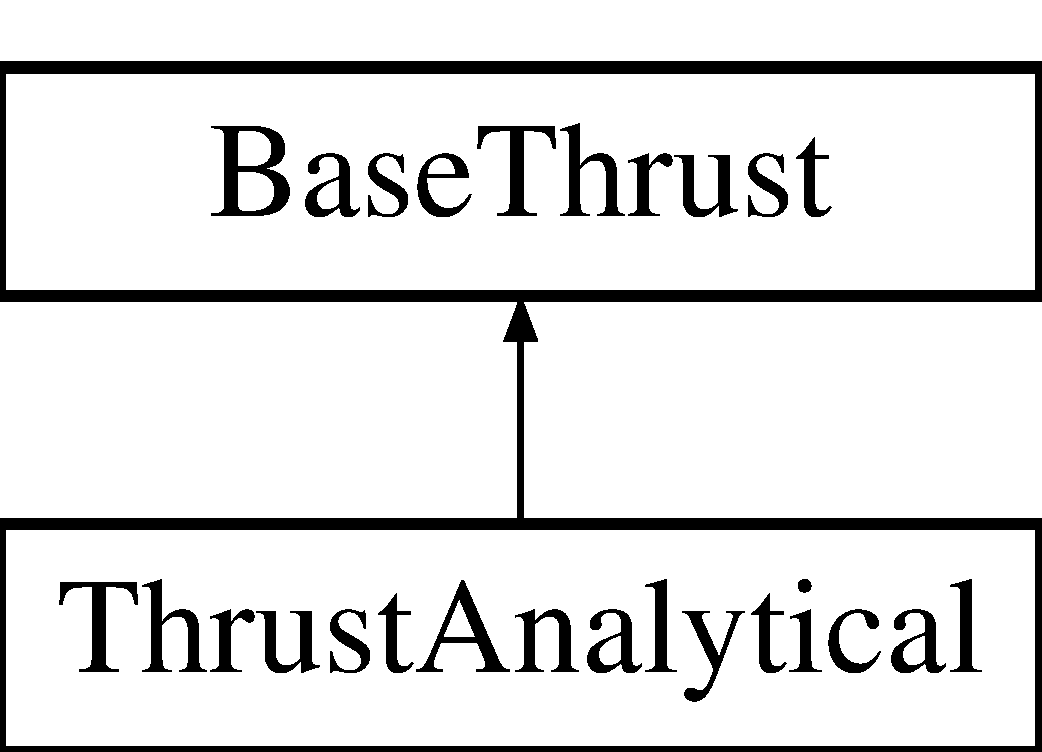
\includegraphics[height=2.000000cm]{group___engine}
\end{center}
\end{figure}
\subsubsection*{Public Member Functions}
\begin{DoxyCompactItemize}
\item 
\mbox{\Hypertarget{group___engine_a19885a6a70bfc4c02e2d8f310af9f22e}\label{group___engine_a19885a6a70bfc4c02e2d8f310af9f22e}} 
\hyperlink{group___engine_a19885a6a70bfc4c02e2d8f310af9f22e}{Base\+Thrust} ()
\begin{DoxyCompactList}\small\item\em constructor \end{DoxyCompactList}\item 
\mbox{\Hypertarget{group___engine_a554955351c2acfe7a46c00fe056c5c6c}\label{group___engine_a554955351c2acfe7a46c00fe056c5c6c}} 
\hyperlink{group___engine_a554955351c2acfe7a46c00fe056c5c6c}{$\sim$\+Base\+Thrust} ()
\begin{DoxyCompactList}\small\item\em destructor \end{DoxyCompactList}\item 
void \hyperlink{group___engine_a869359a1b2b7cddcbe5979d6a1cf5eac}{update\+Thrust} (Float64 Flight\+Time, Atmosphere\+Struct \&Atmo\+Data, Aerodynamic\+Struct \&Aero\+Data, Airframe\+Struct \&Airframe\+Data, Thrust\+Struct \&Thrust\+Data)
\item 
void \hyperlink{group___engine_a1a9a88e6c05cc0b2564522347365900c}{init\+Thrust} ()
\item 
virtual void \hyperlink{group___engine_ac578e683598739655ce52ea85d97362b}{calc\+Thrust} (Float64 Flight\+Time, Atmosphere\+Struct \&Atmo\+Data, Aerodynamic\+Struct \&Aero\+Data, Airframe\+Struct \&Airframe\+Data, Thrust\+Struct \&Thrust\+Data)
\begin{DoxyCompactList}\small\item\em calculate thrust forces and moments \end{DoxyCompactList}\item 
\mbox{\Hypertarget{group___engine_a373a66f6415f783f0e70782763ae45c7}\label{group___engine_a373a66f6415f783f0e70782763ae45c7}} 
virtual void {\bfseries initialize\+Thrust} ()
\end{DoxyCompactItemize}


\paragraph{Member Function Documentation}
\mbox{\Hypertarget{group___engine_ac578e683598739655ce52ea85d97362b}\label{group___engine_ac578e683598739655ce52ea85d97362b}} 
\index{Base\+Thrust@{Base\+Thrust}!calc\+Thrust@{calc\+Thrust}}
\index{calc\+Thrust@{calc\+Thrust}!Base\+Thrust@{Base\+Thrust}}
\subparagraph{\texorpdfstring{calc\+Thrust()}{calcThrust()}}
{\footnotesize\ttfamily void Base\+Thrust\+::calc\+Thrust (\begin{DoxyParamCaption}\item[{Float64}]{Flight\+Time,  }\item[{Atmosphere\+Struct \&}]{Atmo\+Data,  }\item[{Aerodynamic\+Struct \&}]{Aero\+Data,  }\item[{Airframe\+Struct \&}]{Airframe\+Data,  }\item[{Thrust\+Struct \&}]{Thrust\+Data }\end{DoxyParamCaption})\hspace{0.3cm}{\ttfamily [virtual]}}



calculate thrust forces and moments 


\begin{DoxyParams}{Parameters}
{\em Flight\+Time} & \\
\hline
{\em Atmo\+Data} & get current atmospheric data \\
\hline
{\em Aero\+Data} & get mach number \\
\hline
{\em Airframe\+Data} & get current throttle stick position \\
\hline
\end{DoxyParams}
\begin{DoxyReturn}{Returns}
current thrust data is stored in Thrust\+Struct 
\end{DoxyReturn}


Reimplemented in \hyperlink{group___engine_a521b775b57dc2324f09496efb8b12452}{Thrust\+Analytical}.



Definition at line \hyperlink{_base_thrust_8cpp_source_l00021}{21} of file \hyperlink{_base_thrust_8cpp_source}{Base\+Thrust.\+cpp}.

\mbox{\Hypertarget{group___engine_a1a9a88e6c05cc0b2564522347365900c}\label{group___engine_a1a9a88e6c05cc0b2564522347365900c}} 
\index{Base\+Thrust@{Base\+Thrust}!init\+Thrust@{init\+Thrust}}
\index{init\+Thrust@{init\+Thrust}!Base\+Thrust@{Base\+Thrust}}
\subparagraph{\texorpdfstring{init\+Thrust()}{initThrust()}}
{\footnotesize\ttfamily void Base\+Thrust\+::init\+Thrust (\begin{DoxyParamCaption}{ }\end{DoxyParamCaption})}

The init function from the selected engine is called by a pointer. 

Definition at line \hyperlink{_base_thrust_8cpp_source_l00011}{11} of file \hyperlink{_base_thrust_8cpp_source}{Base\+Thrust.\+cpp}.

\mbox{\Hypertarget{group___engine_a869359a1b2b7cddcbe5979d6a1cf5eac}\label{group___engine_a869359a1b2b7cddcbe5979d6a1cf5eac}} 
\index{Base\+Thrust@{Base\+Thrust}!update\+Thrust@{update\+Thrust}}
\index{update\+Thrust@{update\+Thrust}!Base\+Thrust@{Base\+Thrust}}
\subparagraph{\texorpdfstring{update\+Thrust()}{updateThrust()}}
{\footnotesize\ttfamily void Base\+Thrust\+::update\+Thrust (\begin{DoxyParamCaption}\item[{Float64}]{Flight\+Time,  }\item[{Atmosphere\+Struct \&}]{Atmo\+Data,  }\item[{Aerodynamic\+Struct \&}]{Aero\+Data,  }\item[{Airframe\+Struct \&}]{Airframe\+Data,  }\item[{Thrust\+Struct \&}]{Thrust\+Data }\end{DoxyParamCaption})}

The update function from the selected engine is called by a pointer. 

Definition at line \hyperlink{_base_thrust_8cpp_source_l00031}{31} of file \hyperlink{_base_thrust_8cpp_source}{Base\+Thrust.\+cpp}.

\index{Engine@{Engine}}\label{class_engine}
\Hypertarget{group___engine_class_engine}
\subsubsection{class Engine}


Definition at line \hyperlink{_engine_8h_source_l00015}{15} of file \hyperlink{_engine_8h_source}{Engine.\+h}.

\subsubsection*{Public Member Functions}
\begin{DoxyCompactItemize}
\item 
\mbox{\Hypertarget{group___engine_a8c98683b0a3aa28d8ab72a8bcd0d52f2}\label{group___engine_a8c98683b0a3aa28d8ab72a8bcd0d52f2}} 
\hyperlink{group___engine_a8c98683b0a3aa28d8ab72a8bcd0d52f2}{Engine} ()
\begin{DoxyCompactList}\small\item\em constructor \end{DoxyCompactList}\item 
\mbox{\Hypertarget{group___engine_a8ef7030a089ecb30bbfcb9e43094717a}\label{group___engine_a8ef7030a089ecb30bbfcb9e43094717a}} 
\hyperlink{group___engine_a8ef7030a089ecb30bbfcb9e43094717a}{$\sim$\+Engine} ()
\begin{DoxyCompactList}\small\item\em destructor \end{DoxyCompactList}\item 
void \hyperlink{group___engine_ac33371d6fff86c0c8e14495f10046d9a}{select\+Engine\+Type} (int type)
\begin{DoxyCompactList}\small\item\em select \hyperlink{group___engine_class_engine}{Engine} Type depending on input file \end{DoxyCompactList}\item 
\mbox{\Hypertarget{group___engine_aca6cc0dc7d537295123630a219142337}\label{group___engine_aca6cc0dc7d537295123630a219142337}} 
void \hyperlink{group___engine_aca6cc0dc7d537295123630a219142337}{init\+Engine} ()
\begin{DoxyCompactList}\small\item\em initilization of engine specific data \end{DoxyCompactList}\item 
void \hyperlink{group___engine_a9e16100ffd33cf8ec632257795c03865}{update\+Engine} (Float64 Flight\+Time, Atmosphere\+Struct \&Atmo\+Data, Aerodynamic\+Struct \&Aero\+Data, Airframe\+Struct \&Airframe\+Data, Thrust\+Struct \&Thrust\+Data)
\begin{DoxyCompactList}\small\item\em calculate thrust forces and moments \end{DoxyCompactList}\end{DoxyCompactItemize}


\paragraph{Member Function Documentation}
\mbox{\Hypertarget{group___engine_ac33371d6fff86c0c8e14495f10046d9a}\label{group___engine_ac33371d6fff86c0c8e14495f10046d9a}} 
\index{Engine@{Engine}!select\+Engine\+Type@{select\+Engine\+Type}}
\index{select\+Engine\+Type@{select\+Engine\+Type}!Engine@{Engine}}
\subparagraph{\texorpdfstring{select\+Engine\+Type()}{selectEngineType()}}
{\footnotesize\ttfamily void Engine\+::select\+Engine\+Type (\begin{DoxyParamCaption}\item[{int}]{type }\end{DoxyParamCaption})}



select \hyperlink{group___engine_class_engine}{Engine} Type depending on input file 


\begin{DoxyParams}{Parameters}
{\em type} & specific integer to select desired engine \\
\hline
\end{DoxyParams}


Definition at line \hyperlink{_engine_8cpp_source_l00015}{15} of file \hyperlink{_engine_8cpp_source}{Engine.\+cpp}.

\mbox{\Hypertarget{group___engine_a9e16100ffd33cf8ec632257795c03865}\label{group___engine_a9e16100ffd33cf8ec632257795c03865}} 
\index{Engine@{Engine}!update\+Engine@{update\+Engine}}
\index{update\+Engine@{update\+Engine}!Engine@{Engine}}
\subparagraph{\texorpdfstring{update\+Engine()}{updateEngine()}}
{\footnotesize\ttfamily void Engine\+::update\+Engine (\begin{DoxyParamCaption}\item[{Float64}]{Flight\+Time,  }\item[{Atmosphere\+Struct \&}]{Atmo\+Data,  }\item[{Aerodynamic\+Struct \&}]{Aero\+Data,  }\item[{Airframe\+Struct \&}]{Airframe\+Data,  }\item[{Thrust\+Struct \&}]{Thrust\+Data }\end{DoxyParamCaption})}



calculate thrust forces and moments 


\begin{DoxyParams}{Parameters}
{\em Flight\+Time} & \\
\hline
{\em Atmo\+Data} & get current atmospheric data \\
\hline
{\em Aero\+Data} & get mach number \\
\hline
{\em Airframe\+Data} & get current throttle stick position \\
\hline
\end{DoxyParams}
\begin{DoxyReturn}{Returns}
current thrust data is stored in Thrust\+Struct 
\end{DoxyReturn}


Definition at line \hyperlink{_engine_8cpp_source_l00034}{34} of file \hyperlink{_engine_8cpp_source}{Engine.\+cpp}.

\index{Thrust\+Analytical@{Thrust\+Analytical}}\label{class_thrust_analytical}
\Hypertarget{group___engine_class_thrust_analytical}
\subsubsection{class Thrust\+Analytical}
\begin{DoxyAuthor}{Author}
Jan Olucak 
\end{DoxyAuthor}
\begin{DoxyDate}{Date}
25.\+11.\+2017 
\end{DoxyDate}
\begin{DoxyVersion}{Version}
1.\+0
\end{DoxyVersion}
Base Thrust class is the superclass for all engine models. Using pointer to base init and update function allows the user to extend the engine module with new engine models. 

Definition at line \hyperlink{_thrust_analytical_8h_source_l00020}{20} of file \hyperlink{_thrust_analytical_8h_source}{Thrust\+Analytical.\+h}.

Inheritance diagram for Thrust\+Analytical\+:\begin{figure}[H]
\begin{center}
\leavevmode
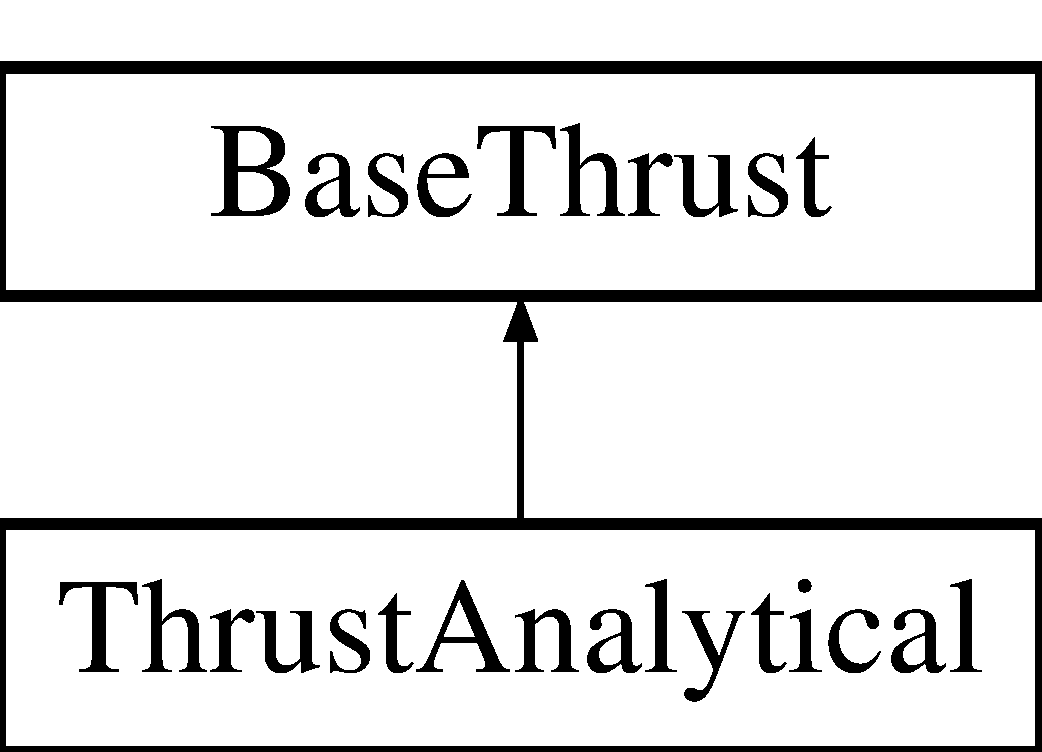
\includegraphics[height=2.000000cm]{group___engine}
\end{center}
\end{figure}
\subsubsection*{Public Member Functions}
\begin{DoxyCompactItemize}
\item 
\mbox{\Hypertarget{group___engine_a5c75949a22871e861090560adb2d5f18}\label{group___engine_a5c75949a22871e861090560adb2d5f18}} 
\hyperlink{group___engine_a5c75949a22871e861090560adb2d5f18}{Thrust\+Analytical} ()
\begin{DoxyCompactList}\small\item\em constructor \end{DoxyCompactList}\item 
\hyperlink{group___engine_aeaf9dd69c10812c673d6cfae0d7ca4fd}{$\sim$\+Thrust\+Analytical} ()
\begin{DoxyCompactList}\small\item\em destructor \end{DoxyCompactList}\item 
void \hyperlink{group___engine_a5c1db29b00aa92e9f22806b0ea482e05}{initialize\+Thrust} ()
\begin{DoxyCompactList}\small\item\em read in Data from Engine.\+dat \end{DoxyCompactList}\item 
void \hyperlink{group___engine_a521b775b57dc2324f09496efb8b12452}{calc\+Thrust} (Float64 Flight\+Time, Atmosphere\+Struct \&Atmo\+Data, Aerodynamic\+Struct \&Aero\+Data, Airframe\+Struct \&Airframe\+Data, Thrust\+Struct \&Thrust\+Data)
\begin{DoxyCompactList}\small\item\em calculate thrust forces and moments \end{DoxyCompactList}\end{DoxyCompactItemize}


\paragraph{Constructor \& Destructor Documentation}
\mbox{\Hypertarget{group___engine_aeaf9dd69c10812c673d6cfae0d7ca4fd}\label{group___engine_aeaf9dd69c10812c673d6cfae0d7ca4fd}} 
\index{Thrust\+Analytical@{Thrust\+Analytical}!````~Thrust\+Analytical@{$\sim$\+Thrust\+Analytical}}
\index{````~Thrust\+Analytical@{$\sim$\+Thrust\+Analytical}!Thrust\+Analytical@{Thrust\+Analytical}}
\subparagraph{\texorpdfstring{$\sim$\+Thrust\+Analytical()}{~ThrustAnalytical()}}
{\footnotesize\ttfamily Thrust\+Analytical\+::$\sim$\+Thrust\+Analytical (\begin{DoxyParamCaption}{ }\end{DoxyParamCaption})}



destructor 

destrcutor 

Definition at line \hyperlink{_thrust_analytical_8cpp_source_l00010}{10} of file \hyperlink{_thrust_analytical_8cpp_source}{Thrust\+Analytical.\+cpp}.



\paragraph{Member Function Documentation}
\mbox{\Hypertarget{group___engine_a521b775b57dc2324f09496efb8b12452}\label{group___engine_a521b775b57dc2324f09496efb8b12452}} 
\index{Thrust\+Analytical@{Thrust\+Analytical}!calc\+Thrust@{calc\+Thrust}}
\index{calc\+Thrust@{calc\+Thrust}!Thrust\+Analytical@{Thrust\+Analytical}}
\subparagraph{\texorpdfstring{calc\+Thrust()}{calcThrust()}}
{\footnotesize\ttfamily void Thrust\+Analytical\+::calc\+Thrust (\begin{DoxyParamCaption}\item[{Float64}]{Flight\+Time,  }\item[{Atmosphere\+Struct \&}]{Atmo\+Data,  }\item[{Aerodynamic\+Struct \&}]{Aero\+Data,  }\item[{Airframe\+Struct \&}]{Airframe\+Data,  }\item[{Thrust\+Struct \&}]{Thrust\+Data }\end{DoxyParamCaption})\hspace{0.3cm}{\ttfamily [virtual]}}



calculate thrust forces and moments 

calculation of thrust forces and moments


\begin{DoxyParams}{Parameters}
{\em Flight\+Time} & \\
\hline
{\em Atmo\+Data} & get current atmospheric data \\
\hline
{\em Aero\+Data} & get mach number \\
\hline
{\em Airframe\+Data} & get current throttle stick position \\
\hline
\end{DoxyParams}
\begin{DoxyReturn}{Returns}
current thrust data is stored in Thrust\+Struct 
\end{DoxyReturn}


Reimplemented from \hyperlink{group___engine_ac578e683598739655ce52ea85d97362b}{Base\+Thrust}.



Definition at line \hyperlink{_thrust_analytical_8cpp_source_l00030}{30} of file \hyperlink{_thrust_analytical_8cpp_source}{Thrust\+Analytical.\+cpp}.

\mbox{\Hypertarget{group___engine_a5c1db29b00aa92e9f22806b0ea482e05}\label{group___engine_a5c1db29b00aa92e9f22806b0ea482e05}} 
\index{Thrust\+Analytical@{Thrust\+Analytical}!initialize\+Thrust@{initialize\+Thrust}}
\index{initialize\+Thrust@{initialize\+Thrust}!Thrust\+Analytical@{Thrust\+Analytical}}
\subparagraph{\texorpdfstring{initialize\+Thrust()}{initializeThrust()}}
{\footnotesize\ttfamily void Thrust\+Analytical\+::initialize\+Thrust (\begin{DoxyParamCaption}{ }\end{DoxyParamCaption})\hspace{0.3cm}{\ttfamily [virtual]}}



read in Data from Engine.\+dat 

data is read in from Engine.\+dat and stored in private variables 

Reimplemented from \hyperlink{group___engine}{Base\+Thrust}.



Definition at line \hyperlink{_thrust_analytical_8cpp_source_l00015}{15} of file \hyperlink{_thrust_analytical_8cpp_source}{Thrust\+Analytical.\+cpp}.


\hypertarget{group___executive}{}\section{Executive}
\label{group___executive}\index{Executive@{Executive}}
\subsection*{Macros}
\begin{DoxyCompactItemize}
\item 
\#define \hyperlink{group___executive_ga9c58512ec990b4a3bb660c7f1f565373}{E\+X\+E\+C\+U\+T\+I\+V\+E\+\_\+\+\_\+H}
\end{DoxyCompactItemize}
\subsection*{Functions}
\begin{DoxyCompactItemize}
\item 
int \hyperlink{group___executive_gac4c0f8a8146b128f1b8f920e3a9c3b1e}{main} (int argv, char $\ast$argc\mbox{[}$\,$\mbox{]})
\end{DoxyCompactItemize}


\subsection{Detailed Description}
\begin{DoxyAuthor}{Author}
Jan Olucak 
\end{DoxyAuthor}
\begin{DoxyDate}{Date}
10.\+05.\+2018 
\end{DoxyDate}
\begin{DoxyVersion}{Version}
1.\+0
\end{DoxyVersion}
This file executes the actual simulation. The prefered models are read in. \hyperlink{class_aircraft}{Aircraft} class is initalized. The \hyperlink{class_trajectory}{Trajectory} is calculated 

\subsection{Macro Definition Documentation}
\mbox{\Hypertarget{group___executive_ga9c58512ec990b4a3bb660c7f1f565373}\label{group___executive_ga9c58512ec990b4a3bb660c7f1f565373}} 
\index{Executive@{Executive}!E\+X\+E\+C\+U\+T\+I\+V\+E\+\_\+\+\_\+H@{E\+X\+E\+C\+U\+T\+I\+V\+E\+\_\+\+\_\+H}}
\index{E\+X\+E\+C\+U\+T\+I\+V\+E\+\_\+\+\_\+H@{E\+X\+E\+C\+U\+T\+I\+V\+E\+\_\+\+\_\+H}!Executive@{Executive}}
\subsubsection{\texorpdfstring{E\+X\+E\+C\+U\+T\+I\+V\+E\+\_\+\+\_\+H}{EXECUTIVE\_\_H}}
{\footnotesize\ttfamily \#define E\+X\+E\+C\+U\+T\+I\+V\+E\+\_\+\+\_\+H}



Definition at line 11 of file Executive.\+cpp.



\subsection{Function Documentation}
\mbox{\Hypertarget{group___executive_gac4c0f8a8146b128f1b8f920e3a9c3b1e}\label{group___executive_gac4c0f8a8146b128f1b8f920e3a9c3b1e}} 
\index{Executive@{Executive}!main@{main}}
\index{main@{main}!Executive@{Executive}}
\subsubsection{\texorpdfstring{main()}{main()}}
{\footnotesize\ttfamily int main (\begin{DoxyParamCaption}\item[{int}]{argv,  }\item[{char $\ast$}]{argc\mbox{[}$\,$\mbox{]} }\end{DoxyParamCaption})}



Definition at line 28 of file Executive.\+cpp.


\hypertarget{group___g_p_s}{}\section{G\+PS}
\label{group___g_p_s}\index{G\+PS@{G\+PS}}
\subsection*{Classes}
\begin{DoxyCompactItemize}
\item 
class \hyperlink{class_base_g_p_s}{Base\+G\+PS}
\item 
class \hyperlink{classflawless_g_p_s}{flawless\+G\+PS}
\item 
class \hyperlink{class_g_p_s}{G\+PS}
\end{DoxyCompactItemize}


\subsection{Detailed Description}
\begin{DoxyAuthor}{Author}
Jan Olucak 
\end{DoxyAuthor}
\begin{DoxyDate}{Date}
02.\+01.\+2018 
\end{DoxyDate}
\begin{DoxyVersion}{Version}
1.\+0
\end{DoxyVersion}
\hyperlink{class_g_p_s}{G\+PS} class is used to call the desired \hyperlink{class_g_p_s}{G\+PS} model. The \hyperlink{class_g_p_s}{G\+PS} model is selected from General.\+dat input file. 
\hypertarget{group___guidance}{}\section{Guidance}
\label{group___guidance}\index{Guidance@{Guidance}}
\subsection*{Classes}
\begin{DoxyCompactItemize}
\item 
class \hyperlink{classacc_table}{acc\+Table}
\item 
class \hyperlink{class_base_guidance}{Base\+Guidance}
\item 
class \hyperlink{class_guidance}{Guidance}
\end{DoxyCompactItemize}


\subsection{Detailed Description}
\begin{DoxyAuthor}{Author}
Jan Olucak 
\end{DoxyAuthor}
\begin{DoxyDate}{Date}
23.\+12.\+2017 
\end{DoxyDate}
\begin{DoxyVersion}{Version}
1.\+0
\end{DoxyVersion}
\hyperlink{class_guidance}{Guidance} class is used to call the desired \hyperlink{class_guidance}{Guidance} model. 
\hypertarget{group___i_m_u}{}\section{I\+MU}
\label{group___i_m_u}\index{I\+MU@{I\+MU}}
\subsection*{Classes}
\begin{DoxyCompactItemize}
\item 
class \hyperlink{class_base_i_m_u}{Base\+I\+MU}
\item 
class \hyperlink{classflawless_i_m_u}{flawless\+I\+MU}
\item 
class \hyperlink{class_i_m_u}{I\+MU}
\end{DoxyCompactItemize}


\subsection{Detailed Description}
\begin{DoxyAuthor}{Author}
Jan Olucak 
\end{DoxyAuthor}
\begin{DoxyDate}{Date}
02.\+01.\+2018 
\end{DoxyDate}
\begin{DoxyVersion}{Version}
1.\+0
\end{DoxyVersion}
\hyperlink{class_i_m_u}{I\+MU} class is used to call the desired \hyperlink{class_i_m_u}{I\+MU} model. The \hyperlink{class_i_m_u}{I\+MU} model is selected from General.\+dat input file. 
\hypertarget{group___moduletest}{}\section{Moduletest}
\label{group___moduletest}\index{Moduletest@{Moduletest}}
\subsection*{Functions}
\begin{DoxyCompactItemize}
\item 
void \hyperlink{group___moduletest_gad43a0024f4d65199da1e138730b77366}{Atmosphere\+Test} ()
\begin{DoxyCompactList}\small\item\em The atmospheric model is tested. Hence altitude is increased up to 10000m. Atmospheric data is stored and plotted in Matlab. The plots are compared to characteritic trends. \end{DoxyCompactList}\item 
void \hyperlink{group___moduletest_gaa6c5f38a2905aa430098c2bbc54294ae}{Aerodynamic\+Test} (Sim\+D\+Preference \&Sim\+Pref)
\begin{DoxyCompactList}\small\item\em Datcom aerodynamic is tested. Therefor a windtunnel is simulate. Within loops Angle of attack, elevator angle and mach are varied. Characterisitcs (e.\+g. drag polar) are calculated for several flight states. Only longitudinal aerodynamic is tested. \end{DoxyCompactList}\item 
void \hyperlink{group___moduletest_ga506ca9f8cae8f5ef59e2ae58b867384e}{Guidance\+Test} (Sim\+D\+Preference \&Sim\+Pref)
\item 
void \hyperlink{group___moduletest_ga3f0bd743f32651aeae72d8d92cd97104}{Trajectory\+Test} (Sim\+D\+Preference \&Sim\+Pref)
\item 
int \hyperlink{group___moduletest_gae66f6b31b5ad750f1fe042a706a4e3d4}{main} ()
\end{DoxyCompactItemize}


\subsection{Detailed Description}
\begin{DoxyAuthor}{Author}
Jan Olucak 
\end{DoxyAuthor}
\begin{DoxyDate}{Date}
25.\+11.\+2017 
\end{DoxyDate}
\begin{DoxyVersion}{Version}
1.\+0
\end{DoxyVersion}
\hyperlink{_module_test_8cpp}{Module\+Test.\+cpp} cotains module tests for several modules. Some modules need a complete simulation to be tested 

\subsection{Function Documentation}
\mbox{\Hypertarget{group___moduletest_gaa6c5f38a2905aa430098c2bbc54294ae}\label{group___moduletest_gaa6c5f38a2905aa430098c2bbc54294ae}} 
\index{Moduletest@{Moduletest}!Aerodynamic\+Test@{Aerodynamic\+Test}}
\index{Aerodynamic\+Test@{Aerodynamic\+Test}!Moduletest@{Moduletest}}
\subsubsection{\texorpdfstring{Aerodynamic\+Test()}{AerodynamicTest()}}
{\footnotesize\ttfamily void Aerodynamic\+Test (\begin{DoxyParamCaption}\item[{Sim\+D\+Preference \&}]{Sim\+Pref }\end{DoxyParamCaption})}



Datcom aerodynamic is tested. Therefor a windtunnel is simulate. Within loops Angle of attack, elevator angle and mach are varied. Characterisitcs (e.\+g. drag polar) are calculated for several flight states. Only longitudinal aerodynamic is tested. 

1) Initialization of models and data

2) aircraft characterisitcs and simulation data are read in

3) Definition of Output

4) 3 loops simulate a wind tunnel with varying flight states 

Definition at line 73 of file Module\+Test.\+cpp.



Referenced by main().

\mbox{\Hypertarget{group___moduletest_gad43a0024f4d65199da1e138730b77366}\label{group___moduletest_gad43a0024f4d65199da1e138730b77366}} 
\index{Moduletest@{Moduletest}!Atmosphere\+Test@{Atmosphere\+Test}}
\index{Atmosphere\+Test@{Atmosphere\+Test}!Moduletest@{Moduletest}}
\subsubsection{\texorpdfstring{Atmosphere\+Test()}{AtmosphereTest()}}
{\footnotesize\ttfamily void Atmosphere\+Test (\begin{DoxyParamCaption}{ }\end{DoxyParamCaption})}



The atmospheric model is tested. Hence altitude is increased up to 10000m. Atmospheric data is stored and plotted in Matlab. The plots are compared to characteritic trends. 

1) Initialization of models and data

2) Loop increases altitude; data is stored to outputfile 

Definition at line 38 of file Module\+Test.\+cpp.



Referenced by main().

\mbox{\Hypertarget{group___moduletest_ga506ca9f8cae8f5ef59e2ae58b867384e}\label{group___moduletest_ga506ca9f8cae8f5ef59e2ae58b867384e}} 
\index{Moduletest@{Moduletest}!Guidance\+Test@{Guidance\+Test}}
\index{Guidance\+Test@{Guidance\+Test}!Moduletest@{Moduletest}}
\subsubsection{\texorpdfstring{Guidance\+Test()}{GuidanceTest()}}
{\footnotesize\ttfamily void Guidance\+Test (\begin{DoxyParamCaption}\item[{Sim\+D\+Preference \&}]{Sim\+Pref }\end{DoxyParamCaption})}



Definition at line 196 of file Module\+Test.\+cpp.



Referenced by main().

\mbox{\Hypertarget{group___moduletest_gae66f6b31b5ad750f1fe042a706a4e3d4}\label{group___moduletest_gae66f6b31b5ad750f1fe042a706a4e3d4}} 
\index{Moduletest@{Moduletest}!main@{main}}
\index{main@{main}!Moduletest@{Moduletest}}
\subsubsection{\texorpdfstring{main()}{main()}}
{\footnotesize\ttfamily int main (\begin{DoxyParamCaption}{ }\end{DoxyParamCaption})}



Definition at line 373 of file Module\+Test.\+cpp.

\mbox{\Hypertarget{group___moduletest_ga3f0bd743f32651aeae72d8d92cd97104}\label{group___moduletest_ga3f0bd743f32651aeae72d8d92cd97104}} 
\index{Moduletest@{Moduletest}!Trajectory\+Test@{Trajectory\+Test}}
\index{Trajectory\+Test@{Trajectory\+Test}!Moduletest@{Moduletest}}
\subsubsection{\texorpdfstring{Trajectory\+Test()}{TrajectoryTest()}}
{\footnotesize\ttfamily void Trajectory\+Test (\begin{DoxyParamCaption}\item[{Sim\+D\+Preference \&}]{Sim\+Pref }\end{DoxyParamCaption})}



Definition at line 276 of file Module\+Test.\+cpp.


\hypertarget{group___navigtion}{}\section{Navigation}
\label{group___navigtion}\index{Navigation@{Navigation}}
\subsection*{Classes}
\begin{DoxyCompactItemize}
\item 
class \hyperlink{class_navigation}{Navigation}
\end{DoxyCompactItemize}


\subsection{Detailed Description}
\begin{DoxyAuthor}{Author}
Jan Olucak 
\end{DoxyAuthor}
\begin{DoxyDate}{Date}
02.\+01.\+2018 
\end{DoxyDate}
\begin{DoxyVersion}{Version}
1.\+0
\end{DoxyVersion}
\hyperlink{class_navigation}{Navigation} class is used to call the desired navigation model. The navigation model is selected from General.\+dat input file. 
\hypertarget{group___tools}{}\section{Tools}
\label{group___tools}\index{Tools@{Tools}}
\subsection*{Classes}
\begin{DoxyCompactItemize}
\item 
class \hyperlink{class_data_logger}{Data\+Logger}
\item 
class \hyperlink{class_mat_file_reader}{Mat\+File\+Reader}
\item 
class \hyperlink{class_transformation}{Transformation}
\end{DoxyCompactItemize}
\begin{DoxyCompactItemize}
\item 
const \hyperlink{group___tools_ga3f1431cb9f76da10f59246d1d743dc2c}{Float64} \hyperlink{group___tools_ga6e7b8e4a71fb3f6d37718ac5d614f560}{G\+A\+M\+MA} = 1.\+4
\item 
const \hyperlink{group___tools_ga3f1431cb9f76da10f59246d1d743dc2c}{Float64} \hyperlink{group___tools_ga50141cecfc14099c41bee22b4f166637}{G\+A\+S\+\_\+\+C\+O\+N\+S\+T\+A\+NT} = 287
\item 
const \hyperlink{group___tools_ga3f1431cb9f76da10f59246d1d743dc2c}{Float64} \hyperlink{group___tools_ga4350dd604b08011751eaca3d76213582}{R\+H\+O\+\_\+0} = 1.\+225
\item 
const \hyperlink{group___tools_ga3f1431cb9f76da10f59246d1d743dc2c}{Float64} \hyperlink{group___tools_gac3a28ac509d7e1dff951cc777889cc93}{PI} = 3.\+1416
\item 
const \hyperlink{group___tools_ga3f1431cb9f76da10f59246d1d743dc2c}{Float64} \hyperlink{group___tools_gad0d838a1206faf55a621d5ec8f1e896d}{G\+R\+A\+V\+I\+T\+A\+T\+I\+O\+N\+A\+L\+\_\+\+C\+O\+N\+S\+T\+A\+NT} = 9.\+80665
\end{DoxyCompactItemize}
\begin{DoxyCompactItemize}
\item 
typedef double \hyperlink{group___tools_ga3f1431cb9f76da10f59246d1d743dc2c}{Float64}
\item 
typedef float \hyperlink{group___tools_ga87d38f886e617ced2698fc55afa07637}{Float32}
\end{DoxyCompactItemize}
\begin{DoxyCompactItemize}
\item 
typedef double \hyperlink{group___tools_ga3f1431cb9f76da10f59246d1d743dc2c}{Float64}
\item 
{\footnotesize template$<$typename T $>$ }\\T \hyperlink{group___tools_ga33942ddaef2c066dde4aac1457e7ed9d}{Euler\+Integration} (T v1, T v2, \hyperlink{group___tools_ga3f1431cb9f76da10f59246d1d743dc2c}{Float64} dt)
\end{DoxyCompactItemize}


\subsection{Detailed Description}
\begin{DoxyAuthor}{Author}
Jan Olucak 
\end{DoxyAuthor}
\begin{DoxyDate}{Date}
25.\+11.\+2017 
\end{DoxyDate}
\begin{DoxyVersion}{Version}
1.\+0
\end{DoxyVersion}
Data Logger is a class to write simulation data to an outputfile. 

\subsection{Typedef Documentation}
\mbox{\Hypertarget{group___tools_ga87d38f886e617ced2698fc55afa07637}\label{group___tools_ga87d38f886e617ced2698fc55afa07637}} 
\index{Tools@{Tools}!Float32@{Float32}}
\index{Float32@{Float32}!Tools@{Tools}}
\subsubsection{\texorpdfstring{Float32}{Float32}}
{\footnotesize\ttfamily typedef float \hyperlink{group___tools_ga87d38f886e617ced2698fc55afa07637}{Float32}}



Definition at line 14 of file Independet\+Data\+Types.\+h.

\mbox{\Hypertarget{group___tools_ga3f1431cb9f76da10f59246d1d743dc2c}\label{group___tools_ga3f1431cb9f76da10f59246d1d743dc2c}} 
\index{Tools@{Tools}!Float64@{Float64}}
\index{Float64@{Float64}!Tools@{Tools}}
\subsubsection{\texorpdfstring{Float64}{Float64}\hspace{0.1cm}{\footnotesize\ttfamily [1/2]}}
{\footnotesize\ttfamily typedef double \hyperlink{group___tools_ga3f1431cb9f76da10f59246d1d743dc2c}{Float64}}

\begin{DoxyAuthor}{Author}
Jan Olucak 
\end{DoxyAuthor}
\begin{DoxyDate}{Date}
25.\+11.\+2017 
\end{DoxyDate}
\begin{DoxyVersion}{Version}
1.\+0
\end{DoxyVersion}
O\+D\+E\+Solver provide methods for numerical integration 

Definition at line 10 of file O\+D\+E\+Solver.\+cpp.

\mbox{\Hypertarget{group___tools_ga3f1431cb9f76da10f59246d1d743dc2c}\label{group___tools_ga3f1431cb9f76da10f59246d1d743dc2c}} 
\index{Tools@{Tools}!Float64@{Float64}}
\index{Float64@{Float64}!Tools@{Tools}}
\subsubsection{\texorpdfstring{Float64}{Float64}\hspace{0.1cm}{\footnotesize\ttfamily [2/2]}}
{\footnotesize\ttfamily typedef double \hyperlink{group___tools_ga3f1431cb9f76da10f59246d1d743dc2c}{Float64}}

\begin{DoxyAuthor}{Author}
Jan Olucak 
\end{DoxyAuthor}
\begin{DoxyDate}{Date}
25.\+11.\+2017 
\end{DoxyDate}
\begin{DoxyVersion}{Version}
1.\+0
\end{DoxyVersion}
Provides independet data types 

Definition at line 13 of file Independet\+Data\+Types.\+h.



\subsection{Function Documentation}
\mbox{\Hypertarget{group___tools_ga33942ddaef2c066dde4aac1457e7ed9d}\label{group___tools_ga33942ddaef2c066dde4aac1457e7ed9d}} 
\index{Tools@{Tools}!Euler\+Integration@{Euler\+Integration}}
\index{Euler\+Integration@{Euler\+Integration}!Tools@{Tools}}
\subsubsection{\texorpdfstring{Euler\+Integration()}{EulerIntegration()}}
{\footnotesize\ttfamily template$<$typename T $>$ \\
T Euler\+Integration (\begin{DoxyParamCaption}\item[{T}]{v1,  }\item[{T}]{v2,  }\item[{\hyperlink{group___tools_ga3f1431cb9f76da10f59246d1d743dc2c}{Float64}}]{dt }\end{DoxyParamCaption})}



Definition at line 13 of file O\+D\+E\+Solver.\+cpp.



Referenced by Trajectory6\+Dof\+::integration\+Trajectory(), Unit\+Test1\+::\+T\+E\+S\+T\+\_\+\+C\+L\+A\+S\+S(), flawless\+I\+M\+U\+::update\+I\+M\+U(), and flawless\+Navigation\+::update\+Navigation().



\subsection{Variable Documentation}
\mbox{\Hypertarget{group___tools_ga6e7b8e4a71fb3f6d37718ac5d614f560}\label{group___tools_ga6e7b8e4a71fb3f6d37718ac5d614f560}} 
\index{Tools@{Tools}!G\+A\+M\+MA@{G\+A\+M\+MA}}
\index{G\+A\+M\+MA@{G\+A\+M\+MA}!Tools@{Tools}}
\subsubsection{\texorpdfstring{G\+A\+M\+MA}{GAMMA}}
{\footnotesize\ttfamily const \hyperlink{group___tools_ga3f1431cb9f76da10f59246d1d743dc2c}{Float64} G\+A\+M\+MA = 1.\+4}

\begin{DoxyAuthor}{Author}
Jan Olucak 
\end{DoxyAuthor}
\begin{DoxyDate}{Date}
25.\+11.\+2017 
\end{DoxyDate}
\begin{DoxyVersion}{Version}
1.\+0
\end{DoxyVersion}
Provides physical and mathematical constants 

Definition at line 15 of file Constants.\+h.



Referenced by Atmopshere\+::update\+Atmosphere().

\mbox{\Hypertarget{group___tools_ga50141cecfc14099c41bee22b4f166637}\label{group___tools_ga50141cecfc14099c41bee22b4f166637}} 
\index{Tools@{Tools}!G\+A\+S\+\_\+\+C\+O\+N\+S\+T\+A\+NT@{G\+A\+S\+\_\+\+C\+O\+N\+S\+T\+A\+NT}}
\index{G\+A\+S\+\_\+\+C\+O\+N\+S\+T\+A\+NT@{G\+A\+S\+\_\+\+C\+O\+N\+S\+T\+A\+NT}!Tools@{Tools}}
\subsubsection{\texorpdfstring{G\+A\+S\+\_\+\+C\+O\+N\+S\+T\+A\+NT}{GAS\_CONSTANT}}
{\footnotesize\ttfamily const \hyperlink{group___tools_ga3f1431cb9f76da10f59246d1d743dc2c}{Float64} G\+A\+S\+\_\+\+C\+O\+N\+S\+T\+A\+NT = 287}



Definition at line 16 of file Constants.\+h.



Referenced by Atmopshere\+::update\+Atmosphere().

\mbox{\Hypertarget{group___tools_gad0d838a1206faf55a621d5ec8f1e896d}\label{group___tools_gad0d838a1206faf55a621d5ec8f1e896d}} 
\index{Tools@{Tools}!G\+R\+A\+V\+I\+T\+A\+T\+I\+O\+N\+A\+L\+\_\+\+C\+O\+N\+S\+T\+A\+NT@{G\+R\+A\+V\+I\+T\+A\+T\+I\+O\+N\+A\+L\+\_\+\+C\+O\+N\+S\+T\+A\+NT}}
\index{G\+R\+A\+V\+I\+T\+A\+T\+I\+O\+N\+A\+L\+\_\+\+C\+O\+N\+S\+T\+A\+NT@{G\+R\+A\+V\+I\+T\+A\+T\+I\+O\+N\+A\+L\+\_\+\+C\+O\+N\+S\+T\+A\+NT}!Tools@{Tools}}
\subsubsection{\texorpdfstring{G\+R\+A\+V\+I\+T\+A\+T\+I\+O\+N\+A\+L\+\_\+\+C\+O\+N\+S\+T\+A\+NT}{GRAVITATIONAL\_CONSTANT}}
{\footnotesize\ttfamily const \hyperlink{group___tools_ga3f1431cb9f76da10f59246d1d743dc2c}{Float64} G\+R\+A\+V\+I\+T\+A\+T\+I\+O\+N\+A\+L\+\_\+\+C\+O\+N\+S\+T\+A\+NT = 9.\+80665}



Definition at line 19 of file Constants.\+h.



Referenced by acc\+Table\+::update\+Guidance(), and Airframe\+::update\+Translational().

\mbox{\Hypertarget{group___tools_gac3a28ac509d7e1dff951cc777889cc93}\label{group___tools_gac3a28ac509d7e1dff951cc777889cc93}} 
\index{Tools@{Tools}!PI@{PI}}
\index{PI@{PI}!Tools@{Tools}}
\subsubsection{\texorpdfstring{PI}{PI}}
{\footnotesize\ttfamily const \hyperlink{group___tools_ga3f1431cb9f76da10f59246d1d743dc2c}{Float64} PI = 3.\+1416}



Definition at line 18 of file Constants.\+h.



Referenced by Aerodynamic\+Test(), D\+A\+T\+C\+O\+M\+Aerodymamic\+::update\+Aerodynamic(), State\+Controller\+::update\+State\+Controller(), and Airframe\+::update\+Translational().

\mbox{\Hypertarget{group___tools_ga4350dd604b08011751eaca3d76213582}\label{group___tools_ga4350dd604b08011751eaca3d76213582}} 
\index{Tools@{Tools}!R\+H\+O\+\_\+0@{R\+H\+O\+\_\+0}}
\index{R\+H\+O\+\_\+0@{R\+H\+O\+\_\+0}!Tools@{Tools}}
\subsubsection{\texorpdfstring{R\+H\+O\+\_\+0}{RHO\_0}}
{\footnotesize\ttfamily const \hyperlink{group___tools_ga3f1431cb9f76da10f59246d1d743dc2c}{Float64} R\+H\+O\+\_\+0 = 1.\+225}



Definition at line 17 of file Constants.\+h.



Referenced by Thrust\+Analytical\+::update\+Thrust().


\hypertarget{group___trajectory}{}\section{Trajectory}
\label{group___trajectory}\index{Trajectory@{Trajectory}}
\subsection*{Classes}
\begin{DoxyCompactItemize}
\item 
class \hyperlink{group___trajectory_class_base_trajectory}{Base\+Trajectory}
\item 
class \hyperlink{group___trajectory_class_trajectory}{Trajectory}
\item 
class \hyperlink{group___trajectory_class_trajectory3_dof}{Trajectory3\+Dof}
\item 
class \hyperlink{group___trajectory_class_trajectory6_dof}{Trajectory6\+Dof}
\end{DoxyCompactItemize}
\subsection*{Functions}
\begin{DoxyCompactItemize}
\item 
\mbox{\Hypertarget{group___trajectory_ga8d2001c718f24b178ca0dd84ec1a3960}\label{group___trajectory_ga8d2001c718f24b178ca0dd84ec1a3960}} 
{\bfseries Trajectory\+::\+Trajectory} (Sim\+D\+Preference \&Sim\+Pref)
\item 
\mbox{\Hypertarget{group___trajectory_gade7c1162e2dbb9b6a58e4b14edc47a23}\label{group___trajectory_gade7c1162e2dbb9b6a58e4b14edc47a23}} 
void {\bfseries Trajectory\+::select\+Trajectory} (int type)
\item 
\mbox{\Hypertarget{group___trajectory_ga281eabbd48c553f15f393ed906642a3f}\label{group___trajectory_ga281eabbd48c553f15f393ed906642a3f}} 
void {\bfseries Trajectory\+::update\+Trajectory} (\hyperlink{group___tools_ga3f1431cb9f76da10f59246d1d743dc2c}{Float64} Flight\+Time, Atmosphere\+Struct \&Atmo\+Data, Aerodynamic\+Struct \&Aero\+Data, Airframe\+Struct \&Airframe\+Data, Thrust\+Struct \&Thrust\+Data, Guidance\+Struct \&Guidance\+Data)
\item 
\mbox{\Hypertarget{group___trajectory_ga3104447fe2b96a3471362eec02e937f0}\label{group___trajectory_ga3104447fe2b96a3471362eec02e937f0}} 
void {\bfseries Trajectory\+::init\+Trajectory} (Aerodynamic\+Struct \&Aero\+Data, Airframe\+Struct \&Airframe\+Data, Thrust\+Struct \&Thrust\+Data, Aircraft\+Struct \&Aircraft\+Data, Guidance\+Struct \&Guidance\+Data)
\item 
\mbox{\Hypertarget{group___trajectory_ga304011b4296d0ac38bcee32a760405ea}\label{group___trajectory_ga304011b4296d0ac38bcee32a760405ea}} 
virtual void {\bfseries Trajectory3\+Dof\+::init\+Trajectory} (Aerodynamic\+Struct \&Aero\+Data, Airframe\+Struct \&Airframe\+Data, Thrust\+Struct \&Thrust\+Data, Aircraft\+Struct \&Aircraft\+Data, Guidance\+Struct \&Guidance\+Data)
\item 
\mbox{\Hypertarget{group___trajectory_gafc82799754ef6c2813bc862c5bc1c3e9}\label{group___trajectory_gafc82799754ef6c2813bc862c5bc1c3e9}} 
virtual void {\bfseries Trajectory3\+Dof\+::update\+Trajectory} (\hyperlink{group___tools_ga3f1431cb9f76da10f59246d1d743dc2c}{Float64} Flight\+Time, Atmosphere\+Struct \&Atmo\+Data, Aerodynamic\+Struct \&Aero\+Data, Airframe\+Struct \&Airframe\+Data, Thrust\+Struct \&Thrust\+Data, Guidance\+Struct \&Guidance\+Data)
\item 
\mbox{\Hypertarget{group___trajectory_ga9f2ffccf491db97fca6554e91a12acbb}\label{group___trajectory_ga9f2ffccf491db97fca6554e91a12acbb}} 
void {\bfseries Trajectory3\+Dof\+::init\+Trajectory3\+DoF} (Aerodynamic\+Struct \&Aero\+Data, Airframe\+Struct \&Airframe\+Data, Thrust\+Struct \&Thrust\+Data, Aircraft\+Struct \&Aircraft\+Data, Guidance\+Struct \&Guidance\+Data)
\item 
\mbox{\Hypertarget{group___trajectory_ga49c456a78c4edcf51d5913110831f365}\label{group___trajectory_ga49c456a78c4edcf51d5913110831f365}} 
void {\bfseries Trajectory3\+Dof\+::update\+Trajectory3\+DoF} (\hyperlink{group___tools_ga3f1431cb9f76da10f59246d1d743dc2c}{Float64} Flight\+Time, Atmosphere\+Struct \&Atmo\+Data, Aerodynamic\+Struct \&Aero\+Data, Airframe\+Struct \&Airframe\+Data, Thrust\+Struct \&Thrust\+Data, Guidance\+Struct \&Guidance\+Data)
\item 
\mbox{\Hypertarget{group___trajectory_ga06450e7f25b1ab5035a52bd7c48f3c7e}\label{group___trajectory_ga06450e7f25b1ab5035a52bd7c48f3c7e}} 
virtual void {\bfseries Trajectory6\+Dof\+::init\+Trajectory} (Aerodynamic\+Struct \&Aero\+Data, Airframe\+Struct \&Airframe\+Data, Thrust\+Struct \&Thrust\+Data, Aircraft\+Struct \&Aircraft\+Data, Guidance\+Struct \&Guidance\+Data)
\item 
\mbox{\Hypertarget{group___trajectory_ga329b18a91ab09a26a90adbbf71be9305}\label{group___trajectory_ga329b18a91ab09a26a90adbbf71be9305}} 
virtual void {\bfseries Trajectory6\+Dof\+::update\+Trajectory} (\hyperlink{group___tools_ga3f1431cb9f76da10f59246d1d743dc2c}{Float64} Flight\+Time, Atmosphere\+Struct \&Atmo\+Data, Aerodynamic\+Struct \&Aero\+Data, Airframe\+Struct \&Airframe\+Data, Thrust\+Struct \&Thrust\+Data, Guidance\+Struct \&Guidance\+Data)
\end{DoxyCompactItemize}
\subsection*{Variables}
\begin{DoxyCompactItemize}
\item 
\mbox{\Hypertarget{group___trajectory_ga3e03844efae98d54d2bacd66d808312e}\label{group___trajectory_ga3e03844efae98d54d2bacd66d808312e}} 
\hyperlink{group___airframe_class_airframe}{Airframe} $\ast$ {\bfseries Trajectory3\+Dof\+::airframe}
\end{DoxyCompactItemize}


\subsection{Detailed Description}
\begin{DoxyAuthor}{Author}
Jan Olucak 
\end{DoxyAuthor}
\begin{DoxyDate}{Date}
28.\+11.\+2017 
\end{DoxyDate}
\begin{DoxyVersion}{Version}
1.\+0
\end{DoxyVersion}
\hyperlink{group___trajectory_class_base_trajectory}{Base\+Trajectory} is the superclass for all trajectory classes. 

\subsection{Class Documentation}
\index{Base\+Trajectory@{Base\+Trajectory}}\label{class_base_trajectory}
\Hypertarget{group___trajectory_class_base_trajectory}
\subsubsection{class Base\+Trajectory}
\begin{DoxyAuthor}{Author}
Jan Olucak 
\end{DoxyAuthor}
\begin{DoxyDate}{Date}
28.\+11.\+2017 
\end{DoxyDate}
\begin{DoxyVersion}{Version}
1.\+0
\end{DoxyVersion}
\hyperlink{group___trajectory_class_base_trajectory}{Base\+Trajectory} is the superclass for all trajectory classes. 

Definition at line \hyperlink{_base_trajectory_8h_source_l00014}{14} of file \hyperlink{_base_trajectory_8h_source}{Base\+Trajectory.\+h}.

Inheritance diagram for Base\+Trajectory\+:\begin{figure}[H]
\begin{center}
\leavevmode
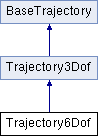
\includegraphics[height=3.000000cm]{group___trajectory}
\end{center}
\end{figure}
\subsubsection*{Public Member Functions}
\begin{DoxyCompactItemize}
\item 
\mbox{\Hypertarget{group___trajectory_ae424fdbe7ec9a60925931a97277975b2}\label{group___trajectory_ae424fdbe7ec9a60925931a97277975b2}} 
virtual void {\bfseries init\+Trajectory} (Aerodynamic\+Struct \&Aero\+Data, Airframe\+Struct \&Airframe\+Data, Thrust\+Struct \&Thrust\+Data, Aircraft\+Struct \&Aircraft\+Data, Guidance\+Struct \&Guidance\+Data)
\item 
\mbox{\Hypertarget{group___trajectory_adb081d9287f12b50ccf60cc894dead4b}\label{group___trajectory_adb081d9287f12b50ccf60cc894dead4b}} 
virtual void {\bfseries update\+Trajectory} (\hyperlink{group___tools_ga3f1431cb9f76da10f59246d1d743dc2c}{Float64} Flight\+Time, Atmosphere\+Struct \&Atmo\+Data, Aerodynamic\+Struct \&Aero\+Data, Airframe\+Struct \&Airframe\+Data, Thrust\+Struct \&Thrust\+Data, Guidance\+Struct \&Guidance\+Data)
\end{DoxyCompactItemize}
\index{Trajectory@{Trajectory}}\label{class_trajectory}
\Hypertarget{group___trajectory_class_trajectory}
\subsubsection{class Trajectory}


Definition at line \hyperlink{_trajectory_8h_source_l00017}{17} of file \hyperlink{_trajectory_8h_source}{Trajectory.\+h}.

\subsubsection*{Public Member Functions}
\begin{DoxyCompactItemize}
\item 
{\bfseries Trajectory} (Sim\+D\+Preference \&Sim\+Pref)
\item 
void {\bfseries select\+Trajectory} (int type)
\item 
void {\bfseries update\+Trajectory} (\hyperlink{group___tools_ga3f1431cb9f76da10f59246d1d743dc2c}{Float64} Flight\+Time, Atmosphere\+Struct \&Atmo\+Data, Aerodynamic\+Struct \&Aero\+Data, Airframe\+Struct \&Airframe\+Data, Thrust\+Struct \&Thrust\+Data, Guidance\+Struct \&Guidance\+Data)
\item 
void {\bfseries init\+Trajectory} (Aerodynamic\+Struct \&Aero\+Data, Airframe\+Struct \&Airframe\+Data, Thrust\+Struct \&Thrust\+Data, Aircraft\+Struct \&Aircraft\+Data, Guidance\+Struct \&Guidance\+Data)
\end{DoxyCompactItemize}
\index{Trajectory3\+Dof@{Trajectory3\+Dof}}\label{class_trajectory3_dof}
\Hypertarget{group___trajectory_class_trajectory3_dof}
\subsubsection{class Trajectory3\+Dof}


Definition at line \hyperlink{_trajectory3_do_f_8h_source_l00019}{19} of file \hyperlink{_trajectory3_do_f_8h_source}{Trajectory3\+Do\+F.\+h}.

Inheritance diagram for Trajectory3\+Dof\+:\begin{figure}[H]
\begin{center}
\leavevmode
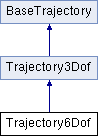
\includegraphics[height=3.000000cm]{group___trajectory}
\end{center}
\end{figure}
\subsubsection*{Public Member Functions}
\begin{DoxyCompactItemize}
\item 
virtual void {\bfseries init\+Trajectory} (Aerodynamic\+Struct \&Aero\+Data, Airframe\+Struct \&Airframe\+Data, Thrust\+Struct \&Thrust\+Data, Aircraft\+Struct \&Aircraft\+Data, Guidance\+Struct \&Guidance\+Data)
\item 
virtual void {\bfseries update\+Trajectory} (\hyperlink{group___tools_ga3f1431cb9f76da10f59246d1d743dc2c}{Float64} Flight\+Time, Atmosphere\+Struct \&Atmo\+Data, Aerodynamic\+Struct \&Aero\+Data, Airframe\+Struct \&Airframe\+Data, Thrust\+Struct \&Thrust\+Data, Guidance\+Struct \&Guidance\+Data)
\item 
void {\bfseries init\+Trajectory3\+DoF} (Aerodynamic\+Struct \&Aero\+Data, Airframe\+Struct \&Airframe\+Data, Thrust\+Struct \&Thrust\+Data, Aircraft\+Struct \&Aircraft\+Data, Guidance\+Struct \&Guidance\+Data)
\item 
void {\bfseries update\+Trajectory3\+DoF} (\hyperlink{group___tools_ga3f1431cb9f76da10f59246d1d743dc2c}{Float64} Flight\+Time, Atmosphere\+Struct \&Atmo\+Data, Aerodynamic\+Struct \&Aero\+Data, Airframe\+Struct \&Airframe\+Data, Thrust\+Struct \&Thrust\+Data, Guidance\+Struct \&Guidance\+Data)
\end{DoxyCompactItemize}
\subsubsection*{Protected Attributes}
\begin{DoxyCompactItemize}
\item 
\hyperlink{group___airframe_class_airframe}{Airframe} $\ast$ {\bfseries airframe}
\end{DoxyCompactItemize}
\index{Trajectory6\+Dof@{Trajectory6\+Dof}}\label{class_trajectory6_dof}
\Hypertarget{group___trajectory_class_trajectory6_dof}
\subsubsection{class Trajectory6\+Dof}


Definition at line \hyperlink{_trajectory6_do_f_8h_source_l00022}{22} of file \hyperlink{_trajectory6_do_f_8h_source}{Trajectory6\+Do\+F.\+h}.

Inheritance diagram for Trajectory6\+Dof\+:\begin{figure}[H]
\begin{center}
\leavevmode
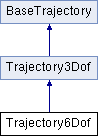
\includegraphics[height=3.000000cm]{group___trajectory}
\end{center}
\end{figure}
\subsubsection*{Public Member Functions}
\begin{DoxyCompactItemize}
\item 
virtual void {\bfseries init\+Trajectory} (Aerodynamic\+Struct \&Aero\+Data, Airframe\+Struct \&Airframe\+Data, Thrust\+Struct \&Thrust\+Data, Aircraft\+Struct \&Aircraft\+Data, Guidance\+Struct \&Guidance\+Data)
\item 
virtual void {\bfseries update\+Trajectory} (\hyperlink{group___tools_ga3f1431cb9f76da10f59246d1d743dc2c}{Float64} Flight\+Time, Atmosphere\+Struct \&Atmo\+Data, Aerodynamic\+Struct \&Aero\+Data, Airframe\+Struct \&Airframe\+Data, Thrust\+Struct \&Thrust\+Data, Guidance\+Struct \&Guidance\+Data)
\end{DoxyCompactItemize}
\subsection*{Additional Inherited Members}

\chapter{Namespace Documentation}
\hypertarget{namespace_unit_test1}{}\section{Unit\+Test1 Namespace Reference}
\label{namespace_unit_test1}\index{Unit\+Test1@{Unit\+Test1}}
\subsection*{Functions}
\begin{DoxyCompactItemize}
\item 
\hyperlink{namespace_unit_test1_a72947bdb044a2f5ee054fe1c31e79255}{T\+E\+S\+T\+\_\+\+C\+L\+A\+SS} (Unit\+Test1)
\end{DoxyCompactItemize}


\subsection{Function Documentation}
\mbox{\Hypertarget{namespace_unit_test1_a72947bdb044a2f5ee054fe1c31e79255}\label{namespace_unit_test1_a72947bdb044a2f5ee054fe1c31e79255}} 
\index{Unit\+Test1@{Unit\+Test1}!T\+E\+S\+T\+\_\+\+C\+L\+A\+SS@{T\+E\+S\+T\+\_\+\+C\+L\+A\+SS}}
\index{T\+E\+S\+T\+\_\+\+C\+L\+A\+SS@{T\+E\+S\+T\+\_\+\+C\+L\+A\+SS}!Unit\+Test1@{Unit\+Test1}}
\subsubsection{\texorpdfstring{T\+E\+S\+T\+\_\+\+C\+L\+A\+S\+S()}{TEST\_CLASS()}}
{\footnotesize\ttfamily Unit\+Test1\+::\+T\+E\+S\+T\+\_\+\+C\+L\+A\+SS (\begin{DoxyParamCaption}\item[{Unit\+Test1}]{ }\end{DoxyParamCaption})}



Definition at line 18 of file unittest1.\+cpp.


\chapter{Class Documentation}
\hypertarget{classacc_table}{}\section{acc\+Table Class Reference}
\label{classacc_table}\index{acc\+Table@{acc\+Table}}
Inheritance diagram for acc\+Table\+:\begin{figure}[H]
\begin{center}
\leavevmode
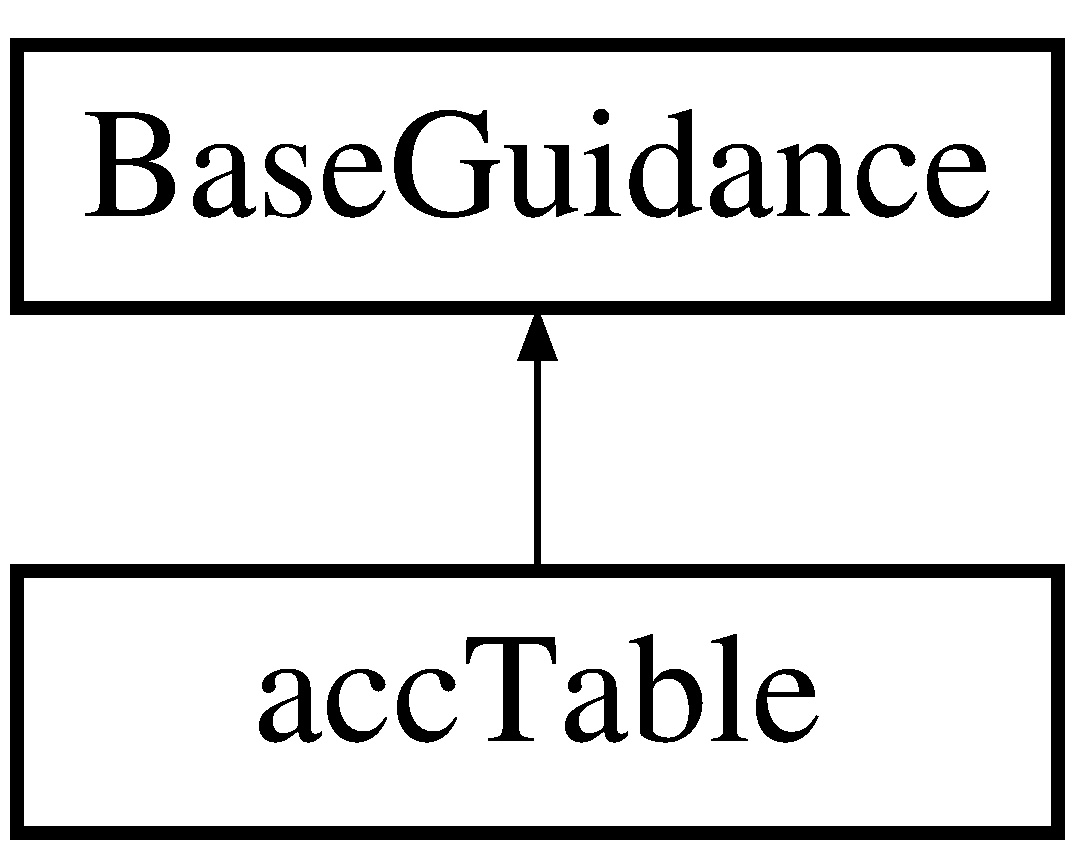
\includegraphics[height=2.000000cm]{classacc_table}
\end{center}
\end{figure}
\subsection*{Public Member Functions}
\begin{DoxyCompactItemize}
\item 
\mbox{\Hypertarget{classacc_table_acccff68d7c26403ed326b2c487fd80ed}\label{classacc_table_acccff68d7c26403ed326b2c487fd80ed}} 
void {\bfseries init\+Guidance} ()
\item 
\mbox{\Hypertarget{classacc_table_a60a9fdb7b041cd5aae020c4a5d252fba}\label{classacc_table_a60a9fdb7b041cd5aae020c4a5d252fba}} 
void {\bfseries update\+Guidance} (\hyperlink{group___tools_ga3f1431cb9f76da10f59246d1d743dc2c}{Float64} Flight\+Time, Aerodynamic\+Struct \&Aero\+Data, Thrust\+Struct \&Thrust\+Data, Airframe\+Struct \&Airframe\+Data, Guidance\+Struct \&Guidance\+Data)
\end{DoxyCompactItemize}


\subsection{Detailed Description}


Definition at line \hyperlink{acc_table_8h_source_l00012}{12} of file \hyperlink{acc_table_8h_source}{acc\+Table.\+h}.



The documentation for this class was generated from the following files\+:\begin{DoxyCompactItemize}
\item 
acc\+Table.\+h\item 
acc\+Table.\+cpp\end{DoxyCompactItemize}

\hypertarget{class_actuator}{}\section{Actuator Class Reference}
\label{class_actuator}\index{Actuator@{Actuator}}


{\ttfamily \#include $<$Actuator.\+h$>$}

\subsection*{Public Member Functions}
\begin{DoxyCompactItemize}
\item 
\hyperlink{class_actuator_a136af3d7d681d8c445e5d4ce552e4741}{Actuator} (Sim\+D\+Preference \&Sim\+Pref)
\begin{DoxyCompactList}\small\item\em constructor \end{DoxyCompactList}\item 
\hyperlink{class_actuator_a3c19e3031076395a918ab72e1acc8a3c}{$\sim$\+Actuator} ()
\begin{DoxyCompactList}\small\item\em destructor \end{DoxyCompactList}\item 
void \hyperlink{class_actuator_afb76ea4c70afd8dc6c8968be090ee4c5}{init\+Actuator} (\hyperlink{group___tools_ga3f1431cb9f76da10f59246d1d743dc2c}{Float64} \&Flight\+Time, Airframe\+Struct \&Airframe\+Data, Actuator\+Struct \&Actuator\+Data)
\begin{DoxyCompactList}\small\item\em initialize selected actuator model \end{DoxyCompactList}\item 
void \hyperlink{class_actuator_a9276e545f7378225f4efab89014a90a7}{select\+Actuator\+Type} (int type)
\begin{DoxyCompactList}\small\item\em switch function to select desired model \end{DoxyCompactList}\item 
void \hyperlink{class_actuator_a63aacfd84f07a1beb097b117b818c30f}{update\+Actuator} (\hyperlink{group___tools_ga3f1431cb9f76da10f59246d1d743dc2c}{Float64} Flight\+Time, Airframe\+Struct \&Airframe\+Data, Actuator\+Struct \&Actuator\+Data)
\begin{DoxyCompactList}\small\item\em update actuator model \end{DoxyCompactList}\item 
void \hyperlink{class_actuator_a0acfebd90c57b798d6b1136fade21347}{log\+Actuator} ()
\begin{DoxyCompactList}\small\item\em data logger for actuator data \end{DoxyCompactList}\end{DoxyCompactItemize}


\subsection{Detailed Description}


Definition at line 18 of file Actuator.\+h.



\subsection{Constructor \& Destructor Documentation}
\mbox{\Hypertarget{class_actuator_a136af3d7d681d8c445e5d4ce552e4741}\label{class_actuator_a136af3d7d681d8c445e5d4ce552e4741}} 
\index{Actuator@{Actuator}!Actuator@{Actuator}}
\index{Actuator@{Actuator}!Actuator@{Actuator}}
\subsubsection{\texorpdfstring{Actuator()}{Actuator()}}
{\footnotesize\ttfamily Actuator\+::\+Actuator (\begin{DoxyParamCaption}\item[{Sim\+D\+Preference \&}]{Sim\+Pref }\end{DoxyParamCaption})}



constructor 


\begin{DoxyParams}{Parameters}
{\em Sim\+Pref} & Selected \hyperlink{class_actuator}{Actuator} model \\
\hline
\end{DoxyParams}


Definition at line 3 of file Actuator.\+cpp.

\mbox{\Hypertarget{class_actuator_a3c19e3031076395a918ab72e1acc8a3c}\label{class_actuator_a3c19e3031076395a918ab72e1acc8a3c}} 
\index{Actuator@{Actuator}!````~Actuator@{$\sim$\+Actuator}}
\index{````~Actuator@{$\sim$\+Actuator}!Actuator@{Actuator}}
\subsubsection{\texorpdfstring{$\sim$\+Actuator()}{~Actuator()}}
{\footnotesize\ttfamily Actuator\+::$\sim$\+Actuator (\begin{DoxyParamCaption}{ }\end{DoxyParamCaption})}



destructor 



Definition at line 8 of file Actuator.\+cpp.



\subsection{Member Function Documentation}
\mbox{\Hypertarget{class_actuator_afb76ea4c70afd8dc6c8968be090ee4c5}\label{class_actuator_afb76ea4c70afd8dc6c8968be090ee4c5}} 
\index{Actuator@{Actuator}!init\+Actuator@{init\+Actuator}}
\index{init\+Actuator@{init\+Actuator}!Actuator@{Actuator}}
\subsubsection{\texorpdfstring{init\+Actuator()}{initActuator()}}
{\footnotesize\ttfamily void Actuator\+::init\+Actuator (\begin{DoxyParamCaption}\item[{\hyperlink{group___tools_ga3f1431cb9f76da10f59246d1d743dc2c}{Float64} \&}]{Flight\+Time,  }\item[{Airframe\+Struct \&}]{Airframe\+Data,  }\item[{Actuator\+Struct \&}]{Actuator\+Data }\end{DoxyParamCaption})}



initialize selected actuator model 


\begin{DoxyParams}{Parameters}
{\em Flight\+Time} & Flight time \\
\hline
{\em Airframe\+Data} & coammanded actuator angles from autopilot \\
\hline
{\em Actuator\+Data} & real \hyperlink{class_actuator}{Actuator} angles \\
\hline
\end{DoxyParams}


Definition at line 12 of file Actuator.\+cpp.



Referenced by Real\+System\+Trajectory\+::init\+Trajectory().

\mbox{\Hypertarget{class_actuator_a0acfebd90c57b798d6b1136fade21347}\label{class_actuator_a0acfebd90c57b798d6b1136fade21347}} 
\index{Actuator@{Actuator}!log\+Actuator@{log\+Actuator}}
\index{log\+Actuator@{log\+Actuator}!Actuator@{Actuator}}
\subsubsection{\texorpdfstring{log\+Actuator()}{logActuator()}}
{\footnotesize\ttfamily void Actuator\+::log\+Actuator (\begin{DoxyParamCaption}{ }\end{DoxyParamCaption})}



data logger for actuator data 



Definition at line 42 of file Actuator.\+cpp.



Referenced by Real\+System\+Trajectory\+::log\+Realsystem\+Trajectory().

\mbox{\Hypertarget{class_actuator_a9276e545f7378225f4efab89014a90a7}\label{class_actuator_a9276e545f7378225f4efab89014a90a7}} 
\index{Actuator@{Actuator}!select\+Actuator\+Type@{select\+Actuator\+Type}}
\index{select\+Actuator\+Type@{select\+Actuator\+Type}!Actuator@{Actuator}}
\subsubsection{\texorpdfstring{select\+Actuator\+Type()}{selectActuatorType()}}
{\footnotesize\ttfamily void Actuator\+::select\+Actuator\+Type (\begin{DoxyParamCaption}\item[{int}]{type }\end{DoxyParamCaption})}



switch function to select desired model 


\begin{DoxyParams}{Parameters}
{\em type} & selected model (as integer value9 \\
\hline
\end{DoxyParams}


Definition at line 21 of file Actuator.\+cpp.



Referenced by Actuator().

\mbox{\Hypertarget{class_actuator_a63aacfd84f07a1beb097b117b818c30f}\label{class_actuator_a63aacfd84f07a1beb097b117b818c30f}} 
\index{Actuator@{Actuator}!update\+Actuator@{update\+Actuator}}
\index{update\+Actuator@{update\+Actuator}!Actuator@{Actuator}}
\subsubsection{\texorpdfstring{update\+Actuator()}{updateActuator()}}
{\footnotesize\ttfamily void Actuator\+::update\+Actuator (\begin{DoxyParamCaption}\item[{\hyperlink{group___tools_ga3f1431cb9f76da10f59246d1d743dc2c}{Float64}}]{Flight\+Time,  }\item[{Airframe\+Struct \&}]{Airframe\+Data,  }\item[{Actuator\+Struct \&}]{Actuator\+Data }\end{DoxyParamCaption})}



update actuator model 


\begin{DoxyParams}{Parameters}
{\em Flight\+Time} & Flight time \\
\hline
{\em Airframe\+Data} & coammanded actuator angles from autopilot \\
\hline
{\em Actuator\+Data} & real \hyperlink{class_actuator}{Actuator} angles \\
\hline
\end{DoxyParams}


Definition at line 32 of file Actuator.\+cpp.



Referenced by Real\+System\+Trajectory\+::update\+Trajectory().



The documentation for this class was generated from the following files\+:\begin{DoxyCompactItemize}
\item 
C\+:/\+Users/janol/\+Desktop/\+Simulation\+\_\+\+Stand230618/\+Actuator/\hyperlink{_actuator_8h}{Actuator.\+h}\item 
C\+:/\+Users/janol/\+Desktop/\+Simulation\+\_\+\+Stand230618/\+Actuator/\hyperlink{_actuator_8cpp}{Actuator.\+cpp}\end{DoxyCompactItemize}

\hypertarget{class_aerodynamics}{}\section{Aerodynamics Class Reference}
\label{class_aerodynamics}\index{Aerodynamics@{Aerodynamics}}


{\ttfamily \#include $<$Aerodynamic.\+h$>$}

\subsection*{Public Member Functions}
\begin{DoxyCompactItemize}
\item 
\hyperlink{class_aerodynamics_af0582a3e010d9614ace4b96f31fc2a8d}{Aerodynamics} (Sim\+D\+Preference \&Sim\+Pref)
\begin{DoxyCompactList}\small\item\em constructor \end{DoxyCompactList}\item 
\hyperlink{class_aerodynamics_af0e048e0c80ec8334997b79b761fea60}{$\sim$\+Aerodynamics} ()
\begin{DoxyCompactList}\small\item\em destructor \end{DoxyCompactList}\item 
void \hyperlink{class_aerodynamics_a9aa3397e8b1d91ed237146a57bbe6bcf}{select\+Aerodynamic\+Type} (int type)
\begin{DoxyCompactList}\small\item\em set pointer to desired class \end{DoxyCompactList}\item 
void \hyperlink{class_aerodynamics_a9970a48140e0d956f6e0cc5f6d5cda33}{init\+Aerodynamic} (\hyperlink{group___tools_ga3f1431cb9f76da10f59246d1d743dc2c}{Float64} \&Flight\+Time, Aerodynamic\+Struct \&Aero\+Data, Aircraft\+Struct \&Aircraft\+Data)
\begin{DoxyCompactList}\small\item\em initialize aerodynamic paramters \end{DoxyCompactList}\item 
void \hyperlink{class_aerodynamics_a83f9967d09e40e6c53dd17815f6bb096}{update\+Aerodynamic} (\hyperlink{group___tools_ga3f1431cb9f76da10f59246d1d743dc2c}{Float64} Flight\+Time, Atmosphere\+Struct \&Atmo\+Data, Aerodynamic\+Struct \&Aero\+Data, Airframe\+Struct \&Airframe\+Data, Thrust\+Struct \&Thrust\+Data, Actuator\+Struct \&Actuator\+Data, I\+M\+U\+Struct \&I\+M\+U\+Data, Navigation\+Struct \&Nav\+Data)
\begin{DoxyCompactList}\small\item\em calculate aero forces and moments \end{DoxyCompactList}\item 
void \hyperlink{class_aerodynamics_aa7af099a965b08deb4e86753149522e9}{Log\+Aero\+Data} ()
\begin{DoxyCompactList}\small\item\em log aerodynamic data to text file \end{DoxyCompactList}\end{DoxyCompactItemize}


\subsection{Detailed Description}


Definition at line 22 of file Aerodynamic.\+h.



\subsection{Constructor \& Destructor Documentation}
\mbox{\Hypertarget{class_aerodynamics_af0582a3e010d9614ace4b96f31fc2a8d}\label{class_aerodynamics_af0582a3e010d9614ace4b96f31fc2a8d}} 
\index{Aerodynamics@{Aerodynamics}!Aerodynamics@{Aerodynamics}}
\index{Aerodynamics@{Aerodynamics}!Aerodynamics@{Aerodynamics}}
\subsubsection{\texorpdfstring{Aerodynamics()}{Aerodynamics()}}
{\footnotesize\ttfamily Aerodynamics\+::\+Aerodynamics (\begin{DoxyParamCaption}\item[{Sim\+D\+Preference \&}]{Sim\+Pref }\end{DoxyParamCaption})}



constructor 


\begin{DoxyParams}{Parameters}
{\em Sim\+Pref} & structure of model selctions \\
\hline
\end{DoxyParams}


Definition at line 3 of file Aerodynamic.\+cpp.

\mbox{\Hypertarget{class_aerodynamics_af0e048e0c80ec8334997b79b761fea60}\label{class_aerodynamics_af0e048e0c80ec8334997b79b761fea60}} 
\index{Aerodynamics@{Aerodynamics}!````~Aerodynamics@{$\sim$\+Aerodynamics}}
\index{````~Aerodynamics@{$\sim$\+Aerodynamics}!Aerodynamics@{Aerodynamics}}
\subsubsection{\texorpdfstring{$\sim$\+Aerodynamics()}{~Aerodynamics()}}
{\footnotesize\ttfamily Aerodynamics\+::$\sim$\+Aerodynamics (\begin{DoxyParamCaption}{ }\end{DoxyParamCaption})}



destructor 



Definition at line 9 of file Aerodynamic.\+cpp.



\subsection{Member Function Documentation}
\mbox{\Hypertarget{class_aerodynamics_a9970a48140e0d956f6e0cc5f6d5cda33}\label{class_aerodynamics_a9970a48140e0d956f6e0cc5f6d5cda33}} 
\index{Aerodynamics@{Aerodynamics}!init\+Aerodynamic@{init\+Aerodynamic}}
\index{init\+Aerodynamic@{init\+Aerodynamic}!Aerodynamics@{Aerodynamics}}
\subsubsection{\texorpdfstring{init\+Aerodynamic()}{initAerodynamic()}}
{\footnotesize\ttfamily void Aerodynamics\+::init\+Aerodynamic (\begin{DoxyParamCaption}\item[{\hyperlink{group___tools_ga3f1431cb9f76da10f59246d1d743dc2c}{Float64} \&}]{Flight\+Time,  }\item[{Aerodynamic\+Struct \&}]{Aero\+Data,  }\item[{Aircraft\+Struct \&}]{Aircraft\+Data }\end{DoxyParamCaption})}



initialize aerodynamic paramters 


\begin{DoxyParams}{Parameters}
{\em Flight\+Time} & flighttime \\
\hline
{\em Aero\+Data} & structure of aero data \\
\hline
{\em Aircraft\+Data} & structure of aircraft data \\
\hline
\end{DoxyParams}


Definition at line 24 of file Aerodynamic.\+cpp.



Referenced by Aerodynamic\+Test(), Guidance\+Test(), and Trajectory3\+Dof\+::init\+Trajectory3\+Do\+F().

\mbox{\Hypertarget{class_aerodynamics_aa7af099a965b08deb4e86753149522e9}\label{class_aerodynamics_aa7af099a965b08deb4e86753149522e9}} 
\index{Aerodynamics@{Aerodynamics}!Log\+Aero\+Data@{Log\+Aero\+Data}}
\index{Log\+Aero\+Data@{Log\+Aero\+Data}!Aerodynamics@{Aerodynamics}}
\subsubsection{\texorpdfstring{Log\+Aero\+Data()}{LogAeroData()}}
{\footnotesize\ttfamily void Aerodynamics\+::\+Log\+Aero\+Data (\begin{DoxyParamCaption}{ }\end{DoxyParamCaption})}



log aerodynamic data to text file 



Definition at line 53 of file Aerodynamic.\+cpp.



Referenced by Trajectory3\+Dof\+::log3\+Dof\+Data().

\mbox{\Hypertarget{class_aerodynamics_a9aa3397e8b1d91ed237146a57bbe6bcf}\label{class_aerodynamics_a9aa3397e8b1d91ed237146a57bbe6bcf}} 
\index{Aerodynamics@{Aerodynamics}!select\+Aerodynamic\+Type@{select\+Aerodynamic\+Type}}
\index{select\+Aerodynamic\+Type@{select\+Aerodynamic\+Type}!Aerodynamics@{Aerodynamics}}
\subsubsection{\texorpdfstring{select\+Aerodynamic\+Type()}{selectAerodynamicType()}}
{\footnotesize\ttfamily void Aerodynamics\+::select\+Aerodynamic\+Type (\begin{DoxyParamCaption}\item[{int}]{type }\end{DoxyParamCaption})}



set pointer to desired class 


\begin{DoxyParams}{Parameters}
{\em type} & Aerodynamic Model Selection \\
\hline
\end{DoxyParams}


Definition at line 13 of file Aerodynamic.\+cpp.



Referenced by Aerodynamics().

\mbox{\Hypertarget{class_aerodynamics_a83f9967d09e40e6c53dd17815f6bb096}\label{class_aerodynamics_a83f9967d09e40e6c53dd17815f6bb096}} 
\index{Aerodynamics@{Aerodynamics}!update\+Aerodynamic@{update\+Aerodynamic}}
\index{update\+Aerodynamic@{update\+Aerodynamic}!Aerodynamics@{Aerodynamics}}
\subsubsection{\texorpdfstring{update\+Aerodynamic()}{updateAerodynamic()}}
{\footnotesize\ttfamily void Aerodynamics\+::update\+Aerodynamic (\begin{DoxyParamCaption}\item[{\hyperlink{group___tools_ga3f1431cb9f76da10f59246d1d743dc2c}{Float64}}]{Flight\+Time,  }\item[{Atmosphere\+Struct \&}]{Atmo\+Data,  }\item[{Aerodynamic\+Struct \&}]{Aero\+Data,  }\item[{Airframe\+Struct \&}]{Airframe\+Data,  }\item[{Thrust\+Struct \&}]{Thrust\+Data,  }\item[{Actuator\+Struct \&}]{Actuator\+Data,  }\item[{I\+M\+U\+Struct \&}]{I\+M\+U\+Data,  }\item[{Navigation\+Struct \&}]{Nav\+Data }\end{DoxyParamCaption})}



calculate aero forces and moments 


\begin{DoxyParams}{Parameters}
{\em Flight\+Time} & Flight Time \\
\hline
{\em Atmo\+Data} & air density, speed of sound \\
\hline
{\em Aero\+Data} & structure of aero data \\
\hline
{\em Airframe\+Data} & structure of airframe data \\
\hline
{\em Thrust\+Data} & structure of thrust data \\
\hline
{\em Actuator\+Data} & actuator angles \\
\hline
{\em I\+M\+U\+Data} & rotational rates \\
\hline
{\em Nav\+Data} & \hyperlink{class_navigation}{Navigation} data like velocity in N\+ED system \\
\hline
\end{DoxyParams}


Definition at line 33 of file Aerodynamic.\+cpp.



Referenced by Aerodynamic\+Test(), Guidance\+Test(), and Trajectory3\+Dof\+::update\+Trajectory3\+Do\+F().



The documentation for this class was generated from the following files\+:\begin{DoxyCompactItemize}
\item 
C\+:/\+Users/janol/\+Desktop/\+Simulation\+\_\+\+Stand230618/\+Aerodynamic/\hyperlink{_aerodynamic_8h}{Aerodynamic.\+h}\item 
C\+:/\+Users/janol/\+Desktop/\+Simulation\+\_\+\+Stand230618/\+Aerodynamic/\hyperlink{_aerodynamic_8cpp}{Aerodynamic.\+cpp}\end{DoxyCompactItemize}

\hypertarget{class_aircraft}{}\section{Aircraft Class Reference}
\label{class_aircraft}\index{Aircraft@{Aircraft}}
\subsection*{Public Member Functions}
\begin{DoxyCompactItemize}
\item 
\mbox{\Hypertarget{class_aircraft_ae4436b1de6bdf2702816643fc787c4ec}\label{class_aircraft_ae4436b1de6bdf2702816643fc787c4ec}} 
void {\bfseries init\+Aircraft} ()
\item 
\mbox{\Hypertarget{class_aircraft_afc4b47817c55b981e41c7e6cecdb80df}\label{class_aircraft_afc4b47817c55b981e41c7e6cecdb80df}} 
void {\bfseries simulate\+Aircraft} ()
\end{DoxyCompactItemize}


\subsection{Detailed Description}


Definition at line \hyperlink{_aircraft_8h_source_l00005}{5} of file \hyperlink{_aircraft_8h_source}{Aircraft.\+h}.



The documentation for this class was generated from the following files\+:\begin{DoxyCompactItemize}
\item 
Aircraft.\+h\item 
Aircraft.\+cpp\end{DoxyCompactItemize}

\hypertarget{class_airframe}{}\section{Airframe Class Reference}
\label{class_airframe}\index{Airframe@{Airframe}}


{\ttfamily \#include $<$Airframe.\+h$>$}

\subsection*{Public Member Functions}
\begin{DoxyCompactItemize}
\item 
\hyperlink{class_airframe_a5e6632c7d0c5bc5b889de6cc2407944f}{Airframe} ()
\begin{DoxyCompactList}\small\item\em constructor \end{DoxyCompactList}\item 
\hyperlink{class_airframe_af849116afbf7c4d7d2d5c189ff68cb7d}{$\sim$\+Airframe} ()
\begin{DoxyCompactList}\small\item\em destructor \end{DoxyCompactList}\item 
void \hyperlink{class_airframe_ad7e530da939683d17010262d0fee76ca}{init\+Airframe} (\hyperlink{group___tools_ga3f1431cb9f76da10f59246d1d743dc2c}{Float64} \&Flight\+Time, Aircraft\+Struct \&Aircraft\+Data, Airframe\+Struct \&Airframe\+Data)
\begin{DoxyCompactList}\small\item\em \hyperlink{class_airframe}{Airframe} initialization \hyperlink{class_airframe}{Airframe} and \hyperlink{class_aircraft}{Aircraft} Data are initialized. Parameters from Aircraft.\+dat are read in and stored in their specific structure. \end{DoxyCompactList}\item 
void \hyperlink{class_airframe_a29b3a2854700f77468b6a94c5b7d0372}{update\+Translational} (Aerodynamic\+Struct \&Aero\+Data, Thrust\+Struct \&Thrust\+Data, Airframe\+Struct \&Airframe\+Data)
\begin{DoxyCompactList}\small\item\em translational equations of motion translational body accelerations are calculated \end{DoxyCompactList}\item 
void \hyperlink{class_airframe_a93b66b243b961518c207192c912cc6f2}{update\+Rotatory} (Aerodynamic\+Struct \&Aero\+Data, Thrust\+Struct \&Thrust\+Data, Airframe\+Struct \&Airframe\+Data)
\begin{DoxyCompactList}\small\item\em rotational equations of motion rotation body accelerations are calculated. Euler angle derivatives,too. \end{DoxyCompactList}\item 
void \hyperlink{class_airframe_ac1c2c7b3b51e6780b544e4df897cb585}{init\+Log\+Airframe\+Data} (\hyperlink{group___tools_ga3f1431cb9f76da10f59246d1d743dc2c}{Float64} \&Flight\+Time, Airframe\+Struct \&Airframe\+Data)
\begin{DoxyCompactList}\small\item\em define output \end{DoxyCompactList}\item 
void \hyperlink{class_airframe_ab5b3c30a5d3d6d5e89b3dfdd0dbd14e4}{log\+Airframe\+Data} ()
\begin{DoxyCompactList}\small\item\em log airframe data \end{DoxyCompactList}\end{DoxyCompactItemize}


\subsection{Detailed Description}


Definition at line 18 of file Airframe.\+h.



\subsection{Constructor \& Destructor Documentation}
\mbox{\Hypertarget{class_airframe_a5e6632c7d0c5bc5b889de6cc2407944f}\label{class_airframe_a5e6632c7d0c5bc5b889de6cc2407944f}} 
\index{Airframe@{Airframe}!Airframe@{Airframe}}
\index{Airframe@{Airframe}!Airframe@{Airframe}}
\subsubsection{\texorpdfstring{Airframe()}{Airframe()}}
{\footnotesize\ttfamily Airframe\+::\+Airframe (\begin{DoxyParamCaption}{ }\end{DoxyParamCaption})}



constructor 



Definition at line 3 of file Airframe.\+cpp.

\mbox{\Hypertarget{class_airframe_af849116afbf7c4d7d2d5c189ff68cb7d}\label{class_airframe_af849116afbf7c4d7d2d5c189ff68cb7d}} 
\index{Airframe@{Airframe}!````~Airframe@{$\sim$\+Airframe}}
\index{````~Airframe@{$\sim$\+Airframe}!Airframe@{Airframe}}
\subsubsection{\texorpdfstring{$\sim$\+Airframe()}{~Airframe()}}
{\footnotesize\ttfamily Airframe\+::$\sim$\+Airframe (\begin{DoxyParamCaption}{ }\end{DoxyParamCaption})}



destructor 



Definition at line 9 of file Airframe.\+cpp.



\subsection{Member Function Documentation}
\mbox{\Hypertarget{class_airframe_ad7e530da939683d17010262d0fee76ca}\label{class_airframe_ad7e530da939683d17010262d0fee76ca}} 
\index{Airframe@{Airframe}!init\+Airframe@{init\+Airframe}}
\index{init\+Airframe@{init\+Airframe}!Airframe@{Airframe}}
\subsubsection{\texorpdfstring{init\+Airframe()}{initAirframe()}}
{\footnotesize\ttfamily void Airframe\+::init\+Airframe (\begin{DoxyParamCaption}\item[{\hyperlink{group___tools_ga3f1431cb9f76da10f59246d1d743dc2c}{Float64} \&}]{Flight\+Time,  }\item[{Aircraft\+Struct \&}]{Aircraft\+Data,  }\item[{Airframe\+Struct \&}]{Airframe\+Data }\end{DoxyParamCaption})}



\hyperlink{class_airframe}{Airframe} initialization \hyperlink{class_airframe}{Airframe} and \hyperlink{class_aircraft}{Aircraft} Data are initialized. Parameters from Aircraft.\+dat are read in and stored in their specific structure. 

1) read in geometric aircraft data (wingspan,...)

3) initialize airframe data 

Definition at line 13 of file Airframe.\+cpp.



Referenced by Trajectory3\+Dof\+::init\+Trajectory3\+Do\+F().

\mbox{\Hypertarget{class_airframe_ac1c2c7b3b51e6780b544e4df897cb585}\label{class_airframe_ac1c2c7b3b51e6780b544e4df897cb585}} 
\index{Airframe@{Airframe}!init\+Log\+Airframe\+Data@{init\+Log\+Airframe\+Data}}
\index{init\+Log\+Airframe\+Data@{init\+Log\+Airframe\+Data}!Airframe@{Airframe}}
\subsubsection{\texorpdfstring{init\+Log\+Airframe\+Data()}{initLogAirframeData()}}
{\footnotesize\ttfamily void Airframe\+::init\+Log\+Airframe\+Data (\begin{DoxyParamCaption}\item[{\hyperlink{group___tools_ga3f1431cb9f76da10f59246d1d743dc2c}{Float64} \&}]{Flight\+Time,  }\item[{Airframe\+Struct \&}]{Airframe\+Data }\end{DoxyParamCaption})}



define output 


\begin{DoxyParams}{Parameters}
{\em Flight\+Time} & flight time \\
\hline
{\em Airframe\+Data} & flight states \\
\hline
\end{DoxyParams}


Definition at line 117 of file Airframe.\+cpp.



Referenced by init\+Airframe().

\mbox{\Hypertarget{class_airframe_ab5b3c30a5d3d6d5e89b3dfdd0dbd14e4}\label{class_airframe_ab5b3c30a5d3d6d5e89b3dfdd0dbd14e4}} 
\index{Airframe@{Airframe}!log\+Airframe\+Data@{log\+Airframe\+Data}}
\index{log\+Airframe\+Data@{log\+Airframe\+Data}!Airframe@{Airframe}}
\subsubsection{\texorpdfstring{log\+Airframe\+Data()}{logAirframeData()}}
{\footnotesize\ttfamily void Airframe\+::log\+Airframe\+Data (\begin{DoxyParamCaption}{ }\end{DoxyParamCaption})}



log airframe data 



Definition at line 126 of file Airframe.\+cpp.



Referenced by Trajectory3\+Dof\+::log3\+Dof\+Data().

\mbox{\Hypertarget{class_airframe_a93b66b243b961518c207192c912cc6f2}\label{class_airframe_a93b66b243b961518c207192c912cc6f2}} 
\index{Airframe@{Airframe}!update\+Rotatory@{update\+Rotatory}}
\index{update\+Rotatory@{update\+Rotatory}!Airframe@{Airframe}}
\subsubsection{\texorpdfstring{update\+Rotatory()}{updateRotatory()}}
{\footnotesize\ttfamily void Airframe\+::update\+Rotatory (\begin{DoxyParamCaption}\item[{Aerodynamic\+Struct \&}]{Aero\+Data,  }\item[{Thrust\+Struct \&}]{Thrust\+Data,  }\item[{Airframe\+Struct \&}]{Airframe\+Data }\end{DoxyParamCaption})}



rotational equations of motion rotation body accelerations are calculated. Euler angle derivatives,too. 


\begin{DoxyParams}{Parameters}
{\em Aero\+Data} & Aerodynamic forces,moments and angles \\
\hline
{\em Thrust\+Data} & Thrust forces and moments \\
\hline
{\em Airframe\+Data} & store accelerations \\
\hline
\end{DoxyParams}
1) get data from structs

2) calculate rotatory accelerations

3) calculate derivation of euler angles 

Definition at line 86 of file Airframe.\+cpp.



Referenced by Real\+System\+Trajectory\+::update\+Trajectory(), and Trajectory6\+Dof\+::update\+Trajectory().

\mbox{\Hypertarget{class_airframe_a29b3a2854700f77468b6a94c5b7d0372}\label{class_airframe_a29b3a2854700f77468b6a94c5b7d0372}} 
\index{Airframe@{Airframe}!update\+Translational@{update\+Translational}}
\index{update\+Translational@{update\+Translational}!Airframe@{Airframe}}
\subsubsection{\texorpdfstring{update\+Translational()}{updateTranslational()}}
{\footnotesize\ttfamily void Airframe\+::update\+Translational (\begin{DoxyParamCaption}\item[{Aerodynamic\+Struct \&}]{Aero\+Data,  }\item[{Thrust\+Struct \&}]{Thrust\+Data,  }\item[{Airframe\+Struct \&}]{Airframe\+Data }\end{DoxyParamCaption})}



translational equations of motion translational body accelerations are calculated 


\begin{DoxyParams}{Parameters}
{\em Aero\+Data} & Aerodynamic forces,moments and angles \\
\hline
{\em Thrust\+Data} & Thrust forces and moments \\
\hline
{\em Airframe\+Data} & store acceleration \\
\hline
\end{DoxyParams}
1) get data from structs

2) calculate translational accelerations 

Definition at line 64 of file Airframe.\+cpp.



Referenced by Trajectory3\+Dof\+::update\+Trajectory3\+Do\+F().



The documentation for this class was generated from the following files\+:\begin{DoxyCompactItemize}
\item 
C\+:/\+Users/janol/\+Desktop/\+Simulation\+\_\+\+Stand230618/\+Airframe/\hyperlink{_airframe_8h}{Airframe.\+h}\item 
C\+:/\+Users/janol/\+Desktop/\+Simulation\+\_\+\+Stand230618/\+Airframe/\hyperlink{_airframe_8cpp}{Airframe.\+cpp}\end{DoxyCompactItemize}

\hypertarget{class_atmopshere}{}\section{Atmopshere Class Reference}
\label{class_atmopshere}\index{Atmopshere@{Atmopshere}}
\subsection*{Public Member Functions}
\begin{DoxyCompactItemize}
\item 
\mbox{\Hypertarget{class_atmopshere_a6e1d5763fbb6631784c99ee3c88911bd}\label{class_atmopshere_a6e1d5763fbb6631784c99ee3c88911bd}} 
void {\bfseries init\+Atmosphere} ()
\item 
\mbox{\Hypertarget{class_atmopshere_a2bd97471d32725d6196ee6816ea36c99}\label{class_atmopshere_a2bd97471d32725d6196ee6816ea36c99}} 
void {\bfseries update\+Atmosphere} (Float64 \&Altitude, \hyperlink{group___data_cloud_struct_atmosphere_struct}{Atmosphere\+Struct} \&Atmo\+Data)
\end{DoxyCompactItemize}


The documentation for this class was generated from the following files\+:\begin{DoxyCompactItemize}
\item 
Atmosphere.\+h\item 
Atmosphere.\+cpp\end{DoxyCompactItemize}

\hypertarget{class_autopilot}{}\section{Autopilot Class Reference}
\label{class_autopilot}\index{Autopilot@{Autopilot}}


{\ttfamily \#include $<$Autopilot.\+h$>$}

\subsection*{Public Member Functions}
\begin{DoxyCompactItemize}
\item 
\hyperlink{class_autopilot_a7687901ca400c7f1bd0e1a05cfb8e689}{Autopilot} ()
\begin{DoxyCompactList}\small\item\em constructor \end{DoxyCompactList}\item 
\hyperlink{class_autopilot_a5e0044bf8d2f51f800486ab7e5c2534d}{$\sim$\+Autopilot} ()
\begin{DoxyCompactList}\small\item\em destructor \end{DoxyCompactList}\item 
void \hyperlink{class_autopilot_aea3535a0804c6ae837c737298eaed687}{init\+Autopilot} ()
\begin{DoxyCompactList}\small\item\em initialize autopilot \end{DoxyCompactList}\item 
void \hyperlink{class_autopilot_aa465fd6235f0a8787dee18a9b33c1a40}{update\+Autopilot} (\hyperlink{group___tools_ga3f1431cb9f76da10f59246d1d743dc2c}{Float64} Flight\+Time, Airframe\+Struct \&Airframe\+Data, Aerodynamic\+Struct \&Aero\+Data, Guidance\+Struct \&Guidance\+Data, Actuator\+Struct \&Actuator\+Data, I\+M\+U\+Struct \&I\+M\+U\+Data, Navigation\+Struct \&Nav\+Data)
\begin{DoxyCompactList}\small\item\em calculate controlls \end{DoxyCompactList}\end{DoxyCompactItemize}


\subsection{Detailed Description}


Definition at line 18 of file Autopilot.\+h.



\subsection{Constructor \& Destructor Documentation}
\mbox{\Hypertarget{class_autopilot_a7687901ca400c7f1bd0e1a05cfb8e689}\label{class_autopilot_a7687901ca400c7f1bd0e1a05cfb8e689}} 
\index{Autopilot@{Autopilot}!Autopilot@{Autopilot}}
\index{Autopilot@{Autopilot}!Autopilot@{Autopilot}}
\subsubsection{\texorpdfstring{Autopilot()}{Autopilot()}}
{\footnotesize\ttfamily Autopilot\+::\+Autopilot (\begin{DoxyParamCaption}{ }\end{DoxyParamCaption})}



constructor 



Definition at line 3 of file Autopilot.\+cpp.

\mbox{\Hypertarget{class_autopilot_a5e0044bf8d2f51f800486ab7e5c2534d}\label{class_autopilot_a5e0044bf8d2f51f800486ab7e5c2534d}} 
\index{Autopilot@{Autopilot}!````~Autopilot@{$\sim$\+Autopilot}}
\index{````~Autopilot@{$\sim$\+Autopilot}!Autopilot@{Autopilot}}
\subsubsection{\texorpdfstring{$\sim$\+Autopilot()}{~Autopilot()}}
{\footnotesize\ttfamily Autopilot\+::$\sim$\+Autopilot (\begin{DoxyParamCaption}{ }\end{DoxyParamCaption})}



destructor 



Definition at line 8 of file Autopilot.\+cpp.



\subsection{Member Function Documentation}
\mbox{\Hypertarget{class_autopilot_aea3535a0804c6ae837c737298eaed687}\label{class_autopilot_aea3535a0804c6ae837c737298eaed687}} 
\index{Autopilot@{Autopilot}!init\+Autopilot@{init\+Autopilot}}
\index{init\+Autopilot@{init\+Autopilot}!Autopilot@{Autopilot}}
\subsubsection{\texorpdfstring{init\+Autopilot()}{initAutopilot()}}
{\footnotesize\ttfamily void Autopilot\+::init\+Autopilot (\begin{DoxyParamCaption}{ }\end{DoxyParamCaption})}



initialize autopilot 



Definition at line 13 of file Autopilot.\+cpp.



Referenced by Real\+System\+Trajectory\+::init\+Trajectory(), and Trajectory6\+Dof\+::init\+Trajectory().

\mbox{\Hypertarget{class_autopilot_aa465fd6235f0a8787dee18a9b33c1a40}\label{class_autopilot_aa465fd6235f0a8787dee18a9b33c1a40}} 
\index{Autopilot@{Autopilot}!update\+Autopilot@{update\+Autopilot}}
\index{update\+Autopilot@{update\+Autopilot}!Autopilot@{Autopilot}}
\subsubsection{\texorpdfstring{update\+Autopilot()}{updateAutopilot()}}
{\footnotesize\ttfamily void Autopilot\+::update\+Autopilot (\begin{DoxyParamCaption}\item[{\hyperlink{group___tools_ga3f1431cb9f76da10f59246d1d743dc2c}{Float64}}]{Flight\+Time,  }\item[{Airframe\+Struct \&}]{Airframe\+Data,  }\item[{Aerodynamic\+Struct \&}]{Aero\+Data,  }\item[{Guidance\+Struct \&}]{Guidance\+Data,  }\item[{Actuator\+Struct \&}]{Actuator\+Data,  }\item[{I\+M\+U\+Struct \&}]{I\+M\+U\+Data,  }\item[{Navigation\+Struct \&}]{Nav\+Data }\end{DoxyParamCaption})}



calculate controlls 


\begin{DoxyParams}{Parameters}
{\em Flight\+Time} & flight time \\
\hline
{\em Airframe\+Data} & flight states \\
\hline
{\em Aero\+Data} & get angle of attack \\
\hline
{\em Guidance\+Data} & control input \\
\hline
{\em Actuator\+Data} & actuator angles \\
\hline
{\em I\+M\+U\+Data} & rotatory rates \\
\hline
{\em Nav\+Data} & velocity \\
\hline
\end{DoxyParams}


Definition at line 19 of file Autopilot.\+cpp.



Referenced by Real\+System\+Trajectory\+::update\+Trajectory(), and Trajectory6\+Dof\+::update\+Trajectory().



The documentation for this class was generated from the following files\+:\begin{DoxyCompactItemize}
\item 
C\+:/\+Users/janol/\+Desktop/\+Simulation\+\_\+\+Stand230618/\+Autopilot/\hyperlink{_autopilot_8h}{Autopilot.\+h}\item 
C\+:/\+Users/janol/\+Desktop/\+Simulation\+\_\+\+Stand230618/\+Autopilot/\hyperlink{_autopilot_8cpp}{Autopilot.\+cpp}\end{DoxyCompactItemize}

\hypertarget{class_base_actuator}{}\section{Base\+Actuator Class Reference}
\label{class_base_actuator}\index{Base\+Actuator@{Base\+Actuator}}


{\ttfamily \#include $<$Base\+Actuator.\+h$>$}

Inheritance diagram for Base\+Actuator\+:\begin{figure}[H]
\begin{center}
\leavevmode
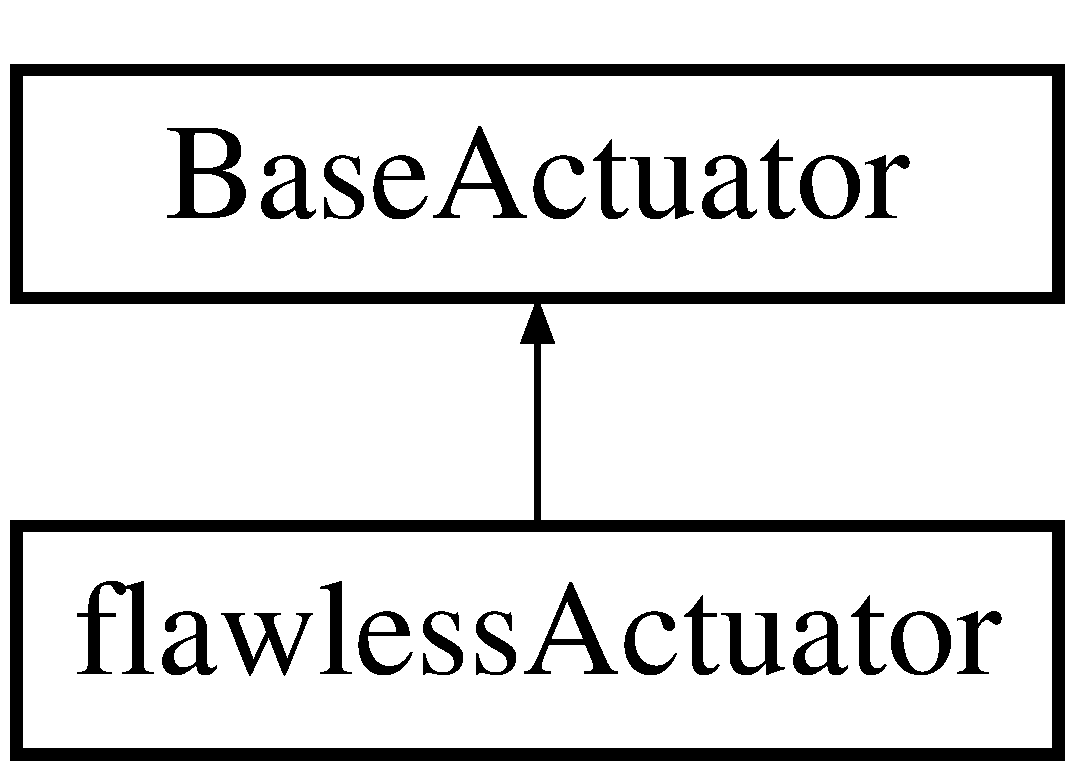
\includegraphics[height=2.000000cm]{class_base_actuator}
\end{center}
\end{figure}
\subsection*{Public Member Functions}
\begin{DoxyCompactItemize}
\item 
\hyperlink{class_base_actuator_a2d0295f149b3db546762ae596d14c6d4}{Base\+Actuator} ()
\begin{DoxyCompactList}\small\item\em construtor \end{DoxyCompactList}\item 
\hyperlink{class_base_actuator_a7326269c65ea05ce4b6aa0333984bf56}{$\sim$\+Base\+Actuator} ()
\begin{DoxyCompactList}\small\item\em construtor \end{DoxyCompactList}\item 
virtual void \hyperlink{class_base_actuator_aa37ef0301610ceba649c25bdaa71fa87}{init\+Actuator} (\hyperlink{group___tools_ga3f1431cb9f76da10f59246d1d743dc2c}{Float64} \&Flight\+Time, Airframe\+Struct \&Airframe\+Data, Actuator\+Struct \&Actuator\+Data)
\begin{DoxyCompactList}\small\item\em initialize selected actuator model \end{DoxyCompactList}\item 
virtual void \hyperlink{class_base_actuator_a8aea3be414ce0dc3afd8e2a54bd523ae}{update\+Actuator} (\hyperlink{group___tools_ga3f1431cb9f76da10f59246d1d743dc2c}{Float64} Flight\+Time, Airframe\+Struct \&Airframe\+Data, Actuator\+Struct \&Actuator\+Data)
\begin{DoxyCompactList}\small\item\em update actuator model \end{DoxyCompactList}\item 
virtual void \hyperlink{class_base_actuator_a60e40bc448e4bea4e079263dd7d78770}{Log\+Actuator\+Data} ()
\begin{DoxyCompactList}\small\item\em log \hyperlink{class_actuator}{Actuator} data \end{DoxyCompactList}\end{DoxyCompactItemize}


\subsection{Detailed Description}
\begin{DoxyAuthor}{Author}
Jan Olucak 
\end{DoxyAuthor}
\begin{DoxyDate}{Date}
25.\+11.\+2017 
\end{DoxyDate}
\begin{DoxyVersion}{Version}
1.\+0
\end{DoxyVersion}
\hyperlink{class_base_actuator}{Base\+Actuator} class is the superclass for all actuator models. Using pointer to base init and update function allows the user to extend the actuators module with new models. 

Definition at line 19 of file Base\+Actuator.\+h.



\subsection{Constructor \& Destructor Documentation}
\mbox{\Hypertarget{class_base_actuator_a2d0295f149b3db546762ae596d14c6d4}\label{class_base_actuator_a2d0295f149b3db546762ae596d14c6d4}} 
\index{Base\+Actuator@{Base\+Actuator}!Base\+Actuator@{Base\+Actuator}}
\index{Base\+Actuator@{Base\+Actuator}!Base\+Actuator@{Base\+Actuator}}
\subsubsection{\texorpdfstring{Base\+Actuator()}{BaseActuator()}}
{\footnotesize\ttfamily Base\+Actuator\+::\+Base\+Actuator (\begin{DoxyParamCaption}{ }\end{DoxyParamCaption})}



construtor 



Definition at line 3 of file Base\+Actuator.\+cpp.

\mbox{\Hypertarget{class_base_actuator_a7326269c65ea05ce4b6aa0333984bf56}\label{class_base_actuator_a7326269c65ea05ce4b6aa0333984bf56}} 
\index{Base\+Actuator@{Base\+Actuator}!````~Base\+Actuator@{$\sim$\+Base\+Actuator}}
\index{````~Base\+Actuator@{$\sim$\+Base\+Actuator}!Base\+Actuator@{Base\+Actuator}}
\subsubsection{\texorpdfstring{$\sim$\+Base\+Actuator()}{~BaseActuator()}}
{\footnotesize\ttfamily Base\+Actuator\+::$\sim$\+Base\+Actuator (\begin{DoxyParamCaption}{ }\end{DoxyParamCaption})}



construtor 



Definition at line 7 of file Base\+Actuator.\+cpp.



\subsection{Member Function Documentation}
\mbox{\Hypertarget{class_base_actuator_aa37ef0301610ceba649c25bdaa71fa87}\label{class_base_actuator_aa37ef0301610ceba649c25bdaa71fa87}} 
\index{Base\+Actuator@{Base\+Actuator}!init\+Actuator@{init\+Actuator}}
\index{init\+Actuator@{init\+Actuator}!Base\+Actuator@{Base\+Actuator}}
\subsubsection{\texorpdfstring{init\+Actuator()}{initActuator()}}
{\footnotesize\ttfamily void Base\+Actuator\+::init\+Actuator (\begin{DoxyParamCaption}\item[{\hyperlink{group___tools_ga3f1431cb9f76da10f59246d1d743dc2c}{Float64} \&}]{Flight\+Time,  }\item[{Airframe\+Struct \&}]{Airframe\+Data,  }\item[{Actuator\+Struct \&}]{Actuator\+Data }\end{DoxyParamCaption})\hspace{0.3cm}{\ttfamily [virtual]}}



initialize selected actuator model 


\begin{DoxyParams}{Parameters}
{\em Flight\+Time} & Flight time \\
\hline
{\em Airframe\+Data} & coammanded actuator angles from autopilot \\
\hline
{\em Actuator\+Data} & real \hyperlink{class_actuator}{Actuator} angles \\
\hline
\end{DoxyParams}


Reimplemented in \hyperlink{classflawless_actuator_a8676b36d0dfd7c8d7d789bdd6135db8f}{flawless\+Actuator}.



Definition at line 11 of file Base\+Actuator.\+cpp.



Referenced by Actuator\+::init\+Actuator().

\mbox{\Hypertarget{class_base_actuator_a60e40bc448e4bea4e079263dd7d78770}\label{class_base_actuator_a60e40bc448e4bea4e079263dd7d78770}} 
\index{Base\+Actuator@{Base\+Actuator}!Log\+Actuator\+Data@{Log\+Actuator\+Data}}
\index{Log\+Actuator\+Data@{Log\+Actuator\+Data}!Base\+Actuator@{Base\+Actuator}}
\subsubsection{\texorpdfstring{Log\+Actuator\+Data()}{LogActuatorData()}}
{\footnotesize\ttfamily void Base\+Actuator\+::\+Log\+Actuator\+Data (\begin{DoxyParamCaption}{ }\end{DoxyParamCaption})\hspace{0.3cm}{\ttfamily [virtual]}}



log \hyperlink{class_actuator}{Actuator} data 



Reimplemented in \hyperlink{classflawless_actuator_a5cd61e149a795ba7db292101d4782bd5}{flawless\+Actuator}.



Definition at line 23 of file Base\+Actuator.\+cpp.



Referenced by Actuator\+::log\+Actuator().

\mbox{\Hypertarget{class_base_actuator_a8aea3be414ce0dc3afd8e2a54bd523ae}\label{class_base_actuator_a8aea3be414ce0dc3afd8e2a54bd523ae}} 
\index{Base\+Actuator@{Base\+Actuator}!update\+Actuator@{update\+Actuator}}
\index{update\+Actuator@{update\+Actuator}!Base\+Actuator@{Base\+Actuator}}
\subsubsection{\texorpdfstring{update\+Actuator()}{updateActuator()}}
{\footnotesize\ttfamily void Base\+Actuator\+::update\+Actuator (\begin{DoxyParamCaption}\item[{\hyperlink{group___tools_ga3f1431cb9f76da10f59246d1d743dc2c}{Float64}}]{Flight\+Time,  }\item[{Airframe\+Struct \&}]{Airframe\+Data,  }\item[{Actuator\+Struct \&}]{Actuator\+Data }\end{DoxyParamCaption})\hspace{0.3cm}{\ttfamily [virtual]}}



update actuator model 


\begin{DoxyParams}{Parameters}
{\em Flight\+Time} & Flight time \\
\hline
{\em Airframe\+Data} & coammanded actuator angles from autopilot \\
\hline
{\em Actuator\+Data} & real \hyperlink{class_actuator}{Actuator} angles \\
\hline
\end{DoxyParams}


Reimplemented in \hyperlink{classflawless_actuator_ad025b033eb040a76cc7d4a7b85ad33da}{flawless\+Actuator}.



Definition at line 17 of file Base\+Actuator.\+cpp.



Referenced by Actuator\+::update\+Actuator().



The documentation for this class was generated from the following files\+:\begin{DoxyCompactItemize}
\item 
C\+:/\+Users/janol/\+Desktop/\+Simulation\+\_\+\+Stand230618/\+Actuator/\hyperlink{_base_actuator_8h}{Base\+Actuator.\+h}\item 
C\+:/\+Users/janol/\+Desktop/\+Simulation\+\_\+\+Stand230618/\+Actuator/\hyperlink{_base_actuator_8cpp}{Base\+Actuator.\+cpp}\end{DoxyCompactItemize}

\hypertarget{class_base_aerodynamic}{}\section{Base\+Aerodynamic Class Reference}
\label{class_base_aerodynamic}\index{Base\+Aerodynamic@{Base\+Aerodynamic}}


{\ttfamily \#include $<$Base\+Aerodynamic.\+h$>$}

Inheritance diagram for Base\+Aerodynamic\+:\begin{figure}[H]
\begin{center}
\leavevmode
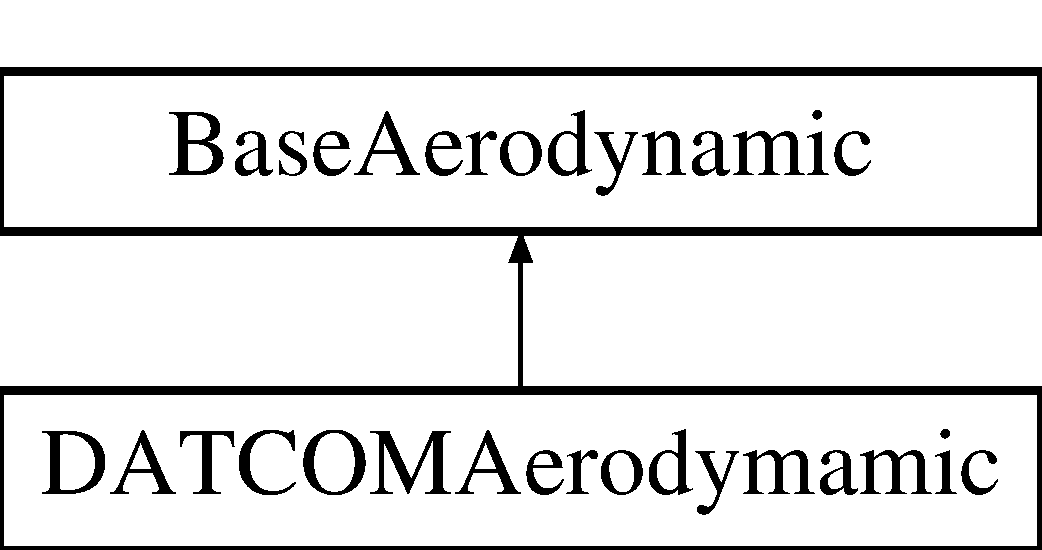
\includegraphics[height=2.000000cm]{class_base_aerodynamic}
\end{center}
\end{figure}
\subsection*{Public Member Functions}
\begin{DoxyCompactItemize}
\item 
\hyperlink{class_base_aerodynamic_aa05d0598119b1364cdb45cf478ae578c}{Base\+Aerodynamic} ()
\begin{DoxyCompactList}\small\item\em constructor \end{DoxyCompactList}\item 
\hyperlink{class_base_aerodynamic_a81d08f3a779e6e25245b6f3b545920cb}{$\sim$\+Base\+Aerodynamic} ()
\begin{DoxyCompactList}\small\item\em destructor \end{DoxyCompactList}\item 
virtual void \hyperlink{class_base_aerodynamic_a6493b7d9c4cbadcbf3a8e5a6c973e1f3}{init\+Aerodynamic} (\hyperlink{group___tools_ga3f1431cb9f76da10f59246d1d743dc2c}{Float64} \&Flight\+Time, Aerodynamic\+Struct \&Aero\+Data, Aircraft\+Struct \&Aircraft\+Data)
\begin{DoxyCompactList}\small\item\em The init function from the selected aerodynamic model is called by a pointer. \end{DoxyCompactList}\item 
virtual void \hyperlink{class_base_aerodynamic_a8a417495c896359b2ee74f5c1c8c08f7}{update\+Aerodynamic} (\hyperlink{group___tools_ga3f1431cb9f76da10f59246d1d743dc2c}{Float64} Flight\+Time, Atmosphere\+Struct \&Atmo\+Data, Aerodynamic\+Struct \&Aero\+Data, Airframe\+Struct \&Airframe\+Data, Thrust\+Struct \&Thrust\+Data, Actuator\+Struct \&Actuator\+Data, I\+M\+U\+Struct \&I\+M\+U\+Data, Navigation\+Struct \&Nav\+Data)
\begin{DoxyCompactList}\small\item\em calculate aero forces and moments \end{DoxyCompactList}\item 
virtual void \hyperlink{class_base_aerodynamic_abaea76739e197627a6d09cff5b68af83}{Log\+Aero\+Data} ()
\begin{DoxyCompactList}\small\item\em log aerodynamic data to text file \end{DoxyCompactList}\end{DoxyCompactItemize}


\subsection{Detailed Description}
\begin{DoxyAuthor}{Author}
Jan Olucak 
\end{DoxyAuthor}
\begin{DoxyDate}{Date}
25.\+11.\+2017 
\end{DoxyDate}
\begin{DoxyVersion}{Version}
1.\+0
\end{DoxyVersion}
Base Aerodynamic class is the superclass for all aerodynamic models. Using pointer to base init and update function allows the user to extend the aerodynamic module with new models. 

Definition at line 21 of file Base\+Aerodynamic.\+h.



\subsection{Constructor \& Destructor Documentation}
\mbox{\Hypertarget{class_base_aerodynamic_aa05d0598119b1364cdb45cf478ae578c}\label{class_base_aerodynamic_aa05d0598119b1364cdb45cf478ae578c}} 
\index{Base\+Aerodynamic@{Base\+Aerodynamic}!Base\+Aerodynamic@{Base\+Aerodynamic}}
\index{Base\+Aerodynamic@{Base\+Aerodynamic}!Base\+Aerodynamic@{Base\+Aerodynamic}}
\subsubsection{\texorpdfstring{Base\+Aerodynamic()}{BaseAerodynamic()}}
{\footnotesize\ttfamily Base\+Aerodynamic\+::\+Base\+Aerodynamic (\begin{DoxyParamCaption}{ }\end{DoxyParamCaption})}



constructor 



Definition at line 3 of file Base\+Aerodynamic.\+cpp.

\mbox{\Hypertarget{class_base_aerodynamic_a81d08f3a779e6e25245b6f3b545920cb}\label{class_base_aerodynamic_a81d08f3a779e6e25245b6f3b545920cb}} 
\index{Base\+Aerodynamic@{Base\+Aerodynamic}!````~Base\+Aerodynamic@{$\sim$\+Base\+Aerodynamic}}
\index{````~Base\+Aerodynamic@{$\sim$\+Base\+Aerodynamic}!Base\+Aerodynamic@{Base\+Aerodynamic}}
\subsubsection{\texorpdfstring{$\sim$\+Base\+Aerodynamic()}{~BaseAerodynamic()}}
{\footnotesize\ttfamily Base\+Aerodynamic\+::$\sim$\+Base\+Aerodynamic (\begin{DoxyParamCaption}{ }\end{DoxyParamCaption})}



destructor 



Definition at line 7 of file Base\+Aerodynamic.\+cpp.



\subsection{Member Function Documentation}
\mbox{\Hypertarget{class_base_aerodynamic_a6493b7d9c4cbadcbf3a8e5a6c973e1f3}\label{class_base_aerodynamic_a6493b7d9c4cbadcbf3a8e5a6c973e1f3}} 
\index{Base\+Aerodynamic@{Base\+Aerodynamic}!init\+Aerodynamic@{init\+Aerodynamic}}
\index{init\+Aerodynamic@{init\+Aerodynamic}!Base\+Aerodynamic@{Base\+Aerodynamic}}
\subsubsection{\texorpdfstring{init\+Aerodynamic()}{initAerodynamic()}}
{\footnotesize\ttfamily void Base\+Aerodynamic\+::init\+Aerodynamic (\begin{DoxyParamCaption}\item[{\hyperlink{group___tools_ga3f1431cb9f76da10f59246d1d743dc2c}{Float64} \&}]{Flight\+Time,  }\item[{Aerodynamic\+Struct \&}]{Aero\+Data,  }\item[{Aircraft\+Struct \&}]{Aircraft\+Data }\end{DoxyParamCaption})\hspace{0.3cm}{\ttfamily [virtual]}}



The init function from the selected aerodynamic model is called by a pointer. 


\begin{DoxyParams}{Parameters}
{\em Flight\+Time} & flighttime \\
\hline
{\em Aero\+Data} & structure of aero data \\
\hline
{\em Aircraft\+Data} & structure of aircraft data \\
\hline
\end{DoxyParams}


Reimplemented in \hyperlink{class_d_a_t_c_o_m_aerodymamic_aa4909fb5e6db41f2309b7d8a8658a219}{D\+A\+T\+C\+O\+M\+Aerodymamic}.



Definition at line 25 of file Base\+Aerodynamic.\+cpp.



Referenced by Aerodynamics\+::init\+Aerodynamic().

\mbox{\Hypertarget{class_base_aerodynamic_abaea76739e197627a6d09cff5b68af83}\label{class_base_aerodynamic_abaea76739e197627a6d09cff5b68af83}} 
\index{Base\+Aerodynamic@{Base\+Aerodynamic}!Log\+Aero\+Data@{Log\+Aero\+Data}}
\index{Log\+Aero\+Data@{Log\+Aero\+Data}!Base\+Aerodynamic@{Base\+Aerodynamic}}
\subsubsection{\texorpdfstring{Log\+Aero\+Data()}{LogAeroData()}}
{\footnotesize\ttfamily void Base\+Aerodynamic\+::\+Log\+Aero\+Data (\begin{DoxyParamCaption}{ }\end{DoxyParamCaption})\hspace{0.3cm}{\ttfamily [virtual]}}



log aerodynamic data to text file 



Reimplemented in \hyperlink{class_d_a_t_c_o_m_aerodymamic_a84ab90acbbec700e0b06272bf95cf932}{D\+A\+T\+C\+O\+M\+Aerodymamic}.



Definition at line 32 of file Base\+Aerodynamic.\+cpp.



Referenced by Aerodynamics\+::\+Log\+Aero\+Data().

\mbox{\Hypertarget{class_base_aerodynamic_a8a417495c896359b2ee74f5c1c8c08f7}\label{class_base_aerodynamic_a8a417495c896359b2ee74f5c1c8c08f7}} 
\index{Base\+Aerodynamic@{Base\+Aerodynamic}!update\+Aerodynamic@{update\+Aerodynamic}}
\index{update\+Aerodynamic@{update\+Aerodynamic}!Base\+Aerodynamic@{Base\+Aerodynamic}}
\subsubsection{\texorpdfstring{update\+Aerodynamic()}{updateAerodynamic()}}
{\footnotesize\ttfamily void Base\+Aerodynamic\+::update\+Aerodynamic (\begin{DoxyParamCaption}\item[{\hyperlink{group___tools_ga3f1431cb9f76da10f59246d1d743dc2c}{Float64}}]{Flight\+Time,  }\item[{Atmosphere\+Struct \&}]{Atmo\+Data,  }\item[{Aerodynamic\+Struct \&}]{Aero\+Data,  }\item[{Airframe\+Struct \&}]{Airframe\+Data,  }\item[{Thrust\+Struct \&}]{Thrust\+Data,  }\item[{Actuator\+Struct \&}]{Actuator\+Data,  }\item[{I\+M\+U\+Struct \&}]{I\+M\+U\+Data,  }\item[{Navigation\+Struct \&}]{Nav\+Data }\end{DoxyParamCaption})\hspace{0.3cm}{\ttfamily [virtual]}}



calculate aero forces and moments 


\begin{DoxyParams}{Parameters}
{\em Flight\+Time} & Flight Time \\
\hline
{\em Atmo\+Data} & air density, speed of sound \\
\hline
{\em Aero\+Data} & structure of aero data \\
\hline
{\em Airframe\+Data} & structure of airframe data \\
\hline
{\em Thrust\+Data} & structure of thrust data \\
\hline
{\em Actuator\+Data} & actuator angles \\
\hline
{\em I\+M\+U\+Data} & rotational rates \\
\hline
{\em Nav\+Data} & \hyperlink{class_navigation}{Navigation} data like velocity in N\+ED system \\
\hline
\end{DoxyParams}


Reimplemented in \hyperlink{class_d_a_t_c_o_m_aerodymamic_a501386a4e5d176d3fb8bddae1d0c8d0f}{D\+A\+T\+C\+O\+M\+Aerodymamic}.



Definition at line 11 of file Base\+Aerodynamic.\+cpp.



Referenced by Aerodynamics\+::update\+Aerodynamic().



The documentation for this class was generated from the following files\+:\begin{DoxyCompactItemize}
\item 
C\+:/\+Users/janol/\+Desktop/\+Simulation\+\_\+\+Stand230618/\+Aerodynamic/\hyperlink{_base_aerodynamic_8h}{Base\+Aerodynamic.\+h}\item 
C\+:/\+Users/janol/\+Desktop/\+Simulation\+\_\+\+Stand230618/\+Aerodynamic/\hyperlink{_base_aerodynamic_8cpp}{Base\+Aerodynamic.\+cpp}\end{DoxyCompactItemize}

\hypertarget{class_base_g_p_s}{}\section{Base\+G\+PS Class Reference}
\label{class_base_g_p_s}\index{Base\+G\+PS@{Base\+G\+PS}}


{\ttfamily \#include $<$Base\+G\+P\+S.\+h$>$}

Inheritance diagram for Base\+G\+PS\+:\begin{figure}[H]
\begin{center}
\leavevmode
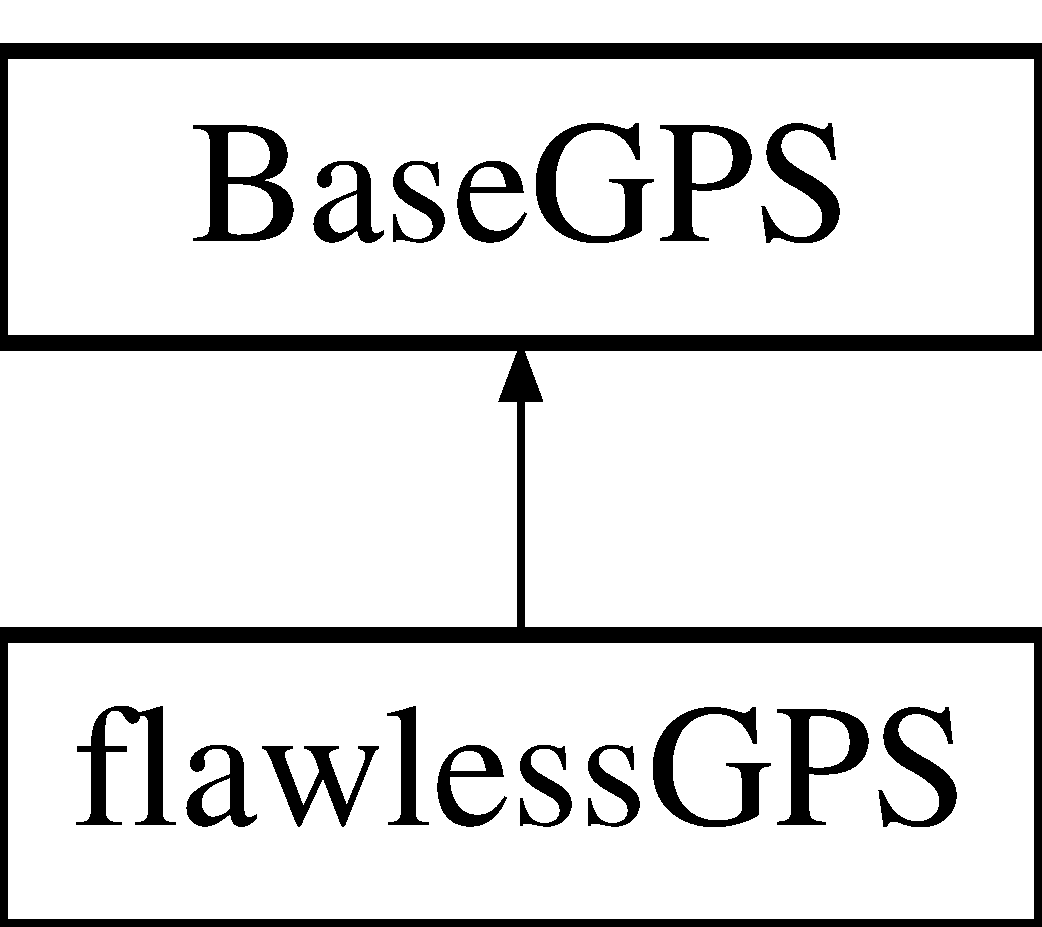
\includegraphics[height=2.000000cm]{class_base_g_p_s}
\end{center}
\end{figure}
\subsection*{Public Member Functions}
\begin{DoxyCompactItemize}
\item 
\hyperlink{class_base_g_p_s_a224584d4b12f0663d9fb2caf996d05bb}{Base\+G\+PS} ()
\begin{DoxyCompactList}\small\item\em constructor \end{DoxyCompactList}\item 
\hyperlink{class_base_g_p_s_aa80ae9016c4e52d7654435b122106434}{$\sim$\+Base\+G\+PS} ()
\begin{DoxyCompactList}\small\item\em destructor \end{DoxyCompactList}\item 
virtual void \hyperlink{class_base_g_p_s_a68dbbdd67e5d9de606810377f1cec0e3}{init\+G\+PS} ()
\begin{DoxyCompactList}\small\item\em initialize \hyperlink{class_g_p_s}{G\+PS} \end{DoxyCompactList}\item 
virtual void \hyperlink{class_base_g_p_s_ac8bb7ab0f8b35a5e6a29fed125268ce6}{update\+G\+PS} (\hyperlink{group___tools_ga3f1431cb9f76da10f59246d1d743dc2c}{Float64} Flight\+Time, Navigation\+Struct \&Nav\+Data, Airframe\+Struct \&Airframe\+Data)
\begin{DoxyCompactList}\small\item\em update \hyperlink{class_g_p_s}{G\+PS} data \end{DoxyCompactList}\item 
virtual void \hyperlink{class_base_g_p_s_ad62094ad9ac6e9813cd65e63aeb7df13}{log\+G\+P\+S\+Data} ()
\begin{DoxyCompactList}\small\item\em log \hyperlink{class_g_p_s}{G\+PS} data \end{DoxyCompactList}\end{DoxyCompactItemize}


\subsection{Detailed Description}
\begin{DoxyAuthor}{Author}
Jan Olucak 
\end{DoxyAuthor}
\begin{DoxyDate}{Date}
02.\+01.\+2018 
\end{DoxyDate}
\begin{DoxyVersion}{Version}
1.\+0
\end{DoxyVersion}
\hyperlink{class_base_g_p_s}{Base\+G\+PS} class is the superclass for all \hyperlink{class_g_p_s}{G\+PS} models. Using pointer to base init and update function allows the user to extend the \hyperlink{class_g_p_s}{G\+PS} module with new models. 

Definition at line 21 of file Base\+G\+P\+S.\+h.



\subsection{Constructor \& Destructor Documentation}
\mbox{\Hypertarget{class_base_g_p_s_a224584d4b12f0663d9fb2caf996d05bb}\label{class_base_g_p_s_a224584d4b12f0663d9fb2caf996d05bb}} 
\index{Base\+G\+PS@{Base\+G\+PS}!Base\+G\+PS@{Base\+G\+PS}}
\index{Base\+G\+PS@{Base\+G\+PS}!Base\+G\+PS@{Base\+G\+PS}}
\subsubsection{\texorpdfstring{Base\+G\+P\+S()}{BaseGPS()}}
{\footnotesize\ttfamily Base\+G\+P\+S\+::\+Base\+G\+PS (\begin{DoxyParamCaption}{ }\end{DoxyParamCaption})}



constructor 



Definition at line 3 of file Base\+G\+P\+S.\+cpp.

\mbox{\Hypertarget{class_base_g_p_s_aa80ae9016c4e52d7654435b122106434}\label{class_base_g_p_s_aa80ae9016c4e52d7654435b122106434}} 
\index{Base\+G\+PS@{Base\+G\+PS}!````~Base\+G\+PS@{$\sim$\+Base\+G\+PS}}
\index{````~Base\+G\+PS@{$\sim$\+Base\+G\+PS}!Base\+G\+PS@{Base\+G\+PS}}
\subsubsection{\texorpdfstring{$\sim$\+Base\+G\+P\+S()}{~BaseGPS()}}
{\footnotesize\ttfamily Base\+G\+P\+S\+::$\sim$\+Base\+G\+PS (\begin{DoxyParamCaption}{ }\end{DoxyParamCaption})}



destructor 



Definition at line 7 of file Base\+G\+P\+S.\+cpp.



\subsection{Member Function Documentation}
\mbox{\Hypertarget{class_base_g_p_s_a68dbbdd67e5d9de606810377f1cec0e3}\label{class_base_g_p_s_a68dbbdd67e5d9de606810377f1cec0e3}} 
\index{Base\+G\+PS@{Base\+G\+PS}!init\+G\+PS@{init\+G\+PS}}
\index{init\+G\+PS@{init\+G\+PS}!Base\+G\+PS@{Base\+G\+PS}}
\subsubsection{\texorpdfstring{init\+G\+P\+S()}{initGPS()}}
{\footnotesize\ttfamily void Base\+G\+P\+S\+::init\+G\+PS (\begin{DoxyParamCaption}{ }\end{DoxyParamCaption})\hspace{0.3cm}{\ttfamily [virtual]}}



initialize \hyperlink{class_g_p_s}{G\+PS} 



Reimplemented in \hyperlink{classflawless_g_p_s_a50cdffc0dc65e644f6191bc7c723521b}{flawless\+G\+PS}.



Definition at line 11 of file Base\+G\+P\+S.\+cpp.



Referenced by G\+P\+S\+::init\+G\+P\+S().

\mbox{\Hypertarget{class_base_g_p_s_ad62094ad9ac6e9813cd65e63aeb7df13}\label{class_base_g_p_s_ad62094ad9ac6e9813cd65e63aeb7df13}} 
\index{Base\+G\+PS@{Base\+G\+PS}!log\+G\+P\+S\+Data@{log\+G\+P\+S\+Data}}
\index{log\+G\+P\+S\+Data@{log\+G\+P\+S\+Data}!Base\+G\+PS@{Base\+G\+PS}}
\subsubsection{\texorpdfstring{log\+G\+P\+S\+Data()}{logGPSData()}}
{\footnotesize\ttfamily void Base\+G\+P\+S\+::log\+G\+P\+S\+Data (\begin{DoxyParamCaption}{ }\end{DoxyParamCaption})\hspace{0.3cm}{\ttfamily [virtual]}}



log \hyperlink{class_g_p_s}{G\+PS} data 



Reimplemented in \hyperlink{classflawless_g_p_s_a764a28d4434bd497b3701dbff915291f}{flawless\+G\+PS}.



Definition at line 24 of file Base\+G\+P\+S.\+cpp.

\mbox{\Hypertarget{class_base_g_p_s_ac8bb7ab0f8b35a5e6a29fed125268ce6}\label{class_base_g_p_s_ac8bb7ab0f8b35a5e6a29fed125268ce6}} 
\index{Base\+G\+PS@{Base\+G\+PS}!update\+G\+PS@{update\+G\+PS}}
\index{update\+G\+PS@{update\+G\+PS}!Base\+G\+PS@{Base\+G\+PS}}
\subsubsection{\texorpdfstring{update\+G\+P\+S()}{updateGPS()}}
{\footnotesize\ttfamily void Base\+G\+P\+S\+::update\+G\+PS (\begin{DoxyParamCaption}\item[{\hyperlink{group___tools_ga3f1431cb9f76da10f59246d1d743dc2c}{Float64}}]{Flight\+Time,  }\item[{Navigation\+Struct \&}]{Nav\+Data,  }\item[{Airframe\+Struct \&}]{Airframe\+Data }\end{DoxyParamCaption})\hspace{0.3cm}{\ttfamily [virtual]}}



update \hyperlink{class_g_p_s}{G\+PS} data 


\begin{DoxyParams}{Parameters}
{\em Flight\+Time} & flighttime \\
\hline
{\em Nav\+Data} & structure of navigation data \\
\hline
{\em Airframe\+Data} & flight states \\
\hline
\end{DoxyParams}


Reimplemented in \hyperlink{classflawless_g_p_s_aa93a0161307e087120572c717dd42a70}{flawless\+G\+PS}.



Definition at line 17 of file Base\+G\+P\+S.\+cpp.



Referenced by G\+P\+S\+::update\+G\+P\+S().



The documentation for this class was generated from the following files\+:\begin{DoxyCompactItemize}
\item 
C\+:/\+Users/janol/\+Desktop/\+Simulation\+\_\+\+Stand230618/\+G\+P\+S/\hyperlink{_base_g_p_s_8h}{Base\+G\+P\+S.\+h}\item 
C\+:/\+Users/janol/\+Desktop/\+Simulation\+\_\+\+Stand230618/\+G\+P\+S/\hyperlink{_base_g_p_s_8cpp}{Base\+G\+P\+S.\+cpp}\end{DoxyCompactItemize}

\hypertarget{class_base_guidance}{}\section{Base\+Guidance Class Reference}
\label{class_base_guidance}\index{Base\+Guidance@{Base\+Guidance}}


{\ttfamily \#include $<$Base\+Guidance.\+h$>$}

Inheritance diagram for Base\+Guidance\+:\begin{figure}[H]
\begin{center}
\leavevmode
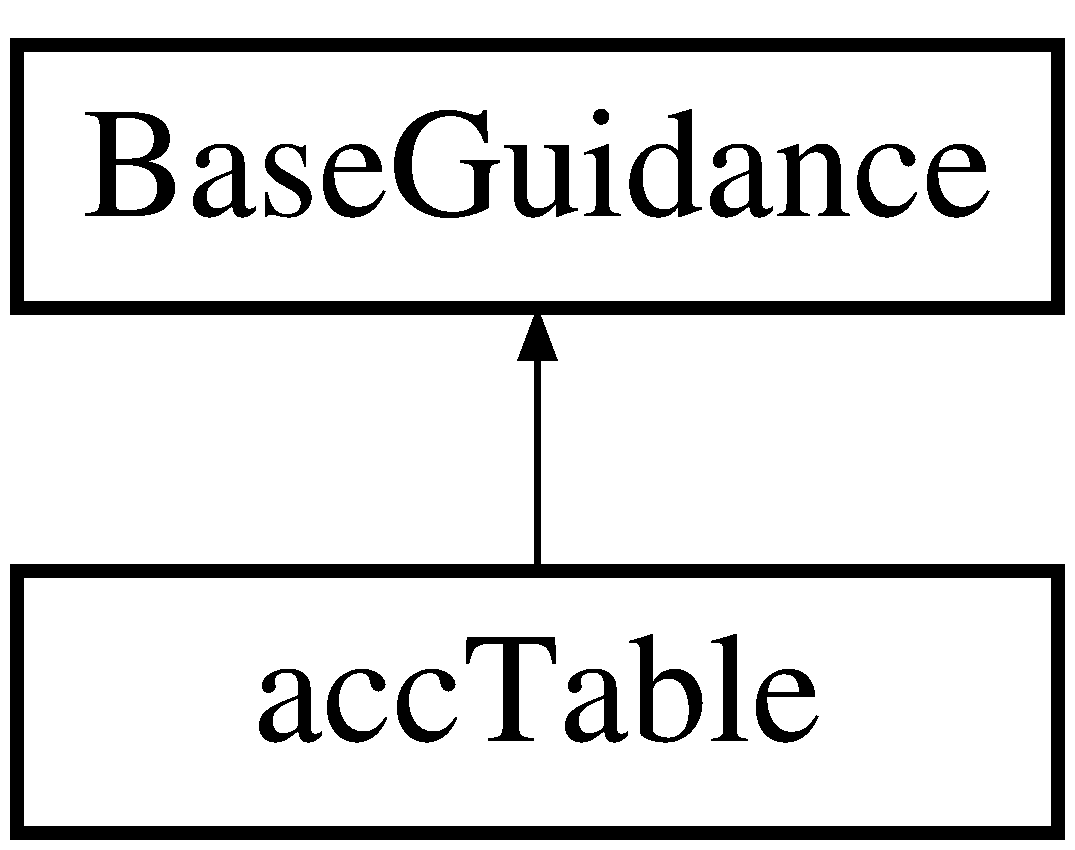
\includegraphics[height=2.000000cm]{class_base_guidance}
\end{center}
\end{figure}
\subsection*{Public Member Functions}
\begin{DoxyCompactItemize}
\item 
\hyperlink{class_base_guidance_aa96d54da1d306fcfbf05705eabc91c55}{Base\+Guidance} ()
\begin{DoxyCompactList}\small\item\em constructor \end{DoxyCompactList}\item 
\hyperlink{class_base_guidance_a28666e14c8ecedcfb33191ee273316c6}{$\sim$\+Base\+Guidance} ()
\begin{DoxyCompactList}\small\item\em destructor \end{DoxyCompactList}\item 
virtual void \hyperlink{class_base_guidance_a8eacaa605a7691b5cc23870e98615551}{init\+Guidance} (\hyperlink{group___tools_ga3f1431cb9f76da10f59246d1d743dc2c}{Float64} \&Flight\+Time, Guidance\+Struct \&Guidance\+Data, Aircraft\+Struct \&Aircraft\+Data)
\begin{DoxyCompactList}\small\item\em acc\+Tables are read in and stored in row vectors \end{DoxyCompactList}\item 
virtual void \hyperlink{class_base_guidance_a0092008303b3fcc7664d04892c4878c3}{update\+Guidance} (\hyperlink{group___tools_ga3f1431cb9f76da10f59246d1d743dc2c}{Float64} Flight\+Time, Aerodynamic\+Struct \&Aero\+Data, Thrust\+Struct \&Thrust\+Data, Airframe\+Struct \&Airframe\+Data, Guidance\+Struct \&Guidance\+Data)
\begin{DoxyCompactList}\small\item\em calculate commands for flight path \end{DoxyCompactList}\item 
virtual void \hyperlink{class_base_guidance_ac1c54d52fe315199e45061060602be0f}{init\+Log\+Guidance} (\hyperlink{group___tools_ga3f1431cb9f76da10f59246d1d743dc2c}{Float64} Flight\+Time, Guidance\+Struct \&Guidance\+Data)
\begin{DoxyCompactList}\small\item\em define output for guidance data \end{DoxyCompactList}\item 
virtual void \hyperlink{class_base_guidance_af3bd60f6f17739864fbfa3ec2467ae04}{log\+Guidance\+Data} ()
\begin{DoxyCompactList}\small\item\em log guidance data \end{DoxyCompactList}\end{DoxyCompactItemize}


\subsection{Detailed Description}
\begin{DoxyAuthor}{Author}
Jan Olucak 
\end{DoxyAuthor}
\begin{DoxyDate}{Date}
23.\+12.\+2017 
\end{DoxyDate}
\begin{DoxyVersion}{Version}
1.\+0
\end{DoxyVersion}
\hyperlink{class_base_guidance}{Base\+Guidance} is the superclass for all guidance models 

Definition at line 18 of file Base\+Guidance.\+h.



\subsection{Constructor \& Destructor Documentation}
\mbox{\Hypertarget{class_base_guidance_aa96d54da1d306fcfbf05705eabc91c55}\label{class_base_guidance_aa96d54da1d306fcfbf05705eabc91c55}} 
\index{Base\+Guidance@{Base\+Guidance}!Base\+Guidance@{Base\+Guidance}}
\index{Base\+Guidance@{Base\+Guidance}!Base\+Guidance@{Base\+Guidance}}
\subsubsection{\texorpdfstring{Base\+Guidance()}{BaseGuidance()}}
{\footnotesize\ttfamily Base\+Guidance\+::\+Base\+Guidance (\begin{DoxyParamCaption}{ }\end{DoxyParamCaption})}



constructor 



Definition at line 3 of file Base\+Guidance.\+cpp.

\mbox{\Hypertarget{class_base_guidance_a28666e14c8ecedcfb33191ee273316c6}\label{class_base_guidance_a28666e14c8ecedcfb33191ee273316c6}} 
\index{Base\+Guidance@{Base\+Guidance}!````~Base\+Guidance@{$\sim$\+Base\+Guidance}}
\index{````~Base\+Guidance@{$\sim$\+Base\+Guidance}!Base\+Guidance@{Base\+Guidance}}
\subsubsection{\texorpdfstring{$\sim$\+Base\+Guidance()}{~BaseGuidance()}}
{\footnotesize\ttfamily Base\+Guidance\+::$\sim$\+Base\+Guidance (\begin{DoxyParamCaption}{ }\end{DoxyParamCaption})}



destructor 



Definition at line 7 of file Base\+Guidance.\+cpp.



\subsection{Member Function Documentation}
\mbox{\Hypertarget{class_base_guidance_a8eacaa605a7691b5cc23870e98615551}\label{class_base_guidance_a8eacaa605a7691b5cc23870e98615551}} 
\index{Base\+Guidance@{Base\+Guidance}!init\+Guidance@{init\+Guidance}}
\index{init\+Guidance@{init\+Guidance}!Base\+Guidance@{Base\+Guidance}}
\subsubsection{\texorpdfstring{init\+Guidance()}{initGuidance()}}
{\footnotesize\ttfamily void Base\+Guidance\+::init\+Guidance (\begin{DoxyParamCaption}\item[{\hyperlink{group___tools_ga3f1431cb9f76da10f59246d1d743dc2c}{Float64} \&}]{Flight\+Time,  }\item[{Guidance\+Struct \&}]{Guidance\+Data,  }\item[{Aircraft\+Struct \&}]{Aircraft\+Data }\end{DoxyParamCaption})\hspace{0.3cm}{\ttfamily [virtual]}}



acc\+Tables are read in and stored in row vectors 


\begin{DoxyParams}{Parameters}
{\em Flight\+Time} & flight time \\
\hline
{\em Guidance\+Data} & structure of \hyperlink{class_guidance}{Guidance} data \\
\hline
{\em Aircraft\+Data} & specific airfraft data \\
\hline
\end{DoxyParams}


Reimplemented in \hyperlink{classacc_table_ad477c8d63acae0be3f974b1a90b43e58}{acc\+Table}.



Definition at line 11 of file Base\+Guidance.\+cpp.



Referenced by Guidance\+::init\+Guidance().

\mbox{\Hypertarget{class_base_guidance_ac1c54d52fe315199e45061060602be0f}\label{class_base_guidance_ac1c54d52fe315199e45061060602be0f}} 
\index{Base\+Guidance@{Base\+Guidance}!init\+Log\+Guidance@{init\+Log\+Guidance}}
\index{init\+Log\+Guidance@{init\+Log\+Guidance}!Base\+Guidance@{Base\+Guidance}}
\subsubsection{\texorpdfstring{init\+Log\+Guidance()}{initLogGuidance()}}
{\footnotesize\ttfamily void Base\+Guidance\+::init\+Log\+Guidance (\begin{DoxyParamCaption}\item[{\hyperlink{group___tools_ga3f1431cb9f76da10f59246d1d743dc2c}{Float64}}]{Flight\+Time,  }\item[{Guidance\+Struct \&}]{Guidance\+Data }\end{DoxyParamCaption})\hspace{0.3cm}{\ttfamily [virtual]}}



define output for guidance data 


\begin{DoxyParams}{Parameters}
{\em Flight\+Time} & flight time \\
\hline
{\em Guidance\+Data} & structure of guidance data \\
\hline
\end{DoxyParams}


Definition at line 25 of file Base\+Guidance.\+cpp.

\mbox{\Hypertarget{class_base_guidance_af3bd60f6f17739864fbfa3ec2467ae04}\label{class_base_guidance_af3bd60f6f17739864fbfa3ec2467ae04}} 
\index{Base\+Guidance@{Base\+Guidance}!log\+Guidance\+Data@{log\+Guidance\+Data}}
\index{log\+Guidance\+Data@{log\+Guidance\+Data}!Base\+Guidance@{Base\+Guidance}}
\subsubsection{\texorpdfstring{log\+Guidance\+Data()}{logGuidanceData()}}
{\footnotesize\ttfamily void Base\+Guidance\+::log\+Guidance\+Data (\begin{DoxyParamCaption}{ }\end{DoxyParamCaption})\hspace{0.3cm}{\ttfamily [virtual]}}



log guidance data 



Reimplemented in \hyperlink{classacc_table_ace4665dcb6e791bbd30ba0f0abb79461}{acc\+Table}.



Definition at line 30 of file Base\+Guidance.\+cpp.



Referenced by Guidance\+::log\+Guidance\+Data().

\mbox{\Hypertarget{class_base_guidance_a0092008303b3fcc7664d04892c4878c3}\label{class_base_guidance_a0092008303b3fcc7664d04892c4878c3}} 
\index{Base\+Guidance@{Base\+Guidance}!update\+Guidance@{update\+Guidance}}
\index{update\+Guidance@{update\+Guidance}!Base\+Guidance@{Base\+Guidance}}
\subsubsection{\texorpdfstring{update\+Guidance()}{updateGuidance()}}
{\footnotesize\ttfamily void Base\+Guidance\+::update\+Guidance (\begin{DoxyParamCaption}\item[{\hyperlink{group___tools_ga3f1431cb9f76da10f59246d1d743dc2c}{Float64}}]{Flight\+Time,  }\item[{Aerodynamic\+Struct \&}]{Aero\+Data,  }\item[{Thrust\+Struct \&}]{Thrust\+Data,  }\item[{Airframe\+Struct \&}]{Airframe\+Data,  }\item[{Guidance\+Struct \&}]{Guidance\+Data }\end{DoxyParamCaption})\hspace{0.3cm}{\ttfamily [virtual]}}



calculate commands for flight path 


\begin{DoxyParams}{Parameters}
{\em Flight\+Time} & flight time \\
\hline
{\em Aero\+Data} & structure of aero data \\
\hline
{\em Thrust\+Data} & structure of thrust data \\
\hline
{\em Airframe\+Data} & structure of airframe data \\
\hline
{\em Guidance\+Data} & structure of guidance data \\
\hline
\end{DoxyParams}


Reimplemented in \hyperlink{classacc_table_a60a9fdb7b041cd5aae020c4a5d252fba}{acc\+Table}.



Definition at line 16 of file Base\+Guidance.\+cpp.



Referenced by Guidance\+::update\+Guidance().



The documentation for this class was generated from the following files\+:\begin{DoxyCompactItemize}
\item 
C\+:/\+Users/janol/\+Desktop/\+Simulation\+\_\+\+Stand230618/\+Guidance/\hyperlink{_base_guidance_8h}{Base\+Guidance.\+h}\item 
C\+:/\+Users/janol/\+Desktop/\+Simulation\+\_\+\+Stand230618/\+Guidance/\hyperlink{_base_guidance_8cpp}{Base\+Guidance.\+cpp}\end{DoxyCompactItemize}

\hypertarget{class_base_i_m_u}{}\section{Base\+I\+MU Class Reference}
\label{class_base_i_m_u}\index{Base\+I\+MU@{Base\+I\+MU}}


{\ttfamily \#include $<$Base\+I\+M\+U.\+h$>$}

Inheritance diagram for Base\+I\+MU\+:\begin{figure}[H]
\begin{center}
\leavevmode
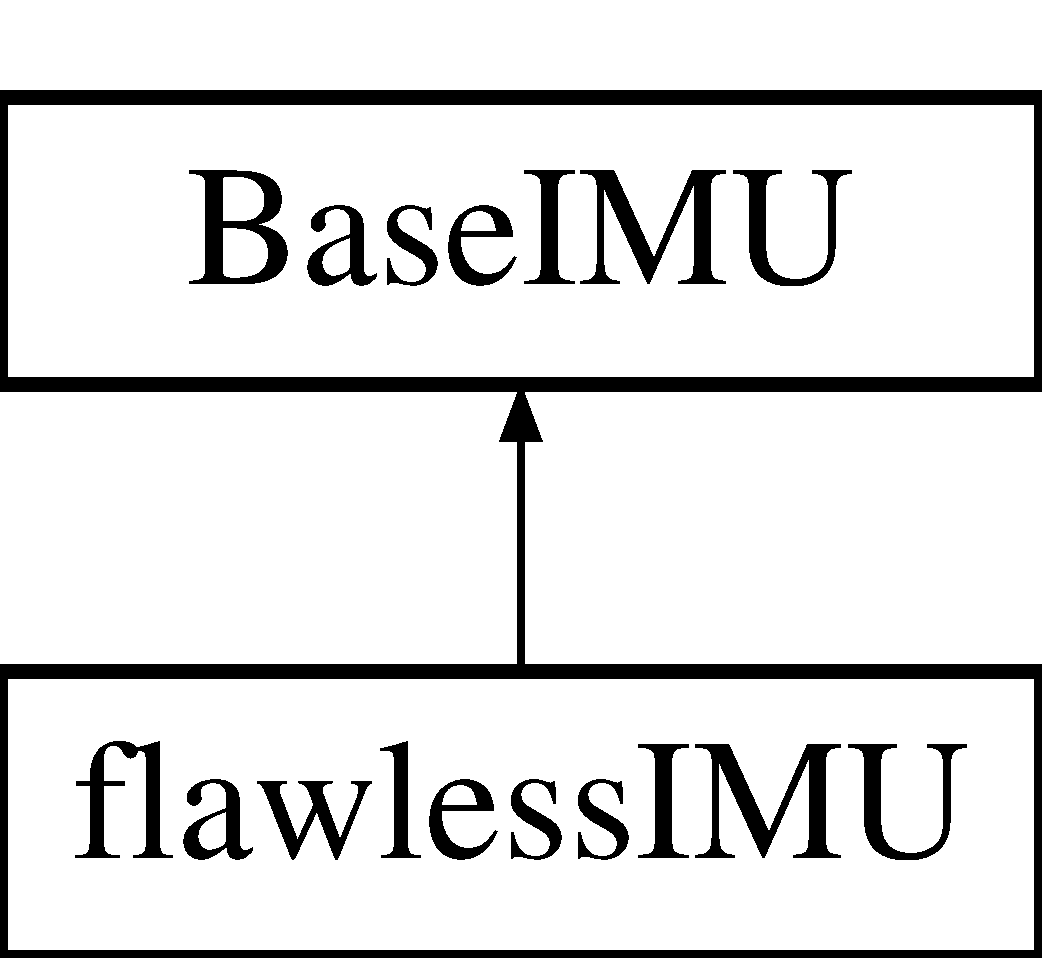
\includegraphics[height=2.000000cm]{class_base_i_m_u}
\end{center}
\end{figure}
\subsection*{Public Member Functions}
\begin{DoxyCompactItemize}
\item 
\hyperlink{class_base_i_m_u_a83201acc90b4dad87a64f0196ec9e282}{Base\+I\+MU} ()
\begin{DoxyCompactList}\small\item\em constructor \end{DoxyCompactList}\item 
\hyperlink{class_base_i_m_u_ae986c3e646b24fc8d58faf6ae72e3841}{$\sim$\+Base\+I\+MU} ()
\begin{DoxyCompactList}\small\item\em destructor \end{DoxyCompactList}\item 
virtual void \hyperlink{class_base_i_m_u_ade02045afd03f290ac1e702db9e1d5a7}{init\+I\+MU} (I\+M\+U\+Struct \&I\+M\+U\+Data)
\begin{DoxyCompactList}\small\item\em initialize \hyperlink{class_i_m_u}{I\+MU} \end{DoxyCompactList}\item 
virtual void \hyperlink{class_base_i_m_u_abd0f60caf589832c53e185c80ce89f3c}{update\+I\+MU} (\hyperlink{group___tools_ga3f1431cb9f76da10f59246d1d743dc2c}{Float64} Flight\+Time, Airframe\+Struct \&Airframe\+Data, I\+M\+U\+Struct \&I\+M\+U\+Data)
\begin{DoxyCompactList}\small\item\em update \hyperlink{class_i_m_u}{I\+MU} \end{DoxyCompactList}\item 
virtual void \hyperlink{class_base_i_m_u_a8f323eb821f92300af5047ed9c66b116}{log\+I\+M\+U\+Data} ()
\begin{DoxyCompactList}\small\item\em log \hyperlink{class_i_m_u}{I\+MU} data \end{DoxyCompactList}\end{DoxyCompactItemize}


\subsection{Detailed Description}
\begin{DoxyAuthor}{Author}
Jan Olucak 
\end{DoxyAuthor}
\begin{DoxyDate}{Date}
02.\+01.\+2018 
\end{DoxyDate}
\begin{DoxyVersion}{Version}
1.\+0
\end{DoxyVersion}
\hyperlink{class_base_i_m_u}{Base\+I\+MU} class is the superclass for all \hyperlink{class_g_p_s}{G\+PS} models. Using pointer to base init and update function allows the user to extend the \hyperlink{class_i_m_u}{I\+MU} module with new models. 

Definition at line 18 of file Base\+I\+M\+U.\+h.



\subsection{Constructor \& Destructor Documentation}
\mbox{\Hypertarget{class_base_i_m_u_a83201acc90b4dad87a64f0196ec9e282}\label{class_base_i_m_u_a83201acc90b4dad87a64f0196ec9e282}} 
\index{Base\+I\+MU@{Base\+I\+MU}!Base\+I\+MU@{Base\+I\+MU}}
\index{Base\+I\+MU@{Base\+I\+MU}!Base\+I\+MU@{Base\+I\+MU}}
\subsubsection{\texorpdfstring{Base\+I\+M\+U()}{BaseIMU()}}
{\footnotesize\ttfamily Base\+I\+M\+U\+::\+Base\+I\+MU (\begin{DoxyParamCaption}{ }\end{DoxyParamCaption})}



constructor 



Definition at line 3 of file Base\+I\+M\+U.\+cpp.

\mbox{\Hypertarget{class_base_i_m_u_ae986c3e646b24fc8d58faf6ae72e3841}\label{class_base_i_m_u_ae986c3e646b24fc8d58faf6ae72e3841}} 
\index{Base\+I\+MU@{Base\+I\+MU}!````~Base\+I\+MU@{$\sim$\+Base\+I\+MU}}
\index{````~Base\+I\+MU@{$\sim$\+Base\+I\+MU}!Base\+I\+MU@{Base\+I\+MU}}
\subsubsection{\texorpdfstring{$\sim$\+Base\+I\+M\+U()}{~BaseIMU()}}
{\footnotesize\ttfamily Base\+I\+M\+U\+::$\sim$\+Base\+I\+MU (\begin{DoxyParamCaption}{ }\end{DoxyParamCaption})}



destructor 



Definition at line 7 of file Base\+I\+M\+U.\+cpp.



\subsection{Member Function Documentation}
\mbox{\Hypertarget{class_base_i_m_u_ade02045afd03f290ac1e702db9e1d5a7}\label{class_base_i_m_u_ade02045afd03f290ac1e702db9e1d5a7}} 
\index{Base\+I\+MU@{Base\+I\+MU}!init\+I\+MU@{init\+I\+MU}}
\index{init\+I\+MU@{init\+I\+MU}!Base\+I\+MU@{Base\+I\+MU}}
\subsubsection{\texorpdfstring{init\+I\+M\+U()}{initIMU()}}
{\footnotesize\ttfamily void Base\+I\+M\+U\+::init\+I\+MU (\begin{DoxyParamCaption}\item[{I\+M\+U\+Struct \&}]{I\+M\+U\+Data }\end{DoxyParamCaption})\hspace{0.3cm}{\ttfamily [virtual]}}



initialize \hyperlink{class_i_m_u}{I\+MU} 



Reimplemented in \hyperlink{classflawless_i_m_u_a7dd4d315fa319eef68987b17fb636c43}{flawless\+I\+MU}.



Definition at line 11 of file Base\+I\+M\+U.\+cpp.



Referenced by I\+M\+U\+::init\+I\+M\+U().

\mbox{\Hypertarget{class_base_i_m_u_a8f323eb821f92300af5047ed9c66b116}\label{class_base_i_m_u_a8f323eb821f92300af5047ed9c66b116}} 
\index{Base\+I\+MU@{Base\+I\+MU}!log\+I\+M\+U\+Data@{log\+I\+M\+U\+Data}}
\index{log\+I\+M\+U\+Data@{log\+I\+M\+U\+Data}!Base\+I\+MU@{Base\+I\+MU}}
\subsubsection{\texorpdfstring{log\+I\+M\+U\+Data()}{logIMUData()}}
{\footnotesize\ttfamily void Base\+I\+M\+U\+::log\+I\+M\+U\+Data (\begin{DoxyParamCaption}{ }\end{DoxyParamCaption})\hspace{0.3cm}{\ttfamily [virtual]}}



log \hyperlink{class_i_m_u}{I\+MU} data 



Reimplemented in \hyperlink{classflawless_i_m_u_a31224296938675108b60a89948c459a8}{flawless\+I\+MU}.



Definition at line 24 of file Base\+I\+M\+U.\+cpp.



Referenced by I\+M\+U\+::log\+I\+M\+U\+Data().

\mbox{\Hypertarget{class_base_i_m_u_abd0f60caf589832c53e185c80ce89f3c}\label{class_base_i_m_u_abd0f60caf589832c53e185c80ce89f3c}} 
\index{Base\+I\+MU@{Base\+I\+MU}!update\+I\+MU@{update\+I\+MU}}
\index{update\+I\+MU@{update\+I\+MU}!Base\+I\+MU@{Base\+I\+MU}}
\subsubsection{\texorpdfstring{update\+I\+M\+U()}{updateIMU()}}
{\footnotesize\ttfamily void Base\+I\+M\+U\+::update\+I\+MU (\begin{DoxyParamCaption}\item[{\hyperlink{group___tools_ga3f1431cb9f76da10f59246d1d743dc2c}{Float64}}]{Flight\+Time,  }\item[{Airframe\+Struct \&}]{Airframe\+Data,  }\item[{I\+M\+U\+Struct \&}]{I\+M\+U\+Data }\end{DoxyParamCaption})\hspace{0.3cm}{\ttfamily [virtual]}}



update \hyperlink{class_i_m_u}{I\+MU} 


\begin{DoxyParams}{Parameters}
{\em Flight\+Time} & flight time \\
\hline
{\em Airframe\+Data} & structure of \hyperlink{class_airframe}{Airframe} data \\
\hline
{\em I\+M\+U\+Data} & structure of \hyperlink{class_i_m_u}{I\+MU} data \\
\hline
\end{DoxyParams}


Reimplemented in \hyperlink{classflawless_i_m_u_a3d3bf018147ba61788fd3e842dded37e}{flawless\+I\+MU}.



Definition at line 17 of file Base\+I\+M\+U.\+cpp.



Referenced by I\+M\+U\+::update\+I\+M\+U().



The documentation for this class was generated from the following files\+:\begin{DoxyCompactItemize}
\item 
C\+:/\+Users/janol/\+Desktop/\+Simulation\+\_\+\+Stand230618/\+I\+M\+U/\hyperlink{_base_i_m_u_8h}{Base\+I\+M\+U.\+h}\item 
C\+:/\+Users/janol/\+Desktop/\+Simulation\+\_\+\+Stand230618/\+I\+M\+U/\hyperlink{_base_i_m_u_8cpp}{Base\+I\+M\+U.\+cpp}\end{DoxyCompactItemize}

\hypertarget{class_base_navigation}{}\section{Base\+Navigation Class Reference}
\label{class_base_navigation}\index{Base\+Navigation@{Base\+Navigation}}
\subsection*{Public Member Functions}
\begin{DoxyCompactItemize}
\item 
\mbox{\Hypertarget{class_base_navigation_adf2cb6290f418405c3ed508c5e6fe71a}\label{class_base_navigation_adf2cb6290f418405c3ed508c5e6fe71a}} 
void {\bfseries init\+Navigation} ()
\item 
\mbox{\Hypertarget{class_base_navigation_acd2915aac7b21cde1ffb081218149aef}\label{class_base_navigation_acd2915aac7b21cde1ffb081218149aef}} 
virtual void {\bfseries update\+Navigation} (\hyperlink{group___tools_ga3f1431cb9f76da10f59246d1d743dc2c}{Float64} Flighttime, Navigation\+Struct \&Nav\+Data, Guidance\+Struct \&Guidanec\+Data)
\end{DoxyCompactItemize}


\subsection{Detailed Description}


Definition at line \hyperlink{_base_navigation_8h_source_l00007}{7} of file \hyperlink{_base_navigation_8h_source}{Base\+Navigation.\+h}.



The documentation for this class was generated from the following files\+:\begin{DoxyCompactItemize}
\item 
Base\+Navigation.\+h\item 
Base\+Navigation.\+cpp\end{DoxyCompactItemize}

\hypertarget{class_base_thrust}{}\section{Base\+Thrust Class Reference}
\label{class_base_thrust}\index{Base\+Thrust@{Base\+Thrust}}


Inheritance diagram for Base\+Thrust\+:
% FIG 0
\subsection*{Public Member Functions}
\begin{DoxyCompactItemize}
\item 
\mbox{\Hypertarget{class_base_thrust_a869359a1b2b7cddcbe5979d6a1cf5eac}\label{class_base_thrust_a869359a1b2b7cddcbe5979d6a1cf5eac}} 
void {\bfseries update\+Thrust} (Float64 Flight\+Time, \hyperlink{group___data_cloud_struct_atmosphere_struct}{Atmosphere\+Struct} \&Atmo\+Data, \hyperlink{group___data_cloud_struct_aerodynamic_struct}{Aerodynamic\+Struct} \&Aero\+Data, \hyperlink{group___data_cloud_struct_airframe_struct}{Airframe\+Struct} \&Airframe\+Data, \hyperlink{group___data_cloud_struct_thrust_struct}{Thrust\+Struct} \&Thrust\+Data)
\item 
\mbox{\Hypertarget{class_base_thrust_a1a9a88e6c05cc0b2564522347365900c}\label{class_base_thrust_a1a9a88e6c05cc0b2564522347365900c}} 
void {\bfseries init\+Thrust} ()
\item 
\mbox{\Hypertarget{class_base_thrust_ac578e683598739655ce52ea85d97362b}\label{class_base_thrust_ac578e683598739655ce52ea85d97362b}} 
virtual void {\bfseries calc\+Thrust} (Float64 Flight\+Time, \hyperlink{group___data_cloud_struct_atmosphere_struct}{Atmosphere\+Struct} \&Atmo\+Data, \hyperlink{group___data_cloud_struct_aerodynamic_struct}{Aerodynamic\+Struct} \&Aero\+Data, \hyperlink{group___data_cloud_struct_airframe_struct}{Airframe\+Struct} \&Airframe\+Data, \hyperlink{group___data_cloud_struct_thrust_struct}{Thrust\+Struct} \&Thrust\+Data)
\item 
\mbox{\Hypertarget{class_base_thrust_a373a66f6415f783f0e70782763ae45c7}\label{class_base_thrust_a373a66f6415f783f0e70782763ae45c7}} 
virtual void {\bfseries initialize\+Thrust} ()
\end{DoxyCompactItemize}


The documentation for this class was generated from the following files\+:\begin{DoxyCompactItemize}
\item 
Base\+Thrust.\+h\item 
Base\+Thrust.\+cpp\end{DoxyCompactItemize}

\hypertarget{class_base_trajectory}{}\section{Base\+Trajectory Class Reference}
\label{class_base_trajectory}\index{Base\+Trajectory@{Base\+Trajectory}}


{\ttfamily \#include $<$Base\+Trajectory.\+h$>$}

Inheritance diagram for Base\+Trajectory\+:\begin{figure}[H]
\begin{center}
\leavevmode
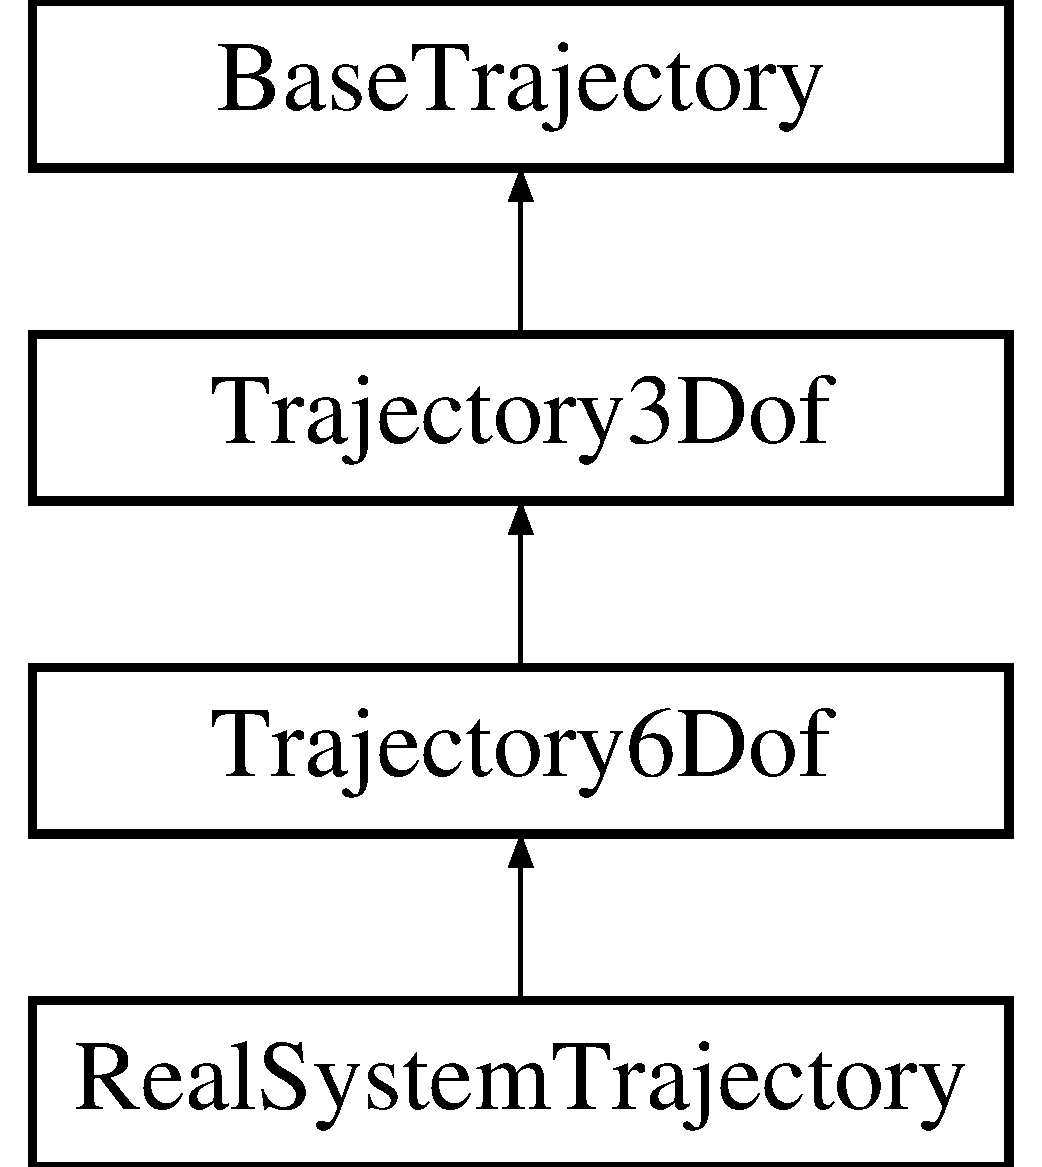
\includegraphics[height=4.000000cm]{class_base_trajectory}
\end{center}
\end{figure}
\subsection*{Public Member Functions}
\begin{DoxyCompactItemize}
\item 
\hyperlink{class_base_trajectory_adeb5dac46dd0e10c53c121abb3cddae2}{Base\+Trajectory} ()
\begin{DoxyCompactList}\small\item\em constructor \end{DoxyCompactList}\item 
\hyperlink{class_base_trajectory_a69beb2e4fc2431d2f150751390bfcfbc}{$\sim$\+Base\+Trajectory} ()
\begin{DoxyCompactList}\small\item\em destructor \end{DoxyCompactList}\item 
virtual void \hyperlink{class_base_trajectory_a4fb09cefd92da44f4e754c8c48f964b5}{init\+Trajectory} (\hyperlink{group___tools_ga3f1431cb9f76da10f59246d1d743dc2c}{Float64} \&Flight\+Time, Aerodynamic\+Struct \&Aero\+Data, Airframe\+Struct \&Airframe\+Data, Thrust\+Struct \&Thrust\+Data, Aircraft\+Struct \&Aircraft\+Data, Guidance\+Struct \&Guidance\+Data, Navigation\+Struct \&Nav\+Data, Actuator\+Struct \&Actuator\+Data, I\+M\+U\+Struct \&I\+M\+U\+Data)
\begin{DoxyCompactList}\small\item\em initalize trajectory \end{DoxyCompactList}\item 
virtual void \hyperlink{class_base_trajectory_a37f0fa46532c754413ee67a846a10624}{update\+Trajectory} (\hyperlink{group___tools_ga3f1431cb9f76da10f59246d1d743dc2c}{Float64} Flight\+Time, Atmosphere\+Struct \&Atmo\+Data, Aerodynamic\+Struct \&Aero\+Data, Airframe\+Struct \&Airframe\+Data, Thrust\+Struct \&Thrust\+Data, Guidance\+Struct \&Guidance\+Data, Navigation\+Struct \&Nav\+Data, Actuator\+Struct \&Actuator\+Data, I\+M\+U\+Struct \&I\+M\+U\+Data)
\begin{DoxyCompactList}\small\item\em calculate trajectory \end{DoxyCompactList}\item 
virtual void \hyperlink{class_base_trajectory_a9e24dc7f487ea46621bd231e9d4d995c}{log\+Traj} ()
\begin{DoxyCompactList}\small\item\em log trajectory data \end{DoxyCompactList}\end{DoxyCompactItemize}


\subsection{Detailed Description}
\begin{DoxyAuthor}{Author}
Jan Olucak 
\end{DoxyAuthor}
\begin{DoxyDate}{Date}
28.\+11.\+2017 
\end{DoxyDate}
\begin{DoxyVersion}{Version}
1.\+0
\end{DoxyVersion}
\hyperlink{class_base_trajectory}{Base\+Trajectory} is the superclass for all trajectory classes. 

Definition at line 14 of file Base\+Trajectory.\+h.



\subsection{Constructor \& Destructor Documentation}
\mbox{\Hypertarget{class_base_trajectory_adeb5dac46dd0e10c53c121abb3cddae2}\label{class_base_trajectory_adeb5dac46dd0e10c53c121abb3cddae2}} 
\index{Base\+Trajectory@{Base\+Trajectory}!Base\+Trajectory@{Base\+Trajectory}}
\index{Base\+Trajectory@{Base\+Trajectory}!Base\+Trajectory@{Base\+Trajectory}}
\subsubsection{\texorpdfstring{Base\+Trajectory()}{BaseTrajectory()}}
{\footnotesize\ttfamily Base\+Trajectory\+::\+Base\+Trajectory (\begin{DoxyParamCaption}{ }\end{DoxyParamCaption})}



constructor 



Definition at line 3 of file Base\+Trajectory.\+cpp.

\mbox{\Hypertarget{class_base_trajectory_a69beb2e4fc2431d2f150751390bfcfbc}\label{class_base_trajectory_a69beb2e4fc2431d2f150751390bfcfbc}} 
\index{Base\+Trajectory@{Base\+Trajectory}!````~Base\+Trajectory@{$\sim$\+Base\+Trajectory}}
\index{````~Base\+Trajectory@{$\sim$\+Base\+Trajectory}!Base\+Trajectory@{Base\+Trajectory}}
\subsubsection{\texorpdfstring{$\sim$\+Base\+Trajectory()}{~BaseTrajectory()}}
{\footnotesize\ttfamily Base\+Trajectory\+::$\sim$\+Base\+Trajectory (\begin{DoxyParamCaption}{ }\end{DoxyParamCaption})}



destructor 



Definition at line 7 of file Base\+Trajectory.\+cpp.



\subsection{Member Function Documentation}
\mbox{\Hypertarget{class_base_trajectory_a4fb09cefd92da44f4e754c8c48f964b5}\label{class_base_trajectory_a4fb09cefd92da44f4e754c8c48f964b5}} 
\index{Base\+Trajectory@{Base\+Trajectory}!init\+Trajectory@{init\+Trajectory}}
\index{init\+Trajectory@{init\+Trajectory}!Base\+Trajectory@{Base\+Trajectory}}
\subsubsection{\texorpdfstring{init\+Trajectory()}{initTrajectory()}}
{\footnotesize\ttfamily void Base\+Trajectory\+::init\+Trajectory (\begin{DoxyParamCaption}\item[{\hyperlink{group___tools_ga3f1431cb9f76da10f59246d1d743dc2c}{Float64} \&}]{Flight\+Time,  }\item[{Aerodynamic\+Struct \&}]{Aero\+Data,  }\item[{Airframe\+Struct \&}]{Airframe\+Data,  }\item[{Thrust\+Struct \&}]{Thrust\+Data,  }\item[{Aircraft\+Struct \&}]{Aircraft\+Data,  }\item[{Guidance\+Struct \&}]{Guidance\+Data,  }\item[{Navigation\+Struct \&}]{Nav\+Data,  }\item[{Actuator\+Struct \&}]{Actuator\+Data,  }\item[{I\+M\+U\+Struct \&}]{I\+M\+U\+Data }\end{DoxyParamCaption})\hspace{0.3cm}{\ttfamily [virtual]}}



initalize trajectory 


\begin{DoxyParams}{Parameters}
{\em Flight\+Time} & flight time \\
\hline
{\em Aero\+Data} & aerodynamic data \\
\hline
{\em Airframe\+Data} & flight states \\
\hline
{\em Thrust\+Data} & thrust forces and moments \\
\hline
{\em Aircraft\+Data} & geometric data of aircraft \\
\hline
{\em Guidance\+Data} & control variables \\
\hline
{\em Nav\+Data} & aircraft position, velocity \\
\hline
{\em Actuator\+Data} & real actuator angles \\
\hline
{\em I\+M\+U\+Data} & measured acceleration \\
\hline
\end{DoxyParams}


Reimplemented in \hyperlink{class_real_system_trajectory_a41ae049eeff69ea6b9daef8027a142a3}{Real\+System\+Trajectory}, \hyperlink{class_trajectory6_dof_a4e81b667130462a85ce047d4942b794c}{Trajectory6\+Dof}, and \hyperlink{class_trajectory3_dof_ab132d729efaded8c7942d462d69cba62}{Trajectory3\+Dof}.



Definition at line 11 of file Base\+Trajectory.\+cpp.



Referenced by Trajectory\+::init\+Trajectory().

\mbox{\Hypertarget{class_base_trajectory_a9e24dc7f487ea46621bd231e9d4d995c}\label{class_base_trajectory_a9e24dc7f487ea46621bd231e9d4d995c}} 
\index{Base\+Trajectory@{Base\+Trajectory}!log\+Traj@{log\+Traj}}
\index{log\+Traj@{log\+Traj}!Base\+Trajectory@{Base\+Trajectory}}
\subsubsection{\texorpdfstring{log\+Traj()}{logTraj()}}
{\footnotesize\ttfamily void Base\+Trajectory\+::log\+Traj (\begin{DoxyParamCaption}{ }\end{DoxyParamCaption})\hspace{0.3cm}{\ttfamily [virtual]}}



log trajectory data 



Definition at line 37 of file Base\+Trajectory.\+cpp.



Referenced by Trajectory\+::log\+Traj().

\mbox{\Hypertarget{class_base_trajectory_a37f0fa46532c754413ee67a846a10624}\label{class_base_trajectory_a37f0fa46532c754413ee67a846a10624}} 
\index{Base\+Trajectory@{Base\+Trajectory}!update\+Trajectory@{update\+Trajectory}}
\index{update\+Trajectory@{update\+Trajectory}!Base\+Trajectory@{Base\+Trajectory}}
\subsubsection{\texorpdfstring{update\+Trajectory()}{updateTrajectory()}}
{\footnotesize\ttfamily void Base\+Trajectory\+::update\+Trajectory (\begin{DoxyParamCaption}\item[{\hyperlink{group___tools_ga3f1431cb9f76da10f59246d1d743dc2c}{Float64}}]{Flight\+Time,  }\item[{Atmosphere\+Struct \&}]{Atmo\+Data,  }\item[{Aerodynamic\+Struct \&}]{Aero\+Data,  }\item[{Airframe\+Struct \&}]{Airframe\+Data,  }\item[{Thrust\+Struct \&}]{Thrust\+Data,  }\item[{Guidance\+Struct \&}]{Guidance\+Data,  }\item[{Navigation\+Struct \&}]{Nav\+Data,  }\item[{Actuator\+Struct \&}]{Actuator\+Data,  }\item[{I\+M\+U\+Struct \&}]{I\+M\+U\+Data }\end{DoxyParamCaption})\hspace{0.3cm}{\ttfamily [virtual]}}



calculate trajectory 


\begin{DoxyParams}{Parameters}
{\em Flight\+Time} & flight time \\
\hline
{\em Atmo\+Data} & current atmospheric data \\
\hline
{\em Aero\+Data} & aerodynamic data \\
\hline
{\em Airframe\+Data} & flight states \\
\hline
{\em Thrust\+Data} & thrust forces and moments \\
\hline
{\em Guidance\+Data} & control variables \\
\hline
{\em Nav\+Data} & aircraft position, velocity \\
\hline
{\em Actuator\+Data} & real actuator angles \\
\hline
{\em I\+M\+U\+Data} & measured acceleration \\
\hline
\end{DoxyParams}


Reimplemented in \hyperlink{class_trajectory6_dof_aafe86c414f4717075a3e0f40c0543fa1}{Trajectory6\+Dof}, \hyperlink{class_real_system_trajectory_a16cace4a95283499ffe59dccabff4c68}{Real\+System\+Trajectory}, and \hyperlink{class_trajectory3_dof_a286d578ad75beaf1018350167557a457}{Trajectory3\+Dof}.



Definition at line 24 of file Base\+Trajectory.\+cpp.



Referenced by Trajectory\+::update\+Trajectory().



The documentation for this class was generated from the following files\+:\begin{DoxyCompactItemize}
\item 
C\+:/\+Users/janol/\+Desktop/\+Simulation\+\_\+\+Stand230618/\+Trajectory/\hyperlink{_base_trajectory_8h}{Base\+Trajectory.\+h}\item 
C\+:/\+Users/janol/\+Desktop/\+Simulation\+\_\+\+Stand230618/\+Trajectory/\hyperlink{_base_trajectory_8cpp}{Base\+Trajectory.\+cpp}\end{DoxyCompactItemize}

\hypertarget{class_data_logger}{}\section{Data\+Logger Class Reference}
\label{class_data_logger}\index{Data\+Logger@{Data\+Logger}}
\subsection*{Public Member Functions}
\begin{DoxyCompactItemize}
\item 
\mbox{\Hypertarget{class_data_logger_aa95dc52c00e81fcb074ef4224d305238}\label{class_data_logger_aa95dc52c00e81fcb074ef4224d305238}} 
{\bfseries Data\+Logger} (std\+::string a\+Path, int a\+Width, std\+::string a\+Delimiter)
\item 
\mbox{\Hypertarget{class_data_logger_a31d8ed8cfdda531f19236e214d5d931f}\label{class_data_logger_a31d8ed8cfdda531f19236e214d5d931f}} 
void {\bfseries add} (std\+::string a\+Header, double \&a\+Var)
\item 
\mbox{\Hypertarget{class_data_logger_a9af9879fe968dee468b3e479cadf073a}\label{class_data_logger_a9af9879fe968dee468b3e479cadf073a}} 
void {\bfseries add} (std\+::string a\+Header, int \&a\+Var)
\item 
\mbox{\Hypertarget{class_data_logger_aa1bd66fc07169787398f386d9276708b}\label{class_data_logger_aa1bd66fc07169787398f386d9276708b}} 
void {\bfseries print} ()
\item 
\mbox{\Hypertarget{class_data_logger_ad7247b2350411b48f323de6c91e8479c}\label{class_data_logger_ad7247b2350411b48f323de6c91e8479c}} 
void {\bfseries print\+Header} ()
\end{DoxyCompactItemize}


\subsection{Detailed Description}


Definition at line \hyperlink{_data_logger_8h_source_l00009}{9} of file \hyperlink{_data_logger_8h_source}{Data\+Logger.\+h}.



The documentation for this class was generated from the following files\+:\begin{DoxyCompactItemize}
\item 
Data\+Logger.\+h\item 
Data\+Logger.\+cpp\end{DoxyCompactItemize}

\hypertarget{class_d_a_t_c_o_m_aerodymamic}{}\section{D\+A\+T\+C\+O\+M\+Aerodymamic Class Reference}
\label{class_d_a_t_c_o_m_aerodymamic}\index{D\+A\+T\+C\+O\+M\+Aerodymamic@{D\+A\+T\+C\+O\+M\+Aerodymamic}}


{\ttfamily \#include $<$D\+A\+T\+C\+O\+M\+Aerodynamic.\+h$>$}

Inheritance diagram for D\+A\+T\+C\+O\+M\+Aerodymamic\+:\begin{figure}[H]
\begin{center}
\leavevmode
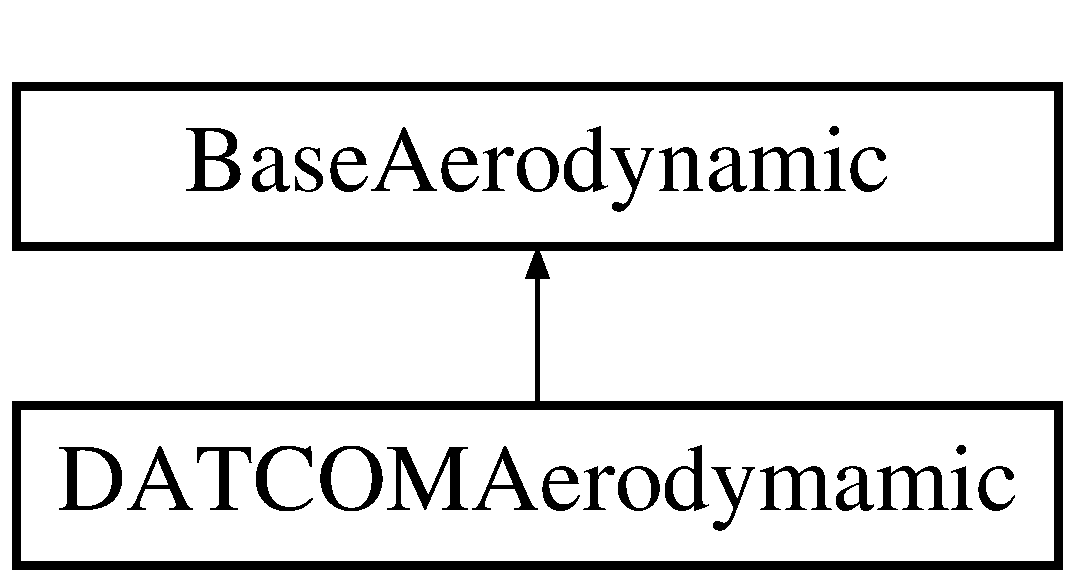
\includegraphics[height=2.000000cm]{class_d_a_t_c_o_m_aerodymamic}
\end{center}
\end{figure}
\subsection*{Public Member Functions}
\begin{DoxyCompactItemize}
\item 
\hyperlink{class_d_a_t_c_o_m_aerodymamic_a03d01a72cf389483e03e2bf6cce33299}{D\+A\+T\+C\+O\+M\+Aerodymamic} ()
\begin{DoxyCompactList}\small\item\em constructor \end{DoxyCompactList}\item 
\hyperlink{class_d_a_t_c_o_m_aerodymamic_a3619e38867cad4b0c8b06a939281a74e}{$\sim$\+D\+A\+T\+C\+O\+M\+Aerodymamic} ()
\begin{DoxyCompactList}\small\item\em destructor \end{DoxyCompactList}\item 
void \hyperlink{class_d_a_t_c_o_m_aerodymamic_aa4909fb5e6db41f2309b7d8a8658a219}{init\+Aerodynamic} (\hyperlink{group___tools_ga3f1431cb9f76da10f59246d1d743dc2c}{Float64} \&Flight\+Time, Aerodynamic\+Struct \&Aero\+Data, Aircraft\+Struct \&Aircraft\+Data)
\begin{DoxyCompactList}\small\item\em read in tables of derivatives \end{DoxyCompactList}\item 
void \hyperlink{class_d_a_t_c_o_m_aerodymamic_a501386a4e5d176d3fb8bddae1d0c8d0f}{update\+Aerodynamic} (\hyperlink{group___tools_ga3f1431cb9f76da10f59246d1d743dc2c}{Float64} Flight\+Time, Atmosphere\+Struct \&Atmo\+Data, Aerodynamic\+Struct \&Aero\+Data, Airframe\+Struct \&Airframe\+Data, Thrust\+Struct \&Thrust\+Data, Actuator\+Struct \&Actuator\+Data, I\+M\+U\+Struct \&I\+M\+U\+Data, Navigation\+Struct \&Nav\+Data)
\begin{DoxyCompactList}\small\item\em current flight state is used to interpolated derivatives and a linear aerodynamic model calculates forces and moments \end{DoxyCompactList}\item 
virtual void \hyperlink{class_d_a_t_c_o_m_aerodymamic_a5bf2796685504755b9d23cb8cfd90752}{init\+Log\+Aero\+Data} (\hyperlink{group___tools_ga3f1431cb9f76da10f59246d1d743dc2c}{Float64} \&Flight\+Time, Aerodynamic\+Struct \&Aero\+Data)
\begin{DoxyCompactList}\small\item\em definition of data which is logged to an outputfile \end{DoxyCompactList}\item 
void \hyperlink{class_d_a_t_c_o_m_aerodymamic_a84ab90acbbec700e0b06272bf95cf932}{Log\+Aero\+Data} ()
\begin{DoxyCompactList}\small\item\em logging of aerodynamic data \end{DoxyCompactList}\end{DoxyCompactItemize}


\subsection{Detailed Description}
\begin{DoxyAuthor}{Author}
Jan Olucak 
\end{DoxyAuthor}
\begin{DoxyDate}{Date}
25.\+11.\+2017 
\end{DoxyDate}
\begin{DoxyVersion}{Version}
1.\+0
\end{DoxyVersion}
D\+A\+T\+C\+OM aerodynamic class is a child class from \hyperlink{class_base_aerodynamic}{Base\+Aerodynamic}. This class calculates aerodynamic forces and moments with tables from D\+A\+T\+C\+OM. Tables of derivative are read in from specific file. 

Definition at line 25 of file D\+A\+T\+C\+O\+M\+Aerodynamic.\+h.



\subsection{Constructor \& Destructor Documentation}
\mbox{\Hypertarget{class_d_a_t_c_o_m_aerodymamic_a03d01a72cf389483e03e2bf6cce33299}\label{class_d_a_t_c_o_m_aerodymamic_a03d01a72cf389483e03e2bf6cce33299}} 
\index{D\+A\+T\+C\+O\+M\+Aerodymamic@{D\+A\+T\+C\+O\+M\+Aerodymamic}!D\+A\+T\+C\+O\+M\+Aerodymamic@{D\+A\+T\+C\+O\+M\+Aerodymamic}}
\index{D\+A\+T\+C\+O\+M\+Aerodymamic@{D\+A\+T\+C\+O\+M\+Aerodymamic}!D\+A\+T\+C\+O\+M\+Aerodymamic@{D\+A\+T\+C\+O\+M\+Aerodymamic}}
\subsubsection{\texorpdfstring{D\+A\+T\+C\+O\+M\+Aerodymamic()}{DATCOMAerodymamic()}}
{\footnotesize\ttfamily D\+A\+T\+C\+O\+M\+Aerodymamic\+::\+D\+A\+T\+C\+O\+M\+Aerodymamic (\begin{DoxyParamCaption}{ }\end{DoxyParamCaption})}



constructor 



Definition at line 3 of file D\+A\+T\+C\+O\+M\+Aerodynamic.\+cpp.

\mbox{\Hypertarget{class_d_a_t_c_o_m_aerodymamic_a3619e38867cad4b0c8b06a939281a74e}\label{class_d_a_t_c_o_m_aerodymamic_a3619e38867cad4b0c8b06a939281a74e}} 
\index{D\+A\+T\+C\+O\+M\+Aerodymamic@{D\+A\+T\+C\+O\+M\+Aerodymamic}!````~D\+A\+T\+C\+O\+M\+Aerodymamic@{$\sim$\+D\+A\+T\+C\+O\+M\+Aerodymamic}}
\index{````~D\+A\+T\+C\+O\+M\+Aerodymamic@{$\sim$\+D\+A\+T\+C\+O\+M\+Aerodymamic}!D\+A\+T\+C\+O\+M\+Aerodymamic@{D\+A\+T\+C\+O\+M\+Aerodymamic}}
\subsubsection{\texorpdfstring{$\sim$\+D\+A\+T\+C\+O\+M\+Aerodymamic()}{~DATCOMAerodymamic()}}
{\footnotesize\ttfamily D\+A\+T\+C\+O\+M\+Aerodymamic\+::$\sim$\+D\+A\+T\+C\+O\+M\+Aerodymamic (\begin{DoxyParamCaption}{ }\end{DoxyParamCaption})}



destructor 



Definition at line 10 of file D\+A\+T\+C\+O\+M\+Aerodynamic.\+cpp.



\subsection{Member Function Documentation}
\mbox{\Hypertarget{class_d_a_t_c_o_m_aerodymamic_aa4909fb5e6db41f2309b7d8a8658a219}\label{class_d_a_t_c_o_m_aerodymamic_aa4909fb5e6db41f2309b7d8a8658a219}} 
\index{D\+A\+T\+C\+O\+M\+Aerodymamic@{D\+A\+T\+C\+O\+M\+Aerodymamic}!init\+Aerodynamic@{init\+Aerodynamic}}
\index{init\+Aerodynamic@{init\+Aerodynamic}!D\+A\+T\+C\+O\+M\+Aerodymamic@{D\+A\+T\+C\+O\+M\+Aerodymamic}}
\subsubsection{\texorpdfstring{init\+Aerodynamic()}{initAerodynamic()}}
{\footnotesize\ttfamily void D\+A\+T\+C\+O\+M\+Aerodymamic\+::init\+Aerodynamic (\begin{DoxyParamCaption}\item[{\hyperlink{group___tools_ga3f1431cb9f76da10f59246d1d743dc2c}{Float64} \&}]{Flight\+Time,  }\item[{Aerodynamic\+Struct \&}]{Aero\+Data,  }\item[{Aircraft\+Struct \&}]{Aircraft\+Data }\end{DoxyParamCaption})\hspace{0.3cm}{\ttfamily [virtual]}}



read in tables of derivatives 


\begin{DoxyParams}{Parameters}
{\em Flight\+Time} & flighttime \\
\hline
{\em Aero\+Data} & structure of aero data \\
\hline
{\em Aircraft\+Data} & structure of aircraft data \\
\hline
\end{DoxyParams}
1) read in tables of aerdynamic derivatives 

Reimplemented from \hyperlink{class_base_aerodynamic_a6493b7d9c4cbadcbf3a8e5a6c973e1f3}{Base\+Aerodynamic}.



Definition at line 14 of file D\+A\+T\+C\+O\+M\+Aerodynamic.\+cpp.

\mbox{\Hypertarget{class_d_a_t_c_o_m_aerodymamic_a5bf2796685504755b9d23cb8cfd90752}\label{class_d_a_t_c_o_m_aerodymamic_a5bf2796685504755b9d23cb8cfd90752}} 
\index{D\+A\+T\+C\+O\+M\+Aerodymamic@{D\+A\+T\+C\+O\+M\+Aerodymamic}!init\+Log\+Aero\+Data@{init\+Log\+Aero\+Data}}
\index{init\+Log\+Aero\+Data@{init\+Log\+Aero\+Data}!D\+A\+T\+C\+O\+M\+Aerodymamic@{D\+A\+T\+C\+O\+M\+Aerodymamic}}
\subsubsection{\texorpdfstring{init\+Log\+Aero\+Data()}{initLogAeroData()}}
{\footnotesize\ttfamily void D\+A\+T\+C\+O\+M\+Aerodymamic\+::init\+Log\+Aero\+Data (\begin{DoxyParamCaption}\item[{\hyperlink{group___tools_ga3f1431cb9f76da10f59246d1d743dc2c}{Float64} \&}]{Flight\+Time,  }\item[{Aerodynamic\+Struct \&}]{Aero\+Data }\end{DoxyParamCaption})\hspace{0.3cm}{\ttfamily [virtual]}}



definition of data which is logged to an outputfile 


\begin{DoxyParams}{Parameters}
{\em Flight\+Time} & time of flight \\
\hline
{\em Aero\+Data} & structure of aerodynamic data \\
\hline
\end{DoxyParams}


Definition at line 192 of file D\+A\+T\+C\+O\+M\+Aerodynamic.\+cpp.



Referenced by init\+Aerodynamic().

\mbox{\Hypertarget{class_d_a_t_c_o_m_aerodymamic_a84ab90acbbec700e0b06272bf95cf932}\label{class_d_a_t_c_o_m_aerodymamic_a84ab90acbbec700e0b06272bf95cf932}} 
\index{D\+A\+T\+C\+O\+M\+Aerodymamic@{D\+A\+T\+C\+O\+M\+Aerodymamic}!Log\+Aero\+Data@{Log\+Aero\+Data}}
\index{Log\+Aero\+Data@{Log\+Aero\+Data}!D\+A\+T\+C\+O\+M\+Aerodymamic@{D\+A\+T\+C\+O\+M\+Aerodymamic}}
\subsubsection{\texorpdfstring{Log\+Aero\+Data()}{LogAeroData()}}
{\footnotesize\ttfamily void D\+A\+T\+C\+O\+M\+Aerodymamic\+::\+Log\+Aero\+Data (\begin{DoxyParamCaption}{ }\end{DoxyParamCaption})\hspace{0.3cm}{\ttfamily [virtual]}}



logging of aerodynamic data 



Reimplemented from \hyperlink{class_base_aerodynamic_abaea76739e197627a6d09cff5b68af83}{Base\+Aerodynamic}.



Definition at line 208 of file D\+A\+T\+C\+O\+M\+Aerodynamic.\+cpp.

\mbox{\Hypertarget{class_d_a_t_c_o_m_aerodymamic_a501386a4e5d176d3fb8bddae1d0c8d0f}\label{class_d_a_t_c_o_m_aerodymamic_a501386a4e5d176d3fb8bddae1d0c8d0f}} 
\index{D\+A\+T\+C\+O\+M\+Aerodymamic@{D\+A\+T\+C\+O\+M\+Aerodymamic}!update\+Aerodynamic@{update\+Aerodynamic}}
\index{update\+Aerodynamic@{update\+Aerodynamic}!D\+A\+T\+C\+O\+M\+Aerodymamic@{D\+A\+T\+C\+O\+M\+Aerodymamic}}
\subsubsection{\texorpdfstring{update\+Aerodynamic()}{updateAerodynamic()}}
{\footnotesize\ttfamily void D\+A\+T\+C\+O\+M\+Aerodymamic\+::update\+Aerodynamic (\begin{DoxyParamCaption}\item[{\hyperlink{group___tools_ga3f1431cb9f76da10f59246d1d743dc2c}{Float64}}]{Flight\+Time,  }\item[{Atmosphere\+Struct \&}]{Atmo\+Data,  }\item[{Aerodynamic\+Struct \&}]{Aero\+Data,  }\item[{Airframe\+Struct \&}]{Airframe\+Data,  }\item[{Thrust\+Struct \&}]{Thrust\+Data,  }\item[{Actuator\+Struct \&}]{Actuator\+Data,  }\item[{I\+M\+U\+Struct \&}]{I\+M\+U\+Data,  }\item[{Navigation\+Struct \&}]{Nav\+Data }\end{DoxyParamCaption})\hspace{0.3cm}{\ttfamily [virtual]}}



current flight state is used to interpolated derivatives and a linear aerodynamic model calculates forces and moments 


\begin{DoxyParams}{Parameters}
{\em Flight\+Time} & Flight Time \\
\hline
{\em Atmo\+Data} & air density, speed of sound \\
\hline
{\em Aero\+Data} & structure of aero data \\
\hline
{\em Airframe\+Data} & structure of airframe data \\
\hline
{\em Thrust\+Data} & structure of thrust data \\
\hline
{\em Actuator\+Data} & actuator angles \\
\hline
{\em I\+M\+U\+Data} & rotational rates \\
\hline
{\em Nav\+Data} & \hyperlink{class_navigation}{Navigation} data like velocity in N\+ED system \\
\hline
\end{DoxyParams}
1) get data from structures

2) depending on flight states interpolate derivatives

3) calculate aerodynamic coefficients

4) calculate derivatives for acceleration table guidance

5) store data to aerodynamic struct 

Reimplemented from \hyperlink{class_base_aerodynamic_a8a417495c896359b2ee74f5c1c8c08f7}{Base\+Aerodynamic}.



Definition at line 68 of file D\+A\+T\+C\+O\+M\+Aerodynamic.\+cpp.



The documentation for this class was generated from the following files\+:\begin{DoxyCompactItemize}
\item 
C\+:/\+Users/janol/\+Desktop/\+Simulation\+\_\+\+Stand230618/\+Aerodynamic/\hyperlink{_d_a_t_c_o_m_aerodynamic_8h}{D\+A\+T\+C\+O\+M\+Aerodynamic.\+h}\item 
C\+:/\+Users/janol/\+Desktop/\+Simulation\+\_\+\+Stand230618/\+Aerodynamic/\hyperlink{_d_a_t_c_o_m_aerodynamic_8cpp}{D\+A\+T\+C\+O\+M\+Aerodynamic.\+cpp}\end{DoxyCompactItemize}

\hypertarget{class_engine}{}\section{Engine Class Reference}
\label{class_engine}\index{Engine@{Engine}}
\subsection*{Public Member Functions}
\begin{DoxyCompactItemize}
\item 
\mbox{\Hypertarget{class_engine_ac33371d6fff86c0c8e14495f10046d9a}\label{class_engine_ac33371d6fff86c0c8e14495f10046d9a}} 
void {\bfseries select\+Engine\+Type} (int type)
\item 
\mbox{\Hypertarget{class_engine_aca6cc0dc7d537295123630a219142337}\label{class_engine_aca6cc0dc7d537295123630a219142337}} 
void {\bfseries init\+Engine} ()
\item 
\mbox{\Hypertarget{class_engine_a9e16100ffd33cf8ec632257795c03865}\label{class_engine_a9e16100ffd33cf8ec632257795c03865}} 
void {\bfseries update\+Engine} (Float64 Flight\+Time, \hyperlink{group___data_cloud_struct_atmosphere_struct}{Atmosphere\+Struct} \&Atmo\+Data, \hyperlink{group___data_cloud_struct_aerodynamic_struct}{Aerodynamic\+Struct} \&Aero\+Data, \hyperlink{group___data_cloud_struct_airframe_struct}{Airframe\+Struct} \&Airframe\+Data, \hyperlink{group___data_cloud_struct_thrust_struct}{Thrust\+Struct} \&Thrust\+Data)
\end{DoxyCompactItemize}


The documentation for this class was generated from the following files\+:\begin{DoxyCompactItemize}
\item 
Engine.\+h\item 
Engine.\+cpp\end{DoxyCompactItemize}

\hypertarget{class_find_neighbor}{}\section{Find\+Neighbor Class Reference}
\label{class_find_neighbor}\index{Find\+Neighbor@{Find\+Neighbor}}
\subsection*{Public Member Functions}
\begin{DoxyCompactItemize}
\item 
\mbox{\Hypertarget{class_find_neighbor_a749dad6095d8e0e62dd5ba11abdd7500}\label{class_find_neighbor_a749dad6095d8e0e62dd5ba11abdd7500}} 
void {\bfseries init\+Find\+Neighbor} ()
\item 
\mbox{\Hypertarget{class_find_neighbor_a661260e53f2343fb679f3eefc8f5f02e}\label{class_find_neighbor_a661260e53f2343fb679f3eefc8f5f02e}} 
Eigen\+::\+Vector4d {\bfseries Blending\+Parameters} (Airframe\+Struct \&Airframe\+Data)
\item 
\mbox{\Hypertarget{class_find_neighbor_ac0133668987495831b577fefb8bdca50}\label{class_find_neighbor_ac0133668987495831b577fefb8bdca50}} 
Eigen\+::\+Matrix\+Xd {\bfseries combine\+Vec} (Eigen\+::\+Vector2d \&Alt, Eigen\+::\+Vector2d \&Vel)
\end{DoxyCompactItemize}


\subsection{Detailed Description}


Definition at line \hyperlink{_find_neighbor_8h_source_l00010}{10} of file \hyperlink{_find_neighbor_8h_source}{Find\+Neighbor.\+h}.



The documentation for this class was generated from the following files\+:\begin{DoxyCompactItemize}
\item 
Find\+Neighbor.\+h\item 
Find\+Neighbor.\+cpp\end{DoxyCompactItemize}

\hypertarget{classflawless_actuator}{}\section{flawless\+Actuator Class Reference}
\label{classflawless_actuator}\index{flawless\+Actuator@{flawless\+Actuator}}


{\ttfamily \#include $<$flawless\+Actuator.\+h$>$}

Inheritance diagram for flawless\+Actuator\+:\begin{figure}[H]
\begin{center}
\leavevmode
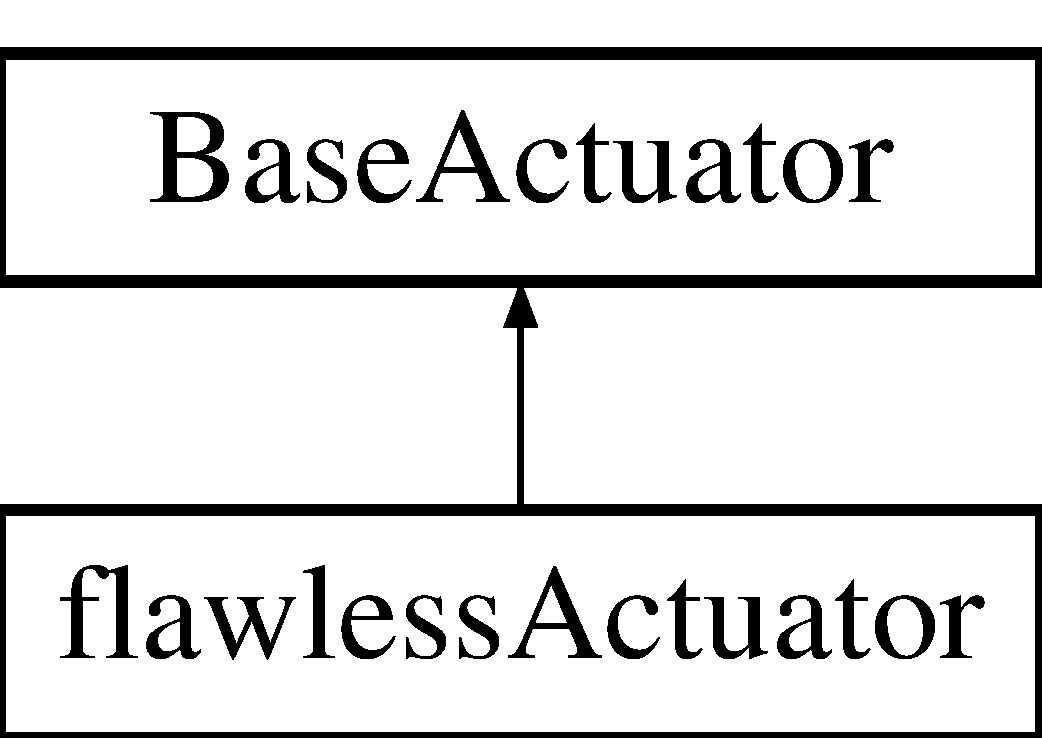
\includegraphics[height=2.000000cm]{classflawless_actuator}
\end{center}
\end{figure}
\subsection*{Public Member Functions}
\begin{DoxyCompactItemize}
\item 
\hyperlink{classflawless_actuator_a73fc69c36971b5ffc8c9c7d135f1bb30}{flawless\+Actuator} ()
\begin{DoxyCompactList}\small\item\em construtor \end{DoxyCompactList}\item 
\hyperlink{classflawless_actuator_a3a37f5cff70fd61354dc25aa4bfe2466}{$\sim$flawless\+Actuator} ()
\begin{DoxyCompactList}\small\item\em destructor \end{DoxyCompactList}\item 
virtual void \hyperlink{classflawless_actuator_a8676b36d0dfd7c8d7d789bdd6135db8f}{init\+Actuator} (\hyperlink{group___tools_ga3f1431cb9f76da10f59246d1d743dc2c}{Float64} \&Flight\+Time, Airframe\+Struct \&Airframe\+Data, Actuator\+Struct \&Actuator\+Data)
\begin{DoxyCompactList}\small\item\em initialize selected actuator model \end{DoxyCompactList}\item 
virtual void \hyperlink{classflawless_actuator_ad025b033eb040a76cc7d4a7b85ad33da}{update\+Actuator} (\hyperlink{group___tools_ga3f1431cb9f76da10f59246d1d743dc2c}{Float64} Flight\+Time, Airframe\+Struct \&Airframe\+Data, Actuator\+Struct \&Actuator\+Data)
\begin{DoxyCompactList}\small\item\em initialize selected actuator model \end{DoxyCompactList}\item 
void \hyperlink{classflawless_actuator_a10b782f3ece4dff258a4914cdb08d273}{init\+Log\+Actuator\+Data} (\hyperlink{group___tools_ga3f1431cb9f76da10f59246d1d743dc2c}{Float64} \&Flight\+Time, Actuator\+Struct \&Actuator\+Data)
\begin{DoxyCompactList}\small\item\em define parameters for logging \end{DoxyCompactList}\item 
void \hyperlink{classflawless_actuator_a5cd61e149a795ba7db292101d4782bd5}{Log\+Actuator\+Data} ()
\begin{DoxyCompactList}\small\item\em log actuator data \end{DoxyCompactList}\end{DoxyCompactItemize}


\subsection{Detailed Description}
\begin{DoxyAuthor}{Author}
Jan Olucak 
\end{DoxyAuthor}
\begin{DoxyDate}{Date}
25.\+11.\+2017 
\end{DoxyDate}
\begin{DoxyVersion}{Version}
1.\+0
\end{DoxyVersion}
\hyperlink{classflawless_actuator}{flawless\+Actuator} class is inherited from \hyperlink{class_base_actuator}{Base\+Actuator}. It is the simplest model for an actuator 

Definition at line 18 of file flawless\+Actuator.\+h.



\subsection{Constructor \& Destructor Documentation}
\mbox{\Hypertarget{classflawless_actuator_a73fc69c36971b5ffc8c9c7d135f1bb30}\label{classflawless_actuator_a73fc69c36971b5ffc8c9c7d135f1bb30}} 
\index{flawless\+Actuator@{flawless\+Actuator}!flawless\+Actuator@{flawless\+Actuator}}
\index{flawless\+Actuator@{flawless\+Actuator}!flawless\+Actuator@{flawless\+Actuator}}
\subsubsection{\texorpdfstring{flawless\+Actuator()}{flawlessActuator()}}
{\footnotesize\ttfamily flawless\+Actuator\+::flawless\+Actuator (\begin{DoxyParamCaption}{ }\end{DoxyParamCaption})}



construtor 



Definition at line 3 of file flawless\+Actuator.\+cpp.

\mbox{\Hypertarget{classflawless_actuator_a3a37f5cff70fd61354dc25aa4bfe2466}\label{classflawless_actuator_a3a37f5cff70fd61354dc25aa4bfe2466}} 
\index{flawless\+Actuator@{flawless\+Actuator}!````~flawless\+Actuator@{$\sim$flawless\+Actuator}}
\index{````~flawless\+Actuator@{$\sim$flawless\+Actuator}!flawless\+Actuator@{flawless\+Actuator}}
\subsubsection{\texorpdfstring{$\sim$flawless\+Actuator()}{~flawlessActuator()}}
{\footnotesize\ttfamily flawless\+Actuator\+::$\sim$flawless\+Actuator (\begin{DoxyParamCaption}{ }\end{DoxyParamCaption})}



destructor 



Definition at line 8 of file flawless\+Actuator.\+cpp.



\subsection{Member Function Documentation}
\mbox{\Hypertarget{classflawless_actuator_a8676b36d0dfd7c8d7d789bdd6135db8f}\label{classflawless_actuator_a8676b36d0dfd7c8d7d789bdd6135db8f}} 
\index{flawless\+Actuator@{flawless\+Actuator}!init\+Actuator@{init\+Actuator}}
\index{init\+Actuator@{init\+Actuator}!flawless\+Actuator@{flawless\+Actuator}}
\subsubsection{\texorpdfstring{init\+Actuator()}{initActuator()}}
{\footnotesize\ttfamily void flawless\+Actuator\+::init\+Actuator (\begin{DoxyParamCaption}\item[{\hyperlink{group___tools_ga3f1431cb9f76da10f59246d1d743dc2c}{Float64} \&}]{Flight\+Time,  }\item[{Airframe\+Struct \&}]{Airframe\+Data,  }\item[{Actuator\+Struct \&}]{Actuator\+Data }\end{DoxyParamCaption})\hspace{0.3cm}{\ttfamily [virtual]}}



initialize selected actuator model 


\begin{DoxyParams}{Parameters}
{\em Flight\+Time} & Flight time \\
\hline
{\em Airframe\+Data} & coammanded actuator angles from autopilot \\
\hline
{\em Actuator\+Data} & real \hyperlink{class_actuator}{Actuator} angles \\
\hline
\end{DoxyParams}


Reimplemented from \hyperlink{class_base_actuator_aa37ef0301610ceba649c25bdaa71fa87}{Base\+Actuator}.



Definition at line 12 of file flawless\+Actuator.\+cpp.

\mbox{\Hypertarget{classflawless_actuator_a10b782f3ece4dff258a4914cdb08d273}\label{classflawless_actuator_a10b782f3ece4dff258a4914cdb08d273}} 
\index{flawless\+Actuator@{flawless\+Actuator}!init\+Log\+Actuator\+Data@{init\+Log\+Actuator\+Data}}
\index{init\+Log\+Actuator\+Data@{init\+Log\+Actuator\+Data}!flawless\+Actuator@{flawless\+Actuator}}
\subsubsection{\texorpdfstring{init\+Log\+Actuator\+Data()}{initLogActuatorData()}}
{\footnotesize\ttfamily void flawless\+Actuator\+::init\+Log\+Actuator\+Data (\begin{DoxyParamCaption}\item[{\hyperlink{group___tools_ga3f1431cb9f76da10f59246d1d743dc2c}{Float64} \&}]{Flight\+Time,  }\item[{Actuator\+Struct \&}]{Actuator\+Data }\end{DoxyParamCaption})}



define parameters for logging 


\begin{DoxyParams}{Parameters}
{\em Flight\+Time} & Flight time \\
\hline
{\em Actuator\+Data} & real \hyperlink{class_actuator}{Actuator} angles \\
\hline
\end{DoxyParams}


Definition at line 33 of file flawless\+Actuator.\+cpp.



Referenced by init\+Actuator().

\mbox{\Hypertarget{classflawless_actuator_a5cd61e149a795ba7db292101d4782bd5}\label{classflawless_actuator_a5cd61e149a795ba7db292101d4782bd5}} 
\index{flawless\+Actuator@{flawless\+Actuator}!Log\+Actuator\+Data@{Log\+Actuator\+Data}}
\index{Log\+Actuator\+Data@{Log\+Actuator\+Data}!flawless\+Actuator@{flawless\+Actuator}}
\subsubsection{\texorpdfstring{Log\+Actuator\+Data()}{LogActuatorData()}}
{\footnotesize\ttfamily void flawless\+Actuator\+::\+Log\+Actuator\+Data (\begin{DoxyParamCaption}{ }\end{DoxyParamCaption})\hspace{0.3cm}{\ttfamily [virtual]}}



log actuator data 



Reimplemented from \hyperlink{class_base_actuator_a60e40bc448e4bea4e079263dd7d78770}{Base\+Actuator}.



Definition at line 45 of file flawless\+Actuator.\+cpp.

\mbox{\Hypertarget{classflawless_actuator_ad025b033eb040a76cc7d4a7b85ad33da}\label{classflawless_actuator_ad025b033eb040a76cc7d4a7b85ad33da}} 
\index{flawless\+Actuator@{flawless\+Actuator}!update\+Actuator@{update\+Actuator}}
\index{update\+Actuator@{update\+Actuator}!flawless\+Actuator@{flawless\+Actuator}}
\subsubsection{\texorpdfstring{update\+Actuator()}{updateActuator()}}
{\footnotesize\ttfamily void flawless\+Actuator\+::update\+Actuator (\begin{DoxyParamCaption}\item[{\hyperlink{group___tools_ga3f1431cb9f76da10f59246d1d743dc2c}{Float64}}]{Flight\+Time,  }\item[{Airframe\+Struct \&}]{Airframe\+Data,  }\item[{Actuator\+Struct \&}]{Actuator\+Data }\end{DoxyParamCaption})\hspace{0.3cm}{\ttfamily [virtual]}}



initialize selected actuator model 


\begin{DoxyParams}{Parameters}
{\em Flight\+Time} & Flight time \\
\hline
{\em Airframe\+Data} & coammanded actuator angles from autopilot \\
\hline
{\em Actuator\+Data} & real \hyperlink{class_actuator}{Actuator} angles \\
\hline
\end{DoxyParams}


Reimplemented from \hyperlink{class_base_actuator_a8aea3be414ce0dc3afd8e2a54bd523ae}{Base\+Actuator}.



Definition at line 24 of file flawless\+Actuator.\+cpp.



The documentation for this class was generated from the following files\+:\begin{DoxyCompactItemize}
\item 
C\+:/\+Users/janol/\+Desktop/\+Simulation\+\_\+\+Stand230618/\+Actuator/\hyperlink{flawless_actuator_8h}{flawless\+Actuator.\+h}\item 
C\+:/\+Users/janol/\+Desktop/\+Simulation\+\_\+\+Stand230618/\+Actuator/\hyperlink{flawless_actuator_8cpp}{flawless\+Actuator.\+cpp}\end{DoxyCompactItemize}

\hypertarget{classflawless_g_p_s}{}\section{flawless\+G\+PS Class Reference}
\label{classflawless_g_p_s}\index{flawless\+G\+PS@{flawless\+G\+PS}}
Inheritance diagram for flawless\+G\+PS\+:\begin{figure}[H]
\begin{center}
\leavevmode
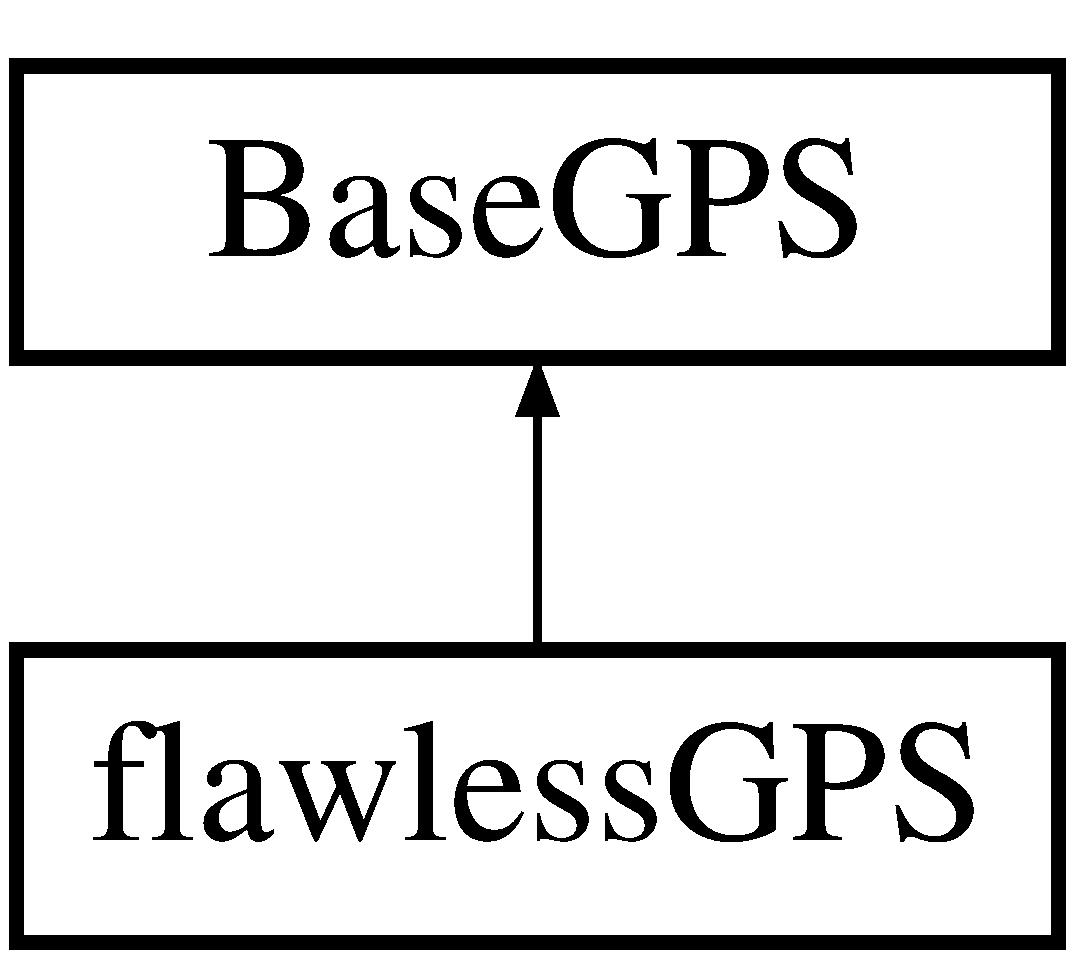
\includegraphics[height=2.000000cm]{classflawless_g_p_s}
\end{center}
\end{figure}
\subsection*{Public Member Functions}
\begin{DoxyCompactItemize}
\item 
\mbox{\Hypertarget{classflawless_g_p_s_a50cdffc0dc65e644f6191bc7c723521b}\label{classflawless_g_p_s_a50cdffc0dc65e644f6191bc7c723521b}} 
void {\bfseries init\+G\+PS} ()
\item 
\mbox{\Hypertarget{classflawless_g_p_s_a09c91bda959ce81236f1f52581ab3bfa}\label{classflawless_g_p_s_a09c91bda959ce81236f1f52581ab3bfa}} 
void {\bfseries update\+G\+PS} (\hyperlink{group___tools_ga3f1431cb9f76da10f59246d1d743dc2c}{Float64} Flight\+Time, Navigation\+Struct \&Nav\+Data)
\end{DoxyCompactItemize}


\subsection{Detailed Description}


Definition at line \hyperlink{flawless_g_p_s_8h_source_l00006}{6} of file \hyperlink{flawless_g_p_s_8h_source}{flawless\+G\+P\+S.\+h}.



The documentation for this class was generated from the following files\+:\begin{DoxyCompactItemize}
\item 
flawless\+G\+P\+S.\+h\item 
flawless\+G\+P\+S.\+cpp\end{DoxyCompactItemize}

\hypertarget{classflawless_i_m_u}{}\section{flawless\+I\+MU Class Reference}
\label{classflawless_i_m_u}\index{flawless\+I\+MU@{flawless\+I\+MU}}
Inheritance diagram for flawless\+I\+MU\+:\begin{figure}[H]
\begin{center}
\leavevmode
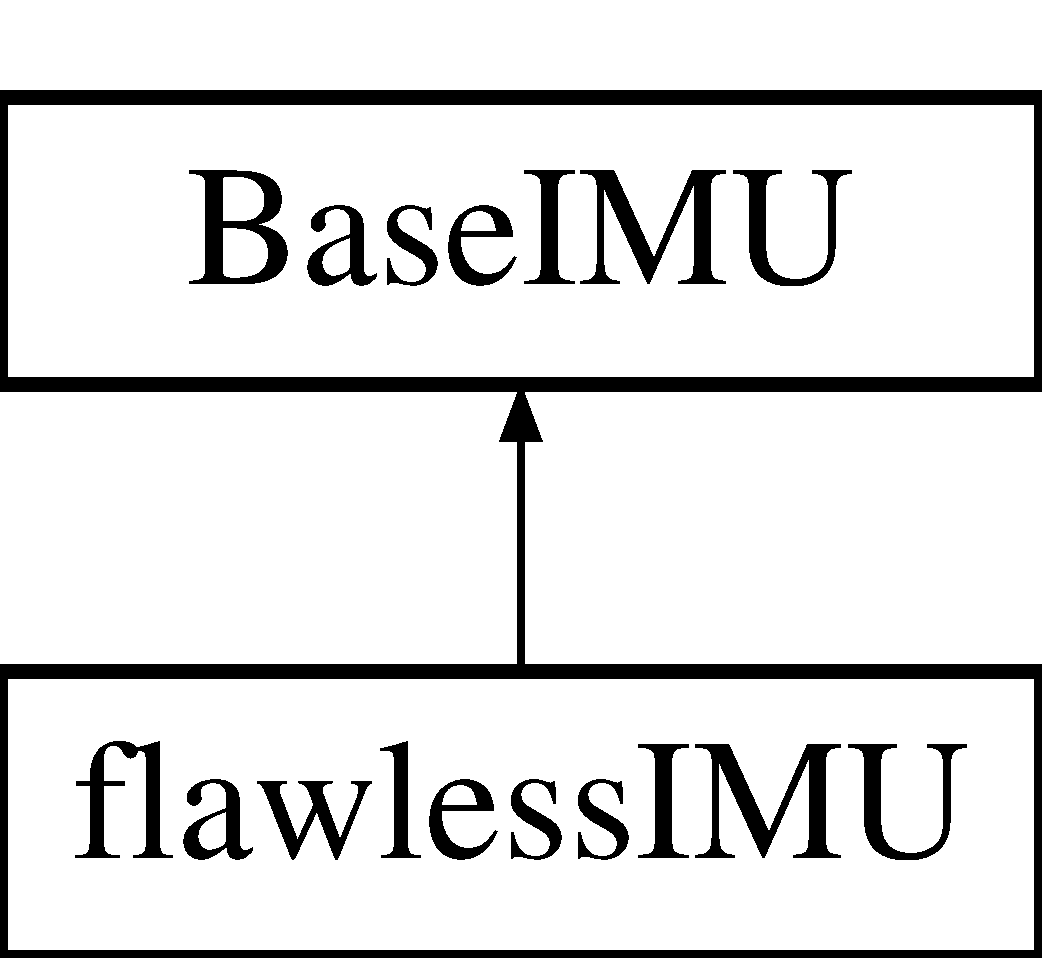
\includegraphics[height=2.000000cm]{classflawless_i_m_u}
\end{center}
\end{figure}
\subsection*{Public Member Functions}
\begin{DoxyCompactItemize}
\item 
\mbox{\Hypertarget{classflawless_i_m_u_a509e17535742d72cf8a4a3ee8b01f5d9}\label{classflawless_i_m_u_a509e17535742d72cf8a4a3ee8b01f5d9}} 
void {\bfseries init\+I\+MU} ()
\item 
\mbox{\Hypertarget{classflawless_i_m_u_a3d3bf018147ba61788fd3e842dded37e}\label{classflawless_i_m_u_a3d3bf018147ba61788fd3e842dded37e}} 
void {\bfseries update\+I\+MU} (\hyperlink{group___tools_ga3f1431cb9f76da10f59246d1d743dc2c}{Float64} Flight\+Time, Airframe\+Struct \&Airframe\+Data, I\+M\+U\+Struct \&I\+M\+U\+Data)
\end{DoxyCompactItemize}


\subsection{Detailed Description}


Definition at line \hyperlink{flawless_i_m_u_8h_source_l00006}{6} of file \hyperlink{flawless_i_m_u_8h_source}{flawless\+I\+M\+U.\+h}.



The documentation for this class was generated from the following files\+:\begin{DoxyCompactItemize}
\item 
flawless\+I\+M\+U.\+h\item 
flawless\+I\+M\+U.\+cpp\end{DoxyCompactItemize}

\hypertarget{classflawless_navigation}{}\section{flawless\+Navigation Class Reference}
\label{classflawless_navigation}\index{flawless\+Navigation@{flawless\+Navigation}}


{\ttfamily \#include $<$flawless\+Navigation.\+h$>$}

Inheritance diagram for flawless\+Navigation\+:\begin{figure}[H]
\begin{center}
\leavevmode
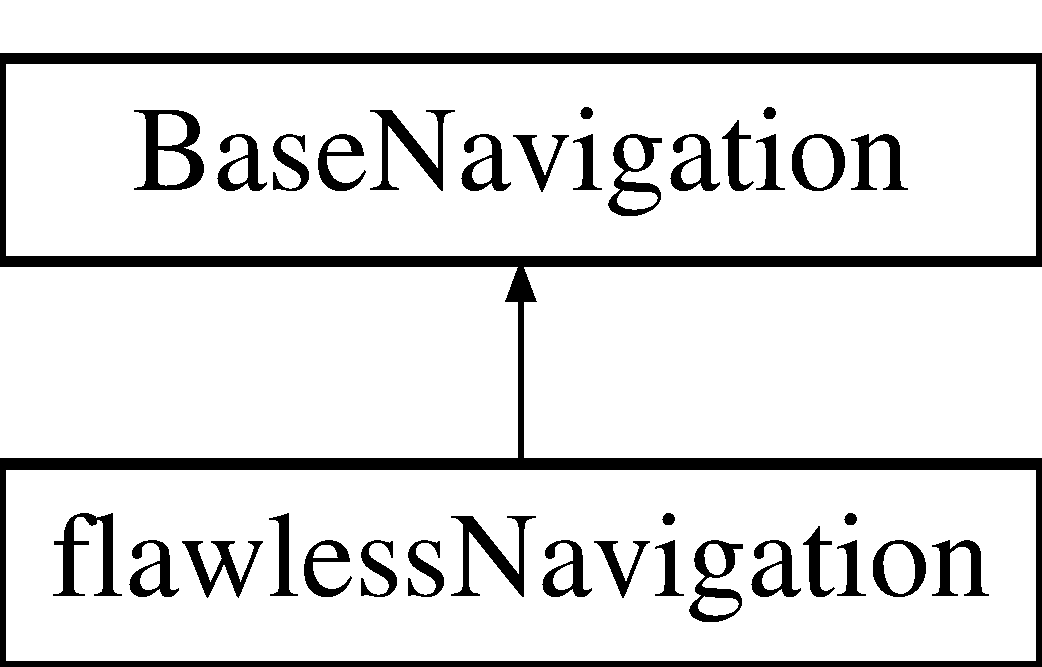
\includegraphics[height=2.000000cm]{classflawless_navigation}
\end{center}
\end{figure}
\subsection*{Public Member Functions}
\begin{DoxyCompactItemize}
\item 
\hyperlink{classflawless_navigation_aaccd796774558ce387216cc539a2eae6}{flawless\+Navigation} ()
\begin{DoxyCompactList}\small\item\em constructor \end{DoxyCompactList}\item 
\hyperlink{classflawless_navigation_af9c6489e6dc05dc5f61646d768de02c0}{$\sim$flawless\+Navigation} ()
\begin{DoxyCompactList}\small\item\em destructor \end{DoxyCompactList}\item 
void \hyperlink{classflawless_navigation_a99e2e982cb7435cbb33533cce1941b39}{init\+Navigation} (\hyperlink{group___tools_ga3f1431cb9f76da10f59246d1d743dc2c}{Float64} \&Flight\+Time, Navigation\+Struct \&Nav\+Data, I\+M\+U\+Struct \&I\+M\+U\+Data)
\begin{DoxyCompactList}\small\item\em initialize flawless navigation \end{DoxyCompactList}\item 
void \hyperlink{classflawless_navigation_ac78ee91130f309c9c5db5bfccd6e8708}{update\+Navigation} (\hyperlink{group___tools_ga3f1431cb9f76da10f59246d1d743dc2c}{Float64} Flight\+Time, Navigation\+Struct \&Nav\+Data, Airframe\+Struct \&Airframe\+Data, I\+M\+U\+Struct \&I\+M\+U\+Data)
\begin{DoxyCompactList}\small\item\em update function of a flawless navigation module \end{DoxyCompactList}\item 
void \hyperlink{classflawless_navigation_a397a8e0d335203cf438a8004370329a5}{initlog\+Navigation\+Data} (\hyperlink{group___tools_ga3f1431cb9f76da10f59246d1d743dc2c}{Float64} \&Flight\+Time, Navigation\+Struct \&Nav\+Data, I\+M\+U\+Struct \&I\+M\+U\+Data)
\begin{DoxyCompactList}\small\item\em data logger for navigation data \end{DoxyCompactList}\item 
void \hyperlink{classflawless_navigation_a0c8ea43db88455be31576a4904f2711e}{log\+Navigation\+Data} ()
\begin{DoxyCompactList}\small\item\em data logger for navigation data \end{DoxyCompactList}\end{DoxyCompactItemize}


\subsection{Detailed Description}
\begin{DoxyAuthor}{Author}
Jan Olucak 
\end{DoxyAuthor}
\begin{DoxyDate}{Date}
02.\+01.\+2018 
\end{DoxyDate}
\begin{DoxyVersion}{Version}
1.\+0
\end{DoxyVersion}
\hyperlink{classflawless_navigation}{flawless\+Navigation} class is a child class of \hyperlink{class_base_navigation}{Base\+Navigation}. A flawless navigation module is simulated. 

Definition at line 16 of file flawless\+Navigation.\+h.



\subsection{Constructor \& Destructor Documentation}
\mbox{\Hypertarget{classflawless_navigation_aaccd796774558ce387216cc539a2eae6}\label{classflawless_navigation_aaccd796774558ce387216cc539a2eae6}} 
\index{flawless\+Navigation@{flawless\+Navigation}!flawless\+Navigation@{flawless\+Navigation}}
\index{flawless\+Navigation@{flawless\+Navigation}!flawless\+Navigation@{flawless\+Navigation}}
\subsubsection{\texorpdfstring{flawless\+Navigation()}{flawlessNavigation()}}
{\footnotesize\ttfamily flawless\+Navigation\+::flawless\+Navigation (\begin{DoxyParamCaption}{ }\end{DoxyParamCaption})}



constructor 



Definition at line 3 of file flawless\+Navigation.\+cpp.

\mbox{\Hypertarget{classflawless_navigation_af9c6489e6dc05dc5f61646d768de02c0}\label{classflawless_navigation_af9c6489e6dc05dc5f61646d768de02c0}} 
\index{flawless\+Navigation@{flawless\+Navigation}!````~flawless\+Navigation@{$\sim$flawless\+Navigation}}
\index{````~flawless\+Navigation@{$\sim$flawless\+Navigation}!flawless\+Navigation@{flawless\+Navigation}}
\subsubsection{\texorpdfstring{$\sim$flawless\+Navigation()}{~flawlessNavigation()}}
{\footnotesize\ttfamily flawless\+Navigation\+::$\sim$flawless\+Navigation (\begin{DoxyParamCaption}{ }\end{DoxyParamCaption})}



destructor 



Definition at line 9 of file flawless\+Navigation.\+cpp.



\subsection{Member Function Documentation}
\mbox{\Hypertarget{classflawless_navigation_a397a8e0d335203cf438a8004370329a5}\label{classflawless_navigation_a397a8e0d335203cf438a8004370329a5}} 
\index{flawless\+Navigation@{flawless\+Navigation}!initlog\+Navigation\+Data@{initlog\+Navigation\+Data}}
\index{initlog\+Navigation\+Data@{initlog\+Navigation\+Data}!flawless\+Navigation@{flawless\+Navigation}}
\subsubsection{\texorpdfstring{initlog\+Navigation\+Data()}{initlogNavigationData()}}
{\footnotesize\ttfamily void flawless\+Navigation\+::initlog\+Navigation\+Data (\begin{DoxyParamCaption}\item[{\hyperlink{group___tools_ga3f1431cb9f76da10f59246d1d743dc2c}{Float64} \&}]{Flight\+Time,  }\item[{Navigation\+Struct \&}]{Nav\+Data,  }\item[{I\+M\+U\+Struct \&}]{I\+M\+U\+Data }\end{DoxyParamCaption})}



data logger for navigation data 


\begin{DoxyParams}{Parameters}
{\em Flight\+Time} & time of flight \\
\hline
{\em Nav\+Data} & solution of navigation estimation \\
\hline
{\em I\+M\+U\+Data} & structure with accelerations and rotatory rates \\
\hline
\end{DoxyParams}


Definition at line 46 of file flawless\+Navigation.\+cpp.



Referenced by init\+Navigation().

\mbox{\Hypertarget{classflawless_navigation_a99e2e982cb7435cbb33533cce1941b39}\label{classflawless_navigation_a99e2e982cb7435cbb33533cce1941b39}} 
\index{flawless\+Navigation@{flawless\+Navigation}!init\+Navigation@{init\+Navigation}}
\index{init\+Navigation@{init\+Navigation}!flawless\+Navigation@{flawless\+Navigation}}
\subsubsection{\texorpdfstring{init\+Navigation()}{initNavigation()}}
{\footnotesize\ttfamily void flawless\+Navigation\+::init\+Navigation (\begin{DoxyParamCaption}\item[{\hyperlink{group___tools_ga3f1431cb9f76da10f59246d1d743dc2c}{Float64} \&}]{Flight\+Time,  }\item[{Navigation\+Struct \&}]{Nav\+Data,  }\item[{I\+M\+U\+Struct \&}]{I\+M\+U\+Data }\end{DoxyParamCaption})\hspace{0.3cm}{\ttfamily [virtual]}}



initialize flawless navigation 


\begin{DoxyParams}{Parameters}
{\em Flight\+Time} & flighttime \\
\hline
{\em Nav\+Data} & structure of position and velocity \\
\hline
{\em I\+M\+U\+Data} & structure with accelerations and rotatory rates \\
\hline
\end{DoxyParams}


Reimplemented from \hyperlink{class_base_navigation_ad447e31e0ee65180872344f2b2a294a8}{Base\+Navigation}.



Definition at line 13 of file flawless\+Navigation.\+cpp.

\mbox{\Hypertarget{classflawless_navigation_a0c8ea43db88455be31576a4904f2711e}\label{classflawless_navigation_a0c8ea43db88455be31576a4904f2711e}} 
\index{flawless\+Navigation@{flawless\+Navigation}!log\+Navigation\+Data@{log\+Navigation\+Data}}
\index{log\+Navigation\+Data@{log\+Navigation\+Data}!flawless\+Navigation@{flawless\+Navigation}}
\subsubsection{\texorpdfstring{log\+Navigation\+Data()}{logNavigationData()}}
{\footnotesize\ttfamily void flawless\+Navigation\+::log\+Navigation\+Data (\begin{DoxyParamCaption}{ }\end{DoxyParamCaption})\hspace{0.3cm}{\ttfamily [virtual]}}



data logger for navigation data 



Reimplemented from \hyperlink{class_base_navigation_ae6974b3c2fb26c03bbf0f2f26b1e9537}{Base\+Navigation}.



Definition at line 66 of file flawless\+Navigation.\+cpp.

\mbox{\Hypertarget{classflawless_navigation_ac78ee91130f309c9c5db5bfccd6e8708}\label{classflawless_navigation_ac78ee91130f309c9c5db5bfccd6e8708}} 
\index{flawless\+Navigation@{flawless\+Navigation}!update\+Navigation@{update\+Navigation}}
\index{update\+Navigation@{update\+Navigation}!flawless\+Navigation@{flawless\+Navigation}}
\subsubsection{\texorpdfstring{update\+Navigation()}{updateNavigation()}}
{\footnotesize\ttfamily void flawless\+Navigation\+::update\+Navigation (\begin{DoxyParamCaption}\item[{\hyperlink{group___tools_ga3f1431cb9f76da10f59246d1d743dc2c}{Float64}}]{Flight\+Time,  }\item[{Navigation\+Struct \&}]{Nav\+Data,  }\item[{Airframe\+Struct \&}]{Airframe\+Data,  }\item[{I\+M\+U\+Struct \&}]{I\+M\+U\+Data }\end{DoxyParamCaption})\hspace{0.3cm}{\ttfamily [virtual]}}



update function of a flawless navigation module 


\begin{DoxyParams}{Parameters}
{\em Flight\+Time} & flighttime \\
\hline
{\em Nav\+Data} & structure of navigation data \\
\hline
{\em Airframe\+Data} & structure of flight states \\
\hline
{\em I\+M\+U\+Data} & structure with accelerations and rotatory rates \\
\hline
\end{DoxyParams}


Reimplemented from \hyperlink{class_base_navigation_ad03c7e67d6b082b6558fd9374468538f}{Base\+Navigation}.



Definition at line 26 of file flawless\+Navigation.\+cpp.



The documentation for this class was generated from the following files\+:\begin{DoxyCompactItemize}
\item 
C\+:/\+Users/janol/\+Desktop/\+Simulation\+\_\+\+Stand230618/\+Navigation/\hyperlink{flawless_navigation_8h}{flawless\+Navigation.\+h}\item 
C\+:/\+Users/janol/\+Desktop/\+Simulation\+\_\+\+Stand230618/\+Navigation/\hyperlink{flawless_navigation_8cpp}{flawless\+Navigation.\+cpp}\end{DoxyCompactItemize}

\hypertarget{class_g_p_s}{}\section{G\+PS Class Reference}
\label{class_g_p_s}\index{G\+PS@{G\+PS}}
\subsection*{Public Member Functions}
\begin{DoxyCompactItemize}
\item 
\mbox{\Hypertarget{class_g_p_s_a0c87197e52afcfd706407ef06e099f00}\label{class_g_p_s_a0c87197e52afcfd706407ef06e099f00}} 
void {\bfseries select\+G\+PS} (int Type)
\item 
\mbox{\Hypertarget{class_g_p_s_a0775b2666962335df5945d3d9b1a3188}\label{class_g_p_s_a0775b2666962335df5945d3d9b1a3188}} 
void {\bfseries init\+G\+PS} ()
\item 
\mbox{\Hypertarget{class_g_p_s_a8a96da9263ae58dd706c9c98f26187fc}\label{class_g_p_s_a8a96da9263ae58dd706c9c98f26187fc}} 
void {\bfseries update\+G\+PS} (\hyperlink{group___tools_ga3f1431cb9f76da10f59246d1d743dc2c}{Float64} Flight\+Time, Navigation\+Struct \&Nav\+Data)
\end{DoxyCompactItemize}


\subsection{Detailed Description}


Definition at line \hyperlink{_g_p_s_8h_source_l00008}{8} of file \hyperlink{_g_p_s_8h_source}{G\+P\+S.\+h}.



The documentation for this class was generated from the following files\+:\begin{DoxyCompactItemize}
\item 
G\+P\+S.\+h\item 
G\+P\+S.\+cpp\end{DoxyCompactItemize}

\hypertarget{class_guidance}{}\section{Guidance Class Reference}
\label{class_guidance}\index{Guidance@{Guidance}}
\subsection*{Public Member Functions}
\begin{DoxyCompactItemize}
\item 
\mbox{\Hypertarget{class_guidance_af38a54211f890c38b8dcc99f2f2d5f32}\label{class_guidance_af38a54211f890c38b8dcc99f2f2d5f32}} 
void {\bfseries select\+Guidance} (int Type)
\item 
\mbox{\Hypertarget{class_guidance_a61b58cfd7f8219ff4c8ad3429fb72bad}\label{class_guidance_a61b58cfd7f8219ff4c8ad3429fb72bad}} 
void {\bfseries init\+Guidance} ()
\item 
\mbox{\Hypertarget{class_guidance_a63f50ab91a4661b7d5d4927e6deb14ff}\label{class_guidance_a63f50ab91a4661b7d5d4927e6deb14ff}} 
void {\bfseries update\+Guidance} (\hyperlink{group___tools_ga3f1431cb9f76da10f59246d1d743dc2c}{Float64} Flight\+Time, Aerodynamic\+Struct \&Aero\+Data, Thrust\+Struct \&Thrust\+Data, Airframe\+Struct \&Airframe\+Data, Guidance\+Struct \&Guidance\+Data)
\end{DoxyCompactItemize}


\subsection{Detailed Description}


Definition at line \hyperlink{_guidance_8h_source_l00009}{9} of file \hyperlink{_guidance_8h_source}{Guidance.\+h}.



The documentation for this class was generated from the following files\+:\begin{DoxyCompactItemize}
\item 
Guidance.\+h\item 
Guidance.\+cpp\end{DoxyCompactItemize}

\hypertarget{class_i_m_u}{}\section{I\+MU Class Reference}
\label{class_i_m_u}\index{I\+MU@{I\+MU}}
\subsection*{Public Member Functions}
\begin{DoxyCompactItemize}
\item 
\mbox{\Hypertarget{class_i_m_u_a6a3c828e32f2a299829aba91ede177e2}\label{class_i_m_u_a6a3c828e32f2a299829aba91ede177e2}} 
void {\bfseries select\+I\+MU} (int Type)
\item 
\mbox{\Hypertarget{class_i_m_u_af9244de2667ca7b28b9e71910a6242ad}\label{class_i_m_u_af9244de2667ca7b28b9e71910a6242ad}} 
void {\bfseries init\+I\+MU} ()
\item 
\mbox{\Hypertarget{class_i_m_u_a5d5eae8dd965895cde879f51f83bcf3c}\label{class_i_m_u_a5d5eae8dd965895cde879f51f83bcf3c}} 
void {\bfseries update\+I\+MU} (\hyperlink{group___tools_ga3f1431cb9f76da10f59246d1d743dc2c}{Float64} Flight\+Time, Airframe\+Struct \&Airframe\+Data, I\+M\+U\+Struct \&I\+M\+U\+Data)
\end{DoxyCompactItemize}


\subsection{Detailed Description}


Definition at line \hyperlink{_i_m_u_8h_source_l00008}{8} of file \hyperlink{_i_m_u_8h_source}{I\+M\+U.\+h}.



The documentation for this class was generated from the following files\+:\begin{DoxyCompactItemize}
\item 
I\+M\+U.\+h\item 
I\+M\+U.\+cpp\end{DoxyCompactItemize}

\hypertarget{class_linear_interpolation}{}\section{Linear\+Interpolation Class Reference}
\label{class_linear_interpolation}\index{Linear\+Interpolation@{Linear\+Interpolation}}
\subsection*{Public Member Functions}
\begin{DoxyCompactItemize}
\item 
\mbox{\Hypertarget{class_linear_interpolation_aaae2ec77e7767bb5fc7ca34a6e1197f1}\label{class_linear_interpolation_aaae2ec77e7767bb5fc7ca34a6e1197f1}} 
\hyperlink{class_linear_interpolation_aaae2ec77e7767bb5fc7ca34a6e1197f1}{Linear\+Interpolation} ()
\begin{DoxyCompactList}\small\item\em constructor \end{DoxyCompactList}\item 
\mbox{\Hypertarget{class_linear_interpolation_a36a34fa39c430e05bdc073c1ac9ad4df}\label{class_linear_interpolation_a36a34fa39c430e05bdc073c1ac9ad4df}} 
\hyperlink{class_linear_interpolation_a36a34fa39c430e05bdc073c1ac9ad4df}{$\sim$\+Linear\+Interpolation} ()
\begin{DoxyCompactList}\small\item\em destructor \end{DoxyCompactList}\item 
\hyperlink{group___tools_ga3f1431cb9f76da10f59246d1d743dc2c}{Float64} \hyperlink{class_linear_interpolation_aa9faf7177964de6d3b68a69cdbf7ef1a}{search\+Index} (Vector\+Xd \&Vector, \hyperlink{group___tools_ga3f1431cb9f76da10f59246d1d743dc2c}{Float64} \&Value, Int32 \&a\+Index)
\begin{DoxyCompactList}\small\item\em searches index of of a specific value in a vector/matrix \end{DoxyCompactList}\item 
\hyperlink{group___tools_ga3f1431cb9f76da10f59246d1d743dc2c}{Float64} \hyperlink{class_linear_interpolation_aaf48c1f0fa673ada9b8d6218690161f4}{linear\+Interpolation2D} (Vector\+Xd \&Vector1, Vector\+Xd \&Vector2, Matrix\+Xd \&Table, \hyperlink{group___tools_ga3f1431cb9f76da10f59246d1d743dc2c}{Float64} \&Value1, \hyperlink{group___tools_ga3f1431cb9f76da10f59246d1d743dc2c}{Float64} \&Value2)
\begin{DoxyCompactList}\small\item\em 2D linear interpolation \end{DoxyCompactList}\item 
\hyperlink{group___tools_ga3f1431cb9f76da10f59246d1d743dc2c}{Float64} \hyperlink{class_linear_interpolation_aee1cf48d321cf6708470d9119fbf79e4}{linear\+Interpolation1D} (Vector\+Xd \&Vector1, Vector\+Xd \&Table, \hyperlink{group___tools_ga3f1431cb9f76da10f59246d1d743dc2c}{Float64} \&Value)
\begin{DoxyCompactList}\small\item\em 1D linear interpolation \end{DoxyCompactList}\end{DoxyCompactItemize}


\subsection{Detailed Description}


Definition at line \hyperlink{_linear_interpolation_8h_source_l00028}{28} of file \hyperlink{_linear_interpolation_8h_source}{Linear\+Interpolation.\+h}.



\subsection{Member Function Documentation}
\mbox{\Hypertarget{class_linear_interpolation_aee1cf48d321cf6708470d9119fbf79e4}\label{class_linear_interpolation_aee1cf48d321cf6708470d9119fbf79e4}} 
\index{Linear\+Interpolation@{Linear\+Interpolation}!linear\+Interpolation1D@{linear\+Interpolation1D}}
\index{linear\+Interpolation1D@{linear\+Interpolation1D}!Linear\+Interpolation@{Linear\+Interpolation}}
\subsubsection{\texorpdfstring{linear\+Interpolation1\+D()}{linearInterpolation1D()}}
{\footnotesize\ttfamily \hyperlink{group___tools_ga3f1431cb9f76da10f59246d1d743dc2c}{Float64} Linear\+Interpolation\+::linear\+Interpolation1D (\begin{DoxyParamCaption}\item[{Vector\+Xd \&}]{Vector1,  }\item[{Vector\+Xd \&}]{Table,  }\item[{\hyperlink{group___tools_ga3f1431cb9f76da10f59246d1d743dc2c}{Float64} \&}]{Value }\end{DoxyParamCaption})}



1D linear interpolation 


\begin{DoxyParams}{Parameters}
{\em vector} & that defines lines of a vector \\
\hline
{\em Table} & specific data vector \\
\hline
{\em Value} & wanted value \\
\hline
\end{DoxyParams}


Definition at line \hyperlink{_linear_interpolation_8cpp_source_l00082}{82} of file \hyperlink{_linear_interpolation_8cpp_source}{Linear\+Interpolation.\+cpp}.

\mbox{\Hypertarget{class_linear_interpolation_aaf48c1f0fa673ada9b8d6218690161f4}\label{class_linear_interpolation_aaf48c1f0fa673ada9b8d6218690161f4}} 
\index{Linear\+Interpolation@{Linear\+Interpolation}!linear\+Interpolation2D@{linear\+Interpolation2D}}
\index{linear\+Interpolation2D@{linear\+Interpolation2D}!Linear\+Interpolation@{Linear\+Interpolation}}
\subsubsection{\texorpdfstring{linear\+Interpolation2\+D()}{linearInterpolation2D()}}
{\footnotesize\ttfamily \hyperlink{group___tools_ga3f1431cb9f76da10f59246d1d743dc2c}{Float64} Linear\+Interpolation\+::linear\+Interpolation2D (\begin{DoxyParamCaption}\item[{Vector\+Xd \&}]{Vector1,  }\item[{Vector\+Xd \&}]{Vector2,  }\item[{Matrix\+Xd \&}]{Table,  }\item[{\hyperlink{group___tools_ga3f1431cb9f76da10f59246d1d743dc2c}{Float64} \&}]{Value1,  }\item[{\hyperlink{group___tools_ga3f1431cb9f76da10f59246d1d743dc2c}{Float64} \&}]{Value2 }\end{DoxyParamCaption})}



2D linear interpolation 


\begin{DoxyParams}{Parameters}
{\em Vector1} & vector that defines lines of a table \\
\hline
{\em Vector2} & vector that defines columns of a table \\
\hline
{\em Table} & specific table \\
\hline
{\em Value1} & wanted value of line vector \\
\hline
{\em Value2} & wanted value of column vector \\
\hline
\end{DoxyParams}


Definition at line \hyperlink{_linear_interpolation_8cpp_source_l00036}{36} of file \hyperlink{_linear_interpolation_8cpp_source}{Linear\+Interpolation.\+cpp}.

\mbox{\Hypertarget{class_linear_interpolation_aa9faf7177964de6d3b68a69cdbf7ef1a}\label{class_linear_interpolation_aa9faf7177964de6d3b68a69cdbf7ef1a}} 
\index{Linear\+Interpolation@{Linear\+Interpolation}!search\+Index@{search\+Index}}
\index{search\+Index@{search\+Index}!Linear\+Interpolation@{Linear\+Interpolation}}
\subsubsection{\texorpdfstring{search\+Index()}{searchIndex()}}
{\footnotesize\ttfamily \hyperlink{group___tools_ga3f1431cb9f76da10f59246d1d743dc2c}{Float64} Linear\+Interpolation\+::search\+Index (\begin{DoxyParamCaption}\item[{Vector\+Xd \&}]{Vector,  }\item[{\hyperlink{group___tools_ga3f1431cb9f76da10f59246d1d743dc2c}{Float64} \&}]{Value,  }\item[{Int32 \&}]{a\+Index }\end{DoxyParamCaption})}



searches index of of a specific value in a vector/matrix 


\begin{DoxyParams}{Parameters}
{\em Vector} & specific vector to search for index \\
\hline
{\em Value} & wanted value \\
\hline
\end{DoxyParams}


Definition at line \hyperlink{_linear_interpolation_8cpp_source_l00014}{14} of file \hyperlink{_linear_interpolation_8cpp_source}{Linear\+Interpolation.\+cpp}.



The documentation for this class was generated from the following files\+:\begin{DoxyCompactItemize}
\item 
Linear\+Interpolation.\+h\item 
Linear\+Interpolation.\+cpp\end{DoxyCompactItemize}

\hypertarget{class_mat_file_reader}{}\section{Mat\+File\+Reader Class Reference}
\label{class_mat_file_reader}\index{Mat\+File\+Reader@{Mat\+File\+Reader}}


{\ttfamily \#include $<$Mat\+File\+Reader.\+h$>$}

\subsection*{Public Member Functions}
\begin{DoxyCompactItemize}
\item 
\hyperlink{class_mat_file_reader_aad136aff8215618eff5e3390b374e61a}{Mat\+File\+Reader} (const char $\ast$filename)
\begin{DoxyCompactList}\small\item\em constructor \end{DoxyCompactList}\item 
\hyperlink{class_mat_file_reader_a823b7d4b2d83c79d92a7936fe0db39c7}{$\sim$\+Mat\+File\+Reader} ()
\begin{DoxyCompactList}\small\item\em destructor \end{DoxyCompactList}\item 
std\+::tuple$<$ Eigen\+::\+Matrix\+Xd, Eigen\+::\+Vector\+Xd, \hyperlink{group___tools_ga3f1431cb9f76da10f59246d1d743dc2c}{Float64}, Eigen\+::\+Row\+Vector\+Xd $>$ \hyperlink{class_mat_file_reader_a348e33866c02d6bfe3be63ad34871025}{read\+Mat\+File\+Structure} (const char $\ast$Field\+Name, int \&start, int \&stride, int \&edge, int \&copy\+\_\+fields)
\begin{DoxyCompactList}\small\item\em reads in .mat files that cotains of structures (specific for gain scheduling controller) \end{DoxyCompactList}\item 
std\+::tuple$<$ Eigen\+::\+Matrix\+Xd, Eigen\+::\+Vector\+Xd, \hyperlink{group___tools_ga3f1431cb9f76da10f59246d1d743dc2c}{Float64}, Eigen\+::\+Row\+Vector\+Xd $>$ \hyperlink{class_mat_file_reader_ab5269caf1a7e2c213f6daf56c7d14321}{read\+Mat\+File\+Data} (const char $\ast$Field\+Name)
\begin{DoxyCompactList}\small\item\em reads in .mat files that cotains only variables \end{DoxyCompactList}\item 
matvar\+\_\+t \hyperlink{class_mat_file_reader_a358cf61a557c68d56a2ee9f23773e46c}{get\+Mat\+File\+Info} (const char $\ast$Mat\+File\+Name)
\begin{DoxyCompactList}\small\item\em get basic information about the .mat-\/file \end{DoxyCompactList}\end{DoxyCompactItemize}


\subsection{Detailed Description}
\begin{DoxyAuthor}{Author}
Jan Olucak 
\end{DoxyAuthor}
\begin{DoxyDate}{Date}
25.\+11.\+2017 
\end{DoxyDate}
\begin{DoxyVersion}{Version}
1.\+0
\end{DoxyVersion}
\hyperlink{class_mat_file_reader}{Mat\+File\+Reader} class provides functions to read in compressed .mat-\/\+Files. All functions are based in the main on the matio library of Christopher C. Hulbert (see above copyright) 

Definition at line 57 of file Mat\+File\+Reader.\+h.



\subsection{Constructor \& Destructor Documentation}
\mbox{\Hypertarget{class_mat_file_reader_aad136aff8215618eff5e3390b374e61a}\label{class_mat_file_reader_aad136aff8215618eff5e3390b374e61a}} 
\index{Mat\+File\+Reader@{Mat\+File\+Reader}!Mat\+File\+Reader@{Mat\+File\+Reader}}
\index{Mat\+File\+Reader@{Mat\+File\+Reader}!Mat\+File\+Reader@{Mat\+File\+Reader}}
\subsubsection{\texorpdfstring{Mat\+File\+Reader()}{MatFileReader()}}
{\footnotesize\ttfamily Mat\+File\+Reader\+::\+Mat\+File\+Reader (\begin{DoxyParamCaption}\item[{const char $\ast$}]{filename }\end{DoxyParamCaption})}



constructor 


\begin{DoxyParams}{Parameters}
{\em filename} & name of specific .mat-\/file \\
\hline
\end{DoxyParams}


Definition at line 4 of file Mat\+File\+Reader.\+cpp.

\mbox{\Hypertarget{class_mat_file_reader_a823b7d4b2d83c79d92a7936fe0db39c7}\label{class_mat_file_reader_a823b7d4b2d83c79d92a7936fe0db39c7}} 
\index{Mat\+File\+Reader@{Mat\+File\+Reader}!````~Mat\+File\+Reader@{$\sim$\+Mat\+File\+Reader}}
\index{````~Mat\+File\+Reader@{$\sim$\+Mat\+File\+Reader}!Mat\+File\+Reader@{Mat\+File\+Reader}}
\subsubsection{\texorpdfstring{$\sim$\+Mat\+File\+Reader()}{~MatFileReader()}}
{\footnotesize\ttfamily Mat\+File\+Reader\+::$\sim$\+Mat\+File\+Reader (\begin{DoxyParamCaption}{ }\end{DoxyParamCaption})}



destructor 



Definition at line 18 of file Mat\+File\+Reader.\+cpp.



\subsection{Member Function Documentation}
\mbox{\Hypertarget{class_mat_file_reader_a358cf61a557c68d56a2ee9f23773e46c}\label{class_mat_file_reader_a358cf61a557c68d56a2ee9f23773e46c}} 
\index{Mat\+File\+Reader@{Mat\+File\+Reader}!get\+Mat\+File\+Info@{get\+Mat\+File\+Info}}
\index{get\+Mat\+File\+Info@{get\+Mat\+File\+Info}!Mat\+File\+Reader@{Mat\+File\+Reader}}
\subsubsection{\texorpdfstring{get\+Mat\+File\+Info()}{getMatFileInfo()}}
{\footnotesize\ttfamily matvar\+\_\+t Mat\+File\+Reader\+::get\+Mat\+File\+Info (\begin{DoxyParamCaption}\item[{const char $\ast$}]{Mat\+File\+Name }\end{DoxyParamCaption})}



get basic information about the .mat-\/file 


\begin{DoxyParams}{Parameters}
{\em Mat\+File\+Name} & name of .mat-\/\+File \\
\hline
\end{DoxyParams}


Definition at line 130 of file Mat\+File\+Reader.\+cpp.



Referenced by Find\+Neighbor\+::init\+Find\+Neighbor(), State\+Controller\+::init\+State\+Controller(), Aircraft\+::simulate\+Aircraft(), and Trajectory\+Test().

\mbox{\Hypertarget{class_mat_file_reader_ab5269caf1a7e2c213f6daf56c7d14321}\label{class_mat_file_reader_ab5269caf1a7e2c213f6daf56c7d14321}} 
\index{Mat\+File\+Reader@{Mat\+File\+Reader}!read\+Mat\+File\+Data@{read\+Mat\+File\+Data}}
\index{read\+Mat\+File\+Data@{read\+Mat\+File\+Data}!Mat\+File\+Reader@{Mat\+File\+Reader}}
\subsubsection{\texorpdfstring{read\+Mat\+File\+Data()}{readMatFileData()}}
{\footnotesize\ttfamily std\+::tuple$<$ Eigen\+::\+Matrix\+Xd, Eigen\+::\+Vector\+Xd, \hyperlink{group___tools_ga3f1431cb9f76da10f59246d1d743dc2c}{Float64}, Eigen\+::\+Row\+Vector\+Xd $>$ Mat\+File\+Reader\+::read\+Mat\+File\+Data (\begin{DoxyParamCaption}\item[{const char $\ast$}]{Field\+Name }\end{DoxyParamCaption})}



reads in .mat files that cotains only variables 


\begin{DoxyParams}{Parameters}
{\em Field\+Name} & name of desired field \\
\hline
\end{DoxyParams}


Definition at line 96 of file Mat\+File\+Reader.\+cpp.



Referenced by D\+A\+T\+C\+O\+M\+Aerodymamic\+::init\+Aerodynamic(), acc\+Table\+::init\+Guidance(), and Unit\+Test1\+::\+T\+E\+S\+T\+\_\+\+C\+L\+A\+S\+S().

\mbox{\Hypertarget{class_mat_file_reader_a348e33866c02d6bfe3be63ad34871025}\label{class_mat_file_reader_a348e33866c02d6bfe3be63ad34871025}} 
\index{Mat\+File\+Reader@{Mat\+File\+Reader}!read\+Mat\+File\+Structure@{read\+Mat\+File\+Structure}}
\index{read\+Mat\+File\+Structure@{read\+Mat\+File\+Structure}!Mat\+File\+Reader@{Mat\+File\+Reader}}
\subsubsection{\texorpdfstring{read\+Mat\+File\+Structure()}{readMatFileStructure()}}
{\footnotesize\ttfamily std\+::tuple$<$ Eigen\+::\+Matrix\+Xd, Eigen\+::\+Vector\+Xd, \hyperlink{group___tools_ga3f1431cb9f76da10f59246d1d743dc2c}{Float64}, Eigen\+::\+Row\+Vector\+Xd $>$ Mat\+File\+Reader\+::read\+Mat\+File\+Structure (\begin{DoxyParamCaption}\item[{const char $\ast$}]{Field\+Name,  }\item[{int \&}]{start,  }\item[{int \&}]{stride,  }\item[{int \&}]{edge,  }\item[{int \&}]{copy\+\_\+fields }\end{DoxyParamCaption})}



reads in .mat files that cotains of structures (specific for gain scheduling controller) 


\begin{DoxyParams}{Parameters}
{\em Field\+Name} & name of desired field \\
\hline
{\em start} & \\
\hline
{\em stride} & \\
\hline
{\em edge} & \\
\hline
{\em copy\+\_\+fields} & \\
\hline
\end{DoxyParams}


Definition at line 24 of file Mat\+File\+Reader.\+cpp.



Referenced by Find\+Neighbor\+::init\+Find\+Neighbor(), State\+Controller\+::init\+State\+Controller(), Aircraft\+::simulate\+Aircraft(), and Trajectory\+Test().



The documentation for this class was generated from the following files\+:\begin{DoxyCompactItemize}
\item 
C\+:/\+Users/janol/\+Desktop/\+Simulation\+\_\+\+Stand230618/\+Tools/\hyperlink{_mat_file_reader_8h}{Mat\+File\+Reader.\+h}\item 
C\+:/\+Users/janol/\+Desktop/\+Simulation\+\_\+\+Stand230618/\+Tools/\hyperlink{_mat_file_reader_8cpp}{Mat\+File\+Reader.\+cpp}\end{DoxyCompactItemize}

\hypertarget{class_navigation}{}\section{Navigation Class Reference}
\label{class_navigation}\index{Navigation@{Navigation}}
\subsection*{Public Member Functions}
\begin{DoxyCompactItemize}
\item 
\mbox{\Hypertarget{class_navigation_a28fa35df18463041f124bfca64192b1d}\label{class_navigation_a28fa35df18463041f124bfca64192b1d}} 
void {\bfseries select\+Navigation} (int Type)
\item 
\mbox{\Hypertarget{class_navigation_aca0fd3be695748b9134a2e3fa9734c46}\label{class_navigation_aca0fd3be695748b9134a2e3fa9734c46}} 
void {\bfseries init\+Navigation} ()
\item 
\mbox{\Hypertarget{class_navigation_ac518fec078d40dee8336e8594f43f83e}\label{class_navigation_ac518fec078d40dee8336e8594f43f83e}} 
void {\bfseries update\+Navigation} (\hyperlink{group___tools_ga3f1431cb9f76da10f59246d1d743dc2c}{Float64} Flight\+Time, Navigation\+Struct \&Nav\+Data, Guidance\+Struct \&Guidance\+Data)
\end{DoxyCompactItemize}


\subsection{Detailed Description}


Definition at line \hyperlink{_navigation_8h_source_l00010}{10} of file \hyperlink{_navigation_8h_source}{Navigation.\+h}.



The documentation for this class was generated from the following files\+:\begin{DoxyCompactItemize}
\item 
Navigation.\+h\item 
Navigation.\+cpp\end{DoxyCompactItemize}

\hypertarget{classread_in_data}{}\section{read\+In\+Data Class Reference}
\label{classread_in_data}\index{read\+In\+Data@{read\+In\+Data}}
\subsection*{Public Member Functions}
\begin{DoxyCompactItemize}
\item 
\mbox{\Hypertarget{classread_in_data_a9ae979e74958b43424cb6cf4a22043d7}\label{classread_in_data_a9ae979e74958b43424cb6cf4a22043d7}} 
Float64 {\bfseries read\+In\+Parameter} (std\+::string Code\+Word, std\+::string Filename)
\item 
\mbox{\Hypertarget{classread_in_data_af616573832efc2c27f07f5f6877b1386}\label{classread_in_data_af616573832efc2c27f07f5f6877b1386}} 
Matrix\+Xd {\bfseries read\+In\+Table} (std\+::string File\+Name)
\item 
\mbox{\Hypertarget{classread_in_data_ab57aff38529234593d786ecace301cf7}\label{classread_in_data_ab57aff38529234593d786ecace301cf7}} 
Vector\+Xd {\bfseries read\+In\+Vector} (std\+::string File\+Name)
\item 
\mbox{\Hypertarget{classread_in_data_ad67d566fd837f6d721db279144d484e0}\label{classread_in_data_ad67d566fd837f6d721db279144d484e0}} 
void {\bfseries set\+Path} (std\+::string Pathname)
\end{DoxyCompactItemize}


\subsection{Detailed Description}


Definition at line \hyperlink{read_in_data_8h_source_l00037}{37} of file \hyperlink{read_in_data_8h_source}{read\+In\+Data.\+h}.



The documentation for this class was generated from the following files\+:\begin{DoxyCompactItemize}
\item 
read\+In\+Data.\+h\item 
read\+In\+Data.\+cpp\end{DoxyCompactItemize}

\hypertarget{class_real_system_trajectory}{}\section{Real\+System\+Trajectory Class Reference}
\label{class_real_system_trajectory}\index{Real\+System\+Trajectory@{Real\+System\+Trajectory}}


{\ttfamily \#include $<$Real\+System\+Trajectory.\+h$>$}

Inheritance diagram for Real\+System\+Trajectory\+:\begin{figure}[H]
\begin{center}
\leavevmode
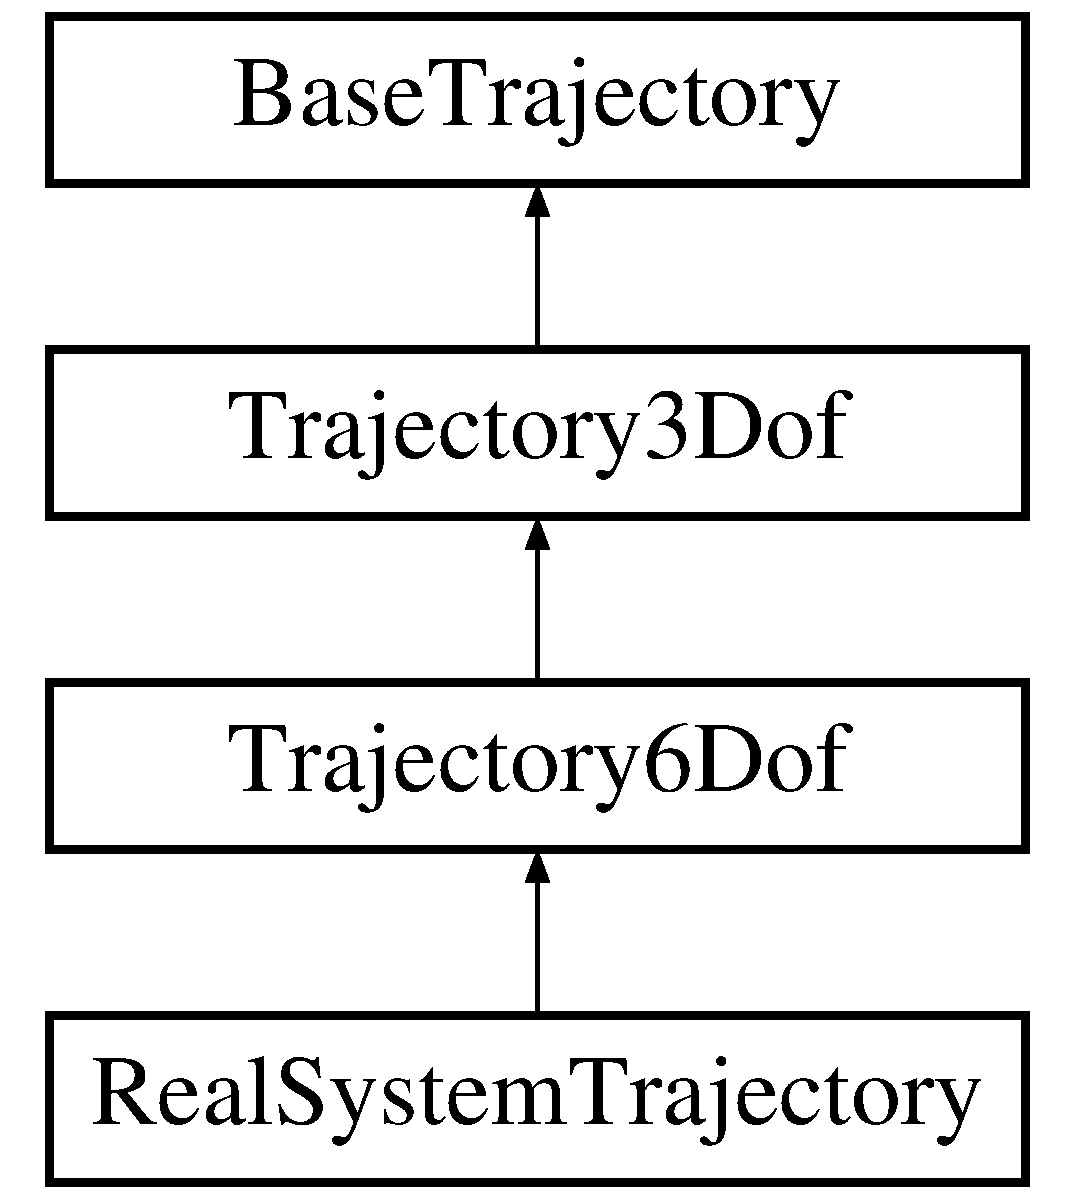
\includegraphics[height=4.000000cm]{class_real_system_trajectory}
\end{center}
\end{figure}
\subsection*{Public Member Functions}
\begin{DoxyCompactItemize}
\item 
\hyperlink{class_real_system_trajectory_acfb42e8dbeadf71ce22d31ed51f0e6c0}{Real\+System\+Trajectory} (Sim\+D\+Preference \&Sim\+Pref)
\begin{DoxyCompactList}\small\item\em constructor \end{DoxyCompactList}\item 
\hyperlink{class_real_system_trajectory_a6ae4a18127c674dd4926ecc7ff92487e}{$\sim$\+Real\+System\+Trajectory} ()
\begin{DoxyCompactList}\small\item\em destructor \end{DoxyCompactList}\item 
void \hyperlink{class_real_system_trajectory_a41ae049eeff69ea6b9daef8027a142a3}{init\+Trajectory} (\hyperlink{group___tools_ga3f1431cb9f76da10f59246d1d743dc2c}{Float64} \&Flight\+Time, Aerodynamic\+Struct \&Aero\+Data, Airframe\+Struct \&Airframe\+Data, Thrust\+Struct \&Thrust\+Data, Aircraft\+Struct \&Aircraft\+Data, Guidance\+Struct \&Guidance\+Data, Navigation\+Struct \&Nav\+Data, Actuator\+Struct \&Actuator\+Data, I\+M\+U\+Struct \&I\+M\+U\+Data)
\begin{DoxyCompactList}\small\item\em initalize trajectory \end{DoxyCompactList}\item 
void \hyperlink{class_real_system_trajectory_a16cace4a95283499ffe59dccabff4c68}{update\+Trajectory} (\hyperlink{group___tools_ga3f1431cb9f76da10f59246d1d743dc2c}{Float64} Flight\+Time, Atmosphere\+Struct \&Atmo\+Data, Aerodynamic\+Struct \&Aero\+Data, Airframe\+Struct \&Airframe\+Data, Thrust\+Struct \&Thrust\+Data, Guidance\+Struct \&Guidance\+Data, Navigation\+Struct \&Nav\+Data, Actuator\+Struct \&Actuator\+Data, I\+M\+U\+Struct \&I\+M\+U\+Data)
\begin{DoxyCompactList}\small\item\em calculate trajectory \end{DoxyCompactList}\item 
void \hyperlink{class_real_system_trajectory_a964468d420db558844a4a3646e99d3b1}{log\+Realsystem\+Trajectory} ()
\begin{DoxyCompactList}\small\item\em log trajectory data \end{DoxyCompactList}\end{DoxyCompactItemize}


\subsection{Detailed Description}
\begin{DoxyAuthor}{Author}
Jan Olucak 
\end{DoxyAuthor}
\begin{DoxyDate}{Date}
28.\+11.\+2017 
\end{DoxyDate}
\begin{DoxyVersion}{Version}
1.\+0
\end{DoxyVersion}
\hyperlink{class_base_trajectory}{Base\+Trajectory} is the superclass for all trajectory classes. 

Definition at line 23 of file Real\+System\+Trajectory.\+h.



\subsection{Constructor \& Destructor Documentation}
\mbox{\Hypertarget{class_real_system_trajectory_acfb42e8dbeadf71ce22d31ed51f0e6c0}\label{class_real_system_trajectory_acfb42e8dbeadf71ce22d31ed51f0e6c0}} 
\index{Real\+System\+Trajectory@{Real\+System\+Trajectory}!Real\+System\+Trajectory@{Real\+System\+Trajectory}}
\index{Real\+System\+Trajectory@{Real\+System\+Trajectory}!Real\+System\+Trajectory@{Real\+System\+Trajectory}}
\subsubsection{\texorpdfstring{Real\+System\+Trajectory()}{RealSystemTrajectory()}}
{\footnotesize\ttfamily Real\+System\+Trajectory\+::\+Real\+System\+Trajectory (\begin{DoxyParamCaption}\item[{Sim\+D\+Preference \&}]{Sim\+Pref }\end{DoxyParamCaption})}



constructor 



Definition at line 3 of file Real\+System\+Trajectory.\+cpp.

\mbox{\Hypertarget{class_real_system_trajectory_a6ae4a18127c674dd4926ecc7ff92487e}\label{class_real_system_trajectory_a6ae4a18127c674dd4926ecc7ff92487e}} 
\index{Real\+System\+Trajectory@{Real\+System\+Trajectory}!````~Real\+System\+Trajectory@{$\sim$\+Real\+System\+Trajectory}}
\index{````~Real\+System\+Trajectory@{$\sim$\+Real\+System\+Trajectory}!Real\+System\+Trajectory@{Real\+System\+Trajectory}}
\subsubsection{\texorpdfstring{$\sim$\+Real\+System\+Trajectory()}{~RealSystemTrajectory()}}
{\footnotesize\ttfamily Real\+System\+Trajectory\+::$\sim$\+Real\+System\+Trajectory (\begin{DoxyParamCaption}{ }\end{DoxyParamCaption})}



destructor 



Definition at line 16 of file Real\+System\+Trajectory.\+cpp.



\subsection{Member Function Documentation}
\mbox{\Hypertarget{class_real_system_trajectory_a41ae049eeff69ea6b9daef8027a142a3}\label{class_real_system_trajectory_a41ae049eeff69ea6b9daef8027a142a3}} 
\index{Real\+System\+Trajectory@{Real\+System\+Trajectory}!init\+Trajectory@{init\+Trajectory}}
\index{init\+Trajectory@{init\+Trajectory}!Real\+System\+Trajectory@{Real\+System\+Trajectory}}
\subsubsection{\texorpdfstring{init\+Trajectory()}{initTrajectory()}}
{\footnotesize\ttfamily void Real\+System\+Trajectory\+::init\+Trajectory (\begin{DoxyParamCaption}\item[{\hyperlink{group___tools_ga3f1431cb9f76da10f59246d1d743dc2c}{Float64} \&}]{Flight\+Time,  }\item[{Aerodynamic\+Struct \&}]{Aero\+Data,  }\item[{Airframe\+Struct \&}]{Airframe\+Data,  }\item[{Thrust\+Struct \&}]{Thrust\+Data,  }\item[{Aircraft\+Struct \&}]{Aircraft\+Data,  }\item[{Guidance\+Struct \&}]{Guidance\+Data,  }\item[{Navigation\+Struct \&}]{Nav\+Data,  }\item[{Actuator\+Struct \&}]{Actuator\+Data,  }\item[{I\+M\+U\+Struct \&}]{I\+M\+U\+Data }\end{DoxyParamCaption})\hspace{0.3cm}{\ttfamily [virtual]}}



initalize trajectory 


\begin{DoxyParams}{Parameters}
{\em Flight\+Time} & flight time \\
\hline
{\em Aero\+Data} & aerodynamic data \\
\hline
{\em Airframe\+Data} & flight states \\
\hline
{\em Thrust\+Data} & thrust forces and moments \\
\hline
{\em Aircraft\+Data} & geometric data of aircraft \\
\hline
{\em Guidance\+Data} & control variables \\
\hline
{\em Nav\+Data} & aircraft position, velocity \\
\hline
{\em Actuator\+Data} & real actuator angles \\
\hline
{\em I\+M\+U\+Data} & measured acceleration \\
\hline
\end{DoxyParams}


Reimplemented from \hyperlink{class_trajectory6_dof_a4e81b667130462a85ce047d4942b794c}{Trajectory6\+Dof}.



Definition at line 20 of file Real\+System\+Trajectory.\+cpp.

\mbox{\Hypertarget{class_real_system_trajectory_a964468d420db558844a4a3646e99d3b1}\label{class_real_system_trajectory_a964468d420db558844a4a3646e99d3b1}} 
\index{Real\+System\+Trajectory@{Real\+System\+Trajectory}!log\+Realsystem\+Trajectory@{log\+Realsystem\+Trajectory}}
\index{log\+Realsystem\+Trajectory@{log\+Realsystem\+Trajectory}!Real\+System\+Trajectory@{Real\+System\+Trajectory}}
\subsubsection{\texorpdfstring{log\+Realsystem\+Trajectory()}{logRealsystemTrajectory()}}
{\footnotesize\ttfamily void Real\+System\+Trajectory\+::log\+Realsystem\+Trajectory (\begin{DoxyParamCaption}{ }\end{DoxyParamCaption})}



log trajectory data 



Definition at line 119 of file Real\+System\+Trajectory.\+cpp.



Referenced by update\+Trajectory().

\mbox{\Hypertarget{class_real_system_trajectory_a16cace4a95283499ffe59dccabff4c68}\label{class_real_system_trajectory_a16cace4a95283499ffe59dccabff4c68}} 
\index{Real\+System\+Trajectory@{Real\+System\+Trajectory}!update\+Trajectory@{update\+Trajectory}}
\index{update\+Trajectory@{update\+Trajectory}!Real\+System\+Trajectory@{Real\+System\+Trajectory}}
\subsubsection{\texorpdfstring{update\+Trajectory()}{updateTrajectory()}}
{\footnotesize\ttfamily void Real\+System\+Trajectory\+::update\+Trajectory (\begin{DoxyParamCaption}\item[{\hyperlink{group___tools_ga3f1431cb9f76da10f59246d1d743dc2c}{Float64}}]{Flight\+Time,  }\item[{Atmosphere\+Struct \&}]{Atmo\+Data,  }\item[{Aerodynamic\+Struct \&}]{Aero\+Data,  }\item[{Airframe\+Struct \&}]{Airframe\+Data,  }\item[{Thrust\+Struct \&}]{Thrust\+Data,  }\item[{Guidance\+Struct \&}]{Guidance\+Data,  }\item[{Navigation\+Struct \&}]{Nav\+Data,  }\item[{Actuator\+Struct \&}]{Actuator\+Data,  }\item[{I\+M\+U\+Struct \&}]{I\+M\+U\+Data }\end{DoxyParamCaption})\hspace{0.3cm}{\ttfamily [virtual]}}



calculate trajectory 


\begin{DoxyParams}{Parameters}
{\em Flight\+Time} & flight time \\
\hline
{\em Atmo\+Data} & current atmospheric data \\
\hline
{\em Aero\+Data} & aerodynamic data \\
\hline
{\em Airframe\+Data} & flight states \\
\hline
{\em Thrust\+Data} & thrust forces and moments \\
\hline
{\em Guidance\+Data} & control variables \\
\hline
{\em Nav\+Data} & aircraft position, velocity \\
\hline
{\em Actuator\+Data} & real actuator angles \\
\hline
{\em I\+M\+U\+Data} & measured acceleration \\
\hline
\end{DoxyParams}


Reimplemented from \hyperlink{class_trajectory6_dof_aafe86c414f4717075a3e0f40c0543fa1}{Trajectory6\+Dof}.



Definition at line 57 of file Real\+System\+Trajectory.\+cpp.



The documentation for this class was generated from the following files\+:\begin{DoxyCompactItemize}
\item 
C\+:/\+Users/janol/\+Desktop/\+Simulation\+\_\+\+Stand230618/\+Trajectory/\hyperlink{_real_system_trajectory_8h}{Real\+System\+Trajectory.\+h}\item 
C\+:/\+Users/janol/\+Desktop/\+Simulation\+\_\+\+Stand230618/\+Trajectory/\hyperlink{_real_system_trajectory_8cpp}{Real\+System\+Trajectory.\+cpp}\end{DoxyCompactItemize}

\hypertarget{class_state_controller}{}\section{State\+Controller Class Reference}
\label{class_state_controller}\index{State\+Controller@{State\+Controller}}
\subsection*{Public Member Functions}
\begin{DoxyCompactItemize}
\item 
\mbox{\Hypertarget{class_state_controller_a179258c5000de44f8a9b2b7dd0e63c68}\label{class_state_controller_a179258c5000de44f8a9b2b7dd0e63c68}} 
void {\bfseries init\+State\+Controller} ()
\item 
\mbox{\Hypertarget{class_state_controller_aec80cee4bc03c82550b28795b275ff9a}\label{class_state_controller_aec80cee4bc03c82550b28795b275ff9a}} 
void {\bfseries update\+State\+Controller} ()
\end{DoxyCompactItemize}


\subsection{Detailed Description}


Definition at line \hyperlink{_state_controller_8h_source_l00006}{6} of file \hyperlink{_state_controller_8h_source}{State\+Controller.\+h}.



The documentation for this class was generated from the following files\+:\begin{DoxyCompactItemize}
\item 
State\+Controller.\+h\item 
State\+Controller.\+cpp\end{DoxyCompactItemize}

\hypertarget{class_thrust_analytical}{}\section{Thrust\+Analytical Class Reference}
\label{class_thrust_analytical}\index{Thrust\+Analytical@{Thrust\+Analytical}}


{\ttfamily \#include $<$Thrust\+Analytical.\+h$>$}

Inheritance diagram for Thrust\+Analytical\+:\begin{figure}[H]
\begin{center}
\leavevmode
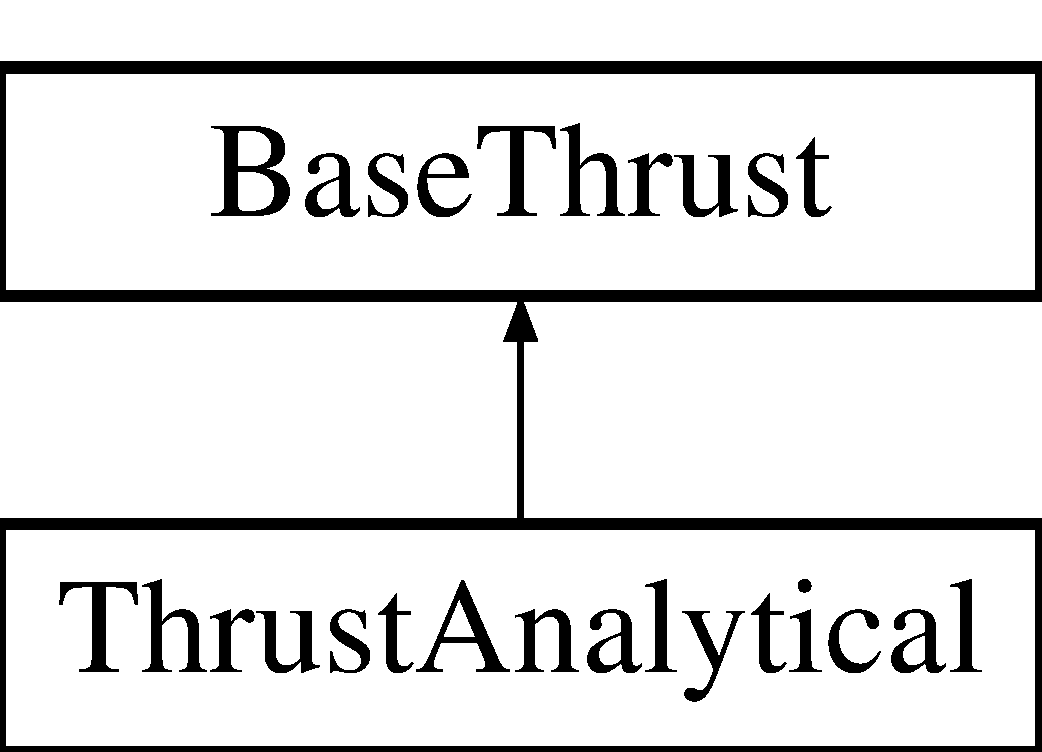
\includegraphics[height=2.000000cm]{class_thrust_analytical}
\end{center}
\end{figure}
\subsection*{Public Member Functions}
\begin{DoxyCompactItemize}
\item 
\hyperlink{class_thrust_analytical_a5c75949a22871e861090560adb2d5f18}{Thrust\+Analytical} ()
\begin{DoxyCompactList}\small\item\em constructor \end{DoxyCompactList}\item 
\hyperlink{class_thrust_analytical_aeaf9dd69c10812c673d6cfae0d7ca4fd}{$\sim$\+Thrust\+Analytical} ()
\begin{DoxyCompactList}\small\item\em destructor \end{DoxyCompactList}\item 
void \hyperlink{class_thrust_analytical_ad6d786911957c0d3105a938ff534600a}{init\+Thrust} (\hyperlink{group___tools_ga3f1431cb9f76da10f59246d1d743dc2c}{Float64} \&Flight\+Time, Thrust\+Struct \&Thrust\+Data, Aircraft\+Struct \&Aircraft\+Data)
\begin{DoxyCompactList}\small\item\em read in Data from Engine.\+dat \end{DoxyCompactList}\item 
void \hyperlink{class_thrust_analytical_a2ef6fcb3ba436e41940573917027b9e5}{update\+Thrust} (\hyperlink{group___tools_ga3f1431cb9f76da10f59246d1d743dc2c}{Float64} Flight\+Time, Atmosphere\+Struct \&Atmo\+Data, Aerodynamic\+Struct \&Aero\+Data, Airframe\+Struct \&Airframe\+Data, Thrust\+Struct \&Thrust\+Data, Actuator\+Struct \&Actuator\+Data)
\item 
void \hyperlink{class_thrust_analytical_ae1b4a04fe4f2a7dd41d6b845e5e36a92}{init\+Log\+Engine\+Data} (\hyperlink{group___tools_ga3f1431cb9f76da10f59246d1d743dc2c}{Float64} \&Flight\+Time, Thrust\+Struct \&Thrust\+Data)
\begin{DoxyCompactList}\small\item\em define output of thrust data \end{DoxyCompactList}\item 
virtual void \hyperlink{class_thrust_analytical_aa3ee59637ce7fb0452195e4d02f400e9}{log\+Engine\+Data} ()
\begin{DoxyCompactList}\small\item\em log engine data \end{DoxyCompactList}\end{DoxyCompactItemize}


\subsection{Detailed Description}
\begin{DoxyAuthor}{Author}
Jan Olucak 
\end{DoxyAuthor}
\begin{DoxyDate}{Date}
25.\+11.\+2017 
\end{DoxyDate}
\begin{DoxyVersion}{Version}
1.\+0
\end{DoxyVersion}
\hyperlink{class_thrust_analytical}{Thrust\+Analytical} class is a child class of \hyperlink{class_base_thrust}{Base\+Thrust} class. Thrust forces and moments are calculated with an analytical model. 

Definition at line 20 of file Thrust\+Analytical.\+h.



\subsection{Constructor \& Destructor Documentation}
\mbox{\Hypertarget{class_thrust_analytical_a5c75949a22871e861090560adb2d5f18}\label{class_thrust_analytical_a5c75949a22871e861090560adb2d5f18}} 
\index{Thrust\+Analytical@{Thrust\+Analytical}!Thrust\+Analytical@{Thrust\+Analytical}}
\index{Thrust\+Analytical@{Thrust\+Analytical}!Thrust\+Analytical@{Thrust\+Analytical}}
\subsubsection{\texorpdfstring{Thrust\+Analytical()}{ThrustAnalytical()}}
{\footnotesize\ttfamily Thrust\+Analytical\+::\+Thrust\+Analytical (\begin{DoxyParamCaption}{ }\end{DoxyParamCaption})}



constructor 



Definition at line 4 of file Thrust\+Analytical.\+cpp.

\mbox{\Hypertarget{class_thrust_analytical_aeaf9dd69c10812c673d6cfae0d7ca4fd}\label{class_thrust_analytical_aeaf9dd69c10812c673d6cfae0d7ca4fd}} 
\index{Thrust\+Analytical@{Thrust\+Analytical}!````~Thrust\+Analytical@{$\sim$\+Thrust\+Analytical}}
\index{````~Thrust\+Analytical@{$\sim$\+Thrust\+Analytical}!Thrust\+Analytical@{Thrust\+Analytical}}
\subsubsection{\texorpdfstring{$\sim$\+Thrust\+Analytical()}{~ThrustAnalytical()}}
{\footnotesize\ttfamily Thrust\+Analytical\+::$\sim$\+Thrust\+Analytical (\begin{DoxyParamCaption}{ }\end{DoxyParamCaption})}



destructor 



Definition at line 12 of file Thrust\+Analytical.\+cpp.



\subsection{Member Function Documentation}
\mbox{\Hypertarget{class_thrust_analytical_ae1b4a04fe4f2a7dd41d6b845e5e36a92}\label{class_thrust_analytical_ae1b4a04fe4f2a7dd41d6b845e5e36a92}} 
\index{Thrust\+Analytical@{Thrust\+Analytical}!init\+Log\+Engine\+Data@{init\+Log\+Engine\+Data}}
\index{init\+Log\+Engine\+Data@{init\+Log\+Engine\+Data}!Thrust\+Analytical@{Thrust\+Analytical}}
\subsubsection{\texorpdfstring{init\+Log\+Engine\+Data()}{initLogEngineData()}}
{\footnotesize\ttfamily void Thrust\+Analytical\+::init\+Log\+Engine\+Data (\begin{DoxyParamCaption}\item[{\hyperlink{group___tools_ga3f1431cb9f76da10f59246d1d743dc2c}{Float64} \&}]{Flight\+Time,  }\item[{Thrust\+Struct \&}]{Thrust\+Data }\end{DoxyParamCaption})}



define output of thrust data 



Definition at line 67 of file Thrust\+Analytical.\+cpp.



Referenced by init\+Thrust().

\mbox{\Hypertarget{class_thrust_analytical_ad6d786911957c0d3105a938ff534600a}\label{class_thrust_analytical_ad6d786911957c0d3105a938ff534600a}} 
\index{Thrust\+Analytical@{Thrust\+Analytical}!init\+Thrust@{init\+Thrust}}
\index{init\+Thrust@{init\+Thrust}!Thrust\+Analytical@{Thrust\+Analytical}}
\subsubsection{\texorpdfstring{init\+Thrust()}{initThrust()}}
{\footnotesize\ttfamily void Thrust\+Analytical\+::init\+Thrust (\begin{DoxyParamCaption}\item[{\hyperlink{group___tools_ga3f1431cb9f76da10f59246d1d743dc2c}{Float64} \&}]{Flight\+Time,  }\item[{Thrust\+Struct \&}]{Thrust\+Data,  }\item[{Aircraft\+Struct \&}]{Aircraft\+Data }\end{DoxyParamCaption})\hspace{0.3cm}{\ttfamily [virtual]}}



read in Data from Engine.\+dat 


\begin{DoxyParams}{Parameters}
{\em Flight\+Time} & flight time \\
\hline
{\em Thrust\+Data} & structure of engine data \\
\hline
{\em Aircraft\+Data} & structure of aircraft data \\
\hline
\end{DoxyParams}
thrust data are read in and variables are initialized 

Reimplemented from \hyperlink{class_base_thrust_a59c4c4eb224cd983c39c8ddc404ad2d6}{Base\+Thrust}.



Definition at line 17 of file Thrust\+Analytical.\+cpp.

\mbox{\Hypertarget{class_thrust_analytical_aa3ee59637ce7fb0452195e4d02f400e9}\label{class_thrust_analytical_aa3ee59637ce7fb0452195e4d02f400e9}} 
\index{Thrust\+Analytical@{Thrust\+Analytical}!log\+Engine\+Data@{log\+Engine\+Data}}
\index{log\+Engine\+Data@{log\+Engine\+Data}!Thrust\+Analytical@{Thrust\+Analytical}}
\subsubsection{\texorpdfstring{log\+Engine\+Data()}{logEngineData()}}
{\footnotesize\ttfamily void Thrust\+Analytical\+::log\+Engine\+Data (\begin{DoxyParamCaption}{ }\end{DoxyParamCaption})\hspace{0.3cm}{\ttfamily [virtual]}}



log engine data 



Reimplemented from \hyperlink{class_base_thrust_af13088a23a8c57cedede6930ee61d52e}{Base\+Thrust}.



Definition at line 78 of file Thrust\+Analytical.\+cpp.

\mbox{\Hypertarget{class_thrust_analytical_a2ef6fcb3ba436e41940573917027b9e5}\label{class_thrust_analytical_a2ef6fcb3ba436e41940573917027b9e5}} 
\index{Thrust\+Analytical@{Thrust\+Analytical}!update\+Thrust@{update\+Thrust}}
\index{update\+Thrust@{update\+Thrust}!Thrust\+Analytical@{Thrust\+Analytical}}
\subsubsection{\texorpdfstring{update\+Thrust()}{updateThrust()}}
{\footnotesize\ttfamily void Thrust\+Analytical\+::update\+Thrust (\begin{DoxyParamCaption}\item[{\hyperlink{group___tools_ga3f1431cb9f76da10f59246d1d743dc2c}{Float64}}]{Flight\+Time,  }\item[{Atmosphere\+Struct \&}]{Atmo\+Data,  }\item[{Aerodynamic\+Struct \&}]{Aero\+Data,  }\item[{Airframe\+Struct \&}]{Airframe\+Data,  }\item[{Thrust\+Struct \&}]{Thrust\+Data,  }\item[{Actuator\+Struct \&}]{Actuator\+Data }\end{DoxyParamCaption})\hspace{0.3cm}{\ttfamily [virtual]}}

The update function from the selected engine is called by a pointer. 
\begin{DoxyParams}{Parameters}
{\em Flight\+Time} & flight time \\
\hline
{\em Atmo\+Data} & get current atmospheric data \\
\hline
{\em Aero\+Data} & get mach number \\
\hline
{\em Airframe\+Data} & get current throttle stick position \\
\hline
{\em Thrust\+Data} & store thrust data \\
\hline
{\em Actuator\+Data} & get thrust stick position \\
\hline
\end{DoxyParams}
1) calculate absolute thrust force

2) calculate thrust force and moments depending on incidence angle and engine position 

Reimplemented from \hyperlink{class_base_thrust_a48a3d47f4b4b40f53f7f86ebf58e4c06}{Base\+Thrust}.



Definition at line 45 of file Thrust\+Analytical.\+cpp.



The documentation for this class was generated from the following files\+:\begin{DoxyCompactItemize}
\item 
C\+:/\+Users/janol/\+Desktop/\+Simulation\+\_\+\+Stand230618/\+Engine/\hyperlink{_thrust_analytical_8h}{Thrust\+Analytical.\+h}\item 
C\+:/\+Users/janol/\+Desktop/\+Simulation\+\_\+\+Stand230618/\+Engine/\hyperlink{_thrust_analytical_8cpp}{Thrust\+Analytical.\+cpp}\end{DoxyCompactItemize}

\hypertarget{class_trajectory}{}\section{Trajectory Class Reference}
\label{class_trajectory}\index{Trajectory@{Trajectory}}


{\ttfamily \#include $<$Trajectory.\+h$>$}

\subsection*{Public Member Functions}
\begin{DoxyCompactItemize}
\item 
\hyperlink{class_trajectory_a8d2001c718f24b178ca0dd84ec1a3960}{Trajectory} (Sim\+D\+Preference \&Sim\+Pref)
\begin{DoxyCompactList}\small\item\em constructor \end{DoxyCompactList}\item 
\hyperlink{class_trajectory_ac673c37025ca5353ad99ab41c936e75d}{$\sim$\+Trajectory} ()
\begin{DoxyCompactList}\small\item\em destructor \end{DoxyCompactList}\item 
void \hyperlink{class_trajectory_a4db29356942a4625c45848eb4e4ae5c8}{select\+Trajectory} (int type, Sim\+D\+Preference \&Sim\+Pref)
\begin{DoxyCompactList}\small\item\em switch function to select desired trajecotry model \end{DoxyCompactList}\item 
void \hyperlink{class_trajectory_acc91a96613419c3f72c43073c3ccda5d}{update\+Trajectory} (\hyperlink{group___tools_ga3f1431cb9f76da10f59246d1d743dc2c}{Float64} Flight\+Time, Atmosphere\+Struct \&Atmo\+Data, Aerodynamic\+Struct \&Aero\+Data, Airframe\+Struct \&Airframe\+Data, Thrust\+Struct \&Thrust\+Data, Guidance\+Struct \&Guidance\+Data, Navigation\+Struct \&Nav\+Data, Actuator\+Struct \&Actuator\+Data, I\+M\+U\+Struct \&I\+M\+U\+Data)
\begin{DoxyCompactList}\small\item\em calculate trajectory \end{DoxyCompactList}\item 
void \hyperlink{class_trajectory_a1cfa48216ff480563708998e3b8dab5f}{init\+Trajectory} (\hyperlink{group___tools_ga3f1431cb9f76da10f59246d1d743dc2c}{Float64} \&Flight\+Time, Aerodynamic\+Struct \&Aero\+Data, Airframe\+Struct \&Airframe\+Data, Thrust\+Struct \&Thrust\+Data, Aircraft\+Struct \&Aircraft\+Data, Guidance\+Struct \&Guidance\+Data, Navigation\+Struct \&Nav\+Data, Actuator\+Struct \&Actuator\+Data, I\+M\+U\+Struct \&I\+M\+U\+Data)
\begin{DoxyCompactList}\small\item\em initalize trajectory \end{DoxyCompactList}\item 
void \hyperlink{class_trajectory_abe592d5604997ea7ed8ce24c1750100f}{log\+Traj} ()
\begin{DoxyCompactList}\small\item\em log trajectory data \end{DoxyCompactList}\end{DoxyCompactItemize}


\subsection{Detailed Description}


Definition at line 18 of file Trajectory.\+h.



\subsection{Constructor \& Destructor Documentation}
\mbox{\Hypertarget{class_trajectory_a8d2001c718f24b178ca0dd84ec1a3960}\label{class_trajectory_a8d2001c718f24b178ca0dd84ec1a3960}} 
\index{Trajectory@{Trajectory}!Trajectory@{Trajectory}}
\index{Trajectory@{Trajectory}!Trajectory@{Trajectory}}
\subsubsection{\texorpdfstring{Trajectory()}{Trajectory()}}
{\footnotesize\ttfamily Trajectory\+::\+Trajectory (\begin{DoxyParamCaption}\item[{Sim\+D\+Preference \&}]{Sim\+Pref }\end{DoxyParamCaption})}



constructor 


\begin{DoxyParams}{Parameters}
{\em Sim\+Pref} & mode selection for trajectory \\
\hline
\end{DoxyParams}


Definition at line 3 of file Trajectory.\+cpp.

\mbox{\Hypertarget{class_trajectory_ac673c37025ca5353ad99ab41c936e75d}\label{class_trajectory_ac673c37025ca5353ad99ab41c936e75d}} 
\index{Trajectory@{Trajectory}!````~Trajectory@{$\sim$\+Trajectory}}
\index{````~Trajectory@{$\sim$\+Trajectory}!Trajectory@{Trajectory}}
\subsubsection{\texorpdfstring{$\sim$\+Trajectory()}{~Trajectory()}}
{\footnotesize\ttfamily Trajectory\+::$\sim$\+Trajectory (\begin{DoxyParamCaption}{ }\end{DoxyParamCaption})}



destructor 



Definition at line 9 of file Trajectory.\+cpp.



\subsection{Member Function Documentation}
\mbox{\Hypertarget{class_trajectory_a1cfa48216ff480563708998e3b8dab5f}\label{class_trajectory_a1cfa48216ff480563708998e3b8dab5f}} 
\index{Trajectory@{Trajectory}!init\+Trajectory@{init\+Trajectory}}
\index{init\+Trajectory@{init\+Trajectory}!Trajectory@{Trajectory}}
\subsubsection{\texorpdfstring{init\+Trajectory()}{initTrajectory()}}
{\footnotesize\ttfamily void Trajectory\+::init\+Trajectory (\begin{DoxyParamCaption}\item[{\hyperlink{group___tools_ga3f1431cb9f76da10f59246d1d743dc2c}{Float64} \&}]{Flight\+Time,  }\item[{Aerodynamic\+Struct \&}]{Aero\+Data,  }\item[{Airframe\+Struct \&}]{Airframe\+Data,  }\item[{Thrust\+Struct \&}]{Thrust\+Data,  }\item[{Aircraft\+Struct \&}]{Aircraft\+Data,  }\item[{Guidance\+Struct \&}]{Guidance\+Data,  }\item[{Navigation\+Struct \&}]{Nav\+Data,  }\item[{Actuator\+Struct \&}]{Actuator\+Data,  }\item[{I\+M\+U\+Struct \&}]{I\+M\+U\+Data }\end{DoxyParamCaption})}



initalize trajectory 


\begin{DoxyParams}{Parameters}
{\em Flight\+Time} & flight time \\
\hline
{\em Aero\+Data} & aerodynamic data \\
\hline
{\em Airframe\+Data} & flight states \\
\hline
{\em Thrust\+Data} & thrust forces and moments \\
\hline
{\em Aircraft\+Data} & geometric data of aircraft \\
\hline
{\em Guidance\+Data} & control variables \\
\hline
{\em Nav\+Data} & aircraft position, velocity \\
\hline
{\em Actuator\+Data} & real actuator angles \\
\hline
{\em I\+M\+U\+Data} & measured acceleration \\
\hline
\end{DoxyParams}


Definition at line 59 of file Trajectory.\+cpp.



Referenced by Aircraft\+::simulate\+Aircraft(), and Trajectory\+Test().

\mbox{\Hypertarget{class_trajectory_abe592d5604997ea7ed8ce24c1750100f}\label{class_trajectory_abe592d5604997ea7ed8ce24c1750100f}} 
\index{Trajectory@{Trajectory}!log\+Traj@{log\+Traj}}
\index{log\+Traj@{log\+Traj}!Trajectory@{Trajectory}}
\subsubsection{\texorpdfstring{log\+Traj()}{logTraj()}}
{\footnotesize\ttfamily void Trajectory\+::log\+Traj (\begin{DoxyParamCaption}{ }\end{DoxyParamCaption})}



log trajectory data 



Definition at line 81 of file Trajectory.\+cpp.

\mbox{\Hypertarget{class_trajectory_a4db29356942a4625c45848eb4e4ae5c8}\label{class_trajectory_a4db29356942a4625c45848eb4e4ae5c8}} 
\index{Trajectory@{Trajectory}!select\+Trajectory@{select\+Trajectory}}
\index{select\+Trajectory@{select\+Trajectory}!Trajectory@{Trajectory}}
\subsubsection{\texorpdfstring{select\+Trajectory()}{selectTrajectory()}}
{\footnotesize\ttfamily void Trajectory\+::select\+Trajectory (\begin{DoxyParamCaption}\item[{int}]{type,  }\item[{Sim\+D\+Preference \&}]{Sim\+Pref }\end{DoxyParamCaption})}



switch function to select desired trajecotry model 


\begin{DoxyParams}{Parameters}
{\em type} & trajectory model \\
\hline
{\em Sim\+Pref} & selection of module models \\
\hline
\end{DoxyParams}


Definition at line 13 of file Trajectory.\+cpp.



Referenced by Trajectory().

\mbox{\Hypertarget{class_trajectory_acc91a96613419c3f72c43073c3ccda5d}\label{class_trajectory_acc91a96613419c3f72c43073c3ccda5d}} 
\index{Trajectory@{Trajectory}!update\+Trajectory@{update\+Trajectory}}
\index{update\+Trajectory@{update\+Trajectory}!Trajectory@{Trajectory}}
\subsubsection{\texorpdfstring{update\+Trajectory()}{updateTrajectory()}}
{\footnotesize\ttfamily void Trajectory\+::update\+Trajectory (\begin{DoxyParamCaption}\item[{\hyperlink{group___tools_ga3f1431cb9f76da10f59246d1d743dc2c}{Float64}}]{Flight\+Time,  }\item[{Atmosphere\+Struct \&}]{Atmo\+Data,  }\item[{Aerodynamic\+Struct \&}]{Aero\+Data,  }\item[{Airframe\+Struct \&}]{Airframe\+Data,  }\item[{Thrust\+Struct \&}]{Thrust\+Data,  }\item[{Guidance\+Struct \&}]{Guidance\+Data,  }\item[{Navigation\+Struct \&}]{Nav\+Data,  }\item[{Actuator\+Struct \&}]{Actuator\+Data,  }\item[{I\+M\+U\+Struct \&}]{I\+M\+U\+Data }\end{DoxyParamCaption})}



calculate trajectory 


\begin{DoxyParams}{Parameters}
{\em Flight\+Time} & flight time \\
\hline
{\em Atmo\+Data} & current atmospheric data \\
\hline
{\em Aero\+Data} & aerodynamic data \\
\hline
{\em Airframe\+Data} & flight states \\
\hline
{\em Thrust\+Data} & thrust forces and moments \\
\hline
{\em Guidance\+Data} & control variables \\
\hline
{\em Nav\+Data} & aircraft position, velocity \\
\hline
{\em Actuator\+Data} & real actuator angles \\
\hline
{\em I\+M\+U\+Data} & measured acceleration \\
\hline
\end{DoxyParams}


Definition at line 38 of file Trajectory.\+cpp.



Referenced by Aircraft\+::simulate\+Aircraft(), and Trajectory\+Test().



The documentation for this class was generated from the following files\+:\begin{DoxyCompactItemize}
\item 
C\+:/\+Users/janol/\+Desktop/\+Simulation\+\_\+\+Stand230618/\+Trajectory/\hyperlink{_trajectory_8h}{Trajectory.\+h}\item 
C\+:/\+Users/janol/\+Desktop/\+Simulation\+\_\+\+Stand230618/\+Trajectory/\hyperlink{_trajectory_8cpp}{Trajectory.\+cpp}\end{DoxyCompactItemize}

\hypertarget{class_trajectory3_dof}{}\section{Trajectory3\+Dof Class Reference}
\label{class_trajectory3_dof}\index{Trajectory3\+Dof@{Trajectory3\+Dof}}


{\ttfamily \#include $<$Trajectory3\+Do\+F.\+h$>$}

Inheritance diagram for Trajectory3\+Dof\+:\begin{figure}[H]
\begin{center}
\leavevmode
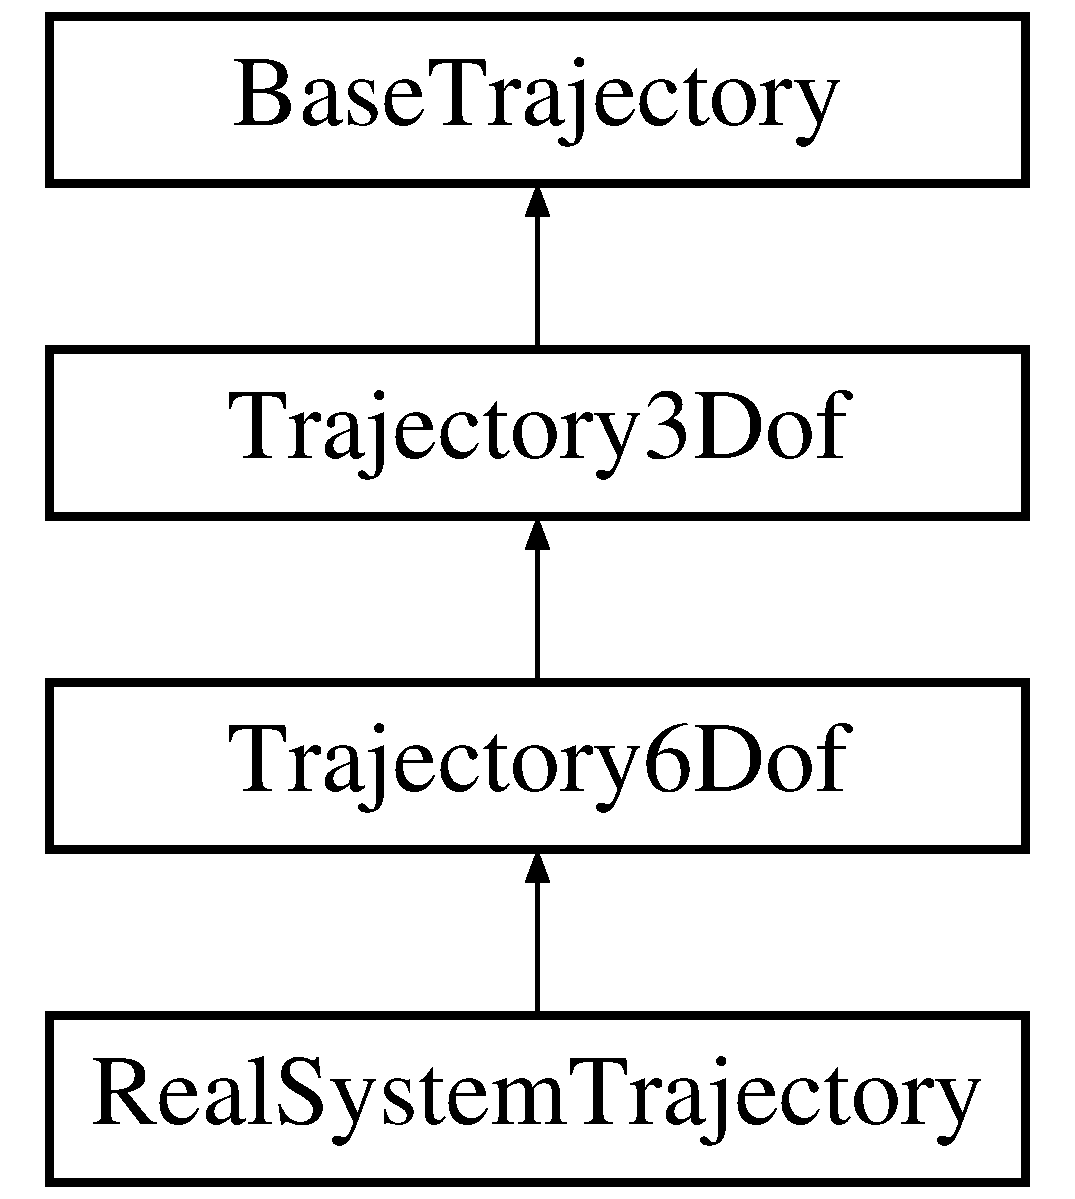
\includegraphics[height=4.000000cm]{class_trajectory3_dof}
\end{center}
\end{figure}
\subsection*{Public Member Functions}
\begin{DoxyCompactItemize}
\item 
\hyperlink{class_trajectory3_dof_a884cf7d2bb8442fb86584385ee35f679}{Trajectory3\+Dof} (Sim\+D\+Preference \&Sim\+Pref)
\begin{DoxyCompactList}\small\item\em constructor \end{DoxyCompactList}\item 
\hyperlink{class_trajectory3_dof_ab7f3c2605332be2030b923e07112e9c2}{$\sim$\+Trajectory3\+Dof} ()
\begin{DoxyCompactList}\small\item\em destructor \end{DoxyCompactList}\item 
virtual void \hyperlink{class_trajectory3_dof_ab132d729efaded8c7942d462d69cba62}{init\+Trajectory} (\hyperlink{group___tools_ga3f1431cb9f76da10f59246d1d743dc2c}{Float64} \&Flight\+Time, Aerodynamic\+Struct \&Aero\+Data, Airframe\+Struct \&Airframe\+Data, Thrust\+Struct \&Thrust\+Data, Aircraft\+Struct \&Aircraft\+Data, Guidance\+Struct \&Guidance\+Data, Navigation\+Struct \&Nav\+Data, Actuator\+Struct \&Actuator\+Data, I\+M\+U\+Struct \&I\+M\+U\+Data)
\begin{DoxyCompactList}\small\item\em initalize trajectory \end{DoxyCompactList}\item 
virtual void \hyperlink{class_trajectory3_dof_a286d578ad75beaf1018350167557a457}{update\+Trajectory} (\hyperlink{group___tools_ga3f1431cb9f76da10f59246d1d743dc2c}{Float64} Flight\+Time, Atmosphere\+Struct \&Atmo\+Data, Aerodynamic\+Struct \&Aero\+Data, Airframe\+Struct \&Airframe\+Data, Thrust\+Struct \&Thrust\+Data, Guidance\+Struct \&Guidance\+Data, Navigation\+Struct \&Nav\+Data, Actuator\+Struct \&Actuator\+Data, I\+M\+U\+Struct \&I\+M\+U\+Data)
\begin{DoxyCompactList}\small\item\em calculate trajectory \end{DoxyCompactList}\item 
void \hyperlink{class_trajectory3_dof_a8a31fd7c0d76f6f158e62b23f2128f86}{init\+Trajectory3\+DoF} (\hyperlink{group___tools_ga3f1431cb9f76da10f59246d1d743dc2c}{Float64} \&Flight\+Time, Aerodynamic\+Struct \&Aero\+Data, Airframe\+Struct \&Airframe\+Data, Thrust\+Struct \&Thrust\+Data, Aircraft\+Struct \&Aircraft\+Data)
\begin{DoxyCompactList}\small\item\em initalize 3 Dof trajectory \end{DoxyCompactList}\item 
void \hyperlink{class_trajectory3_dof_ad3bc8f72bdd7ceed04732de4f0a80926}{update\+Trajectory3\+DoF} (\hyperlink{group___tools_ga3f1431cb9f76da10f59246d1d743dc2c}{Float64} Flight\+Time, Atmosphere\+Struct \&Atmo\+Data, Aerodynamic\+Struct \&Aero\+Data, Airframe\+Struct \&Airframe\+Data, Thrust\+Struct \&Thrust\+Data, Actuator\+Struct \&Actuator\+Data, I\+M\+U\+Struct \&I\+M\+U\+Data, Navigation\+Struct \&Nav\+Data)
\begin{DoxyCompactList}\small\item\em calculate 3 Dof trajectory \end{DoxyCompactList}\item 
void \hyperlink{class_trajectory3_dof_a0ec1ae76ec1d60f03aaef9107b749cd0}{log3\+Dof\+Data} ()
\begin{DoxyCompactList}\small\item\em log 3\+Dof Data (Aerodynamic Data, Thrust Data and translational acclerations) \end{DoxyCompactList}\end{DoxyCompactItemize}


\subsection{Detailed Description}


Definition at line 19 of file Trajectory3\+Do\+F.\+h.



\subsection{Constructor \& Destructor Documentation}
\mbox{\Hypertarget{class_trajectory3_dof_a884cf7d2bb8442fb86584385ee35f679}\label{class_trajectory3_dof_a884cf7d2bb8442fb86584385ee35f679}} 
\index{Trajectory3\+Dof@{Trajectory3\+Dof}!Trajectory3\+Dof@{Trajectory3\+Dof}}
\index{Trajectory3\+Dof@{Trajectory3\+Dof}!Trajectory3\+Dof@{Trajectory3\+Dof}}
\subsubsection{\texorpdfstring{Trajectory3\+Dof()}{Trajectory3Dof()}}
{\footnotesize\ttfamily Trajectory3\+Dof\+::\+Trajectory3\+Dof (\begin{DoxyParamCaption}\item[{Sim\+D\+Preference \&}]{Sim\+Pref }\end{DoxyParamCaption})}



constructor 


\begin{DoxyParams}{Parameters}
{\em Sim\+Pref} & mode selection for trajectory \\
\hline
\end{DoxyParams}


Definition at line 3 of file Trajectory3\+Do\+F.\+cpp.

\mbox{\Hypertarget{class_trajectory3_dof_ab7f3c2605332be2030b923e07112e9c2}\label{class_trajectory3_dof_ab7f3c2605332be2030b923e07112e9c2}} 
\index{Trajectory3\+Dof@{Trajectory3\+Dof}!````~Trajectory3\+Dof@{$\sim$\+Trajectory3\+Dof}}
\index{````~Trajectory3\+Dof@{$\sim$\+Trajectory3\+Dof}!Trajectory3\+Dof@{Trajectory3\+Dof}}
\subsubsection{\texorpdfstring{$\sim$\+Trajectory3\+Dof()}{~Trajectory3Dof()}}
{\footnotesize\ttfamily Trajectory3\+Dof\+::$\sim$\+Trajectory3\+Dof (\begin{DoxyParamCaption}{ }\end{DoxyParamCaption})}



destructor 



Definition at line 11 of file Trajectory3\+Do\+F.\+cpp.



\subsection{Member Function Documentation}
\mbox{\Hypertarget{class_trajectory3_dof_ab132d729efaded8c7942d462d69cba62}\label{class_trajectory3_dof_ab132d729efaded8c7942d462d69cba62}} 
\index{Trajectory3\+Dof@{Trajectory3\+Dof}!init\+Trajectory@{init\+Trajectory}}
\index{init\+Trajectory@{init\+Trajectory}!Trajectory3\+Dof@{Trajectory3\+Dof}}
\subsubsection{\texorpdfstring{init\+Trajectory()}{initTrajectory()}}
{\footnotesize\ttfamily void Trajectory3\+Dof\+::init\+Trajectory (\begin{DoxyParamCaption}\item[{\hyperlink{group___tools_ga3f1431cb9f76da10f59246d1d743dc2c}{Float64} \&}]{Flight\+Time,  }\item[{Aerodynamic\+Struct \&}]{Aero\+Data,  }\item[{Airframe\+Struct \&}]{Airframe\+Data,  }\item[{Thrust\+Struct \&}]{Thrust\+Data,  }\item[{Aircraft\+Struct \&}]{Aircraft\+Data,  }\item[{Guidance\+Struct \&}]{Guidance\+Data,  }\item[{Navigation\+Struct \&}]{Nav\+Data,  }\item[{Actuator\+Struct \&}]{Actuator\+Data,  }\item[{I\+M\+U\+Struct \&}]{I\+M\+U\+Data }\end{DoxyParamCaption})\hspace{0.3cm}{\ttfamily [virtual]}}



initalize trajectory 


\begin{DoxyParams}{Parameters}
{\em Flight\+Time} & flight time \\
\hline
{\em Aero\+Data} & aerodynamic data \\
\hline
{\em Airframe\+Data} & flight states \\
\hline
{\em Thrust\+Data} & thrust forces and moments \\
\hline
{\em Aircraft\+Data} & geometric data of aircraft \\
\hline
{\em Guidance\+Data} & control variables \\
\hline
{\em Nav\+Data} & aircraft position, velocity \\
\hline
{\em Actuator\+Data} & real actuator angles \\
\hline
{\em I\+M\+U\+Data} & measured acceleration \\
\hline
\end{DoxyParams}


Reimplemented from \hyperlink{class_base_trajectory_a4fb09cefd92da44f4e754c8c48f964b5}{Base\+Trajectory}.



Reimplemented in \hyperlink{class_real_system_trajectory_a41ae049eeff69ea6b9daef8027a142a3}{Real\+System\+Trajectory}, and \hyperlink{class_trajectory6_dof_a4e81b667130462a85ce047d4942b794c}{Trajectory6\+Dof}.



Definition at line 15 of file Trajectory3\+Do\+F.\+cpp.

\mbox{\Hypertarget{class_trajectory3_dof_a8a31fd7c0d76f6f158e62b23f2128f86}\label{class_trajectory3_dof_a8a31fd7c0d76f6f158e62b23f2128f86}} 
\index{Trajectory3\+Dof@{Trajectory3\+Dof}!init\+Trajectory3\+DoF@{init\+Trajectory3\+DoF}}
\index{init\+Trajectory3\+DoF@{init\+Trajectory3\+DoF}!Trajectory3\+Dof@{Trajectory3\+Dof}}
\subsubsection{\texorpdfstring{init\+Trajectory3\+Do\+F()}{initTrajectory3DoF()}}
{\footnotesize\ttfamily void Trajectory3\+Dof\+::init\+Trajectory3\+DoF (\begin{DoxyParamCaption}\item[{\hyperlink{group___tools_ga3f1431cb9f76da10f59246d1d743dc2c}{Float64} \&}]{Flight\+Time,  }\item[{Aerodynamic\+Struct \&}]{Aero\+Data,  }\item[{Airframe\+Struct \&}]{Airframe\+Data,  }\item[{Thrust\+Struct \&}]{Thrust\+Data,  }\item[{Aircraft\+Struct \&}]{Aircraft\+Data }\end{DoxyParamCaption})}



initalize 3 Dof trajectory 


\begin{DoxyParams}{Parameters}
{\em Flight\+Time} & flight time \\
\hline
{\em Aero\+Data} & aerodynamic data \\
\hline
{\em Airframe\+Data} & flight states \\
\hline
{\em Thrust\+Data} & thrust forces and moments \\
\hline
{\em Aircraft\+Data} & geometric data of aircraft \\
\hline
\end{DoxyParams}


Definition at line 55 of file Trajectory3\+Do\+F.\+cpp.



Referenced by init\+Trajectory(), Trajectory6\+Dof\+::init\+Trajectory(), and Real\+System\+Trajectory\+::init\+Trajectory().

\mbox{\Hypertarget{class_trajectory3_dof_a0ec1ae76ec1d60f03aaef9107b749cd0}\label{class_trajectory3_dof_a0ec1ae76ec1d60f03aaef9107b749cd0}} 
\index{Trajectory3\+Dof@{Trajectory3\+Dof}!log3\+Dof\+Data@{log3\+Dof\+Data}}
\index{log3\+Dof\+Data@{log3\+Dof\+Data}!Trajectory3\+Dof@{Trajectory3\+Dof}}
\subsubsection{\texorpdfstring{log3\+Dof\+Data()}{log3DofData()}}
{\footnotesize\ttfamily void Trajectory3\+Dof\+::log3\+Dof\+Data (\begin{DoxyParamCaption}{ }\end{DoxyParamCaption})}



log 3\+Dof Data (Aerodynamic Data, Thrust Data and translational acclerations) 



Definition at line 108 of file Trajectory3\+Do\+F.\+cpp.



Referenced by Trajectory6\+Dof\+::log6\+Dof\+Data(), and Real\+System\+Trajectory\+::log\+Realsystem\+Trajectory().

\mbox{\Hypertarget{class_trajectory3_dof_a286d578ad75beaf1018350167557a457}\label{class_trajectory3_dof_a286d578ad75beaf1018350167557a457}} 
\index{Trajectory3\+Dof@{Trajectory3\+Dof}!update\+Trajectory@{update\+Trajectory}}
\index{update\+Trajectory@{update\+Trajectory}!Trajectory3\+Dof@{Trajectory3\+Dof}}
\subsubsection{\texorpdfstring{update\+Trajectory()}{updateTrajectory()}}
{\footnotesize\ttfamily void Trajectory3\+Dof\+::update\+Trajectory (\begin{DoxyParamCaption}\item[{\hyperlink{group___tools_ga3f1431cb9f76da10f59246d1d743dc2c}{Float64}}]{Flight\+Time,  }\item[{Atmosphere\+Struct \&}]{Atmo\+Data,  }\item[{Aerodynamic\+Struct \&}]{Aero\+Data,  }\item[{Airframe\+Struct \&}]{Airframe\+Data,  }\item[{Thrust\+Struct \&}]{Thrust\+Data,  }\item[{Guidance\+Struct \&}]{Guidance\+Data,  }\item[{Navigation\+Struct \&}]{Nav\+Data,  }\item[{Actuator\+Struct \&}]{Actuator\+Data,  }\item[{I\+M\+U\+Struct \&}]{I\+M\+U\+Data }\end{DoxyParamCaption})\hspace{0.3cm}{\ttfamily [virtual]}}



calculate trajectory 


\begin{DoxyParams}{Parameters}
{\em Flight\+Time} & flight time \\
\hline
{\em Atmo\+Data} & current atmospheric data \\
\hline
{\em Aero\+Data} & aerodynamic data \\
\hline
{\em Airframe\+Data} & flight states \\
\hline
{\em Thrust\+Data} & thrust forces and moments \\
\hline
{\em Guidance\+Data} & control variables \\
\hline
{\em Nav\+Data} & aircraft position, velocity \\
\hline
{\em Actuator\+Data} & real actuator angles \\
\hline
{\em I\+M\+U\+Data} & measured acceleration \\
\hline
\end{DoxyParams}


Reimplemented from \hyperlink{class_base_trajectory_a37f0fa46532c754413ee67a846a10624}{Base\+Trajectory}.



Reimplemented in \hyperlink{class_trajectory6_dof_aafe86c414f4717075a3e0f40c0543fa1}{Trajectory6\+Dof}, and \hyperlink{class_real_system_trajectory_a16cace4a95283499ffe59dccabff4c68}{Real\+System\+Trajectory}.



Definition at line 33 of file Trajectory3\+Do\+F.\+cpp.

\mbox{\Hypertarget{class_trajectory3_dof_ad3bc8f72bdd7ceed04732de4f0a80926}\label{class_trajectory3_dof_ad3bc8f72bdd7ceed04732de4f0a80926}} 
\index{Trajectory3\+Dof@{Trajectory3\+Dof}!update\+Trajectory3\+DoF@{update\+Trajectory3\+DoF}}
\index{update\+Trajectory3\+DoF@{update\+Trajectory3\+DoF}!Trajectory3\+Dof@{Trajectory3\+Dof}}
\subsubsection{\texorpdfstring{update\+Trajectory3\+Do\+F()}{updateTrajectory3DoF()}}
{\footnotesize\ttfamily void Trajectory3\+Dof\+::update\+Trajectory3\+DoF (\begin{DoxyParamCaption}\item[{\hyperlink{group___tools_ga3f1431cb9f76da10f59246d1d743dc2c}{Float64}}]{Flight\+Time,  }\item[{Atmosphere\+Struct \&}]{Atmo\+Data,  }\item[{Aerodynamic\+Struct \&}]{Aero\+Data,  }\item[{Airframe\+Struct \&}]{Airframe\+Data,  }\item[{Thrust\+Struct \&}]{Thrust\+Data,  }\item[{Actuator\+Struct \&}]{Actuator\+Data,  }\item[{I\+M\+U\+Struct \&}]{I\+M\+U\+Data,  }\item[{Navigation\+Struct \&}]{Nav\+Data }\end{DoxyParamCaption})}



calculate 3 Dof trajectory 


\begin{DoxyParams}{Parameters}
{\em Flight\+Time} & flight time \\
\hline
{\em Atmo\+Data} & current atmospheric data \\
\hline
{\em Aero\+Data} & aerodynamic data \\
\hline
{\em Airframe\+Data} & flight states \\
\hline
{\em Thrust\+Data} & thrust forces and moments \\
\hline
{\em Actuator\+Data} & real actuator angles \\
\hline
{\em I\+M\+U\+Data} & measured acceleration \\
\hline
{\em Nav\+Data} & aircraft position, velocity \\
\hline
\end{DoxyParams}


Definition at line 75 of file Trajectory3\+Do\+F.\+cpp.



Referenced by update\+Trajectory(), Real\+System\+Trajectory\+::update\+Trajectory(), and Trajectory6\+Dof\+::update\+Trajectory().



The documentation for this class was generated from the following files\+:\begin{DoxyCompactItemize}
\item 
C\+:/\+Users/janol/\+Desktop/\+Simulation\+\_\+\+Stand230618/\+Trajectory/\hyperlink{_trajectory3_do_f_8h}{Trajectory3\+Do\+F.\+h}\item 
C\+:/\+Users/janol/\+Desktop/\+Simulation\+\_\+\+Stand230618/\+Trajectory/\hyperlink{_trajectory3_do_f_8cpp}{Trajectory3\+Do\+F.\+cpp}\end{DoxyCompactItemize}

\hypertarget{class_trajectory6_dof}{}\section{Trajectory6\+Dof Class Reference}
\label{class_trajectory6_dof}\index{Trajectory6\+Dof@{Trajectory6\+Dof}}


{\ttfamily \#include $<$Trajectory6\+Do\+F.\+h$>$}

Inheritance diagram for Trajectory6\+Dof\+:\begin{figure}[H]
\begin{center}
\leavevmode
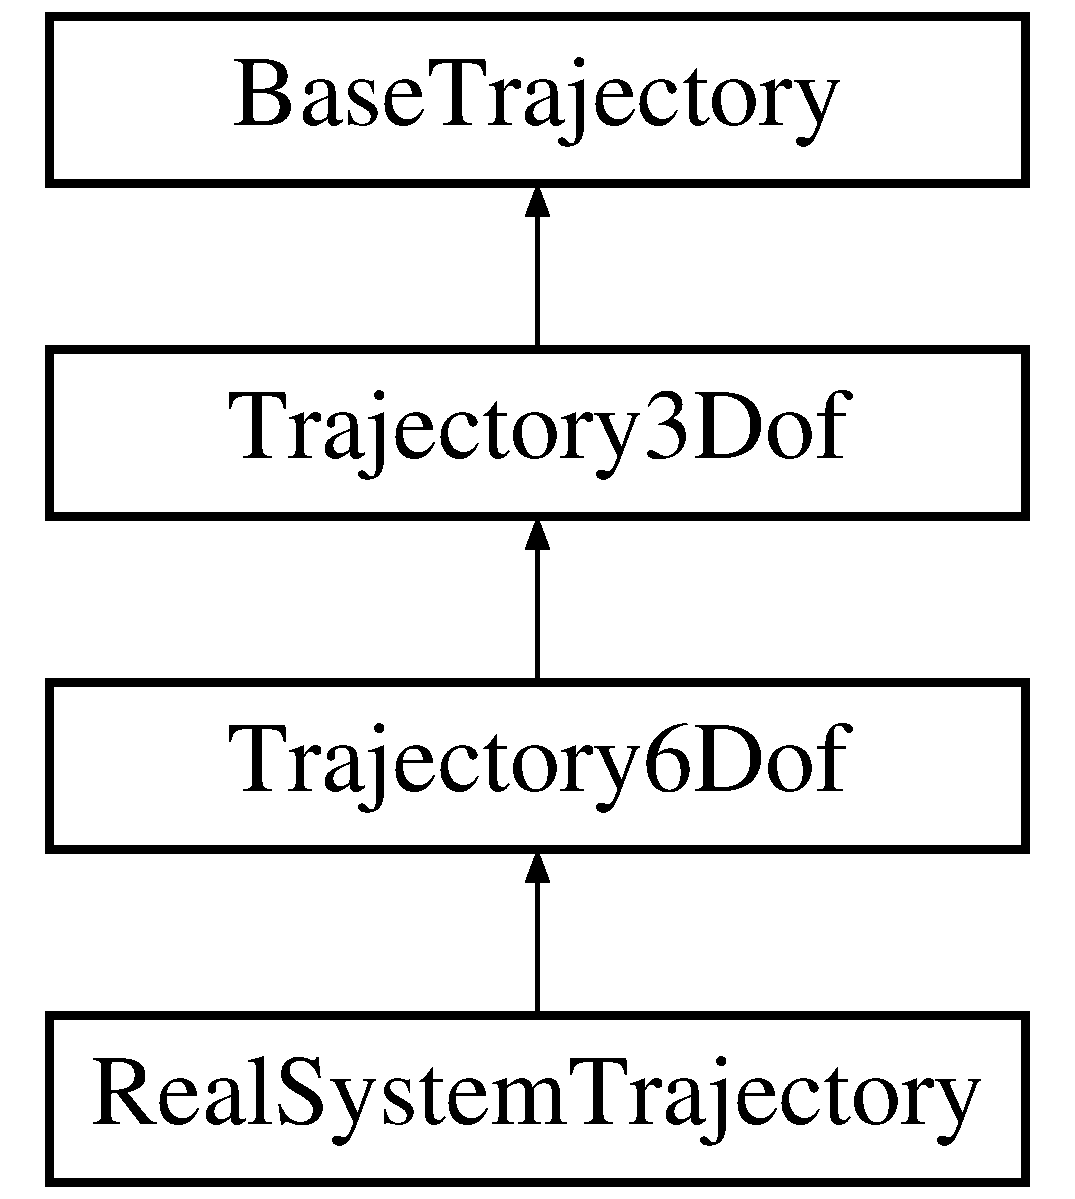
\includegraphics[height=4.000000cm]{class_trajectory6_dof}
\end{center}
\end{figure}
\subsection*{Public Member Functions}
\begin{DoxyCompactItemize}
\item 
\hyperlink{class_trajectory6_dof_a1742bd5d7245f2bd1fb7fadf0ba23e0a}{Trajectory6\+Dof} (Sim\+D\+Preference \&Sim\+Pref)
\begin{DoxyCompactList}\small\item\em constructor \end{DoxyCompactList}\item 
\hyperlink{class_trajectory6_dof_a6bccf2060b63851fcc039ca1efb6f378}{$\sim$\+Trajectory6\+Dof} ()
\begin{DoxyCompactList}\small\item\em destructor \end{DoxyCompactList}\item 
virtual void \hyperlink{class_trajectory6_dof_a4e81b667130462a85ce047d4942b794c}{init\+Trajectory} (\hyperlink{group___tools_ga3f1431cb9f76da10f59246d1d743dc2c}{Float64} \&Flight\+Time, Aerodynamic\+Struct \&Aero\+Data, Airframe\+Struct \&Airframe\+Data, Thrust\+Struct \&Thrust\+Data, Aircraft\+Struct \&Aircraft\+Data, Guidance\+Struct \&Guidance\+Data, Navigation\+Struct \&Nav\+Data, Actuator\+Struct \&Actuator\+Data, I\+M\+U\+Struct \&I\+M\+U\+Data)
\begin{DoxyCompactList}\small\item\em initalize trajectory \end{DoxyCompactList}\item 
virtual void \hyperlink{class_trajectory6_dof_aafe86c414f4717075a3e0f40c0543fa1}{update\+Trajectory} (\hyperlink{group___tools_ga3f1431cb9f76da10f59246d1d743dc2c}{Float64} Flight\+Time, Atmosphere\+Struct \&Atmo\+Data, Aerodynamic\+Struct \&Aero\+Data, Airframe\+Struct \&Airframe\+Data, Thrust\+Struct \&Thrust\+Data, Guidance\+Struct \&Guidance\+Data, Navigation\+Struct \&Nav\+Data, Actuator\+Struct \&Actuator\+Data, I\+M\+U\+Struct \&I\+M\+U\+Data)
\begin{DoxyCompactList}\small\item\em calculate trajectory \end{DoxyCompactList}\item 
void \hyperlink{class_trajectory6_dof_a9ea303538f87c8043058c19b7f981839}{integration\+Trajectory} (Airframe\+Struct \&Airframe\+Data, I\+M\+U\+Struct \&I\+M\+U\+Data, Navigation\+Struct \&Nav\+Data)
\begin{DoxyCompactList}\small\item\em integrate accelerations and calculate new flight states \end{DoxyCompactList}\item 
void \hyperlink{class_trajectory6_dof_aba4e6960a6cec1decfb7f887ddc55c26}{log6\+Dof\+Data} ()
\begin{DoxyCompactList}\small\item\em log 6\+Dof \hyperlink{class_trajectory}{Trajectory} data \end{DoxyCompactList}\item 
void \hyperlink{class_trajectory6_dof_ad0695ba90c621c01a6abc0da03fd8329}{init\+Log6\+Dof} (\hyperlink{group___tools_ga3f1431cb9f76da10f59246d1d743dc2c}{Float64} \&Flight\+Time, I\+M\+U\+Struct \&I\+M\+U\+Data, Navigation\+Struct \&Nav\+Data, Actuator\+Struct \&Actuator\+Data)
\begin{DoxyCompactList}\small\item\em define output for trajectory 6\+D0f \end{DoxyCompactList}\end{DoxyCompactItemize}


\subsection{Detailed Description}


Definition at line 23 of file Trajectory6\+Do\+F.\+h.



\subsection{Constructor \& Destructor Documentation}
\mbox{\Hypertarget{class_trajectory6_dof_a1742bd5d7245f2bd1fb7fadf0ba23e0a}\label{class_trajectory6_dof_a1742bd5d7245f2bd1fb7fadf0ba23e0a}} 
\index{Trajectory6\+Dof@{Trajectory6\+Dof}!Trajectory6\+Dof@{Trajectory6\+Dof}}
\index{Trajectory6\+Dof@{Trajectory6\+Dof}!Trajectory6\+Dof@{Trajectory6\+Dof}}
\subsubsection{\texorpdfstring{Trajectory6\+Dof()}{Trajectory6Dof()}}
{\footnotesize\ttfamily Trajectory6\+Dof\+::\+Trajectory6\+Dof (\begin{DoxyParamCaption}\item[{Sim\+D\+Preference \&}]{Sim\+Pref }\end{DoxyParamCaption})}



constructor 


\begin{DoxyParams}{Parameters}
{\em Sim\+Pref} & mode selection for trajectory \\
\hline
\end{DoxyParams}


Definition at line 3 of file Trajectory6\+Do\+F.\+cpp.

\mbox{\Hypertarget{class_trajectory6_dof_a6bccf2060b63851fcc039ca1efb6f378}\label{class_trajectory6_dof_a6bccf2060b63851fcc039ca1efb6f378}} 
\index{Trajectory6\+Dof@{Trajectory6\+Dof}!````~Trajectory6\+Dof@{$\sim$\+Trajectory6\+Dof}}
\index{````~Trajectory6\+Dof@{$\sim$\+Trajectory6\+Dof}!Trajectory6\+Dof@{Trajectory6\+Dof}}
\subsubsection{\texorpdfstring{$\sim$\+Trajectory6\+Dof()}{~Trajectory6Dof()}}
{\footnotesize\ttfamily Trajectory6\+Dof\+::$\sim$\+Trajectory6\+Dof (\begin{DoxyParamCaption}{ }\end{DoxyParamCaption})}



destructor 



Definition at line 18 of file Trajectory6\+Do\+F.\+cpp.



\subsection{Member Function Documentation}
\mbox{\Hypertarget{class_trajectory6_dof_ad0695ba90c621c01a6abc0da03fd8329}\label{class_trajectory6_dof_ad0695ba90c621c01a6abc0da03fd8329}} 
\index{Trajectory6\+Dof@{Trajectory6\+Dof}!init\+Log6\+Dof@{init\+Log6\+Dof}}
\index{init\+Log6\+Dof@{init\+Log6\+Dof}!Trajectory6\+Dof@{Trajectory6\+Dof}}
\subsubsection{\texorpdfstring{init\+Log6\+Dof()}{initLog6Dof()}}
{\footnotesize\ttfamily void Trajectory6\+Dof\+::init\+Log6\+Dof (\begin{DoxyParamCaption}\item[{\hyperlink{group___tools_ga3f1431cb9f76da10f59246d1d743dc2c}{Float64} \&}]{Flight\+Time,  }\item[{I\+M\+U\+Struct \&}]{I\+M\+U\+Data,  }\item[{Navigation\+Struct \&}]{Nav\+Data,  }\item[{Actuator\+Struct \&}]{Actuator\+Data }\end{DoxyParamCaption})}



define output for trajectory 6\+D0f 


\begin{DoxyParams}{Parameters}
{\em Flight\+Time} & flighttime \\
\hline
{\em I\+M\+U\+Data} & accelerations and rotatory rates \\
\hline
{\em Nav\+Data} & structure that stores position and velocity \\
\hline
{\em Actuator\+Data} & aircraft control deflections \\
\hline
\end{DoxyParams}


Definition at line 142 of file Trajectory6\+Do\+F.\+cpp.



Referenced by init\+Trajectory().

\mbox{\Hypertarget{class_trajectory6_dof_a4e81b667130462a85ce047d4942b794c}\label{class_trajectory6_dof_a4e81b667130462a85ce047d4942b794c}} 
\index{Trajectory6\+Dof@{Trajectory6\+Dof}!init\+Trajectory@{init\+Trajectory}}
\index{init\+Trajectory@{init\+Trajectory}!Trajectory6\+Dof@{Trajectory6\+Dof}}
\subsubsection{\texorpdfstring{init\+Trajectory()}{initTrajectory()}}
{\footnotesize\ttfamily void Trajectory6\+Dof\+::init\+Trajectory (\begin{DoxyParamCaption}\item[{\hyperlink{group___tools_ga3f1431cb9f76da10f59246d1d743dc2c}{Float64} \&}]{Flight\+Time,  }\item[{Aerodynamic\+Struct \&}]{Aero\+Data,  }\item[{Airframe\+Struct \&}]{Airframe\+Data,  }\item[{Thrust\+Struct \&}]{Thrust\+Data,  }\item[{Aircraft\+Struct \&}]{Aircraft\+Data,  }\item[{Guidance\+Struct \&}]{Guidance\+Data,  }\item[{Navigation\+Struct \&}]{Nav\+Data,  }\item[{Actuator\+Struct \&}]{Actuator\+Data,  }\item[{I\+M\+U\+Struct \&}]{I\+M\+U\+Data }\end{DoxyParamCaption})\hspace{0.3cm}{\ttfamily [virtual]}}



initalize trajectory 


\begin{DoxyParams}{Parameters}
{\em Flight\+Time} & flight time \\
\hline
{\em Aero\+Data} & aerodynamic data \\
\hline
{\em Airframe\+Data} & flight states \\
\hline
{\em Thrust\+Data} & thrust forces and moments \\
\hline
{\em Aircraft\+Data} & geometric data of aircraft \\
\hline
{\em Guidance\+Data} & control variables \\
\hline
{\em Nav\+Data} & aircraft position, velocity \\
\hline
{\em Actuator\+Data} & real actuator angles \\
\hline
{\em I\+M\+U\+Data} & measured acceleration \\
\hline
\end{DoxyParams}


Reimplemented from \hyperlink{class_trajectory3_dof_ab132d729efaded8c7942d462d69cba62}{Trajectory3\+Dof}.



Reimplemented in \hyperlink{class_real_system_trajectory_a41ae049eeff69ea6b9daef8027a142a3}{Real\+System\+Trajectory}.



Definition at line 23 of file Trajectory6\+Do\+F.\+cpp.

\mbox{\Hypertarget{class_trajectory6_dof_a9ea303538f87c8043058c19b7f981839}\label{class_trajectory6_dof_a9ea303538f87c8043058c19b7f981839}} 
\index{Trajectory6\+Dof@{Trajectory6\+Dof}!integration\+Trajectory@{integration\+Trajectory}}
\index{integration\+Trajectory@{integration\+Trajectory}!Trajectory6\+Dof@{Trajectory6\+Dof}}
\subsubsection{\texorpdfstring{integration\+Trajectory()}{integrationTrajectory()}}
{\footnotesize\ttfamily void Trajectory6\+Dof\+::integration\+Trajectory (\begin{DoxyParamCaption}\item[{Airframe\+Struct \&}]{Airframe\+Data,  }\item[{I\+M\+U\+Struct \&}]{I\+M\+U\+Data,  }\item[{Navigation\+Struct \&}]{Nav\+Data }\end{DoxyParamCaption})}



integrate accelerations and calculate new flight states 


\begin{DoxyParams}{Parameters}
{\em Airframe\+Data} & flight statess \\
\hline
{\em I\+M\+U\+Data} & accelerations and rotatory rates \\
\hline
{\em Nav\+Data} & structure that stores position and velocity \\
\hline
\end{DoxyParams}


Definition at line 102 of file Trajectory6\+Do\+F.\+cpp.



Referenced by update\+Trajectory().

\mbox{\Hypertarget{class_trajectory6_dof_aba4e6960a6cec1decfb7f887ddc55c26}\label{class_trajectory6_dof_aba4e6960a6cec1decfb7f887ddc55c26}} 
\index{Trajectory6\+Dof@{Trajectory6\+Dof}!log6\+Dof\+Data@{log6\+Dof\+Data}}
\index{log6\+Dof\+Data@{log6\+Dof\+Data}!Trajectory6\+Dof@{Trajectory6\+Dof}}
\subsubsection{\texorpdfstring{log6\+Dof\+Data()}{log6DofData()}}
{\footnotesize\ttfamily void Trajectory6\+Dof\+::log6\+Dof\+Data (\begin{DoxyParamCaption}{ }\end{DoxyParamCaption})}



log 6\+Dof \hyperlink{class_trajectory}{Trajectory} data 



Definition at line 129 of file Trajectory6\+Do\+F.\+cpp.



Referenced by update\+Trajectory().

\mbox{\Hypertarget{class_trajectory6_dof_aafe86c414f4717075a3e0f40c0543fa1}\label{class_trajectory6_dof_aafe86c414f4717075a3e0f40c0543fa1}} 
\index{Trajectory6\+Dof@{Trajectory6\+Dof}!update\+Trajectory@{update\+Trajectory}}
\index{update\+Trajectory@{update\+Trajectory}!Trajectory6\+Dof@{Trajectory6\+Dof}}
\subsubsection{\texorpdfstring{update\+Trajectory()}{updateTrajectory()}}
{\footnotesize\ttfamily void Trajectory6\+Dof\+::update\+Trajectory (\begin{DoxyParamCaption}\item[{\hyperlink{group___tools_ga3f1431cb9f76da10f59246d1d743dc2c}{Float64}}]{Flight\+Time,  }\item[{Atmosphere\+Struct \&}]{Atmo\+Data,  }\item[{Aerodynamic\+Struct \&}]{Aero\+Data,  }\item[{Airframe\+Struct \&}]{Airframe\+Data,  }\item[{Thrust\+Struct \&}]{Thrust\+Data,  }\item[{Guidance\+Struct \&}]{Guidance\+Data,  }\item[{Navigation\+Struct \&}]{Nav\+Data,  }\item[{Actuator\+Struct \&}]{Actuator\+Data,  }\item[{I\+M\+U\+Struct \&}]{I\+M\+U\+Data }\end{DoxyParamCaption})\hspace{0.3cm}{\ttfamily [virtual]}}



calculate trajectory 


\begin{DoxyParams}{Parameters}
{\em Flight\+Time} & flight time \\
\hline
{\em Atmo\+Data} & current atmospheric data \\
\hline
{\em Aero\+Data} & aerodynamic data \\
\hline
{\em Airframe\+Data} & flight states \\
\hline
{\em Thrust\+Data} & thrust forces and moments \\
\hline
{\em Guidance\+Data} & control variables \\
\hline
{\em Nav\+Data} & aircraft position, velocity \\
\hline
{\em Actuator\+Data} & real actuator angles \\
\hline
{\em I\+M\+U\+Data} & measured acceleration \\
\hline
\end{DoxyParams}


Reimplemented from \hyperlink{class_trajectory3_dof_a286d578ad75beaf1018350167557a457}{Trajectory3\+Dof}.



Reimplemented in \hyperlink{class_real_system_trajectory_a16cace4a95283499ffe59dccabff4c68}{Real\+System\+Trajectory}.



Definition at line 55 of file Trajectory6\+Do\+F.\+cpp.



The documentation for this class was generated from the following files\+:\begin{DoxyCompactItemize}
\item 
C\+:/\+Users/janol/\+Desktop/\+Simulation\+\_\+\+Stand230618/\+Trajectory/\hyperlink{_trajectory6_do_f_8h}{Trajectory6\+Do\+F.\+h}\item 
C\+:/\+Users/janol/\+Desktop/\+Simulation\+\_\+\+Stand230618/\+Trajectory/\hyperlink{_trajectory6_do_f_8cpp}{Trajectory6\+Do\+F.\+cpp}\end{DoxyCompactItemize}

\hypertarget{class_transformation}{}\section{Transformation Class Reference}
\label{class_transformation}\index{Transformation@{Transformation}}


{\ttfamily \#include $<$Transformation.\+h$>$}

\subsection*{Public Member Functions}
\begin{DoxyCompactItemize}
\item 
\hyperlink{class_transformation_a40ab64d41c752804740e972ef5f2479f}{Transformation} ()
\begin{DoxyCompactList}\small\item\em constructor \end{DoxyCompactList}\item 
\hyperlink{class_transformation_ade11a9f133b2acd81ae9383187cc255e}{$\sim$\+Transformation} ()
\begin{DoxyCompactList}\small\item\em destructor \end{DoxyCompactList}\item 
Eigen\+::\+Matrix3d \hyperlink{class_transformation_ab33befedbf4f290a0c03367a7fb23e6e}{Mat\+Ned\+To\+Body} (\hyperlink{group___tools_ga3f1431cb9f76da10f59246d1d743dc2c}{Float64} phi, \hyperlink{group___tools_ga3f1431cb9f76da10f59246d1d743dc2c}{Float64} theta, \hyperlink{group___tools_ga3f1431cb9f76da10f59246d1d743dc2c}{Float64} psi)
\begin{DoxyCompactList}\small\item\em tranformation matrix from N\+ED system to body fixed system \end{DoxyCompactList}\item 
Eigen\+::\+Matrix3d \hyperlink{class_transformation_a2c16407225610227ee0c9d2fd2242a29}{Mat\+Body\+To\+N\+ED} (Eigen\+::\+Matrix3d \hyperlink{class_transformation_ab33befedbf4f290a0c03367a7fb23e6e}{Mat\+Ned\+To\+Body})
\begin{DoxyCompactList}\small\item\em tranformation matrix from Body system to N\+ED system \end{DoxyCompactList}\item 
Eigen\+::\+Matrix3d \hyperlink{class_transformation_aaab0c8669b3addd4fc04cd69640c14ec}{Mat\+N\+E\+D\+To\+Trajectory} (\hyperlink{group___tools_ga3f1431cb9f76da10f59246d1d743dc2c}{Float64} Gamma, \hyperlink{group___tools_ga3f1431cb9f76da10f59246d1d743dc2c}{Float64} chi)
\begin{DoxyCompactList}\small\item\em tranformation matrix from N\+ED system to trajectory system \end{DoxyCompactList}\item 
Eigen\+::\+Matrix3d \hyperlink{class_transformation_a9a1ea1611b6e3403ef1f522caf332226}{Mat\+Aero\+To\+Body} (\hyperlink{group___tools_ga3f1431cb9f76da10f59246d1d743dc2c}{Float64} Alpha, \hyperlink{group___tools_ga3f1431cb9f76da10f59246d1d743dc2c}{Float64} Beta)
\begin{DoxyCompactList}\small\item\em tranformation matrix from aerodynamic system to body fixed system \end{DoxyCompactList}\end{DoxyCompactItemize}


\subsection{Detailed Description}
\begin{DoxyAuthor}{Author}
Jan Olucak 
\end{DoxyAuthor}
\begin{DoxyDate}{Date}
25.\+11.\+2017 
\end{DoxyDate}
\begin{DoxyVersion}{Version}
1.\+0
\end{DoxyVersion}
\hyperlink{class_transformation}{Transformation} class provides transformation matrices for flightmechanical coordinate sytems 

Definition at line 19 of file Transformation.\+h.



\subsection{Constructor \& Destructor Documentation}
\mbox{\Hypertarget{class_transformation_a40ab64d41c752804740e972ef5f2479f}\label{class_transformation_a40ab64d41c752804740e972ef5f2479f}} 
\index{Transformation@{Transformation}!Transformation@{Transformation}}
\index{Transformation@{Transformation}!Transformation@{Transformation}}
\subsubsection{\texorpdfstring{Transformation()}{Transformation()}}
{\footnotesize\ttfamily Transformation\+::\+Transformation (\begin{DoxyParamCaption}{ }\end{DoxyParamCaption})}



constructor 



Definition at line 3 of file Transformation.\+cpp.

\mbox{\Hypertarget{class_transformation_ade11a9f133b2acd81ae9383187cc255e}\label{class_transformation_ade11a9f133b2acd81ae9383187cc255e}} 
\index{Transformation@{Transformation}!````~Transformation@{$\sim$\+Transformation}}
\index{````~Transformation@{$\sim$\+Transformation}!Transformation@{Transformation}}
\subsubsection{\texorpdfstring{$\sim$\+Transformation()}{~Transformation()}}
{\footnotesize\ttfamily Transformation\+::$\sim$\+Transformation (\begin{DoxyParamCaption}{ }\end{DoxyParamCaption})}



destructor 



Definition at line 7 of file Transformation.\+cpp.



\subsection{Member Function Documentation}
\mbox{\Hypertarget{class_transformation_a9a1ea1611b6e3403ef1f522caf332226}\label{class_transformation_a9a1ea1611b6e3403ef1f522caf332226}} 
\index{Transformation@{Transformation}!Mat\+Aero\+To\+Body@{Mat\+Aero\+To\+Body}}
\index{Mat\+Aero\+To\+Body@{Mat\+Aero\+To\+Body}!Transformation@{Transformation}}
\subsubsection{\texorpdfstring{Mat\+Aero\+To\+Body()}{MatAeroToBody()}}
{\footnotesize\ttfamily Eigen\+::\+Matrix3d Transformation\+::\+Mat\+Aero\+To\+Body (\begin{DoxyParamCaption}\item[{\hyperlink{group___tools_ga3f1431cb9f76da10f59246d1d743dc2c}{Float64}}]{Alpha,  }\item[{\hyperlink{group___tools_ga3f1431cb9f76da10f59246d1d743dc2c}{Float64}}]{Beta }\end{DoxyParamCaption})}



tranformation matrix from aerodynamic system to body fixed system 


\begin{DoxyParams}{Parameters}
{\em Alpha} & angle of attack \\
\hline
{\em Beta} & angle of sideslip \\
\hline
\end{DoxyParams}


Definition at line 38 of file Transformation.\+cpp.



Referenced by Aerodynamic\+Test(), and Unit\+Test1\+::\+T\+E\+S\+T\+\_\+\+C\+L\+A\+S\+S().

\mbox{\Hypertarget{class_transformation_a2c16407225610227ee0c9d2fd2242a29}\label{class_transformation_a2c16407225610227ee0c9d2fd2242a29}} 
\index{Transformation@{Transformation}!Mat\+Body\+To\+N\+ED@{Mat\+Body\+To\+N\+ED}}
\index{Mat\+Body\+To\+N\+ED@{Mat\+Body\+To\+N\+ED}!Transformation@{Transformation}}
\subsubsection{\texorpdfstring{Mat\+Body\+To\+N\+E\+D()}{MatBodyToNED()}}
{\footnotesize\ttfamily Eigen\+::\+Matrix3d Transformation\+::\+Mat\+Body\+To\+N\+ED (\begin{DoxyParamCaption}\item[{Eigen\+::\+Matrix3d}]{Mat\+Ned\+To\+Body }\end{DoxyParamCaption})}



tranformation matrix from Body system to N\+ED system 


\begin{DoxyParams}{Parameters}
{\em Mat\+Ned\+To\+Body} & invers matrix \\
\hline
\end{DoxyParams}


Definition at line 20 of file Transformation.\+cpp.



Referenced by Trajectory6\+Dof\+::integration\+Trajectory(), and flawless\+Navigation\+::update\+Navigation().

\mbox{\Hypertarget{class_transformation_ab33befedbf4f290a0c03367a7fb23e6e}\label{class_transformation_ab33befedbf4f290a0c03367a7fb23e6e}} 
\index{Transformation@{Transformation}!Mat\+Ned\+To\+Body@{Mat\+Ned\+To\+Body}}
\index{Mat\+Ned\+To\+Body@{Mat\+Ned\+To\+Body}!Transformation@{Transformation}}
\subsubsection{\texorpdfstring{Mat\+Ned\+To\+Body()}{MatNedToBody()}}
{\footnotesize\ttfamily Eigen\+::\+Matrix3d Transformation\+::\+Mat\+Ned\+To\+Body (\begin{DoxyParamCaption}\item[{\hyperlink{group___tools_ga3f1431cb9f76da10f59246d1d743dc2c}{Float64}}]{phi,  }\item[{\hyperlink{group___tools_ga3f1431cb9f76da10f59246d1d743dc2c}{Float64}}]{theta,  }\item[{\hyperlink{group___tools_ga3f1431cb9f76da10f59246d1d743dc2c}{Float64}}]{psi }\end{DoxyParamCaption})}



tranformation matrix from N\+ED system to body fixed system 


\begin{DoxyParams}{Parameters}
{\em phi} & roll angle \\
\hline
{\em theta} & pitch angle \\
\hline
{\em psi} & heading angle \\
\hline
\end{DoxyParams}


Definition at line 11 of file Transformation.\+cpp.



Referenced by Aerodynamic\+Test(), Guidance\+Test(), Trajectory6\+Dof\+::integration\+Trajectory(), Unit\+Test1\+::\+T\+E\+S\+T\+\_\+\+C\+L\+A\+S\+S(), and flawless\+Navigation\+::update\+Navigation().

\mbox{\Hypertarget{class_transformation_aaab0c8669b3addd4fc04cd69640c14ec}\label{class_transformation_aaab0c8669b3addd4fc04cd69640c14ec}} 
\index{Transformation@{Transformation}!Mat\+N\+E\+D\+To\+Trajectory@{Mat\+N\+E\+D\+To\+Trajectory}}
\index{Mat\+N\+E\+D\+To\+Trajectory@{Mat\+N\+E\+D\+To\+Trajectory}!Transformation@{Transformation}}
\subsubsection{\texorpdfstring{Mat\+N\+E\+D\+To\+Trajectory()}{MatNEDToTrajectory()}}
{\footnotesize\ttfamily Eigen\+::\+Matrix3d Transformation\+::\+Mat\+N\+E\+D\+To\+Trajectory (\begin{DoxyParamCaption}\item[{\hyperlink{group___tools_ga3f1431cb9f76da10f59246d1d743dc2c}{Float64}}]{Gamma,  }\item[{\hyperlink{group___tools_ga3f1431cb9f76da10f59246d1d743dc2c}{Float64}}]{chi }\end{DoxyParamCaption})}



tranformation matrix from N\+ED system to trajectory system 


\begin{DoxyParams}{Parameters}
{\em Gamma} & \\
\hline
{\em chi} & azimuth \\
\hline
\end{DoxyParams}


Definition at line 27 of file Transformation.\+cpp.



Referenced by Guidance\+Test(), Trajectory6\+Dof\+::integration\+Trajectory(), Unit\+Test1\+::\+T\+E\+S\+T\+\_\+\+C\+L\+A\+S\+S(), and flawless\+Navigation\+::update\+Navigation().



The documentation for this class was generated from the following files\+:\begin{DoxyCompactItemize}
\item 
C\+:/\+Users/janol/\+Desktop/\+Simulation\+\_\+\+Stand230618/\+Tools/\hyperlink{_transformation_8h}{Transformation.\+h}\item 
C\+:/\+Users/janol/\+Desktop/\+Simulation\+\_\+\+Stand230618/\+Tools/\hyperlink{_transformation_8cpp}{Transformation.\+cpp}\end{DoxyCompactItemize}

\chapter{File Documentation}
\hypertarget{_actuator_8cpp}{}\section{C\+:/\+Users/janol/\+Desktop/\+Simulation\+\_\+\+Stand230618/\+Actuator/\+Actuator.cpp File Reference}
\label{_actuator_8cpp}\index{C\+:/\+Users/janol/\+Desktop/\+Simulation\+\_\+\+Stand230618/\+Actuator/\+Actuator.\+cpp@{C\+:/\+Users/janol/\+Desktop/\+Simulation\+\_\+\+Stand230618/\+Actuator/\+Actuator.\+cpp}}
{\ttfamily \#include \char`\"{}Actuator.\+h\char`\"{}}\newline

\hypertarget{_actuator_8h}{}\section{C\+:/\+Users/janol/\+Desktop/\+Simulation\+\_\+\+Stand230618/\+Actuator/\+Actuator.h File Reference}
\label{_actuator_8h}\index{C\+:/\+Users/janol/\+Desktop/\+Simulation\+\_\+\+Stand230618/\+Actuator/\+Actuator.\+h@{C\+:/\+Users/janol/\+Desktop/\+Simulation\+\_\+\+Stand230618/\+Actuator/\+Actuator.\+h}}
{\ttfamily \#include \char`\"{}Data\+Cloud.\+h\char`\"{}}\newline
{\ttfamily \#include \char`\"{}Base\+Actuator.\+h\char`\"{}}\newline
{\ttfamily \#include \char`\"{}flawless\+Actuator.\+h\char`\"{}}\newline
{\ttfamily \#include $<$iostream$>$}\newline
\subsection*{Classes}
\begin{DoxyCompactItemize}
\item 
class \hyperlink{class_actuator}{Actuator}
\end{DoxyCompactItemize}

\hypertarget{_base_actuator_8cpp}{}\section{C\+:/\+Users/janol/\+Desktop/\+Simulation\+\_\+\+Stand230618/\+Actuator/\+Base\+Actuator.cpp File Reference}
\label{_base_actuator_8cpp}\index{C\+:/\+Users/janol/\+Desktop/\+Simulation\+\_\+\+Stand230618/\+Actuator/\+Base\+Actuator.\+cpp@{C\+:/\+Users/janol/\+Desktop/\+Simulation\+\_\+\+Stand230618/\+Actuator/\+Base\+Actuator.\+cpp}}
{\ttfamily \#include \char`\"{}Base\+Actuator.\+h\char`\"{}}\newline

\hypertarget{_base_actuator_8h}{}\section{C\+:/\+Users/janol/\+Desktop/\+Simulation\+\_\+\+Stand230618/\+Actuator/\+Base\+Actuator.h File Reference}
\label{_base_actuator_8h}\index{C\+:/\+Users/janol/\+Desktop/\+Simulation\+\_\+\+Stand230618/\+Actuator/\+Base\+Actuator.\+h@{C\+:/\+Users/janol/\+Desktop/\+Simulation\+\_\+\+Stand230618/\+Actuator/\+Base\+Actuator.\+h}}
{\ttfamily \#include \char`\"{}../\+Data\+Cloud/\+Data\+Cloud.\+h\char`\"{}}\newline
\subsection*{Classes}
\begin{DoxyCompactItemize}
\item 
class \hyperlink{class_base_actuator}{Base\+Actuator}
\end{DoxyCompactItemize}

\hypertarget{flawless_actuator_8cpp}{}\section{C\+:/\+Users/janol/\+Desktop/\+Simulation\+\_\+\+Stand230618/\+Actuator/flawless\+Actuator.cpp File Reference}
\label{flawless_actuator_8cpp}\index{C\+:/\+Users/janol/\+Desktop/\+Simulation\+\_\+\+Stand230618/\+Actuator/flawless\+Actuator.\+cpp@{C\+:/\+Users/janol/\+Desktop/\+Simulation\+\_\+\+Stand230618/\+Actuator/flawless\+Actuator.\+cpp}}
{\ttfamily \#include \char`\"{}flawless\+Actuator.\+h\char`\"{}}\newline

\hypertarget{flawless_actuator_8h}{}\section{C\+:/\+Users/janol/\+Desktop/\+Simulation\+\_\+\+Stand230618/\+Actuator/flawless\+Actuator.h File Reference}
\label{flawless_actuator_8h}\index{C\+:/\+Users/janol/\+Desktop/\+Simulation\+\_\+\+Stand230618/\+Actuator/flawless\+Actuator.\+h@{C\+:/\+Users/janol/\+Desktop/\+Simulation\+\_\+\+Stand230618/\+Actuator/flawless\+Actuator.\+h}}
{\ttfamily \#include \char`\"{}Base\+Actuator.\+h\char`\"{}}\newline
{\ttfamily \#include \char`\"{}../\+Tools/\+Data\+Logger.\+h\char`\"{}}\newline
\subsection*{Classes}
\begin{DoxyCompactItemize}
\item 
class \hyperlink{classflawless_actuator}{flawless\+Actuator}
\end{DoxyCompactItemize}

\hypertarget{_aerodynamic_8cpp}{}\section{C\+:/\+Users/janol/\+Desktop/\+Simulation\+\_\+\+Stand230618/\+Aerodynamic/\+Aerodynamic.cpp File Reference}
\label{_aerodynamic_8cpp}\index{C\+:/\+Users/janol/\+Desktop/\+Simulation\+\_\+\+Stand230618/\+Aerodynamic/\+Aerodynamic.\+cpp@{C\+:/\+Users/janol/\+Desktop/\+Simulation\+\_\+\+Stand230618/\+Aerodynamic/\+Aerodynamic.\+cpp}}
{\ttfamily \#include \char`\"{}Aerodynamic.\+h\char`\"{}}\newline

\hypertarget{_aerodynamic_8h}{}\section{C\+:/\+Users/janol/\+Desktop/\+Simulation\+\_\+\+Stand230618/\+Aerodynamic/\+Aerodynamic.h File Reference}
\label{_aerodynamic_8h}\index{C\+:/\+Users/janol/\+Desktop/\+Simulation\+\_\+\+Stand230618/\+Aerodynamic/\+Aerodynamic.\+h@{C\+:/\+Users/janol/\+Desktop/\+Simulation\+\_\+\+Stand230618/\+Aerodynamic/\+Aerodynamic.\+h}}
{\ttfamily \#include $<$math.\+h$>$}\newline
{\ttfamily \#include \char`\"{}Data\+Cloud.\+h\char`\"{}}\newline
{\ttfamily \#include \char`\"{}read\+In\+Data.\+h\char`\"{}}\newline
{\ttfamily \#include \char`\"{}Independet\+Data\+Types.\+h\char`\"{}}\newline
{\ttfamily \#include \char`\"{}Base\+Aerodynamic.\+h\char`\"{}}\newline
{\ttfamily \#include \char`\"{}D\+A\+T\+C\+O\+M\+Aerodynamic.\+h\char`\"{}}\newline
\subsection*{Classes}
\begin{DoxyCompactItemize}
\item 
class \hyperlink{class_aerodynamics}{Aerodynamics}
\end{DoxyCompactItemize}

\hypertarget{_base_aerodynamic_8cpp}{}\section{C\+:/\+Users/janol/\+Desktop/\+Simulation\+\_\+\+Stand230618/\+Aerodynamic/\+Base\+Aerodynamic.cpp File Reference}
\label{_base_aerodynamic_8cpp}\index{C\+:/\+Users/janol/\+Desktop/\+Simulation\+\_\+\+Stand230618/\+Aerodynamic/\+Base\+Aerodynamic.\+cpp@{C\+:/\+Users/janol/\+Desktop/\+Simulation\+\_\+\+Stand230618/\+Aerodynamic/\+Base\+Aerodynamic.\+cpp}}
{\ttfamily \#include \char`\"{}Base\+Aerodynamic.\+h\char`\"{}}\newline

\hypertarget{_base_aerodynamic_8h}{}\section{C\+:/\+Users/janol/\+Desktop/\+Simulation\+\_\+\+Stand230618/\+Aerodynamic/\+Base\+Aerodynamic.h File Reference}
\label{_base_aerodynamic_8h}\index{C\+:/\+Users/janol/\+Desktop/\+Simulation\+\_\+\+Stand230618/\+Aerodynamic/\+Base\+Aerodynamic.\+h@{C\+:/\+Users/janol/\+Desktop/\+Simulation\+\_\+\+Stand230618/\+Aerodynamic/\+Base\+Aerodynamic.\+h}}
{\ttfamily \#include $<$math.\+h$>$}\newline
{\ttfamily \#include $<$iostream$>$}\newline
{\ttfamily \#include \char`\"{}Data\+Cloud.\+h\char`\"{}}\newline
{\ttfamily \#include \char`\"{}Independet\+Data\+Types.\+h\char`\"{}}\newline
\subsection*{Classes}
\begin{DoxyCompactItemize}
\item 
class \hyperlink{class_base_aerodynamic}{Base\+Aerodynamic}
\end{DoxyCompactItemize}

\hypertarget{_d_a_t_c_o_m_aerodynamic_8cpp}{}\section{C\+:/\+Users/janol/\+Desktop/\+Simulation\+\_\+\+Stand230618/\+Aerodynamic/\+D\+A\+T\+C\+O\+M\+Aerodynamic.cpp File Reference}
\label{_d_a_t_c_o_m_aerodynamic_8cpp}\index{C\+:/\+Users/janol/\+Desktop/\+Simulation\+\_\+\+Stand230618/\+Aerodynamic/\+D\+A\+T\+C\+O\+M\+Aerodynamic.\+cpp@{C\+:/\+Users/janol/\+Desktop/\+Simulation\+\_\+\+Stand230618/\+Aerodynamic/\+D\+A\+T\+C\+O\+M\+Aerodynamic.\+cpp}}
{\ttfamily \#include \char`\"{}D\+A\+T\+C\+O\+M\+Aerodynamic.\+h\char`\"{}}\newline

\hypertarget{_d_a_t_c_o_m_aerodynamic_8h}{}\section{C\+:/\+Users/janol/\+Desktop/\+Simulation\+\_\+\+Stand230618/\+Aerodynamic/\+D\+A\+T\+C\+O\+M\+Aerodynamic.h File Reference}
\label{_d_a_t_c_o_m_aerodynamic_8h}\index{C\+:/\+Users/janol/\+Desktop/\+Simulation\+\_\+\+Stand230618/\+Aerodynamic/\+D\+A\+T\+C\+O\+M\+Aerodynamic.\+h@{C\+:/\+Users/janol/\+Desktop/\+Simulation\+\_\+\+Stand230618/\+Aerodynamic/\+D\+A\+T\+C\+O\+M\+Aerodynamic.\+h}}
{\ttfamily \#include \char`\"{}Constants.\+h\char`\"{}}\newline
{\ttfamily \#include \char`\"{}Base\+Aerodynamic.\+h\char`\"{}}\newline
{\ttfamily \#include \char`\"{}read\+In\+Data.\+h\char`\"{}}\newline
{\ttfamily \#include \char`\"{}Linear\+Interpolation.\+h\char`\"{}}\newline
{\ttfamily \#include \char`\"{}Mat\+File\+Reader.\+h\char`\"{}}\newline
{\ttfamily \#include \char`\"{}Data\+Logger.\+h\char`\"{}}\newline
{\ttfamily \#include $<$math.\+h$>$}\newline
\subsection*{Classes}
\begin{DoxyCompactItemize}
\item 
class \hyperlink{class_d_a_t_c_o_m_aerodymamic}{D\+A\+T\+C\+O\+M\+Aerodymamic}
\end{DoxyCompactItemize}

\hypertarget{_aircraft_8cpp}{}\section{C\+:/\+Users/janol/\+Desktop/\+Simulation\+\_\+\+Stand230618/\+Aircraft/\+Aircraft.cpp File Reference}
\label{_aircraft_8cpp}\index{C\+:/\+Users/janol/\+Desktop/\+Simulation\+\_\+\+Stand230618/\+Aircraft/\+Aircraft.\+cpp@{C\+:/\+Users/janol/\+Desktop/\+Simulation\+\_\+\+Stand230618/\+Aircraft/\+Aircraft.\+cpp}}
{\ttfamily \#include \char`\"{}Aircraft.\+h\char`\"{}}\newline

\hypertarget{_aircraft_8h}{}\section{C\+:/\+Users/janol/\+Desktop/\+Simulation\+\_\+\+Stand230618/\+Aircraft/\+Aircraft.h File Reference}
\label{_aircraft_8h}\index{C\+:/\+Users/janol/\+Desktop/\+Simulation\+\_\+\+Stand230618/\+Aircraft/\+Aircraft.\+h@{C\+:/\+Users/janol/\+Desktop/\+Simulation\+\_\+\+Stand230618/\+Aircraft/\+Aircraft.\+h}}
{\ttfamily \#include \char`\"{}../\+Data\+Cloud/\+Data\+Cloud.\+h\char`\"{}}\newline
{\ttfamily \#include \char`\"{}Mat\+File\+Reader.\+h\char`\"{}}\newline
{\ttfamily \#include \char`\"{}Trajectory.\+h\char`\"{}}\newline
{\ttfamily \#include \char`\"{}Atmosphere.\+h\char`\"{}}\newline
{\ttfamily \#include $<$omp.\+h$>$}\newline
\subsection*{Classes}
\begin{DoxyCompactItemize}
\item 
class \hyperlink{class_aircraft}{Aircraft}
\end{DoxyCompactItemize}

\hypertarget{_airframe_8cpp}{}\section{C\+:/\+Users/janol/\+Desktop/\+Simulation\+\_\+\+Stand230618/\+Airframe/\+Airframe.cpp File Reference}
\label{_airframe_8cpp}\index{C\+:/\+Users/janol/\+Desktop/\+Simulation\+\_\+\+Stand230618/\+Airframe/\+Airframe.\+cpp@{C\+:/\+Users/janol/\+Desktop/\+Simulation\+\_\+\+Stand230618/\+Airframe/\+Airframe.\+cpp}}
{\ttfamily \#include \char`\"{}Airframe.\+h\char`\"{}}\newline

\hypertarget{_airframe_8h}{}\section{C\+:/\+Users/janol/\+Desktop/\+Simulation\+\_\+\+Stand230618/\+Airframe/\+Airframe.h File Reference}
\label{_airframe_8h}\index{C\+:/\+Users/janol/\+Desktop/\+Simulation\+\_\+\+Stand230618/\+Airframe/\+Airframe.\+h@{C\+:/\+Users/janol/\+Desktop/\+Simulation\+\_\+\+Stand230618/\+Airframe/\+Airframe.\+h}}
{\ttfamily \#include $<$iostream$>$}\newline
{\ttfamily \#include \char`\"{}Data\+Cloud.\+h\char`\"{}}\newline
{\ttfamily \#include \char`\"{}read\+In\+Data.\+h\char`\"{}}\newline
{\ttfamily \#include \char`\"{}Constants.\+h\char`\"{}}\newline
{\ttfamily \#include \char`\"{}Data\+Logger.\+h\char`\"{}}\newline
\subsection*{Classes}
\begin{DoxyCompactItemize}
\item 
class \hyperlink{class_airframe}{Airframe}
\end{DoxyCompactItemize}

\hypertarget{_atmosphere_8cpp}{}\section{C\+:/\+Users/janol/\+Desktop/\+Simulation\+\_\+\+Stand230618/\+Atmosphere/\+Atmosphere.cpp File Reference}
\label{_atmosphere_8cpp}\index{C\+:/\+Users/janol/\+Desktop/\+Simulation\+\_\+\+Stand230618/\+Atmosphere/\+Atmosphere.\+cpp@{C\+:/\+Users/janol/\+Desktop/\+Simulation\+\_\+\+Stand230618/\+Atmosphere/\+Atmosphere.\+cpp}}
{\ttfamily \#include \char`\"{}Atmosphere.\+h\char`\"{}}\newline

\hypertarget{_atmosphere_8h}{}\section{C\+:/\+Users/janol/\+Desktop/\+Simulation\+\_\+\+Stand230618/\+Atmosphere/\+Atmosphere.h File Reference}
\label{_atmosphere_8h}\index{C\+:/\+Users/janol/\+Desktop/\+Simulation\+\_\+\+Stand230618/\+Atmosphere/\+Atmosphere.\+h@{C\+:/\+Users/janol/\+Desktop/\+Simulation\+\_\+\+Stand230618/\+Atmosphere/\+Atmosphere.\+h}}
{\ttfamily \#include $<$math.\+h$>$}\newline
{\ttfamily \#include $<$iostream$>$}\newline
{\ttfamily \#include \char`\"{}Constants.\+h\char`\"{}}\newline
{\ttfamily \#include \char`\"{}Data\+Cloud.\+h\char`\"{}}\newline
{\ttfamily \#include \char`\"{}Independet\+Data\+Types.\+h\char`\"{}}\newline
\subsection*{Classes}
\begin{DoxyCompactItemize}
\item 
class \hyperlink{class_atmopshere}{Atmopshere}
\end{DoxyCompactItemize}

\hypertarget{_autopilot_8cpp}{}\section{C\+:/\+Users/janol/\+Desktop/\+Simulation\+\_\+\+Stand230618/\+Autopilot/\+Autopilot.cpp File Reference}
\label{_autopilot_8cpp}\index{C\+:/\+Users/janol/\+Desktop/\+Simulation\+\_\+\+Stand230618/\+Autopilot/\+Autopilot.\+cpp@{C\+:/\+Users/janol/\+Desktop/\+Simulation\+\_\+\+Stand230618/\+Autopilot/\+Autopilot.\+cpp}}
{\ttfamily \#include \char`\"{}Autopilot.\+h\char`\"{}}\newline

\hypertarget{_autopilot_8h}{}\section{C\+:/\+Users/janol/\+Desktop/\+Simulation\+\_\+\+Stand230618/\+Autopilot/\+Autopilot.h File Reference}
\label{_autopilot_8h}\index{C\+:/\+Users/janol/\+Desktop/\+Simulation\+\_\+\+Stand230618/\+Autopilot/\+Autopilot.\+h@{C\+:/\+Users/janol/\+Desktop/\+Simulation\+\_\+\+Stand230618/\+Autopilot/\+Autopilot.\+h}}
{\ttfamily \#include \char`\"{}Mat\+File\+Reader.\+h\char`\"{}}\newline
{\ttfamily \#include \char`\"{}Data\+Cloud.\+h\char`\"{}}\newline
{\ttfamily \#include \char`\"{}State\+Controller.\+h\char`\"{}}\newline
{\ttfamily \#include \char`\"{}Find\+Neighbor.\+h\char`\"{}}\newline
\subsection*{Classes}
\begin{DoxyCompactItemize}
\item 
class \hyperlink{class_autopilot}{Autopilot}
\end{DoxyCompactItemize}

\hypertarget{_find_neighbor_8cpp}{}\section{C\+:/\+Users/janol/\+Desktop/\+Simulation\+\_\+\+Stand230618/\+Autopilot/\+Find\+Neighbor.cpp File Reference}
\label{_find_neighbor_8cpp}\index{C\+:/\+Users/janol/\+Desktop/\+Simulation\+\_\+\+Stand230618/\+Autopilot/\+Find\+Neighbor.\+cpp@{C\+:/\+Users/janol/\+Desktop/\+Simulation\+\_\+\+Stand230618/\+Autopilot/\+Find\+Neighbor.\+cpp}}
{\ttfamily \#include \char`\"{}Find\+Neighbor.\+h\char`\"{}}\newline

\hypertarget{_find_neighbor_8h}{}\section{C\+:/\+Users/janol/\+Desktop/\+Simulation\+\_\+\+Stand230618/\+Autopilot/\+Find\+Neighbor.h File Reference}
\label{_find_neighbor_8h}\index{C\+:/\+Users/janol/\+Desktop/\+Simulation\+\_\+\+Stand230618/\+Autopilot/\+Find\+Neighbor.\+h@{C\+:/\+Users/janol/\+Desktop/\+Simulation\+\_\+\+Stand230618/\+Autopilot/\+Find\+Neighbor.\+h}}
{\ttfamily \#include $<$iostream$>$}\newline
{\ttfamily \#include \char`\"{}Data\+Cloud.\+h\char`\"{}}\newline
{\ttfamily \#include \char`\"{}Mat\+File\+Reader.\+h\char`\"{}}\newline
{\ttfamily \#include $<$math.\+h$>$}\newline
{\ttfamily \#include $<$stdio.\+h$>$}\newline
{\ttfamily \#include $<$stdlib.\+h$>$}\newline
\subsection*{Classes}
\begin{DoxyCompactItemize}
\item 
class \hyperlink{class_find_neighbor}{Find\+Neighbor}
\end{DoxyCompactItemize}

\hypertarget{_state_controller_8cpp}{}\section{C\+:/\+Users/janol/\+Desktop/\+Simulation\+\_\+\+Stand230618/\+Autopilot/\+State\+Controller.cpp File Reference}
\label{_state_controller_8cpp}\index{C\+:/\+Users/janol/\+Desktop/\+Simulation\+\_\+\+Stand230618/\+Autopilot/\+State\+Controller.\+cpp@{C\+:/\+Users/janol/\+Desktop/\+Simulation\+\_\+\+Stand230618/\+Autopilot/\+State\+Controller.\+cpp}}
{\ttfamily \#include \char`\"{}State\+Controller.\+h\char`\"{}}\newline

\hypertarget{_state_controller_8h}{}\section{C\+:/\+Users/janol/\+Desktop/\+Simulation\+\_\+\+Stand230618/\+Autopilot/\+State\+Controller.h File Reference}
\label{_state_controller_8h}\index{C\+:/\+Users/janol/\+Desktop/\+Simulation\+\_\+\+Stand230618/\+Autopilot/\+State\+Controller.\+h@{C\+:/\+Users/janol/\+Desktop/\+Simulation\+\_\+\+Stand230618/\+Autopilot/\+State\+Controller.\+h}}
{\ttfamily \#include \char`\"{}Mat\+File\+Reader.\+h\char`\"{}}\newline
{\ttfamily \#include \char`\"{}Data\+Cloud.\+h\char`\"{}}\newline
{\ttfamily \#include \char`\"{}Find\+Neighbor.\+h\char`\"{}}\newline
{\ttfamily \#include \char`\"{}Constants.\+h\char`\"{}}\newline
\subsection*{Classes}
\begin{DoxyCompactItemize}
\item 
class \hyperlink{class_state_controller}{State\+Controller}
\end{DoxyCompactItemize}

\hypertarget{_data_cloud_8h}{}\section{C\+:/\+Users/janol/\+Desktop/\+Simulation\+\_\+\+Stand230618/\+Data\+Cloud/\+Data\+Cloud.h File Reference}
\label{_data_cloud_8h}\index{C\+:/\+Users/janol/\+Desktop/\+Simulation\+\_\+\+Stand230618/\+Data\+Cloud/\+Data\+Cloud.\+h@{C\+:/\+Users/janol/\+Desktop/\+Simulation\+\_\+\+Stand230618/\+Data\+Cloud/\+Data\+Cloud.\+h}}
{\ttfamily \#include \char`\"{}../\+Tools/\+Independet\+Data\+Types.\+h\char`\"{}}\newline
{\ttfamily \#include \char`\"{}../eigen/\+Eigen/dense\char`\"{}}\newline

\hypertarget{_base_thrust_8cpp}{}\section{C\+:/\+Users/janol/\+Desktop/\+Simulation\+\_\+\+Stand230618/\+Engine/\+Base\+Thrust.cpp File Reference}
\label{_base_thrust_8cpp}\index{C\+:/\+Users/janol/\+Desktop/\+Simulation\+\_\+\+Stand230618/\+Engine/\+Base\+Thrust.\+cpp@{C\+:/\+Users/janol/\+Desktop/\+Simulation\+\_\+\+Stand230618/\+Engine/\+Base\+Thrust.\+cpp}}
{\ttfamily \#include \char`\"{}Base\+Thrust.\+h\char`\"{}}\newline

\hypertarget{_base_thrust_8h}{}\section{C\+:/\+Users/janol/\+Desktop/\+Simulation\+\_\+\+Stand230618/\+Engine/\+Base\+Thrust.h File Reference}
\label{_base_thrust_8h}\index{C\+:/\+Users/janol/\+Desktop/\+Simulation\+\_\+\+Stand230618/\+Engine/\+Base\+Thrust.\+h@{C\+:/\+Users/janol/\+Desktop/\+Simulation\+\_\+\+Stand230618/\+Engine/\+Base\+Thrust.\+h}}
{\ttfamily \#include $<$math.\+h$>$}\newline
{\ttfamily \#include \char`\"{}Data\+Cloud.\+h\char`\"{}}\newline
{\ttfamily \#include \char`\"{}read\+In\+Data.\+h\char`\"{}}\newline
{\ttfamily \#include \char`\"{}Independet\+Data\+Types.\+h\char`\"{}}\newline
\subsection*{Classes}
\begin{DoxyCompactItemize}
\item 
class \hyperlink{class_base_thrust}{Base\+Thrust}
\end{DoxyCompactItemize}

\hypertarget{_engine_8cpp}{}\section{C\+:/\+Users/janol/\+Desktop/\+Simulation\+\_\+\+Stand230618/\+Engine/\+Engine.cpp File Reference}
\label{_engine_8cpp}\index{C\+:/\+Users/janol/\+Desktop/\+Simulation\+\_\+\+Stand230618/\+Engine/\+Engine.\+cpp@{C\+:/\+Users/janol/\+Desktop/\+Simulation\+\_\+\+Stand230618/\+Engine/\+Engine.\+cpp}}
{\ttfamily \#include \char`\"{}Engine.\+h\char`\"{}}\newline

\hypertarget{_engine_8h}{}\section{C\+:/\+Users/janol/\+Desktop/\+Simulation\+\_\+\+Stand230618/\+Engine/\+Engine.h File Reference}
\label{_engine_8h}\index{C\+:/\+Users/janol/\+Desktop/\+Simulation\+\_\+\+Stand230618/\+Engine/\+Engine.\+h@{C\+:/\+Users/janol/\+Desktop/\+Simulation\+\_\+\+Stand230618/\+Engine/\+Engine.\+h}}
{\ttfamily \#include \char`\"{}Base\+Thrust.\+h\char`\"{}}\newline
{\ttfamily \#include \char`\"{}Thrust\+Analytical.\+h\char`\"{}}\newline
\subsection*{Classes}
\begin{DoxyCompactItemize}
\item 
class \hyperlink{class_engine}{Engine}
\end{DoxyCompactItemize}

\hypertarget{_thrust_analytical_8cpp}{}\section{C\+:/\+Users/janol/\+Desktop/\+Simulation\+\_\+\+Stand230618/\+Engine/\+Thrust\+Analytical.cpp File Reference}
\label{_thrust_analytical_8cpp}\index{C\+:/\+Users/janol/\+Desktop/\+Simulation\+\_\+\+Stand230618/\+Engine/\+Thrust\+Analytical.\+cpp@{C\+:/\+Users/janol/\+Desktop/\+Simulation\+\_\+\+Stand230618/\+Engine/\+Thrust\+Analytical.\+cpp}}
{\ttfamily \#include \char`\"{}Thrust\+Analytical.\+h\char`\"{}}\newline

\hypertarget{_thrust_analytical_8h}{}\section{C\+:/\+Users/janol/\+Desktop/\+Simulation\+\_\+\+Stand230618/\+Engine/\+Thrust\+Analytical.h File Reference}
\label{_thrust_analytical_8h}\index{C\+:/\+Users/janol/\+Desktop/\+Simulation\+\_\+\+Stand230618/\+Engine/\+Thrust\+Analytical.\+h@{C\+:/\+Users/janol/\+Desktop/\+Simulation\+\_\+\+Stand230618/\+Engine/\+Thrust\+Analytical.\+h}}
{\ttfamily \#include \char`\"{}Base\+Thrust.\+h\char`\"{}}\newline
{\ttfamily \#include \char`\"{}Constants.\+h\char`\"{}}\newline
{\ttfamily \#include \char`\"{}Data\+Logger.\+h\char`\"{}}\newline
{\ttfamily \#include $<$math.\+h$>$}\newline
\subsection*{Classes}
\begin{DoxyCompactItemize}
\item 
class \hyperlink{class_thrust_analytical}{Thrust\+Analytical}
\end{DoxyCompactItemize}

\hypertarget{_executive_8cpp}{}\section{C\+:/\+Users/janol/\+Desktop/\+Simulation\+\_\+\+Stand230618/\+Executive/\+Executive.cpp File Reference}
\label{_executive_8cpp}\index{C\+:/\+Users/janol/\+Desktop/\+Simulation\+\_\+\+Stand230618/\+Executive/\+Executive.\+cpp@{C\+:/\+Users/janol/\+Desktop/\+Simulation\+\_\+\+Stand230618/\+Executive/\+Executive.\+cpp}}
{\ttfamily \#include \char`\"{}read\+In\+Data.\+h\char`\"{}}\newline
{\ttfamily \#include \char`\"{}Linear\+Interpolation.\+h\char`\"{}}\newline
{\ttfamily \#include \char`\"{}Atmosphere.\+h\char`\"{}}\newline
{\ttfamily \#include \char`\"{}Data\+Logger.\+h\char`\"{}}\newline
{\ttfamily \#include \char`\"{}Data\+Cloud.\+h\char`\"{}}\newline
{\ttfamily \#include \char`\"{}Engine.\+h\char`\"{}}\newline
{\ttfamily \#include $<$Map$>$}\newline
{\ttfamily \#include $<$math.\+h$>$}\newline
{\ttfamily \#include $<$iostream$>$}\newline
{\ttfamily \#include $<$ctime$>$}\newline
{\ttfamily \#include \char`\"{}Aerodynamic.\+h\char`\"{}}\newline
{\ttfamily \#include \char`\"{}Airframe.\+h\char`\"{}}\newline
{\ttfamily \#include \char`\"{}Aircraft.\+h\char`\"{}}\newline
\subsection*{Macros}
\begin{DoxyCompactItemize}
\item 
\#define \hyperlink{group___executive_ga9c58512ec990b4a3bb660c7f1f565373}{E\+X\+E\+C\+U\+T\+I\+V\+E\+\_\+\+\_\+H}
\end{DoxyCompactItemize}
\subsection*{Functions}
\begin{DoxyCompactItemize}
\item 
int \hyperlink{group___executive_gac4c0f8a8146b128f1b8f920e3a9c3b1e}{main} (int argv, char $\ast$argc\mbox{[}$\,$\mbox{]})
\end{DoxyCompactItemize}

\hypertarget{_base_g_p_s_8cpp}{}\section{C\+:/\+Users/janol/\+Desktop/\+Simulation\+\_\+\+Stand230618/\+G\+P\+S/\+Base\+G\+PS.cpp File Reference}
\label{_base_g_p_s_8cpp}\index{C\+:/\+Users/janol/\+Desktop/\+Simulation\+\_\+\+Stand230618/\+G\+P\+S/\+Base\+G\+P\+S.\+cpp@{C\+:/\+Users/janol/\+Desktop/\+Simulation\+\_\+\+Stand230618/\+G\+P\+S/\+Base\+G\+P\+S.\+cpp}}
{\ttfamily \#include \char`\"{}Base\+G\+P\+S.\+h\char`\"{}}\newline

\hypertarget{_base_g_p_s_8h}{}\section{C\+:/\+Users/janol/\+Desktop/\+Simulation\+\_\+\+Stand230618/\+G\+P\+S/\+Base\+G\+PS.h File Reference}
\label{_base_g_p_s_8h}\index{C\+:/\+Users/janol/\+Desktop/\+Simulation\+\_\+\+Stand230618/\+G\+P\+S/\+Base\+G\+P\+S.\+h@{C\+:/\+Users/janol/\+Desktop/\+Simulation\+\_\+\+Stand230618/\+G\+P\+S/\+Base\+G\+P\+S.\+h}}
{\ttfamily \#include \char`\"{}../\+Data\+Cloud/\+Data\+Cloud.\+h\char`\"{}}\newline
\subsection*{Classes}
\begin{DoxyCompactItemize}
\item 
class \hyperlink{class_base_g_p_s}{Base\+G\+PS}
\end{DoxyCompactItemize}

\hypertarget{flawless_g_p_s_8cpp}{}\section{C\+:/\+Users/janol/\+Desktop/\+Simulation\+\_\+\+Stand230618/\+G\+P\+S/flawless\+G\+PS.cpp File Reference}
\label{flawless_g_p_s_8cpp}\index{C\+:/\+Users/janol/\+Desktop/\+Simulation\+\_\+\+Stand230618/\+G\+P\+S/flawless\+G\+P\+S.\+cpp@{C\+:/\+Users/janol/\+Desktop/\+Simulation\+\_\+\+Stand230618/\+G\+P\+S/flawless\+G\+P\+S.\+cpp}}
{\ttfamily \#include \char`\"{}flawless\+G\+P\+S.\+h\char`\"{}}\newline

\hypertarget{flawless_g_p_s_8h}{}\section{C\+:/\+Users/janol/\+Desktop/\+Simulation\+\_\+\+Stand230618/\+G\+P\+S/flawless\+G\+PS.h File Reference}
\label{flawless_g_p_s_8h}\index{C\+:/\+Users/janol/\+Desktop/\+Simulation\+\_\+\+Stand230618/\+G\+P\+S/flawless\+G\+P\+S.\+h@{C\+:/\+Users/janol/\+Desktop/\+Simulation\+\_\+\+Stand230618/\+G\+P\+S/flawless\+G\+P\+S.\+h}}
{\ttfamily \#include \char`\"{}Base\+G\+P\+S.\+h\char`\"{}}\newline
\subsection*{Classes}
\begin{DoxyCompactItemize}
\item 
class \hyperlink{classflawless_g_p_s}{flawless\+G\+PS}
\end{DoxyCompactItemize}

\hypertarget{_g_p_s_8cpp}{}\section{C\+:/\+Users/janol/\+Desktop/\+Simulation\+\_\+\+Stand230618/\+G\+P\+S/\+G\+PS.cpp File Reference}
\label{_g_p_s_8cpp}\index{C\+:/\+Users/janol/\+Desktop/\+Simulation\+\_\+\+Stand230618/\+G\+P\+S/\+G\+P\+S.\+cpp@{C\+:/\+Users/janol/\+Desktop/\+Simulation\+\_\+\+Stand230618/\+G\+P\+S/\+G\+P\+S.\+cpp}}
{\ttfamily \#include \char`\"{}G\+P\+S.\+h\char`\"{}}\newline

\hypertarget{_g_p_s_8h}{}\section{C\+:/\+Users/janol/\+Desktop/\+Simulation\+\_\+\+Stand230618/\+G\+P\+S/\+G\+PS.h File Reference}
\label{_g_p_s_8h}\index{C\+:/\+Users/janol/\+Desktop/\+Simulation\+\_\+\+Stand230618/\+G\+P\+S/\+G\+P\+S.\+h@{C\+:/\+Users/janol/\+Desktop/\+Simulation\+\_\+\+Stand230618/\+G\+P\+S/\+G\+P\+S.\+h}}
{\ttfamily \#include $<$iostream$>$}\newline
{\ttfamily \#include \char`\"{}../\+Data\+Cloud/\+Data\+Cloud.\+h\char`\"{}}\newline
{\ttfamily \#include \char`\"{}../\+Tools/\+Independet\+Data\+Types.\+h\char`\"{}}\newline
{\ttfamily \#include \char`\"{}Base\+G\+P\+S.\+h\char`\"{}}\newline
{\ttfamily \#include \char`\"{}flawless\+G\+P\+S.\+h\char`\"{}}\newline
\subsection*{Classes}
\begin{DoxyCompactItemize}
\item 
class \hyperlink{class_g_p_s}{G\+PS}
\end{DoxyCompactItemize}

\hypertarget{acc_table_8cpp}{}\section{C\+:/\+Users/janol/\+Desktop/\+Simulation\+\_\+\+Stand230618/\+Guidance/acc\+Table.cpp File Reference}
\label{acc_table_8cpp}\index{C\+:/\+Users/janol/\+Desktop/\+Simulation\+\_\+\+Stand230618/\+Guidance/acc\+Table.\+cpp@{C\+:/\+Users/janol/\+Desktop/\+Simulation\+\_\+\+Stand230618/\+Guidance/acc\+Table.\+cpp}}
{\ttfamily \#include \char`\"{}acc\+Table.\+h\char`\"{}}\newline

\hypertarget{acc_table_8h}{}\section{C\+:/\+Users/janol/\+Desktop/\+Simulation\+\_\+\+Stand230618/\+Guidance/acc\+Table.h File Reference}
\label{acc_table_8h}\index{C\+:/\+Users/janol/\+Desktop/\+Simulation\+\_\+\+Stand230618/\+Guidance/acc\+Table.\+h@{C\+:/\+Users/janol/\+Desktop/\+Simulation\+\_\+\+Stand230618/\+Guidance/acc\+Table.\+h}}
{\ttfamily \#include $<$iostream$>$}\newline
{\ttfamily \#include \char`\"{}Data\+Cloud.\+h\char`\"{}}\newline
{\ttfamily \#include \char`\"{}Independet\+Data\+Types.\+h\char`\"{}}\newline
{\ttfamily \#include \char`\"{}Base\+Guidance.\+h\char`\"{}}\newline
{\ttfamily \#include \char`\"{}Mat\+File\+Reader.\+h\char`\"{}}\newline
{\ttfamily \#include \char`\"{}Constants.\+h\char`\"{}}\newline
{\ttfamily \#include $<$math.\+h$>$}\newline
{\ttfamily \#include \char`\"{}Transformation.\+h\char`\"{}}\newline
{\ttfamily \#include \char`\"{}Data\+Logger.\+h\char`\"{}}\newline
\subsection*{Classes}
\begin{DoxyCompactItemize}
\item 
class \hyperlink{classacc_table}{acc\+Table}
\end{DoxyCompactItemize}

\hypertarget{_base_guidance_8cpp}{}\section{C\+:/\+Users/janol/\+Desktop/\+Simulation\+\_\+\+Stand230618/\+Guidance/\+Base\+Guidance.cpp File Reference}
\label{_base_guidance_8cpp}\index{C\+:/\+Users/janol/\+Desktop/\+Simulation\+\_\+\+Stand230618/\+Guidance/\+Base\+Guidance.\+cpp@{C\+:/\+Users/janol/\+Desktop/\+Simulation\+\_\+\+Stand230618/\+Guidance/\+Base\+Guidance.\+cpp}}
{\ttfamily \#include \char`\"{}Base\+Guidance.\+h\char`\"{}}\newline

\hypertarget{_base_guidance_8h}{}\section{C\+:/\+Users/janol/\+Desktop/\+Simulation\+\_\+\+Stand230618/\+Guidance/\+Base\+Guidance.h File Reference}
\label{_base_guidance_8h}\index{C\+:/\+Users/janol/\+Desktop/\+Simulation\+\_\+\+Stand230618/\+Guidance/\+Base\+Guidance.\+h@{C\+:/\+Users/janol/\+Desktop/\+Simulation\+\_\+\+Stand230618/\+Guidance/\+Base\+Guidance.\+h}}
{\ttfamily \#include $<$iostream$>$}\newline
{\ttfamily \#include \char`\"{}Data\+Cloud.\+h\char`\"{}}\newline
{\ttfamily \#include \char`\"{}Independet\+Data\+Types.\+h\char`\"{}}\newline
\subsection*{Classes}
\begin{DoxyCompactItemize}
\item 
class \hyperlink{class_base_guidance}{Base\+Guidance}
\end{DoxyCompactItemize}

\hypertarget{_guidance_8cpp}{}\section{C\+:/\+Users/janol/\+Desktop/\+Simulation\+\_\+\+Stand230618/\+Guidance/\+Guidance.cpp File Reference}
\label{_guidance_8cpp}\index{C\+:/\+Users/janol/\+Desktop/\+Simulation\+\_\+\+Stand230618/\+Guidance/\+Guidance.\+cpp@{C\+:/\+Users/janol/\+Desktop/\+Simulation\+\_\+\+Stand230618/\+Guidance/\+Guidance.\+cpp}}
{\ttfamily \#include \char`\"{}Guidance.\+h\char`\"{}}\newline

\hypertarget{_guidance_8h}{}\section{C\+:/\+Users/janol/\+Desktop/\+Simulation\+\_\+\+Stand230618/\+Guidance/\+Guidance.h File Reference}
\label{_guidance_8h}\index{C\+:/\+Users/janol/\+Desktop/\+Simulation\+\_\+\+Stand230618/\+Guidance/\+Guidance.\+h@{C\+:/\+Users/janol/\+Desktop/\+Simulation\+\_\+\+Stand230618/\+Guidance/\+Guidance.\+h}}
{\ttfamily \#include $<$iostream$>$}\newline
{\ttfamily \#include \char`\"{}../\+Data\+Cloud/\+Data\+Cloud.\+h\char`\"{}}\newline
{\ttfamily \#include \char`\"{}../\+Tools/\+Independet\+Data\+Types.\+h\char`\"{}}\newline
{\ttfamily \#include \char`\"{}Base\+Guidance.\+h\char`\"{}}\newline
{\ttfamily \#include \char`\"{}acc\+Table.\+h\char`\"{}}\newline
{\ttfamily \#include \char`\"{}../\+Tools/\+Data\+Logger.\+h\char`\"{}}\newline
\subsection*{Classes}
\begin{DoxyCompactItemize}
\item 
class \hyperlink{class_guidance}{Guidance}
\end{DoxyCompactItemize}

\hypertarget{_base_i_m_u_8cpp}{}\section{C\+:/\+Users/janol/\+Desktop/\+Simulation\+\_\+\+Stand230618/\+I\+M\+U/\+Base\+I\+MU.cpp File Reference}
\label{_base_i_m_u_8cpp}\index{C\+:/\+Users/janol/\+Desktop/\+Simulation\+\_\+\+Stand230618/\+I\+M\+U/\+Base\+I\+M\+U.\+cpp@{C\+:/\+Users/janol/\+Desktop/\+Simulation\+\_\+\+Stand230618/\+I\+M\+U/\+Base\+I\+M\+U.\+cpp}}
{\ttfamily \#include \char`\"{}Base\+I\+M\+U.\+h\char`\"{}}\newline

\hypertarget{_base_i_m_u_8h}{}\section{C\+:/\+Users/janol/\+Desktop/\+Simulation\+\_\+\+Stand230618/\+I\+M\+U/\+Base\+I\+MU.h File Reference}
\label{_base_i_m_u_8h}\index{C\+:/\+Users/janol/\+Desktop/\+Simulation\+\_\+\+Stand230618/\+I\+M\+U/\+Base\+I\+M\+U.\+h@{C\+:/\+Users/janol/\+Desktop/\+Simulation\+\_\+\+Stand230618/\+I\+M\+U/\+Base\+I\+M\+U.\+h}}
{\ttfamily \#include \char`\"{}../\+Data\+Cloud/\+Data\+Cloud.\+h\char`\"{}}\newline
\subsection*{Classes}
\begin{DoxyCompactItemize}
\item 
class \hyperlink{class_base_i_m_u}{Base\+I\+MU}
\end{DoxyCompactItemize}

\hypertarget{flawless_i_m_u_8cpp}{}\section{C\+:/\+Users/janol/\+Desktop/\+Simulation\+\_\+\+Stand230618/\+I\+M\+U/flawless\+I\+MU.cpp File Reference}
\label{flawless_i_m_u_8cpp}\index{C\+:/\+Users/janol/\+Desktop/\+Simulation\+\_\+\+Stand230618/\+I\+M\+U/flawless\+I\+M\+U.\+cpp@{C\+:/\+Users/janol/\+Desktop/\+Simulation\+\_\+\+Stand230618/\+I\+M\+U/flawless\+I\+M\+U.\+cpp}}
{\ttfamily \#include \char`\"{}flawless\+I\+M\+U.\+h\char`\"{}}\newline

\hypertarget{flawless_i_m_u_8h}{}\section{C\+:/\+Users/janol/\+Desktop/\+Simulation\+\_\+\+Stand230618/\+I\+M\+U/flawless\+I\+MU.h File Reference}
\label{flawless_i_m_u_8h}\index{C\+:/\+Users/janol/\+Desktop/\+Simulation\+\_\+\+Stand230618/\+I\+M\+U/flawless\+I\+M\+U.\+h@{C\+:/\+Users/janol/\+Desktop/\+Simulation\+\_\+\+Stand230618/\+I\+M\+U/flawless\+I\+M\+U.\+h}}
{\ttfamily \#include \char`\"{}Base\+I\+M\+U.\+h\char`\"{}}\newline
{\ttfamily \#include \char`\"{}O\+D\+E\+Solver.\+cpp\char`\"{}}\newline
{\ttfamily \#include \char`\"{}Data\+Logger.\+h\char`\"{}}\newline
\subsection*{Classes}
\begin{DoxyCompactItemize}
\item 
class \hyperlink{classflawless_i_m_u}{flawless\+I\+MU}
\end{DoxyCompactItemize}

\hypertarget{_i_m_u_8cpp}{}\section{C\+:/\+Users/janol/\+Desktop/\+Simulation\+\_\+\+Stand230618/\+I\+M\+U/\+I\+MU.cpp File Reference}
\label{_i_m_u_8cpp}\index{C\+:/\+Users/janol/\+Desktop/\+Simulation\+\_\+\+Stand230618/\+I\+M\+U/\+I\+M\+U.\+cpp@{C\+:/\+Users/janol/\+Desktop/\+Simulation\+\_\+\+Stand230618/\+I\+M\+U/\+I\+M\+U.\+cpp}}
{\ttfamily \#include \char`\"{}I\+M\+U.\+h\char`\"{}}\newline

\hypertarget{_i_m_u_8h}{}\section{C\+:/\+Users/janol/\+Desktop/\+Simulation\+\_\+\+Stand230618/\+I\+M\+U/\+I\+MU.h File Reference}
\label{_i_m_u_8h}\index{C\+:/\+Users/janol/\+Desktop/\+Simulation\+\_\+\+Stand230618/\+I\+M\+U/\+I\+M\+U.\+h@{C\+:/\+Users/janol/\+Desktop/\+Simulation\+\_\+\+Stand230618/\+I\+M\+U/\+I\+M\+U.\+h}}
{\ttfamily \#include $<$iostream$>$}\newline
{\ttfamily \#include \char`\"{}../\+Data\+Cloud/\+Data\+Cloud.\+h\char`\"{}}\newline
{\ttfamily \#include \char`\"{}../\+Tools/\+Independet\+Data\+Types.\+h\char`\"{}}\newline
{\ttfamily \#include \char`\"{}Base\+I\+M\+U.\+h\char`\"{}}\newline
{\ttfamily \#include \char`\"{}flawless\+I\+M\+U.\+h\char`\"{}}\newline
\subsection*{Classes}
\begin{DoxyCompactItemize}
\item 
class \hyperlink{class_i_m_u}{I\+MU}
\end{DoxyCompactItemize}

\hypertarget{_module_test_8cpp}{}\section{C\+:/\+Users/janol/\+Desktop/\+Simulation\+\_\+\+Stand230618/\+Module\+Test/\+Module\+Test.cpp File Reference}
\label{_module_test_8cpp}\index{C\+:/\+Users/janol/\+Desktop/\+Simulation\+\_\+\+Stand230618/\+Module\+Test/\+Module\+Test.\+cpp@{C\+:/\+Users/janol/\+Desktop/\+Simulation\+\_\+\+Stand230618/\+Module\+Test/\+Module\+Test.\+cpp}}
{\ttfamily \#include $<$iostream$>$}\newline
{\ttfamily \#include \char`\"{}Atmosphere.\+h\char`\"{}}\newline
{\ttfamily \#include \char`\"{}Autopilot.\+h\char`\"{}}\newline
{\ttfamily \#include \char`\"{}State\+Controller.\+h\char`\"{}}\newline
{\ttfamily \#include \char`\"{}Find\+Neighbor.\+h\char`\"{}}\newline
{\ttfamily \#include \char`\"{}Aerodynamic.\+h\char`\"{}}\newline
{\ttfamily \#include \char`\"{}Data\+Logger.\+h\char`\"{}}\newline
{\ttfamily \#include \char`\"{}read\+In\+Data.\+h\char`\"{}}\newline
{\ttfamily \#include \char`\"{}Mat\+File\+Reader.\+h\char`\"{}}\newline
{\ttfamily \#include \char`\"{}Guidance.\+h\char`\"{}}\newline
{\ttfamily \#include \char`\"{}Transformation.\+h\char`\"{}}\newline
{\ttfamily \#include \char`\"{}G\+P\+S.\+h\char`\"{}}\newline
{\ttfamily \#include \char`\"{}I\+M\+U.\+h\char`\"{}}\newline
{\ttfamily \#include \char`\"{}Navigation.\+h\char`\"{}}\newline
{\ttfamily \#include \char`\"{}O\+D\+E\+Solver.\+cpp\char`\"{}}\newline
{\ttfamily \#include \char`\"{}Trajectory.\+h\char`\"{}}\newline
{\ttfamily \#include \char`\"{}Actuator.\+h\char`\"{}}\newline
{\ttfamily \#include $<$omp.\+h$>$}\newline
{\ttfamily \#include $<$ctime$>$}\newline
{\ttfamily \#include \char`\"{}Aircraft.\+h\char`\"{}}\newline
\subsection*{Functions}
\begin{DoxyCompactItemize}
\item 
void \hyperlink{group___moduletest_gad43a0024f4d65199da1e138730b77366}{Atmosphere\+Test} ()
\begin{DoxyCompactList}\small\item\em The atmospheric model is tested. Hence altitude is increased up to 10000m. Atmospheric data is stored and plotted in Matlab. The plots are compared to characteritic trends. \end{DoxyCompactList}\item 
void \hyperlink{group___moduletest_gaa6c5f38a2905aa430098c2bbc54294ae}{Aerodynamic\+Test} (Sim\+D\+Preference \&Sim\+Pref)
\begin{DoxyCompactList}\small\item\em Datcom aerodynamic is tested. Therefor a windtunnel is simulate. Within loops Angle of attack, elevator angle and mach are varied. Characterisitcs (e.\+g. drag polar) are calculated for several flight states. Only longitudinal aerodynamic is tested. \end{DoxyCompactList}\item 
void \hyperlink{group___moduletest_ga506ca9f8cae8f5ef59e2ae58b867384e}{Guidance\+Test} (Sim\+D\+Preference \&Sim\+Pref)
\item 
void \hyperlink{group___moduletest_ga3f0bd743f32651aeae72d8d92cd97104}{Trajectory\+Test} (Sim\+D\+Preference \&Sim\+Pref)
\item 
int \hyperlink{group___moduletest_gae66f6b31b5ad750f1fe042a706a4e3d4}{main} ()
\end{DoxyCompactItemize}

\hypertarget{_base_navigation_8cpp}{}\section{C\+:/\+Users/janol/\+Desktop/\+Simulation\+\_\+\+Stand230618/\+Navigation/\+Base\+Navigation.cpp File Reference}
\label{_base_navigation_8cpp}\index{C\+:/\+Users/janol/\+Desktop/\+Simulation\+\_\+\+Stand230618/\+Navigation/\+Base\+Navigation.\+cpp@{C\+:/\+Users/janol/\+Desktop/\+Simulation\+\_\+\+Stand230618/\+Navigation/\+Base\+Navigation.\+cpp}}
{\ttfamily \#include \char`\"{}Base\+Navigation.\+h\char`\"{}}\newline

\hypertarget{_base_navigation_8h}{}\section{C\+:/\+Users/janol/\+Desktop/\+Simulation\+\_\+\+Stand230618/\+Navigation/\+Base\+Navigation.h File Reference}
\label{_base_navigation_8h}\index{C\+:/\+Users/janol/\+Desktop/\+Simulation\+\_\+\+Stand230618/\+Navigation/\+Base\+Navigation.\+h@{C\+:/\+Users/janol/\+Desktop/\+Simulation\+\_\+\+Stand230618/\+Navigation/\+Base\+Navigation.\+h}}
{\ttfamily \#include \char`\"{}../\+Data\+Cloud/\+Data\+Cloud.\+h\char`\"{}}\newline
\subsection*{Classes}
\begin{DoxyCompactItemize}
\item 
class \hyperlink{class_base_navigation}{Base\+Navigation}
\end{DoxyCompactItemize}

\hypertarget{flawless_navigation_8cpp}{}\section{C\+:/\+Users/janol/\+Desktop/\+Simulation\+\_\+\+Stand230618/\+Navigation/flawless\+Navigation.cpp File Reference}
\label{flawless_navigation_8cpp}\index{C\+:/\+Users/janol/\+Desktop/\+Simulation\+\_\+\+Stand230618/\+Navigation/flawless\+Navigation.\+cpp@{C\+:/\+Users/janol/\+Desktop/\+Simulation\+\_\+\+Stand230618/\+Navigation/flawless\+Navigation.\+cpp}}
{\ttfamily \#include \char`\"{}flawless\+Navigation.\+h\char`\"{}}\newline

\hypertarget{flawless_navigation_8h}{}\section{C\+:/\+Users/janol/\+Desktop/\+Simulation\+\_\+\+Stand230618/\+Navigation/flawless\+Navigation.h File Reference}
\label{flawless_navigation_8h}\index{C\+:/\+Users/janol/\+Desktop/\+Simulation\+\_\+\+Stand230618/\+Navigation/flawless\+Navigation.\+h@{C\+:/\+Users/janol/\+Desktop/\+Simulation\+\_\+\+Stand230618/\+Navigation/flawless\+Navigation.\+h}}
{\ttfamily \#include \char`\"{}Base\+Navigation.\+h\char`\"{}}\newline
{\ttfamily \#include \char`\"{}Transformation.\+h\char`\"{}}\newline
{\ttfamily \#include \char`\"{}O\+D\+E\+Solver.\+cpp\char`\"{}}\newline
{\ttfamily \#include \char`\"{}Data\+Logger.\+h\char`\"{}}\newline
\subsection*{Classes}
\begin{DoxyCompactItemize}
\item 
class \hyperlink{classflawless_navigation}{flawless\+Navigation}
\end{DoxyCompactItemize}

\hypertarget{_navigation_8cpp}{}\section{C\+:/\+Users/janol/\+Desktop/\+Simulation\+\_\+\+Stand230618/\+Navigation/\+Navigation.cpp File Reference}
\label{_navigation_8cpp}\index{C\+:/\+Users/janol/\+Desktop/\+Simulation\+\_\+\+Stand230618/\+Navigation/\+Navigation.\+cpp@{C\+:/\+Users/janol/\+Desktop/\+Simulation\+\_\+\+Stand230618/\+Navigation/\+Navigation.\+cpp}}
{\ttfamily \#include \char`\"{}Navigation.\+h\char`\"{}}\newline
{\ttfamily \#include $<$iostream$>$}\newline

\hypertarget{_navigation_8h}{}\section{C\+:/\+Users/janol/\+Desktop/\+Simulation\+\_\+\+Stand230618/\+Navigation/\+Navigation.h File Reference}
\label{_navigation_8h}\index{C\+:/\+Users/janol/\+Desktop/\+Simulation\+\_\+\+Stand230618/\+Navigation/\+Navigation.\+h@{C\+:/\+Users/janol/\+Desktop/\+Simulation\+\_\+\+Stand230618/\+Navigation/\+Navigation.\+h}}
{\ttfamily \#include \char`\"{}Independet\+Data\+Types.\+h\char`\"{}}\newline
{\ttfamily \#include \char`\"{}Base\+Navigation.\+h\char`\"{}}\newline
{\ttfamily \#include \char`\"{}Data\+Cloud.\+h\char`\"{}}\newline
{\ttfamily \#include \char`\"{}flawless\+Navigation.\+h\char`\"{}}\newline
\subsection*{Classes}
\begin{DoxyCompactItemize}
\item 
class \hyperlink{class_navigation}{Navigation}
\end{DoxyCompactItemize}

\hypertarget{_r_e_a_d_m_e_8md}{}\section{C\+:/\+Users/janol/\+Desktop/\+Simulation\+\_\+\+Stand230618/\+R\+E\+A\+D\+ME.md File Reference}
\label{_r_e_a_d_m_e_8md}\index{C\+:/\+Users/janol/\+Desktop/\+Simulation\+\_\+\+Stand230618/\+R\+E\+A\+D\+M\+E.\+md@{C\+:/\+Users/janol/\+Desktop/\+Simulation\+\_\+\+Stand230618/\+R\+E\+A\+D\+M\+E.\+md}}

\hypertarget{_constants_8h}{}\section{C\+:/\+Users/janol/\+Desktop/\+Simulation\+\_\+\+Stand230618/\+Tools/\+Constants.h File Reference}
\label{_constants_8h}\index{C\+:/\+Users/janol/\+Desktop/\+Simulation\+\_\+\+Stand230618/\+Tools/\+Constants.\+h@{C\+:/\+Users/janol/\+Desktop/\+Simulation\+\_\+\+Stand230618/\+Tools/\+Constants.\+h}}
{\ttfamily \#include \char`\"{}Independet\+Data\+Types.\+h\char`\"{}}\newline
\subsection*{Variables}
\textbf{ }\par
\begin{DoxyCompactItemize}
\item 
const \hyperlink{group___tools_ga3f1431cb9f76da10f59246d1d743dc2c}{Float64} \hyperlink{group___tools_ga6e7b8e4a71fb3f6d37718ac5d614f560}{G\+A\+M\+MA} = 1.\+4
\item 
const \hyperlink{group___tools_ga3f1431cb9f76da10f59246d1d743dc2c}{Float64} \hyperlink{group___tools_ga50141cecfc14099c41bee22b4f166637}{G\+A\+S\+\_\+\+C\+O\+N\+S\+T\+A\+NT} = 287
\item 
const \hyperlink{group___tools_ga3f1431cb9f76da10f59246d1d743dc2c}{Float64} \hyperlink{group___tools_ga4350dd604b08011751eaca3d76213582}{R\+H\+O\+\_\+0} = 1.\+225
\item 
const \hyperlink{group___tools_ga3f1431cb9f76da10f59246d1d743dc2c}{Float64} \hyperlink{group___tools_gac3a28ac509d7e1dff951cc777889cc93}{PI} = 3.\+1416
\item 
const \hyperlink{group___tools_ga3f1431cb9f76da10f59246d1d743dc2c}{Float64} \hyperlink{group___tools_gad0d838a1206faf55a621d5ec8f1e896d}{G\+R\+A\+V\+I\+T\+A\+T\+I\+O\+N\+A\+L\+\_\+\+C\+O\+N\+S\+T\+A\+NT} = 9.\+80665
\end{DoxyCompactItemize}


\hypertarget{_data_logger_8cpp}{}\section{C\+:/\+Users/janol/\+Desktop/\+Simulation\+\_\+\+Stand230618/\+Tools/\+Data\+Logger.cpp File Reference}
\label{_data_logger_8cpp}\index{C\+:/\+Users/janol/\+Desktop/\+Simulation\+\_\+\+Stand230618/\+Tools/\+Data\+Logger.\+cpp@{C\+:/\+Users/janol/\+Desktop/\+Simulation\+\_\+\+Stand230618/\+Tools/\+Data\+Logger.\+cpp}}
{\ttfamily \#include \char`\"{}Data\+Logger.\+h\char`\"{}}\newline

\hypertarget{_data_logger_8h}{}\section{C\+:/\+Users/janol/\+Desktop/\+Simulation\+\_\+\+Stand230618/\+Tools/\+Data\+Logger.h File Reference}
\label{_data_logger_8h}\index{C\+:/\+Users/janol/\+Desktop/\+Simulation\+\_\+\+Stand230618/\+Tools/\+Data\+Logger.\+h@{C\+:/\+Users/janol/\+Desktop/\+Simulation\+\_\+\+Stand230618/\+Tools/\+Data\+Logger.\+h}}
{\ttfamily \#include $<$vector$>$}\newline
{\ttfamily \#include $<$fstream$>$}\newline
{\ttfamily \#include $<$string$>$}\newline
{\ttfamily \#include \char`\"{}../eigen/\+Eigen/dense\char`\"{}}\newline
{\ttfamily \#include $<$iomanip$>$}\newline
{\ttfamily \#include \char`\"{}Independet\+Data\+Types.\+h\char`\"{}}\newline
{\ttfamily \#include $<$sstream$>$}\newline
{\ttfamily \#include $<$iostream$>$}\newline
{\ttfamily \#include $<$cmath$>$}\newline
\subsection*{Classes}
\begin{DoxyCompactItemize}
\item 
class \hyperlink{class_data_logger}{Data\+Logger}
\end{DoxyCompactItemize}

\hypertarget{_independet_data_types_8h}{}\section{C\+:/\+Users/janol/\+Desktop/\+Simulation\+\_\+\+Stand230618/\+Tools/\+Independet\+Data\+Types.h File Reference}
\label{_independet_data_types_8h}\index{C\+:/\+Users/janol/\+Desktop/\+Simulation\+\_\+\+Stand230618/\+Tools/\+Independet\+Data\+Types.\+h@{C\+:/\+Users/janol/\+Desktop/\+Simulation\+\_\+\+Stand230618/\+Tools/\+Independet\+Data\+Types.\+h}}
\subsection*{Typedefs}
\textbf{ }\par
\begin{DoxyCompactItemize}
\item 
typedef double \hyperlink{group___tools_ga3f1431cb9f76da10f59246d1d743dc2c}{Float64}
\item 
typedef float \hyperlink{group___tools_ga87d38f886e617ced2698fc55afa07637}{Float32}
\end{DoxyCompactItemize}


\hypertarget{_linear_interpolation_8cpp}{}\section{C\+:/\+Users/janol/\+Desktop/\+Simulation\+\_\+\+Stand230618/\+Tools/\+Linear\+Interpolation.cpp File Reference}
\label{_linear_interpolation_8cpp}\index{C\+:/\+Users/janol/\+Desktop/\+Simulation\+\_\+\+Stand230618/\+Tools/\+Linear\+Interpolation.\+cpp@{C\+:/\+Users/janol/\+Desktop/\+Simulation\+\_\+\+Stand230618/\+Tools/\+Linear\+Interpolation.\+cpp}}
{\ttfamily \#include \char`\"{}Linear\+Interpolation.\+h\char`\"{}}\newline

\hypertarget{_linear_interpolation_8h}{}\section{C\+:/\+Users/janol/\+Desktop/\+Simulation\+\_\+\+Stand230618/\+Tools/\+Linear\+Interpolation.h File Reference}
\label{_linear_interpolation_8h}\index{C\+:/\+Users/janol/\+Desktop/\+Simulation\+\_\+\+Stand230618/\+Tools/\+Linear\+Interpolation.\+h@{C\+:/\+Users/janol/\+Desktop/\+Simulation\+\_\+\+Stand230618/\+Tools/\+Linear\+Interpolation.\+h}}
{\ttfamily \#include $<$vector$>$}\newline
{\ttfamily \#include \char`\"{}../eigen/\+Eigen/dense\char`\"{}}\newline
{\ttfamily \#include $<$math.\+h$>$}\newline
{\ttfamily \#include $<$algorithm$>$}\newline
\subsection*{Classes}
\begin{DoxyCompactItemize}
\item 
class \hyperlink{class_linear_interpolation}{Linear\+Interpolation}
\end{DoxyCompactItemize}
\subsection*{Typedefs}
\textbf{ }\par
\begin{DoxyCompactItemize}
\item 
typedef double \hyperlink{_linear_interpolation_8h_a3f1431cb9f76da10f59246d1d743dc2c}{Float64}
\item 
typedef int \hyperlink{_linear_interpolation_8h_adf1ef98b7070177c7c709b0b82276a07}{Int32}
\end{DoxyCompactItemize}



\subsection{Typedef Documentation}
\mbox{\Hypertarget{_linear_interpolation_8h_a3f1431cb9f76da10f59246d1d743dc2c}\label{_linear_interpolation_8h_a3f1431cb9f76da10f59246d1d743dc2c}} 
\index{Linear\+Interpolation.\+h@{Linear\+Interpolation.\+h}!Float64@{Float64}}
\index{Float64@{Float64}!Linear\+Interpolation.\+h@{Linear\+Interpolation.\+h}}
\subsubsection{\texorpdfstring{Float64}{Float64}}
{\footnotesize\ttfamily typedef double \hyperlink{group___tools_ga3f1431cb9f76da10f59246d1d743dc2c}{Float64}}



Definition at line 26 of file Linear\+Interpolation.\+h.

\mbox{\Hypertarget{_linear_interpolation_8h_adf1ef98b7070177c7c709b0b82276a07}\label{_linear_interpolation_8h_adf1ef98b7070177c7c709b0b82276a07}} 
\index{Linear\+Interpolation.\+h@{Linear\+Interpolation.\+h}!Int32@{Int32}}
\index{Int32@{Int32}!Linear\+Interpolation.\+h@{Linear\+Interpolation.\+h}}
\subsubsection{\texorpdfstring{Int32}{Int32}}
{\footnotesize\ttfamily typedef int \hyperlink{_linear_interpolation_8h_adf1ef98b7070177c7c709b0b82276a07}{Int32}}



Definition at line 27 of file Linear\+Interpolation.\+h.


\hypertarget{_mat_file_reader_8cpp}{}\section{C\+:/\+Users/janol/\+Desktop/\+Simulation\+\_\+\+Stand230618/\+Tools/\+Mat\+File\+Reader.cpp File Reference}
\label{_mat_file_reader_8cpp}\index{C\+:/\+Users/janol/\+Desktop/\+Simulation\+\_\+\+Stand230618/\+Tools/\+Mat\+File\+Reader.\+cpp@{C\+:/\+Users/janol/\+Desktop/\+Simulation\+\_\+\+Stand230618/\+Tools/\+Mat\+File\+Reader.\+cpp}}
{\ttfamily \#include \char`\"{}Mat\+File\+Reader.\+h\char`\"{}}\newline

\hypertarget{_mat_file_reader_8h}{}\section{C\+:/\+Users/janol/\+Desktop/\+Simulation\+\_\+\+Stand230618/\+Tools/\+Mat\+File\+Reader.h File Reference}
\label{_mat_file_reader_8h}\index{C\+:/\+Users/janol/\+Desktop/\+Simulation\+\_\+\+Stand230618/\+Tools/\+Mat\+File\+Reader.\+h@{C\+:/\+Users/janol/\+Desktop/\+Simulation\+\_\+\+Stand230618/\+Tools/\+Mat\+File\+Reader.\+h}}
{\ttfamily \#include $<$iostream$>$}\newline
{\ttfamily \#include $<$stdlib.\+h$>$}\newline
{\ttfamily \#include $<$stdarg.\+h$>$}\newline
{\ttfamily \#include $<$stdio.\+h$>$}\newline
{\ttfamily \#include $<$string.\+h$>$}\newline
{\ttfamily \#include $<$math.\+h$>$}\newline
{\ttfamily \#include \char`\"{}../matio/getopt/getopt.\+h\char`\"{}}\newline
{\ttfamily \#include \char`\"{}../matio/src/matio.\+h\char`\"{}}\newline
{\ttfamily \#include $<$algorithm$>$}\newline
{\ttfamily \#include \char`\"{}../eigen/\+Eigen/dense\char`\"{}}\newline
{\ttfamily \#include $<$tuple$>$}\newline
{\ttfamily \#include \char`\"{}Independet\+Data\+Types.\+h\char`\"{}}\newline
{\ttfamily \#include $<$vector$>$}\newline
\subsection*{Classes}
\begin{DoxyCompactItemize}
\item 
class \hyperlink{class_mat_file_reader}{Mat\+File\+Reader}
\end{DoxyCompactItemize}

\hypertarget{_o_d_e_solver_8cpp}{}\section{C\+:/\+Users/janol/\+Desktop/\+Simulation\+\_\+\+Stand230618/\+Tools/\+O\+D\+E\+Solver.cpp File Reference}
\label{_o_d_e_solver_8cpp}\index{C\+:/\+Users/janol/\+Desktop/\+Simulation\+\_\+\+Stand230618/\+Tools/\+O\+D\+E\+Solver.\+cpp@{C\+:/\+Users/janol/\+Desktop/\+Simulation\+\_\+\+Stand230618/\+Tools/\+O\+D\+E\+Solver.\+cpp}}
\begin{DoxyCompactItemize}
\item 
typedef double \hyperlink{group___tools_ga3f1431cb9f76da10f59246d1d743dc2c}{Float64}
\item 
{\footnotesize template$<$typename T $>$ }\\T \hyperlink{group___tools_ga33942ddaef2c066dde4aac1457e7ed9d}{Euler\+Integration} (T v1, T v2, \hyperlink{group___tools_ga3f1431cb9f76da10f59246d1d743dc2c}{Float64} dt)
\end{DoxyCompactItemize}

\hypertarget{read_in_data_8cpp}{}\section{C\+:/\+Users/janol/\+Desktop/\+Simulation\+\_\+\+Stand230618/\+Tools/read\+In\+Data.cpp File Reference}
\label{read_in_data_8cpp}\index{C\+:/\+Users/janol/\+Desktop/\+Simulation\+\_\+\+Stand230618/\+Tools/read\+In\+Data.\+cpp@{C\+:/\+Users/janol/\+Desktop/\+Simulation\+\_\+\+Stand230618/\+Tools/read\+In\+Data.\+cpp}}
{\ttfamily \#include \char`\"{}read\+In\+Data.\+h\char`\"{}}\newline

\hypertarget{read_in_data_8h}{}\section{C\+:/\+Users/janol/\+Desktop/\+Simulation\+\_\+\+Stand230618/\+Tools/read\+In\+Data.h File Reference}
\label{read_in_data_8h}\index{C\+:/\+Users/janol/\+Desktop/\+Simulation\+\_\+\+Stand230618/\+Tools/read\+In\+Data.\+h@{C\+:/\+Users/janol/\+Desktop/\+Simulation\+\_\+\+Stand230618/\+Tools/read\+In\+Data.\+h}}
{\ttfamily \#include $<$fstream$>$}\newline
{\ttfamily \#include $<$string$>$}\newline
{\ttfamily \#include $<$sstream$>$}\newline
{\ttfamily \#include $<$iostream$>$}\newline
{\ttfamily \#include $<$vector$>$}\newline
{\ttfamily \#include \char`\"{}../eigen/\+Eigen/dense\char`\"{}}\newline
\subsection*{Classes}
\begin{DoxyCompactItemize}
\item 
class \hyperlink{classread_in_data}{read\+In\+Data}
\end{DoxyCompactItemize}
\subsection*{Typedefs}
\textbf{ }\par
\begin{DoxyCompactItemize}
\item 
typedef double \hyperlink{read_in_data_8h_a3f1431cb9f76da10f59246d1d743dc2c}{Float64}
\end{DoxyCompactItemize}



\subsection{Typedef Documentation}
\mbox{\Hypertarget{read_in_data_8h_a3f1431cb9f76da10f59246d1d743dc2c}\label{read_in_data_8h_a3f1431cb9f76da10f59246d1d743dc2c}} 
\index{read\+In\+Data.\+h@{read\+In\+Data.\+h}!Float64@{Float64}}
\index{Float64@{Float64}!read\+In\+Data.\+h@{read\+In\+Data.\+h}}
\subsubsection{\texorpdfstring{Float64}{Float64}}
{\footnotesize\ttfamily typedef double \hyperlink{group___tools_ga3f1431cb9f76da10f59246d1d743dc2c}{Float64}}



Definition at line 27 of file read\+In\+Data.\+h.


\hypertarget{_transformation_8cpp}{}\section{C\+:/\+Users/janol/\+Desktop/\+Simulation\+\_\+\+Stand230618/\+Tools/\+Transformation.cpp File Reference}
\label{_transformation_8cpp}\index{C\+:/\+Users/janol/\+Desktop/\+Simulation\+\_\+\+Stand230618/\+Tools/\+Transformation.\+cpp@{C\+:/\+Users/janol/\+Desktop/\+Simulation\+\_\+\+Stand230618/\+Tools/\+Transformation.\+cpp}}
{\ttfamily \#include \char`\"{}Transformation.\+h\char`\"{}}\newline

\hypertarget{_transformation_8h}{}\section{C\+:/\+Users/janol/\+Desktop/\+Simulation\+\_\+\+Stand230618/\+Tools/\+Transformation.h File Reference}
\label{_transformation_8h}\index{C\+:/\+Users/janol/\+Desktop/\+Simulation\+\_\+\+Stand230618/\+Tools/\+Transformation.\+h@{C\+:/\+Users/janol/\+Desktop/\+Simulation\+\_\+\+Stand230618/\+Tools/\+Transformation.\+h}}
{\ttfamily \#include $<$iostream$>$}\newline
{\ttfamily \#include \char`\"{}../eigen/\+Eigen/dense\char`\"{}}\newline
{\ttfamily \#include \char`\"{}Independet\+Data\+Types.\+h\char`\"{}}\newline
\subsection*{Classes}
\begin{DoxyCompactItemize}
\item 
class \hyperlink{class_transformation}{Transformation}
\end{DoxyCompactItemize}

\hypertarget{_base_trajectory_8cpp}{}\section{C\+:/\+Users/janol/\+Desktop/\+Simulation\+\_\+\+Stand230618/\+Trajectory/\+Base\+Trajectory.cpp File Reference}
\label{_base_trajectory_8cpp}\index{C\+:/\+Users/janol/\+Desktop/\+Simulation\+\_\+\+Stand230618/\+Trajectory/\+Base\+Trajectory.\+cpp@{C\+:/\+Users/janol/\+Desktop/\+Simulation\+\_\+\+Stand230618/\+Trajectory/\+Base\+Trajectory.\+cpp}}
{\ttfamily \#include \char`\"{}Base\+Trajectory.\+h\char`\"{}}\newline

\hypertarget{_base_trajectory_8h}{}\section{C\+:/\+Users/janol/\+Desktop/\+Simulation\+\_\+\+Stand230618/\+Trajectory/\+Base\+Trajectory.h File Reference}
\label{_base_trajectory_8h}\index{C\+:/\+Users/janol/\+Desktop/\+Simulation\+\_\+\+Stand230618/\+Trajectory/\+Base\+Trajectory.\+h@{C\+:/\+Users/janol/\+Desktop/\+Simulation\+\_\+\+Stand230618/\+Trajectory/\+Base\+Trajectory.\+h}}
{\ttfamily \#include \char`\"{}Data\+Cloud.\+h\char`\"{}}\newline
\subsection*{Classes}
\begin{DoxyCompactItemize}
\item 
class \hyperlink{class_base_trajectory}{Base\+Trajectory}
\end{DoxyCompactItemize}

\hypertarget{_real_system_trajectory_8cpp}{}\section{C\+:/\+Users/janol/\+Desktop/\+Simulation\+\_\+\+Stand230618/\+Trajectory/\+Real\+System\+Trajectory.cpp File Reference}
\label{_real_system_trajectory_8cpp}\index{C\+:/\+Users/janol/\+Desktop/\+Simulation\+\_\+\+Stand230618/\+Trajectory/\+Real\+System\+Trajectory.\+cpp@{C\+:/\+Users/janol/\+Desktop/\+Simulation\+\_\+\+Stand230618/\+Trajectory/\+Real\+System\+Trajectory.\+cpp}}
{\ttfamily \#include \char`\"{}Real\+System\+Trajectory.\+h\char`\"{}}\newline

\hypertarget{_real_system_trajectory_8h}{}\section{C\+:/\+Users/janol/\+Desktop/\+Simulation\+\_\+\+Stand230618/\+Trajectory/\+Real\+System\+Trajectory.h File Reference}
\label{_real_system_trajectory_8h}\index{C\+:/\+Users/janol/\+Desktop/\+Simulation\+\_\+\+Stand230618/\+Trajectory/\+Real\+System\+Trajectory.\+h@{C\+:/\+Users/janol/\+Desktop/\+Simulation\+\_\+\+Stand230618/\+Trajectory/\+Real\+System\+Trajectory.\+h}}
{\ttfamily \#include \char`\"{}Data\+Cloud.\+h\char`\"{}}\newline
{\ttfamily \#include \char`\"{}Trajectory6\+Do\+F.\+h\char`\"{}}\newline
{\ttfamily \#include \char`\"{}Autopilot.\+h\char`\"{}}\newline
{\ttfamily \#include \char`\"{}Guidance.\+h\char`\"{}}\newline
{\ttfamily \#include \char`\"{}Airframe.\+h\char`\"{}}\newline
{\ttfamily \#include \char`\"{}Navigation.\+h\char`\"{}}\newline
{\ttfamily \#include \char`\"{}I\+M\+U.\+h\char`\"{}}\newline
{\ttfamily \#include \char`\"{}Actuator.\+h\char`\"{}}\newline
{\ttfamily \#include \char`\"{}G\+P\+S.\+h\char`\"{}}\newline
\subsection*{Classes}
\begin{DoxyCompactItemize}
\item 
class \hyperlink{class_real_system_trajectory}{Real\+System\+Trajectory}
\end{DoxyCompactItemize}

\hypertarget{_trajectory_8cpp}{}\section{C\+:/\+Users/janol/\+Desktop/\+Simulation\+\_\+\+Stand230618/\+Trajectory/\+Trajectory.cpp File Reference}
\label{_trajectory_8cpp}\index{C\+:/\+Users/janol/\+Desktop/\+Simulation\+\_\+\+Stand230618/\+Trajectory/\+Trajectory.\+cpp@{C\+:/\+Users/janol/\+Desktop/\+Simulation\+\_\+\+Stand230618/\+Trajectory/\+Trajectory.\+cpp}}
{\ttfamily \#include \char`\"{}Trajectory.\+h\char`\"{}}\newline

\hypertarget{_trajectory_8h}{}\section{C\+:/\+Users/janol/\+Desktop/\+Simulation\+\_\+\+Stand230618/\+Trajectory/\+Trajectory.h File Reference}
\label{_trajectory_8h}\index{C\+:/\+Users/janol/\+Desktop/\+Simulation\+\_\+\+Stand230618/\+Trajectory/\+Trajectory.\+h@{C\+:/\+Users/janol/\+Desktop/\+Simulation\+\_\+\+Stand230618/\+Trajectory/\+Trajectory.\+h}}
{\ttfamily \#include \char`\"{}Base\+Trajectory.\+h\char`\"{}}\newline
{\ttfamily \#include \char`\"{}Trajectory3\+Do\+F.\+h\char`\"{}}\newline
{\ttfamily \#include \char`\"{}Trajectory6\+Do\+F.\+h\char`\"{}}\newline
{\ttfamily \#include \char`\"{}Real\+System\+Trajectory.\+h\char`\"{}}\newline
\subsection*{Classes}
\begin{DoxyCompactItemize}
\item 
class \hyperlink{class_trajectory}{Trajectory}
\end{DoxyCompactItemize}

\hypertarget{_trajectory3_do_f_8cpp}{}\section{C\+:/\+Users/janol/\+Desktop/\+Simulation\+\_\+\+Stand230618/\+Trajectory/\+Trajectory3\+DoF.cpp File Reference}
\label{_trajectory3_do_f_8cpp}\index{C\+:/\+Users/janol/\+Desktop/\+Simulation\+\_\+\+Stand230618/\+Trajectory/\+Trajectory3\+Do\+F.\+cpp@{C\+:/\+Users/janol/\+Desktop/\+Simulation\+\_\+\+Stand230618/\+Trajectory/\+Trajectory3\+Do\+F.\+cpp}}
{\ttfamily \#include \char`\"{}Trajectory3\+Do\+F.\+h\char`\"{}}\newline

\hypertarget{_trajectory3_do_f_8h}{}\section{C\+:/\+Users/janol/\+Desktop/\+Simulation\+\_\+\+Stand230618/\+Trajectory/\+Trajectory3\+DoF.h File Reference}
\label{_trajectory3_do_f_8h}\index{C\+:/\+Users/janol/\+Desktop/\+Simulation\+\_\+\+Stand230618/\+Trajectory/\+Trajectory3\+Do\+F.\+h@{C\+:/\+Users/janol/\+Desktop/\+Simulation\+\_\+\+Stand230618/\+Trajectory/\+Trajectory3\+Do\+F.\+h}}
{\ttfamily \#include \char`\"{}Base\+Trajectory.\+h\char`\"{}}\newline
{\ttfamily \#include \char`\"{}Aerodynamic.\+h\char`\"{}}\newline
{\ttfamily \#include \char`\"{}Airframe.\+h\char`\"{}}\newline
{\ttfamily \#include $<$iostream$>$}\newline
{\ttfamily \#include \char`\"{}Engine.\+h\char`\"{}}\newline
\subsection*{Classes}
\begin{DoxyCompactItemize}
\item 
class \hyperlink{class_trajectory3_dof}{Trajectory3\+Dof}
\end{DoxyCompactItemize}

\hypertarget{_trajectory6_do_f_8cpp}{}\section{C\+:/\+Users/janol/\+Desktop/\+Simulation\+\_\+\+Stand230618/\+Trajectory/\+Trajectory6\+DoF.cpp File Reference}
\label{_trajectory6_do_f_8cpp}\index{C\+:/\+Users/janol/\+Desktop/\+Simulation\+\_\+\+Stand230618/\+Trajectory/\+Trajectory6\+Do\+F.\+cpp@{C\+:/\+Users/janol/\+Desktop/\+Simulation\+\_\+\+Stand230618/\+Trajectory/\+Trajectory6\+Do\+F.\+cpp}}
{\ttfamily \#include \char`\"{}Trajectory6\+Do\+F.\+h\char`\"{}}\newline

\hypertarget{_trajectory6_do_f_8h}{}\section{C\+:/\+Users/janol/\+Desktop/\+Simulation\+\_\+\+Stand230618/\+Trajectory/\+Trajectory6\+DoF.h File Reference}
\label{_trajectory6_do_f_8h}\index{C\+:/\+Users/janol/\+Desktop/\+Simulation\+\_\+\+Stand230618/\+Trajectory/\+Trajectory6\+Do\+F.\+h@{C\+:/\+Users/janol/\+Desktop/\+Simulation\+\_\+\+Stand230618/\+Trajectory/\+Trajectory6\+Do\+F.\+h}}
{\ttfamily \#include \char`\"{}Base\+Trajectory.\+h\char`\"{}}\newline
{\ttfamily \#include \char`\"{}Trajectory3\+Do\+F.\+h\char`\"{}}\newline
{\ttfamily \#include \char`\"{}Engine.\+h\char`\"{}}\newline
{\ttfamily \#include \char`\"{}Aerodynamic.\+h\char`\"{}}\newline
{\ttfamily \#include \char`\"{}Airframe.\+h\char`\"{}}\newline
{\ttfamily \#include \char`\"{}Autopilot.\+h\char`\"{}}\newline
{\ttfamily \#include \char`\"{}Guidance.\+h\char`\"{}}\newline
{\ttfamily \#include \char`\"{}O\+D\+E\+Solver.\+cpp\char`\"{}}\newline
{\ttfamily \#include $<$iostream$>$}\newline
\subsection*{Classes}
\begin{DoxyCompactItemize}
\item 
class \hyperlink{class_trajectory6_dof}{Trajectory6\+Dof}
\end{DoxyCompactItemize}

\hypertarget{stdafx_8cpp}{}\section{C\+:/\+Users/janol/\+Desktop/\+Simulation\+\_\+\+Stand230618/\+Unit\+Test1/stdafx.cpp File Reference}
\label{stdafx_8cpp}\index{C\+:/\+Users/janol/\+Desktop/\+Simulation\+\_\+\+Stand230618/\+Unit\+Test1/stdafx.\+cpp@{C\+:/\+Users/janol/\+Desktop/\+Simulation\+\_\+\+Stand230618/\+Unit\+Test1/stdafx.\+cpp}}
{\ttfamily \#include \char`\"{}stdafx.\+h\char`\"{}}\newline

\hypertarget{stdafx_8h}{}\section{C\+:/\+Users/janol/\+Desktop/\+Simulation\+\_\+\+Stand230618/\+Unit\+Test1/stdafx.h File Reference}
\label{stdafx_8h}\index{C\+:/\+Users/janol/\+Desktop/\+Simulation\+\_\+\+Stand230618/\+Unit\+Test1/stdafx.\+h@{C\+:/\+Users/janol/\+Desktop/\+Simulation\+\_\+\+Stand230618/\+Unit\+Test1/stdafx.\+h}}
{\ttfamily \#include \char`\"{}targetver.\+h\char`\"{}}\newline
{\ttfamily \#include \char`\"{}Cpp\+Unit\+Test.\+h\char`\"{}}\newline

\hypertarget{targetver_8h}{}\section{C\+:/\+Users/janol/\+Desktop/\+Simulation\+\_\+\+Stand230618/\+Unit\+Test1/targetver.h File Reference}
\label{targetver_8h}\index{C\+:/\+Users/janol/\+Desktop/\+Simulation\+\_\+\+Stand230618/\+Unit\+Test1/targetver.\+h@{C\+:/\+Users/janol/\+Desktop/\+Simulation\+\_\+\+Stand230618/\+Unit\+Test1/targetver.\+h}}
{\ttfamily \#include $<$S\+D\+K\+D\+D\+K\+Ver.\+h$>$}\newline

\hypertarget{unittest1_8cpp}{}\section{C\+:/\+Users/janol/\+Desktop/\+Simulation\+\_\+\+Stand230618/\+Unit\+Test1/unittest1.cpp File Reference}
\label{unittest1_8cpp}\index{C\+:/\+Users/janol/\+Desktop/\+Simulation\+\_\+\+Stand230618/\+Unit\+Test1/unittest1.\+cpp@{C\+:/\+Users/janol/\+Desktop/\+Simulation\+\_\+\+Stand230618/\+Unit\+Test1/unittest1.\+cpp}}
{\ttfamily \#include \char`\"{}stdafx.\+h\char`\"{}}\newline
{\ttfamily \#include \char`\"{}Cpp\+Unit\+Test.\+h\char`\"{}}\newline
{\ttfamily \#include \char`\"{}read\+In\+Data.\+h\char`\"{}}\newline
{\ttfamily \#include \char`\"{}Data\+Cloud.\+h\char`\"{}}\newline
{\ttfamily \#include \char`\"{}Linear\+Interpolation.\+h\char`\"{}}\newline
{\ttfamily \#include \char`\"{}Mat\+File\+Reader.\+h\char`\"{}}\newline
{\ttfamily \#include \char`\"{}Mat\+File\+Reader.\+cpp\char`\"{}}\newline
{\ttfamily \#include \char`\"{}O\+D\+E\+Solver.\+cpp\char`\"{}}\newline
{\ttfamily \#include $<$Eigen/\+Dense$>$}\newline
{\ttfamily \#include \char`\"{}Transformation.\+h\char`\"{}}\newline
\subsection*{Namespaces}
\begin{DoxyCompactItemize}
\item 
 \hyperlink{namespace_unit_test1}{Unit\+Test1}
\end{DoxyCompactItemize}
\subsection*{Functions}
\begin{DoxyCompactItemize}
\item 
\hyperlink{namespace_unit_test1_a72947bdb044a2f5ee054fe1c31e79255}{Unit\+Test1\+::\+T\+E\+S\+T\+\_\+\+C\+L\+A\+SS} (Unit\+Test1)
\end{DoxyCompactItemize}

%--- End generated contents ---

% Index
\backmatter
\newpage
\phantomsection
\clearemptydoublepage
\addcontentsline{toc}{chapter}{Index}
\printindex

\end{document}
